\documentclass[11pt]{book}
\usepackage{draftcopy} % PS or DVI
%\usepackage{pdfdraftcopy} % PDF
%http://filoxus.blogspot.com/2008/01/how-to-insert-watermark-in-latex.html

\usepackage{amsmath} %Never write a paper without using amsmath for its many new commands

\usepackage{amssymb} %Some extra symbols

\usepackage{makeidx} %If you want to generate an index automatically
%\usepackage{graphicx} %If you want to include postscript graphics
\ifx\pdftexversion\undefined
\usepackage[dvips]{graphicx}
%%%%%%%% 
%% To include .jpg and .pnm into latex
%%%%%%%%%%%%%%
\DeclareGraphicsExtensions{.jpg,.eps,.pnm}
\DeclareGraphicsRule{.jpg}{eps}{.jpg.bb}{`jpeg2ps -h #1}
\DeclareGraphicsRule{.pnm}{eps}{.pnm.bb}{`pnmtops #1}
\else
\usepackage{graphicx} 
\fi 
  
\usepackage{epsfig}

\usepackage{color}  %Add color capabilities to fonts,e.g. \color{blue}{text something}
\usepackage{listings} % Add typeset programs (programming code) within LaTeX.
\usepackage{verbments}

\usepackage[square]{natbib}
\usepackage{tabularx}
%\usepackage{ucs}
\usepackage[T1]{fontenc} %otherwise we use \textless \textgreater
%%
% http://tex.stackexchange.com/questions/2369/why-do-the-less-than-symbol-and-the-greater-than-symbol-appear-wrong-as
%\usepackage[utf8]{inputenc}
\usepackage{lmodern}

\usepackage{chemarr}

\usepackage{verbatim}
\usepackage{fancyvrb}  %% \begin{Verbatim} .. \end{Verbatim}

\usepackage[version=3]{mhchem}

%\usepackage{mystyle} 
%Create your own file, mystyle.sty where you put 
% all your own \newcommand statements, for example.

%\usepackage{url}
\usepackage[hyphens]{url}
           % usage \url{URL}

%\usepackage[hypertex, dvips]{hyperref}       % does not work with LaTeX2HTML
            % usage \href{URL}{text}
%\includeonly{chaptr2} %If you just want to process chaptr2.tex
\usepackage[breaklinks=true, linktocpage]{hyperref}       

\usepackage[hyphenbreaks]{breakurl}  % used with dvips, not with pdflatex
\usepackage{breakcites}

\usepackage[all]{hypcap}
%\graphicspath{{./images/}}

\usepackage{lgrind}

\usepackage[stable]{footmisc}

\usepackage{multicol}


\usepackage{ulem} 
% support : \uline, \sout, \uuline...
\usepackage{soul}

%\usepackage{mdframed}
\usepackage[style=2]{mdframed}
%%\begin{mdframed}[style=exampledefault,frametitle={Inhomogeneous linear}]
\usepackage[square]{natbib}

\usepackage{cprotect}

\usepackage{import}

\lstset{
  basicstyle=\ttfamily,
  keywordstyle=\bfseries,
  showstringspaces=false,
  columns = fullflexible,
  mathescape = false,
  prebreak = \raisebox{0ex}[0ex][0ex]{\ensuremath{\hookleftarrow}},
  literate={~} {$\sim$}{1} 
  %texcl = true
  % language=R
}


\let\~=\tilde

\usepackage{tocloft}% http://ctan.org/pkg/tocloft
\setlength{\cftsubsecnumwidth}{4em}% Set length of number width in ToC for \subsection
\makeatother

\usepackage{fancyhdr}
\thispagestyle{empty}
\renewcommand{\headrulewidth}{0.0pt}
\thispagestyle{fancy}
\pagestyle{fancy}
\lfoot{}
\cfoot{\it Tuan Hoang-Trong}
\rfoot{}


\makeindex

\begin{document}

\author{Tuan, Hoang-Trong}
\title{C/C++ manual}
\date{Mar 2013}

\frontmatter
\tableofcontents
%\include{preface}

\mainmatter
\lstset{language={C++}, numbers=left, numberstyle=\tiny,
  stepnumber = 5, numbersep=5pt, keywordstyle=\color{blue}}



\part{The Language}

\chapter{Introduction}
\label{chap:introduction}

% The common way to make a computer program is to 'translate' (compile) the code
% written in some symbolic language to machine instructions using a compiler. The
% machine instructions are binary code, which is designed to work for a specific
% hardware platform, thus not portable. A newer approach is to compile into {\it
% virtual machine instruction set}, e.g. Java-Virtual Machine, then the
% interpreter executes the code on any hardware platform.

\section{BCPL to C}
\label{sec:BCPL_C}

BCPL (Basic Combined Programming Language) is a typeless programming languaged
developed in 1966 (by Martin Richards while he was visiting MIT). It's the
successor to the CPL programming language [{\it CPL was intended for a wider
area of application than scientific applications; but the language never gain much
popularity and disappeared in 1970s}]. BCPL is much simpler than CPL, and was
intended primarily for system programming, e.g.
writing compilers.

B programming language was mostly the work of Ken Thompson, and was heavily
influenced by BCPL. Early computers have very limited memory (e.g. 4K words of
RAM). Thus, B was designed to fit into the memory capacity of minicomputers of
the time. B has only 1 data type: {\it computer word} (or cell), which can be
treated as integers, or memory address (to be dereferenced). B introduced
generalized assignment (compound assignment) operators \verb!=op!. However, it
was fixed in 1976 to become \verb!op=!. Example:
\begin{verbatim}
x =+ y
\end{verbatim}
to add $y$ to $x$. This was fixed in 1976 becoming
\begin{verbatim}
x += y
\end{verbatim}
The reason is to avoid semantically error in the cases like x=-10, which need to
be written as x =- 10 (with explicit spaces before and after) to mean x=x-10,
rather than x get the value -10.

The B compiler on PDP-7 didn't generate the machine instructions, but the
'threaded code'. [{\it NOTE: The machine code is fast but is not portable, as
it's designed for a specific hardware platform. A different approach is virtual
machine instruction set where an interpreter executes it on each new hardware}].
Auto-increment was introduced as Thompson observed that the translation of
\verb!++x! was smaller that of \verb!x=x+1!.

\begin{mdframed}
PDP-7 was produced by DEC company, the third 18-bit computer (with essentially
the same instruction set with PDP-4 and PDP-9). The standard memory is 4KB
word, i.e. 9kB, with expandable to 64K words (144kB). The first UNIX system was
written on a PDP-7 using assembly language by Ken Thompson.
\end{mdframed}

To allow binary code using more than 8 kB, Thompson suggested paging the code
and data within the interpreter, but it was too slow to be practical for common
utilities around that time.

B and BCPL run fine on older computers (e.g. Honeywell, PDP-7). Like BCPL, B is
typeless too. However, its character-handling mechanism was clumsy (i.e. spread
packed string into individual 'cell' and then repack; or to access and replace
individual characters is not easy) on newer computer (e.g. PDP-11). Also, with
the increasing demand for using floating-point arithmetic, a single-word is not
enough to contain a floating-point number (on 16-bit PDP-11). Finally, the
definition of {\it a pointer}, as an index in an array of words, forced the
pointer to be represented as word indices (i.e. we cannot get access to byte
index). So, a typing scheme is necessary to deal with characters and byte
addressing, and to prepare for the coming floating-point hardware [NOTE:
floating-point unit was not available on computer around this time; only
interger arithmetic can be done].

In 1971, Dennis Ritchie made changes to the language, by adding data types to
the language, called ``New B''. Later on, with more features, it becomes a
completely new language, called C programming language. C programming language
is a typed language, and came out during the early development of UNIX operating
system (in early 1970s), as a combination of BCPL and B. The year 1970 is thus
called the Epoch year, from which date time calculation are referenced to
(Chap.\ref{chap:date-time}).

As C language was designed for compiler-writers, many concepts are chosen to
make it esier for compiler-writers, not for software developers. Example:
\begin{enumerate}
  \item index starting at zero: it likes offset to the address pointed by a
  pointer.
  \item data types are simple, directly supported by the hardware, i.e. no
  complex data type like in Fortran.
  \item array names are treated as pointers, not as a composite object. Even
  though array name and pointers are NOT always equivalent. (see later)
\end{enumerate}

\subsection{int, char}

The early C (or 'New B') has 2 types: {\it int}, {\it char}, arrays of them, and
pointer to them.
\begin{lstlisting}
int i, j;
char c, d;
int iarray[10];
int ipointer[];
char carray[10];
char cpointer[];
\end{lstlisting}
NOTE: \textcolor{blue}{In C, an array is indeed a pointer pointing to the first
element in the array}. Understanding the concept of pointer and how to use that
properly is very important in being a skilled C programmer.

\begin{enumerate}
  \item a declaration of an array with a given size (i.e. iarray, carray): the
  compiler allocate the chunk of memory, and the variable is indeed the pointer to the fist element of
  the array.
  \item a declaration of an array without the size (e.g. ipointer, cpointer) is
  a pointer: no storage should be allocated automatically. The compiler expect
  programmer to assign a referent to the pointer.
\end{enumerate}
So array subscripting and pointer arithmetic now depend on the type of the array
pointer. So to jump to the $i$-th element in the array, we can do either
\begin{lstlisting}
iarray[i]
\end{lstlisting}
or
\begin{lstlisting}
ipointer = iarray;
ipointer+i   /* jump i-times the size of the object referred to */
\end{lstlisting}


\subsection{pointers}
\label{sec:c_pointer}

Pointers are very important in C. By default: the asterisk (*) bind to the
keyword preceeding. Depending on the type of data a pointer is pointing to, we
call it \verb!int pointer!, \verb!char pointer!, etc.


So, \verb!int *i[5]! or \verb!int* i[5]! means $i$ is an array of five
int pointers, i.e. each pointer pointing to a memory location of type
\verb!int!.  An \verb!int! pointer is the pointer pointing to an integer.

\begin{mdframed}
Don't be affraid. \textcolor{red}{NOTE: If we use parantheses, we read from the
inner most to outside.}
\end{mdframed}

Example:
\begin{lstlisting}
    int i, *pi, **ppi;
\end{lstlisting}
declare an integer, an \verb!int! pointer, an \verb!int*! pointer (i.e. a
pointer to an \verb!int! pointer). When being used in the expression, they all
yield \verb!int! type.

Example: function pointer vs. normal function
\begin{lstlisting}
int f(), *f(), (*f)();
\end{lstlisting}
declare a function returning an integer, a function returning a pointer to an
integer, a pointer to a function returning an integer; 

Example: array of pointer vs. pointer to an array (Sect.\ref{sec:pointer-to-an-array})
\begin{verbatim}
int* arr[8]; // An (allocated) array of 8 elements, 
             // each element is a pointer to 'int'

int (*arr)[8]; // A pointer (no allocation) to an array of 8 integers

int *api[10], (*pai)[10];
\end{verbatim}
declare an array of pointers to integers, and a pointer to an array of integers.

Example:
\begin{verbatim}
int *(*pfp)();
\end{verbatim}
declare a pointer to a function returning a pointer to an integer. 

Using {\it boustrophedonically}, or Right-Left Thingy, i.e. start from the
variable then (if not blocked by the parentheses) read to right, and then left
\begin{verbatim}
int (*a[8])[5]; //a is an array of pointers to integer array of size 5

int (*arr2)[8]; // arr2 is a pointer to an array of 8 integer 
\end{verbatim}

\textcolor{blue}{RULE: When being used in an expression, the type is the one
named at the head of the declaration.} 

\url{http://stackoverflow.com/questions/859634/c-pointer-to-array-array-of-pointers-disambiguation}

\subsection{structure (struct)}

To add structured (record) types, the rule is \textcolor{blue}{the values of the
array type, when they appear in expression, are convereted into pointers to the
first of the objects making up the array}.
\begin{lstlisting}
struct {
	int	inumber;
	char	name[14];
};
\end{lstlisting}

Read Sect.\ref{sec:struct}.

\subsection{$||$ and \&\&}

BCPL and B use bitwise operation (\verb!&! and \verb!|!). To test a masked value
against another value, we need to use [{\it DON'T FORGET the inner parantheses}]
\begin{verbatim}
if ((a&mask) == b) ...
\end{verbatim}

\subsection{unsigned, long, union, and {\it enum} types}

During 1973-1980, more types were added: \verb!long!, \verb!union!
(Sect.\ref{sec:union_C}), \verb!struct! (Sect.\ref{sec:struct-C}) and
\verb!enum! enumeration (Sect.\ref{sec:enum}) types. 

Also, \verb!struct! structure becomes the first-class object
(Sect.\ref{sec:struct-C++}). New specifier \verb!unsigned! was added to make
unsigned arithmetic available without confusing it with pointer manipulation. To
access a member of a structure, using pointer, we do
\begin{verbatim}
pointer->member
\end{verbatim}
It's a reference to a region of memory designated by the pointer, while the
member name specified only the offset and a type.

Also, to make the C code to be easily retarget to new hardware, Steve Johnson
developed a C compiler called \verb!pcc! (Portable C Compiler) in 1978. To
detect legal but suspicious constructions (e.g. functions uses), \verb!pcc! used
\verb!lint! to scan a set of files and remarked dubious constructions
(Sect.\ref{sec:lint}).

During 1980s, C language become popular with compilers available on every
machine architectures and operating systems. By 1985, there are many compilers
other than \verb!pcc!.

\subsection{Descendant of C language}

They are: Concurrent C [Gehani 89], Objective C [Cox 86], C* [Thinking 90], and
especially C++ [Stroustrup 86]. Other related ones are  Modula 3 [Nelson 91] and
Eiffel [Meyer 88].

\subsection{What make C popular?}

Doubtless the success of Unix itself was the most important factor. 

\section{Standardization: ANSI C vs. ISO C}
\label{sec:ANSI-C}

Even though C language was created in 1970s, its standard did not come out until
1989 (ANSI C) and 1990 (ISO C). Before this, the most popular book in C for
reference was {\it The C programming language} [Brian Kernighan \& Dennis
Ritchie](widely known as K\&R C book) (1978). The first version was more than 10
years before the first standard manual approved.

There are two standards of C: ANSI C and ISO C.
ANSI refers to something adopted by US; and ISO refers to things adopted by
Europe.

C language specification was standardized as C89 by ANSI X3J11 team; and then
standardized by ISO as C90. However, there is no technical difference between
C89 and C90 (Sect.\ref{sec:C89-C90}). ANSI C is the same as European standard
CEN 29899, and X/Open Standard. ANSI C is also adopted as Federal Information
Processing Standard, FIPS 160, issued by the National Institute of Standards and
Technology (NIST) in Mar-1991, and updated on Aug-1992.

C94/C95 (Sect.\ref{sec:C95}) is sometimes referred to as C89/C90 plus Normative
Addendum 1 (aka Amendment 1), whose main change is to add multibyte character
support for international character sets (Sect.\ref{sec:character_wide}).

The amendment 1 was officially added into the standard in C99 standard
(Sect.\ref{sec:C99}).

Nowadays, C language is maintained by ISO/IEC JTC1/SC22/WG14 working group.
Historically, ANSI C is referred to C89. However, nowadays, anything called ANSI
C is the same as ISO C. In fact C11 was adopted by INCITS as an ANSI standard
known as INCITS/ISO/IEC 9899-2012 which is the new ANSI C standard.

Even C++ came out since 1985, the first C++ standard was not published until
1998, with  C++ ISO/IEC 14882:1998, known as C++98.

%\subsection{Implementation of the standard C language specification}



\section{C89 or C90}
\label{sec:C89-C90}

In US, ANSI established X3J11 committee in the summer of 1983 to produce C
standard. The C standard was based on UNIX implementation, while the UNIX C
library is not portable to other operating system. As a result, this part is
removed from the standard. The new standard, ratified as ANSI X3.159-1989 was
the first ANSI document in 1989. This is known as ANSI C, Standard C, or
\textcolor{red}{C89}. 
In 1990, this ANSI C standard, with formatting changes, was adopted by ISO as
ISO/IEC 9899-1990, called C90. So, C89 or C90 are technically the same.
\footnote{\url{http://clc-wiki.net/wiki/C90}}

C89 lacks useful things like being able to declare variables at point of use,
designated initializers, and a bunch of other stuff.
 

C89/C90 has 32 keywords
\begin{verbatim}
auto     double     int     struct
break     else     long     switch
case     enum     register     typedef
char     extern     return     union
const     float     short     unsigned
continue     for     signed     void
default     goto     sizeof     volatile
do     if     static     while
\end{verbatim}
Among them, below are type specifiers, i.e. they precedes with a type name 
\begin{verbatim}
extern
volatile
const
\end{verbatim}
% It is important to use them in type definition, not type declaration
% (Sect.\ref{sec:declaration_definition}).  

To check the proper header files to use, see Sect.\ref{sec:C-standard-library}.


%X3J11 also introduced type qualifiers: \verb!const! and \verb!volatile!.

\subsection{<assert.h>}
\label{sec:C89_assert}
\label{sec:assert_C}

Using \verb!assert(logical expression)! is one way to help programmers checking
if something goes wrong, e.g. finding bugs.

C89 has \verb!<assert.h>! which define a macro name \verb!assert(...)!
that tests if a given 'expression' is true:

\begin{lstlisting}
#include <assert.h>
assert(logical expression);
\end{lstlisting}

\begin{enumerate}

  \item  if it's FALSE, then the calling process is terminated, and a diagnostic
  message is written to \verb!stderr!, with \verb!abort(3)! function is called
  (to effectively terminate the program).  The diagnostic message includes the
  text of the argument, the name of the source file, the source file line
  number, and the name of the enclosing function; the latter are, respectively,
  the values of the preprocessing macros \verb!__FILE__! and \verb!__LINE__! and
  of the identifier \verb!__func__!.   

Example:
\begin{verbatim}
program: program.c:5: main: Assertion `a != 1' failed.
Abort (core dumped)
\end{verbatim}
  \item if it's TRUE: does nothing
\end{enumerate}

The standard C \verb!assert! macro is disabled when the macro NDEBUG is
defined, meaning 'not debug'. Because it is a macro, with \verb!NDEBUG! defined,
\verb!assert! becomes
\begin{verbatim}
#define assert(ignore)((void) 0)
\end{verbatim}


TIPS: assert() is only used for testing; it should be disable for production
runs.  Example: So, we put NDEBUG in the begining of the file, 
\begin{verbatim}
#define NDEBUG

#include <assert.h>
\end{verbatim}
or we can pass it to the compiling option as -DNDEBUG.

\subsection{assignment}
\label{sec:assignment-in-C}

Important:
\begin{enumerate}
  \item  An assignment can't happen at file-scope outside all function
  definitions. 

Example: error
\begin{verbatim}
## file1.h
int a = b; //not acceptable

void abc()
{

}
\end{verbatim}

  
  \item In this standard, assignment is supported for objects of \verb!struct!
  data type as well.

  \item By default, \verb!int! type is assumed.

If we do something
\begin{lstlisting}
strategy = IMMEDIATE;
\end{lstlisting}
the compiler will do the best out of the error and assume it as
\begin{verbatim}
int strategy = IMMEDIATE;
\end{verbatim}
to print out the proper error message.

  \item Compound assignment (\verb!op=!): 
  
E.g.: \verb!a -= b! (which means a=a-b)
\end{enumerate}


%Several years after K\&R C book, assignment for 

\subsection{comments}
\label{sec:comment_C89}

In C89 or C90, only one type of comment is accepted. It supports multi-line
comment.  

A comment is anything between /* and */. It can be used for multi-line comments.
\begin{lstlisting}
int a= 10; /* start comment
    continue comment
    end comment */
\end{lstlisting}

\subsection{'const' type qualifier}
\label{sec:const_C}

Similar to \verb!volatile! (Sect.\ref{sec:volatile_C}), \verb!const! is a type
qualifier. However, they can also appear in the declarators (i.e. after
\verb!*! operator - see below). Both was added to C in C89.

NOTE: Based on the precedence rule, \verb!const! applies the constraint to the
first keyword on the left side; or if no keyword on the left side then it
applies to the keyword on the right side.

\begin{verbatim}
const int a = 5;
 
  // TIPS: initialize a constant based on some expression
const int x = (a<b) ? b : a;
\end{verbatim}

Example: for pointer, we don't need to initialize the data.
\begin{verbatim}
const void * vectorTable[];
void const * vectorTable[];  // the same
\end{verbatim}
\verb!const! applies to \verb!void!, not to the declarator-id
\verb!vectorTable!. Here, \verb!vectorTable! is an array whose elements are
pointers pointing to \verb!const void!. 


Where to use?
\begin{itemize}
  \item it can be applied to any data type, including the member of a structure
  or union
  \item if it is declared with an aggregate type, all members of the aggregate
  type are treated as having \verb!const! qualifier
  \item it can be used with \verb!volatile! qualifier (Sect.\ref{sec:volatile_C})
\end{itemize}

Using \verb!const! with a pointer ptr
\begin{verbatim}
int * ptr;
  ptr                      val1
---------             ------------
| val1   |      -->  |  var_2     |
---------            ------------
                      *ptr
                      &var_2
\end{verbatim}
The value of \verb!ptr!, i.e. val1, refers to the address of another memory
location. We can get the value storing in the memory location pointed by ptr
using \verb!*! operator, and we can get the address of the memory location for
the variable val2 using \verb!&! operator.


The question is can we fix (1) value of ptr, (2) value of the memory location
with the address given in ptr, (3) both the value of ptr and the value in the
memory location with the address given in ptr. 
% With (1), we can change the value of the pointer ptr, yet we cannot change the
% value of the memory location pointed by ptr.
\begin{verbatim}
Example:
  int i = 10;
  int j = 20;
  
// (1)
const int * ptr;
int const * ptr;
    ptr = &i ; // okay
    *ptr = 1 ; // error 

// (2)
int * const ptr; /// NOT valid, as we need the address from the beginning
int * const ptr = &i;  // okay
    *ptr = 1; // okay
     ptr = &j; // error
     
// (3)
const int * const ptr;
int const * const ptr;
\end{verbatim}


% A \verb!const! variable means that the memory address for that variable is
% fixed. However, the content of the memory address can be changed. So, you can
% assign to a \verb!const! variable. A \verb!const! variable can be left
% un-initialized.
\begin{verbatim}
int main()
{

const int x; /* uninitialized const compiles in C but fails in C++*/
   
const int x = 44;   /*  const qualification of int type  --
                        the value of x cannot be modified  */
const int *z;       /*  Pointer to a constant integer    --
                        The value in the location pointed
                        to by z cannot be modified         */
int * const ptr;    /*  A constant pointer -- a pointer
                        which will always point to the
                        same location                      */
const int *const p; /*  A constant pointer to a constant
                        integer -- neither the pointer or
                        the integer can be modified        */
const const int y;  /*  Illegal - redundant use of const   */   
}
\end{verbatim}

To see the difference of using \verb!const! between C and C++, read
Sect.\ref{sec:const_C++}.

\begin{mdframed}
TIPS: Be careful when using \verb!const! and \verb!volatile! with \verb!typedef!

Here is when the unexpected error occur
\begin{verbatim}
typedef void* VP;

const VP vectorTable[];
   // you may expect the same as
VP const vectorTable[];

   // However, this is what the second one turns out
void * const vectorTable[];
   // while the first one is interpreted as
const void * vectorTable[];      
\end{verbatim}

\textcolor{red}{RULE OF THUMB}: put \verb!const! and \verb!volatile! to the
left-most always.
\end{mdframed}

Example:
\begin{verbatim}
const struct employee {
    char *name;
    int   birthdate; /* name, birthdate, job_code, and salary are */
    int   job_code;  /* treated as though declared with const.    */
    float salary;
    } a, b;          /* All members of a and b are const-qualified*/
struct employee2 {
    char *name;
    const int birthdate;  /*  Only this member is qualified    */
    int job_code;
    float salary;
    } c, d;
\end{verbatim}

\subsection{data types}
\label{sec:C89_datatypes}

Data types in C can be basic types or aggregate types.
\begin{itemize}
  \item  The basic data type in C (\verb!char!, \verb!int!, \verb!float!, \verb!double!),
with optional specifiers (\verb!signed!, \verb!unsigned!, \verb!short!,
\verb!long!).

  \item The aggregate types are user-defined types that combine one basic types
  and/or other aggregate types, using \verb!struct!, \verb!union! keywords.

\end{itemize}

NOTE: Historically, by default, \verb!int! is assumed when no other type is
used. So, \verb!unsigned! by itself is a shorthand for \verb!unsigned int!; and
\verb!signed! means \verb!signed int! (in Standard ANSI C).
\begin{verbatim}
unsigned var1;
\end{verbatim}
\begin{enumerate}
  \item \verb!char! = 1byte (the smallest addressible unit). If we use only
  \verb!char!, it can be signed or unsigned, depending on the implementation of
  the compiler. We can also explicitly tell it to be signed or unsigned.
  \item \verb!short! = \verb!short int! = 2byte (signed). We can also explicitly
  tell it to be signed or unsigned.
  
  \item \verb!int! = 4byte (signed). We can also explicitly tell it to be signed
  or unsigned.
  
  \item \verb!long! = \verb!long int! = 8byte (signed). We can also explicitly
  tell it to be signed or unsigned. 

  \item \verb!float! = single-precision floating-point (4byte)
  
  \item \verb!double! = double-precision floating-point (8-byte or 64-bit)
  
  \item \verb!long double! = extended precision floating-point (implementation
  depending on the compiler which represents the data to  either 80-bit
  (non-IEEE) or software-emulated 128-bit precision math(IEEE 754 quadruple
  precision floating-point)). \textcolor{red}{Not widely used until C99, as
  functions from STL (Sect.\ref{sec:C-standard-library}) don't support argument of this
  type}.
  A common technique to implement nearly quadruple precision is called double-double arithmetic.
  
  GNU C Compiler (GCC) represent it as 80-bit precision on x86 processors
  regardless of the physical storage (96 or 128-bits). Since GCC 4.3, quadruple precision
  is supported on x86 processors, using a non-standard type \verb!__float128!.
  So to use 80-bit precision, we use \verb!__float80!. They can be used in
  simple operations. Since GCC 4.6, a separate library, {\bf libquadmath}
  dedicated to quadruple precision maths was added.
  
  
  For literal constant of type \verb!__float80!, a suffix 'w' or 'W' is used.
  For literal constant of type \verb!__float1281!, a suffix 'q' or 'Q' is used.
  To use complex, we either use GCC4.6 with libquadmath library and type
  \verb!__complex128!, or define
  \begin{verbatim}
typedef _Complex float __attribute__((mode(TC))) _Complex128;
typedef _Complex float __attribute__((mode(XC))) _Complex80;
  \end{verbatim}
  
  Exception: Microsoft Visual C++ for x86 make it just like \verb!double!. Intel
  C++ compiler on Windows requires adding the compiler option
  \verb!/Qlong-double! switch.
  
\begin{mdframed}
HP-UX only support \verb!__float128!. Other architectures (i386, x86\_64, IA-64)
support both \verb!__float80! and \verb!__float128!.
\end{mdframed}  
\end{enumerate}

{\bf Boolean}: C89 doesn't have a boolean type. Instead, a macro is defined.
Option 1: 
\begin{lstlisting}
typedef int bool;
#define true 1
#define false 0
#define TRUE 1
#define FALSE 0
\end{lstlisting}
Option 2:
\begin{lstlisting}
typedef int bool;
enum { false, true };
\end{lstlisting}
Option 3:
\begin{lstlisting}
typedef enum { false, true } bool;

typedef enum {
    false = 0,
    true
} t_bool;
\end{lstlisting}
NOTE: Options 2 and 3 don't use \verb!define!, which is considered better.
Boolean arguments should be avoided.

Comparing boolean value in C89 may be tricky (as in C, 0 for false, and non-zero
for true) [\textcolor{blue}{In C++, everything which is not 0 or a null pointer
value is converted to true}]. To avoid unexpected error, many people use only
\verb!int!, without any typedef or special defines or enum for true/false values
(as described above). A recommended coding style
\begin{lstlisting}
if (ready) ...
while (!empty) ...
\end{lstlisting}
NOT USING 
\begin{lstlisting}
if (ready == TRUE) ...
while (empty == FALSE) ...
\end{lstlisting}
 
\begin{mdframed}
COMMON MISTAKE: \textcolor{red}{!false is not guaranteed to equal +1 on all
systems}. !0 will in fact always be 1, but the point is that zero is the only
false value while all non-zero values are true. Example:
\begin{lstlisting}
#define TRUE  1
#define FALSE 0

char bValue = TRUE;
\end{lstlisting}
if \verb!char! is signed, then !FALSE evaluates to all 1 bits, which is
interpreted as -1, which is not equal to your original definition of TRUE as 1.
\end{mdframed}

A programmer can also define new types using keywords \verb!struct!,
\verb!union!, and \verb!enum!.
\begin{enumerate}
  \item \verb!struct!: to define record-based structure, the size of the data
  object is the sum of all structure's element.
  
  \item \verb!union! (Sect.\ref{sec:union_C}): all data members start from the
  same address, the size of the object is the size of the member of largest
  size. We typically use \verb!union! in the case you only want to use of of the
  data element at a time
  \begin{lstlisting}
union foo {
  int a;   // can't use both a and b at once
  char b;
} foo;
  \end{lstlisting} 
then for each variable of type \verb!union foo!; only one data member can be
used.
\begin{verbatim}
union foo x, y;

x.a = 4;
y.b = 5; //OKAY

x.b = 5; //will affect the value of x.a
\end{verbatim}
    
  \item \verb!enum!: C language allows you to define a subset of integer values
  using a user-defined type name. This is useful in many cases
\begin{lstlisting}
typedef enum {RANDOM, IMMEDIATE, SEARCH} strategy_t;

strategy_t my_strategy = IMMEDIATE;
\end{lstlisting}
\textcolor{blue}{RECOMMENDATION}: Add \verb!_t! suffix after the variable to
means it's a type. The use below create a single instance variable, called
'strategy' of a nameless enum
\begin{lstlisting}
enum {RANDOM, IMMEDIATE, SEARCH} strategy;
\end{lstlisting}
We don't need to use \verb!typedef!, and reuse this to define
variable (however, it's not a good programming style)
\begin{lstlisting}
enum strategy my_strategy = IMMEDIATE;
\end{lstlisting}

  
\end{enumerate}


\subsection{'extern'}
\label{sec:extern_C}

There are two stages to define an identifier (a variable or a function):
declaration and definition (Sect.\ref{sec:declaration_definition}).
Only the stage 'definition', that the memory for the identifier is created.
To tell the compiler that you don't want to create the memory for an identifier, 
we put \verb!extern! keyword in the front. This explains why we use it.

In C language, there are multiple scopes (Sect.\ref{sec:scopes_in_C}).
There is the case that you have a global variable that is defined in file1.c,
and you want to use it in file file2.c. When you compile multiple source codes,
you need to compile the file individually (in pair .c/.h) into object files, and
then you link them together using linkage tools. So, when you compile file2.c,
to tell the compiler that this variable has already be defined some where, don't
create a memory for it, it references to some memory defined in another file
(which to be linked in the linkage stage). Here, we need to use \verb!extern!
keyword.

In short: \verb!extern! is used to extend the visibility of a C variable or a C
function.
\begin{verbatim}
//file1.h
#include "file2.h"
extern int global_variable;  /* Declaration of the variable */

// file1.c
#include "file1.h"

// file2.h  
int global_variable;  /* Definition of the variable */

// file2.c
#include "file2.h"
\end{verbatim}

\textcolor{red}{\bf TIPS}: If we want to use a global variable in multiple files, we can avoid
using 'extern' in every file that uses the variable, 
by putting the declaration as 'extern' in a single header file
\begin{verbatim}
//global_vars.h
extern int global_variable;  /* Declaration of the variable */

//global_vars.cpp
int global_variable=4;

//file1.cpp
#include global_vars.h
/*
	use global_variables
*/

//file3.cpp
#include global_vars.h
/*
	use global_variables
*/

\end{verbatim}
which can be included by other files
\begin{verbatim}
#include "file3.h"
#include <stdio.h>

void use_it(void)
{
    printf("Global variable: %d\n", global_variable++);
}
\end{verbatim}
and here is the source where we really define the global variable.
\begin{verbatim}
#include "file3.h"  /* Declaration made available here */

/* Variable defined here */
int global_variable = 37;    /* Definition checked against declaration */

int increment(void) { return global_variable++; }
\end{verbatim}

\textcolor{red}{\bf REMINDER}: By default, in GCC, \verb!extern! is automatically added to
every C function declaration, i.e.
\begin{lstlisting}
int my_foo(int a, double b);

int do_it (int c) {
    int x = my_foo(1,3.0);
}
\end{lstlisting}
becomes
\begin{lstlisting}
extern int my_foo(int a, double b);

int do_it (int c) {
    int x = my_foo(1,3.0);
}
\end{lstlisting}

\textcolor{red}{\bf TRICKS}: Assignment at declaration with a non-zero value is
an error. In the case of C variable, the below statement is
declaration+definition, i.e.
the compiler understands that \verb!my_var! is of type \verb!int! and allocates
4 bytes for \verb!my_var!
\begin{lstlisting}
int my_var;
\end{lstlisting} 
However, if \verb!my_var! is defined somewhere else, and we only want to tell
the compiler that it can use this variable of type \verb!int!, we need to
explicitly add 'extern' to the code
\begin{lstlisting}
extern int my_var;
\end{lstlisting}
Here, no memory allocation has been done. So, there's no problem to use (as
zero is the default initialization value at declaration time)
\begin{verbatim}
extern int my_var=0;
\end{verbatim}
However, assigning a non-zero value like below gives error (as it tries to
redefine the default value at declaration time)
\begin{verbatim}
extern int my_var = 1;
\end{verbatim}

\textcolor{red}{TRICKS: call C++ from C}: Name mangling is a technique the
compiler use to rename an identifier, to avoid name clash
(Sect.\ref{sec:name_mangling}). As a result, a C++ identifier, once compiled, at
the code-level, does not have the same name as in the code, and thus it makes it
impossible to call it from a C code. So, if you want to code to be callable
from both C and C++, to resoslve the above issue, we use \verb!extern ``C''!,
and put inside
\begin{verbatim}
#ifdef __cplusplus 
\end{verbatim}
to tell that a variable/function has a C linkage, to suppress C++
name mangling, which enable a C++ function to be called from C, or vice versa
(see Sect.\ref{sec:C++-callable-from}).

SUMMARY: 
\begin{itemize}
  \item an \verb!extern! variable, i.e. just declaration and the variable
  already defined elsewhere
  \item an \verb!extern! function definition, i.e. the function has global scope
\end{itemize}

References:
\url{http://www.geeksforgeeks.org/understanding-extern-keyword-in-c/}

\subsection{I/O library}
\label{sec:C89_IO}

Standard I/O library: X3J11 also  defined a set of standard procedures, for
input-output or any other interactions with the outside world. In 1972, Mike
Lesk wrote the portable I/O package, which become C standard I/O routines.

\begin{lstlisting}
 printf("Color %s, number1 %d, number2 %05d, hex %#x, float %5.2f, unsigned value %u.\n",
        "red", 123456, 89, 255, 3.14159, 250);
\end{lstlisting}
\begin{enumerate}
  \item \verb!%s!: for \verb!char*! 
  \item \verb!%f! or \verb!%x.yf!: for floating-point (x.y=use x digits before
  decimal point; and y digits after decimal point)
  \item \verb!%u!: use with \verb!unsigned int! data types
  \item \verb!%d! or \verb!%0xd!: print decimal value (expected \verb!(signed)!
   \verb!int!) (0x= add 0
   until the length is  x-digit)
  \item \verb!%x!: print hexadecimal value, expect \verb!unsigned int!
\end{enumerate}  

\subsection{international character sets}

\subsection{locale}
\label{sec:C89_locale}

International locale allows a program to change the behavior according to the
user's language environment. It provides 3 components:
\begin{enumerate}
  \item programming tools to create language-specific data
  \item programming interfaces (functions)  to access to these data
  \item methods to create the program that are automatically sensitive to the
  language environment in which the program runs.
\end{enumerate}

For more information, read Sect.\ref{sec:locale}

\subsection{typedef: define type alias}
\label{sec:typedef}

% \verb!typedef! is a language construct that associates a keyword to a type to
% ease the reading of code. 
% \begin{verbatim}
% typedef   my_ver_long_data_type_name   my_short_type;
% \end{verbatim}
% Here, the keyword is at the end.

\verb!typedef! is a language construct that associates a keyword to a type to
ease the reading of code. 
\begin{verbatim}
typedef   my_ver_long_data_type_name   my_short_type;
\end{verbatim}
Here, the keyword is at the end. So, by using \verb!typedef!, we don't create a
new data type, it just create an aliases to an existing data type. 

{\bf typedef vs. \verb!#define! } (Sect.\ref{sec:define}): There are two
important differences to notice. (1) \verb!#define! is used to define an alias
to any thing. Thus, when the compiler see \verb!#define!, it does text
substitution, thus a macro name for a type can be extended
\begin{verbatim}
#define peach int;

unsigned peach i; /* work fines */
   // the compiler change to "unsigned int"


typedef peach int;
unsigned peach i; /* ILLEGAL */
\end{verbatim}
and (2) macro expansion applies to the first declarator only
\begin{verbatim}
#define int_ptr int*;

int_ptr a,b; // --> expect: a <- int*, b <- int*
         // REALITY: a <- int*, b <- int
         
typedef int* int_ptr;

int_ptr a,b;  // what we expect is what it becomes
        // REALITY: a <- int*, b <- int*;         
\end{verbatim}

USAGES of \verb!typedef!:
\begin{enumerate}
  \item  Be careful when using \verb!typedef! for pointer type
(Sect.\ref{sec:typedef_pointers}), which may lead to unexpected errors.
Reference to macros (Sect.\ref{sec:macro_C}).
   \item \verb!typedef! is often used to define the complex return type of a
   function (Sect.\ref{sec:function_pointer})
   
   \item \verb!typedef! for a struct
\end{enumerate}
   

IMPORTANT: Put one declarator for one \verb!typedef! only

\subsection{macros (pre-processors)}
\label{sec:macro_C}

The preprocessor performs macro substitution, using conventions distinct from
the rest of the language.

The preprocessor replace all macro calls directly within the macro code. In C++,
it is recommended to always use inline function instead of macro
(Sect.\ref{sec:inline_C++98}).
\begin{itemize}
  \item  Macro cannot access private members of class. 

\begin{lstlisting}
#include <iostream> 
using namespace std; 
class S 
{ 
    int m; 
public: 

#define MAC(S::m)    // error  [no access to private member]
};
\end{lstlisting}

  \item Macros looks like function call but they are actually not.

\end{itemize}

The syntax for parameter declarations was augmented to include the style used in
C++.

Pre-defined macros [NOTE: Predefined macros cannot be the subject of
\verb!#define! or \verb!#undef!]. An naming convention for ANSI/ISO standard
macros start with two underscore (\verb!__!) immediately preceding the name
which is in UPPER-case letter, and two underscore characters at the end.
\begin{itemize}
  \item \verb!__STDC__! macro is used to split code in Standard C and K\&R C
  section to prevent the use of feature available only in Standard C (this is
  due to many conflict between codes using original K\&R C vs. code written in
  Standardized C)
  \begin{verbatim}
  #if __STDC__
     //code conform to ANSI standard
  #else
  	 //non-standard code, e.g. CONHERENT C
  #end
  \end{verbatim}
  
  \item \verb!__DATE__! (date in the form ``Mmm dd yyyy'' that the source file
  is translated), \verb!__TIME__! (time in the form ``hh:mm:ss'' that the source
  file is translated), \verb!__FILE__! (name of current source file), and
  \verb!__LINE__! (current line in the current source file)
  \begin{verbatim}
#include <stddef.h>
#include <stdio.h>
main(void) {
   printf("Date: %s\n", __DATE__);
   printf("Time: %s\n", __TIME__);
   printf("File: %s\n", __FILE__);
   printf("Line No.: %d\n", __LINE__);
}
  \end{verbatim}
\end{itemize}

\subsection{'static' keyword}
\label{sec:static_C}

In C, \verb!static! keyword has different meanings depending where
it is declared. Most of us put \verb!static! at the beginning (the first
leftmost declaration specifier); however, it's just a common convention; not a
language requirement.

\begin{itemize}
  \item declared to a variable inside a function: its latest value is kept
  between invocations of that function. 

The \verb!static! variable local to a function reside on the {\bf static memory
space}, not the heap nor the stack. 
\begin{verbatim}
int foo()
{
   static int x;
   return ++x;
}
\end{verbatim}
It is often used as a counter, to see how many times the
function has been invoked. IMPORTANT: the code is not thread-safe and harder
to understand.
  
  \item declared to a variable/function at file scope: visible only in this
  file (Sect.\ref{sec:scopes_in_C}).

  \item declare with array dimension: to indicate non-NULL array (which can be
  useful for optimization)

Example: there should be at least 10 elements in the input array
\begin{Verbatim}
int someFunction(char arg[static 10])
{
    ...
}
\end{Verbatim}
  
NOTE:
\begin{Verbatim}
void someFunction(char someArray[const])
{
    // do something cool here
}
\end{Verbatim}

  
\end{itemize}

The meaning of \verb!static! in C++ is different 
(Sect.\ref{sec:OO_static-member}).


\subsection{'void'}

'void' means 'nothing', or 'no type'. There are three POPULAR ways to use
\verb!void!.
\begin{enumerate}
  \item A function that accept nothing (no argument), e.g. \verb!int!
  \verb!my_foo(void)!. In C++, 'void' in argument list is optional,
  i.e. \verb!int my_foo()!. In C, using \verb!my_foo()! means it can takes any
  number of parameters of any type.
  
  \item A void function (return nothing), e.g. \verb!void my_foo(int)!
  
To specify the return of a \verb!void! function, we use 
\begin{verbatim}
return; 

// or 
if (condition) return;
\end{verbatim}

  \item A generic data pointer (a pointer to data of unknown type), must be
  casted to a proper known data type when being used, e.g. \verb!void* data!
\end{enumerate}

Other two usages:
\begin{enumerate}
  \item Usage of value is absent, e.g. \verb!(void) p!
  \item Initialier is absent, e.g. \verb!T t=void;!
\end{enumerate}

References:
\url{http://stackoverflow.com/questions/1043034/what-does-void-mean-in-c-c-and-c}

\subsection{'volatile' type specifier}
\label{sec:volatile_C}

Like \verb!const! (C lang - Sect.\ref{sec:const_C}, C++ lang -
\ref{sec:const_C++}), \verb!volatile! is another type specifier, i.e. it applies
constraints to the type, not to the declarator-id. An object with
\verb!volatile! keyword at definition is called a volatile object.
The meaning between \verb!const! and \verb!volatile! are different, but using
syntax are the same, so it is suggested to read Sect.\ref{sec:const_C} first. 

\textcolor{red}{RULE OF THUMB}: put \verb!const! and \verb!volatile! to the
left-most always.

When to use? We define a variable as 'volatile' when we don't want the compiler
to apply any optimization on it. By default, when the compiler compile a code,
it may detect and determine whether to optimize the location of a variable,
and/or reorganize the code.

Example: if there is no statement to change the value of it, so optimiation rule
can be applied.
Example 1:
\begin{verbatim}
a = 1;
b = 4; 
a = 5;
\end{verbatim}
a clever compiler can become
\begin{verbatim}
a = 5;
b = 4;
\end{verbatim}
In some cases, you don't want the compiler to do these changes, e.g. you're
writing a device driver and you actually want to write those values (1 and 5) to
the memory-mapped I/O locations. The solution is
\begin{lstlisting}
volatile int a;
\end{lstlisting}

\textcolor{red}{The compiler always allocate the memory for the volatile
object on RAM (not registers, cache); thus allowing the object to be accessible
from any where, and thus is vulnerable to side effects.}

Example 2:
\begin{lstlisting}
static int foo;
 
void bar(void) {
    foo = 0;
 
    while (foo != 255)
         ;
}
\end{lstlisting}
will be compiled as
\begin{lstlisting}
void bar_optimized(void) {
    foo = 0;
 
    while (true)
         ;
}
\end{lstlisting}
However, if \verb!foo! is the variable that might represent a location that can
be changed by some other elements of the computer system, e.g.
other process/threads, we don't want optimization rule to be applied on this
variable so that {\it every read from or write to this variable remains in the
code, in the order in which it was written}, then we define the variable as
\verb!volatile!.
\begin{lstlisting}
static volatile int foo;
\end{lstlisting}


\textcolor{red}{IMPORTANT}: The use of 'volatile' as a portable synchronization
mechanism is NOT recommended, i.e. using a variable on global RAM that can be
accessed by different threads/processes.
\begin{itemize}

  \item  Since C++11, memory barrier operations should be preferred (guarantee
  correct behavior in multi-threaded scenarios, and compiler can do better
  optimization) - Sect.\ref{sec:memory_fences}

\end{itemize}

Combining \verb!const! and \verb!volatile! qualifiers is useful, for example, in
a declaration of a data object that is immutable by the source process but can
be changed by other processes, or as a model of a memory-mapped input port such
as a real-time clock.

\subsection{variadic function}
\label{sec:variadic_function}

Variadic functions are functions that can be used with different number of
arguments, i.. with variable argument list. It is a form of overloaded function
(Sect.\ref{sec:overloaded-function}) that is used in C. In C++, since C++11, we should use 
Parameter pack (Sect.\ref{sec:parameter-pack}).

An example if the \verb!printf! function {\small
\begin{verbatim}
printf("Color %s, number1 %d, number2 %05d, hex %#x, 
         float %5.2f, unsigned value %u.\n",
        "red", 123456, 89, 255, 3.14159, 250);
        
printf(``Color %s'', ``blue'')        
\end{verbatim}
}

To define a variadic function, we need to use \verb!<stdarg.h>! header file
which define necessary macros to interperet the argument list, and passing
\verb!...!  (three dots) at the end of the function definition/declaration.
\textcolor{red}{Before you read further, remember that since C++11, a
standardized way - variadic templates - is used}
(Sect.\ref{sec:variadic-template}).

\begin{mdframed}

NOTE: \verb!<varargs.h>! was used before the standardization of C language, which is
not part of the ISO nor POSIX. Nowadays, using \verb!<varargs.h>! should be avoided. 

\end{mdframed}

\begin{enumerate}
  
  \item a function is defined with fixed parameters at the beginning, and then use three dots at the end of argument list 
  to represent variable argument list.
  
   The tripple dots is a special token which marks the function as variadic,
   meaning that call sites can pass an arbitrary list of values following the
   named parameters.
   
  \item accessing to the variable argument list, we need to use some pre-defined macros:
\verb!va_list!, \verb!va_start! and \verb!va_end! (defined in header file \verb!stdarg.h!).
  
  First define a variable of type \verb!va_list!; this variable will tracks the variable argument list.
  It’s effectively a pointer to an arguments in the var-args array.
  
  Then, define an iterator to iterator through this list using \verb!va_start!
  (first argument is the \verb!va_list! object above, the second argument is the name of the last
  fixed parameter).
  After calling \verb!va_start!, argp points at the first var-argument.
  
  Extract the argument using \verb!va_arg!. You call it with a \verb!va_list!
  and a \verb!type! of the expected argument, and it takes value pointed at by
  the \verb!va_list! as a value of the given type, then increment the pointer by the
  size of that pointer.
\begin{verbatim}
va_arg(argp, int) will return (int) *argp, and increment the pointer, so argp += sizeof int
\end{verbatim}


  \item How do we know when we reach the end of the var-arguments array? Simple:
  we don’t! Or rather, this API doesn’t tell us, so we have to know in some
  other way.
  
  Example: In the case of printf, it assumes there are at least as many
  var-arguments as there are format specifications (e.g. \%s) in the format
  string.
  
  \item At the point that we’ve stopped consuming arguments, we must call
  \verb!va_end(argp)!. This does nothing in GNU C Lib, but the ISO C standard requires
  us to call it.
  
\end{enumerate}
\url{https://jameshfisher.com/2016/11/23/c-varargs/}
\footnote{\url{http://www.cprogramming.com/tutorial/c/lesson17.html}} 

Example: find the sum of elements
{\small \begin{verbatim}  
#include <stdio.h>
#include <stdarg.h>

int add(int x, int y, ...){

  va_list intargs;
  int temp = 0;

  va_start(intargs, y);
  int i; //assume 4 additional arguments
  for (i = 0; i < 3; i++){ /* how to loop through any num of args? */ 
        temp += va_arg(intargs, int);
  }
  va_end(intargs);

  return temp+x+y;
} 

int main(){
  printf("The total is %d.\n", add(1, 2, 3, 4, 5));
return 0;
}
\end{verbatim}}

\begin{itemize}
  \item \verb!va_list ap!: define a variable of type \verb!va_list! to store the
  variable-length argument list. This must be called first before checking
  variadic arguments.
  \item \verb!va_start(ap,n)!: read all the arguments passed to the function
  into \verb!ap!, given 'n' as the argument that directly precedes the ellipsis
  (\ldots).
  
  Then, to loop through the argument following 'n', we need a loop. The next
  argument, with a given \verb!type! is retrieved using \verb!va_arg()!
  
  \item \verb!va_arg(ap, data-type)!: return the next argument in the list, the
  second argument tells the type of that argument, which can be anything that
  you think it matches the argument.
  \begin{verbatim}
void ** ptr;
ptr = va_arg(ap, void**);
\end{verbatim}
 IMPORTANT: \verb!va_arg()! CANNOT determine the actual type of the argument
 passed to the function, but use the information you pass to it. Also, it cannot
 determine whether the retrieved argument is the last one passed to the
 function or if the element past the end of the list. So, there must be some
 mechanism to detect the last element (as mentioned above).

  \item \verb!va_end(ap)!: to clean up the list (IMPORTANT: must call this )
\end{itemize}

IMPORTANT: It cannot detect the data type of the arguments. Thus, it's
important that the function must know in advance the data type of these
arguments. As user can pass any number of arguments, the question is how to know
how many arguments is being used?
\begin{enumerate}
  \item Use NULL as the large argument
  \item Use one of the argument and passing to it the number of arguments being
  used.
\end{enumerate}

OPTION 1: a sentinel value (e.g. NULL or -1) as the terminator must
be used as the last argument. The problem with the NULL at the end is at some
point someone will forget it and it may become a hard to debug bug.
\begin{verbatim}
print_nt_strings ("herp", "derp", "hurr", "durr", NULL));

static void print_nt_strings(const char *s, ...)
{
	va_list v;
	va_start(v, s);
	
	/* Stop on NULL */
	while (s)
	{
		printf("%s", s);
		
		/* Grab next parameter */
		s = va_arg(v, const char *);
	}
	
	va_end(v);
}
\end{verbatim}
Variable argument functions, such as \verb!printf! need some sort of indication
as to how many items are passed in: \verb!printf! itself uses the format string
up front to figure this out. 

OPTION 2: use an argument to pass the number of real argument
Example:
{\small \begin{verbatim}
#include <stdarg.h>
 
//the first argument tells the number of arguments after it
int summate(int n, ...)
{
    va_list ap;
    int i = 0;
 
    va_start(ap, n);
    for (; n; n--)
        i += va_arg(ap, int);
    va_end(ap);
    return i;
}
\end{verbatim} }

\begin{mdframed}
If you see code using <varargs.h>, the code must follow old-style C function
definition (Sect.\ref{sec:using_function_C89}).
\end{mdframed}

Example: you can also write the above function using this form 
{\small \begin{verbatim}
#include <varargs.h>
 
summate(n, va_alist)
    va_dcl /* no semicolon here! */
{
    va_list ap;
    int i = 0;
 
    va_start(ap);
    for (; n; n--)
        i += va_arg(ap, int);
    va_end(ap);
    return i;
}
\end{verbatim}}


\subsection{Using function}
\label{sec:using_function_C89}

\textcolor{red}{How to define a function}: There are an old-style C and
new-style C
\begin{enumerate}
  \item Old-style: where the argyment's type is defined later
  \begin{verbatim}
  #include <stdarg.h>
 
int summate(n, ...)
    int n;
{
    /* ... */
}
  \end{verbatim} 
  \item New-style: where the argument's type is defined on the same line with
  the argument name.
  \begin{verbatim}
  #include <stdarg.h>
 
int summate(int n, ...)
{
    va_list ap;
    int i = 0;
 
    va_start(ap, n);
    for (; n; n--)
        i += va_arg(ap, int);
    va_end(ap);
    return i;
}
  \end{verbatim}
\end{enumerate}

As mentioned in Sect.\ref{sec:extern_C}, a function has a declaration part and a
definition. The declaration part is also called the {\bf prototype} (function
interface). The definition is the function body. A function prototype (function
interface) omits the function body, but contains the information about
function's return type, names and argument types.

NOTE: A function definition is always a declaration, but not all declarations
are definitions. A function definition contains declarations and function body.
A function body is a section of code enclosed in braces (\{ and \}), aka curly
brackets to act as a single statement for control structures or to limit the
scope of declations.

In C, if you use a function that has not been declared, the compiler assumes it
returns an \verb!int! value; and no assumption about the arguments. So, it's
impossible to do compile-time checking of arguments, which can cause potential
problems (undefined behavior). If one uses a function that return a
non-\verb!int! value and uses it before the function definition, they need to be
declared before being used.

\textcolor{red}{How to declare a function}: example is the function
\verb!some_function()! is being used before the compiler reaches the function
definition. 
\begin{lstlisting}
long some_function();

/* int */ calling_function()
{
    long test1;
    register /* int */ test2;
 
    test1 = some_function();
    if (test1 > 0)
          test2 = 0;
    else
          test2 = other_function();
    return test2;
}


long some_function() {
   ... 
}

/* int */ other_function(){
  ...
}
\end{lstlisting}
REMEMBER to always add the function prototype before the code that
uses it. One way to do this easily is to organize the code into header
files (.h, .hpp) and source file (.c, .cpp). Every time, we want to uses
functions written in another file, we just need to include the corresponding
header file.

The use of comment here means that it's not neccessary to add the returning type
if the function return an \verb!int! value. This is popular in K\&R C. If not
specify the returning type, by default, the function return an \verb!int! value
() [\textcolor{red}{OBSOLETE FEATURE in NEWER VERSION of C}].
In newer version of C, an explicit returning type is required.

\begin{mdframed}
\verb!lint! utility was a popular tool to check for consistency of function use
across multiple source files.
\end{mdframed}

Several years after K\&R C book, functions now can 
\begin{enumerate}
  \item return \verb!struct! or \verb!union! types (rather than pointers)
\end{enumerate}

The major changes is that formal arguments in the type signature of a function
using syntax borrowed from C++, i.e. old-stype is
\begin{lstlisting}
double sin();
\end{lstlisting}
while the new one is
\begin{lstlisting}
double sin(double);
\end{lstlisting}

NOTE: Boolean arguments should be avoided
\begin{lstlisting}
void foo(bool option) { ... }
\end{lstlisting}
If you want to use, it's better to redefine some meaningful values
\begin{lstlisting}
typedef enum { OPT_ON, OPT_OFF } foo_option;
void foo(foo_option option);
\end{lstlisting}
or
\begin{lstlisting}
#define OPT_ON true
#define OPT_OFF false
void foo(bool option) { ... }
\end{lstlisting}
So, when calling the function, the below looks better
\begin{lstlisting}
foo(OPT_ON);
foo(OPT_OFF);
\end{lstlisting}
THAN
\begin{lstlisting}
foo(TRUE);
foo(FALSE);
\end{lstlisting}

\subsection{Using procedure}

Several years after K\&R C book, unoffical features were added. One of them is
\verb!void! function, i.e. a subroutine. C language doesn't differentiate
between functions and procedures. Conceptually, a precedure is a function whose
return type is \verb!void!.

\begin{lstlisting}
void my_procedure(int a, char * b);
\end{lstlisting}

\subsection{structural (loop/conditional) statements}

\begin{enumerate}
  \item if-else
  \item do-while
  \item while
  \item for
\end{enumerate}
\verb!break! to leave the inner most enclosing loop. \verb!continue! to
skip from here to the end of this iteration and continue to the next iteration.

Fast condition:
\begin{lstlisting}
result=condition?value_true:value_false
\end{lstlisting}
result will receive a value \verb!valu-true! if condition is true, or
\verb!value_false! otherwise.



\subsection{non-structural statement}
\label{sec:goto}

\verb!goto! statement can be used, but not recommended. It branches the
execution directly to the statement with the designated LABEL, within the
function. 

\verb!switch! select a \verb!case!.

\subsection{namespace}
\label{sec:namespace_C}

There are different namespaces in C
\begin{enumerate}
  \item label name 
  
  \item tags (one namespace for all structs, enums and unions), i.e. we cannot
  have two tags with the same name, even thoug one is used for \verb!enum! and
  the second one is used for \verb!union! tag.
  
  \item typedef'ed types
  
  \item struct and union's member names (each struct or union has its own
  namespace)
  
  \item everything else, e.g. normal variables or pointers
\end{enumerate}
\textcolor{red}{But C does not allow programmer to create new namespace}.

Example: the tag \verb!foo! of the struct and the type \verb!foo! of typedef are
in different namespace, so no name clashing. Similarly, the member name \verb!a!
in struct \verb!foo! and typedef'ed type \verb!foo! are in different namespace
too.
\begin{verbatim}
struct foo
{
    int a;
};

typedef struct bar
{
    int a;
} foo;
\end{verbatim}


Everything within a single namespace must be unique; but identical names is
allowed if they are from two different namespaces. If you read very old
compilers, this is not applied. Thus, unique intial is often used. Example is
the code from BSD 4.2 kernel
\begin{verbatim}
// a prefix 'v' is used
struct vnode {
   long          v_flag;
   long          v_usecount;
   struct vnode  *v_freef;
   struct vnodeops   *v_op;
}
\end{verbatim}


Example: this is legal, but confusing
\begin{verbatim}
// tag 'foo'
// data member 'foo'
// label name 'foo'
struct foo { int foo; } foo;

typedef struct foo2 { int foo2;} foo2;

struct foo var_1;
foo2       var_2;
\end{verbatim}

This is better
\begin{verbatim}
typedef struct foo_tag {int foo2;} foo_type;

struct foo_tag var_1;
foo_type       var_2;
\end{verbatim}

TIPS: to access names without writing out the namespace name every time, include
the relevant preprocessor macros in a header file,
\begin{verbatim}
#define myfunction mylib_myfunction
\end{verbatim}

\subsection{\#define}
\label{sec:define}

We compared \verb!#define! vs. \verb!typedef! in Sect.\ref{sec:typedef}. There
are situation \verb!#define! becomes very handy.

\begin{verbatim}
#define STRCMP(a,R,b)  (strcmp(a,b) R 0)

if ( STRCMP (s, ==, 'mystring') ) 
{
   // do something when the two strings are the same
}
\end{verbatim}

\section{C94/C95}
\label{sec:C95}

To correct some details and add more extensive support for international
character sets, some amendments were add, known as C94 or C95 or ISO/IEC
9899/AMD1:1995 (Sect.\ref{sec:MSE}).


\subsection{iso646.h}
\label{sec:iso646.h}

This header file contains many useful macros to replace mathematical operators
\begin{Verbatim}
and	&&
and_eq	&=
bitand	&
bitor	|
compl	~
not	!
not_eq	!=
or	||
or_eq	|=
xor	^
xor_eq	^=
\end{Verbatim}
For consistency, C++98 provide \verb!<ciso646>!; yet we don't need to use these
in C++ as the above identifiers are now part of the C++ language.

\section{C99}
\label{sec:C99}

The big leaps were between pre-ANSI and ANSI and then to C99. 

ISO released an extension to the standard in 1995, and a revised standard in
1999, known as C99. It introduced many new features.

To check if C99 is support, check the standard macro \verb!__STDC_VERSION__!
\begin{verbatim}
#if __STD_VERSION__ == 199901L
   write C99 code
#elif 
   write C89 code
#endif       
\end{verbatim}

Apart from 32 existing keywords, C99 added 5 new keywords
\begin{verbatim}
_Bool         _Complex      restrict
_Imaginary    inline 
\end{verbatim}
\verb!restrict! keyword is used in pointer declaration
(Sect.\ref{sec:pointer_restrict}).

Almost all C99 featuers have been suported in GCC 4.5. To use C99 features,
compile the code with \verb!-std=c99 -pedantic-errors!.
\url{https://gcc.gnu.org/c99status.html}



\subsection{assertion}
\label{sec:C99_assert}

Sect.\ref{sec:C89_assert} introduced assertion. In C99, the same
\verb!assert(expression)!, but more information is written out, i.e. 

References: \url{http://www.pixelbeat.org/programming/gcc/static_assert.html}

\subsection{Arrays}

C99 now supports  variable-length arrays (VLA) (Sect.\ref{sec:VLA}). 

\subsection{comments}

In addition to multi-line comment using /* and */, C99 now support one-line
comment using // (a feature from BCPL and C++).
\begin{lstlisting}
int c = 10; //This is a comment (until the end of line)

\end{lstlisting}

\subsection{(new) data types}

In addition to existing data type (Sect.\ref{sec:C89_datatypes}), C99 has 
\begin{enumerate}
  \item \verb!long long! = \verb!long long int! = 16byte (signed).  We can also explicitly
  tell it to be signed or unsigned.
  
  \item \verb!_Bool! boolean type (header: stdbool.h). PLAN: to make sure
  \verb!bool! become the intrinsic type, not \verb!_Bool!.
  
  \item 2 optional specifiers: \verb!_Complex! and \verb!_Imaginary! (header:
  complex.h) to modify \verb!float!, \verb!double! and \verb!long double! only.
  \begin{lstlisting}
float _Imaginary x;      // imaginary 32-bit number
double _Complex y;       // complex 64-bit number
long double _Complex z;  // complex 80-bit number  
  \end{lstlisting}
NOTE: <complex.h> has \verb!_Imaginary! and complex as \verb!_Complex!; and
\verb!_Complex_I! or \verb!_Imaginary_I! as the imaginary unit. PLAN: new
programs should use complex and imaginary instead of \_Complex and \_Imaginary
  
This is so that legacy C programs can use complex and imaginary as
identifiers; new programs should use complex and imaginary instead of \_Complex
and \_Imaginary.
  
  \item IEEE 754 floating-point
\end{enumerate}

NOTE: \verb!long double! type is now supported in STL with functions operating
on \verb!long double!, e.g. sinl() or strtold() [str-to-long-double]. 
 
C89 doesn't have a boolean type, \verb!bool! is indeed a macro (which can be
undefined or redefined for your own purposs). In C99, \verb!_Bool! is defined as
an intrinsic data type. To make old code compatible with C99, i.e. making
\verb!bool! as an alias  for \verb!_Bool!, we include \verb!stdbool.h!
\footnote{\url{http://stackoverflow.com/questions/1921539/using-boolean-values-in-c}}.
\begin{lstlisting}
 _Bool x = 1;
  bool y = true;

  printf("%d", x);
  printf("%d", y);
\end{lstlisting}
NOTE: This is the transition that eventually (which may takes a decade or two),
\verb!bool! becomes the intrinsic type, and \verb!_Bool! deprecated.

Option 4: this is the standard way to use in C99
\begin{lstlisting}
#include <stdbool.h>
int main()
{
  bool b = false;
  b = true;
}
\end{lstlisting}


\textcolor{red}{The complex floating-point variables are not part of C++
language}.
\begin{enumerate}
  \item  {\bf \_Complex}: it has the same alignment and size of a 2-element array of the
corresponding floating-type type.

  \item {\bf \_Imaginary}: it has the same alignment and size of the
  corresponding floating-type type.
\end{enumerate}


The question is how to print numbers of the two following types? To retrieve the
real and imaginary part, we use \verb!<complex.h>! and 2 functions:
\verb!cimag()! and \verb!creal()!. Without \verb!<complex.h>!, we can code as
\footnote{\url{https://blogs.oracle.com/dew/entry/printing_c_language_complex_and}}
\begin{lstlisting}
#include <stdio.h>
#define   str(s)      #s
#define   xstr(s)      str(s)
#define   T      float
#define   CRe(T, z)   ((T \*) &z)[0]
#define   CIm(T, z)   ((T \*) &z)[1]
#define Im(T, z)   ((T \*) &z)[0]

int
main(void) {
   T _Complex a = 3.0F + 4.0F \* _Imaginary_I;
   T _Imaginary b = a;
   T g;

   g = (T) a;
   (void) printf("g=(" xstr(T) ")(%f, %f)=%f \\n",
      CRe(T, a), CIm(T, a), g);
   (void) printf("_Imaginary b = (%f)\\n", Im(T, b));
   return(0);
}

\end{lstlisting}


\subsection{'inline' function}
\label{sec:inline_C99}

The point of making a function {\it inline} is to tell the compiler to make some
extra efforts in optimization so that the function can be called faster. 

\begin{mdframed}


When the program executes the function call instruction the CPU stores the
memory address of the instruction following the function call, copies the
arguments of the function on the stack and finally transfers control to the
specified function. The CPU then executes the function code, stores the function
return value in a predefined memory location/register and returns control to the
calling function. This can become overhead if the execution time of function is
less than the switching time from the caller function to called function
(callee).

For functions that are large and/or perform complex tasks, the overhead of the
function call is usually insignificant compared to the amount of time the
function takes to run.

Remember, inlining is only a request to the compiler, not a command. Compiler
can ignore the request for inlining.

\end{mdframed}

What the compiler  typically does (but NOT guarantee it does) 
is to replace the function call by substituting
the code of that 'inline' function into its caller. So, it can eliminate the
overhead of a function call. 
However, the compiler CANNOT perform code replace if
\begin{enumerate}
  \item If a function contains a loop. (for, while, do-while)
  
  \item  If a function contains static variables.

In an inline function,
\verb!static! local variable is not allowed to be defined. 

  \item In C, any function, except \verb!main()!, can be
defined as inline with the \verb!inline! keyword.

  \item If a function is recursive. 
  
  \item If a function return type is other than void, and the return statement doesn’t exist in function body.

  \item If a function contains switch or goto statement.
\end{enumerate}

\begin{mdframed}

Disadvantage of \verb!inline! function:
\begin{enumerate}
  \item The added variables from the inlined function consumes additional registers,
  
  So, the in-lining function, if variables number which are going to use register
  increases, may create overhead on register variable resource
  utilization.
  
  \item If you use too many inline functions then the size of the binary executable file will be large, because of the duplication of same code.
  
  \item Too much inlining can also reduce your instruction cache hit rate, thus
  reducing the speed of instruction fetch from that of cache memory to that of
  primary memory.

  \item may increase compile time overhead if someone changes the code inside the inline function then all the calling location has to be recompiled
  
  \item may not be useful for many embedded systems. Because in embedded systems code size is more important than speed.
  
  \item might cause thrashing because inlining might increase size of the binary executable file.
  
  Thrashing in memory causes performance of computer to degrade.
  
\end{enumerate}
\end{mdframed}


Also, C language treats inline functions (by default) as having {\it static
linkage} (internal linkage), i.e. they are only visible within the translation
unit (Sect.\ref{sec:translation-unit}). So, two inline functions of the same
name can co-exist in two different translation units.
It means that an inline function must be used by functions defined in the same
file (or same translational unit).


For C++, i.e. to use \verb!inline! inside a class, see
Sect.\ref{sec:inline_C++98}.


There are different ways to use:
\begin{enumerate}
  \item Function definition and declaration all have \verb!inline!; but never
  use \verb!extern!.
\begin{lstlisting}
// a declaration mentioning inline
inline int max(int a, int b);


.... other codes that can use max()

// a definition mentioning inline
inline int max(int a, int b) {
  return a > b ? a : b;
}
\end{lstlisting}
  This is 'by definition' in C99, an {\it inline function}. In one {\it
  translation unit} (Sect.\ref{sec:translation-unit}). 
  
   
\end{enumerate}

What if a function definition has \verb!inline!, but its declaration doesn't
mention inline or use \verb!extern!?  NOTE: \verb!extern! cannot be used with
\verb!inline! function, as the inline function is not allowed to be from another
translational unit, but must be from the same translational unit.


Example 1
\begin{lstlisting}
// a declaration mentioning extern and inline
extern inline int max(int a, int b);

// a definition mentioning inline
inline int max(int a, int b) {
  return a > b ? a : b;
}
\end{lstlisting}

Example 2:
\begin{lstlisting}
// a declaration not mentioning inline
int max(int a, int b);

// a definition mentioning inline
inline int max(int a, int b) {
  return a > b ? a : b;
}
\end{lstlisting}


\subsection{'variadic' macro}
\label{sec:macro_variadic}

Now, a macro can be defined to accept a variable number of arguments much as a
function can. So, the syntax of defining a variadic macro is similar to defining
a function. In C++11, variadic macro is a part of the standard.
\begin{verbatim}
 #define eprintf(...) fprintf (stderr, __VA_ARGS__)
\end{verbatim}

To stop

 It's macro of variable 'arity'.
 

 
 References:
 \begin{enumerate}
   \item
   \url{http://cplusplus.co.il/2010/07/17/variadic-macro-to-count-number-of-arguments/}
 \end{enumerate}


\subsection{\#pragma}
\label{sec:pragma}

Using \verb!#pragma! to provide additional information to the compiler, beyond
what is conveyed by the language itself. The C compiler is free to add any
meaning to the pragms. Before compiling the code, the compiler will scan the
code to detect these pragmas and replaced by the proper C-standard equivalent
code.

Three forms of this directive was specified in C99 standard.

\subsubsection{\#pragma pack}

COMPILER TO SUPPORT: Visual C++,

COMPILER NOT TO SUPPORT: Turbo C/C++

\verb!#pragma pack()! is widely used in firmware developer. Other than that, you
are not recommended to use. You use it when you want the structure to match an
exact layout, e.g. writing device drivers that access hardware registers,
storage protocols or network protocols. It makes the structure smaller by
eliminating all padding between struct members; yet it makes accessing these
members much more expensive since the memory no long falls along the required
alignment. In other words, the compiler needs to add extra instruction to safely
access the struct members, or the programmers have to access byte-by-byte and
reconstruct the \verb!int! manually. 

When using packed structure, it's impossible to dereference a pointer to a
member of the struct (unless the microprocessor support unaligned pointer
accesses). An example: with misaligned data, accessing the data using C-language
intrinsic command like \verb!scanf()! can corrupt the program.
\begin{verbatim}
struct foo {
    char a;
    int b;
} bar;

scanf("%d", &bar.b)
\end{verbatim}
as \verb!bar.b! is not a valid \verb!int*!.

Example: read an \verb!int! on V850E (a popular microcontroller in the embedded
systems)
\footnote{\url{http://stackoverflow.com/questions/7822798/when-should-we-not-use-pragma-pack}}
\begin{verbatim}
LD.W        a[zero],r5
\end{verbatim}
with unaligned data, it requires many more instructions
\begin{verbatim}
LD.BU       g+3[zero],r1
SHL         8,r1
LD.BU       g+2[zero],r6
OR          r1,r6
SHL         8,r6
LD.BU       g+1[zero],r7
OR          r6,r7
SHL         8,r7
LD.BU       g[zero],r1
OR          r7,r1
\end{verbatim}

NOTE: 
\begin{itemize}
  \item \verb!#pragma pack()!: reset to default packing
  \item \verb!#pragma pack(1)!: use 1byte-packed
  \item \verb!#pragma pack(push)!: push current packing to stack, so that we can
  use something different
  \item \verb!#pragma pack(pop)!: pop the saved packing from stack (reset) 
\end{itemize}

Example: using \verb!#pragma pack!, here the structure below has total 6-byte on
a 32-bit system. The directive below works in GCC, Microsoft Visual C++, Borland
C++Builder
\begin{verbatim}
#pragma pack(push)  /* push current alignment to stack */
#pragma pack(1)     /* set alignment to 1 byte boundary */
 
struct MyPackedData
{
    char Data1;
    long Data2;
    char Data3;
};
 
#pragma pack(pop)   /* restore original alignment from stack */
\end{verbatim}

Example: using \verb!__attribute__(packed)! 
\begin{verbatim}
struct MyPackedData
{
    char Data1;
    long Data2 __attribute__((packed));
    char Data3;
};
\end{verbatim}
\section{C11}
\label{sec:C11-intro}


Works on the new C standard started in 2007. The current standard, approved in
2011, known as C11 (ISO/IEC 14882:2011). 
\begin{enumerate}
  \item type generic macros
  
  \item anonymous structures and unions
  
  \item improved Unicode support
  
  \item atomic operations
  
  \item multi-threading %- Sect.\ref{sec:multithreading}
  
  \item bounds-checked functions
  
  \item improve compatibility with C++
\end{enumerate}
 
NOTE: Many of the features haven't been widely implemented yet.

\subsection{Unicode}
\label{sec:C11_unicode}

Unicode characters can be embedded within C source code by using \verb!\uDDDD!
encoding (where DDDD denotes a Unicode character code).
 
% \cprotect\subsection[\_Noreturn]{\_Noreturn (\verb!__attribute__!((noreturn)))
% attribute}
% \cprotect[om]\subsection[\_Noreturn]{\_Noreturn
% (\verb!__attribute__!((noreturn))) attribute}
\subsection[\_Noreturn]{\_Noreturn (\_\_attribute\_\_((noreturn))) attribute}
\label{sec:_Noreturn}

Even the \verb!void! function return no value, it still return the control to
the caller. To tell the compiler that the function doesn't return the control to
the caller, i.e. there is no need to put the return address on the stack, which
saves the state of the registers. This can be useful for optimization, i.e.
there is no need to push the return address on the stack, save the state of the
registers, etc. all the compiler does is to pass the arguments and do a
\verb!jmp! to the start of the function. 
 

C11 supports this by adding a new keyword \verb!_Noreturn! or (if we include the
header <stdnoreturn.h>) \verb!__attribute__((noreturn))!. This is typically used
for a dead code.


They are equivalent to \verb![[no return]]! in C++11
(Sect.\ref{sec:[[noreturn]]}).
  


\begin{verbatim}
// C11
static _Noreturn void die(const char *fmt, ...) {
  /* print a formatted msg and exit */
  exit(EXIT_FAILURE);
}


// C11
#include <stdnoreturn.h>

static __attribute__((noreturn)) void die(const char *fmt, ...) {
  /* print a formatted msg and exit */
  exit(EXIT_FAILURE);
}

int main(){
   if (!whatever) {
      die("Something's wrong");
   }
}
\end{verbatim}

The compiler options:
\begin{itemize}
  \item \verb!-Wno-return! : 
  \item \verb!-Wunreachable-code!: 
  \item \verb!-Wmissing-noreturn!: 
\end{itemize}

\subsection{multi-thread programming}
\label{sec:C11_threads}

Check Sect.\ref{sec:thread-C11}.

\subsection{atomic operations}
\label{sec:C11_atomic_op}

Atomic operations typically perform a read-modify-write sequence on a memory
address, during which no other threads can modify the value of that data memory.
Many applications need atomic functions, e.g. reduction sum of an array. 

C11 standard now supports built-in atomic types - seems like it would naturally
be of interest to the kernel development community; for the first time, the
language standard tries to address concurrent access to data on contemporary
hardware.

Before the availability of atomic operations, i.e. the implementation being made
available in glibc, GCC-compatible compilers, e.g.
icc and Clang\footnote{\url{http://clang.llvm.org/index.html}}, use
\verb!_sync_*! family of built-in functions (originally designed for Intel
Itanium architecture).

\begin{mdframed}

Before the available of atomic operations, the kernel provides a small set of
atomic types now, along with a set of operations to manipulate those types.
Kernel atomics are a useful way of dealing with simple quantities in an atomic
manner without the need for explicit locking in the code.

\url{https://lwn.net/Articles/586838/}
\end{mdframed}

C11 take its model directly from C++11 (Sect.\ref{sec:C++11_atomic}).
In C11, to specify an atomic integer, we use \verb!_Atomic()! type specifier 
\begin{lstlisting}
_Atomic(int) counter;
\end{lstlisting}


References:
\url{http://www.informit.com/articles/article.aspx?p=1832575&seqNum=2}

\section{POSIX C specification}
\label{sec:POSIX-C-specification}

\begin{mdframed}

POSIX, for example, redefines all standard C header files (sometimes augmenting
them with advanced functionality), and uses the following statement in its
documentation:
\begin{verbatim}

The functionality described on this reference page is aligned with the ISO C
standard. Any conflict between the requirements described here and the ISO C
standard is unintentional. This volume of POSIX.1-2008 defers to the ISO C
standard.
\end{verbatim}


A POSIX-compliant system should have a C library that implements
APIs specified in all POSIX C header files. It was developed at the same time as
the ANSI C standard (i.e. C89).
The specification is defined in a set of header files.

\end{mdframed}


POSIX C is a superset of the standard C specification, and is expected to be for
POSIX systems. NOTE: Sockets, file descriptors, shared memory etc. are all part
of POSIX, but do not exist in the C library.

So, besides the header files defined for C standard library
(Sect.\ref{sec:C-standard-library}), POSIX C library provides
\begin{verbatim}

<aio.h> 	<arpa/inet.h> 	<assert.h> 	<ctype.h>
<dirent.h> 	<dlfcn.h> 	<fcntl.h> 	<fmtmsg.h>
<fnmatch.h> 	<ftw.h> 	<glob.h> 	<grp.h>
<iconv.h> 	<langinfo.h> 	<libgen.h> 	<monetary.h>
<mqueue.h> 	<ndbm.h> 	<net/if.h> 	<netdb.h>
<netinet/in.h> 	<netinet/tcp.h> 	<nl_types.h> 	<poll.h>
<pthread.h> 	<pwd.h> 	<regex.h> 	<sched.h>
<search.h> 	<semaphore.h> 	<spawn.h> 	<strings.h>
<stropts.h> 	<sys/ipc.h> 	<sys/mman.h> 	<sys/msg.h>
<sys/resource.h> 	<sys/select.h> 	<sys/sem.h> 	<sys/shm.h>
<sys/socket.h> 	<sys/stat.h> 	<sys/statvfs.h> 	<sys/time.h>
<sys/times.h> 	<sys/types.h> 	<sys/uio.h> 	<sys/un.h>
<sys/utsname.h> 	<sys/wait.h> 	<syslog.h> 	<tar.h>
<termios.h> 	<trace.h> 	<ulimit.h>
<unistd.h> 	<utime.h> 	<utmpx.h> 	<wordexp.h>
\end{verbatim}


\verb!pthread.h! is used for POSIX threads 
and is part of the C library (Sect.\ref{sec:pthread}); while \verb!threads.h!
is a header for C11/C++11 for multi-thread support implemented in C11
specification (Sect.\ref{sec:multi-thread-C11}).

Perhaps pthreads will be deprecated sometime in the future in favor of the
C11/C++11 ones; but not for a given timeline. Therefore if you want portability
you should prefer pthreads for now. If portability is not a concern, and you
have C11/C++11 threads available, you should probably use those.

The implementation of POSIX C specification is called POSIX C library.
\verb!glibc! is one library that implement POSIX C (Sect.\ref{sec:glibc}).


\section{C Standard Library: implementation of the standard C language
specification}
\label{sec:C-standard-library}


IMPORTANT: For a language specification, there can be different implementations. 

C Standard Library refers to the library implementing low-level APIs for C
language specification, whose interfaces are provided via a set of header files
(e.g. for ANSI C language - Sect.\ref{sec:ANSI-C}) and provides macros, type
definitions, and functions for tasks like string handling, mathematical
operations, I/O, memory allocations, and several other operating system
services.


There can be different implementations for the C standard library, and is
distributed as a shared library file for each O/S.
\begin{enumerate}

  \item In Linux-based O/S, they can utilize one of the following
\textcolor{blue}{different implementations}: glibc (Sect.\ref{sec:glibc}),
Bionic (used in Android), dietlibc, uClibc, Newlib, Klibc, musl, eglibc, etc.

\textcolor{red}{In Linux environment, the most important and widely used
implementation of standard C specification in GNU O/S is glibc}
(Sect.\ref{sec:glibc}).

In embedded systems, we use \verb!uClibc! (Sect.\ref{sec:uClibc})
\url{http://www.uclibc.org/about.html}. If the file server support 12TB of
storage or above, then using glibC is recommended.

A derivation of BSD's standard C library code targetting Android O/S for Linux
kernel is called  {\bf Bionic libc}. Bionic libc is much smaller than GNU C
library (glibc) and somewhat smaller than \verb!uClibc!. It is designed
for CPU at relatively low clock frequencies.

{\bf dietlibc} is a C standard library which was developed from scratch and thus
only implements the most important and commonly used functions. It is mainly
used in embedded devices. 

{\bf Newlib} is another implementation of standard C library; which is being
used in Cygwin, AmigaOS version 4, and in commercial GCC distributions by Red
Hat, CodeSourcery, Code Red. 

  
  \item In Windows: CRT - Sect.\ref{sec:CRT}

The Microsoft implementation of C standard library for  Windows is called C
Runtime Library (CRT) (Sect.\ref{sec:CRT}).

\end{enumerate}



% An implementation on Linux-based OS is \verb!stdlib!.

\begin{mdframed}
For C++ Standard Library, see Sect.\ref{sec:C++_Standard_Library}.
The superset of C standard library is POSIX C library
(Sect.\ref{sec:POSIX-C-library}). 

Compared to other languages like Java, .NET framework, C standard library does
not include a standard set of "container types" like the C++ Standard Template
Library, let alone the complete graphical user interface (GUI) toolkits,
networking tools, and profusion of other functionality that Java and the .NET
Framework provide as standard. The main advantage of the small standard library
is that providing a working ISO C environment is much easier than it is with
other languages, and consequently porting C to a new platform is comparatively
easy.


\end{mdframed}

In order to use an API from C standard library, we need to include a proper
header file in the C code
\footnote{\url{http://en.wikipedia.org/wiki/C_standard_library}}. 

%There are total 18 header files.
The number of header files increases with the version of C language
specification that the library implements. 
Sect.\ref{sec:macro-detect-compiler-version} describes how to detect which
version of C language is supported by the compiler to write the proper code
\begin{enumerate}
  
  \item Header files in C89: 
  
  <assert.h> (Sect.\ref{sec:C89_assert}), <ctype.h>,
  <errno.h>, <float.h>, <limits.h>, <locale.h> (Sect.\ref{sec:C89_locale}),
  <math.h>, <setjmp.h>, <signals.h>, <stdarg.h> (check arguments passed to
  functions), <stddef.h> (Sect.\ref{sec:stddef.h}), <stdio.h>
  (Sect.\ref{sec:C89_IO}), <stdlib.h> (pseudo-random number generators, memory
  allocations, numeric conversion functions), <string.h> (string handling that
  use \verb!char! as type unit which is
  8-bits\footnote{\url{http://en.wikipedia.org/wiki/C_string_handling}}),
  <time.h> (date time handling),
  
  \item Header files in C95:  3 more header files
  
  <iso646.h> (Sect.\ref{sec:iso646.h}), <wchar.h> (wide-string that uses
  \verb!wchar_t! as type unit which is at least 16-bites), <wctype.h>.
  
  \item Header files in C99: 6 more header files 
  
  <complex.h> (Sect.\ref{sec:complex}), <fenv.h>, <inttypes.h>, <stdbool.h>,
  <stdint.h>, <tgmath.h> (type-generic mathematics functions)

IMPORTANT:
\begin{verbatim}
//C++98
#include <tgmath.h>
#include <math.h>

//C++11
#include <cmath>
\end{verbatim}  

  \item Header files in C11: 5 more header files (giving total 29 header files) 
  
  <stdalign.h> , <threads.h> (multi-threading Sect.\ref{sec:C11_threads}),
  <uchar.h> (Unicode characters Sect.\ref{sec:C11_unicode}).

\end{enumerate}

\begin{minipage}[t]{0.4\textwidth}
C11:
\begin{tabular}{@{}p{1\linewidth}@{}}
<assert.h>
<inttypes.h>
<signal.h>
<stdio.h>
<wchar.h>
<complex.h>
<iso646.h>
<stdalign.h>
<stdlib.h>
<wctype.h>
<ctype.h>
<limits.h>
<stdarg.h>
<string.h>
<errno.h>
<locale.h>
<stdbool.h>
<tgmath.h>
<fenv.h>
<math.h> \verb!   !
<stddef.h>
<time.h>
<float.h>
<setjmp.h>
<stdint.h>
<uchar.h>
\end{tabular}
\end{minipage}
\begin{minipage}[t]{0.1\textwidth}
\verb!  !
\end{minipage}
\begin{minipage}[t]{0.4\textwidth}
C99:

<assert.h>
<iso646.h>
<setjmp.h>
<stdio.h>
<wchar.h>
<ctype.h> \verb!  !
<limits.h>
<signal.h>
<stdlib.h>
<wctype.h>
<errno.h>
<locale.h>
<stdarg.h>
<string.h>
<float.h>
<math.h>
<stddef.h>
<time.h>
\end{minipage}

\section{Simula to C++}

In 1979, Bjarne Stroustrup was working with Simula. Simula 67 language
was the first language to support object-oriented programming paradigm. Stroustrup found
that this paradigm was very useful for software development, but Simula is too
slow. So he began working on ``C with Classes'', to add object-oriented
programming into C language. First object-oriented features added to ``C
with Classes" were classes, basic inheritance, inlining, default function
arguments, and strong type checking.

The first C with Classes compiler was \verb!Cfront!, derived from C compiler
\verb!CPre!, which translates C with Classes code to ordinary C. Cfront was
abandonned in 1993 as some new features (e.g. C++ exceptions) couldn't be
incorporated easily.

In 1983, the language C++ was officially named as a new programming language.
New features: virtual functions (Sect.\ref{sec:C++98_virtual-functions}),
function overloading, references with \& symbol, \verb!const! keyword,
single-line comment with two forward-dashes (//; a feature taken from BCPL).

In 1985, the first book ``The C++ Programming Language'' came out and C++ was
implemented as a commercial product.

In 1998, ISO Committee for Standard C++ (WG21) published the first C++ standard,
known as C++98 (Sect.\ref{sec:C++98}). New features: STL (standard template
library).

In 1989, new features: protected and static members, inheritance from several
classes. 

In 1990, the second important book ``The Annotated C++ Reference Manual'' came
out. 


In 2003, a new standard came out to resolve many problems reported earlier,
known as C++03.

In 2005, a technical report (TR1, ISO/IEC TR 19768, C++ Library Extensions) was
released with planning new-features for the upcoming standard C++0x (as it's
expected to be released before 2010) under the namespace \verb!std::tr1::!.
However, the new standard was not available until mid-2011, known as C++11. TR1
drafted new features like: smart pointers, hash tables, random number
generators, regular expressions, etc.
\footnote{\url{http://en.wikipedia.org/wiki/C++_Technical_Report_1}}. Many
of these features have become standard in C++11.

The {\bf Boost} library project made a big impact on the new standard.
New features: regular expression, comprehensive randomization library, new C++
runtime library, atomics support, STL (standard threading library), new
\verb!for loop! syntax, \verb!auto! keyword, new container classes, better
supports for \verb!unions! and array-initialization lists, and variadic
templates.


References: \url{http://www.cplusplus.com/info/history/}
 
\section{C++98}
\label{sec:C++98}

C++98 is the first standard of C++ language. It is aka ISO/IEC 14882:1998. 

\subsection{C++ standard template library (STL)}
\label{sec:C++98_STL}
\label{sec:C++_STL}

\textcolor{red}{Many people confuse that C++ Standard Template Library and STL
are the same. In fact, they are not}
\footnote{\url{http://stackoverflow.com/questions/5205491/whats-this-stl-vs-c-standard-library-fight-all-about}}.
\begin{itemize}
  \item STL is a library developed by Alexander Stepanov who was the pioneer in the
concept of {\it generic programming} in C++ that adopt Generics from Ada
programming language, i.e. writing the code without explicitly telling the data
type (i.e. the container) of the input/output until you use that container.

Stepanov realized that C/C++ pointers allow flexible access to data storage that
C language has a powerful feature, pointer. However, C has limited set of data
types. Even though C has structure that allows you to build up more complicated
data type; it doesn't allow you to define operations on the structures. C++ with
object-oriented feature allows generic programming easier.

  \item C++ Standard Template Library is the implementation of a number of widely-used containers,
  whose syntax and methods to operate on data is  a major part
  of C++ standardization since C++98 (Sect.\ref{sec:C++_Standard_Library}).
  
  C++ STL  inherits many features from the STL library  which is crucial for
  achieving generality without losing efficiency.

\end{itemize}

% \begin{tabular}[t]{p{10cm}}
% 
% \end{tabular}
\begin{mdframed}

The fundamental points: algorithms are defined based on algebraic structures.
``Generic programming is a programming method that is based in finding the most
abstract representations of efficient algorithms'' (Stepanov). Stepanov wanted
to find a generic representations for each well-known algorithm. He thus
developed STL. Some versions of
STL can be checked here: \url{http://www.sgi.com/tech/?/STL}.

STL, and then C++ Standard Library, incorporated many complicated data
structures known as {\bf containers} (e.g. map, single/double linked-list,
hash-table,  associative map (paired array), vector (expandable array), rope
(large string storage and manipulation), etc.) whose data elements can be any
data type (Chap.\ref{chap:containers}). 

A common trait among these container is the ability to change their size during
the execution of the program, i.e. dynamic size. To achieve this, some form of
dynamic memory allocation is required. 

Thus, each container needs to have an associated  {\bf allocator}, a mechanism
that can encapsulate memory handling and is independent of the underlying {\bf
memory model} (which by that time is not part of the C++ language) - Sect.\ref{sec:containers}).
Allocator handles all memory allocation and deallocation for a given container.
The complete abstraction of the memory model (i.e. it doesn't matter whether the
object is int or double or a complex data structure), the way we interact with
data element is always the same.
 

Besides it nees an allocator, a container also needs an {\bf iterator} (Sect.\ref{sec:C++98_iterators}).
An iterator provides the capability to traverse through every elements in the
container. An iterator is a union of two theories: (1) theory of name (a name is
something that point to something else); (2) theory of successor operation (++).
Two iterator are equal if and only if they point to the same object, i.e.
\begin{verbatim}
i == j iff &*i == &*j
\end{verbatim}
A {\bf stride iterator} is a sequence of iterator that is $n$ steps apart.
\begin{verbatim}
template <class T>
T& operator*(T& x) { return x;}

template <class T>
const T& operator*(const T& x) { return x;}
\end{verbatim}
In STL, \verb!set!, \verb!multiset!, \verb!map! and \verb!multimap! were
implemented using red-black tree data structure.

Early version of STL assumed the size of a {\bf container} is an integer type
\verb!std::size_t!, and the distance between two iterators is of type
\verb!ptrdiff_t!. 

\end{mdframed}


To provide generic programming, C++ added function template
(Sect.\ref{sec:function-template}) and class template
(Sect.\ref{sec:classs-template}) which can adopt more than one type (or class)
without requiring programmer to rewrite the entire same code for each type.
This is aka a {\bf generic type} as mentioned earlier. 

C++98 Standard Template Library includes components:
algorithms, containers, functional, and iterators.  The integration of C++
Standard Template Library  into C++ make C++ programming more easier.

These are ready-made classes that can be used with any built-in types; or
user-defined types that supports some elementary operations (e.g.
copying, assignment). These can be done using the concept of {\bf templates}.
\begin{enumerate}
  \item containers - Sect.\ref{sec:C++98_containers}
  
  \item allocators

Generic programming that allows dynamic size, however, may incur performance
penalties. To avoid this, C++ adopted this as a standard but impose more
restrictive requirements (Sect.\ref{sec:C++98_allocators}). C++11 redefine total
new allocator (Sect.\ref{sec:C++11_allocators}).
  
  \item iterators - Sect.\ref{sec:C++98_iterators}
\end{enumerate}
%C++'s container (Sect.\ref{sec:C++98_containers}) has adopted STL library. To
%enable generic programming, {\bf template} is used in C++
%(Sect.\ref{sec:C++98_template}). 

% To iterate from one data element to the next
% one in a container, an {\bf iterator} is used (Sect.\ref{sec:C++98_iterators}).
Any code that use generic metaprogramming is called template library. 

One of the implementation of this C++ Standard Template Library-specification is
\textcolor{red}{STLport}
\footnote{\url{http://stlport.sourceforge.net/FAQ.shtml}} which provides a
portable code on different platforms and stricter guarantees than ISO C++ on
container behavior and algorithm complexity. Another, more popular,
implementation of C++98 STL is \verb!stdlib!. 




\begin{mdframed}

{\bf Template member functions} were used heavily to construct any kind of a
container from any other kind's of a container. The second most important feature is
{\bf template arguments} which are template themselves. Consider an example that
swap two object of type $T$ class
\begin{verbatim}
swap(T&, T&)
\end{verbatim}
To make it works with any kind of data, we need to have the corresponding
\verb!swap<int>! for that data type. This put more effort for the programmer.
To allow the compiler to find the closest match, e.g.
\begin{verbatim}
template <class T> void swap(vector<T>&, vector<T>&);
\end{verbatim}

{\bf Partial specialization} allows, not going into detail of the structure of
the data type $T$, so it can achieve constant time, we just move a couple of
pointers in the vector headers. Otherwise, 3 arguments to do swap need to
be used (which copies vectors 3 times) which takes linear time. This would allow
\verb!sort! operation that works on vectors of vectors much faster. 
\begin{verbatim}
template <class T> T ** copy(T**,T**,T**);
\end{verbatim}
With partial specialization, \verb!memcpy! is used to copy a range of pointers,
and we don't have to worry about construction, destruction. However,
{\bf particular specialization} can also be used of algorithms for some data
types.

\end{mdframed}


% and use template (Sect.\ref{sec:C++98_template})

\subsection{assert() in C++}
\label{sec:assert-in-C++}

To use C's \verb!assert! macro (Sect.\ref{sec:assert_C}) in C++, we use
\begin{verbatim}
#include <cassert>
\end{verbatim}

A better solution is to consider using something like \verb!zmq_assert(x)!
(Sect.\ref{sec:assert-in-zmq}).


\subsection{zmq\_assert() in zmq library}
\label{sec:assert-in-zmq}

We include the header file \verb!err.hpp! in codes

An example in that file is given below:

\begin{verbatim}
//  This macro works in exactly the same way as the normal assert. It is used
//  in its stead because standard assert on Win32 in broken - it prints nothing
//  when used within the scope of JNI library.
#define zmq_assert(x)                                                          \
    do {                                                                       \
        if (unlikely (!(x))) {                                                 \
            fprintf (stderr, "Assertion failed: %s (%s:%d)\n", #x, __FILE__,   \
                     __LINE__);                                                \
            fflush (stderr);                                                   \
            zmq::zmq_abort (#x);                                               \
        }                                                                      \
    } while (false)

\end{verbatim}
\url{https://github.com/zeromq/libzmq/blob/master/src/err.hpp}



\subsection{containers}
\label{sec:C++98_containers}
\label{sec:containers_C++98}

In C++98, it adopts the concept of generic programming paradigm, as previously
proposed and implemented as an extension to C++ by Alexander Stepanov
(Chap.\ref{chap:containers}). 

C++98 Standard Template Library provides implementation of a number of widely-used
{\bf containers} which is defined as a holder object that stores a collection of
other objects.

\begin{enumerate}
  
  \item sequence containers (vector, dequeue, and list): Sect.\ref{sec:container_sequence}
  
  \item associative containers (set, multiset, map, and multimap):
  Sect.\ref{sec:container_associative}
\end{enumerate}

Others:
\begin{verbatim}
hash_map
hash_set
set
map
multiset
multimap
\end{verbatim}  

\subsection{-- vector, dequeue, list}
\label{sec:container_sequence-C++98}

std::vector (Sect.\ref{sec:std::vector}), std::dequeue
(Sect.\ref{sec:std::dequeue}), std::list (Sect.\ref{sec:std::list})

\subsection{-- set, map, multiset, multimap}
\label{sec:container_associative-C++98}

std::set (Sect.\ref{sec:std::set}), std::map (Sect.\ref{sec:std::map}).

In \verb!set! and \verb!map!, the key must be unique.  We use \verb!multiset! or
\verb!multimap! when we allows multiple instances of data elements to have the
same key. 

In usage, the main difference is in the member function \verb!cout()! and one of
the \verb!insert()! method
\footnote{\url{http://cs.stmarys.ca/~porter/csc/ref/stl/cont_set.html}}.

\subsection{-- pair}

std::pair (Sect.\ref{sec:std::pair}).

\subsection{-- hash\_map, hash\_set}

std::hash\_map (Sect.\ref{sec:hash_map}), std::hash\_set
(Sect.\ref{sec:hash_set})


\subsection{-- user-defined containers}

We also can define our own container using class template
(Sect.\ref{sec:C++98_template}). Depending on the data
structure being used, we can access the data element using one of the
methods given in Sect.\ref{sec:container-homogeneous-loop-through-data}).
%Check more details in Chap.\ref{chap:C++_containers}.

\subsection{'const' keyword}
\label{sec:const_C++}

The \verb!const! keyword was added to C++ since the first version C++98. Unlike
that in C, the meaning of \verb!const! object is different in C++, as here the
content of the object cannot be changed. So, the \verb!'const'! object must be
initialized.
\url{http://stackoverflow.com/questions/6087729/const-in-c-vs-const-in-c}. So,
if the variable is an object of a given class, a default constructor must be
defined for that class.

A \verb!const! object can be used as compile-time in C++, but not in C.

Another important factor is that a \verb!const! object in C++ has internal
linkage by default; while in C it has default external linkage
(Sect.\ref{sec:const_C})
\begin{verbatim}
int main()
{
   /*Unless explicitly declared extern, a const object does not have
 external linkage and must be initialized*/
   extern const int x; 
   return 0;
}
\end{verbatim}

Pointers to string literals must be an \verb!char const*! in C++ but in C it can
be \verb!char*!.

Assigning a regular pointer pointing to a location marked as read-only is called
{\bf down qualification} in C++. In C, it may throws a warning, but casting is
implicitly allowed at compile time (Sect.\ref{sec:type-cast-C}) and thus may
give unpredicted behavior at runtime. This, however, will raise an error in C++
during compile time.

\begin{Verbatim}
int i = 10;
int const j; // error in C++, as j cannot get any other value
             // once the code is compiled
             // so the compiler expect the programmer 
             // to assign an explicit value
int const j = 20;
 
    /* ptr is pointing an integer object */
int *ptr = &i; 

  /* Down qualification */
  /* after this, it removed the const-ness from the expression &j */
ptr = &j;    
    
\end{Verbatim}
When {\bf down qualification} occurs, the value in read-only memory can be
modified unexpectedly via a regular pointer. The consequences are implementation
dependent, and the program may fail at runtime.  Assigning \verb!int *! object
to \verb!const int *! is a down qualification, and thus raises a compilation
warning in C, and an error in C++.
\footnote{\url{http://www.dansaks.com/articles/1999-02 const T vs T const.pdf}}


\subsection{'constexpr' (C++14)}
\label{sec:constepxt_C++14}

NOTE: \verb!const! declares an object as constant.
This implies a guarantee that, once initialized, the value of that object won't
change, and the compiler can make use of this fact for optimizations.
\begin{itemize}
  
  \item  \verb!const! can only be used for non-static member functions, not functions in general. 
  
  If used with a member function, it gives a guarantee that the member function
  does not modify any of the non-static data members.
  
\end{itemize}

\verb!constexpr! implies \verb!const!.


Similar to \verb!const!, but \verb!constexpr! is different in that it declares
an object as fit for use in what the Standard calls \textcolor{red}{constant expressions}. 

It enables \verb!constexpr! to use  with a broader types of objects.

A \verb!constant expression! can comprise
\begin{itemize}
  \item  An object like N above can be used as constant expression without being declared constexpr


\begin{verbatim}
int main()
{
  const int N = 3;
  int numbers[N] = {1, 2, 3};  // N is constant expression
}
\end{verbatim}

  \item 
\end{itemize}

 \verb!constexpr! can also be used with
\begin{enumerate}
  \item an expression, that can be evaluated at compile-time.
  
\begin{lstlisting}
template<int X>
class fixed_size_list
{ /*...*/ };

fixed_size_list<X> mylist;  // X must be an integer constant expression

int numbers[X];  // X must be an integer constant expression
\end{lstlisting}


However, declaring something as constexpr does not necessarily guarantee that it
will be evaluated at compile time. It can be used for such, but it can be used
in other places that are evaluated at run-time, as well.



  \item   both member and non-member functions, as well as constructors

  
  It declares the function fit for use in constant expressions. 

The compiler will only accept it if the function meets certain criteria (7.1.5/3,4), most importantly
\begin{itemize}
  
  \item  (before C++14) The function body must be non-virtual and extremely simple: Apart from
  typedefs and static asserts, only a single return statement is allowed. In the
  case of a constructor, only an initialization list, typedefs and static assert
  are allowed. (= default and = delete are allowed, too, though.)
  
  As of C++14 the rules are more relaxed, what is allowed since then inside a
  constexpr function: asm declaration, a goto statement, a statement with a
  label other than case and default, try-block, definition of a variable of
  non-literal type, definition of a variable of static or thread storage
  duration, definition of a variable for which no initialization is performed.
  
  \item The arguments and the return type must be literal types (i.e., generally
  speaking, very simple types, typically scalars or aggregates)
  
\end{itemize}

  \item 
\end{enumerate}



\subsection{name mangling: function overloading}
\label{sec:name_mangling-function}
\label{sec:function_overloading}

At the lower level, two functions must have different names. 

At the programming level, C++ compilers allow programmers to write functions of
the same name, but accepting arguments of different data types or different
return data type. This is known as function overloadding.
However, to make sure the two functions are unique, the C++ compiler will map
them to different names using a technique called {\bf name mangling}, which
automatically rename these functions, by appending some additional characters.


E.g.
\begin{verbatim}
int  f (void) { return 1; }
int  f (int)  { return 0; }
void g (void) { int i = f(), j = f(0); }
\end{verbatim}
which becomes
\begin{lstlisting}
int  __f_v (void) { return 1; }
int  __f_i (int)  { return 0; }
void __g_v (void) { int i = __f_v(), j = __f_i(0); }
\end{lstlisting}

Essentially, the compiler modify the function names by adding a few leading or
trailing underscores and/or the name of the class (if the function is a class
method) which make the C code no longer able to recognize the C++ function
names.

\begin{verbatim}
int func() {}    --> int _func_() {}

class A
{
   int func() {}
}                --> int A_func_() {} 

namespace NS_A
{
class A
{
   int func() {}
}                 
}                --> int NS_A_A_func_() {}
\end{verbatim}

For variables, read Sect.\ref{sec:name_mangling}.

References: \url{http://en.wikipedia.org/wiki/Name_mangling}

\subsection{'inline' function}
\label{sec:inline_C++98}

An explanation of inline function is given in Sect.\ref{sec:inline_C99}. In
C++, there are some requirements.
\begin{enumerate}
  \item Beside static local variable, {\it string literals} are not allowed to
  be defined within the inline function.
  
  \item  In fact, all the functions if defined inside the class are implicitly inline, i.e. 
  the compiler tries to make it inline if possible.

EXCEPTION: cannot perform inlining if the function is virtual (Sect.\ref{sec:virtual_member-function}). The reason is
call to a virtual function is resolved at runtime instead of compile time.


\begin{lstlisting}
class S 
{ 
public: 
    inline int square(int s) // redundant use of inline 
    { 
        // this function is automatically inline 
        // function body 
    } //NOTE: This is considerd as bad programming practice
};
\end{lstlisting}
  The compiler will ignore if a member function does not meet all the
  restrictions of inline functions as defined in C language.
   
  The best programming style is to just write the prototype of function inside
  the class and specify it as an inline in the function definition.

\begin{lstlisting}
class S 
{ 
public: 
    int square(int s); // declare the function 
}; 
  
inline int S::square(int s) // use inline prefix 
{ 
  
}
\end{lstlisting}   
   
   \item inline function is a better way than using macros in C++ (Sect.\ref{sec:macro_C})
   
   macros are managed by preprocessor and inline functions are managed by C++ compiler.
   
   \item  it is only useful to make the function inline if the time spent during
   a function call is more compared to the function body execution time.
   
   Programming languages like Java and C\# doesn’t support inline functions.
   
   In Java, the compiler can perform inlining when the small final method is
   called, because final methods can’t be overridden by sub classes and call to
   a final method is resolved at compile time.
   
    In C\# JIT compiler can also optimize code by inlining small function calls
    (like replacing body of a small function when it is called in a loop).
    
   
\end{enumerate}

\subsection{macros}

See Sect.\ref{sec:macro_C} for definition of macros in C language.


\subsection{\_\_cplusplus}
\label{sec:__cplusplus}

When writing a single code that can be compiled into C or C++, we typically
check agains the definition of the macro
\verb!__cplusplus! as it is automatically defined by the C++ compiler when
compiling a C++ program
\begin{verbatim}
#ifdef __cplusplus 
  // put C++ code
#else
  // put C code
#endif
\end{verbatim}

If we want to check for different version of C++ compiler, from that a proper
C++ function can be used, for example.
\begin{enumerate}
  \item \verb!__cplusplus! is 1 : C++ pre-C++98
  \item \verb!__cplusplus! is 199711L : C++98
  \item \verb!__cplusplus! is unknonw (no way to check): C++98 + TR1
  
  \item \verb!__cplusplus! is 201103L : C++11
  \item \verb!__cplusplus! is 201402L : C++14
  \item \verb!__cplusplus! somevalue greater than 201402L : experimental
  language features
\begin{verbatim}
#if defined(__CXX_EXPERIMENTAL_CXX0X__) || (__cplusplus >= 201103L)
  // C++ experimental code
#else
  // C++ standard code
#endif
\end{verbatim}
\end{enumerate}

Example:  a common usage is (Sect.\ref{sec:extern_''C''})
\begin{verbatim}
#ifdef __cplusplus
 extern "C" {
#endif

  // C code
  
#ifdef __cplusplus
 }
#endif
\end{verbatim}

\url{http://stackoverflow.com/questions/2324658/how-to-determine-the-version-of-the-c-standard-used-by-the-compiler}

\subsection{namespaces}
\label{sec:namespace_C++}

In addition to language defined scope (Sect.\ref{sec:scopes_in_C}), there are a
few language-defined namespace in C (Sect.\ref{sec:namespace_C}).
The goal is to allow the same identifier to be used in the same program.
% With variables, in C language, everything are within the same global scope,
% i.e. no two things are allowed to have the same name.
In C++, namespace is a high-level concept to allow user-defined scope in
addition to class for C++ language using
\verb!namespace! keyword. The C++ STL use a namespace called \verb!std!
(Sect.\ref{sec:C++_Standard_Library}).

\textcolor{red}{\bf IMPORTANT}: Never put 
\begin{lstlisting}
using namespace std;
\end{lstlisting}
inside a header file, as once the header file is included in different source
file, it will mess up the code.

Now, with the concept or {\bf namespace in C++}, we can put things into
different pre-defined or user-defined namespace.

\begin{verbatim}
#include <vector>

// case 1
using namespace std; //a using directive
int vector=99;vector<int> x; 


// case 2
using std::vector; //a using declaration
int vector=99;
vector<int> x;   
\end{verbatim}
\sloppy\url{https://www.ibm.com/developerworks/community/blogs/5894415f-be62-4bc0-81c5-3956e82276f3/entry/mysteries_of_namespaces?lang=en}




\subsection{Template}
\label{sec:C++98_template}
\label{sec:template-C++98}

\begin{mdframed}

By using compile-time polymorphism (Sect.\ref{sec:polymorphism}), it's more
efficient than using run-time polymorphism
(Sect.\ref{sec:runtime-polymorphism}). However, runtime polymorphism has its own
advantage, i.e. allow writing the code once, and works with different input data
type. However, using this abstraction has some penalty on the performance.
Modern (clever) C++ compilers, since C++11 (Sect.\ref{sec:C++11}), can minimize
this penalty, giving faster performance and coding faster. 
\end{mdframed}

A template is a form of compile-time polymorphism, i.e. it allows writing one
function, but works with different input data type(s). We can have a class
template, or a function template (Sect.\ref{sec:template-how-to-use}).

However, a template is not a class or a function, it's a pattern that the
compiler use to generate a family of classes or functions.  In other words, it
shifts the job from programmers to the compilers. Then, in order for the
compiler to generate the proper class, it must 'see' both the template
definition (including declaration), and the specific type that it has to
generate (read more at the end of the section).


Templates in C++ can be either
\begin{enumerate}
  \item type parameter: which can be a type, or a template
  \item non-type parameter: which can be a pointer, a reference, or integral
  constant expressions (Sect.\ref{sec:constant-expression})
\end{enumerate}

\subsection{-- how to write a template}
\label{sec:template-how-to-use}


A function template is not a function. It's a template for creating
multiple functions, as needed. Similarly, a class template is not a class, it's
a pattern for creating multiple classes, as needed.

Example: a class/struct template and inside is a function template
\begin{lstlisting}
template<typename T>
struct Foo
{
    T bar;
    void doSomething(T param) {/* do stuff using T */}
};

// somewhere in a .cpp
Foo<int> f; 
\end{lstlisting}

In the above example, at compile time, the compiler knows that we use \verb!int!
for the class Foo; and nothing else; so the compiler will create a new class.
Because of this, the compiler needs to be able to get access to the
implementation of the body of the function or class template.
\textcolor{red}{COMMON PRACTICE: you should keeep both the declaration
and the body in one file, i.e. header file}. 


There is a way to separate a template function with declaration in header file
and body in .cpp file, but it requires \verb!export! 
\begin{verbatim}
// ORIGINAL version of xyz.h
template <typename T>
struct xyz
 {
    xyz();
    ~xyz();
 };
\end{verbatim}
\textcolor{red}{and}
\begin{verbatim}
// ORIGINAL version of xyz.cpp
#include "xyz.h"

template <typename T>
xyz<T>::xyz() {}

template <typename T>
xyz<T>::~xyz() {}
\end{verbatim}

Remember that the real function is only created, if the template function is
called with a particular type. 
One way around this is to explicitly request the instantiation of xyz, in this
example of \verb!xyz<int>!. In a brute force effort, this could be added to
xyz.cpp by adding this line at the end of it:
\begin{verbatim}
template xyz<int>;
\end{verbatim}
To avoid modifying xyz.cpp, a less intrusive way to avoid that file is to
create another:
\begin{verbatim}
// xyztir.cpp
#include "xyz.cpp" // .cpp file!!!, not .h file!!

template xyz<int>;
\end{verbatim}



\subsection{-- type parameter, e.g. class template}

C++ allows {\bf class template} and {\bf template parameter}. 
\begin{itemize}
  \item Template parameters allow defining special functions (known as
  function template) that can operate on generic types. At the definition-phase
  \begin{lstlisting}
template <class myType>
myType GetMax (myType a, myType b) {
 return (a>b?a:b);
}
  \end{lstlisting}
with \verb!myType! represents a type that has not yet been specified. At the
place where we use it, it can apply to any type, by specifying which type being
used, e.g. adding \verb!<int>! after the function name
\begin{lstlisting}
int x,y;
GetMax <int> (x,y);

long l=10, m=5, n;
n=GetMax<long>(l,m);
\end{lstlisting}
\textcolor{red}{it's common to use big-T (i.e. T) as the template name; as it's
short and it's widely used in many other libraries}
\begin{lstlisting}
template <class T>
T GetMax (T a, T b) {
  return (a>b?a:b);
}
\end{lstlisting}


\item In a class template, the member function can also receive template
parameters.
\begin{lstlisting}
template <class T>
class mypair {
    T values [2];
  public:
    mypair (T first, T second)
    {
      values[0]=first; values[1]=second;
    }
};


template <class T>
T mypair<T>::getmax ()
{
  T retval;
  retval = a>b? a : b;
  return retval;
}
\end{lstlisting}
and then we use it
\begin{verbatim}
mypair<int> myobject (115, 36); 
\end{verbatim}
\end{itemize}

Example: If we have more than one template classes, the syntax is similar
\begin{lstlisting}
template <class T, class U>
T GetMin (T a, U b) {
  return (a<b?a:b);
}

int i,j;
long l;
i = GetMin<int,long> (j,l);
\end{lstlisting}

Example: we can also define {\it class template specialization}, which specify
the implementation for a particular type of the 'generic type' being used. In
particular, instead of using \verb!increase()! method, we want the method name
is \verb!uppercase()! when the input type is \verb!char!. Syntax: using an empty
template<> parameter list, and the <char> specialization parameter after the
class template name. IMPORTANT: {\it When we declare specializations for a
template class, we must also define all its members, even those exactly equal to the
generic template class, because there is no "inheritance" of members from the
generic template to the specialization}.  
\begin{verbatim}
template <> class mycontainer <char> { ... };
\end{verbatim}
The code is
\begin{lstlisting}
using namespace std;

// class template:
template <class T>
class mycontainer {
    T element;
  public:
    mycontainer (T arg) {element=arg;}
    T increase () {return ++element;}
};

// class template specialization:
template <>
class mycontainer <char> {
    char element;
  public:
    mycontainer (char arg) {element=arg;}
    char uppercase ()
    {
      if ((element>='a')&&(element<='z'))
      element+='A'-'a';
      return element;
    }
};
\end{lstlisting}

It's perfectly possible to template a class on an integer rather than a type,
then we can use that integer value (templated value) to assign to a variable, or
otherwise manipulate it in a way we might with any other integer literal:.

Example:
\begin{lstlisting}
template <int N>
struct Factorial 
{
     enum { value = N * Factorial<N - 1>::value };
};

template <>
struct Factorial<0> 
{
    enum { value = 1 };
};

// Factorial<4>::value == 24
// Factorial<0>::value == 1
void foo()
{
    int x = Factorial<4>::value; // == 24
    int y = Factorial<0>::value; // == 1
}
\end{lstlisting}

Example:  templates which can be used to pass a
number, e.g. array-size to the class.
\begin{lstlisting}
template <class T, int N>
class mysequence {
    T memblock [N];
  public:
    void setmember (int x, T value);
    T getmember (int x);
};

template <class T, int N>
void mysequence<T,N>::setmember (int x, T value) {
  memblock[x]=value;
}

template <class T, int N>
T mysequence<T,N>::getmember (int x) {
  return memblock[x];
}
\end{lstlisting}

Example: A default value can be used
\begin{lstlisting}
template <class T=char, int N=10> class mysequence {..};
\end{lstlisting}
So \verb!mysequence<> myseq;! is equivalent to \verb!mysequence<char,10> myseq;!

\begin{lstlisting}
template<unsigned int SIZE = 3>
struct Vector {
    unsigned char buffer[SIZE];
};

Vector<> test;
\end{lstlisting}

\subsection{nothing }

\begin{lstlisting}
template<>
struct Vector<3> {
    // alternative definition for SIZE == 3
};

\end{lstlisting}
which is equivalent to 
\begin{lstlisting}
template<unsigned int SIZE = 3>
struct Vector {
    unsigned char buffer[SIZE];
};

Vector<> test;
\end{lstlisting}
\url{http://stackoverflow.com/questions/499106/what-does-template-unsigned-int-n-mean}

\subsection{-- non-type parameter}

Example: {\bf non-type parameters} as passing a pointer to a function
\begin{lstlisting}
template<void (*F)()>
struct FunctionWrapper {
    static void call_it() { F(); }
};

// pass address of function do_it as argument.
void do_it() { }
FunctionWrapper<&do_it> test;
\end{lstlisting}

Example: passing a reference (e.g. to an integer)
\begin{lstlisting}
template<int &A>
struct SillyExample {
    static void do_it() { A = 10; }
};

// pass flag as argument
int flag;
SillyExample<flag> test;
\end{lstlisting}


Example: template a template
\begin{lstlisting}
template<template<typename T> class AllocatePolicy>
struct Pool {
    void allocate(size_t n) {
        int *p = AllocatePolicy<int>::allocate(n);
    }
};

// pass the template "allocator" as argument. 
template<typename T>
struct allocator { static T * allocate(size_t n) { return 0; } };
Pool<allocator> test;
\end{lstlisting}


\subsection{-- Pre C++11}

\textcolor{red}{IMPORTANT (Pre-C++11)}: When using a template within a template,
a space must be present between two brackets '>'. This is no longer required in
C++11
\begin{lstlisting}
std::vector<std::vector<double> >
\end{lstlisting}

\textcolor{red}{Explicit initialization}: By default, the compiler instantiate
the template on demand. As template is a pattern, a particular 
class is instantiated when the code really needs it. For example, Foo is defined
as a template that can accept a generic type. In your code you use
\begin{lstlisting}
Foo<int> f;   //generate code for the class Foo<int>
f.bar();      //along with the class member
\end{lstlisting}
implicit initialization is done when the compiler see the first line, i.e. it
creates the code for the \verb!int! version of the Foo. A
double-edge feature with both advantage and disadvantage of implicit
initialization is that (advantage) the unusuable methods is never compiled by
the compiler, code is smaller; (disadvantage) not all errors can be detected
when using that classes. If it's important to detect all possible errors, we can
tell the compiler to do {\it explicit initialization}
\footnote{\url{http://www.informit.com/guides/content.aspx?g=cplusplus&seqNum=549}}.
\begin{lstlisting}
template class Foo<int>;  

template void foo<int>;
\end{lstlisting}
Example: 
In the C++11 header file
\begin{lstlisting}
// File "foo.h"
template<typename T>
extern void foo();
\end{lstlisting}
then the actual implementation of the template function can be in a different
file
\begin{lstlisting}
// File "foo.cpp"
#include <iostream>
#include "foo.h"

template<typename T>
void foo()
{
  std::cout << "Here I am!\n";
}
 
 //MUST HAVE: explicit instantation
template foo<T>();
\end{lstlisting}
and then the file that use the template function just need to \verb!#include!
the header file
\begin{lstlisting}
// File "main.cpp"
#include "foo.h"

int main()
{
  foo<int>();
  ...
}
\end{lstlisting}

\textcolor{red}{Template declaration and definition:} When using template, C++
requires the entire template, i.e. the declaration and all method definitions
for the class to be written in a single translation unit
(Sect.\ref{sec:translation-unit}). The situation is that if one of your source
file (say main.cpp) use some template function or template class, and you write
the declaration of them in the header file, say abc.h, and the definition in the
source file, say abc.cpp. If you include the header file \verb!#include <abc.h>!
into main.cpp; the definition won't be in the same translation unit. The common
way is to dump everything (template declaration and definition) into the header
file (inline where possible, and out-of-line when necessary) and \verb!#include!
this header-file into the source file that uses it, e.g. main.cpp.
Another option, if you really want to using (header-file, source-file) is to
\verb!#include! the implementation (the source file) at the end of the header
file.\footnote{\url{http://stackoverflow.com/questions/36039/templates-spread-across-multiple-files}}.


\textcolor{red}{Template used in multiple translation units} (C++11): The main
problem is that if you have multiple translation units, that both use the same template,
you will end up compiling and generating multiple class instantiation of the same
template class in different file. This makes compilation time longer, and object
file size bigger.  When we know that the template has already been used and
instantiated somewhere else in the same binary, C++11 provided \verb!extern!
\verb!template! to tell the compiler not to generate an instance of the template
in this translation unit, as it already instantiated somewhere else. At first, you
need to have one source file that the template class gets explicitly initialized
(which we can use explicit initialization as described above), then in other
translation units, we just use \verb!extern template!
\begin{lstlisting}
extern template class Foo<int>;

extern template void foo<int> ();
\end{lstlisting}
One potential use is to create a sharing library. How? the header file contains
everything (template definition and declaration) and an \verb!extern template!
for the data type we really use (e.g. \verb!int!); while in the corresponding
.cpp file, put explicit instantiation to the template (with that data type
\verb!int!). Then, in other translation unit, we only need to include the header
file.
\begin{lstlisting}
// first.h
template <typename> void foo() { /* ..*/ } //definition

extern template void foo<int>(); //explicit instantiation, has global scope

// first.cpp
#include "first.h"

template void foo<int>(); //explicit instantiation

// second.cpp
#include "first.h" //repeated explicit instantiation, duplicate
int main()
{
   foo<int>();
}
\end{lstlisting}

\begin{mdframed}
The non-standard method from Microsoft VC++:
\url{http://support.microsoft.com/kb/168958}

NOTE: using \verb!export! keyword is not recommended as not many compilers
support it) \footnote{\url{http://www.parashift.com/c++-faq-lite/templates-defn-vs-decl.html}}.
Extern template is used to force the compiler not to instantiate a template when
you know that it will be instantiated somewhere else, to reduce compile time and
object file size. IMPORTANT: We use \verb!extern template!

\end{mdframed}



References:
\begin{enumerate}
  \item \url{http://www.cplusplus.com/doc/tutorial/templates/}
  \item \url{http://www.parashift.com/c++-faq-lite/templates-defn-vs-decl.html}
\end{enumerate}


\subsection{Allocators}
\label{sec:C++98_allocators}

Allocators are classes that define memory models, i.e. how much memory should
be allocated during the constructor, and how memory are allocated when a new
data element is added to the container, to be used by C++ Standard Template
Library (STL containers).

The default allocator is \verb!std::allocator!. To use a different allocator for
your container, pass a user-defined allocator class to the last (optional)
template parameter. A user-defined allocator \verb!MyAllocator!, capable of
allocating memory for an object of type $T$, should have the same members as the
default allocator
\footnote{\url{http://msdn.microsoft.com/en-us/library/aa985953.aspx}},
\begin{lstlisting}
template < class T > class MyAllocator;
\end{lstlisting}
with members functions
\begin{lstlisting}
public:
  allocator(); //constructor
  ~allocator(); //destructor
  address(); //return address
  allocate(); //allocate a block of storage, return the first
            // element of the newly allocated array large enough
            // to contain 'n objects of type 'T' 
            //NOTE: Only memory are allocated, but objects are not constructed
  deallocate(); //release a block of storage
  max_size(); // maximum size possible to allocate
  construct(); //construct an object
  destroy(); //destroy an object
  operator==();
  operator!=();
\end{lstlisting}
and implement following type definitions
\begin{verbatim}
MyAllocator::pointer
MyAllocator::const_pointer
MyAllocator::reference
MyAllocator::const_reference
MyAllocator::value_type
MyAllocator::size_type
MyAllocator::difference_type
MyAllocator::rebind
\end{verbatim}
To specify your user-defined allocator to use with a particular container, we
pass it as the second argument (the first one is the class template) to the
container.
\begin{lstlisting}
namespace std{ 
  template <class T, class Allocator = allocator<T> > class vector;
  //
  
}
\end{lstlisting}

Most experienced programmers decide to write their own allocator to avoid
performance hit. The default \verb!allocator! uses operator \verb!new! to
allocate memory (which is optimized for infrequent allocation of large memory
block). This works well if you allocate large chunks of memory (e.g. dequeue,
vector) and not frequent. However, the problem of memory fragmentation, and poor
locality reference is there.

In the case your container need to allocate memory frequent of small objects
(e.g. map, lists), it's slow when using the default allocator. A solution of
customized allocator is to use {\bf pool-based allocator}, i.e. a large
block of memory is used beforehand. \verb!Boost! libraries uses this pool-based memory
allocation. Other customized allocators are {\bf shared-based allocator}; and
{\bf garbage-collected memory allocator}.


\begin{mdframed}
An allocator is written in the way that if more memory is requested than was
reserved in the stack; it's spilled to the heap

\end{mdframed}


C++11 enhanced the using of allocators, see Sect.\ref{sec:C++11_allocators}.

References:
\begin{enumerate}
  \item \url{http://www.cplusplus.com/reference/memory/allocator/}
  \item \url{http://en.wikipedia.org/wiki/Allocator_(C++)}
  \item \url{http://www.sgi.com/tech/stl/Allocators.html}
  \item \url{http://www.drivehq.com/web/igaztanaga/allocplus/}
  \item \url{home.roadrunner.com/~hinnant/stack_alloc.html}
\end{enumerate}


\subsection{Iterators}
\label{sec:C++98_iterators}
\label{sec:iterator}


An iterator provides a homogeneous capability to operate on data elements of a
container (Sect.\ref{sec:containers}). There are different types of iterators
\begin{enumerate}
  \item input
  
  \item output
  
  \item forward
\end{enumerate}

C++ STL provides a base iterator, known as \verb!std::iterator! with 
\verb!random_access_iterator_tag! 

User can write a custom iterator class, which must be a template class, and be
parameterized by 'value type', 'pointer type', 'reference type' or all of them
(depends on implementation) - Sect.\ref{sec:iterator-user-defined}.

To traverse through data elements in a container
(Sect.\ref{sec:C++98_containers}), create an iterator pointing to a range of
data elements in that container. The most obvious form of iterator is {\it
pointer}, where a pointer can point to one element and iterate to the next one
using increment operator (++). The concept of {\bf iterator} extend this to any
container type.


Suppose we have a container
\begin{lstlisting}
std::vector<int> items;
items.push_back(1); // Append integer value '1' to vector 'items'
items.push_back(2); // Append integer value '2' to vector 'items'
items.push_back(3); // Append integer value '3' to vector 'items'
\end{lstlisting}
Now we want to traverse through each element, read and print out the value
\begin{lstlisting}
for (std::vector<int>::iterator i = items.begin(); i != items.end(); ++i) { // Iterate through 'items'
   std::cout << *i; // And print value of 'items' for current index
}
\end{lstlisting}

If we want to avoid recalculating the final \verb!v.end()!
\begin{verbatim}
for (std::vector<int>::iterator i = items.begin(); i != items.end(); ++i) { // Iterate through
std::cout << *i; // And print value of 'items' for current index
}

 //avoid recalculating the items.end
for(vector<string>::iterator it = items.begin(), end = items.end(); it != end; ++it)
{
   //...
}

for (std::vector<int>::const_iterator i = items.begin(); i != items.end(); ++i)
{ // Iterate through std::cout << *i; // And print value of 'items' for current index
}
\end{verbatim}

If we don't want to modify the data, we should use
\verb!const_iterator! instead.
\begin{lstlisting}
for (std::vector<int>::const_iterator i = items.begin(); i != items.end(); ++i)
{ // Iterate through 'items' std::cout << *i; // And print value of 'items' for current index
}
\end{lstlisting}

If we need to get to the index,
\begin{lstlisting}
// NOTE: 'auto' is available from C++11
for (auto it = v.begin(); it != v.end(); ++it) {
    // if the current index is needed:
    auto i = std::distance(v.begin(), it); 

    // access element as *it

    // any code including continue, break, return
}
\end{lstlisting}

If we want to have a stride, different from one
\begin{lstlisting}
int stride = 2;
for (auto it = v.begin(); it != v.end(); std::advance(it, stride)) {
   // ...
}
\end{lstlisting}

IMPORTANT: Always use the proper type of the iterator the same as the container
{\small \begin{verbatim}
for(std::vector<T>::iterator it = v.begin(); it != v.end(); ++it) {
    /* std::cout << *it; ... */
}
\end{verbatim}}


There are 5 different types of iterators:
\begin{enumerate}
  \item providing random access to elements
  \item providing bidirectional access (can traverse forward or backward)
  \item providing forward access (can traverse forward only)
  \item providing sequential input operations, where each value pointed by the
  iterator is read-only once and then the iterator is incremented
  \item providing sequential output operations, where each value pointed by the
  iterator is written a value only once and then the iterator is incremented
\end{enumerate} 
All of these iterators can be \verb!const! iterators, that protect the
container or its elements from being modified. An iterator is created by
deriving a subclass of \verb!std::iterators! class template. Each containers in
the C++ Standard Template Library, has a predefined iterator, say
\verb!std::vector! has the iterator is \verb!std::vector::iterator!.

To traverse, we define a range. An iterator pointing to the first element in the
container can be created using \verb!.begin()! method; and the last one is
\verb!.end()! method.

An enhancement to iterator was made in C++11 (Sect.\ref{sec:C++11_iterators}).

References:
\begin{enumerate}
  \item \url{http://www.cplusplus.com/reference/iterator/}
\end{enumerate}

\subsection{virtual function}
\label{sec:C++98_virtual-functions}

In C++, a virtual function requires the \verb!virtual! keyword.
More details is coverred in Sect.\ref{sec:virtual_member-function}.

The concept of virtual function was first added to C++ since 1983 to support
late binding (Sect.\ref{sec:late-binding}).
Another term for this is abstract method/function. This is the simple most
important part of object-oriented programming. It's important to know what is a
virtual function, how the different compilers implement it.


\subsection{\& symbol}
\label{sec:&_operator}


\section{C++03}

C++03 began at first as an TC1 (Technical Corrigendum), and then is the new
official standard ISO/IEC 14882:2003.  The difference between C++03 and C++98
are so few. C++03 does not provide any change to the core language.
Its mainly change is to extend C++ standard library, and some additional
constraints
\begin{enumerate}
  \item elements in a \verb!std::vector! must be stored contiguously, i.e. use a
  memory layout similar to an array.
  
  \item 
\end{enumerate}

\subsection{protected and static members}
\label{sec:C++03_protected-functions_static-functions}

{\bf Protected members} (constructors, functions): can only be invoked from
derived classes and a \verb!friend! class
(Sect.\ref{sec:OO_friend-class_method}). More information:
Sect.\ref{sec:OO_protected-data_method}.



{\bf Static data member}: A class can contains static member data and member
functions. When a data member is \verb!static!, a single copy of the data is
shared by all class instances (objects). It means that the \verb!static! data
members are not part of the class objects, but are separate objects. So, a
declaration of static data member inside the class is not considered a
definition, i.e. we need to define and assign initial values to the data members
outside the class definition. \textcolor{red}{IMPORTANT: We must provide the
definition of static data member in the source file (.cpp)}, not in the header
file. This will avoid linking error when the header file is included by
different source files.
\begin{verbatim}
// file1.h
class X
{
public:
      static int i;
};

// file1.cpp
#include "file1.h"

int X::i = 0; // definition outside class declaration
\end{verbatim}

Even in the source file, we cannot initialize the \verb!static! data member in
the constructor's initialization list
(Sect.\ref{sec:initialization_list}) neither.
\begin{verbatim}
class Fred {
public:
  Fred();
  ...
private:
  int i_;
  static int j_;
};

// source file
Fred::Fred()
  : i_(10)  // OK: you can (and should) initialize member data this way
  , j_(42)  // Error: you cannot initialize static member data like this
{
  ...
}
/ You must define static data members this way:
int Fred::j_ = 42;
\end{verbatim}

The special case that you can define the static data member inside the class is
when you use \verb!static const!. Indeed, the compiler will use the scalar value
\begin{verbatim}
class Fred {
public:
  static const int maximum = 42;
  ...
};
\end{verbatim}

In some cases, the definition \verb!X::i! might not contain the
\verb!=initializer! part.
\begin{verbatim}
//an implicit value (zero) wil be assigned
// int Fred::i;
\end{verbatim}
or
\begin{verbatim}
// file1.h
class Fred {
public:
  static const int maximum = 42;
  ...
};

// file1.cpp
#include "file1.h"

const int Fred::maximum;
\end{verbatim}

However, we cannot control the order of initialization of your static members,
so we need to make sure no globals and other statics refer to these objects.

{\bf Static function member}: However, \verb!static! member functions are,
unlike static member data, considered to have class scope. Like static member
data, \verb!static! member functions have external linkage.
Restrictions:\footnote{\url{http://msdn.microsoft.com/en-us/library/yyh8hetw.aspx}}
\begin{enumerate}
  \item These static member functions
have no implicit \verb!this! pointer, so it can only use \verb!static! data
members. We then must call the \verb!static! member functions using the
classname, e.g. \verb!X::count()!.
  \item \verb!virtual! cannot be used for \verb!static! member functions
  \item They cannot have the same name as non-\verb!static! functions with the
  same argument types.
\end{enumerate}

\begin{lstlisting}
class X
{
public :
	static int i; // declaration
	static int count() { return i;}
private:
    static int j; // declaration
};

int X::i = 1; // a definition must be outside the class
       // and have external linkage
int X::j = 3;
\end{lstlisting}


References:
\begin{enumerate}
  \item \url{http://www.parashift.com/c++-faq-lite/ctors.html#faq-10.12}
  \item 
\end{enumerate}
\subsection{inheritance from several classes}

\subsection{'mutable' keyword}
\label{sec:mutable_keyword}

Passing a data by constant pointer DO NOT allow any change to the data. However,
for some situations, we want to allow one data member of that class instance to
be able to change, we thus have to define that member as \verb!mutable!
\begin{lstlisting}
class Foo  
{  
private:  
    mutable bool done_;  
public:  
    void doSomething() const { ...; done_ = true; }  
};
\end{lstlisting}

\subsection{new containers: map}
\label{sec:C++03_containers}

C++03 adds a \verb!map! template in the Standard Library.

\section{C++11}
\label{sec:C++11}

Clang 3.3 and libc++ (Sect.\ref{sec:libc++}) will be the first true C++11
compiler/library. C++11 becomes the default target in GCC 5.0
(Sect.\ref{sec:GCC-5.0}).

GCC 4.8.1 was the first feature-complete implementation of the 2011 C++
standard, previously known as C++0x.


GCC 4.8.1 supports
\begin{itemize}

  \item partial C++11 if libstdc++ (Sect.\ref{sec:libstdc++}) is used

Not all new features are available in current GCC (4.8), and they are not
accepted by default. To use C++11 features, compile with \verb!-std=c++11! or
\verb!std=gnu++11!.
  
  \item full C++11 if libc++ (Sect.\ref{sec:libc++}) is used

As \verb!-std=gnu98! is still the default target, to use C++11 features, compile
with (1) \verb!-std=c++11! or \verb!std=gnu++11!; and (2) \verb!-stdlib=libc++!

\end{itemize}


\url{https://gcc.gnu.org/projects/cxx1y.html}

\subsection{atomic functions}
\label{sec:C++11_atomic}

C11 (Sect.\ref{sec:C11_atomic_op}) also support atomic operations, yet with a
different syntax than C++11. We need to use the STL header file \verb!<atomic>!

\begin{lstlisting}
#include <atomic>

std::atomic<int> counter;
\end{lstlisting}

NOTE: No compiler modification is required when using C++11 STL. However, to get
a more efficient implementation, inline assembly for each of the operation or
using some compiler support (e.g. in the form of a set of intrinsic functions).
C++11 supports any type in the template \verb!std::atomic<>!. E.g.: a class say
HugeThing contains 1MB of data, we just call
\begin{verbatim}
std::atomic<HugeThing> my_var;
\end{verbatim}

\begin{mdframed}
Portability is important, as some architecture may have limited support for
atomic operations, e.g. only support 32-bit atomics (so operation on
\verb!double! is not allowed) or only 1-bit operations (enough for light-weight
mutex).
\end{mdframed}

Example:
\begin{lstlisting}
atomic<bool> ready = false;
atomic<int> data = 0;
\end{lstlisting}
\begin{minipage}[t]{0.5\textwidth}
Thread 0:
\begin{lstlisting}
  data.store(1);
  ready.store(true);
\end{lstlisting}
\end{minipage}
\begin{minipage}[t]{0.5\textwidth}
Thread 1:
\begin{lstlisting}
  if (ready.load())
    assert (data.load() == 1);
\end{lstlisting}
\end{minipage}
The code is using sequential consistent model by default and memory fences are
used on X86. To remove memory fences, we can relax on writing on thread 0, and
enforce instruction reading order on thread 1, by using acquire/release model.

\begin{minipage}[t]{0.5\textwidth}
Thread 0:
\begin{lstlisting}
 data.store(1, memory_order_release);
  ready.store(true, memory_order_release);
\end{lstlisting}
\end{minipage}
\begin{minipage}[t]{0.5\textwidth}
Thread 1:
\begin{lstlisting}
  if (ready.load(memory_order_acquire))
    assert (data.load(memory_order_acquire) == 1);
\end{lstlisting}
\end{minipage}


RECOMMEND: Read
Sect.\ref{sec:memory_model} to understand better. 


\textcolor{red}{There's no guarantee for immediate visibility}. Atomic writes
should become visible to other threads within a 'reasonable' period of time, but
not immediate, and no precise definition of 'reasonable'. 

\verb!memory_order_seq_cst! and \verb!seq_cst! writes on atomic objects.

References: \url{http://www.cl.cam.ac.uk/~pes20/cpp/cpp0xmappings.html}

\subsection{'auto' keyword}
\label{sec:C++11_auto}

\verb!auto! help simplifying code a lot. For example, C++11 compiler can
automatically determine the type of 'y' given that
\begin{lstlisting}
int x = 5;
auto y = x;
\end{lstlisting}

The most useful usage of \verb!auto! is in template and iterator, particularly
in STL, which reduces the long declaration 
\begin{lstlisting}
map<string, string> address_book;
address_book[ "Alex" ] = "webmaster@cprogramming.com";
// add a bunch of people to address_book
\end{lstlisting}
Now, we want to iterate over the elements, so we create an iterator
\begin{verbatim}
map<string, string>::iterator itr = address_book.begin();
\end{verbatim}
which can be done using \verb!auto! and the code more readable, as \verb!itr!
will be of the same type of the value returned by \verb!address_book.begin()!
\begin{lstlisting}
auto itr = address_book.begin();
\end{lstlisting}

Example:
\begin{lstlisting}
vector<int> vec;
auto itr = vec.iterator(); // instead of vector<int>::iterator itr
\end{lstlisting}

Example: reduce the number of template passed to a function, and the way we call
the function that use template
\begin{verbatim}
template <typename BuiltType, typename Builder>
void
makeAndProcessObject (const Builder& builder)
{
    BuiltType val = builder.makeObject();
    // do stuff with val
}

...
MyObjBuilder builder;
makeAndProcessObject<MyObjBuilder>( builder );
\end{verbatim}
by using 'auto'
\begin{lstlisting}
template <typename Builder>
void
makeAndProcessObject (const Builder& builder)
{
    auto val = builder.makeObject();
    // do stuff with val
}

...
MyObjBuilder builder;
makeAndProcessObject( builder );
\end{lstlisting}



References:
\begin{enumerate}
  \item \url{http://www.cprogramming.com/c++11/what-is-c++0x.html}
  \item
  \url{http://www.cprogramming.com/c++11/c++11-auto-decltype-return-value-after-function.html}
\end{enumerate}

\subsection{allocators}
\label{sec:C++11_allocators}

C++11 enhanced the allocator interface (Sect.\ref{sec:Allocator}) to allow
'scopped' allocator; so that containers of nested memory allocations, i.e. a
container whose data element is also a container. Example: a vector of string, a
map of lists

To make {\it allocator} much more useful, a keystone to the proposal was
\verb!allocator_traits! template, which contains types and static member
functions for using allocators. So any class, like \verb!Alloc!, for which
\verb!alloactor_traits<Alloc>! produces a valid instantiation with the
appropriate members defined can be used as an allocator on any standard
container (Sect.\ref{sec:C++98_containers}, .\ref{sec::C++11_containers}).




References:
\begin{enumerate}
  \item \url{http://www.cplusplus.com/reference/memory/allocator/}
\end{enumerate}

\subsection{attribute [[no return]]}
\label{sec:[[noreturn]]}

This is the C++11 feature that is equivalent to C11 (Sect.\ref{sec:_Noreturn}).
The goal is to used with dead code and to improve optimization. 


% In C++11, \verb![[no return]]! is equivalent to \verb!_Noreturn! in C11
% (Sect.\ref{sec:_Noreturn}). 

It doesn't tell the compiler that the function doesn't return a value; it just
tell the compiler that {\it control flow will not return to the caller}. It then
can dead-code eliminate any code that would otherwise follow the call, etc. In
other words, the control flow will never hit the statement after the call to
\verb!myfunc()!.

\begin{verbatim}
[[ noreturn ]] void myfunc() {

}
\end{verbatim}
then 
\begin{verbatim}
void g() {

   myfunc(); 
   
   // this is unreachable;
   std::cout<< "No written this line \n";
}
\end{verbatim}
so, the warning about the code that is unreachable can be added.


\subsection{``no exception'' specifier}

This new specifier tells the compiler whether a function will through exception
or not. It's not a compile-time check, but it is merely a method for a
programmer to inform the compiler that it can perform some optimization on the
function. Along with this C++11 feature is {\it noexception} operator:
noexception({\it expression}).

IMPORTANT: Since C++11, \verb!throw()! is deprecated, and we should use
\verb!noexcept()!.

\subsection{containers}
\label{sec::C++11_containers}
\label{sec::containers_C++11}

For a reference on older containers, see Sect.\ref{sec:C++98_containers}.

C++11 addressed a number of issues with containers
\begin{enumerate}
  \item   Initialization of STL containers with constants within the source code is not as easy as data structures inherited from C (addressed in C++11 with initializer lists).
  \item 
\end{enumerate}



\subsection{'inline namespace'}


\url{http://stackoverflow.com/questions/11016220/what-are-inline-namespaces-for}


\subsection{Iterators}
\label{sec:C++11_iterators}

Iterators was supported since C++98 (Sect.\ref{sec:C++98_iterators}). Iterators
has been made easier using \verb!auto! in C++11.
\begin{lstlisting}
//in C++11
for(auto i:items){
   std::cout << i; // And print value of 'items'
}
//
\end{lstlisting}
and implicit iterators through \verb!std::for_each!, \verb!std::copy!,
\verb!std::accumulate!. 
\begin{lstlisting}
ContainerType<ItemType> C; // Any standard container type of ItemType elements
 
void ProcessItem(const ItemType& I) { // Function that will process each item of the collection
   std::cout << I << std::endl;
}
 
std::for_each(C.begin(), C.end(), ProcessItem);  // A for-each iteration loop
\end{lstlisting}

We can also use lambda function (Sect.\ref{sec:lambda-function-C++11} -
implicitly generate function objects without defining the function explicitly)
\begin{lstlisting}
ContainerType<ItemType> C; // Any standard container type of ItemType elements
 
// A for-each iteration loop with a lambda function
std::for_each(C.begin(), C.end(), [](const ItemType& I){ std::cout << I << std::endl; });
\end{lstlisting}

or
\begin{lstlisting}
std::copy(C.begin(), C.end(), std::ostream_iterator<ItemType>(std::cout, "\n"))
\end{lstlisting}



\subsection{lambda functions (closures, function literals) C++11}
\label{sec:C++11_lambda}
\label{sec:lambda-function-C++11}


A lambda expression (lambda, shortly) is like an {\it anonymous function}, i.e.
a function with body but without name, that maintain states and local variables
that are available to the enclosing scope. This can be very useful when using
two new generic functions \verb!std::for_each! and \verb!std::transform!

{\bf Why lambda?} lambda combines the advantage of both function pointer
(Sect.\ref{sec:function_pointer}) and function object (Sect.\ref{sec:functor}).
Function pointers have the minimal syntactic overhead, but do not retain state
within a scope; while function objects have state, but require syntactic
overhead of class definition. With lambda, we can maintain state, but no need to
define class.

To use lambda, we need to include the header \verb!<algorithm>!.
Lambda expressions, also known as closures, lambda functions, function literals,
or just lambdas, have their own unique syntax.

\begin{verbatim}
GCC: 4.5. You must specify the -std=c++11 option.

Intel C++ Compiler: 11. Specify the /Qstd=c++0x option.

Microsoft Visual C++ 2010 (included in Visual Studio 2010).
\end{verbatim}

\textcolor{red}{SYNTAX}:
\begin{verbatim}

[ captures ] (parameters) -> returnTypesDeclaration { lambdaStatements; }

\end{verbatim}
\begin{enumerate}
  
  \item  \verb![ captures ]!: 
  
  The capture clause, also known as the lambda introducer, {\it specifies which
  outside variables} are (1) available for the lambda function and (2) whether they
  should be captured by value (copying) or by reference.
  
  \item \verb!( parameters )!:
  
   This is the optional parameters list, also known as the lambda declarator. 
    You can omit the parameters list if you want a function that takes zero arguments.
  

  \item  \verb!-> returnTypeDeclaration!
  
  This is the return type.
  
  Most of the time, compilers can deduce the return type of the lambda expression when you have zero or one return statement.
  
  However, if it makes it easier to understand the code, you can specify the return type. 
  
  \item \verb!{ lambdaStatements; }!: 
  
  This is the lambda body.
\end{enumerate}

\subsection{++ [capture]}

The current object (*this) can be implicitly captured if either capture default
is present. If implicitly captured, it is always captured by reference, even if
the capture default is =


\subsection{-- example 01: create a lambda and use it immediately}


Invoke immediately, no need for creating a variable.
\begin{lstlisting}
[] (int i) { std::cout << "The answer is " << i; } (42);
    //                                                 ^^^^
    //                                 Invoked immediately!
    
\end{lstlisting}

\subsection{-- example 01b: create a lambda and use it later}

The type of a lambda function (the so-called "lambda closure") is defined by the
compiler, and is a functor with a call operator whose signature is the one you
specify when defining the lambda. Therefore, you call a lambda exactly as you
would call a functor (i.e. exactly as you would call a function - or any
callable object).

Thus, if you want to assign a lambda to an object, 

\begin{enumerate}

  \item the best practice is to let the compiler deduce its type by using \verb!auto!.

  \item  std::function (this is always possible, even if the lambda is capturing): Sect.\ref{sec:std::function}
  
\begin{lstlisting}
#include <functional>

int main()
{
    std::function<void  (int)> f = [] (int i) 
                               { std::cout << "The answer is " << i; };
    f(42);
}
\end{lstlisting}
  
  \item However, we can also use function pointer for non-capturing lambdas (capturing lambdas are not convertible to function pointers)

\begin{lstlisting}
void (*f)(int) = [] (int i) { std::cout << "The answer is " << i; };
    f(42);
\end{lstlisting}


\end{enumerate}


Create a lambda function like a regular variable

\begin{lstlisting}
int main()
  {
      auto lambda = []() { cout << "Code within a lambda expression" << endl; };
      
      lambda();
  }
\end{lstlisting}


These are the same, when defining a zero argument lambda
\begin{verbatim}
auto lambda = [] { cout << Code within a lambda expression" << endl; };


auto lambda = [](void) { cout << Code within a lambda expression" << endl; };

auto lambda = [](void) -> void { cout << "Code within a lambda expression" << endl; };
\end{verbatim}

\subsection{-- example 02: lambada with pass-by-value arguments}

\begin{lstlisting}
auto sum = [](int x, int y) { return x + y; };


cout << sum(5, 2) << endl;
cout << sum(10, 5) << endl;
\end{lstlisting}

\subsection{-- example 03: using for\_each}

An excellent example of how lambda expressions can simplify code is their use with the 
\verb!std::for_each! template function.


Example: before using lambda
\begin{lstlisting}
void printnumber(int y) {
    cout << y << endl;
}

vector<int> numbers { 1, 2, 3, 4, 5, 10, 15, 20, 25, 35, 45, 50 };
for_each(numbers.begin(), numbers.end(), printnumber);
    
\end{lstlisting}

Example: before using lambda, it is possible using function object (i.e. a construct that implements the \verb!operator()! operator
\begin{verbatim}
struct printnumberclass {
    void operator() (int y) { cout << y << endl; }
} printnumberobject;
 
for_each(numbers.begin(), numbers.end(), printnumberobject);
\end{verbatim}

Example: now we can use lambda
\begin{verbatim}

for_each(numbers.begin(), numbers.end(), [] (int y)
    {
        cout << y << endl;
    });
\end{verbatim}

\subsection{-- example 04: passing argument by reference}

Example:
\begin{lstlisting}
ContainerType<ItemType> C; // Any standard container type of ItemType elements
 
// A for-each iteration loop with a lambda function
std::for_each(C.begin(), C.end(), [](const ItemType& I){ std::cout << I << std::endl; });
\end{lstlisting}

Example: Use lambda to count the number of even elements in a vector
\begin{verbatim}
#include <algorithm>
#include <iostream>
#include <vector>

vector<int> v;
//push data to v


int evenCount = 0;
for_each(v.begin(), v.end(), 
     [&evenCount] (int n) {
   		cout << n;
        if (n % 2 == 0) {
          cout << " is even " << endl;
          ++evenCount;
   	    } else {
          cout << " is odd " << endl;
        }
        cout << "There are " << evenCount 
          << " even numbers in the vector." << endl;
    }      
);
\end{verbatim}
As you can see \verb![&evenCount]! represent the lambda, \verb!(int n)! is the
parameter list, and the remaining part between \verb!{  }! is the body.

This can be done using function
object.\footnote{\url{http://msdn.microsoft.com/en-us/library/vstudio/dd293608.aspx}}
\begin{lstlisting}
class FunctorClass
{
public:
    // The required constructor for this example.
    explicit FunctorClass(int& evenCount) 
        : m_evenCount(evenCount)
    {
    }

    // The function-call operator prints whether the number is
    // even or odd. If the number is even, this method updates
    // the counter.
    void operator()(int n) const
    {
        cout << n;

        if (n % 2 == 0) {
            cout << " is even " << endl;
            ++m_evenCount;
        } else {
            cout << " is odd " << endl;
        }
    }

private:
    // Default assignment operator to silence warning C4512.
    FunctorClass& operator=(const FunctorClass&);

    int& m_evenCount; // the number of even variables in the vector.
};
\end{lstlisting}
then we use
\begin{verbatim}
int evenCount = 0;
for_each(v.begin(), v.end(), FunctorClass(evenCount));

// Print the count of even numbers to the console.
cout << "There are " << evenCount 
     << " even numbers in the vector." << endl;
\end{verbatim}

\subsection{-- example 05: using variables declared from outside, by value}


Example: the variable name (divisor) that you want to capture by value within
the lambda capture clause.

\begin{lstlisting}
int main()
{
    // The user would introduce different values for divisor    
    int divisor = 3;
    vector<int> numbers { 1, 2, 3, 4, 5, 10, 15, 20, 25, 35, 45, 50 };
    
    for_each(numbers.begin(), numbers.end(), [divisor] (int y)
    {
        if (y % divisor == 0)
        {
            cout << y << endl;
        }
    });
}
\end{lstlisting}


IMPORTANT: By using the \verb![=]! capture option, which captures any referenced
variable within the lambda by value (making a copy). This option captures only
the outside variables referenced within the lambda body

You can use  \verb!=! as a default option (i.e. capture all variables (and by
value) combined with the exceptions, i.e. those should be captured by reference,
e.g. \verb![=, &sum, &division, &multiplication]!

\begin{lstlisting}

for_each(numbers.begin(), numbers.end(), [=] (int y)
{
    if (y % divisor == 0)
    {
        cout << y << endl;
    }
});
\end{lstlisting}

\subsection{-- example 05b: using varibles declared from outside, by reference}

The lambda captures divisor by value and sum by reference because sum has an
ampersand (\&) prefix

\begin{lstlisting}

int main()
{
    int sum = 0;
    int divisor = 3;
    vector<int> numbers { 1, 2, 3, 4, 5, 10, 15, 20, 25, 35, 45, 50 };
    
    for_each(numbers.begin(), numbers.end(), [divisor, &sum] (int y)
    {
        if (y % divisor == 0)
        {
            cout << y << endl;
            sum += y;
        }
    });
 
    cout << sum << endl;
}
\end{lstlisting}

SPECIAL CASE: You can use either = or \& as a default option combined with the exceptions.
\begin{enumerate}
  
  \item \verb![=, &sum]!: Captures any referenced variable within the lambda by value (making a copy), except sum that has to be captured by reference.
  
  
  \item \verb![&, divisor]!: Captures any referenced variable within the lambda by reference, except divisor that has to be captured by value.
\end{enumerate}


\subsection{-- example 05c: capture the enclosing class}

If the lambda is defined inside a class, we can pass \verb!this! so that all data members of the class's object is available,
i.e. \verb![this]!.

NOTE: \verb![this]! because it allows you to capture the this pointer of the enclosing class.
 
\begin{verbatim}
class SomeA
{

  void doSomething()
  {
    
    for_each(numbers.begin(), numbers.end(), [this, divisor] (int y)
    {
        if (y % divisor == 0)
        {
            cout << y << endl;
        }
    });
  
  }

}
\end{verbatim}


\subsection{-- example 06: multi-threading}

To use lambda in multi-threading at high-level 
\begin{verbatim}
std::async([] {...})  //try to perform ... asynchornously
\end{verbatim}

\subsection{-- How lambda function works, and how to improve it with std::function}
\label{sec:std::function}

Each time you are creating a lambda expression, its implementation creates a new
class under the hood. Thus, each lambda creates a separate class and has a
different type.

So, even when many lambda expressions receive the same arguments and return the
same type, each of them will be a different class; that is, a different type


Luckily, C++11 incorporates a wrapper for any of the following functions with
\verb!std::function! and makes it easy to pass around lambda expressions:

Example: we define a type, that represents all functions that 
(1) accept 1 argument of type \verb!int!, and (2) returns \verb!void!.


\begin{lstlisting}


void run_within_for_each(std::function<void (int)> func)
{
    vector<int> numbers{ 1, 2, 3, 4, 5, 10, 15, 20, 25, 35, 45, 50 };
 
    for_each(numbers.begin(), numbers.end(), func);
}
 
 
 
    auto func1 = [](int y)
    {
        cout << y << endl;
    };
 
    auto func2 = [](int z)
    {
        cout << z * 2 << endl;
    };
 
    run_within_for_each(func1);
    run_within_for_each(func2);
    
    
\end{lstlisting}


Example: a function that (1) accept 2 arguments by value of type \verb!int!,
and (2) returns a boolean value.

\begin{verbatim}
std::function<bool (int, int)>.
\end{verbatim}

Example: write a function, that each time called, return a function object of the function 
that (1) accept a single argument of type \verb!int! by value, and (2) returns a boolean value

\begin{lstlisting}

std::function<bool(int)> create_function()
{
    return [](int x)
    {
        return (x < 100);
    };
}
\end{lstlisting}

References:
\begin{enumerate}
  \item \url{http://www.cprogramming.com/c++11/c++11-lambda-closures.html}
\end{enumerate}

\subsection{regular expression}


\subsection{memory barrier (multi-threading)}

C memory model is quite weak in terms of ordering constraints. 'volatile' is a
way to enforce a constraint on a particular variable. However, it's not of good
use in multi-threading. Go back to the example in Sect.\ref{sec:volatile_C}. 
\begin{lstlisting}
volatile int a;
a = 1
b = 4
a = 5
\end{lstlisting}
With 'volatile', two other scenarios can happen without violating 'volatile'
rule

\begin{minipage}[t]{0.5\textwidth}
\begin{lstlisting}
a = 1;
a = 5;
b = 4;
\end{lstlisting}
\end{minipage}
\begin{minipage}[t]{0.5\textwidth}
\begin{lstlisting}
b = 4;
a = 1;
a = 5;
\end{lstlisting}
\end{minipage}

This isn't enough for multi-threading, where the order of every write is
important. 


References:
\begin{enumerate}
  \item \url{http://www.informit.com/articles/article.aspx?p=1832575&seqNum=3}
\end{enumerate}

\subsection{smart pointers}
\label{sec:c++11_smart_pointer}

It's important to avoid memory leakage where a dynamically allocated memory is
not free after use. Other than that, we also want to avoid dangling pointers,
allocation failures, etc. That's why smart pointers were developed, i.e. to
handle automatic destroy when out of scope. Also, a smart
pointer needs to have the same interface as pointers, i.e. dereferencing (operator *),
indirection (operator \verb!->!), and about the same performance. A detailed
discussion is given in Sect.\ref{sec:smart_pointer}.

\subsection{move-only objects}


C++11 provide a way to define a unique object called {\bf move-only objects},
i.e. the object cannot be copied, but can only be moved. We only use move-only
objects for thoses with short-term life. We use \verb!const unique_ptr! template
(Sect.\ref{sec:unique_ptr}).
Simply put, this is a magic bullet for dynamically created objects.

% The only location it can be is on the stack, and making it a member of a class is
% IMPOSSIBLE (or giving undefined behavior).
% 
% \begin{verbatim}
% const std::unique_ptr<T> myFunc();
% \end{verbatim}
% As we cannot call \verb!std::move! on a \verb!const! object, we need to use
% either \verb!const&! or \verb!const&&!.
% 
% \begin{verbatim}
% const std::unique_ptr<T> &ptr = myFunc();
% \end{verbatim}
% 


\subsection{hash tables}

\subsection{random  number generators}

C++11 introduces \verb!<random>! header file (Sect.\ref{sec:C++11_random}).

\subsection{STL (standard threading library)}

\subsection{new 'for loops'}

\subsection{new container classes}
\label{sec:C++11_containers}


\subsection{new macros}

'variadic' macro (Sect.\ref{sec:macro_variadic}) is a part of the standard in
C++11.


\subsection{raw string literal (verbatim string literal)}
\label{sec:raw-string-literal}
Markup languages like HTML, XML use a lot of quotation marks (``) and new lines.
To use them in the regular literal string, we need to use escape character
(backslash \verb!\!). This is irritating, cumbersome and error prone. 

Languages like Perl, Python, and Lua have addressed these issues by introducing
{\bf raw string literal}, which is simply a string literal that doesn't
recognize C++ escape sequences. 

A verbatim string is one that does not need to be escaped.
This feature is not available in C++ until C++11 standard -
Sect.\ref{sec:raw_string_literal-C++11}.


\subsection{variadic templates (C++11) or template parameter pack for variadic function}
\label{sec:variadic-template}
\label{sec:template-arbitrary-number-of-arguments}
\label{sec:parameter-pack}

C provides the capability to write a function that can accept any number of
arguments (Sect.\ref{sec:variadic_function}).

Prior to C++11, , the only way to write functions that take an arbitrary number
of arguments was to use variadic functions like in C.

Since C++11, we can do that via template approach (aka variadic templates).
It's a way to write functions that take an arbitrary number of arguments in a
type-safe way and have all the argument handling logic resolved at compile-time,
rather than run-time.


\begin{verbatim}
template <typename... Ts>  // (1)
void ignore(Ts... ts) {}   // (2)
\end{verbatim}

to declare Ts as a so-called {\bf template parameter pack}. Which means
depending upon how many arguments are passed in at the time of using it, the
compiler will create a new proper method - at compile-time - with the same
number of arguments and proper types.

\url{https://en.cppreference.com/w/cpp/language/parameter_pack}


\url{https://eli.thegreenplace.net/2014/variadic-templates-in-c/}

\subsection{control template instantiation}
\label{sec:SFINAE-C++11}


Sect.\ref{sec:type_trait} provides function to test a given type, now we can use
this to determine whether a template instantiation is allowed or not; or it
allows us to provide different implementations of the foo class depending on the
template arguments it is instantiated with.


NOTE: \verb!std::enable_if! to force instantiation to succeed only for the
appropriate template arguments.
This relies on Substitution Failure Is Not An Error (SFINAE) - Sect.\ref{sec:SFINAE}.
 

\begin{verbatim}
#include <type_traits>

template <typename T, typename Enable = void>
class foo;

// The template here will only be instantiated when T is an integral type.
template <typename T>
class foo<T, typename std::enable_if<std::is_integral<T>::value>::type>
{ };

// The template here will only be instantiated when T is a floating point type.
template <typename T>
class foo<T, typename std::enable_if<std::is_floating_point<T>::value>::type>
{ };

\end{verbatim}

If you want to simply prevent a template from being instantiated for certain template arguments, consider using 
\verb!static_assert! instead.

\url{https://cpppatterns.com/patterns/class-template-sfinae.html}

\subsection{union and array initialization lists}


\subsection{new qualifiers (e.g. final, override, default)}
\label{sec:C++11_final-override-default-delete}
\label{sec:C++11-delete}

\verb!final! is the keyword that tell a class or a method is uninheratable.
(Sect.\ref{sec:OO_uninheritable-class}).

\verb!override! helps detecting error easier when writing \verb!virtual!
function (Sect.\ref{sec:virtual_member-function}). This allows us to avoid using
overrriding from overloading.

Any C++ compiler automatically add default constructor, copy constructor, copy
assignment operator (=) and a destructor, only if they are not defined in a
class. To enforce the compiler to create the default ones, even if an alternate
versions have been implemented by the programmer, we can use the C++11
\verb!default! keyword.

\begin{Verbatim}
class Foo
{
    Foo(int x); // Custom constructor
    Foo() = default; // The compiler will now provide a default constructor for class Foo as well
};
\end{Verbatim}

Using \verb!delete! keyword is useful, which explicitly disallow a function from
being defined or called. 
\begin{enumerate}
  \item  An example is to make the class uncopyable.
\begin{Verbatim}
class Foo
{
    Foo& operator=(const Foo&) = delete; // disallow use of assignment operator
    Foo(const Foo&) = delete; // disallow copy construction
    
};
\end{Verbatim}
Here, we cannot do
\begin{verbatim}
Foo a, b;

a = b; // ERROR
\end{verbatim}
  
  \item avoid some function from being defined. When we can pass a variable of
  type \verb!short, int!, it is automatically converted to \verb!long!
  (Sect.\ref{sec:type-cast-C}). But as we cannot pass \verb!long! type; it makes
  nothing other than \verb!long long! is accepted.
  
\begin{Verbatim}
class Foo
{
    void Foo(long long); // Can create Foo() with a long long
    void Foo(long) = delete; // But can't create it with anything smaller
};
\end{Verbatim}

   \item A solution to avoid implicit conversion is by using template function
\begin{Verbatim}
class Foo
{
    void Foo(long long); // Can create Foo() with a long long
    template<typename T> void Foo(T) = delete; // But can't create it with anything else
};
\end{Verbatim}

\end{enumerate}

\url{http://www.learncpp.com/cpp-tutorial/b-6-new-virtual-function-controls-override-final-default-and-delete/}

\section{C++14}
\label{sec:C++14}

C++14 mainly contains technical fixes and tweaks to the current C++11 standard
(Sect.\ref{sec:C++11}). As the released date is not necessary 2014, C++14 is aka
C++1y.  

C++14 is the default since GCC 6.1
\url{https://gcc.gnu.org/projects/cxx-status.html#cxx14}

CUDA 9, the nvcc compiler adds support for C++14 with \verb!auto! keyword and lambda expressions.
 


New features are supported first in C++1y in the GCC 4.8 and later.
either \verb!-std=gnu++1y! or \verb!-std=c++14!. NOTE: Deprecated option
\begin{verbatim}
-std=gnu++1y     //deprecated
\end{verbatim}
which is GNU dialect of \verb!-std=c++14!.
\url{https://gcc.gnu.org/projects/cxx1y.html}


New features
\begin{enumerate}
  \item a class template that simulates {\it dynamics array}.
  \item runtime-sized arrays with automatic storage duration
\end{enumerate}
The two new features provide mechanisms for creating array-like objects and
arrays whose sized are determined at runtime, very much like C99's {\it
variable length array} (VLA). 




\url{https://en.wikipedia.org/wiki/C++14}
\section{C++1z}
\label{sec:C++1z}

"C++1z" is the name refers to the future release of C++ standard (probably to be
C++17).

\section{C++20}


Class templates, function templates, and non-template functions (typically
members of class templates) may be associated with a \verb!constraint!
(Sect.\ref{sec:constraint-C++20}), which specifies the requirements on template
arguments, which can be used to select the most appropriate function overloads
and template specializations.

\url{https://en.cppreference.com/w/cpp/language/constraints}


\subsection{Detection idioms}

\begin{verbatim}
#include <experimental/type_traits>

std::experimental::is_detected, 

std::experimental::detected_t, 

std::experimental::detected_or

\end{verbatim}
\url{https://en.cppreference.com/w/cpp/experimental/is_detected}

\subsection{Concepts}
\label{sec:concept-C++20}

Concepts is a proposed C++ feature which allows succinct, expressive, and powerful constraining of templates.
It was rejected for C++11; and will be merged into C++20. 

Check GCC compiler to support this by checking
\begin{verbatim}
__cpp_concepts 201507
\end{verbatim}

Two new keywords: concept and requires

The concept specifier shall be applied only to the definition of a function
template or variable template, declared in namespace scope.

\begin{itemize}

  \item A function template definition having the concept specifier is called a function concept.
Also, the function is treated as \verb!noexcept(true)! is used as well.

\begin{verbatim}
// OK: declares a function concept

template<typename T>
    concept bool F1() { return true; }
    
    //error as you redeclare a function concept
    // i.e. same prototype with the previous one
template<typename T>
    concept bool F3() { return true; }
\end{verbatim}


  \item   A variable template definition having the concept specifier is called a variable concept.
  
\begin{verbatim}
// OK: declares a variable concept

template<typename T>
    concept bool V1 = true;
    
//error: NOT allow in class scope
struct S {
    template<typename T>
      static concept bool C = true;
}
\end{verbatim}

A concept definition shall not be declared with the \verb!thread_local!, inline, friend, or constexpr specifiers.
\end{itemize}

The requires keyword is used to begin a requires-expression, which is a prvalue
expression of type bool that describes the constraints on some template
arguments. Such an expression is true if the constraints are satisfied, and
false otherwise:

\begin{verbatim}

void f(int) requires false;

f(0); // error: cannot call f
void (*p1)(int) = f; // error: cannot take the address of f 

decltype(f)* p2 = nullptr; // error: the type decltype(f) is invalid
\end{verbatim}

Concepts provides new syntactic forms and modifications to existing language
semantics that enables the specification and checking of constraints on template
arguments, and the ability to overload functions and specialize class templates
based on those constraints

\begin{enumerate}
  \item a function can have constraints
\end{enumerate}

\url{https://blog.tartanllama.xyz/detection-idiom/}

\subsection{using auto:: and C:: to simlified type declaration}

We can use \verb!C::! as a placeholder type if we define the concept for it.

\begin{verbatim}
template<typename T> concept bool C = sizeof(T) == sizeof(int);

template<int N> concept bool D = true;


struct S1 { int n; };
struct S2 { char c; };
struct S3 { struct X { using Y = int; }; };

int auto::* p1 = &S1::n; // auto deduced as S1

int D::* p2 = &S1::n; // error: D does not designate a placeholder type

int C::* p3 = &S1::n; // OK: C deduced as S1

char C::* p4 = &S2::c; // error: deduction fails because constraints are not satisfied
\end{verbatim}


\begin{verbatim}
struct S3 { struct X { using Y = int; }; };

void f(typename auto::X::Y);


f<S3>(0); // OK
\end{verbatim}
In the declaration of f, it can be replaced later through the explicit specification of template arguments.

\section{C++ Standard Library}
\label{sec:C++_Standard_Library}

Similar to C standard library (Sect.\ref{sec:C-standard-library}), {\bf C++
Standard Library} is a collection of classes and functions, part of the ISO C++
Standard, which are organized into corresponding header files
\begin{enumerate}
  \item C++98: <bitset> (a bit array), <deque> (double-ended queue, i.e.
  elements can be added or removed from either end of the que), <list>
  (\verb!std::list! doubly-linked list), <map> (\verb!std::map>!, a map is a
  hash (or associative array) with a data element is a (key,value) pair, and
  \verb!std::multimap! where a key may associate with multiple values),
  <queue> (\verb!std:queue! a single-ended queue, and \verb!std::priority_queue!
  priority queue where each element has an associated priority-value and  
  serving elements are based on the priority-value first), <set>
  (\verb!std::set! and \verb!std::multiset!), <stack>  
  
  \item C++03:
  
  \item C++11: <array> (\verb!std::array! fixed-sized array),
  \verb!<forward_list>! (\verb!std::forward_list! a singly-linked list),
  \verb!<unordered_map>! (\verb!std::unordered_map! and
  \verb!std::unordered_multimap! unordered hash-tables), \verb!<unordered_set>!
  (\verb!std::unordered_set! and \verb!std::unordered_multiset!), <vector> (a
  dynamic-sized array)
\end{enumerate}

Totally, C++98 Standard Library has 32 C++ header files. C++03 has 33 C++ header
files (new: <ostream> that defines types and several functions to control output
to a stream buffer). C++11 has total 52 C++ header files.

C++98/C++03 Standard Library incorporates 18 header-files from C Standard
Library, ending with '.h'; while C++11 Standard Library incorporates 26 C header
files (Sect.\ref{sec:C-standard-library}). However, these header-file should not
be used, as they put all functions in the global namespace. Instead, we should
use the equivalent header files, yet defined for C++ Standard Library, which
allows all functions to be used in the namespace \verb!std! or can also in the
global namespace. The header files in C++ don't have the '.h' extension, and
start with \verb!<c...>!, e.g.
\verb!<cstdlib>!.

A major part of C++ standard library is several generic containers
\begin{itemize}
  \item C++98 containers: (Sec.\ref{sec:C++98_containers})
  \item C++03 containers: 
  \item C++11 containers: Sect.\ref{sec:C++11_containers}
\end{itemize}
, and functions to utilize/manipulate these
containers. They belong to the so-called C++ Standard Template Library, which
inherits many features from STL, a library developed by Alexander Stepanov.
NOTE: linked list allows inserting or removing at any nodes without reorganizing
or reallocation the array: singly-linked list (traverse only in one direction,
i.e. each node has 2 fiels: data and address to next-node), double-linked list
(traverse in both directions, i.e. each node has 3 fields:
data, address to previous-node and address to next-node), and other types of
linked list not porpular use. List of C++ template libraries:
\url{http://en.wikipedia.org/wiki/List_of_C++_template_libraries}


The Microsoft implementation of C++ standard library is called C++ Runtime Library (C++RT) (Sect.\ref{sec:C++_RT}).

A good source of programming tips using C++ STL is
\begin{itemize}
  \item \url{http://www.sgi.com/tech/stl/}
\end{itemize}
% 
% In addition, C++98 Standard Library also support 18 C header files. C++03
% support \ldots; and C++11 supports 26 C header files.

\section{Checking version of C/C++ specification}
\label{sec:check-language-support}

We can use \verb!__cplusplus! macro (Sect.\ref{sec:__cplusplus}).

%\section{Mixing C and C++ code}
\section{extern ``C'': mixing C++ with C code}
\label{sec:extern_''C''}

Name mangling (or name decoration) is a widely used technique by the compiler to
enable function overloading (Sect.\ref{sec:name_mangling}). 

\subsection{Mixing C++ code with C code}

IMPORTANT: It's not a good idea to mix C code and C++ code in the same files
\footnote{\url{http://www.cs.technion.ac.il/users/yechiel/c++-faq/overview-mixing-langs.html}}.
However, if your program has multiple source files, some are C code, some are
C++ codes, we need to either (1) compile everything with C++ compiler (which
may leads to some errors when compiling C code with C++ compiler and you need to
modify them), or (2)
\begin{enumerate}
  \item Use C compiler and C++ compiler from the same vendor, with compatible
  versions.
  \item Use C++ compiler for \verb!main()!
  \item Use direct linking 
\end{enumerate}
It's suggested to use the first option, as you had the chance to make the code
better.

\subsection{Calling C code from C++}
\label{sec:C-code-callable-from-C-and-C++}

Suppose you have a library written in C, with the header files.
Now, you want to use the API of this library from C++ code, 
make sure you put the \verb!#include! with this library header file
inside the \verb!extern "C"! scope.

Example:
\begin{verbatim}
// This is C++ code

extern "C" {
  // Get declaration for f(int i, char c, float x)
  #include "my-C-code.h"
}

int main()
{
  f(7, 'x', 3.14);   // Note: nothing unusual in the call
  ...
}
\end{verbatim}
This is important if you want to include a non-standard C-style header into your
C++ code.

A better solution is to put this into each C-style header file
(Sect.\ref{sec:__cplusplus})
\begin{verbatim}
#ifdef __cplusplus
extern "C" {
#endif

// C code

#ifdef __cplusplus
}
#endif

\end{verbatim}

\textcolor{red}{Example}: A better approach is to check \verb!__cplusplus!
macro, where we need to use \verb!extern "C"! one time.
\begin{lstlisting}
// in the header file

#include <..>
#include "..."

#ifdef __cplusplus 
extern "C" {
#endif

    /* typedef, variables, function prototype */
    /* of C-code libraries here */
    
#ifdef __cplusplus
}
#endif
\end{lstlisting}
So, all header files refer to codes written in C and compiled by C compiler
(e.g. string.h), should be wrapped by
\begin{lstlisting}
#ifdef __cplusplus
extern "C" {
#endif
 
void *memset (void *, int, size_t);
char *strcat (char *, const char *);
int   strcmp (const char *, const char *);
char *strcpy (char *, const char *);
 
#ifdef __cplusplus
}
#endif
\end{lstlisting}

Then, we can include the non-standard C-style header normally
into C++ code
\begin{verbatim}
// This is C++ code

// Get declaration for f(int i, char c, float x)
#include "my-C-code.h"   // Note: nothing unusual in #include line

int main()
{
  f(7, 'x', 3.14);       // Note: nothing unusual in the call
  ...
}
\end{verbatim}
\footnote{\url{http://www.cs.technion.ac.il/users/yechiel/c++-faq/include-c-hdrs-personal.html}}


\subsection{Make C++ codes callable to both C and C++ }
\label{sec:C++-code-callable-from-C-and-C++}

\url{http://stackoverflow.com/questions/1025345/extern-c-can-not-be-used-at-class-level}

There are different scenarios when calling a C++ compiled code from C code
\begin{itemize}
  \item C++ function
  \item C++ class object
  \item C++ class method
\end{itemize}
Then you may want to disable name mangling in the C++ code
(Sect.\ref{sec:name-mangling}), so that C code can read it easily. 
% Suppose you have a C++ code, and you want the code to be callable from both C++
% and C. To make C++ codes callable from C code, we use 
\begin{verbatim}
extern "C"
\end{verbatim}
facility to wrap the C++ code, which tells the C++ compiler to compile that bit
of code without name mangling (Sect.\ref{sec:name_mangling}). 
This doesn't affect how the code is compiled; but how the code is linked. Code
inside \verb!extern ``C''!, if C++, is still C++ code. 


\textcolor{red}{Example}: OPTION 1 - add direct to the function
\begin{verbatim}
#include "netlib.h"
#include "netlib_implementation.h"
extern "C" netSHandle netOpenSendSocket( ... )
{
  t_libSendSocket *s = malloc(...);
  ...
  return s;
}
extern "C" netRHandle netOpenSReceiveSocket( ... )
{
  t_libReceiveSocket *s = malloc(...);
  ...
  return s;
}
\end{verbatim}

Example:
\begin{verbatim}
#ifdef __cplusplus
extern ''C''
{
#endif

//add C++ code here

#ifdef __cplusplus
}
#endif
\end{verbatim}
However, this reason doesn't make much sense as there are features cannot be
used in C, like classes and namespaces. Never mixed \verb!extern ``C''! with
\verb!namespace!.

\url{http://www.parashift.com/c++-faq-lite/cpp-objs-passed-to-c.html}



%IMPORTANT: Using
% \begin{verbatim}
% #ifdef __cplusplus
% extern "C" {
% #endif
% 
% // put the code here
% 
% 
% #ifdef __cplusplus
% }
% #endif
% \end{verbatim}

However, we cannot define any symbol that cannot be built with C linkage (i.e.
no class, no template).

\url{http://www.oracle.com/technetwork/articles/servers-storage-dev/mixingcandcpluspluscode-305840.html}


% In C++, name mangling is the feature that C++ compiler allows function
% overloading feature (Sect.\ref{sec:name_mangling})


% So, if you want the prototype in the header file to refer to C symbol names,
% even when being compiled with a C++ compiler, then put them inside 
% \verb!extern ``C''! with \verb!__cplusplus! as below.



\section{Comments in C vs. C++}

From C95 and earlier, the only comment syntax is the multiline syntax
\begin{verbatim}
/*   something here
    here
*/
\end{verbatim}
Since C99, one-line comment is supported.


In C++, a single line and multiple line is supported.
\begin{verbatim}
int i = 0; //  single line

/* multiple 
    line
*/
\end{verbatim}

\section{lvalue and rvalue}
\label{sec:lvalue}
\label{sec:rvalue}

We often see the term lvalue or rvalue at compile-time error message.


\begin{enumerate}
  
  \item  An \verb!lvalue! (locator value) represents an object that occupies some
  identifiable location in memory (i.e. has an address).


Initially when lvalues were defined for C, it literally meant "values suitable
for left-hand-side of assignment", i.e. on the left side of \verb!=! operator.
However, when ISO C added the \verb!const! keyword, this definition had to be
refined.

\begin{lstlisting}
const int a = 10; // 'a' is an lvalue
a = 10;           // but it can't be assigned!
\end{lstlisting}

Those that can are called modifiable lvalues. Formally, the C99 standard defines modifiable lvalues as:

% Remember that in an assignment statement, the left-side of
% the \verb!=! operator must be a lvalue specifier.

  \item \verb!rvalues! are defined by exclusion, by saying that every expression is
  either an lvalue or an rvalue. 
  
  Therefore, from the above definition of lvalue, an rvalue is an expression
  that does not represent an object occupying some identifiable location in
  memory.
  
\end{enumerate}
\begin{verbatim}
lvalue  =  expression(lvalue, rvalue);
\end{verbatim}

Example 00:
\begin{lstlisting}
4 = var;       // ERROR!
(var + 1) = 4; // ERROR!
\end{lstlisting}
Neither the constant 4, nor the expression var + 1 are lvalues (which makes them rvalues)


Example 01:
\begin{verbatim}
int foo() {return 2;}

int main()
{
    foo() = 2;

    return 0;
}

test.c: In function 'main':
test.c:8:5: error: lvalue required as left operand of assignment
\end{verbatim}

Example 02:
\begin{verbatim}
int& foo()
{
    return 2;
}


testcpp.cpp: In function 'int& foo()':
testcpp.cpp:5:12: error: invalid initialization of non-const reference
of type 'int&' from an rvalue of type 'int'
\end{verbatim}
\url{https://eli.thegreenplace.net/2011/12/15/understanding-lvalues-and-rvalues-in-c-and-c/}

\subsection{modifiable rvalue}


Initially when lvalues were defined for C, it literally meant "values suitable
for left-hand-side of assignment". Later, however, when ISO C added the const
keyword, this definition had to be refined.

Those that can are called modifiable lvalues. Formally, the C99 standard defines
modifiable lvalues as:
\begin{verbatim}

[...] an lvalue that does not have array type, does not have an incomplete type,
does not have a const-qualified type, and if it is a structure or union, does
not have any member (including, recursively, any member or element of all
contained aggregates or unions) with a const-qualified type.

\end{verbatim}

\subsection{conversion from lvalue to rvalue}

language constructs operating on object values require rvalues as arguments.
Example: binary addition operator '+' takes two rvalues as arguments and returns an rvalue:

\begin{lstlisting}
int a = 1;     // a is an lvalue
int b = 2;     // b is an lvalue
int c = a + b; // + needs rvalues, so a and b are converted to rvalues
               // and an rvalue is returned
\end{lstlisting}

An implicit lvalue-to-rvalue conversion. All lvalues that aren't arrays,
functions or of incomplete types can be converted thus to rvalues.

What is this "cv-unqualified" thing? CV-qualifier is a term used to describe
\verb!const! and \verb!volatile! type qualifiers.

\begin{verbatim}

An lvalue (3.10) of a non-function, non-array type T can be converted to an
rvalue. [...] If T is a non-class type, the type of the rvalue is the
cv-unqualified version of T. Otherwise, the type of the rvalue is T.

Each type which is a cv-unqualified complete or incomplete object type or is
void (3.9) has three corresponding cv-qualified versions of its type: a
const-qualified version, a volatile-qualified version, and a
const-volatile-qualified version. [...] The cv-qualified or cv-unqualified
versions of a type are distinct types; however, they shall have the same
representation and alignment requirements (3.9)

\end{verbatim}
 
Question:
What about the other direction? Can rvalues be converted to lvalues? Of course
not! This would violate the very nature of an lvalue according to its definition

\begin{verbatim}
int arr[] = {1, 2};
int* p = &arr[0];
*(p + 1) = 10;   // OK: p + 1 is an rvalue, but *(p + 1) is an lvalue

\end{verbatim}

Example:  the unary address-of operator \verb!'&'! takes an lvalue argument and produces an rvalue:
\begin{verbatim}
int var = 10;
int* bad_addr = &(var + 1); // ERROR: lvalue required as unary '&' operand
int* addr = &var;           // OK: var is an lvalue
&var = 40;                  // ERROR: lvalue required as left operand
                            // of assignment
\end{verbatim}

\subsection{lvalue reference (C++)}

The ampersand plays another role in C++ - it allows to define reference types.
\begin{lstlisting}
std::string& sref = std::string();  // ERROR: invalid initialization of
                                    // non-const reference of type
                                    // 'std::string&' from an rvalue of
                                    // type 'std::string'
\end{lstlisting}

This makes possible the very common C++ idiom of accepting values by constant
references into functions, which avoids unnecessary copying and construction of
temporary objects.

\subsection{rvalue in C}

In C, rvalues never have cv-qualified types. Only lvalues do. 


\subsection{rvalue in C++ (support cv-qualified rvalue)}

In C++, on the other hand, class rvalues can have cv-qualified types, but
built-in types (like int) can't.


Example: we can have two methods exactly the same name, same argument, except one is \verb!const!. So, when creating an object, 
e.g. \verb!cbar()!,
if the object is created using \verb!const!, and all \verb!const! version of the method(s) must be used,
\begin{verbatim}
#include <iostream>

class A {
public:
    void foo() const { std::cout << "A::foo() const\n"; }
    void foo() { std::cout << "A::foo()\n"; }
};

A bar() { return A(); }
const A cbar() { return A(); }


int main()
{
    bar().foo();  // calls foo
    cbar().foo(); // calls foo const
}
\end{verbatim}

The second call in main actually calls the foo () const method of A, because the
type returned by cbar is const A.  Note also that the return value from cbar is
an rvalue. So this is an example of a cv-qualified rvalue in action.

 

\subsection{rvalue reference (C++11)}
\label{sec:rvalue-reference-C++11}


Rvalue references and the related concept of move semantics is one of the most powerful new features the C++11.

In early C++, one of the main differences between lvalues and rvalues is that lvalues can be modified, and rvalues can't. 
Since C++11, this is no longer correct.

C++11 adds a crucial twist to this distinction, by allowing us to have
references to rvalues and thus modify them, in some special circumstances.

Consider this example:
\begin{verbatim}
cout << "assigning rvalue...\n";
v2 = Intvec(33);
cout << "ended assigning rvalue...\n";
\end{verbatim}
In earlier C++ version, these are the steps
\begin{verbatim}
assigning rvalue...
[0x28ff08] constructor			//Intvec(33)
[0x28fef8] copy assignment operator
[0x28fec8] copy constructor
[0x28fec8] destructor			//Intvec(33);
[0x28ff08] destructor
ended assigning rvalue...
\end{verbatim}

The copy assignment operator
\begin{lstlisting}
class Intvec
{
    Intvec& operator=(const Intvec& other)
    {
        log("copy assignment operator");
        Intvec tmp(other);
        std::swap(m_size, tmp.m_size);
        std::swap(m_data, tmp.m_data);
        return *this;
    }
  private:
    size_t m_size;
    int* m_data;
};   
}
\end{lstlisting}

As you can see, there is a creation of a temporary variable \verb!tmp!. Since
C++11, the two redundant constructor/destructor inside the copy assignment can
be prevented.
C++11 gives us rvalue references with which we can implement "move semantics",
and in particular a "move assignment operator".
The \verb!&&! syntax is the new rvalue reference. It does exactly what it sounds
it does - gives us a reference to an rvalue, which is going to be destroyed
after the call. We can use this fact to just "steal" the internals of the rvalue

\begin{lstlisting}
Intvec& operator=(Intvec&& other)
{
    log("move assignment operator");
    std::swap(m_size, other.m_size);
    std::swap(m_data, other.m_data);
    return *this;
}
\end{lstlisting}


\url{https://eli.thegreenplace.net/2011/12/15/understanding-lvalues-and-rvalues-in-c-and-c/}


\section{Scope in C: block scope, file scope and program scope}
\label{sec:scopes_in_C}

There are three levels of identifier's scope in C.
\begin{itemize}
  \item program scope
  \item file scope
  \item block scope
\end{itemize}
By default, an identifier has program scope, and thus can be accessed from any
where from the same program, regardless in which file the identifier is
defined, under the condition of using \verb!extern! specifier in the files you
want to use it. In other words, \textcolor{red}{only non-static identifier can
be accessed from a different file B if in this file B, it is also declared with
the same signature using 'extern' specifier} (see below).

C99 STANDARD: 
\begin{verbatim}
C99 (6.2.2/3) If the declaration of a file scope identifier 
for an object or a function contains the storage class 
specifier static, the identifier has internal linkage

C99 (6.2.2/5) If the declaration of an identifier for an object has file scope
and no storage-class specifier, its linkage is external.
\end{verbatim}

Example: \verb!x! has external linkage, while \verb!y,z! have internal linkage.
\begin{verbatim}
int x = 0;             // **program scope**   
static int y = 0;      // **file scope**  
static float z = 0.0;  // **file scope** 

int main()  
{  
   int i;   /* block scope */  
   /* .
      .
      .
   */ 
   return 0;  
}  
\end{verbatim}
The \verb!static! keyword is used to defined file-scope
(Sect.\ref{sec:static_C}), but it also has other meanings
(Sect.\ref{sec:static_C}).

Let's see the difference when use \verb!static! specifier with variable vs.
function.
\begin{enumerate}
    \item the \verb!static! global variable is seen everywhere in the file (but
    not from outside). 
    
    To make the non-static global variable seen from another
    file, on that another file, declare the same variable (at file scope) with an
  \verb!extern! specifier in the front. 

Example:
\begin{verbatim}
/* file.h */
static int my_variable;  /* can be seen only in file.h */

int glob_var = 0;  /* can be seen from another file */
\end{verbatim}
and
\begin{verbatim}
/* file2.c */
#include <file1.h>

extern int glob_var;  /* reference to the value in file.h */


\end{verbatim}

     \item \verb!static! function: by default, all functions have \verb!extern!
     semantics, i.e. which are accessible from any  other files. So, to make
     APIs that are local to the file only, we define these local functions as
     \verb!static! functions. 
  
    \end{enumerate}
  
IN SUMMARY: For multi-file scope, a variable/function need to be declared as
\verb!extern!. Unlike variables, a function has \verb!extern! semantics by
default. A global variable, by default, doesn't have \verb!extern! keyword.
That explain why in C code, we typically wrap everything using 

\begin{verbatim}

#ifndef _FILE_H_
 #define _FILE_H_
 extern {
#endif 

  /* ADD THE C-code here */

#ifndef _FILE_H_
}
#endif
\end{verbatim}



\section{Scope in C++: block scope, file scope}
\label{sec:scope_in-C++}

In C++, there is no concept of program scope.
By default, without any specifier, the variable, e.g. \verb!x!,
has file scope. Thus, the role of \verb!static! specifier to indicate file scope
is no longer used in C++. The meaning of \verb!static! is thus different in C
vs. C++.




\section{Local variables in C vs. C++}
\label{sec:variables_C_C++}

In C, local variables MUST always be defined at the beginning of the block, and
it can be used anywhere in that block. Since C++, variable definition is treated
as an executable statements, thus it can be defined anywhere and can ONLY be
used from that location to the end of the block.

\begin{verbatim}
main()
    {
        float pi = 3.142;   /* Usual location for variable definitions  */
        int ii ;
        
        cout << "PI is " << pi << endl;
        
        int Count = 1;  // This is WRONG in C. Yet C++ allows us to place a definition here.
        
        while (Count < 10)
        {
            cout << Count << endl;
        }
    }
\end{verbatim}

As C++ allows the variables to be used anywhere, in the \verb!for! loop, C++
allows the indexing variable to be defined inside the loop
\begin{verbatim}
for (int i = 0; i < size; i++)
{ 

}
\end{verbatim}

In general, both C and C++, a local variable is visible within the nested block,
unless a variable of the same name is defined within that nested block.
\begin{verbatim}
{
  int i = 0;
  {
     float i;
  }
}
\end{verbatim}


\section{Global variables in C vs. C++}
\label{sec:variable_global}

A global variable is a variable with global scope, i.e. whose lifetime span the
entire runtime of the program. A global variable is not \verb!extern! nor
\verb!static! by default in C and C++.

A variable defined outside any function scope is visible within the file, i.e.
between their declaration and the end of the file (file \verb!.c!), unless
shadowed by a local variable of the same name. 
\begin{verbatim}
// file_1.c

int var_Glob;

void func_1() {
 ...
}
\end{verbatim}
In addition, these variables have external linkage, i.e. they are visible not
only to the {\it compilation unit} (e.g. \verb!file_2.c!) containing their
declaration (need to use \verb!extern! for declaration)
\begin{verbatim}
// file_2.c

extern int var_Glob;
\end{verbatim}
but also to any other compilation unit that is linked to form the complete
program. NOTE A program can have one or multiple source files.



\begin{enumerate}
  \item A variable with \verb!static! is defined restricted to the current
  source file. It means that a variable declared with \verb!static! has
  internal linkage, i.e. it can be used in multiple source files, but each
  source file has its own memory space for that variable.
  
  \item A variable with \verb!extern! is declared and its definition is in some
  other files. A variable definition must be without the \verb!extern! keyword.
  Typically, the declaration of the variable using \verb!extern! is put into a
  single header file that can be included in many other source files.
\end{enumerate}

NOTE: Using \verb!extern! for a variable is different from using that for a
function. An \verb!extern! variable means the declaration, and the definition is
at somwehere, and thus can be found non-static at link time. A \verb!extern!
function means the function is defined elsewhere (in .c file). A function has
\verb!extern! by default.

\section{Declaration vs. Definition of an identifier}
\label{sec:declaration_definition}

There are two stages to define a variable or a function: declaration and
definition. Definition is the common scenario when you first write C/C++ code,
but in advanced code, you may need to use declaration, when you want to share
the same identifier across the scope of files or libraries.

\begin{enumerate}
  \item Definition instantiate/implement the identifier, e.g. allocates the
  memory (in the case of variable), and function implementation (in the case of
  function). In a program, we can have as many declaration if we want (at
  different source files or header files), but only one definition (i.e. in a
  single source file).
  
\begin{verbatim}
extern const int bar = 5; /define 
int bar;
int g(int lhs, int rhs) {return lhs*rhs;}
double f(int i, double d) {return i+d;}
class foo {};
\end{verbatim} 


  \item Declaration help the compiler to know the identifier is a variable of
  a particular type (in the case of variable), or it's an object of a class
  or a function (e.g. return type as well as types of function's arguments).
  The real location of the identifier is not know at runtime.
    
\begin{verbatim}
extern int bar;  //MUST be without an initializer
extern int g(int, int);
double f(int, double); // extern can be omitted for function declarations
class foo; // IMPORTANT: no 'extern' allowed for class declarations

extern "C"
{
  void foo(); //declare
}

typedef long LONG_32;  // declares LONG_32
using namespace std;   // declares std

\end{verbatim}

\end{enumerate}
\textcolor{red}{We can have as many declaration of an identifier, but there
should be one definition of
it}.\footnote{\url{http://stackoverflow.com/questions/1410563/what-is-the-difference-between-a-definition-and-a-declaration}}

\begin{mdframed}

In C99 standard: a definition is when (1) it causes storage to be reserved for
that identifier (when it's an object), or (2) it include the function body
(when the identifier is a function), or (3) a \verb!typedef! name or an
\verb!enum const! (enumeration constant). 

In C++ standard: a definition is when (1) fuction with body, (2) 'extern'
specifier or linkage-specification without an initializer nor a function-body,
(3) a static data member in a class declaration, (4) typedef declaration, (5)
using declaration or using directive.

In C++11 standard:
\begin{verbatim}
A declaration is a definition unless it declares a/n:

    opaque enum - enum X : int;
    template parameter - T in template<typename T> class MyArray;
    parameter declaration - x and y in int add(int x, int y);
    alias declaration - using IntVector = std::vector<int>;
    static assert declaration - static_assert(sizeof(int) == 4, "Yikes!")
    attribute declaration (implementation-defined)
    empty declaration ;

Additional clauses inherited from C++03 by the above list:

    function declaration - add in int add(int x, int y);
    extern specifier containing declaration or a linkage specifier - extern int a; or extern "C" { ... };
    static data member in a class - x in class C { static int x; };
    class/struct declaration - struct Point;
    typedef declaration - typedef int Int;
    using declaration - using std::cout;
    using directive - using namespace NS;

\end{verbatim}

\end{mdframed}

In C++, it's more complicated. This is a declaration
\begin{verbatim}
struct S; // declares S
\end{verbatim}

but this is a definition
\begin{verbatim}
struct S { int a; int b; }; // defines S, S::a, and S::b
struct x {};
\end{verbatim}

Or we can have a declaration inside a definition, where \verb!static! refers to
declaration
\begin{verbatim}
struct X
{
    int a;         // defines a
    static int b;  // declares b
};
\end{verbatim}

In C++, depending on what type of $T$, it can be a declaration or a defition
\begin{verbatim}
typedef void T();
T t; // declaration of function "t"

struct X { 
  T t; // declaration of function "t".
};

typedef int T;
T t; // definition of object "t".
\end{verbatim}
Especially, when you use template
\begin{verbatim}
template <typename T>
struct X { 
  static int member; // declaration
};

template<typename T>
int X<T>::member; // definition

template<>
int X<bool>::member; // declaration!
\end{verbatim}
The last case means that ``If it comes to instantiating X<bool>::member, then
don't instantiate the definition of the member from the primary template, but
use the definition found elsewhere''. Somewhere else we need to define it
\begin{verbatim}
template<>
int X<bool>::member = 1; // definition, belongs into a .cpp file.
\end{verbatim}


Example: C++11
{\small \begin{verbatim}
// except one all these are definitions
int a;                                  // defines a
extern const int c = 1;                 // defines c
int f(int x) { return x + a; }          // defines f and defines x
struct S { int a; int b; };             // defines S, S::a, and S::b
struct X {                              // defines X
    int x;                              // defines non-static data member x
    static int y;                       // DECLARES static data member y
    X(): x(0) { }                       // defines a constructor of X
};
int X::y = 1;                           // defines X::y
enum { up , down };                     // defines up and down
namespace N { int d; }                  // defines N and N::d
namespace N1 = N;                       // defines N1
X anX;                                  // defines anX


// all these are declarations
extern int a;                           // declares a
extern const int c;                     // declares c
int f(int);                             // declares f
struct S;                               // declares S
typedef int Int;                        // declares Int
extern X anotherX;                      // declares anotherX
using N::d;                             // declares N::d


// specific to C++11 - these are not from the standard
enum X : int;                           // declares X with int as the underlying type
using IntVector = std::vector<int>;     // declares IntVector as an alias to std::vector<int>
static_assert(X::y == 1, "Oops!");      // declares a static_assert which can render the program ill-formed or have no effect like an empty declaration, depending on the result of expr
template <class T> class C;             // declares template class C
;                                       // declares nothing
\end{verbatim}}



\section{Aliasing rules}
\label{sec:aliasing_rules}

It's important to understand {\bf aliasing rules}, as it can be confusing due to
two different perspectives: from a developers who use compilers, and developers
who write compilers. Depending on the languages (C or C++), and the versions
(C89/C90 or C98/C99 or C++98 or C++0x), the aliasing rules can be different.
\url{http://dbp-consulting.com/StrictAliasing.pdf}

Aliasing occurs when more than one lvalue (Sect.\ref{sec:rvalue_lvalue}) refers
to the same memory location. The lvalues here are typically pointers. It means
that when you modify one lvalue, it potentially affect to another lvalue.

\begin{Verbatim}
int anint;
int *intptr=&anint;
\end{Verbatim}

\textcolor{red}{When aliasing occurs, it reduces the level of optimization can
be done by the compiler}. The list of cases that aliasing can occur is written
down in the C/C++ standards. In other words, any thing not in the list is
considered safe for optimization by the compiler. If you write your code that
follows these rules, then the compiler can freely optimize the code. This is
known as {\it strict-aliasing}. Example: under strict-aliasing, incompatible
types (double, and int) cannot alias. In other words, the compiler assume that
\verb!dblptr! can never at the same address with  \verb!&anint!. If your code
break this rule, this is dangerous (see below).
\begin{Verbatim}
int anint;
void foo(double *dblptr)
{
 anint=1;
 *dblptr=3.14159;
 bar(anint);
}

\end{Verbatim} 

This is C9899:201 rules: alias can occur with objects 
\begin{enumerate}
  \item of compatible types, or differ only by the addition of any combination
  of sign (\verb!signed!, \verb!unsigned!), or qualifier (\verb!const! or
  \verb!volatile!) to the type. Example: the two pointers below can point to the
  same thing: a pointer to \verb!long!, and a pointer to \verb!const unsigned long!
  
  \item an aggregate (\verb!struct! or \verb!class!) or \verb!union! type can
  alias the types contained inside it. Example: if a function with two
  arguments: one is a pointer to an \verb!int!, and another one is a pointer to
  a \verb!struct! or \verb!union! that has an \verb!int! member, then the
  first argument can possibly pointing to the \verb!int! contained inside
  that \verb!struct! or \verb!union!.
  
  \item a character type (\verb!char*, signed char*, unsigned char*!) can point
  to anything, i.e. it can alias anything in memory
  
  \item (C++ only) a \verb!const! or \verb!volatile! qualified base class type
  of a dynamic type can alias the child type. Example: class 'animal' is the
  base class for the class 'dog', then the pointer to the object of type
  \verb!class dog! and the pointer to the object of type \verb!class animal! can
  alias. 
\end{enumerate}
If your code breaks in rule, you may get warning about breaking strict-aliasing
rule, and probably the program give you unexpected result. 
\begin{verbatim}
dereferencing type-punned pointer will break strict-aliasing rules on line ...
\end{verbatim}

Example: this code swap the first 16-bit with the second 16-bit of a 32-bit
value. Suppose the input is \verb!00000020!HEX then the output should be 
\verb!00200000!HEX. However, the code below return \verb!00000020!HEX.
 
\begin{Verbatim}
uint32_t
swaphalves(uint32_t a)
{
 uint32_t acopy=a;
 uint16_t *ptr=(uint16_t*)&acopy;// can't use static_cast<>, not legal.
 // you should be warned by that.
 uint16_t tmp=ptr[0];
 ptr[0]=ptr[1];
 ptr[1]=tmp;
 return acopy;
}

int main() {
 uint32_t a; a=32; cout << hex << setfill('0') << setw(8) << a << endl;
 a=swaphalves(a); cout << setw(8) << a << endl;
}
\end{Verbatim} 
The reason is that \verb!ptr! is a pointer to type \verb!uint16_t!, which
overlap with the first 16-bit of \verb!acopy!. By strict-aliasing rule, this is
assumed not to happen, as data pointed by \verb!ptr! is \verb!uint16_t! while
data pointed by \verb!acopy! is \verb!uint32_t!.  Thus, the compiler treats any
change to \verb!ptr! is not affected to \verb!acopy!. Also, as there is no
change to \verb!acopy!, then the optimized code just return the original
value of \verb!acopy!. This explains why the output value is unchanged. 

In other words, the code above violates the strict-aliasing rule. To ask
the compiler not assuming strict-aliasing, we need to compile the code with the
given option to get the right output, yet the generated code is slower
\begin{itemize}
  \item in GCC: use \verb!-fno-strict-aliasing -O3 -std=c99! which applies for
  all the code, which is not we usually want
\end{itemize}
To enforce strict-aliasing rule, we compile the code with the flags
\begin{verbatim}
-fstrict-aliasing -Wstrict-aliasing=2 -O3 -std=c99 
\end{verbatim}
Use \verb!-Wstrict-aliasing! for most common errors related to type-punning;
while \verb!-Wstrict-aliasing=2! generates warns for a larger class of cases;
yet false positive (i.e. wrong warning) may be returned.

One solution to the above is to use a \verb!union! type inside the function, as
the compiler assume that members of a union starts from the same address, i.e.
aliasing occurs. By using \verb!union! (one full-size member, and one array of
smaller size), we can easily access first-half and second-half two-bytes easily.
However, this code works for C, but not guarantee to be portable in C++ (see a
better version with \verb!memcpy()! below)
\begin{Verbatim}
uint32_t
swaphalves(uint32_t a)
{
 typedef union { 
    uint32_t as32bit; 
    uint16_t as16bit[2]; 
 } swapem;
 
 swapem s={a};
 
 uint16_t tmp;
 tmp=s.as16bit[0];
 
 s.as16bit[0]=s.as16bit[1];
 s.as16bit[1]=tmp;
 return s.as32bit;
}
\end{Verbatim}

The efficient version that works for both C and C++ is using two
calls to \verb!memcpy()!. NOTE: The assembly code exactly the same as the above
solution with \verb!union!, but now works for both C and C++.
\begin{Verbatim}
uint32_t
swaphalves(uint32_t a)
{
 uint16_t as16bit[2],tmp;
 memcpy(as16bit, &a, sizeof(a));
 
 tmp = as16bit[0];
 as16bit[0] = as16bit[1];
 as16bit[1] = tmp;
 
 memcpy(&a, as16bit, sizeof(a));
 return a;
}

\end{Verbatim}

It would be better if we can tell the compiler explicitly that two pointers are
not aliasing. If the programmers tell the compiler which part of the code is not
aliasing, the compiler then can do the job better.
In C (from C99), but not C++, you can tell the complier that a pointer to
something is not alias using the \verb!restrict! keyword
(Sect.\ref{sec:pointer_restrict}).

References:
\begin{enumerate}
  \item
  \url{http://cellperformance.beyond3d.com/articles/2006/06/understanding-strict-aliasing.html}
\end{enumerate}


\section{Constant Expression vs. Read-only object}
\label{sec:constant-expression}
\label{sec:read-only-object}

\begin{verbatim}
const int MAX = 1024;
\end{verbatim}
MAX is not a constant expression, it's the name of a read-only object.
That means you can't use it in a case label.

\begin{verbatim}
enum { MAX = 1024 };
\end{verbatim}
then MAX is a constant expression of type int (in C language), usable in any
context where you could use the constant 1024. In C++ language (Sect.\ref{sec:enum-C++}), the element of \verb!enum! is of enumerated type,
not \verb!int!, but you can use declared constant objects as constant expressions (as long as the initializer is a constant expression).


\begin{verbatim}
#define MAX 1024
\end{verbatim}



\section{One Defintion Rule (ODR)}
\label{sec:one-definition-rule}

A definition is considered as 
\begin{verbatim}
class C {}; // first definition of C
class C {}; // error, second definition of C
\end{verbatim}

\textcolor{red}{We don't need definition}: In the following case, a declaration, but NOT a definition, is required
\begin{verbatim}
struct S;     // declaration of S
S * p;        // ok, no definition required
void f(S&);   // ok, no definition required
void f(S*);   // ok, no definition required 
S f();        // ok, no definition required - this is a function declaration only!
\end{verbatim}
Here, forming a pointer to S or defining a function taking a
reference to S are examples of legal constructs, because they do not require the
type of S to be complete. Therefore, a definition is not required.

\textcolor{red}{We do need definition}: Defining an object of type S, a function
taking an argument of type S, or using S in a sizeof expression are examples of
contexts where S must be complete, and therefore require a definition.

\begin{verbatim}
S s;          // error, definition required
sizeof(S);    // error, definition required

\end{verbatim}

 \url{https://en.wikipedia.org/wiki/One_Definition_Rule}

Where and how many definition can be used?
\begin{enumerate}
  \item  
  
A program consisting of multiple header files and source files will typically
have more than one definition of a type, but not more than one definition per
translation unit.

  \item 
\end{enumerate}

\section{Coding styles}
\label{sec:coding_style-C/C++}

This is a very important section that you are supposed to know from the
beginning

\subsection{Blink coding style}

This is based on Blink web layout engine project
\url{http://dev.chromium.org/blink/coding-style}


\subsection{Chromium coding styles (Google C++ style)}

\url{http://dev.chromium.org/developers/coding-style}


\subsection{header and source file}
\label{sec:header-and-source-files-C++}

In C/C++, there are two types of files: 
\begin{itemize}
  \item header file: .h, .hp
  \item source file: .c, .cc, .cpp
\end{itemize}

The header file contains the declaration of the class, functions, class methods.
In other words, it contains the interface or signature that will be included in
other source files. The source file contains the definition for the class
methods, functions. Sect.\ref{sec:modules-in-C++} describes how we can manage
complex C++ codes by organizing into modules.


As far as C++ goes, there won't be any issues with using one header file and
splitting the actual implementations of the functions between 2 files. It must follows 
{\bf One Definition Rule} (ODR) - Sect.\ref{sec:one-definition-rule}.


It is important that the declaration is included in a source
file maximize once. Thus, the content of the header file is always wrapped
inside a 
\begin{verbatim}
#ifndef _SOME_MACROS_
 #define _SOME_MACROS_
 
   // header file content
   
#endif
\end{verbatim}
It is recommended to use the macro name following the format
\verb!<PROJECT>_<PATH>_<FILE>_H_!, with \verb!<PATH>! is the sub-path in the
project. There is an alternate way is using \verb!#pragma once!
(Sect.\ref{sec:ifndef_pragma-once})

Example:
\begin{verbatim}
//## file1.h
#ifndef _PROJECT_FILE1_H
  #define _PROJECT_FILE1_H

class AClass
{
};

#endif



// file1.cpp

#include file1.h
AClass::AClass() 
{
};


// file2.cpp

#include "file1.h"

// use class, functions from file1.h
\end{verbatim}

\subsection{\#pragma once vs. \#ifndef (guards)}
\label{sec:ifndef_pragma-once}

Both helps to ensure that the header file will be included once. 
guards or \verb!#ifndef! is the standard. However,
\verb!#pragma once! is not the standard, even though it is widely supported in
many compilers. The advantage of using \verb!#pragma once! is that
\begin{itemize}
  \item \#pragma once is less prone to making mistakes and it is less code to
  type. This can make a significant in compile time as the C preprocessor does
  not have to be involved.
  
  \item some compilers are designed to compile faster if using \verb!#pragma once!
  \#pragma once allows the compiler to skip the file completely when it occurs
  again - instead of parsing the file until it reaches the \#include guards.
  
  gcc also optimize using both \#pragma once and guards. Visual C++ optimize for
  \#pragma once. 
\end{itemize}

Google suggest not to use \verb!#pragma once! and sticks with the standard
\url{http://google-styleguide.googlecode.com/svn/trunk/cppguide.html}


To wait until \verb!#pragma once! becoming standards, you can use both
\begin{verbatim}
#pragma once
#ifndef BLAH_H
#define BLAH_H


// ...

#endif
\end{verbatim}

\subsection{\#pragma warning}
\label{sec:pragma_warning}

This pragma tells the compiler how to deal with warning. However, you can also
deal with warning at the compiler option level (Sect.\ref{sec:warning_level}).


At the beginning of the source file, you can tell the compiler to ignore certain
warning (i.e. \verb!disable!), or display the warning only once (i.e.
\verb!once!), report the warning as error (i.e. \verb!error!), apply a specific
warning level (i.e. 1, 2, 3, 4).
The default value is \verb!default! (reset warning behavior to its default
setting). Since VS 2008, a new option is \verb!suppress! (push the current state
of the pragma on the stack)

{\bf IMPORTANT}:
\begin{itemize}
  \item maximum 56 \verb!#pragma warning! is allowed in one compiland (i.e. single source unit)
  
  \item the compiler will add 4000 to any warning number that is
between 0 and 999. 

  \item For warning associated with code generation, i.e. numbers in the range
  4700-4999, the \verb!#pragma warning! has effect only when placed outside function
  definitions. It means that if it is placed inside a function, it will not take effect on that funciton, but on the next function
\end{itemize}

\begin{verbatim}
#pragma warning(disable : 4793)

#pragma warning( disable : 4507 34; once : 4385; error : 164 )

#pragma warning( error : 164 )        // Report warning 4164
                                      //  as an error.
                                      
#pragma warning( disable : 4507 34 )  // Disable warning messages
                                      //  4507 and 4034.                                      
\end{verbatim}

NOTE: If we want to reset the warning state as a group, we put the groups of warning in between \verb!push! and \verb!pop!
\begin{verbatim}
#pragma warning( push [ ,n ] )
#pragma warning( pop )
\end{verbatim}

Example:
\begin{verbatim}
#pragma warning( push )
#pragma warning( disable : 4705 )
#pragma warning( disable : 4706 )
#pragma warning( disable : 4707 )
// Some code
#pragma warning( pop ) 
\end{verbatim}

\url{https://msdn.microsoft.com/en-us/library/2c8f766e(v=vs.71).aspx}


\subsection{\#pragma managed}
\label{sec:pragma_managed}

The /clr compiler option (Sect.\ref{sec:clr_option}) provides module-level
control for compiling functions either as managed or unmanaged. The managed and
unmanaged pragmas enable function-level control for compiling functions as
managed or unmanaged.
\begin{verbatim}
#pragma managed
#pragma unmanaged
\end{verbatim}
Since VS 2005+, there are two new pragmas
\begin{verbatim}
#pragma managed([push,] on | off)
#pragma managed(pop)
\end{verbatim}

How to use:
\begin{enumerate}
  \item \verb!/clr! must be used for the pragma managed/unmanaged to be detected.
  \item Add the pragma preceding a function but not within a function body.
  \item Add the pragma after \verb!#include! statements (as it may affect the compiling of included files)
\end{enumerate}

Example: the module is compiled with \verb!/clr! option, and we want some function inside is not managed
\begin{verbatim}
// compile with: /clr
#using   <mscorlib.dll>
#include <stdio.h>

// func1 is managed
void func1(void)
{
   System::Console::WriteLine("In managed function.\n");
}

#pragma unmanaged

// func2 is unmanaged
void func2(void)
{
   printf("In unmanaged function.\n");
}

#pragma managed

// main is managed
int main()
{
   func1();
   func2();
}
\end{verbatim}
\url{https://msdn.microsoft.com/en-us/library/0adb9zxe(v=vs.71).aspx}


\section{Overload vs. Override}
\label{sec:override}
\label{sec:overload}

Overloading occurs when two or more methods in one class have the same method
name but different parameters.

Overriding means having two methods with the same method name and parameters
(i.e., method signature), and same return type.
Example: class method overriding (Sect.\ref{sec:method_overriding})


\section{Traits}

It is common to see different pieces of code that have basically the same
structure, but contain variation in the details.
\begin{enumerate}
  
  \item  In 'C' this might be done by using function pointers, 
  
  Example: C Standard Library qsort function.
  
  \item  In C++ by using virtual functions
\end{enumerate}
Unfortunately, using the above approach, the chocie of real action happens at runtime rather at compile time, and became
with a runtime overhead.

To avoid this runtime binding, C++ introduces generic programming, with
templates, eliminating the need for runtime binding. In other words, the
compiler now is smarter and then can generate different functions, depending on
the specific data type being used, e.g. the same algorithm will not work
optimally with every data structure.

Further more, a new feature called {\bf traits} is added into C++.
\begin{verbatim}

Think of a trait as a small object whose main purpose is to carry information
used by another object or algorithm to determine "policy" or "implementation
details". - Bjarne Stroustrup
\end{verbatim}

Traits in C:  we have limits.h, and float.h, which are used to determine
the various properties of the integer and floating point types.
NOTE: You have to remember the type prefix and the trait, for example,
\verb!DBL_MAX! contains the "maximum value" trait for the double data type

Traits in C++ (better): By using a traits class such as \verb!numeric_limits!
the type becomes part of the name. Not only that, but \verb!numeric_limits!, as with
most traits, can be extended to include your own custom types (such as a fixed
point, or arbitrary precision arithmetic classes) simply by creating a
specialisation of the template.

IMPORTANT: \verb!numeric_limits! is just an example of traits in action, you can also 
create traits classes of your own.


\begin{enumerate}
  \item  \verb!std::numeric_limits!: 
  
  Example: maximum value for a double becomes \verb!numeric_limits< double >::max()!
\begin{lstlisting}
template< class T > 
T findMax(const T const * data, 
         const size_t const numItems) { 
  // Obtain the minimum value for type T 
  T largest = 
      std::numeric_limits< T >::min(); 
  for(unsigned int i=0; i<numItems; ++i) 
  if (data[i] > largest) 
  largest = data[i]; 
  return largest; 
} 
\end{lstlisting}

  \item 
\end{enumerate}

\subsection{write your own traits: default and specialization behavior}

We have a complete traits type that can be used to detect if any given type,
passed in as a template parameter, is void

\begin{verbatim}
template< typename T > 
struct is_void{ 
  static const bool value = false;
};


template<> 
struct is_void< void >{ 
  static const bool value = true; 
};
\end{verbatim}

Example 2: \verb!boost::is_pointer!
- the most common sort of trait class specialisation, e.g. at partial specialisation

\begin{verbatim}
# default template
template< typename T > 
struct is_pointer{ 
  static const bool value = false; 
};

#  partial specialisation for all pointer types 
template< typename T > 
struct is_pointer< T* >{ 
  static const bool value = true; 
};
\end{verbatim}

\section{Tips and Tricks}

\subsection{Forward declaration}
\label{sec:forward_declaration}

\begin{verbatim}
class A;  // forward declaration (i.e. A is an incomplete type)

class B{

  // use class A
  A *b; // this is okay, as using pointer
  
  friend int A::foo_method() ; // this is ERROR
  // friend A ; // this is OKAY
}

class A{
  // definition
  
  int foo_method();
}

\end{verbatim}

When using forward declaration of objects in C++, this is important
\begin{enumerate}
  \item At the time of using forward declaration, the class is considered as
  an {\it incomplete type} as the compiler doesn't know how big of the class, or
  what methods it has. Thus, you cannot allocate an {\it imcoplete type} or
  using any of its member functions. 
  
It is allowed to use a pointer to an imcomplete type.

  \item You cannot reference the members of an implete type (as mentioned
  above). This is solved by putting the interface in the header file and the
  implementation in the code file.
  
  \item Try to avoid {\it circular reference} wherever possibles
\end{enumerate}

Example: This is the solution when we have two class \verb!foo! and \verb!bar!
in which one use the other. How to do this? foo.h
\begin{verbatim}
#ifndef __FOO_H_INCLUDE
    #define __FOO_H_INCLUDE
    #ifndef __FOO_H_DEFINED
        #define __FOO_H_DEFINED
        class foo;
        #include "bar.h"
    #endif
    class foo{
        bar *a;
        int b;
        public:
        foo( int _b );
        bar& getbar();
        int getb();
        void setbar( bar* _a );
    };
#endif
\end{verbatim}
and bar.h
\begin{verbatim}
#ifndef __BAR_H_INCLUDE
    #define __BAR_H_INCLUDE
    #ifndef __BAR_H_DEFINED
        #define __BAR_H_DEFINED
        class bar;
        #include "foo.h"
    #endif
    class bar{
        foo *a;
        int b;
        public:
        bar(int _b );
        foo& getfoo();
        int getb();
        void setfoo( foo* _a );
    };
#endif
\end{verbatim}
and finally main.cpp
\begin{verbatim}
#include<iostream>
#include "foo.h"
#include "bar.h"

foo::foo( int _b ){ b = _b;}
int foo::getb(){ return b; }
bar& foo::getbar(){ return *a; }
void foo::setbar( bar* _a){ a = _a; }

bar::bar( int _b ){ b = _b;}
int bar::getb(){ return b; }
foo& bar::getfoo(){ return *a; }
void bar::setfoo( foo* _a ){ a = _a; }



int main(){
    foo a(5);
    bar b(20);
    a.setbar(&b);
    b.setfoo(&a);
    std::cout   << a.getbar().getfoo().getbar().getb() 
                << "\n" 
                << a.getbar().getfoo().getbar().getfoo().getb();
    return 0;
}
\end{verbatim}
\url{http://stackoverflow.com/questions/15076026/c-forward-declaration-and-incomplete-type-is-not-allowed-error}

\subsection{xvalue, glvalue, prvalue (C++11)}
\label{sec:xvalue_glvalue_prvalue}

In C++03, an expression is either {\bf Lvalue} or {\bf Rvalue}
(Sect.\ref{sec:rvalue_lvalue}). In C++11, totally 5 options with 3 new: {\bf
xvalue}, {\bf glvalue} or {\bf prvalue}.

Prior to C++11, \textcolor{red}{identity} is the main factor to discriminate
Lvalue and Rvalue, i.e. if a value has an identity then it's a Lvalue. However,
since C++11, rvalue reference was added which effectively allows you to prolong
their lifetime as if they were Lvalues.
In other words, another factor: \textcolor{red}{mobility} need to be examined.

The combination of identity (i) and mobility (m), with a minus sign indicating
negation, produces 5 meaningful value categories in C++11 as given
above.\footnote{\url{http://blog.smartbear.com/development/c11-tutorial-explaining-the-ever-elusive-lvalues-and-rvalues/}}.
\begin{enumerate}
  \item i-m value: Lvalue = non-movable objects with identity. Pointer
  dereference, *p, is a Lvalue. Similarly, dereferencing a pointer to a function
  is also a Lvalue.
  
  \item im : Xvalue = (eXpiring value) an object with identity yet near the end
  of its lifetime (e.g. before its resources are removed), e.g. std::move(mystr)
  
  \item i : GLvalues = (Generalized Lvalues)  which includes Lvalue and Xvalues
  \item m : Rvalues = includes Xvalue, temporaries, and values with no identity
  \item -im : PRvalues = (Pure Rvalues) which are Rvalues but not Xvalue. It
  includes literals and functions whose return type is not a reference.
\end{enumerate}
In C++11, every expression belong to exactly one of the 3 value classification:
Lvalues, Xvalues or PRvalues.


\url{http://stackoverflow.com/questions/3601602/what-are-rvalues-lvalues-xvalues-glvalues-and-prvalues}


\subsection{Rvalue and Lvalue}
\label{sec:rvalue_lvalue}

Until C++03, every C++ expression is either Lvalue or Rvalue. The concept of
Lvalue and Rvalue were introduced in a seminal article by Barron et al. (1963)
for CPL language
\footnote{\url{http://comjnl.oxfordjournals.org/content/6/2/134.full.pdf+html}}.
It purely means something on the left-hand side or right-hand-side of an
assignment. With B language, developed by Dennis Ritchie
(Sect.\ref{sec:BCPL_C}), he borrowed the term Lvalue to refer to a memory region
to which the C program can write the result from the right-hand side of the
assignment. He left out Lvalue, as any thing not Lvalue is Rvalue. Later on,
K\&R C and ISO C++ defined Rvalue. C++11 even extends the notion of Rvalue by
letting you bind rvalue references to them
(Sect.\ref{sec:xvalue_glvalue_prvalue}).
\footnote{\url{http://blog.smartbear.com/development/c11-tutorial-explaining-the-ever-elusive-lvalues-and-rvalues/}}



Lvalue = locator value, represents an object occupies some identifiable location
in memory (i.e. with an address). Initially, when Lvalue was defined in C, it
means ``values suitable for left-hand-side of assignment''. Later on, when ISO
add \verb!const! keyword, it has to be redefined ``not all Lvalue can be
assigned to. Those that can are called {\it modifiable Lvalues}''.  For
simplicity, a Lvalue refers to an object that persists beyond a single
expression. \textcolor{red}{An array name is not a modifiable Lvalues, as it is
a constant pointer to an array.}

\begin{verbatim}
const int a = 10; // 'a' is an lvalue
a = 10;           // but it can't be assigned!
\end{verbatim}
This is the defintion in C99
{\small
\begin{verbatim}
[...] an lvalue that does not have array type, does not have an incomplete type,
does not have a const-qualified type, and if it is a structure or union, does
not have any member (including, recursively, any member or element of all
contained aggregates or unions) with a const-qualified type.  
\end{verbatim}
}

Rvalue = not Lvalue. Based on the fact that every expression is either lvalue or
rvalue. In C++03, Rvalue are values that have no identity, and are accessible
only inside the expression in which they are created. Examples: literal constant
(e.g. 7, 'a', ``hello, world''), temporaries (e.g. (y*z)). Here, a temporary
object of \verb!int! can be created to store the result of (y*z), and {\it
expires} once its expression is fully evaluated.
\begin{verbatim}
int x=0;
x=(y*z)+w;

// we can create a temporary object
cout<<std::string ("test").size()<<endl;

string ()={"hello"}; //creates a temp string

string("hello"); //creates a temp string
\end{verbatim}

So, any assignment requires a Lvalue on the left side of equal (=) sign, and a
Rvalue on the right side. Example: a constant or an expression is NOT an Lvalue
as they are temporary values, i.e. they just reside in some temporary registers
for the duration of the computation and thus has no given memory address. So, we
cannot assign any thing to a non-memory addressable location
\begin{verbatim}
4 = var;       // ERROR!
(var + 1) = 4; // ERROR!
\end{verbatim}

In an expression, a Lvalue is {\it implicitly } converted to Rvalue. For
explicit conversion, the unary * (dereference) operator takes an Rvalue and
produce a Lvalue as a result. Meanwhile, the address-of operator \& takes an
Lvalue and return a Rvalue
\begin{verbatim}
nt a = 1;     // a is an lvalue
int b = 2;     // b is an lvalue
int c = a + b; // + needs rvalues, so a and b are converted to rvalues
               // and an rvalue is returned
               
int arr[] = {1, 2};
int* p = &arr[0];
*(p + 1) = 10;   // OK: p + 1 is an rvalue, but *(p + 1) is an lvalue


int var = 10;
int* bad_addr = &(var + 1); // ERROR: lvalue required as unary '&' operand
int* addr = &var;           // OK: var is an lvalue
&var = 40;                  // ERROR: lvalue required as left operand
                            // of assignment               
\end{verbatim}
\textcolor{red}{A Rvalue CANNOT be converted to Lvalue}.

Example: Any expression returns an object by value is an Rvalue
\begin{verbatim}
int& func();
int func2();

func(); //this call is an lvalue
func2(); //this call is an rvalue

sizeof(short); //rvalue
new double; //new expressions are rvalues
S::S() {this->x=0; /*this is an rvalue expression*/}
\end{verbatim}
\textcolor{red}{A function's name, not to be confuse with a function call, is a
Rvalue that evaluates to the function's address}. An array is a rvalue that
evaluates and return to the address of the first element in the array. 

A function can either returns a Lvalue or a Rvalue. \textcolor{red}{The ability
to return Lvalue from functions is important in C++ for implementing some
overloaded operators}.
\begin{verbatim}
int globalvar = 20;

int& foo()
{ // return Lvalue
    return globalvar;
}


int& foo()
{ // return Rvalue
    return 2;
}
\end{verbatim}

Example: overload the bracket [] operator in classes that implements some kind
of lookup. Here we use \verb!std::map<>!
\begin{verbatim}
std::map<int, float> mymap;
mymap[10] = 5.6;
\end{verbatim}

\url{http://eli.thegreenplace.net/2011/12/15/understanding-lvalues-and-rvalues-in-c-and-c/}

\subsection{value type vs. reference type}

\begin{mdframed}
\verb!int, bool, float! are specific types

interfaces and delegates (Sect.\ref{sec:delegates}) are {\it kinds} of types. 

\verb!struct, enum! are kinds of value types.
\end{mdframed}

If an identifier is of a {\bf value type}, then the value it holds is the
information itself. If an identifier is of a {\bf reference type}, then the
value it holds is either NULL or a way of navigating to an object containing the
information.

{\bf reference} vs. {\bf reference type}:


NOTE: 
\begin{enumerate}
  \item 
\end{enumerate}

\url{http://yoda.arachsys.com/csharp/references.html}

\subsection{delegate (VC++/CLI Windows)}
\label{sec:delegates} 

In C++, as a variable can be a pointer, a function can also be a pointer
(Sect.\ref{sec:function_pointer}) and can be passed to a function via the
argument under the name {\bf callback function}. With .NET framework and
C++/CLI, the concept is defined in a different name: {\bf delegates}.
\textcolor{red}{It's most commonly used in conjunction with events}.
\url{http://msdn.microsoft.com/en-us/library/hh755798.aspx}

Typically, you declare a delegate at the namespace scope, and then
associate it with a class method. Declare the delegate at the namespace
scope
\begin{verbatim}
public delegate void PrimeFoundHandler(int result);

event PrimeFoundHandler^ primeFoundEvent;  // an event has the delegate type    
\end{verbatim}
NOTE: ALWAYS use \verb!^! symbol to refer to the delegate type.

Example: First, declare the delegate type
\begin{verbatim}
public delegate Platform::String^ CustomStringDelegate(ContactInfo^ ci);
\end{verbatim}
then declare the class member of that type
\begin{verbatim}
public ref class ContactInfo sealed
{        
public:
    ContactInfo(){}
    ContactInfo(Platform::String^ saluation, Platform::String^ last, Platform::String^ first, Platform::String^ address1);
    property Platform::String^ Salutation;
    property Platform::String^ LastName;
    property Platform::String^ FirstName;
    property Platform::String^ Address1;
    //...other properties

    Platform::String^ ToCustomString(CustomStringDelegate^ func)
    {
        return func(this);
    }       
};
\end{verbatim}
then in the code, we can associate the delegate with a given class's method. The
advatage of using delegate is that it allows us to define a 'delegate' object
that can do different things, depending on the class's method it associated
with. We will learn how to assicate a delegate with a global function or class's
method later.

\textcolor{red}{When a delegate is defined, at runtime, the compiler generates
a class for it}. The generated class has the following properties
\begin{enumerate}
  \item it is a derived class of System::MulticastDelegate, which is a derived
  class of System::Delegate. Both upper classes are defined in System.dll
  
  \item it has three constructors
\begin{verbatim}
  

protected:
    MulticastDelegate();

protected:
    MulticastDelegate(Object^ target, String^ method);

protected:
    MulticastDelegate(Type^ target, String^ method);
\end{verbatim}

An instance of the delegate can thus take two arguments: (1) must be a
pointer to the class that implement the method associated with the delegate, and
(2) must be a reference to the class's method
\begin{verbatim}
using namespace System;

private delegate double Addition();

public ref class CMathOperations
{
public:
    double Plus()
    {
	double a = 248.66, b = 50.28;

	return a + b;
    }
};


int main()
{
    CMathOperations ^ oper = gcnew CMathOperations;
    Addition ^ add = gcnew Addition(oper, &CMathOperations::Plus););
    
    Console::WriteLine(L"Value = {0}", add->Invoke());
    
    return 0;
}
\end{verbatim}
    
    \item it has the method \verb!Invoke()!, with return type and arguments the
    same as the delegate. We use this method to run the delegate (see above).
    

\end{enumerate}
\url{http://www.functionx.com/cppcli/classes/Lesson15c.htm}

Example: In the above example, we use the delegate in the main() function. To
use the delegate in the same class that define the method, the method needs to
be {\bf static}. Here we define a method \verb!ShowResult()! in which it defines
a delegate that use the \verb!Times()! method of the same class. The field data
\verb!multi! is a reference to the delegate \verb!Multiplication!.

\begin{verbatim}
private delegate double Addition();
private delegate double Multiplication();

public ref class CMathOperations
{
private:
    Multiplication ^ multi;
    
public:
    double Plus()
    {
	double a = 248.66, b = 50.28;

	return a + b;
    }

    static double Times()
    {
	double a = 248.66, b = 50.28;

	return a * b;
    }
    
    CMathOperations()
    {
        multi = gcnew Multiplication(&Times);
    }
    
    void ShowResult()
    {
	  Console::WriteLine(L"Multiplication = {0}", multi->Invoke());
    }    
};
\end{verbatim}

Comparison between a delegate and a function pointer
\begin{enumerate}
  \item Similar: (1) it's not a normal function, (2) it has the apperance of a
  variable that is declared as a pointer, (3) it can takes arguments
  \item Difference: [a]	a function pointer can associate with a global function,
  [b] a delegate can ONLY associate with a member of a class
\end{enumerate}
A delegate use some of behind-the-scences template approach to create a
template-class function-pointer-type-thing that works in the way you want. 
 
We need to use C++/CLI program (Sect.\ref{sec:VC++_Windows}), and then the
method of a class use the new extension keyword \verb!delegate! to become a
delegate
\begin{verbatim}
[Access Level] delegate Function-Signature;
\end{verbatim}
with
\begin{itemize}
  \item Access Level (optional): can be {\bf private} or {\bf public}
  \item Function-Signature: just like a normal function, it includes (1) a
  return type (anything), a method name, parentheses, and optional arguments.
  \item End it with a semi-colon (;)
\end{itemize}

More complicated uses of \verb!delegate!:
\url{http://www.functionx.com/cppcli/classes/Lesson15c.htm}	

\subsection{Rule of Three (C++)}

If a class defines one of the following method, it should define all of them
\begin{enumerate}
  \item destructor
  \item constructor
  \item copy assignment operator
\end{enumerate}
This is particularly important if you have a complex data structures or have
external references (e.g. pointers, since only pointers get copy, not the
object it points to).

Example: 
\begin{lstlisting}
class foo_t
{
  friend std::ostream & operator<<( std::ostream & os, foo_t const & foo )
  {
    os << foo.data;
    return os;
  }
  private: 
    char * data;      
  public:
    foo_t( ) : data( new char[ 14 ] ) { std::strcpy( data, "Hello, World!" ); } 
    foo_t( foo_t const & other ) 
    {
      data = new char[ std::strlen( other.data ) + 1 ];
      std::strcpy( data, other.data );
    }
    ~foo_t( ) { delete [] data; }
 
    foo_t& operator= ( foo_t other )
    {
      std::swap(data, other.data);
      return *this;
    }
}
\end{lstlisting}
Defining standard I/O is necessary so that they can be embedeed in
\verb!std::cout! statement.
\begin{lstlisting}
int main( )
{
  foo_t foo;
  std::cout << foo << '\n';
}
\end{lstlisting}


\url{http://en.wikipedia.org/wiki/Rule_of_three_(C++_programming)}

\subsection{RAII (C++)}
\label{sec:RAII}

RAII = Resource Acquisition is Allocation, i.e. the (memory) resource is
initialized in a constructor and discarding it in a destructor, i.e. when the
execution go out of the scope in which the resource is created.

A code comply with this RAII technique will prevent memory leak. This is a
standard in C++; where the only code to be guarantee to be executed after an
exception is thrown are the destructors of the objects residing on stacks.

Example: at the beginning of a function, you allocate 10 blocks of memory, open
  2 files and acquire a lock; if the code run fine, at the end of the file,
  you call the proper functions to free the allocated memory, close the files,
  and release the lock. However, what if exception is raised in the middle of
  the code? To avoid memory leak while
\begin{enumerate}
  \item  controlling \verb!mutex! locks in multi-threaded applications. If the
  code complies with RAII, when the object is destroyed, it must release the lock.
  \item interacting with files. When a file is opened for writing, if the object
  to the file is out of scope, upon the destruction of this object, the file
  must be automatically closed and resource must be released.
  \item memory allocation/deallocation
\end{enumerate}
% 
% C++ provides \verb!std::auto_ptr<>! template
% class, the simplest smart pointer that allows RAII to take place on objects
% stored on the heap or that use file resources.

As there is no such feature in C. To take advantage of RAII, any C code should be
wrapped in C++ classes first. Example: original C
\begin{lstlisting}
{ 
  int device;
  if (...) {
     device = open(...);
  }else{
     device = socket(...);
  }

  ... //potential problem; if exception is raised here or
     //code is returned without closing the device 
    
  close(device);
}
\end{lstlisting}
So, we can define a C++ class that wrap the device ID.
\begin{lstlisting}
struct DeviceCloser {
   int m_device;
   
   DeviceCloser() : m_device=NULL {}
   ~DeviceCloer() { close(m_device)}
}   
\end{lstlisting}
and use
\begin{lstlisting}
{ 
   DeviceCloser dc;
   int &device = dc.m_file;
   
   if (...) {
      device = open(...);
   } else{
      device = socket(...);
   }
   ...
   
   close(device);
}
\end{lstlisting}
Even better with
\begin{lstlisting}
struct DeviceCloser {
   int m_device;
   DeviceCloser (string device_name) {
     if (...) {
        device = open(device_name,...);
     }else{
        device = socket(...);
        ...
     }
   }
   ~DeviceCloser() { close(m_device)}
}

{
  string device_name("PathToFile");
  DeviceCloser dc(device_name);
  
  dc.start();
  
  
  ...
  
}
\end{lstlisting}

\textcolor{red}{GCC comes with some
extension that uses a complex macro; so the code is not portable or doesnot work
with other compilers}. Basically, we define which function to call when one
variable goes out of the scope. We need to use \verb!__attribute__!
keyword, followed by an attribute specification (e.g. \verb!cleanup!) inside a
double parantheses (( \ldots )). The caveat is that it CANNOT be used with
function's parameters or static variables. 

\begin{lstlisting}
#define autofree __attribute__((cleanup(__autofree)))  
\end{lstlisting}
and then 
\begin{lstlisting}
int main(int argc, char **argv) {
  autofree char* x = malloc(20);
  { 
     autofree char* y = malloc(10);
     
  }
  return 0;
}
\end{lstlisting}
Here, when 'x' and 'y' go out of scope, the user-defined cleaner function
\verb!__autofree()! is called
\begin{lstlisting}
 void __autofree(void *p)  
 {  
     void **_p = (void**)p;  
   
     printf("free -> %p\n", *_p);  
     free(*_p);  
 }  
\end{lstlisting}

There are different attributes
\footnote{\url{http://gcc.gnu.org/onlinedocs/gcc-3.3.1/gcc/Variable-Attributes.html}};
some are for functions, some are for data-types.

Example: first define the macro that tell vartype, varname, what to do when
init, what to do when destroy
\begin{lstlisting}
#define RAII_VARIABLE(vartype,varname,initval,dtor) \
    void _dtor_ ## varname (vartype * v) { dtor(*v); } \
    vartype varname __attribute__((cleanup(_dtor_ ## varname))) = (initval)
\end{lstlisting}
and then use
\begin{lstlisting}
void example_usage() {
  RAIL_VARIABLE(FILE*, logfile, fopen("logfile.txt", "w+"), fclose)
  
  fputs("hello logfile", logfile);
\end{lstlisting}


\begin{mdframed}
Other object-oriented languages offer garbage-collection that can serve as an
alternative to RAII for 'shallow' resources.
\end{mdframed}

Some basic feature of RAII can also be found in C++98 via \verb!std::auto_ptr<>!
template class (Sect.\ref{sec:auto_ptr}) or in Boost libraries via \verb!boost::shared_ptr!.

To guarantee all of this, C++11 uses smart
pointer classes \verb!std::unique_ptr! (single-owned objects) and \verb!std::shared_ptr!
(objects with shared ownership). These 




References:
\begin{enumerate}
  \item \url{http://smackerelofopinion.blogspot.com/2012/11/using-gcc-cleanup-attribute.html}
  \item
  \url{https://www.ibm.com/developerworks/mydeveloperworks/blogs/karsten/entry/raii_with_c_libraries?lang=enable_if}
  \item \url{http://www.slideshare.net/amdokamal/raii}
\end{enumerate}

\subsection{NUXI problem - little-endian or big-endian byte order}
\label{sec:byte-order}
\label{sec:little-endian}
\label{sec:big-endian}

Microprocessors have data registers. When the data register is 8-bit, or
byte-sized, reading data is convenient. With 16-bit data registers or more, it
has a design issue. When you read a 16-bit value from a byte-addressable data
store, which byte do you load first?
\begin{enumerate}
  \item read the most significant byte first: big-endian (Motorola
  microprocessor, PowerPC)
  
  \item read the least significant byte first: little-endian (Intel
  microprocessors)
\end{enumerate}
The difference between big-endian and little-endian systems is often referred to
as "byte-sex".  

At the O/S level:
\begin{itemize}

  \item  A decision was made VERY long ago that Windows would not be
ported to a big-endian processor. Since almost all the new processors coming out
are either little-endian, or swing both ways (this is true of all the RISC
machines Windows has supported, for example), this isn't really a big deal.

  \item Solaris on SPARC microprocessor: big-endian
\begin{verbatim}
//command (1 = little-endian, 0 = big-endian)
$echo -n I | od -to2 | head -n1 | cut -f2 -d" " | cut -c6 


// python
python -c "import sys;sys.exit(0 if sys.byteorder=='big' else 1)"
\end{verbatim}

  \item Linux on x86 (Intel chip): little-endian
\begin{verbatim}
//command
$lscpu

Byte Order:            Little Endian
\end{verbatim}
\end{itemize}

The real problem starts when binary data gets saved to disk and shared.

UNIX stored data on a big-endian, the lowest address is the biggest-byte. So,
with 4 bytes (U,N,I,X) in that order and want to store as 2 'short' (UN, IX)
\begin{verbatim}
Byte:     U N I X
Location: 0 1 2 3
\end{verbatim}
'U' is the biggest-byte; and thus is stored first.

On little-endian system, the little byte is stored first, so 
\begin{verbatim}
Byte:     N U X I
Location: 0 1 2 3
\end{verbatim}

Also, converting between endians and byte-order reversing are common operations.
A set of functions available on any computer are the htonl(), ntohl(), htons(),
and ntohs() networking functions.  

To extract single-byte, we do
\begin{lstlisting}
unsigned char bytes[4];
int x = 0x0000101D;
bytes[0] = (x >> 24) & 0xFF;
bytes[1] = (x >> 16) & 0xFF;
bytes[2] = (x >>  8) & 0xFF;
bytes[3] =  x        & 0xFF;
\end{lstlisting}

References:
\url{http://betterexplained.com/articles/understanding-big-and-little-endian-byte-order/}

\subsection{Calling conventions}

A very important topics, known as {\bf calling convention} that define how
arguments are passed in a function call. This can be referenced in a Chapter
{\bf X86 and X86-64} in the Fortran-manual book.

\url{http://nondot.org/sabre/LLVMNotes/CustomCallingConventions.txt}


\subsection{C++98-ABI compatibility with C++11}
\label{sec:ABI-compatibility-C++98-C++11}

An introduction to ABI is given in Sect.\ref{sec:ABI}.
C++98 ABI is binary-compatible with C++11. But several places in the library
this is not; mainly related to C++11 standard requiring a different
implementation of C++ string (and list) type(s). 

ERROR when a C++11 compiler try to link the code to a library compiled using
C++98 compiler
\begin{verbatim}
undefined reference to (std::__cxx11::basic_string
\end{verbatim}

EXPLAIN: g++5.2 and above compiles the new C++11 compliant type by default,
(whether or not you specify -std=c++11).
Take home message: when you link together everything must either be the old ABI
or the new ABI.

TO TEST and find out which string ABI is used
\begin{verbatim}
g++ --version
echo '#include <string>' > test.cpp
echo 'void f(std::string s) {}' >> test.cpp
cat test.cpp
g++ -std=gnu++11 -c -o test.o test.cpp
nm test.o | c++filt

/////////// if the result is
std::basic_string<char, .... --> old C++98 string ABI

//////////
std::__cxx11::basic_string<char, ... --> C++11 ABI
\end{verbatim}

SOLUTION:
\begin{enumerate}
  \item  If you have the code for the library, it's best to recompile using the
  new compiler. 

By default since gcc 5.2, C++11 new ABI is used. To enforce using it, add the
macro to compiler option
\begin{verbatim}
-D_GLIBCXX_USE_CXX11_ABI=1
\end{verbatim}
Another way is to add the macro to all or the files that uses std::string
\begin{verbatim}
#define _GLIBCXX_USE_CXX11_ABI 0/1
\end{verbatim}

  %Otherwise, follow the links to know how to fix it.
  \item For compatibility, you can set the macro
\begin{verbatim}
-D_GLIBCXX_USE_CXX11_ABI=0
\end{verbatim}
to the C++11 compiler to revert to the old C++ string type.

NOTE: New libstdc++ implementation contain both ABIs. So if you have binaries
you have to link against with the old non-compliant ABI, you must set the macro
above on your g++ compiles. This should produce binaries compatible with the old
ABI.   

Unfortunately if you are using libraries from the OS other than the C++ Standard
Libraries, then unless these libraries are multi-arch in the sense of
providing all functions which differ by ABI in both ABI's, then you're screwed
because they'll probably only have the new ABI.  

\end{enumerate}


References:
\begin{enumerate}
  \item \url{http://gcc.gnu.org/wiki/Cxx11AbiCompatibility}
  \item
  \url{https://askubuntu.com/questions/770358/how-should-i-handle-abi-incompatability-between-gcc-4-9-and-gcc-5}
\end{enumerate}

\subsection{Invalid conversion from void* to \ldots}

In C++, we should use explicit type-case to avoid errors like
\begin{verbatim}
invalid conversion from void* to char*
invalid conversion from void* to OBJECT*
\end{verbatim}

Example:
\begin{verbatim}
void foo (void* arr) {
  if (something) {
     char * ptr;  
     ptr = (char*) arr;  //
  }else {
     int * ptr;  
     ptr = (int*) arr;  //
  
  }
}
\end{verbatim}

\subsection{Incomplete last line}


These are the error messages you may get
\begin{verbatim}
No new line at end of file

\ No newline at end of file
\end{verbatim}

A text file in Unix has multiple lines, each ends with a newline character
(\verb!\n!). [NOTE: The newline character in Windows is CR LF sequence
(\verb!\r\n!)] A file that is not empty and doesnot end with a newlie is
therefore not a text file. Traditionally, GNU utilities may not work properly with these non-text files.

Utilities that works on per-line unit needs to know the starts and ends of each
line. In utilities like \verb!diff, sdiff!, it carefully note that fact if one
of the line not ending with a newline character. 

If you don't have the newline in the last line of a file, unexpected behavior
may occur when you try to combine that file with another one, in that the first
line in the second file is merged with the last line in the first one into a
single line. This is the case when you try to use \verb!#include! command to
include the header file into the source file. Since C++11 standard, the
requirement for every source file with a non-escaped newline was removed. In
other words, the compiler that support C++11 should be able to detect and not
producing the warning when compiling C++11 codes
\begin{verbatim}
A source file that is not empty and that does not end in a new-line character,
or that ends in a new-line character immediately preceded by a backslash
character before any such splicing takes place, shall be processed as if an
additional new-line character were appended to the file (C++11 2.2/1)  
\end{verbatim}

\url{http://stackoverflow.com/questions/72271/no-newline-at-end-of-file-compiler-warnings}

\subsection{Generic programming}


\subsection{mmap()}
\label{sec:mmap}


The only similarity between \verb!mmap()! and \verb!malloc()! is that they both
return a pointer to the data we want to access. But \verb!mmap()! returns the
pointer to memory on disk, while \verb!malloc()! returns the pointer to memory
on heap (in the RAM). 

\verb!mmap()! doesn't allocate memory, it just does memory-mapping, i.e. the
data is not loaded into RAM; but instead provides a tool that allows a process
to access data from the disk directly. There are two main usages:
\begin{enumerate}
  \item reduce the RAM usage, i.e. when the file is too big to fit into the RAM
  memory and very large data can be handled efficiently.
  \item two or more separate program can access the data from the same file,
  reducing the redundant RAM usage.
\end{enumerate}
Of course, accessing data on disk is slower than on RAM. In a 64-bit system,
\verb!mmap()! can address any location on the disk, while in a 32-bit system, it
can only access the first 4GB.


To find out which file/directory is openned by a process, we can use
\begin{itemize}
  \item in Windows: Process Explorer
  \url{http://technet.microsoft.com/en-us/sysinternals/bb896653.aspx}
\end{itemize}

\subsection{SFINAE}
\label{sec:SFINAE}

SFINAE was initially introduced to avoid creating ill-formed programs when unrelated template declarations were visible.

SFINAE states that failing to instantiate a template with some particular
template arguments does not result in an error and simply discards that
instantiation. 

Recently, it allows a template to determine certain properties of its template arguments at instantiation time.
SFINAE can be used to determine if a type contains a certain typedef, e.g. Sect.\ref{sec:SFINAE-C++11}.


\chapter{Memory Management by the O/S}
\label{chap:memory_management}

Memory management is an essential part of every program. There are different
types of memory; each one has a different memory access speed
\begin{itemize}
  \item registers: the fastest memory space, organized in memory banks. There
  are dedicated registers to store critical information, e.g. instruction
  pointer, or stack pointer.
  
  The amount is limited.
  
  \item physical memory (RAM): the memory where data are physically stored
  during the running of the machine.
  
  This is limited by the amount of RAM installed, e.g. 8GB or 16GB. A 32-bit O/S
  can use maximum 4GB of physical memory. A 64-bit O/S can use maximum 64GB of
  physical memory.
  
  \item file storage: the persistent memory storage like harddisk
    
  \item virtual memory: each application is given a separated virtual memory
  space. This is the memory space that developers directly manipulate at runtime. How
  it is mapped to the locations on the physical memory is controlled by the
  O/S, and as an application developer, we never manipulate physical memory
  directly. A virtual memory address can be in one of 3 states:
  \begin{enumerate}
    \item free : no reference to it and is available for allocation
    \item reserved: is available for use, and cannot be used for any other
    allocation request. However, we cannot store data to this memory until it is
    committed.
    \item committed: the block of memory is assignd to a physical storage (in
    RAM or pagefile (part of harddisk being used as extended RAM)).
  \end{enumerate}
  As memory blocks in the virtual memory will be mapped to physical storage; the
  virtual space can be fragmented if the memory blocks assigned to them from the
  physical storage are not contiguous.
  
  On 32-bit O/S, each process is given maximum 2GB user-mode virtual address
  space. To enable using 3GB or 4GB-mode virtual address space, we need to use
  \verb!/3GB! switch or \verb!/LARGEADDRESSAWARE! linker option.
  \url{http://msdn.microsoft.com/en-us/library/windows/desktop/aa366778(v=vs.85).aspx}

  \begin{enumerate}
    
      \item static data area (SDA): store static and global values 
  
  \item stacks: keep thread-specific and function-related information (e.g.
  local variables, parameters, return values, instruction pointer of the
  calling function, \ldots)
  
  A stack has many stack frame, each stack frame keep the information for one
  functional call.
  
  \item thread local storage (TLS): contain thread-specific information
  (Sect.\ref{sec:TLS}).
  
  \item heaps: keep memory allocated at runtime from the virtual memory
  of the application. Each application can have more than one heap. One heap
  is mapped to the physical memory space by the {\it heap manager}.  
  
  Large objects are often put into the heap; while small objects are put into
  the stack.
  
  \end{enumerate}
  
\end{itemize}

\section{Persistent memory vs. Non-persistent memory}

Persisten memory stores data permanently, regardless with or without power
supply. Examples of persistent memory include harddisk, tapes.

Non-persistent memory stores data only when there is a power supply. 
Examples of non-persistent memory include registers, cache memory (L1, L2 or
L3), RAM. At the lowest level, this is organized by billions of capacitors in
the form of 0s and 1s.

\section{Physical memory vs. Logical memory}

Physical memory is a region of memory, either from RAM or pagefile
(Sect.\ref{sec:pagefile}.  The way memory is stored in the RAM depends
on the RAM architecture.
\begin{itemize}
  \item DRAM: each bit is stored in its own capacitor. A capacitor is an
  electronic device that store a current (mapping to either 0 or 1) for a
  limited of time, thus must be refreshed periodically. 
  \url{http://www.brokenthorn.com/Resources/OSDev17.html}
  
  NOTE: DRAM is not strictly random access, as data is read in bursts, i.e. a
  group of a adjacent memory addresses. However, many SRAM is random-access in
  strict sense.
  
  \item SRAM: Even though the signal doesn't need to periodically refreshed, in
  many SRAM, the data is still {\it volatile} in the sense that it is lost when
  the memory is not powered. The exception is non-volatile SRAM (nvSRAM) which
  are being used in many devices where the preservation of data is critical or
  where batteries are impractical, e.g. networking, aerospace, and medical,
  among many others.
\end{itemize}

In early versions of OS, only single user can use the machine at a time and at
each time, only a single task can run. So, the operating system allows the user
to access the locations on physical memory directly. The program is running in
the so-called {\bf real-address mode}. 8086 CPU only supports real mode. With
20-bit memory address, it supports maximum 1MB of memory, reserves first 640KB
for application and OS, and the 384KB left for BIOS and add-on devices.
% In such situation, compile-time and load-time can be used.
\begin{figure}[hbt]
  \centerline{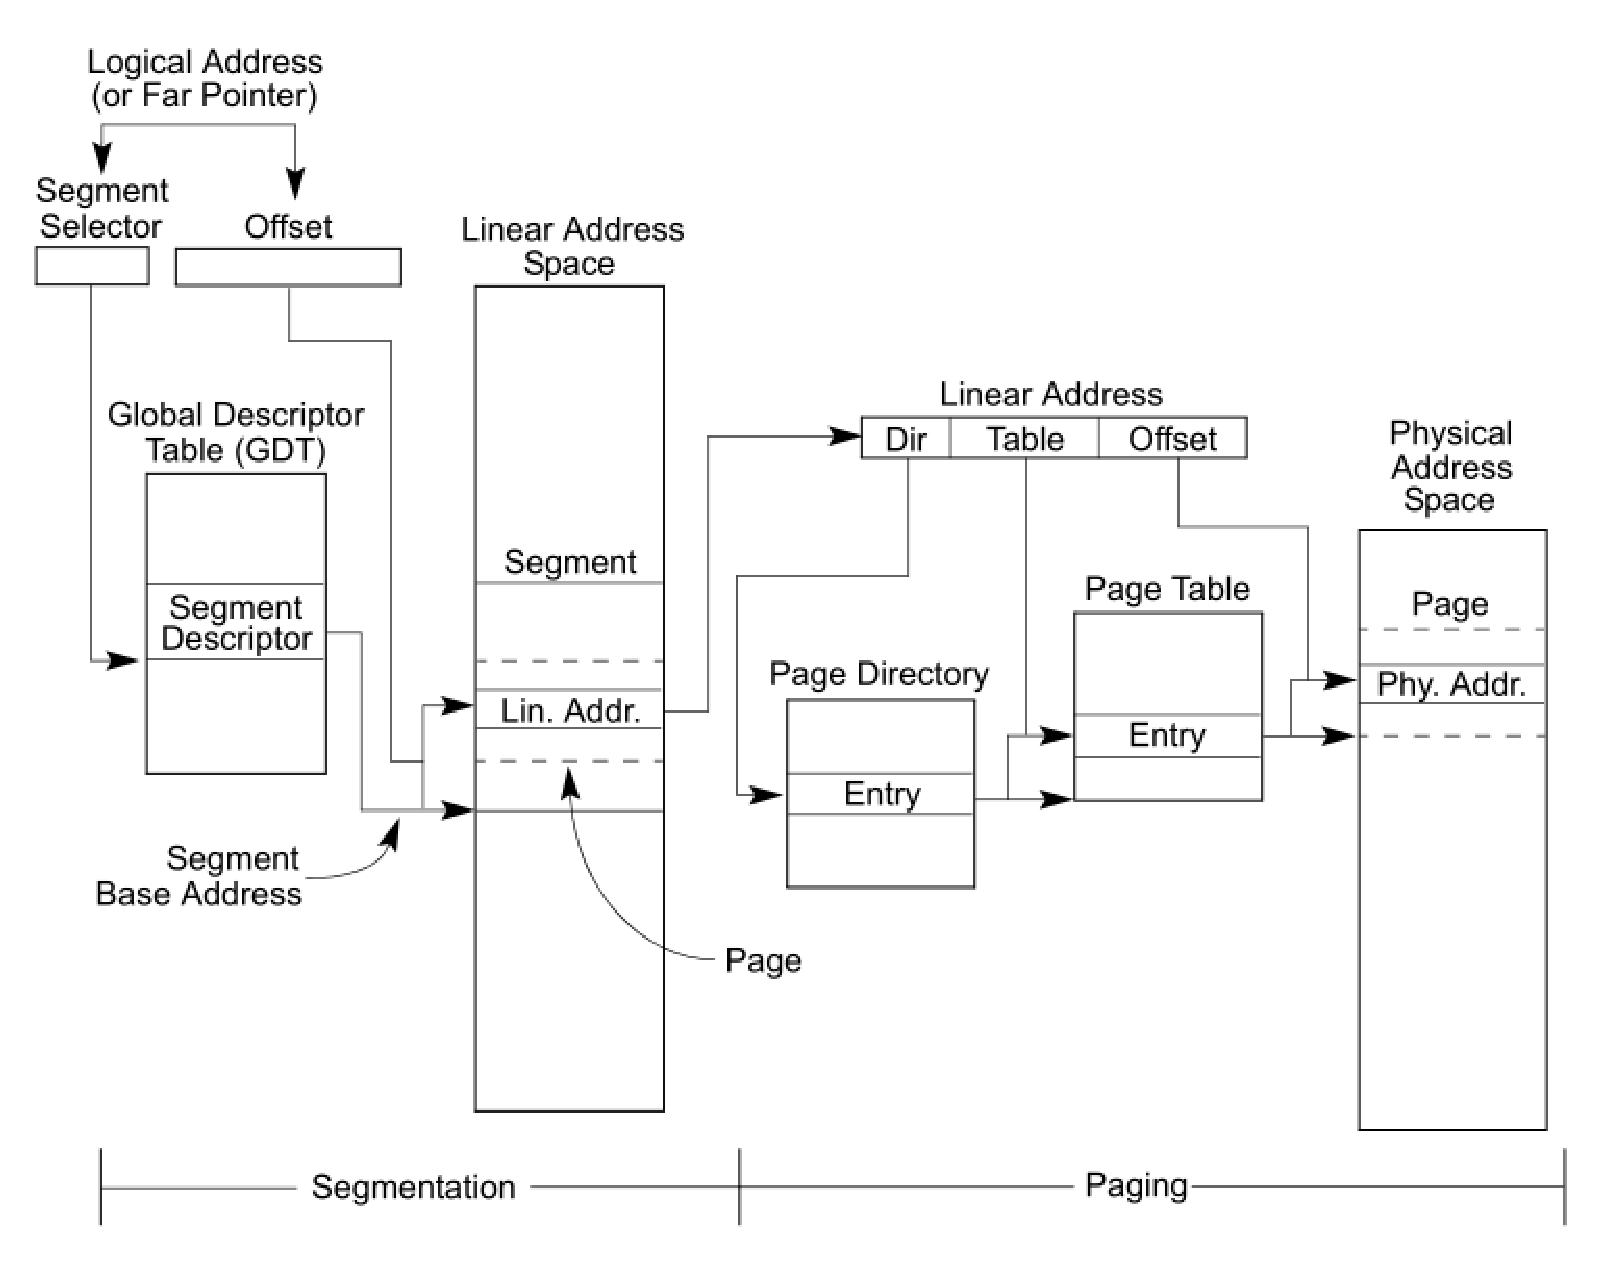
\includegraphics[height=8cm,
    angle=0]{./images/memory_segment.eps}}
\caption{Segmentations}
\label{fig:memory_segment}
\end{figure}

\begin{figure}[hbt]
  \centerline{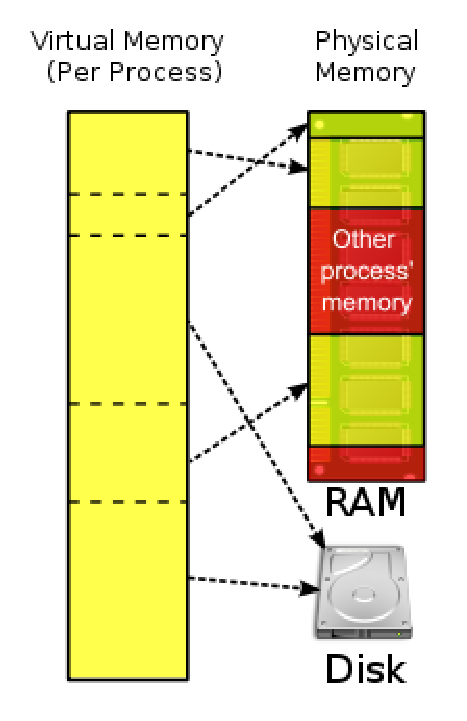
\includegraphics[height=5cm,
    angle=0]{./images/virtual_memory.eps}}
\caption{Virtual memory}
\label{fig:virtual_memory}
\end{figure}

Since 1982, with 80286 CPU, to support multi-tasking, as well as multi-user,
another layer of memory management is added to the kernel of the operating
system. In multi-tasking, the O/S enables the user to switch from one program
to another without exit the current program. As the data of the two programs
are loaded into the memory at the same time, there must be a mechanism to making
sure they are not messing up the data from each other. This is called a {\bf
virtual memory} with a number of modes.

The virtual memory is divided into two parts: user-mode space, and
kernel space, as shown in Fig.~\ref{fig:virtual_address}. They are
normally in the ratio 2G/2G in Windows and 1G/3G in Linux, as shown in
Fig.~\ref{fig:kernel_user}.  The kernel spaces for all processes map
to the same physical kernel space; while the user-mode space from two
different processes never map to the same physical memory location. 
This to ensure the integrity of the O/S, and to protect the O/S from being
attacked by the malicious programs (e.g. virus).

\begin{figure}[hbt]
  \centerline{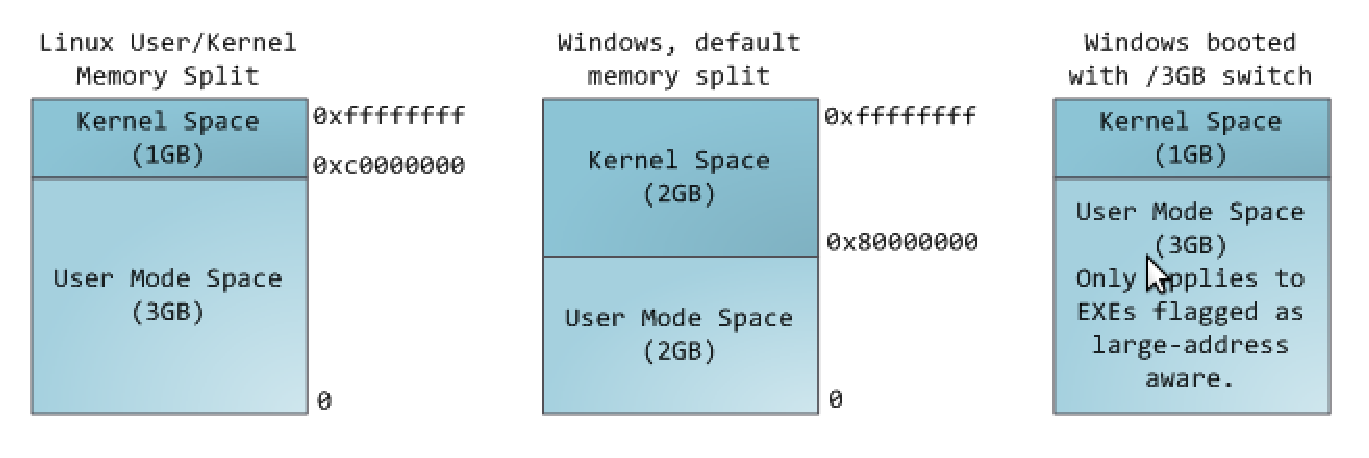
\includegraphics[height=4cm,
    angle=0]{./images/kernel_user_memory.eps}}
\caption{Kernel and User-mode memory space}
\label{fig:kernel_user}
\end{figure}

The {\bf protected mode} was developed to avoid the conflict of memory being
used by one program to another. This virtual memory space are organized into
smaller protected address space called {\it segments}, with code and data are
put into seperates segments (register DS=data segment, and register CS=code
segment). One program cann't access code-segment or data-segment of another
program. A logical address is formed by \verb!segment:offset! pair,
Fig.\ref{fig:memory_segment}. In the basic/protected {\bf flat-model}, only two
segments are created: code segment and data segment being used for all running
programs. In the {\bf multi-segment model}, there are other segments: stack
segment, and more than one data segments.

\begin{enumerate}
  \item in 32-bit addressing: a 16-bit segment registers was introduced that point to the
segment being used by one program, and 32-bit offset selector
\item in 16-bit addressing: a 16-bit segment registers was introduced that point to the
segment being used by one program, and 16-bit offset selector
\end{enumerate} 
The kernel of the O/S will take cares of mapping the logical address to the
physical memory address. 

It's important to know that even though in theory each process has 4GB of
virtual memory, the total memory of all loaded processes, must be less than the
amount of RAM installed + pagefile size (i.e. the amount of hard drive space
being used as RAM). 


\begin{mdframed}
If using 32-bit to address a memory position in the virtual address space, the
maximum linear address space is $2^{32}-1$ (in 32-bit) and $2^{16}-1$ (in
16-bit) which is about 4GB in 32-bit. Since P6 family CPUs, IA-32 architecture
supports $2^{36}-1$=64GB of memory.  
\end{mdframed} 

\section{Pagefile (Windows) vs. Swap space (Linux)}
\label{sec:pagefile}

To allow a program running that uses an amount of memory larger than those
availabel on RAM, Windows O/S  use a fraction of harddisk as
virtual RAM (pagefile). The technique is called {\bf paging} (which can be used with
any segment models).
Paging supports a virtual memory enironment. Here, the processor operates in protected mode; and the
operating system provides virtual management system, e.g. {\bf PAE paging
mechanism}. Example: in 16-bit system, programs run on their own
virtual memory space of 24-bit address line. Then, each program has 16MB virtual
memory space. The OS will manage the mapping this contiguous virtual memory to,
not necessary contiguous, physical main memory and hard drive space, as shown in
Fig.~\ref{fig:virtual_memory}. This make the programming easier as it hide the
fragmentation of data on physical memory.  

In paging, each segment is divided into pages (typically of size 4KByte), which
can be mapped to either physical RAM or harddisk. The operating maintains a
single page-directory and a set of page-tables to keep tracks of pages. A
logical address requires a page-index, and page-offset and map them to physical
address. If the page being access is not in the RAM (as it can be in the
harddisk), a {\it page-fault error} occurs, and the operating system read the
page from harddisk to RAM before continue execution of the program. 




% OS, if all processes are put on the same physical space, how can we
% divide the space to each process. It's not easy as some process is
% large, some is smaller. In addition, one process may access to the
% memory location of another one. To avoid all of these problems, the OS
% create an intermediate layer, by allow each process to have its own
% memory space, known as {\bf virtual memory space}. And the OS will
% manage the loading of codes to virtual memory, as well as mapping it
% to the real physical memory location, as shown in
% Fig. \ref{fig:virtual_address}, when it issues the instruction to CPU.

\begin{figure}[hbt]
  \centerline{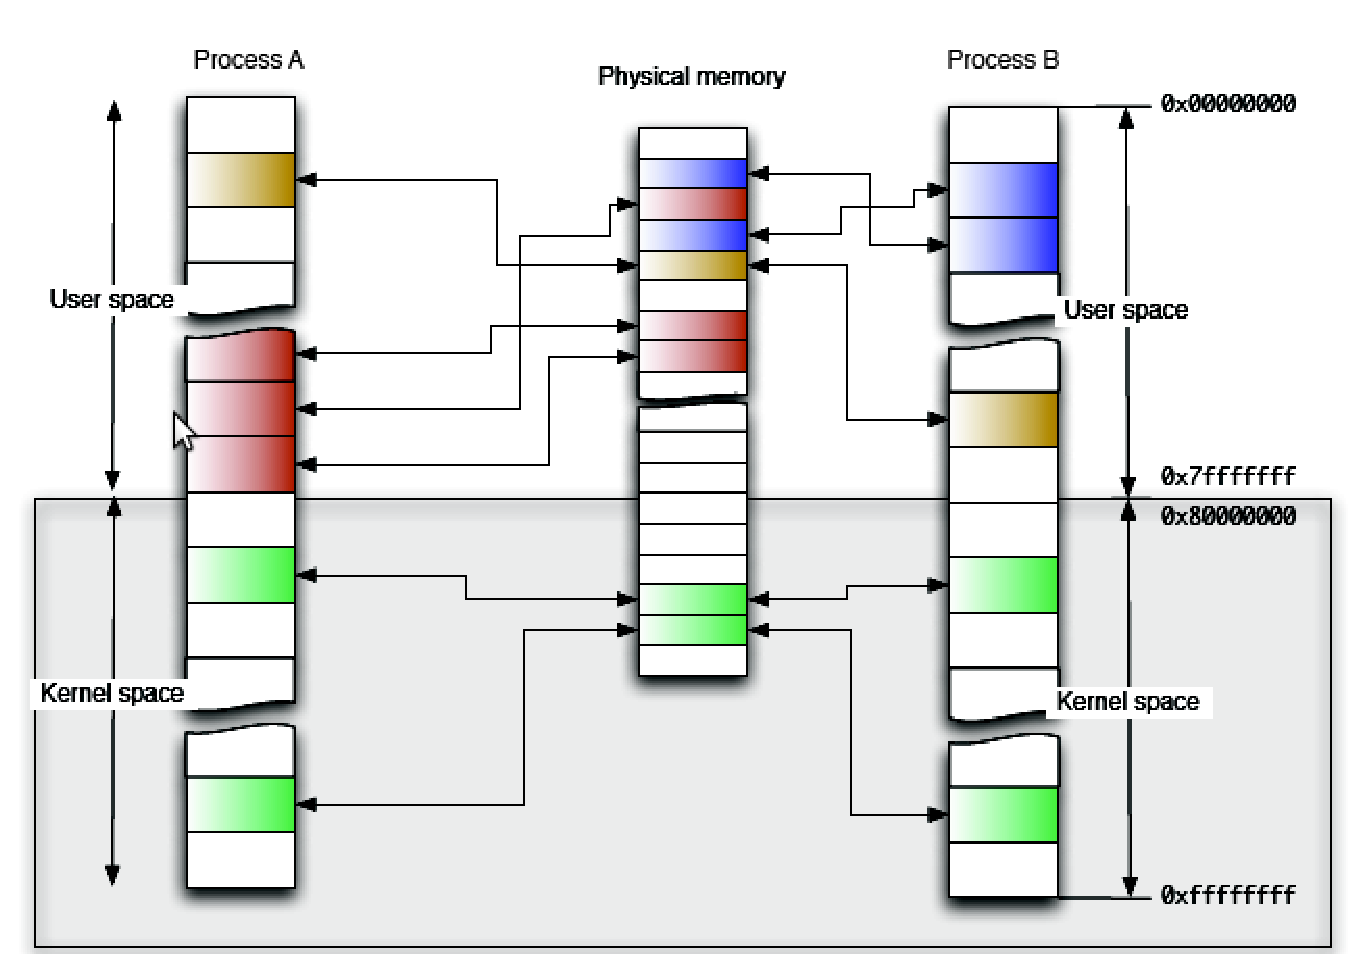
\includegraphics[height=5cm,
    angle=0]{./images/virtual_address.eps}}
\caption{Virtual address}
\label{fig:virtual_address}
\end{figure}

Using virtual memory design, almost all implementation divide the
virtual memory space into blocks of contiguous virtual memory space,
known as {\bf pages}. Pages are homogeneous blocks of 4KB, in most
32-bit systems. Systems with large virtual memory space or large RAM,
generally use larger page size.  They are mapped to physical address
by {\bf page tables} which are maintained by the OS.  With 4GB of
memory, we need 1 Mega (1024x1024) 4KB pages. The CPU use a two-level
structure to map a page to a physical memory location. Consider it as
a 1024x1024 matrix, with the first dimension is Page Directory and the
second dimension is known as the Page
Table\footnote{\url{http://www.intellectualheaven.com/Articles/WinMM.pdf}}.
So, we have 1024 Page Directory, each Page Directory has 1024 Page
Tables, each Page Table has 1024 entries, each of which points to the
initial address of a 4KB page in physical memory, as shown in
Fig.~\ref{fig:paging}.

\begin{figure}[hbt]
  \centerline{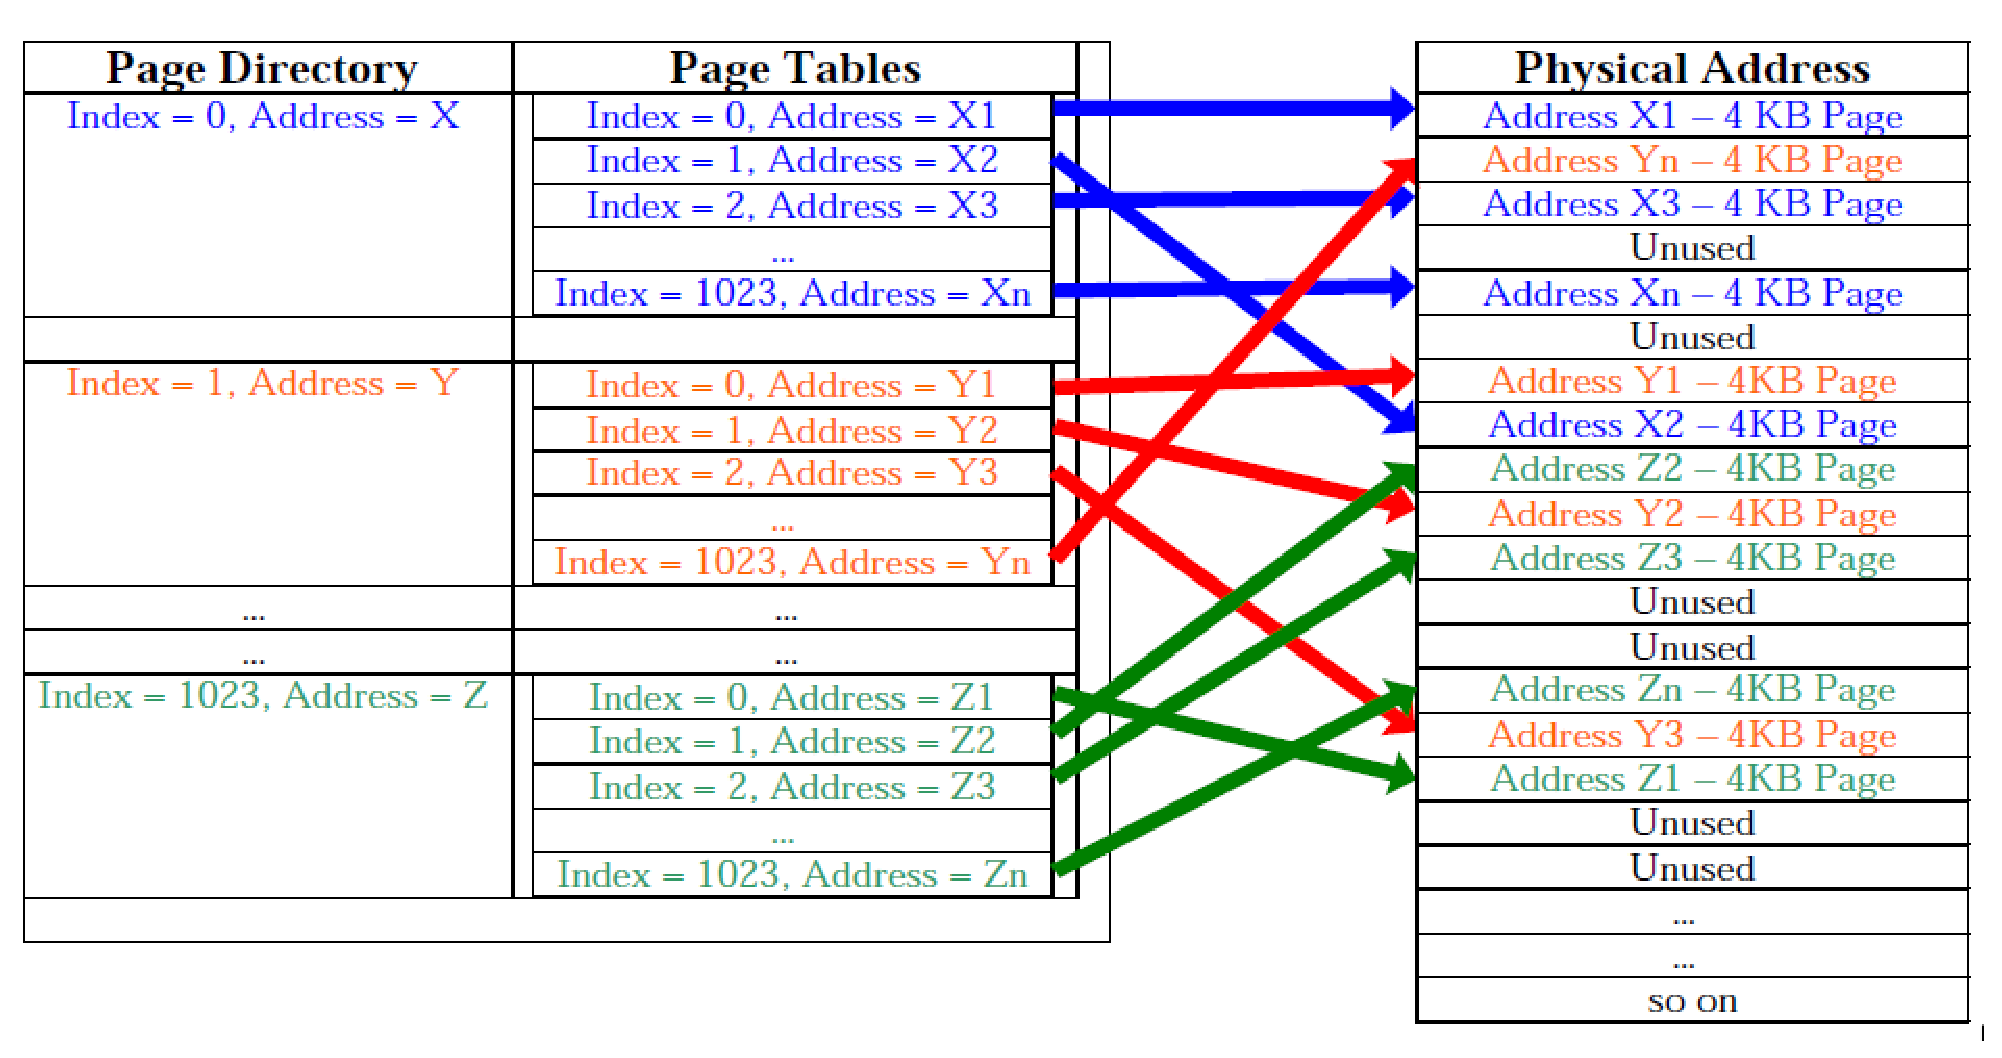
\includegraphics[height=5cm,
    angle=0]{./images/paging.eps}}
\caption{Paging}
\label{fig:paging}
\end{figure}

The total amount of the memory to store Page Directory + Page Table is
4MB = 1024x1024x4. In Windows, each process has its own PD and PT;
thus at least it use 4MB of RAM when it is loaded. The starting
address where the whole PD and PT is stored in RAM is known as
{\bf Page Directory Base} address which is stored in the special CPU
register CR3 (on x86). So, when context switching occur, i.e. CPU
serve a different process, the value of CR3 is changed to the value of
the address of the PDB of the new process, as shown in
Fig.~\ref{fig:paging_register}.
\begin{figure}[hbt]
  \centerline{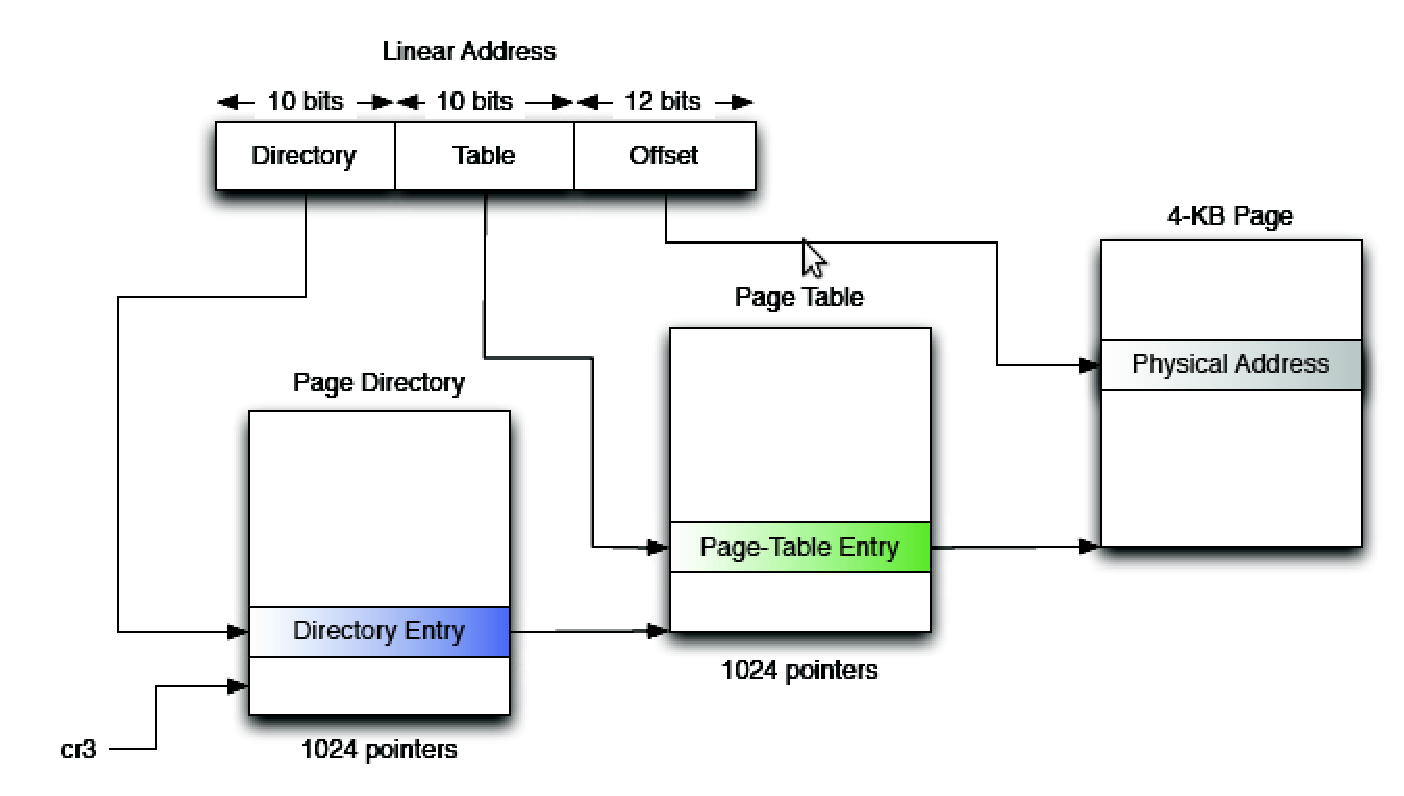
\includegraphics[height=5cm,
    angle=0]{./images/paging_register.eps}}
\caption{Paging and register to address Page Directory, Page Table}
\label{fig:paging_register}
\end{figure}
CR3 is a 32-bit register with the highest 10 bits keep the index of
Page Directory Entry (PDE), the next 10bits keep the index of the Page
Table Entry (PTE), and the last 12 bits to address the individual
bytes in the page (which can address any byte within the 4KB
limit). To avoid user change Page table information, the total 4MB
resides in the kernel logical space, with logical address 0xC000000000
to store the Page Tables and address 0xC0300000 to store page
directory. \textcolor{red}{For 64-bit system, read
  Sec.~\ref{sec:64-bit-systems}.}


{\bf NOTE}: Some virtual pages do not map to any actual physical
memory address, because not all virtual pages are necessarily being
used at any given time; these unused virtual pages are called
invalid. If a program ever tries to access an invalid page, the CPU
traps to the operating system, causing a Segmentation Fault or Access
Violation.

Other systems, rather than use pages, implement a different technique,
known as {\bf segmentation} of variable-length segments. Some systems
combine the two designs, i.e. virtual space is divided into segments,
each segment is divided into pages.

When a program access the unexpected memory, the error
{\it segmentation fault} or {\it general protection fault} occurs,
e.g. de-references a NULL pointer.  However, when running multiple
programs, the memory required is often exceed the RAM installed,
Windows developed create a so-called {\bf pagefile} that use an amount
of physical hard drive spaces to stored the data as RAM. Of course,
accessing data in page memory is slower than in RAM. So, when there is
not enough page in RAM, it save the data to pagefile. We call this
{\bf page eviction}. When these pages are accessed again, the OS
restore theme back to the physical RAM, possibly evicting other
inactive pages to the pagefile. If the process continues to access
pages swap to the disk, then the system will spend most of its time
moving data around from RAM to disk; this will slow down the
performance and is called {\bf thrashing}, i.e. the system does lots
of things but make no useful progress. 


In Linux, instead of using pagfile, it reserved a separate partition,
known as {\bf swap space}, which is normally about 2x of RAM
installed.

References:
\begin{enumerate}
\item
  \url{http://www.cs.miami.edu/~burt/learning/Csc521.071/notes/tovm.html}
\item
  \url{http://duartes.org/gustavo/blog/post/anatomy-of-a-program-in-memory}
\item \url{http://duartes.org/gustavo/blog/post/cpu-rings-privilege-and-protection}
\end{enumerate}

% \section{CPU interact with data in memory (registers, cache, RAM, harddisk)}
% 
% The CPU is the central processing unit that can performs different kinds of
% operations, each one needs to use data to perform its tasks. The data can
% be in one of the different memory spaces (registers, cache, RAM or harddisk). 



\section{Thread Local Storage (TLS)}
\label{sec:TLS}

As threads in the same process share the same memory space, it is sometimes
undesirable. Sometimes it is desirable that two threads referring to the same
static or global variable are actually referring to different memory locations,
thereby making the variable thread-local.
\footnote{\url{http://en.wikipedia.org/wiki/Thread-local_storage}}

A TLS table is 64 slots of 32-bit values, which holds pointers to dynamically
allocated memory that belongs to the thread.


\subsection{C++}

\subsection{C\#}

In C\#, static fields can be marked as thread-local with \verb![ThreadStatic]!
attribute
\begin{verbatim}
class FooBar {
   [ThreadStatic] static int foo;
}
\end{verbatim}

Since .NET 4.0, it has
\begin{verbatim}
 private static System.Threading.ThreadLocal<int> foo;
\end{verbatim}
\url{http://msdn.microsoft.com/en-us/library/dd642243.aspx}


\section{Memory in Win32}
\label{sec:memory-Win32}

Win32 functions allocate memory and put them on {\bf native heap}. There is no
memory manager for this heap; so it is the task of the programmer to free the
memory once it is no longer being used.

Fig.\ref{fig:memory-management-Win32} provides details of how memory objects are
allocated. Depending on the location of the data, Win32 provides 3 groups of
APIs: memory-mapped file functions, heap memory functions, and virtual memory
functions.

\begin{figure}[hbt]
  \centerline{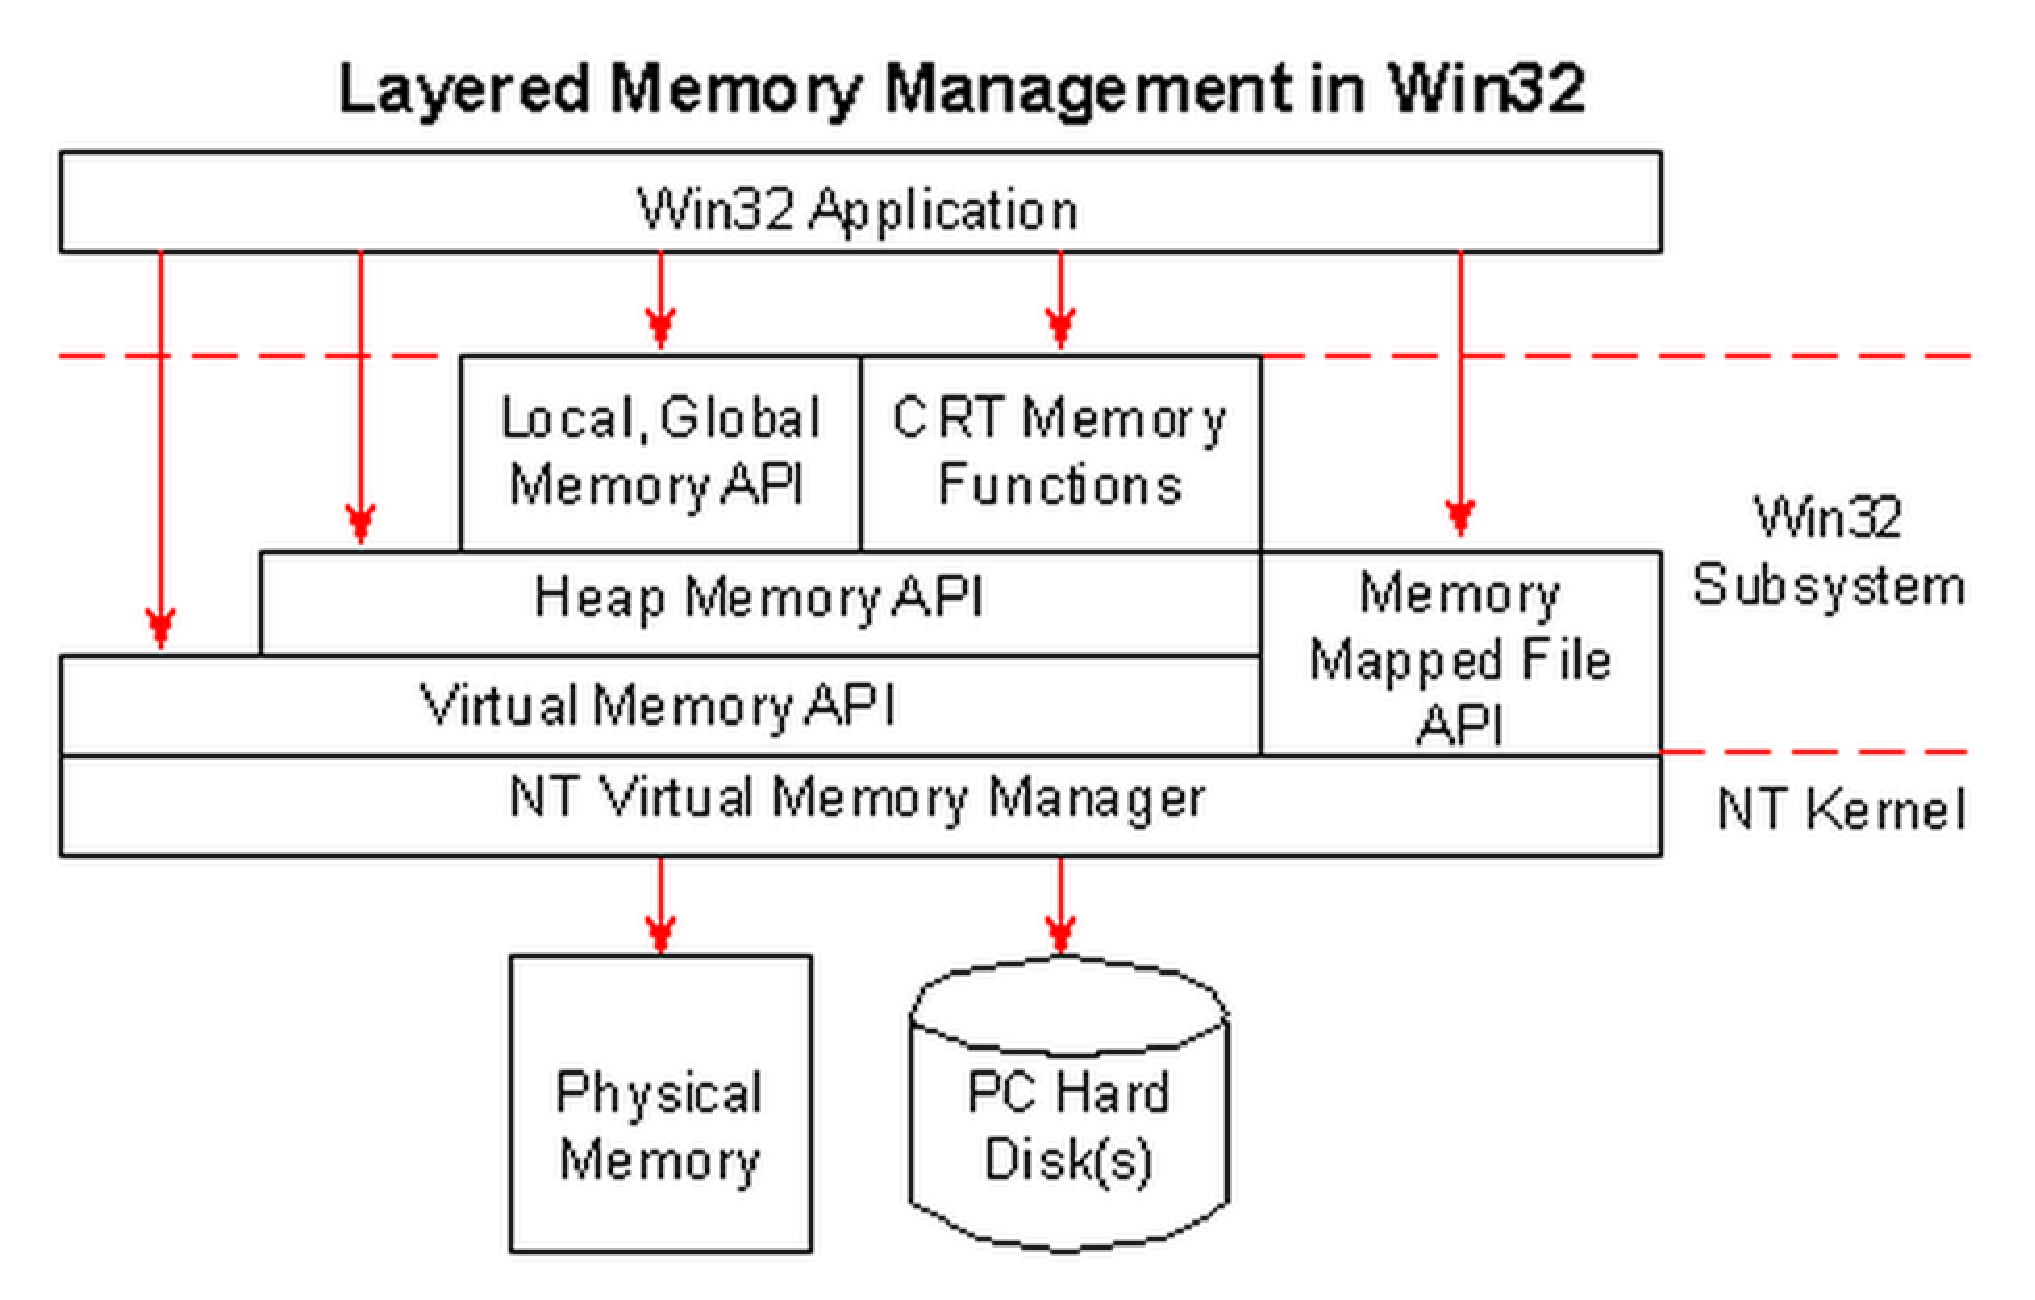
\includegraphics[height=5cm,
    angle=0]{./images/memory-management-win32.eps}}
  \caption{Layers of Memory Management in Win32}
\label{fig:memory-management-Win32}
\end{figure}

\url{http://msdn.microsoft.com/en-us/library/ms810603.aspx}

Generally spoken, Windows offers applications three ways of allocating memory:
{\bf virtual memory}, {\bf shared memory} and {\bf heaps}. The first one is the
primary means by which SQL Server allocates memory when that's needed. The
virtual memory functionality in the Windows OS can be summarized by explaining
the some key functions in the Win32 API to work with this mechanism. Check the
APIs from Platform SDK of Windows XP and Windows Server 2003.

\subsection{Virtual Memory}
\label{sec:virtual-mem-alloc-Win32}

\begin{enumerate}
  \item VirtualAlloc/VirtualFree
  
  \item VirtualLock and VirtualUnlock: to lock the virtual memory in the
  physical memory
  
  \item VirtualProtect: change the protection attributes of a virtual memory
  page; examples of these attributes are 
  \begin{verbatim}
  PAGE_EXECUTE, 
  PAGE_EXECUTE_READ,
  PAGE_EXECUTE_READ_WRITE
  \end{verbatim}
  , etc including support for copy-on-write mechanisms and so on
  
  \item VirtualQuery: obtain information about the virtual memory on the system 
\end{enumerate}

\subsection{Heap memory}

A heap is controlled by a thing called a heap manager and consists of a region
in memory divided in pages of reserved space. The heap manager can be called to
get a piece of memory to work with. Typically heaps are used when objects or
structures with similar sized need to be allocated in memory. An example of the
usage of a heap is the {\bf new} operator in C++ or the {\bf malloc} function in
C.
\begin{enumerate}
  \item HeapCreate and HeapDestroy : create/destroy the so-called private heap
  \item HeapAlloc: like C's malloc()
  \item HeapFree: like C's free()
\end{enumerate}

\subsection{Shared memory}

The idea of shared memory is to allocate a memory region and to allow shared
access to it for multiple processes, so it can be used for inter process data
exchange. 

SQL Server uses shared memory as a fast way to communicate with client
applications {\it on the same machine}, bypassing protocols such as TCP/IP (and
therefore the whole network OSI stack) or named pipes, through the Net-Library
related functionality  

\begin{enumerate}
  \item CreateFileMapping: create a {\it section object} to be used with either
  shared memory or a memory-mapped file
  
  \item MapViewOfFile: creates a mapped view for a file in the physical memory
  
  \item FlushViewOfFile: write the modified pages in the mapped view to disk
\end{enumerate}

\subsection{File mapping}
\label{sec:FileMapping-Win32}

File mapping is the association of a file's contents with a portion of the
virtual address space of a process. The system creates a file mapping object
(also known as a section object) to maintain this association. A file view is
the portion of virtual address space that a process uses to access the file's
contents. File mapping allows the process to use both random input and output
(I/O) and sequential I/O. It also allows the process to work efficiently with a
large data file, such as a database, without having to map the whole file into
memory. Multiple processes can also use memory-mapped files to share data.    

\begin{Verbatim}
//C++
LPVOID WINAPI MapViewOfFile(
  _In_  HANDLE hFileMappingObject,
  _In_  DWORD dwDesiredAccess,
  _In_  DWORD dwFileOffsetHigh,
  _In_  DWORD dwFileOffsetLow,
  _In_  SIZE_T dwNumberOfBytesToMap
);

UnmapViewOfFile
\end{Verbatim}
To specify a suggested base address for the view, use the MapViewOfFileEx
function. However, this practice is not recommended.

The file on disk can be any file that you want to map into memory, or it can be
   the system page file. A process can create multiple views for a file mapping
   object. When multiple processes use the same file mapping object to create
   views for a local file, the data is coherent. That is, the views contain
   identical copies of the file on disk, Fig.\ref{fig:FileMapping}. The file
   cannot reside on a remote computer if you want to share memory between multiple processes.  
   
\begin{figure}[hbt]
  \centerline{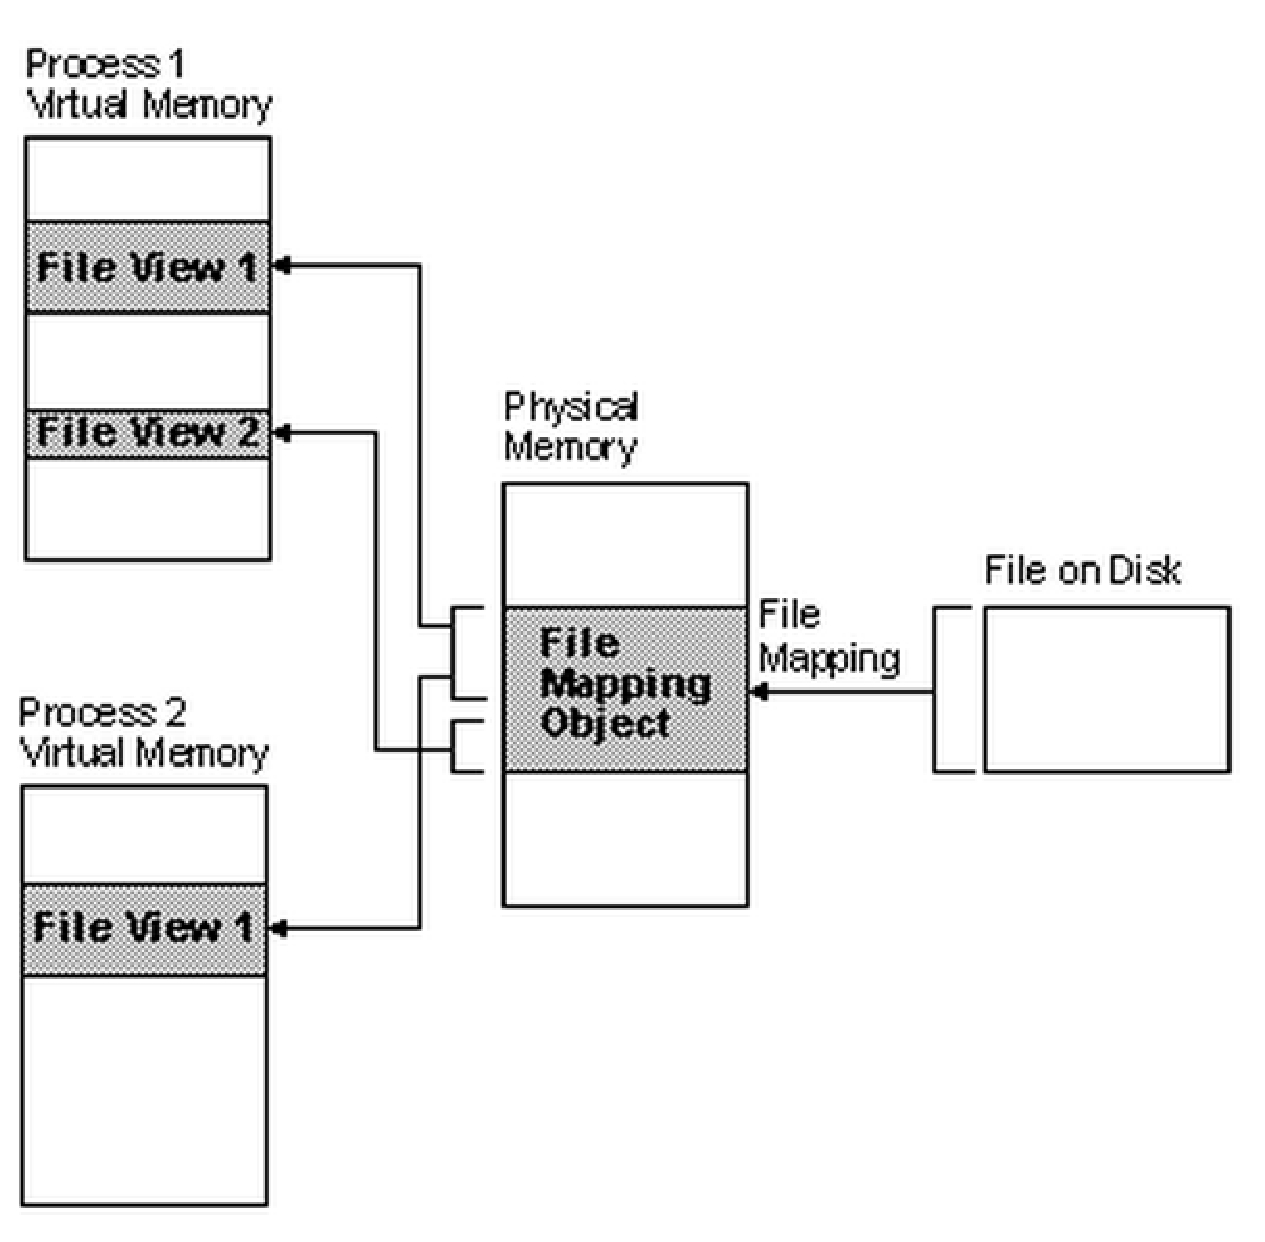
\includegraphics[height=5cm,
    angle=0]{./images/FileMapping.eps}}
  \caption{File Mapping}
\label{fig:FileMapping}
\end{figure}

The equivalent call in Unix is  mmap(2) Unix system call.   

\url{http://msdn.microsoft.com/en-us/library/windows/desktop/aa366556(v=vs.85).aspx}

\import*{../Fortran_manual/}{X86_X86-64.tex}
\import*{../Reverse_Engineering/}{Library.tex}
%\import*{../Fortran_manual/}{Programming_Concepts.tex}
\chapter{Locale - Internationalization - Globalization}
\label{chap:locale}

Locale refers to the way the application behaves acoording to the user's
language environment. This include character encoding, formatting of
dates/times, currency and large numbers.

Support for international locale started since C89 (Sect.\ref{sec:C89_locale}).
A (character) language environment defines
\begin{enumerate}
  \item native language of the country-specific
  \item character set and coded character set : how to map a character of a
  character set into a code point in a set of code points. A code point is a
  hexadecimal value (binary value if stored in computer). 

  \item collating and ordering: define the relative orders of characters (used
  for sorting)
  
  \item character classification: define the type of characters in which groups
  (alphabetic, numeric)
  
  \item character case conversion: mapping between lower case and upper case
  
  \item data, time format: names of the weekdays, order of months, etc.
  \item format of numbers and monetary quantities: numeric grouping,
  decimal-point character, and monetary symbols.
  
  \item format of affirmative and negative system responses: 
\end{enumerate}
A \verb!locale! tells us how the language-specific data (given above)
is processed, data I/O (printed and displayed). 

Before you can compile your program, the compile must be able to read the source
code. So, it's important to tell the compiler which encoding
scheme of the source file (Sect.\ref{sec:locale_source-files})

% What it tells is It mainly deals with character and string processing.

You can set the locale in the code so that it knows how to interpret data based
on that locale. A locale define the code sets, date and time formatting conventions,
monetary conventions, decimal formatting convention, etc. Each can be set by
modifying a given environment variable, which can be
queried using \verb!locale! command.
\begin{verbatim}
LANG=en_US.UTF-8
LANGUAGE=
LC_CTYPE="en_US.UTF-8"
LC_NUMERIC="en_US.UTF-8"
LC_TIME="en_US.UTF-8"
LC_COLLATE="en_US.UTF-8"
LC_MONETARY="en_US.UTF-8"
LC_MESSAGES="en_US.UTF-8"
LC_PAPER="en_US.UTF-8"
LC_NAME="en_US.UTF-8"
LC_ADDRESS="en_US.UTF-8"
LC_TELEPHONE="en_US.UTF-8"
LC_MEASUREMENT="en_US.UTF-8"
LC_IDENTIFICATION="en_US.UTF-8"
LC_ALL=
\end{verbatim}
At the machine level, the locale name can be set in the \verb!LANG! environment
variable. If set inside the program, it overwrite the setting in the environment
variable. 

C or POSIX locale is the set of locale setting that is required for all
POSIX-compliant systems/softwares. Single UNIX Specification (SUS) version 3
defined \verb!C locale! (Sect.\ref{sec:LSB_C-lang}).  
\url{http://www-01.ibm.com/support/knowledgecenter/ssw_aix_53/com.ibm.aix.nls/doc/nlsgdrf/locale.htm}
``C'' and ``POSIS'' are the same. 
On GNU systems, only \verb!LC_ALL=C! or \verb!LC_ALL=POSIX! or
\verb!LC_MESSAGE=C|POSIX! override \verb!$LANGUAGE!
setting.\footnote{\url{http://unix.stackexchange.com/questions/87745/what-does-lc-all-c-do}} 

A C program (automatically) inherits the locale information from the environment
variables when it starts up. However, it doesn't control how the locale used by
the library function. Thus, to ensure all the functions (including in the
library) use the locale specified by the environment, we run \verb!locale()!
function with \verb!LC_ALL! as the first argument and an empty string in the
second argument.

\begin{verbatim}
#include <locale.h>

int main()
{
  char* locale;
  locale = setlocale(LC_ALL, "C");  /* set using C-locale */
  locale = setlocale(LC_ALL, "");  /* set based on environment variables */
  
  return 0;
}
\end{verbatim}
\url{http://www.gnu.org/software/libc/manual/html_node/Setting-the-Locale.html}


See how different locales' behavior?
\begin{verbatim}
$ LC_TIME=fr_FR.UTF-8 date
jeudi 22 aot 2013, 10:41:30 (UTC+0100)

$ LC_MONETARY=fr_FR.UTF-8 locale currency_symbol


$ LC_ALL=es_ES man
Que pgina de manual desea?

$ LC_ALL=C man
What manual page do you want?

$ LC_ALL=en_US sort <<< $'a\nb\nA\nB'
a
A
b
B

$ LC_ALL=C sort <<< $'a\nb\nA\nB'
A
B
a
b
\end{verbatim}


Example: converting ASCII to UPPERCASE
\begin{verbatim}
auto loc = std::locale("");

char s[] = "hello";
for (char &c : s) {
  c = toupper(c, loc);
}
\end{verbatim}

Example: To be internationalize, we use \verb!wchar_t! instead.
\begin{verbatim}
auto loc = std::locale("");

wchar_t s[] = L"hello";
for (wchar_t &c : s) {
  c = toupper(c, loc);
}
\end{verbatim}

\chapter{Data types}

When you use data, it's important to know about data alignment
(Sect.\ref{sec:data-alignm-gran} and Sect.\ref{sec:memory_alignment}),
especially in struct or class. It's important to know about (1) declaration
specifiers and (2) declarator-id.
\begin{verbatim}
static unsigned long int *x[N];
\______________________/  \___/
     /                     \
    /                       \
 declaration specifiers   declarator-id   
\end{verbatim}

\begin{itemize}
  \item  A {\bf declarator-id} (id) is the name being declared, here is \verb!x!, possibly
surrounded by {\it operators} such as *, [], (), and (in the case of C++)
\verb!&!.  A declarator may not contain any operator at all, e.g.
\begin{verbatim}
int x;
\end{verbatim}

   \item In a {\bf declaration specifiers}, there are two groups: (1) type specifiers which
contribute to the type of the declarator-id, (2) non-type information that
applies directly to the declarator-id. Here, \verb!unsigned long int! is the
type-specifier, and \verb!static! is the non-type information that tell \verb!x!
has statically allocated storage (Sect.\ref{sec:static_C}).
\end{itemize}


\section{Introduction}

\subsection{aggregate (a special type of class): C++98/03}
\label{sec:aggregate-class}
\label{sec:aggregate-class-C++98-C++03}

Definition in C++98/03 for \textcolor{red}{aggregate}: An aggregate is an array
or a class (clause 9) with no user-declared constructors (12.1), no private or
protected non-static data members (clause 11), no base classes (clause 10), and
no virtual functions (10.3).

First of all, any array is an aggregate. An array is an aggregate even if it is
an array of non-aggregate class type.

In C++, the term \verb!class! refers to all classes, structs, and unions A class
(or struct, or union) is an aggregate if and only if it satisfies the criteria
from the above definitions.
\begin{enumerate}
  \item This does not mean an aggregate class cannot have constructors, in
  fact it can have a default constructor and/or a copy constructor as long as
  they are implicitly declared by the compiler, and not explicitly by the user  
  
  \item No private or protected non-static data members. 
  
  You can have as many private and protected member functions (but not
  constructors) as you like and not violate the rules for aggregate classes
  
  You can have as many private or protected static data members and member
  functions as you like and not violate the rules for aggregate classes
  
  \item An aggregate class CAN have a user-declared/user-defined copy-assignment
  operator and/or destructor
  
  \item 
\end{enumerate}

Below are example of VIOLATION, i.e. NOT an aggregate.
\begin{lstlisting}
class NotAggregate1
{// No virtual function
  virtual void f() {} //remember? no virtual functions
};

class NotAggregate2
{// data MUST be public 
  int x; //x is private by default and non-static 
};

class NotAggregate3
{// No user-defined constructor
public:
  NotAggregate3(int) {} //oops, user-defined constructor
};

class Aggregate1
{
public:
  NotAggregate1 member1;   //ok, public member
  Aggregate1& operator=(Aggregate1 const & rhs) {/* */} //ok, copy-assignment  
private:
  void f() {} // ok, just a private function
};
\end{lstlisting}


\subsection{aggregate in C++11}
\label{sec:aggregate-class-C++11}


The standard definition of an aggregate has changed slightly, but it's still
pretty much the same: 
{\it An aggregate is an array or a class (Clause 9) with no {\bf user-provided
constructors} (12.1), {\bf no brace-or-equal-initializers for non-static data
members (9.2)}, no private or protected non-static data members (Clause 11), no
base classes (Clause 10), and no virtual functions (10.3).  
}  (the bold text is the new part).
\begin{enumerate}
  \item  Previously, an aggregate could have no user-declared constructors, but
  now it can't have user-provided constructors. Is there a difference? Yes,
  there is, because now you can declare constructors and default them:  
  
\begin{verbatim}
struct Aggregate {
    Aggregate() = default; // though declared by user, it asks the compiler to
                          // generate the default implementation
};
\end{verbatim}  

With C++11, this is still an aggregate because a constructor (or any special
member function) that is defaulted on the first declaration is not
user-provided.
  
  \item  with this new standard, we can initialize members directly in the class
  like this:
  
\begin{verbatim}
struct NotAggregate {
    int x = 5; // valid in C++11
    std::vector<int> s{1,2,3}; // also valid
};
\end{verbatim}
Using this feature makes the class no longer an aggregate because it's basically
equivalent to providing your own default constructor.

\end{enumerate}

 

\subsection{Why we use aggregate data type}
\label{sec:aggregate-class-wht-we-use-it}

Unlike non-aggregate classes, can be initialized with curly braces
\verb!{}!. This initialization syntax is commonly known for arrays,

\begin{verbatim}
// notice the different name 'm' and 'n'
// which mean we can initialize an array of size 'n'
//   with less values

Type array_name[n] = {a1, a2, ..., am};
\end{verbatim}
It means that
\begin{itemize}
  \item if 'm < n': he first m elements of the array are initialized with a1,
  a2, ..., am and the other $(n - m)$ elements are, if possible,
  value-initialized (Sect.\ref{sec:value-initialized}). 
  
  \item if 'm = n': ith element of the array is initialized with ai
  
  \item if 'm > n':  compiler will issue an error
\end{itemize}

Example:
\begin{lstlisting}
class A
{
public:
  A(int) {} //no default constructor
};
class B
{
public:
  B() {} //default constructor available
};


int main()
{
  A a1[3] = {A(2), A(1), A(14)}; //OK n == m
  A a2[3] = {A(2)}; //ERROR A has no default constructor. Unable to value-initialize a2[1] and a2[2]
  B b1[3] = {B()}; //OK b1[1] and b1[2] are value initialized, in this case with the default-ctor
  int Array1[1000] = {0}; //All elements are initialized with 0;
  int Array2[1000] = {1}; //Attention: only the first element is 1, the rest are 0;
  bool Array3[1000] = {}; //the braces can be empty too. All elements initialized with false
  int Array4[1000]; //no initializer. This is different from an empty {} initializer in that
  //the elements in this case are not value-initialized, but have indeterminate values 
  //(unless, of course, Array4 is a global array)
  int array[2] = {1, 2, 3, 4}; //ERROR, too many initializers
}
\end{lstlisting}

\subsection{Initialize data}

In C++1998 there are 2 types of initialization: zero and default.
\begin{verbatim}
new A - indeterminate value
new A() - zero-initialize

new B - default construct (B::m is uninitialized)

new B() - default construct (B::m is uninitialized)

new C - default construct (C::m is zero-initialized)

new C() - default construct (C::m is zero-initialized)
\end{verbatim}

In C++2003 a 3rd type of initialization, value initialization was added.
\begin{verbatim}
new A - indeterminate value

new A() - value-initialize A, 
          which is zero-initialization if A is a POD.

new B - default-initializes (leaves B::m uninitialized)

new B() - value-initializes B which zero-initializes all fields since its default ctor is compiler generated as opposed to user-defined.

new C - default-initializes C, which calls the default ctor.

new C() - value-initializes C, which calls the default ctor.
\end{verbatim}

\subsection{zero-initialized}

\subsection{default-initialized}

\subsection{value-initialized (since C++2003)}
\label{sec:value-initialized}	


The definition below is imprecise and a bit incorrect but it should give you the
basic idea.
\begin{itemize}
  \item When an object of scalar type (bool, int, char, double, pointers, etc.) is
{\bf value-initialized} it means it is initialized with 0 for that type (false
for bool, 0.0 for double, etc.). When an object of class type with a user-declared
default constructor is value-initialized its default constructor is called.

  \item If the default constructor (of a class) is implicitly defined (i.e. by
  the compiler, NOT by the user) then all nonstatic members are recursively
value-initialized.
\end{itemize}

A reference cannot be value-initialized. Value-initialization for a
non-aggregate class can fail if, for example, the class has no appropriate
default constructor. 




\subsection{POD type (Plain-Old Data type)}
\label{sec:POD-plain-old-datatype}

POD stands for Plain Old Data - that is, a class (whether defined with the
keyword \verb!struct! or the keyword \verb!class!) without constructors,
destructors and \verb!virtual! members functions
(Sect.\ref{sec:virtual_member-function}).

\textcolor{red}{Why POD}: Compiling a POD in C++ gives you the same memory
layout as a struct compiled in C.


POD is all built-in data types (e.g. int, char, float, long, unsigned char,
double, etc.) and all aggregation (Sect.\ref{sec:aggregate-class}) of POD data. 

How to check if something is a POD? Well, there is a struct for that called
\verb!std::is_pod!
\begin{verbatim}
namespace std {
// Could use is_standard_layout && is_trivial instead of the builtin.
template<typename _Tp>
  struct is_pod
  : public integral_constant<bool, __is_pod(_Tp)>
  { };
}
\end{verbatim}

In C++ 98/03, a Plain Old Data Structure in C++ is an aggregate class that
contains only PODS as members, has no user-defined destructor, no user-defined copy
assignment operator, and no nonstatic members of pointer-to-member type.
\url{https://stackoverflow.com/questions/4178175/what-are-aggregates-and-pods-and-how-why-are-they-special/4178176#4178176}

In C++11, 


\subsection{non-POD data types}
\label{sec:non-POD-class}


A POD type is a C++ type that has an equivalent in C, and that uses the same
rules as C uses for initialization, copying, layout, and addressing.


A non-POD class is a class that contains a user-defined constructor, or
destructor, or virtual functions, or derived from a base class, or contains
members that are one of the ones I mentioned.

In other words, if the type is not 'C' compatible, it is non-POD.

\url{http://www.parashift.com/c++-faq-lite/pod-types.html}



\subsection{Name lookup}

C++ classifies names in different ways, i.e. different terminologies. 

\begin{itemize}
  \item identifier : a name consisting of an uninterupted sequence of letters,
  underscotre (\verb!_!) and digits. CONSTRAINTS: it cannot start with a digit,
  and some are reserved as keywords. NOTE: The concept of letters should be
  taken broadly and includes universal character names (UCN)
  
  \item operator-function-id: 
\begin{verbatim}
operator new
operator []
operator &
\end{verbatim}

   \item conversion-function-id: denote a user-defined implicit conversion
   operator
\begin{verbatim}
operator int&
\end{verbatim}

   \item template-id: 
\begin{verbatim}
List<T, int, 0>
\end{verbatim}

   \item unqualified-id: it can be any of the (identifier,
   operator-function-id, conversion-function-id, template-id) or a destructor
   name 
\begin{verbatim}
~Data
~List<T, T, N>
\end{verbatim}

   \item qualified-id: an unqualified-id becomes a qualified-id when it comes
   with namespace or class information, or just the global scope resolution
   operator
\begin{verbatim}
::X			// NOTE: ::X refer to the type
S::x
Array<T>::y
::N::A<T>::z
\end{verbatim}
\end{itemize}

There are two non-standard terms:
\begin{itemize}
  
   \item \verb!qualified name!: a name that undergoes a qualified lookup, in
   which the scope to which the name belongs is explicitly mentioned using a
   scope operator (::) or a member access operator (\verb!->! or \verb!.!).
   
\begin{verbatim}
this->count 	;// qualified name

count 			// unqualified name
\end{verbatim}
   
  
%   \item \verb!unqualified name!:

  \item a {\bf dependent name} : a name that depends in some way to a
  template parameter
\begin{verbatim}
std::vector<T>::iterator      // an dependent name if T is a template parameter

std::vector<int>::iterator      // a nondependent name

ident(x,y,z)      // 'ident' is a dependent name if and only if
                  // any of its argument has a type that depends on 
                  // a template parameter
\end{verbatim}
      
\end{itemize}

% However, there are two major naming concepts:
% \begin{enumerate}
%   \item a {\bf qualified name} : 
% \end{enumerate}

Name lookup attempts to find all names available at the point of usage. 
\begin{enumerate}
  \item  If the
qualified name has the scope is a class, then the base class is also searched,
before any other enclosing scopes, i.e. wrapped by \verb!{ ... }!
\begin{verbatim}
int x;
class B{ int i;};
class D::public B{};
void foo(D* pd) {
  pd->i = 3; // find B::i
  D::x = 1 ; // error, do not find ::x in the enclosing scope
}
\end{verbatim}
  
   \item The unqualified name go through (1) ordinary lookup, i.e. is looked up
   in a successively manner from the inner nost scope to the outer scope via
   enclosing scopes, (2) or sometimes undergoes {\it argument-dependent lookup}
   (ADL or Koenig lookup, extended Koenig lookup - named after Andrew Koenig).
   
\begin{verbatim}
extern int count ;; // (1)

int lookup_(int count) // (2)
{
   if (count < 0) {
       int count = 1;  // (3)
       lookup_(count)  // use 'count' in (3)
   }
   
   return count +  ::count; 
      // the first and unqualified 'count' is from (2)
      // the second and qualified 'count' is from (1)
}
\end{verbatim}
\end{enumerate}

\subsection{Qualified and unqualified types}

In computer programming, a fully qualified name is an unambiguous name that
specifies which object, function or variable the name refer to without regarding
to the context of using it. 
\begin{itemize}
  \item In Unix pathname, the full pathname should start with \verb!/!, e.g.
  /home/user/this/folder/file.txt
  
  \item In URL: wikipedia.com/thisfile
  \item In C++, Tcl, Perl, Ruby: So, the namespace should be explicit, and the two
colons (::) is used to distinguish a fully qualified name from a regular name.

\begin{verbatim}
 // Perl
$package2::scalar
 
  // C++
std::vector  
\end{verbatim}
  
\end{itemize}




A {\bf qualified} name is the one that has some sort of indication of where it
belong, e.g. class specification, namespace specification. 


 A {\bf qualified} data type is a built-in data type that has information
about the storage size, range of values, or precision of the type.  


From C99 standard,
the intrinsic data type are {\it unqualified}
\begin{verbatim}
Any type so far mentioned is an unqualified type. Each unqualified type has
several qualified versions of its type, corresponding to the combinations of
one, two, or   all three of the const, volatile, and restrict qualifiers.

The qualified or unqualified versions of a type are distinct types that belong
to the same type category and have the same representation and alignment
requirements.   
\end{verbatim}

To make a type qualified, we use a type qualifier which was introduced in ANSI
C. NOTE: The qualifier not part of the ANSI C89/90 has two leading underscores,
as the extension, and become normal in C99
\begin{enumerate}
  \item \verb!const!: Sect.\ref{sec:const_C} and Sect.\ref{sec:const_C++}.
  
prohibit writing access, i.e. eliminate potential side-effects across function
calls involving the single object. Notice the difference in {\bf down
qualification} between C and C++. C++ being more type restrictive, will not
allow implicit down qualification. However, C++ allows implicit up
qualification.

  \item \verb!volatile!: Sect.\ref{sec:volatile_C}
  
disable optimization on object's storage, i.e. allowing an object to reside on
the global memory that is accessible by other processes or hardware.
   
  \item \verb!__unaligned! :
  
Typically, the memory address of an allocator-id is the multiple of the size of
the type. This is known as {\it aligned memory}. However, when using packed
structures, unaligned memory can occur. A pointer pointing to non-aligned memory
can cause alignment error. To tell the compiler to generate additional code, we
declare the pointer as \verb!__unaligned!
  
  \item \verb!__restrict! (apply to pointer type only),
  or \verb!restrict! (from C99):  Sect.\ref{sec:pointer_restrict}
  
\end{enumerate}
Using type qualifier, it gives greater control over compiler's optimizations.




\section{Macro values}


The maximum value for a floating-point is represented as
\begin{itemize}
  \item in C: use \verb!FLT_MAX! (defined in \verb!<float.h>!)
  \item in C++: use \verb!FLT_MAX! (defined in \verb!<cfloat>!)
  \item in pure C++: use \verb!std::numeric_limits<float>::max! (defined in
  \verb!<climits>!)
\end{itemize}
NOTE: \verb!MAXFLOAT! is a non-standard macro name.

Many other macros are defined in header files 
\begin{itemize}
  \item  \verb!<climits>! (limits.h):  defines constants with the limits of
  fundamental integral types
  
Example: \verb!LONG_MIN!, \verb!INT_MIN!  
  
  \item \verb!<cfloat>! (float.h): define the limits for fundamental
  floating-point type
  
  \item \verb!<cstdint! (stdint.h): define the  limits for width-specific
  integral types and other typedef types
\end{itemize}
\url{http://www.cplusplus.com/reference/climits/}


\section{Header files}

\subsection{stddef.h (cstddef)}
\label{sec:stddef.h}


The header file \verb!stddef.h! defines certain types.  This file must be
included in all kinds of programs as it defines essential macros: NULL (which
is can also be found in other header files: stdio.h, stdlib.h, string.h,
time.h, wchar.h)

\begin{verbatim}
ptrdiff_t            a signed integer type that represents 
                     the result of pointer subtraction
                      
size_t               unsigned integral type that represents
                     the result of sizeof() operations
                     (found in <stddef.h>, stdlib.h, wchar.h, 
                     stdio.h, string.h) 
                     
max_align_t  [C11/C++11] (type with widest scalar alignment)
nullptr_t    [C11/C++11] (null-pointer type)

wchar_t              wide-character type
                     (found in <stddef.h>, <stdlib.h>, <wchar.h>
                      <cwchar>(C++), 
\end{verbatim}

In C++, their namespace is \verb!std!, e.g. \verb!std::ptrdiff_t!. 
The macros representing the range of values for the above types are defined in
the header file \verb!stdint.h!
\begin{verbatim}
  TYPE        MIN/MAX
ptrdiff_t    PTRDIFF_T_MIN    PTRDIFF_T_MAX
             -65535           +65535

size_t       N/A                SIZE_MAX
                                65535
                                
wchar_t         WCHAR_MIN       WCHAR_MAX

\end{verbatim}


\begin{enumerate}
  \item \verb!ptrdiff_t! : an alias of signed integer type, to represent the
  result of any valid pointer-subtraction operation. This is only used in the
  case of pointers to element of an array.
  
  \item \verb!size_t! : an alias of the unsigned integer type, which is used to
  represent the size of any objects in bytes; i.e. this is the type of the value
  returned by \verb!sizeof()! operator.
  
NOTE: \verb!size_t! is used as the type of the parameters (typically to
represent the length (count in bytes) of a string or a specific buffer) in some
functions from \verb!<cstdlib>! header-file, e.g \verb!bsearch, qsort, calloc!,
\verb!malloc!, \verb!realloc!, \verb!mblen, mbtowc, mbstowc, wcstombs!.

  \item \verb!max_align_t! :  Sect.\ref{sec:memory_alignment}
  
\end{enumerate}

The file \verb!stddef.h! (or cstddef) also defines some macros
\begin{verbatim}
NULL                   (null-pointer)
offsetof(...)          (return the member offset)
\end{verbatim}

\section{Type check}


\subsection{typeof()}
\label{sec:typeof}

In C, GCC provides as an extension, while in C++, we need to use Boost library. 
However, it only gives the type of any expression at compile time.

Then we can use
\begin{lstlisting}
  #define max(a,b) \
       ({ typeof (a) _a = (a); \
           typeof (b) _b = (b); \
         _a > _b ? _a : _b; })
\end{lstlisting}

C++ Boost: use \verb!demangle()!
\begin{lstlisting}
#include <boost/units/detail/utility.hpp>

To_main_msg_evt ev("Failed to initialize cards in " + boost::units::detail::demangle(typeid(*_IO_card.get()).name()) + ".\n", true, this);
\end{lstlisting}
\url{http://stackoverflow.com/questions/1986418/typeid-versus-typeof-in-c}

Since C++11, the standard is \verb!decltype()! (Sect.\ref{sec:decltype}).
Also, for runtime type detection, use \verb!typeid! (Sect.\ref{sec:typeid})

\subsection{name demangle}
\label{sec:name_mangling}

Transforming C++ ABI identifiers (like RTTI symbols) into the original C++
source identifiers is called 'demangling.'

\begin{lstlisting}
// https://gcc.gnu.org/onlinedocs/libstdc++/manual/ext_demangling.html


\end{lstlisting}


\subsection{decltype (C++11)}
\label{sec:decltype}

C++11 introduces \verb!decltype()! as a way to return the type of the argument
which can be an object or a function at {\it compile-time} 

\begin{lstlisting}
vector<int> v;
decltype(v)::value_type i = 0; // int i = 0;

const int&& foo();
const int bar();
int i;
struct A { double x; };
const A* a = new A();
decltype(foo()) x1; // type is const int&&
decltype(bar()) x2; // type is int
decltype(i) x3; // type is int
decltype(a->x) x4; // type is double
decltype((a->x)) x5; // type is const double&
\end{lstlisting} 

\subsection{typeid: <typeinfo> (C++11) - RTTI}
\label{sec:type_info}
\label{sec:typeid}
\label{sec:RTTI}

C++11 provides a feature called RTTI ({\bf Runtime Type Identification}) that
allows the code to detect the type (e.g. class-name) of an object at runtime.
We use header file \verb!<typeinfo>! and the function \verb!typeid()!.

Example: inside the class method
\begin{verbatim}
std::cout << typeinfo(*this).name() ;


// if we already know the class-name
// we can use macro

#define quote(x) #x
std::cout << quote(classA);

\end{verbatim}

Example: on an object
\begin{verbatim}
ClassA obj;

std::cout << typeinfo(obj).name();
\end{verbatim}


\verb!typeid()! operator returns an object of the class \verb!type_info! operator (as a const-qualified lvalue). 
Then we can use \verb!names()! function on that object.
The syntax is: \verb!typeid(x).name()! with \verb!x! is  any type or any
expression (array or pointer) that has a type, to obtain the string
representation of the type.

The compilers have much freedom in implementing \verb!std::typeinfo! functions'
behavior. 


Example: \url{http://www.panix.com/~elflord/cpp/gotchas/index.shtml}
\begin{verbatim}
#include <typeinfo>
#include <iostream>

void foo(int a[])
{
	int *c;
	a++; // legal: type of a is int*

	std::cout << "sizeof int[] passed to function: "  <<
		sizeof(a) << std::endl; // same as sizeof(int*)
	std::cout << "typeid of int*: " << typeid(c).name() << std::endl;
	std::cout << "typeid of int[] passed to function: " << typeid(a).name() 
		<< std::endl; // pointer
}

void bar ( char a[][5] )
{
	char (*c)[5];
	std::cout << "sizeof char a[][5] passed to function: "  <<
		sizeof(a) << std::endl; // same as sizeof(char(*)[5])
	std::cout << "sizeof char a[][5] passed to function: "  <<
		sizeof(a[0]) << std::endl; // same as sizeof( char[5])

	std::cout << "typeid of char(*)[5]: " << typeid(c).name() << std::endl;
	std::cout << "typeid of char[][5] passed to function: " << typeid(a).name() 
		<< std::endl; // pointer
	std::cout << "sizeof a[0]: "<< sizeof(a[0]) << std::endl;


}

int main()
{
	int a[] = {2,3,4};
	std::cout << "Sizeof int[3]: " << sizeof(a) << std::endl; // 3*sizeof(int)
	std::cout << "typeid(int[]): " << typeid(a).name() << std::endl; 
	foo(a);
	std::cout << "---------------------------------" << std::endl;

	char b[3][5]; 
	std::cout << "size: char b[3][5]: " << sizeof(b) << std::endl; // 3*5*sizeof(char)
	std::cout << "sizeof b[0]:  " << sizeof(b[0]) << std::endl; // 5*sizeof(char)
	bar (b);
}
\end{verbatim}


Result
\begin{verbatim}
Sizeof int[3]: 12
typeid(int[]): A3_i
sizeof int[] passed to function: 4
typeid of int*: Pi
typeid of int[] passed to function: Pi
---------------------------------
size: char b[3][5]: 15
sizeof b[0]:  5
sizeof char a[][5] passed to function: 4
sizeof char a[][5] passed to function: 5
typeid of char(*)[5]: PA5_c
typeid of char[][5] passed to function: PA5_c
sizeof a[0]: 5
\end{verbatim}

\subsection{<type\_traits> (C++11)}
\label{sec:type_trait}
\label{sec:type_traits-header}

Many intrinsic data types are \textcolor{red}{fundamental}
\textcolor{blue}{arithmetic} types, which can be groupped into
\textcolor{red}{integral} types or \textcolor{red}{floating point} types.
\begin{verbatim}
// integral types
bool
char, char16_t, char32_t, wchar_t, signed char
short int, int, ...

// floating-point types
float
double
long double
\end{verbatim}

Since C++11, a new header is provided \verb!<type_traits>! that allows us to
check of a variable is of arithmetic type, we use \verb!std::is_arithmetic!
Other functions: \verb!is_floating_point()!, \verb!is_fundamental()!,
\verb!is_signed()!, \verb!is_unsigned!.

Example: \url{http://www.cplusplus.com/reference/type_traits/is_arithmetic/}
\begin{verbatim}
#include <iostream>
#include <type_traits>
#include <complex>

int main() {
  std::cout << std::boolalpha;
  std::cout << "is_arithmetic:" << std::endl;
  std::cout << "char: " << std::is_arithmetic<char>::value << std::endl;
  std::cout << "float: " << std::is_arithmetic<float>::value << std::endl;
  std::cout << "float*: " << std::is_arithmetic<float*>::value << std::endl;
  std::cout << "complex<double>: " << std::is_arithmetic<std::complex<double>>::value << std::endl;
  return 0;
}
\end{verbatim}


\section{Integer: int vs. size\_t vs ptrdiff\_t}
\label{sec:size_t}

There is also \verb!size_type! - Sect.\ref{sec:size_type}.

You should not forget that replacing \verb!int! (or POD type) to \verb!size_t!
or \verb!ptrdiff_t!, though increase portability, the memory size needed for the
program will greatly increase as well. And increase of the necessary memory size
will slow down the application's work for cache will store fewer objects being
dealt with.

"64-bit machine" can mean many things, but typically means that the CPU has
registers that big. The sizeof a type is determined by the compiler, which
doesn't have to have anything to do with the actual hardware (though it
typically does); in fact, different compilers on the same machine can have
different values for these. Size of a pointer should be 8 byte on any 64-bit
C/C++ compiler, but not necessarily size of int.


It had been assumed for a long time that the size of \verb!int! coincides with the size
of a computer word (microprocessor's capacity).  \verb!int! is also used to indicate the size of pointers.
Correspondingly, address arithmetic was built with the use of \verb!int! and \verb!unsigned! types as well.
The following table list type's size as defined in different operating system and microprocessors, \ref{tab:type-size-C++}.

\begin{table}[hbt]
\begin{center}
\caption{Type's sizes} 
\begin{tabular}{ccccccc} 
  \hline
short & int & long & ptr & long long & Label & Examples \\
  \hline\hline
 & 16 &  & 16 & IP16 & PDP-11 UNIX (1973) \\
 16 & 16 & 32 & 16 & & IP16L32 & PDP-11 UNIX (1977), multiple instructions for long type being used \\
 16 & 16 & 32 & 32 & & I16LP32 & MC6800 processor (1980); Apply MacIntosh 68K; Microsoft O/S (plus extras for x86 segments) \\
 16 & 32 & 32 & 32 & & ILP32  & IBM 370; VAX UNIX; many workstations \\
 16 & 32 & 32 & 32 & 64 & ILP32LL, ILP32LL64 & Win32; Amdahl; Convex; 1990 UNIX systems (IP16L32); multiple instructions for long long type being used \\
 16 & 32 & 32 & 64 & 64 & LLP64, IL32LLP64, P64 & 64-bit systems: Win64 (X64, IA64) \\
 16 & 32 & 64 & 64 & 64 & LP64, I32LP64 & 64-bit systems: Most UNIX systems (Linux, Solaris, DEC OSF/1 Alpha, SGI Irix, HP UX11) \\
 16 & 64 & 64 & 64 & 64 & ILP64  & 64-bit systems: HAL, logical analog of ILP32 \\
 64 & 32 & 32 & 64 & 64 & SILP64 & 64-bit systems: UNICOS 
\end{tabular}
\end{center}
\label{tab:type-size-C++}
\end{table}

However, with the evolution of computer architecture, their capacity increased,
it became irrational to further increase \verb!int! type's sizes. To avoid such
change, new types have been added to C/C++ languages:
\begin{enumerate}
  \item \verb!ptrdiff_t!: the base signed integer type for C/C++ language
  
  The type's size is chosen so that it could store the maximum size of a theoretically possible array of any type
  
\begin{lstlisting}
for (ptrdiff_t i = 0; i < n; i++)
  a[i] = 0;
\end{lstlisting}

The code provide safety, portability and good performance. 
 
Like in \verb!size_t!, \verb!ptrdiff_t! can safely store a pointer except for a pointer to a class function. 
\verb!ptrdiff_t! type has its synonym \verb!intptr_t! whose name indicates more clearly that it can store a pointer.


\verb!ptrdiff_t! type is usually used for loop counters, array indexing, size storage and address arithmetic

 
  \item \verb!size_t!: the base unsigned integer type of C/C++ language
  
  the type of the result returned by sizeof operator. A
  variable of \verb!size_t! type can safely store a pointer.
  The exception is pointers to class functions but this is a special case.
   
The type's size is chosen so that it could store the maximum size of a
theoretically possible array of any type On a 32-bit system \verb!size_t! will
take 32 bits, on a 64-bit one 64 bits.

The types \verb!size_t! and \verb!uintptr_t! are synonyms. \verb!size_t! type is
usually used for loop counters, array indexing and address arithmetic.

The maximum possible value of \verb!size_t! type is constant \verb!SIZE_MAX!.

\end{enumerate}



\section{Portable primitive integer data types}
\label{sec:integer}

The ISO/IEC 9899:1990 standard specified that C should have four signed and
unsigned integer types: \verb!char! (yes, char is an integer type), short, int,
and long. In 1999, \verb!_Bool! was added as a single bit integer type
(Sect.\ref{sec:Boolean}). However, the standard doesn't specify the size of the
integer types, other than saying \verb!int! and \verb!short! should be at least 16-bits;
and \verb!long! at least the size of \verb!int! and not smaller than 32-bits;
and \verb!long long! at least the size of \verb!long!.
\footnote{\url{http://code.jasonbhill.com/c/portable-integer-types/}}

The main difference as we see below is because Visual C++ use LLP64 model, while
most UNIX system use LP64, and UNICOS use
SILP64.\footnote{\url{http://en.wikipedia.org/wiki/64-bit}}
\begin{itemize}
  \item On 32-bit or 64-bit using Visual C++ on Windows machines: 
\begin{verbatim}
short                    2 bytes
int                      4 bytes
long                     4 bytes
long long                8 bytes
\end{verbatim}
  \item On 64-bit machines Xubuntu O/S
\begin{verbatim}
short                    2 bytes
int                      4 bytes
long                     8 bytes
long long                8 bytes
\end{verbatim}

   \item On 64-bit UNICOS-based systems (CRAY T3E)
\begin{verbatim}
short                    8 bytes
int                      8 bytes
long                     8 bytes
long long                8 bytes
\end{verbatim}
\end{itemize}
With LP64 for 64-bit systems (i.e. long and pointer are 64-bit), 'int' are
32-bit, while long and pointers are 64-bit. With ILP64 for 64-bit systems, the
three  types \verb!int!, \verb!long!,  and pointers are all 64-bit. With SILP64
for 64-bit system, even \verb!short!  is also 64-bit. \textcolor{red}{Most
64-bit platforms use LP64; while Windows still use LLP64}

Unlike Java or C\#, the primitive integer data types in C++ can vary in size
(bytes) depending on the platforms (32-bit or 64-bit, Windows or Linux). An
example is that \verb!int! is not always a 32-bit integer. Thus, different names
were given, by different compilers, to indicate 32-bit integer, e.g.
\verb!uint32! or \verb!dword!. Microsoft uses \verb!__int16, __int32, __int64!,
instead of \verb!short, int, long long!.

The extended integer types is not provided by the compiler, 
\verb!<stdint.h>! (from GCC 4.5), which defines the following primitive types.

\begin{verbatim}
  TYPE          RANGES of VALUES                 MAX-unsigned-value
int8_t          [-2^7, 2^7-1]                       UINT8_MAX
uint8_t         [  0, 2^8-1]

int16_t         [-2^{15}, 2^{15}-1]
uint16_t        [   0,  2^{16}-1]

int32_t         [-2^{31}, 2^{31}-1]
uint32_t        [   0, 2^{32}-1]

int64_t         [-2^{63}, 2^{63}-1]
uint64_t        [   0, 2^{64}-1]

int_least8_t    [INT_LEAST8_MIN, INT_LEAST8_MAX]  UINT_LEAST8_MAX
int_least16_t
int_least32_t
uint_least8_t
uint_least16_t
uint_least32_t

int_fast8_t    [INT_FAST8_MIN, INT_FAST8_MAX]
int_fast16_t
int_fast32_t
uint_fast8_t
uint_fast16_t
uint_fast32_t

int_fast64_t
uint_fast64_t

intmax_t
uintmax_t

intptr_t
\end{verbatim}
Explain 'LEAST' and 'FAST': we use \verb!LEAST! to indicate a type that has the
number of bits at least equal to the preceding number; we use \verb!FAST! to get
the fastest integer type with the width at least equal to the preceding number
value.

We can convert a constant number to one of the above type using the given macros
by including \verb!stdint.h! (which defines \verb!__STDC_CONSTANT_MACROS!)
\begin{enumerate}
  \item \verb!int_least!N\verb!_t! : two function-like macros which accept
  constants in decimal, octal or hexadecimal
\begin{verbatim}
INTN_C(value)
UINTN_C(value)
\end{verbatim}
Example: \verb!UINT32_C(123)! expands to \verb!123UL!.

   \item \verb!intmax_t, uintmax_t! :
\begin{verbatim}
INTMAX_C(value)
UINTMAX_C(value)
\end{verbatim} 
\end{enumerate}


Other options to use fixed-size integer type for portable code
\begin{enumerate}
  \item On Microsoft Visual Studio: Use
  \url{https://code.google.com/p/msinttypes/}
  
  \item \verb!#include <boost/cstdint.h>! from Boost library, which use
  \verb!stdint.h! (C99)
  
\begin{verbatim}
#include <boost/cstdint.h>  /* C language */
boost::int16_t
boost::int32_t
boost::int64_t

#include <boost/cstdint.hpp> /* C++ */
\end{verbatim}  
NOTE: It's recommended to use \verb!inttypes.h!. 
\url{http://www.boost.org/doc/libs/1_46_1/libs/integer/doc/html/boost_integer/cstdint.html}

NO use of macro \verb!BOOST_NO_INT64_T!
\begin{verbatim}
#include <boost/cstdint.hpp> 
int_least64_t
uint_least64_t
\end{verbatim}

  \item Use C99 standard (from ISO/IEC 9899:1999) with \verb!#include!
  \verb!<stdint.h>!, and use types ending with \verb!_t!, e.g. \verb!uint32_t!
  (or use C++0x with \verb!<cstdint>!).
  Make sure the compiler supports this newer standards.
  
NOTE: We use \verb!stdint.h! for minimal set of definitions. If we want to
extend code portability in functions like \verb!scanf, printf!, then we need to
use \verb!inttypes.h! (see next)
  
  \item Use \verb!#include <inttypes.h>! which
  comprises \verb!stdint.h!, and facilities for handling \verb!printf, scanf!

\begin{verbatim}
int8_t                    1 bytes
int16_t                   2 bytes
int32_t                   4 bytes
int64_t                   8 bytes

uint8_t
uint16_t
uint32_t
uint64_t
               32-bit machines         64-bit machines
intptr_t     32-bit signed integer          64-bit
uintptr_t    32-bit unsigned integer        64-bit
\end{verbatim}
To deal with printing out the value of the corresponding type, the file also
provide the macros for \verb!printf! and \verb!scanf!
\url{http://pubs.opengroup.org/onlinepubs/009695399/basedefs/inttypes.h.html}

We need to replace the left with the right
\begin{verbatim}
 DON'T USE               USE
short                 int16_t
unsigned short        uint16_t
int                   int32_t
unsigned int          uint32_t
long                  int32_t or int64_t
unsigned long         uint32_t or unint64_t
long long             int64_t
unsigned long long    uint64_t
\end{verbatim}

\url{http://stackoverflow.com/questions/7597025/difference-between-stdint-h-and-inttypes-h}

Example: instead of using \verb!%ld! or \verb!%lld! we use PRIx8 to indicate 
8-bit, and PRId32 to indicate 32-bit.
\begin{Verbatim}
#include <inttypes.h>

uint8_t smallval;
int32_t longval;
...
printf("The hexadecimal value of smallval is %" PRIx8
       ", the decimal value of longval is %" PRId32 ".\n",
       smallval, longval);

    // Only requires stdint.h to compile:
    uint16_t myvar = 65535;

    // Requires inttypes.h to compile:
    printf("myvar=%" PRIu16 "\n", myvar);  
\end{Verbatim}


\begin{verbatim}
                 printf         scanf
int8_t          PRId8          SCNd8
uint8_t         PRIu8          SCNu8

int16_t         PRId16         SCNd16
uint16_t        PRIu16         SCNu16

int32_t         PRId32         SCNd32
uint32_t        PRIu32         SCNu32

int64_t         PRId64         SCNd64
uint64_t        PRIu64         SCNu64

\end{verbatim}

  \item Use \url{http://www.azillionmonkeys.com/qed/pstdint.h}
  
  \item Use \url{http://sourceforge.net/projects/ptypes/} (C++ portable types)
\end{enumerate}
\url{http://www.qnx.com/developers/docs/6.4.1/dinkum_en/c99/inttypes.html#PRId8}

Macro conventions: 
\begin{enumerate}
  \item first three letter: PRI (use with printf), and SCN (use with scanf)
  \item fourth letter: 'x' = hexadecimal, 'u' = unsigned, 'o' = octal, 'i' =
  integer, 'd' = decimal
  \item extra letters: '8' = 8-bit, '16' = 16-bit, '32' = 32-bit, '64' = 64-bit,
  'FAST8' = fast eight bit, (FAST16, FAST32, FAST64), 'LEAST8' = least eight-bit
  (LEAST16, LEAST32, LEAST64), PTR = pointer, MAX = maximum supported bit size
\end{enumerate}

\url{http://h21007.www2.hp.com/portal/site/dspp/menuitem.863c3e4cbcdc3f3515b49c108973a801/?jumpid=reg_R1002_USEN&ciid=a868e67018695110VgnVCM100000275d6e10RCRD}

\subsection{unsigned long long}


\verb!unsigned long long! is guaranteed to be at least 64 bits, regardless of the platform.
\begin{verbatim}
// the same
unsigned long long
unsigned long long int
\end{verbatim}

\verb!unsigned long! is guaranteed to be at least 32 bits.
\begin{verbatim}
unsigned long int
unsigned long 
\end{verbatim}

\verb!init! is NOT guarantee to be 32 bits. On some systems, int is 16 bits. 
\url{https://stackoverflow.com/questions/2550345/whats-the-difference-between-unsigned-long-long-int-in-c-c}


With regards to the formatting, with printf, you should use \verb!"%llu"! (since
it is unsigned); \verb!"%lld"! is for 
\verb!signed long long!.



\url{https://stackoverflow.com/questions/10631600/unsigned-long-long-vs-unsigned-longportability-point-of-view}



\subsection{Avoid using pre-defined data type}

\begin{Verbatim}
// Instead of:
   long int time;
   short int mouseX;
   char* menuName;
   
   // Use (for example):
   typedef long int TimeStamp;
   typedef short int Coordinate;
   class String { /* ... */ };
   
   // and:
   TimeStamp time;
   Coordinate mouseX;
   String menuName;
\end{Verbatim}
\url{https://www.doc.ic.ac.uk/lab/cplus/c++.rules/chap18.html}

\subsection{Avoid using unsigned type}

As given in Sect.\ref{sec:math_comparison}, a potential bug can occur if we
compared a negative signed integer vs. an unsigned integer.

It's recommended to avoid unnecessary complexity by using \verb!int! if we can. 

Only use \verb!unsigned! for bitfields and binary masks. Use explicit cast
operation at any comparison with signed or unsigned.

\subsection{std::vector<int>::size\_type vs. std::size\_t}
\label{sec:size_type}

\verb!std::vector<int>::size_type! is {\bf unsigned} as in the C++ standard
\begin{verbatim}
    unsigned integral type  |  
    a type that can represent the size of the largest
         object in the allocation model
\end{verbatim}
while \verb!int! it NOT necessarily unsigned. 

The primary time to use \verb!size_type! is in a template
(Chap.\ref{chap:containers}). Although \verb!std::vector<T>::size-type! is
usually \verb!size_t!, \verb!some_other_container<T>::size_type! might be some
other type instead.

Using \verb!std::vector<int>::size_type! as the datatype in indexing is
recommended as it can represent the largest index (as it is unsigned).
Only the type
\begin{verbatim}
vector<int>::size_type
\end{verbatim}
guarantees that its type can be used to index all vector elements.

Using \verb!size_t! is discussed in Sect.\ref{sec:size_t}.


\subsection{short, int, long, long long}

There is nothing in the C++ standard that dictates that a long should be bigger
than int (it certainly isn't on most 32-bit systems). All the standard says is
that the size of \verb!short <= int <= long! - and that \verb!short! is at least
16 bits, if memory serves [not necessarily expressed as "should be at least 16
bits"].

In Windows, the reason that MS choose to make \verb!long! 32 bits even on a
64-bit system is that the existing Windows API, for historical reasons use a mixture of
\verb!int! and \verb!long! for similar things, and the expectation is that this
is a 32-bit value (some of this goes back to times when Windows was a 16-bit
system). So to make the conversion of old code to the new 64-bit architecture, they choose to
keep \verb!long! at 32 bits, so that applications mixing int and long in various
places would still compile.

NOTE:
\begin{verbatim}
sizeof(char) <= sizeof(short) <= sizeof(int) <= sizeof(long) <= sizeof(long long)
\end{verbatim}

On 16 bit platforms, it is usual for both short and int to be 16 bits.

On 32 bit platforms (and the 36 and 48 bit platforms that still exist), int and
long are almost always the same size. 

On modern 64 bit platforms (with byte addressing), the rational solution would
be to make all four types have different sizes (although one could argue that
according to the standard, int should be 64 bits, which would mean that int,
long and long long all had the same size.

\url{http://stackoverflow.com/questions/18353168/why-long-int-has-same-size-as-int-are-this-modifier-works-at-all}

\section{Data of fixed size (C++11)}

\begin{verbatim}
sizeof(char) <= sizeof(short) <= sizeof(int) <= sizeof(long) <= sizeof(long long)

sizeof(char) == 1 (note: a char could still be more than 8 bits!)

SHRT_MIN <= -32767 and SHRT_MAX >= 32767 (implies short is at least 16 bits)

INT_MIN <= -32767 and INT_MAX >= 32767 (implies int is at least 16 bits)

LONG_MIN <= -2147483647 and LONG_MAX >= 2147483647 (implies long is at least 32 bits)

LLONG_MIN <= -9223372036854775807 and LLONG_MAX >= 9223372036854775807 (implies long long is at least 64 bits)
\end{verbatim}

Header file: \verb!<cstdin>! 
\url{http://en.cppreference.com/w/cpp/types/integer}

\subsection{8-bit type}

\begin{verbatim}
int8_t
\end{verbatim}


\subsection{16-bit type}

\begin{verbatim}
int16_t
\end{verbatim}
\subsection{32-bit type}


\section{Boolean (BOOL, BOOLEAN, VARIANT\_BOOL)}
\label{sec:Boolean}

The C programming language uses "int" as its boolean type (Sect.\ref{sec:integer}).
\url{http://blogs.msdn.com/b/oldnewthing/archive/2004/12/22/329884.aspx}

In C89, \verb!bool! is the common macro (with \verb!true, false!) to be used as boolean
type. However, using it needs to be carefully in logical comparison, and passing
to function.

In C99, \verb!_Bool! is the new intrinsic data type as single-bit integer type.
A standard header file \verb!<stdbool.h>!

\subsection{in Windows (Visual C++, C++/CLI)}

Since Windows 1.0, \verb!BOOL! is defined of type \verb!int!.
\begin{verbatim}
typedef int BOOL;
\end{verbatim}

Since OS/2 NT, BOOLEAN was created, when they decided to write a new operating
system from scratch
\begin{verbatim}
typedef BYTE  BOOLEAN;
\end{verbatim}

Visual Basic folks came up with \verb!VARIANT_BOOL!.  Basic uses -1 to represent
"true" and 0 to represent "false", and \verb!VARIANT_BOOL! was designed to
preserve this behavior.
\begin{verbatim}
typedef short VARIANT_BOOL;
#define VARIANT_TRUE ((VARIANT_BOOL)-1)
#define VARIANT_FALSE ((VARIANT_BOOL)0)
\end{verbatim}


\verb!bool! is a C++ data type that has value \verb!true! and \verb!false!. You
won't see this used much (if at all) in Win32 because Win32 tries to remain
C-compatible.
\url{http://blogs.msdn.com/b/oldnewthing/archive/2004/12/22/329884.aspx}
\begin{verbatim}
bool drinkingUnderAge = true;
\end{verbatim}

To retrieve a value typed in by user (True, False) into a bool value, we use
\verb!bool::Parse()! static method.
\begin{verbatim}
bool drivingUnderAge = false;

Console::WriteLine(L"Were you driving under age?");
Console::Write(L"If Yes, enter True. Otherwise enter False: ");
drivingUnderAge = bool::Parse(Console::ReadLine());
\end{verbatim}


C++/CLI can use System.Boolean managed data type.  You can pass an argument of
type bool or Boolean to a function. Such an argument would be treating as
holding a \verb!true! or \verb!false! value.
\begin{verbatim}
protected: void Dispose(bool disposing);
\end{verbatim} 
\url{http://www.functionx.com/cppcli/conditions/Lesson16.htm}


For more information on using Visual C++, read Sect.\ref{sec:VC++_Windows}.


\section{Union}
\label{sec:union_C}

Defining a union is similar to defining a struct, except the keyword
\verb!union! is used, instead of \verb!struct!.
\begin{verbatim}
union [optional_tag] {
   type_1 id_1;
   type_2 id_2;
   ...
} [optional_variable_definitions]; 
\end{verbatim}

The MAIN difference between \verb!union! and \verb!struct! is that only one
field in \verb!union! should be used at a time. All data members of a
\verb!union! type start from the same memory address. It's mainly used in C, not
in C++; and are almost exclusively used for type-safe polymorphism.
\textcolor{red}{'union' only works with POD (plain-old data) for the members}.
In C++, boost library feature a union-like class \verb!boost::variant!.
\begin{verbatim}
boost::variant<std::string, Foo, Bar>
\end{verbatim}
which allows (1) use non-POD data types (Sect.\ref{sec:non-POD-class}), (2) static type safety.

Using \verb!union! is important where memory
is more scarce, e.g. embedded system.
\footnote{\url{http://stackoverflow.com/questions/4788965/c-c-when-would-anyone-use-a-union-is-it-basically-a-remnant-from-the-c-only}}

Another usage is to access individual byte fields, by putting a \verb!struct!
inside a \verb!union!.
\begin{verbatim}
union bits32_tag {
  int whole;
  struct {char c0, c1, c2, c3;} byte; /* four 8-bit bytes */
} ;

union bits32_tag value;
\end{verbatim}


 This is mainly used: one single data type that can handle
all event types without using unnecessary memory. 

Example:
\url{http://hg.libsdl.org/SDL/file/b4b0e9f1669c/include/SDL_events.h#l420}
\begin{Verbatim}
struct my_variant_t {
    int type;
    union {
        char char_value;
        short short_value;
        int int_value;
        long long_value;
        float float_value;
        double double_value;
        void* ptr_value;
    };
};

/* construct a new float variant instance */
void init_float(struct my_variant_t* v, float initial_value) {
    v->type = VAR_FLOAT;
    v->float_value = initial_value;
}

/* Increments the value of the variant by the given int */
void inc_variant_by_int(struct my_variant_t* v, int n) {
    switch (v->type) {
    case VAR_FLOAT:
        v->float_value += n;
        break;

    case VAR_INT:
        v->int_value += n;
        break;
    ...
    }
}
\end{Verbatim}

Example:
\begin{lstlisting}
union foo {
  int a;   // can't use both a and b at once
  char b;
} foo;

typedef union
{
  unsigned char color[4];
  int       new_color;
}       u_color;
\end{lstlisting}
i.e. 'a' and 'b' starts at the same memory address
\begin{verbatim}
+----+----+----+----+----+----+
|    |    |    |    |    |    |
+----+----+----+----+----+----+
\__________________/
       |
       a
\___/
  |
  b       
\end{verbatim}

Example: in C++, this allows us to access the coordinate as an array or the
elements.
\begin{Verbatim}
class Vector
{
        union 
        {
            double _coord[3];
            struct 
            {
                double _x;
                double _y; 
                double _z;
            };

        };
...
}
\end{Verbatim}

Example: in image processing
\begin{Verbatim}
   union {   // dimension from left to right   // union for the left to right dimension
        uint32_t            m_width;
        uint32_t            m_sizeX;
        uint32_t            m_columns;
    };

    union {   // dimension from top to bottom   // union for the top to bottom dimension
        uint32_t            m_height;
        uint32_t            m_sizeY;
        uint32_t            m_rows;
    };
\end{Verbatim}

\subsection{Initialize data}

To initialize a union data, in C89, we have to do it explicitly
\begin{lstlisting}
typedef union {
  int x;
  float y;
  void *z;
} thing_t;

thing_t foo;
foo.x = 2;
\end{lstlisting}

In C99 we can use
\begin{lstlisting}
union {
      char birthday[9];
      int age;
      float weight;
      } people = { .age = 14 };
\end{lstlisting}

In C++, unions can have constructors.
\begin{lstlisting}
union U 
{
   A a;
   B b;

   U() { memset( this, 0, sizeof( U ) ); }
};
\end{lstlisting}


\subsection{Usage}
Assigning values to more than one data members may give unexpected results,
\begin{verbatim}
union foo;
foo.a = 5;
foo.b = 'c';   //DON'T DO THIS
\end{verbatim}
i.e. the goal is to use only one member, depending on some situation. When
assigning data to one member, and print out the value from the other member,
technically, the result is undefined behavior in C standard; yet in most
compiler implementation, the result is well-defined.

USAGE 1: Unions are particularly useful in {\it Embedded Programming} or direct
memory access is needed.
\begin{lstlisting}
typedef union
{
    struct {
        unsigned char byte1;
        unsigned char byte2;
        unsigned char byte3;
        unsigned char byte4;
    } bytes;
    unsigned int dword;
} HW_Register;
HW_Register reg;
\end{lstlisting}
then we do
\begin{lstlisting}
reg.dword = 0x12345678;
reg.bytes.byte3 = 4;
\end{lstlisting}

Example: To be able to a single bit in the register/memory address
\begin{lstlisting}
typedef union
{
    struct {
        unsigned char b1:1;
        unsigned char b2:1;
        unsigned char b3:1;
        unsigned char b4:1;
        unsigned char reserved:4;
    } bits;
    unsigned char byte;
} HW_RegisterB;
HW_RegisterB reg;

x = reg.bits.b2;
\end{lstlisting}

Example:
\begin{lstlisting}
typedef union {
    unsigned char control_byte;
    struct {
        unsigned int nibble  : 4;
        unsigned int nmi     : 1;
        unsigned int enabled : 1;
        unsigned int fired   : 1;
        unsigned int control : 1;
    }
} ControlRegister;
\end{lstlisting}

Example: C int that is 16-bit long, so that we can retrieve the higher 8-bits or
lower 8-bits easily
\begin{lstlisting}
union data {
    int data;
    struct {
        unsigned char higher;
        unsigned char lower;
    } parts;
};
\end{lstlisting}

USAGE 2: As a replacement for object-oriented inheritance, where we don't know
for example which connection to use
\begin{lstlisting}
        Connection
     /       |       \
  Network   USB     VirtualConnection
\end{lstlisting}
then we declare
\begin{lstlisting}
struct Connection
{
    int type;
    union
    {
        struct Network network;
        struct USB usb;
        struct Virtual virtual;
    }
};
\end{lstlisting}



% USAGE: It's used to convert between the binary operations of integers and floats
% \begin{lstlisting}
% union
% {
%   int i;
%   float f;
% } u;
% 
% // Convert floating-point bits to integer:
% u.f = 3.14159f;
% printf("As integer: %08x\n", u.i);
% \end{lstlisting}


References:
\begin{enumerate}
  \item \url{http://stackoverflow.com/questions/252552/why-do-we-need-c-unions}
  \item
  \url{http://www.edn.com/design/integrated-circuit-design/4394915/Managing-the-8--to-32-bit-processor-migration}
\end{enumerate}

\section{Struct}
\label{sec:struct}

\verb!struct! is a way to create a new data type, which is composed from one or
many components, each components has its own type (simple, or more complicated).
We can use in C (Sect.\ref{sec:struct-C}) and C++ (Sect.\ref{sec:struct-C++}).

It is important to know the memory layout, i.e. how to best order the data components so that least memory footprint.

\subsection{C}
\label{sec:struct-C}

Data structure are stored sequentially in memory, so depending on the order of
declaration, \verb!id_1! always precede \verb!id_1! in memory. An important
aspect that will be covered is data alignment (Sect.\ref{sec:struct_padding}). 

SYNTAX:
\begin{verbatim}
struct [optional_tag] {
   type_1 id_1;
   type_2 id_2;
   ...
} [optional_variable_definitions]; 
\end{verbatim}

SUGGESTIONS:
\begin{enumerate}
  \item Add the tag to the struct definition so that we can use it to define new
  variable of that struct easily
\begin{Verbatim}
struct date_tag { 
   short mm;
   short dd;
   short yy;
}  var_1;

struct data_tag var_2, var_3;

// another option is to use typedef
typedef struct  { 
   short mm;
   short dd;
   short yy;
} data_type;

data_type var_1, var_2, var_3; 
\end{Verbatim}

  \item Don't mix struct definition with variable definition, i.e. put the
  variable definition on a separate line, not on the same line with struct
  definition. Example: put \verb!var_1! on the same line with \verb!var_2!,
  \verb!var_3!.
  
  \item Variables of identical types can be put on the same definition
\begin{verbatim}
struct data_tag {
   short mm,dd,yy;
}
\end{verbatim}
\end{enumerate}

IMPORTANT: A struct can have bitfields, unnamed fields, and word-aligned fields.
These are obtained by following the field declaration with a colon (:), and a
number representing a field length in bit (Sect.\ref{sec:struct_bitfield}). 
\begin{verbatim}
/* keep Process ID information */

struct pid_tag {
  unsigned int inactive : 1;  /*  bitfield, with 1 bit length */
  unsigned int          : 1; /*  unnamed field, with 1 bit length */
  unsigned int refcount : 6; 
  unsigned int          : 0; /* padding */
  short pid_id;
  struct pid_tag *link; /* to child processes */
}

struct CELL {   // Declare CELL bitfield
    unsigned short character  : 8;  // 00000000 ????????
    unsigned short foreground : 3;  // 00000??? 00000000
    unsigned short intensity  : 1;  // 0000?000 00000000
    unsigned short background : 3;  // 0???0000 00000000
    unsigned short blink      : 1;  // ?0000000 00000000
} screen[25][80];       // Array of bitfields 
\end{verbatim}


A struct can wrap an entire array to do entire array copy using a single
struct assignment (Sect.\ref{sec:copy_C-array}).

A struct can be used as a single node in different dynamic data structures, e.g.
lists, trees.
\begin{verbatim}
struct node_tag;

struct node_tag {
  int datum;
  struct node_tag * next;
}

struct node_tag a,b;
a.next = &b;
a.next.next = NULL;
\end{verbatim}

\subsection{C++}
\label{sec:struct-C++}

In C, to be able to use a struct as a type, we need to use \verb!typedef!. In
C++, we don't need to to \verb!typedef!. Another important feature of a
\verb!struct! in C++ is that we can have member function, just like we can do
for class. However, a struct is considered as a POD (plain-old-data), i.e. it
lacks many features of an object-oriented paradigm.
Example: there is no inheritance; there is no privacy setting, i.e. all member
functions and data members are in \verb!public! mode
(Sect.\ref{sec:struct_class}).


Example: If the data member is \verb!std:string!
(Sect.\ref{sec:string_C++}), the internal data of \verb!std:string! hold the
reference to the memory where the actual data stored, but not the data itself.
So, a \verb!std::string! object always have the same size, not matter how long
the string is for the object. So using \verb!new! operator, the size of the
struct object is always known as compile-time. For the data member, initially, it only set the char
pointer to 0. 
\begin{verbatim}
struct Airline {
    string Name;
    int diameter;
    int weight;
};

Airline* myPlane = new Airline;
\end{verbatim}

\subsection{access specifier(s): public, private, protected}
\label{sec:access-specifier}

\begin{mdframed}

In CUDA, we have the following access specifiers:
\begin{verbatim}
__global__ 

__device__
\end{verbatim}
\end{mdframed}

\subsection{std::tuple}
\label{sec:tuple}

\subsection{std::pair<T, U>}
\label{sec:pair}
\label{sec:std::pair}

\begin{verbatim}
template <class T, class U>
struct pair
{
  T first;
  U second;
}
\end{verbatim}

So to make a pair, we have two options
\begin{enumerate}
  \item explicit writing the type with \verb!pair!
  
\begin{verbatim}
// if 'y' and 'z' are int
auto x = std::pair<int, int>(y, z);
\end{verbatim}
  
  \item just use \verb!std::make_pair!
  
\begin{verbatim}
auto x = std::make_pair(y, z);
\end{verbatim}
\end{enumerate}


\section{memory layout in struct in C++ and class }
\label{sec:memory-layout-data-members-in-struct-C++}
\label{sec:memory-layout-data-members-in-class-C++}

Note that the class-keys \verb!struct! and \verb!class! have no difference
regarding layout whatsoever: Their only difference are access-rights which only
exist at compile-time. All members before the first access specifier (Sect.\ref{sec:access-specifier}) in a class are considered private,
while in a struct they are public.
 

It's important to know if the class is an inherited class or not, as it may have data members from the parent class(s)



\begin{verbatim}
struct A
{
    int i, j;
    std::string str;

private:

    float f;

protected:

    double d;
};
\end{verbatim}

C++11 standard ([class.mem]/14)
\begin{verbatim}

Nonstatic data members of a (non-union) class with the same access control
(Clause 11) are allocated so that later members have higher addresses within a
class object. The order of allocation of non-static data members with different
access control is unspecified (11).

\end{verbatim}
It guarantess
\begin{verbatim}
i has a smaller address than j and

j has a smaller address than str

\end{verbatim}

It only says the order, but not that the first variable actually start at the
"first address"? Lets assume a class without inheritance.

\url{https://stackoverflow.com/questions/26939609/how-is-the-memory-layout-of-a-class-vs-a-struct}

\subsection{standard layout class (C++)}
\label{sec:memory-layout-standard-layout-class}

C++11 [class]/7: A standard-layout class is a class that:

\begin{verbatim}

has no non-static data members of type non-standard-layout class (or array of such types) or reference,

has no virtual functions (10.3) and no virtual base classes (10.1),

has the same access control (Clause 11) for all non-static data members,

has no non-standard-layout base classes,
either has no non-static data members in the most derived class and at most one
base class with non-static data members, or has no base classes with non-static
data members, and

has no base classes of the same type as the first non-static data member.[110]

110) This ensures that two subobjects that have the same class type and that
belong to the same most derived object are not allocated at the same address
(5.10).
\end{verbatim}

\section{Struct vs. Class}
\label{sec:struct_class}

In C++, compare between {\it struct} and {\it class}, they are capable of doing
the same things, except in struct, everything is public by default, while in
class, everything is default to private and can be made public. In C++, for
C-compatibility, {\it struct} is still being used.

Some people use {\it struct} to indicate that the class is POD (plain old data)
object. POD doesn't mean no methods; it means no inheritance (i.e. no virtual
functions, no constructors, destructors), or \verb!operator =!.


\textcolor{red}{If you want to write a library, then you may want to use {\it
class} so that users cannot mess with the data.}

Example: The two usages below
are the same \footnote{\url{http://www.cplusplus.com/forum/beginner/5980/}}
{\small
\begin{verbatim}
struct null_stream: std::ostream       class null_stream: public std::ostream
  {                                      {
  struct nullbuf: std::streambuf         public:
    {                                      class nullbuf: public std::streambuf
    int overflow( int c )                    {
      {                                      public:
      return traits_type::not_eof( c );        int overflow( int c )
      }                                          {
    }                                            return traits_type::not_eof( c );
    m_sbuf;                                      }
                                             }
  null_stream():                             m_sbuf;
    std::ios(     &m_sbuf ),
    std::ostream( &m_sbuf )                null_stream():
    { }                                      std::ios(     &m_sbuf ),
  };                                         std::ostream( &m_sbuf )
                                             { }
                                         };
\end{verbatim}
}
% \begin{minipage}[t]{0.5\textwidth}
% 
% \end{minipage}
% \begin{minipage}[t]{0.5\textwidth}	
% \end{minipage}

It's important to know how the compiler layout data elements in a struct
(Sect.\ref{sec:memory_alignment}). Also, \verb!sizeof()! doesn't return the
value equal to the total size of the struct's members. The reason is that the
compiler automatically insert the unused memory into a structure so that data
members are optimally aligned for better performance. In other words: (1) the
struct's starting address align with the widest data elements in the struct, (2)
the data member's starting address is aligned with the multiple of the data
member's size. 

\textcolor{red}{Both C and C++ standard say that structure alignment is
implementation defined}. For this reason, when dealing with libraries that will
be used by different compilers, it is important to understand how the compilers
align data. Some compilers have command-line settings and/or special
\verb!#pragma! statements to change the structure alignment settings
(Sect.\ref{sec:pragma}). Most RISC architectures (e.g. ARM, MIPS, PowerPC,
Cell), in particular, will throw an exception and stop the execution of
a program on an unaligned access. However, the x86 chips are rather unique as it
allows unaligned access. Unaligned access is a feature often found in CISC architectures.

SUGGESTION: \textcolor{red}{One can minimize the size of structures by putting
the largest data types at the beginning of the structure and the smallest data types
at the end of the structure.}
\begin{Verbatim}
struct X  /* align 4-byte */
{
    short s; /* 2 bytes */
             /* 2 padding bytes */
    int   i; /* 4 bytes */
    char  c; /* 1 byte */
             /* 3 padding bytes */
};

struct Z
{
    int   i; /* 4 bytes */
    short s; /* 2 bytes */
    char  c; /* 1 byte */
             /* 1 padding byte */
};
\end{Verbatim}

To know the offset (number of bytes) between the beginning of a given structure
\verb!structure_type! and the data member \verb!member!, we use the function
defined in \verb!<stddef.h>!
\begin{verbatim}
#include <stddef.h>

size_t offsetof ( structure_type, member)
\end{verbatim}

\section{Bit shift}
\label{sec:bit-shift}


To create a value that form by bit shift of two different values, e.g.
\begin{itemize}
  \item val1 is stored at lower 16-bits
  \item val2 is stored at higher 16-bits 
\end{itemize}
of bitcombined variable.
\begin{verbatim}
 ...................  = bitcombined
\________/\_______/
   val2      val1
\end{verbatim}
So we do

\begin{lstlisting}
short val1 = 43;
short val2 = 6;

int bitcombined = val2 << 16; //shift-left 16-bits
bitcombined |= val1;        //or-operator the lower 16-bit value
\end{lstlisting}
\textcolor{red}{or}
\begin{verbatim}
bitcombined=low | (high<<8)

bitcombined=low | (high<<16)

\end{verbatim}


Now, to get 
\begin{verbatim}
 //the lower-byte
low=input & 0xff ;

 // the lower-2-bytes
low=input & 0xffff ;
 
\end{verbatim}

and to get the 
\begin{verbatim}
 //the upper-byte (suppose 2-byte value)
low= (input >> 8) & 0xff ;

 // the lower-2-bytes (suppose 4-byte value)
low= (input >> 16) & 0xffff ;
 

\end{verbatim}

\section{Bitfields}
\label{sec:bitfields}

\subsection{C}
\label{sec:struct_bitfield}

\subsection{-- define a bitfield using struct}

The traditional bitfields use \verb!struct! to define bitfields, and the colon
(:) to define how many bits per each field. 

\textcolor{red}{\bf IMPORTANT}: when using bitfields, the type must be either
\verb!int, unsigned int!, or \verb!signed int! (or qualified version of one of
these). It is implementation-dependent whether \verb!int! bitfields can be
negative or not.

Example: 3 fields, each with 10-bit is organized into a single 32-bit value
\begin{verbatim}
high                                              low
0|0|................|.................|..............|
      10 bits           10 bits           10 bits
      writers          waitToRead        readers
\end{verbatim}
REMEMBER: the order above (low bit to hight bit) is just an example, it is
compiler implementation-dependent and O/S dependent
(Sect.\ref{sec:bitfield-not-portable}).

\begin{lstlisting}
struct {
   // the field using lower bits first
   uint32_t  readers:10;
   uint32_t  waitToRead:10;
   uint32_t  writers:10;
}
\end{lstlisting}

\subsection{-- define a bitfield using macros}

This is better than using \verb!struct! as it provides a safe bitfield, i.e.
it performs safety checks to ensure that every operation on the bitfield fits
within the available number of bits.

\begin{lstlisting}
BEGIN_BITFIELD_TYPE(Status, uint32_t)           // type name, storage size
    ADD_BITFIELD_MEMBER(readers, 0, 10)         // member name, offset, number of bits
    ADD_BITFIELD_MEMBER(waitToRead, 10, 10)
    ADD_BITFIELD_MEMBER(writers, 20, 10)
END_BITFIELD_TYPE()
\end{lstlisting}
\url{http://preshing.com/20150324/safe-bitfields-in-cpp/}

The above set of macros defines a new bitfield type \verb!Status! with three
members. The second argument to \verb!BEGIN_BITFIELD_TYPE()! must be an unsigned
integer type. The second argument to \verb!ADD_BITFIELD_MEMBER()! specifies each
member's offset, while the third argument specifies the number of bits.

\subsection{-- bitfield not portable}
\label{sec:bitfield-not-portable}

Example:
\begin{verbatim}
struct ParsedInt {
    unsigned int f1:1;
    unsigned int f2:3;
    unsigned int f3:4;
};
uint8_t i;
struct ParsedInt *d = &i;
\end{verbatim}

{\bf Code with bitfields it not portable}: C doesn't specify the layout of
bitfields which can be little-endian or big-endian (Sect.\ref{sec:byte-order}).
In the above declaration, different scenarios can happen at memory level, the
padding byte (Sect.\ref{sec:bitfield-padding}) can be added any where (the
beginning, the end or in the middle).

\begin{minipage}[t]{0.5\textwidth}
\begin{verbatim}
PADDING : 8
f1 : 1
f2 : 3
f3 : 4

or

PADDING : 8
f3 : 4
f2 : 3
f1 : 1

or
\end{verbatim}
\end{minipage}
\begin{minipage}[t]{0.5\textwidth}
\begin{verbatim}
f1 : 1
f2 : 3
f3 : 4
PADDING : 8

or

f3 : 4
f2 : 3
f1 : 1
PADDING : 8
\end{verbatim}
\end{minipage}

The specific implementation is compiler-dependent: (1) whether a bitfield can
straddle a storage-unit boundary, (2) the order of the bitfields within a unit
(6.7.2.1); and the alignment of the addressable storage unit allocated to hold
bitfield is unspecified. So, we don't assume the exact location of the bitfield.
As a matter of fact, it is not a good idea to use bitfield when you want to
control the resulting layout.
{\small 
\begin{verbatim}
ISO/IEC 9899: 6.7.2.1/10

An implementation may allocate any addressable storage unit large enough to hold
a bit-field. If enough space remains, a bit-field that immediately follows
another bit-field in a structure shall be packed into adjacent bits of the same
unit. If insufficient space remains, whether a bit-field that does not fit is
put into the next unit or overlaps adjacent units is implementation-defined. The
order of allocation of bit-fields within a unit (high-order to low-order or
low-order to high-order) is implementation-defined. The alignment of the
addressable storage unit is unspecified.     
\end{verbatim}
}
\begin{enumerate}
  \item In Windows: The ordering of data declared as bit fields is from low to
  high bit.
  
\end{enumerate}

A better approach is using \verb!#pragma! which is compiler-specific means.

The only portable solution is to use bitwise operators. The generated code
machine is exactly the same, but it is deterministic when using bitwise
operators. The only thing with bitfields that can be trusted is when using
byte-packed, i.e. a chunk of boolean values (not bit values). In C++, use
\verb!std::bitset<N>!


\subsection{-- bitfield padding (alignment): unnamed bitfield}
\label{sec:bitfield-padding} 
\label{sec:bitfield-unnamed-bitfield}

\textcolor{red}{Each bitfield must fit within the boundary of the declared
type}.

In the example below, the declared type is \verb!unsigned short!, i.e. the
boundary is every 16-bits. As the fourth bitfield with 8-bit, instead of
starting at bit 14, it starts at bit 16, i.e. there are two bits skipped.

Example:
\begin{lstlisting}
// bit_fields1.cpp
// compile with: /LD
struct Date {
   unsigned short nWeekDay  : 3;    // 0..7   (3 bits)
   unsigned short nMonthDay : 6;    // 0..31  (6 bits)
   unsigned short nMonth    : 5;    // 0..12  (5 bits)
   unsigned short nYear     : 8;    // 0..100 (8 bits)
};
\end{lstlisting}
explains
\begin{verbatim}
high                                                  low
x|x|x|x|x|x|x|x|...........|x|x|........|...........|....|
                  8 bits         5 bits   6 bits    3bits
                  nYear          nMonth   nMonthDay  nWeekDay
\end{verbatim}

Example: here, the declared type is \verb!unsigned!, i.e. the boundary is every
32-bit. Also, using {\bf unnamed bitfield of zero-length} force the alignment to
the next boundary
\begin{lstlisting}
struct Date {
   unsigned nWeekDay  : 3;    // 0..7   (3 bits)
   unsigned nMonthDay : 6;    // 0..31  (6 bits)
   unsigned           : 0;    // Force alignment to next boundary.
   unsigned nMonth    : 5;    // 0..12  (5 bits)
   unsigned nYear     : 8;    // 0..100 (8 bits)
};
\end{lstlisting}
explains (here in Windows, little-endian byte-order)
\begin{verbatim}
Windows-specific:
  lower byte                |     higher-byte
xxxxxx|............|........|xxxxxxxxxx|.........|.....|
           nYear    nMonth         nMonthDay nWeekDay


Linux-specific:
  lower byte                |     higher-byte
 xxxxxxxxxxx|.........|.....|xxxxxx|............|........|
             nMonthDay nWeekDay        nYear      nMonth
             
xx = skipped bits           
\end{verbatim}
\url{https://msdn.microsoft.com/en-us/library/ewwyfdbe.aspx}



\subsection{-- bit twiddling: combine bitfields}

\textcolor{red}{\bf HOW TO GENERATE THE VALUES}: How to combine the bitfields
into a single value? - we use bit twiddling. Consider the first example above
with 3 bitfields, each of 10 bits:

\begin{lstlisting}
  // the bitfield with lowest bit no need to shift
  // the next bitfield here shift 10 bits
  // the third bitfield here shift 20 bits
uint32_t status = readers | (waitToRead << 10) | (writers << 20);
\end{lstlisting}

\subsection{-- extract bitfield}

To extract single-byte, we do
\begin{lstlisting}
unsigned char bytes[4];
int x = 0x0000101D;
bytes[0] = (x >> 24) & 0xFF;
bytes[1] = (x >> 16) & 0xFF;
bytes[2] = (x >>  8) & 0xFF;
bytes[3] =  x        & 0xFF;
\end{lstlisting}


\subsection{C++}
\label{sec:bitset}

Classes and structures can contain members that occupy less storage than an
integral type. These members are specified as bit fields


 In C++, we use \verb!std::bitset<N>!.

\section{Enum}
\label{sec:enum}

The goal is to create a set of descriptive names that can be used
as values for integer-typed variable. 

From the early days of C language, it provides the \verb!#define! approach
(Sect.\ref{sec:macros-define}) which has a major limitation.
\begin{verbatim}
#define mon 0
#deine tue 1
#define wed 2
\end{verbatim}

A better choice is using \verb!enum!, which allows us to access these names via a type.

An \verb!enum! type can be named or unnnamed. If named, then we can use that name at different place.
\begin{verbatim}
enum { mon, tue, wed } my_day;

  // named enum type 'day_t'
enum day_t { mon, tue, wed } my_day;

enum day_t work_day;  //either this

day_t work_day; // or we can obmit 'enum'
\end{verbatim}

IMPORTANT: The size of an element of \verb!enum! type is not fixed. 

The C language standard does not say what size it should be; only that it should
be big enough to fit any enumerator. However, we can force the size using \verb!: type!
\begin{verbatim}
enum day_t : char { mon, tue, wed };

  // 
enum day_t : char { mon, tue, wed } my_day;
\end{verbatim}

IMPORTANT: We can use the value of an \verb!enum! type in a \verb!case! statement
\begin{verbatim}
day_t some_var;
....//do some stuff with some_var
switch (some_var)
{
case mon:
break;
case tue:
break;
}
\end{verbatim}


Since C++11, \verb!enum class! or \verb!enum struct! keywords are added 
(Sect.\ref{sec:enum_class-C++11}).


\subsection{using \#define}
\label{sec:macro-define}

\verb!#define! enables programmers to create a set of descriptive
names that can be used as values for integer-typed variable.

\begin{verbatim}
#define NORTH_WIND        0
#define SOUTH_WIND        1
#define EAST_WIND         2
#define WEST_WIND         3     
#define NO_WIND           4       

int wind_direction = NO_WIND;
\end{verbatim}

The problem with this approach is that it doesn't prevent users/programmers
accidently assign non-sense value to the variable \verb!wind_direction! 

Example:
\begin{verbatim}
wind_direction = 10 ; // unexpected, but accept by the compiler
\end{verbatim}
as the variable is an \verb!int! type and thus any assignment with an integer
value cannot be detected during compilation. 

\verb!enum! was added to solve this problem (Sect.\ref{sec:enum-C}).

\subsection{old-style enum (in C)}
\label{sec:enum-C}

\verb!enum! keyword defines a list of descriptive names, and variables defined
as of this enum-type can only get values from the list

\begin{verbatim}
// SYNTAX: enum optional_tag { value1, value2, value3 } var_1, var_2;

enum { MON, TUE, WED, THUR, FRI, SAT, SUN} day;
  // MON = 0, TUE = 1, ...

//By defining the optional tag: WEEKDAYS, we can reuse the enum
//    without having to redefine the full list
enum WEEKDAYS { MON, TUE, WED, THUR, FRI, SAT, SUN} day;

enum WEEKDAYS day2; 
\end{verbatim}
IMPORTANT: in C, we need to have \verb!enum! before the optional tag. Another
way is to combine it with \verb!typedef! (Sect.\ref{sec:enum-typedef-C}).

The idea behind \verb!enum! is to design a user-defined type that only accept a
restricted few number of values
\footnote{\url{http://www.cprogramming.com/tutorial/enum.html}}.
\textcolor{red}{By default}, the first descriptive name, i.e. \verb!value1! is a
descriptive name representing the value 0, and \verb!value2! is a descriptive
name representing the value one unit increment to the previous value, i.e. 1.
An optional equal sign (=) can be used to break this default value assignment
Also, multiple enum members may share the same associated value.

\begin{verbatim}
enum WEEKDAYS { MON = 2, TUE, WED = 5, THUR, FRI, SAT, SUN} day;
  // TUE = 3
  // THUR = 6, FRI = 7, SAT = 8, SUN=9

day = MON; // okay
day = 2 ; // okay (as mapping to 2
day = 10; // compile-time error, as no name mapping to 10
\end{verbatim}

\verb!enum! is designed as a type-safe to pass a value in a set to a function,
without using \verb!int!, and to be more descriptive as an enum of one type is
not implicitly convertible to another type, and integers are not implicitly
convertible to enum types.

\begin{verbatim}
enum day_tag { mon, tue=2, wed, thu=7, fri} ;
  // so   mon <- 0,
  //      wed <- 3,
  //      fri <- 8

enum day_tag { mon, tue=0, wed, thu, fri=0} ;
  // so   mon <- 0,
  //      tue <- 0
  //      web <- 1
  //      thu <- 2
  //      fri <- 0
\end{verbatim}

\textcolor{red}{Be aware} if  your enum has multiple descriptive names mapping
to the same integer value, you may get unexpected results when you use
\verb!Enum.Parse()! in C\# which will arbitrarily return the first element that
has the requested value.


Example:
\begin{verbatim}
enum Color { Red,Green,Blue };
enum Size { Big,Little };

void f( Color c ) {
}

void f( Size s ) {
}

int main() {
    f( Red );
    f( Big );
}
\end{verbatim}
% Another reason to use \verb!enum! is that we can use the descriptive name in
% checking the value (rather than using the associated integer values) in
% debugging. 

Example: we can use the descriptive name in checking the value (rather than
using the associated integer values) in debugging. 
\begin{verbatim}
  // the optional tag 'wind_directions_t' 
  //   serve as the the type name
enum wind_directions_t {NO_WIND, NORTH_WIND, SOUTH_WIND, EAST_WIND, WEST_WIND};

// in C++
wind_directions_t wind_direction = NO_WIND;
// in C (add 'enum')
enum wind_directions_t wind_direction = NO_WIND;

wind_direction = 453; // doesn't work, we get a compiler error!
\end{verbatim}



\textcolor{red}{Be aware} when using sentinal value as a descriptive name
\begin{verbatim}
enum Color 
{
    Red,
    Green,
    Blue,
    Max = Blue
}  
\end{verbatim}
Max is an example of a sentinal value. This is not recommended per the MSDN
design guidelines for enumerations because it violates the separation of
concerns between the raw value and it's state.

\subsection{--- major limitation of enum in C}
\label{sec:enum-limitations}

\textcolor{red}{LIMITATION}: One major limitation is that enum values were
unscoped--in other words, you couldn't have two enumerations that shared the
same name:
\begin{verbatim}
enum E1 { C1=45, C2=453, C3=77};

//Error - this second enum is at the same scope as E1
//and contains a value of the same name C3
enum E2 { C3=36, C4=73, C5=384 };
\end{verbatim}
\url{http://www.cprogramming.com/c++11/c++11-nullptr-strongly-typed-enum-class.html}

There are two solutions:
\begin{enumerate}
  \item put them into different classes - Sect.\ref{sec:enum-inside-class}
  
  \item put them into different namespaces - Sect.\ref{sec:enum-inside-namespace}
  
  \item (C++11) using strongly typed enum, i.e. \verb!enum class!
  (Sect.\ref{sec:enum_class-C++11})
\end{enumerate}
\url{http://www.cplusplus.com/forum/general/21893/}

\subsection{ * enum inside namespace}
\label{sec:enum-inside-namespace}

To limit the scope of enum, we can put into a namespace.

Example: put in different namespaces
\begin{verbatim}
namespace E1
{
          enum E {C1=45, C2=453, C3=77};
}

namespace E2
{
          enum E {C1=36, C2=73, C3=384};
}

    E1::E e1=E1::C3;
    E2::E e2=E2::C3;
\end{verbatim}

Example:
\begin{verbatim}
enum MyType { Type1 = 1, Type2};
 
enum YourType {Type1, Type2};  // error: Type1 has already been declared in the
                           //current scope
\end{verbatim} 
The solution is to put them into 2 different namespaces
\begin{verbatim}
namespace MyType 
{
  type { Type1 = 1, Type2};
}

namespace YourType 
{
  type { Type1, Type2};
}

// then we can use
MyType::type  a;
YourType::type b;

a = MyType::Type1;
b = YourType::Type1;
\end{verbatim}

\subsection{ * enum inside class}
\label{sec:enum-inside-class}

A better control of the scope when using enums than putting in the namespace is
putting in a class.

Example: put in different classes
\begin{verbatim}
class MyClass
{
    //This enum is in a different  scope from E1 - so C3 here is ok
public:
    enum E3 {C3=36, C4=73, C5=384};
};

    MyClass::E3 enum_var2 = C3;//Error- these are from different enums 

    MyClass::E3 enum_var3 = MyClass::C3; //OK
\end{verbatim}

Here, we access the enum value directly using the class name, i.e.
ClassName::EnumValue. So, still, we cannot have two enums of the same
EnumValue in one class. C++11 provides a more intuitive access using
ClassName::EnumName::EnumValue.

\subsection{typdef enum (in C)}
\label{sec:enum-typedef-C}
\label{sec:typedef-enum-C}

We can use \verb!typedef! (Sect.\ref{sec:typedef}) to help defining a new
type name that map to an \verb!enum!. This is considered as using a data type
more intuitive in C.

If you don't use \verb!typedef!, in C (not C++) you were required to use
\verb!enum EnumName! to refer to a data element of the enumerated type.

\textcolor{red}{C code}
\begin{lstlisting}
// two ways
typedef enum e_TokenType
{
    blah1   = 0x00000000,
    blah2   = 0X01000000,
    blah3   = 0X02000000
} TokenType;

TokenType variable;
void f( TokenType x );

// otherwise
enum TokenType
{
    blah1 = 0x00000000,
    blah2=0x01000000,
    blah3=0x02000000
};

enum TokenType my_type;
void f( enum TokenType x )
\end{lstlisting}

\subsection{old-style enum in C++}
\label{sec:enum-C++}

There are a few main different of \verb!enum! in C++ vs. C language
\begin{enumerate}
  \item enumeration constants are of the enumerated type, not int
  
  An example of enumerated type is 
\begin{verbatim}
enum day_t {mon, tue, wed};
 // then 
 //   mon
 // is of type 'enum day_t' or 'day_t'   
 // (which is compatible with some integer type, not necessarily int).
\end{verbatim}
  
  \item we don't have to re-use \verb!enum! keyword
\end{enumerate}

SYNTAX:
\begin{verbatim}
enum [identifier] [: type] { enum-list}; *

// identifier = optional tag name
\end{verbatim}

Using \verb!enum! in C++ is similar to that in C, except in \textcolor{red}{C++
code}: we don't have to re-use \verb!enum! keyword on the tag name
\begin{lstlisting}
enum TokenType
{
    blah1 = 0x00000000,
    blah2=0x01000000,
    blah3=0x02000000
};

void f( TokenType x ); // Correct C++, Error in C
\end{lstlisting}

Of course, we can also use \verb!typedef! (Sect.\ref{sec:typedef-enum-C}).
Based on the limitations as described in Sect.\ref{sec:enum-limitations}, we
should considered using \verb!enum class! - a new feature from C++11
(Sect.\ref{sec:enum_class-C++11}).

\subsection{enum class (C++11)}
\label{sec:enum_class-C++11}

C++11 provides the new keyword \verb!enum class! and \verb!enum struct! to help
defining enum that helps to avoid naming clash
(Sect.\ref{sec:enum-limitations}).
This is called {\it scoped enum}, while the original C/C++ enum is called {\it
unscoped enum}.  SYNTAX:
\begin{verbatim}
enum [class|struct] [identifier] [: type] { enum-list}; *
\end{verbatim}

Their default underlying type is \verb!int! but can be changed to other integral types
to manage the sizes of enums memory efficiently. They cannot be type casted
implicitly but explicitly.  {\it Old style C++ enums are still available--if you
want them--largely for backward compatibility with existing code bases. }
(Sect.\ref{sec:enum-C++}).

\textcolor{red}{LIMITATION: No class method is allowed in an enum class|struct.}



Example: using enum class
\begin{verbatim}
// this code will compile (if your compiler supports C++11 strongly typed enums)
enum class Color {RED,  // = 0 (by default) 
                  GREEN, BLUE}; 
                  
enum class Feelings {EXCITED, MOODY, BLUE};

Color color = Color::GREEN;
if ( Color::RED == color )
{
    // the color is red
}

enum class Enumeration {
    Val1, Val2, Val3 = 100, Val4 // = 101
};
\end{verbatim}
Each enum value is scoped within the name of the enum class.
The new style requires putting the class name in front of the value, e.g.
\verb!Color::GREEN!.

\textcolor{red}{NOTE}: \verb!enum class! values are not implicitly converted to
integers; therefore, they cannot be compared to integers either (the expression
Enumeration::Val4 == 101 gives a compiler error).

\textcolor{red}{Advantage}: Enum classes have another advantages over old-style
enums. You can have a forward declaration to a strongly typed enum, meaning that
you can write code like:
\begin{verbatim}
enum class Mood; // forward declaration
 
void assessMood (Mood m);
  
// the class can be defined later on:
enum class Mood { EXCITED, MOODY, BLUE };
\end{verbatim}

\textcolor{red}{Advantage}: You can explicitly set the number of bytes to store
each element in your enum--you can use any signed or unsigned integer type.
The default type is \verb!int!, but you can also use char, unsigned long, \ldots
\begin{verbatim}
// we only have three colors, so no need for ints!
enum class Colors : char { RED = 1, GREEN = 2, BLUE = 3 };
\end{verbatim}

\textcolor{red}{Advantage}: In C++11, we can use data types in \verb!<cstdint>!
header to specify the exact size. For example, sometimes you want to have a
32-bit integer, not just an int that might have different sizes on different
architectures.
\begin{verbatim}
#include <cstdint>
enum class Colors : std::int8_t { RED = 1, GREEN = 2, BLUE = 3 };
\end{verbatim} 
The cstdint header includes types such as 
\begin{verbatim}
std::int8_t
std::int16_t
std::int32_t
std::int64_t 
\end{verbatim}
(as well as unsigned versions that begin with u: \verb!std::uint8_t!).


\textcolor{red}{\bf Example:}
The data is declared in .cpp file, e.g. state.cpp
\begin{lstlisting}
#include "state.h"

const int NUM_PEOPLE=300;
State Person[NUM_PEOPLE];
\end{lstlisting}

To use this data, we can put the name as \verb!extern! in the header file, e.g. state.h, 
\begin{lstlisting}
#ifndef STATES_H
#define STATES_H

enum State { happy,sad,mad };

extern const int NUM_PEOPLE;
extern State Person[]; // do not provide the size here

#endif
\end{lstlisting}
and include that header file everywhere
\begin{lstlisting}
#include "state.h"

int main()
{
    for(int i=0;i<NUM_PEOPLE;++i) Person=happy;

    return 0;
}
\end{lstlisting}
\url{https://www.gamedev.net/forums/topic/413799-using-extern-with-enums-in-c/}

\subsection{enum struct (C++11)}
\label{sec:enum_struct-C++11}

\verb!enum struct! is accepted as a synonym to \verb!enum class!
(Sect.\ref{sec:enum_class-C++11})

\subsection{Good practice}

\subsection{- Default as a descriptive name}

It is good to have a descriptive name \verb!Default! and assign to the default
descriptive name in the enumeration.
\begin{verbatim}
public enum Scope
{
    Transient,
    Singleton,
    Default=Transient
}
\end{verbatim}

\subsection{- map user-input (an integer) to a variable of a given enum}

A user-input can be an integer value, the question is how to assign this value 
to a variable of a given enum type. A safe option is using \verb!static_cast!.

NOTE: The associated integer values in the enum may be discontinuous

\begin{lstlisting}
enum Test
{
    A, B
}

int a = 1;

  // not a good option
Test castEnum = (Test)a;

  // a safer option
Test castEnum = static_cast<Test>(a);

wind_directions_t wind_direction = NO_WIND;

std::cin >> static_cast( wind_direction );

\end{lstlisting}


To prevent users from entering a crazy value, this can be a good option
{\small 
\begin{verbatim}
std::cout << "Please enter NORTH, SOUTH, EAST, WEST, or NONE for our wind direction";
std::cout << std::endl;

string input_wind_dir;
cin >>

wind_directions_t wind_dir;

if ( user_wind_dir == "NORTH" )
{
        wind_dir = NORTH_WIND;
}
else if ( user_wind_dir == "SOUTH" )
{
        wind_dir = SOUTH_WIND;
}
else if ( user_wind_dir == "EAST" )
{
        wind_dir = EAST_WIND;
}
else if ( user_wind_dir == "WEST" )
{
        wind_dir = WEST_WIND;
}
else if ( user_wind_dir == "NONE" )
{
        wind_dir = NO_WIND;
}
else
{
        std::cout << "That's not a valid direction!" << std::endl;
}
\end{verbatim}
}

% Here are some examples:
% \begin{verbatim}
% enum enumType 
% { 
%     A = 0,
%     B,  //default is +1 of the previous element, i.e. A+1
%     C,
%     enumTypeEnd
% };
% 
% enum Foo {
%   One, //default is 0
%   Two,
%   Three,
%   Last
% };
% 
% enum Foo {
%   One = 1,
%   Two = 9,
%   Three = 4,
%   Last
% };
% \end{verbatim}


\subsection{- index an enum}

Question: can we use indexing to access an element in the enum, e.g. Test[0] to
get 'hi'? 
\begin{lstlisting}
enum Test{hi, bye};
\end{lstlisting}

ANSWER: NO, you cannot use array-indexing style, but you can use the 
integer value associated with the descriptive name.
  
If you have
\begin{verbatim}
enum Test{hi = 0, bye};
\end{verbatim}
then you can simply refer to 'hi' with the number 0 and 'bye'
with the number 1. NOTE: this really defeats the whole purpose of using an
enumeration in the first place.
  

% REMEMBER: Unless specified otherwise, enums start numbering at 0, and increment
% by 1 each entry.
% \begin{verbatim}
% enum Test
% {
%     hi, //0
%     bye, //1
%     count //2
% }
% \end{verbatim}



\subsection{- traverse through an enum?}

\verb!enum! is not designed for looping (iterate) through its element.
However, if 2 adjacent elements are only 1 value difference, then we can use
the loop.
\begin{verbatim}
enum Foo {
  One = 1,
  Two,
  Three,
  Last
};

for ( int fooInt = One; fooInt != Last; fooInt++ )
{
   Foo foo = static_cast<Foo>(fooInt);
   // ...
}

enum Sounds {
  explosionSnd = 101,
  attackSnd = 102,
  ... // each constant increases by 1
  victorySnd = 185
}

Sounds firstSnd = explosionSnd;
Sounds lastSnd = victorySnd;

for ( int theSound = firstSnd;
theSound <= lastSnd; ++theSound )
  CheckSoundIsPresent(theSound); 
\end{verbatim}

IMPORTANT: This, however, doesn't work for this case where the elements are not
contiguous
\begin{verbatim}
enum Foo {
  One = 1,
  Two = 9,
  Three = 4,
  Last
};
\end{verbatim}

A better way to deal with \verb!enum! elements is to use \verb!switch! statement
\begin{verbatim}
switch ( foo )
{
    case One:
        // ..
        break;
    case Two:  // intentional fall-through
    case Three:
        // ..
        break;
    case Four:
        // ..
        break;
     default:
        assert( ! "Invalid Foo enum value" );
        break;
}
\end{verbatim}

\section{Type alias}
\label{sec:type-alias}

\subsection{typedef}
\label{sec:typedef-C}

We can use \verb!typedef! to define a new name, i.e. an alias, to a given type.

\subsection{'using' specifier to do define a template class alias}


We can define an alias to a template class by using {\bf using} specifier
\begin{verbatim}
//using specifier
using identifier attr(optional) = type-id ;	


template < template-parameter-list >
using identifier attr(optional) = type-id ;


template<class T>
struct Alloc { };

template<class T>
using Vec = vector<T, Alloc<T>>; // type-id is vector<T, Alloc<T>>


Vec<int> v; // Vec<int> is the same as vector<int, Alloc<int>>
\end{verbatim}

\section{float vs. double}
\label{sec:float}
\label{sec:double}

This type represents single-precision floating-point numbers.

NOTE:
\begin{verbatim}
error: short, signed or unsigned invalid for 
\end{verbatim}
it means there is no discrimination between 'signed' or 'unsigned' for a
floating-point number.

A floating-point constant must have a fractional part, which have decimal points
(.) and can contain exponents.
\begin{verbatim}
// default is to type 'double'
8.
8.0
8.0e0    //use 'e' or 'E' the same
8.e0     

// if suffix 'f' or 'F': then type is 'float'
8.F

// if suffix 'l' or 'L': then type is 'long double' (128-bit)
\end{verbatim}
\url{http://msdn.microsoft.com/en-us/library/tfh6f0w2.aspx}

This is syntax error
\begin{verbatim}
8F    // error in C++; but okay in C#
\end{verbatim}

\section{128-bit floating-point (long double)}

It's supported in intrinsic operations since C89. But until C99, it can be used
in STL. Quadruple precision with 128-bit can be supported using libquadmath
library and header file \verb!<quadmath.h>! since GCC 4.6
\footnote{\url{http://stackoverflow.com/questions/13780219/link-libquadmath-with-c-on-linux}}.
\begin{lstlisting}
extern "C" {
    #include <quadmath.h>
}

int main()
{
    __float128 foo=123;
    cosq(foo);
    return 0;
}
\end{lstlisting}
To compile, with linking to external library \verb!libquadmath.so!
(Sect.\ref{sec:linking})
The library is 
\begin{verbatim}
 /usr/lib64/libquadmath.so.0
\end{verbatim}
Example:
\begin{verbatim}
g++ f128.cpp -lquadmath
\end{verbatim}



\section{Complex}
\label{sec:type-complex}
\label{sec:complex}

\subsection{C99}
\label{sec:complex-C}

In C99, a new header file \verb!<complex.h>! was added which provides 
data type \verb!complex!.

a complex and imaginary specifiers \verb!_Complex! and \verb!_Imaginary!
were added. They need to be used with either float, double, or long double.
\begin{lstlisting}

\end{lstlisting}

\subsection{C++}
\label{sec:complex-C++}

C++ is newer than C and use the header \verb!<complex>! which define a template
class \verb!std::complex<>! that can be instantiated for float, double, or long
double.

\begin{lstlisting}
template<class T>
class complex
{
  T real;
  T img;
}
\end{lstlisting}
So, C++ uses the templated types \verb!std::complex<float>!,
\verb!std::complex<double>!, and \verb!std::complex<long double>! for dealing
with complex numbers. 

Those classes function very similarly to the C99 types but are
non-interchangeable.

Reference:
\url{https://en.wikipedia.org/wiki/C_mathematical_functions#complex.h}

\url{http://stackoverflow.com/questions/6363247/what-is-a-complex-data-type-and-an-imaginary-data-type-in-c}

\section{Software-emulated floating-point}

References:
\begin{enumerate}
  \item \url{http://gcc.gnu.org/wiki/Software_floating_point}
  \item \url{http://koala.cs.pub.ro/lxr/#glibc+2.9/soft-fp/subtf3.c#L35}
\end{enumerate}

\section{sig\_atomic\_t}
\label{sec:sig_atomic_t}

The type \verb!sig_atomic_t! is defined in \verb!signal.h! header file
\begin{verbatim}
   TYPE         MIN                MAX
sig_atomic_t   SIG_ATOMIC_MIN    SIG_ATOMIC_MAX
            (signed: -127       127
            unsigned: 0         255
            
\end{verbatim}

\url{https://www.securecoding.cert.org/confluence/display/seccode/SIG31-C.+Do+not+access+shared+objects+in+signal+handlers}


\section{'const'}
\label{sec:const_keywords}

\subsection{'const' with function definition}
\label{sec:const_function}

\verb!const! can be used in two cases with a function: (1) in a returned value,
(2) at the end of function definition.

CASE 1: The meaning of \verb!const! last in a C++ method definition means that
the method is NOT allowed to change any class member (except those that are marked
\verb!mutable! - Sect.\ref{sec:mutable_keyword}) 
\begin{verbatim}
lass Foo 
{
public:
    int Bar(int random_arg) const
    {
        // code
    }
};
\end{verbatim}

A function 
\begin{verbatim}
int Foo::Bar(int random_arg)

// function call
Foo f; f.Bar(4);
\end{verbatim}
is mapped to
\begin{verbatim}
int Foo_Bar(Foo* this, int random_arg)

// becomes
Foo f; Foo_Bar(&f, 4)
\end{verbatim}

Adding \verb!const! at the end, then the example above becomes
\begin{verbatim}
int Foo::Bar(int random_arg) const

// equivalent
int Foo_Bar(const Foo* this, int random_arg)
\end{verbatim}


CASE 2: A function that return a const value is not allowed to be modified. It
means that it cannot be used as a Lvalue (Sect.\ref{sec:rvalue_lvalue}). This
applies to the case when we want it to return a temporary object.
\textcolor{red}{Since C++11, it is strongly advised to return a value of
non-const object so that we can take full advantage of Rvalue references}
(Sect.\ref{sec:xvalue_glvalue_prvalue}). So, using CASE 2 is considered
obsolete.

\begin{verbatim}
const Object myFunc(){
    // do something
    
    return myObject;
}
\end{verbatim}

Example: the \verb!operator +! return a non-const object
\begin{verbatim}
(a+b).expensive()
\end{verbatim}

Example:
\begin{verbatim}

class Bar {
   SomeType& foo() {
      //Actual implementation 
   }
   const SomeType& foo() const {
        return const_cast<Bar*>(this)->foo();
   }
};

\end{verbatim}


\subsection{Positions of 'const' in relation to start (*) pointers and data
type}
\label{sec:const_its-position}

The 'const' keyword was added to C in C89 (Sect.\ref{sec:const_C}) and to C++
in C93 (Sect.\ref{sec:const_C++}). The meaning of 'const' is different between C
and C++. 

Difference \# 1:
\begin{enumerate}
  \item In C, the address for that object cannot be changed, but the value can
  be changed. So, we don't have to initialize the value.
  \item In C++, the value or the content of the object cannot be changed. So, we
  MUST initialize the value or the content of the object at the declaration.
\end{enumerate}
\textcolor{red}{const applies to the thing left of it. If there is nothing on
the left then it applies to the thing right of it.} Here is how it means in C++
\begin{verbatim}
const Object* obj; // can't change data
Object const * obj; // can't change data

Object* const obj; // can't change pointer
const Object* const obj; // can't change data or pointer
Object const* const obj; // a constant pointer to a constant object
\end{verbatim}
If you allow typedef's pointers (which is NOT recommended), then it's better to
put \verb!const! on the right side of the target to avoid confusing (see
Sect.\ref{sec:typedef_pointers}). 

A similar scenario with function pointer where \textcolor{red}{start (*) applies
to the thing left of it. If there is nothing on the left then it applies to the
thing right of it}
% Typically, you put 'const' on the left
% side of the data type to specify the data is not modifiable.
\begin{verbatim}
void * function1(void) declares a function which returns void *,
void (* function2)(void) declares a function pointer to a function which returns void.
\end{verbatim}

\begin{framed}
{\bf Why read right-to-left?} This is probably how the compiler is designed when
parsing the code
\end{framed}

In C++, as the content of the object CANNOT be changed,  the 'const' object
requires the class of the object need to have default constructor.

Difference \# 2:
\begin{enumerate}
  \item In C, it has default external linkage
  \item In C++, it has default internal linkage
\end{enumerate}

NOTE: Using 'const' with char (Sect.\ref{sec:const_char})


\url{http://stackoverflow.com/questions/5503352/const-before-or-const-after}

\section{Programming skils}

\subsection{Mixing 'char' and 'int' NOT RECOMMENDED}

\begin{minipage}[t]{0.5\textwidth}
\begin{lstlisting}
#include <stdio.h>

int main()
{

unsigned char  a;
unsigned char  b;
unsigned int  c;

a = 0;
b = -5;

c =  (a + b); 

printf("c hex: %x\n", c);
printf("c dec: %d\n",c);

}
\end{lstlisting}
Output: 
\begin{verbatim}
c hex: fb
c dec: 251
\end{verbatim}

\end{minipage}
\begin{minipage}[t]{0.5\textwidth}
\begin{lstlisting}









a = 0;
b = 5;

c = (a-b);




}
\end{lstlisting}
Output:
\begin{verbatim}
c hex: fffffffb
c dec: -5
\end{verbatim}
\end{minipage}

\textcolor{red}{WHY}: We need to understand at the assembly level. \verb!char!
are promoted to \verb!int! to do arithmetic. There is no problem with a=0x00,
which is extended to 0x00000000. For the case of b, even though we assign b=-5,
but b is unsigned, it's breaking the rule as a negative value is interpreted as
a very large positive number. So indeed 251 is assigned (which is the sum of the
max value (\verb!UCHAR_MAX!=255) with the reduced value module one (-5+1=-4)) to
be as there is no sign extended, and thus b=0xfb extended to 0x000000fb.
\begin{verbatim}
# First case
0x00000000 + 0x000000fb = 0x000000fb

# Second case
0x00000000 - 0x00000005 = 0xfffffffb
\end{verbatim}


\section{Windows Data Types}
\label{sec:WindowsDataTypes}


Windows Data Types are widely used in Windows to define function return values,
function and message parameters, and structure members. Most of the pointer-type
names begin with a prefix of P or LP (P=32-bit pointer, LP=long-pointer=64-bit
pointer). Handles refer to a resource that has been loaded into memory.
\footnote{\url{http://msdn.microsoft.com/en-us/library/windows/desktop/aa383751(v=vs.85).aspx}}


\begin{Verbatim}
PCWSTR         pointer to NULL-terminated string of 16-bit Unicode-characters
               defined in WinNT.h  
               typedef CONST WCHAR *PCWSTR;
               
\end{Verbatim}
\chapter{Array}
%\section{Array}
\label{sec:array}

To see the difference between a pointer and an array, read
Sect.\ref{sec:pointer_array}.

There are different ways to create an array, each with its purpose of use
\begin{enumerate}
  \item fixed (compile-time known size) array whose elements of intrinsic type -
  Sect.\ref{sec:array-fixed-size-intrinsic}
  
  \item \textcolor{red}{std::array} (Sect.\ref{sec:std::array}) - fixed (compile-time known size)
  container whose elements can be of any type
  
  \item \textcolor{red}{std::valarray} (Sect.\ref{sec:std::valarray}) - dynamic (run-time known size)
   
  It is intended to bring some of the speed of Fortran to C++, as you can't make
  a valarray of pointers, (this avoid pointer aliasing -
  Sect.\ref{sec:pointer-aliasing}), so the compiler can make assumptions about
  the code and optimise it better.
   
   
  \item \textcolor{red}{std::vector} (Sect.\ref{sec:std::vector})
  
  
  \item \textcolor{red}{std::list} (Sect.\ref{sec:std::list})
\end{enumerate}
\begin{verbatim}
//create on stack/ data segment
// x point to a locate on stack/data segment
// x cannot point to anywhere else
int x[10];

//C++
// x a pointer pointing to a memory 
//   allocated on heap (free store)
// x can point to somewhere else
int* x = new int[10];
  
   //need to delete
delete []x;

/////////////////////////////
const int num_rows = 7;
const int num_columns = 5;


int box[num_rows][num_columns];
\end{verbatim}

\section{Type of indexing: int vs size\_t vs ptrdiff\_t ? }

In C++, the default size for array indices is \verb!size_t!
(Sect.\ref{sec:size_t}) which is a 64 bits unsigned 64-bits integer on most
x86-64 platforms. However, the motivation for using an unsigned type as index or
size in the standard is based on constraints only relevant to 16 bit machines.

The design behind \verb!size_t! goes all the way back to the 1970s in C, when the
\verb!unsigned! type was added as a way to convert some abuses of pointer arithmetic
over to integer arithmetic.

The fact \verb!unsigned! can’t be negative also means it can’t represent error
conditions easily in the same type, leading to hacks like \verb!ssize_t!, which is
essentially '\verb!size_t!, but signed'.
Unsigned types also work out poorly for down-counting loops.
\begin{verbatim}
int a[N];
for (unsigned i = N - 1; i >= 0; --i) { // an unfinite loop
   // do something with a[i]
}
\end{verbatim}


The natural type for any integral type in C++ is \verb!int!. If you're worried
about the sizes being so big that they don't fit into an int, \verb!ptrdiff_t!
would be appropriate. This is, after all, the type of the results of subtraction
of pointers or iterators. (The fact that v.size() has a different type than
\verb!v.end() - v.begin()! is really a design flaw in the standard library.)


A number of different sources suggest that \verb!unsigned! \verb!size_t! is
largely considered a design mistake in C; and C++ has inherited that mistake and
propagated it into many library interfaces.

A proposed solution: gsl::index
\url{https://github.com/isocpp/CppCoreGuidelines/blob/master/CppCoreGuidelines.md#es107-dont-use-unsigned-for-subscripts-prefer-gslindex}

\url{https://www.quora.com/Why-do-some-C-programs-use-size_t-instead-of-int-What-are-the-advantages}

\url{http://soundsoftware.ac.uk/c-pitfall-unsigned.html}

The types \verb!size_t! and \verb!ptrdiff_t! enable you to write well-portable code.
\begin{itemize}
  \item  for size : use \verb!size_t! 
  \item for any arrithmetic operation: use \verb!ptrdiff_t!
  
  there exists a type \verb!ptrdiff_t!, which is a signed integer that can hold the difference of two array indices
  
\end{itemize}

As an alternative to these two types, Windows-developers can use types 
\verb!DWORD_PTR!, \verb!SIZE_T!, \verb!SSIZE_T!

\url{https://www.viva64.com/en/a/0050/}




\section{array with compile-time size}
\label{sec:array-fixed-size-intrinsic}

Example:
\begin{verbatim}
string myinput;
string mylist[]={"a", "b", "c"};
\end{verbatim}


Example: find if a string is in the array of strings
\begin{lstlisting}
  std::string *begin = mylist;
  std::string *end = mylist + 3;

  if (std::find(begin, end, "b") != end)
  {
    std::cout << "find" << std::endl;
  }

if (std::find_if(std::begin(mylist), std::end(mylist),
     [](const std::string& s){ return s == "b";}) != std::end(mylist))
\end{lstlisting}

\section{(a pointer to an array) or (an array whose elements are
pointer to\ldots) }
\label{sec:pointer-to-an-array}
\label{sec:array-whose-elements-are-pointers}

One question is the precedence rule between * and [] operator.
Here, \verb!x! is a declarator-id, with the symbol \verb!*! means 'a pointer to'
and \verb![]! means 'array of'. So, the question is x is 'an array of pointer'
or 'a pointer pointing to an array'. 

The nearest precedence chart for C and C++ states that [] operator has higher
precedence than \verb!*!. 

\begin{verbatim}
  // declare and allocate an array 
  // whose elements contains a value of type <type>
<type> x[N];

 // declare and allocate an array of pointers
 // [] has higher precedence than *, so 'x' is an array  
 // each element must be dereference individually, i.e. *x[i]
<type> * x[N];

 // unless it is wrapped by parentheses, then 
 //  'x' is a pointer
 // declare a pointer (without allocating) to an array of ints
<type> (* x)[N];
(<type> * x)[N];

\end{verbatim}

Thus, the declaration *x[N] means that \verb!x! is an
array before it's a pointer. This can be changed using parentheses which has the
highest precedence of all


% \begin{verbatim}
%   // x is a pointer to
% (int* x) [N];
% \end{verbatim}

\section{copy C-array}
\label{sec:copy_C-array}

There is no simple fast way to do array copy. In C, we have to traverse each
element
\begin{verbatim}
// copy array a to b
for (int i = 0; i < size; i++)
   b[i] = a[i];
\end{verbatim}

However, if we wrap the array inside a struct, we can copy the entire array
with  a single assignment statement (Sect.\ref{sec:struct})
\begin{verbatim}
struct s_tag { int a[100];}

struct s_tag a,b;

b = a; // easily
\end{verbatim}

Another option is to treat the array as a contiguous memory region, and we use
functions in Sect.\ref{sec:memcpy()}.

\section{2D C-array (higher dimension)}
\label{sec:C_array_2D}

C doesns't have true multi-dimensional array.
A multidimensional array is basically just a normal, flattened, array (in
memory) with some extra syntatic sugar for accessing.

\begin{verbatim}
int arr[slow][fast];

// In 2D:
// arr[0][0], arr[0][1],...,arr[0][fast-1],arr[1][0]...
//  ...   arr[slow-1][0],...,arr[slow-1][fast-1]


// In 3D:
int arr[slower][slow][fast];
\end{verbatim}

So, to index an elemenent, we cannot use  \verb!a[i,j]!, but it has to be
\begin{verbatim}
a[i][j]
\end{verbatim}
In C, a two-dimensional array \verb!a[X][Y]! is indeed a 1D array of 'X'
elements, each element is a 1D array of 'Y' elements. 

Example:
\begin{verbatim}
int x[10] = {0,1,2,3,4,5,6,7,8,9};
int y[2][5] = {{0,1,2,3,4},{5,6,7,8,9}};
\end{verbatim}


%Instead, it's an array of 'array'
RULE:
\begin{verbatim}
type name[size1][size2]...[sizeN];
// with size1 is the slowest changing
//      sizeN is the fastest changing
\end{verbatim}


\textcolor{red}{Passing to a function}: The knowledge about the size of the
'array elements' is important. That's why we will see that when passing a 2D
array to a function, we need to tell, minimum, the value of the faster changing
dimension (Sect.\ref{sec:function_pass-array}). With more than two dimensions, all but the
first dimension are required.
\begin{verbatim}
func(int a[][7], int b[][5][6])
{
 //	...
}
\end{verbatim}

As the fastest changing dimension is on the right-side, so if the convention is
that left-side refers to row, and right-side refers to column, then C-array is
row-based, i.e. we need to provide data row-by-row
\begin{verbatim}
  // [row][col]
int a[3][4] = {  
 {0, 1, 2, 3} ,   /*  initializers for row indexed by 0 */
 {4, 5, 6, 7} ,   /*  initializers for row indexed by 1 */
 {8, 9, 10, 11}   /*  initializers for row indexed by 2 */
};

 // or just
int a[3][4] = {0,1,2,3,4,5,6,7,8,9,10,11};

 // we don't need to know how big the array 'x'
 // the minimum is it's an array pointing to 'WHAT'
 // here 'WHAT' is an array of 7 elements
int x[][7];

\end{verbatim}

When we loop through elements, loop through column 
\begin{verbatim}
int i, j;
for(i = 0; i < 5; i++)
{
    for(j = 0; j < 7; j++)
       a2[i][j] = 0;
}
    
\end{verbatim}

We will talk about how to pass multi-dimensional array to function
(Sect.\ref{sec:function_pass-array}), or how to address it using pointers
(Sect.\ref{sec:pointer-2Darrays}).


\section{maximum number of dimension in array}

GCC allows arrays of up to 29 dimensions although actually using an array of
more than three dimensions is very rare.

To see how to work with high-dimensional array, read Sect.\ref{sec:C_array_2D}.

\url{http://www.nongnu.org/c-prog-book/online/x697.html}


\section{std::vector (C++, dynamics size)}

Sect.\ref{sec:std::vector}


\section{VLA (size at compile-time)}
\label{sec:VLA}

Variable-length array is a C99 feature (GCC accepts this as an extension in
C90). IMPORTANT: This is NOT a feature of C++ (C++ standard states that array
size must be a constant expression (8.3.4.1 -
Sect.\ref{sec:constant-expression})). Even though the size of the array is
unknown until runtime, the size then CANNOT be changed, i.e. a crucial feature
known as {\it immutable size}. The advantage of using VLA is the ability to
create small-size array with unknown size at compile time, without wasting space
or calling instructions.

The potential of creating a large array on stack (which has less space
available), rather than on the heap (Sect.\ref{sec:heap_stack}) is a problem as
C99 VLA has no way to indicate a failure. One solution is to use \verb!alloca()!
function, which dynamically allocate memory on stack, not on heap
(Sect.\ref{sec:alloca}).

In C++, you are suggested to use \verb!std::vector! (Sect.\ref{sec:stl_vector})
as an alternative to VLA. Neverthelss, vector is not the same as VLA, as
vector still use dynamic memory (heap). 

Example: VLA in C99
\begin{verbatim}
void foo(int n) {
    int values[n]; //Declare a variable length array
}
void foo(int x, int y, int z) {
    int values[x][y][z]; //Declare a variable length array
}


 FILE *
     concat_fopen (char *s1, char *s2, char *mode)
     {
       char str[strlen (s1) + strlen (s2) + 1];
       strcpy (str, s1);
       strcat (str, s2);
       return fopen (str, mode);
     }
\end{verbatim}

\begin{framed}
The advantage of using variable length array (VLA) is that data on heap, so it
stays close to each other. Data is also on the cache.
\end{framed}

GCC has an extension to accept VLA as a member of a \verb!struct! or
\verb!union!
\begin{Verbatim}
   void
     foo (int n)
     {
       struct S { int x[n]; };
     }
\end{Verbatim}

\section{array with alloca()}
\label{sec:alloca}


In C language, dynamically allocated array with malloc/calloc resides on heap,
which requires an explicit call to free memory.

However, for small size arrays, we can try to dynamically allocated it on stack.
Allocate data on stack is much faster (as the program just adjust the value
of the stack pointer). Even though it's fast (especially useful for small-sized
array), there are certain number of important factors
\begin{enumerate}
  \item data will be automatically freed when the stack unwinds
  \item the implementation of \verb!alloca()! is machine and compiler-dependent.
  So, using it is discouraged for portable code.
  \item it was expected to be part of C++/1x but then was
  dropped.\url{http://www.stroustrup.com/C++11FAQ.html#C99}
\end{enumerate}
\textcolor{red}{In C++, variable-length array is preferred} (Sect.\ref{sec:VLA}).

Stack sizes: Most compilers including Visual Studio let you specify the stack size
\begin{itemize}

  \item  In Visual Studio the default stack size is 1 MB i think, so with a
  recursion depth of 10,000 each stack frame can be at most ~100 bytes which
  should be sufficient for a DFS algorithm.

  \item On some (all?) linux flavours the stack size isn't part of the
  executable but an environment variable in the OS
  
  You can then check the stack size with ulimit -s and set it to a new value
  with for example ulimit -s 16384.
  
  \item In Linux, stacks for threads are often smaller.
  
  You can change the default at link time, or change at run time also. 
\begin{verbatim}
glibc i386, x86_64 7.4 MB
Tru64 5.1 5.2 MB
Cygwin 1.8 MB
Solaris 7..10 1 MB
MacOS X 10.5 460 KB
AIX 5 98 KB
OpenBSD 4.0 64 KB
HP-UX 11 16 KB
\end{verbatim}
  
\end{itemize}

\verb!alloca()! function dynamically allocate memory on stack. Thus, there is no
need to free the memory with pointer pointed to data allocated using
\verb!alloca()!.


{\bf Example}: using \verb!alloca()!
\begin{Verbatim}
#include <malloc.h>

void foo (int n)
{
    int *values = (int *)alloca(sizeof(int) * n);
}

int OverflowMyStack(int start) {
    if (start == 0)
        return 0;

    char * p = (char *)_alloca(4096);
    *p = '0';
    return OverflowMyStack(start - 1);
}

int main () {
    return OverflowMyStack(512);
} 
\end{Verbatim}

\section{std::array (size known at compile-time): C++11}
\label{sec:std::array}


In \verb!<array>! header file, \verb!std::array! is a container holding an array
of data elements of any type (i.e. templated). The pointer pointing to the
internal data structure referencing to this array of data elements can be directly accessed via using
\verb!data()! member function. The limitation is that it only supports static
initialization, i.e. the size must be specify at compile-time.

Check Sect.\ref{sec:Allocator} for knowing about Allocator.
\begin{verbatim}
#include <array>
#include <iostream>
int main()
{
 //with known-size of 10 elements, 
 //...data are allocated on the stack
std::array<int, 10> vals{};
 
for (int count=0; count < vals.size(); ++count)
  vals[count]=count+1;
  
std::cout<<"the first value is: "    
  <<vals.front()<<std::endl;  
std::cout<<"the last value is: "<<vals[(vals.size()-1)]  
  <<std::endl;
  
std::cout<<"the total number of elements is: " <<vals.size()<<std::endl;

// directly access to its internal array structure
int* alias=vals.data(); 
std::cout<<"the third element is: "<<alias[2]<<std::endl;
}
\end{verbatim}

Example: check if a string present in an array of strings
\begin{lstlisting}
std::array<std::string, 3> mylist = { "a", "b", "c" };

if (std::find(std::begin(mylist), std::end(mylist), "b") != std::end(mylist))
{
  cout << "find" << endl;
}
\end{lstlisting}

\section{std::dynarray (C++14)}
\label{sec:dynarray-C++14}

C++14 provides two new mechanisms with array-like objects and arrays whose size
known at runtime
\begin{enumerate}
  \item a class template to simulate dynamics array \verb!std::dynarray<T>! with
  elements of type T that are stored contiguously, i.e. \verb!&a[n] = @a[0]+n!.
  
  The objects are created on free-store or on the stack, and there is no way
  which one is being used.
  
  
  \item a core language features: runtime-sized arrays with automatic storage
  duration
\end{enumerate}
The two proposals were approved in Apr-2013 (Bristol meeting) and the new
standard header file must be included \verb!<dynarray>!.

\verb!std::dynarray! constructor takes a parameter indicating the number of
elements, and \textcolor{red}{the size must be known at compile-time and thus
cannot be changed}. There is no default constructor as the is no accepted
default size for a dynarray object. The size zero is allowed.

\verb!std::dynarray! provides random access and reverse iterators. 

\section{std::valarray (C++98)}
\label{sec:std::valarray}

\verb!std::valarray! is the class for representing and manipulating arrays of values.
It supports element-wise mathematical operations and various forms of
generalized subscript operators, slicing and indirect access.


valarray is kind of an orphan that was born in the wrong place at the wrong
time. During the standardization of C++98, valarray was designed to allow some
sort of fast mathematical computations. However, around that time Todd
Veldhuizen invented expression templates and created blitz++, and similar
template-meta techniques were invented, which made valarrays pretty much
obsolete before the standard was even released

\begin{mdframed}

  It is intended to bring some of the speed of Fortran to C++ (for the code
  running on vector-processor, of course), i.e. let some FORTRAN
  vector-processing goodness rub off on C++.
  However, this requires compiler implementation to take advantage of this.
  However, the necessary compiler support never really happened.
  Until recently:
  \begin{itemize}
  \item  Intel has implemented an optimized version of valarray for their compiler. 
  
  It uses the Intel Integrated Performance Primitives (Intel IPP) to improve performance
  
  \item 
  \end{itemize}

  Why std::valarray is faster (if the compiler knows how to optimize the code, on the vector-processor)? 
  
  as you can't make a valarray of pointers, (this avoid pointer aliasing -
  Sect.\ref{sec:pointer-aliasing}), so the compiler can make assumptions about
  the code and optimise it better.
  
It's an attempt at optimization, fairly specifically for the machines that
were used for heavy-duty math when it was written -- specifically, vector
processors like the Crays. For a vector processor, what you generally wanted to
do was apply a single operation to an entire array, then apply the next
operation to the entire array, and so on until you'd done everything you needed
to do. As such, valarrays (value arrays) are intended to bring some
of the speed of Fortran to C++. You wouldn't make a valarray of pointers so the
compiler can make assumptions about the code and optimise it better. (The main
reason that Fortran is so fast is that there is no pointer type so there can be
no pointer aliasing.)
\url{https://stackoverflow.com/questions/1602451/c-valarray-vs-vector}

  It is intended to bring some of the speed of Fortran to C++, as you can't make
  a valarray of pointers, (this avoid pointer aliasing -
  Sect.\ref{sec:pointer-aliasing}), so the compiler can make assumptions about
  the code and optimise it better.
\end{mdframed}

Both std::vector and std::valarray store the data in a contiguous block.
However, they access that data using different patterns, and more importantly,
the API for std::valarray encourages different access patterns than the API for
std::vector.

For more convenience, use \verb!std::vector! (Sect.\ref{sec:std::vector}).

How to construct/declare a
valarray variable: \url{http://stdcxx.apache.org/doc/stdlibug/22-2.html}

Example:
\begin{lstlisting}
#include <valarray>
#include <algorithm>
#include <iterator>
#include <iostream>

int main()
{
    std::valarray<int> a { 1, 2, 3, 4, 5};
    std::valarray<int> b = a;
    std::valarray<int> c = a + b;
    std::copy(begin(c), end(c),
        std::ostream_iterator<int>(std::cout, " "));
}
// output: 2, 4, 6, 8, 10
\end{lstlisting}

Reference : \url{http://en.cppreference.com/w/cpp/numeric/valarray}

Valarrays also have classes which allow you to slice them up in a reasonably
easy way although that part of the standard could use a bit more work. You get
\verb!slice!, \verb!slice_array!, \verb!gslice! and \verb!gslice_array! to play
with pieces of a valarray, and make it act like a multi-dimensional array. You
also get \verb!mask_array! to "mask" an operation (e.g. add items in x to y, but
only at the positions where z is non-zero). To make more than trivial use of
valarray, you have to learn a lot about these ancillary classes, some of which
are pretty complex and none of which seems (at least to me) very well
documented.

Resizing them is destructive and they lack iterators until C++11.
Since C++11, iterators is added to valarray
\url{http://www.cplusplus.com/reference/valarray/valarray/begin/}

\url{http://stackoverflow.com/questions/1602451/c-valarray-vs-vector}

\section{Blitz++}
\label{sec:Blitz++}

Blitz++ is a C++ class library for scientific computing which provides
performance on par with Fortran 77/90. It uses template techniques to achieve
high performance. Blitz++ provides dense arrays and vectors, random number
generators, and small vectors (useful for representing multicomponent or vector
fields).

\url{https://sourceforge.net/projects/blitz/}


\section{Loop throught high-dimensional array quickly}
\label{sec:loop-through-array}

\url{http://nadeausoftware.com/articles/2012/06/c_c_tip_how_loop_through_multi_dimensional_arrays_quickly}


\section{Element-wise operations}

We have a number of options
\begin{enumerate}
  \item std::valarray - Sect.\ref{sec:std::valarray}
  
  \item std::transform on vectors - Sect.\ref{sec:std::transform}
  
  \item Blitz++ - Sect.\ref{sec:Blitz++}
\end{enumerate}
\chapter{Data types for character and string}
\label{chap:string}

\section{Character}
\label{sec:character}

An encoding scheme (Sect.\ref{sec:encoding-scheme}) define how to map a symbol
(that represents printed characters (e.g. letters or digits)) to a code point
which is a binary number either stored in RAM or in the permanent storage.
Depending where it is stored, we call it {\it internal representation} (if
stored in RAM memory) and {\it external representation} (if stored in persistent
disk as file) - Sect.\ref{sec:internal-representation}).


% The internal representation refers to the representation that
% store in the RAM (memory) to represent the character/string.
% The external representation is how a given integer value from RAM is
% interpreted as a a value in decimal or hexadecimal when saving to file/writing
% to permanent storage (terminal or hard disk).



\subsection{MSE}
\label{sec:MSE}

ISO C90 has no support (i.e. utility functions) for multi-byte characters.
Multibyte support extension (MSE) was the first amendment added to ISO C
standard, i.e. ISO C Amendment 1 (C Integrity) which later formed C94/C95
(Sect.\ref{sec:C95}).

The MSE consists of a set of library functions that provide a relatively
complete and consistent set of functions for application programming using
multibyte and wide-characters (Sect.\ref{sec:character_wide}). In MSE model,
extended characters can be represented using different internal representations

\begin{enumerate}
  \item multibyte character encodings: Extended Unix Code (EUC) based on
  ISO-2022 standard that can encode character sets using sequences of 7-bit
  codes of maximum 94 or 8836 ($94^2$) characters, or 830584 ($94^3$)
  characters, UTF-8 (support all the glyphs of the EUC codes and more)
  
  Three multibyte encoding schemes
  \begin{enumerate}
    \item restartable multibyte encodings: the multibyte data stream can be
    encoded faithfully, i.e. giving the exact result regardless of where you
    start from the data stream. In summary: each byte should stand for one
    character only, e.g. UTF-8
    
    \item stateful multibyte encodings: the concept of {\it shift sequences} can
    effectively change the data stream to a different state, i.e., changing the
    meaning of the byte sequences according to the current shift state.
    
    \item generalized multibyte encodings: we can detect the locale associated
    with the given file, from that we can determine which routines to process
    the file. 
  \end{enumerate}
  
  \item wide-character encodings: \verb!wchar_t! (Sect.\ref{sec:character_wide})

  \item generalized multibyte encodings
\end{enumerate}


\subsection{locale}
\label{sec:locale}

Read Chap.\ref{chap:locale}.


\subsection{C character}
\label{sec:C_character}
\label{sec:char}

\begin{enumerate}
  \item narrow-character (\verb!char! type):

From the beginning, \verb!char! a narrow-character type is indeed an integral
type of 1-byte (Sect.\ref{sec:character-narrow}).   
  
  \item wide-character 
  \begin{itemize}
  \item \verb!wchar_t! type: Sect.\ref{sec:wchar_t}

  ISO C90 (stddef.h) introduced \verb!wchar_t! wide-character type with a bigger
  size, yet its size is operating system dependent (which can be 1-byte, 2-byte
  or 4-byte).

  \item \verb!wint_t! type: \verb!wint_t! is capable of storing any
  value of \verb!wchar_t!.
  \end{itemize}
The reason to use \verb!wint_t! instead of \verb!wchar_t! is that it can store
the result of evaluating the \verb!WEOF! macro. So \verb!wint_t! is to
\verb!wchar_t! just like \verb!int! to \verb!char!. Many functions dealing with
\verb!wchar_t! return a value of type \verb!wint_t!.
  
\end{enumerate}
Amendment 1 (or C94/C95) added more header files with utilities to handle
wide-character strings.


\subsection{* narrow-character}
\label{sec:character-narrow}

C language first developed to support representing ANSI characters, which
requires 7-bit (narrow-character set) - Sect.\ref{sec:ANSI}. To provide internal
representation for ANSI characters, C provided one-byte data type called
\verb!char!, with the highest bit set to 0. Thus, if the highest bit in an 8-bit
byte is set to 1, then it is an ASCII extension character. There is always a 1:1
mapping between a byte value and an ANSI character.

\verb!char! is the basic data type to represent a single character in C
\begin{verbatim}
char 			// 8-bit signed (-128..127)
unsigned char   // 8-bit unsigned  (0..225)
\end{verbatim}

{\bf HEADER FILE}: \verb!char! type is defined  in one of the header files
\verb!stdio.h, time.h! \verb!stdlib.h, string.h! (in C). To use a pointer to the
character, we can use \verb!char*!; which also means a pointer to the character
string (Sect.\ref{sec:string}).

\begin{Verbatim}
#include <string.h>

int main()
{
  char capital = 'A';

  printf ("The letter is %c.\n",capital);
  printf ("The string is %s.\n",&capital);
  return 0;

  int c;

  while (EOF != (c = getc(stdin)))
  putc(c, stdout);

}
\end{Verbatim}

We will focus on how to read string data from file in UTF-8 encoding scheme. As
the character can be multiple byte, we cannot use \verb!char!. Thus, the using
of \verb!char! should be avoided for a single UTF-8 character, and use
\verb!wchar_t! (Sect.\ref{sec:wchar_t}).
However, at the string level, we can either use \verb!wchar_t []! or
\verb!char*! to represent an UTF-8 string (Sect.\ref{sec:C_string}).


\subsection{* wide characters (wchar\_t, wint\_t)}
\label{sec:character_wide}

\textcolor{red}{Using wide-character set is NOT recommended as it's not
portable, i.e. not fixed size}. 

\subsection{-- wchar\_t}
\label{sec:wchar_t}

{\bf HEADER FILE}: 
The type
\verb!wchar_t! is defined in different header files: \verb!<stddef.h>! (ISO
C90), \verb!<stdlib.h>!, \verb!wchar.h! (in C95); or \verb!<cstring>! and
\verb!<cwchar>! (in C++).

NOTE: In ISO C90, however the existing character/string-oriented functions in
C90 have not been designed to handle this data, until C94/C95 with the Amendment
1 (multibyte support extension) (Sect.\ref{sec:MSE}).


IMPORTANT: The size of \verb!wchar_t! is not well defined
\footnote{\url{http://www.gnu.org/software/libc/manual/html_node/Extended-Char-Intro.html}}
\begin{itemize}
  \item ISO C90 standard didn't specify the size of \verb!wchar_t!.

  \item  In embedded system with C, \verb!wchar_t! is the same as \verb!char!
  (1-byte).
  
  \item GNU C library: \verb!wchar_t! is always 32 bits wide and, therefore,
  capable of representing all UCS-4 values, covering all  ISO 10646 encoding
  schemes
  
  \item Some UNIXs define \verb!wchar_t! as 16-bit, which follows
  reading string in UTF-16.

  \item On Windows, \verb!wchar_t! is 16-bit.
  
\end{itemize}
The only requirement was that it is capable of storing all elements of the basic
character set based on the locale setting (Sect.\ref{sec:locale}). 

% the encoding used for \verb!wchar_t! is unspecified.
% Sect.\ref{sec:FILE_with-lock-wide-character} discusses how to display/save a
% character/string encoded in wide-character set to console or to file.


In most implementations of C compilers, \verb!wchar_t! is a typedef of an integral
type which makes it impossible to be used in template, function overload. 
This is not a problem when using C++ header file where \verb!wchar_t! is a
distinct fundamental (built-in) type.

\begin{mdframed}
\verb!wchar_t! was designed for internationalization, i.e. it can represent
codes for any locale's char encoding and use fixed char length. The original
goal of using \verb!wchar_t! is to make sure the string's code-unit
(Sect.\ref{sec:string}) has the one-to-one mapping with the text's character,
i.e. all the characters have the same size. However, Unicode breaks that
assumption with variable char-length \verb!char*!. Thus, it is recommended to
use \verb!char*! for UTF-8. 

\end{mdframed}

\subsection{--- wint\_t}
\label{sec:wint_t}

{\bf HEADER FILE}: \verb!wint_t! type was introduced since Amendement 1
to ISO C90 (defined in \verb!wchar.h!).
\begin{itemize}
   \item \verb!wint_t! is equal or bigger in size than \verb!wchar_t!
   
   To get a \verb!wchar_t! value from \verb!wint_t! value, we don't want to (as
the value can be cut-off). To get a \verb!wint_t! value from \verb!wchar_t! value, a
simple assignment is enough (just like from \verb!char! to \verb!int!).
\begin{verbatim}
wchar_t x1;
wint_t  x2;

x2 = x1 ; //safe
\end{verbatim}

  \item it is mainly used for data holding parameter of returned value of a
  function representing a single wide character

\begin{verbatim}
wint_t c;

while ((c = wgetc (fp)) != WEOF)
\end{verbatim}
\end{itemize}
% is less used; as it is only used to keep
% the returned value of functions operating on \verb!wchar_t!, which can exceed the ranges of available values in \verb!wchar_t!, e.g. WEOF
% (wide-end-of-file). 

Some macros defined for the range is found in \verb!<stdint.h>! and
\verb!__STDC_LIMIT_MACROS!
\begin{verbatim}
introduced since Amendment 1 to ISO C90.
                   
   TYPE          macro
wint_t          WCHAR_MIN
                WINT_MIN         (signed: -32767
                                  unsigned: 0                     
                WCHAR_MAX    
                WINT_MAX         (signed:32767
                                  unsigned: 65535)
          
                WEOF             (represent a value different from any member of
                                 the extended character set) 
\end{verbatim}

Example:
\begin{Verbatim}
#include <stdio.h>
#include <wchar.h>


    wint_t c;
    while((c=getwc(stdin))!=WEOF)
      {
    printf("%lc",c);
    
   while (WEOF != (c = getwc(stdin)))
   putwc(c, stdout);
    
\end{Verbatim}


\subsection{literal character}
\label{sec:literal-character}

To represent a literal string encoded in wide-character set, we use \verb!L! in
the front, example

\begin{verbatim}
''   : empty char
L''  : epty wchar_t

'hello'  : char-string
L'hello' : wchar_t-string
\end{verbatim}
I/O operations with a character/string in wide-character set is given in
Sect.\ref{sec:FILE_with-lock-wide-character} and
Sect.\ref{sec:C-char_utilities}. 


\subsection{C++ character}
\label{sec:C++_character}

\subsection{* C-backward compatible}

For C backward compatiblility, C++ also  support  
\begin{itemize}
  \item \verb!char! in the header file \verb!<cchar>! or \verb!<cstring>!, and 

  \item \verb!wchar_t! in the header file \verb!<cwchar>!.
\end{itemize}

\subsection{ C++03: char}
\label{sec:char-C++03}

The definition of the type char has been modified to explicitly express that
it's at least the size needed to store an eight-bit coding of UTF-8, and large
enough to contain any member of the compiler's basic execution character set. It
was formerly defined as only the latter in the C++ standard itself, then relying
on the C standard to guarantee at least 8 bits.

\subsection{* C++0x, C++11: char16\_t and char32\_t}
\label{sec:char16_t}
\label{sec:char32_t}
% Sect.\ref{sec:character_sets} describes the number of bytes for each characters
% at different Unicode schemes, e.g. UTF-8, UTF-16, and UTF-32.

To allow using wide-character, C++11 has added a number of new data types:
\verb!char16_t! is for 16-bit encoding scheme and \verb!char32_t!
is for 32-bit encoding scheme.

Even though \verb!char8_t! is not defined, we can add
\begin{verbatim}
typedef unsigned char char8_t; 
typedef std::basic_string<unsigned char> u8string; 
\end{verbatim}
The reason that \verb!char8_t! is not defined as it is not possible to treat
UTF-8 and narrow-encoded string interchangably in portable code. So, \verb!char!
is still used for 8-bit character.

The problem with \verb!char16_t! and \verb!char32_t! is that they are not fully
supported, not even in the standard C++ library
(Sect.\ref{sec:standard-C++-library}): for example, there are no streams
supporting these types directly and it more work than just instantiating the
stream for these types.


\subsection{Escape character}
\label{sec:escape_char}

Characters consisting of a backslash (\verb!\!) followed by a letter or by
combination of digits are called {\it escape characters}. The list of reference is here:
\url{http://msdn.microsoft.com/en-us/library/h21280bw(v=vs.80).aspx}

\subsection{Utilities}
\label{sec:C-char_utilities}

\subsection{-- char}
Utilities for \verb!char, char*! reside in : stdio.h, stdlib.h, string.h and
time.h. Example: with c of type \verb!integer! whose value either EOF or
representable as an \verb!unsigned char!. 
\begin{enumerate}
  \item \verb!tolower(c)!: to lowercase
  \item \verb!toupper(c)!: to uppercase

  \item \verb!isalnum(c)!: check \ldots is a alphanumeric ?
  \item \verb!isalpha(c)!: is alphabetic ?
  
  \item \verb!iscntrl(c)!: check \ldots a control character (which is NOT
  printable). They are 0x7f (DEL), and those between 0x00 (NUL) to 0x1f (US).
  
  \item \verb!isspace(c)!: check \ldots. white-space (i.e. blank, tab, newline,
  vertical tab, line-feed, carriage return)
  
  \item \verb!isgraph(c)!: check \ldots has a graphical representation, i.e.
  isprintable except white space \verb!' '!.
  \item \verb!isprint(c)!: check if a character is printable (i.e. graphical
  presentation and white-space \verb!' '!)
  
  \item \verb!ispunct(c)!: check \ldots is a punctuation characters, i.e.
  graphic characters.
  \item \verb!islower(c)!: is lowercase letter ?
  \item \verb!isupper(c)!: is uppercase letter ?
  \item \verb!isdigit(c)!: is a decimal digit ?
  \item \verb!isxdigit(c)!: is  hexadecimal digit ?
  
  \item \verb!isblank(c)! (C++11) : is blank ?
\end{enumerate}

Example:
\begin{lstlisting}
auto loc = std::locale("");

char s[] = "hello";
for (char &c : s) {
  c = toupper(c, loc);
}
\end{lstlisting}


\subsection{-- wchar\_t, wint\_t}

Utilities for \verb!wchar_t, wchar_t*, wint_t! reside in: \verb!wchar.h!,
\verb!cctype.h!. Using header file \verb!<ctype.h>! (in C) or \verb!<cctype>!
(in C++).  To convert between multibyte characters to wide-characters and vice versa, we
use \verb!wchar.h! and \verb!stdlib.h!

The utilities have \verb!w! as the prefix, e.g. printf(char) becomes
\verb!wprintf(wchar_t)!.

Example:
\begin{lstlisting}
auto loc = std::locale("");

wchar_t s[] = L"hello";
for (wchar_t &c : s) {
  c = toupper(c, loc);
}
\end{lstlisting}

Unfortunately this doesn't really work all the time, e.g. 
in German letter $\beta$ where the uppercase version is actually the two
characters SS instead of a single character.
So internationalized text handling is intrinsically harder than ASCII and cannot
really be simplified in the way the designers of \verb!wchar_t! intended.

\url{http://www.cplusplus.com/reference/cctype/}

\subsection{in Windows: CHAR, TCHAR, \_TCHAR, \_TSCHAR, \_TUCHAR, \_TXCHAR}

In Windows, \verb!char! is ``multibyte'' (each glyph is composed of one or more
\verb!char!s, while \verb!wchar_t! is considered ``widechar'' (each glyph is
composed of one or two \verb!wchar_t!). However, we typically don't use these
name directly. Instead, Windows define new names for them. 


\begin{verbatim}
CHAR      8-bit signed character type

TCHAR     8-bit or 16-bit signed ... (depending on whether 
          _UNICODE macro is defined or not)
          
_TCHAR
_TSCHAR
_TUCHAR
_TXCHAR
_T()     macro

\end{verbatim}
The data type in Windows C language is in upper case.

\verb!_TCHAR! is based on \verb!_UNICODE! defined macro, and is
used by C-runtime applications; while \verb!TCHAR! is based on \verb!UNICODE!
defined macro. As both \verb!UNICODE! and \verb!_UNICODE! are often used/omitted
together, \verb!_TCHAR! and \verb!TCHAR! are interchangable, except. 
\begin{itemize}
  \item  TCHAR is defined in
header file \verb!<winnt.h>! (or defined in \verb!<tchar.h>! when compile the
code with \verb!/Ze! option) to use in Unicode-aware application. You get winnt.h when you
include \verb!<windows.h>!
 
% It is defined as
% \verb!wchar_t! during Unicode build (i.e. \verb!UNICODE! macro defined).

  \item \verb!_TCHAR! is defined conditionally in header file \verb!<tchar.h>!
  only.
\begin{verbatim}
#ifdef _UNICODE
  #define _TCHAR wchar_t
#else
  #define _TCHAR char
#endif
\end{verbatim}

NOTE: The string utilities APIs starting with \verb!_tcs! operate on
\verb!_TCHAR! units (not bytes).
\end{itemize}

\verb!<tchar.h>! defines
\begin{verbatim}
_TCHAR
_TSCHAR    //signed TCHAR
_TUCHAR    //unsigned TCHAR
\end{verbatim}
If you programs in Windows, you are working with WinAPI
(Sect.\ref{sec:WinAPI}). 

\subsection{in .NET: Char}

In Managed C++ or C++/CLI, we can use data from .NET
\begin{verbatim}
#using <mscorlib.dll>
using namespace System;

Char     structure, represent a character as UTF-16 code unit 
         (since .NET 1.1)          
\end{verbatim}
\url{https://msdn.microsoft.com/en-us/library/system.char(v=vs.71).aspx}



\section{String in C}
\label{sec:string}
\label{sec:C_string}

The term {\it string} refers to an ordered sequence of characters whose type
is one of the given type described in Sect.\ref{sec:C_character} and
Sect.\ref{sec:C++_character}. As the atomic element in a string is a character
(Sect.\ref{sec:character}). So, a good understanding how the computer store a
character symbol in the memory (internal representation) or in the disk
(external representation) is important - Sect.\ref{sec:internal-representation}.

Depending on the number of bytes to store one character, we have
narrow-character string (Sect.\ref{sec:narrow-character-string}) and
wide-character string (Sect.\ref{sec:wide-character-string}).

For operations related to
input/output from console, read Sect.\ref{sec:IO_console}.

\subsection{ narrow-character string (char *)}
\label{sec:narrow-character-string}

In C language standard, a string is actually an array of narrow character, i.e.
\verb!char*! or \verb!char[buf_len]!, that ends with a NULL character (or a 0
value).
In C, to add utilities for string support, we use the header file
\verb!<string.h>! which comes with many utility functions

Example: Date and time strings: Chap.\ref{chap:date-time}
\begin{verbatim}
  static const char wday_name[][4] = {
    "Sun", "Mon", "Tue", "Wed", "Thu", "Fri", "Sat"
  };
  static const char mon_name[][4] = {
    "Jan", "Feb", "Mar", "Apr", "May", "Jun",
    "Jul", "Aug", "Sep", "Oct", "Nov", "Dec"
  };
\end{verbatim}

Using \verb!char*! is recommended for an object in memory to contain string data
(as most existing C string library will work with UTF-8 data and they assume a
string is NULL-terminated). 
\textcolor{red}{NOTE}: We can have \verb!const char*!, a pointer to a string
data whose content cannot be modified, e.g. literal string
(Sect.\ref{sec:literal-string}).


\begin{verbatim}
#include <string.h>

int strlen = 10;
char[strlen] mystring;  // fixed-sized array (not fixed-length string)

char* yourstring;
malloc(yourstring(sizeof(char)*(strlen+1));

const char* str3 = "The content here"; /* the content of str3 is fixed */
\end{verbatim}


%Notable exceptions are \verb!strchar()!.


{\bf IMPORTANT}: \verb!char* id;! here \verb!id! can be used as a pointer
pointing to the byte containing the single character, or a pointer pointing to the
character string.
\begin{verbatim}
char x;
char[10] str;
char*  ptr;
malloc(ptr, sizeof(char)* (10+1));

char* y;

y = &x; // okay
y = &str; // okay
y = ptr; // okay
\end{verbatim}

{\bf IMPORTANT}: The array size is not the same as the string length returned by
\verb!strlen()! function which returns number of characters before the NULL
character. Regardless of the size of the array, the NULL character must be right
after the last meaningful character in the array. Thus, the length of the string
is the total number of meaningful characters, counting from the beginning, upto
and not including the NULL character.


{\bf IMPORTANT}: To be resuable at different places in your code,
\textcolor{red}{it is recommended to define new type for a string that can tell the information
about the string-length}
\begin{verbatim}
typedef char String80[81];
typedef char String20[21];
\end{verbatim}
NOTE: The two numbers differ by 1 for the NULL character to be stored, yet is
not considered as part of the string.


\subsection{-- char* vs. char[]}

\begin{verbatim}
char *s = "Hello world";
\end{verbatim}
places Hello world in the read-only parts of the memory and making s a pointer
to that. So
\begin{verbatim}
s[0] = 'J'  ; //illegal
\end{verbatim}

\begin{verbatim}
char s[] = "Hello world";

char s[256] = "Hello world";
\end{verbatim}
places Hello world in the read-only parts of the memory and then copy that
content to a newly allocated memory on the stack and making s a pointer to
that memory on stack. So
\begin{verbatim}
s[0] = 'J'  ; //legal
\end{verbatim}


\subsection{-- char const* vs. char* const vs. const char*}
\label{sec:const_char}

NOTE: \verb!const! take affect on the keyword on the left-side, if present,
otherwise it takes the effect on the keyword on the right-side. So
\verb!char const *! and \verb!const char*! are the same. 
\begin{verbatim}
char *const p1="John";
char const* p2="Mary";
const char* p3="Tom";

char* const* p4 ="Part";
const char* const p5 = "Tim"; 
\end{verbatim}

\begin{enumerate}
  \item p1 is a constant pointer, i.e. p1 is not allowed to point to a different memory
address. However, the content at the memory location where p1 is pointing to is
allowed to change. At the  moment, the value is 'John'
\footnote{\url{http://www.cplusplus.com/forum/beginner/10602/}}.
\begin{verbatim}
*p1 = 'C'; // allowed
p1 = "Margarth"; // not allowed 
\end{verbatim}

  \item p2 is a mutable pointer to a memory region containg a constant string
  'Mary'.
  It means that p2 is allowed to change the address it points to. However, we're anot allowed to change the value
that p2 is initially pointing to which is the memory region having 'Mary' as
the content.
\begin{verbatim}
*p2 = 'C'; // not allowed.

p2 = "Margareth";  // allowed
*p2 = 'C'; // now it is allowed.
\end{verbatim}

  \item p3 is a mutable pointer to a memory region containing a constant string
  (like p2 above)

  \item p4 is a mutable pointer to pointing to \verb!char*const! memory, i.e. 
  the memory whose content is the fixed address to another memory region
  containg a narrow-character string.
  
It means that p4 can be changed, but (*p4) cannot be
changed, but (**p4) is allowed to change the value.

 \item p5 is a constant pointer pointing to a memory region containing a
 constant string.

\end{enumerate}

Example:
``{\it const int* vs. int* const: 

The beginner will simply not use const.

The intermediate will write const int* and, giving themselves a false sense of
security, may accidentally overwrite the pointer (for instance, the common
mistake of = instead of ==) 

The expert will know that const int* is a mutable pointer to a constant value;
int* const is a constant pointer to a mutable int (to get a constant pointer to
a constant value, use const int* const!)}''  



\subsection{ wide-character string}
\label{sec:wide-character-string}
\label{sec:wchar*}

Similar to narrow-character string (Sect.\ref{sec:narrow-character-string}), we
can use pointers or array of wide-character elements to define wide-character
string.
\begin{verbatim}
wchar_t *  str;

const wchar_t *   str;

int buf_len = 20;
wchar_t[buf_len] str;
\end{verbatim}

However, as the number of bytes to store one character is
more than one, thus to work with \verb!wchar_t*! string, a different family of
functions need to be used, which start with \verb!w!, e.g. wprintf(), wcslen().
To get the length of the wide-character string, we use
\verb!wcslen()!. The string is still NULL-terminated.

IMPORTANT: Working with \verb!wchar_t*! string requires converting to a proper
locale setting (Sect.\ref{sec:locale}). To enable UTF-8 output to disk, we can
do
\begin{verbatim}
char* locale;
locale = setlocale(LC_CTYPE, "en_ca.UTF-8")
\end{verbatim}

IMPORTANT: To read and print a wide-character string (e.g. the data is
stored in the file in UTF-8 format), we use \verb!%ls! format. 

\begin{verbatim}
#include 
#include 
#include <wchar.h>
#include 

int main() {

    wchar_t wsKey[] = L"apple\n";
    wchar_t wsInput[80];
  
    wchar_t string[100];

    setlocale(LC_ALL, "");

    printf ("Enter a string: ");
    scanf("%ls",string);

    printf("String Entered: %ls: length: %dn", string, wcslen(string));

    return 0;
}
\end{verbatim}


\subsection{ string manipulation}
\label{sec:string-manipulation-C}

\subsection{* string copy}

\textcolor{red}{\bf String copy}: In C, string are pointers to array, so to do
string copy, we cannot use '=' operator. We need to call either
\verb!strcpy()! (or its safer \verb!strncpy()!) or \verb!strdup()!.

\begin{verbatim}
strcpy(ptr2, ptr1) is equivalent to while(*ptr2++ = *ptr1++)
\end{verbatim}
which copy string to a pre-allocated memory on either heap or stack, depending
on how we declare ptr2. If the string is saved in heap
memory, it can be used in other functions. \verb!strdup()! only copy string to
memory on the heap.

Both \verb!strcpy()! and \verb!strncpy()! are C-standard. However,
\verb!strdup()! is not a ANSI C; but a POSIX.1-2001. So, some compiler
discourage use, e.g. MSVC use \verb!_strdup!. Also, it hides the memory
allocation (on the heap). What it  realy does is
\begin{verbatim}
char *strdup (const char *s) {
//More effective implementation: avoiding multiple return
    char *d = malloc (strlen (s) + 1);   // Allocate memory
    if (d != NULL)
        strcpy (d,s);                    // Copy string if okay
    return d;                            // Return new memory
}
char *strdup (const char *s) {
    char *d = malloc (strlen (s) + 1);   // Space for length plus nul
    if (d == NULL)
        return NULL;                     // No memory
    strcpy (d,s);                        // Copy the characters
    return d;                            // Return the new string
}
\end{verbatim}

Example:
\begin{verbatim}
char[20] oldstring = 'This is a string';

//this we don't need to free
char[20] newstring;
newstring = strdup(oldstring);

//this we need to free explicitly
char* newstring;
newstring = strdup(oldstring);
...
free(newstring);
\end{verbatim}
If we use assignment, \verb!str1=str2!, the pointer \verb!str1! will point to
the same place as \verb!str2! and then the current address that \verb!str1!
pointing to become unaccessible (MEMORY LEAK). 

To allocate memory on the stack, and you don't need to free memory, we can use
\verb!strdupa()! in the GNU C library. However, using \verb!strdupa()! is
considered dangerous unless your string to copy is very small. An portable
version, but longer code than using \verb!strdup! is
\begin{verbatim}
char *new = malloc(strlen(old)+1); return new ? strcpy(new, old) : 0;

//faster than using strcpy() as \0 char doesn't need to be searched again
size_t len = strlen(old) + 1; 
char *new = malloc(len); return new ? memcpy(new,old, len) : 0;
\end{verbatim}

% To make sure the string is not modified inside the function, we pass 
% \verb!const char*! as data type.
% \begin{verbatim}
% void do_something(const char *string) {
% }
% \end{verbatim}

\subsection{* concatenate: 2 strings}

\textcolor{red}{\bf To concatenate two strings}, we use \verb!strcat()!
(IMPORTANT: the two strings must not overlap in memory)
\begin{verbatim}
char * strcat ( char * destination, const char * source );
\end{verbatim}
which append the source string to the destination string. The terminating null
character in the destination is replaced by the first character in the source
string; also, the null-character is added to the end of the new string, pointed
by \verb!destination!. It also return a pointer to the ``new" destination
string. 


{\small \begin{verbatim} 
#include <stdio.h>
#include <string.h>

int main() {
  char str1[50] = "Hello ";
  char str2[] = "World";

//Option 1:
  strcat(str1, str2);
  printf("str1: %s\n", str1);

//Option 2:
  char *result = malloc((strlen(str1) + strlen(str2) + 1));
  strcpy(result, str1);
  strcat(result, str2);

  return 0;
}
\end{verbatim}}

To have more control or to avoid the situation that \verb!source! may not be
NULL-terminated, then we can explicitly specify the number of characters to copy
\begin{verbatim}
char * strncat ( char *destination, const char *source, size_t num);
\end{verbatim}
with \verb!num!=maximum number of characters to copy.

\subsection{* concatenate: >2 strings with sprintf(), snprintf(), asprintf(),
string\_format, (C++11) snprintf}
\label{sec:sprintf}
\label{sec:snprintf}
\label{sec:asprintf}

C++11:  write to a \verb!char*!, by using \verb!std::snprintf()!, and then
convert to a \verb!std::string!. First,find the desired length of the char
array; and allocate the memory to a \verb!std::unique_prt! smart pointer
\begin{lstlisting}
#include <memory>
#include <iostream>
#include <string>
#include <cstdio>

using namespace std; //Don't if you're in a header-file

template<typename ... Args>
string string_format( const std::string& format, Args ... args )
{
    size_t size = snprintf( nullptr, 0, format.c_str(), args ... ) + 1; // Extra space for '\0'
    unique_ptr<char[]> buf( new char[ size ] ); 
    snprintf( buf.get(), size, format.c_str(), args ... );
    return string( buf.get(), buf.get() + size - 1 ); // We don't want the '\0' inside
}
\end{lstlisting}

\textcolor{red}{\bf To concatenate more than two strings}: we can use
\verb!sprintf! (or better with \verb!snprintf! or \verb!asprintf!)
\begin{verbatim}
char buffer[101];
// C89: may experience the issue of buffer overrrun
//    if buffer size if not big enough to handle input
//    if the input is read-in from user
sprintf(buffer, "%s%s%s%s", "this", " is", " my", user_input_string);

// To fit into the size allocated, any thing out of the size limit
// are truncated, e.g. if size > 5, then we know truncation occurs
char *x = (char *) malloc(5 * sizeof(char));
int size = snprintf(x, 5, "%s%s%s", "12", "34", "56"); // writes "12345"

// we can also reallocate until the buffer size is big enough
char *x = (char *) malloc(BUF_LEN * sizeof(char));
int size = snprintf(x, 5, "%s%s%s", "12", "34", "56");
if(size > BUF_LEN) {
    realloc(&x,size * sizeof(char));
    snprintf(x, 5, "%s%s%s", "12", "34", "56");
}

// GNU extension: the above step can be done at once
// we don't need to pre-allocate the memory and specify the size 
// of the string. 
// IMPORTANT: the string then need to be explicitly freed
//      when no longer used. 
char *joined;

asprintf(&joined, "%s%s%s%s", "this", " is", " my", " story");
\end{verbatim}
NOTE: asprintf() and vasprintf() are GNU extensions of sprintf() and vsprintf().
The size of the buffer is determined by the system. However, we MUST check to
make sure the memory allocation actually succeeded. 
 
 

\textcolor{red}{\bf Using strn* function family}, rather than str* counterparts
is recommended, to make C program stable and secure. The reason is that
\verb!strcmp! compare the two strings the entire string down to the end until
it see the NULL characters which in some cases, you pass a string not
NULL-terminated, then it continues until it reaches the first non-accessible
memory and crashes the program; while \verb!strncmp! only compares the first
$n$ characters of the two strings e.g. to compare two string
\begin{verbatim}
#include <string.h>
int strcmp(const char *s1, const char *s2);
int strncmp(const char *s1, const char *s2, size_t n);

int result = strncmp(string1, string2, compareLimit);
\end{verbatim}
If the two strings are the same, return zero (0). Be careful here, it's zero,
not one. At first pair of mismatch characters, if this character in string1 less
than that in string2, then return negative value; otherwise, return
greater-than zero value. In C++, we can use \verb!std::string! and the
overloaded == operator.

\begin{verbatim}
char str1[] ="something";
char str2[] = "another thing";
/* In this case we know strings are null terminated. Pretend we don't. */
str1[sizeof(str1)-1] = '\0';
str2[sizeof(str2)-1] = '\0';
/* Now the following is safe. */
if (strcmp(str1, str2)) { /* do something */ } else { /* do something else */ }
\end{verbatim}

\textcolor{red}{Using string stream} (C++11): Sect.\ref{sec:stringstream}
\begin{lstlisting}
// char buf[50];
// sprintf(buf,"Pair (%d,%d) = %f\n",i,j,(double)i/j);

std::ostringstream oss1, oss2;
oss2 << "Pair (" << i << "," << j << ") = " << std::fixed << std::setprecision(1) << (double(i)/j) << std::endl;

std::string buf = oss2.str();
\end{lstlisting}

\textcolor{red}{Write a simple function} (C++11): using \verb!vsnprintf()! and
\verb!fmt!. NOTE: \verb!va_start! with a reference argument has problems on
MSVC (fails silently, and returns pointers to random memory); and a workaround
is using \verb!std::string fmt! instead of \verb!std::string& fmt! (or write a
wrapper object).
\begin{lstlisting}
#include <stdarg.h>  // For va_start, etc.

std::string string_format(const std::string fmt, ...) {
    int size = ((int)fmt.size()) * 2 + 50;   // Use a rubric appropriate for your code
    std::string str;
    va_list ap;
    while (1) {     // Maximum two passes on a POSIX system...
        str.resize(size);
        va_start(ap, fmt);
        int n = vsnprintf((char *)str.data(), size, fmt.c_str(), ap);
        va_end(ap);
        if (n > -1 && n < size) {  // Everything worked
            str.resize(n);
            return str;
        }
        if (n > -1)  // Needed size returned
            size = n + 1;   // For null char
        else
            size *= 2;      // Guess at a larger size (OS specific)
    }
    return str;
}
\end{lstlisting}

or using \verb!fmt_str! is safer and faster [but not work on some systems;and
faster depends entirely on the pre-allocation step being correct; otherwise
\verb!strcpy! renders it slower]. 
\url{https://stackoverflow.com/questions/2342162/stdstring-formatting-like-sprintf}
\begin{lstlisting}
#include <stdarg.h>  // For va_start, etc.
#include <memory>    // For std::unique_ptr

std::string string_format(const std::string fmt_str, ...) {
    int final_n, n = ((int)fmt_str.size()) * 2; /* Reserve two times as much as the length of the fmt_str */
    std::unique_ptr<char[]> formatted;
    va_list ap;
    while(1) {
        formatted.reset(new char[n]); /* Wrap the plain char array into the unique_ptr */
        strcpy(&formatted[0], fmt_str.c_str());
        va_start(ap, fmt_str);
        final_n = vsnprintf(&formatted[0], n, fmt_str.c_str(), ap);
        va_end(ap);
        if (final_n < 0 || final_n >= n)
            n += abs(final_n - n + 1);
        else
            break;
    }
    return std::string(formatted.get());
}
\end{lstlisting}

\subsection{* remove trailing blank characters}

\textcolor{red}{\bf To remove trailing blank characters}, 
\begin{enumerate}
  \item In .NET studio 2008: we use \verb!String.Trim()!
  \item We define \verb!trim()! function.
  \begin{verbatim}
  #include <ctype.h> // isspace()
  char *ltrim(char *s)
{
    while(isspace(*s)) s++;
    return s;
}

char *rtrim(char *s)
{
    char* back = s + strlen(s);
    while(isspace(*--back));
    *(back+1) = '\0';
    return s;
}

char *trim(char *s)
{
    return rtrim(ltrim(s)); 
}
\end{verbatim}
The function \verb!isspace()! consider all this are space
\begin{verbatim}
' ' (0x20)	space (SPC)

'\t' (0x09)	horizontal tab (TAB)

'\n' (0x0a)	newline (LF)

'\v' (0x0b)	vertical tab (VT)

'\f' (0x0c)	feed (FF)

'\r' (0x0d)	carriage return (CR)
\end{verbatim}
\end{enumerate}

\subsection{* search substring}

\textcolor{red}{\bf To search for substring}: To search for first occurence of a
substring
\begin{verbatim}
const char *strstr(const char *s1, const char *s2)
\end{verbatim}
which returns a pointer to the start of the word in \verb!s1! where \verb!s2! is
found (if not, return NULL).
\begin{verbatim}
if(strstr(sent, word) != NULL) {
    /* ... */
}
\end{verbatim}


\subsection{* split the string into tokens: single character delimiter}

\textcolor{red}{\bf To split string into tokens based on a single character
delimiter}:

{\bf OPTION}:
\begin{enumerate}
  \item \verb!strtok()! (4.3BSD, SVr4, POSIX.1-2001, C89, C99) is not
  thread-safe (as it uses a statis buffer while parsing), i.e.
  cannot work on two strings at the same time. 
  
  \item \verb!strtok_r()! (POSIX.1-2001) is thread-safe, but not C standard
  
  \item \verb!strtok_s! (Windows extension to \verb!strtok_r!) is thread-safe
  and have the same prototype with \verb!strtok_r()!.

NOTE: Check Sect.\ref{sec:macro-detect-OS}
\begin{verbatim}
#if defined(_WIN32) || defined(_WIN64)
/* We are on Windows */
  # define strtok_r strtok_s
#endif
\end{verbatim}
This would probably break if compiling on cygwin (as \verb!__CYGWIN__! and
\verb!__unix__!) which reports itself as windows but has posix interfaces like
\verb!strtok_r! already defined. Using something like \verb!#ifndef HAVE_STRTOK_R! (and detecting it in the build scripts) would be better.

\end{enumerate}
\url{http://linux.die.net/man/3/strtok_r}  

\begin{mdframed}
The function name means 'string tokenizer', i.e. split a string into tokens.
  Both \verb!strtok()! and \verb!strtok_r()! modify the original string (first
  argument), so making sure a copy of string is used if you want to preserve the
  original content.   It also means they cannot be used on constant strings.
  
%   Both modify original string (i.e. the first argument), i.e. make sure to have
%   a copy if you don't want the original string to be lost

\end{mdframed}

\begin{verbatim}
char * strtok ( char * str, const char * delimiters);
char * strtok_r ( char * str, const char * delimiters, char** p1_savedptr);
\end{verbatim}
\textcolor{red}{Here the delimiters can be a NULL-delimited string, but
individual characters will be used as the splitter}. 
Using these functions goes through 2 stages (for a given string): first call +
subsequence calls. The subsequent calls should be put inside a loop, and the
first call is before the loop.

% We use \verb!strtok()! or
% \verb!strtok_r()! and a loop.
% \verb!strtok_r()! also returns the p1 pointer as the third argument.

EXPLAIN: Internally, it uses a static pointer (here we call it p1) pointing to
the position for the search. In the beginning this position is
the first character of the original string str.
\begin{itemize}
  
  \item [FIRST RUN] If \verb!str! is not NULL, the static pointer internal to
  the function p1 is assigned to the first character of \verb!str!.
  Then it uses p1 to keep track of the next character to scan, until one of the
  character in the delimiter string is found or the \verb!'\0'! NULL character
  is found. It means p1 keeps changing the location during the search.
  
  If a character in the delimiter string is found, it is replaced by the
  \verb!'\0'! NULL character, and the pointer pointing to p1 is returned, then
  p1 will point to the next character, after the found delimiter.
  
\begin{verbatim}
#include <string.h>

p1_savedptr_mirror = strtok (char *str, 
                           const char* delimiters);

p1_savedptr_mirror = strtok_r (str, delimiters, 
                            char** p1_savedptr);
\end{verbatim}  

  \item [NEXT RUN] (in the loop): It continues to scan the string, starting from
  position pointed by p1, and do the similar job.
   
   For both functions, in subsequent calls after the first call, we must pass
   NULL as the first argument. This is the signal that the function uses to
   detect that it shoulds continues scanning the static buffer where a previous
   successful call to the function ended. 
\begin{verbatim}
char * strtok   (NULL, delimiters);
char * strtok_r (NULL, delimiters, char** p1_savedptr);
\end{verbatim}

% If a NULL-terminated string is passed, it is considered as working on 
%    if it should pass a new string to the static buffer or
%    continue working on the data on the static buffer

\end{itemize}

\begin{mdframed}
EXPLAIN: The first time, give s1, and in subsequent calls to
\verb!strtok_r()!, instead of passing s1, we only pass NULL. 
\begin{verbatim}
  char *hello = "Hello World, Let me live.";
  char *rest; // to point to the rest of the string after token extraction.
  char *token; // to point to the actual token returned.
  char *ptr = hello; // make q point to start of hello.
  // loop till strtok_r returns NULL.
  token = strtok_r(ptr, " ,", &rest)
  while(token != NULL) {
       printf("%s\n", token); // print the token returned.
       token = strtok_r(NULL, " ,", &rest)    
  }
\end{verbatim}

EXPLAIN:
When using \verb!strtok()!, it doesn't need the
third argument.
\begin{verbatim}
  token = strtok(ptr, " ,")
  while(token != NULL) {
       printf("%s\n", token); // print the token returned.
       token = strtok(NULL, " ,")    
  }
\end{verbatim}
\url{http://www.cplusplus.com/reference/cstring/strtok/}

\end{mdframed}

\begin{verbatim}
#include <stdio.h>
#include <string.h>

int main(void) {
  char *hello = "Hello World, Let me live.";
  char *rest; // to point to the rest of the string after token extraction.
  char *token; // to point to the actual token returned.
  char *ptr = hello; // make q point to start of hello.
  // loop till strtok_r returns NULL.
  while(token = strtok_r(ptr, " ,", &rest)) {
       printf("%s\n", token); // print the token returned.
       ptr = rest; // rest contains the left over part..assign it to ptr...and start tokenizing again.    
  }
  int i = 0;
  while(i < 5) {
    printf("%s\n", tokens[i++]);
  }
}
\end{verbatim}

{\bf IMPORTANT}: The two functions above actually modify the original string s1. 
So, do not pass string literals to them, as they are read-only, e.g. this is
wrong
\begin{verbatim}
char *token;
char **rest;

//wrong
token = strtok_r("Xin chao, cac ban!", " ,", &rest);
\end{verbatim}
How the original string is modified? Once the delimiter is found, the
corresponding delimiter character in the original string is replaced by the
'\\0' character, and then the function return the pointer to the beginning of
the string, and the current string pointing to the next character
\footnote{\url{http://www.cplusplus.com/faq/sequences/strings/strtok/}}.

IMPORTANT: Only one string can be tokenized at a time (i.e. the function is not
reentrant). It means that tokenize one string completely, then go to the next
string. Make a copy of the immutable string (e.g. \verb!const! string or string
literal) before working on it.

% \verb!strtok_r()! provides the third argument to keep the progress, and thus
% there is a second way, we pass s3.

% IMPORTANT: Here, it returns pointers to the original data. So, remember to make
% a copy in case you want to manipulate the data, to avoid modifying the original
% data.

\subsection{* split the string into tokens: string delimiter}

REMEMBER: \verb!strstr! can be used to find the location of a substring inside a
string
\begin{verbatim}
char str[] = "this is abc a big abc input string abc to split up";
char *pos = strstr(str, "abc");
\end{verbatim}
\url{http://stackoverflow.com/questions/29788983/split-char-string-with-multi-character-delimiter-in-c}

Here, we use the two-phase approach: first run and a loop for subsequent runs.

User-defined function  (not thread-safe)
\begin{lstlisting}
char *multi_tok(char *input, char *delimiter) {
    static char *string;
    if (input != NULL)
        string = input;

    if (string == NULL)
        return string;

    char *end = strstr(string, delimiter);
    if (end == NULL) {
        char *temp = string;
        string = NULL;
        return temp;
    }

    char *temp = string;

    *end = '\0';
    string = end + strlen(delimiter);
    return temp;
}
\end{lstlisting}


User-defined function (thread-safe)
\begin{lstlisting}
typedef char *multi_tok_t;

char *multi_tok(char *input, multi_tok_t *string, char *delimiter) {
    if (input != NULL)
        *string = input;

    if (*string == NULL)
        return *string;

    char *end = strstr(*string, delimiter);
    if (end == NULL) {
        char *temp = *string;
        *string = NULL;
        return temp;
    }

    char *temp = *string;

    *end = '\0';
    *string = end + strlen(delimiter);
    return temp;
}
\end{lstlisting}

Example:
\begin{lstlisting}
int main() {
    char input [] = "this is abc a big abc input string abc to split up";
    char[] delimiter = "abc";

    char *token = multi_tok(input, &s, delimiter);

    while (token != NULL) {
        printf("%s\n", token);
        token = multi_tok(NULL, &s, "abc");
    }
}
\end{lstlisting}


\subsection{* compare 2 strings}

Use \verb!<string.h>! (in C) or \verb!<cstring>! (in C++) on  C-string
\verb!char*!
\begin{enumerate}
  \item \verb!strcmp(s1, s2)! : compare two strings (binary comparison byte to
  byte, not character to character), the result of the comparison depends on the
  current locale-specific rules. To make sure it follows the locale you want,
  use \verb!strcoll()!.
  
  \item \verb!strcoll()!: compare two strings, the rule follows
  \verb!LC_COLLATE! category of the selected C-locale.
  
  \item \verb!strncmp()!: 
\end{enumerate}

Use \verb!<wchar.h>! (in C) or \verb!<cwchar>! (in C++) on wide-character
\verb!wchar_t*!: provide the same functionality like those for \verb!char*!  
except the prefix \verb!str! is replaced by \verb!wcs!, e.g. strcmp() becomes
wcscmp().
\begin{enumerate}
  \item \verb!wcscmp(wcs1, wcs2)!: 
\end{enumerate}

\subsection{* work on character and a string}

Use \verb!<string.h>! (in C) or \verb!<cstring>! (in C++) on  C-string
\verb!char*!
\begin{enumerate}
  \item \verb!strrchr()!: last occurence of a character c in string str
\end{enumerate}

Use \verb!<wchar.h>! (in C) or \verb!<cwchar>! (in C++) on wide-character
\verb!wchar_t*!: provide the same functionality like those for \verb!char*!  
except the prefix \verb!str! is replaced by \verb!wcs!, e.g. strcmp() becomes
wcscmp().

\subsection{* use a string (buffer) to transfer data}

If you have to exchange data between different machines using different encoding
scheme. To make life easier, you are recommended to use one of the following
libraries
\begin{enumerate}
  
  \item conversion between character coding: \verb!iconv()! (part of the C
  library \verb!<iconv.h>!)
  \url{http://www.gnu.org/savannah-checkouts/gnu/libiconv/documentation/libiconv-1.13/iconv_open.3.html_node}
  or the library \verb!libiconv! \url{http://www.gnu.org/software/libiconv/}
  
  
  \item  UTF-8 string: We can also use GLIB, QT when dealing with UTF-8 string with non-ASCII
characters: \url{https://developer.gnome.org/glib/}
   
   \item complicated text manipulation: An ICU library written by IBM
   (Sect.\ref{sec:ICU}): 
   \url{http://site.icu-project.org/}
   
\end{enumerate}

\url{http://www.evanjones.ca/unicode-in-c.html}

\subsection{* convert string and number}
\label{sec:convert-C-string-to-number}

To convert a string to/from a number, e.g. ``124'' to 124, 
or 124 to ``124''
\begin{enumerate}
  \item C-like function \verb!atoi()! which cannot report error upon conversion
  
  \item \verb!strtol()! which can report error
  
  \item C++11: <string> header-file
\begin{verbatim}
stoi(str, int) : string to signed integer
stol(str, long) 
stoll(str, long long)

 
stoul(str, unsigned long) : string to unsigned integer
stoull(str, unsigned long long)

stof(str, float)     : strong to float
stod(str, double)
stold(str, long double)

to_string(int)     : wchar_t
to_wstring(int)    : char*
\end{verbatim}

\end{enumerate}

\subsection{*: Convert multibyte string from/to wide-char string}


Convert from multibyte string to wide-character string

We can use \verb!mbstowcs()! function (MultiByte String TO Wide-Character
String), which returns the number of wide-characters written to \verb!dest!. The
multibyte string is pointed by \verb!src!. 
\begin{Verbatim}
 /* C language */
size_t mbstowcs (wchar_t* dest, const char* src, size_t max);

 /* C++ */
#include <cwchar>

std::size_t mbsrtowcs( wchar_t* dst,
                       const char** src,
                       std::size_t len,
                       std::mbstate_t* ps );
\end{Verbatim}
The convertion process stop until the maximum number of wide-characters to be
converted is \verb!max!, or a NULL-character is reached in \verb!src!. 


\subsection{* length of a C string}

In an ASCII NULL-terminated string (\verb!char*!), the function
\verb!strlen(str)! returns the number of 'meaningful' bytes in the string, not
including the terminating NULL byte. As each character is also 1 byte, then the
return value also means the number of character in the ASCII string.
\begin{verbatim}
#include <string.h>

size_t strlen(const char *s);
\end{verbatim}
\textcolor{red}{The IMPORTANT point is it returns the number of bytes, not
number of characters.} So, in a multibyte string (UTF-8), it also returns the
number of bytes.

In a wide-character string, i.e. all characters have the same size, then to
return the string length, we use \verb!wcslen()! (not counting the NULL-wide
character).
\begin{verbatim}
#include <wchar.h>

size_t wcslen (const wchar_t* wcs);
\end{verbatim}


Return the number of characters of a multibyte string (examining at most
\verb!max! bytes)
\begin{Verbatim}
int mblen (const char* pmb, size_t max);
\end{Verbatim}

\subsection{* loop through very characters in a C string}

C-style string (NULL-terminated)
\begin{verbatim}
char* str = "This is my string";
for(char* it = str; *it; ++it) {
    do_things_with(*it);
}

for (int i = 0; str[i] != '\0'; i++){
    do_things_with(str[i]);
}
for (int i = 0; i < strlen(str); i++){
    do_things_with(str[i]);
}

\end{verbatim}

\subsection{format a C string}
\label{sec:format-C-string}

We can use the approach in Sect.\ref{sec:sprintf}

\subsection{NULL character (string terminator)}
\label{sec:null-character}

The NULL macro is defined in \verb!<stddef.h>! or \verb!stdio.h! header files.

In C, a string is an array of character (Sect.\ref{sec:character_sets}) with
0-terminated (i.e. NULL-terminated), i.e. it can receive any of the following
values: \verb!0! or \verb!\0! (ASCII string, which is a single byte of value
\verb!0x00!); or \verb!U+0000! (UTF-8 string, which is encoded as a 2-byte
sequence \verb!0xC0! and \verb!0x80!).

String literal
\begin{verbatim}
const char *str = u8"This is a UTF-8 string.";
\end{verbatim}

{\bf \%c and \%s }: In \verb!sprintf! and \verb!printf!, to specify the format
for a single character, we use \verb!%c!, as \verb!%c! expect the argument
of type \verb!char!. \verb!%s! expect an argument of type \verb!char*!, and
print until it reaches a \verb!0! (or \verb!\0!, the same thing). In other
words, \verb!%s! expects a zero-terminated string of characters.

\subsection{* check NULL-terminated string?}

\begin{mdframed}
In Windows, avoid using the following APIs to check for NULL-terminated string
\footnote{\url{http://blogs.msdn.com/b/oldnewthing/archive/2006/09/27/773741.aspx}}.
Using IsBadXXXPtr can induce random crashes in other parts of the program which
make it harders to debug.

\begin{verbatim}
IsBadStringPtr
IsBadReadPtr
IsBadWritePtr
\end{verbatim}
\end{mdframed}

\subsection{String I/O}

\begin{Verbatim}
#include <stdio.h>
#include <wchar.h>

  wchar_t wsInput[256];
  wprintf (L"Enter a sentence: ");
  fgetws ( wsInput, 256, stdin );  /* includes newline characters */
  wprintf (L"You entered %u characters.\n",wcslen(wsInput));
  return 0;
\end{Verbatim}


\subsection{Working with Unicode}
\label{sec:string_Unicode}

C language has not been designed to work with data from file in Unicode format.
Neither \verb!char! nor \verb!wchar_t! is directly tied to Unicode.
\verb!wchar_t! size just guarantee that it can store the largest character set.


Glib library provides \verb!Glib::ustring! class which has much the same
interface as \verb!std:string! yet it contains Unicode characters encoded in UTF-8.
\begin{verbatim}
#include <glibmm/ustring.h>
\end{verbatim}
\url{https://developer.gnome.org/glibmm/unstable/classGlib_1_1ustring.html}

In Windows: 
\begin{enumerate}
  \item MFC and C-runtime support for Unicode: (1) define symbol \verb!_UNICODE!
  before compiling the code, (2) In Visual Studio, project's property page, in
  {\bf output} page of the Linker folder, set Entry Point symbol to
  \verb!wWinMainCRTStartup!, (3) use Unicode-aware string manipulation APIs with
  prefix \verb!_tcs! (e.g. \verb!_tcscpy()!)
  
  \item  \verb!BSTR! is called counted Unicode type, i.e. an interface type
used for communicating with APIs written in Visual Basic, COM, Active X,
etc.

  \item \verb!UNICODE_STRING! : a kernel data type (used as an interface to
  underlying low-level kernel APIs)
  
  \item \verb!PUNICODE_STRING! : a pointer to \verb!UNICODE_STRING! structure
  
  \item \verb!PCUNICODE_STRING! : a pointer to \verb!const CUNICODE_STRING! 
\end{enumerate}


\section{String in C++}

To represent an object with string content, we can use C-style string, i.e.
an array of characters (Sect.\ref{sec:C-style-string}). 
To make it work with Object-Oriented programming (OOP), C++ provides a string
class (Sect.\ref{sec:C++_string}).


\subsection{ C-style string}
\label{sec:C-style-string}

We can use the string as defined in C (Sect.\ref{sec:C_string}) in C++ code,
given that a proper header file is included: 
\begin{itemize}
  \item \verb!<string.h>!
  
  \item \verb!<cstring>!: 

{\bf NOTE}: \verb!cstring! is just a wrapper, it includes \verb!<string.h>!
within itself.
\footnote{\url{http://www.cplusplus.com/reference/cstring/}}

  \item \verb!<iostream!> : this file includes \verb!<cstring>! within itself
\end{itemize}
Before C++11, \verb!std::string! is not guaranteed to provide a
contiguous, writable buffer. Since C++11 this has changed so that std::string
does provide you with a contiguous buffer.

The reason to keep using \verb!char*! in C++ is 
\begin{verbatim}
- backward compatibility
- potential performance gain 
  For example, if performance is absolutely critical, a small C-array on the
  stack may be a better solution than std::string. 
- writing a program where you need absolute control over memory
allocation/deallocation

- NOTE: (Before C++11) std::string isn't guaranteed to provide you with a
contiguous, writable buffer *, so you can't directly write from a file into an std::string
However, in the event you need to do this, std::vector would still probably be
preferable to using a raw C-array.
\end{verbatim}

{\bf NOTE}: assignment is changing reference, so two pointers pointing to the
same memory location (Sect.\ref{sec:array-assignment}. You need to use
explicit copy function to do the real string copy (Sect.\ref{sec:array-copy}).

\begin{verbatim}
#include <cstring> 

/* or */

#include <iostream>
\end{verbatim}
with type \verb!char! in C++98. 

Since C95, the wide-character is supported \verb!wchar_t!, and size of
\verb!char! is guaranteed to store 8-bit coding of UTF-8, even though no support
for Unicode yet. C++11 supports Unicode encoding (UTF-8, UTF-16, and UTF-32),
with 2 new types: \verb!char16_t! and \verb!char32_t!
(Sect.\ref{sec:character_sets}).


\subsection{C++ strings: std::string, std::wstring}
\label{sec:C++_string}

\subsection{-- std::string (std::basic\_string)}
\label{sec:std::string}
\label{sec:std::basic_string}

IMPORTANT: \verb!std::string! class is the typedef for the
\verb!std::basic_string!
\footnote{\url{http://en.cppreference.com/w/cpp/string/basic_string}} templated
on \verb!char!. It only supports fixed-length character encoding scheme, i.e.
not supporting UTF-8. If you need to support variable-length encodings you could
try either 
\begin{enumerate}
  \item  ICU4C library (Sect.\ref{sec:ICU}).
  \item QString class (Sect.\ref{sec:QString}) from QT library.
\end{enumerate}

\begin{Verbatim}
template <class T, class traits = 
          class Alloc = allocator<char> >
class std::basic_string<T> { ...};

typedef std::string std::basic_string<char>
\end{Verbatim}


\verb!std::string! is the C++ version for \verb!char*! data type in C
(Sect.\ref{sec:narrow-character-string}), and it makes your code more readable
and safer than using \verb!char*!. 

%This is used in object-oriented programming (OOP).  

The header file is
\begin{itemize} 
  \item \verb!<string>!
  
  \item \verb!<iostream>!: which indeeds include \verb!<string>!.
  
% NOTE: C++ standard allow other headers to include other standard header files.
% So, if we include <iostream>, it also have <string>.
However, it's better to explicitly include <string> if we do string processing.
  
\end{itemize} 

\begin{mdframed}

The internal implementation is still using \verb!char*!.
It means the  object containing the string content once defined is fixed-size
(NOTE: this is the size of the object, not the length of the string it
contains), with an internal pointer pointing to \verb!char*!, and another member
\verb!nchars! holding the number of non-NULL characters of the string
\begin{verbatim}
class string
{
    char *buffer;
    size_t nchars;

  public:
    // interface
};
\end{verbatim}

Pre C++-11, the internal representation of \verb!std::string! is not guaranteed
to be contiguous (though many STL implementation use a contiguous memory
approach). So, when you issue this command to copy, it may fails
\begin{verbatim}
std::string s;
s.resize( strLength );  
// strLength is a size_t with the length of a C string in it. 

memcpy( &s[0], str, strLength );
\end{verbatim}

From C++11, the new standard forces the internal data representation has to be
contiguous. To enforce C++11 standard, check the compiler options.
\url{http://stackoverflow.com/questions/1986966/does-s0-point-to-contiguous-characters-in-a-stdstring}
C++11 standard says [21.4.1.5]
\begin{verbatim}
The char-like objects in a basic_string object shall be stored contiguously.

That is, for any basic_string object s, the identity &*(s.begin() + n) ==
&*s.begin() + n shall hold for all values of n such that 0 <= n < s.size().
\end{verbatim}

\end{mdframed}

The reason to switch to using \verb!std::string! is 
\begin{verbatim}
- more intuitive to use (assignment is a duplicate of memory)
- better searching, more utilities function (copy string, append to string...)
- reduced risk of segmentation fault (the internal char* array always not NULL)
- no need to worry about allocation/reallocation/deallocation memory
   the class manage these tasks automatically
\end{verbatim}

Example:
\begin{verbatim}
std::string str = "hello";
str::string str2 = str + " hi!";
\end{verbatim}
which is better than
\begin{verbatim}
const char * str = "hello";
char str2[1024];
strcpy (str2, str1);
strcat(str2, " hi!");
\end{verbatim}


% 
% To use C++ new style of string which defines \verb!std::string! class and
% related functions and operators, we use
\begin{verbatim}
#include <string>

std::string mystring("Some content");
\end{verbatim}


\subsection{-- std::wstring}
\label{sec:std::wstring}

\verb!std:wstring! is the C++ version of \verb!wchar_t*! as in C language
(Sect.\ref{sec:wchar*}). Similar to \verb!std::string!, wstring is a
\verb!std::basic_string! templated on \verb!wchar_t!
\begin{Verbatim}
typedef std::wstring std::basic_string<wchar_t>
\end{Verbatim}
\url{http://en.cppreference.com/w/cpp/string/basic_string}

\subsection{-- QString (unicode-aware)}
\label{sec:QString}

QString class is part of QT library (QTL).
When it comes to strings, QString offers much more complete functionality
compared to \verb!std::basic_string! and it is completely unicode aware.


\subsection{-- C++11: u16string, u32string}
\label{sec:u16string}
\label{sec:u32string}

C++11 standard defines 2 new character data types: \verb!char16_t, char32_t!
(Sect.\ref{sec:char16_t}), along with that the header file \verb!<string>! also
define two new classes
\begin{verbatim}
typedef std::u16string std::basic_string<char16_t>

typedef std::u32string std::basic_string<char32_t>
\end{verbatim}


\subsection{ string manipulation}
\label{sec:string-manipulation-C++}

\textcolor{red}{\bf Tokenize a string}:
You can convert from std::string to \verb!char*! and apply the methods given in
Sect.\ref{sec:string-manipulation-C}
\begin{lstlisting}
char *dup = strdup(str.c_str());
token = strtok(dup, " ");
free(dup);
\end{lstlisting}

{\bf OPTION}:
You can use \verb!BOOST::tokenizer! class which is powerful as you can define
your tokenizer function 
\url{http://www.boost.org/doc/libs/1_52_0/libs/tokenizer/tokenizerfunction.htm}
\begin{lstlisting}
struct my_tokenizer_func
{
    template<typename It>
    bool operator()(It& next, It end, std::string & tok)
    {
        if (next == end)
            return false;
        char const * del = ">=";
        auto pos = std::search(next, end, del, del + 2);
        tok.assign(next, pos);
        next = pos;
        if (next != end)
            std::advance(next, 2);
        return true;
    }

    void reset() {}
};

int main()
{
    std::string to_be_parsed = "1) one>=2) two>=3) three>=4) four";
    for (auto i : boost::tokenizer<my_tokenizer_func>(to_be_parsed))
        std::cout << i << '\n';
}
\end{lstlisting}


{\bf OPTION} (single character delimiter): You can simply use
\verb!std::istringstream! (or \verb!stringstream!) wrapping the original string, and go through the stream
to extract the content from the current position to the character before the delimiter
\begin{lstlisting}
#include <iostream>
#include <string>
#include <sstream>

std::string myText("some-text-to-tokenize");
std::istringstream iss(myText);
std::string token;
while (std::getline(iss, token, '-'))
{
    std::cout << token << std::endl;
}
\end{lstlisting}
NOTE: You can use \verb!stringstream! as well, but it is better to indicate that
the strinng stream is for input only with \verb!istringstream!
(Sect.\ref{sec:stringstream})
\url{http://en.cppreference.com/w/cpp/string/basic_string/getline}

{\bf OPTIOIN} (a string delimiter): Use 
\verb!.find()! and \verb!.substr()! to get a token
\begin{lstlisting}
std::string s = "scott>=tiger";
std::string delimiter = ">=";

/* single token only */
std::string token = s.substr(0, s.find(delimiter)); // token is "scott"

/* multiple tokens */
size_t pos = 0;
std::string token;
while ((pos = s.find(delimiter)) != std::string::npos) {
    token = s.substr(0, pos);
    std::cout << token << std::endl;
    /* erase the original string from starting position to the position
       at the end of the delimiter string
    */
    s.erase(0, pos + delimiter.length());
}
std::cout << s << std::endl;

/* NOTE:
 find(const string& str, size_t pos = 0) - return the position
          of the first occurrence, or return 'npos' value to indicate nothing
          found
 
 substr(size_t pos = 0, size_t n = npos) - return
*/
\end{lstlisting}
Sect.\ref{sec:npos} discuss \verb!std::string::npos! value.
\url{http://stackoverflow.com/questions/14265581/parse-split-a-string-in-c-using-string-delimiter-standard-c}
{\bf OPTION} (a string as delimiter): Write your own function, which returns all
the tokens in a vector container
\begin{lstlisting}
void split(const string& str, const string& delim, vector<string>& parts) {
  size_t start, end = 0;
  while (end < str.size()) {
    start = end;
    while (start < str.size() && (delim.find(str[start]) != string::npos)) {
      start++;  // skip initial whitespace
    }
    end = start;
    while (end < str.size() && (delim.find(str[end]) == string::npos)) {
      end++; // skip to end of word
    }
    if (end-start != 0) {  // just ignore zero-length strings.
      parts.push_back(string(str, start, end-start));
    }
  }
}
\end{lstlisting}
or (just the order is different)
\begin{lstlisting}
void Tokenize(const string& str,
                      vector<string>& tokens,
                      const string& delimiters = " ")
{
    // Skip delimiters at beginning.
    string::size_type lastPos = str.find_first_not_of(delimiters, 0);
    // Find first "non-delimiter".
    string::size_type pos     = str.find_first_of(delimiters, lastPos);

    while (string::npos != pos || string::npos != lastPos)
    {
        // Found a token, add it to the vector.
        tokens.push_back(str.substr(lastPos, pos - lastPos));
        // Skip delimiters.  Note the "not_of"
        lastPos = str.find_first_not_of(delimiters, pos);
        // Find next "non-delimiter"
        pos = str.find_first_of(delimiters, lastPos);
    }
}


/* USE IT */
   vector<string> tokens;

    string str("Split me up! Word1 Word2 Word3.");

    Tokenize(str, tokens);

    copy(tokens.begin(), tokens.end(), ostream_iterator<string>(cout, ", "));
\end{lstlisting}
\url{http://oopweb.com/CPP/Documents/CPPHOWTO/Volume/C++Programming-HOWTO-7.html}

\subsection{* concatenate: 2 strings}

\begin{verbatim}
std::string a("Hello ");
std::string b("World");

//Option 1
std::string c = a + b;

//Option 2
a.append(b);

//Option 3
a += b;
\end{verbatim}

\subsection{* concatenate: > 2 string}

\textcolor{red}{\bf To concatenate two or more string}, in C++
\begin{verbatim}
//Multiple strings
//they all must be std::string to use more than 2
s += string("Hello world, ") + string("nice to see you, ") + string("or not.");

// use string-stream
#include <sstream>
#include <string>

std::stringstream ss;
ss << "Hello, world, " << myInt << niceToSeeYouString;
std::string s = ss.str();

//or
std::string s = static_cast<std::ostringstream&>(std::ostringstream().seekp(0)
<< "HelloWorld" << myInt << niceToSeeYouString).str();
\end{verbatim}

NOTE: When using stringstream, to reuse the stream, we should use
(Sect.\ref{sec:stringstream-reset})

\subsection{* check character in string}

\textcolor{red}{To check for the existence of a character in a string}. We can
use this to search for string with whitespaces only
\begin{verbatim}
char a = ' ';

std::string str;

if (str.find_first_not_of(a) != std::string::npos) 
{
  // a is in str
}
\end{verbatim}

\subsection{* create an array of strings}

\textcolor{red}{\bf To create an array of string}, in C++
\begin{enumerate}
  \item Using array
\begin{verbatim}
std::string strArr[] = {"Monday", "Tuesday", "Wednesday", "Thursday", "Friday",
"Saturday", "Sunday"};
\end{verbatim}
  \item Using STL vector (RECOMMENDED)
\begin{verbatim}
std::vector<std::string> strVec;
strVec.push_back("Monday");
strVec.push_back("Tuesday");
...
\end{verbatim}

In C++11, we can do like array for STL vector
\begin{verbatim}
std::vector<std::string> strVec = {"Monday", "Tuesday", "Wednesday", "Thursday",
"Friday", "Saturday", "Sunday"};
\end{verbatim}

\end{enumerate}


\subsection{* replace a substring in a string with a different content}

\textcolor{red}{\bf To replace a substring with something else}:
\begin{verbatim}
string replaceInString(std::string str, std::string)
\end{verbatim}

\subsection{* remove trailing blank characters}

\textcolor{red}{\bf To remove trailing blank characters}, in C++ [NOTE: This is
a special case of the function above where the substring is white-space]
\begin{enumerate}
  \item Boost library has implemented
  \verb!trim()!\footnote{\url{http://www.boost.org/doc/libs/1_38_0/doc/html/string_algo/usage.html}}
  which can trim anything, not only spaces, e.g. \verb!trim_left_if()!.
\begin{verbatim}
 #include <boost/algorithm/string.hpp>
using namespace std;
using namespace boost;
  
string str1=" hello world! ";
string str2=trim_left_copy(str1);   // str2 == "hello world!     "
string str3=trim_right_copy(str2);  // str3 == "     hello world!"
trim(str1);                         // str1 == "hello world!"
// Use trim_right() if only trailing whitespace is to be removed.

string phone="00423333444";
// remove leading 0 from the phone number
trim_left_if(phone,is_any_of("0")); // phone == "423333444"

// trim on both end
trim(str);

// remove white-space in between
// however it's slower than 'remove_if' approach
erase_all(str, " ");        
\end{verbatim}
  
  \item Right-trim
  \begin{verbatim}
std::string s;
s.erase(s.find_last_not_of(" \n\r\t")+1);
  \end{verbatim}
  
  \item Right-trim, Left-trim and Trim-from-both-ends. The definition of white
  spaces depend on locale being used, e.g. locale (VS2005, en) means tabs,
  spaces, carriage returns, newlines, vertical tabs and form feeds are trimmed
  \begin{verbatim}
#include <algorithm> 
#include <functional> 
#include <cctype>
#include <locale>

// trim from start
static inline std::string &ltrim(std::string &s) {
   s.erase(s.begin(), std::find_if(s.begin(), s.end(), 
      std::not1(std::ptr_fun<int, int>(std::isspace))));
   return s;
}

// trim from end
static inline std::string &rtrim(std::string &s) {
   s.erase(std::find_if(s.rbegin(), s.rend(), 
      std::not1(std::ptr_fun<int, int>(std::isspace))).base(), s.end());
   return s;
}

// trim from both ends
static inline std::string &trim(std::string &s) {
   return ltrim(rtrim(s));
}  
  \end{verbatim}
IMPORTANT: We need to put the definition of \verb!static inline! function in the
header files. Otherwise, you will get the warning
\begin{verbatim}
warning: inline function ... used but never defined
\end{verbatim}
Also, to use \verb!find_if()! we need to include <algorithm>. Otherwise, you'll
get an error
\begin{verbatim}
error: 'find_if' is not a member of 'std'
\end{verbatim}
  
  \item Left-trim and Right-trim: but only works for spaces and tabs, i.e. not
  work for newline, line feed, carriage return.
\begin{verbatim}
// trim trailing spaces
size_t endpos = str.find_last_not_of(" \t");
if( string::npos != endpos )
{
    str = str.substr( 0, endpos+1 );
}

// trim leading spaces
size_t startpos = str.find_first_not_of(" \t");
if( string::npos != startpos )
{
    str = str.substr( startpos );
}
\end{verbatim}
  \item Trim both ends using stringstream. However, it cann't
  deal with string with internal white-spaces
\begin{verbatim}
std::stringstream trimmer;
trimmer << str;
str.clear();
trimmer >> str;
\end{verbatim}

  \item Remove white spaces in between (spaces is defined by in the function
  \verb!std::isspace!)
\begin{verbatim}
static std::string &remove_spaces(std::string &str)
{
#if defined(__CXX_EXPERIMENTAL_CXX0X__) || (__cplusplus >= 201103L)
  str.erase(std::unique(str.begin(), str.end(), [](char a, char b){return a==' '
  && b==' ';}), str.end());
#else
  stringstream line( str );
  stringstream newline;
  while( line >> str ) { // read the words, ignoring whitespace
        newline << " " << str;
  }
  str = newline.str();
  ltrim(str);
}
#endif
}
\end{verbatim}
 
  \item Remove all white-spaces
\begin{verbatim}
//However this doesn't compile on standardc-conforming implementations
// due to locale-taking overloads of std::isspace
  str.erase(remove_if(str.begin(), str.end(), std::isspace), str.end());
  //the solution is to use ::isspace  
  str.erase(remove_if(str.begin(), str.end(), ::isspace), str.end());

// or
std::string::iterator end_pos = std::remove(str.begin(), str.end(), ' ')
str.erase(end_pos, str.end())
\end{verbatim}
  
  \item 
\begin{verbatim}
string choppa(const string &t, const string &ws)
{
    string str = t;
    size_t found;
    found = str.find_last_not_of(ws);
    if (found != string::npos)
    	str.erase(found+1);
    else
    	str.clear();            // str is all whitespace

    return str;
}
\end{verbatim}
\end{enumerate}
References:\url{http://stackoverflow.com/questions/216823/whats-the-best-way-to-trim-stdstring}

\subsection{* split a string into an array of tokens}

\textcolor{red}{\bf To split a string into an array}:
\begin{enumerate}
  \item Write a funciton that return a vector of string
  
Example: delimiter is any character from the string 'delimiters'

\begin{lstlisting}
void StringUtils::Tokenize(const string& str,
                           vector<string>& tokens,
                           const string& delimiters)

{/* It uses any character in the string 'delimiters'-argument as the delimiter
	*/
    // Skip delimiters at beginning.
    string::size_type lastPos = str.find_first_not_of(delimiters, 0);
    // Find first "non-delimiter".
    string::size_type pos = str.find_first_of(delimiters, lastPos);

    tokens.clear(); /* make sure the vector is empty */
    while (string::npos != pos || string::npos != lastPos) {
        // Found a token, add it to the vector.
        tokens.push_back(str.substr(lastPos, pos - lastPos));
        // Skip delimiters.  Note the "not_of"
        lastPos = str.find_first_not_of(delimiters, pos);
        // Find next "non-delimiter"
        pos = str.find_first_of(delimiters, lastPos);
    }
}
\end{lstlisting}

  \item Using istringstream

NOTE: Only work with delimiter as space

\begin{verbatim}
#include <sstream> //std::istringstream
#include <iterator> //std::istream_iterator
#include <vector> //std::vector

while (std::getline(input, line))
{
  std::istringstream iss(line);
  std::istream_iterator<std::string> begin(iss), end;
  
  //space as delimiter for iss
  // but here output to std::cout
  copy(istream_iterator<string>(iss),
       istream_iterator<string>(),
       ostream_iterator<string>(cout, "\n"));
       
  //space as delimiter for iss
  // but put to vector 'tokens'
   vector<string> tokens;
   copy(istream_iterator<string>(iss),
     istream_iterator<string>(),
     back_inserter(tokens));

  //space as delimiter for iss
  // quick way to put to vector 'tokens'
  std::vector<std::string> tokens (begin, end);  
}
\end{verbatim}

  \item Using boost

Example: delimiter is a space character (space, tab)
\begin{verbatim}
vector<string> v;
 
 //the splitter is space
boost::split(v, line, ::isspace);
\end{verbatim}

Example: delimiter is any character from the given string
\begin{verbatim}
#include <boost/algorithm/string.hpp>
std::string inputString("One!Two,Three:Four");
std::string delimiters("|,:");
std::vector<std::string> parts;
boost::split(parts, inputString, boost::is_any_of(delimiters));
\end{verbatim}
\end{enumerate}

\subsection{* compare 2 strings}

\textcolor{red}{\bf Compare 2 strings}: 
Comparing string in C++ is easy using the overloaded == operator, and copy
string in C++ can be done with \verb!=! operator.

To test an empty string, we can use
\begin{lstlisting}
if (mystr == "") {}

if (mystr.empty()) {}
\end{lstlisting}
The latter method is preferred as it is more general, which can be applied to
not only \verb!std::string!, but also \verb!std::wstring!
(Sect.\ref{sec:std::wstring}). 

\textcolor{red}{IMPORTANT}: \verb!""! is interepreted as \verb!char!, which
cannot be compared with \verb!wchar_t!.
\url{http://stackoverflow.com/questions/483337/c-is-string-empty-always-equivalent-to-string}


\subsection{* convert string to number}


\begin{enumerate}
  \item We can map C++ string to C string, and use function in Sect.\ref{sec:convert-C-string-to-number}
\begin{verbatim}
const char* s = cppstring.c_str();
\end{verbatim}
  
  \item Use fastreams
  
\begin{lstlisting}
ifastream<basic_formatters, string_reader> myString(&string);
int value;
myString >> value;
\end{lstlisting}

   \item Use istringstream (slower)
   
 \begin{lstlisting}
string str = "123";
int numb;
istringstream ( str ) >> numb;

// or	 
 
#include <sstream>
#include <string>
using namespace std;

string myStream = "45";
istringstream buffer(myString);
int value;
buffer >> value;   // value = 45 
 \end{lstlisting}
 
   \item Use \verb!Boost::lexical_cast!
 
\begin{lstlisting}
#include <boost/lexical_cast.hpp>

try {
    int x = boost::lexical_cast<int>( "123" );
} catch( boost::bad_lexical_cast const& ) {
    std::cout << "Error: input string was not valid" << std::endl;
}
\end{lstlisting}
\end{enumerate}


\subsection{* convert a std::string to char* or std::vector<char>}

If you don't want to modify the content, then 
\begin{verbatim}
char const* ca = str.c_str();
\end{verbatim}

If you want to make a new string, dynamically allocated
\begin{verbatim}
char* ca = new char[str.size()+1];
std::copy(str.begin(), str.end(), ca);
ca[str.size()] = '\0';
\end{verbatim}
and make sure to \verb!delete[]! later.

If you want to make a new string, statitically allocated
\begin{verbatim}
size_t const MAX = 80; // maximum number of chars
char ca[MAX] = {};
std::copy(str.begin(), (str.size() >= MAX ? str.begin() + MAX : str.end()), ca);
\end{verbatim}
and no need for memory free.

This is the right answer
\begin{verbatim}
std::string str = "some string" ;
char *cstr = &str[0u];
\end{verbatim}
HOWEVER< it may fails, as pre-C++11, there is no guarantee that the internal
representation for the sequence of characters is contiguous.

You can use \verb!std::vector<char>! which guarantees contiguous memory
\begin{verbatim}
std::string str = "string";
std::vector<char> chars(str.c_str(), str.c_str() + str.size() + 1u);
\end{verbatim}
or
\begin{verbatim}
vector<char> v(str.begin(), str.end());
char* ca = &v[0]; // pointer to start of vector
\end{verbatim}

\url{http://stackoverflow.com/questions/7352099/stdstring-to-char}

\subsection{copy a string}


Suppose you have an existing a string, and you want to copy the content from a
given position, say 2, to the end of the string (to indicate all the way to the
end, we use \verb!std::string::npos! value)
\begin{lstlisting}
string s = 'text';
// functions that take string subsets as arguments 
    // use npos as the "all the way to the end" indicator
    std::string s2(s, 2, std::string::npos);
    std::cout << s2 << '\n';
 
\end{lstlisting}

\subsection{format a C++ string}
\label{sec:format-C++-string}

We have a number of options
\begin{enumerate}
  \item fastformat - Sect.\ref{sec:fastformat}: type-safe, fastest, thread-safe,
  
  
  \item output the data, with appropriate format, to string stream, and finally
  convert to string (Sect.\ref{sec:stringstream})
  
  \item Boost::format: very powerful - Sect.\ref{sec:Boost::format()}
  
  \item std::snprintf (C++11) - Sect.\ref{sec:std::snprintf}  
\end{enumerate}

\subsection{* fastformat library}
\label{sec:fastformat}

\url{http://www.fastformat.org/index.html}

\subsection{* stringstream: ostringstream, istringstream}
\label{sec:stringstream}
\label{sec:ostringstream}
\label{sec:istringstream}


For string appending, instead of using \verb!std::string::append()! method, we
can use \verb!<<! operator (for output data to string stream), or \verb!>>!
operator (for reading from a string stream), and then finally convert to a
string using \verb!std::stringstream::str()! method.

\begin{lstlisting}
std::ostringstream os;
os << "Content-Type: " << contentType << ";charset=" << charset << "\r\n";
std::string header = os.str();

std::string header("Content-Type: ");
header.append(contentType);
header.append(";charset=");
header.append(charset);
header.append("\r\n");
\end{lstlisting}
Of course, using string stream takes less code.
The question is which one is faster.


We can have \verb!std::stringstream! or 
\verb!std::istringstream! or \verb!std::ostringstream! 

A \verb!stringstream! is somewhat larger, and might have slightly lower
performance -- multiple inheritance can require an adjustment to the vtable
pointer. The main difference of using istringstream or ostringstream is (at
least in theory) better expressing your intent, and preventing you from
accidentally using \verb!>>! where you intended \verb!<<! (or vice versa). OTOH,
the difference is sufficiently small that especially for quick bits of
demonstration code.
\url{http://stackoverflow.com/questions/3292107/whats-the-difference-between-istringstream-ostringstream-and-stringstream-w}



The Standard library design for streams supports much more than \verb!snprintf!
does. The design is meant to be extensible, and includes \verb!protected!
\verb!virtual! methods that are called by the publicly exposed methods. This
allows you to derive from one of the stream classes, with the assurance that if
you overload the protected method you will get the behavior you want. I believe
that a compiler could avoid the overhead of the \verb!virtual! function call,
but I'm not aware of any compilers that do.

Additionally, stream operations often use growable buffers internally; which
implies relatively slow memory allocations.





The function \verb!read()! reads 5 bytes from the stream (or until ends of
stream). The function \verb!get()! reads 4 bytes from the stream (or until it
hits the delimiter (which is \verb!\n! by default) or end of stream); it reads 4
instead of 5 as it reserves the last character for NULL-terminated string.
\begin{verbatim}
#include <iostream>

char a[5];

std::stringstream ss;

ss.read(a,5);

ss.get(a,5);
\end{verbatim}

\subsection{** reset a stringstream}
\label{sec:stringstream-reset}

There are a few options

\begin{verbatim}
ss.str("");             // more intuitive

ss.str(std::string());  // more efficient (though may be the same as above in
                        // modern compiler
       
m=std::stringstream();

std::stringstream().swap(m); // swap m with a default constructed stringstream


//RECOMMEND: add the following line as well if the first 2 options are used
ss.clear()  ; //just clear the error state of the stream, e.g. if a file stream
    // has the error state set to eofbit (end-of-file), then calling clear()
    // will set the error state back to goodbit (no error).

\end{verbatim}


\subsection{* Boost::format()}
\label{sec:Boost::format()}

A  format object is constructed from a format-string, and is then given
arguments through repeated calls to operator \%. Each of those arguments are
then converted to strings, who are in turn combined into one string, according
to the format-string.

\begin{verbatim}
cout << boost::format("writing %1%,  x=%2% : %3%-th try") % "toto" % 40.23 % 50; 
     // prints "writing toto,  x=40.230 : 50-th try"
\end{verbatim}

\subsection{* std::snprintf (C++11)}
\label{sec:std::snprintf}

GOAL: Write to a char* by using std::snprintf and then convert that to a
std::string.

\begin{lstlisting}
#include <memory>
#include <iostream>
#include <string>
#include <cstdio>

using namespace std; //Don't if you're in a header-file

template<typename ... Args>
string string_format( const std::string& format, Args ... args )
{
    size_t size = snprintf( nullptr, 0, format.c_str(), args ... ) + 1; // Extra space for '\0'
    unique_ptr<char[]> buf( new char[ size ] ); 
    snprintf( buf.get(), size, format.c_str(), args ... );
    return string( buf.get(), buf.get() + size - 1 ); // We don't want the '\0' inside
}
\end{lstlisting}
\url{http://stackoverflow.com/questions/2342162/stdstring-formatting-like-sprintf}

\subsection{Loop through very characters in the C++ string}

C++11 support range-based \verb!for! loop
\begin{verbatim}
// C++11
std::string str = "Thi is the string";
for(char& c : str) {
    do_things_with(c);
}
//NOTE: read-only purpose, we use either 
// for (char c : str)
// for (char const & c : str)

for (auto it = s.begin(), end = s.end(); it != end; ++it) {
	do_things_with(*it);
}

std::for_each(s.begin(), s.end(), [](char & c) {
	do_things_with(c);
}
\end{verbatim}

C++98
\begin{verbatim}
// Use string iterator
std::string str = ???;
for(std::string::iterator it = str.begin(); it != str.end(); ++it) {
    do_things_with(*it);
}
//NOTE: read-only purpose, we use 'std::string::const_iterator'
// instead of std::string::iterator

// Use old-fashioned for loop
for(std::string::size_type i = 0; i < str.size(); ++i) {
    do_things_with(str[i]);
}
for (int i = 0; i < str.size(); i++){
    do_things_with(str[i]);
}
\end{verbatim}

References:
\begin{enumerate}
  \item
  \url{http://stackoverflow.com/questions/9438209/c-for-every-character-in-string}
\end{enumerate}


\subsection{Intrinsic C vs. C++ strings}

Different types have been developed for character in a string
(Sect.\ref{sec:character}), both in C and C++. However, it is suggested to use
UTF-8 and then \verb!char*! is good enough. Don't use \verb!wchar_t! or any
C++11 newer type \verb!char16_t, char32_t!.

In general, there are three important things:
\begin{enumerate}
  \item an array of character:
\begin{Verbatim}
char my_str[10];

/* or */

char[10] my_str; 
\end{Verbatim}

   \item a C-string (Sect.\ref{sec:C_string}): the string must be terminated by
   a NULL character (Sect.\ref{sec:null-character}. The library to deal with
   string in this form is from \verb!<cstring>! (using in C++) or
   \verb!string.h! (in C)
\begin{Verbatim}
char * my_str;
int strlen = 10;
 
  //NOTE: potential bug
allocate(my_str, size_of(char)* (strlen));

  // SHOULD add 1 for the NULL-character
allocate(my_str, size_of(char)* (strlen+1));
\end{Verbatim}

   \item a C++-string object \verb!std::string! whose internal representation we
   don't need to know. The header file is \verb!<string>!
   (Sect.\ref{sec:C++_string})
\end{enumerate}
To convert between C-style and C++-style string, we read
Sect.\ref{sec:string_convert-C-C++}. 

A good comparison \url{http://cs.stmarys.ca/~porter/csc/ref/c_cpp_strings.html}
\begin{verbatim}
C-strings  (#include <cstring>)         C++ strings  (#include <string>)
===============================         ================================
!!!!!!!!!!!!!!!!!!!!!!!!!!!!!!!         !!!!!!!!!!!!!!!!!!!!!!!!!!!!!!!!

Declaring a C-string variable           Declaring a C++ string object
-----------------------------           -----------------------------
char str[10];                           string str;

Initializing a C-string variable        Initializing a C++ string object
--------------------------------        --------------------------------
char str1[11] = "Call home!";           string str1("Call home!");
char str2[] = "Send money!";            string str2 = "Send money!";
char str3[] = {'O', 'K', '\0'};         string str3("OK");
Last line above has same effect as:
char str3[] = "OK";
                                        string str4(10, 'x');
                                        
Assigning to a C-string variable        Assigning to a C++ string object
--------------------------------        --------------------------------
Can't do it, i.e., can't do this:       string str;
char str[10];                           str = "Hello";
str = "Hello!";                         str = otherString;

Concatenating two C-strings             Concatenating two C++ string objects
---------------------------             ------------------------------------
strcat(str1, str2);                     str1 += str2;
strcpy(str, strcat(str1, str2));        str = str1 + str2;

Copying a C-string variable             Copying a C++ string object
---------------------------             ---------------------------
char str[20];                           string str;
strcpy(str, "Hello!");                  str = "Hello";
strcpy(str, otherString);               str = otherString;

Accessing a single character            Accessing a single character
----------------------------            ----------------------------
str[index]                              str[index]
                                        str.at(index)
                                        str(index, count)
                                        
Comparing two C-strings                 Comparing two C++ string objects
-----------------------                 --------------------------------
if (strcmp(str1, str2) < 0)             if (str1 < str2)
    cout << "str1 comes 1st.";              cout << "str1 comes 1st.";
if (strcmp(str1, str2) == 0)            if (str1 == str2)
    cout << "Equal strings.";               cout << "Equal strings.";
if (strcmp(str1, str2) > 0)             if (str1 > str2)
    cout << "str2 comes 1st.";              cout << "str2 comes 1st.";
    
Finding the length of a C-string        Finding the length of a C++ string object
--------------------------------        -----------------------------------------
strlen(str)                             str.length()

Output of a C-string variable           Output of a C++ string object
-----------------------------           -----------------------------
cout << str;                            cout << str;
cout << setw(width) << str;             cout << setw(width) << str;
\end{verbatim}

\subsection{* length of a C++ string}

We can use either one of the two methods \verb!.size()! or \verb!.length()!.

\begin{verbatim}
std::string mystr("Hello!");

mystr.size(); 
mystr.length();
\end{verbatim}

\subsection{* length of a string in Windows}

Windows define the DIM() macro to return the exact number of characters,
regardless of the number of bytes for each character
\begin{verbatim}
#define DIM(x) ( sizeof((x)) / sizeof((x)[0]) )
\end{verbatim}

Example:
\begin{verbatim}
class Whatever { ... };
Whatever data[] = {
   { ... },
    ...
   { ... },
};

for(int i = 0; i < DIM(data); i++) // scan the table looking for a match 

\end{verbatim}

\section{Literal string (string literal)}
\label{sec:string_literal}
\label{sec:literal-string}

% In the computer, to define a constant string (known as literal strings) which can
% be enclosed by either a single or double quotes, depending on the programming

There are some cases that you define a fixed-content string in the program
(known at compile-time), or you read the data from file, and you want it to be
read-only (known at run-time). 
\begin{itemize}
  \item known at compile-time: you define literal string (or string literal)
  
A literal string is any string enclosed by either a single or double quotes,
depending on the programming language. In C/C++, it uses double quotes for
literal string and single quote for literal character.
A literal character is a special case of literal string, and is described in
Sect.\ref{sec:literal-character}.
  
  \item known at run-time: you pass data to \verb!const char*! variable.
\end{itemize}

Depending on how you define, the data is stored in the {\bf text segment} in the
program's object code (for literal string), which is read-only, or in the {\bf
data segment} which is a modifiable region but marked with not-modifiable flag
for \verb!const char*! data.

\subsection{raw form vs. cooked form}

Literals can be extended in both raw and cooked forms, with the exception of
string literals, which can be processed only in cooked form. 

\subsection{pointer assignment vs. string initialization}

String literals have static storage duration, and thus exist in memory for the
life of the program.  A string literal is a bit of text between single quotes or
double quotes. In C/C++, the enclosing delimiters are double quotes, e.g.
``Hello, world!'', while for a character, it uses single quotes
\begin{Verbatim}
cout << "Hello, world!" << endl;

cout << 'x' << endl;  // a single-character string
\end{Verbatim}
The data type for this string is \verb!char*!. There are different ways to
define a regular literal string: (1) pointer assignment, (2) string
initialization (using [] operator).

\begin{verbatim}
 // pointer assignment
char *szStr = "1234";

 // string initialization
char szStr[] = "Hello, world!";
\end{verbatim}


\begin{mdframed}
The important difference between using pointer assignment vs. string
initialization. 

{\it string initialization}: If we use an array, then the data is put into the
{\bf data segment}; then \verb!str! points to a location in the data segment,
with the content is the copy of the string 'Hello', and a string literal 'Hello'
is put into text segment memory. We are allowed to modify the content of the
string \verb!szStr!. The string is called a {\bf mutable string}, i.e. the
string is modifiable.

{\it pointer assignment}: If we use pointer assignment, we have the pointer pointing
to the literal string; then remember that you can access the
content using the pointer, but are not allowed to change the content of the
string. The string is called \textcolor{red}{immutable string}. If your code try
to modify it, the result is undefined behavior and you can get segmentation fault.
\begin{verbatim}
char *szStr = "Hello, C++!";
szStr[2] = 'A';      // Results undefined (Seg.error)
\end{verbatim}

To allow the compiler to detect operations that try to modify an immutable
string, we should use \verb!const char*!, then the compiler will tell you during
compilation time if you try to modify it \footnote{\url{https://www.securecoding.cert.org/confluence/display/seccode/STR05-C.+Use+pointers+to+const+when+referring+to+string+literals}}.
From C++0x standard, whenever you use pointer assignment, the compiler must
issue an error message and as you to use \verb!const char*!
\begin{verbatim}
const char * bird = "wren";  //requirement in C++11
\end{verbatim}
\end{mdframed}



NOTE: String literals placed side-by-side to initialize a character array are
concatenated during compilation, e.g.
\begin{verbatim}
char szStr[] = "Hello,"  " world!"; // yield a single string
\end{verbatim}

A {\it multiline regular string literal} can be created using either
\begin{verbatim}
// indentation doesn't matter
const char* text = "Four score and seven years "
        "ago, our forefathers brought forth "
        "upon this continent a new nation.";
        
// indentation here affect the string content
const char *text2 = "Here, on the other hand,  \
span several lines, \
quoting each line's \
This works,	but you can't indent.";

// we can use the trick
// However, to add comma (,) to the string
// we need to enclose within paranthesis or quotes.
// and compiler warning is created as well
#define MULTI_LINE_STRING(a) #a
const char *text = MULTI_LINE_STRING(
  Using this trick(,) you don't need to use quotes.
  Though newlines and     multiple     white   spaces
  will be replaced by a single whitespace.
);

// consume everything between the parantheses
// consecutive whitespaces are replaced by a single space
#define MULTILINE(...) #__VA_ARGS__
\end{verbatim}
but in this case we don't have the pointer pointing to the string literal.


NOTE: As double quotes is used to mark the beginning or the end of the string,
to add double quotation mark in the content of the literal string, we need to
use \verb!\"!. Using a single quotation mark in a string is okay, without using
backslash. To add a single backslash character in the literal string, use
\verb!\\!.
\begin{verbatim}
char *szStr = "1234\"\\ hello";
\end{verbatim}
szStr is the pointer pointing to the memory address in the text segmen.

% yields the (single) string "Hello, world!", i.e. similar to
% \begin{verbatim}
% char szStr[] = "Hello, world!";
% \end{verbatim}


\begin{mdframed}
It's important to know that using escape character (Sect.\ref{sec:escape_char})
in string literal should be with careness.
\begin{verbatim}
char szStr1[] = "\01" "23";
char szStr2[] = "\0123";
\end{verbatim}
which can gives different representation in memory.
\begin{verbatim}
"\01" "23" --> \01 | 2 | 3 | \0 | (1 block = 1 byte)
"\0123"    --> \012| 3 | \0
\end{verbatim}
\end{mdframed}

\subsection{C++03: regular string literal}
\label{sec:regular-string-literal}

C++03 offers 2 kinds of string literal 
\begin{itemize}
  \item contains within double quote:
  
  The result is a null-terminated array of type \verb!const char!

  \item contains within \verb!L""!
  
  The result is a null-terminated array of type \verb!const wchar_t!
  (Sect.\ref{sec:wchar_t})
  
\end{itemize}
None of them offers support for any unicode encoding in C++03, only there is a
change in the definition of \verb!char! type in C++03 (Sect.\ref{sec:char}).

You can use an un-named literal string by passing directly the literal string to
a function
\begin{verbatim}
my_func("hello world");

void my_func(const char* str)
{
  // working with 'str' without modifying it
}
\end{verbatim}

You can also define a name, i.e. a variable, whose content is a literal string
by using the type \verb!const char[]!
\begin{verbatim}
const char[] str = "hello world";
\end{verbatim}
When we define a regular string literal, we actually define a pointer pointing
to a memory.

So, when you write two overload function
\begin{verbatim}

void doSomethingWith(const void* i) { cout << "void*" << endl; };
void doSomethingWith(double d)        { cout << "double" << endl; };
void doSomethingWith(const string& s) { cout << "string" << endl; };

// and pass a string literal
doSomethingWith("foo");
\end{verbatim}
\verb!const void*! is the only type in our example than can point directly to
the \verb!const char[]!, so that one is picked. 
\url{http://blog.knatten.org/2012/05/11/a-string-literal-is-not-a-string/}

\subsection{-- Literal string wide-character (C++03)}

Since C++03, it offers 2 kinds of string literal:
\begin{enumerate}
  \item ``\ldots'' produce a string literal of type \verb!const char!.
  \item L''\ldots'' produce a null-terminated array of type \verb!const wchar_t!
\end{enumerate}
However, neither of them work wells with UTF-8, UTF-16 or any kinds of
Unicode. See C++11 supports.

\begin{verbatim}
L'x'

L"this is a string"
\end{verbatim}

\subsubsection{Literal string (Unicode, C++11)}

C++11 defines new integral data type to handle Unicode characters, that you need
to prefix the literal string with \verb!u8! or \verb!u! or \verb!U!
(Sect.\ref{sec:C++_character})
\begin{verbatim}
const char[] = u8"I'm a UTF-8 string."
const char16_t[] = u"This is a UTF-16 string."
const char32_t[] = U"This is a UTF-32 string."
\end{verbatim}


References:
\begin{enumerate}
  \item \url{http://en.cppreference.com/w/cpp/language/string_literal}
\end{enumerate}

\subsection{C++11: regular string literal}
\label{sec:regular-string-literal-C++11}

Since C++11, it supports 3 Unicode encodings: UTF-8, UTF-16, and UTF-32.
\begin{verbatim}
u8"I'm a UTF-8 string."  // whose type is 'const char[]'
u"This is a UTF-16 string."  //   type is 'const char16_t[]'
U"This is a UTF-32 string."  //   type is 'const char32_t[]'
\end{verbatim}
which uses two new types \verb!char16_t! and \verb!char32_t!
(Sect.\ref{sec:char16_t}).

NOTE: We can also insert Unicode codepoint directly into the literal string,
e.g. \verb!\u2018! with the number after \verb!\u! is HEXadecimal number
(16-bit) and \verb!\U! (for 32-bit code points).
%\subsection{-- Regular string literal}

\subsection{-- Raw string literal (C++11)}
\label{sec:raw_string_literal-C++11}


C++0x has planned to add raw string literal
(Sect.\ref{sec:raw-string-literal}) to the language standard
\footnote{\url{http://www.open-std.org/jtc1/sc22/wg21/docs/papers/2006/n2053.html}}.
It becomes official in C++11.

NOTE: In general case, the begin is marked with \verb!''delimiter(! and end with
\verb!)delimiter''!; with \verb!delimiter! is any string upto 16 characters
(including an empty string) that we use as delimiter.
In an empty delimiter, everything between \verb!''(! and \verb!)''!
is treated as part of the string, including the backslash \verb!\! character. 

\begin{verbatim}
R"(The String Data \ Stuff " )"
R"delimiter(The String Data \ Stuff " )delimiter"
\end{verbatim}
Here, everything between ``( and )'' is part of the string, i.e. we don't need
to be use backslash for \verb!\\! and \verb!``!. Also, we're flexible to use
``splitter( and )splitter'', rather than ``( and )''. In the second example, the delimiter is
the word '{\it splitter}'. It can be any string up to 16 characters in length,
including the empty string, with no space, no control character and no
\verb!'\\'! character. This allows us to put ( and ) inside the string.

\subsection{in Windows}

In Windows, to make your code Unicode-awareness (compile whether Unicode is
enabled or not), you should use TCHAR as the data type, which is mapped to the proper C-lang
intrinsic data type, and TEXT() macro (or \verb!T()! or \verb!_T()!) to wrap the
literal string.
\begin{verbatim}
TCHAR *automessage = TEXT("This message can be either ASCII or UNICODE!");
       // using TEXT() is the same as using T() or _T()
#ifdef UNICODE
  #define TEXT(t) L##t
  #define _T(t) L##t
  #define T(t) L##t
#else
  #define TEXT(t) t
  #define _T(t) t
  #define T(t) t
#endif       
\end{verbatim}

\begin{mdframed}
{\bf Microsoft specific}: the maximum length for a string literal is 2,048
bytes (both for type \verb!char[]! and \verb!wchar_t!). Type \verb!wchar_t! means 2-byte for
each character, including the terminal character '\verb!\0!'; and we need to add
'L' preceding the literal string.
\begin{verbatim}
wchar_t wszStr[] = L"1a1g";
\end{verbatim}
\end{mdframed}


\textcolor{red}{CString} data type:
\begin{verbatim}
#include <atlstr.h>

CString s = "This is a test";     // 8-bit only
CStringA s = "This is a test";    // 8-bit characters will work in Unicode app*
CString s = L"This is a test";    // Unicode only
CStringW s = L"This is a test";   // Unicode characters will work in 8-bit app*
CString s = _T("This is a test"); // Unicode-aware
CString s("This is a test");      // 8-bit only (ANSI)

CStringA s("This is a test");     // 8-bit characters will work in Unicode app*
CStringW s(L"This is a test");    // Unicode characters will work in an 8-bit app*
CString s(_T("This is a test"));  // Unicode-aware


   // This implicitly call MultiByteToWideChar operation of
   // CString constructor to convert, at run-time, the narrow-character string
   // to 16-bit 
CString s = "This is a test"; 

// NOTE:
CString gray("Gray");
CString cat("Cat");
CString graycat = gray + cat;  // ANSI string

CString gray(_T("Gray"));
CString cat(_T("Cat"));
CString graycat = gray + cat; // Unicode string
\end{verbatim}


% Code to works on ANSI compilation
% \begin{verbatim}
% \end{verbatim}

% Code that is Unicode-aware, using \verb!_T()! macro
% \begin{verbatim}
% \end{verbatim}

% NOTE: 
% \begin{verbatim}
%   // non-Unicode
% #define _T(x) x // non-Unicode version
% 
%   // Unicode
% #define _T(x) L##x // Unicode version    
% \end{verbatim}



\section{String in Windows C++}

\subsection{in Windows}
\label{sec:string_Windows}


Instead of using C-lang intrinsic data types, Visual C++ in Windows defines a
number of data types to use (CString, basic\_string, System.String) and a number
of macros that can make your code Unicode-awareness. In Windows, with string
processing, there are three concepts: ANSI string, MultiByte-character string
(MBCS) and Unicode string. By default, ANSI string is used.
\begin{itemize}
  \item CString : MFC applications only
  \item CAtlString, CAtlStringA, and CAtlStringW: MFC appliction, with or
  without C-runtime support.
    
  \item CStringT: use in CRT applications.
  \item System.String: use managed C++/CLI applications.
  \item  
\end{itemize}
To add more features to the string class, you can create a subclass of
\verb!CStringT!. 

To use MBCS, enable the macro \verb!MBCS! when compile the code.

To enable Unicode support in an MFC application, it requires
the program to be compiled with \verb!UNICODE! macro defined before including
\verb!<windows.h>! header file.
\begin{verbatim}
#define UNICODE
#include <windows.h>
\end{verbatim}

To enable Unicode support in a C-runtime application, you uses a different macro
\verb!_UNICODE! (with the underscore). This, if defined, determine how the
string manipulation APIs starting with \verb!_tcs! (in \verb!<tchar.h>!) are
mapped to normal versions or wide-character versions. Typically, you are
expected to define both, and include the two header files
\begin{verbatim}
#define UNICODE
#define _UNICODE
#include <windows.h>
#include <tchar.h>
\end{verbatim}

As two macros are expected to be used at the same time, if you write a code
that use Unicode, you are suggested to put these at the beginning
\begin{verbatim}
#ifdef UNICODE
  #ifndef _UNICODE
    #define _UNICODE
  #endif
#endif
#ifdef _UNICODE
  #ifndef UNICODE
    #define UNICODE
  #endif
#endif
\end{verbatim}


\subsubsection{CString, CAtlString (MFC, native projects)}
\label{sec:CString}

\verb!CString! is a useful data type being used in MFC applications, making it
easier to do string manipulation than C-lang intrinsic data types. If you write
an MFC application, you should always use \verb!CString! type which you need to
include the header-file \verb!<atlstr.h>!. CAtlString is another option to use
in an MFC application, with or without CRT support.

The macro \verb!UNICODE! (or \verb!_UNICODE!) maps the data type to either
\verb!CStringW! class (16-bit) or \verb!CStringA! class (8-bit). IMPORTANT:
Using CStringA and CStringB explicitly is available only in VS.Net version, not
in Visual Studio 6.
\begin{itemize}
  \item CStringA class wrap \verb!char! type, thus support ANSI string or MBCS
  string. 
  
  \item CStringW class wrap \verb!wchar_t! type, thus support Unicode string.
\end{itemize}
The stored character data for a CString object is kept in a CStringData object.
It can generate the data using a NULL-terminated C-style string; yet it doesn't
retain the NULL character in the stored character data. The length information
is stored instead.

The only time you need to do conversion is when your code interface (e.g. call)
with the APIs that requires other string data types. A CString object contains 3
values: a pointer to a buffer, a count of the valid characters in the buffer,
and a buffer length. By default, you know nothing about the size of the buffer
length as it is handled internally, so you can do string manipulation easily.
Instead, it is less efficient




String concatenation is very straight forward with CString
\begin{verbatim}
CString gray(_T("Gray"));
CString cat(_T("Cat"));
CString graycat = gray + cat;
\end{verbatim}

IMPORTANT: string concatenation operator + is defined as an overloaded operator
on two objects: (1) at least one is CString, (2) maximum one is LPCSTR.
\begin{verbatim}
  // OKAY
CString graycat = CString("Gray") + CString("Cat");
CString graycat = CString("Gray") + "Cat";
CString graycat = CString(_T("Gray")) + _T("Cat");


//ERRORs (not allow two LPCSTR objects with operator +)
CString graycat = "Gray" + "Cat";
CString graycat("Gray" + "Cat");
\end{verbatim}

\subsubsection{CStringT (CRT projects)}

\verb!CStringT! is used in C run-time (CRT) application. CStringT is an alias of
\verb!CString! \footnote{\url{http://www.flounder.com/cstring.htm}}, yet it's
better as the character type can be one of the 3 options: \verb!char!,
\verb!wchar_t! or \verb!TCHAR!
\footnote{\url{http://msdn.microsoft.com/en-us/library/5bzxfsea.aspx}}.

\subsubsection{System.String (C++/CLI projects)}
\label{sec:System.String}

\verb!System::String! is used in managed-code (C++/CLI) projects
(Sect.\ref{sec:managed_C++}).

\subsubsection{\_bstr\_t}
\label{sec:_bstr_t}

\verb!_bstr_t! type
 
 \url{http://msdn.microsoft.com/en-us/library/ms235631.aspx}
 
\subsubsection{CComBSTR}
\label{sec:CComBSTR}

\subsubsection{basic\_string}
\label{sec:basic_string}

\verb!basic_string! 

\subsubsection{TCHAR*, LPCSTR (WinAPI)}
\label{sec:TCHAR}

WinAPI also define several new types: PSTR, LPCSTR, LPTSTR, LPCTSTR, LPWTFISALL
Most kernel APIs want LPCTSTR parameters.  Because the (LPCTSTR) operator is
defined for CString (Sect.\ref{sec:CString}), the compiler will automatically
invoke the conversion.

\begin{verbatim}
#define  LPSTR          char*
#define  LPCSTR         const char*

#define  LPWSTR         wchar_t*
#define  LPWCSTR        const wchar_t*

#define  LPTSTR         TCHAR*
#define  LPCTSTR        const TCHAR* 
\end{verbatim}
NOTE: LP = long pointer, C = constant, W = wide, T = tchar, STR = string.

It's very common that programs on Windows are developed using WinAPI
(Sect.\ref{sec:WinAPI}) which defines several macros to make it easier handling
narrow character and wide-character string. To switch between using \verb!char*!
or \verb!wchar_t*! strings, WinAPI use \verb!UNICODE! and/or \verb!_UNICODE!
macro (usually both). This is how to use in a Windows program
\footnote{\url{http://www.cplusplus.com/articles/2w6AC542/}}
\begin{verbatim}
#define UNICODE   // must be before the windows.h
#include <windows.h>
\end{verbatim}
or
\begin{verbatim}
#define UNICODE
#define _UNICODE
#include <windows.h>
#include <tchar.h>
\end{verbatim}

Some header files automatically define both at the same time if once is used 
\footnote{\url{http://en.wikibooks.org/wiki/Windows_Programming/Unicode}}
\begin{verbatim}
#ifdef UNICODE
  #ifndef _UNICODE
    #define _UNICODE
  #endif
#endif

#ifdef _UNICODE
  #ifndef UNICODE
    #define UNICODE
  #endif
#endif 
\end{verbatim}

The reason we need to use both \verb!UNICODE! and \verb!_UNICODE! as
\verb!UNICODE! is used by Windows headers, and \verb!_UNICODE! is used by
C-runtime/MFC headers
\url{http://blogs.msdn.com/b/oldnewthing/archive/2004/02/12/71851.aspx}
\begin{verbatim}
The plain versions without the underscore affect the character set the Windows
header files treat as default. So if you define UNICODE, then GetWindowText will
map to GetWindowTextW instead of GetWindowTextA, for example. Similarly, the
TEXT macro will map to L"..." instead of "...".   

The versions with the underscore affect the character set the C runtime header
files treat as default. So if you define _UNICODE, then _tcslen will map to
wcslen instead of strlen, for example. Similarly, the _TEXT macro will map to
L"..." instead of "...".   
\end{verbatim}

To make the code that can be build for ANSI or for Unicode, we use \verb!TCHAR!
data type, i.e. if we use \verb!#define UNICODE!, it
will be mapped to  \verb!wchar_t!; otherwise it maps to \verb!char!. However,
there is some issues that cannot be resolved using TCHAR, especially with string
literal
\begin{verbatim}
const char*    a = "Foo";
const wchar_t* b = L"Bar";  // <-- note the L.  That makes it wide. 
\end{verbatim}
To get around this problem, WinAPI provides some macros \verb!_T()! and
\verb!T()! and \verb!TEXT()! that all do the same thing. This codes can be
compiled in either ANSI or Unicode properly
\begin{Verbatim}
const TCHAR*   d = _T("foo");  // works in both Unicode and ANSI builds
\end{Verbatim}
This is how the macro is defined
\begin{Verbatim}
#ifdef UNICODE
  #define TEXT(t) L##t
  #define _T(t) L##t
  #define T(t) L##t
#else
  #define TEXT(t) t
  #define _T(t) t
  #define T(t) t
#endif
\end{Verbatim}

Again, how to use a single function that accepts different argument type
(\verb!char*! or \verb!wchar_t*!) depending on ANSI or Unicode use ? Untill
C++11, C programming language doesn't have molymorphic ability, i.e. no support
for function overloading. For example, we need two versions for a function to
delete a file
\begin{verbatim}
#ifdef UNICODE
#define DeleteFile DeleteFileW
#else
#define DeleteFile DeleteFileA
#endif

\end{verbatim}
To make it easier, WinAPI defines macro \verb!DeleteFile()! which maps to either
one of the below functions
\begin{verbatim}
DeleteFile   <-  Takes a TCHAR string (LPCTSTR)
DeleteFileA  <-  Takes a char string (LPCSTR), ANSI version
DeleteFileW  <-  Takes a wchar_t string (LPCWSTR), Unicode version

DeleteFile( _T("myfile.txt") );   
\end{verbatim}


WinAPI also defines macros for struct that have character string member, e.g. OPENFILENAME
structure. 
\begin{verbatim}
OPENFILENAME  <-  has TCHAR strings
OPENFILENAMEA <-  has char strings
OPENFILENAMEW <-  has wchar_t strings
\end{verbatim}

IN SUMMARY:
\begin{enumerate}
  \item Use TCHAR for characters and \verb!TCHAR*! for C string.
  
  \item Use \verb!std::basic_string<TCHAR>! instead of \verb!std::string! for
  C++ string.
  
\begin{verbatim}
typedef std::basic_string<TCHAR> tstring; 
\end{verbatim}  

  \item Put all string literal in macros \verb!_T(), T()! or \verb!TEXT()!
  whenever working with WinAPI. Don't use with other libs, e.g. standard lib is
  not Unicode friendly.
  
  \item Replace standard lib functions (e.g. strcpy, strcar, \ldots) with
  \verb!tstring! member functions, e.g. 
\begin{verbatim}
_tcscpy, _tcscat, ...
\end{verbatim}
  
  \item Avoid using C or C++ style type cast for
  string (Sect.\ref{sec:type-cast})
  
  \item When reading from file or writing text data to file, DON'T use
  \verb!TCHAR!, make sure you use the type that you know the size.  If you write
  data out, you should use Unicode encoding. When you have to use explicitly
  \verb!char! or \verb!wchar_t!, and you want to copy to \verb!TCHAR!, you need
  to do one by one character, i.e. write your own copy function to do that.
  
\begin{Verbatim}
// this function copies a char C string to a TCHAR C string:
void ustrcpy(TCHAR* dst, const char* src)
{
  while(*src)
  {
   *dst = *src;
   ++dst;
   ++src;
  }
  *dst = *src;
}

/* or you can write template */
template <typename T, typename TT>
void ustrcpy( T* dst, const TT* src )
{
  //.. same as above
}
\end{Verbatim}
  
\end{enumerate}

\subsection{UNICODE\_STRING}


This is a Window special data type for kernel APIs.
\begin{verbatim}
typedef struct _UNICODE_STRING {
    USHORT Length;
    USHORT MaximumLength;
    PWSTR Buffer;
} UNICODE_STRING, *PUNICODE_STRING;
\end{verbatim}



\section{String in .NET}

In Managed C++ or C++/CLI, we can use data from .NET, i.e. convert \verb!System::String! to \verb!wchar_t*! or \verb!char*!

This always returns a wide Unicode string pointer because CLR strings are internally Unicode. 
\url{https://msdn.microsoft.com/en-us/library/d1ae6tz5.aspx}

\begin{verbatim}
// compile with: /clr

#include < vcclr.h >

using namespace System;
String ^str = "Hello";

pin_ptr<const wchar_t> wch = PtrToStringChars(str);
  printf_s("%S\n", wch);
  
  
 // Conversion to char* :
   // Can just convert wchar_t* to char* using one of the 
   // conversion functions such as: 
   // WideCharToMultiByte()
   // wcstombs_s()
   // ... etc
size_t  sizeInBytes = ((str->Length + 1) * 2);
char    *ch = (char *)malloc(sizeInBytes);
 
  size_t convertedChars = 0;
  
   err = wcstombs_s(&convertedChars, 
                    ch, sizeInBytes,
                    wch, sizeInBytes);     
\end{verbatim}

\section{Covert string between C++ and C-style}
\label{sec:string_convert-C-C++}

\subsection{* const char* from std::string}

% In previous C++ standard, the implementation of \verb!.c_str()! member
% function is allowed to return anything, 
% including a \verb!char*! to the internal buffer of a C++-string, we use
% \verb!std::

In C++98, \verb!.c_str()! returns to the \verb!const char*! to the internal
buffer data of the std::string object. Even though we can use \verb!char*! to
get access (pointing) to the first character in the buffer data, any
non-\verb!const! method applied to \verb!s2! will 
\begin{verbatim}
using namespace std;

string s = "Hello world";  /* locate on stack */
  /* s2 point to the location on stack */
char* s2 = s.c_str(); /* okay, but be careful 
                         that s2 will be invalidated once a
                         non-const method is used on 's' or
                         's' going out-of-scope
                      */

const char* s3 = s.c_str(); /* recommended */

  /* location on heap */
string* s = new string("Hello, mr. heap...");
\end{verbatim}

From C++11, both \verb!.c_str()! and the newer member function
\verb!.data()! (C++11) can get directly access to the internal data object

\begin{verbatim}
/* C++98: const char* c_str() const; */

/* C++11: const char* c_str() const noexcept; */

std::string cppstr = "hello";


char* str = cppstr.c_str(); /* we cannot modify str */

/* never do this
char* pointer=(char*)str.c_str();
*/
\end{verbatim}
This returns the pointer pointing directly to the internal array currently used
by {\it std::string} object to store the characters. Do not try to modify the
content using \verb!char*! as it is expected to be a const data.

\textcolor{red}{\bf IMPORTANT}: any modification to the string directly to
\verb!std::string! can invalid the returned \verb!char*! pointer, as the internal memory may be
reallocated to another position, and \verb!char*! pointer does not know about
that to point to the new location.
\url{http://stackoverflow.com/questions/17402980/what-does-c-str-method-from-string-class-returns}

So, we should make a copy if we want to do something without affecting
the {\it std::string} object. The member function is safe even for empty string.
\begin{verbatim}
//const char* c_str() const;

#include <cstring>
#include <string>

int main() {
std::string myfile("Data.txt");

if (filetest(myfile.c_str(), S_IFREG) != 0) {
  printf("File %s do not exist", myfile.c_str());
}

std::string str ("Please split this sentence into tokens");

char * cstr = new char [str.length()+1];
// copy to a new location
std::strcpy (cstr, str.c_str());
\end{verbatim}

To pass \verb!std::string! to a function that needs \verb!char*! (a writable
copy), we do either
\begin{enumerate}
  \item Non-standard C/C++ function, a Posix function \verb!strdup()!:
  \begin{verbatim}
  char* writable=strdup(str.c_str());
  \end{verbatim}
  
  \item or
\begin{verbatim}
std::string str;
char * writable = new char[str.size() + 1];
std::copy(str.begin(), str.end(), writable);
writable[str.size()] = '\0'; // don't forget the terminating 0

// don't forget to free the string after finished using it
delete[] writable;
\end{verbatim}
\end{enumerate}
However, the approach is not exception safe, as any thing that stop the program
between 'new' call and 'delete' can cause memory leak, as nothing free the
memory automatically. 

%\subsection{* const char* from std::string}

To pass \verb!std::string! to a function that needs \verb!const char*!, we do
\begin{verbatim}
std::string str;
const char * c = str.c_str();
\end{verbatim}

\subsection{* std::string from const char*}

To get C++-string of a C string equivalent, we should use \verb!const char*!,
NOT \verb!char *!, as string literal cannot be modified
(Sect.\ref{sec:string_literal})

\begin{verbatim}
const char* str="Hello, world!";
std::string mycpp_str(str);

//or concatenate an existing C++-string
std::string mycpp_str = cpp_str_old + std::string(str);
\end{verbatim}
 

\subsection{*: char* (TCHAR*) vs. CString}

Example: one string
\begin{verbatim}
char * p = "This is a test";

char * p = _T("This is a test");

LPTSTR p = _T("This is a test");

TCHAR * p = _T("Gray");
\end{verbatim}

now we convert to CString
\begin{verbatim}
CString s = p;
CString s(p);

p = _T("Cat");
s += p;

  // or using Format() method of CString
CString s;
s.Format(_T("%s is equal to %s, valid data"), parm1, parm2);  
\end{verbatim}

\url{http://www.flounder.com/cstring.htm}


Example: a CString object can be casted to an object of LPCTSTR type (const
char*)
\begin{verbatim}
CString s("GrayCat");
   // type cast
LPCTSTR p =  s;
\end{verbatim}


Example: get access to the internal pointer of CString object using
\verb!GetBuffer()! method, and then \verb!ReleaseBuffer()! method.
\verb!GetBuffer()! method can accept zero or one parameter.
\begin{itemize}
  \item one parameter (a number): return a pointer to the buffer, and it
  guarantees the size of the buffer is the same as that number (in characters)
  [NOTE: not bytes, as CString is Unicode-aware]
\begin{verbatim}
LPTSTR p = s.GetBuffer(1024);
\end{verbatim}  

  \item no parameter: just return the pointer to the buffer (you need to make
  sure not to modifying the size of the buffer). The pointer is actually
  pointing to a read-only memory region. If you really modify the memory
  pointed by the pointer, you will get error.
  
\end{itemize}
\begin{verbatim}
CString s(_T("File.ext"));
  
LPTSTR p = s.GetBuffer();  // once you do this
      // DO NOT use any CString method, until you call ReleaseBuffer()
      // to maintain the integrity of the data
      
LPTSTR dot = strchr(p, '.'); // OK, should have used s.Find...
if(p != NULL)
    *p = _T('\0');
    
    
s.ReleaseBuffer();  // what is does: recompute the length
\end{verbatim}

Example: BAD CODING
\begin{verbatim}
CString s(...);
LPTSTR p = s.GetBuffer();
//... lots of things happen via the pointer p
int n = s.GetLength(); // BAD!!!!! PROBABLY WILL GIVE WRONG ANSWER!!!
s.TrimRight();         // BAD!!!!! NO GUARANTEE IT WILL WORK!!!!
s.ReleaseBuffer();     // Things are now OK
int m = s.GetLength(); // This is guaranteed to be correct
s.TrimRight();         // Will work correctly
\end{verbatim}

\subsection{* exception-safe approach}

The approaches above are not exception safe, as any thing that stop the
program between 'new' call and 'delete' can cause memory leak, as nothing free the
memory automatically. 

There are two options to provide exception safe:
\begin{enumerate}
  \item \verb!std::vector!: which manage the memory for you
  \begin{verbatim}
std::string str;
std::vector<char> writable(str.size() + 1);
std::copy(str.begin(), str.end(), writable.begin());

// get the char* using &writable[0] or &*writable.begin()
  \end{verbatim}
  
  \item \verb!boost::scoped_array!: which need Boost library, and automatically
  delete memory upon going out of scope
  \begin{verbatim}
std::string str;
boost::scoped_array<char> writable(new char[str.size() + 1]);
std::copy(str.begin(), str.end(), writable.get());
writable[str.size()] = '\0'; // don't forget the terminating 0

// get the char* using writable.get()

// memory is automatically freed if the smart pointer goes 
// out of scope
  \end{verbatim}
\end{enumerate}


\section{<string.h>, <cstring>, and <string>}
\label{sec:header-file-comparison-string}

In C, you uses \verb!<string.h>! header file.


To use C++ string, we use \verb!<string>! header file.


To use C-string in C++, we can choose between \verb!<string.h>! or
\verb!<cstring>!. However, you need to knows the difference between them.
\begin{itemize}
  \item In <string.h>: some C types are defined as typedef
  (Sect.\ref{sec:typedef}), e.g. \verb!wchar_t! is a typedef.
  
  Using this in C++ prevents things like template specialization from working on
  those types. 
 
\begin{lstlisting}
typedef int Foo;
template<typename T> struct Bar {};
template<> struct Bar<int> {};
template<> struct Bar<Foo> {};
\end{lstlisting}
here \verb!Foo! and \verb!int! are considered the same because of typedef, so
you get errors
\begin{verbatim}
main.cpp:7:19: error: redefinition of 'Bar<int>'
template<> struct Bar<Foo> {};
                  ^~~~~~~~
main.cpp:5:19: note: previous definition is here
template<> struct Bar<int> {};
                  ^
1 error generated.
\end{verbatim}
  
  \item In <cstring>:
  Using \verb!<cstring>! is better which makes those types defined as
  typedef in <string.h> into real types.
  
  C++ also allows overloading, and <cstring> specifies some overloades to C
  functions to allow a function to return a pointer to non-const data, if the
  input argument is a pointer to a non-const data; wherease C functions in
  <string.h> takes and returns only pointers to const. 
  
\end{itemize}


\verb!<string.h>! places all the identifiers in the global namespace, while
\verb!<cstring>! put them inside the \verb!std! namespace.
So, when you use 
\begin{verbatim}
#include <string.h>

memcpy(...)
\end{verbatim}
but
\begin{verbatim}
#include <cstring>

std::memcpy(...)
\end{verbatim}
or 
\begin{verbatim}
#include <cstring>

using namespace std;
memcpy(...)
\end{verbatim}

NOTICE: These files can be implicitly included, once the code include another
standard header file, e.g. iostream.

In C++11, in the standard (20.9.14.6 and 7):
the content of \verb!<cstring>! is the same as the standard C library header
\verb!<string.h>! with the exception that the function \verb!memchr()! is
replaced by two versions (one accepts const data and the other is not)
\begin{verbatim}
const void* memchr(const void* s, int c, size_t n);
void* memchr( void* s, int c, size_t n);
\end{verbatim}
(both have the same behavior as the original destination)

\url{http://stackoverflow.com/questions/8380805/difference-between-string-h-and-cstring}

\section{Convert string from/to number}

The faster way is C-style, and the safer way is C++-style. For C++ string, we
just convert to C-style string \verb!std::string().c_str()! member function,
then use the following APIs.

\subsection{from integer or floating-point}

\begin{framed}
On Windows CE derived platforms, there are no iostreams by default. The way to
go there is preferaby with the \verb!_itoa<>! family, usually \verb!_itow<>!
(since most string stuff are Unicode there anyway).
\end{framed}

C-style: use \verb!itoa()! function. However, it's not a part of the
language standard, and thus is not portable
\begin{verbatim}
#include <stdlib.h>

	
\end{verbatim}
C-style: Use \verb!sprintf()! or \verb!snprintf()! to convert from number to
string.
\begin{verbatim}
char str[12];
int num = 3;
sprintf(str, "%d", num); // str now contains "3"

//to avoid buffer overflow
snprintf(str, sizeof(str), "%d", num);
\end{verbatim}

Write your own \verb!itoa()! function
\begin{verbatim}
#include <string>
string itoa(int a)
{
    string ss="";   //create empty string
    while(a)
    {
        int x=a%10;
        a/=10;
        char i='0';
        i=i+x;
        ss=i+ss;      //append new character at the front of the string!
    }
    return ss;
}
\end{verbatim}

C++-style: The third option is to use \verb!std::stringstream!.
\textcolor{red}{IMPORTANT: If you uses parallelism with multiple threads, there
may be potential locking at various locale information during formatting. To
avoid this, use sprintf() instead.}
\begin{verbatim}
#include <sstream>
   #include <string>
   template<typename T>
   T StringToNumber(const std::string& numberAsString)
   {
      T valor;

      std::stringstream stream(numberAsString);
      stream >> valor;
      if (stream.fail()) {
         std::runtime_error e(numberAsString);
         throw e;
      }
      return valor;
   }
   
  int main() {
    double number= StringToNumber<double>("0.6");
  }
\end{verbatim}
or
\begin{verbatim}
int myint = 10;

std::stringstream str;
str << myint;

std::string result;
   str >> result;
//or
   result = str.str();   
\end{verbatim}


Another option is to use \verb!Boost.Lexical_Cast!. However,
\verb!boost::lexical_cast! throw exception so you should prepare to deal with it
when you pass invalid value
\begin{verbatim}
#include <boost/lexical_cast.hpp>
#include <iostream>
#include <string>

int main() {
    std::string str("0.6");
    double dub = boost::lexical_cast<double>(str);
}
\end{verbatim}
or
\begin{verbatim}
template<typename to, typename from>
to lexical_cast(from const &x) {
  std::stringstream os;
  to ret;


  os << x;
  std::string x(os.str());
  
  os >> ret;

  return ret;  
}
\end{verbatim}

Boost.Format which can does a lot more thing than simple conversion
\footnote{\url{http://www.boost.org/doc/libs/1_36_0/libs/format/doc/format.html}}
\begin{verbatim}
int i = 10;
std::string result;

result = str(boost::format("%1%", i));

fastformat::fmt(result, "{0}", i);
fastformat::write(result, i);
\end{verbatim}


C++11 has \verb!std::to_string()!
\footnote{\url{http://en.cppreference.com/w/cpp/string/basic_string/to_string}}
\begin{verbatim}
std::string str = std::to_string(50);
\end{verbatim}

C++11: The fourth option is to use STL with \verb!std::stod! and
\verb!std::to_string!. 
\begin{verbatim}
include <string>
include <cstring>
include <cstdlib>

std::string  s  = "0.6"
std::wstring ws = "0.7"
double d  = std::stod(s);
double dw = std::stod(ws);
\end{verbatim}



\subsection{to integer}


\begin{verbatim}
#include <stdlib.h>     /* atoi */

// to 4-byte integer
int atoi (const char * str);

// to long integer
long int atol ( const char * str );
  // parsing the string and interpreting it 
  // as a number being represented of a specified 'base'
  // 'endptr' will point to the next character in the string 'str'
  // after the number
long int strtol (const char* str, char** endptr, int base);

// to unsigned long integer
unsigned long int strtoul (const char* str, char** endptr, int base);

\end{verbatim}

In C++11, we can use \verb!std::to_string()!. Prior to that, we can use
stringstream
\begin{verbatim}
#include <string>
#include <sstream>

#if defined(__CXX_EXPERIMENTAL_CXX0X__) || __cplusplus >= 201103L
	std::string s = std::to_string(5);
#else
	int i = 5;
	std::string s;
	std::stringstream out;
	out << i;
	s = out.str();
#endif
\end{verbatim}


Example:
\begin{verbatim}
 char szNumbers[] = "2001 60c0c0 -1101110100110100100000 0x6fffff";
  char * pEnd;
  long int li1, li2, li3, li4;
  li1 = strtol (szNumbers,&pEnd,10);
  li2 = strtol (pEnd,&pEnd,16);
  li3 = strtol (pEnd,&pEnd,2);
  li4 = strtol (pEnd,NULL,0);
\end{verbatim}

\subsection{to floating-point number}

If the conversion fails, then it return 0.0. If the correct value is out of
range of representable values, a positive/negative \verb!HUGE_VAL! is returned,
and \verb!errno! is set to \verb!ERANGE! [NOTE: \verb!errno! is the macro that
keep the last error number, of of the possible value is ERANGE].
\begin{verbatim}
#include <stdio.h>      /* printf, NULL */
#include <stdlib.h>     /* strtod */

// str must contains only numeric value
double atof (const char* str);

// if 'str' has number and then alphabet characters
// then use this to extract the first part containing the number
double strtod (const char* str, char** endptr);
\end{verbatim}
In the second function, it extract the number, and put \verb!endptr! pointing to
the next non-numeric character in the string (very useful when parsing a string
with multiple values, separated by white-spaces etc.). This function is
very useful.

After the white-spaces are discarded from the front of the string, the string of
characters must be
\begin{enumerate}
  \item C90 (C++98): 
\begin{verbatim}
[+/-] digits [.] digits [{e/E} [+/-] digits]
\end{verbatim}
  \item C99/C11 (C++11): the string can has more than one form
\begin{verbatim}
// form 1
[+/-] digits [.] digits [{e/E} [+/-] digits]

// form 2
[0x/0X] hexa-digits [.] [{p/P} [+/-] hexa-digits]

// form 3
INF/INFINITY

// form 4
NAN or NAN{sequence-characters}
\end{verbatim}
with \verb!{sequence-character}! can be alphanumeric or the under score
(\verb!_!).
\end{enumerate}

NOTE: []=optional, \verb!{e/E}! represents the exponential part; \verb!{p/P}!
represents the power of 2 exponent. We don't have \verb!{! or \verb!}! in the
string.

Example:
\begin{verbatim}
char szOrbits[] = "365.24 29.53";
  char* pEnd;
  double d1, d2;
  d1 = strtod (szOrbits, &pEnd);
  d2 = strtod (pEnd, NULL);
  
\end{verbatim}


\subsection{in Windows}

Using \verb!CString! class data type, we can use \verb!Format! method easily. We
don't have to worry about the buffer size

\begin{verbatim}
CString s;
  // decimal number to string
  // using _T() for Unicode-aware
s.Format(_T("The total is %d"), total);

  // string to integer
  // use with Unicode-aware code
  // the macros _tcstoul() and _ttoi()
CString hex = _T("FAB");
CString decimal = _T("4011");
ASSERT(_tcstoul(hex, 0, 16) == _ttoi(decimal));
\end{verbatim}

One radix to another, e.g. hex digits to integer: The answer is strtoul,
wcstoul, or better still, \verb!_tcstoul!.
\begin{verbatim}

ULONG strtoul(LPCSTR ptr, LPSTR * endptr, int base)
ULONG wcstoul(LPCWSTR ptr, LPWSTR * endptr, int base)
ULONG _tcstoul(LPCTSTR ptr, LPTSTR * endptr, int base)

These functions expect an input string of the form

[whitespace] [{+ | -}] [0 [{ x | X }]] [digits]
\end{verbatim}
The \verb!whitespace! can be space or tab (and is ignored during the
conversion). The \verb!base! value can be any integer from 2 to 36, or 0. If
base=0, then the special rule is used
\begin{verbatim}
If the first digit is 0 and the character which follows it is not 'x' or 'X',
then the number is interpreted as if base were specified as 8.  

If the first digit is 0 and the character which follows is 'x' or 'X', then the
'0x' or '0X' is ignored as input and the remainder of the number is interpreted
as if base had been 16.  Otherwise, it is interpreted as if base were 10.    
\end{verbatim}


The macro \verb!_ttoi()! becomes \verb!_atoi()! (ANSI code) or
\verb!_wtoi()! (Unicode-code). Use \verb!_tcstoul()! for unsigned-conversion to any radix
(e.g. 2,8, 10 or 16), or \verb!_tstoul()! for signed-conversion to any radix.

IMPORTANT: string to double (this is a real pain before Visual Studio 2005)
\begin{verbatim}
  // Before VS6
  // use T2A() macro to convert to narrow-character string first
USES_CONVERSION
CString s = _T("123.45");
double d = atof(T2A(s));   
 
 // From Visual Studio 2005 (VS6), a wide-character version has been added
double wtof(const wchar_t * string);
  // and the Unicode-aware versio is _ttof()
CString s = _T("123.45");
#ifdef _MSC_VER < 1300
  USES_CONVERSION
  double d = atof(T2A(s));
#else
double d = _ttof(s);
#endif

\end{verbatim}

\section{Special values in std::string}

\subsection{npos}
\label{sec:npos}

\verb!std::string::npos! is a special value equal to the maximum value
representable by \verb!size_type!.
It is generally used to indicate the end of the string.
Example: when a function is expecting an index of a character inside the string,
and if this \verb!npos! value is returned, it means no character is found.

\begin{lstlisting}
  // string search functions return npos if nothing is found
    std::string s = "test";
    if(s.find('a') == std::string::npos)
        std::cout << "no 'a' in 'test'\n";
\end{lstlisting}
\url{http://en.cppreference.com/w/cpp/string/basic_string/npos}

\chapter{C Pointers}
\label{chap:c-pointers}

 
\section{Introduction}
\label{sec:introduction-7}

Dynamically memory allocation is expensive. When to dynamically allocate a memory
\begin{enumerate}
  \item If the size is unknown at compile time
  \item If you want to use the data as long as you want, until you free/delete
  it
  \item The data will be created in heap (not in stack), i.e. which allows the
  object to be accessed from outside the scope where it's created.
\end{enumerate}

\subsection{Variable}
\label{sec:variable}

In any programming language, variables is a symbolic strings that help
you express your idea to the computers.  Indeed, you need to provide
two things, (1) the name and (2) the datatype.
\begin{lstlisting}
int i;
\end{lstlisting}
Given that two information, the compiler will reside a block in memory
big enough to hold the values (data) assigned to that variables. For
example, \verb!int! type needs 4 bytes, \verb!long! type needs 8
bytes. The size of a given type may vary on different machines or
different compilers.

In C, and some other language, we refer to the variable, say \verb!i!,
as ``object'' which is a named region of storage.

The physical memory of that variable is decided by the operating system.
However, C+ alows programmer to have the control of this memory location using 
the concept of pointers (Sect.\ref{sec:pointers-3}).



\subsection{Pointers}
\label{sec:pointers-3}


Pointers is a powerful feature of C programming language. 

A pointer is a variable that holds the address of a memory location as its
value.
To define a pointer variable that points to a memory block that holds the data
of type integer, we use
\begin{lstlisting}
//IMPORTANT: '*' goes with the name on the right-side ALWAYS

int* iptr; //RECOMMENDED - code clearer
           // than 
           // int *iptr; 
           // HOWEVER 
int *iptr, abc, *b; //RECOMMENDED - when we define both pointer and normal
                    // variable on the same line
\end{lstlisting}

A pointer is a datatype that can hold memory address of another variable of a
given type.
Whenever we define a variable of a given datatype (not pointer), the information
memory address of that variable is kept aside. Thus, when we assign a value to a
parameter the system will (1) find out the memory address, (2) put the data to
that memory address.


The value at the adress hold by the pointer, can be access using the unitary
operator \verb!*!, i.e. \verb!print, *iptr;! (print out the value at the
address which is the value of \verb!iptr!). To define a pointer that reference a
memory location whose data type can be anything (though still need to cast to a
proper data type when using it in the code), it uses a more powerful
feature called {\bf generic pointer} (Sect.\ref{sec:generic-pointer}).


The physical memory address of a variable can be retrieved using the ampersand
\verb!&!, i.e. the {\it unitary operator} \verb!&!. Example: \verb!&i! return
the memory address of $i$. As \verb!&! operator return the memory address
referencing to the object, we call it {\bf referencing operator}.

Example: what if we want to tell \verb!iptr! to hold the address of the integer
variable \verb!i!
\begin{lstlisting}
int *iptr;
int i = 10;

iptr = &i; // the same as *iptr = 10
print(&i) ;   // will print out 0x1000
\end{lstlisting}


{\bf More descussion}: If $i$ is associated with the memory location
0x1000 (hexadecimal). So, anytime we assign a value to $i$, this value
will be put to the memory location 0x1000.
\begin{lstlisting}
int i;
i = 10;
\end{lstlisting}
Of course, the memory address is determined by the system. We cannot
choose it. However, we can know the address once the system has
reserved the memory for the variable.


% In the previous example, $i$ hold the data value. What if we want to
% define a variable that only hold the memory location. The syntax to do
% this is 
% \begin{verbatim}
% type *variable;
% \end{verbatim}
% with \verb!type! is a particular datatype (intrinsic or
% derived). Then, we have the following example:
% \begin{lstlisting}
% int *iptr;
% int i;

% iptr = &i;
% \end{lstlisting}
% \verb!iptr! will hold the address of $i$. 

We now know that it's possible to access the memory address of a
variable using \verb!&! operator. The question is ``it is possible to
know the value at the memory location that a pointer's pointing
to?''. This can be done via the {\bf dereferencing operator} \verb!*!.

\begin{lstlisting}
int i = 10;
int *iptr=i;

print *iptr;  // return 10
\end{lstlisting}
It means that \verb!*iptr! is of type
\verb!int!. \textcolor{red}{That's why we write the start and the
pointer continuously. Remembering this convention in mind, it will
help you a lot later}. Pointer is also a legal datatype and the
variable is called {\bf address variable}, as it contains the address
of other variables. 

MORE COMPLICATED: 'abc' is a pointer pointed to a memory location whose value is
the memory address of some other memory location of type 'int'. So, 'abc' is a
pointer of type 'memory address'. How to declare this?
\begin{lstlisting}
int **abc;
\end{lstlisting}

{\bf Important}:
\begin{enumerate}
\item \verb!&! the ampersand goes with a variable (which in turn can
  be a pointer) $\rightarrow$ return the memory address of the
  variable ({\bf referencing operator}).
\item \verb!*! the asterisk goes with a pointer $\rightarrow$ return
  the value containing at this memory address
  ({\bf dereferencing operator}).
  
\begin{verbatim}
*ip++;
\end{verbatim}
The priority of asterisk (*) means that
\begin{verbatim}
(*ip)++; // the same as above
\end{verbatim}

\end{enumerate}

\subsection{Operation on pointer variable}

\begin{verbatim}
int n, *ip;		// int variable & int pointer declared
n = 5;			// initializes int variable
ip = &n;		// assigns address of n  to ip 
		// i.e. ip is now a reference to n

*ip = 7;	// dereferences ip
			// assigns new  value to memory ip points to (so: n = 7)

ip++;		// moves pointer to next location
			// caution!!! -- in this instance,
			// pointer now references unknown // location


/////////////////////
// unnamed dynamic variable

double *dp; 	// declares pointer
dp = new double; // allocates dynamic memory
delete dp; // releases dynamic variable

/////////////////////
// unnamed dynamic array

int size, *nums;
nums = new int [size]; // creates array

delete []nums; // releases dynamic array
\end{verbatim}

\subsection{pointer to pointer (T** arr) vs. reference to pointer (T*& arr)}
\label{sec:pointer-to-pointer}
\label{sec:reference-to-pointer}

\begin{lstlisting}
IEnumWbemClassObject*   pEnumerator;


 // PROS: as the reference cannot be a null-reference in a valid program. 
 // it guards against incorrect usage
HRESULT Query ( IN BSTR sQuery, OUT IEnumWbemClassObject* &pEnumerator ); // (1)

	--> we call
	hRes = Query ( sQuery, pEnumerator ); // (3)

HRESULT Query ( IN BSTR sQuery, OUT IEnumWbemClassObject** ppEnumerator ); // (2)

	
\end{lstlisting}


\subsection{Pointers vs. Arrays}
\label{sec:pointer-array}

\begin{verbatim}
/////////////////////
// unnamed dynamic array

int size, *nums;
nums = new int [size]; // creates array

//array name acts as pointer to first element
printf(*nums);   // == nums[0]
\end{verbatim}
 
Dynamic array elements can be referenced just like static array elements
\begin{verbatim}
// type is 'int' for this
nums[0], nums[1]

\end{verbatim} 


If $p$ is a cell [cell A] containing the index of (or address of, or pointer to)
another cell [cell B], then $*p$ refers to the content of the pointed-to cell
[i.e. cell B].

Pointers in BCPL are merely integer indices of the memory address. Example: If
$p$ contain the address of a cell, then $p+1$ is the address of the next cell.
So
\begin{verbatim}
*(V+i)
\end{verbatim}
means the $i$-th location after $V$. It's important to read
Sect.\ref{sec:c_pointer}.

Arrays in Algol 68 have either fixed bounds, or 'flexible:' to accommodate
flexible arrays. Pascal, originally, has only fixed-sized arrays and strings. 
C language treats strings as arrays of characters, terminated by a marker. Some
string operations are quite expensive as they have to search for the end of
a string. 

Passing to functions with pointer arguments derived from arrays are hard to
compile on vector machines, as it's hard to tell whether argument pointer
doesn't overlap data with any other argument pointer. 

Declaration syntax mimics Expression syntax.




\subsection{'far', 'near' and 'huge' pointer}

The using of these keywords are meaningful only on 16-bit Intel processors. So
it's considered obsolete nowadays. As far as virtual addresses is concerned, a
pointer has two components: a {\bf selector} (index to the base addresses of the
segment) and {\bf offset} (added to the base address to find the memory data).
\begin{enumerate}
  \item  When using \verb!near! pointer, it doesn't need a
'selector', i.e. implied selector. 
  \item When using \verb!far! pointer, it need explicit selector. However, when
  using pointer arithmetic on them, the selector DOESN'T change.
  \item When using \verb!huge! pointer, it need explicit selector. However, when
  using pointer arithmetic on them, the selector CAN change.
\end{enumerate}
\url{http://www.codeproject.com/Questions/103114/near-vs-far-vs-huge-pointers}

References:
\begin{enumerate}
  \item \url{http://cm.bell-labs.com/cm/cs/who/dmr/chist.html}
\end{enumerate}


\section{Generic pointer (void *)}
\label{sec:generic-pointer}

The next question is ``is there a way to define a pointer that can
point to anything (any datatype)?''. This can be done if the pointer
is defined using \verb!void! type. 
\begin{lstlisting}
void *ptr;
\end{lstlisting}
This is a {\bf generic pointer} and it is large enough to safely hold
a pointer to any type of object. 

As there is no variable of type \verb!void!, the pointer will not point to any
data and thus cannot be de-referenced. So, \textcolor{red}{it's important that
it needed to be casted to another kind of pointer first}. We can cast a generic
pointer to a pointer of a particular type without loosing any information.

Assign a generic pointer to a pointer of a particular type need
casting, tell the compiler that the value contained by this pointer
(i.e. \verb!&aptr!) is of type 'pointer to integer' (i.e. \verb!(int*)!) 
\begin{lstlisting}
int *iptr;
void *aptr;

iptr = (int*) &aptr;
\end{lstlisting}

Assign to generic pointers is okay.
\begin{verbatim}
void * ptr1, ptr2;
int b;

ptr1 = &b;

ptr2 = ptr1; //OKAY
ptr2 = (void*) ptr1; // OKAY
\end{verbatim}

However, assign a pointer to a generic pointer doesn't need type cast
\begin{lstlisting}
int *iptr;
void *aptr;

aptr = iptr;
\end{lstlisting}

\begin{framed}
Generic pointer cannot be dereferenced as well as being in any
arithmetic operation. We need to type cast it first to a particular
type. 
\begin{verbatim}
void * ptr;
int a,b;
a = 10;
ptr = &a;

// WRONG
b = *ptr + 10;

// CORRECT
b = * (int*)ptr + 10;
\end{verbatim}
\end{framed}


\section{NULL pointer: nullptr}
\label{sec:null-pointer}
\label{sec:nullptr}

NULL pointer is a special pointer, it does not hold a memory
address. So, dereferencing is illegal with NULL pointer. NULL is a
special constant defined in \verb!<stddef.h>! file. By default, assigning a
pointer to 0 is equivalent to NULL.

When you define a global or {\bf static} pointer, they are
automatically initialized to zero (NULL).
\begin{lstlisting}
static int *iptr;
\end{lstlisting}

Local pointer variables, like any other kind of variables, are not
automatically initialized. An {\it uninitialized} may receive any
random value. Thus, \textcolor{red}{SAFE PROGRAMMING}, when you first
define a pointer, you normally assign it to NULL (or 0).
\begin{lstlisting}
int *iptr=0;

int *iptr=NULL;
\end{lstlisting}

In C, NULL can be defined in one of these header files: \verb!stddef.h!,
stdlib.h, stdio.h, locale.h, string.h, time.h (in C99 it has wchar.h). In C++,
the equivalent header files are \verb!<cstddef>!, \ldots. Even though 0 and NULL
are the same. It is suggested not to use 0 as the semantics of NULL is more
expressive. 

In C++11, the value \verb!nullptr! (header file <cstddef>) should be used, and also there is a new type
\verb!nullptr_t!.
\url{http://stackoverflow.com/questions/924664/why-is-null-undeclared}


\section{Pointer constant vs. Constant pointer}
\label{sec:constant-pointer}

Just like defining an integer constant, or real constant, you can also define a
{\bf pointer constant}, i.e. the object that the pointer pointing to is
read-only.
\begin{lstlisting}
const int *iptr; // or
int const *iptr;
\end{lstlisting}
A pointer constant can point to any memory address of that type;
however we cannot modify the value storing in that memory
address. This is a convenient way to traverse an array (e.g. passing to
function's argument), without creating a duplicated copy, yet the array data
cannot be modified.

Another concept is {\bf constant pointer}, i.e. the memory address that this
pointer 'hold' cannot be changed, i.e. pointing to a fixed memory address; but
the value in that memory address can be changed. The syntax is strange
\begin{lstlisting}
int *const endptr = ptr + max;
\end{lstlisting}
As we cannot change the pointed memory address, we must assign it when
we define the constant pointer. Different from pointer constant, we
can modify the content at the memory location that the pointer
constant's pointing to.

MORE COMPLICATED: We can also define a pointer that point to a fixed
memory location whose content cannot change.
\begin{lstlisting}
const int a = 10;

const int *const endptr = a;
\end{lstlisting}
Here, we neither modify $endptr$ nor the value it points to, $a$. This
happens most frequently when we pass an array to a function that use
pointer to traverse the array but not allowed to modify any array
elements.

\section{typedef's of pointers}
\label{sec:typedef_pointers}

It's recommended NOT to use typedef to pointers. Review how \verb!const! is used
(Sect.\ref{sec:const_keywords}). The following example may cause confusing

\begin{verbatim}
typedef int* IntPtr;
const IntPtr p1;   // which means
         // const int * p1;

// but if we use
IntPtr const p1; // it would mean totally different
        // int * const p1;         
\end{verbatim}

\section{'restrict' pointer}
\label{sec:pointer_restrict}

Since C99, \verb!restrict! keyword was added to use with pointer declaration.
It's first important to understand about {\it strict-aliasing}
(Sect.\ref{sec:aliasing_rules}). The goal of using \verb!restrict! keyword is to
improve optimization for pointers that we know for sure that are not aliased,
i.e. not pointing to the overlapped memory location.

For example: we want to tell the compiler that the two pointers to type
\verb!int! passing to this function will never be pointing to the same place.
\begin{verbatim}
void foo(int * restrict i1, int * restrict i2);
\end{verbatim}


%%% Local Variables: 
%%% mode: latex
%%% TeX-master: "fortran_manual"
%%% End: 
\section{Pointers as function arguments}
\label{sec:pointers-as-function}

In C, function parameters are passed by value. So, any change inside
the function won't take effect after the function exit. 
\begin{lstlisting}
int i = 10;
print (i); // 10
incr(i);    // input the data value
print (i) ; // 10

    :
void incr(int j) { // j will hold a copy of the value
      // of the input parameter
 j = j + 1
}
\end{lstlisting}

To permanently change the value of a variable after calling the function, you
need to give it the parameter's address;
\begin{lstlisting}
void incr(int *iptr) // iptr will hold the address of 
        // the input parameter
{
   *iptr = *iptr + 1;
}
\end{lstlisting}
and inside the function, we need to {\it dereference} that to get access the
data value, as well as update the new value. To pass the memory address of a
variable, use \verb!&! operator. To dereference a pointer, we use \verb!*! operator.

\begin{lstlisting}
int i = 10;
incr(&i);  //input the address

    :
\end{lstlisting}


% \section{n-dimension pointer}
\section{Pointer vs. Array}
\label{sec:pointer_array}
\label{sec:array-and-pointer}

The keyword \verb![]! is used to denote an id-descriptor representing an array.
\begin{verbatim}
int a[10];  // it means that you're declaring 
           // 'a' is a pointer, pointing to the first element in the array
\end{verbatim}
So, \verb!a! is exactly the same as \verb!&a[0]!. Importantly, \verb!a! is a
constant pointer, i.e. we cannot change the location \verb!a! points at.


% Example:
% \begin{verbatim}
% void foo(char x[]);
%   // is the same as
% void foo(char* x);
% \end{verbatim}
% 
\textcolor{red}{\bf IMPORTANT}:
\begin{enumerate}
  
    \item an array is a constant pointer to the first element in the array, and
    thus, (unlike \verb!j! in the below example) we cannot make \verb!a!
    pointing to a different memory location
\begin{verbatim}
int a[3]; 
  // then a == &a[0]
  // or   *a == a[0]

   // or C++ way   
const int* array = new int[3]; 
\end{verbatim}    

    \item we can define a pointer to an array
    (Sect.\ref{sec:pointer-to-an-array}) which means \verb!j! is not a constant
    pointer, and thus we can make \verb!j! to point to a different memory location

\begin{verbatim}
int array[3];
   // the same as
int (*j)[3]; // j is a pointer to an array of 3 elements
j = (int(*)[3]) malloc(3);

\end{verbatim}
 
    \item the \verb![]! operator is a dereference operator with a shift
\begin{verbatim}
array[2]  
          is equivalent to 
*(array+2)       //depending upon the type of memory that the constant pointer 'array'
            // pointer to, it means we shift 2 'bytes' or 2 '4bytes' or 2 '2bytes' or 2 ...
\end{verbatim}
Adding a value X to an address of type T is equivalent to shifting that adddress
by \verb!X*sizeof(T)!.

Array element x[y] is interpreted as: start with the pointer x,
step y elements forward after the location pointed by the pointer x, and then
take whatever is there. 
\textcolor{red}{x[y] can also be written as *(x+y)}.


\end{enumerate}

Because of that, in most cases, array names are converted to pointers, e.g.
passing an array to function (Sect.\ref{sec:function_pass-array}).

Exceptions when array names is not converted to pointer
\begin{enumerate}
  \item  is when we use \verb!sizeof()! operator on an array, \label{sec:sizeof} 
  
\begin{verbatim}
int a[10];
int j = sizeof(a) ; // returns 10
\end{verbatim}
  which returns the  size (in bytes) of the array, not the size of the pointer. 
  
  The size of the array (in bytes) is equal the number of elements times the size of each
  element. So, it depends on the number of elements and the type of the
  elements.

NOTE: \verb!sizeof(pointer)! always return the same value, i.e. how many
bytes to store the address, regardless the number of elements the pointer
address or the type of those elements.

  \item an array cannot have zero length, i.e. no NULL array, but a pointer is
  okay, i.e. there is NULL pointer. Dereferencing a pointer to the first element
  in the array always return a valid result.
  
   
  \item is when \verb!&! operator is used. With an array
  
\begin{verbatim}
int array[7];
\end{verbatim}  
then, \verb!&array! is a pointer of type \verb!int(*)[7]! (i.e. to an array of 7
elements), not a pointer of type \verb!int*! (i.e. to a single value).
  
  \item we can do pointer arithmetic with pointers, but not with arrays. To do
  pointer arithmetic with an array, we need to do it via a pointer pointing to
  the address of the first element
\begin{verbatim}
char x[] = "abcdefghijklmnopqrstuvwxyz";
char* y = x; // now we can do pointer arithmatic with y

y++ ; //okay
x++ ; //error, as x is a constant pointer 
\end{verbatim} 
\end{enumerate}


Example: \verb!a! is an array that contains space for 8
integers
\begin{verbatim}
int a[8];
  // assign a value to an array offset
a[4] = 5;
\end{verbatim}

A pointer, however, doesn't contain space for any integer, but it can point to a
space for an integer. 
\begin{verbatim}
int *p;
 
p = &a[0]; // p holds the address of the memory that hold the value of a[0]

   // what can be confusing is we can write this way
p = a; 
   // and then we can use the pointer in the same way as in array
p[4] = 5;
\end{verbatim}


\section{Pointer in 1D arrays}
\label{sec:pointer-1Darrays}

In C, pointers and array names are interwined, but it is important to understand
the difference (Sect.\ref{sec:pointer_array}).
\begin{lstlisting}
int t[5];

t[i] = 4; // the same as *(t+i) = 4;
\end{lstlisting}
As \verb!t! is a pointer, which point to the first element (zero
index), thus \verb!t! is the same as \verb!&t[0]!.

We can also declare an pointer whose value is the memory address of an object of
type 'integer array of 5 elements'.
\begin{lstlisting}
int *ptr_t[5];

ptr_t+i = 4
\end{lstlisting}

{\bf NOTE}: Some books states incorrectly that an array name is a
{\bf constant pointer}.

\begin{lstlisting}
int my_array[] = {1,23,17,4,-5,100}; 
\end{lstlisting}
There are different ways to traverse through this array

\begin{enumerate}
\item array indexing
\begin{lstlisting}
for (i = 0; i < 6; i++)
{
  printf("my_array[%d] = %d  ", i, my_array[i]);   
}
return 0;
\end{lstlisting}
\item pointer
\begin{lstlisting}
for (i = 0; i < 6; i++)
{
  printf("ptr + %d = %d",i, *(ptr + i));        /*<-- B */
}
return 0;
\end{lstlisting}

{\bf NOTE}: doing \verb!ptr+1! or \verb!ptr++! or \verb!++ptr! will
increase the memory address that the pointer \verb!ptr! contains by an
amount of \verb!sizeof(type)! with \verb!type! in this case is
\verb!int!. 
\end{enumerate}

\section{Pointer in 2D arrays}
\label{sec:pointer-2Darrays}

There is no such multi-dimensional array data type in C. It facts, it's is an
array of (pointers to data elements) for 2D, or an array of (pointers to
(pointers to data elements)) in 3D.

\subsection{C}


In C, a multi-dimensional array is actuall 'an array of arrays'
(Sect.\ref{sec:C_array_2D}) 
\begin{lstlisting}
int arr[2][4]; // arr is an array of 2 elements, 
              //each element is an array of 4 elements

arr = [[1, 2, 3, 4], [5, 6, 7, 8]];
\end{lstlisting}
So 'arr' is an array of 2 elements, each element is an array of 4-element. Thus,
we can 
\begin{verbatim}
arr[0]  is equivalent to arr[0][0]

arr[1]  is equivalent to arr[1][0]
\end{verbatim}

NOTE:
\begin{verbatim}
        int a[2][3]
+----+----+----+----+----+----+
|    |    |    |    |    |    |
+----+----+----+----+----+----+
\_____________/
       |
       |    
       |
       p    int (*p)[3]
\end{verbatim}

If we declare
\begin{lstlisting}
int *p = arr; //p is a pointer of type 'int*' and point to the value '1'

int *p[4] = &(arr[0]);
int *p[4] = arr; //p is a pointer of type 'int*[4]' and point to
             // the first element of 2-element array arr
             
int *p[4] = &(arr[1]); //p is a pointer of type 'int*[4]' and point to
            // the second element of 2-element array arr             
            
int *p[2][4] = &arr; //p is a pointer of type 'int*[2][4] and 
          //point to the 2-element array arr            
\end{lstlisting}

To allocate a 2D array, i.e. an array of arrays, we use pointer-to-pointer.
Here, the array may not be contiguous, since you're allocating each row
separately
\begin{lstlisting}
#include <stdlib.h>
...
T **arr; // for any type T
arr = malloc(sizeof *arr * ROWS);
if (arr)
{
  size_t i;
  for (i = 0; i < ROWS; i++)
  {
    arr[i] = malloc(sizeof *arr[i] * COLS);
    if (arr[i])
      // initialize arr[i]
    else
      // panic
  }
}
\end{lstlisting}

To allocate array of arrays with contiguous memory, we do, e.g. \verb!char! type  
\begin{lstlisting}
char** allocate2Dchar(int count_x, int count_y) {
    int i;

    # allocate space for actual data
    char *data = malloc(sizeof(char) * count_x * count_y);

    # create array or pointers to first elem in each 2D row
    char **ptr_array = malloc(sizeof(char*) * count_x);
    for (i = 0; i < count_x; i++) {
        ptr_array[i] = data + (i*count_y);
    }
    return ptr_array;
}
\end{lstlisting}
For deallocation, a normal \verb!free()! on \verb!ptr_array! is NOT enough, as
we have two pointers \verb!char* data! (which is actually \verb!char*!
\verb!ptr_array[0]!, \verb!char**ptr_array! so we use
\begin{lstlisting}
/* free data array first, then pointer to rows */
void free2Dchar(char** ptr_array) {
    if (!ptr_array) return;
    if (ptr_array[0]) free(ptr_array[0]);
    free(ptr_array);
}
\end{lstlisting}

\subsection{C++}

In C++, it's recommended to use \verb!boost::multiarray!. 
\begin{lstlisting}
int main()
{
   int  x;
   int  y;
   getWidthAndHeight(x,y);

   // declare a 2D array of int*
   boost::multi_array<int*,2>   data1(boost::extents[x][y]);

   data[2][3] = new int(6);
}
\end{lstlisting}
Otherwise, in C++, an
array of [rows][cols], we do
\begin{lstlisting}
// Create 2D array of pointers:
int*** array2d = new (int**)[rows];
for (int i = 0; i < rows; ++i) {
  array2d[i] = new (int*)[cols];
}

// Null out the pointers contained in the array:
for (int i = 0; i < rows; ++i) {
  for (int j = 0; j < cols; ++j) {
    array2d[i][j] = NULL;
  }
}
\end{lstlisting}

References:
\begin{enumerate}
  \item \url{http://stackoverflow.com/questions/8617466/a-pointer-to-2d-array}
  \item
  \url{http://stackoverflow.com/questions/5040496/how-can-i-allocate-a-2d-array-using-double-pointers}
\end{enumerate}

\subsection{C++11}

It uses \verb!std::array!.

\url{http://cpptruths.blogspot.com/2011/10/multi-dimensional-arrays-in-c11.html}

\subsection{Jagged array}

\begin{lstlisting}
int main()
{
    std::vector<std::vector<int*> >   data1;

    data1.push_back(std::vector<int*>(10,NULL));
    data1[0][3] = new int(7);
}
\end{lstlisting}

\section{Pointers in strings}
\label{sec:pointers-strings}

In C, a string is an array of characters terminated by a
{\bf null character}. Be aware that this is different from NULL
pointer (in uppercase). The null character is an escape zero
\verb!`\0'!, which is one byte; while NULL is the name of the macro
used to initialize a null pointer. 

Thus, like an array, a string variable is also a pointer pointing to
the first character in the array.
\begin{lstlisting}
char *str;
char str[10];
\end{lstlisting}

There are different way to define a string
\begin{enumerate}
\item listing
\begin{lstlisting}
my_string[0] = 'T';
    my_string[1] = 'e';
    my_string[2] = 'd':
    my_string[3] = ' ';

\end{lstlisting}

\item set
\begin{lstlisting}
char my_string[40] = {'T', 'e', 'd', ' ',};
\end{lstlisting}
\item better way
\begin{lstlisting}
char my_string[40] = "Ted";
\end{lstlisting}
Using double quotes, the null character is appended automatically.
\end{enumerate}

\section{Pointer-to-pointer (C language) vs. Reference-to-pointer (C++)}

Are there any advantages of one over the other? I am afraid, no. The usage of
one of both, for some programmers are just personal preferences.
If you find that the ptr-to-ptr and ref-to-ptr syntax are rather hard to
understand, you can just use the "return the pointer" method.
\begin{verbatim}
ClassA* func()
{
  ClassA* p = new ClassA();
  // do my things with p
  // ...
  return p;
}
\end{verbatim}



\subsection{Pointer to Pointers (C language)}
\label{sec:pointer-pointers}


Pointers is a data type that hold the memory address of a variable of
a given type. The question is ``what if the given type is also a
pointer'' as pointer is also a legal datatype. 

Example: \verb!ptr! is the pointer whose content is the address of an int value
\begin{verbatim}
             [300] -------> [...]
        ptr= 100             300

    [100] ---> [???] -------> [...]
pptr=20         100            ??? 
\end{verbatim}
\verb!pptr! is the pointer whose content is the address of a pointer.


The declaration of a pointer to a pointer is defined using \verb!**!
operator.
\begin{lstlisting}
int i = 5, j = 6; k = 7;
int *ip1 = &i, *ip2 = &j;

int **ipp = &ip1;
\end{lstlisting}

% \begin{lstlisting}
% int **ipp;
% int i = 5;
% 
% ipp = &i;
% \end{lstlisting}
 
\begin{figure}[hbt]
  \centerline{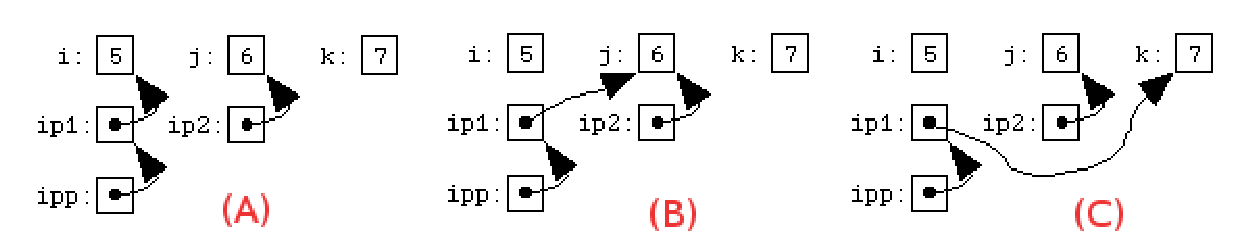
\includegraphics[height=2cm,
    angle=0]{./images/c_pointer.eps}}
\caption{(A) ; (B); (C); }
\label{fig:c-pointer}
\end{figure}

\begin{itemize}
\item [A] \verb!ipp! is the ptr-to-ptr, which hold the address of ip1.
\verb!*ipp! is the pointed pointer, \verb!**ipp! is the de-referenced twice variable. 

\begin{lstlisting}
ipp = &ip1;
\end{lstlisting}
\item [B] the content of the memory location that \verb!ipp!
  referencing to, which is the address of the memory location that
  \verb!ip1! is referencing to, change to the content of \verb!ip2!,
  which is the memory address that \verb!ip2! referencing to which
  hold the value of the variable $j$.
\begin{lstlisting}
*ipp = ip2;
\end{lstlisting}
\item [C] the content of the memory location that \verb!ipp!
  referencing to, which is the address of the memory location that
  \verb!ip1! is referencing to, change to the address of the memory
  holding the value for \verb!k!.
\begin{lstlisting}
*ipp = &k;
\end{lstlisting}
\end{itemize}


USAGE: This is widely used in C language as argument passing that allows the
function to modify the content value of the pointer
(Sect.\ref{sec:pointer-2Darrays}). In C++, it has passing by reference, so
passing a pointer to pointer is not the only option.

\begin{verbatim}
void func(int** ppInt)
{
  //Modify the pointer, ppInt points to
  *ppInt=&g_One;

  //You can also allocate memory, depending on your requirements
  *ppInt=new int;

  //Modify the variable, *ppInt points to
  **ppInt=3;
}
\end{verbatim}

% {\bf When to use pointers to pointers}:
% Let's see the simple example
% \begin{lstlisting}
% f(int *ip)
% {
%    *ip = 5;  // write to the location that ip points to the value 5
% }
% 
% ..........
% int i;
% f(&i);
% print (i);  // 5
% \end{lstlisting}
% It means that a function to return a value of type int, it used a
% parameter of type pointer-to-int.
% 
% Now, what if we want a function return a value of type pointer of
% string. 


\subsection{Reference to pointer (C++)}
\label{sec:reference-to-pointer}

Reference operator \verb!&! was added to C++98  (Sect.\ref{sec:&_operator})

\begin{verbatim}
//function prototype
void func(int*& rpInt);

int main()
{
  int nvar=2;
  int* pvar=&nvar;
  func(pvar);
  ....
  return 0;
}
\end{verbatim}

\url{http://www.codeproject.com/Articles/4894/Pointer-to-Pointer-and-Reference-to-Pointer}

\section{Dynamic memory allocation}
\label{sec:dynam-memory-alloc-1}

When working with pointers, it's important to know how to allocate memory
dynamically. You can dynamically allocate a region of memory and assign a
pointer to hold the memory address at which the newly created object resides.

Dynamic memory allocation is a very important part of most computer systems.
However, it can lead to memory leak if the dynamically allocated
memory is not freed properly at the end of the program.

\begin{enumerate}
  \item C98:  We will cover different ways to implement dynamic memory
  allocation in Sect.\ref{sec:understand_malloc}.

  \item C++ Boost library: Sect.\ref{sec:Boost::Pool}
\end{enumerate}

\subsection{Boost::Pool (C++)}
\label{sec:Boost::Pool}

Boost::Pool is often used when there is a lot of allocation and deallocation of
small objects.
\footnote{\url{http://www.boost.org/doc/libs/1_43_0/libs/pool/doc/index.html}}



\subsection{ANSI C: malloc() \& free()}
\label{sec:understand_malloc}

\begin{verbatim}
#include <stdlib.h>

void *malloc (size_t);
void free (void *);
void *calloc(size_t nmemb, size_t size);
void *realloc(void *ptr, size_t size);
void *reallocarray(void *ptr, size_t nmemb, size_t size);
       
\end{verbatim}
\url{http://man7.org/linux/man-pages/man3/malloc.3.html}


Early implementation of dynamic memory allocation was done by Doug Lea for C
language in 1987 as \verb!dlmalloc()! (dl means Doug Lea). This allocator
provides the basic implementation of the standard C routines: \verb!malloc(),
free(),! and \verb!realloc()!, as well as other auxiliary utility routines
\footnote{\url{http://gee.cs.oswego.edu/dl/html/malloc.html}}.
The dynamically allocated memory need to be free manually using \verb!free!
function. 

\textcolor{red}{Early malloc() is not thread-safe}: The \verb!malloc()!
allocates memory on a global heap (Sect.\ref{sec:heap_stack}), i.e. shared by
multiple threads, and it is possible that two different invocations of
\verb!malloc()! that happens at the same time, i.e. they can return the same
memory block when the second malloc call happen before the address of the chunk
is fetched, but the chunked is not marked as unavailable yet.

There is 3 main "versions" of C in ANSI C, C99 and C11
(Sect.\ref{sec:C11-intro}).
Since POSIX.1-2008 (Sect.\ref{sec:POSIX}), which is suported by C11,
\verb!malloc()! is thread-safe. Thread-safe implementation of \verb!malloc()!
uses a lock-based synchronization.
However, this still can cause deadlock when \verb!malloc()! is called from a
signal handler (Sect.\ref{sec:signal_handler}).

\begin{verbatim}
malloc();            //initial call
  lock(memory_lock); //acquire lock inside malloc implementation
signal_handler();    //interrupt and process signal
malloc();            //call malloc() inside signal handler
  lock(memory_lock); //try to acquire lock in malloc implementation
  // DEADLOCK!  We wait for release of memory_lock, but 
  // it won't be released because the original malloc call is interrupted
\end{verbatim}
So, the current implementation of \verb!malloc()! is thread-safe, but not
reentrant. None of the common versions of malloc allow you to reenter it (e.g.
from signal handler). 
\url{http://stackoverflow.com/questions/3941271/why-are-malloc-and-printf-said-as-non-reentrant}

To ensure signal handler safe:
\begin{enumerate}
  \item no dynamic memory allocation: avoid using malloc(), std::string,
  std::vector (which call malloc() internally)  
  
  \item  no buffered stdio or iostreams
\end{enumerate}

\subsection{C: malloc() or calloc()}
\label{sec:malloc()}
\label{sec:calloc()}

Allocating memory to be accessed by the CPU is most often accomplished using the
C standard library function malloc. If you have CUDA library, you can also
consider using cudaMallocHost() - Sect.\ref{sec:cudaMallocHost}.
 
We need to use the header file
\begin{enumerate}
  \item Linux: either  <stdlib.h> (in C) or <cstdlib> (in C++)
  \item Windows: <windows.h>
\end{enumerate}

\verb!calloc()! guarantees zero-initialize the buffers (clear-alloc) using
\verb!memset!, while \verb!malloc()! leaves the buffer uninitialized
(memory-alloc). 

As zeroing out the memory takes sometimes, if you want it fast, and zero-value
is not important, and you should consider using \verb!malloc()!.
The memory is allocated on heap (Sect.\ref{sec:heap_stack}).

IMPORTANT: The returned pointer is not a constant pointer, so we can change its
pointing address. However, we will no longer pass that pointer to the
\verb!free! function as it wont point to the first byte any more. So, it's
important to treat that pointer as a constant, i.e. don't change it.

\textcolor{red}{Another important but less known difference is that in some O/S
with optimistic memory allocations, e.g. Linux, the pointer returned by malloc()
is not backed by real memory until the program actually touches it. As calloc()
set the zero values, the O/S sure is backing the allocation with actual RAM or
swap}. So, calloc() is slow not only it set the values, but also it needs to
find a suitable memory area by possibly swapping out other processes.

A rather often-overlooked advantages of \verb!calloc()! is that it make sures
to avoid overflow
\begin{verbatim}
// overflow occurs if 'count' > SIZE_MAX/sizeof(*bar)
size_t count = get_int32(file);
struct foo *bar = malloc(count * sizeof *bar);
\end{verbatim}
\url{http://stackoverflow.com/questions/1538420/difference-between-malloc-and-calloc}


A generic pointer \verb!void*! pointing to the first byte of memory allocated is
returned, which can be mapped to any other poniter type.
\begin{lstlisting}
#include <stdlib.h>

double *dptr = malloc(n* sizeof(double));

if (dptr == NULL) printf("cannot allocate")
else free(dptr);
\end{lstlisting}

\verb!malloc! return a generic pointer to the first byte of the
allocated memory. Even though we assign a generic pointer to a double
pointer, we don't need to use type cast as in this case, it is
automatically managed by C compiler. However, you can also do it explicitly 

\begin{lstlisting}
double *dptr = (double *) malloc(n* sizeof(double));
if (dptr != 0) {
   /* success, do it */
?
\end{lstlisting}
If the task is failed (for some reason), it returns a NULL pointer. {\bf NOTE}:
\textcolor{red}{Always check the successfullness of }\verb!malloc!.

{\bf NOTE}: When allocating an array of zero element, \verb!malloc(0)!, the
result is implementation defined, which can be either a NULL pointer or an
address. We don't want it to return NULL for two reasons: (1) we want to use
NULL return as a sign that malloc() has failed, (2) we want a unique pointer for each
call to malloc() so that we can add it to the block table.
\begin{verbatim}
    void * ptr;
    ptr = malloc(0);
    free(ptr);
\end{verbatim}
To work arround, a suggested user-defined implementation to check for zero-size
and always allocate at least sizeof(void*). NOTE: Here we consider
MPI-application. However, using this can slow down the performance. That's why
we can define a macro \verb!FAST_MALLOC! to use when compiling the code.

{\small \begin{verbatim}
#ifdef FAST_MALLOC
  #define ddcMalloc(size)      malloc(size)
#lse


#define ddcMalloc(size) _ddcMalloc(size, __ddcLine(__FILE, __LINE))

void* _ddcMalloc(size_t size, char* location)
{
	if (size == 0) size=sizeof(void*);
	void *ptr = malloc(size);
	if (!ptr){
	  printf(``Mem-allocate failed on task %d (%zu bytes at %s)\n''
	         ``                        memUsed=%8.2f\n'', 
	         getRank(0), size, location, _memUd/b2mb)
	  printHeapInfo(stdout);
	}else{
	   int b = addBlock(ptr, size, location);
	}
	return ptr;
}}
\end{verbatim}}


{\bf calloc()}: The data allocated by \verb!malloc! is not guaranteed to be
initialized to any value. So, a variant is \verb!calloc! that automatically
initialize the data to zeros.

\begin{lstlisting}
type * pData;
pData = calloc(unsigned int num, size_t sizeof(type))
\end{lstlisting}

We can allocate memory for a structure
\begin{verbatim}
#include <stdlib.h>
#include <stdio.h>

typedef struct rec{
  int i;
  float PI;
  char A;
} RECORD;

struct rec2{
  int i;
  float PI;
  char A;
}

int main() {
  RECORD *ptr_one;
  ptr_one = (RECORD*) malloc(sizeof(RECORD));

  struct rec2 *ptr_two;
  ptr_two = (struct rec2 *) malloc(sizeof(struct rec2)); 
  ...

  printf ("First value %d\n", (*ptr_one).i);
  printf ("Second value %f\n", ptr_one->PI);  
  free(ptr_one);
  free(ptr_two);
  return 0; 
}
\end{verbatim}
NOTE: There are two ways to access a data element of a pointer. Most people use
\verb!->! operator.

NOTE: When allocating a string \verb!char*!, always add 1 to the expected string
length.
\begin{verbatim}
int strlen = 10;
char * str;

alloc(str, sizeof(*str) * (strlen+1));
\end{verbatim}

\subsection{C: realloc()}
\label{sec:realloc()}

\verb!realloc(ptr, size)!
\begin{verbatim}
void* realloc (void* ptr, size_t size)
\end{verbatim}
\begin{itemize}
  \item C90 (C++98): if the size is zero, then the memory previously allocated
  for \verb!ptr! is freed using \verb!free()! and a NULL pointer is returned.
  \item C99/C11 (C++11): depend on the particular library implementation, which
  can be either a NULL pointer, or a pointer to some other location that shall
  not be dereferenced.
\end{itemize}
Other situations:
\begin{enumerate}
  \item  If \verb!size! is not zero, and the function fails to allocate the requested
block of memory, a NULL pointer is returned, while the memory pointed by
\verb!ptr! is unchanged. If the function is success,  the function return a
pointer to the memory block allocated by the function.
  \item If the new size if bigger, the value of the newly allocated portion is
  indetermine.
  \item If \verb!ptr! is a NULL pointer, the behavior is like \verb!malloc()!.
\end{enumerate}

A suggested approach: it's best to store the return value in a temporary
variable. If \verb!realloc()! fails, e.g. not enough memory, then it returns
NULL, while the original pointers is NOT freed. So, it's better not to change
the address of the original before knowing what's really happening
\begin{verbatim}
char *tmp = realloc(result, newsize);
if (tmp == NULL)
{
    // handle error here and free the memory
    free(result);
}
else
{
    // reallocation was successful, re-assign the original pointer
    result = tmp;
}
\end{verbatim}

\subsection{C: xalloc()}
\label{sec:xalloc()}

\subsection{C: alloca() on stack}
\label{sec:alloca()}

For small-size array with unknown size at compile time, we can use
\verb!alloca()! to allocate the memory on stack (Sect.\ref{sec:heap_stack}).
Here, the memory is automatically freed when the calling function exit. So,
there is no need to call \verb!free()!.  This is often used with array
(Sect.\ref{sec:alloca}).


\subsection{C: free() and dangling pointer}
\label{sec:free()}

{\bf NOTE}: \verb!free()! only works with dynamically allocated pointers
(Sect.\ref{sec:dynam-memory-alloc-1}), not with global or static pointers.

When you have two pointers pointing to the same memory location, and you free
that memory allocation, the second pointer becomes a dangling pointer, i.e. a
pointer that point to an invalid memory.

\begin{verbatim}
char* ptr = malloc(100);
...
free(ptr);
ptr = NULL;
\end{verbatim}
Then, later on, if you accidently free a NULL pointer, the O/S silently does
nothing.

\subsection{using macros for debugging purpose}

ANSI C preprocessor will replace the special symbols \verb!__FILE__! and
\verb!__LINE__! with the file and line number of the macro's invocation

\begin{verbatim}
void *malloc (size_t);
void *_malloc_leap (const char *file, int line, size_t size);
#define malloc(size) _malloc_leap(__FILE__, __LINE__, size)

void free (void *);
void _free_leap (const char *file, int line, void *);
#define free(ptr) _free_leap (__FILE__, __LINE__, ptr);

\end{verbatim}



\section{Type cast}
\label{sec:type-cast}

Typecasting is the concept of converting the value of one type into another type
(type conversion). The conversion can be implicit (i.e. done automatically by
the compiler), or explicit (i.e. the target type is coded in by the programmer).

There are three types of explicit conversion.
\begin{enumerate}
  \item {\bf checked} : prechecked at runtime before the conversion. If the
  destination type cannot hold the source value, an error is raised. 
  
  \item {\bf unchecked}: no checked is performend. If the destination type
  cannot hold the source value, the result is {\it undefined}. 
  
  \item {\bf bit pattern}:  the data is not interpreted at all, i.e. the raw-bit
  representation of the source is copied, and then re-interpreted according to
  the new type. 
\end{enumerate}

The C/C++ type-cast is either ``unchecked'' or ``bit pattern''
\begin{itemize}

  \item C style - Sect.\ref{sec:type-cast-C}: \verb!(new_type)expression!

\begin{lstlisting}
class A;
class Asub: public A;

A* ptr = new Asub();

Asub& b = (Asub)ptr;

// or 
float fl = 5.4;
int ii = (int) fl; 
\end{lstlisting}  

  \item C++ style: It uses one of the following syntax
  
\begin{Verbatim}
new_type(expression)
    
dynamic_cast <new_type> (expression)
reinterpret_cast <new_type> (expression)
static_cast <new_type> (expression)
const_cast <new_type> (expression)
 \end{Verbatim}
\end{itemize}


\subsection{In C}
\label{sec:type-cast-C}

With implicit type-casting, typically, the compiler will issue a warning for
each implicit conversion it does. An example is 
\begin{verbatim}
int i_value   = 16777217;
float f_value = 16777216.0;
    
if (i_value > 2) i_value = f_value; /* implicit */    
\end{verbatim}

then the warning can be
\begin{verbatim}
conversion from 'double' to 'int', possible loss of data.
\end{verbatim}

Usually, the compiler do type cast promotion in the order for the intrinsic data
type
\begin{verbatim}
int -> unsigned int -> long -> unsigned long -> long long -> 
unsigned long long -> float -> double -> long double
\end{verbatim}

\subsection{--   (T)somevariable}

\textcolor{red}{However, it's considered a good programming practice to use
explicit type casting with {\bf cast operator}}, i.e.
the target type is wrapped inside the parantheses, \verb!(T)expression!.
\begin{verbatim}
some_type b;
type_name a;

a = (type_name) b;
\end{verbatim}


Example:
\begin{verbatim}
double da = 3.3;
double db = 3.3;
double dc = 3.4;
int result = (int)da + (int)db + (int)dc; //result == 9
\end{verbatim} 

One use for type cast is to use ASCII characters
\begin{verbatim}
    for ( int x = 0; x < 128; x++ ) {
        /* Note the use of the int version of x to output a number and the use
         * of (char) to typecast the x into a character which outputs the
         * ASCII character that corresponds to the current number
         */
        printf( "%d = %c\n", x, (char)x );
    }
    getchar();
\end{verbatim}

In C, the compiler doesn't detect errors like this. C-stype cast allows an INT
pointer to point to a CHAR pointer.
\begin{verbatim}
char c = 10;       // 1 byte
int *p = (int*)&c; // 4 bytes
\end{verbatim}

Writing to 4-byte pointer will either cause run-time error or overwrite adjacent
memory, as the compiler doesn't check for data type compatibility. 
\begin{verbatim}
*p = 5; /* potential error */
\end{verbatim}


\subsection{In C++}
\label{sec:type-cast-C++}

We can still use C-style in C++; yet it's suggested to use C++ style which
utilizes {\it explicit type conversion}. C++ provides 4 different ways of
type-cast
\begin{Verbatim}
new_type(expression)
    
dynamic_cast <new_type> (expression)
reinterpret_cast <new_type> (expression)
static_cast <new_type> (expression)
const_cast <new_type> (expression)
 \end{Verbatim}

NOTE:
\begin{Verbatim}
MyClass *m = (MyClass *)ptr;  // C-style
           = MyClass* (ptr); // C++-style

           = const_cast<MyClass *> ptr; 
           = static_cast<MyClass *>(ptr);  // recommended: C++-style 
           = static_cast<MyClass *> (const_cast<MyClass *>)ptr;
           
MyClass *m = reinterpret_cast<MyClass *> ptr;
           = reinterpret_cast<MyClass *> (const_cast<MyClass *>)ptr;
MyClass *m = dynamic_cast<MyClass *>(ptr); // C++-style
\end{Verbatim}

\subsection{-- T(somevariable)}

The C style \verb!(T)something! and the C++ style \verb!T(something)! are
equivalent for type cast and both should be avoided in C++; the latter one
(C-style) should be avoided more.  IMPORTANT: Using C++-style for a class
object, the downcast also strips off \verb!const!-property if the original
pointer is marked with \verb!const! attribute (to preserve this, use
\verb!static_cast! - Sect.\ref{sec:static_cast}).


In C++, with class (object-oriented) and inheritance, it's getting more
important to understand type-casting. There are two ways: downcasting and
upcasting.
\begin{itemize}
  \item Upcasting: convert a derived-class reference or pointer to a base-class.
  This allows us to treat the object of the derived-class as if it was of the
  base-class type. \textcolor{red}{This is always allowed for {\bf public}
  inheritance} (Sect.\ref{sec:inheritance_public}).  We are allowed to use
  implicit type-cast. Upcasting can cause \textcolor{red}{\it object slicing}
  when the object of derived-class is passed by value as a base-class object
  (Sect.\ref{sec:object-slicing}).
  
  \item Downcasting: convert a base-class reference or pointer to a
  derived-class. Explicit type-cast is required. 
\end{itemize}


A type-cast like this
\begin{verbatim}
T* ptr = (T*) var;
\end{verbatim}
doesn't tell right away, in C++, if 
\begin{enumerate}
  \item a cast is from a base class to a derived class or the other way around
  \item a cast stripes the constant object \verb!const! or not
  \item a cast is from an integral type to a pointer or not 
\end{enumerate}

To help making it clear and to improve safety, C++11 provides new syntax. The 4
new different typecast operators all use angle brackets \verb!< ... >! and put the target type inside
\begin{enumerate}
  \item \verb!static_cast!
  \item \verb!reinterpret_cast!
  \item \verb!const_cast!
  \item \verb!dynamic_cast!
\end{enumerate}
Using one the 4 above syntax, C++ style type cast are checked
by the compiler. Each cast handles one specific sort
of convention or a family of related conversions. This allows the compiler to go on
and check that you're not accidentally doing something that you are not
intended.


\subsection{-- static\_cast}
\label{sec:static_cast}

\verb!static_cast! is used for type-casting, while maintaining the
const-attribute. 

Example of the C-style cast problem: You have the code
\begin{verbatim}
void DoSomething(Base* ptr) {
    Derived* derived = (Derived *) (ptr);
    DoSomethingElse(derived);
}
\end{verbatim}
and now you don't want to make change to the content of the object pointed to
by \verb!ptr!, so you want to emphasize to mark the argument with \verb!const!
(see Sect.\ref{sec:const_its-position})

\begin{verbatim}
void DoSomething(Base const * ptr) {
    Derived* derived = (Derived *) (ptr);
    DoSomethingElse(derived);
}
\end{verbatim}

However, now it is the problem. Using C-style the downcast also strips off
\verb!const!-property. This is an easily bug if DoSomethingElse() method really
modify the input. If your code is
\begin{verbatim}
void DoSomething(Base const * ptr) {
    Derived* derived = static_cast<Derived *>(ptr);
    DoSomethingElse(derived);
}
\end{verbatim}
which keep the \verb!const!ness property of \verb!ptr! and pass to
\verb!derived!. Thus, the compiler error is raised if \verb!derived! is modified
inside DoSomethingElse().

\begin{mdframed}

In C++, \verb!static_cast<>()! does two things 
\begin{enumerate}
  \item casting to the new type while keeping the existing property of the
  original object (e.g. \verb!const!ness if possible), 
  
  \item make sure the type conversion is compatible. Thus, using
  \verb!static_cast<>! is a safer way as it gives compile time checking
  capability, which is not available in C (see above).  
\end{enumerate}

\end{mdframed}

\begin{verbatim}
char c = 10;
int *q = static_cast<int*>(&c); // compile-time error detection
\end{verbatim}

So, the compiler will check for type compatible. Also, using it is more
readable, and can spot easily inside a C++ code. It's widely used for conversion
from derived class to base class (i.e. inheritance
Sect.\ref{sec:OO_inheritance}). \textcolor{red}{This is the first cast you
should attempt to use, i.e. if we know that the pointer is actually pointing to
an object of a specific type}. 

IMPORTANT: It's possible to map \verb!const! objects to non-const objects
(Sect.\ref{sec:const_C++}): read \verb!const_cast<>!
(Sect.\ref{sec:const_cast}).

Example:
\begin{verbatim}
	enum my_numbers { a=10, c=100, e=1000 };

	const my_numbers b = static_cast<my_numbers> (50);
	const my_numbers d = static_cast<my_numbers> (500);
\end{verbatim}

\subsection{-- const\_cast}
\label{sec:const_cast}

In C++, if the original object being casted has \verb!const! property or
\verb!volatile! property, you can cast that propery away from the object, i.e.
assign to a pointer in that the memory can be modified via that pointer.
Because of this, it's recommended NOT to use \verb!const_cast<>! as it reveals
(most of the time) a flaw in the design, i.e. a not-supposed-to-be-modified
data now become modifiable-data.

\begin{verbatim}
void a(Person* b);

	int main()
	{
		const Person *ptr_my = new Person("Joe");
		a( const_cast<Person *>(ptr_my) );
	}

\end{verbatim}


We only NEED to use this when we want to interface a C++ code with an existing
C-code. The reason is that a lot of C code use \verb!char*! as arguments even
when the string is not modified, whereas in C++ it should be used as \verb!char!
\verb!const *! or \verb!const char*!.  The mismatch between C++ and C can be
resolved by using \verb!const_cast<>!. First, make sure the code you're trying
to hook is not trying to modify the data you're passing in. Then, as in C++ we
already design such object as \verb!const! (or \verb!volatile!) and we need to
pass it to the C function, that accepts an object without \verb!const! property
(or \verb!volatile!), then we use \verb!const_cast! first to remove this
attribute before passing to the function that accept non-const pointer (but
make sure the function does not modify the data).

\subsection{-- dynamic\_cast}
\label{sec:dynamic_cast}

In C++, \verb!dynamic_cast<>()! is used when we don't know what the dynamic type
of the object is, by checking with a give type. Dynamic cast return a NULL
pointer if the object referred to doesn't contain the type casted as the base
class 

\begin{verbatim}
if(JumpStm *j = dynamic_cast<JumpStm*>(&stm)) {
  ...
} else if(ExprStm *e = dynamic_cast<ExprStm*>(&stm)) {
  ...
}
\end{verbatim}

\subsection{-- reinterpret\_cast}
\label{sec:reinterpret_cast}


Example:
\begin{verbatim}
int *ptr;
ptr = malloc(10 * sizeof (*ptr));		/* without a cast */
ptr = (int *)malloc(10 * sizeof (*ptr));	/* with a cast */
ptr = reinterpret_cast<int *>(malloc(10 * sizeof (*ptr))); /* with a cast, for C++ */
\end{verbatim}


In C++, using \verb!interpret_cast<>! is almost as dangerous as the old-fashon
C-style cast, as it allows mapping from one type to ANY type without checking at
compile-time. The only difference is that it guarantees (detectable at
compile-time) you cannot cast a \verb!const! object to a non-const object.

Example:
\begin{verbatim}
D* d = nullptr;
//  A* a = (A*)d;                   // compile-time error

A* a = reinterpret_cast<A*>(d); // this compiles (but will crash at runtime)
\end{verbatim}

Example:
\begin{verbatim}
char *const MY = 0;

	// This is not valid because MY is a const!!
	int *ptr_my = reinterpret_cast<int *>( MY);
\end{verbatim}

\subsection{In C++/CLI}

C++/CLI from Windows also provide \verb!safe_cast!

\subsection{Tips}

NOTE: In an expression, we needs to wrap the object inside the parentheses as
well. It's recommended to do this all the times
\begin{verbatim}
double out;
int a=10; 
int b = 5;

out = static_case<double>(a)/b;
\end{verbatim}


\section{Print address}
\label{sec:print-address}

You can print the memory address of a variable using \verb!%p! option
if the \verb!printf! command.
\begin{lstlisting}
int i = 10;
printf("&i=%p\n", (void*) &i);
\end{lstlisting}

\section{Increment a pointer}

We can increase the memory address 

\begin{verbatim}
int *p;
int a = 100;
p = &a;
\end{verbatim}

For a pointer, an increment is similar to an array
\begin{verbatim}
p++;
\end{verbatim}
However, it's important to know that in a normal increment, the value added is
1. For the case of a pointer, the value added is the size of the memory element
it's pointing to. So if it's an \verb!int! pointer, then the value added is 4.

\section{Size of an array (sizeof)}

NOTE: \verb!sizeof! returns the number of storage in BYTES.

First, we allocate an array of 'n' elements, whose element is a \verb!mystruct!
struct.
\begin{verbatim}
if (NULL == (array = calloc(sizeof(struct mystruct) * n,1))) {
 /* handle error */
}
\end{verbatim}

Even though \verb!malloc()! keeps track of how much memory is allocated and
\verb!free()! should know how much memory it needs to free. Unfortunatelly,
there is no way to get the size information in C, as \verb!malloc()! may
allocate more bytes than you request (e.g. for efficiency purpose). Ideally, you
need to keep track of 'n', 

If we have the statistically allocated array (array pointer), then we can do
\begin{verbatim}
#define MAX_DATA 10
mystruct* data[MAX_DATA];//array of pointers to aliasID

int length =  sizeof array / sizeof array[0];
\end{verbatim}

However, if we only have the pointer to the first element, it's impossible to
get the real length.
\begin{verbatim}
 mystruct* pchar = array;
\end{verbatim}


References:
\begin{enumerate}
  \item
  \url{http://stackoverflow.com/questions/15774534/c-how-to-get-the-length-of-a-pointer-array}
\end{enumerate}
\section{Potential mistakes}
\label{sec:potential-mistakes}

\subsection{Reset array}

It's recommended to reset the array with all values get zeroes, instead of
garbage value.

\begin{lstlisting}
int arraySize = 20;
int a[arraySize];

int value_to_set = 0;

std::memset(a, value_to_set, sizeof(int)*arraySize);
\end{lstlisting}
Here, the number of bytes is passed in.

In C++, we can use
\begin{lstlisting}
template<class ForwardIt, class T>
void fill(ForwardIt first, ForwardIt last, const T& value);
template<class OutputIt, class Size, class T>
OutputIt fill_n(OutputIt first, Size count, const T& value);
\end{lstlisting}
We give it an iterator to start at, we tell it how many elements (NOT the
number of bytes) we will visit, and we pass it a value.

Advantage: it is not limited to pointers anymore; we can do a \verb!std::fill!
on a linked list and the call site will look exactly the same as a call to do the
same thing on a vector or an array.

Example:
\begin{lstlisting}
struct GroceryItem {
  string name;
  double price;
};

void tomatoesEverywhere(vector<GroceryItem>& inventory) {
  GroceryItem tomatoes { "tomatoes", 2.0 };
  
  //Everything is a tomato now! (Muahahahaha)
  std::fill(begin(inventory), end(inventory), tomatoes);
}
\end{lstlisting}

\url{http://maintainablecode.logdown.com/posts/159916-memcpy-memmove-and-memset-are-deprecated}
\subsection{Array assignment vs. Array copy}
\label{sec:array-assignment}

As an array is indeed a pointer to a memory location, using assignment (=)
simply changes the memory location referenced by that pointer.

\textcolor{red}{WRONG}: If you want to make a copy of a given array to another
array, doing this is a mistake
\begin{lstlisting}
double f[MAXVALS], g[MAXVALS];

f = g;    // illegal
\end{lstlisting}
This operations indeed $f$ point to $g$, or the memory location of $f$
and $g$ will be the same.  As both $f$ and $g$ are array names, they
are {\bf constant pointer}s. It means that they cannot change the
memory location. Thus it is illegal.

\section{Copy memory using pointers}
\label{sec:array-copy}

To do array copy (vector copy) in C/C++,  there are a few functions that allows
us to do the job
\begin{enumerate}
  \item for array of primitive data type (int, float): \verb!memmove()! or
  \verb!memcpy! are fast, but no memory overlapping check.
  
  For fundamental types like int, the bitwise copy done by memcpy will work
  fine. For actual class instances, you need to use std::copy (or \verb!std::copy_n!) so
  that the class's customized assignment operator will be used.
  
  \item \verb!std::copy!: Sect.\ref{sec:std::copy}
 
  \item \verb!std::copy_n!
\end{enumerate}


NOTICE: These functions accept void pointers
\begin{itemize}
  \item \verb!bcopy()! : a POSIX's deprecated function, like memmove() but with
  swapped sources
  
  \item \verb!memcpy()!: a GNU function, like memcpy(), and also returns a
  pointer to the byte after the last byte written
  
  \item \verb!memccpy()! (POSIX), \verb!_memccpy()! (Microsoft): can stop the
  copy on selected value; otherwise identical to memcpy()
  
  \item \verb!g_memmove()! (GNOME):a macro that usually maps to memmove()
  
  \item \verb!CopyMemory(), MoveMemory()! (Microsoft): identical to memcpy() and
  memmove()
  
  \item \verb!memcpy_s(), memmove_s()! (Microsoft): add destination array
  length, and array bound checking; otherwise identical to memcpy() and
  memmove().
  
  \item 
\end{itemize}

Wide-character pointers:
\begin{enumerate}
  \item \verb!wmemcpy()! (ISO C), \verb!wmemmove()! (ISO C), \verb!wmemcpy()!
  (GNU): wide character pointer arguments, but are otherwise identical to
  memcpy( ), memmove( ), and mempcpy( ).
  
  \item \verb!wmemcpy_s()!, \verb!wmemmove_s()! (Microsoft): add destination array
  length, and array bound checking; otherwise identical to \verb!wmemcpy()! and
  \verb!wmemmove()!
  
\end{enumerate}

\subsection{mem* function (memcpy, memmove) vs. std::copy, std::fill,
std::equal}

The mem* family of functions should not be used nowadays.
As std::copy, std::move, std::fill, and std::equal provide type-safe, more
general, and equally efficient interfaces to perform the same tasks as
std::memcpy, std::memmove, std::memset, std::memcmp, and their wide variants.

\begin{lstlisting}
void* memcpy(void* dest, const void* src, std::size_t count);
void* memmove(void* dest, const void* src, std::size_t count);
void* memset(void* dest, int value, std::size_t count);
int memcmp(const void* lhs, const void* rhs, std::size_t count);
\end{lstlisting}
\url{http://maintainablecode.logdown.com/posts/159916-memcpy-memmove-and-memset-are-deprecated}





\subsection{memcpy()}
\label{sec:memcpy()}

 \verb!memcpy()!: no check for overlapping
  
Defined in <string.h> (which is included inside <memory.h>, <cstring>
(C++-compatible version))
\begin{lstlisting}
memcpy( (void*)dst, (void*)src, n * sizeof(int) );
\end{lstlisting}

However this requires there is no memory overlap between the two arrays.
\begin{lstlisting}
/*syntax*/
void * memcpy ( void * destination, const void * source, 
                size_t num );

// example:
memcpy(f, g, sizeof(g));
\end{lstlisting}
with $num$ is the number of bytes to copy.  If there are memory
overlap between the two arrays, a safer approach is to use
\verb!memmove!. For non-overlap arrays, \verb!memcpy! works more
efficient. 

\subsection{memmove}
\label{sec:memmove}

\verb!memmove()!: for copying memory,  with check for overlapping.
It spends some time determining how and whether the source and target overlap,
so it can decide the order in which to copy the data.
\begin{itemize}
  \item if overlap on the beginning-side
\begin{verbatim}
          source-----------
dest---------
\end{verbatim}
then copy forward.

  \item if overlap on the end-side
\begin{verbatim}
source-----------
          dest---------
\end{verbatim}
then copy backward.

\end{itemize}
The time memmove() spends doing the initial calculation is, for moves of
reasonable size, likely to be a small fraction of the time spent copying the data.
\url{http://stackoverflow.com/questions/23122280/what-is-memmove-alternative-when-i-know-the-overlapping-side}

\begin{lstlisting}
void *memmove(void* dest, 
             const void* source, 
             size_t len) // copy with overlap possible
\end{lstlisting}  
NOTE: The function does not check for any terminating null character in source -
it always copies exactly \verb!len! bytes.

\subsection{std::copy\_n}
\label{sec:std::copy_n}

\verb!std::copy_n! (C++11, <algorithm> header file) (fastest):
  which is a template and accepts any data type
\begin{verbatim}
n = 7;
std::copy_n ( myints, n, myvector.begin() );
\end{verbatim}    
If $n$ is negative, it does nothing. If ranges overlapped, the elements in the
result may get undefined (but valid) values. It also returns an iterator point
to the value past the last element copied.
\url{http://www.cplusplus.com/reference/algorithm/copy_n/} 


\subsection{std::copy}
\label{sec:std::copy}

\verb!std::copy(src_from, src_to, dest_start)! (<algorithm> header file) 
\begin{itemize}
  
   \item Older version uses a for-loop to copy every elements in the range
   \verb![from, to)! to \verb!dest! location, one by one which is slow.
   
     
   \item Newer version: use template-based implementation, and call system
   function for copying an array of primitive data
   
   \verb!std::copy()! is the best as it knows when to use memcpy() and 
   when to use memmove().

%\verb!std::copy!  (fastest):  which is a template and accepts any data type
\begin{verbatim}
template<class InputIterator, class OutputIterator>
  OutputIterator copy (InputIterator first, InputIterator last, OutputIterator result)
\end{verbatim}
   
\end{itemize}



Example:
\begin{lstlisting}
#include <algorithm>    // std::copy
#include <vector>       // std::vector

void main()
{
  int myints[] = {10,20,30,40,50,60,70};
  std::vector<int> myvector (7);

  std::copy ( myints, myints+7, myvector.begin() );
  return 0;
}
\end{lstlisting}

Benchmark: \url{http://stackoverflow.com/questions/4707012/c-memcpy-vs-stdcopy}

\subsection{get/set}

using get/set
\begin{lstlisting}
for ( size_t i = 0; i < n; ++i )
	set( dst, i, get( src, i ) );

int get( const int*const src, const size_t index ) { return src[index]; }
int set( int*const dst, const size_t index, const int value ) { dst[index] = value; }
\end{lstlisting}

\url{http://nadeausoftware.com/articles/2012/05/c_c_tip_how_copy_memory_quickly}

\subsection{std::fill, std::fill\_n}
\label{sec:std::fill}

This fills a number of elements in a container the same values
\begin{lstlisting}
template<class ForwardIt, class T>
void fill(ForwardIt first, ForwardIt last, const T& value);

template<class OutputIt, class Size, class T>
OutputIt fill_n(OutputIt first, Size count, const T& value);
\end{lstlisting}

\subsection{memset}
\label{sec:memset}

Example: set all elements in array \verb!a! (first argument) with the same value
passed on as the second argument
\begin{lstlisting}
int arraySize = 20;
int a[arraySize];
std::memset(a, 0, sizeof(int)*arraySize);
\end{lstlisting}

A better option is to use \verb!std::fill!, \verb!std::fill_n!
(Sect.\ref{sec:std::fill})

\begin{lstlisting}
int memcmp(s1, s2, n)  ! return (-), 0, (+) if first n bytes
  ! of s1 is <, ==, > than first n bytes of s2
void *memchr(s, c, n)  ! return the pointer to the first
  ! occurrence of c in first n bytes of s
void *memset(d, c, n)  ! return d, copy c into the first
  ! n bytes of d
\end{lstlisting}


\subsection{String copy}
\label{sec:string-copy}

We can use the methods in Sect.\ref{sec:array-copy}, and treat it as a void
pointer, but there are also methods for character-array

Character pointers
\begin{enumerate}

  \item \verb!strncpy()! (ISO C), \verb!stpncpy()! (GNU): copy and stop at the
  first \verb!'\0'! character; otherwise identical to memcpy() and mempcpy()
  
  \item \verb!strncpy_s()! (Microsoft): add destination array
  length, and array bound checking; otherwise identical to \verb!strncpy()!
  
  \item \verb!strcpy()! (ISO C): requires the target memory needs to be
  pre-allocated
  
\begin{lstlisting}
strcpy(ptr2, ptr1) 
\end{lstlisting}  
is equivalent to \verb!while(*ptr2++ = *ptr1++)!

  \item \verb!strdup()! (POSIX): the target memory is not necessary to be
  pre-allocated as it will be (re)allocated implicitly
  
\verb!strdup(ptr2, ptr1)! is equivalent to  
\begin{lstlisting}
ptr2 = malloc(strlen(ptr1)+1);
strcpy(ptr2,ptr1);
\end{lstlisting}  
use this if you want the string to be created is in the heap (so that it can be
used in a different place)


\end{enumerate}

Wide-character pointers:
\begin{enumerate}
  \item \verb!wcsncpy()! (ISO C), \verb!wcpncpy()! (GNU): wide character pointer arguments
  and stop the copy at the first \verb!'\0'! wide character, but are otherwise
  identical to strncpy() and stpncpy()
  
  \item \verb!wcsncpy_s()! (Microsoft): add destination
  array length, and array bound checking; otherwise identical to
  \verb!wcsncpy()!.
  
\end{enumerate}
\chapter{C++ Pointers}

\section{::operator new, ::operator new[]}

\subsection{C++: notice}

In C++, we can allocate raw memory using the C-based functions (malloc(),
calloc(), \ldots - Sect.\ref{sec:malloc()}) for backward compatibility.
In C++ compiler, the header file to those functions is \verb!<cstdlib>!.


However, these C-based functions return a generic pointer \verb!void*!. The lack
of a specific pointer type returned is considered as type-unsafe by many
programmers. Also, the allocation is based on number of bytes, not the number of
objects or data elements, which is not straight forward convention in C++.  

\begin{mdframed}

For backward compatibility with C code, to dynamically allocate memory, in C++,
we can use C functions,  \verb!malloc!, \verb!calloc!, \verb!realloc! and
\verb!free! by including the <cstdlib> header file (Sect.\ref{sec:malloc()}).

However, it is important to know that C++ does not allow implicit type-cast;
instead, programmers need to call dynamic-cast function to cast from
\verb!void*! to a specific type.

\end{mdframed}


As C++ is a strong-type language, so type-casting is always recommended.
In C++, it's more convenient to think the number of dynamically objects, rather
than the total number of bytes all these objects occupy.

C++ languages thus provides a few new functions to allocate/free memory, e.g.
new or new[], delete or delete[]. Sect.\ref{sec:operator-new-C++}).

Also, C++ DOES NOT allow implicit casts from void * to other pointer types.
This prevents most C code from compiling under a C++ compiler, particularly if
the C code contains calls to malloc(). To resolve that issue, C++ introduced some
new operators for dynamic type-casts (Sect.\ref{sec:type-cast-C++}) such as 
\verb!reinterpret_cast! (Sect.\ref{sec:reinterpret_cast}).

 
\subsection{C++11: new operator  vs. ::operator new(...) }
\label{sec:new-operator}

C++ supports dynamic allocation of objects using the \verb!new! operator. The \verb!new!
operator allocate memory for objects from a pool called the free store. Behind the scene, the new
operator calls the special function \verb!::operator new! (Sect.\ref{sec:operator-new-C++}).
 
Example: \verb!new! operator allocate one object, which may takes a few number
of bytes.
The 'new' expression which knows how many bytes it needs, then pass that value
to 'operator new' to allocate raw memory, then after that, it evokes the object's constructor next.

\begin{verbatim}
Apple * p = new Apple(); //new expression using the constructor Apple()
 
Apple * p = new Apple("gala"); //new expression using the constructor Apple(std::string)

\end{verbatim}

  
%\section{C++: 'new' operator}
\subsection{::operator new (C++)}
\label{sec:operator-new-C++}


SYNTAX: We optionally can use \verb!::! at the front which explicitly referring to the global-scope operator 
\verb!new!.
\begin{verbatim}
#include <new>

[::] "new" ["(" expression-list ")"] {new-type-id | "(" type-id ")"} ["(" expression-list ")"]
[::] "delete" ["[]"] cast-expression

void *operator new (size_t);
void operator delete (void *);
void *operator new[] (size_t);      // for arays
void operator delete[] (void *);
\end{verbatim}

\verb!::operator new! below just allocate raw memory, by telling it the number
of bytes; and no object's constructor is called [which is evoked by the new
operator] (Sect.\ref{sec:new-operator}).

\begin{verbatim}
void* mem = operator new(sizeof(apple)); //just like calling malloc()
// or
// void* mem = ::operator new(sizeof(apple)); //just like calling malloc()

//now the constructor is next

apple* p2 = new(mem) apple(1); //call construct here using placement new.

 \end{verbatim}

\url{https://stackoverflow.com/questions/1885849/difference-between-new-operator-and-operator-new} 


\url{https://en.cppreference.com/w/cpp/header/new}


\begin{verbatim}
https://en.cppreference.com/w/cpp/memory/new/operator_new

void* operator new  ( std::size_t count );
void* operator new[]( std::size_t count );


(since C++17)
void* operator new  ( std::size_t count, std::align_val_t al);
void* operator new[]( std::size_t count, std::align_val_t al);
\end{verbatim}

This is different from the \verb!new! operator.

So, it is recommended to use the \verb!new! operator in C++ -


\subsection{-- usecase 01}

C++ provides a \verb!new! operator to create a pointer to an
object, or an array of object. If the
allocation fails, it throws an exception of type \verb!std::bad_alloc!, i.e. we
don't need to check for the result.

To avoid throwing exception, i.e. if it fails, return a NULL pointer and
continue the execution, we use a special object called \verb!nothrow! declared
in header file \verb!<new>!. 

\begin{verbatim}
#include <new>

bobby = new (nothrow) int [5]; 
if (bobby == 0) {
  // error assigning memory. Take measures.
  }; 
\end{verbatim}

NOTICE: \verb!nothrow! method requires more work than using exception method,
since the value returned have to be checked by the programmer after each and
every memory allocation. So, we're not recommended to use too often.


\subsection{-- usecase 02: default constructor and default value}

Syntax:
\begin{verbatim}
type_name *p_var;
p_var = new typename;
\end{verbatim}
with \verb!typename! can be an intrinsic type, \verb!enum!, \verb!class! and
\verb!struct!. 

If \verb!typename! is a \verb!class! type, then the default constructor of the
class is called, i.e. the constructor with no argument.


We can also assign intial value to the data
\begin{verbatim}
p_var = new typename(initializer);
\end{verbatim}
with \verb!initializer! plays the role of input to the constructor in the case
of \verb!class! object.

Example: the integer to which intp points gets initialized to the value 7. 
\begin{verbatim}
int *intp = new int (7);

  foo *foop = new foo;

delete intp;
  
  
  delete foop;

\end{verbatim}

\subsection{-- usecase 02: array}

Arrays are allocated slightly differently, and must be deleted with delete[]


We can create an array
\begin{verbatim}
p_var = new typename [size];
\end{verbatim}

Example:
{\small 
\begin{verbatim}
int *p_scalar = new int(5); //allocates an integer, set to 5. (same syntax as constructors)
delete p_var;
p_var = 0;

int *p_array = new int[5];  //allocates an array of 5 adjacent integers. (undefined values)
delete[] p_var;
p_var = 0;


int *p_array = new int[5](5);  //allocates an array of 5 adjacent integers, and calling the constructor, accepting '5' as argument
                           // which in this case, initialize the elements to value '5'
delete[] p_var;
p_var = 0;

\end{verbatim}}


\textcolor{red}{It's impossible to reallocate the memory with 'new[]' operator.
Instead, we need to 'new[]' an array of bigger size, copy over the data, and
remove the old object.}


\begin{mdframed}
Simple rules: every time you type 'new', type 'delete', and then put the working
code in between them.

\begin{verbatim}
Foobar *foobar = new Foobar();
.... //code here
delete foobar; // TODO: Move this to the right place.
\end{verbatim}
\end{mdframed}

\subsection{-- overload global operator new}

The operator new function can be overloaded, provided that it always returns
void * and has a first argument of type \verb!size_t!.

\begin{verbatim}
[::] "new" ["(" expression-list ")"] {new-type-id | "(" type-id ")"} ["(" expression-list ")"]
[::] "delete" ["[]"] cast-expression
\end{verbatim}
\begin{itemize}
  \item  The first optional 'expression-list':
  
  passes additional arguments to overloaded operator new functions.
   
  For instance, the standard C++ library's default new throws an exception when it runs out memory.
   
  
  \item The second optional 'expression-list': 
  
   This is a list of arguments passed to the allocated object's constructor. 

\end{itemize}
Note, however, that operator delete cannot be overloaded. 


NOTE: the standard C++ library's default new throws an exception when it runs
out memory.


Example: An overloaded version of new returns a NULL pointer instead. This overloaded new is defined as:
\begin{verbatim}
class foo {... };

struct nothrow_t {};
extern const nothrow_t nothrow;
void *operator new throw() (size_t, const nothrow_t&);

// use it
foo *fp = new (nothrow) foo(5);  //it means '5' is passed to the object's constructor - class foo's constructor
               // 'nothrow' is passed to the operator new

  if (!fp) {
    /* Deal with being out of memory */
  }

\end{verbatim}



\subsection{-- operator new as part of a class}

In addition to overloaded global new functions, each class can have its own set
of operator new and delete functions.

There is at most one operator delete and one operator delete[] per class.
While the global ::operator delete and delete[] take one argument of type void
*, per-class operators can optionally take a second argument of type \verb!size_t!.
This second argument will contain the size of the deleted chunk of memory.



It can be a member function or a global function
\begin{verbatim}
// member
void* T::operator new(size_t x);
void* T::operator new[](size_t x);
void T::operator delete(void* x);
void T::operator delete[](void* x);

// global
void* operator new(size_t x);
void* operator new[](size_t x);
void operator delete(void* x);
void operator delete[](void* x);
\end{verbatim}

\subsection{-- placement new (using allocator)}

Suppose you already allocate memory before, now you can use that region of
memory for several 'placement-new' of smaller size.
This ensures the memory region returned by the placement-new is contiguous from
each other, for example.

Another use case is consider an arena allocator that allocates objects from a
large pool of memory by simply incrementing a pointer. All objects are freed at
once by deleting the entire pool.
 

The so-called "placement-new," doesn't allocate memory at all, but can be called
to invoke an object's constructor on an arbitrary piece of memory. It is
typically defined as:

SYNTAX:
\begin{lstlisting}
inline void *
operator new(size_t, void *p)
{
  return p;
}

\end{lstlisting}

Example: 
\begin{verbatim}
int * p = new [10];

int *x = new(p) int;
int *y = new(p+1) int;
\end{verbatim}

Allocator - Sect.\ref{sec:Allocator}

\begin{verbatim}
class arena {
  /* ... */
  arena (const arena &);            // No copying
  arena &operator= (const arena &); // No copying
 public:
  arena ();
  ~arena ();
  void *allocate (size_t bytes, size_t alignment) { /* ... */ }
};

inline void *
operator new (arena &a, size_t bytes)
{
  return a.allocate (bytes, sizeof (double));
}

inline void *
operator new[] (arena &a, size_t bytes) // This function is bad news
{
  return a.allocate (bytes, sizeof (double));
}

class foo { /* ... */ };

void
f ()
{
  arena a;

  char *string = new (a) char[80]; // opreator new[] (arena &, size_t)
  int *intp = new (a) int;         // opreator new (arena &, size_t)
  foo *fp = new (a) foo;           // better hope foo::~foo() isn't useful

  /* No need to free anything before returning */
}

\end{verbatim}

Example:
\begin{verbatim}
class arena{

}

arena a;

\end{verbatim}

Consider what happens during 
\begin{verbatim}
foo *x = new (a) foo;
\end{verbatim}

Two functions are invoked: the arena allocator
\begin{verbatim}
operator new (arena &, size_t)
\end{verbatim}
and foo's default constructor, 
\begin{verbatim}
foo::foo()
\end{verbatim}

Operator new does not know what type is being allocated, while foo::foo() doesn't know what memory allocator is being used.
So, it is important to ensure that  there is NO dynamically allocation inside foo::foo().

If there is dynamic memory allocation inside foo::foo() constructor; then we need to explicitly call the destructor first; before 
freeing the allocator 'arena'

\begin{verbatim}
  arena a;

  // ...
  foo *fp = new (a) foo;           // must be destroyed
  // ...
  fp->~foo ();
  
\end{verbatim}

A BETTER CHOICE: If \verb!foo:~foo()! only needs to free memory (as opposed to other
resources such as file descriptors or locks), foo could provide an overloaded
constructor that takes an arena reference and ensures all further memory is
allocated from that arena.

\begin{verbatim}
  arena a;

  // ...
  foo *fp = new (a) foo (a);       // Tell foo about our arena
  // foo no longer needs its destructor invoked
\end{verbatim}

PITFALL: A user need to know the details of the implementation of the allocator
arena and the implementation of foo.


ANOTHER PITFALL:
A potential problem may arise if the constructor for foo throws an exception.
Because constructors have no return values in C++, exceptions are the simplest
way for them to indicate failure. When constructors throw exceptions, the
compiler will try to free the memory allocated by new. While this may ordinarily
be a good thing, it would have disastrous consequences in the case of the arena
allocator, where calling ::operator delete on a pointer in the middle of the
arena would have unpredictable results.

One can avoid this problem through so-called "placement-delete" functions that,
after the first argument, match the argument types of particular placement new
operators. For the arena type, we should therefore declare an empty placement
delete:

\begin{verbatim}
inline void operator delete (void *, arena &) {}
\end{verbatim}



\subsection{delete vs. delete[]}
\label{sec:delete-operator}


To delete a pointer, allocated by \verb!new! for a scalar
(Sect.\ref{sec:new()-operator}), we use \verb!delete! operator.
\begin{verbatim}
int * abc = new int();

delete bc;
\end{verbatim}


To delete a pointer, allocated by \verb!new[]! for an array, we use
\verb!delete[]! operator
\begin{verbatim}
int * abc = new int[4]();

delete [] abc;
\end{verbatim}


C++ offers six variations for operator delete
\begin{lstlisting}
void operator delete  (void* ptr); 	
void operator delete[](void* ptr);
void operator delete  (void* ptr, const std::nothrow_t& tag);
void operator delete[](void* ptr, const std::nothrow_t& tag);
void operator delete  (void* ptr, std::size_t sz);
void operator delete[](void* ptr, std::size_t sz);
\end{lstlisting}
The remaining 5 uses the first one, so we just need to override the first one.


\section{Allocate large array}



When you want to allocate 1Gb as a single contiguous array, then that can only
happen if there is a contiguous block of memory available in the 2Gb of process
memory. Chances for that happening aren't high, so it'll fail.

\url{http://forums.codeguru.com/showthread.php?546231-Best-way-to-allocate-large-memory}

If you are using a 64-bit operating system, then malloc should be able to
allocate the large size with no problem.


\url{https://baptiste-wicht.com/posts/2012/12/cpp-benchmark-vector-list-deque.html}



\section{boost::shared\_ptr (Boost library)}

\url{http://www.boost.org/doc/libs/1_46_1/libs/smart_ptr/shared_ptr.htm}


\section{vtkSmartPointer}

vtkSmartPointer is similar to \verb!shared_ptr! as it use internal reference
counting of vtkObject. Check VTK chapter in ``Data Visualization'' book.


\section{Smart pointer (C++11)}
\label{sec:smart_pointer}

A brief introduction of smart pointers was given in
Sect.\ref{sec:c++11_smart_pointer}. 

There are other types of smart pointers, and we discuss here when to use each
one
\begin{enumerate}
  \item local variable: \verb!std::auto_ptr! - Sect.\ref{sec:auto_ptr}
  \item class members: use copied pointer
  \item STL containers: use garbage collected pointers 
  \item explicit ownership transfer: owned pointer
  \item big objects: copy on write
\end{enumerate}

\subsection{auto\_ptr (deprecated)}
\label{sec:auto_ptr}

NOTE: Using this is deprecated in C++11, see explanation below. It is completely
removed from C++17. Use \verb!unique_ptr! instead (Sect.\ref{sec:unique_ptr}).

\verb!std::auto_ptr<T>! is a class template that can be used to provide as a
wrapper to a C++ raw pointer, and ensure automatic memory cleanup, i.e. RAII
(Sect.\ref{sec:RAII}).


The header file \verb!<memory>!
\begin{verbatim}
#include <memory>
\end{verbatim}
with the implementation
\begin{lstlisting}
template <class T> 
class auto_ptr
{
    T* ptr;
public:
    explicit auto_ptr(T* p = 0) : ptr(p) {}
    ~auto_ptr()                 {delete ptr;}
    T& operator*()              {return *ptr;}
    T* operator->()             {return ptr;}
    // ...
}
\end{lstlisting}

What \verb!auto_ptr! does is (1) own a dynamically allocated pointer,
and (2) perform automatic cleanup when the object is no longer needed.
\begin{multicols}{2}
\begin{lstlisting}
void f()
{
  T* pt( new T );

  /*...more code...*/

  delete pt;
}
\end{lstlisting}
\columnbreak
\begin{lstlisting}
void f()
{
  std::auto_ptr<T> pt( new T );

  /*...more code...*/

} // no 'delete' is required
\end{lstlisting}
\end{multicols}

USAGE:
\begin{lstlisting}
  T* pt1 = new T;  // regular pointer  
  // pass ownership to an auto_ptr
  auto_ptr<T> pt2( pt1 );
  *pt2 = 12;       // same as "*pt1 = 12;"
  pt2->SomeFunc(); // same as "pt1->SomeFunc();"      

  // use get() to see the pointer value
  assert( pt1 == pt2.get() );

  // use release() to take back ownership
   T* pt3 = pt2.release();
                  
  // delete the object ourselves, since now
  // no auto_ptr owns it any more
  delete pt3;


    // by calling '.reset'
    //  an auto_ptr can discard the current pointer it own (including delete it)
    //  and own a new pointer
  auto_ptr<T> pt (new T());
  pt.reset( new T(2) );
  // deletes the first T that was
  // allocated with "new T(1)"
\end{lstlisting}

\textcolor{red}{\bf WEAKNESS}: The problem with \verb!auto_ptr! is that it can loose the
ownership of the raw pointer, via copy constructor or copy assignment
\begin{verbatim}
 std::auto_ptr<int> x (new int);
 *x = 12; 
 printf(*x); //  print '12'
 std::auto_ptr<int> y(x);   //copy constructor
 
 printf(*x);  // fail, as 'x' raw pointer is NULL now
 printf(*y);  // print '12'
 
 
 // or 
 std::auto_ptr<int> y(new int);
 y = x;   //copy assignment 
          // y's previous raw pointer is nolonger tracked
          // y now hold the raw pointer that x previously hold [and 'x' loss this raw pointer]
          // x's holding of a raw pointer is turned into NULL
  
\end{verbatim}

EXPLAIN: Only one \verb!auto_ptr! can hold the ownership of a regular (raw)
pointer at a time, so when we do a copy of an \verb!auto_ptr! pointer (both copy
construction and copy assignment), the ownership is transferred to the new one,
and the \verb!auto_ptr! on the right-hand-side no longer hold the pointer (i.e.
set back to a null state), and also, if the \verb!auto_ptr! on the
left-hand-side is holding another pointer; that pointer is discard so that the
left-hand-side \verb!auto_ptr! can hold the new pointer.


SO, due to this technical issue, \verb!auto_ptr! cannot be used to store objects
in most containers. So, since C++11, \verb!std::auto_ptr! will be deprecated in
favor of \verb!std::unique_ptr! (Sect.\ref{sec:unique_ptr}).

% 
% It's simply a wrapper around a regular pointer. Here, the destructor takes care
% of deleting the pointer. How to use?
% \begin{lstlisting}
% void foo()
% {
%     auto_ptr<MyClass> p(new MyClass);
%     p->DoSomething();
%     
%     /* we can avoid
%     MyClass* p(new MyClass);
%     p->DoSomething();
%     delete p;
%     */
% }
% \end{lstlisting}

{\bf APPLICATIONS}:
\begin{enumerate}
  \item wrap data member as pointer

Old way: the destructor needs to add code to destruct the data member as pointer
\begin{verbatim}
class C
    {
public:
  C();
  ~C();
  /*...*/
private:
  class CImpl; // forward declaration
  CImpl* pimpl_;
};
class C::CImpl { /*...*/ };

C::C() : pimpl_( new CImpl ) { }
C::~C() { delete pimpl_; }    
\end{verbatim}

New way: less code (no need to call delete in destructor)
\begin{lstlisting}
class C
    {
    public:
      C();
      /*...*/
    private:
      class CImpl; // forward declaration
      std::auto_ptr<CImpl> pimpl_;
    };

    // file c.cpp
    //
    class C::CImpl { /*...*/ };

    C::C() : pimpl_( new CImpl ) { }
\end{lstlisting}

  \item sole ownership to a raw pointer:

\textcolor{red}{\bf const std::auto\_ptr}: never loose ownership
\begin{lstlisting}
const std::auto_ptr<T> pt1 (new T());
   // making pt1 const guarantees that
   // the pointer owned by pt1 never be
   // transferred to another auto_ptr
   // and also copy statement, assignment statement 
   //     are illegal (i.e. never work) 

   auto_ptr<T> pt2( pt1 ); // illegal
   auto_ptr<T> pt3;
   pt3 = pt1;              // illegal
   pt1.release();          // illegal
   pt1.reset( new T );     // illegal   
\end{lstlisting}


  \item exception-safe code: with the cost of extra dynamic memory allocation
  
A function dynamically returns an \verb!auto_ptr!  
\begin{lstlisting}
   auto_ptr<String> f()
    {
      auto_ptr<String> result = new String;
      *result = "some value";
      cout << "some output";
      return result;  // rely on transfer of ownership;
                      // this can't throw
    }
    
  auto_ptr<String> theName;
  theName = f();    
\end{lstlisting}
Here, \verb!result! is an \verb!auto_ptr! so there is no memory copy, it just
takes the ownership of the existing memory. Also, once we call it, the ownership
of the memory is again transferred to \verb!theName!, and of course, there is no
memory copy here.

\textcolor{red}{Problem with other codes}:
{\bf Fail Approach 1}: static String object
\begin{verbatim}
    String f()
    {
      String result;
      result = "some value";
      cout << "some output";
      return result;
    }
    String theName;
    theName = f();    
\end{verbatim}
There are two pitfalls: the copy assignment inside the function, and the copy
constructor is invoked when we call the function (as the result is returned by
value). If either copy fails, \verb!f()! already completed all its work while
the result is irretrievably lost.

{\bf Fail Approach 2}: avoid copy, by passing a non-\verb!const! String
reference parameter 
\begin{verbatim}
 void f( String& result )
    {
      cout << "some output";
      result = "some value";
    }
\end{verbatim}
There is still one assignment here which might still fail.


\end{enumerate}

References:
\begin{enumerate}
  \item \url{http://ootips.org/yonat/4dev/smart-pointers.html}
  \item \url{http://www.gotw.ca/gotw/025.htm}
  \item
  \url{http://stackoverflow.com/questions/94227/smart-pointers-or-who-owns-you-baby}
  \item 
  \url{http://www.gotw.ca/publications/using_auto_ptr_effectively.htm}
\end{enumerate}


\subsection{unique\_ptr<type> template (move-only objects) C++11}
\label{sec:unique_ptr}

If you want to hold pointers data in a container
(Chap.\ref{chap:C++_containers}), you should use this smart pointer.
They work properly when containers are resized or moved, and will still be
destroyed when the container is destroyed.

Unlike \verb!std::auto_ptr<T>!, \verb!std::unique_ptr! explicitly prevents
copying of its contained pointer, i.e. compiling error.
You can not do copy or assignmet, as its copy constructor and assignment
operators are explicitly deleted.
 
If you really want to transfer the ownership of the raw pointer, then programmer
has to explicitly call \verb!std::move()! function. This prevents no mistake.


\verb!std::unique_ptr<T>! is a class template, and that you are declaring that
the given pointer is uniquely owned by the given \verb!unique_ptr!.
There is never any doubt about who owns it, so in any copy assignment or copy
constructor, unless you use {\bf move semantic} to tell it to change the
ownership using \verb!std::move()!.

For C++14, we should also add usage of \verb!std::make_unique! where we use
\verb!std::unique_ptr! (Sect.\ref{sec:make_unique}).


Example:

\begin{lstlisting}
std::unique_ptr<Foo>  p (new Foo(41));

std::vector<*Foo> v;

v.push_back( p ); // this is illegal

v.push_back( std::move(p) ); // you need to explicitly telling that
         // the 'p' is giving up the ownership and 
         // you are moving the pointer to the contaienr 'v'
         // and 'p' is reset to null state
 
 // when passing to a function, we pass by reference        
void inc_baz( std::unique_ptr<foo> &p )
{
    p->baz++;
}         
\end{lstlisting}
Like any other smart pointer, $p$ can be used pretty much like a raw pointer,
i.e. using \verb!*! and \verb!->! operator work exactly like you would expect,
and are very efficient (i.e. usually generating nearly the same assembly code as
raw pointer access). 

C++11 provide a way to define a unique object called {\bf move-only objects},
i.e. the object cannot be copied, but can only be moved 

% is an
% excellent feature of C++11 that allows the programmer to manage dynamically created objects with simple ownership
% semantics. 

{\bf WEAKNESS}: The only location it can be is on the stack, and making it a
member of a class is IMPOSSIBLE (or giving undefined behavior).

{\bf APPLICATION}:
\begin{itemize}
  \item the cost of using \verb!unique_ptr! is minimal, i.e. almost the
  same assembly code as using raw pointer!
  
%   automatic destruction of the contained
%   pointer when the poitner goes out of scope (function exit normally or an exception occurs.)
%   
%   It means no need to track them and call \verb!delete! 
  
  \item We only use move-only objects for thoses with short-term life, i.e. the
  pointer will be eventually being hold by something else, not the
  \verb!unique_ptr!
  
  \item  Move semantics will be used automatically any place you create an rvalue
reference. 

\begin{verbatim}
 # returning a unique_ptr from a function
 return p;
 
 
 # passing a newly constructed unique_ptr object
 process (std::unique_ptr<Foo>(new Foo(41));
\end{verbatim}

  \item \verb!const unqiue_ptr<T>!
  
We use \verb!const unique_ptr!
template.

\begin{verbatim}
const std::unique_ptr<T> myFunc();
\end{verbatim}
As we cannot call \verb!std::move! on a \verb!const! object, we need to use
either \verb!const&! or \verb!const&&!.

\begin{verbatim}
const std::unique_ptr<T> &ptr = myFunc();
\end{verbatim}
  
\end{itemize}


Example: The usual case for one to have a \verb!unique_ptr! in a class is to be able to
use inheritance (otherwise a plain object would often do as well, see RAII)

\begin{verbatim}
struct Base
{
    //some stuff
};

struct Derived : public Base
{
    //some stuff
};

struct Foo {
    std::unique_ptr<Base> ptr;  //points to Derived or some other derived class
};
\end{verbatim}
NOW: the goal is, as said, to make Foo copiable. $\rightarrow$ For this, one
needs to do a deep copy of the contained pointer to ensure the derived class is
copied correctly.


Example: actual code
\begin{verbatim}
  StructType* st = lc->sim->getStructType("DimensionStruct");
std::unique_ptr<Struct> dims;
st->getStruct(dims);
dims->initialize(dimList);
StructDataItem* dimsDI = new StructDataItem(dims);

\end{verbatim}
which causes the following error
\begin{verbatim}
error: use of deleted function ‘std::unique_ptr<_Tp, _Dp>::unique_ptr(const std::unique_ptr<_Tp, _Dp>&) 
    [with _Tp = Functor; _Dp = std::default_delete<Functor>]’
           rvalue.reset(new FunctorDataItem(transfer));
           
rvalue.reset(new FunctorDataItem(transfer));

\end{verbatim}

The reason is that you're using
\begin{verbatim}
StructDataItem(std::unique_ptr<Struct> data);
\end{verbatim}
which pass a \verb!unique_ptr! by value, which is wrong as there is no copy-constructor semantics for a \verb!unique_ptr!.
You cannot copy a \verb!unique_ptr!. You can only move it.
A solution is to pass by reference
\begin{verbatim}
StructDataItem(std::unique_ptr<Struct>& data);
\end{verbatim}


\subsection{make\_unique (C++14)}
\label{sec:make_unique}

In C++11, to create a \verb!unique_ptr!
\begin{verbatim}
std::unique_ptr<SomeObject> a = new SomeObject(...)
\end{verbatim}

Since C++14, we can do, without using \verb!new! operator, but using
\begin{verbatim}
std::unique_ptr<SomeObject> a = std::make_unique(SomeObject(...))
\end{verbatim}

WHY THIS FEATURE
\begin{enumerate}
  \item teach uers not to use 'new/delete' or 'new[]/delete[]'
  
  \item can write shorter code using \verb!auto! keyword
  
   \verb!unique_ptr<LongTypeName> up(new LongTypeName(args))! must mention LongTypeName twice
 
 BETTER with
 \begin{verbatim}
 auto up = make_unique<LongTypeName>(args);
 \end{verbatim}
  
  \item carefully implemented for exception safety and is recommended over directly calling \verb!unique_ptr! constructors
\end{enumerate}

WHEN NOT TO USE: Don't use \verb!make_unique! if  you
\begin{enumerate}
  \item  need a custom deleter or 
  
  \item are adopting a raw pointer from elsewhere.
  
\end{enumerate}
\url{https://stackoverflow.com/questions/37514509/advantages-of-using-stdmake-unique-over-new-operator}

Constructs an object of type T and wraps it in a \verb!std::unique_ptr!.
\url{https://en.cppreference.com/w/cpp/memory/unique_ptr/make_unique}

\begin{lstlisting}
struct Vec3
{
    int x, y, z;
    Vec3() : x(0), y(0), z(0) { }
    Vec3(int x, int y, int z) :x(x), y(y), z(z) { }
    friend std::ostream& operator<<(std::ostream& os, Vec3& v) {
        return os << '{' << "x:" << v.x << " y:" << v.y << " z:" << v.z  << '}';
    }
};


{
    // Use the default constructor.
    std::unique_ptr<Vec3> v1 = std::make_unique<Vec3>();
    
    // Use the constructor that matches these arguments
    std::unique_ptr<Vec3> v2 = std::make_unique<Vec3>(0, 1, 2);
    // Create a unique_ptr to an array of 5 elements
    std::unique_ptr<Vec3[]> v3 = std::make_unique<Vec3[]>(5);
}
\end{lstlisting}

\subsection{make\_shared (C++14)}
\label{sec:make_shared}


NOTE: \verb!std::make_shared! (which has \verb!std::allocate_shared!), 


\subsection{shared\_ptr (using a counter) C++11}
\label{sec:shared_ptr_C++11}

\verb!std::shared_ptr! allow more than one owner to manage the
lifetime of the object in memory.

\textcolor{red}{Initialize the pointer}: Prior to C++17, \verb!shared_ptr! could
not be used to manage dynamically allocated arrays.
\begin{enumerate}
  
  \item  Whenever possible, use the \verb!make_shared! function to create a
  \verb!shared_ptr! when the memory resource is created for the first time.
  
  WHY: it is  exception-safe. It uses the same call to allocate the memory for
  the control block and the resource, which reduces the construction overhead.
  
  IF NOT: you have to use an explicit new expression to create the object before
  you pass it to the \verb!shared_ptr! constructor.
  
\end{enumerate}
\begin{verbatim}
// Use make_shared function when possible.
auto sp1 = make_shared<Song>(L"The Beatles", L"Im Happy Just to Dance With You");

// Ok, but slightly less efficient. 
// Note: Using new expression as constructor argument
// creates no named variable for other code to access.
shared_ptr<Song> sp2(new Song(L"Lady Gaga", L"Just Dance"));

// When initialization must be separate from declaration, e.g. class members, 
// initialize with nullptr to make your programming intent explicit.
shared_ptr<Song> sp5(nullptr);
//Equivalent to: shared_ptr<Song> sp5;
//...
sp5 = make_shared<Song>(L"Elton John", L"I'm Still Standing");
\end{verbatim}
\url{https://docs.microsoft.com/en-us/cpp/cpp/how-to-create-and-use-shared-ptr-instances?view=vs-2019}

\textcolor{red}{Usage}: you can copy it, pass it by value in function arguments,
and assign it to other \verb!shared_ptr! instances.

All the instances point to the same object, and share access to one "control
block" that increments and decrements the reference count whenever a new
\verb!shared_ptr! is added, goes out of scope, or is reset.

\textcolor{red}{Destruct}: The pointer is automatically deallocated only when
the counter reaches zero. When the reference count reaches zero, the control
block deletes the memory resource and itself. By default, \verb!shared_ptr! will
call delete on the managed object when no more references remain to it. From
C++17, Sect.\ref{sec:shared_ptr_C++17}.




\subsection{std::default\_delete (C++11)}
\label{sec:std::defalut_delete}

This is the default destruction policy used by std::unique_ptr when no deleter is specified.

1) The non-specialized default_delete uses delete to deallocate memory for a single object.

2) A partial specialization for array types that uses delete[] is also provided.

\begin{lstlisting}
    {
        std::unique_ptr<int> ptr(new int(5));
    } // unique_ptr<int> uses default_delete<int>
 
    {
        std::unique_ptr<int[]> ptr(new int[10]);
    } // unique_ptr<int[]> uses default_delete<int[]>
    
 
     {
        std::shared_ptr<int> shared_good(new int[10], std::default_delete<int[]>
());
    } // the destructor calls delete[], ok
    
\end{lstlisting}

IMPORTANT:
\begin{lstlisting}
   // default_delete can be used anywhere a delete functor is needed
   std::vector<int*> v;
   for(int n = 0; n < 100; ++n)
      v.push_back(new int(n));
   std::for_each(v.begin(), v.end(), std::default_delete<int>());
\end{lstlisting}

\subsection{shared\_ptr (using a counter) C++17}
\label{sec:shared_ptr_C++17}

Since C++17, we can use \verb!std::shared_ptr! to manage a dynamically allocated array, i.e.
when you allocate using new[] you need to call delete[], and not delete, to free the resource.

In order to correctly use \verb!shared_ptr! with an array, you must supply a custom deleter.
STL C++17 provides this default deleter \verb!std::default_delete!
\url{https://en.cppreference.com/w/cpp/memory/default_delete}

\begin{lstlisting}

\end{lstlisting}

\begin{lstlisting}
 // argument is 
 //    T[N]
 // or T[]
std::shared_ptr< int[] > sp(new int[10]);


std::shared_ptr<int> sp(new int[10], std::default_delete<int[]>());
\end{lstlisting}

\begin{lstlisting}
template< typename T >
struct array_deleter
{
  void operator ()( T const * p)
  { 
    delete[] p; 
  }
};

std::shared_ptr<int> sp(new int[10], array_deleter<int>());
\end{lstlisting}


\url{https://stackoverflow.com/questions/13061979/shared-ptr-to-an-array-should-it-be-used}




\subsection{operator: reset(), .release()}	
\label{sec:reset()_smart_pointer}
\label{sec:release()_smart_pointer}

EXAMPLE 01: memory leak
\begin{verbatim}
auto v =  make_unique<int>(12);
v.release();     // is this possible?
\end{verbatim}
NOTE: \verb!.release()! is used to release ownership of the managed object without deleting it. 

This is how we use \verb!.release()!, must tracked the returned value [by a raw pointer, or passing it into another smart pointer]

\begin{lstlisting}
auto v = make_unique<int>(12);  // manages the object
int * raw = v.release();        // pointer to no-longer-managed object
delete raw;                     // needs manual deletion
\end{lstlisting}

We use \verb!reset()! 
\begin{itemize}
  \item to delete the internal raw pointer being hold by the smart pointer, and 
  
\begin{lstlisting}

auto v = make_unique<int>(12);  // manages the object
v.reset();                      // delete the object, leaving v empty

\end{lstlisting}


  \item potentially ask it to track a new one (if we pass the new one via argument)

\begin{lstlisting}

auto v = make_unique<int>(12);  // manages the object
v.reset(new int(10));      // delete the object, 
                     // and then ask v's internal raw pointer to track the new onw 
\end{lstlisting}

\url{https://stackoverflow.com/questions/25609457/does-unique-ptrrelease-call-the-destructor}

\end{itemize}

\chapter{Function and Procedures}

\section{Function prototype}

In header file, you only declare function prototype. YOu don't have to use the
argument name there, but it's recommend to make the code easy to read
\begin{verbatim}
#.h
void do_something(int, int)

# the same as
void do_something(int a, int b)
\end{verbatim}

\section{Optional parameters}

NOTE: After the first optional argument, all the remaining should be optional.
So, always put the optional argument the last.
\begin{verbatim}
int myfunction( int optional = 3);
\end{verbatim}

RECOMMEND: Your arguments must be placed in order, sorted by how often you will
pass values to them.
\begin{verbatim}
int myfunction( int mandatory, int optional1 = 3, int optional2 = 5 );
\end{verbatim}

If we want to use function prototype, i.e. put the prototype in the header file,
and the implementation in the code, then only put the optional argument with
default value only in the header file, and declare as a normal argument in the
source (.cpp) file
\begin{verbatim}
#.h
void myfunc(char *blah, int mode = NULL);

#.cpp
void myfunc(char *blah, int mode)
{
if(mode == NULL)
do_something();
else
do_something_else();
}
\end{verbatim}
\footnote{\url{http://www.velocityreviews.com/forums/t268385-function-prototype-with-optional-parameters.html}}

\section{Overloaded functions}
\label{sec:overloaded-function}
 
A second approach: a simple thing is to use overloaded function, i.e. define two
different functions with the same name, but different number of arguments. Example: we
want the default value of 'c' is 2.
\begin{verbatim}
foo (int a)  
foo (char b)  
foo (float c , int d)
\end{verbatim} 


 \subsection{C}

However, overloaded function is not supported in C until C1X
(Sect.\ref{sec:overloaded-function_C1X}). However, we can achieve this using
different strategies

It can use
\begin{enumerate}  
  \item One bad way is to use two arguments: one is \verb!void! pointer, and the second
one is typeid, to indicate the first argument's type. 
   
  \item variadic function: use \verb!va_args! package (header file
  \verb!<stdarg.h>!). It is \verb!printf! style functions, i.e. type as
  argument (Sect.\ref{sec:variadic_function}).
  
\begin{verbatim}
#include <stdarg.h>
#include <stdio.h>

void va_overload2(int p1, int p2);
  
  /* use this only when p2 == 7 */
void va_overload3(int p1, int p2, int p3);

static void va_overload(int p1, int p2, ...)
{
	if (p2 == 7)
	{
		va_list v;
		va_start(v, p2);
		
		int p3 = va_arg(v, int);
		va_end(v);
		va_overload3(p1, p2, p3);
		
		return;
	}

	va_overload2(p1, p2);
}
\end{verbatim}

  
  \item tagging with the type: use a struct as argument, this struct contain a
  typeid, and a union.
\begin{verbatim}
typedef struct {
    int type;
    union {
    	int a; 
    	float b; 
    	char c;
    } my_union;
} my_struct;

#define T_INT   1
#define T_FLOAT 2
#define T_CHAR  3

void set_overload (my_struct *whatever) 
{
    switch (whatever->type) 
    {
    	case T_INT:
    		whatever->my_union.a = 1;
    		break;
    	case T_FLOAT:
    		whatever->my_union.b = 2.0;
    		break;
    	case T_CHAR:
    		whatever->my_union.c = '3';
    }
}

void printf_overload (my_struct *whatever) {
    switch (whatever->type) 
    {
    	case T_INT:
    		printf("%d\n", whatever->my_union.a);
    		break;
    	case T_FLOAT:
    		printf("%f\n", whatever->my_union.b);
    		break;
    	case T_CHAR:
    		printf("%c\n", whatever->my_union.c);
    		break;
    }

}

int main (int argc, char* argv[])
{
    my_struct s;

    s.type=T_INT;
    set_overload(&s);
    printf_overload(&s);
}
\end{verbatim}
  
  \item \verb!opengl! style functions, i.e. type in function name. 
\begin{verbatim}
set_int(int*)

set_float(float*)

\end{verbatim}

\url{http://www.glprogramming.com/red/chapter01.html\#name3}
  
  \item Use C++ compiler for C code.
  
  \item Use the function to determine if two types are the same. This function
  ignores top level qualifiers (const, volatile, \ldots). It means \verb!int!
  and \verb!const int! are considered the same. 
\begin{verbatim}
int __builtin_types_compatible_p (type1, type2);
  // 1 => the two unqualified versions are the same
  // 0 => otherwise (not-compatible)

NOTE:
int      ==    const int
int[]    ==    int[5]

long int <>    char*
short*   <>    short**
enum     ==    enum  
\end{verbatim}   

Example: 
\begin{verbatim}
#define foo(x)                                                  \
  ({                                                            \
    typeof (x) tmp;                                             \
    if (__builtin_types_compatible_p (typeof (x), long double)) \
      tmp = foo_long_double (tmp);                              \
    else if (__builtin_types_compatible_p (typeof (x), double)) \
      tmp = foo_double (tmp);                                   \
    else if (__builtin_types_compatible_p (typeof (x), float))  \
      tmp = foo_float (tmp);                                    \
    else                                                        \
      abort ();                                                 \
    tmp;                                                        \
  })

#define foo(a) \
((__builtin_types_compatible_p(int, a)?foo(a):(__builtin_types_compatible_p(float, a)?foo(a):)
\end{verbatim}  


\end{enumerate}

\subsection{C1x}
\label{sec:overloaded-function_C1X}

C1X support type generic macro (type generic expression).

\begin{verbatim}
#define cbrt(X) _Generic((X), long double: cbrtl, \
                              default: cbrt, \
                              float: cbrtf)(X)
\end{verbatim}




\subsection{C++}
 
C++ supports overloaded functions using ``name mangling''
(Sect.\ref{sec:name_mangling})
 
\begin{verbatim}
int function(int a, int b, int c)
{
    return a*b*c;
}

int function(int a, int b)
{
    return a*b*2;
}
\end{verbatim}

Actually, the second approach is recommend in many cases,
e.g.\footnote{\url{http://stackoverflow.com/questions/703453/optional-function-parameters-use-default-arguments-null-or-overload-the-funct}}
\begin{verbatim}

\end{verbatim}

\section{Restrictions on function declaration}


You CAN'T have
\begin{enumerate}
  \item a function return a function: foo()()
  \item a function return an array: foo()[]
  \item an array hold function: arr[]()
\end{enumerate}

You CAN have
\begin{enumerate}
  \item a function returning a pointer to a function: int (*foo())()

\verb!foo! is a function (no argument) and returns a pointer to a function
that (1) accepts no argument, (2) returns an integer.  
  
  \item a function returning a pointer to an array: int (*foo())[]
  
\verb!foo! is a function (no argument) and returns a pointer to a an array
of type 'int'.  
  
  \item an array holding pointers to functions: int (*arr[])()

\verb!arr! is an array, each element is a pointer to a function that
(1) accepts no argument, (2) returns an integer.  
    
  \item an array holding arrays : int arr[][];
  
  
\end{enumerate}

\section{Pass by reference vs. Pass by pointer vs. Pass by value}
\label{sec:pass-by-reference}
\label{sec:pass-by-pointer}
\label{sec:pass-by-value}



With the exception of array and functions, \textcolor{red}{C always pass
argument 'by value'}, i.e. a copy of the data is pass to the function. So, in C,
the only way to modify a data, at an existing location, inside the function that
take the effect even after the function complete is to pass its address to the
function, i.e. pass by pointer and then use the \verb!&! operator when calling.
Passing an array is indeed passing a pointer
(Sect.\ref{sec:function_pass-array}). 

\begin{mdframed}
When passing by value, parameters are passed to registers (for speed) where
possible. So, it's not correct to say that parameters are always put on the
stacks from right to left, which is an over simplification. A struct, no matter
how simple it is, e.g. a single member, is passed to the stack.

Passing a single \verb!int i! to a function can be put in the register. Passing
a struct \verb!struct s_tag {int i;} s! always be put on the stack. 
\end{mdframed}

In C++, we can pass by reference.

Example: pass by pointer vs. pass by reference

\begin{minipage}[t]{0.5\textwidth}
{\small \begin{verbatim}
//pass by reference
void swapnum(int &i, int &j) {
  int temp = i;
  i = j;
  j = temp;
}

int a = 10;
int b = 20;

swapnum(a, b);
\end{verbatim}}
\end{minipage}
\begin{minipage}[t]{0.5\textwidth}
{\small \begin{verbatim}
//pass by pointer
void swapnum(int *i, int *j) {
  int temp = *i;
  *i = *j;
  *j = temp;
}

int a = 10;
int b = 20;

swapnum(&a, &b);
\end{verbatim}}
\end{minipage}


If we don't want the callee to modify the data, passing by value is acceptable
for 'simple' types like primitives (int, long). For objects that are expensive
to copy, we should use \verb!const! references.

In C/C++, we can pass an argument in three forms
\begin{verbatim}
void f1(std::string const& s); // Pass by reference-to-const
void f2(std::string const* sptr); // Pass by pointer-to-const
void f3(std::string s); // Pass by value
\end{verbatim}
So, when we call
\begin{verbatim}
std::string str('helloworld!');

f1(str); 
f2(&str); 
f2(NULL);
\end{verbatim}

IMPORTANT: A pointer can point to nothing, i.e. pointing to NULL. By a reference
is always associated with an object. So, a pointer parameter can receive a NULL
parameter, but a reference parameter CANNOT. If you define a code using pass by
reference, it's pushing an implicit NULL-check at the caller before switching to
control to the callee. In overall, use reference when you can, and use pointer if you
have to
\footnote{\url{http://www.parashift.com/c++-faq-lite/refs-vs-ptrs.html}}. It
means you should use pass-by-pointer if there's ever a chance that you could 
pass 'no object' where it can brings some meaning, e.g. .

NEVER use references as outputs, use pointers.


\subsection{TIPS: Passing pointer (* or **) with 'const' non-modified purpose}

Just like assigning between pointer types, passing pointers requires the same
2 rules
\begin{enumerate}
  \item both operands are pointers to qualified or unqualified versions of
  compatible types
  
  \item the type pointed to by the left has all the qualifiers of the type
  pointed to by the right
\end{enumerate}

Consider the example
\begin{verbatim}
 // C and C++ 
void foo (const int & p)
{
  int a = p+1;
  p = 2; // error
}

  // C++ only
void foo (const int * p)
{
  int a = *p+1;
  *p = 2 ;; // error
}
\end{verbatim}

We can pass
\begin{verbatim}
int i;

 // C and C++
foo(i);

  // C++ only
foo(&i);
\end{verbatim}
NOTICE: \verb!int*! and \verb!const int *! are equivalent, as both are pointers
to a qualified and unqualified version of \verb!int!, and the left side
(\verb!const int! has all the qualifiers of \verb!int!)
\begin{verbatim}

int * = a pointer pointing to a type 'int'

const int * = a pointer pointing to a type 'const int' 
\end{verbatim}
\verb!const! is the qualifier for the pointer type.


However, this is an error
\begin{verbatim}
main (int argc, char ** argv) {

   foo (argv);
}

void foo(const char ** p){} 
\end{verbatim}
The reason is that 
\begin{verbatim}
char ** = an array, each element is of type 'char*' (a string)
  // a pointer pointing to 'char*' 
 
const char** = an array, each element is of type 'const char*'
  // a pointer pointing to 'const char*' 
\end{verbatim}
The \verb!const! qualifier for the pointer type \verb!char*! should be written
as
\begin{verbatim}
char * const
\end{verbatim}
It means \verb!const char*! is not compatible with \verb!char*!.

\url{https://groups.google.com/forum/#!topic/comp.lang.c/4vK-MYAHKEs}

\section{Passing an array (i.e. a pointer)}
\label{sec:function_pass-array}

In C, passing an array to a function is actually passing a pointer
(Sect.\ref{sec:pointer_array}). When passing to a function, an array decays
immediately into a pointer; thus, an array is never actually passed to a
function. Example:
in both cases below, x is a pointer, not an array, even if it is declared as
\verb!x[]!
Example:
\begin{verbatim}
void foo(char x[]);
  // is the same as
void foo(char* x);
\end{verbatim}
Inside the function foo(), \verb!sizeof(x)! is the same as \verb!sizeof(char*)!
which is the size of the memory to hold a pointer (Sect.\ref{sec:type_info}).

The conversion from array-like declarator into pointers hold only within
functional formal parameter declaration, nowhere else (Question 6.4
\footnote{\url{http://c-faq.com/~scs/cgi-bin/faqcat.cgi?sec=aryptr}}). So arrays
are passed by reference, even though the rest of C language uses pass by value.

C++ does not allow to pass an entire array as an argument to a function.
However, you can pass a pointer to an array by specifying the array's name
without an index. If you don't wan to use C-style array (as we describe in this
session), then you can use STL container, e.g. vector. 

\subsection{array with minimum length}

When passing an array, if the keyword \verb!static! appears in the array type
derivation, then the value of the actual argument shall provide access to the
first element of an array with at least as many elements as specified by the
size expression (in this case is 100).
\begin{verbatim}
void someFunction(char someArray[static 100])
{
    // do something cool here
}
\end{verbatim}
Simply, it means the function expects the size to be at least 100 elements.

\subsection{passing an array that cannot be changed}

\begin{Verbatim}
void someFunction(char someArray[const])
{
    // do something cool here
}
\end{Verbatim}
We can not do \verb!someArray=someOtherArray!.

\subsection{1D-array}

An array name is also the pointer to the first position in the array, so remeber
that 
\begin{verbatim}

    t[i] = *(t+i)

\end{verbatim}

\begin{enumerate}
  \item Use pure pointer
\begin{verbatim}
void myFunction(int *param)
{  }
\end{verbatim}

  \item Use a sized array (array of fixed size)
\begin{verbatim}
void myFunction(int param[10])
{}
\end{verbatim}

  \item Use an unsized array
\begin{verbatim}
void myFunction(int param[], int sizearray)
{ }
\end{verbatim}
NOTE: We'd better pass the size of the array as well.

\end{enumerate}

\subsection{2D-array}

Using 2D or 3D array is not recommend in C/C++ as they are not continuous in
memory, you'd better use 1D array. 
\begin{verbatim}
void myFunction(double * arr, int R, int C)
{
    arr[x * C + y] = 5;
    etc...
}
\end{verbatim}


If you really need to use 2D array, then
\begin{enumerate}
  \item You pass along the array size information
\begin{Verbatim}
double maximum(int n, int m, double a[n][m]);
double maximum(int n, int m, double a[*][*]);
double maximum(int n, int m, double a[ ][*]);
double maximum(int n, int m, double a[ ][m]);
\end{Verbatim}

or we use \verb!restrict! and \verb!static!
\begin{Verbatim}
void f(double (* restrict a)[5]);
void f(double a[restrict][5]);
void f(double a[restrict 3][5]);
void f(double a[restrict static 3][5]);
\end{Verbatim}
We use \verb!restrict! (C99) to indicate strict-aliasing, as two dimensional
arrays is indeed an array of pointers (row-major in C), each pointer pointing to
a 1D array. The last one means that the actual argument must be a non-NULL
pointer pointing to the first of at least 3 arrays of 5 doubles.

  \item Use pointer to pointer
\begin{verbatim}
void someFunction(int** someArray)
{
  someArray[y][x] = example;
}

void someFunction(int **array, size_t rows, size_t cols)
\end{verbatim}

   \item An array containing pointer
\begin{verbatim}
void passFunc(int *a[10]) //array containing pointers
{  }

void passFunc(int (*array)[10], size_t rows)
{  }
\end{verbatim}

  \item A 'real' 2D array, with the size of one dimension MUST be given
\begin{verbatim}
void someFunc(int someArray[][3])
{
}
\end{verbatim}
 
   \item Use template to allow dynamic size in the second dimension
\begin{verbatim}
template <size_t size_y>
void func(double arr[][size_y])
{
    printf("%X\n", arr);
}
\end{verbatim}
   \item Or even this is better
\begin{verbatim}
template<int R, int C>
void myFunction(double (&myArray)[R][C])
{
    myArray[x][y] = 5;
    etc...
}
\end{verbatim}

\end{enumerate}

\subsection{3D-array}

NOT recommend at all. Use STL vector instead.

\section{Passing a string as argument to a function}

As a general rule of const correctness, when passing to/from functions, if
you're not changing the string data, use \verb!const char*!.
It's important to create a local string (using either \verb!strcpy()!,
\verb!strncpy()!, or \verb!strdup()!) and work with this local string, so that
it doesn't modify the global data.

Example:
\begin{verbatim}
void do_something(const char *string)
{
   char* line;
   line = strdup(string);
   // work with 'line'
   ...
}
\end{verbatim}
See the discussion on how to copy a string in Sect.\ref{sec:C_string}.

\verb!char*! should only be used if you're modifying it.
Also, make sure to allocate the memory before passing the pointer and also pass
the size of the data object.

For C++ string we use
\begin{verbatim}
void do_something(const std::string &string)
{ //no copy and make sure it is not modified

}
\end{verbatim}
We can also define implicit value (optional argument)
\begin{verbatim}
//in the header
void do_something(const std::string &str = std::string("default-value"));
\end{verbatim}


\section{Return by reference or const reference}

In terms of speed, both are the same, as there is no data copy occur, only the
reference is returned.

Return by reference, i.e. you can modify the returned value
\begin{lstlisting}
class A {

  public:
    // non-const member function
    int& getImem() { return imem;};
  private:
    int imem;
}
\end{lstlisting}
NOTE: \verb!imem! is a short form of \verb!this->imem!. 
In a non-const member,  \verb!this! is of type \verb!A* const!, i.e. the pointer
is fixed, but not the instance it points to.

Return by const reference, i.e. you cannot modify the returned value
\begin{lstlisting}
class A {

  public:
    int& getImem() const { return imem;};
  private:
    int imem;
}
\end{lstlisting}
In a non-const member,  \verb!this! is of type \verb!const A* const!, i.e. the
pointer is const, and also the instance it points to is const.


\section{Return an array or a pointer}

There is no way to return an array in C. Instead, it returns the pointer to the
first element in the array. Example: 
\begin{verbatim}
char * foo(...)
{

}
\end{verbatim}

POTENTIAL BUGS: declare an automatic array, which is local to the function and
return with the pointer to that array
\begin{verbatim}
char * foo()
{
   char buffer[120];
   
   /* do something */
   
   return buffer;
}
\end{verbatim}
Automatic variables are allocated on the stack. Once the flow of control leaves
the scope of the function, the automatic variables declared in that function are
not guaranteed to exist, as the stack is available for reuse, and will
certainly be overwritten by the next function to be called. Depending the
location of the automatic variables declared in the stack, and the number of
variables declared in the next function call, the next function call may or may
not overwrite the automatic variables. Thus, the data for the automatic
variable might be overwritten immediately (at the next function call), or later,
leading to a hard-to-find bug problem.

There are different strategies to overcome that automatic array issue:
\begin{enumerate}
  \item  (char* only) Return a pointer to the string literal
\begin{verbatim}
char * foo() 
{
  return "Some strings here";
}
\end{verbatim} 
This is the simplest solution, and the literal string is stored in a read-only
memory (Sect.\ref{sec:read-only_memory}). However, the returned string cannot be
changed.

  \item use globally declared array
\begin{verbatim}
#define BUF_SIZE 120
char my_global_array[BUF_SIZE];

char * foo()
{
  my_global_array[i] = 'a';  //update the string
  return my_global_array;
}
\end{verbatim}
However, it is not thread-safety and any functions can overwrite the data.

  \item Use a static array
\begin{verbatim}
char * foo()
{
  static char buffer[20];
  
  return buffer;
}
\end{verbatim}
The static data is stored in the {\bf static memory space}.  However, the data
can be modified in the next call to this function. Also, the buffer size is
fixed, and cannot be changed.

  \item Explicit allocate the memory inside the function, and let the caller
  handle the free
\begin{verbatim}
char * foo()
{
   char * buffer;
   buffer = malloc(BUF_SIZE);
   
   return buffer;
}
\end{verbatim}
There is a potential of memory leak (if the caller doesn't free the memory), or
it can crash if the memory is freed while it is being used somewhere else.

   \item [BEST] This is the best solution: let the caller allocate the memory,
   and handle the memory free. Then, we need to pass the buffer size as well
\begin{verbatim}
void foo(char* buffer, int size) 
{

  // do something with buffer, within the 'size' limit
}


void main()
{
buffer = malloc(BUF_SIZE);

foo(buffer, BUF_SIZE);

free(buffer);
}
\end{verbatim}
\end{enumerate}

So, it's important to dynamically allocated the
memory inside the array.
\begin{verbatim}
int * foo()
{
   int * a;
   malloc(a, 8 * sizeof(int));
   
   /* do something with a */
   return a;
}
\end{verbatim}
IMPORTANT: In the caller, remember to free the returned array, as
\verb!malloc()! is hidden in the callee. 

However, it's better to pass the array as an argument. The advantage is that the
caller can allocate the memory before passing it to the function.
\begin{verbatim}
/* Convert string of integers into int array. */
void splitString( const char string[], int result[], int n) {
    //....
}
\end{verbatim}
rather than
\begin{verbatim}
int * splitString( char string[], int n )
{
    int newArray[n];

    // CODE

    return ( newArray );
}
\end{verbatim}
\url{http://stackoverflow.com/questions/5378768/returning-arrays-pointers-from-a-function}


\section{Nested function}

Nested function is not allowed in standard C nor standard C++. So, depending on
the compiler, you may or may not be able to use this. In GCC, nested function is
available as a language extension in C. To turn-off this extension in GCC,
compile the code with \verb!-ansi! flag (set standard to c89, and thus not able to use
features incompatible with ISO C90). In Fortran 90, we use \verb!CONTAIN!
keyword (one level of nested function).

\begin{framed}
In C++, we can use lambdas as inner functions.

\begin{verbatim}
double some_function( double x, double y)
{
   auto inner_function = [&]() { return x * x; }

   double z;
   z = inner_function ();
   return z + y;
}
\end{verbatim}
\end{framed}

\begin{verbatim}
double stuff(double a, double b)
{
  struct parameters
  {
    double a, b;
  };

  double f(double x, void * params)
  {
    struct parameters p = (struct parameters *) params;
    double a = p->a, b = b->b;
    return some_expression_involving(a,b,x);
  }
  struct parameters par = {a,b};

  return integrate(&f, &par);     // return added!
}
\end{verbatim}

\url{http://stackoverflow.com/questions/957592/functions-inside-functions-in-c}

\section{Function pointer}
\label{sec:function_pointer}

Example: function pointer vs. normal function
\begin{lstlisting}
int f(), *f(), (*f)();
\end{lstlisting}
declare a function returning an integer, a function returning a pointer to an
integer, a pointer to a function returning an integer; 


The type of a function pointer is just like the function declaration, but with
"(*)" in place of the function name. So a pointer to:
\begin{verbatim}
int foo( int )
\end{verbatim}
would be
\begin{verbatim}
int (*)( int )
\end{verbatim}
If we want to put a name instance, i.e. a variable, we put the name inside (*)
\begin{verbatim}
int (*foo_ptr)( int )
\end{verbatim}
which declares a variable called \verb!foo_ptr! that points to a function of this type.


Example: function pointer vs. normal function
\begin{lstlisting}
int f(), *f(), (*f)();
\end{lstlisting}
declare a function returning an integer, a function returning a pointer to an
integer, a pointer to a function returning an integer.

\subsection{a pointer to a function}

The syntax for declaring a function pointer might seem messy at first, but
the key is to read inside-out. Based on the precedence rule in C and C++, the
parentheses () has the highest precedence of all.
\begin{verbatim}
  // f is a function accepting an 'int' param
  //     and returning a pointer of type 'int' 
int *f(int)

  // f is a function pointer pointing to a function that accepts a single
  //  argument of type 'int' and return a value of type 'int' 
int (*f)(int) 
\end{verbatim}

NOTE: \textcolor{red}{How to identify a function pointer?} A function pointer is
preceded by an asterisk (*) and then enclosed by a parenthese ().

\begin{verbatim}
void (*foo)(int);  /* read inside-out: so (*foo) is a function
                      or 'foo' as a pointer to a function that
                      accept a single input of type 'int' and return 'void'
                   */
                   
void *(*foo)(int *); /* read inside-out (*foo) is a function 
                      so 'foo' as a pointer to a function that
                      accept a single input of type 'int' and return 'void*'
                   */                    
void (*signal(int sig, void (*func)(int)))(int); 
                    /* read inside-out (*func) is a function 
                      so 'func' as a pointer to a function that
                      accept a single input of type 'int' and return 'void'
                      
                             then (*signal) is a function
                    so 'signal' is a pointer to a function that
               	    accepts 2 inputs, an 'int' and a pointer to a function like
               	                      (*func),
               	    and returns a pointer to a function taking an 'int' param
               	                                        and returning void
               	     */                    
\end{verbatim}

Explain:
\begin{verbatim}
       signal                                     -- signal
       signal(                          )         -- is a function
       signal(    sig,                  )         -- with a parameter named sig
       signal(int sig,                  )         --   of type int
       signal(int sig,        func      )         -- and a parameter named func
       signal(int sig,      (*func)     )         --   which is a pointer
       signal(int sig,      (*func)(   ))         --   to a function
       signal(int sig,      (*func)(int))         --     taking an int parameter
       signal(int sig, void (*func)(int))         --     and returning void
      *signal(int sig, void (*func)(int))         -- returning a pointer
     (*signal(int sig, void (*func)(int)))(   )   -- to a function
     (*signal(int sig, void (*func)(int)))(int)   --   taking an int parameter
void (*signal(int sig, void (*func)(int)))(int);  --   and returning void
\end{verbatim}
\url{http://stackoverflow.com/questions/9500848/how-do-i-read-this-complex-declaration-in-c}


The pointer to a function can be used as a regular variable, though it's not a
traditional variable. This allows the use of {\it callback function} in Windows,
i.e. a function that runs in response to a given event
(Sect.\ref{sec:callback}).

\subsection{typedef a function pointer}
\label{sec:typedef-function-pointer}

As we have a pointer to a data type, and we have a pointer to a function, and a
function that can return a function pointer, can we make a function pointer as a
data type?

The answer is YES, using \verb!typedef! A function pointer is a user-defined
data type.


Example: equivalent statements
\begin{verbatim}
extern SignalHandler alt_signal(void);

extern void (*alt_signal(void))(int signum);
\end{verbatim}
with
\begin{verbatim}
typedef void (*SignalHandler)(int signum);
\end{verbatim}

% 
% The hard part is the type is a pointer to functions, where, unlike other data
% type, the functions can have a return value or parameters. As a function pointer
% store the address of a function, the syntax thus looks odd with the keyword is
% surrounded by other things

{\bf Example}: \verb!t_somefunc! is the name of the new data type
\begin{verbatim}
typedef int (*t_somefunc)(int,int);
\end{verbatim}
It means \verb!t_somefunc! is the keyword that represent a pointer to a function
which accepts 2 parameters of type \verb!int! and returns the value of type
\verb!int!.

So we can use
\begin{verbatim}
int product(int u, int v) {
  return u*v;
}

t_somefunc afunc = &product; /*  a pointer to a specific function of the same
                                 signature
                             */
 ...
int x2 = (*afunc)(123, 456); // call product() to calculate 123*456
\end{verbatim}

{\bf TIPS}: breaking down to small chunks is better
\begin{verbatim}
typedef int (*FUNC_TYPE_1)(void);
typedef double (*FUNC_TYPE_2)(void);
typedef FUNC_TYPE_1 (*FUNC_TYPE_3)(FUNC_TYPE_2);
\end{verbatim}
than (not we keep the innermost name which is \verb!FUNC_TYPE_3!)
\begin{verbatim}
typedef  int(*(*FUNC_TYPE_3)(double (*)(void)))(void);
\end{verbatim}

{\bf TIPS}: using the website cdecl to give you the explanation
\url{http://cdecl.org} which makes use of the \verb!cdecl! utility
\url{http://linuxcommand.org/man_pages/cdecl1.html}
% which is a function that accepts 2 arguments: one type \verb!int!, and one is a
% pointer to a function that ( accepts one argument type \verb!int! and returns
% nothing), and returns a pointer to a function that (takes one argument of type
% \verb!int! and returns nothing).
% We can use typedef to simplify the above declaration
% \begin{verbatim}
% typedef void (*SignalHandler)(int signum);
% 
% extern  SignalHandler signal(int signum, SignalHandler handler);
% \end{verbatim}

% Example: the \verb!signal()! function is a system-call that accepts the first
% argument as the SIGNAl type and the second argument as the pointer to the
% function to be evoked to handle the signal. ANSI C standard for this system call
% \begin{verbatim}
% void (*signal(int sig, void (*func)(int))) (int);
% \end{verbatim}
% By using \verb!typedef!, we make the decleration simpler
% \begin{verbatim}
% typedef void (*ptr_to_func)(int);
% 
% ptr_to_func signal(int, ptr_to_func);
% \end{verbatim}



\subsection{Array of function pointer}
\label{sec:function-pointer-array}

Arrays follow the normal C syntax of putting the brackets near the variable's identifier
\begin{verbatim}
int (*foo_ptr_array[2])( int )
\end{verbatim}
declares a variable called \verb!foo_ptr_array! which is an array of 2 function pointers.


The syntax can get pretty messy, so it's often easier to make a typedef to the
function pointer and then declare an array of those instead
\begin{verbatim}
typedef int (*foo_ptr_t)( int );
foo_ptr_t foo_ptr_array[2];


//a pointer to a function with 'n' arguments, and return type 'R'
typedef R (*fptr)(A1, A2... An);
\end{verbatim}



Dynamically allocated an array of function pointers
\begin{verbatim}
int (**a1)( int ) = calloc( 2, sizeof( int (*)( int ) ) );
foo_ptr_t * a2 = calloc( 2, sizeof( foo_ptr_t ) );

fptr* arr = calloc(num_of_elements,sizeof(fptr));

//for some type T
T (*afp[N])(); 

T (**pfp)() = calloc(num_elements, sizeof *pfp);

//or

T (**pfp)() = malloc(num_elements * sizeof *pfp);
\end{verbatim}
then we use
\begin{verbatim}
T x = (*pfp[i])();

//or

T x = pfp[i](); // pfp[i] is implicitly dereferenced
\end{verbatim}

A different way:  you can declare a pointer to an array of pointers to functions, and then allocate that as follows:
\begin{verbatim}
T (*(*pafp)[N])() = malloc(sizeof *pafp);

//here,  you would have to deference the array pointer when making the call:
x = (*(*pafp)[i])();
\end{verbatim}

\url{https://stackoverflow.com/questions/5488608/how-define-an-array-of-function-pointers-in-c/5488718}

\section{Applications of function pointer}

A function pointer is used in 
\begin{enumerate}
  \item enable passing the function name as a parameter to another function  
  
  \item callback - Sect.\ref{sec:callback}
  
  \item signal - Sect.\ref{sec:signal}
\end{enumerate}

\subsection{modify function's body}


When programming, you want to reduce the number of APIs to develop, by using the
same API for related operations, e.g. you have to write two different function
for a sorting procedure
\begin{verbatim}
result = sort_ascend(input)
result = sort_descend(input)
\end{verbatim}

Typically, when you design a function whose processing can be customized, you
use a parameter whose values can be used as a flag for choosing what method is
used
\begin{verbatim}
result = sort(input, 'a') /* ascending */

result = sort(input, 'd') /* descending */
\end{verbatim}

However, there are situations that you want a function whose processsing
to be more flexible, i.e. user can pass a pointer to a function whose does the
exact processing the want
\begin{verbatim}

 /* sort(int * arr[], (int*)(int*)) */
result = sort(input, my_own_processing)

int * sort_ascending(int* input)
{


}

int * sort_descending(int* input)
{


}

int * sort_ascending_and_keep_positive_values_only(int* input)
{


}

\end{verbatim}

\subsection{signal() function in C}
\label{sec:signal}

Read Sect.\ref{sec:signal()} for more information about signals.
\begin{verbatim}
extern void (*signal(int, void(*func)(int)))(int);
\end{verbatim}
\verb!signal! associates a signal handler function \verb!func! with a signal
\verb!sig!, and returns the pointer to the old signal handler function.

% {\bf Example}: the signal() function from C-standard
% \begin{verbatim}
% extern void (*signal(int, void(*)(int)))(int);
% \end{verbatim}
So, by defining a new data type
\begin{verbatim}
typedef void (*SignalHandler)(int signum);
\end{verbatim}
which is a type as a pointer to a function accepting an 'int' parameter and
return 'void'. So, a simpler form for a signal() function is
\begin{verbatim}
extern  SignalHandler signal(int signum, SignalHandler handler);
\end{verbatim}

Example: the struct \verb!Handlers! keeps a pair of (signal-ID,
its-associated-handler)
\begin{lstlisting}
static void alarm_catcher(int signum)
{
    fprintf(stderr, "%s() called (%d)\n", __func__, signum);
}

static void signal_catcher(int signum)
{
    fprintf(stderr, "%s() called (%d) - exiting\n", __func__, signum);
    exit(1);
}

static struct Handlers
{
    int              signum;
    SignalHandler    handler;
} handler[] =
{
    { SIGALRM,   alarm_catcher  },
    { SIGINT,    signal_catcher },
    { SIGQUIT,   signal_catcher },
};

int main(void)
{
    size_t num_handlers = sizeof(handler) / sizeof(handler[0]);
    size_t i;

    for (i = 0; i < num_handlers; i++)
    {
        SignalHandler old_handler = signal(handler[i].signum, SIG_IGN);
        if (old_handler != SIG_IGN)
            old_handler = signal(handler[i].signum, handler[i].handler);
        assert(old_handler == SIG_IGN);
    }

    ...continue with ordinary processing...

    return(EXIT_SUCCESS);
}
\end{lstlisting}

\url{http://stackoverflow.com/questions/1591361/understanding-typedefs-for-function-pointers-in-c-examples-hints-and-tips-ple}


\subsection{callback}
\label{sec:callback}

Callbacks in C are usually implemented using function pointers and an associated
data pointer. When an event happens, your function is called with your data and some
event-specific data.

You pass your function \verb!on_event()! and data pointers to a framework
function \verb!watch_events()!.

\begin{itemize}
  \item define the type representing events

An event need (1) user-data, (2)   
\begin{verbatim}
struct event_cb {
    event_cb_t cb;
    void *data;
};
\end{verbatim}

  \item first, define the type of functions being used as callback
\begin{verbatim}
typedef void (*event_cb_t)(const struct event *evt, void *userdata);
\end{verbatim}


  \item define the register function that is used to register a particular
  callback, to a particular event
\begin{verbatim}
int event_cb_register(event_cb_t cb, void *userdata);
\end{verbatim}

   \item register a callback
 
 \begin{verbatim}
 static void my_event_cb(const struct event *evt, void *data)
{
    /* do stuff and things with the event */
}

...
   event_cb_register(my_event_cb, &my_custom_data);
...
 \end{verbatim} 
\end{itemize}

Example:
\begin{verbatim}
void populate_array(int *array, size_t arraySize, int (*getNextValue)(void))
{
    for (size_t i=0; i<arraySize; i++)
        array[i] = getNextValue();
}

int getNextRandomValue(void)
{
    return rand();
}

int main(void)
{
    int myarray[10];
    populate_array(myarray, 10, getNextRandomValue);
    ...
}
\end{verbatim}

\section{How to end a program}
\label{sec:C_end-program}

During the execution of a function, class's method, there is a chance that an
error occur that require the process associated with that program to stop.

It is advised that you should try to unwind as close to \verb!main()! as
possible before terminating.


\subsection{Failure/Success portable}

When a program/subroutine exit, it passes an {\it exit status} to the parent
process, which is a value between 0 to 255. The most common convention is 
\begin{itemize}
  \item 0 = success
  \item 1 = failure
  \item 1 = mismatch
  \item 2 = inability to compare
  \item 128-up = for special purpose, e.g. 128=failure to execute another
  program in a subprocess.
\end{itemize}
However, all of the above conventions are not portable.

C/C++ defines some macros that can be used as the exit code. 
\begin{itemize}
  \item  \verb!EXIT_FAILURE! is the only portable way to indicate failure in
  C/C++ program
  
   \item \verb!EXIT_SUCCESS! or 0 to indicate a success exit  (zero is
   guaranteed to signal successfull completion). 
\end{itemize}
by passing it either to \verb!return! or \verb!exit()!
(Sect.\ref{sec:return_exit}).

To use either \verb!EXIT_FAILURE! or \verb!EXIT_SUCCESS! we need to include
\begin{verbatim}
#include <stdlib.h>  // C or
#include <cstdlib>  // C++

exit(EXIT_SUCCESS); 
return EXIT_SUCCESS;
\end{verbatim}

Since C99 standard and all version of C++, by reaching the end of a main()
routine, it does an implicit running of \verb!return 0!.  

\subsection{exit(), return}
\label{sec_return_exit}

When \verb!return! is called in main(), the destructor for the locally scoped
objects will be called. When \verb!exit()! is called in main(), until C++03,
\textcolor{red}{no} destructors for the locally scoped objects will be called.
Since C++11, objects associated with the current thread with thread storage
duration are destroyed. 
\begin{verbatim}
// C
void exit (int status);

// C++
[[noreturn]] void exit (int status);
\end{verbatim}
NOTE: 
\begin{itemize}
  \item exit(0) means 'successful' which is portable
  
Better to use \verb!exit(EXIT_SUCCESS)! from <cstdlib>.

  \item exit(1) means 'unsucessful' but it is non-portable. 

Better to use \verb!exit(EXIT_FAILURE)! from <cstdlib>.
\end{itemize}
NOTE: C99 only defines the meaning of exit(0), and those two macros with
<cstdlib>.
\footnote{\url{http://stackoverflow.com/questions/9944785/what-is-the-difference-between-exit0-and-exit1-in-c}}
\url{http://en.cppreference.com/w/cpp/utility/program/EXIT_status}

NOTE: \verb!static! objects (Sect.\ref{sec:static_C}) always be cleaned up either
using \verb!return! or \verb!exit! 

\subsection{abnormal termination}
\label{sec:abnormal_termination}

We use \verb!abort()! to cause abnormal termination, i.e. without cleaning up
the allocated data. When \verb!abort()! is used, no objects (i.e. global
objects, local objects, static objects) will have their destructors called. 

\subsection{Register some functions to be called on exit()}

We register one or more functions to be called at \verb!exit()!
(Sect.\ref{sec:normal_termination}) using \verb!std::atexit()!.

\subsection{normal termination}
\label{sec:normal_termination}

\begin{verbatim}
#include <cstdlib>

// Until C++11, 
void exit( int exit_code );

// Since C++11, there is no return
void exit( int exit_code );
\end{verbatim}
with the return value \verb!exit_code! which indicates a successful termination
(if 0 or \verb!EXIT_SUCCESS!) and an unsuccessful termination (if
\verb!EXIT_FAILURE!). \verb!exit()! is called to cause normal program
termination. What it does is
\begin{enumerate}
  \item All C streams (open with functions in <cstdio>) are flushed and closed.
  \item All files created with \verb!std::tmpfile! are removed.
  \item Destructors of objects (static storage duration) are called (C++). Since
  C++11, destructors of objects with thread local storage duration are also destroyed. 
  
  However, destructors of those with automatic storage duration not called. HOW TO RESOLVE THIS???
  
  \item Functions register with \verb!std::atexit()! are called. If an exception
  occurs with any of these functions, \verb!std::terminate()! is called.
  \item Finally, control is returned to the host environment, with one exit code
  which can be either \verb!EXIT_SUCCESS! or \verb!EXIT_FAILURE!.
\end{enumerate}

Since C++11, a new function \verb!quick_exit()! is supported to do quick normal
termination, without completely cleaning up the code.

\chapter{Program Constructs}

\section{Structured binding (C++17)}
\label{sec:structured-binding}

Like a reference, a structured binding is an alias to an existing object. Unlike
a reference, the type of a structured binding does not have to be a reference
type.

Structured Bindings give us the ability to declare multiple variables
initialized from a \verb!tuple! (Sect.\ref{sec:tuple}) or \verb!struct!.

Example: a function returns multiple values, packed in a \verb!tuple!.
If a function returns a \verb!tuple!, then we want to be able to 
declare multiple variables receiving the result

\begin{verbatim}
tuple<T1,T2,T3> f(/*...*/) { /*...*/ return {a,b,c}; }

auto {x,y,z} = f(); // x has type T1, y has type T2, z has type T3


struct S {
    int x1 : 2;
    volatile double y1;
};
S f();
 
const auto [x, y] = f(); // x is a const int lvalue identifying the 2-bit bit field
                         // y is a const volatile double lvalue
\end{verbatim}

\textcolor{red}{We can use \verb!auto! with \verb!&! and \verb!&&!}
\begin{lstlisting}
int a[2] = {1,2};
 
auto [x,y] = a; // creates e[2], copies a into e, then x refers to e[0], y refers to e[1]
auto& [xr, yr] = a; // xr refers to a[0], yr refers to a[1]
\end{lstlisting}

\url{https://en.cppreference.com/w/cpp/language/structured_binding}

\url{http://www.open-std.org/jtc1/sc22/wg21/docs/papers/2015/p0144r0.pdf}

\section{Loops}

\subsection{finite loop}

{\small \begin{verbatim} 
for ( variable initialization; condition; variable update ) {
  Code to execute while the condition is true
}
\end{verbatim}}

\textcolor{red}{\bf IMPORTANT}: Though we often use \verb!init! to represent the
type of the index, when using template we should use \verb!<template>::size_type!, e.g.
\verb!std::vector<int>::size_type! (Sect.\ref{sec:size_type}).


Before C99, i.e. C89 and earlier, we cannot declare the variable inside the
\verb!for! loop
\begin{verbatim}
int ii; 
for (ii = 0; ii < 5; ii++)
{

}

//otherwise error:
// error: 'for' loop initial declarations are only allowed in C99 mode
\end{verbatim}

Since C99 extension, i.e. we need to compile the code with the flag
\verb!-std=c99!, we can do
\begin{verbatim}
for (int ii = 0; ii < 5; ii++)
{

}
\end{verbatim}

\begin{verbatim}
#include <iostream>

using namespace std; // So the program can see cout and endl

int main()
{
  // The loop goes while x < 10, and x increases by one every loop
  for ( int x = 0; x < 10; x++ ) {
    // Keep in mind that the loop condition checks 
    //  the conditional statement before it loops again.
    //  consequently, when x equals 10 the loop breaks.
    // x is updated before the condition is checked.    
    cout<< x <<endl;
  }
  cin.get();
}
\end{verbatim}





\subsection{++ii or ii++ ?}

\begin{itemize}
  \item pre-increment: increase the value of ii and evaluate to the new
  incremented value
  
  \item post-increment: increase the value of ii, yet evaluate to the
  original non-incremented value, i.e. a temporary variable need to be used
\end{itemize}
In C++, the pre-increment (++ii) is usually prefered where you can use either.

This is because if you use post-increment, it can require the compiler to have
to generate code that creates an extra temporary variable. This is because both
the previous and new values of the variable being incremented need to be held
somewhere because they may be needed elsewhere in the expression being
evaluated.

So, in C++ at least, there can be a performance difference which guides your
choice of which to use.
\url{http://stackoverflow.com/questions/484462/difference-between-i-and-i-in-a-loop}


NOTE: In C\# and Java, the bytecode shows no difference between pre-increment
and post-increment.

% 
%  using ++i instead of i++ to increase a counter (assuming you do not need the
% result of the increment operator itself). Your compiler might optimise, but you
% lose nothing using ++i, and might win something, so you are better off using
% ++i.


\subsection{infinite loop}

\subsection{** while loop}

If we want to check the condition first
{\small \begin{verbatim} 
while ( condition ) { Code to execute while the condition is true }
\end{verbatim}}

If we want the body to be executed at least once
{\small \begin{verbatim}
do {
} while ( condition );
\end{verbatim}}

Example:
\begin{verbatim}
  int x = 0;  // Don't forget to declare variables
  
  while ( x < 10 ) { // While x is less than 10 
    cout<< x <<endl;
    x++;             // Update x so the condition can be met eventually
  }
\end{verbatim}

Example:
\begin{verbatim}
  int x;

  x = 0;
  do {
    // "Hello, world!" is printed at least one time
    //  even though the condition is false
    cout<<"Hello, world!\n";
  } while ( x != 0 );
  cin.get();
\end{verbatim}

\subsection{** range-based for loop (C++11)}
\label{sec:loop_range-based-for-loop}
\label{sec:for-loop-ranged-based}



\subsection{** for\_each loop}
\label{sec:loop_for_each}

Check Sect.\ref{sec:foreach_boost} in BOOST library, or since C++98, we can use 
\verb!for_each! loop for a container (Chap.\ref{chap:containers})

NOTE: The third argument can be a function pointer to a regular unary function
or (since C++11) a {\bf move constructible} function object
(Sect.\ref{sec:move-constructor-C++11}). If the function returns value, the
value is ignored.

\begin{lstlisting}
#include <algorithm>    // std::for_each
#include <vector>       // std::vector

void myfunction (int i) {  // function:
  std::cout << ' ' << i;
}


struct myclass {           // function object type:
  void operator() (int i) {std::cout << ' ' << i;}
} myobject;

void main()
{
  std::vector<int> myvector;
  
  for_each (myvector.begin(), myvector.end(), myfunction);
}

\end{lstlisting}
A single argument function is used with the argument is of the same type as the
data element in the container.

\url{http://www.cplusplus.com/reference/algorithm/for_each/}



\section{Conditional statements}

\subsection{'if' statements}

NOTE: In C, there is no logical data type, \verb!bool! is an alias to integer.
In C, 0 means false, and any non-zero value means true.

\begin{lstlisting}
if ( statement is TRUE )
    Execute this line of code;

if ( statement is TRUE ) 
{
    Execute line 1;
    Execute line 2;
}
   
if ( TRUE ) {
}
    /* Execute these statements if TRUE */
else {
    /* Execute these statements if FALSE */
}

if ( age < 100 ) {      /* If the age is less than 100 */
    printf ("You are pretty young!\n" ); /* Just to show you it works... */
}
else if ( age == 100 ) {    /* I use else just to show an example */ 
    printf( "You are old\n" );   
}
else {
    printf( "You are really old\n" );     /* Executed if no other statement is */
}
\end{lstlisting}

COMMON MISTAKES:

Example: using assignment instead of comparison, the assignment return 
\begin{verbatim}
// What will happen?
if (a=b) c; /* a always equals b, but c will be executed if b!=0 */
\end{verbatim}


Example: using multiple comparision, here the first \verb!0<a! is tested first
which returns either 0 or 1; the value is then compared with 5 which is always
true regardless of the value is 0 or 1.
\begin{verbatim}
  if( 0 < a < 5) c;      /* this "boolean" is always true! */
\end{verbatim}

Example:
\begin{verbatim}
 if( a =! b) c;      /* this is compiled as (a = !b), an assignment, rather than
                     (a != b) or (a == !b) */
\end{verbatim}



\subsection{Short-hand conditions}

A traditional C 'if' statement
\begin{verbatim}
if (a > b) {
    result = x;
} else {
    result = y;
}
\end{verbatim}
can be written as
\begin{verbatim}
result = (a>b)? x : y;
\end{verbatim}

Examples:
\begin{lstlisting}
int a(5), b(10);
(a > b)? std::cout << a : std::cout << b; // operation
int c = (a > b)? a : b;                   // assignment
int d = (a > b)? ((a > 10)? 10 : a) : b;  // nested
\end{lstlisting}

\begin{mdframed}
GNU C-extension allows
\begin{verbatim}
a = x ? x : y;
\end{verbatim}
to be written as
\begin{verbatim}
a = x ?  : y;
\end{verbatim}
This is important if 'x' is an expression whose state can be changed (by some
other side-effects) that make the second evaluation give a different result.
\end{mdframed}

C++ allows using the short-hand in left-side of the assignment
\begin{verbatim}
int a = 0;
int b = 0;

(argc > 1 ? a : b) = 1;
\end{verbatim}

\subsection{switch\ldots case}

NOTE: \verb!switch! statement is just a fancy kind of \verb!goto! statement (Sect.\ref{sec:goto}).  

We should not use \verb!switch ... case! statement on string data
\begin{verbatim}
  switch(std::string("raj")) //Compilation error - switch expression of type illegal 
    {
    case"sda":
    }
\end{verbatim}
The reason is that in order for C/C++ compiler to generate code for a switch
statement, it must know how to generate the code for value comparison. 
C++ language does not have a string type, i.e. std::string is part of the
Standard Library, but not part of the language. As a result, for string, it's
harder as it can be case sensitive, insensitive, culture aware, etc. 
% Additionally, C/C++ switch statements are typically generated as branch
% tables. It's not nearly as easy to generate a branch table for a string style switch. 


A common compiling error is
\begin{verbatim}
error: jump to case label
\end{verbatim}

Example: 
\begin{verbatim}
switch(foo) {
  case 1:
    int i = 42; // i exists all the way to the end of the switch
    dostuff(i);
    break;
  case 2:
    dostuff(i*2); // i is *also* in scope here, but is not initialized!
}
\end{verbatim}
The reason is that variables declared in one \verb!case! block are still visible 
in the subsequent \verb!case! unless an explicit \verb!{  }! block is used.

The solution is to enclose each \verb!case! block in braces \verb!{}!.
\begin{verbatim}
switch(foo) {
  case 1:
    {
        int i = 42; // i only exists within the { }
        dostuff(i);
        break;
    }
  case 2:
    dostuff(i*2); // Now you cannot use i accidentally --> error detected by compiler
}
\end{verbatim}

\url{http://stackoverflow.com/questions/5685471/error-jump-to-case-label}

\section{Logical operators}

\begin{verbatim}
Relational and comparison operators ( ==, !=, >, <, >=, <= )

Logical operators ( !, &&, || )

Conditional ternary operator ( ? )

Comma operator ( , )
\end{verbatim}
\url{http://www.cplusplus.com/doc/tutorial/operators/}

Example:
\begin{verbatim}
7==5 ? 4 : 3     // evaluates to 3, since 7 is not equal to 5.
\end{verbatim}

Example: The comma operator (,) is used to separate two or more expressions that
are included where only one expression is expected. When the set of expressions
has to be evaluated for a value, only the right-most expression is considered.  
\begin{verbatim}
 a = (b=3, b+2);
   // b is assigned the value 3
   // and then a is assigned the value of (b+2)
\end{verbatim}

\subsection{Bitwise operator}

\begin{verbatim}
Bitwise operators ( &, |, ^, ~, <<, >> )
\end{verbatim}

\subsection{Condition for string}

We cannot use 'switch' to compare string (or \verb!char*!). Some people
suggest using hash table using your own hash function. 
\begin{verbatim}
h=_myhash (mystring);
switch (h)
{
case 66452:
   .......
case 1342537:
   ........
}
\end{verbatim}
If you want to avoid the hashed-value, you can use
\begin{verbatim}
if (hash(str) == HASH("some string") ..
\end{verbatim}
An example of hash table implementation:
\url{https://developer.gnome.org/glib/stable/glib-Hash-Tables.html}.

You can use 'if..elseif...' statement, instead.


\subsection{Condition for function call}

You can use a map, with key='string', and value=pointer to the function-call.

\begin{verbatim}
typedef void (*funcPointer)(int);
\end{verbatim}
and create multiple functions
\begin{verbatim}
void String1Action(int arg);
void String2Action(int arg);
\end{verbatim}
and to map string content to function choice, we use
\begin{verbatim}
std::map<std::string, funcPointer> stringFunctionMap;
\end{verbatim}
and
\begin{verbatim}
stringFunctionMap.add("string1", &String1Action);
\end{verbatim}

We can also use hash table and function object which give O(1) insertion and
lookup
\begin{verbatim}
void func1() {
}
std::unordered_map<std::string, std::function<void()>> hash_map;
hash_map["Value1"] = &func1;
// .... etc
hash_map[mystring]();
\end{verbatim}



\part{Object-Oriented}
\import*{../Project_Management/}{Programming_Concepts.tex}
\chapter{Object-Oriented C++}

\section{namespace}
\label{sec:namespace_C++}

In C++, to avoid name clashes, we can put the data type in different namespace,
i.e. define the scope. The namespace that cover everything is \verb!std! namespace.

\begin{verbatim}
#include <iostream>

using namespace std;

class Rectangle {
    int width, height;
  public:
    void set_values (int,int);
    int area() {return width*height;}
};

void Rectangle::set_values (int x, int y) {
  width = x;
  height = y;
}
\end{verbatim}


\section{Class}
\label{sec:class-C++}

A class in C++ is an extended concept of {\it struct} in C. A class can have
data members (Sect.\ref{sec:data-member-C++-class}), and member function
(Sect.\ref{sec:member-function-C++-class}) to operate on these data members.
A special type of member function for a class is constructor
(Sect.\ref{sec:constructor-C++-class}) and destructor
(Sect.\ref{sec:OO_destructor}).

An object is an instance of that class. A class is actually a user-defined data
type
\begin{verbatim}
class Rectangle {
    int width, height;
  public:
    void set_values (int,int);
    int area (void);
} rect;   // we define the object directly

\end{verbatim}

\subsection{Friend of a class}

A class A declares that class B of a functon foo() is a friend of it, then class
B can get access to \verb!private! and \verb!protected! members of class A.

To declare a friend, class A use \verb!friend! keyword

\subsection{* Friend function of a class}


\subsection{* Friend class of a class}

\begin{lstlisting}
class Rectangle  {
private:	
  int width, height;
public:
  friend Rectangle duplicate (const Rectangle&);

  Rectangle() {}
  Rectangle (int x, int y) : width(x), height(y) {}
  int area() {return width * height;}
}

// here the function can get direct access to 
//  the class Rectangle data member
Rectangle duplicate (const Rectangle& param)
{
  Rectangle res;
  res.width = param.width*2;
  res.height = param.height*2;
  return res;
}

\end{lstlisting}
Typical use cases of friend functions are operations that are conducted between
two different classes accessing private or protected members of both. 

\url{http://www.cplusplus.com/doc/tutorial/inheritance/}

\subsection{std::cout friendly class}

Suppose you want to be able to
\begin{verbatim}
AClass objA;
std::cout << objA;
\end{verbatim}

then
\begin{lstlisting}
// .H file
#include <iostream>
class AClass 
{

  public: 
  // define a method specifically for std::cout purpose
  std::string getString();
}
extern std::ostream& operator<<(std::ostream& os, AClass & di);


// .C file
std::ostream& operator<<(std::ostream& os, AClass& di)
{
   os<<di.getType()<<"["<<di.getString()<<"]";
   return os;
}

\end{lstlisting}

\subsection{Nested class}
\label{sec:nested-class}

They're exactly like regular classes... except nested.
Use them when a class's internal implementation is so complex that it can most
easily be modeled by several smaller classes.

If you feel that class B is so deeply connected to class A, but the objects of A
and B are not necessarily related, then you might want the class B to be only
accessible via scoping the A class (it would be referred to as A::Class).

Using nested class is useful to hide implementation details
\begin{lstlisting}
class List
{
    public:
        List(): head(nullptr), tail(nullptr) {}
    private:
        class Node
        {
              public:
                  int   data;
                  Node* next;
                  Node* prev;
        };
    private:
        Node*     head;
        Node*     tail;
};
\end{lstlisting}
\url{https://stackoverflow.com/questions/4571355/why-would-one-use-nested-classes-in-c}

Bill Oneal suggested NOT to use nested class as
\begin{verbatim}
1. because it's simply not necessary -- you can do the same with externally defined classes, 
which reduces the scope of any given variable, which is a good thing. 

2. because you can do everything nested classes can do with typedef. 

3. because they add an additional level of indentation in an environment
 where avoiding long lines is already difficult 
 
4. because you are declaring two conceptually separate objects in a single class declaration, etc. 
\end{verbatim}


\subsection{Empty class: tag dispatch}
\label{sec:empty-class-C++}
\label{sec:tag-dispatch-C++}

An {\bf empty class} is a class that have no members, neither methods nor data or typedef.
Example:
\begin{verbatim}
class Empty {};
\end{verbatim}

Below are not empty classes: 
\begin{itemize}
  \item  Abstract base classes of class hierarchies often carry only declarations of
virtual functions. 

  \item Classes used in template metaprogramming may contain only
typedefs or static members that are used at compile time.
 
\end{itemize}

Using empty class has a number of good use cases.
One of them is \textcolor{red}{tag dispatch.}

As empry class is a strongly typed language. If there are two empty classes,
they are different types. They don’t have anything to do with each other.
Objects of those types can not be converted to each other. There is nothing we
can do with them but construct them and let them get destroyed.
We can pass them to functions. That is where tag dispatch comes in.

 It usually is used in generic programming, i.e. in templates. Imagine two or
 more alternatives of a function that take the same list of parameters. They
 need to have the same name but different implementations
\begin{verbatim}
struct Variant1Tag {};
struct Variant2Tag {};

void functionWithVariants(int i, double d, std::string str, Variant1Tag) {
  // ...
}

void functionWithVariants(int i, double d, std::string str, Variant2Tag) {
  // ...
}

functionWithVariants(42, 3.14, "less obvious values next time", Variant1Tag{});

\end{verbatim}

\subsection{-- use case: iterator tag in STL}

Each tag is an empty type and corresponds to one of the five (until C++20) or six (since C++20).

\url{https://en.cppreference.com/w/cpp/iterator/iterator_tags}

Iterator category tags carry information that can be used to select the most
efficient algorithms for the specific requirement set that is implied by the
category.

For every iterator type It, a 
\begin{verbatim}
typedef std::iterator_traits<It>::iterator_category 
\end{verbatim}
is available, which is an alias to
one of these that is chosen by the given template type.

\begin{lstlisting}
struct input_iterator_tag { };
struct output_iterator_tag { };
struct forward_iterator_tag : public input_iterator_tag { };
struct bidirectional_iterator_tag : public forward_iterator_tag { };
struct random_access_iterator_tag : public bidirectional_iterator_tag { };


//(since C++20)
struct contiguous_iterator_tag: public random_access_iterator_tag { };
\end{lstlisting}


Example:
\begin{verbatim}
#include <iostream>
#include <vector>
#include <list>
#include <iterator>
 
template< class BDIter >
void alg(BDIter, BDIter, std::bidirectional_iterator_tag)
{
    std::cout << "alg() called for bidirectional iterator\n";
}
 
template <class RAIter>
void alg(RAIter, RAIter, std::random_access_iterator_tag)
{
    std::cout << "alg() called for random-access iterator\n";
}
 
template< class Iter >
void alg(Iter first, Iter last)
{
    alg(first, last,
        typename std::iterator_traits<Iter>::iterator_category());
}
 
int main()
{
    std::vector<int> v;
    alg(v.begin(), v.end());
 
    std::list<int> l;
    alg(l.begin(), l.end());
 
//    std::istreambuf_iterator<char> i1(std::cin), i2;
//    alg(i1, i2); // compile error: no matching function for call
}

//RESULT: vector implements 'random-access'; while list implements 'bidirectional'
alg() called for random-access iterator
alg() called for bidirectional iterator
\end{verbatim}


\subsection{-- use case: to distinguish two different versions of a constructor}

Tag dispatch can be used to distinguish between the iterator version and the
integral type version of the constructor

Example: we leave out the allocator for simplicity
\begin{verbatim}
template <class T>
class vector {
public:
  //constructs the vector with N copies of that value.
  vector(size_type N, T const& value = T());
  
  //takes a pair of iterators to a range of values that shall be copied into the newly constructed vector
  template <class It>
  vector(It first, It last);
};
\end{verbatim}

\begin{lstlisting}



template <class It>
vector<T>::vector(It first, It last) {
  typedef get_iterator_tag_for<It>::type tag_type;
  construct(first, last, tag_type{});
}

template <class It>;
vector<T>::construct(It first, It last, std::input_iterator_tag) {
  // construct iterator style
}
\end{lstlisting}

\section{Constructor and Destructor}
\label{sec:constructor-C++-class}

A constructor is a special non-static member function of a class
(Sect.\ref{sec:class-C++}).

Any C++ compiler automatically add default constructor
(Sect.\ref{sec:default-constructor}), copy constructor
(Sect.\ref{sec:copy-constructor}), copy assignment operator (=) and a destructor
(Sect.\ref{sec:OO_destructor}), only if they are not defined in a class.





\subsection{constructor}
\label{sec:OO_constructor}

Constructors lacks something that the rest of the functions and methods have in
C++: {\bf a name}. A constructor is a member function
(Sect.\ref{sec:member-function-C++-class}) whose job is to construct the class.

The only limitation of a constructor is that it must have the same name of the
class. Because of that, to define different ways to construct the class, we
typically need to overload with different interfaces.q

\begin{verbatim}
class myClass 
{
    myClass();
    myClass(myClass&);
    myClass(int, int);
 private:
    int a,b;
}
\end{verbatim}

This is good, but sometimes not enough. {\it Indeed, sometimes we need several
ways to construct a class with the \textcolor{red}{same types of parameters.}}
One way to go about this and to keep code expressive is to use tag dispatching
(Sect.\ref{sec:tag-dispatch-C++}).

The “tag” in tag dispatching refers to a type that has no behaviour and no data, i.e. empty class/struct
\begin{verbatim}
struct MyTag {};
\end{verbatim}

\subsection{* use enum to select behavior}


Enums and tag dispatching are two ways to introduce several behaviours in the
same interface in C++. With them, we can pass arguments that determine a facet
of how we want a function to behave.

\begin{verbatim}
enum class BehaviourType
{
    thisWay,
    thatWay
};
 
void f(int argument, BehaviourType behaviourType);
{
    // check the value of behaviourType and behave accordingly
    if (myBehaviour == BehaviourType::thisWay)
{
    f(value, BehaveThisWay());
}
else if (myBehaviour == BehaviourType::thatWay)
{
    f(value, BehaveThatWay());
}

}
\end{verbatim}


Essentially, tags get dispatched at compile-time while enums values can be read at runtime.


\begin{lstlisting}
enum TableEventEnum {
    NO_VALUE = 0,
    ATTRACT = 1,
    OPEN = 2,
    CLOSED = 3
};

class E_TableEvent : public E_EnumerationBase<enum TableEventEnum>
{
public:
    E_TableEvent();
};
\end{lstlisting}


\begin{lstlisting}
template<typename T> class E_EnumerationBase : public SimpleElement
{
public:
    E_EnumerationBase();
    virtual bool setValue(QString choice);
    virtual T getState();

protected:
    T state;
    QHash<QString, T> dictionary;
};

template<typename T> E_EnumerationBase<T>::E_EnumerationBase() {
    state = 0;
}

template<typename T> bool E_EnumerationBase<T>::setValue(QString choice) {
    T temp;
    temp = dictionary.value(choice, 0);
    if (temp == 0) {
        return false;
    }

    value = choice;
    state = temp;
    return true;
}

template<typename T> T E_EnumerationBase<T>::getState() {
    return state;
}
\end{lstlisting}

\subsection{* use tag dispatch to select behavior}

Example: \textcolor{red}{Define class option 1} and two ways to use it
\begin{verbatim}
class MyClass
{
public:
    struct constructThisWay{};
    struct constructThatWay{};
 
    explicit MyClass(constructThisWay);
    explicit MyClass(constructThatWay);
 
    // ...
};


// USE 1:
// NOTICE the double parantheses as
// the object is instantiated directly at call site like the tag
MyClass x((MyClass::constructThisWay()));

// NOTE: if we have more than one parameters to the constructor, and the
// this extra parameter passed to the constructor 
//    wasn’t instantiated directly at call site like the tag is
// ... then we can call it regularly
int num=4;
MyClass x(num, MyClass::constructThisWay());
\end{verbatim}
or
\begin{lstlisting}
// USE 2:
// Another way: is to use uniform initialization, with braces {}:
MyClass x(MyClass::constructThisWay{});
\end{lstlisting}
Sect.\ref{sec:uniform-initialization-C++11} introduces uniform initialization (C++11).

Example: \textcolor{red}{Define class option 2} and use it

\begin{lstlisting}
// Another way is to define static data member
class MyClass
{
public:
    static struct ConstructThisWay{} constructThisWay;
    static struct ConstructThatWay{} constructThatWay;
 
    explicit MyClass(ConstructThisWay);
    explicit MyClass(ConstructThatWay);
}
//and use it
MyClass x(MyClass::constructThatWay);
\end{lstlisting}
This leads to more code in the class definition. It’s a trade-off, as no more
vexing parse nor braces, since the argument is no longer a type.

Finally, whichever way you decide to go with, nothing prevents you from having a
real default constructor that takes no parameters, on the top of all that:
\begin{verbatim}
class MyClass
{
public:
    static struct ConstructThisWay{} constructThisWay;
    static struct ConstructThatWay{} constructThatWay;
 
    MyClass();
    explicit MyClass(ConstructThisWay);
    explicit MyClass(ConstructThatWay);
};
\end{verbatim}


\subsection{* uniform initialization (C++11)}
\label{sec:uniform-initialization-C++11}

Uniform initialization is a feature in C++ 11 that allows the usage of a
consistent syntax to initialize variables and objects ranging from primitive
type to aggregates.

It introduces brace-initialization that uses braces ({}) to enclose initializer
values.
\begin{verbatim}
type var_name{arg1, arg2, ....arg n}
\end{verbatim}


Example:
\begin{lstlisting}
// uninitialized built-in type
int i;    

// initialized built-in type
int j=10; 

// initialized built-in type
int k(10);

// Aggregate initialization
int a[]={1, 2, 3, 4} 

// default constructor
X x1; 

// Parametrized constructor
X x2(1); 

// Parametrized constructor with single argument
X x3=3; 

// copy-constructor
X x4=x3; 
\end{lstlisting}

Example:
\begin{lstlisting}
int i{};     // uninitialized built-in type

int j{10}; // initialized built-in type

int a[]{1, 2, 3, 4} // Aggregate initialization

X x1{}; // default constructor

X x2{}; // Parametrized constructor;

X x4{x3}; // copy-constructor

// declaring a dynamic array 
    // and initializing using braces 
    int* pi = new int[5]{ 1, 2, 3, 4, 5 }; 
    
    
 class A { 
    int arr[3]; 
  
    public: 
        // initializing array using uniform initialization 
        A(int x, int y, int z) 
            : arr{ x, y, z } {}; 
}


\end{lstlisting}



\subsection{* rule for evoking constructor from base class}

\subsection{Types of constructors}

\begin{enumerate}
  \item default constructor: the one with no argument
  - Sect.\ref{sec:default-constructor}
  
  \item Parameterized Constructors: 
  
  To create a parameterized constructor, simply add parameters to it the way you
  would to any other function. When you define the constructor’s body, use the
  parameters to initialize the object.
  
  \item Copy constructor:  initializes an object using another object of the same class - Sect.\ref{sec:copy-constructor}
  
\end{enumerate}

Apart from that, you can make any of the above constructors either
\verb!private!, \verb!protected! or \verb!public! or \verb!explicit!. IMPORTANT:
There is no \verb!virtual! constructor in C++
(Sect.\ref{sec:virtual-constructor}).


\subsection{* default constructor: zero-argument constructor}
\label{sec:default-constructor}

A default constructor is the constructor without any argument
\begin{verbatim}
class myClass
{
	myClass();
}
\end{verbatim}

To enforce the compiler to create the default ones, even if an alternate
versions have been implemented by the programmer, we can use the C++11
\verb!default! keyword (Sect.\ref{sec:C++11_final-override-default-delete}).


\subsection{* protected constructor}
\label{sec:protected_constructor}

A \verb!protected! constructor has the same rule as a protected member
(Sect.\ref{sec:C++03_protected-functions_static-functions}).
A protected constructor prevents the user from instantiating, i.e. creating an
object of such class, using that constructor.


We use a \verb!protected! constructor if
\begin{enumerate}
  \item  the class has (at least one) pure virtual function (Sect.\ref{sec:pure_virtual_function}), which makes the class
  becoming an abstract class
  
  \item the class is supposed to be an abstract class by design (Sect.\ref{sec:abstract_class_C++})
  
  As you want there is no way to instantiate an object of that class but allowing it to be
  subclassed
\begin{Verbatim}
class Base
{
protected:
    Base();
};

class Child : protected Base
{
public:
    Child() : Base();
};
\end{Verbatim}

However any class that inherits from it can call the protected constructor
unless a friend modifier is used.


  \item to allow a \verb!static! member function to instance its own class. This
  is widely used in Java.
\end{enumerate}
  
  
\subsection{* virtual constructor???}
\label{sec:virtual-constructor}

\textcolor{red}{There is no virtual constructor in C++}.
As explained by Bjarne Stroustrups
\begin{verbatim}
A virtual call is a mechanism to get work done given partial information. In
particular, "virtual" allows us to call a function knowing only any interfaces
and not the exact type of the object.

To create an object you need complete information. In particular, you need to
know the exact type of what you want to create. Consequently, a "call to a
constructor" cannot be virtual.
\end{verbatim}
\url{http://stackoverflow.com/questions/733360/why-do-we-not-have-a-virtual-constructor-in-c}

However, it has virtual destructor (Sect.\ref{sec:virtual-destructor}).

\subsection{* 'explicit' constructor (with 1 parameter)}
\label{sec:explicit-keyword}

Since C++11, \verb!explicit! can be applied to more than just constructors. 

SCENARIO: DoBar() is defined to accept a Foo object, but when being used, it is
passed with an \verb!int!.  Consider the example: when you're passing an
argument (e.g. 42) to the function (e.g. DoBar) which accepts an argument of a
different type (e.g. Foo class).


By default, in C++, it allows the compiler to make one implicit conversion to
resolve 1 parameter to a function if it detects the single-paramater constructor
of the desired class accepts the given argument (e.g. the Foo::Foo(int)).
There exists a constructor for Foo that takes an int so this constructor can be
used to convert the parameter to the correct type.
{\it The compiler is allowed to do this once for each parameter.}


\begin{lstlisting}
class Foo
{
public:
  // single parameter constructor, can be used as an implicit conversion
  Foo (int foo) : m_foo (foo) 
  {
  }

  int GetFoo () { return m_foo; }

private:
  int m_foo;
};

void DoBar (Foo foo)
{
  int i = foo.GetFoo ();
}

int main ()
{
  DoBar (42); // which the compiler turns into DoBar(Foo(42));
}
\end{lstlisting}

\textcolor{red}{The compiler can use constructors callable with {\bf a single
parameter} to convert from one type to another in order to get the right type
for a parameter.}

Prefixing the \verb!explicit! keyword to the constructor prevents the compiler
from using that constructor for implicit conversion.
EXPLAIN: If we do
\begin{verbatim}
class Foo
{
  explicit Foo (int foo) : m_foo (foo) 
  {
  }
}
\end{verbatim}
It is now necessary to call for conversion explicitly with
DoBar (Foo (42)). As a result, the code is less error prone.

Since C++11, this \verb!explicit! is also applicable to a regular method in a class.

Example: 
\begin{verbatim}
class String {
public:
    String(int n); // allocate n bytes to the String object
    String(const char *p); // initializes object with char *p
};

// if we try
String mystring = 'x';
// it will implicitly converted to int 
// and then will call the String(int) constructor.  
// which is not what we want.

\end{verbatim}
To avoid such conditions, we define that constructor as \verb!explicit!
\begin{verbatim}
class String {
public:
    explicit String (int n); //allocate n bytes
    String(const char *p); // initialize sobject with string p
};
\end{verbatim}

\url{http://stackoverflow.com/questions/121162/what-does-the-explicit-keyword-in-c-mean}

\subsection{copy constructor}
\label{sec:copy-constructor}

\begin{lstlisting}
class A {
public:
    A() {
        cout << "A::A()" << endl;
    }
};

A b(3);

// The copy constructor
A a = b;

// The assignment constructor
A c;
c = a;
\end{lstlisting}
A copy constructor is a constructor that accepts an object of the same type, and
then duplicate it to a new object.
\begin{itemize}
  \item  A copy constructor is used to initialize a previously uninitialized object from some other object's data.
  
\begin{lstlisting}
class A
{
   A(const A& rhs) : data_(rhs.data_) {}
}
\end{lstlisting}

  \item An assignment operator is used to replace the data of a previously initialized object with some other object's data.
\begin{lstlisting}
A& operator=(const A& rhs) {data_ = rhs.data_; return *this;}
\end{lstlisting}

\end{itemize}

A copy constructor is a function that knows how to create an object of a class,
allocate space for its members, and copy their values from another object

\begin{verbatim}
class myClass
{
	myClass (const myClass&);
}
\end{verbatim}

\begin{verbatim}
class Point 
{ 
private: 
    int x, y; 
public: 
    Point(int x1, int y1) { x = x1; y = y1; } 
  
    // Copy constructor 
    Point(const Point &p2) {x = p2.x; y = p2.y; } 
  
    int getX()            {  return x; } 
    int getY()            {  return y; } 
}; 
\end{verbatim}

NOTE: To disable a constructor, we can use \verb!=delete! keyword
(Sect.\ref{sec:C++11-delete}).


\subsection{copy assignment (=)}



\subsection{move constructor (C++11)}
\label{sec:move-constructor-C++11}

\url{http://blog.smartbear.com/c-plus-plus/c11-tutorial-introducing-the-move-constructor-and-the-move-assignment-operator/}

\subsection{destructor}
\label{sec:OO_destructor}

A destructor in C++, or object-oriented programming, is a class' member function
(Sect.\ref{sec:member-function-C++-class}) with the same name as the class,
and is prefixed with a tilde (\verb!~!); and should contains the code to free
the memory of the associated data members when the object is deallocated.

Example:
\begin{verbatim}
class Base 
{
    ~Base() { cout << "Clean Base";};
};

class Derived : public Base
{
    ~Derived()
    {
        // Do some important cleanup
        cout << "Clean Derived";
    }
}
\end{verbatim}

\subsection{* 'virtual' destructor}
\label{sec:OO_virtual-destructor}
\label{sec:virtual-destructor}

A virtual destructor is a destructor with \verb!virtual! keyword.
Virtual destructors are useful when you can delete an instance of a derived
class through a pointer to base class:

When using inheritance (Sect.\ref{sec:OO_inheritance}), if there is no
virtual destructor in the base class, the problem is we cannot delete the
derived object pointed to by the base object pointer.
\begin{verbatim}
Base *b = new Derived();
// use b
delete b; // Here's the problem! 
  // Only Base:~Base() is called but not Derived::~Derived()
\end{verbatim}
Virtual functions are used in order to invoke functions based on the type of
object pointed to by the pointer, and not the type of pointer itself.

So, the reason to define {\bf virtual destructor} is when they are meant to be
manipulated polymorphically. In other words, if the class is supposed to be
inheritted, then the base class destructor need to be \textcolor{red}{virtual}.
\begin{verbatim}
class Base 
{
    virtual ~Base() {}; // virtual destructor
    // some virtual methods
};

\end{verbatim}

The order of the destructor to be called is the child first, and then to the
parent, in that order. \textcolor{blue}{In other words, the derived class
destructor is called first}
\begin{verbatim}
delete b; // will print 
     // Cleanup Derived
     // Cleanup Base
\end{verbatim}

\begin{framed}
If we want to delete the derived-class object via the base-class pointer, then
we need to define the destructor of the base-class as \verb!virtual!.

IMPORTANT PARADIGM: If a class has one or more virtual function, then it should
have the virtual destructor.
\end{framed}

\section{Using initialization list in constructor}
\label{sec:initialization_list}

Instead of using assignment to initialize the data member
inside the body of a constructor (Sect.\ref{sec:OO_constructor})
\begin{verbatim}
class A
{
private:
  int _a, _b;
public:
  A (int a_var, int b_var)
  {
    _a = a_var;
    _b = b_var;
  }
}
\end{verbatim}

We can use initialization list (see after the colon (:)), and pass as argument
to the constructor

\begin{verbatim}
class A {
   private:
     int a, b;

   public:
     // here after the colon (:) is the initialization list
     // which can be : BaseClassConstructor(passed_value)
     //                data_member(passed_value)
     A(int a_var, int b_var):a(a_var), b(b_var) {}; 
 };
\end{verbatim}

\subsection{ * What data members can be initialized with initialization list?}

You can not initialize a \verb!static! data member with initialization list
(Sect.\ref{sec:static-data-member}).

Example:
\begin{verbatim}
class Fred {
public:
  Fred();
  // ...
private:
  int i_;
  static int j_;
};
\end{verbatim}

WRONG USAGE
\begin{verbatim}
Fred::Fred()
  : i_(10)  // Okay: you can (and should) initialize member data this way
  , j_(42)  // Error: you cannot initialize static member data like this
{
  // ...
}
\end{verbatim}

CORRECT USAGE:
\begin{verbatim}
// You must define static data members this way:
int Fred::j_ = 42;
\end{verbatim}
\url{https://isocpp.org/wiki/faq/ctors#explicit-define-static-data-mems}


\subsection{ * When to use initialization list}

IMPORTANT:
A class's data member variables are always initialized in the order in which
they are declared in the class.
They are not initialized in the order in which they are specified in the Member
Initalizer List. So, it 
is always a good practice to maintain the same order of members for member
initialization as the order in which they are declared in the class definition.

It's a common practice to use initialization list, rather than constructor.
Initialization lists can be used to initialize both POD (Plain Old Data) or
user-defined types. There is no difference between the two methods when using
POD. 

When using user-defined types, before the constructor is called, the constructor
for the parent class of class B (by default: no-argument constructor is called)
and any contained members of the parent class are invoked as well, which may
degrade the performance. By using initialization lists, only the default
constructor is called which is thus faster.

When we have to use initialization list?
\begin{enumerate}
  \item  The class has reference data member
  (Sect.\ref{sec:reference-data-member})

\textcolor{red}{reference}
\begin{verbatim}
struct bb {};

struct aa
{
    bb& rb;
    aa(bb& b ) : rb(b) {}
};

// usage:

bb b;
aa a(b);
\end{verbatim}
  
  \item The class has non-static \verb!const! data member
  
  \item The class is derived from a base class, and the base class has no
  default constructor

\textcolor{red}{require parameter, i.e. no default constructor}
\begin{verbatim}
struct bb {};

struct dd
{
    char c;
    dd(char x) : c(x) {}
};

struct aa : dd
{
    bb& rb;
    aa(bb& b ) : dd('a'), rb(b) {}
};
\end{verbatim}


    
  \item The class is derived from a base class, and you want to initialize base
  class's data members

  
  \item (not a MUST, but recommended), the constructor's parameter name is the
  same as that of data member
\end{enumerate}
\url{http://stackoverflow.com/questions/1711990/what-is-this-weird-colon-member-syntax-in-the-constructor}

Example:
\begin{lstlisting}
class MyClass
{
    public:
        //Reference member, has to be Initialized in Member Initializer List
        int &i;       
        int b;
        //Non static const member, must be Initialized in Member Initializer List
        const int k;  

    //Constructor's parameter name b is same as class data member 
    //Other way is to use this->b to refer to data member
    MyClass(int a, int b, int c):i(a),b(b),k(c)
    {
         //Without Member Initializer
         //this->b = b;
    }
};

class MyClass2:public MyClass
{
    public:
        int p;
        int q;
        MyClass2(int x,int y,int z,int l,int m):MyClass(x,y,z),p(l),q(m)
        {
        }

};
\end{lstlisting}

This is the case when the difference kicks in
\begin{verbatim}
class SleepyInt {
public:
  SleepyInt () { 
    std::this_thread::sleep_for(std::chrono::milliseconds( 10000 ));  
  }
  SleepyInt (int i) {}
  SleepyInt & operator = (int i) { return *this; }
};

class A {
   private:
     SleepyInt a, b;

   public:
     // by using initialization-list, only the proper constructor
     // is evoked
     is skipped A(int a_var, int b_var):a(a_var), b(b_var) {}; 
 };

class B {
   private:
     SleepyInt a, b;

   public:
     // takes at least 20s as by default the default constructor of the
     base-class is automatically evoked 
     B(int a_var, int b_var) : a(), b()
     //                      ^^^^^^^^^^ 
     {
        a = a_var;
        b = b_var;
     }
  };
\end{verbatim}


Example: 

\begin{verbatim}
struct aa
{
    int i;
    const int ci;

    aa() : i(0), ci(3) {} // works
};

struct aa
{
    int i;
    const int ci;       // constant member

    aa() : i(0) {} // will fail, constant member not initialized
};

struct aa
{
    int i;
    const int ci;

    aa() : i(0) { ci = 3;} // will fail, ci is constant
};
\end{verbatim}


\subsection{ * When NOT to use initialization list}

When the class has two different class constructors that need to initialize
the current (\verb!this!) object's data in different orders.
\begin{verbatim}
class Example1 {
 public:
  Example1(std::string decoded, std::string encoded)
      : decoded_(decoded),
        encoded_(encoded) {}
  
  explicit Example1(std::string encoded)
      : decoded_(),  // Can't use "decoded_(Decode())" since "encoded_" isn't initialised
        encoded_(encoded) {
    decoded_ = Decode();  // Assign here instead of initialising
  }
 private:
  std::string Decode();  // decodes class member "encoded_"
  std::string decoded_, encoded_;
};
\end{verbatim}
Sect.\ref{sec:explicit-}

{\small \begin{verbatim} 
Person::Person(int age) : _age(age) { }
\end{verbatim}}

To explicitly mention the class member, we use \verb!this! pointer.
However, it's often omitted unless we need to avoid ambiguity. NOTE:
The coding style: data member is often with an underscore \verb!_! in front of
the data member (Sect.\ref{sec:coding-style_data-member}).

{\small \begin{verbatim} 
Person::Person(int age) {
    _age = age; // this->_age = age;
}
\end{verbatim}}


A child class can call the parent constructor 

\begin{verbatim}
class Car 
{  
 public:
    Car();
    Car(double Price) ;
}

class Porche : public Car
{
public:
    Porche();
}

//this is how to implement
Porche::Porche():Car(price)
{
}
\end{verbatim}


\section{Methods (member functions)}
\label{sec:member-function-C++-class}

\subsection{(non-virtual) member functions}
\label{sec:non-virtual-member-function}

A public/private/protected regular member function of a class, without any
special keywords, is a non-virtual regular function.
A non-virtual method is a simple function with an implicit \verb!this! as its
first parameter. So, if a method has an argument with the same name as the data
member, we use \verb!this->! combined with the name to refer to the data
member of the object, e.g.
\begin{verbatim}
class A
{
public:
  void doSomething (int _myData)
  {
    this->_myData = _myData;
  }
private:
  int _myData;
}
\end{verbatim}
For naming convention, check Sect.\ref{sec:naming_style-C++}.

If class inheritance is used, it is recommended to provide virtual member
function to the base class (Sect.\ref{sec:virtual_member-function}). The below
example explains why.

EXAMPLE: when calling a non-virtual function that has implementation in both
parent class and derived class, the compiler does not know the function called
by a pointer is the one from which class (the parent one or the derived one);
and thus it always use the one in the base class.

\begin{verbatim}
class Base
{
protected:
 
public:
    const char* GetName() { return "Base"; }
};
 
class Derived: public Base
{
public:
    const char* GetName() { return "Derived"; }
};

int main()
{
    Derived cDerived;
    Base &rBase = cDerived;
    cout << "rBase is a " << rBase.GetName() << endl;
}
 
\end{verbatim}
REMEMBER: The base class and derived class are type-compatible
via the pointer (Sect.\ref{sec:OO_inheritance}).

The result is that it uses the GetName() of the base class, even though the
pointer is pointing to the object of derived class.
\begin{verbatim}
//the result is
rBase is a Base
\end{verbatim}

\begin{mdframed}

The question is if an object \verb!cDerived! of the derived-class is referenced
by a pointer \verb!rBase! from the base-class, how does the compiler knows that
when the method is called, i.e. \verb!rBase.GetName()! it should use the
implementation from the derived-class, instead of the base-class.
By default (non-virtual function), the implementation from the base-class is
used. 

\end{mdframed}


\subsection{singlet method ???}

%TODO: update this section: singlet method

\subsection{protected data/method: 'protected'}
\label{sec:OO_protected-data_method}

A \verb!protected! data/method can be accessed only by members of the current
class, the \verb!friend! class (Sect.\ref{sec:OO_friend-class}) and the friends
of the classes derived from the current class. This applies to all member
data/functions declared up to the next access specifier or the end of the class
A. It is used in emplementing {\bf encapsulation}
(Sect.\ref{sec:encapsulation}).

\subsection{private data/method: 'private'}

A \verb!private! field data or method of class A can only be accessed within
class A and \verb!friend! of class A (Sect.\ref{sec:OO_friend-class}). This
applies to all member functions declared up to the next access specifier or the
end of the class A.
It is used in emplementing {\bf encapsulation} (Sect.\ref{sec:encapsulation}).

Typically, class A provides two methods: getter and setters so that outside can
get or modify the internal data of a class A's object.

\subsection{static method: 'static'}
\label{sec:static-method}

IMPORTANT: A static method is a class method that has \verb!static! as the
keyword. Inside the static method, we should not use and/or modify any class's
non-static data members; but only \verb!static! data members
(Sect.\ref{sec:static-data-member}).
A \verb!static! member function can be called using object or class name.

A static method should (1) return something independent from class instance; (2)
interact with the \verb!static! data member, e.g.
if the \verb!static! data member (Sect.\ref{sec:OO_static-member}) is
accompanied with a \verb!private!, (even though the initialization is the same)
there is no way we can access to it directly using the class name. 

Example:
\begin{lstlisting}
// File.h
class Something
{
private:
    static int s_nValue;
    
public:
    // can define in header file
    static int GetValue() { return s_nValue; }
    
    // or in source file
    static void bool DoSomething(); 
};

// File.cxx
#include "File.h"
void Something::DoSomething() // note: no static keyword here
{
 // code
} 
 
 
int Something::s_nValue = 1; // initializer
 
 
// main.C
int main()
{
    std::cout << Something::GetValue() << std::endl;
} 
\end{lstlisting}

\textcolor{red}{\bf IMPORTANT}: A static member function is not the same as
static function, an extension to C language static function in C++
(Sect.\ref{sec:static-functions}).



\subsection{return by reference (T\&) or const reference (const T\&)}
\label{sec:return-by-reference}

NOTE: \verb!T! represents the datatype.

In terms of speed, both are the same, as there is no data copy occur, only the
reference is returned.

Return by reference, i.e. you can modify the returned value
\begin{lstlisting}
class A {

  public:
    // non-const member function
    int& getImem() { return imem;};
  private:
    int imem;
}
\end{lstlisting}
NOTE: \verb!imem! is a short form of \verb!this->imem!. 
In a non-const member,  \verb!this! is of type \verb!A* const!, i.e. the pointer
is fixed, but not the instance it points to.

Return by const reference, i.e. you cannot modify the returned value
\begin{lstlisting}
class A {

  public:
    //int& getImem() const { return imem;};
    int& getImem() const { return imem;};
  private:
    int imem;
}
\end{lstlisting}
In a non-const member,  \verb!this! is of type \verb!const A* const!, i.e. the
pointer is const, and also the instance it points to is const.




\subsection{const T\& function-name(arguments)}

Remeber the binding rule of using \verb!const! keyword
(Sect.\ref{sec:const_C++}). The \verb!const! (and \verb!volatile!) qualifier
binds to the left. This means that any time you see const, it is being applied
to the token to the left of it.
There is one exception, however; if there's nothing to the left of the const, it
binds to the right, instead. It's important to remember these rules.

Using \verb!const T&!, the return type is a reference to a \verb!const T!, i.e.
which is an unmodifiable object.

\begin{verbatim}
const T& data()  { return data_; }
^^^^^
\end{verbatim}
means it will return a const reference to T (here is \verb!data_! object), i.e.
The receiver has to be decalred as follows and cannot modify the data it gets.
\begin{verbatim}
Class c;
T& t = c.data()             // Not allowed.
const T& tc = c.func()      // OK.
\end{verbatim}


\subsection{T\& <function-name>(arguments) const}

\begin{verbatim}
       T& data() const { return data_; }
                ^^^^^
\end{verbatim}
means the function (inside this function) will not modify any member variables
of the class (unless the member is \verb!mutable!).

\begin{verbatim}
void Class::data() const {
   this->data_ = ...;  // is not allowed here since data() is const (unless 'data_' is mutable)
   this->anything = ... // Not allowed unless the thing is 'mutable'
}
\end{verbatim}


\subsection{const T\& <function-name>(arguments) const}

Using \verb!const! before and after the member function name. So, when we
combine \verb!const! to the front and end of the function, it means that we
cannot modify the data member inside the body, and the receiver cannot modify
the returned value as well.
\begin{verbatim}
const T& data() const  { return data_; }
^^^^^           ^^^^

\end{verbatim}

\section{Move assignment operator (C++11)}
\label{sec:move-assignment-operator-C++11}

\url{http://blog.smartbear.com/c-plus-plus/c11-tutorial-introducing-the-move-constructor-and-the-move-assignment-operator/}

\section{Data members}
\label{sec:data-member-C++-class}

\subsection{order of data members???}	

\textcolor{red}{A class's data member variables are always initialized in the
order in which they are declared in the class} (not the order data is passed to
the constructor - Sect.\ref{sec:constructor-C++-class}).
So, it is important to choose the right one to minimize memory usage, e.g. to
avoid padding for memory alignment; a similar case is in bitfield padding
(Sect.\ref{sec:bitfield-padding}).



% \subsection{static data member}
% 
% 
% A static data member is declared with \verb!static! specifier.
% When we declare a member of a class as static it means no matter how many
% objects of the class are created, there is only one copy of the static member.
% 
% All static data is initialized to zero when the first object is created, if no
% other initialization is present.
% 
% To define the value for a static data member, we have to define outside the
% class body
% \begin{lstlisting}
% class Box
% {
%    public:
%       static int objectCount;
%       
%       ...
% }
% 
% // Initialize static member of class Box
% int Box::objectCount = 0;
% 
% 
% \end{lstlisting}

\subsection{'static' data member}
\label{sec:OO_static-member}
\label{sec:static-data-member}

By default, each instantiated object has its own copy of all the data members
in a given class. 
% If the data member of class defined as \verb!static!, then
% only a single copy exist and shared for all objects of that class. 
When we declare a member of a class as \verb!static! it means no matter how many
objects of the class are created, there is only one copy of the static member.
If you want to define a static data member as \verb!private!, make sure you use
static member funciton as well (Sect.\ref{sec:static-method}).

All static data is initialized to zero when the first object is created, if no
other initialization is present.

\subsection{-- initialize option 1}

To initialize a \verb!static! data member, we need to initialize the
value for it outside the class body, preferably inside the source file
(NOT the header file), using
\footnote{\url{http://www.learncpp.com/cpp-tutorial/811-static-member-variables/}}
\begin{verbatim}
//.cpp file
<type> CLASS_NAME::static_variable = <value>;
\end{verbatim}

Example:
\begin{lstlisting}
// .H file
class Box
{
   public:
      static int objectCount;

      ...
}

// .C file
// Initialize static member of class Box
int Box::objectCount = 0;
\end{lstlisting}

Example: template class
\begin{lstlisting}
template< class Dummy >
struct BaseClass_statics
{
    static std::string bstring;
};

template< class Dummy >
std::string BaseClass_statics<Dummy>::bstring = ".";

class BaseClass
    : public BaseClass_statics<void>
{};
\end{lstlisting}

\subsection{-- initialize option 2}

An alternative is to use a function, as Dietmar suggested. Essentially that is a Meyers' singleton (google it).

\subsection{-- initialize option 3 (nested static structure) (C++11)}

\url{https://stackoverflow.com/questions/18860895/how-to-initialize-static-members-in-the-header}

To keep the definition of a static value with the declaration in C++11 a nested static structure can be used
\begin{lstlisting}
class BaseClass
{
public:
  static struct _Static {
     std::string bstring {"."};
  } global;
};

//the whole static structure is initialized
BaseClass::_Static BaseClass::global;

\end{lstlisting}

Then the value is accessed with
\begin{verbatim}
BaseClass::global.bstring;
\end{verbatim}


PITFALL: this solution still suffers from the problem of the order of
initialization of the static variables. When a static value is used to
initialize another static variable, the first may not be initialized, yet.

Here: the static variable headers will contain either { "" } or { ".h", ".hpp"
}, depending on the order of initialization created by the linker.

\begin{verbatim}
// file.h
class File {
public:
  static struct _Extensions {
    const std::string h{ ".h" };
    const std::string hpp{ ".hpp" };
    const std::string c{ ".c" };
    const std::string cpp{ ".cpp" };
  } extension;
};

// file.cpp
File::_Extensions File::extension;

// module.cpp
static std::set<std::string> headers{ File::extension.h, File::extension.hpp };
\end{verbatim}


\subsection{-- initialize option 4 (C++17)}

In C++17 you can use inline variables, which you can use even outside classes.
\begin{verbatim}

The inline specifier, when used in a decl-specifier-seq of a variable with
static storage duration (static class member or namespace-scope variable),
declares the variable to be an inline variable.

A static member variable (but not a namespace-scope variable) declared constexpr
is implicitly an inline variable.
\end{verbatim}

Example:
\begin{lstlisting}
class Someclass {
public:
    inline static int someVar = 1;
};

//or 
namespace SomeNamespace {
    inline static int someVar = 1;
}
\end{lstlisting}

\subsection{-- access data option 1}

\textcolor{red}{ACCESS static data member}: We can access the \verb!static! data
member using the object name or using the class name. NOTE: Using class name is
better, as it make clears the data member is shared.

Example:
\begin{Verbatim}
class Something
{
public:
    static int s_nValue;
};
 
int Something::s_nValue = 1;
 
int main()
{
    Something cFirst;
    cFirst.s_nValue = 2;
 
    Something cSecond;
    std::cout << cSecond.s_nValue;
 
    return 0;
}
\end{Verbatim}

\subsection{Using pointer for data member}

When to use the second scenario?

\begin{verbatim}
// Scenario 1
private:
    SomeClass instance_;
    
// Scenario 2
private:
   Someclass * instance_; // then use new in the constructor, and 
                          //  use delete in the destructor
\end{verbatim}

An advantage of using pointer for data member:
\begin{enumerate}
  \item you can do lazy initialization
  
  \verb!Boost::optional! is recommended whenever possible. It's safer than
  pointer because you can't do arithmetic on it
  
  \item a pointer can be deleted any time, i.e. you have more control about the
  live time and can recreate an object
  
  \item reduce compile time with forward declaration
  
  NOTE: If reducing compile time and header dependencies is important, use the
  pimpl idiom \url{http://c2.com/cgi/wiki?PimplIdiom}
  
  
\end{enumerate}

Disadvantage:
\begin{enumerate}
  \item Have to write your own copy constructor, assignment operator, to make
  sure a copy of the object is creatd properly.
  
  \item Make sure to delete the object in the destructor.
  
  \item  Finally, accessing non-pointer members is likely to be faster, because
  they are contiguous in memory. On the other hand, accessing pointer data
  member pointing to an object allocated on the heap is likely to cause a cache
  miss, making it slower.
  
\end{enumerate}
\url{http://stackoverflow.com/questions/1175646/c-when-should-i-use-a-pointer-member-in-a-class}

\subsection{Forward declaration for data member of an external type}


When a data meber is of type from an external class.
As long as you don't have any code in your header file, then we can use forward
declaration, without \verb!#include! the header file defined that
external class.
  
\begin{verbatim}
class ExtCamera;  // forward declaration to external class type in "ExtCamera.h"

class MyCamera {
public: 
  MyCamera() : m_pCamera(0) { }

  void init(const ExtCamera &cam);

private:
   ExtCamera  *m_pCamera;   // do not use it in inline code inside header!
   //or   ExtCamera  m_pCamera;   // do not use it in inline code inside header!
   
};
\end{verbatim}

\textcolor{red}{The advantage is to reduce the compile time and prevents side
effects by including too many other headers}.

\subsection{A reference data member}
\label{sec:reference-data-member}

IMPORTANT: A reference data member must be initialized immediately, at the time
object is created.  Example: 
\begin{verbatim}
class Actor
{
private:
   MaJR::Animation& activeAnimation;  // ERROR
	
public:
   Actor();
}
\end{verbatim}
you may get the error
\begin{verbatim}
error: uninitialized reference member
\end{verbatim}

A solution is to use initialization list in the constructor
(Sect.\ref{sec:initialization_list}) and it's important the passed
reference argument must be \verb!const!
\begin{lstlisting}
class    ClassB
{
    private:
        const int&    internalX;
    public:
        ClassB(const int& tempX);
}

ClassB::ClassB(const int& tempX):
     internalX(tempX)
{
}
\end{lstlisting}


It means that a reference MUST be initialized at the time the object is
created, i.e. in the constructor, assign the reference it to something. Then, we
cannot change the reference, even though we can change the value at which it
reference to. 

NOTE: If you need to dynamically change it, then you could use a pointer or,
probably better, a smart pointer. C++11 provides \verb!std::unique_ptr! and
\verb!std::shared_ptr! (Sect.\ref{sec:smart_pointer}). Boost also provide smart
pointer \footnote{\url{http://www.boost.org/doc/libs/1_49_0/libs/smart_ptr/smart_ptr.htm}}.

\begin{verbatim}
class B
{
private
  std::auto_ptr<int> _x;
  B(int x):_x(x) {};
}
\end{verbatim}

If you would like to conditionally initialize it, you can do something like
this:
\begin{verbatim}
MyObject& ref = (condition) ? MyObject([something]) : MyObject([something else]);
\end{verbatim}
\url{http://stackoverflow.com/questions/14882995/how-to-declare-a-reference-and-initialize-later}

\section{Class Inheritance}
\label{sec:OO_inheritance}

Inheritance is an important feature to achieve polymorphism in Object-Oriented
design (Sect.\ref{sec:polymorphism}).  One of the key features of class
inheritance is that a pointer to a derived class is type-compatible with a
pointer to its base class

Type-casting is the widely used technique when working with inheritance
(Sect.\ref{sec:type-cast-C++}) to detect the exact class type at runtime. 

\begin{lstlisting}


SomeClass obj = dynamic_cast<SomeClass>& obj_A;

if (obj == 0) {
  // then obj_A is not of type SomeClass 
}
else
{
  // then use 'obj' as an object of SomeClass type
}
\end{lstlisting}

It's important to know that when type-casting using upcasting or downcasting, we
should use {\it pointer} or {\it reference}; instead of using object, to avoid
the so-called {\it object-slicing} (Sect.\ref{sec:object-slicing}).


\begin{verbatim}
class IDriver
{
virtual void Init() = 0;
};

class USBDriver : public IDriver
{
virtual ~USBDriver(){}

void Init(){}
};
\end{verbatim}

Then to use it
\begin{verbatim}
Driver* driver = nullptr;
//runtime you decide that you need the USB not lets say another //RS232Driver

driver = new USBDriver();

delete driver;
\end{verbatim}

There are three types of inheritance: \verb!public! (default), \verb!protected!
and \verb!private!. 
\begin{enumerate}
  \item IS-A inheritance: \verb!public! - Sect.\ref{sec:inheritance_public}
  
  \item \verb!protected!: rarely useful, can be used to provide enhanced
  access of derived classes - Sect.\ref{sec:inheritance_protected}
  
  \item Implemented-in-terms-of: \verb!private! - Sect.\ref{sec:inheritance_private}
\end{enumerate}

\url{http://stackoverflow.com/questions/860339/difference-between-private-public-and-protected-inheritance-in-c}

\begin{verbatim}
class A 
{
public:
    int x;
protected:
    int y;
private:
    int z;
};

class B : public A  // this is the default, which means
// it's the same as
// class B : A 
{
    // x is public
    // y is protected
    // z is not accessible from B
};

class C : protected A
{
    // x is protected
    // y is protected
    // z is not accessible from C
};

class D : private A
{
    // x is private
    // y is private
    // z is not accessible from D
};
\end{verbatim}


\subsection{Base classes}

A class that is the parent of another one is considered as a base class (or
parent class). Thus, the following rules apply to how the child class can reuse
data member or method members of the base class
\begin{verbatim}
class Base {
    public:
        int publicMember;
    private:
        int privateMember;
    protected:
        int protectedMember;
};
\end{verbatim}

\begin{enumerate}
  \item  Everything that is aware of \verb!Base!, is also aware of publicMember
  of Base.
  \item Everything that is either a children of \verb!Base! or the children of
  these children, is aware of the protectedMember of Base.
  \item Only Base, but no one, can see privateMember of Base.
\end{enumerate}

\subsection{virtual base class}
\label{sec:virtual_base_class-C++}

Virtual base classes, used in \verb!virtual! inheritance, is a way of preventing
multiple "instances" of a given class appearing in an inheritance hierarchy when
using multiple inheritance.

Example:
\begin{verbatim}
class A { public: void Foo() {} };
class B : public A {};
class C : public A {};
class D : public B, public C {};
\end{verbatim}

An instance of D will be made up of B, {\it which includes A}, and C {\it which also
includes A}. So you have two "instances" (for want of a better expression) of A.
\begin{verbatim}
A   A
|   |
B   C
 \ /
  D
\end{verbatim}
This leads to you have the possibility of ambiguity
\begin{verbatim}

D d;
d.Foo(); // is this B's Foo() or C's Foo() ??

\end{verbatim}

Virtual inheritance is there to solve this problem. When you specify virtual
when inheriting your classes, you're telling the compiler that you only want a
single instance.
\begin{lstlisting}
class A { public: void Foo() {} };
class B : public virtual A {};
class C : public virtual A {};
class D : public B, public C {};


D d;
d.Foo(); // no longer ambiguous
\end{lstlisting}
as now you have
\begin{verbatim}
  A
 / \
B   C
 \ /
  D
\end{verbatim}

\url{https://stackoverflow.com/questions/21558/in-c-what-is-a-virtual-base-class}

\subsection{abstract class (data type)}
\label{sec:abstract_class_C++}

A base class that is abstract can not be an object but is an encapsulated
concept or idea that contains all of the information that is common between all
derived classes. It is a sub-object to an object that can be instantiated.
 

\textcolor{red}{Why an abstract class?}: One of the key features of class
inheritance is that the pointer to a derived-class is type-compatible with a
pointer to its base-class. An abstract class is served as the base-class {\it
per se} and that an object cannot be instantiated from the abstract class.
However, you can only have pointers or references to it, which enables us to
achieve the above goal.

Suppose Polygon is an abstract class, then
\begin{verbatim}
Polygon a; // ERROR
Polygon * b; // OK

Rectangle c;
Polygon& base=c; //OK
\end{verbatim}
Sect.\ref{sec:reference-data-member} describe how to use reference.

There are two ways to make a class becoming an abstract class:
\begin{enumerate}
  
  \item it contains at least one {\it pure virtual function})
  (Sect.\ref{sec:OO_pure-virtual-function}).

Some time we use the term {\bf pure abstract class} to indicate an abstract
class that only has pure virtual functions (and no data).
  
  \item it has a \verb!protected! constructor
  (Sect.\ref{sec:protected_constructor}), i.e. we cannot create an object from
  that class.

  NOTE:  The \verb!default! specifier CANNOT be used with an abstract class.
\end{enumerate}


Even though we cannot define an object of abstract class type, we can define a
pointer to that abstract class type. This pointer is often used to type-cast
(dereference) to an object of the derived-class of the abstract base class.

\begin{Verbatim}
class Polygon {
  protected:
    int width, height;
  public:
    void set_values (int a, int b)
      { width=a; height=b; }
    virtual int area (void) =0;
};

class Rectangle: public Polygon {
  public:
    int area (void)
      { return (width * height); }
};

class Triangle: public Polygon {
  public:
    int area (void)
      { return (width * height / 2); }
};

int main () {
  Rectangle rect;
  Triangle trgl;
  Polygon * ppoly1 = &rect;
  Polygon * ppoly2 = &trgl;
  ppoly1->set_values (4,5);
  ppoly2->set_values (4,5);
  cout << ppoly1->area() << '\n';
  cout << ppoly2->area() << '\n';
  return 0;
}	
\end{Verbatim}
See the recommended way to use smart pointer (Sect.\ref{sec:smart_pointer}).

\subsection{Public inheritance (default)}
\label{sec:inheritance_public}

The relationship between the derived class and the base-class is called {\bf
IS-a} (is-a) relationship. It means that an object of derived-class type is also
of base-class type. 

Example: \verb!public! keyword is used
\begin{Verbatim}
class Parent {
public:
	void sleep() {}
};

class Child: public Parent {
public:
	void gotoSchool(){}
};


int main( ) 
{ 
	Parent parent;
	Child child;

	// upcast - implicit type cast allowed
	Parent *pParent = &child; 

	// downcast - explicit type case required 
	Child *pChild =  (Child *) &parent;

	pParent -> sleep();
	pChild -> gotoSchool();
		
	return 0; 
}
\end{Verbatim}

\subsection{Private inheritance}
\label{sec:inheritance_private}

When \verb!private! is used for inheritance, it means that the \verb!public!
and \verb!protected! members of the base-class become the \verb!private! members
of the derived class.

\verb!private! inheritance is often used in combined with \verb!virtual! to
make a class uninheratable - Sect.\ref{sec:OO_uninheritable-class}). Other
usages:
\begin{enumerate}
  \item to expose some but not all the base-class's interface
\end{enumerate}

Example:
\begin{Verbatim}
class BaseClass {
public:
   // privMem accessible from member function
   int pubFunc() { return privMem; }
private:
   void privMem;
};

class DerivedClass2 : private BaseClass {
public:
   // pubFunc() accessible from derived class
   int usePublic() { return pubFunc(); }
};
\end{Verbatim}


\subsection{Protected inheritance}
\label{sec:inheritance_protected}


\subsection{Object slicing}
\label{sec:object-slicing}


When passing the object by reference, the manipulation is on the original
object, so there is no loss in information. 

When passing the object by value, the manipulation is on a new copy of the
original object. This is when the problem of 'object slicing' occur. The copy
constructor of the base-class is called, thus it only copy the data defined in
the base-class, but not in the derived-class. Then the copied object doesn't
have all the extra information from the derived-class. Also, the called to {\it
virtual} methods use the implementation from the base-class, not from the
derived-class. In other words, the data and the methods from the original object
is sliced. IN SUMMARY:
ALWAYS {\bf pass-by-reference} with type-cast (Sect.\ref{sec:type-cast-C++}).
When passing-by-reference, to avoid the object from being modified, we use
\verb!const! keyword

\begin{Verbatim}
class General {
public:
	General(const string& s) : name(s) {}
	virtual void eat() const {
		cout << "animal: " << name << " eat()" << endl;
	}
private:
	string name;
};

class Specific : public General {
private:
	string name;
	string habitat;
public:
	Bird(const string& sp, const string &s, const string &h)
		: Animal(sp), name(s), habitat(h) {};
	virtual void eat() const {
		cout << "bird: " << name << " eat() in " << habitat << endl;
	}
};

void WhatAreYouDoingValue(General a) {
	a.eat();
}

void WhatAreYouDoingReference(const Specific &a) {
	a.eat();
}
int main ()
{
	vector<General> gVec;
	Specific sp;
	/* sp object is copied as a base class and
	 put into gVec. So, its specialness is lost 
	 during the copying*/
	gVec.push_back(sp); 


	Animal animal("Animal");
	Bird bird("Eagle","Bald","US and Canada");

	cout << "pass-by-value" << endl;
	WhatAreYouDoingValue(animal);
	WhatAreYouDoingValue(bird);

	cout << "\npass-by-reference" << endl;
	WhatAreYouDoingReference(animal);
	WhatAreYouDoingReference(bird);
	
	return 0;
}
\end{Verbatim}
Output:
\begin{verbatim}
pass-by-value
animal: Animal eat()
animal: Eagle eat()

pass-by-reference
animal: Animal eat()
bird: Bald eat() in US and Canada
\end{verbatim}


\subsection{Multiple inheritance}
\label{sec:OO_multiple_inheritance}

A dreaded diamond scenario for multiple inheritance
\begin{verbatim}
This is
virtual inheritance   multiple inheritance
        A                 A      A
       / \                |      |
      B   C       -->     B     C
       \ /                 \   /
        D                    D
\end{verbatim}
Like this: A = top, B = left, C = right, B = bottom

\begin{verbatim}
class Top
{
public:
   int a;
};

class Left : public Top
{
public:
   int b;
};

class Right : public Top
{
public:
   int c;
};

class Bottom : public Left, public Right
{
public:
   int d;
};
\end{verbatim}

The memory layout in GCC will looks like
\begin{verbatim}
Top object
Top::a

Left object
Top::a
Left::b


Right object
Top::a
Right::c

Bottom object
Left::Top::a
Left::b
Right::Top::a
Right::c
Bottom::d
\end{verbatim}

Based on the memory layout, a Left object can be treated as it's a Top
object. This is okay
\begin{verbatim}
Left* left = new Left();
Top* top = left;
\end{verbatim}

Again, this is also okay, as a Bottom object can be treated as a Left object
\begin{verbatim}
Bottom* bottom = new Bottom();
Left* left = bottom;
\end{verbatim}


Let's see the problem with this multiple inheritance. We cannot treat a Bottom
object as a Right object as the memory layout of Bottom doesn't cover the memory
layout of an Right object, and are not compatible.
\begin{verbatim}
Bottom* bottom = new Bottom();
Right* right = bottom;
\end{verbatim}
		
To resolve the problem above, \verb!right! pointer need to be
adjusted and the memory location that \verb!right! pointer point to
is given as follow, along with \verb!bottom! pointer points to
\begin{verbatim}
Bottom object
Left::Top::a     <---   bottom pointer
Left::b
Right::Top::a    <--  right pointer
Right::c
Bottom::d
\end{verbatim}


Now, another problem arises, \verb!right! and \verb!bottom! doesn't point to the
same location. Another ambituity is that, the below \verb!top! pointer doesn't
know where it should point to, i.e. at \verb!bottom! pointer or \verb!right!
pointer ?
\begin{verbatim}
Top* top = bottom;

// error: `Top' is an ambiguous base of `Bottom'
\end{verbatim}

One possible solution is 
\begin{verbatim}
Top* topL = (Left*) bottom;
Top* topR = (Right*) bottom;
\end{verbatim}

A better solution is to use virtual inheritance
(Sect.\ref{sec:OO_virtual-inheritance}).

\subsection{Virtual base classes. Virtual inheritance}
\label{sec:OO_virtual-inheritance}

Virtual base classes is used to avoid ambiguity in multiple inheritance
(Sect.\ref{sec:OO_multiple_inheritance}). So, it should be used with virtual
inheritance.

Based on the example in the previous section, class Left and Right need both
virtual inheritance from class Top.
\begin{verbatim}
class Top
{
public:
   int a;
};

class Left : virtual public Top
{
public:
   int b;
};

class Right : virtual public Top
{
public:
   int c;
};

class Bottom : public Left, public Right
{
public:
   int d;
};
\end{verbatim}
So the new layout, from the programmer point of view
\begin{verbatim}
    A
   / \
  B   C
   \ /
    D
\end{verbatim}
so that only one instance of A inside D. From compiler's point of view.
\begin{verbatim}
Bottom
Left::Top::a
Left::b
Right::c
Bottom::d
\end{verbatim}
Here, again, we face the problem with Righ's pointer, as we cannot access a
'real' Right object in the same way as an upcasted Bottom oject.
\begin{verbatim}
Right* right = bottom;
\end{verbatim}


\url{http://www.learncpp.com/cpp-tutorial/118-virtual-base-classes/}

\url{http://www.phpcompiler.org/articles/virtualinheritance.html}



\section{Methods for class inheritance}

The below way of defining and implementing class's method is useful for class
inheritance (Sect.\ref{sec:OO_inheritance}).

\subsection{'virtual' member function}
\label{sec:virtual_member-function}

Suppose you have multiple classes that are related via inheritance
(Sect.\ref{sec:inheritance_private}). 
\begin{verbatim}
class A ()
{
  void methodX();
}

class B: public A 
{
  void methodX();
}
\end{verbatim}

Now, you define a pointer as of pointer type to base class; but you can use it
to point to an object of a derived class. Then, when you call a function, the compiler does not know
which implementation of the method (i.e. in which class) to use
\begin{verbatim}
A * pa; 

if condition:
   pa = new A();
else
   pa = new B();

pa->methodX();  // LOOK HERE [use method of A or B ???]
\end{verbatim}

Typically, the address of the function is known at compile-time, as relative to
the starting address of the object.
However, in this scenario, it means that the address of the function is not
known until run-time.

The challenge when using non-virtual methods
(Sect.\ref{sec:non-virtual-member-function}) in class inheritance is that if (1)
both the base class and derived class implements the same method, (2) the object
(from the derived class) is pointed by the pointer from the base class, then the
compiler does not know if the real object the pointer pointing to is of derived
class or base class and thus always use the base class's method.

From C++98, to help the compiler know what to do, we need to tell the compiler
that the method as \verb!virtual!. And the compiler uses a special data
structure, known as vtable (virtual table) of fixed size, defined inside the
object, and the value at one index of the table is the run-time known address of
the implementation of the virtual function to use.


A virtual member function is a function with \verb!virtual! keyword as prefix.
Then, this virtual member function can be redefined (i.e. reimplemented) in the
derived class [where it can have the virtual keyword or not; if it does not,
then the derived class of this class cannot re-implement the method].
\textcolor{red}{This is the single most important feature in Object-Oriented
design}, starting from C++98 (Sect.\ref{sec:C++98_virtual-functions}).

Importantly, you CAN'T change a non-virtual member function in the base
class, into a virtual member function in the derived class.

A related important concept is \textcolor{red}{pure virtual function}
(Sect.\ref{sec:pure_virtual_function}), it means the class, having at least one
pure virtual function is an abstract class.

\subsection{-- WARNING: virtual function override intended?}

When you have a virtual function in the parent class, and the derived class has
a method of the same name, but different signature, and also does not
implementing the parent's virtual function.

A member function of a class does not override (Sect.\ref{sec:override}) any
base class virtual member function. 
If a class function definition has the same name as the virtual function in the
base class, but not the same number or type of arguments, then this effectively
hides the virtual function in the base calsss.

Also, importantly, you CAN'T change a non-virtual member function in the base
class, into a virtual member function in the derived class.


\begin{lstlisting}
class DataItem
{
   virtual void std::string getString(Error* error=0);
}

class ArrayDataItem : public DataItem
{
 // does not override 'getString'; nor define a new one of the same name
}


class NumericArrayDataItem : public ArrayDataItem
{
   // a new (can be pure) method of the same name of a virtual function in the parent
   // you will get warning ' virtual function override intended?'
   virtual void std::string getString(std::vector<int> coords, Error* error=0) const = 0;
      
   // to fix that (i.e. to unhide the function in the parent class)
   // we need to tell the compiler to use 'setString(Error* error) from DataItem
   using DataItem::getString;
}
\end{lstlisting}


Example: a function in the drived class with the same name (regardless of that
name is a method or a data member) in the base class always hide the name in the
base class - hide a function often reflects a design error. If you don't want to
hide, first make sure the name is a virtual function, and the one in the derived
class has a matching function name and signature to the name in the base class.
\begin{lstlisting}
class InstanceFactoryDataItem : public DataItem
{
public:
   virtual InstanceFactoryDataItem& operator=( const InstanceFactoryDataItem& DI);
}


class ConstantTypeDataItem : public InstanceFactoryDataItem
{
public:

   //if you intend to hide the base method 'operator='
   // so that a derived class always use the derived method
   virtual ConstantTypeDataItem& operator=( const ConstantTypeDataItem& DI); 
}
\end{lstlisting}


Example:
\begin{lstlisting}
struct B
{
   int object;
   void func() {}
};

struct D: B
{
  void object() {};  // a funtion, and it hides the data member B::object
  int func;   // a data member, and it hides B::func()
}

int main() {
   D d; 
   d.object = 5 ; // ERROR
   d.func();      // ERROR

}
\end{lstlisting}


\subsection{ -- in base class}
\label{sec:virtual_member-function-in-base-class}

In the base class, the \verb!virtual! member function can be declared with or
without a body implementation. If a virtual member function without a body
implementation, it is called a {\it pure virtual member function}
(Sect.\ref{sec:OO_pure-virtual-function}), and any derived class MUST implement
that pure virtual method.

\begin{mdframed}

IMPORTANT: {\it virtual function} and {\it virtual base class} are two different
concepts, even though they use the same keyword \verb!virtual!. See virtual
destructor (Sect.\ref{sec:OO_virtual-destructor}).
\end{mdframed}

Because of that, the purpose of using \verb!virtual! function is (1) (in the
case of pure virtual function) tell the derived class to reimplement (augment or
override) the method (Sect.\ref{sec:virtual_member-function-derived-class}), (2)
allows the compiler to correctly call the method defined in both the base class
and derived class.

\textcolor{red}{Let's examine the following example to know why we need}
\verb!virtual! function.

Example: (based on the one in the previous section)
If the method function is defined as \verb!virtual!, then the compiler
can tell what class the pointer is referencing to, so that
it can execute the appropriate implementation. Using virtual
function, the compiler ensure that the replacement is always called, even if the
member function to derived-class object is pointed by base-class object.
\textcolor{red}{We will explain how the compiler handle this later.} 

Example: use \verb!virtual! function (from the base-class).
\begin{lstlisting}
class Base
{
protected:
 
public:
    virtual const char* GetName() { return "Base"; }
};
 
class Derived: public Base
{
public:
    virtual const char* GetName() { return "Derived"; }
};
\end{lstlisting}
\verb!virtual! tells the program to go look and see if there are any
more-derived versions of the function available, i.e. it checks for every
inherited class between \verb!Base! and \verb!Derived! and use the most-derived
version of the function.

Generally, a derived-class can modify the method defined in the base-class.
The new implementation can either fully replace the based-class's method
implementation (i.e. {\it override})
(Sect.\ref{sec:virtual_member-function-override}), or partially replace (i.e.
{\it augment}) (Sect.\ref{sec:virtual_member-function-augment}).

IMPORTANT: The function interface should be the same (i.e. same return type,
same input types). However, there are the case when the return type can beq
different (see below at RETURN TYPE). If we use different input types, it leads
to the so-called {\it overloading} (Sect.\ref{sec:name_mangling}). To avoid this
error that may occurs, C++11 add a new qualifier \verb!override!.

\textcolor{red}{\bf RETURN TYPE}:
\begin{itemize}
  \item In normal cases, the return type of a virtual function and its override
  must match.
  \item Under special case, it can be different, e.g. the return type is a
  pointer or a reference to a derived class, then the override functions can
  return a pointer or a reference to a derived class. This is known as {\bf
  covariant return types}.
\end{itemize}

\subsection{ -- in derived class}
\label{sec:virtual_member-function-derived-class}

When a derived class implements a virtual function defined in the base class
(Sect.\ref{sec:virtual_member-function-in-base-class}), \textcolor{red}{in the
derived class, we can use the } \verb!virtual! optionally for the virtual method
in the base class, so the below two approaches are the same in effect and
performance, yet the first approach is recommended for code cleaness
\begin{verbatim}
struct A {
    virtual void hello() = 0;
};

// Approach 1 (recommended: more cleaner)
struct B : public A {
    virtual void hello() { ... }
};

// Approach 2
struct B : public A {
    void hello() { ... }
};
\end{verbatim}
\url{http://stackoverflow.com/questions/4895294/c-virtual-keyword-for-functions-in-derived-classes-is-it-necessary}


\subsection{* override}
\label{sec:virtual_member-function-override}

Overrriding a method means we replace the implementation of the method in the
base class with a totally implementation of the same method in the derived
class. To do so, we just define the method (in both classes) as \verb!virtual!
and implement a new body.

\begin{lstlisting}
class Base
{
public:
    // This version of GetThis() returns a pointer to a Base class
    virtual Base* GetThis() { return this; }
};
 
class Derived: public Base
{
    // Normally override functions have to return objects of the same type as the base function
    // However, because Derived is derived from Base, it's okay to return Derived* instead of Base*
    virtual Derived* GetThis() { return this; }
};
\end{lstlisting}

\subsection{* augment}
\label{sec:virtual_member-function-augment}

Augmenting a method means we add something to the existing implementation of the
method in the base class to the implementation of the same method in the derived
class. To do so, we define the method in both classes as \verb!virtual!, and
inside the body of the method in derived class we call the body of the 
method in the base class, before (in both classes) and implement a new body.

NOTE: We often use this for \verb!void! method
\begin{lstlisting}
class Base
{
public:
    // 
    virtual void doSomething() { std:cout << "do something"; }
};
 
class Derived: public Base
{
    // 
    virtual void doSomething() { 
       Base::doSomething();
       // now the augmented part
       std::cout << "do something in derived class";
    }
};

\end{lstlisting}
\url{http://www.learncpp.com/cpp-tutorial/122-virtual-functions/}

\subsection{* guarantee virtual method: override (C++11)}
\label{sec:C++11_override}

A typical mistake when overriding a virtual function (Sect.\ref{sec:virtual_member-function})

Suppose you want to implement override of the \verb!virtual! function A().
However, the below code leads to overloading of A()
\begin{Verbatim}
class Base
{
    virtual void A(float=0.0);
    virtual void B() const;
};
 
class Derived: public Base
{
    virtual void A(int=0); // specifies parameter as int instead of float, treated as new function
    virtual void B(); // specifies function as non-const, treated as new function
};
\end{Verbatim}

To tell the compiler that we want an override method, so that it can help us to
detect the mistake, C++11 adds a new keyword \verb!override! that we add behind
the \verb!virtual! function
\begin{Verbatim}
class Base
{
    virtual void A(float=0.0);
    virtual void B() const;
    virtual void C();
    void D();
};
 
class Derived: public Base
{
    virtual void A(int=0) override; // compile error because Derived::A(int) does not override Base::A(float)
    virtual void B() override; // compile error because Derived::B() does not override Base::B() const
    virtual void C() override; // ok!  Derived::C() overrides Base::C()
    void D() override; // compile error because Derived::D() does not override Base::D()
};
\end{Verbatim}
The use of \verb!override! doesn't create any new function, it just enable
the compiler in helping to detect unexpected errors easier. \textcolor{red}{It
is highly recommended to use the keyword in new C++11 code}. NOTICE: If an
existing use \verb!override! as a variable, compiling the code with
C++11-enabled compiler can break the code.

\subsection{How g++ implement virtual functions?}
\label{sec:virtual-function_GCC}









\subsection{pure virtual function ( = 0)}
\label{sec:OO_pure-virtual-function}

A pure virtual function is
\begin{itemize}
  
  \item  a virtual function
(Sect.\ref{sec:virtual_member-function}), i.e. that is declared with
\verb!virtual! at the beginning,

  \item and has \verb!=0! at the end (an equal sign and a zero)
\end{itemize}

\begin{verbatim}
class Polygon
{
 public:
    virtual int area() = 0;
    
    virtual void attack() const = 0;
}
\end{verbatim}
A class with a pure virtual function is an abstract class
(Sect.\ref{sec:abstract_class_C++}).

NOTE: The = 0 is not related to const. Putting \verb!const! after a member
function indicates that the code inside it will not modify the containing object
(except in the case of mutable members).
This is useful because the compiler will report an error if you accidentally
modify the object when you didn't intend to.



IMPORTANT:
\begin{enumerate}
  
  \item (if it is defined inside a class which means that class is an abstract class) 
  
  a pure virtual function MUST be implemented in the derived-class to make this
  derived-class no longer abstract. If not, the derived class is still an
  abstract class (Sect.\ref{sec:abstract_class_C++}) 
  
  \item the base asbtract class can have NO implementation, or can still define
  an implementation. SO, \verb!= 0! means derived classes must provide an
  implementation, not that the base class can not provide an implementation.
  
  There is very little point in providing a definition, because it will never
  be called unless someone explicitly does. If the base class implements the pure
  virtual function, then a derived class can explicitly call the base class
  implementation (if access permissions allow it) by using a fully-scoped name
  (by calling BaseClassName::functionName()

\begin{verbatim}
// A.h
class A 
{
public:
  virtual void f() = 0;
}
// A.cpp
void A::f() {
    cout<<"Test"<<endl;
}

//B.cpp
class B : public A {

    virtual void f() {
        // class B doesn't have anything special to do for f()
        //  so we'll call A's

        // note that A's declaration of f() would have to be public 
        //  or protected to avoid a compile time problem

        A::f();
    }

};
\end{verbatim}  
\end{enumerate}


\begin{Verbatim}
// abstract class CPolygon
class Polygon {
  protected:
    int width, height;
  public:
    void set_values (int a, int b)
      { width=a; height=b; }
    virtual int area () =0;
};
\end{Verbatim}

\subsection{'friend' class/method}
\label{sec:OO_friend-class_method}

Having {\it friend} class/method is considered to violate the concept of
encapsulation, i.e. as one class can get access to the internals of another.
However, we can think of a friend class is  just an extend interface of it

\subsection{* friend class}
\label{sec:OO_friend-class}

If you want class A to be able to 'see' (i.e. use directly) the
\verb!protected! data from another class B, then declare class A as a friend of
class B. How? inside class B, declare that class A is a friend of it
\begin{verbatim}
class B {

   friend class A;
}
\end{verbatim}


Example:
\begin{verbatim}
class Node 
{
    private: 
    int data;
    int key;
    // ...

    friend class BinaryTree; // class BinaryTree can now access data directly
};

class BinaryTree
{
    private:
    Node *root;

    int find(int key);
};
int BinaryTree::find(int key)
{
    // check root for NULL...
    if(root->key == key)
    {
        // no need to go through an accessor function
        return root->data;
    }
    // perform rest of find
\end{verbatim}

Example: VERY IMPORTANT (A forward declaration of a class creates an incomplete
type, the class definition creates a complete type)
\begin{verbatim}
class A;  // we use forward declaration 
class B {
  int x;
public:
  B(int __x) : x(__x) {}
  friend bool A::method(B*) const;   // error: undefined member cannot be friend
//friend class A;                    // fine:  class A is declared and can be used
};

class A {
  int y;
pu8blic:
  A(int __y) : y(__y) {} bool method(B*b) const { return y == b->x; }
};
\end{verbatim}
The error you get \verb!invalid use of incomplete type! means
\begin{verbatim}
a forward declaration is not enough ... you need the class definition"
\end{verbatim}
The reason is that the time you define a friend method from class A, the
compiler needs to know the full definition of A, yet forward declaration
(Sect.\ref{sec:forward_declaration}) doesn't give that information.
\textcolor{red}{The only time that forward declaration is acceptable is when you
make pointers or a reference to that type, and you NEVER access to any of its
member}. Here, we use forward declaration and we access to the member function
\verb!A::method()!. So, the solution is to define the whole class A as
\verb!friend! of class B. 

\subsection{* friend method}

A similar to friend method
\begin{verbatim}
SYNTAX: 
friend return_type class_name::function(args); 
\end{verbatim}


\begin{verbatim}
class B{

    friend int A::methodA();
}
\end{verbatim}

Example:
\begin{verbatim}
class Node 
{
    private: 
    int data;
    int key;
    // ...

    friend int BinaryTree::find(); // Only BinaryTree's find function has access
};
\end{verbatim}

\begin{framed}
\textcolor{red}{Can a PRIVATE member function of class A a friend of class B?}
The answer is YES.
\end{framed}


\section{Uninheritable class or method (C++11 : 'final' specifier)}
\label{sec:OO_uninheritable-class}

We have learnt how we can extend a class using inheritance
(Sect.\ref{sec:OO_inheritance}). There are situations that we don't want a class
or a method to be inheritable. This class is called {\it final} (or frozen)
class. This can be done in C++11 by adding \verb!final! keyword to the class
definition or the method. [In Java, it uses 'final'; while C\# or C++ extension
in Windows it uses 'sealed']. 


Before C++11, there is some options: 
\begin{enumerate}
  \item  defining the class as \verb!public virtual!.  Here, we need a
  ClassSealer that help creating an uninheratable class.
\end{enumerate}

Example 1: 
\begin{Verbatim}
class ClassSealer {
private:
   friend class Sealed;
   ClassSealer() {}
};

class Sealed : private virtual ClassSealer
{ 
   // ...
};


class FailsToDerive : public Sealed
{
   // Cannot be instantiated
};
\end{Verbatim}



WHEN TO USE ? when we want an {\it immutable } class stays immutable
(Sect.\ref{sec:OO_immutable-mutable}).

RECOMMENDATION ? Generally, it's not recommended to use \verb!final! unless we
need to. If we use, we need to document the code for others to know why it's
uninheratable.

Example: uninheratable method
\begin{Verbatim}
class Base
{
    virtual void A() final; // final identifier marks this function as non-overrideable
};
 
class Derived: public Base
{
    virtual void A(); // trying to override final function Base::A() will cause a compiler error
};
\end{Verbatim}


Example: uninheratable class (put the \verb!final! specifier before the opening
\verb!{! if the class inherit from nothing, or before \verb!: base1, base2!)
\begin{Verbatim}
class Base final // final identifier marks this class as non-inheritable
{
};
 
class Derived: public Base // trying to override final class Base will cause a compiler error
{
};
\end{Verbatim}
or
\begin{Verbatim}
class Base1 
{
};
class Base2
{
};
 
class Derived final: public Base1, Base2  
{   // the final class
};


\end{Verbatim}
\section{Function object (functors)}
\label{sec:functor}
\label{sec:function-object}

In old time, a C function when being passed as an argument to other function in
the form of {\it function pointer} (Sect.\ref{sec:function_pointer}) and is
called a {\bf callback}.
It means that the callee is expected to {\it call back} (execute) the (function) argument at some
convenient time. However, there are some restriction using callback, e.g.
passing state into or returning out of the callback function sometime difficult.

\begin{verbatim}
/* Callback function */
int compareInts(void* a, void* b) {
  return *((int *)(a)) < *((int *)(b));
}
...
/* Declaration of C sorting function */
void sort(void* firstItem, size_t itemSize, void* lastItem, int (*cmpfunc)(void *, void *));
...
int main(void) {
    int items[] = {4, 3, 1, 2};
    sort((void *)(items), sizeof(int), (void *)(items + 3), compareInts);
    return 0;
}
\end{verbatim}

To resolve the issues, C++ offers a solution call a {\bf function object} (aka
functors, or functional) is used. A functor is an ordinary class/struct, with an
overload of \verb!()! operator. So, syntactically they behave like ordinary
function, under the hood they are  real objects, i.e. they are {\bf object +
()}; and as such it causes an overhead of object creation

Functors are any objects that can be used with {\bf ()} operator in the manner
of a function. In C++, we need to use the header file \verb!<functional>! to
write a functor. As a functor, you're allowed to
overload the ``function call'' operator (i.e. the operator ()). Here, the
function call operator can take any number of arguments of any types and return
anything it wishes to.


So, a normal function, a function pointer, or a class object can be a functor
for which the {\bf ()} operator is overloaded in the class implementation, i.e.
we need to define the function \verb!operator()()!.
\begin{verbatim}
struct IntComparator {
  bool operator()(int a, int b) const {
    return a < b;
  }
};
\end{verbatim}



C++11 provides a class template \verb!std::function!. Instances of this class,
or derivatives from this class can store, copy, and invoke any callable
target-functions, lambda expressions (expressions defining anonymous functions),
bind expressions (instances of function adapters that transform functions to
other functions of smaller arity by providing values for some of the arguments),
or other function objects. 
\footnote{\url{http://en.wikipedia.org/wiki/Functional_(C++)}}

\section{Mutable vs. Immutable objects}
\label{sec:OO_immutable-mutable}

In object-oriented (OO) and functional programming, an {\bf immutable object} is
an object from of an immutable class, i.e. the object's state CANNOT be modified
after it is created. This is in contrast to {\bf mutable objects}. To create an
immutable class, we need also to use \verb!final! keyword (from C++11 -
Sect.\ref{sec:OO_uninheritable-class}) to avoid the derived-class of it which
add a new function that could cause the class to be come mutable.

The reason of using {\bf immutable objects} is that they are thread-safe,
simpler to understand, higher security than mutable objects. In C++, we need to
provide 2 different ``get'' methods, e.g. getItems(). This concept in C/C++ is
called {\it const-correctness}.
\begin{verbatim}
template<typename T>
class Cart {
  private:
   std::vector<T> items;
 
  public:
   Cart(const std::vector<T>& v): items(v) { }
 
   std::vector<T>& getItems() { return items; }
   const std::vector<T>& getItems() const { return items; }
   int total() const { /* return sum of the prices */ }
 };
\end{verbatim}

\section{Template}
\label{sec:templat-C++}

A template enables the benefit of dynamic polymorphism, without the extra runtime costs of virtual functions.

\subsection{Non-type template}

\begin{verbatim}

template<auto n> struct B {  };


B<5>  b1;  // here we pass in the value '5', not a type name
\end{verbatim}

\subsection{Type template}

We can use \verb!class! of \verb!typename! interchangably. However, using \verb!typename! is the choice since 
C++17.

\begin{verbatim}
// NOTE: 'NAME' is optional
template <typename NAME, ...>

template <class NAME, ...>

// since C++11, we can mix using 'typename' and 'class'
template <typename|class NAME = default, ....>

\end{verbatim}

For type template, the argument at the time of use, must be a type-name (or
class name).

\subsection{Template template parametr}
 
\begin{verbatim}
template <typename T>
class my_array
{
}

// 2 type-template paramaters and 1 template-template parameter
template <typename K, typename V, template<typename> typename C  = my_array>
class Map
{
   C<K> key;
   C<V> value;
}
\end{verbatim}


\subsection{Where to put it}

We can put the template as part of the class (Sect.\ref{sec:class-template} -
which leads to creating multiple class), or inside the class for the function of
that class only (Sect.\ref{sec:member-template} - which leads to creating
multiple functions for one class).

\subsection{Member template}
\label{sec:member-template}
\label{sec:template-member}

\begin{verbatim}
template <class T>
class MyClass
{
  void MyFunc();
  
  // this is the member template
  template <class T2>
  static void MyFunc2(T2* data);
}


template <class T>
void MyClass<T>::MyFunc()
{
}

//ERROR: unable to match function definition to an 
// existing declaration
template <class T, class T2>
void MyClass<T>::MyFunc2(T2* data)
{
}
\end{verbatim}  

A template can be declared within a class, and is thus called a member template.
A member template can be defined within or outside its class definition or class
template definition.

\begin{enumerate}
  \item A {\bf member template of a class template} that is defined outside of its class template definition
  shall be specified with (1) the template-parameters of the class template, followed by (2) 
  the template-parameters of the member template,
  
\begin{verbatim}
// CORRECT code
template <class T>
template <class T2>
void MyClass<T>::MyFunc2(T2* data)
{
}
\end{verbatim}  

\end{enumerate}

\subsection{Class template}
\label{sec:template-class}
\label{sec:class-template}

Class template is the class that has \verb!template<class T1, class T2, ..>! 

\begin{verbatim}
template <class T1, class T2>
class ClassA{

  void method();
}


template <class T1, class T2>
void ClassA<T1, T2>::method()
{

}

\end{verbatim}


\textcolor{red}{template: typename vs. class}:
\label{sec:typename-vs.-class}
\label{sec:class-vs.-typename}


Why we support both \verb!class! and \verb!typename! within C++ to indicate a type parameter
since the keywords do not hold any platform significance? The reason for the two keywords is historical
\begin{enumerate}
  
  \item (In the original template specification): Stroustrup reused the existing
  class keyword to specify a type parameter rather than introduce a new keyword
  that might of course break existing programs
  
  Until the ISO-C++ standard, this was the only way to declare a type parameter.

  However, this causes problems
\begin{verbatim}
template <class T>

class Demonstration {

public:

void method() {

    T::A *aObj; // oops …

     // …

};
\end{verbatim}

aObj is intended by the programmer to be interpreted as the declaration of a
pointer to a nested type A within the type parameter T. 

BUT,  the language grammar interprets it as an arithmetic expression multiplying
the static member A of type T with aObj and throwing away the result


  \item To resolve the above issue, \verb!typename! specifier is added so that it knows that we're using nested type
  of a template parameter.

\begin{verbatim}
typename T::A* a6; // declare pointer to T’s A
\end{verbatim}
\end{enumerate}
\url{https://blogs.msdn.microsoft.com/slippman/2004/08/11/why-c-supports-both-class-and-typename-for-type-parameters/}


Based on the above explaination, \verb!typename! and \verb!class! are
interchangeable in the basic case of specifying a template: the two ways below
are equivalent.
\begin{lstlisting}
template < typename T >
class A {..}


template < class T >
class A {..}
\end{lstlisting}

However, there are scenarios that they are different:
\begin{enumerate}
  
 % \item if you use \verb!typename!, then \verb!T! can be anything, including built-ins (such as an array )
  
  
  
  \item  when you're refering to a nested type that depends on another template parameter, then you MUST use \verb!typename!
  
\begin{verbatim}
template<typename param_t>
class Foo
{
    typedef typename param_t::baz sub_t;
};
\end{verbatim}
  
  
  \item (until C++14) when you have a template is a class which itself is also a template
  class, then \verb!class! is used for a different purpose (referring to a
  template class)
  
\begin{lstlisting}

template < template < typename, typename > class Container, typename Type >
class Example
{
     Container< Type, std::allocator < Type > > baz;
};
\end{lstlisting}

(note: since C++17 both keywords are allowed in this case).

   \item use \verb!class! when instantiating a template
   
\begin{verbatim}
template class Foo<int>;
\end{verbatim}
\end{enumerate}


\section{Template vs. Abstract base class}
\label{sec:template-vs-abstract-base-class}

To make a class flexible (adaptable), we can use abstract base class
(Sect.\ref{sec:abstract_class_C++}). No object can be created from this class.
Instead, it defines common methods, that its derived class can choose a specific
implementation. Typically, with abstract class, we also have virtual member
function (Sect.\ref{sec:virtual_member-function}). The purpose of using abstract
class and virtual function is for late-binding (Sect.\ref{sec:late-binding}) and
is considered as dynamic polymorphism. For virtual function, a virtual table is
used to know what method to use for that object at run-time, which comes at
certain cost of vtable lookup.


\textcolor{red}{Example 01:}
{\small \begin{verbatim} 
class Brake {
public: virtual void stopCar() = 0;  
};

class BrakeWithABS : public Brake {
public: void stopCar() { ... }
};

class Car {
  Brake* _brake;
public:
  Car(Brake* brake) : _brake(brake) { brake->stopCar(); }
};
\end{verbatim}
}

\textcolor{red}{Example 02:}
\begin{verbatim}
class Logger
{
  void warning() { write()};
  virtual void write() = 0;
}
class File_Logger: public Logger
{
   virtual  /* optional to have this keyword - we use if there is a chance that File_Logger is also derived */
   void write() { /* write for File logger */};
}

class Network_Logger: public Logger
{
   virtual  /* optional to have this keyword - we use if there is a chance that File_Logger is also derived */
   void write() { /* write for Network logger */};
}
\end{verbatim}

% \textcolor{red}{The using of method 1 when we decide to select different
% 'brake' class at {\bf runtime}, i.e. runtime polymorphism or the choice is
% made at runtime}.

Another option is using Template (Sect.\ref{sec:template-C++98}) which is considered as 
static polymorphism.

\begin{verbatim}
template<class Brake>
class Car {
  Brake brake;
public:
  Car(){ brake.stopCar(); }
};
\end{verbatim}
\textcolor{red}{Using template is recommended. It's safer (compile-time error
rather than runtime error), and probably can give better optimization}. 

There is a strategy for converting from using virtual method to template class.
NOTICE: The Logger class is now a template class, and it accepts another class 
as template and this class is supposed to implement the \verb!write! function
\begin{lstlisting}
template <class T>
class Logger: public T
{
  void warning() { this->write()};
}

class File_Writer
{
   void write() { /* write for File logger */};
}

class Network_Writer
{
   void write() { /* write for Network logger */};
}

#typedef Logger<File_Writer>   File_Logger;
#typedef Logger<Network_Writer> Network_Logger;


\end{lstlisting}

The third option is using Template with private inheritance
(Sect.\ref{sec:inheritance_private})
\begin{verbatim}
template<class Brake>
class Car : private Brake {
  using Brake::stopCar;
public:
  Car(){ stopCar(); }
};
\end{verbatim}
\textcolor{red}{Private inheritance should be avoided in
general}\footnote{\url{http://www.gotw.ca/publications/mill06.htm}}.

\section{Method override}
\label{sec:method_overriding}

In OO programming, {\bf method overriding} is about overriding
(Sect.\ref{sec:override}) for a class's method.

This feature allow a subclass (child class) to provide a specific implementation
of a method that is already provided in one of its superclasses (parent
classes). One of the methods is in the parent class and the
other is in the child class.

When a method is overrided, by default, at runtime, the method is used by the
class pointer at declaration, not the exact object it points to.

To enable that which method to be invoked depends on the object, we declare it
using \verb!virtual! keyword.

\begin{lstlisting}
class animal
{
    void /*nonvirtual*/ move() { cout << "This animal moves in some way" << endl; }
    virtual void eat() {}
};

// The class "animal" may possess a deceleration for eat() if desired.
class fish : public animal
{
    // The non virtual function move() is inherited but cannot be overloaded
    void eat() { cout << "Fish ingest food through the mouth and break it down in the esophagus." << endl; }
    
    // we can use 'virtual' again
    //virtual void eat() { cout << "Fish ingest food through ..." << endl; } 
};
\end{lstlisting}

This is a more complicated case when a subclass has more than one parent.
\begin{lstlisting}
class marine {
   virtual void eat() { //eat something different };
}

// The class "animal" may possess a deceleration for eat() if desired.
class fish : public animal,
             public marine
{
    virtual void eat() { cout << "Fish ingest food through ..." << endl; } 
};
\end{lstlisting}


The parent class can be 


\section{Make the class printable with $cout \ll$}


Suppose that you have a class, and you want an object of that class to be used
in \verb!cout <<! statement
\begin{verbatim}
myClass inst;
cout << inst;
\end{verbatim}

How does the operator \verb!<<! know what to with \verb!inst! object?
In the class definition, we need to define a \verb!friend! method
\begin{verbatim}
namesapce SomeNamespace{

class myClass  //struct myClass
{
public:
  friend std::ostream &operator<<(std::ostream &, myClass const &)
  
private:
 char array[SOME_FIXED_SIZE];
}

std::ostream & operator<<(std::ostream & out, const MyClass &inst)
{ //we can decide what to print out here
   out << write(inst.array, SOME_FIXED_SIZE);
   return out;
}

} //end SomeNamespace
\end{verbatim} 
IMPORTANT: The operator \verb!<<! need to be defined in the same namespace as
the object as well.


\section{ref class/struct (C++/CLI)}
\label{sec:ref_class}

a \verb!ref! is required if we want to create a managed class, i.e. a class that
can be used with other .NET applications (e.g. C\#) and C++/CLI. A \verb!ref!
class/struct that should be allocated on the managed heap. In other words, it
creates a reference type managed by the C++/CLR. 

NOTE: In Managed C++, it uses \verb!__gc! keyword, and in C++/CLI, it uses
\verb!ref! keyword.
\begin{verbatim}
// Managed C++
__gc  class Block  {};

// C++/CLI
ref class Block {}; 
\end{verbatim}

\begin{framed}
CLR use a separate heap (managed heap) on which it implements a precise,
asynchronous, compacting garbage collection scheme. To work correctly, it must track all storage
locations that can point into this heap at runtime. \verb!^! provides a handle
(similar to the concept of a pointer) through which the garbage collector can
track a reference to an object on the managed heap, thereby being able to update
it whenever that object is moved. 
\end{framed}

\begin{verbatim}
ref class platformDependent
{
public:
	platformDependent(void);
	static void downloadLotsOfLocation ();
	static LocationList loc;
};
\end{verbatim}


\begin{framed}
\verb!out! is limited to C\# only. The out concepts is achieved via a mod opt I
believe and most languages ignore it. 
\end{framed}
\section{Run-time class-type comparison (std::is\_same)}
\label{sec:is_same}


\section{Assignment operator: operator=()}
\label{sec:operator=()}

Assignment, or operator=, is a function that requires careful consideration
before you make it virtual.

\begin{mdframed}

\textcolor{red}{Slicing issue}:
"Slicing" is where you assign an object of a derived class to an instance of a
base class, thereby losing part of the information - some of it is "sliced"
away. For example, class A { int foo; }; class B : public A { int bar; }; So an
object of type B has two data members, foo and bar .

\end{mdframed}

If you have a base TBase and its derived class TDerived, and TBase has virtual
operator=, then TDerived might need to override TBase::operator=, in addition to
defining its own operator=.
\begin{enumerate}

  \item If TDerived defines virtual operator=, its subclasses must override
  TBase::operator= and TDerived::operator=, in addition to defining their own
  operator=. And so on.
  
  Clearly this gets out of hand quickly. It only makes sense to make assignment
  virtual when there are additional restrictions that keep this geometric
  progression from occurring.
  
  \item If special case handling is not necessary, the derived version can just call the base class version:

\begin{verbatim}
TDerived& TDerived::operator=(const TDerived &d)
  {
      TBase::operator=(d);
  }
\end{verbatim}
\end{enumerate}
 
\chapter{Containers}
\label{chap:C++_containers}
\label{chap:containers}

\section{Introduction}
\label{sec:containers}

To avoid the tedious job of writing different classes, belonging to the same
type of data structure, e.g. vector or queue or stack, each can hold a different
type of data elements, C++ provides the so-called {\bf containers}.


Containers is an abstract way that allows programmers to organize data into some
common data structure, e.g. vector or queue or stack that can accept data
elements of any type, i.e. the data type of the data element is not defined for
the container until programmers uses the container.

This is the backbone for {\bf Generic Programming} paradigm which was proposed
and implemented by Alexander Stepanov in 1979. Although David Musser had
developed and advocated some aspects of generic programming already by 1971, it
was limited to a rather specialized area of software development.
At the time there was no real support in any programming language for generic
programming.

\begin{mdframed}

The first major language to provide such support was Ada (ANSI standard 1983),
with its generic units feature.

In 1985, the Eiffel programming language became the first object-oriented
language to include intrinsic support for generic classes, combined with the
object-oriented notion of inheritance.
 
In 1987 Stepanov and Musser had developed and published an Ada library for list
processing that embodied the results of much of their research on generic
programming.

Ada had not achieved much acceptance outside the defense industry and C++ seemed
more likely to become widely used and provide good support for generic
programming even though the language was relatively immature.

More importantly, C/C++ model of computation that allows very flexible access to
storage via pointers, which is crucial to achieving generality without losing
efficiency.

In 1993, Stepanov was asked, by Andrew Koenig of Bell Labs, to present that idea
in front of ANSI/ISO committee for C/C++ standardization.
Alex and Meng submitted for first draft of the proposal for the meeting in 1994.
After some modifications, it becomes part of the C++ standard, and the
implementation of such features is known as C++ standard template library (STL).

\end{mdframed}

A container can belong to one of the two categories
\begin{enumerate}
  \item \textcolor{red}{associative container}, i.e. there is no order between elements
  
  \item \textcolor{red}{seqiuence container}, i.e. there is an index associated with each element that enables to access
  the elements using an integer index.
\end{enumerate}

Any container needs an {\bf allocator} - default is Allocator object
(Sect.\ref{sec:Allocator}) - to handle memory management for elements in that
container.

There are two common different implementation of containers
\begin{enumerate}
  \item STL (part of C++ language) - Sect.\ref{sec:STL_containers}


The C++ Standard Template Library in C++ 98 implemented a number of containers
(Sect.\ref{sec:C++98_containers}), each provides homogeneous methods
(implemented using different algorithmic time) to insert, delete, and retreive
data element, regardless of the data type of the elements in that container.
  
  \item QTL (part of QT library): Sect.\ref{sec:QTL_containers}
  
  \item Boost library - Sect.\ref{sec:Boost-containers}: 
  
Boost added many more containers that has not been available in C++ 98 STL. Some of them are now part of C++11 STL.

\end{enumerate}

\subsection{STL Containers}
\label{sec:STL_containers}

The containers implemented in the C++ Standard Template Library (STL -
Sect.\ref{sec:C++98_STL}) are called STL containers.

So far, C++ STL lacks the feature to have heterogeneous containers that can hold
arbitrary element types like those supported in Python, Lisp/Scheme, ML and
Haskell.

C++03 added \verb!map! container - Sect.\ref{sec:C++03_containers}.

C++11 improved and added new containers - Sect.\ref{sec:C++11_containers}


\subsection{QTL Containers}
\label{sec:QTL_containers}

QTL containers are containers implemented in QT Library.
The QTL has a different philosophy from the STL, which is well summarized by J.
Blanchette: 

{\it "Whereas STL's containers are optimized for raw speed, Qt's
container classes have been carefully designed to provide convenience, minimal
memory usage, and minimal code expansion."}
 
\url{http://blog.qt.io/blog/2006/10/16/atomic-reference-counting-is-it-worth-it-2/}

\url{http://stackoverflow.com/questions/1668259/stl-or-qt-containers}

\subsection{Boost's containers}
\label{sec:Boost-containers}

Boost added many more containers that has not been available in C++ 98 STL.

Boost.Any - Sect.\ref{sec:Boost.Any}, Boost.Tuple




\section{Allocator (std::allocator)}
\label{sec:Allocator}
\label{sec:std::allocator}

When you allocate a very large chunk of memory region, it is typically better
just reserve the raw memory, but do not call the constructor. This is quicker,
as evoking also the constructor takes additional time, and there is a chance
that we don't use all of them.

Later on, e.g. when evoking an \verb!insert()! method, then it evokes a proper
constructor, one the raw memory region.

STL C++ provides and uses \verb!std::allocator! by default for all STL classes.
\verb!std::allocator! is used when you want to separate allocation,  and do
construction in two steps.

\begin{verbatim}
//template <class T> class allocator;
// class LifeNode { ... }

#include <memory>

// declare an allocator 
//   ...for integer values 
std::allocator<int> myAllocator; 
//   ...for LifeNode values
std::allocator<LifeNode> another_allocator; 

// allocate space for 
//  ... five ints 
int* arr = myAllocator.allocate(5); 
    
\end{verbatim}

\subsection{-- std::allocator C++11}

Now, we want to construct the object, by calling the object's constructor, e.g.
when \verb!push_back! or \verb!increase()! function is called.

\begin{lstlisting}


\end{lstlisting}

The job of the allocator is it to manage the lifetime of its elements. That
means to allocate and deallocate memory for its elements and to initialize and
destruct them.


\textcolor{red}{An allocator only does the job of allocating memory, it does not construct the objects.}
Constructing the object is the job of the constructor of a class, which needs to
use this allocator for memory allocation first, and the construct the object on
that memory second (Sect.\ref{sec:container-user-defined}).

\begin{mdframed}

Allocation and deallocation describe the acquiring and releasing of raw memory, aka storage. 

Construction and destruction, on the other hand, describe the beginning and
ending of an object's lifetime.

\begin{verbatim}
auto p = malloc(sizeof(T)); // allocation.
new (p) T();                // construction.
static_cast<T*>(p)->~T();   // destruction.
free(p);                    // deallocation.
\end{verbatim}

The correct answer is that an object should be destroyed prior to deallocating the memory it occupies.


\url{https://www.reddit.com/r/cpp_questions/comments/6avaey/difference_between_destruction_and_deallocation/}
\end{mdframed}

\begin{mdframed}

\url{http://www.angelikalanger.com/Articles/C++Report/Allocators/Allocators.html}

The STL allocator is one of the most overlooked topic in most C++ teachings.
They are rarely used explicitly, either via direct client code, or direct
construction of an allocator to be used in a container. It is important to
understand it, especially when you want to write a custom Allocator
(Sect.\ref{sec:allocator-user-defined})

Every standard library component, i.e. the container like \verb!std::vector!,
that may need to allocate or release storage does so through an {\bf Allocator}
(Sect.\ref{sec:container-user-defined}).
\url{http://en.cppreference.com/w/cpp/concept/Allocator}

STL allocators must satisfy a number of other requirements (Section 20.1.5 in
International Standard for C++, ISO/IEC 14882:2003), and the code to do so takes
roughly 80 editor lines.

\end{mdframed}

Allocators originally were introduced as part of the STL to handle the nasty
problem of different pointer types on PCs (such as near, far, and huge
pointers). 
\begin{itemize}

  \item  Alexander Stepanov and Meng Lee presented the Standard Template Library
  to the C++ standards committee in March 1994.

 Stepanov was requested to make the library containers independent of the
 underlying memory model (Sect.\ref{sec:memory_model}), which led to the
 creation of allocators.
 

  \item all of the STL container interfaces had to be rewritten to accept allocators - Sect.\ref{sec:container-user-defined}.
  
  Where the library had previously used pointer and reference types directly, it
  would now only refer to the types defined by the allocator.
  
  
  \item custom allocators could potentially be used to implement persistent storage STL containers,
  
  As the allocator can help to carry the state of the storage element, in theory, we can save them to disk and restore later on.
  This is not available, practically and efficiency, until C++11 standard.
  
  \item since C++11: 
  
The 2011 revision of the C++ Standard removed the weasel words requiring that
allocators of a given type always compare equal and use normal pointers. These
changes make stateful allocators much more useful and allow allocators to manage
out-of-process shared memory.

This give the programmer control over memory allocation within containers (e.g.
allocating on GPU, rather than CPU), rather than to adapt the address model of
the underlying hardware. (Sect.\ref{sec:allocator-GPU}).


  
  \item UNACCEPTED IDEA:
  the ability to use template arguments that are themselves templates
  
  Since these features could not be compiled by any existing compiler, there
  was, according to Stepanov, "an enormous demand on Bjarne [Stroustrup]'s and
  Andy [Koenig]'s time trying to verify that we were using these non-implemented
  features correctly."
  
  
\end{itemize}


Allocators now serve as a base for technical solutions that use certain memory
models, such as shared memory, garbage collection, and object-oriented
databases, without changing the interfaces. Allocators represent a special
memory model and are an abstraction used to translate the need to use memory
into a raw call for memory. They provide an interface to allocate, create,
destroy, and deallocate objects.

With allocators, containers and algorithms can be parameterized by the way the
elements are stored.
\begin{itemize}
  \item 20.1.5 section on ISO C++  [lib.allocator.requirements]
  \item 20.4.1 section [lib.default.allocator]

The provided \verb!std::allocator! in 20.4.1 is the only predefined and required
allocator imposed by [C++] on all C++ compiler implementations.

\end{itemize}
In fact, the most important part one should take note is in fact, section 20.1.5.1
\begin{verbatim}
The library describes a standard set of requirements for allocators, which are
objects that encapsulate the information about an allocation model. This
information includes the knowledge of pointer types, the type of their
difference, the type of the size of objects in this allocation model, as well as
the memory allocation and deallocation primitives for it. All of the containers
(_lib.containers_) are parameterized in terms of allocators.

\end{verbatim}

\url{https://www.codeproject.com/Articles/4795/C-Standard-Allocator-An-Introduction-and-Implement}

\subsection{std::allocator C++17}
\label{sec:std::allocator-C++17}


With C++17 the interface of std::allocator becomes a lot easier to handle. 
\begin{verbatim}
// Attributes
value_type                               T
propagate_on_container_move_assignment   std::true_ty
is_always_equal                          std::true_type

// Methods
constructor
destructor
allocate
deallocate

// Functions
operator==
operator!=
\end{verbatim}
\url{http://www.modernescpp.com/index.php/memory-management-with-std-allocator}


\section{Containers of homogeneous types}

Homogeneous containers is a template data structure that accepts a collection of
data elements of the same type. 
\begin{itemize}
  \item sequence container - Sect.\ref{sec:container_sequence}
  \item container adapter - Sect.\ref{sec:container-adaptor}
\end{itemize}

Depending on your needs, you should choose a proper container. Experts like
Scott Meyer, Bjarne Stroustrup suggest the use of \verb!queue! by default, while
others (Herb Sutter) suggests \verb!dequeue! (Sect.\ref{sec:stl:dequeue}).

\subsection{Iterate through data elements in a homogeneous container}
\label{sec:container-homogeneous-loop-through-data}

\subsection{** C++98}

In C++98, there are 3 ways to iterate through elements in a containers: 
% (1)
% using indices, (2) using an iterator, (3) using \verb!.at()! member function. 

\begin{enumerate}
  \item index-based iteration:

To make the code portable when using indexing, we should use \verb!size_type!
typedef of the corresponding container 
\begin{verbatim}
for(std::vector<int>::size_type i = 0; i != v.size(); i++) {
    /* std::cout << someVector[i]; ... */
}
\end{verbatim}
The reason is that a call to \verb!vector<T>::size()! returns a value of type
\verb!std::vector<T>::size_type!, not \verb!int!, \verb!unsigned int! or
otherwise. 
NOTE: Using \verb!size_t! as the index variable type is not portable (it can be
different from \verb!size_type! in some cases)


PROS: familiar to anyone familiar with C-style code, can loop using
  different strides (e.g. i += 2).
  
CONS: only for sequential random access containers (\verb!vector, array!,
\verb!deque!), doesn't work for \verb!list!, \verb!forward_list! or the
associative containers. Also the loop control is a little verbose (init, check,
increment). People need to be aware of the 0-based indexing in C++.

  
  \item {\it iterator} (Sect.\ref{sec:C++98_iterators})).

Exampe: replace T with the type of the data you store in the vector
\begin{verbatim}
std::vector<T>::iterator i = polygon.begin();
std::vector<T>::iterator end = polygon.end();

for(; i != end; i++){
    sum += *i;
}
\end{verbatim}

PROS: more generic, works for all containers (even the new unordered associative
containers, can also use different strides (e.g. \verb!std::advance(it, 2)!);
  
CONS: if index is needed, it needs extra work to get the index of the current
element (could be O(N) for \verb!list! or \verb!forward_list!). Again, the loop
control is a little verbose (init, check, increment).
  
  \item STL \verb!for_each! algorithm - Sect.\ref{sec:loop_for_each}
  
\begin{verbatim}
// NOTE: 'v' is the container containing data of type 'T'

std::for_each(v.begin(), v.end(), [](T const& elem) {
     // if the current index is needed:
     auto i = &elem - &v[0];

     // cannot continue, break or return out of the loop
});
\end{verbatim}

PROS: same as 2) plus small reduction in loop control (no check and increment),
this can greatly reduce your bug rate (wrong init, check or increment,
off-by-one errors).

CONS: same as explicit iterator-loop plus restricted possibilities for flow
control in the loop (cannot use \verb!continue!, \verb!break! or \verb!return!)
and no option for different strides (unless you use an iterator adapter that
overloads operator++).


  \item range-for loop
  
\begin{verbatim}
for (auto& elem: v) {
     // if the current index is needed:
     auto i = &elem - &v[0];

    // any code including continue, break, return
}
\end{verbatim}  
 
PROS: very compact loop control, direct access to the current element.

CONS: extra statement to get the index. Cannot use different strides.
 
  \item for-loop using \verb!.at()! member function.

\begin{lstlisting}
std::vector<int> items;

for(vector<int>::size_type i = 0; i < vs.size(); ++i)
{
   //Option 1
   vs[i] = "Am I faster?";
   //Option 2
   vs.at(i) = "Am I faster?";
}

\end{lstlisting}
NOTE: Using \verb!.at()! method is slowest; then come using indices, and using
iterator is the fastest. The reason is that \verb!.at()! also check for
out-of-bound indexing, so it's the slowest.

\end{enumerate}
\url{http://stackoverflow.com/questions/14373934/iterator-loop-vs-index-loop}
% 
% \begin{lstlisting}
% 
% //Option 3
% for(vector<string>::iterator it = vs.begin(); it != vs.end(); ++it)
% {
%    *it = "Am I faster?";
% }
% \end{lstlisting}
% 

% \begin{enumerate}
%   \item Use iterators
%   
% NOTE: We use \verb!const_iterator! if we don't want the data to be modified.
% 
% To loop through data elements in an STL container we use an Iterator
% (Sect.\ref{sec:C++98_iterators}).
%   
%   \item Use array index
%   
% \begin{verbatim}
% for(size_t i = 0; i < v.size(); ++i) {
%         n += v[i];
%     }
% \end{verbatim}
% \end{enumerate}
% 


\subsection{** C++11}

A simple form of the previous method is using \verb!auto! keyword
\begin{verbatim}
for ( auto i = v.begin(); i != v.end(); i++ ) {
    std::cout << *i << std::endl;
}
\end{verbatim}
or even simpler formula
\begin{verbatim}
for ( auto &i : v ) {
    std::cout << i << std::endl;
}
\end{verbatim}

We can use \verb!std::transform, std::copy, std::fill, std::for_each!
\begin{verbatim}
for(std::vector<int>::size_type i = 0; i != v.size(); i++) {
    /* std::cout << someVector[i]; ... */
}
\end{verbatim}

\subsection{** Boost}
\label{sec:foreach_boost}

\verb!BOOST_FOREACH! works for STL containers (Sect.\ref{sec:STL_containers}),
arrays, C-style strings.

\begin{verbatim}
#include <boost/foreach.hpp>

BOOST_FOREACH( vector_type::value_type& value, v ) {
    // do something with 'value'
}
\end{verbatim}

%\section{Operators}

\subsection{std::find()}
\label{sec:std::find}


 
There are really three overloaded versions of find().
\begin{enumerate}
 \item   
\end{enumerate}

\begin{lstlisting}

//use std::find to get iterator
auto itr=std::find(vct.begin(), vct.end(), 6);
if(itr==vct.end())
    return;
auto index=std::distance(vct.begin(), itr);
\end{lstlisting}

\subsection{std::upper\_bound() - binary search}
\label{sec:std::upper_bound}

Find the element \verb!val! in an ordered range \verb![first, last)!,
and returns the last position in that range where \verb!val! can be inserted
without violating the order.

PRECONDITION: \verb![first,last)! is ordered in ascending order (i.e.
increasing) according to the given operator
\begin{itemize}
  \item by default: \verb!operator<! is used for comparison

  \item we can use a different operator
  
\end{itemize}

\subsection{std::lower\_bound() - binary search}
\label{sec:std::lower_bound}

Find the element \verb!val! in an ordered range \verb![first, last)!,
and returns the first position in that range where \verb!val! can be inserted
without violating the order.

PRECONDITION: \verb![first,last)! is ordered in ascending order (i.e.
increasing) according to the given operator
\begin{itemize}
  \item by default: \verb!operator<! is used for comparison

  \item we can use a different operator
  
\end{itemize}

RETURN: The furthermost iterator 
\section{1. Sequence container}
\label{sec:container_sequence}


In sequence containers (vector, dequeue, and list): order of elements is
fixed, i.e. we can access a particular data element using the index.

\begin{itemize}
    \item vector: dynamic-size array, also accept insertion at any position
    \item dequeue (double-ended queue): provide fast insertions/deletions at
    beginning or end; and random access is quick - Sect.\ref{sec:std::dequeue}).

    \item list: provide fast insertions/deletions anywhere, but DONOT provide
    random access
  \end{itemize}

Examples of sequence containers: \verb!vector!, \verb!dequeue!, \verb!list!.

To access elements for a sequence containers, we can use
\begin{enumerate}
  \item \verb![]! operator; but there is no boundary checking for this choice
  (which can result in garbage data being returned) for std::dequeue

  \item \verb!at()!

NOTE: \verb!at()! returns a reference to the element, so we can modify the
element easily. 
\begin{verbatim}
dequeue<double> dq(5, 8.1);

int i = 3;
dq.at(i);  // which can throw 'out_of_range' exception 


using namespace std;
try {
   dq.at(i);
} catch (out_of_range&) {
  cout << "** out of range" << endl;
}

dq.at(2) = 5.2;
\end{verbatim}  


  \item \verb!front(), back()! operators: access the first and last element

  \item \verb!size()!, \verb!max_size()!, and \verb!empty()!: get the state of
  the containers
  
  \verb!max_size()! is a system and architecture-dependent value. 
  \begin{itemize}
    \item on 32-bit architecture: the max size for std::dequeue is $2^{32}-1$ 
    (which is theoretical limit of the addressable memory space on a 32-bit
    machine)
  \end{itemize}
  
  \item \verb!reserve()! : not available for std::dequeue; as the underlying
  structure for a dequeue is like a linked list rather than a raw array.
  
  
  \item \verb!push_front()!, \verb!push_back()!, \verb!pop_front()!,
  \verb!pop_back()!: in std::dequeue
  
  
  Push methods insert an element at either the back or the front of the deque,
  while pop methods remove an element:
  
  \item \verb!insert()!, \verb!erase()!, \verb!assign()!, \verb!resize()!,
  \verb!swap()!, and \verb!clear()!.
  
  
  The two methods most frequently called for performing multiple-element
  insertions and deletions are, not surprisingly, named insert() and erase().
  Both of these methods require the use of iterators, which behave much like
  pointers do for raw arrays.   

\begin{verbatim}
// delete one or (many continuous elements)
iterator erase( iterator location );
iterator erase( iterator start, iterator end );
\end{verbatim}  
  
  \item \verb!begin()!:  returns a random access interator to the first element
  of the deque.
\end{enumerate}
\url{http://www.dreamincode.net/forums/topic/35344-c-deque-tutorial/}

  
\subsection{Vector: std::vector}
\label{sec:std::vector}

Vectors are not arrays, yet they can be used to emulate like an array
(Sect.\ref{sec:stl_vector}). 
\begin{verbatim}
#include <vector>
using namespace std;
\end{verbatim}
Elements in a std::vector belong to a contiguous block of memory.


NOTE:
\begin{enumerate}
  \item Using vector to represent high dimensional array is not recommended as the
syntax is very clumsy
\begin{Verbatim}
void foo(int x, int y, int z) {
    vector< vector< vector<int> > > values(/*really painful expression here*/);
}
\end{Verbatim}

  \item its implementation uses template (Sect.\ref{sec:template-C++98}), i.e.
  they allocate their objects on the free-store exclusively (i.e.
  arrays's storage is not restricted to a specific storage class). 
  
  \item a vector object is defined with a given size. Then, a member function
  \verb!resize()! can be used to change the vector's size. This is different
  from VLA (Sect.\ref{sec:VLA}).
\end{enumerate}


\label{sec:stl_vector}

\subsection{-- insert}

To insert a new element at after a given position, as pointed by the iterator,
we use \verb!insert()!.
\begin{verbatim}
iterator insert(iterator where, const T& elem);
\end{verbatim}

To insert a new element at the end of the vector, use
\verb!push_back()! method
\begin{enumerate}
  
  \item if argument is a direct object (as opposed to a pointer), the vector
  makes a deep, independent copy of that object.
  
  \item if argument is a pointer: expect the pointer and nothing more to be
  replicated behind the scenes; any memory referenced by that pointer will be
  referenced from within the vector as well.

\end{enumerate}

\subsection{-- remove}

To remove an element at a given position, as pointed by the iterator, we use
\verb!erase()!.
\begin{verbatim}
iterator erase(iterator where);
\end{verbatim}

To remove an element at the end of the vector, use \verb!pop_back()! method.

\subsection{-- initialize/copy}

\textcolor{red}{\bf To initialize a vector}:
\begin{enumerate}
 \item C++11 standard: need to enable special flags \verb!-std=c++11!
\begin{verbatim}
std::vector<int> v {45, 63};

std::vector<int> v = {45, 63};
\end{verbatim}
or
\begin{verbatim}
std::vector<int> v(2);
v = {45, 63};
\end{verbatim}

  \item COPY (C++11):  \verb!begin()! and \verb!end()! are standard
  
\begin{verbatim}
std::vector<int> v(begin(arr), end(arr));
\end{verbatim}

  \item (traditional method) by converting from array (of contiguous elements)

CODE 01: must explicitly write the size  (take the first and last element in a
range and create a vector with everything in between)
\begin{verbatim}
int vv[2] = { 12,43 };
std::vector<int> v(&vv[0], &vv[0]+2);

int myints[] = {10,20,30,30,20,10,10,20};
std::vector<int> v(myints,myints+8);    
\end{verbatim}

CODE 02: no need to write the size
\begin{verbatim}
template <typename T, size_t N>
T* begin(T(&arr)[N]) { return &arr[0]; }
template <typename T, size_t N>
T* end(T(&arr)[N]) { return &arr[0]+N; }

int vv[] = { 12,43 };
std::vector<int> v(begin(vv), end(vv));
\end{verbatim}

  \item COPY
\begin{verbatim}
int pv[4] = { 4, 4, 4, 4};
vector<int> v (pv);
\end{verbatim}

If the size is unknown
\begin{verbatim}
int tmp[] = { 10, 20, 30 };
std::vector<int> v( tmp, tmp+3 ); // use some utility to avoid hardcoding the size here
std::vector<int> v( &tmp[0], &tmp[0]+3 ); // equivalent above

std::vector<int> v;  //assign to an existing vector
v.assign(&tmp[0], &tmp[0]+3);

vector<int> vec (tmp, tmp + sizeof(tmp) / sizeof(tmp[0]) );
\end{verbatim}

 \item Create your own function
\begin{verbatim}
template <typename T>
class make_vector
{
public:
   typedef make_vector<T> my_type;
   my_type& operator << (const T& val) {
   	data_.push_back(val);
    return *this;
  }
  operator std::vector<T>() const {
    return data_;
  }
  
private:
  std::vector<T> data_;
}



std::vector<int> v = make_vector<int>() << 1 << 2 << 3;
\end{verbatim}
\end{enumerate}

\subsection{-- convert to array}

\textcolor{red}{\bf Mapping a vector to an array}: 



\begin{enumerate}
  \item NO COPY: As vector guarantees to store their elements contiguously, i.e.
  \verb!&v[n] == &v[0] + n! for all $0\le n\le$ \verb!v.size()!. 
  
NOTE: use \verb!&v[0]! with \verb!v! is vector name.
\begin{verbatim}
std::vector<double> v;
double* a = &v[0];
\end{verbatim}
The pointer pointing to the first element in the vector.

IMPORTANT: This pointer is only valid as long as the vector is not re-allocated
or destroyed. Re-allocation happens automatically when you insert more elements
than it will fit into the vector remaining capacity, i.e. v.size() +
NumberOfNewElements >  v.capacity(). A solution with this is to reserve, before
getting the pointer, we can use \verb!v.reserve(NewCapacity)!.
\begin{verbatim}
std::vector<double> v;
v.reserve(40);

double* a =&v[0];
\end{verbatim}
  
Example: using a vector and pass as an array pointer
\begin{verbatim}
void f( double a[]);

//can be called with
vector <double> v;
v.push_back( 1.23 )
f( &v[0] );
\end{verbatim}
 

 \item COPY (more robust)
 
\begin{verbatim}
double arr[100];
std::vector<double> v;
std::copy(v.begin(), v.end(), arr);
\end{verbatim}
Make sure \verb!arr! is big enough

\end{enumerate}

\subsection{-- operation}

\textcolor{red}{\bf Check the existence of an element in the vector}:
\begin{enumerate}
  \item Unsorted vector: v=vector, value=we want to check
\begin{verbatim}
#include <algorithm>

if (std::find(v.begin(), v.end(), value) != v.end)
   ...//found
\end{verbatim}

  \item Sorted vector:
\begin{verbatim}
#include <algorithm>

if (std::binary_search(v.begin(), v.end(), value))
   ...//found
\end{verbatim}
\end{enumerate}

\subsection{-- multi-dimension}

\textcolor{red}{\bf Multi-dimensional vector}: 
\begin{verbatim}
std::vector< std::vector<data> > your_2D_vector;
\end{verbatim}
NOTE: We need to have a space between the two \verb!>! due to the limitation of
syntax detection in C++99 and earlier. Since C++11 standard, this limitation has
been resolved.

We can create a 2D vector and access its data like this
\begin{verbatim}
// Create
vector< vector<int> > vec(4, vector<int>(4));
    
    // Write
vec[2][3] = 10;
    // Read
int a = vec[2][3];
\end{verbatim}

To create a 2D vector
\begin{verbatim}
for (int i = 0; i < 10; i++) {
    std::vector< data> your_1D_vector;
    //add data
    your_1D_vector.push_back(10);
    ...
    
    your_2D_vector.push_back(your_1D_vector); // Add an empty row
}

\end{verbatim}

Or we can add a number of empty rows first
\begin{verbatim}
for (int i = 0; i < 10; i++) {
    vec.push_back(vector<int>()); // Add an empty row
}
\end{verbatim}

The loop through and add real data to each row
\begin{verbatim}

for (int j = 0; j < 20; j++) {
    for (int i = 0; i < vec.size(); i++) {
        vec[i].push_back(i * j); // Add column to all rows
    }

    // You could also use iterators:
    for (vector< vector<int> >::iterator it = vec.begin(); it != vec.end(); ++it) {
        it->push_back(j); // Add column to all rows
    }
}
\end{verbatim}

If all columns are the same length, then we can use 1D vector
\begin{verbatim}
const int rows = 10;
const int columns = 20;

vector<int> vec;
vec.resize(rows * columns);

for (int row = 0; row < rows; row++) {
    for (int col = 0; col < columns; col++) {
        vec[row * columns + col] = row * col;
    }
}
\end{verbatim}




\subsection{std::list (double linked list)}
\label{sec:std::list}

Lists are sequence containers that allow {\it constant time} insert and erase
operations anywhere within the sequence, and iteration in {\it both directions}.

List containers are implemented as doubly-linked lists.
If you really need single linked list, use \verb!forward_list!
(Sect.\ref{sec:std::forward_list}).

IMPORTANT:  In std::list, each of the elements they contain in different and
unrelated storage locations.

\subsection{std::forward\_list}
\label{sec:std::forward_list}


Forward lists \verb!std::forward_list! are implemented as singly-linked list.
It allow constant time insert and erase operations anywhere within the sequence.
For double-linked list, use \verb!std::list! (Sect.\ref{sec:std::list}).

You can write your own class for single-linked list as given in example:
\url{http://www.sanfoundry.com/cpp-program-implement-single-linked-list/}

\url{http://www.cplusplus.com/reference/forward_list/forward_list/}

\subsection{unordered\_set}
\label{sec:std::unordered_set}



\section{2. Container adaptor}
\label{sec:container-adaptor}

{\bf A container adaptor} are behavior added over sequence containers. The added
behavior can be a stricter behavior (i.e. stack that allows pop/push item on
the top, no random insert). A stack could be built over a \verb!std::vector!
(Sect.\ref{sec:std::vector}), a \verb!list! (Sect.\ref{sec:std::list}) or
\verb!dequeue!; GCC use \verb!dequeue!.

Examples of container adaptors: \verb!stack!, \verb!queue!,
\verb!priority_queue!.


\subsection{Stacks}

\subsection{Queues}

A queue is a container adaptor using FIFO approach (First-In-First-Out). 
\begin{lstlisting}
#include <queue>
\end{lstlisting}

To add new elements into the queue, we use \verb!push()! method
\begin{verbatim}
std::queue<data_type> myqueue;

myqueue.push(data_element);
myqueue.push(data_element);
\end{verbatim}
The first element to be added to the queue is called the \verb!front!, and the
last one is called the \verb!back!. To remove the first element from the queue,
we use \verb!pop()! method.

The reference to the first element can be done using \verb!fron()! method, and
to the last element can be done using \verb!back()! method.
\begin{lstlisting}
queue<int> myqueue;

myqueue.push(74);
myqueue.push(5);

std::cout << myqueue.front() << std::endl; // 74
myqueue.front() -= myqueue.back();

std::cout << myqueue.front() << std::endl; // 69
\end{lstlisting}
Modying this reference effectively modify the value contained in the queue;

\subsection{Dequeue}
\label{sec:stl:dequeue}
\label{sec:std::dequeue}

\verb!std::dequeue! is a sequence container (Sect.\ref{sec:container_sequence}),
with fast insertions/deletions at beginning or end; and random access is quick.
Accessing elements in a dequeue follows the APIs for sequence container
(Sect.\ref{sec:container_sequence})

This is different way to create/initialize a 'dequeue' object
\begin{verbatim}
//dequeue() ;  //default constructor
dequeue<int> dq1;   //create an empty dequeue of ints

//dequeue(const dequeue & d);  // copy constructor
dequeue<int> dq2(dq1) ; //create a copy 

dequeue<double> dq3(10); // 10 elements, all set to default (0.0)
dequeue<double> dq3(10, 5.1) ; // 10 elements; all set to 5.1

//dequeue(iterator start, iterator end);
double array1[] = {0.1, 4.0, 2.5, 2.5, 2.9};
dequeue<double> dq5(array1, array1+4) ; // create a dequeue using an array
\end{verbatim}

Elements in a std::dequeue are stored in small chunks of memory, rather than a
continuous blocks as in std::vector (Sect.\ref{sec:std::vector}). So, additional
memory can be allocated for the deque by allocating additional chunks, rather
than having to reallocate space for the entire container all at once.

\url{http://www.dreamincode.net/forums/topic/35344-c-deque-tutorial/}

\subsection{Priority queue}
\label{sec:priority-queue}

\cprotect\subsection{Heaps (\verb!priority_queue!)}

\subsection{trees (set)}
  
\section{3. Associative container}
\label{sec:container_associative}

Associative containers (set, multiset, map, and multimap)
it means there is an order between elements.
% is the one that you can look up a
% value, by writing
% \begin{verbatim}
% i = S.find("key"); //
% \end{verbatim}
 
Also, they support bidirective iterators
  \begin{itemize}

    \item map (dictionary): consist of a key/value pairs where the \verb!key! is
    used to order the sequence and unique. The associated data for each value
    has some meaning, e.e. it represents the number of times the key appears in
    the dataset.

    \item set: an ascending container of unique elements, i.e. like \verb!map!
    but there is no associated \verb!value! to each \verb!key!.
  \end{itemize}

  
\subsection{std::set}
\label{sec:std::set}


Sets are containers that store unique elements following a specific order.
The value is also a key, and uniquely identifies the  element.
Its siblings (those using keys to order data) are \verb!std::map!
(sect.\ref{sec:map}), \verb!std::multiset! (Sect.\ref{sec:multiset}), and 
multimap (Sect.\ref{sec:multimap}).

\begin{enumerate}
  \item Order of elements
  
  
  \item Access: 
set containers are generally slower than \verb!unordered_set!
(Sect.\ref{sec:std::unordered_set}) containers to access individual elements by
their key, but they allow the direct iteration on subsets based on their order.

\end{enumerate}

\verb!std::set! internal structure calls for a \verb!less! functor that given
two  objects to determine which should be placed in front of the other in an ordered list.
The default \verb!less! operator employ the '<' operator to compare two objects.
However, for a complicated data structure in that you haven't defined the '<' operator), then it will fails, and you need to extend the 
\begin{lstlisting}
template <class T> struct less {
  bool operator() (const T& x, const T& y) const {return x<y;}
  };
\end{lstlisting}

Example to implement that '<' operator for \verb!less! (Sect.\ref{sec:extend-data-support-for-container})
\url{http://cppisland.com/?p=275}


\url{http://lafstern.org/matt/col1.pdf}

\subsection{multi\_set}
\label{sec:multiset}


\subsection{std::map (associative arrays)}
\label{sec:map}
\label{sec:std::map}

A \verb!std::vector<X>! stores a whole bunch of X objects
(Sect.\ref{sec:std::vector}).
But if you have a \verb!std::map<X, Y>!, what it actually stores is a whole
bunch of \verb!std::pair<const X, Y>!s (Sect.\ref{sec:std::pair}). That's
exactly what a map is - it pairs together the keys and the associated values.
\begin{enumerate}
  \item an ordered structure w.r.t keys (i.e. keys always be increasing)
  
  \item unique keys only
  
  \item fast \verb!find()! method (with O(log n))
  
  \item unique indexing operator \verb!map_name[key]! which is also fast
\end{enumerate}


\begin{lstlisting}
map<string, int> portfolio;

portfolio.insert(make_pair(string("LU"), 400));
portfolio.insert(make_pair(string("AAPL"), 80));
portfolio.insert(make_pair(string("GOOG"), 6500));
\end{lstlisting}

When you iterate over a \verb!std::map!, you're iterating over all of these
\verb!std::pair!s. When you dereference one of these iterators, you get a
\verb!std::pair! containing the key and its associated value.

Now the type \verb!std::pair! gives you access to its elements through two
members:
\verb!first! and \verb!second!. So if you have a \verb!std::pair<X, Y>! called
p, \verb!p.first! is an X object and \verb!p.second! is a Y object.

\subsection{-- insert/add}

\textcolor{red}{There are different ways to insert/add a new map element}: 
\begin{enumerate}
  \item assignment: operator[]
  
  \item \verb!.insert()! method: not recommended
  
  The difference with operator[] is that the \verb!.insert()! can tell whether
  the element is inserted into the map. Also, if your class has no default
  constructor, you are forced to use insert.
  
  So insert will not change the value if the key already exists, the [] operator
  will.
\end{enumerate}

Example: Using \verb!int! as map index
\begin{verbatim}
#include <map>
#include <utility>

int main() {
  map<int, string> Employees;
// 1) Assignment using array index notation
   Employees[5234] = "Mike C.";
   Employees[3374] = "Charlie M.";
   Employees[1923] = "David D.";
   Employees[7582] = "John A.";
   Employees[5328] = "Peter Q.";
   
   for( map<int,string>::iterator ii=Employees.begin(); ii!=Employees.end(); ++ii)
   {
       cout << (*ii).first << ": " << (*ii).second << endl;
   }
}
\end{verbatim}
  

Example: Using \verb!std::string! as map index
\begin{verbatim}
 map<string, int> Employees;
\end{verbatim}

Example: We can also define our own comparison 
\begin{verbatim}
struct cmp_str 
{
   bool operator()(char const *a, char const *b) 
   {
      return std::strcmp(a, b) < 0;
   }
};

int main()
{
   map<char *, int, cmp_str> Employees;

   // 1) Assignment using array index notation
   Employees["Mike C."] = 5234;
   Employees["Charlie M."] = 3374;

   // 2) Assignment using member function insert() and STL pair
   Employees.insert(std::pair<char *,int>("David D.",1923));
 
   // 3) Assignment using member function insert() and "value_type()"
   Employees.insert(map<char *,int>::value_type("John A.",7582));

   // 4) Assignment using member function insert() and "make_pair()"
   Employees.insert(std::make_pair((char *)"Peter Q.",5328));

   cout << "Map size: " << Employees.size() << endl;

   for( map<char *, int, cmp_str>::iterator ii=Employees.begin(); ii!=Employees.end(); ++ii)
   {
       cout << (*ii).first << ": " << (*ii).second << endl;
   }
\end{verbatim}

\subsection{-- loop through key:value}

In C++17, we use structured binding (Sect.\ref{sec:structured-binding}).

\begin{lstlisting}

std::map< foo, bar > testing = { /*...blah...*/ };

for ( const auto& [ k, v ] : testing )
{
  std::cout << k << "=" << v << "\n";
}
\end{lstlisting}

In C++11, we use \ref{sec:loop_range-based-for-loop}

\begin{lstlisting}
map<K, V>::value_type

for (auto& kv : myMap) {
    std::cout << kv.first << " has value " << kv.second << std::endl;
}
\end{lstlisting}


\subsection{-- search}

std::find() if it applies to \verb!std::map! object, it searches the container
for an element with a key equivalent to k and returns an iterator to it if
found, otherwise it returns an iterator to map::end (Sect.\ref{sec:std::find}).

\begin{lstlisting}
std::map<char,int> mymap;
std::map<char,int>::iterator it;
  
it = mymap.find('b');

if (it != mymap.end())
    mymap.erase (it);
\end{lstlisting}  


NOTE: map::count, can be used to just check whether a particular key exists.
As a key is unique, map::count(key) can only returns either 0 or 1.
\begin{verbatim}
if (mymap.count('b') == 0)
  // not found
  mymap.
else
  // found
  
\end{verbatim}

\subsection{-- return index of a key}

There is no so-called index in a std::map, however, we can find the offset from
the current key to the beginning of the map. 

{\bf OPTION 2}: 
\begin{verbatim}
std::map<string, int>::iterator it = myMap.find("myKey");
it - vec.begin()
\end{verbatim}


{\bf OPTION 1}: We can use the \verb!std::distance! 
function to find the index

\begin{verbatim}
std::map<string, int> myMap;
// Populate myMap with a bunch of items...

myElement = myMap["myKey"];
// Now I need to get the index of myElement in myMap
std::distance(std::begin(myMap), myMap.find("myKey"))
\end{verbatim}


\cprotect\subsection{\verb!hash_map! and \verb!hash_set!}
\label{sec:hash_map}
\label{sec:hash_set}

While not part of the C++ Standard Template Library, 
\verb!hash_map! and
\verb!hash_set! are widely used to improve searching time.


\subsection{multimap}
\label{sec:multimap}



\subsection{std::list< std::pair<X, Y> >}
\label{sec:list_pairs}

This is different from std::map (Sect.\ref{sec:std::map})
\begin{enumerate}
  \item a simple sequence of std::pair; and data remains in the order we put it
  
  \item allow duplicate of the same (X,Y)
  
  \item finding a particular key is slower (i.e. O(N)) 
  
  \item offer no \verb!splice()! method
\end{enumerate}



\section{Containers of heterogeneous types}	


\subsection{Boost.Any}
\label{sec:Boost.Any}

\verb!Boost.Any! can do the job of holding arbitrary types, using inheritance,
but it cost performance drop (runtime costs), and as you don't have type informations,
you need to do dangerous type cast to get back the original type.

\subsection{Boost.Tuple}
\label{sec:Boost.Tuple}

\verb!Boost.Tuple! is another solution. A {\it tuple} is a basic data structure
that can hold an element of any data type. However, it lacks an algorithm to
store/rerieve data from tuples, and to pass them around. This can be achieved
with {\bf Boost.Fusion}.

\subsection{std::tuple (C++11)}
\label{sec:std::tuple}

A new data structure to hold a group of heterogeneous data structure is added to
C++11 called \verb!std::tuple!. Before this, you either have to use pairs of
pairs data structure (e.g. \verb!pair<T1, pair<T2,T3>>!); or write your own
class; or using a component in the Boost library called Boost.Tuple
(Sect.\ref{sec:Boost.Tuple}).

\begin{verbatim}
#include <tuple>
\end{verbatim}

Tuples are objects that hold a collection of elements, i.e. pack elements of
different types together in the same object.
\url{http://www.cplusplus.com/reference/tuple/}

\textcolor{red}{It's similar to plain-old type} \verb!struct! of C. However,
instead of accessing by name of data element; we access using the order in the
{\it tuple}.

Example:
\begin{lstlisting}
#include <tuple> //std::tuple, std::get, std:tie, std::ignore
                 //std::move

//create new variable either directly 
//      or using std::make_tuple()
std::tuple<int,char> foo (10,'x');
auto bar = std::make_tuple ("test", 3.1, 14, 'y');

// access element by index using std::get()
// which returns a reference to the data
// so we can read or write
// NOTE: To write, the tuple must be non-const
std::get<2>(bar) = 100;      // access element
std::tuple<int, int, int> tpl;
std::get<0>(tpl) = 1;
std::get<1>(tpl) = 2;
std::get<2>(tpl) = 3;

// unpack elements using std::tie
int myint; char mychar;
std::tie (myint, mychar) = foo;                            // unpack elements
std::tie (std::ignore, std::ignore, myint, mychar) = bar;  // unpack (with ignore)

// move items out of a tuple using std::move
auto movedTo = std::get<0>(std::move(myTuple));

\end{lstlisting}

\subsection{std::set< std::pair< X, Y> > }
\label{sec:set_pairs}

Set (sect.\ref{sec:std::set})

\subsection{pair}
\label{sec:std::pair}

\begin{verbatim}
#include <utility>
\end{verbatim}

\verb!std::pair! is a two-element tuple (Sect.\ref{sec:std::tuple}).

It is nothing more than a template
\verb!struct! with two fields
\begin{verbatim}
template<class U, class V>
struct pair
{
 U first;
 V second;
 pair(const U& first = U(), const V& second = V()) : first(first),
   second(second) { }

template <class U, class Y>
pair<U, V> make_pair(const U& first, const V& second
\end{verbatim}

So, \verb!std::pair<T1, T2>! can hold two objects of different types.

\begin{verbatim}
std::pair<int, int> mypair;

mypair = std::pair(4, 6);

mypair = std::make_pair(5,6);
\end{verbatim}

As a struct, when handling a pair , you're free to directly access the first and
second fields, since there are no private access modifiers in place to prevent
you.
All of the associative containers ( map , hash\_map , and multimap ) require a
pair be used to insert new data.


% \subsection{vector}

%Sect.\ref{sec}

%\subsection{queue}

\section{Define a new type using a specific value}


Template \verb!integral_constant! defines a type, keyword \verb!constexpr! defines a constant.

We can define a type that has only 1 value using \verb!std::integral_constant!.
Usecases:
\begin{enumerate}
  
  \item One of them is tag dispatch.

\begin{verbatim}
template <typename T>
auto foo(T value) {
    // Calls the correct implementation function, which return different types.
    // foo's return type is `int` if it calls the `std::true_type` overload
    // and `double` if it calls the `std::false_type` overload
    return foo_impl(value, std::is_arithmetic<T>{});
}

template <typename T>
int foo_impl(T value, std::true_type) {
    // Implementation for arithmetic values
}

template <typename T>
double foo_impl(T value, std::false_type) {
    // Implementation for non-arithmetic values
}
\end{verbatim}
 
  \item 
\end{enumerate}

For example \verb!std::true_type! is 
\begin{verbatim}
#include <type_traits>


std::integral_constant<bool, true>
\end{verbatim}

\begin{verbatim}
template<typename T>
void use_impl(const T&, std::false_type)
{
}

template<typename T>
void use_impl(const T&, std::true_type)
{
}

template<typename T>
void use(const T& v)
{
   use_impl(v, typename std::is_integral<T>::type());
}
\end{verbatim}

\url{http://ideone.com/469YTq}

Example:
\begin{lstlisting}

#include <type_traits>

typedef std::integral_constant<int, 2> two_t;

typedef std::integral_constant<int, 4> four_t;
        
\end{lstlisting}

\section{TIPS}

\subsection{Using array as an element in the STL}

These are wrong
\begin{verbatim}
std::pair <int, int[4]> mypair;

std::vector< int[3]> myvect;
\end{verbatim}

You can't use C-style array in STL container. The solution is
\begin{enumerate}
  \item use \verb!std::vector! instead
  \item use a map of pointers to array of 3 elements. NOTE: Don't map to an
  \verb!int[]!, but map to an \verb!int*!
\begin{verbatim}
int red[3] = {1,0,0};

std::map<int, int(*)[3]> colours;

colours.insert<std::pair<int, int(*)[3]>((GLUT_LEFT_BUTTON, &red));
\end{verbatim}

  \item use \verb!boost.tuples! instead of array of 3 elements 
  \item use a struct that wrap the array
\begin{verbatim}
struct Triple
{
  int color[3];
}

std::map<int, Triple> colours;

std::pair<int, Triple> colour;
\end{verbatim}
  
     \item use C++11 TR1 \verb!std::tr1::array!
\begin{verbatim}
typedef std::tr1::array<int, 3> Triple;
Triple red = { 1, 0, 0};

\end{verbatim}
\end{enumerate}


\subsection{Max/Min}

Use C++11/C++0X compiler flag
\begin{verbatim}
#include <algorithm>

auto it = max_element(std::begin(data), std::end(data);
\end{verbatim}

\subsection{Count number of elements, maching condition: std::count\_if}



\begin{verbatim}
bool is_greater_than_5(int value)
{
    return (value > 5);
}
 
 
vector<int> numbers { 1, 2, 3, 4, 5, 10, 15, 20, 25, 35, 45, 50 };


auto greater_than_5_count = std::count_if(numbers.begin(), numbers.end(), is_greater_than_5);
\end{verbatim}

It is possible to simplify the code by using a lambda expression to specify the user-defined predicate function object.
\begin{verbatim}

auto great_than_5_count = count_if(numbers.begin(), numbers.end(), [](int x) { return (x > 5); });
    
    
\end{verbatim} 
 
\subsection{Fast lookup}

Data structures with O(1) lookup (ignoring the size of the key)
\begin{enumerate}
  \item  Arrays have O(1) lookup. 
  
  \item Hashtable (\verb!std::unordered_map!) for c++11 has O(1) lookup. (Amortized, but more or less constant.)
\end{enumerate}

For complex types, balanced trees will be fine at O(log n), or sometimes you can
get away with a patricia trie at O(k).



\section{Extending the supporting data type for a container}
\label{sec:extend-data-support-for-container}

Suppose you have the data type
\begin{verbatim}
struct ProductKey
{
	std::string brand;
	std::string model;
	int type;
	int version;
};
\end{verbatim}

and you want to store many instances of such type int \verb!std::set! (Sect.\ref{sec:std::set})
\url{http://cppisland.com/?p=275}



\url{http://cppisland.com/?p=275}

\section{User-defined containers}
\label{sec:container-user-defined}


Every STL container is capable to take an allocator as argument. 
\begin{lstlisting}
template<
    class T,
    class Allocator = std::allocator<T>
> class vector;
\end{lstlisting}

Then allocations will be performed using this allocator, and not the standard
one (Sect.\ref{sec:std::allocator}).
\url{https://en.cppreference.com/w/cpp/container/vector}

This is useful e.g. for allocating objects of the same size in a pool, to
improve performance, or might be necessary if there's a special area of memory
where your objects need to live.

\url{https://stackoverflow.com/questions/31358804/whats-the-advantage-of-using-stdallocator-instead-of-new-in-c}


\subsection{new() operator vs. operator new()}
\label{sec:new()-operator}
\label{sec:operator-new}

The method for dynamically allocating memory in C/C++ is to use the \verb!new!
operator. This operator can be overloaded. To distinguish between the default
operator and an overloaded version, the default is called "new operator" and the
overloaded version is called "operator new".

The new operator starts by using operator new to allocate memory, but then it
invokes the constructor for the right type of object, so the result is a real
live object created in that memory.
 If that object contains any other objects (either embedded or as base classes)
 those constructors as invoked as well.
 
\begin{verbatim}
// "operator new"
class Foo
{
public:
        void* operator new( size_t );
}

// when you use it
// then  it is called "new operator"
// HERE
//    new Foo() calls Foo::operator new()
Foo* foo = new Foo();
\end{verbatim}


\verb!malloc! allocates raw memory (which works for raw pointer, and should not be used
for C++), while \verb!new()! allocates memory AND calls the constructor of the
object you're allocating memory for (which works for C++ class/objects).

\begin{verbatim}
void * ptr;

// void *operator new(size_t);
ptr = new T[N]; 
\end{verbatim}
doesn't allow you control over what constructors of \verb!T! class are called.

\verb!operator new()! is a function that allocates raw memory -- at least
conceptually, it's not much different from \verb!malloc()!. However, it's better
as we can cast to the type
 
\begin{verbatim}
  // create a pointer, pointing to a memory allocated for 100 elements of 'char' type
char *x = static_cast<char *>(operator new(100));
\end{verbatim}

There's also a separate operator \verb!new[]! that's used to allocate memory for arrays
-- but you're almost certainly better off ignoring that whole mess completely.




C++ offers the global operator \verb!new! in four variations.
\begin{enumerate}
  \item 

\begin{verbatim}
// the first two 
//    throw std::bad_alloc
//  if it cannot allocate memory
\end{verbatim}
\begin{lstlisting}
void* operator new  (std::size_t count );
void* operator new[](std::size_t count );

\end{lstlisting}

   \item 

The last two variations return a null pointer, it cannot allocate the memory.
   
\begin{lstlisting}
void* operator new  (std::size_t count, const std::nothrow_t& tag);
void* operator new[](std::size_t count, const std::nothrow_t& tag);

\end{lstlisting}

\end{enumerate}
The variants 2 and 4, which are designed for C arrays.

If we want to overrite the \verb!new! operator, it's quite convenient that is
sufficient to overload only the version 1 because the versions 2 - 4 use the
version 1 internally (Sect.\ref{sec:new()-overwrite-it}) and Sect.\ref{sec:new[]-operator}.


\subsection{new[]  vs. new() operator}
\label{sec:new[]-operator}

If you use new[], you must use delete[], but how can delete[] know how much
destructors to call? There might be an array of 2 instances, or one of 2000
instances? What some (possibly most or all) compilers do, is to store the number
of instances right before the memory it returns to you.
\begin{verbatim}
So if you call new[5], then new will allocate memory like this:

+---+-----------+-----------+-----------+-----------+-----------+
| 5 | instance1 | instance2 | instance3 | instance4 | instance5 |
+---+-----------+-----------+-----------+-----------+-----------+
\end{verbatim}
If you use new, then delete, the delete call will execute one destructor.

So \verb!delete[]! just call \verb!delete! 5-times; and \verb!new[]! calls
\verb!new! 5-times in this case.
If you overload \verb!new! then it is enough to effect \verb!new[]!.

\url{https://stackoverflow.com/questions/7510603/what-is-difference-between-new-and-new1}


Example:
\begin{lstlisting}
class MyClass{
  float* p= new float[100];
};

class MyClass2{
  int five= 5;
  std::string s= "hello";
};


int main(){
    
    int* myInt= new int(1998);  // one instance, get value 1998
    
    double* myDouble= new double(3.14);
    
    double* myDoubleArray= new double[2]{1.1,1.2}; // pointer pointing to the first instance of the
                               // two instances (adjacent to each other),
                               //and get values 1.1, 1.2 respectively
    
    MyClass* myClass= new MyClass;  
    MyClass2* myClass2= new MyClass2;
    
    delete myDouble;
    delete [] myDoubleArray;  // this is how we delete a pointer pointing to an array
    delete myClass;
    delete myClass2;
    
//  getInfo();
    
}
\end{lstlisting}
Sect.\ref{sec:delete-operator} discusses \verb!delete! operator.

\verb!new()! does allocation (raw memory) [using std::allocator], and construct
the object in one step.

Sometimes you want to separate allocation and construction into two steps (and
similarly to separate destruction and deallocation into two steps). NOTICE the
proper order
\begin{verbatim}

1. reserve the memory

2. create the object on that memory

create more if needed on that memory [if the memory is full, go to step 1. first]

3. destroy the object(s)

4. deallocate the raw memory [then other threads/processes can use the memory]

\end{verbatim}

Sect.\ref{sec:Allocator} talks about allocation and deallocation.


\subsection{placement operator new}

Technically, a placement \verb!operator new! is any operator new that takes additional
arguments besides the size of the memory needed.

For example, you want the memory to be allocated on a previously allocated memory region
\begin{lstlisting}
char* ptr = new char[sizeof(T)]; // allocate memory
T* tptr = new(ptr) T;            // construct in allocated storage ("place")
tptr->~T();                      // destruct
delete[] ptr;                    // deallocate memory
\end{lstlisting}
\url{https://en.cppreference.com/w/cpp/language/new}

In Visual C++:  the default implementation just returns the address passed into the call
\begin{lstlisting}
//from new.h
inline void* operator new( size_t, void* where )
{
   return where;
}
\end{lstlisting}

The C++ standard says
\begin{verbatim}
§18.4.​1.3 Placement forms

These functions are reserved, a C++ program may not define functions that
displace the versions in the Standard C++ library.

\end{verbatim}

The only purpose of the allocation and deallocation operators is to allocate and
deallocate memory, so when given memory nothing more should be done.
(The standard specifically notes that these functions "Intentionally perform no
other action.")



\subsection{overload new() operator}
\label{sec:new()-overload-it}



\verb!new! and \verb!delete! operators can be overloaded
(Sect.\ref{sec:overload}) globally or they can be overloaded for specific
classes.
\begin{itemize}

  \item   If these operators are overloaded using member function for a class,
  it means that these operators are overloaded only for that specific class.


  \item   If overloading is done outside a class (i.e. it is not a member
  function of a class), the overloaded ‘new’ and ‘delete’ will be called anytime
  you make use of these operators (within classes or outside classes). This is
  global overloading.

\end{itemize}

\url{https://www.geeksforgeeks.org/overloading-new-delete-operator-c/}


\subsection{overload new() operator per class}
\label{sec:new()-overload-it-per-class}

\begin{lstlisting}
// OVERLOAD

class MyClass 
{
   void * operator new(size_t size) 
    { 
    /* this overloaded 'new'
      do some extra work
      before calling the standard new:   ::new
    */
        cout<< "Overloading new operator with size: " << size << endl; 
        void * p = ::new student();  
        //void * p = malloc(size); will also work fine 
      
        return p; 
    } 
  
    void operator delete(void * p) 
    { 
        cout<< "Overloading delete operator " << endl; 
        free(p); 
    } 
}
\end{lstlisting}

Once we define such \verb!new! and \verb!delete! inside the class, then if we call 'new' for a pointer of that class
\begin{lstlisting}
int main() 
{ 
    MyClass * p = new MyClass("Yash", 24);  // it will call MyClass->new
  
    p->display(); 
    delete p; 
} 
\end{lstlisting}

\subsection{overload new() operator globally}
\label{sec:new()-overload-it-globally}

\begin{lstlisting}
#include<iostream> 
#include<stdlib.h> 
  
using namespace std; 
void * operator new(size_t size) 
{ 
    cout << "New operator overloading " << endl; 
    void * p = malloc(size); 
    return p; 
} 
  
void operator delete(void * p) 
{ 
    cout << "Delete operator overloading " << endl; 
    free(p); 
} 
  
int main() 
{ 
    int n = 5, i; 
    int * p = new int[3]; 
  
    for (i = 0; i<n; i++) 
    p[i]= i; 
  
    cout << "Array: "; 
    for(i = 0; i<n; i++) 
        cout << p[i] << " "; 
          
    cout << endl; 
  
    delete p; 
} 
\end{lstlisting}


\subsection{overrite new() operator}
\label{sec:new()-overwrite-it}


The only reason for overriding the operator \verb!new(size_t, void*)! could be to add
tracing information, but I think the need for that will be pretty low.


BEST PRACTICE: Never ever try to overload new/delete globally.
\begin{lstlisting}
// This is overload [NOT override]
void* operator new (unsigned int size, const char* filename, int line)
{
    void* ptr = new void[size];
    memleakfinder.AddTrack(ptr,size,filename,line);
    return ptr;
}

// "new x" calls the default new 
//     while "new (filename, line) x" calls your overloaded version
\end{lstlisting}
Either have them in a base class and derive all your objects from this class or
use a namespace or a template allocator parameter.
Because in case your program is more than a single file and using STL or other
libraries you are going to screw up.

BEST PRACTICE: It is also common to override

\begin{mdframed}
To write an overloaded, it's better to know how it is implemented originally.

In VS2005
\begin{lstlisting}
void * operator new(size_t size) _THROW1(_STD bad_alloc)
{       // try to allocate size bytes
   void *p;
   while ((p = malloc(size)) == 0)
    if (_callnewh(size) == 0)
     {       // report no memory
        static const std::bad_alloc nomem;
        _RAISE(nomem);
     }

     return (p);
}
\end{lstlisting}
\end{mdframed}

\textcolor{red}{Overload globally}: If we want to overrite the \verb!new!
operator, it's quite convenient that is sufficient to overload only the version
1 because the versions 2 - 4 use the version 1 internally.
\begin{verbatim}
void* operator new  (std::size_t count );
\end{verbatim}

If you overload \verb!new!, you'll also want/need to overload the matching
operator delete as well.

Example:
\begin{verbatim}
void * operator new(size_t size) 
{ 
    cout << "New operator overloading " << endl; 
    void * p = malloc(size); 
    return p; 
} 

void operator delete(void * p) 
{ 
    cout << "Delete operator overloading " << endl; 
    free(p); 
} 
  
int main() 
{ 
    int n = 5, i; 
    int * p = new int[3]; 
  
    for (i = 0; i<n; i++) 
    p[i]= i; 
  
    cout << "Array: "; 
    for(i = 0; i<n; i++) 
        cout << p[i] << " "; 
          
    cout << endl; 
  
    delete p; 
} 
\end{verbatim}


\textcolor{red}{Overload per-class (C++)}: 
\begin{lstlisting}
class student 
{ 
    string name; 
    int age; 
    
public: 
    student() 
    { 
        cout<< "Constructor is called\n" ;  
    } 
    
    void * operator new(size_t size) 
    { 
        cout<< "Overloading new operator with size: " << size << endl; 
        void * p = ::new student();  
        //void * p = malloc(size); will also work fine 
      
        return p; 
    } 
    void operator delete(void * p) 
    { 
        cout<< "Overloading delete operator " << endl; 
        free(p); 
    }     
};


int main() 
{ 
    student * p = new student("Yash", 24); 
  
    p->display(); 
    delete p; 
} 
\end{lstlisting}
\url{https://www.geeksforgeeks.org/overloading-new-delete-operator-c/}
\url{https://stackoverflow.com/questions/3675059/how-could-i-sensibly-overload-placement-operator-new}


\subsection{overwrite delete operator}
\label{sec:delete()-overwrite-it}

If we want to overrite the \verb!delete! operator, it's quite convenient that is
sufficient to overload only the version 1 because the versions 2 - 6 use the
version 1 internally (Sect.\ref{sec:delete-operator}).

\begin{verbatim}
void operator delete  (void* ptr); 
\end{verbatim}



\subsection{default allocator}
\label{sec:allocator-default}

With a raw memory allocator, you can allocate a certain amount of memory, which
determines your capacity. Then, as the user adds items to the vector (using the
constructor of their choice), you can construct objects in place in this memory.


%The default allocator uses operator new
%to allocate memory (Sect.\ref{sec:new()-operator}).
\begin{lstlisting}
std::vector<X> v;
v.reserve(4);        // (1)
v.push_back( X{} );  // (2)
v.push_back( X{} );  // (3)
v.clear();           // (4)
\end{lstlisting}

Here line (1) must allocate enough memory for four objects, but not construct
them yet. Then lines (2) and (3) must construct objects into the allocated
memory. Then line (4) must destroy those objects, but not deallocate the memory.
Finally, in the vector's destructor, all the memory can be deallocated.

This is often implemented as a thin layer around the C heap allocation
functions,[17] which are usually optimized for infrequent allocation of large
memory blocks. This approach may work well with containers that mostly allocate
large chunks of memory, like vector and deque.[15] However, for containers that
require frequent allocations of small objects, such as map and list, using the
default allocator is generally slow.[4][17] Other common problems with a
malloc-based allocator include poor locality of reference,[4] and excessive
memory fragmentation.

\ref{sec:malloc()}

\subsection{user-defined allocator}
\label{sec:allocator-user-defined}

A common question from programmers who have an intermediate amount of experience
with using the STL is, 'How do I write an STL allocator?' (Sect.\ref{sec:std::allocator}).

One of the main reasons for writing a custom allocator is performance. Utilizing
a specialized custom allocator may substantially improve the performance or
memory usage, or both, of the program.  

Any class that fulfills the allocator requirements can be used as an allocator,
i.e. a class, say name \verb!A!, capable of allocating memory for an object of
type \verb!T!, if

\textcolor{red}{(1) if this calss has the following types}
\begin{enumerate}
  \item for generically declaring objects and references (or pointers) to objects of type \verb!T!.

\begin{verbatim}
// types
A::pointer

A::const_pointer

A::reference

A::const_reference

A::value_type

\end{verbatim}

In STL, we have
\begin{verbatim}

#typedef A::pointer T*

#typedef A::const_pointer (T const*)
\end{verbatim}

In a user-defined allocator, the library implementors are encouraged to support more general allocators.

  
  \item an unsigned type which can represent the largest size for an object in the allocation model defined by \verb!A! class (as allocator).
  
\begin{verbatim}
A::size_type,
\end{verbatim}

   \item a signed integral type that can represent the difference between any two pointers in the allocation model.[11]
   
   
\begin{verbatim}
A::difference_type 
\end{verbatim}
\end{enumerate}


\textcolor{red}{(1) if this calss has the following member functions}: 

\begin{enumerate}
  
  \item  \verb!allocate()! and
  
The signature of the funtions
\begin{lstlisting}

// returns a pointer to the first element of a newly allocated array large
// enough to contain n objects of type T

A::pointer A::allocate(size_type n, A<void>::const_pointer hint = 0)


\end{lstlisting}

An optional pointer argument (that points to an object already allocated by A)
can be used as a hint to the implementation about where the new memory should be
allocated in order to improve locality. However, the implementation is free to
ignore the argument.
 
  
  \item   \verb!deallocate()!
  
The signature of the funtions
\begin{lstlisting}

//  accepts any pointer that was returned from a previous invocation of the
//       A::allocate member function and 
//       the number of elements to deallocate (but not destruct).

void A::deallocate(A::pointer p, A::size_type n)
\end{lstlisting}


  \item two member functions, A::construct and A::destroy
  
  
\begin{lstlisting}
template <typename T>
void A::construct(A::pointer p, A::const_reference t) { new ((void*) p) T(t); }

template <typename T>
void A::destroy(A::pointer p){ ((T*)p)->~T(); }
\end{lstlisting}


  \item \verb!A::max_size()!
  
  
member function returns the largest number of objects of type T that could be expected to be successfully allocated by an invocation of A::allocate;
\begin{verbatim}

template <typename T>
A::max_size()
{
  return A::size_type(-1) / sizeof(T);
}
\end{verbatim}

   \item \verb!A::address(A::reference)! member function returns an A::pointer denoting the address of an object, given an A::reference.
  
\begin{verbatim}

A::pointer  A::address(A::reference x)
{
  return ??? ;
}

\end{verbatim}
\end{enumerate}



A user-defined container need to have an allocator, e.g. we can use STL
allocator (Sect.\ref{sec:Allocator}). However,  as suggested by a member from
Microsoft, you should avoid from deriving a class from \verb!std::allocator!
(especially when it comes to rebinding and it's hard to debug since you don't
have the code to STL)
\footnote{\url{https://blogs.msdn.microsoft.com/vcblog/2008/08/28/the-mallocator/}}.

  
Example: write your ow allocator called {\bf Mallocator}
\begin{verbatim}
list<int, Mallocator<int> > l;
\end{verbatim}

{\tiny 
\begin{lstlisting}
template <typename T> class Mallocator {

public:

 

    // The following will be the same for virtually all allocators.

    typedef T * pointer;

    typedef const T * const_pointer;

    typedef T& reference;

    typedef const T& const_reference;

    typedef T value_type;

    typedef size_t size_type;

    typedef ptrdiff_t difference_type;

 

    T * address(T& r) const {

        return &r;

    }

 

    const T * address(const T& s) const {

        return &s;

    }

 

    size_t max_size() const {

        // The following has been carefully written to be independent of

        // the definition of size_t and to avoid signed/unsigned warnings.

        return (static_cast<size_t>(0)  -  static_cast<size_t>(1)) / sizeof(T);

    }

 

 

    // The following must be the same for all allocators.

    template <typename U> struct rebind {

        typedef Mallocator<U> other;

    };

 

    bool operator!=(const Mallocator& other) const {

        return !(*this == other);

    }

 

    void construct(T * const p, const T& t) const {

        void * const pv = static_cast<void *>(p);

 

        new (pv) T(t);

    }

 

    void destroy(T * const p) const; // Defined below.

 

 

    // Returns true if and only if storage allocated from *this

    // can be deallocated from other, and vice versa.

    // Always returns true for stateless allocators.

    bool operator==(const Mallocator& other) const {

        return true;

    }

 

 

    // Default constructor, copy constructor, rebinding constructor, and destructor.

    // Empty for stateless allocators.

    Mallocator() { }

 

    Mallocator(const Mallocator&) { }

 

    template <typename U> Mallocator(const Mallocator<U>&) { }

 

    ~Mallocator() { }

 

 

    // The following will be different for each allocator.

    T * allocate(const size_t n) const {

        // Mallocator prints a diagnostic message to demonstrate

        // what it's doing. Real allocators won't do this.

        std::cout << "Allocating " << n << (n == 1 ? " object" : "objects")

            << " of size " << sizeof(T) << "." << std::endl;

 

        // The return value of allocate(0) is unspecified.

        // Mallocator returns NULL in order to avoid depending

        // on malloc(0)'s implementation-defined behavior

        // (the implementation can define malloc(0) to return NULL,

        // in which case the bad_alloc check below would fire).

        // All allocators can return NULL in this case.

        if (n == 0) {

            return NULL;

        }

 

        // All allocators should contain an integer overflow check.

        // The Standardization Committee recommends that std::length_error

        // be thrown in the case of integer overflow.

        if (n > max_size()) {

            throw std::length_error("Mallocator<T>::allocate()  -  Integer overflow.");

        }

 

        // Mallocator wraps malloc().

        void * const pv = malloc(n * sizeof(T));

 

        // Allocators should throw std::bad_alloc in the case of memory allocation failure.

        if (pv == NULL) {

            throw std::bad_alloc();

        }

 

        return static_cast<T *>(pv);

    }

 

    void deallocate(T * const p, const size_t n) const {

        // Mallocator prints a diagnostic message to demonstrate

        // what it's doing. Real allocators won't do this.

        std::cout << "Deallocating " << n << (n == 1 ? " object" : "objects")

            << " of size " << sizeof(T) << "." << std::endl;

 

        // Mallocator wraps free().

        free(p);

    }

 

 

    // The following will be the same for all allocators that ignore hints.

    template <typename U> T * allocate(const size_t n, const U * /* const hint */) const {

        return allocate(n);

    }

 

 

    // Allocators are not required to be assignable, so

    // all allocators should have a private unimplemented

    // assignment operator. Note that this will trigger the

    // off-by-default (enabled under /Wall) warning C4626

    // "assignment operator could not be generated because a

    // base class assignment operator is inaccessible" within

    // the STL headers, but that warning is useless.

private:

    Mallocator& operator=(const Mallocator&);

};

 

// A compiler bug causes it to believe that p->~T() doesn't reference p.

 

#ifdef _MSC_VER

    #pragma warning(push)

    #pragma warning(disable: 4100) // unreferenced formal parameter

#endif

 

// The definition of destroy() must be the same for all allocators.

template <typename T> void Mallocator<T>::destroy(T * const p) const {

    p->~T();

}
\end{lstlisting}
}

\subsection{allocator for GPU}
\label{sec:allocator-GPU}


Suppose that you want to use \verb!std::vector!, and every element of that
vector must be allocate using \verb!cudaMallocManaged()!.

This is we can do, first write that allocator, name \verb!managed_allocator!,
and then pass it as the second argument to \verb!std::vector!, which allows us
to define a new type called \verb!managed_vector!.

\begin{lstlisting}
// create a nickname for vectors which use a managed_allocator
template<class T>
using managed_vector = std::vector<T, managed_allocator<T>>;
\end{lstlisting}
\url{https://github.com/jaredhoberock/managed_allocator}


Example: we can also use this vector using Thrust's APIs
\begin{lstlisting}
__global__ void increment_kernel(int *data, size_t n)
{
  size_t i = blockDim.x * blockIdx.x + threadIdx.x;

  if(i < n)
  {
    data[i] += 1;
  }
}

int main()
{
  size_t n = 1 << 20;

  managed_vector<int> vec(n);

  // we can use the vector from the host
  std::iota(vec.begin(), vec.end(), 0);

  std::vector<int> ref(n);
  std::iota(ref.begin(), ref.end(), 0);
  assert(std::equal(ref.begin(), ref.end(), vec.begin()));

  // we can also use it in a CUDA kernel
  size_t block_size = 256;
  size_t num_blocks = (n + (block_size - 1)) / block_size;

  increment_kernel<<<num_blocks, block_size>>>(vec.data(), vec.size());

  cudaDeviceSynchronize();
  
  
  // by default, the Thrust algorithm will execute on the host with the managed_vector
  thrust::fill(vec.begin(), vec.end(), 7);
  assert(std::all_of(vec.begin(), vec.end(), [](int x)
  {
    return x == 7;
  }));

  // to execute on the device, use the thrust::device execution policy
  thrust::fill(thrust::device, vec.begin(), vec.end(), 13);
}
\end{lstlisting}

\subsection{stateful allocator}

If you want to write a stateful allocator, you would have had to reimplement not
only allocate() and deallocate(), but also the ctor, copy ctor (unless the implicitly
defined copy ctor did the right thing), dtor (unless the implicitly defined dtor
did the right thing), rebinding ctor, rebind struct (see above), and equality
test.    


\section{User-defined iterator}
\label{sec:iterator-user-defined}


First, we should be aware that there are different types of iterators (Sect.\ref{sec:iterator}).

If we define a container (Sect.\ref{sec:container-user-defined}, then we can
also define an iterator for that container.
\begin{enumerate}
  
  \item it must be a template class (to avoid code duplication iterator) with
  one or two types passing to it:

\begin{lstlisting}
template <typename PointerType> class MyIterator 
{


}
\end{lstlisting}
  
  \item suppose the container's name is \verb!Array! class, then the iterator we
  can name as \verb!ArrayIterator!.
  
  \item define typedef in your custom container class
  
  be parameterized by 'value type', 'pointer type', 'reference type' or
  all of them (depends on implementation) - Sect.\ref{sec:iterator-user-defined}.

Example: we use the two names \verb!iterator_type! and
\verb!const_iterator_type! for the names of the non-const and const iterators.

\begin{lstlisting}
template <class T>
class MyClass
{
  typedef MyIterator<T> iterator_type;
  typedef MyIterator<const T> const_iterator_type;
  friend class MyIterator<T>;
  friend class MyIterator<const T>;

}
\end{lstlisting}
   
The more widely-adopted names for iterators are \verb!iterator! and \verb!const_iterator!
\begin{lstlisting}

template <class T>
class MyClass
{
  typedef MyIterator<T> iterator;
  typedef MyIterator<const T> const_iterator;
  friend class MyIterator<T>;
  friend class MyIterator<const T>;

}
\end{lstlisting}

   \item define at least the two methods \verb!begin()! and \verb!end()! in your custome container class
   
\begin{lstlisting}
template <class T>
class MyClass
{
  typedef MyIterator<T> iterator;
  typedef MyIterator<const T> const_iterator;
  friend class MyIterator<T>;
  friend class MyIterator<const T>;
  
  T* m_data;
  int m_size;
  
  /* NOTE: 'iterator' is a type */
  iterator begin()
  {
     return iterator(&m_data[0]);
  }
  
  const_iterator cbegin()
  { 
     return const_iterator(&m_data[0]);
  }
  iterator end()
  {
     return iterator(&m_data[m_size-1]);
  }
  
  const_iterator cend()
  { 
     return const_iterator(&m_data[m_size-1]);
  }
  
  // if we want to support reverse iterator, i.e. start from the end, we can do
  typedef MyReverseIterator<T> reverse_iterator;
  typedef MyReverseIterator<const T> const_reverse_iterator;
  iterator rbegin()
  {
     return reverse_iterator(&m_data[m_size-1]);
  }
  
  const_iterator crbegin()
  { 
     return const_reverse_iterator(&m_data[m_size-1]);
  }  
  iterator rend()
  {
     return reverse_iterator(&m_data[0]);
  }
  
  const_iterator crend()
  { 
     return const_reverse_iterator(&m_data[0]);
  }
}
\end{lstlisting}
     
     \item Typically, it is a good idea to make the custom iterator derived from
     STL standard iterator categories to let STL algorithms know the type of
     iterator we've made (Sect.\ref{sec:iterator})
     
     
\end{enumerate}

\subsection{Example: iterator is a class inside the container}

\url{https://gist.github.com/jeetsukumaran/307264}


\subsection{Example: iterator in a class outside the Container}
Example: typically, an iterator starts from the beginning (i.e. the containers
support 2 methods begin() and end()), as below, but we can also define a
ReverseIterator (with 2 new methods for the containers rbegin() and rend() )
\begin{lstlisting}
template <typename T>
class MyIterator : public std::iterator<std::random_access_iterator_tag, T, ptrdiff_t,
                                        T*,
                                        T&>
{
protected:
   T*   m_ptr;   // the pointer pointing to the current data element of the container 
                 // that this iterator is associated with
public:
    MyIterator(T& ptr = nullptr)
    {
       m_ptr = ptr;
    }
    
    MyIterator(const MyIterator<T>& rawItetaror) = default;
    ~MyIterator(){};
    
    //now many operators need to be implemented
    // as inherited from std::iterator, we are freed from reimplemented some of them
    // by defining them as '= default'
    
    //1. assignment operators
    MyIterator<T>&   operator=(const MyIterator<T>& rawIterator) = default;
    
    MyIterator<T>&   operator=(T* ptr) { m_ptr = ptr; return (*this)};
    
    //2. logical operator
    operator      bool() const
    {
       if (m_ptr)
          return true;
       else
          return false;
    }
    
    //3. comparison operators    
    bool    operator== (const MyIterator<T>& rawIterator) const { return (m_ptr == rawIterator.getConstPtr());};
    bool    operator!= (const MyIterator<T>& rawIterator) const { return (m_ptr != rawIterator.getConstPtr());};
    
    //4. incremental operators, e.g. 
    //   others: 			it += 4; it -= 3;
    //   pre-increment (return reference):  ++it;  --it;
    //   post-increment (return value): it++; it--; 
       // 4.1. others
    MyIterator<T>&       operator+=(const ptrdiff_t& movement) { m_ptr += movement; return (*this);};
    MyIterator<T>&       operator-=(const ptrdiff_t& movement) { m_ptr -= movement; return (*this);};
       // 4.2. pre-increment (increase the iterator, then return reference to the changed iterator)
    MyIterator<T>&       operator++(						) { ++m_ptr; return (*this);};
    MyIterator<T>&       operator--(						) { --m_ptr; return (*this);};
       // 4.3. post-increment (return an iterator that points to the current data, then increment the given iterator)
    MyIterator<T>       operator++(ptrdiff_t /*dummy*/) { auto temp(*this); ++m_ptr; return temp;};
    MyIterator<T>       operator--(ptrdiff_t /*dummy*/) { auto temp(*this); --m_ptr; return temp;};
       //   a = it+5;  // does not change 'it', but return the iterator pointing to the value at 5 increment from the value pointed by 'it'
    MyIterator<T>       operator+(const ptrdiff_t& movement) { auto oldPtr = m_ptr; m_ptr += movement; auto temp(*this); m_ptr = oldPtr; return temp;};
    MyIterator<T>       operator-(const ptrdiff_t& movement) { auto oldPtr = m_ptr; m_ptr -= movement; auto temp(*this); m_ptr = oldPtr; return temp;};
    
    //5. support finding difference between 2 iterators
    ptrdiff_t           operator-(const MyIterator<T>& rawIterator){return std::distance(rawIterator.getPtr(), this->getPtr();}
    
    T&                  operator*(){ return *m_ptr;}
    const T&            operator*() const { return *m_ptr;}
    T*                  operator->(){ return m_ptr;}
    
    // supporting APIs
    T*                  getPtr() { return m_ptr;}
    const T*            getConstPtr() const { return m_ptr;}

}
\end{lstlisting}

Example: 
\begin{lstlisting}
template <typename T, typename NonConstT>

class ArrayIterator 
{


}
\end{lstlisting}


Example:  we can also define a ReverseIterator (so that the container can
support 2 new methods for the containers rbegin() and rend() )
\begin{lstlisting}
template <typename T>
class MyReverseIterator : public MyIterator
{
}
\end{lstlisting}
\url{https://stackoverflow.com/questions/3582608/how-to-correctly-implement-custom-iterators-and-const-iterators}
\chapter{Math operations}

NOTE: Using C++ standard template library, it provides many algorithms. 
\begin{Verbatim}
std::find
std::find_if
std::count
std::find
std::binary_search
std::equal_range
std::lower_bound
std::upper_bound
\end{Verbatim} 
\url{http://www.aristeia.com/Papers/CUJ_Dec_2001.pdf}

\section{Operator precedence}
\label{sec:precedence}


\begin{itemize}
   \item \verb!.! is higher than \verb!*!
\begin{verbatim}
*p.f
\end{verbatim}
\begin{minipage}[t]{0.5\textwidth}
EXPECT: (*p).f
\end{minipage} 
\begin{minipage}[t]{0.5\textwidth}
REALITY: *(p.f)

Take the $f$ offset from p, and use it as a pointer
\end{minipage} 
  
  \item \verb![]! is higher than \verb!*!
\begin{verbatim}
int *p[];
\end{verbatim}
\begin{minipage}[t]{0.5\textwidth}
EXPECT: int (*p)[]
\end{minipage} 
\begin{minipage}[t]{0.5\textwidth}
REALITY: int*(p[]);

An array whose elements are pointer to int.
\end{minipage} 


  \item function \verb!()! is higher than \verb!*!
\begin{verbatim}
int *f(int)
\end{verbatim}
\begin{minipage}[t]{0.5\textwidth}
EXPECT: f is a function pointer
\end{minipage} 
\begin{minipage}[t]{0.5\textwidth}
REALITY: f is a function, returning a pointer to int.
\end{minipage} 
   
   \item \verb!==! and \verb.!=. are higher than bitwise operations
\begin{verbatim}
(val&mask != 0)
\end{verbatim}

\begin{minipage}[t]{0.5\textwidth}
EXPECT:\verb!(val & mask) != 0!
\end{minipage} 
\begin{minipage}[t]{0.5\textwidth}
REALITY: \verb!val & (mask != 0)!
\end{minipage} 

   \item \verb!==! and \verb.!=. are higher than assignment operations
\begin{verbatim}
c=getchar() != EOF
\end{verbatim}
\begin{minipage}[t]{0.5\textwidth}
EXPECT: (c=getchar()) != EOF
\end{minipage} 
\begin{minipage}[t]{0.5\textwidth}
REALITY: c = (getchar() != EOF)
\end{minipage} 

   \item arithmetic is higher than shift
\begin{verbatim}
msb<<4 + lsb
\end{verbatim}
\begin{minipage}[t]{0.5\textwidth}
EXPECT: (msb<<4) + lsb
\end{minipage} 
\begin{minipage}[t]{0.5\textwidth}
REALITY: msb << (4+lsb)
\end{minipage} 

  \item comma (,) has lowest precedence of all operators
\begin{verbatim}
i =1,2;
\end{verbatim}
\begin{minipage}[t]{0.5\textwidth}
EXPECT: i = (1,2);
\end{minipage} 
\begin{minipage}[t]{0.5\textwidth}
REALITY: (i=1), 2;
\end{minipage} 

\end{itemize}

% \begin{minipage}[t]{0.5\textwidth}
% EXPECT: (*p).f
% \end{minipage} 
% \begin{minipage}[t]{0.5\textwidth}
% REALITY: *(p.f)
% \end{minipage} 

\section{Comparison}
\label{sec:math_comparison}

\verb!==! is used for comparison, but can be easily mistaken with \verb!=! which
is used for asignment.

POTENTIAL BUG: \verb!sizeof()! returns value of type \verb!size_t! which is an
unsigned int. During a comparision, the compiler does type cast promotion from
int to unsigned int (Sect.\ref{sec:type-cast-C}). So a value \verb!-1! in int
become a very large positive value in \verb!unsigned int!.

In a comparison between a type \verb!int! vs. \verb!unsigned! (e.g.
\verb!size_t!), this is the bug
\begin{verbatim}
int array[] = {2, 3, 4, , 5, 7};
#define TOTAL_ELEMENTS  (sizeof(array) / sizeof(array[0]))

int d = -1, x;

if (d <= TOTAL_ELEMENTS - 2) 
   x = array[d+1];
\end{verbatim}
To resolve this problem, put \verb!int! cast to keep everything in \verb!int!.
\begin{verbatim}
if (d <= (int) TOTAL_ELEMENTS - 2) 
   x = array[d+1];
\end{verbatim}

\section{Absolute value |x|}

NOTE: The function \verb!fabs()! return the absolute value |x| of x.
\begin{verbatim}
//C90
#include <math.h>
double fabs(double x)

//C99 - we have to call different names depending the type of argument
#include <tgmath>      // tg = type-generic
double       fabs
float        fabsf
long double  fabsl

//C++98  : use 'fabs' for all types in C99; but output is of the same
//         type as input
//  support double, float, and 'long double'
e.g. double fabs(double x);

//C++11 - cover C++98
//        also add an overload for integer, of template type 'T'
#include <cmath>
doube fabs(T x); //with all integer types of 'T' return result in double


\end{verbatim}


To use the generic function \verb!std::abs()! which accepts any other type of
input, we include
\begin{verbatim}
//C++98
#include <tgmath.h>
#include <math.h>

//C++11
#include <cmath>
\end{verbatim}

The function \verb!abs(n)! return the absolute value for integral type, i.e.
/n/ with $n$ is an integer type.
\begin{verbatim}
//C
int

//C++98
int
long int  abs()  //equivalent to 'labs(n)'

//C++11
int
long int  abs()  //equivalent to 'labs(n)'
long long int  abs()  //equivalent to 'llabs(n)'
\end{verbatim}


\section{Check divisibility}

Given little-endian architecture, to check if $a$ is divisible by $N$ =
2,3,4,5,\ldots?
\begin{enumerate}
  \item Using modulo (\%) operator \verb!a % N == 0!, if $N$ is a variable, then
  a division is generated, i.e. a calll to GCC EABI function which is about
  20-70 times slower than any logic operator  (ARM9 processor or X86/X64)
  \citep{granlund2012}. If $N$ is a constant, then  the compiler may choose a
  better algorithm itself. 
  
  \item If N is 4,8,16 we can use \verb!(v & N) == 0! test.
  
\end{enumerate}

\section{Minimum/Max/MinMax value}

\subsection{Min}

There is no min function is C. We can write the loop
\begin{verbatim}
small = element[0]
for each element in array, starting from 1 (not 0):
    if (element < small)
        small = element
\end{verbatim}

In C++, the STD has the header \verb!<algorithm>! that can work on containers,
e.g. std::vector, can use 
\begin{itemize}
  \item \verb!std::min_element()!: for more than 2 values
  \item \verb!std::min(val1, val2)!: for 2 values only
\end{itemize}
\url{http://en.cppreference.com/w/cpp/algorithm}

\begin{Verbatim}
#include <algorithm>
#include <iostream>
#include <vector>
 
int main()
{
    std::vector<int> v{3, 1, 4, 1, 5, 9};
 
    std::vector<int>::iterator result = std::min_element(std::begin(v), std::end(v));
    std::cout << "min element at: " << std::distance(std::begin(v), result);
}
\end{Verbatim}

\subsection{Max}

Similarly, there is no max function in C. We need to use the loop, similar to
that above.


In C++, if we use containers, e.g. std::vector, we can use
\verb!std::max_element()! function from \verb!<algorithm>! header file.
\begin{Verbatim}

\end{Verbatim}


\subsection{MinMax}

From C++11, we can use \verb!std::minmax_element()! from \verb!<algorithm>!
header file. The result value is of type \verb!std::pair!, or simply use
\verb!auto! (compiler automatically detect the type for declaration).

\begin{Verbatim}
#include <algorithm>
#include <iostream>
#include <vector>
 
int main()
{
    std::vector<int> v = { 3, 9, 1, 4, 2, 5, 9 };
 
    auto result = std::minmax_element(v.begin(), v.end());
    std::cout << "min element at: " << (result.first - v.begin()) << '\n';
    std::cout << "max element at: " << (result.second - v.begin()) << '\n';
}
\end{Verbatim}


\section{Power}

The simplest thing for $a^b$ with $b$ is a small integer, we can do
\begin{verbatim}
x = a * a * a; //b=3
\end{verbatim}
There  is no such function for \verb!pow(int, int)! before C++11. The reason is
that \verb!int! type can be promoted to any of float, double and can cause ambiguity.
\begin{verbatim}
call of overloaded `pow(int, int)' is ambiguous
\end{verbatim}
Since C++11, we have \verb!double pow(int base, int exponent)!.


\begin{framed}
NOTE: 2.0 is double, 2.0f is float.
\end{framed}

For floating-point power, we use \verb!pow()! in <cmath> library.
\begin{verbatim}
//pow(float, int);
pow(double, int); //C++98
pow(long double, int); //C++98

pow(float, float);  //C++98, C99, C++11
pow(double, double);  //C90, C++98, C99, C++11
pow(long double, long double); //C++98, C99, C++11
double pow(Type1 x, Typ2 y) //C++11 
\end{verbatim}
The additional overload provided by C++11 (Type1,Type2) which effectively cast
its argument to \verb!double! before doing calculation, except at least one of
the argument is \verb!long double!, the both are casted to \verb!long double!.
Other library
\begin{verbatim}
#include <cmath>  //requirement

#include <complex> --> complex pow      
#include <valarray> --> valarray pow   [power on all elements]
\end{verbatim}

We typically combine with \verb!static_cast! to choose the proper function to
use (NOTE: we should avoid C-style cast which is weak, un-checked that can lead
to many bugs)
\begin{lstlisting}
int side1Sqr = pow( static_cast<double>(i) ,i );
int side2Sqr = pow( static_cast<double>(a) ,a );
\end{lstlisting}
Error code in \verb!errno! in C90/C++98
\begin{itemize}
  \item EDOM: if domain error (e.g. $a$ is finite negative and $b$ is finite
  but not an integer value, or both $a,b$ are zero, or $a$ is zero and $b$ is
  negative)
  \item ERANGE: if pole or range error (e.g. $a$ is zero and $b$ is
  negative (depending on library implementation), or the result is too big or
  too small to be represented by a value in the returned type)
\end{itemize}
Since C99/C++11, \verb!math_errhandling! is considered which tell the error
handling mechanism employed by the functions in <cmath> (see references).


For big-precision calculation, we can use GMP library (\url{http://gmplib.org/})


\section{Times}


\subsection{System time}

Return the number of milliseconds has elapsed since the system was started.
\begin{enumerate}
  \item Windows
\begin{verbatim}
#include <Windows.h>

DWORD WINAPI GetTickCount(void);
\end{verbatim}
The time wraps around to zero if the system run continuously for 49.7 days. To
avoid this, use 64-bit version
\verb!GetTickCount64()!\footnote{\url{http://msdn.microsoft.com/en-us/library/ms724408(v=vs.85).aspx}}


  \item Linux
\begin{verbatim}
#include <ctime>

const long double sysTime = time(0);
const long double sysTimeMS = sysTime*1000;
\end{verbatim}

\end{enumerate}

\subsection{Elapsed processor time by the program}

To measure the period of time, in the number of clock-ticks, that processor
has served your program (excluding the time it uses for other processes), then
you can use
\begin{verbatim}
#include <time.h>       /* clock_t, clock, CLOCKS_PER_SEC */


clock_t clock (void);


clock_t t;
  int f;
  t = clock();
  printf ("Calculating...\n");

   //do something
   
  t = clock() - t;
  printf ("It took me %d clicks (%f seconds).\n",t,((float)t)/CLOCKS_PER_SEC);
\end{verbatim}


\subsection{Current date time}

\begin{verbatim}
time();
\end{verbatim}
\chapter{Exception Handling}
\label{chap:Exception_Handling_C-C++}

\section{LBYL style: look before you leap}
\label{sec:LBYL}

Unlike the coding style EAFP in Python, the style LBYL in C requires the
programmers to check/test for pre-conditions before making calls or lookups.

In a multi-threaded environment, the LBYL approach can risk introducing a race
condition between "the looking" and "the leaping".
Example:
\begin{verbatim}
if key in mapping: return mapping[key] 
\end{verbatim}
can fail if another thread removes key
from mapping after the test, but before the lookup.

\section{Exceptions handling (try/catch)}
\label{sec:exception-handling}

An {\bf exception} is an error that is detectable by the code, and need
programmers to provide the adequate code to handle it.
 The code to handle this error is called {\bf exception handler}.

{\bf exception handling} = a mechanism that allows the program to
  save the current state of execution (in a predefined place), switching the
  execution to a given function (known as {\it exception handler}), with the
  exception as the input.

  The aim of an exception handler is to give the program to get a chance to
  fix the error, e.g. hoping to revert the error caused by the error.

\subsection{LISP}

  During the execution of the program, when a function is called, the parent
  function is put into {\it call stack} (execution stack, or run-time stack).
  The call  stack is used to keep track of the point to which each active 
  subroutine should return control when it finishes executing. It may  needs
  several information (e.g. return address, current state of the data..). To
  look for an exception handler, the runtime engine search  back through the
  call stack until the appropriate exception handler  is found. 
  
  For example:
  $f\cee{->[\text{call}]} g \rightarrow h$, $f$ contains a handler $H$ for
  exception E. If during the execution, the exception E occurs in $h$, as the
  handler for E, which is $H$, is in  $f$; then $g$ and $h$ are terminated; and
  $H$ in $f$ will handler  E. Here, the current state of the program is lost,
  and there is no  way to recover the execution by resuming current state of the
   program. 
   
 However, one programming language have this capability,  that is
 {\it Common Lisp} (CLisp) with Condition System. In CLisp,  it doesn't unwind
  the stack, so the current state is kept. So,  depending on the situation, the
  exception handler can resume the execution to the saved state.

% Exception are for exceptional conditions, i.e. the cases that cannot be
% easily handled during normal program execution. This allows the
% program not to get crashed or terminated. 
Exceptions were caught by ERRSET keyword in LISP, which return NIL in the case
of an error in 60s and 70s.
MacLisp introduced 2 keywords \verb!CATCH! and \verb!THROW! in 1972, and
reserving ERRSET and ERR for error handling. The first papers on structured
exception handling were written by Goodenough in 1975.


\subsection{C language}

C does not provide direct support for error handling (exception handling).
Typically, the programmers use the returned value as the indicator of error
code. The programmers need to check the return values from the function (use -1
or NULL values).

In the worst case, i.e. cannot recover from the error, then a C programmer
usually tries to write the error information out (log-file), and then terminate
the program. Some operating systems (e.g. Linux) provide \verb!<errno.h>! which
has the global variable \verb!errno! that we can print out the error description
using \verb!strerror(errno)!.

\begin{verbatim}
#include <include/asm-generic/errno.h>
\end{verbatim}

If an exception occur (divide by zero, interrupt, etc.), the host O/S (Unix,
Linux) of the *NIX processes can raise signal (Sect.\ref{sec:sig_atomic_t}). To
handle this, we use \verb!signal.h! (See example below).

\verb!longjmp! was in C, paired with \verb!setjmp! in 70s. THROW was in LISP in
the 70s (See example below).

Example: \url{http://en.wikibooks.org/wiki/C_Programming/Error_handling}
\begin{Verbatim}
#include <stdio.h>        /* fprintf */
#include <errno.h>        /* errno */
#include <stdlib.h>       /* malloc, free, exit */
#include <string.h>       /* strerror */
 
extern int errno;
 
int main(void)
{
 
    /* Pointer to char, requesting dynamic allocation of 2,000,000,000
     * storage elements (declared as an integer constant of type
     * unsigned long int). (If your system has less than 2 GB of memory
     * available, then this call to malloc will fail.)
     */
    char *ptr = malloc(2000000000UL);
 
    if (ptr == NULL) {
        int err = errno;        /* Preserve the errno from the failed malloc(). */
        puts("malloc failed");  /* This puts() could change the global errno. */
        puts(strerror(err));
    } else {
        /* The rest of the code hereafter can assume that 2,000,000,000
         * chars were successfully allocated... 
         */
        free(ptr);
    }
 
    exit(EXIT_SUCCESS); /* exiting program */
} 
\end{Verbatim}

Example: divide by zero error
\begin{Verbatim}
#include <stdio.h> /* for fprintf and stderr */
#include <stdlib.h> /* for exit */
int main( void )
{
    int dividend = 50;
    int divisor = 0;
    int quotient;
 
    if (divisor == 0) {
        /* Example handling of this error. Writing a message to stderr, and
         * exiting with failure.
         */
        fprintf(stderr, "Division by zero! Aborting...\n");
        exit(EXIT_FAILURE); /* indicate failure.*/
    }
 
    quotient = dividend / divisor;
    exit(EXIT_SUCCESS); /* indicate success.*/
}
\end{Verbatim}

Example: In *NIX process (e.g. Unix, Linux), we can stop the O/S from
terminating your ``divided by zero'' error by blocking SIGFPE signal. However,
you are recommendded not to interfer with it.
\begin{Verbatim}
#include <signal.h>
#include <stdio.h>
#include <stdlib.h>
 
static void catch_function(int signal) {
    puts("Interactive attention signal caught.");
}
 
int main(void) {
    if (signal(SIGINT, catch_function) == SIG_ERR) {
        fputs("An error occurred while setting a signal handler.\n", stderr);
        return EXIT_FAILURE;
    }
    puts("Raising the interactive attention signal.");
    if (raise(SIGINT) != 0) {
        fputs("Error raising the signal.\n", stderr);
        return EXIT_FAILURE;
    }
    puts("Exiting.");
    return 0;
}
\end{Verbatim}


Example: using setjmp
\url{http://en.wikibooks.org/wiki/C_Programming/Error_handling}

\url{http://www.on-time.com/ddj0011.htm}
\begin{Verbatim}
#include <stdio.h>
#include <setjmp.h>
 
jmp_buf test1;
 
void tryjump()
{
    longjmp(test1, 3);
}
 
int main (void)
{
    if (setjmp(test1)==0) {
        printf ("setjmp() returned 0.");
        tryjump();
    } else {
        printf ("setjmp returned from a longjmp function call.");
    }
}
\end{Verbatim}


\subsection{C++ language}

C++ added exception handling with \verb!try/catch! block.

We first put the block of code under exception inspection, i.e. put in the
\verb!try! block. Then, depending on what kind of exceptions occur (via the
\verb!throw! keyword), the control is transferred to the appropriate exception
handler, which is defined in each \verb!catch! block. For any unspecified
exceptions, the default handler is given inside the \verb!cath(...)! statement.

\begin{Verbatim}
try {
  // code here
}
catch (int param) { cout << "int exception"; }
catch (char param) { cout << "char exception"; }
catch (...) { cout << "default exception"; }
\end{Verbatim}


What kind of errors can be throwed?
\begin{enumerate}
  \item \verb!std::logic_error! : 
\end{enumerate}



\part{Advanced}
\chapter{API Design}

\section{Boolean vs. Enum parameter}

80\% of the time a Boolean argument is passed in as a constant, and its
intention is to turn a piece of behavior on or off. 

Example: 
\begin{verbatim}
FileStream f  = File.Open ("foo.txt", true, false);
\end{verbatim}
This call gives you no context whatsoever to understand the meaning behind true
and false. 

A better approach:
\begin{verbatim}
FileStream f  = File.Open ("foo.txt", CasingOptions.CaseSenstative,
                           FileMode.Open);
\end{verbatim}


In .NET: As far as the runtime is considered an enum is treated just like its
underlying type which is in most cases Int32 (the same in memory size Booleans
take up). Generally speaking, enums don't cost noticeably more than Booleans.  
Today there is a very small overhead (on the order of 300 bytes for each enum
type referenced).

\subsection{Use Boolean}

guideline for boolean parameters are to only use them if the method is a
statement. ie. 
\begin{verbatim}
myObject.Enable( true ); 
\end{verbatim}

\subsection{Use Enum}

 Using Boolean parameter is not recommended.
\begin{verbatim}
do_sorting(sortAscending=True)
\end{verbatim}

RECOMMENDED:
\begin{verbatim}

enum SortOrder = {ASCENDING, DESCENDING}

do_sorting(sortOrder = SortOrder.ASCENDING)
\end{verbatim}

If you have to use, try to add comments, i.e.
always name boolean params (or other unclear params of any kind) with inline
comments, e.g.
\begin{verbatim}
 // C/C++ language
box.pack(child, /* expand = */ false, /* fill = */ true);
\end{verbatim}

References:
\begin{enumerate}
  \item \url{http://blogs.msdn.com/b/oldnewthing/archive/2006/08/28/728349.aspx}
  
  \item \url{http://blogs.msdn.com/b/brada/archive/2004/01/12/57922.aspx}
  
  \item \url{http://blog.ometer.com/2011/01/20/boolean-parameters-are-wrong/}
\end{enumerate}



\chapter{Writing extendable program (plug-ins, modular)}

One important functionality of writing an application is its extendibility. In
particular, it allows users to write a new module and add that to the existing
program easily.

A program can provide extensibility via C API or shared library modules.
To load a shared library module, we use \verb!dlopen()!
(Sect.\ref{sec:dynamic-load-library}).

\url{http://eli.thegreenplace.net/2012/08/07/fundamental-concepts-of-plugin-infrastructures}


\section{Breaking the chain of library dependency}

Because of the backward compatibility requirements of libc and Linux kernel, a
program/library compiled on an older version of Linux kernel should be able to
run on a machine with newer Linux kernel.

SUGGESTION: Compile the code on an old-enough Linux kernel, e.g. 2.6.9, and
distribute this code, which we hope that the systems with newer libraries can
run it. 
\begin{itemize}
  \item The problem is, the bundled gcc with this Linux kernel version, gcc
3.4.6 is quite old, and thus it cannot be used to compile the code if it is
using newer features, or it cannot be used to load the shared library if the
library uses the newer C++ features.

Example: the program use an extension in the form of shared library
\verb!customer_extension_module.so!.
\begin{verbatim}
$> ./myapp  

./myapp: libs/libstdc++.so.6: version `GLIBCXX_3.4.15` not found ( required by customer_extension_module.so )
\end{verbatim}  

SOLUTION: We ship the new \verb!libstdc++.so.6! built by the newest release gcc (e.g. 4.8.2)
on the old-enough Linux kernel. There are two steps: (1) compile gcc 4.8.2 from source 
on the old-enough Linux kernel, (2) using the compiled gcc 4.8.2 to compile the libstdc++ source
on the old-enough Linux kernel.
\begin{itemize}
  \item Step 1

\begin{verbatim}
  // only use libc++ library
~/gcc-build$> ../gcc-4.8.2/configure -disable-multilib -enable-languages=c,c++

  // do not replace the current gcc version (e.g. 3.4.6)
  // so put the new compiled gcc into a different folder
~/gcc-build$> make DESTDIR=/home/joe/gcc-output-tree install  
\end{verbatim}

This a set of shared libraries will load on platforms at least as old as the one
you're on, and \textcolor{red}{because of the backwards compatibility
requirements of libc and the Linux kernel}, should work on the most recent OS
distributions.

  \item Step 2: Build your application with this compiler, using the rpath
  technique to ensure it depends on the libraries you will ship
  
\end{itemize}
\end{itemize}

\section{Objective-C: NSBundles}


\section{C++: Boost.Extension, Pluma, DynObj, FxEngine}

The Boost.Extension was made to ease the development of plugins and similar
extensions to software using shared libraries. Classes, functions and data can be made available from shared libraries and loaded by the application.
However, for Boost.Extension, there is currently no support for C++0X, as it is
not easy to port it using the new 
\url{http://blog.redshoelace.com/2014/01/c0x.html}

\url{http://stackoverflow.com/questions/19474053/deciding-on-a-language-framework-for-a-modular-opencv-application}

\section{C: C-Pluff framework}


\begin{figure}[hbt]
  \centerline{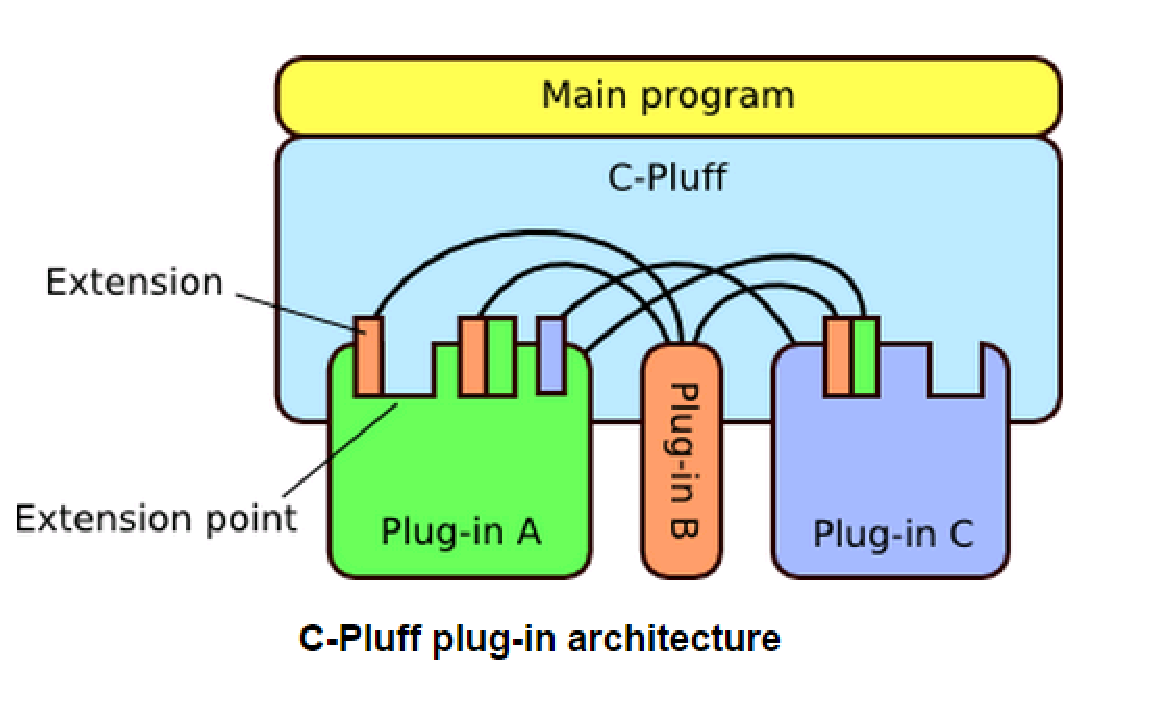
\includegraphics[height=5cm,
    angle=0]{./images/C-pluff_framework.eps}}
\caption{The main program: initialize and settup the plug-in environment.
Plug-ins integrate with each other by providing extension points and extensions.
An extension point is a point into which other plug-ins can attach extensions.}
\label{fig:C-pluff_framework}
\end{figure}

\url{http://www.c-pluff.org/reference/c-api/architecture.html}


\section{Case-study: valgrind 'core' + 'plug-ins'}


Valgrind (Sect.\ref{sec:valgrind}) is a powerful tool with 2 components:
\begin{itemize}
  \item  core: a common low-level infrastructure to support program
  instrumentation, including the JIT compiler, low-level memory manager, signal handling and a scheduler (for pthreads).
  
  The core leaves certain operations undefined, which must be filled by tools
  
  \item plug-ins: a set of tools that developed by users, and must implement
  the required list of functions for the core to use.
  
  Minimum set of functions
\begin{verbatim}
pre_clo_init()
post_clo_init()
instrument()
fini()
\end{verbatim}
\url{http://www.valgrind.org/docs/manual/writing-tools.html}
  
  The core/tool interface is not fixed. It's pretty stable these days, but it
  does change.
  
  A plug-in can also call certain functions to indicate to the core that they
  would like to use certain services, or be notified when certain interesting events
  occur. But the core takes care of all the hard work.
  
\end{itemize}

Once a plug-in is completed, it must be compiled and linked against Valgrind
core to become a complete Valgrind tool, which can be used by Valgrind via the
\verb!-tool! option to select it.

\subsection{Writing tools}


HINTS: 
From Valgrind source, the files \verb!include/pub_tool_*.h! contain all the
types, macros, functions, etc. that a tool should (hopefully) need, and are the
only .h files a tool should need to \verb!#include!.

Valgrind provides an implementation of a reasonable subset of the C library,
details of which are in \verb!pub_tool_libc*.h!



\section{Case-study: Wirebrush4SPAM}


\url{http://www.researchgate.net/profile/David_Ruano_Ordas/publication/243464849_Wirebrush4SPAM_a_novel_framework_for_improving_efficiency_on_spam_filtering_services/links/0046351d180f499daf000000.pdf}
\chapter{Macro}
\label{chap:macro}


We use \verb!#define! (Sect.\ref{sec:define}),
as discussed in Sect.\ref{sec:macro_C}.

\section{Function-like macro}
\label{sec:function-like-macro}

We put a pair of parentheses immediately after the macro name.

\begin{verbatim}
#define lang_init()  c_init()

then
     lang_init()
          ==> c_init()

but  
     lang_init
         ==> lang_init
\end{verbatim}
So,   function-like macro is only expanded if its name appears with a pair of
parentheses after it. If you write just the name, it is left alone.

\url{https://gcc.gnu.org/onlinedocs/cpp/Function-like-Macros.html}


\section{Macro that can accept any number of arguments}


Sect.\ref{sec:macro_variadic}

\section{Using \# (stringize operator, number-sign) and \#\#}


C89 standard -- that was the standard the codified the \verb!#! and \verb!##!
operators in macros and mandates recursively expanding macros in \verb!args!
before substituting them into the body if and only if the body does not apply a
\verb!#! or \verb!##! to the argument. C99 is unchanged from C89 in this
respect.

\url{http://c-faq.com/ansi/stringize.html}

\subsection{\#}

The stringize operator or number-sign operator \verb!#! is used with a
function-like macro (Sect.\ref{sec:function-like-macro}) and converts a macro
parameters into string literal immediately, without further expanding it.

\begin{verbatim}
#define make_string(x) #x
\end{verbatim}
then the parameter token immediately to the right of the \verb!#! (ignoreing
any white-spaces) is transformed by the preprocessor into a string.
Leading and trailing white space are deleted.

Application:
\begin{verbatim}
#define COMMA ,

make_string(twas brillig);
make_string( twas brillig );
make_string("twas" "brillig");
make_string(twas COMMA brillig);
\end{verbatim}
print out
\begin{verbatim}
"twas brillig"
"twas brillig"  (leading and trailing spaces from the original token are
                 removed)

"twas COMMA brillig"   (if the tokens contain another macro name, it is not
                       expaned)
\end{verbatim}

\url{http://www.complete-concrete-concise.com/programming/c/preprocessor---understanding-the-stringizing-operator}

\url{http://stackoverflow.com/questions/2751870/how-exactly-does-the-double-stringize-trick-work}

 Example:
\begin{verbatim}
#define Str(x) x
#define Xstr(x) Str(x)
#define OP plus
char *opname = Xstr(OP);
\end{verbatim}
becomes
\begin{verbatim}
char *opname = Xstr(plus) = Str(plus) = plus;
\end{verbatim}

But:
\begin{verbatim}
#define Str(x) #x
#define Xstr(x) Str(x)
#define OP plus
char *opname = Xstr(OP);
\end{verbatim}
becomes
\begin{verbatim}
char *opname = Xstr(plus) = Str(plus) = "plus";
\end{verbatim}


\subsection{\#\# (token-pasting operator, token concatenation)}

We use \verb!##! to concatenate two tokens into one token.
Here, the values (rather than the names) of two macros are to be concatenated.

This is a quite common programming trick to add a prefix or suffix to
the all the giving functions. Example
\begin{verbatim}
// deps/libncurses/include/curses.h

/*
 * Extra extension-functions, which pass a SCREEN pointer rather than using
 * a global variable SP.
 */
#if 0
#undef  NCURSES_SP_FUNCS
#define NCURSES_SP_FUNCS 20120922
#define NCURSES_SP_NAME(name) name##_sp


/* Define the sp-funcs helper function */
#define NCURSES_SP_OUTC NCURSES_SP_NAME(NCURSES_OUTC)
typedef int (*NCURSES_SP_OUTC)(SCREEN*, int);

extern NCURSES_EXPORT(SCREEN *) new_prescr (void); /* implemented:SP_FUNC */

extern NCURSES_EXPORT(int) NCURSES_SP_NAME(baudrate) (SCREEN*); /* implemented:SP_FUNC */
extern NCURSES_EXPORT(int) NCURSES_SP_NAME(beep) (SCREEN*); /* implemented:SP_FUNC */
extern NCURSES_EXPORT(bool) NCURSES_SP_NAME(can_change_color) (SCREEN*); /* implemented:SP_FUNC */
extern NCURSES_EXPORT(int) NCURSES_SP_NAME(cbreak) (SCREEN*); /* implemented:SP_FUNC */
extern NCURSES_EXPORT(int) NCURSES_SP_NAME(vidputs) (SCREEN*, chtype, NCURSES_SP_OUTC); /* implemented:SP_FUNC */

#if 1
extern NCURSES_EXPORT(char *) NCURSES_SP_NAME(keybound) (SCREEN*, int, int);	/* implemented:EXT_SP_FUNC */
extern NCURSES_EXPORT(int) NCURSES_SP_NAME(assume_default_colors) (SCREEN*, int, int);	/* implemented:EXT_SP_FUNC */
extern NCURSES_EXPORT(int) NCURSES_SP_NAME(use_legacy_coding) (SCREEN*, int);	/* implemented:EXT_SP_FUNC */
#endif

#else

#undef  NCURSES_SP_FUNCS
#define NCURSES_SP_FUNCS 0
#define NCURSES_SP_NAME(name) name
#define NCURSES_SP_OUTC NCURSES_OUTC

#endif

\end{verbatim}




\begin{verbatim}
#define COMMAND(NAME)  { #NAME, NAME ## _command }

struct command commands[] =
     {
       COMMAND (quit),
       COMMAND (help),
       ...
     };
\end{verbatim}

When a macro is expanded, the two tokens on either side of each \verb!##! operator
are combined into a single token, which then replaces the \verb!##! and the two
original tokens in the macro expansion.

Application: the first \verb!#NAME! is replaced by a string, the
second \verb!NAME ## _command! is replaced by a concatenated value (not a
string).

\begin{verbatim}
struct command commands[] = 
   }
      {"quit", quit_command},
      {"shelp", help_command}
   }
\end{verbatim}
\url{https://gcc.gnu.org/onlinedocs/cpp/Concatenation.html}
 
Example:
\begin{verbatim}
#define IIF(cond) IIF_ ## cond
#define IIF_0(t, f) f
#define IIF_1(t, f) t
\end{verbatim}

\url{https://github.com/pfultz2/Cloak/wiki/C-Preprocessor-tricks,-tips,-and-idioms}
then
\begin{verbatim}
#define A() 1
IIF(A())(true, false) 
\end{verbatim}
becomes
\begin{verbatim}
IFF_A()(true,false)
\end{verbatim}
as \verb!A()! is not expanded to 1 due to the inhibition caused by the \verb!##!
operator.

% \begin{verbatim}
% IFF_1(true,false)  
%   ==> true
% \end{verbatim}
Two-stage replacment is used
\begin{verbatim}
#define CAT(a, ...) PRIMITIVE_CAT(a, __VA_ARGS__)
#define PRIMITIVE_CAT(a, ...) a ## __VA_ARGS__
\end{verbatim}

\section{Define an a lias name}

SYNTAX: \verb!#define <new-name> <existing-name>!

\begin{itemize}
  \item for a value

\begin{verbatim}
#define true 1
#define TRUE 1
\end{verbatim}
then we can use \verb!true! or \verb!TRUE! in the code.

  \item for a type
\begin{verbatim}
#define mybyte byte;
\end{verbatim}

  \item for a function
  
\begin{verbatim}
#define sin(x) __builtin_sin(x)
\end{verbatim}

\end{itemize}

\subsection{Detect O/S}


Sect.\ref{sec:macro-detect-OS}


\section{Detect CPU}

Sect.\ref{sec:macro-detect-CPU} and Sect.\ref{sec:macro-GNU-to-detect-CPU}

\section{Detect compiler}

Sect.\ref{sec:macro-detect-compiler} and Sect.\ref{sec:macro-detect-compiler-version}


\chapter{Costs}


\section{using virtual function}
\label{sec:overhead-of-virtual-function}


Using inheritance, we can avoid the overhead of virtual functions


\section{instantiating}
\label{sec:overhead-of-instantiating}

\subsection{object in C++ vs. struct in C}
\label{sec:overhead-of-instantiating-object_in_C++-vs_struct_in_C}

In C++ the cost of instantiating an object is the same as instantiating a struct
in C.

All an object is, is a block of memory big enough to store the v-table (if it
has one - Sect.\ref{sec:V-table}) and all the data attributes. Methods consume
no further memory after the v-table has been instantiated.

\section{orders of declaration}
\label{sec:overhead-of-order-of-declaration}


\subsection{of data members}
\label{sec:overhead-of-order-of-declaration-data-members}

C++ 03 standard \verb!9/12!:
\begin{verbatim}
Nonstatic data members of a (non-union) class declared without an intervening
access-specifier are allocated so that later members have higher addresses 
within a class object. 
The order of allocation of nonstatic data members separated 
by an access-specifier is unspecified (11.1). 
Implementation alignment requirements might cause 
two adjacent members not to be allocated immediately after each other; 
so might requirements for space for managing virtual functions (10.3) 
and virtual base classes (10.1).
\end{verbatim}
\url{http://stackoverflow.com/questions/3824213/does-order-of-members-of-objects-of-a-class-have-any-impact-on-performance}

\subsection{of objects}
\label{sec:overhead-of-order-of-declaration-objects-in-a-function}


C++ guarantees that the order of objects in memory is the same as the order of
declaration, unless an access qualifier intervenes.

Objects which are directly adjacent are more likely to be on the same cacheline,
so one memory access will fetch them both (or flush both from the cache). Cache
effectiveness may also be improved as the proportion of useful data inside it
may be higher. Simply put, spatial locality in your code translates to spatial
locality for performance.


Order may affect the amount of padding.  Unnecessary padding may increase the
total size of the structure, leading to higher memory traffic.
\url{http://stackoverflow.com/questions/3824213/does-order-of-members-of-objects-of-a-class-have-any-impact-on-performance}




\part{I/O}
\chapter{Pseudo-random number generators}


A true random number sequence is a sequence that has no repetition,
i.e. the cycle is infinity. Indeed, you can never have a true random
number generator. However, when the cycle (period length) is big
enough, it is statistically indistinguishable from a true random
sequence. So, such sequences is called a {\it pseudorandom} (or
quasi-random) number sequence. The generator is called pseudo-random
number
generator\footnote{\url{http://infohost.nmt.edu/tcc/help/lang/fortran/random.html}}.

Each generator need one initial value or a sequence of values called
the {\it seed} numbers. With a given seed number, the generator will
produce a unique sequence of pseudorandom values.
\textcolor{red}{Two sequences from the same seed number(s) are the
  same; thus is convenient for debugging purpose or performance
  comparisons}.

Labs doing research on RGN:
\begin{itemize}
\item \url{http://random.mat.sbg.ac.at/}: Univ. of Salzburg
\end{itemize}

While a long period is not a guarantee of quality in a random number generator,
short periods (such as the $2^{32}$ common in many older software packages) can be
problematic. 

At the lowest level, the solution of generating random numbers is the solution
that generate bits (0 and 1) at different positions of the $k$-bit words at the
same likelihood (for uniform distribution). This is the role of the {\bf engine} (term used in C++11).
\textcolor{red}{From the sequence of uniform distribution, we can generate the sequence of any other distribution.}
This is the role of the {\bf distribution} component.



\section{Mersene Twistter}
\label{sec:PRNG_Mersenne-Tiwstter}

{\bf Mersenne Twister} (developed 1997 by Matsumoto and Nishimura) is the most widely used PRNG methods.
It is the default PRNG for many programming languages (R, Python, IDL, MatLab, MS Visual C++)

It was the first to provide (1) fast generation of high-quality PRNs, i.e. overcome most of the flaws found in older PRNGs.

The sequence is based on the Mersenne prime, a prime number in the form $M_n =
2^n-1$, i.e. a prime number which is one less than a power of two.
\url{http://en.wikipedia.org/wiki/Mersenne_prime}

The commonly used version is 
\begin{itemize}
  \item MT19937: use 32-bit word length with very long sequence of $n=19937$
  
  \item MT19937-64: use 64-bit word length, and generate a different sequence.
\end{itemize}

For many applications, the state space $2^{252}-1$ is enough.
In 2011, Saito \& Matsumoto proposed a version of the Mersenne Twister to
address this issue. The tiny version, TinyMT, uses just 127 bits of state space.

The seed is a $k$-bit word length, which is then used to generate integers in the range $[0, 2^k-2]$.


\subsection{SFMT, dSFMT}
\label{sec:sfmt}
\label{sec:dSFMTs}

SFMT, the Single instruction, multiple data-oriented Fast Mersenne Twister, is a
variant of Mersenne Twister, introduced in 2006, designed to be fast when it
runs on 128-bit SIMD. Intel SSE2 and PowerPC AltiVec are supported by SFMT.

SFMT stands for SIMD-oriented Fast Mersenne Twister. SFMT generates
single-precision data. For double precision, it has dSFMT.
dSFMT only works on CPUs which use IEEE 754 format double precision
floating point numbers.

The current version of SFMT (1.3.3) supports the periods from
$2^{607}-1$ to $2^{216091}-1$.

The current version of dSFMT (2.1) supports the periods from
$2^{521}-1$ to $2^{216091}-1$.

References:
\begin{itemize}
\item
  \url{http://www.math.sci.hiroshima-u.ac.jp/~m-mat/MT/SFMT/index.html}
\item \url{http://www.math.sci.hiroshima-u.ac.jp/~m-mat/MT/emt.html}
\item \url{http://www.codeproject.com/KB/DLL/SFMT_dll.aspx}
\end{itemize}



\subsection{MTGP}
\label{sec:mtgp}

MTGP is a variant of Mersenne Twister optimised for graphics processing units (GPU)
published by Mutsuo Saito and Makoto Matsumoto.

MTGP stands for Mersenne Twister for GPU Processor that supports both
32-bit and 64-bit (1) unsigned integer and (2) floating point numbers
based on IEEE 754 formats. Thus, we have totally 2 set of files,
representing by their prefixes: \verb!mtgp32-! and \verb!mtgp64-!.
For each version, correspondingly, there are two different
implementations:
\begin{itemize}
\item simple version: representing by their suffixes, \verb!-ref.c!
\item fast version : representing by their suffixes, \verb!-fast.c!
\begin{verbatim}
mtgp32-fast.h               mtgp64-fast.h
mtgp32-fast.c               mtgp64-fast.c
mtgp32-param-fast.c         mtgp64-param-fast.c
\end{verbatim}
\end{itemize}

MTGP can generate uniformly distributed pseudo-random sequences of
some given periodic length \verb!mexp!, e.g. ${23209}, {11213}$...
\begin{itemize}
\item 64-bit RNG has periods of either $2^{23209}-1$, $2^{44497}-1$
  and $2^{110503}-1$.
\item 32-bit RNG has periods of either $2^{11213}-1$, $2^{23209}-1$
  and $2^{44497}-1$.
\end{itemize}
Each version support some predefined set of seed values for some given
periods \verb!mexp!. In version 1.0.2, each period has total 128
different sets of seed values, each set will help generate one random
sequence. All sets of seed data are stored in two files: one for the
simple version (\verb!mtgp64-param-ref.c!), one for the fast version
(\verb!mtgp64-param-fast.c!).

\begin{framed}
  If you want more parameter set, i.e. more random sequences, you need
  to use MTGP Dynamic Creator (MTGPDC) which can create $2^{32}$
  parameter sets for the following periods $2^{3217}, 2^{4423},
  2^{11213}, 2^{23209}, 2^{44497}$ (ver. 1.0.2). Download the source
  code from the same website.
\end{framed}

We will discuss how to work with the ``fast'' 64-bit version using one
of the 128 given parameter sets for seeding.  The file
\verb!mtgp64-param-fast.c! contains three arrays
\begin{verbatim}
mtgp64_params_fast_23209
mtgp64_params_fast_44497
mtgp64_params_fast_110503
\end{verbatim}
of the derived type \verb!mtgp64_params_fast_t!.

\begin{framed}
  The code only works on systems that support IEEE 754 floating-point
  format. Its, however, run very slow on CPU; and fast on GPU.
\end{framed}

What we need to do
\begin{enumerate}
\item \verb!params! point to the correct structure element in one of
  the three above arrays (given via \verb!mexp! and \verb!no! values)
\begin{lstlisting}
mtgp64_params_fast_t * params;

int mexp; // periods, either 44497, 23209 or 110503
          //+ for double precision
int no;   // should be within 0 to 127

read_in(&mexp, &no);

switch (mexp) {
case 44497:
  params = mtgp64_params_fast_44497;
  break;
case 23209:
  params = mtgp64_params_fast_23209;
  break;
case 110503:
  ...
default:
  ...
}

if (no >= 128 || no < 0) {
  printf("error");
}
\end{lstlisting}

\item initialize internal state
  \begin{itemize}
  \item (CPU version) given by the variable \verb!mtgp64!
  \begin{itemize}
  \item  \verb!mtgp64-init! allocates and init the
    internal state (first argument) given \verb!params! (2nd argument)
    and a single integer seed (third argument)
  \item  \verb!mtgp64_init_by_array! .... and an array of
    seed values (3rd argument, with length information is the 4th
    argument)
  \item  \verb!mtgp64_init_by_str! .... and the string is
    terminated by zero (3rd argument)
  \end{itemize}
\begin{lstlisting}
mtgp64_fast_t mtgp64;

/* Seed value */
/* --> scalar or an array or a string array */
uint64_t seed = 1;
uint64_t seed_ar[4] = {1, 2, 3, 4};
char seed_str[] = "\01\02\03\04";

params += no;
rc = mtgp64_init(&mtgp64, params, seed);

rc = mtgp64_init_by_array(&mtgp64, params, seed_ar, 4);
\end{lstlisting}

\item (GPU version)  (\verb!d_status)!
  \begin{itemize}
  \item  \verb!mtgp64_init_state! allocates and init the
    internal state (first argument of type \verb!uint_64!) given
    \verb!params! (2nd argument) and a single integer seed (third
    argument). This function is called internally by
    \verb!make_kernel_data!
  \item \verb!make_kernel_data (d_status, params)!
  \end{itemize}
\begin{lstlisting}
#define MEXP 23209
#define LARGE_SIZE (THREAD_NUM*3)
#define BLOCK_NUM_MAX 200
#define TBL_SIZE 16

mtgp64_kernel_status_t * d_status;

int block_num;
int block_num_max;

\end{lstlisting}
\end{itemize}


\item  generate random data
  \begin{itemize}
  \item (CPU version) (given the internal state \verb!mtgp64!)
  \begin{itemize}
  \item \verb!mtgp64_genrand_uint64(mtgp64)! : generate a 64-bit
    single 64-bit unsigned integer.
  \item \verb!mtgp64_genrand_close1_open2! : generate a
    double-precision pseudo-uniformly distributed in the range [1,2]
  \item \verb!mtgp64_genrand_close_open! : generate a double-precision
    pseudo-random uniformly distributed in the range $[0,1)$
  \item \verb!mtgp64_genrand_open_close! : generate a double-precision
    pseudo-random uniformly distributed in the range (0,1]
  \item \verb!mtgp64_genrand_open_open! : generate a double-precision
    pseudo-random uniformly distributed in the range (0,1)
  \end{itemize}

\begin{lstlisting}
/* Generate 100 random values */
for (i=0; i< 100; i++) 
   rnd_value[i] = mtgp64_genrand_uint64(mtgp64);
\end{lstlisting}

\item (GPU version) generate random data (given the internal state
  \verb!d_status!)
  \begin{itemize}
  \item \verb!mtgp64_uint64_kernel(mtgp64_kernel_status *d_status!,
    \verb!uint64_t* data, int size)!: generate an array of 64-bit
    unsigned integer.
  \item \verb!mtgp64_double_kernel(d_status, *d_data, int size)!:
    generate an array of double precision floating point numbers in
    \verb!d_data!. 
  \item \verb!make_constant(const params[], int block_num)!: set
    constants in device memory
  \item \verb!make_texture(const params[], *d_texture_tbl[3],!  int
    \verb!block_num)!: set constants in device memory

  \item CALL FROM HOST: \verb!make_uint64_random(*d_status!, int
    \verb!num_data, int block_num)! - generate 64-bit unsigned random
    numbers, \verb!make_double_random(*d_status, int num_data!,
    \verb!int block_num)!  - generate double precision random numbers
  \end{itemize}
\end{itemize}
\end{enumerate}

\subsubsection{Sample codes}
\label{sec:sample-codes}

In the folder \verb!/cuda_sample!, there are some files
\begin{itemize}
\item \verb!mtgp32-*!: for 32-bit
\item \verb!mtgp64-*!: for 64-bit
  \begin{itemize}
  \item \verb!mtgp64-cuda13-tex.cu!: CUDA 2.3, with texture and SM1.3
    (support double precision)
  \item \verb!mtgp64-cuda-tex.cu!: CUDA 2.3, with texture and
    single-precision only
  \item \verb!mtgp64-cuda.cu!: CUDA 2.2
  \item \verb!mtgp64-cuda-common.c!: to be included by the above files
  \end{itemize}
\end{itemize}


References:
\begin{itemize}
\item \url{http://www.math.sci.hiroshima-u.ac.jp/~m-mat/MT/MTGP/index.html}
\end{itemize}

\section{Libraries}

CUDA:
\begin{itemize}
  \item CURAND: pseudo-random number generators
  \item SARU: Sect.\ref{sec:saru}
\end{itemize}


\section{Generate data in parallel}
\label{sec:gener-data-parall}

\subsection{CUDA Sample MersenneTwister}
\label{sec:cuda-mersennetwister}

CUDA C has a sample implemented the MersenneTwister with cycle
$2^{607}-1$. Each twister is run for each thread

\subsection{SPRNG}
\label{sec:sprng}

SPRNG stands for Scalable Parallel Number Generator. It use MPI for
parallel data generator.

References:
\begin{itemize}
\item \url{http://sprng.cs.fsu.edu/}
\end{itemize}


\subsection{SARU}
\label{sec:saru}

SARU is a 32-bit PRNG that can provide a single-precision or
double-precision uniform distributed random number in the range
$[0,1)$. This base PRNG can be used to generate many other
distributions. 

SARU was developed by Steve Worley. 
%%
%% GenerateData.tex
%% Login : <hoang-trong@hoang-trong-laptop>
%% Started on  Thu Oct  1 12:07:44 2009 Hoang-Trong Minh Tuan
%% $Id$
%% 
%% Copyright (C) 2009 Hoang-Trong Minh Tuan
%%

\chapter{Generate Data}
\label{chap:generate-data}

The Mersenne Twister algorithm (Sect.\ref{sec:PRNG_Mersenne-Tiwstter}) is
available in C++ language since C++11 standard.

In early version of C++, the header file \verb!cstdlib! (C++) or \verb!stdlib.h! provides function for PRNGs
\begin{itemize}
  \item \verb!RAND_MAX! - a macro that extends to an integer constant
  
  \item \verb!std::rand()! - a function returning a PRN in the interval \verb!(0, RAND_MAX)!
  
  \item \verb!std:srand()! - pass a seed to the PRNG used by \verb!std:rand()!
\end{itemize}
The algorithms underlying even this minimal support have typically been unspecified, and
hence their use has historically been nonportable. 
\url{http://www.open-std.org/jtc1/sc22/wg21/docs/papers/2013/n3551.pdf}

\section{C++11: <random>}
\label{sec:C++11_random}


C++11 provides a new header file for PRNG 
\begin{lstlisting}
#include <random>
\end{lstlisting}
In C++11, there is a clear difference between the {\bf engine} and the {\bf distribution}.
\begin{itemize}
  \item the {\bf engine}'s role is to return unpredictable (random) bits, ensuring the probability (or likelihood) of obtaining
  a 0 bit is always the same as that of obtaining a 1 bit.
  
The purpose of the engine is to serve as a source of randomness. The sequence would be in uniform distribution.  
  
  \item the {\bf distribution}'s role is to convert the bits in uniformly distributed sequence into the number of proper distribution.
\end{itemize}
The terms engine and distribution are applied not only to types meeting certain requirements specified in the C++11
standard, but also to objects of such types.

\subsection{Create an engine}

The engine controls the sequence of PRNG.
The two engines initialized of the same state always return the same two sequence of PRNGs.
Such replication can be very useful while debugging a program or reproducing research, for example.

To escape replication, the engine's seed must vary from run to run
\begin{itemize}
  \item traditional approach: use system clock, \verb!time(0)!, or access to system-specific resource, \verb!/dev/urandom!
  
  \item C++11 approach: use \verb!std::random_device! as the seed
\end{itemize}

There are two ways to initialize an engine: implicit vs. explicit (which we can
also provide a seed). The type of the seed must be the same as (or convertible
to) the type of the values produced by the engine.


\begin{verbatim}
#include <random>

std::default_random_engine e1; // implicitly default-initialized
static std::default_random_engine e{};  // explicit default-initialized

std::default_random_engine e3{13607};

std::random_device rdev{};
std::default_random_engine e{rdev()};
\end{verbatim}

An engine's state can be reset any time after it has been initialized
\begin{lstlisting}
void f( std::default_random_engine & e4, std::random_device & rd )
{
  e4.seed(13607); // e4 state now as if initialized by 13607

  e4.seed(); // now as if default-initialized

  e4.seed(rd()); // now as if initialized via the device-obtained seed
}
\end{lstlisting}

List of all engines:
\begin{itemize}
  \item light-weight use:   \verb!std::default_random_engine!
  \item knowledge use: 
\begin{itemize}
  
  \item \verb!std::mt19937!, \verb!std::mt19947_64!: mersenne twister
  
  \item \verb!minstd_rand0, minstd_rand!: linear congruential engines
  
  \item \verb!ranlux24_base, ranlux48_base!: subtract with carry engine
  
   \item \verb!ranlux24, ranlux48!: discard block engine
   \item \verb!knuth_b! : shuffle order engine
\end{itemize}
  \item for expert (researcher): the following templates can be configured via template parameters 

\begin{verbatim}
linear_congruential_engine 
discard_block_engine
mersenne_twister_engine 
independent_bits_engine
subtract_with_carry_engine 
shuffle_order_engine

\end{verbatim}
\end{itemize}

\subsection{Create a distribution}

{\bf Uniform distribution}:
\begin{lstlisting}
int lbound = 1;
int ubound = 6;
static std::uniform_int_distribution<int> d{lbound, ubound};
\end{lstlisting}

\url{http://www.open-std.org/jtc1/sc22/wg21/docs/papers/2013/n3551.pdf}

\subsection{Return a PRN based on the created distribution and engine}

We pass the engine to the distribution.

\begin{lstlisting}
#include <random>
int roll_a_fair_die( )
{
  static std::default_random_engine e{};
  static std::uniform_int_distribution<int> d{1, 6};
  return d(e);
}
\end{lstlisting}




\section{File with given sizes}

Create file at a given size, containing only zeros
\begin{verbatim}
dd if=/dev/zero bs=1024 count=<number-of-kilobytes> > myfile
\end{verbatim}

%%% Local Variables: 
%%% mode: latex
%%% TeX-master: "fortran_manual"
%%% End: 

\chapter{Command-line arguments}
\label{chap:command-line-argument}

\section{History}

Unix tradition encourages the use of command-line switches to control programs, so that options can be specified from scripts.
We can pass the input via the command-line arguments
\begin{verbatim}
python <source.py>  arg1 arg2
\end{verbatim}
\url{http://www.faqs.org/docs/artu/ch10s05.html}

A program can accepts commands (tcp, serial), and keyword arguments
\begin{verbatim}
my_prog tcp <host> <port>  [--timeout=<second>]
my_prog serial <port> [--baud=9600] [--timeout=<second>]
my_prog (-h | --help | --version)
\end{verbatim}
A command can accepts as a series of positional arguments (\verb!<host>, <host>!) 
and/or keyword arguments (\verb!--timeout=<second>!).


There are 3 types of command-line arguments:
\begin{itemize}
  \item positional argument
  \item optional argument
  \item keyword argument (named argument)
  \item flags
\end{itemize}

\begin{mdframed}

David Goodger pointed out that the term \verb!keyword argument! - on Unix
platforms - traditionally called \verb!options!;  what he calls \verb!values!
are traditionally called \verb!option arguments!; and what he calls
\verb!positional arguments!, the Open Group calls \verb!operands!.
\begin{itemize}
  \item First of all, the term option tends to be Unix-specific; on Windows the term parameter is more frequently used
  \item Second, the investigation began with command-line parsers, and in the context of a discussion of parsers and parsing, keyword argument seems a more traditional and appropriate term than option. 
  \item Third, the usual definition of option is not very useful.
  \item And finally, the term option implies optionality.  Whether an argument is optional or required is a semantic issue rather than a syntactical issue. 
\end{itemize}

\end{mdframed}

\url{https://pythonconquerstheuniverse.wordpress.com/2010/07/25/command-line-syntax-some-basic-concepts/}


\subsection{-- positional argument}
\label{sec:positional-argument}

{\bf positional arguments}: a bare value and its position in a list of
  arguments identifies it.
\begin{verbatim}
rename file_a.txt  file_b.txt
\end{verbatim}  
The order is important in positional arguments.

\subsection{-- optional argument}
\label{sec:optional-argument}

({\bf optional argument}) or the term \verb!keyword argument! is used to
  cover both {\bf named arguments} and {\bf flags}.
  
A \verb!keyword argument! requires a sigil (a special character of string of
characters that indicates the beginning of a key).

\begin{itemize}
  \item In Windows, a sigil is a forward slash (/)
  \item In Unix-like O/S, a sigil is a dash (-) for single-character name, and
  two dash (\verb!--!) for longer name

Some applications, especially on Unix, make a distinction between
single-character keys and multi-character keys ("long options"), with a
single-dash sigil "-" indicating the beginning of a single-character key, and a
double dash "\verb!--!" sigil indicating the beginning of a multi-character key.

  \item Some applications use multiple sigils.  With the plus sign '+' as a
  sigil, for instance, it is possible to use flags to turn options on and off.
    
   \item EXCEPTION: some programs do not use sigil in front of the optional
   argument

\begin{verbatim}
tar xvf <filename.tar>
\end{verbatim}
This is not recommended.
   
   \item  Some programs allow several single-letter options to be preceded by a
   single dash e.g. "ps -elf" instead of "ps -e -l -f". 
   
   This is also not recommended.
   \url{http://courses.cms.caltech.edu/cs11/material/c/mike/misc/cmdline_args.html}
\end{itemize}

\subsection{-- named argument}
\label{sec:named-argument}
{\bf named arguments}: a (keyword, value) pair, where the key
  identifiers the value
  
  It is  identified by placing a dash (-) before the optional argument's name
\begin{verbatim}
my_prog -a value
my_prog -a=value

my_prog --afullname value
my_prog --afullname=value
\end{verbatim}  
% 

A \verb!named argument! needs a mechanism to separate keys from argument values
\begin{itemize}
  \item use whitespace 
\begin{verbatim}
rename  -o file_a.txt  -n file_b.txt
\end{verbatim}  

  \item use equal sign (=) in Unix, and colon (:) in Windows
\begin{verbatim}
 # Unix
rename  -o=file_a.txt  -n=file_b.txt
 # Windows
rename  /o:file_a.txt  /n:file_b.txt
\end{verbatim}

  \item use the known-length (1-character)
  
\begin{verbatim}
rename  -ofile_a.txt  -nfile_b.txt
\end{verbatim}
\end{itemize}

Several fixed-length \verb!flags! can be concatenated
\begin{verbatim}
tar -x -v -f  some_filename.tar

tar -xvf some_filename.tar
\end{verbatim}
NOTE: "--xvf" (note the double dash) indicates a single multi-character flag: "xvf".

\subsection{-- flags}
\label{sec:flags-in-argument}

{\bf flags}: a stand-alone keyword, whose presence or absence provides
  information to the application
\begin{verbatim}
my_prog -a -b

my_prog --afullanme --bfullname
\end{verbatim}  

Although it is possible to think of flags as degenerate named arguments (named
arguments that have a key but no value), it is easier to think of flags as a
distinct type of argument, different from named arguments.


\section{Parsing command-line arguments}

We need to loop through the number of argument \verb!argc!, including the name
of the excutable file as the 0-th argument. 

\subsection{Simple}


{\small 
\begin{verbatim}
// When passing char arrays as parameters they must be pointers
int main(int argc, char* argv[]) {
    if (argc < 5) { // Check the value of argc. If not enough parameters have been passed, inform user and exit.
        //print help
        std::cerr << "Usage is -in <infile> -out <outdir>\n"; 
        std::cin.get();
        exit(0);
    } else { // if we got enough parameters...
        char* myFile, myPath, myOutPath;
        std::cout << argv[0];
        for (int i = 1; i < argc; i++) { /* We will iterate over argv[] to get the parameters stored inside.
                                          * Note that we're starting on 1 because we don't need to know the 
                                          * path of the program, which is stored in argv[0] */
            if (i + 1 != argc) // Check that we haven't finished parsing already
                if (argv[i] == "-f") {
                    // We know the next argument *should* be the filename:
                    myFile = argv[i + 1];
                } else if (argv[i] == "-p") {
                    myPath = argv[i + 1];
                } else if (argv[i] == "-o") {
                    myOutPath = argv[i + 1];
                } else {
                    std::cout << "Not enough or invalid arguments, please try again.\n";
                    Sleep(2000); 
                    exit(0);
            }
            std::cout << argv[i] << " ";
        }
        //... some more code
        std::cin.get();
        return 0;
    }
}
\end{verbatim}
}

\subsection{Using std::string::find()}

\begin{lstlisting}
#include <algorithm>

char* getCmdOption(char ** begin, char ** end, const std::string & option)
{
    char ** itr = std::find(begin, end, option);
    if (itr != end && ++itr != end)
    {
        return *itr;
    }
    return 0;
}

bool cmdOptionExists(char** begin, char** end, const std::string& option)
{
    return std::find(begin, end, option) != end;
}

int main(int argc, char * argv[])
{
    if(cmdOptionExists(argv, argv+argc, "-h"))
    {
        // Do stuff
    }

    char * filename = getCmdOption(argv, argv + argc, "-f");

    if (filename)
    {
        // Do interesting things
        // ...
    }

    return 0;
}
\end{lstlisting}
\url{http://stackoverflow.com/questions/865668/parse-command-line-arguments}

\subsection{Using GetOpt class - C++}

You can use GNU GetOpt (LGPL) or one of the various C++ ports, such as getoptpp
(GPL).

\url{http://www.chemie.fu-berlin.de/chemnet/use/info/libgpp/libgpp_39.html}

\subsection{Using getopt() - C language}
\label{sec:getopt()}

Here, we use \verb!getopt()! and \verb!optarg! variable. IMPORTANT: We need to
end the list of argument with semicolon (:)
\begin{verbatim}
#include <getopt.h>

std::string val1;
int val2;

//ERROR:you will get std::logic_error
//while ((c = getopt(argc,argv,"i:v:e:f")) != -1)

//CORRECT
while ((c = getopt(argc,argv,"i:v:e:f:")) != -1)
{
  switch(c) {
  case 'i':
  	val1 = optarg;
	break;
  case 'v':
    val2 = atoi(optarg);
    break;
  case 'e':
  	break;
  case 'f':
    break;
    
   default: /* '?' */
            fprintf(stderr, "Usage: %s [-t nsecs] [-n] name\n",
                    argv[0]);
            exit(EXIT_FAILURE);
 }
}
\end{verbatim}

\subsection{OptionParser}

\url{http://stackoverflow.com/questions/865668/parse-command-line-arguments}

\url{http://sourceforge.net/projects/optionparser/}

\subsection{CLPP: C++ Command-line parser (use Boost)}

\url{http://sourceforge.net/projects/clp-parser/}

\subsection{Using Boost.Program\_Options}

{\small \begin{verbatim}
#include <boost/program_options.hpp>
namespace po = boost::program_options;

int main(int argc, char** argv){
  try{
    int opt;
    po::options_description desc(``Allowed options'');
    desc.add_options() // list all options
       (``help,h'', ``produce help message''),

       //the second part after ',' is short, i.e. --file or -f
       (``file,f'', po::value<std::string>(), ``the file to read in''),
       (``task'', po::value<std::vector<int> >(), ``accept multiple values'')

       //we can set default value here (10) and the address (&opt) to store the
       //value
       // so if user don't pass the argument, it use 10 
       ("optimization", po::value<int>(&opt)->default_value(10), 
          "optimization level")

       //so if user pass the argument with no value, it use 10
       //, e.g. ./a.out --width   #use 10
       //       ./a.out --witdh=80 # use 80
       //NOTE: for short option, the value must be immediately after the option
       //./a.out -w80   # implicit_value not used
       //./a.out -w 80  # wrong: 80 parsed as extra arg if implicit_value is
       //               defined 
      ("witdh,w", po::value<int>(&opt)->implicit_value(10), 
          "width")

       //it can accept multiple values
       //or use the option several times
       //either way, the result will be a vector
       ("include-path,I", po::value< vector<string> >(), 
             "include path")
       ("input-file", po::value< vector<string> >(), "input file")
       
       // you don't want a vector but a single value and that 
       // a single value can span multiple tokens
       // e.g. --email beadle@mars beadle2@mars
       ("email", value<string>()->multitoken(), "email to send to")
       
       // we can add semantic
       // which need to use boost::program_options::value_semantic class
       ("email", value< vector<string> >()
        ->composing()->notifier(&your_function), "email")          
    ;	
    
    po::variables_map vm; //store values of options (of arbitrary types)
    po::store(po::parse_command_line(argc, argv, desc), vm);
    po::notify(vm);
  
    if (argc == 1 || vm.cout(``help'')){
       std::cout << desc << ``\n'';
       return 0;
    }

//IMPORTANT: Once you use address (e.g. &opt)
// you don't have to use if for getting option's value    
    if (vm.cout(``file'')) //check the using of one argument option
    {
       myfile = std::string(vm[``part''].as<std::string>());
    }
    if (vm.cout(``type'')) //integer
    {
       mytype = vm[``type''].as<int>();
    }
    if (vm.cout(``task'')) //multiple values
    {
      std::vector<int> list_task = vm[``task''].as< std::vector<int> >();
      //loop
      for (std::vector<int>::iterator iter=list_task.begin(); iter <
          list_task.end(); iter++) {
          //do something
      } 
    }
  }catch (std::exception &e){
    std::cerr << ``error: `` << e.what() << ``\n'';
    return 1;
  }catch (...){
    std::cerr << ``Exception unknown type \n'';
  }
}
\end{verbatim}}

There are case that we want the option-name to be hidden, e.g.
\begin{verbatim}
compiler a.cpp
compiler --input-file=a.cpp
\end{verbatim}
then we need to tell \verb!input-file! is the ``positional options''
\begin{verbatim}
po::positional_options_description p;
p.add("input-file", -1); // (name, how-many-positional-options)
   // value=1 : exactly one, first, positional option is assigned to input-file
   // value=2 : the first two positional option is assigned to input-file
   // value=-1: any others 
  // all positional options should be translated into 
  // values for 'input-file' option

po::variables_map vm;
  //and we use different function
  // command_line_parser(...)
po::store(po::command_line_parser(ac, av).
          options(desc).positional(p).run(), vm);
po::notify(vm);
\end{verbatim}

Now you want to have options organized into different groups: some are read from
the config file, so that frequently used options can be passed easily, or we
split options into different groups (some can only be used  in the config file,
some should be hidden from user, etc.), we then use more complicated approach
like the following. NOTE: 
The value passed to the command line should override the value from the config file.
\begin{verbatim}
// Declare a group of options that will be 
// allowed only on command line
po::options_description generic("Generic options");
generic.add_options()
    ("version,v", "print version string")
    ("help", "produce help message")    
    ;
    
// Declare a group of options that will be 
// allowed both on command line and in
// config file
po::options_description config("Configuration");
config.add_options()
    ("optimization", po::value<int>(&opt)->default_value(10), 
          "optimization level")
    ("include-path,I", 
         po::value< vector<string> >()->composing(), 
         "include path")
    ;

// Hidden options, will be allowed both on command line and
// in config file, but will not be shown to the user.
po::options_description hidden("Hidden options");
hidden.add_options()
    ("input-file", po::value< vector<string> >(), "input file")
    ;     
\end{verbatim}

then we put them into groups we want
\begin{verbatim}
po::options_description cmdline_options;
cmdline_options.add(generic).add(config).add(hidden);

po::options_description config_file_options;
config_file_options.add(config).add(hidden);

po::options_description visible("Allowed options");
visible.add(generic).add(config);
\end{verbatim}


\url{http://www.boost.org/doc/libs/1_54_0/doc/html/program_options/overview.html}

% \section{File locking}
% \label{sec:file-locking}

\subsection{Using popt library}
\label{sec:popt_lib}

The popt library exists essentially for parsing command line options. Some
specific advantages of popt are no global variables (allowing multiple passes in
parsing argv), parsing an arbitrary array of argv-style elements (allowing
parsing of command-line-strings from any source), a standard method of option
aliasing, ability to exec external option filters, and automatic generation of
help and usage messages.    

\url{http://directory.fsf.org/wiki/Popt}

\subsection{TCLAP}
\label{sec:TCLAP}

\url{http://tclap.sourceforge.net/}


\chapter{I/O}
\label{chap:IO}

It is important to understand that the data saved in the file can be in binary
format or human-readable format. With human-readable format, it can be in any
external representation (ASCII, Unicode, \ldots).

 
\section{Encoding schemes}
\label{sec:character_sets}
\label{sec:encoding-scheme}

\begin{itemize}

  \item A {\bf character set} is a collection of graphic characters, which are
  symbols such as letters, numbers, and punctuation marks. 
  
  \item A {\bf set of code points} is a set of hexadecimal values (binary values
  stored in the computer). 
  
  Depending how many characters in a character set, the computer needs to use
  one byte or more to store the code points. With a character set of no more
  than 255 characters, then only 1-byte is needed.
  
  If only 1-byte is used, then it's quite simple. However, if there are more
  than one byte is used, then the order between the bytes to represent one code
  point should be considered. This makes the comparision between characters or
  strings or reading/writing the string data complicated.

  \item  An {\bf encoding schemes} specify how to map each character in a
  character sets to each haxadecimal value in a set of code points.

Examples of encoding schemes: EBCDIC, (7-bit) ASCII, 8-bit ASCII, Windows-1252,
Unicode, ISO 10646.

\end{itemize}

\subsection{Single-byte encoding scheme: ANSI (ANSI\_X3.4-1968 (ISO/IEC
646-1972), ISO/IEC 8859 Latin 1), Windows-1252}
\label{sec:ANSI}

ASCII (ANSI\_X3.4-1968, ISO/IEC 646-1972) is a character-encoding scheme for 128
specified characters \footnote{\url{http://en.wikipedia.org/wiki/ASCII}}. ASCII
character requires only 7-bit for storing code points. 

The ASCII extension (ANSI 8-bit) allows more characters to be added in. 
The first standard for ASCII 8-bit is ISO/IEC 8859 Latin 1 (or simply ISO Latin
1), with characters in the range 128-255 to represent Latin character. Another
popular encoding scheme representing 8-bit character set by Microsoft was
Windows-1252.

IBM PC defined {\it code page 437}, which define the graphical representation
for ASCII characters and some special European characters on the screen. 

\subsection{Multiple-byte encoding scheme: Unicode, ISO 10646}

To deal with more characters (internationalization), newer standards were
developed. MSE (multibyte support extension) was designed to describe
specification on how to add extended character sets to C language. If more than
one byte is required to store code points for characters, then the character set
is called a wide-character set.
Before 1991, the two widely used wide-character sets were Unicode
and ISO 10646 (defined by UCS - Universal Character Set).

The first draft of Unicode was published in 1988 by Joseph D.
Becker.\footnote{\url{http://www.utf8everywhere.org/}} At that time, he believed
16-bit was enough, with the higher byte set to 0 and the lower byte represents
ISO Latin 1 characters.
\footnote{\url{http://www.codeguru.com/cpp/misc/misc/multi-lingualsupport/article.php/c10451/The-Basics-of-UTF8.htm}}
Initially, UNICODE offers support for alphabets from Europe, Africa, Middle
East, Asia (including the unified Han set of East Asian ideograms and the
complete ideograms for Korean Hangul).

\textcolor{red}{Unicode was first designed for 16-bit; while ISO 10646 uses
31-bit}.

From 1991, ISO Working Group and Unicode consortium have coordinated to work on
a single universal standard for multilingual
text.\footnote{\url{http://www.unicode.org/faq/unicode_iso.html}}. However, they
are not exactly the same, as Unicode standard imposes some additional
constraints to make sure cross-platform and applications compatible,
bidirectional algorithms for right-to-left scripts, etc.
\textcolor{red}{Nowadays, Unicode is the widely accepted encoding scheme for
characters}.

Here is the information which Unicode version matches with ISO 10646 version.
\begin{itemize}
  \item Unicode 2.0 (1993): ISO/IEC 10646-1:1993 plus Amendment 5 to 7
  \item Unicode 3.0 (2000): ISO/IEC 10646-1:2000. 
  
The first 65,536 (the Basic Multilingual Plane, or BMP) had entered into common
use before 2000.  Since 2000, China requires all software sold in their country
must support GB 18030, i.e. moving beyond BMP.
    
  \item Unicode 4.0 (2003): ISO/IEC 10646:2003 
  
  \item Unicode 5.0 (2003): ISO/IEC 10646:2003 add Devanagari Letters GGA, JJA,
  DDDA and BBA
  
  \item Unicode 6.0 (2011): ISO/IEC 10646:2011 add Indian Rupee Sign
  \item Unicode 6.1 (2012): ISO/IEC 10646:2012
  \item Unicode 6.2 (2012): ISO/IEC 10646:2012 add Turkish Lira Sign
\end{itemize}

\subsection{Multiple-byte length-variant encoding scheme: UTF-7,
UTF-7.5, UTF-8, UTF-16, UTF-32}

In Unicode:The first 0x10000 code positions is called Basic Multilingual Plane
(BMP). For maximum compatibility, individual Unicode characters are passed
around using 32-bit integer (4-byte per character). However, storing 4-byte per
character is wasteful most of the time.

To improve space saving, different intermediate encoding schemes (Universal
Transformation Format) have been developed (UTF-7, UTF-7.5, UTF-8, UTF-16,
UTF-32). 

UTF-8 is currently the most widely used encode (as the small resulting size of
the string), e.g. filenames in Linux and is supported by all mainstream
webbrowsers. 

\subsection{UTF-8}

The information for UTF-8 is given below.

\begin{verbatim}
   UNICODE            |     UTF-8 (bits representation)
00000000 -- 0000007F: 	0xxxxxxx
00000080 -- 000007FF: 	110xxxxx 10xxxxxx
00000800 -- 0000FFFF: 	1110xxxx 10xxxxxx 10xxxxxx
00010000 -- 001FFFFF: 	11110xxx 10xxxxxx 10xxxxxx 10xxxxxx
00200000 -- 03FFFFFF	111110xx 10xxxxxx 10xxxxxx 10xxxxxx 10xxxxxx
04000000 -- 7FFFFFFF	1111110x 10xxxxxx 10xxxxxx 10xxxxxx 10xxxxxx 10xxxxxx
\end{verbatim}

UTF-8 is length-variant encoding scheme, which means a character can take 1, 2,
3 or 4-bytes of storage, depending on its value (i.e. more bytes are needed as
the values get larger). The last two groups (5-byte and 6-byte) are not used in
the standard to limit the number of byte to 4.

\begin{enumerate}
  
  \item  The first 128 Unicode characters (UTF-8) are the same as those in the
  ASCII encoding, which is good for English characters.

From the bytes greater 127, the meaning are different in UTF-8 as they
represents higher Unicode characters (which is required for internationalization
- locale).

  \item The next 1,920 characters need 2-byte to encode (which covers Latin
  alphabets, Greek, Cyrillic, Coptic, Armenian, Hebrew, Arabic, Syriac, Tana
  alphabets and Combining Diacritical Marks).

To some extent, UTF-8 is backward compatible with ASCII. Most C code
that deals with string on a byte-to-byte basic still works.
  
\end{enumerate}
In November 2003, UTF-8 is limited to encode 1,112,064 valid code points (even
though it can support 1,114,112 characters).
\footnote{\url{http://tools.ietf.org/html/rfc3629}} The last valid code
points is 0x10FFFF (i.e. U+10FFFF).


{\bf HOW TO DECODE ?} The x's are bits to be extracted from the sequence, and
glued together to generate the final numbers. Each byte starts with an escape
sequence (which can be used to easily detect the range of characters).

% So, UTF-8 is {\it variable char length} (1-4 bytes). \textcolor{red}{The whole
% idea of using UTF-8 is that we don't have to change ANY of string-processing
% practices}. It means that we just use the existing functions for ASCII string
% to apply for UTF-8 string.

\begin{mdframed}
UTF-8 is the only Unicode scheme that is compatible with ASCII 7-bit due to its
byte-oriented, i.e. we don't have to change ANY of string-processing practices
(we'll discuss how to read in string data in UTF-8 encoding into a C/C++ program later). 

As UTF-8 is byte stream, there is no byte-order or endianess issue. As a result,
a missing or corrupted byte only affect a single character. Ordering two UTF-8
string can be done using byte-to-byte comparison, faster, rather than using
character-to-character comparison which takes more time to find the character
for a number of bytes.

Using UTF-8 vs. ASCII: With UTF-8, there is no longer a one-to-one mapping
between bytes and characters in a string. So, finding the $n$-th character
requires iterating over the string from the beginning.

\end{mdframed}


\begin{mdframed}

UTF-8 uses the values 100xxxxx in more than 50\% of its representation, but
existing implementation of ISO 2022, 4873, 6429, and 8859 systems mistake these
as C1 control codes. The problem led to the creation of UTF-7,5.

ISO 10646 is an extension to ISO 8859. NOTE: \verb!xterm! utility can handle ISO
10646, but not all Unicode. ISO 10646 defines several character encoding forms:
UCS-2 is for 16-bit (most significant byte first, and represengting characters
in BMP only) and UCS-4 is 32-bit word. UTF-16 is an extension to UCS-2, which
add some more characters to the region (Special Zone) remains unassigned in
UCS-2. Sect.\ref{sec:locale} discuss how to specify a compiled program to
interpret string data in which encoding scheme.

The 8-bit chars of UTF-8 are stripped by many mail gateways because Internet
messages were originally designed as 7-bit ASCII. The problem led to the
creation of UTF-7.
\end{mdframed}

UTF-8 is size-variant, and is byte oriented, and is thus
compatible with \verb!char*!. Thus, sorting a set of UTF-8 strings using
per-byte yield the same result as sorting them per-character by logical Unicode
value; also, there is no byte-order/endianness issue as UTF-8 data is a byte
stream.

UTF-8 is better in recovering from errors compared to UTF-16, i.e. a missing or
corrupted byte in transmission only affect a single character in UTF-8.
Bytes FF and FE never appear in an UTF-8 output, so they can be used to indicate
an UTF-16 or UTF-32 text.

\subsection{UTF-16}
 
UTF-16 is also variable-length, yet the minimum number of bytes is 2. 

UTF-8 is byte-oriented, while UTF-16 is not; i.e. byte-oriented string
operations work on UTF-8 data only. UTF-16 is used in Java's
\verb!String! class, C\#'s \verb!String! class, Win32API
(Sect.\ref{sec:WinAPI}), QT GUI libraries, ICU Unicode library
(Sect.\ref{sec:ICU}). However, using UTF-16 is considered harmful. 


\subsection{UTF-32}

In UTF-32, the number of bytes is always 4. 


\section{I/O: Internal representation to external representation}
\label{sec:internal-representation}

{\it Internal representation} means the representation used by a program while
keeping the text in memory. {\it External representations} are used when text is
stored or transmitted through some communication channel. Examples of external
representations include files waiting in a directory to be read and parsed.

The internal representation refers to how many bytes and the order of the bytes
are used to represent each character in memory (RAM). This is depending on the
programming language and the operating system being used. We will focus on C and
C++.  
Example:
\begin{verbatim}
The value 1 (int) is interpreted as '1' character/string
The value 10 (int) is interpreted as 'A' character/string
\end{verbatim}
The external reperesentation refers to the representation that is stored or
transmitted through some communication channel, i.e. display on terminal or
saving to file. 

The different data types (Chap.\ref{sec:character}) refers to the internal
representation of character-data.
\begin{itemize}
  \item Internal representation (i.e. the data type): \verb!char!,
  \verb!wchar_t!, \verb!std::string!, \verb!char16_t!, \verb!char32_t!:
  specific to machine (litle-endian or big-endian) and O/S (using different
  x-byte of one type on one O/S but y-byte for the same type on a different
  O/S).
  
  \item External representation (i.e. the encoding scheme of data stored in the
  file) which is good for transmission or data exchange between 2 programs:
  ASCII, UNICODE, ISO 10646, etc. (Chap.\ref{sec:encoding-scheme}).
  
\end{itemize}
Traditionally, there is no difference between the two representations,
with \verb!char! as the internal representation and ASCII single-byte
as external representation. Sect.\ref{sec:character_sets} focus on the external
representation of character sets. To work with Unicode, read
Sect.\ref{sec:string_Unicode}. 


I/O functions:
\begin{itemize}
  
  \item  To go from the internal to the external representation (e.g. from
  memory to file), we can use \verb!printf()! or \verb!fprintf()! function, with
  \verb!%d!, \verb!%x! format specifier.

However, the starting address of the memory location (storing the internal
representation) need to be aligned (Sect.\ref{sec:memory_alignment}), otherwise
those functions won't be able to interpret the data. Understanding memory
alignment is very important when programming in C.

  \item To convert from the external to the internal representation,
we use \verb!scanf()! or \verb!fscanf()!, or read the character in some other
ways and then use the functions like \verb!atoi()!, \verb!strtol()!, or
\verb!sscanf()!.
\end{itemize}


Different ways to do I/O
\footnote{\url{http://lemire.me/blog/archives/2012/06/26/which-is-fastest-read-fread-ifstream-or-mmap/}}:
\begin{enumerate}
  \item Low-level read function in Standard C (Sect.\ref{sec:IO_low-level-C})
  
  \item Higher level \verb!fread()! with buffer size in Standard C. Buffers
  reduce number of disk read, but introduce an intermediate step between disk
  and your data.
   
  \item In C++ (<fstream>): \verb!std::ifstream!. Like \verb!fread()!, but with
  a more object-oriented flavor. 
  \item Use {\it memory mapping} (\verb!mmap!): instead of read blocks of data,
  we map the content of the file to a region in memmory. So the file can be
  accessed just like an array via a pointer and the O/S is responsible for
  filling the data from the array back to the disk. It's very fast as the data
  on disk can be mapped directly to the memory without any intermediate buffer.
  But it's  less stable, as it may cause a bus error which crashes your program. 
\end{enumerate}


\section{Special characters}

\begin{enumerate}
  \item \verb!\n! : new line. 
  
\end{enumerate}

\section{Error codes: errno}

\subsection{errno}
\label{sec:error_code}

C language is the widely used one in UNIX environment, despite the popularity of
other languages (C++, Java, Python, Perl). When C and UNIX were developed
(1970s), the concept of {\it exceptions} (Sect.\ref{sec:exception-handling}) (interrupt
the flow of an application when some conditions occur) was new and non-existent.
For reporting errors, C APIs use two common ways
\begin{enumerate}
  \item an error code returned by the API
  \item a specific value (or range of values) is returned by the C API to
  indicate an error, and then the global variable \verb!errno! is set to
  indicate the cause of the problem.
\end{enumerate}

Using \verb!errno! is thread-safe, i.e. each thread has its own \verb!errno!,
defined in \verb!<errno.h>! system header file.
\url{http://www.ibm.com/developerworks/aix/library/au-errnovariable/}
List of all \verb!errno! values:
\url{http://www.ibm.com/developerworks/aix/library/au-errnovariable/} 

\subsection{strerror(), strerror\_r()}
\label{sec:strerror()}
\label{sec:strerror_r()}

To convert the error code to a meaningful string, i.e. human-readable, we use
\verb!strerror(errno)! function, which returns a pointer to a textual
representation of the current \verb!errno! value. This function is not
thread-safe, i.e. for unknown value, it creates an error message in the {\it
static buffer}, and returns the pointer to that buffer. It means that an
additional call to \verb!strerror()! will overwrite the content of that bufer. 

A thread-safe version (since POSIX 1003.1) is \verb!strerror_r()! which accepts
2 additional arguments: a pointer to a buffer, and a buffer-size (counting the
string-terminated NULL character).

\subsection{perror()}
\label{sec:perror()}

NOTE: \verb!perror()! writes the output to the standard-error terminal
(\verb!stderr!)

\begin{lstlisting}
#include <stdio.h>
#include <fcntl.h>
#include <stdlib.h>
#include <errno.h>
#include <string.h>

const char *FILE_NAME = "/tmp/this_file_does_not_exist.yarly";

int main( int argc, char **argv )
{
      int fd = 0;

      printf( "Opening %s...\n", FILE_NAME );	
      fd = open( FILE_NAME, O_RDONLY, 0644 );
      if( fd < 0 ) {
            // Error, as expected.
            perror( "Error opening file" );
            printf( "Error opening file: %s\n", strerror( errno ) );
      }

      return EXIT_SUCCESS;
}

// Thread-safe usage of strerror_r().
void thread_safe( int err )
{
    char buff[256];
    
    if( strerror_r( err, buff, 256 ) == 0 ) {
        printf( "Error: %s\n", buff );
    }
}
\end{lstlisting}


\section{String formatting}

Check Sect.\ref{sec:sprintf}.

\section{I/O to console}

\subsection{printf}
\label{sec:printf}

Becareful when using the specifier, as if you use the one doest not match with
the variable's data type, you will get wrong output, especially when using
inside kernel in CUDA C.

\url{https://en.wikipedia.org/wiki/C_data_types}

\subsection{std::cout, std::cerr}



\section{I/O from consoles}
\label{sec:IO_console}

\verb!cin! ignores the space when reading a string. However, \verb!cin.get()!,
\verb!cin.getline()! and \verb!getline()! read in everything, including
white-sapces. Another important point: \verb!cin.getline()! and \verb!getline()!
consume the delimiter, while \verb!cin.get()! does not. 

\begin{verbatim}
Input of a C-style string variable         Input of a C++ string object
----------------------------------         ----------------------------
cin >> s;                                  cin >> s;
cin.get(s, numCh+1);
cin.get(s, numCh+1,'\n');
cin.get(s, numCh+1,'x');
cin.getline(s, numCh+1);                   getline(cin, s);
cin.getline(s, numCh+1, '\n');
cin.getline(s, numCh+1, 'x');              getline(cin, s, 'x');
\end{verbatim}
\verb!cin! and \verb!cout! accept a C-style string, a C++ string or even an
input or output stream, respectively.

\section{C: <stdio.h> low-level I/O }
\label{sec:IO_low-level-C}

Low-level I/O in C is implemented in glibc library (Sect.\ref{sec:glibc}). These
primitive functions use file descriptors. As it's more flexible and more
convenient to use stream-level I/O, it's suggested to use descriptor-level I/O
under these situations only
\begin{enumerate}
  \item reading binary files in large chunks
  \item reading an entire file into core before parsing it
  \item performing operations other than data transfer
  \item to pass descriptor to a child process (a child process can create its
  own stream using the descriptor it inherits, but it cannot inherit a stream)
\end{enumerate}
\textcolor{red}{To get the file descriptor of a stream, use }\verb!fileno!.
\url{http://www.cs.utah.edu/dept/old/texinfo/glibc-manual-0.02/library_12.html}

\subsection{Open a file: open()}

It returns a new file descriptor for the file with name \verb!filename!, which
is a non-negative integer. If it fails, the value -1 is returned instead.
\begin{verbatim}
int open (const char *filename, int flags[, mode_t mode])
\end{verbatim}
\verb!flags! controls how the file is read
\begin{enumerate}
  \item Use one of these
\begin{verbatim}
O_RDONLY      : read-only
O_WRONLY      : write-only
O_RDWR        : read/write

\end{verbatim}

  \item and combine with one or many of these, e.g. \verb!O_APPEND | O_RDONLY!
\begin{verbatim}
O_APPEND     : write data to the end of file, i.e. extending it
               regardless of the current file position
O_CREAT      : file is created, if not existed
O_EXCL       : if set with O_CREAT, then the file must be non-existing
               otherwise, 'open' fails
O_NOCTTY     : 
O_NONBLOCK
O_TRUNC      : if set with O_WRONLY/O_RDWR, i.e. writing, the file is truncated
               to zero length if existed. This option only works for regular
               file, not for special files (directories or FIFOs)
\end{verbatim}
\end{enumerate}

NOTE: Inside the stream-level functions \verb!fopen! and \verb!freopen!, they
use \verb!open! to do the jobs. 

OBSOLETE 
\begin{verbatim}
int creat (const char *filename, mode_t mode)

 === equivalent to ===
int open (filename, O_WRONLY | O_CREAT | O_TRUNC, mode)
\end{verbatim}

\subsection{Close a file: close()}

\begin{verbatim}
int close (int filedes)
\end{verbatim}
The normal value 0 if success, and -1 if fails. The possible error given by
\verb!errno! error conditions are
\begin{verbatim}
EBADF     : using 'filedes' not a valid descriptor
EINTR     : the call was interupted by a signal
\end{verbatim}

We can avoid 'interuption' by calling
\begin{verbatim}
TEMP_FAILURE_RETRY (close (desc));
\end{verbatim}

\subsection{Read file content}

C language has no direct support for {\it random-access}. Thus, to read in the
middle of the file, we need to create a stream, \verb!seek()! to the middle of
the file, and then read the bytes in sequence.

\subsection{Read a single character: getc(), fgetc(), getchar()}

\url{http://beej.us/guide/bgc/output/html/multipage/getc.html}

We can emulate the pause
\begin{verbatim}
char ch;
ch = std::cin.getc();
\end{verbatim}

\subsection{Read a string from console: gets()}

Read a string from a console/file until a new-line is entered.
NOTE: The newline character is NOT stored as part of the string.

\begin{verbatim}
#include <stdio.h>

char *fgets(char *s, int size, FILE *stream);  //with stdin 
char *gets(char *s);
\end{verbatim}

Using \verb!gets()! is NOT recommended as it has a potential security issue. As
the programmer does not control the maximum buffer that can hold the data, it
cannot detect how much data is input by user, and thus justs read the data until
a newline character is received. If the buffer is next to another data and the
input is overflow, the program will overwrite this data with the 'junk' input
which can cause program crashed.

NOTE: Using \verb!fgets()! is better; but remember it automatically stores the
new line character. It only accepts input (1) with a maximum length, (2) the
newline character can be store if input and the length of the input is less than
the maximum length given for the buffer.

\begin{verbatim}
char s[100];
gets(s);  // read a line (from stdin)
fgets(s, sizeof(s), stdin); // read a line from stdin
\end{verbatim}

\url{http://stackoverflow.com/questions/3302255/c-scanf-vs-gets-vs-fgets}

\subsection{Read a string from console: scanf()}

Avoid using \verb!scanf()!. If not used carefully, it can have the same buffer
overflow problems as \verb!gets()!. Even ignoring that, it has other problems
that make it hard to use correctly.

\url{http://c-faq.com/stdio/scanfprobs.html}




\subsection{mmap()}
\label{sec:mmap()}	


Example:
program A which reads in a 1MB file into a buffer creating with \verb!malloc()!,
and program B which mmaps the 1MB file into memory using \verb!mmap()!.
\begin{itemize}
  \item 
\end{itemize}


\verb!mmap! is great if you have multiple processes accessing data in a read
only fashion from the same file, which is common in the kind of server systems I
write. mmap allows all those processes to share the same physical memory pages,
saving a lot of memory.

mmap has the advantage when you have random access on big files. Another
advantage is that you access it with memory operations (memcpy, pointer arithmetic), without bothering with the buffering.
Normal I/O can sometimes be quite difficult when using buffers when you have
structures bigger than your buffer. 


mmap is also useful for inter process communication.


As people have already mentioned, mmap is quite costly to set up, so it is worth
using only for a given size (varying from machine to machine).


\url{http://stackoverflow.com/questions/258091/when-should-i-use-mmap-for-file-access}

\section{C : stream I/O (FILE object)}
\label{sec:C-stream-IO}

\subsection{header files: }

\begin{enumerate}
  \item stdio.h
  
C language uses \verb!stdio.h! header file, whose functionality descends from
the portable I/O package written by Mike Lesk at Bell Labs (early 1970s).
  
  \item \textcolor{red}{stdio\_ext.h}:

\verb!<stdio_ext.h>! was added to define some extra functions to check a
stream (introduced by Solaris, and nowadays also available in GNU C library)
(Sect.\ref{sec:stdio_ext.h}).

  \item \textcolor{red}{cstdio} (C++ version):

The only reason to use FILE* in C++ (in C++, the header file becomes
\verb!cstdio!) is to allow it to interface with C code taking FILE* as
parameter. 

In C++, only functions from <cstdio> and <cwchar> headers can
interact with FILE objects; and they should be used in the form of pointers
FILE*.  
\end{enumerate}

These I/O functions are fairly low-level by modern standards.
A stream object in C is a pointer to FILE type.
The stream concept in C is reflected in C++ as \verb!iostream!
(Sect.\ref{sec:IO_STL}). 


\begin{mdframed}

FILE is a C object (<stdio.h>), while \verb!std::fstream! is a C++ feature
(Sect.\ref{sec:std::fstream}). There is no performance difference. Only that
\verb!fstream! has better encapsulation, exception safe, and can be treated
generically as a stream (e.g. passing to \verb!cin, cout!). When a std::fstream
goes out of scope it is destructed for you, regardless of whether you forgot to
fstream::close() it.

\end{mdframed}


When the \verb!main()! function of the program is invoked, it already has 3
predefined standard streams (in \verb!<stdio.h>!): stdin, stdout, stderr
(Sect.\ref{sec:standard_stream})

\verb!<stdio.h>! (<cstdio>) and \verb!<stdio_ext.h>! provide all functions to
deal with byte-character (\verb!char!) or wide-character (\verb!wchar_t!), which
are different names or the same name.

\subsection{FILE* object}
\label{sec:FILE}

A FILE* object contains (1) a pointer to the stream's buffer, (2) a file-access
position indicator, (3) flags to indicate error and end-of-file conditions. 


\subsection{Standard stream (stdin, stdout, stderr)}
\label{sec:standard_stream}

\begin{verbatim}
FILE* stdin;
FILE* stdout;
FILE* stderr;
\end{verbatim}
which can be redirect to any files or processes using pipes (|) or redirectional
facilities provided by the shell (e.g. Bash).
\url{http://ftp.gnu.org/old-gnu/Manuals/glibc-2.2.3/html_chapter/libc_12.html_docs}

In GNU C library
\begin{lstlisting}
fclose (stdout);

stdout = fopen ("standard-output-file", "w");
\end{lstlisting}



\subsection{Open file and setbuf()/setvbuf()}

IMPORTANT: Using \verb!fopen, freopen! is not type-safe. It is recommended to
use C++ iostream (Sect.\ref{sec:IO_STL}). Multiple streams can point to the same
file, which is fine for read-only purpose, but it can be a problem for writing.
It's important to use file locking facilities to avoid simultaneous access
(Sect.\ref{sec:file-locking}). However, as each operation already has implicit
file locking, when explicit file locking is used, there is no need for implicit
file locking, and thus using no-locking versions is recommended to boost
performance (Sect.\ref{sec:FILE_nolock}).

To handle large file (greater than $2^{31}$ bytes on 32-bit machines),
\verb!fopen64(), freopen64()! should be used, even though the returned pointer
is still FILE*. A better solution, i.e. keeping using \verb!fopen(), freopen()!,
is to set the macro \verb!_FILE_OFFSET_BITS == 64!. Other operations are
unchanged. If the file is too large that cannot be fit in the main memory (RAM),
then you might use \verb!mmap()! to access portion of the file which is still on
the disk, i.e. reducing RAM usage (Sect.\ref{sec:mmap}).

If we use C style stream, these function generate a stream, connecting
to a given file
\begin{enumerate}
  \item \verb!fopen()!: accept filename as a string (possible UTF-8 if in
  Linux; or must be non-Unicode if in Windows)
  
The C99 version just make the optimization better with \verb!restrict! keyword
(Sect.\ref{sec:pointer_restrict}). Check for failure if a NULL pointer is
returned
\begin{lstlisting}
/* (until C99) */
FILE *fopen( const char          *filename, const char          *mode );

/* fromm C99 */
FILE *fopen( const char *restrict filename, const char *restrict mode );
\end{lstlisting}  

  \item \verb!freopen()!: open a different file with an existing stream
\begin{verbatim}
/* until C99 */
FILE *freopen( const char          *filename, const char          *mode, 
               FILE          *stream );

/* from C99 */
FILE *freopen( const char *restrict filename, const char *restrict mode, 
               FILE *restrict stream );
\end{verbatim}
\end{enumerate}
\verb!mode! is a NULL-terminated string which can be
\begin{verbatim}
                                          IF FILE NOT EXIST
"r"      read         (read froms start)  failure to open
"w"      write        (destroy content)   create new
"a"      append       (write to the end)  create new
                      (regardless of current file position)
"r+"     read+write   (read from start)   error
"w+"     read+write   (destroy content)   create new
"a+"                  (write to end)      create new

// MUST BE AFTER above setting
"b"      binary mode(ONLY ON WINDOWS and optionally combine with above flags)
         As it makes no difference in POSIX system (including GNU system)
          
"x"      (optionally add to "w" or "w+", to indicate that only write to
          non-existing file), i.e. don't overwrite existing file.
   
// GNU libc extension // STRING = the name of the coded character set, //       
  wide-oriented for conversion in-place from/to ,ccs=STRING
\end{verbatim}
At the beginning, any stream is created (opened) as unoriented, and the
orientation (input or output) is decided with the first file operation.
The extension \verb!,ccs=STRING! in GNU libc accepts \verb!STRING! as coded
character sets. If the first operation is wide-character operation, then the
proper function to convert coded character set for the current locale is loaded.
This is not changed, even the locale is changed. Read
Sect.\ref{sec:wide-character_VC++} to know about \verb!,ccs=STRING! in Microsoft
VC++. 

\begin{mdframed}
The maximum number of streams can be open simultaneously is defined in
\verb!FOPEN_MAX! macro (at least 8, including three standard streams -
Sect.\ref{sec:standard_stream}). This value is controlled by \verb!OPEN_MAX!
parameter in POSIX.1; or \verb!RLIMIT_NOFILE! in BSD and GNU.
\end{mdframed}

A FILE object has an internal buffer must be set before starting any I/O
operations. \textcolor{red}{It's recommend to use} \verb!setvbuf()!, instead of
\verb!setbuf(), setlinebuf()! as \verb!setvbuf()! (1) cover the features of
\verb!setbuf(), setlinebuf()!, (2) can detect the successful or failure of the
operation using the returned value, (3) the buffer doesn't have to be
pre-allocated, (4) allow users to select one of the three buffering types to
use. Also, in systems like BSD4.2 BSD 4.3, \verb!setbuf()! always uses a
suboptimal buffer size and should be avoided.

IMPORTANT: \verb!setvbuf()! command should be called after a file associated
with a stream, and {\bf before} any input/output.
\textcolor{red}{Once an I/O is called, calling setvbuf(), setlinebuf() or
setbuf() can cause undefined behavior}.

\begin{mdframed}
NOTE: \verb!(void) setbuf(stream, buf)! is
equivalent to
\begin{verbatim}
(void)setvbuf(stream, buf, buf ? _IOFBF : _IONBF, BUFSIZ);
\end{verbatim}
which is equivalent to
\begin{verbatim}
int setvbuf(stream, buf, _IOFBF, BUFSIZ);

/* or, if buf is a NULL pointer */

int setvbuf(stream, buf, _IONBF, BUFSIZ);
\end{verbatim}
\url{https://www.securecoding.cert.org/confluence/pages/viewpage.action?pageId=3473594}

\end{mdframed}

I/O operation to harddisk is slow. To control how often the real I/O operation
is done, we need to specify if we use buffers or not (the larger the buffer, the
less I/O operation is required as data can be saved to the buffer for fewer I/O
operations). There are 3 types of buffers, which can be specified via the
\verb!mode! argument using one of the three macros: \verb!_IOFBF! fully buffered
(I/O operation only buffer is full), \verb!_IOLBF! line buffered (I/O only when
a newline is seen on the buffer), and \verb!_IONBF! 'not buffered' (unbuffered,
and I/O operation to be performed immediately on the stream, and the last two
arguments are ignored). The macros are defined in \verb!<stdio.h>!.

\begin{lstlisting}
int setvbuf (FILE *stream, char *buf, int mode, size_t size);
\end{lstlisting}
which returns 0 on success, and non-zero otherwise. If \verb!buf! is NULL, then
the system dynamically allocate the buffer if size \verb!size! (bytes)
[REMEMBER to free it yourself and ONLY do it after the stream is closed]
(Sect.\ref{sec:FILE_close}).
\url{http://en.wikibooks.org/wiki/C_Programming/C_Reference/stdio.h/setvbuf}


A user-allocated buffer \verb!buf! should be pre-allocated at least the size
BUFSIZ bytes. [BUFSIZ is a macro (defined in stdio.h, the good size to use for
the buffer, at least 256. The value is chosen to make the stream I/O efficient]
A better number to use is by calling \verb!fstat! system call, and check the
value of \verb!st_blksize! field of the file attribute.

\begin{verbatim}
/* before C99 */
void setbuf(FILE *stream, char *buf)

/* since C99 */
void setbuf( FILE *restrict stream, char *restrict buf);
\end{verbatim}


Example:
\begin{lstlisting}
FILE *file;
char *buf = NULL;
/* Setup file */
if (setvbuf(file, buf, buf ? _IOFBF : _IONBF, BUFSIZ) != 0) {
  /* Handle error */
}
/* ... */

  char buf[42];
 
  if(setvbuf(stdout, buf, _IOFBF, sizeof buf))
  {
     /* Handle error */
  }
\end{lstlisting}

Example: for standard output (stdout)
\begin{Verbatim}
#include <stdio.h>

int main(){
   char buf[BUFSIZ];

   setbuf(stdout, buf);
   puts("This is tutorialspoint");

   fflush(stdout);
   return 0; // return always at main()
             // 0 = success
}
\end{Verbatim}

\subsection{Close the file}
\label{sec:FILE_close}

We handle the file via the stream-ID (\verb!<stdio.h>! header file)
\begin{enumerate}
  \item \verb!int fclose(FILE*)! : close the file using the stream-ID, any
  buffered output is written and any buffered input is discarded. Return 0 =
  success; otherwise \verb!EOF! = error. 
  
  \item \verb!int fcloseall(void)!: close all open streams
\end{enumerate}
It's important to check for error, as potential errors can occur, e.g. the disk
is full even though the buffer is empty (if you're using NFS - network file
system). 

All open streams are automatically closed properly (and buffers is flushed) if
\verb!exit! is called from \verb!main()!. This is not the case if \verb!abort()!
is called or a fatal signal occur.

\subsection{Save and Rewind file position}

\subsection{-- ftell() and fseek()}


fseek() and ftell() can also work with text and binary mode. However there is an
important restriction in text mode: you should only use fseek() with 0 or a
value previously returned by ftell() (in binary mode you can use whatever value
you want).

As ftell() only returns a long int offset, it can't keep track of the multibyte
state if this would be needed. So using fseek() might loose this state.


\subsection{-- fgetpos() and fsetpos()}

There is another type \verb!fpos_t! to keep the current reading position in the
stream which is the result type of the function \verb!fgetpos()!, and we can use
the value to rewind to that position later using \verb!fsetpos(fpos_t)!
function.

\begin{verbatim}
fpos_t fgetpos()

fsetpos(fpos_t)
\end{verbatim}

On some non-UNIX systems, an \verb!fpos_t! object may be a complex object and
these routines may be the only way to portably reposition a text stream.

The advantage of fgetpos() is that is keeps the full position in the stream,
including its internal state, so that you can restore is later. This works
whether you are in text mode or not.

This is especially important if you are using wide oriented streams or mix
fgetc() and fgetwc().

\subsection{Read/Write/Rewind the file (narrow-character)}
\label{sec:FILE_with-lock}

IMPORTANT: When \verb!+! is used to enable bidirectional I/O of a stream
(read+write), ISO C standard requests that when switching from read to write or
vice versa, you must call \verb!fflush()! or a file positioning function such as
\verb!fseek()! to make sure internal buffers is emptied properly. However, this
is not a limitation when using GNU C library. 
\footnote{\url{http://ftp.gnu.org/old-gnu/Manuals/glibc-2.2.3/html_chapter/libc_13.html\#SEC263}}

\subsection{-- read: }

The function \verb!fgets()! read until (whichever comes first) (1) 'size-1'
characters have been read (as 1 character is reserved for the NULL terminator);
(2) a newline is read; (3) end-of-file EOF.
If it reads up to the new line, it also stores this newline character. Finally,
a NULL (or 0) terminator character is inserted to the string.

\begin{verbatim}
#include <stdio.h>

char * c = fgets(char *str, int size, FILE *stream);
\end{verbatim}

{\bf IMPORTANT}: If the End-of-File is encountered and no characters have been
read, the contents of \verb!str! remain unchanged and a null pointer is
returned.


The function \verb!fscanf()! with the \%s specifier reads until any blank space
and doesn't store it that blank space.
\begin{verbatim}
FILE* ptr;

fscanf(ptr, "%9s", str)
\end{verbatim}

TIPS: Use fread()/fwrite() for binary. maximize chunk size. Use fstreams for
ASCII i/o. 

Example: read the file and print each line to the screen
\begin{verbatim}
#include <stdio.h>

int main()
{
   FILE * pFile;
   char buffer [100];

   pFile = fopen ("myfile.txt" , "r");
   if (pFile == NULL) perror ("Error opening file");
   else
   {
     while ( ! feof (pFile) )
     {
       if ( fgets (buffer , 100 , pFile) == NULL ) break;
       /* send the content to the standard-output console */
       fputs (buffer , stdout);
     }
     fclose (pFile);
   }
   return 0;
}
\end{verbatim}


\subsection{-- write: fread, fputs, fprintf, putc, getc}


TIPS: Use fread()/fwrite() for binary. maximize chunk size. Use fstreams for
ASCII i/o. 

We use \verb!fputs(), fprintf(), putc(), getc()! to write data to a stream.
Depending on what kind of buffer is being selected (see setvbuf()), the I/O
operations can be done immediately or not. To enforce it right away, we use
\verb!fflush(FILE*)! statement. Each operation always issue an implicitly lock
request which can slow down the operation.
It's suggested to use explicit locking (Sect.\ref{sec:FILE_multi-threads}) and
use non-locking stream operations (Sect.\ref{sec:FILE_nolock}).

\begin{mdframed}
putc() and getc() was used to be macros, i.e. very fast execution. Since the
introduction of threads, i.e. thread-safe requirement, they are regular
functions, which is slower.
\end{mdframed}

\subsection{-- rewind}


\subsection{Read/Write/Rewind the file (wide-character)}
\label{sec:FILE_with-lock-wide-character}

As ISO C90 introduced a new type \verb!wchar_t!

Existing functions described in Sect.\ref{sec:FILE_with-lock} cannot handle data
in \verb!wchar_t! and saving to file directly. There are some resolutions

\begin{enumerate}
  \item ISO C90: convert the string in \verb!wchar_t*! into multibyte
  string \verb!char*!, and then use the new string for doing I/O operations.
  \textcolor{red}{This is NOT recommended as the conversion is not trivial and
  can increase the program complexity}

\begin{verbatim}
#include <stdlib.h>

size_t wcstombs (char* dest, const wchar_t* src, size_t max);

#include <cstdlib>
std::size_t wcstombs (char* dest, const wchar_t* src, size_t max);
\end{verbatim}

The convertion process stop until the maximum number of wide-characters to be
converted is \verb!max!, or a NULL-character is reached in \verb!src!. The
NULL-character (Sect.\ref{sec:null-character}) is also translated and stored in
the new string; yet it is not counted in the return value, which is the length
of the string. IMPORTANT: If \verb!max! is reached, then the destination string
\verb!dest! is not NULL-terminated. \textcolor{red}{It's important to compare
the returned value vs. the number of characters in the string (src) to know if
a NULL-character is added to (dest) or not.}

Example:
\begin{Verbatim}
  const wchar_t str[] = L"wcstombs example";
  char buffer[32];


  printf ("wchar_t string: %ls \n",str);

  ret = wcstombs ( buffer, str, sizeof(buffer) );
  if (ret==32) buffer[31]='\0';
  if (ret) printf ("multibyte string: %s \n",buffer);

\end{Verbatim}

   \item ISO C90: the two functions [printf(), scanf()] have two specifier,
   \verb!%C! for character, and \verb!%S! for string in wide-character set.
    NOTE: The regular sring use \verb!%c! and \verb!%s!.
   
   To read line by line in C, we mainly use printf(), and fscanf(). It's noted that
using \verb!ifstream! in C++ is 2x-3x slower than using \verb!FILE*!. 

   \item C94/C95 (Amendment 1 to ISO C90): new functions which have counterparts
   are defined: one to work with narrow-character string/narrow-character, and
   one to work with wide-character string/wide-character. Thus, a single stream
   can be used for either wide operations, or normal operations. The current
   restriction, once the stream FILE* object is created, we MUST decide the
   stream {\bf orientation} (narrow or wide-character) and it cannot be changed,
   untill \verb!freopen()! or \verb!freopen64()! is called to reset the
   orientation.
   
How the orientation is decided?
\begin{itemize}
  \item if \verb!fread(), fwrite()! functions are used, which both are narrow
  character functions, then the stream FILE* object is marked as not
  wide-oriented
  
  \item if any of the wide-character functions are used, the stream is marked as
  wide-oriented
  
  \item use \verb!fwide()! to set the orientation or to query the current
  orientation of the stream pointed by \verb!stream! pointer [thread-safe=YES]
  
Use \verb!mode < 0! to set the stream orientation as narrow-character or
byte-oriented) or any positive value (to indicate wide-character). To query the
current orientation, i.e. not making any change to the stream orientation, then
use \verb!mode=0!.
\begin{verbatim}
#include <stdio.h>
#include <wchar.h>

int fwide (FILE *stream, int mode)
\end{verbatim}
When \verb!mode=0! is used, the sign of the return value indicate the stream
orientation. 
% do the query if \verb!mode = 0!, which returns negative value = narrow, zero =
% not configured at all, positive = wide-oriented.

Example: we can write the function to check the orientation
\begin{verbatim}
void check_orientation(FILE *stream)
{
   int rc;
   rc = fwide(stream,0);      /* check the orientation */
   if (rc<0) {
      printf("Stream has byte orientation.\n");
   } else if (rc>0)  {
      printf("Stream has wide orientation.\n");
   } else {
      printf("Stream has no orientation.\n");
   }
   return;
}
\end{verbatim} 
\end{itemize}

\textcolor{red}{When writing code that uses a stream passed into your function,
remember to check the stream orientation before using it}. 
Example:
\begin{Verbatim}
void
print_f (FILE *fp)
{
  if (fwide (fp, 0) > 0)
    /* Positive return value means wide orientation.  */
    fputwc (L'f', fp);
  else
    fputc ('f', fp);
}
\end{Verbatim}

   
\end{enumerate} 

\subsection{Read/Write in multi-threads}
\label{sec:FILE_multi-threads}

When working with multi-thread applications, a stream can be shared by more than
one threads (Chap.\ref{chap:PThreads}). POSIX standards requires each stream
operation is atomic, i.e. two stream operations for the same streams issued at
the same times are executed sequentially. In other words, each stream has an
internal lock object that each operation implicitly acquired the lock before any
work can be done.

You may also want to do explicitly lock the stream. This is the case when the
atomic operation is not a single I/O operation, but several function calls. To
ensure the atomicity of these calls, a stream locking should be issued before
the first call in the group, and release if (if locked successfull) at the end
of the group call. GNU C library also define these functions to lock the stream.
When explicit locking is used, it is recommended to use the unlocked variants of
the I/O operations (Sect.\ref{sec:FILE_nolock}) to improve the speed as no
locking is required in these functions.

\begin{Verbatim}
// keep requesting to lock the stream, the thread is blocked until 
// the lock was successful 
void flockfile (FILE *stream)

// try to lock, but return the control if the lock request is not successful
int ftrylockfile (FILE *stream)

// unlock the stream
void funlockfile (FILE *stream)
\end{Verbatim}


Example: 2 function calls (fputs, fprintf) as an atomic group
\begin{Verbatim}
FILE *fp;
{
   ...
   flockfile (fp);
   fputs ("This is test number ", fp);
   fprintf (fp, "%d\n", test);
   funlockfile (fp)
}
\end{Verbatim}

NOTE: \verb!fputs()! also issue an implicit locking request, even though
\verb!flockfile()! already issued the locking. Thus, multi calls to
\verb!flockfile()! in a single thread is allowed. This suggests that the
implemented locking mechanism is not simple mutexes (see Parallel Programming
Book). Again, we MUST have the same number of calls to \verb!funlockfile()! by
the same thread to unlock the stream completely. However, there is a catch. A call to
\verb!ftrylockfile()! is not always successful. So, it's important to check the
result of every call to \verb!ftrylockfile()! and keep tracks the number of
successfull calls so that we can use the proper number of \verb!funlockfile()!.

Example:
\begin{verbatim}

if (ftrylockfile (fp) == 0)
{
  fputs ("in foo\n", fp);
  funlockfile (fp);
}
\end{verbatim}




\subsection{Read/Write: unlock, faster}
\label{sec:FILE_nolock}

Each I/O operation in Sect.\ref{sec:FILE_with-lock} has an implicit call to lock
the stream and unlock the stream. Locking operations (explicit or implicit)
don't come for free; even if a lock is not taken. When we know for sure the code
using stream is never used in a context where more than one thread can use the
stream at one time. This is mostly the case for application; BUT not for library
code. 

There are two options
\begin{enumerate}
  \item use the \verb!_unlocked! variants of these stream operations which are
  always have NO lock request
\begin{verbatim}
putc_unlocked()
getc_unlocked()
\end{verbatim}
In case we realy need locking, then explicit locking should be used.

  \item GNU C library (\verb!stdio_ext.h!) provides non-standard functions which
  were first introduced in Solaris to disable the implicit locking or reenable.
  Of course, it doesn't apply to \verb!_unlocked! variants.
  
\begin{verbatim}
#include <stdio_ext.h>

int __fsetlocking (FILE *stream, int type)
\end{verbatim}
with \verb!type! is the state to be set, which can be 
\begin{itemize}	
  \item \verb!FSETLOCKING_INTERNAL!: re-enable implicit locking
  \item \verb!FSETLOCKING_BYCALLER!: disable implicit locking, until
  \verb!FSETLOCKING_INTERNAL! is used
  \item \verb!FSETLOCKING_QUERY! : query the current locking state; the return
  value is either one of the two above options.
\end{itemize}

\end{enumerate}

Example: Use a single locking, and multiple stream operations without locking
request/release.
\begin{Verbatim}
  flockfile (fp);
  while (*buf != '/')
    putc_unlocked (*buf++, fp);
  funlockfile (fp);
\end{Verbatim}


\subsection{stdio\_ext.h}
\label{sec:stdio_ext.h}

Solaris introduced this header file \verb!stdio_ext.h! and is now included in
GNU C library. It defines some useful operations on stream

\begin{verbatim}
  // check if the stream is opened for reading ? (non-zero = YES)
int __freadable (FILE *stream)

int __fwritable (FILE *stream)

  // check the last operation is for reading ? (non-ze
int __freading (FILE *stream)

int __fwriting (FILE *stream)
\end{verbatim}

% \subsection{printf/fscanf: narrow-character and wide-character}
% \label{sec:printf_scanf}




\subsection{Checking end-of-file}

A very common error when using \verb!feof(file)! to check for end of file is
\begin{verbatim}
//BUG
FILE * file;
file = fopen('readme.txt', 'r');
while (!feof(file)) {
 //do something;
}
\end{verbatim}

IMPORTANT: The purpose of feof() is NOT the check if the next read will reach
the end of file. The purpose of feof() is to distinguish between a read error
and having reached the end of the file. If fread() returns 0, you must use
feof/ferror to decide whether the error comes from reading issue or just it
reaches the end-of-file. So, we MUST have at least one read-in operation before
using \verb!feof()!.
\begin{verbatim}
//THIS IS CORRECT
FILE * file;
file = fopen('readme.txt', 'r');

int ch = fgetc(ch);

while (!feof(file)) {
 //do something;
}
\end{verbatim}
IMPORTANT: feof() is only useful after fread has returned zero or fgetc has
returned EOF. Before that happens, feof() will always return 0.

It is always necessary to check the return value of a read (either an fread(),
or an fscanf(), or an fgetc()) before calling feof().

\subsection{Read a single character}

We can use \verb!getc(), fgetc(), getchar()!
\footnote{\url{http://beej.us/guide/bgc/output/html/multipage/getc.html}}
\begin{verbatim}
#include <stdio.h>

int getc(FILE *stream);
int fgetc(FILE *stream);
int getchar(void);
\end{verbatim}
The read-in character is actually \verb!unsigned char!, yet they are casted to
\verb!int!. If and end-of-file error occurs, all returns \verb!EOF!.

NOTE: fgetc() and getc() are pretty much equivalent, just the implementations
are different, and \verb!fgetc()! is a little more common. It returns the
current character from the stream, and advance the position indicator to the
next character.

NOTE: \verb!getchar()! is equivalent to \verb!getc(stdin)!, which reads a single
character from the console (Sect.\ref{sec:IO_console}).

\section{C++: STD I/O (cout, cin, cerr, clog)}
\label{sec:std_io}

These functions do I/O to the standard terminal, e.g. output to the screen
or get input from the keyboard

\begin{verbatim}
#include <iostream>

std::cout << string << std::endl;

std::cin >> variable >> var2;

std::cerr << error_msg << std::endl;
\end{verbatim}

\subsection{wcout, wcerr, wclog}



\subsection{with formatting: iomanip}
\label{sec:iomanip}

We can combine with formatting
\begin{verbatim}
#include <iomanip> //setw

  //how to format the number
std::cout << std::setprecision(17) << std::pow(.1, 20) << '\n';

 //reserve how many characters
std::cout << std::setw(17) << std::pow(.1, 20) << '\n'; 

std::cout << std::setw(17) << std::setprecision(17) << std::pow(.1, 20) << '\n'; 

\end{verbatim}

\subsection{redirect output}

In your program, you can redirect all the output to standard I/O to a file,
without changing all the existing \verb!printf()! statements by adding this at
the end of the program. \url{http://en.cppreference.com/w/c/io/freopen}
\begin{Verbatim}
#include <stdio.h>
#include <stdlib.h>

int main(void)
{
    printf("stdout is printed to console");
    if (freopen("redir.txt", "w", stdout) == NULL)
    {
       perror("freopen()");
       fprintf(stderr,"freopen() failed in file %s at line # %d\n", __FILE__,__LINE__-3);
       exit(EXIT_FAILURE);
    }
    printf("stdout is redirected to a file");
    fclose(stdout);
    return EXIT_SUCCESS;
}
\end{Verbatim}

\subsection{new line and flush output}


\textcolor{red}{Flush output}:  std::flush is a manipulator that calls
std::ostream::flush that is, 
\begin{verbatim}
#include <ostream> //std::flush

// using either of this are the same

std::cout << std::flush; 

std::cout.flush();

std::flush(cout);
\end{verbatim}
flush makes sure that the buffer is cleared and the characters are written to
their destination.
\url{http://www.cplusplus.com/reference/ostream/flush-free/}

\textcolor{red}{New line}: To insert new line only, add \verb!\n! at the end of
the string;
\begin{verbatim}
std::cout << "This is a line\n";
\end{verbatim}

\textcolor{red}{New line and flush}: 
\verb!std::endl! automatically (1) insert new line and (2) flush;
\begin{verbatim}
std::cout << "This is a line"  << std::endl;
\end{verbatim}

\section{C++: STL I/O}
\label{sec:IO_STL}

One of the greatest strength of C++ is its Input/Ooutput system, {\bf IO
Streams} (defined in \verb!iostream.h!).

A stream is internally nothing, but a series of characters. The character can be
either a normal character (type: \verb!char!), or a wide character
(\verb!wchar_t!). It's programmers' task to tell how to interpret the string of
characters into meaningful data. IO Stream provides a universal character-based
interface to export data to any medium (e.g. file, another string buffer, etc.)
without requires you to know the details of the output medium.

\begin{mdframed}
There are some performance difference between IO Stream and \verb!stdio!. To
avoid this, there are 2 important things:
\begin{enumerate}
  \item  Avoid using \verb!std::endl!, as it
  implicitly call \verb!std::flush! which causes a major performance problem if
  your code do I/O to the terminal a lot. Here is exactly \verb!std::endl! does 
  \begin{verbatim}
  count << "\n" << std::flush
  \end{verbatim}
  
  \item Disable: \verb!sync_with-stdio()! is a static function of \verb!io_base!
  class.
  \begin{verbatim}
int main () {
    //std::sync_with_stdio (false);
    //std::cout.sync_with_stdio(false);
    std::ios_base::sync_with_stdio (false);
    // ...
}
  \end{verbatim}
\end{enumerate}
\end{mdframed}

\begin{figure}[hbt]
  \centerline{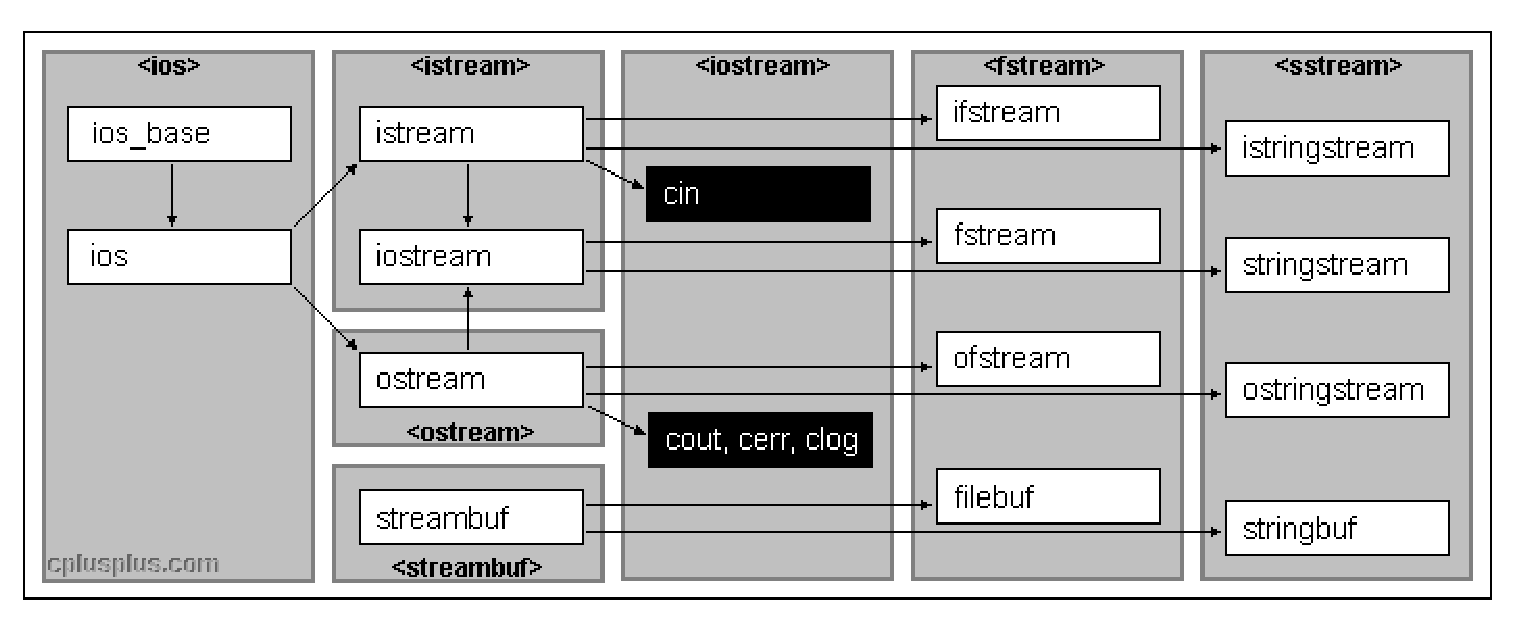
\includegraphics[height=5cm,
    angle=0]{./images/ios_hierarchy.eps}}
  \caption{}
  \label{fig:ios_hierarchy}
\end{figure}

The IO streams class hierarchy is given in Fig.\ref{fig:ios_hierarchy}.  An
important character of IO Stream is serial, we cannot make a random read or
random write to a string. Any built-in data types can be used with IO Streams'
APIs. To export values of user-defined data types, we need to override the {\bf
insertion operator} \verb!<<! to tell how to put objects into the stream, and
the {\bf extraction operator} \verb!>>! to tell how to read objects from the
stream. We can use 
\begin{verbatim}
#include <iostream>
using namespace std;


std::cout << "String to print out"
          << "another line to print out" 
          << std::endl;
\end{verbatim}


To format the parametric output, we use \verb!<iomanip>! (io manipulation). Each
manipulator receives one single argument, and returns one of the six unspecified
type T1 to T6
\footnote{\url{http://publib.boulder.ibm.com/infocenter/comphelp/v9v111/index.jsp?topic=/com.ibm.xlcpp9.aix.doc/standlib/header_iomanip.htm}}
\begin{verbatim}
namespace std {
  T1 resetiosflags(ios_base::fmtflags mask);
  T2 setiosflags(ios_base::fmtflags mask);
  T3 setbase(int base);
     template<class E>
  T4 setfill(E c);
  T5 setprecision(streamsize n);
  T6 setw(streamsize n);
}
\end{verbatim}
\begin{itemize}
  \item How many decimal points to print out after '0'
  \begin{verbatim}
  54.271123 and used setprecision(2) it would print out: 54.27 to the console.
  
  \end{verbatim}
  
  \item
  \begin{verbatim}
cout << setiosflags(ios::fixed) << setiosflags(ios::showpoint);  
  \end{verbatim}
\end{itemize}

\subsection{basic\_streambuf}
\label{sec:basic_streambuf}

\verb!basic_streambfu! is the abstract class, with a number of virtual functions
which are overridden to provide a uniform interface for reading/writing files, strings, etc.

\subsection{pubsetbuf()}

The only required behavior is that stream->pubsetbuf(0, 0) makes the file buffer
unbuffered which you almost certainly don't want. It doesn't make any guarantees
what happens if the arguments are non-null.
In particular, it doesn't guarantee that the buffer being used is the one being
passed! 

\subsection{streambuf}
\label{sec:streambuf}

All stream operations are buffered, with the base class streambuf is used behind
the scenes. It is provided with its own buffer, which size is an implementation
detail.

The stream buffer only affect the maximum number of bytes transferred to or from
the kernel with one syscall. Thus, the ideal buffer size doesn't depend on how
much data you transfer. What is does depend on is

\begin{verbatim}
The overhead cost of syscalls. 
        Higher overhead means you'll want to transfer more data in one go.

The overhead cost of buffer management. Probably larger for larger buffers, if anything.

CPU cache trashing effects. Will strongly favour smaller buffers.
\end{verbatim}
Since (1) works in favour of larger buffers while (2) and (3) work in favour of
smaller buffers, there will be a sweet spot somewhere.


Buffering:

If by default the buffer is very small, increasing the buffer size can definitely improve the performance:

    it reduces the number of HDD hits
    it reduces the number of system calls

Buffer can be set by accessing the underlying streambuf implementation.

\begin{verbatim}
char Buffer[N];

std::ifstream file("file.txt");

file.rdbuf()->pubsetbuf(Buffer, N);
// the pointer reader by rdbuf is guaranteed
// to be non-null after successful constructor
\end{verbatim}


\subsection{ios::rdbuf vs. fstream::rdbuf}

\begin{verbatim}
get (1)	
         streambuf* rdbuf() const;

set (2)	
         streambuf* rdbuf (streambuf* sb);
\end{verbatim}
sets the object pointed by sb as the stream buffer associated with the stream


\subsection{ofstream}

An ofstream by default opens its buffer in output mode only, and either way
you're only passing \verb!std::ios_base::out!, which means the buffer cannot be
read from.

\begin{verbatim}
To fix this you will need to switch to using an fstream and open it with
std::ios_base::in | std::ios_base::out | std::ios_base::binary

You will also need to seek to the start of the file before calling rdbufby
calling seekg(0, std::ios_base::beg).
\end{verbatim}

Use ofstream when textfile is for output only, ifstream for input only, fstream
for both input and output


\subsection{I/O with <istream>, <ostream> or <iostream>: peek(), getline(),
read(), readsome(), ignore()}
\label{sec:iostream}


If we don't care the physical input is a file, a buffer string, or a
console, then we just declare the variable as \verb!std::istream! for input and
\verb!std::ostream! for output. 

\verb!ostream! classes are just wrappers around I/O buffers, and provide
\verb!operator>>! formatting operators. The buffer is provided by an object
derived from \verb!basic_streambuf! (Sect.\ref{sec:basic_streambuf}), which you
can get and set using rdbuf().


There are 2 ways to connect to a file
\begin{verbatim}
// Option 1:
std::ifstream is ("test.txt", std::ifstream::binary);

// Option 2:
std::filebuf fb;
  if (fb.open ("test.txt",std::ios::in))
  {
    std::istream is(&fb);
    while (is)
      std::cout << char(is.get());
    fb.close();
  }
\end{verbatim}
then we can use proper methods to extract data in the form of single character,
a string or a block of data.

It has important functions that can be used in the children classes
\footnote{\url{http://www.cplusplus.com/reference/istream/istream/}}
\begin{itemize}
  \item Read but DON'T extract from the stream
  \begin{verbatim}
  int peek();
  \end{verbatim}
  Read the next character, without extracting. This is useful when you want to
  do parsing
  
  \item Extract character (using C++ string, i.e. you don't have to guess or
  specify the size of the pre-allocate buffer). However, if you read in a file,
  without specifying a \verb!delim! and there is no newline character in the
  file, then \verb!bad_alloc! error may occur.
  \begin{verbatim}
istream& std::getline (istream& is, string& str, char delim);
istream& std::getline (istream& is, string& str);
  \end{verbatim}
which extracts the content from \verb!is! and stores to \verb!str!, until a
delimiter is found (default=newline). NOTE: The delimiter, if found, is
extracted from the stream and is discarded, i.e. not store in \verb!str!.
  
  \item Extract characters (using C-style string):
  \begin{verbatim}
istream& std::istream::getline (char* s, streamsize n );
istream& std::istream::getline (char* s, streamsize n, char delim );
  \end{verbatim}
Extract characters and store them as C-style string \verb!s!, until 
\begin{itemize}
  \item a delimiter is read (default is newline \verb!'\n'!) or 
  \item $n-1$ characters has been read, and written \verb!s! (the $n$-th
  character is the \verb!null! character which is appended automatically)
  \item the end-of-file is reached, , if this occurs first, the \verb!eofbit!
  flag is set.
\end{itemize}
whichever first. A \verb!null! character (\verb!'\0'!) is automatically
appended, even if an empty string is returned.

If you want to be more flexible, you should use \verb!get()! method, which can
does what \verb!getline()! does, and more options: (1) extract a single
character, (2) put to the streambuffer.

  \item Read a block of data from the input (without checking the content nor
  appending NULL character at the end).
  \begin{verbatim}
  istream& istream::read (char* s, streamsize n);
  streamsize istream::readsome (char* s, streamsize n);
  \end{verbatim}
  extract up to $n$ characters, and store them into the array pointed by $s$.
  \verb!readsome()! is designed to work with some types of asynchronous sources
  that may eventually wait for more characters, as the function return as soon
  as the internal buffer is exhausted, i.e. avoiding potential delays.
  
  \item Extract from the input sequence, but discard them, until (whichever
  come first) $n$ characters or a delimiter is read. Default delimiter is EOF
  (end-of-file)
  \begin{verbatim}
  istream& ignore (streamsize n = 1, int delim = EOF);
  \end{verbatim}
  to focus on the delimiter, i.e. ignore as many as possible, we use 
  \begin{lstlisting}
  #include <limist>
  
  file.ignore(std::numeric_limits<std::streamsize>::max(), '}');
  \end{lstlisting}
  
  
  \item Return the number of characters read by the last {\it unformatted input
  operations} called by : \verb!get!, \verb!getline()!, \verb!read!, or
  \verb!readsome()!
  \begin{verbatim}
  streamsize gcount() const;
  \end{verbatim}
\end{itemize}

For output, similarly, we can use \verb!<ostream>!. And if we want to use the
stream for both input + output, we declare it as \verb!<iostream>!.

\subsection{File I/O with <fstream>, <ifstream>, <ofstream>}
\label{sec:std::fstream}

STL also incldue <fstream> which contains input and output stream classes.
\begin{enumerate}
  \item for input only: \verb!ifstream! class
  \item for output only: \verb!ofstream! class
  \item for input + output: \verb!fstream! class. There's an internal buffer
  object calls {\bf filebuf} that performs input/output  operations on the file
  it's associated with.   
\end{enumerate}
% NOTE: std::ifstream is INEFFICIENT compared to fread. The reason is that
% \verb!fread()! put the whole file into memory. So after \verb!fread()!,
% accessing the buffer is faster. 
Beside the standard way to open a file using \verb!.open()! member function, we
can also directly pass the filename when defining the ofstream object.
However, in C++98, the only way to open a file-stream by passing the filename is
to convert to C-style string.
\begin{verbatim}
	std::string filename("text.out");
#if defined(__CXX_EXPERIMENTAL_CXX0X__) || __cplusplus >= 201103L
	std::ofstream ofile(filename);
#else
	std::ofstream ofile(filename.c_str());
#endif	
\end{verbatim}

Another important thing is in C++11, \verb!ofstream! is movable. 

Example: \verb!ifstream:read()! is buffered, and we just tell how much data we
need to read in each time

{\small \begin{verbatim} 
void readFile()
{
    std::ifstream fin;
    fin.open("largefile.dat", ifstream::binary | ifstream::in);
    // in each of these small read methods, there are at least 1 fin.read()
    // call inside.
    readHeaderInfo(fin);
    readPreference(fin);
    readMainContent(fin);
    readVolumeData(fin);
    readTextureData(fin);
    fin.close();
}
\end{verbatim}}

TIPS: Use fread()/fwrite() for binary. maximize chunk size. Use fstreams for
ascii i/o. The best thing around is stream.getline() which saves you any string
ops if you want to extract data by newline (or any other delimiter). 

{\small \begin{verbatim} 
#include <iostream>
#include <fstream>
#include <streambuf>

ofstream ofs("file.txt" );
streambuf* original = cout.rdbuf();
cout.rdbuf( ofs.rdbuf() );  // cout now writes to the file

...

cout.rdbuf( original );  // MUST restore before quitting
\end{verbatim}}

\subsection{Temporay file}
\label{sec:temporary_file}

\verb!std::tmpfile! creates temporary binary file, open for update (``+wb''
mode). The filename is selected by the system, with guarantee that it's
different from any other existing files in the system.
\begin{verbatim}
FILE *pFile;
pFile = tmpfile ( void ); //the pointer to temporary file handle
 
 //work with pFile

fclose(pFile);
\end{verbatim}

To close and also delete the file, we use \verb!fclose(FILE*)!.  If the programs
terminate normally, whether the files are removed depends on the
library implementation.


We can use \verb!ostream!
\begin{verbatim}
char *tmpname = strdup("/tmp/tmpfileXXXXXX");
mkstemp(tmpname);
ofstream f(tmpname);
\end{verbatim}
NOTE: \verb!mkstemp()! can fail and return -1. So the code should catch that
case.

Here is another way
\begin{verbatim}
#include <stdlib.h>
#include <fstream>
#include <iostream>
#include <vector>

std::string open_temp(std::string path, std::ofstream& f) {
    path += "/XXXXXX";
    std::vector<char> dst_path(path.begin(), path.end());
    dst_path.push_back('\0');

    int fd = mkstemp(&dst_path[0]);
    if(fd != -1) {
        path.assign(dst_path.begin(), dst_path.end() - 1);
        f.open(path.c_str(), 
               std::ios_base::trunc | std::ios_base::out);
        close(fd);
    }
    return path;
}

int main() {
    std::ofstream logfile;
    open_temp("/tmp", logfile);
    if(logfile.is_open()) {
        logfile << "hello, dude" << std::endl;
    }
}
\end{verbatim}

References:
\begin{enumerate}
  \item \url{http://www.cplusplus.com/reference/cstdio/tmpfile/}
  
  \item
  \url{http://stackoverflow.com/questions/499636/how-to-create-a-stdofstream-to-a-temp-file}
\end{enumerate}

\subsection{Using user-defined set of routines}

We define a struct that keep the file-handle and file-name.
\begin{verbatim}
typedef struct {
   FILE* file;
   char* name;
} OBJECTFILE
\end{verbatim}

Then, we write a function to open a file \verb!object_fopen()!
\begin{verbatim}
OBJECTFILE file;
file = object_fopen(filename, "r")
\end{verbatim}
with
\begin{verbatim}
OBJECTFILE
object_fopen(const char* filename, char *mode)
{
  OBJECTFILE file;
  file.file = fopen(filename, mode);
  if (file.file == NULL) {
     char *msg;
     int msg_length;
     msg_length = strlen(filename) + 256;
     msg = (char*) Mallloc(msg_length);
     sprintf (msg, "%d: Error opening file=%s with mode %s from object_fopen",
        getRank(0), filename, mode);
     perror(msg);
     Free(msg);
  }
  
  filename = strdup(filename);
  return file;
}

void object_fclose(OBJECTFILE file)
{
  fclose(file.file);
  Free(file.name);
}   

char* object_read(OBJECTFILE file)
{  
}  
\end{verbatim}

\subsection{istringstream}

A stringstream is basically a string, but you can read/write data to it easily
using \verb!<<! and \verb!>>! operator, just like working with file or
\verb!std:cin!.

A stringstream works essentially like an input/output file stream. The
header file required is \verb!<sstream>!. To declare a stringstream, we do
\begin{verbatim}
#include <sstream>

stringstream ss;
\end{verbatim}

We can write to it or read from it using \verb!<<! or \verb!>>! operator
\begin{verbatim}
std::string myString;
char myChar;

ss << mychar ;
ss << myString;

int myInt;

ss >> myInt;
\end{verbatim}
Example:
\begin{lstlisting}
std::string s = "1 2 3"; // this is the original string
std::istringstream is(s); // this istringstream contains a copy of s
int i,j,k; // variables to write to
is >> i >> j >> k; // now i is 1, j is 2, and k is 3
\end{lstlisting}

To convert the entire stringstream to string
\begin{verbatim}
std::string str = ss.str();
\end{verbatim}


Other member functions from stream can be used with stringstream like
\verb!get!, \verb!getline()!, \verb!read!, \verb!write!, \verb!put()!


\section{Boost::Spirit.Karma (Output)}
\label{sec:boost_spirit_Karma}

Typically, \verb!printf, std::stream! formatting, or \verb!boost::format! have
been used for formatting output data. However, for complicated data structure,
it's hard to develop codes for writing data with proper format. A solution is
using \verb!Spirit.Karma! package from Boost::Spirit library. 


This is in opposite of Spirit::Qi which parse the input data from files into
internal data structure (Sect.\ref{sec:boost_spirit_Qi}).

\section{Boost::Spirit::Qi (Input)}
\label{sec:boost_spirit_Qi}

This is the parser library that we use to build recursive descent parsers
(Sect.\ref{sec:boost_spirit}).

Example:
\url{http://www.codeproject.com/Articles/8516/An-Introduction-to-the-Boost-Spirit-Parser-framewo}
We define a grammar class or struct, by inheriting \verb!boost::spirit::grammar!
class. In this class/struct, say \verb!MyGrammar!, we need to define a nested
struct called \verb!definition! (containing the language description that you
want to parse, i.e. a number of rules, ), and a member function call
\verb!start()! (returning the start rule).


\section{Boost::Spirit::Classic (Input)}
\label{sec:boost_spirit_classic}

This is considered depricated and we should use Boost::Spirit::Qi.

\url{http://www.codeproject.com/Articles/8516/An-Introduction-to-the-Boost-Spirit-Parser-framewo}

\url{http://www.codeproject.com/Articles/8522/Implementing-Semantic-Actions-in-the-Boost-Spirit}

{\small \begin{verbatim} 
struct MyGrammar :
    public boost::spirit::grammar<MyGrammar>
{
public:
    MyGrammar( CParser &parser );
    virtual ~MyGrammar();
    template <typename ScannerT>
    struct definition
    {
    public:
        definition( MyGrammar const &self )
        {
            integer =
                lexeme_d[ (+digit_p) ]
                ;
            factor =
                integer |
                vars |
                '(' >> expression >> ')' |
                ( '-' >> factor ) |
                ( '+' >> factor )
                ;
            term =
                factor >> *( ( '*' >> factor) | ( '/' >> factor ) )
                ;
            expression =
                term >> *( ( '+' >> term ) | ( '-' >> term ) )
                ;
            assignment =
                vars
                >> '=' >> expression
                ;
            var_decl =
                lexeme_d
                [
                    ( ( alpha_p >> *( alnum_p | '_' ) )
                    - vars )[vars.add]
                ]
                ;
            declaration =
                "int" >> var_decl >> *( ',' >> var_decl )
                ;
            baseExpression =
                str_p( "exit" )[*self.m_finishedProcessing] |
                str_p( "mod" ) >> integer |
                declaration |
                assignment |
                '?' >> expression
                ;
        }
        boost::spirit::symbols<int> vars;
        boost::spirit::rule<ScannerT> integer, factor, term,
            expression, assignment, var_decl, declaration,
            baseExpression;
        const boost::spirit::rule<ScannerT> &start() const { return baseExpression; }
    };
    friend struct definition;
private:
    Private::FinishedProcessing *m_finishedProcessing;
};
\end{verbatim}}

NOTE: The grammar is described using EBNF rules.
\begin{itemize}
  \item \verb!lexeme_d!: directive to tell the parser NOT to skip white spaces
  \item \verb!+digit_p!: directive to tell matching one or more numeric
  characters
  \item All the rules defined in the \verb!definition! struct, must also be
  defined in the class \verb!MyGrammar! of type
  \verb!boost::spirit::rule<ScannerT>!.
  \begin{verbatim}
        boost::spirit::rule<ScannerT> integer, factor, term,
            expression, assignment, var_decl, declaration,
            baseExpression;  
  \end{verbatim}
  \item The \verb!start()! function returns the entry point rule,
  i.e. baseExpression.
\end{itemize}

Now, after you have read-in the code in the form of a single string, we give it
to the parser.
\begin{verbatim}
//read-in input-file
//storing the content in 'line' string.

boost::spirit::parse_info<> info;
MyGrammar parser;
info = boost::spirit::parse( line.c_str(), parser, boost::spirit::space_p );
\end{verbatim}
NOTE: We can pass a string, or a pair of iterators for begin and end.



\section{Clang: parsing C/C++/Objective-C/Objective-C++ code}

{\bf Clang} is a powerful, free parser that can be used as a front-end for a
compiler \footnote{\url{http://clang.llvm.org/index.html}}. 

\section{Check file status}

We use the \verb!struct stat! structure which is a system struct that is
defined to store information about a given file. There are different field in
this structure. \url{http://codewiki.wikidot.com/c:struct-stat}

 {\small 
\begin{verbatim}
#include <iostream>
#include <sys/types.h>
#include <sys/stat.h>
#include <fcntl.h>
#include <string>
 using namespace std;

int main() {
     struct stat buf;
     std::string filename(``object.data'')
     stat(filename,&buf);

  cout << buf.st_dev << endl;     
 }
\end{verbatim}
}

Another way is to use \verb!filetest()!
\begin{verbatim}
#include <string>

std::string myfile("input.txt");

if (filetest(myfile.c_str(), S_IFREG) != 0) {
  cout << "File not exist";
}
\end{verbatim}

\section{Serialization (copying object's state)}
\label{sec:Serialization_C_C++}

The process to translate data structure or object state into the format that can
be stored (to harddrive), transfered (via network) and then resurrected later is
called {\bf serialization} (deflating, marshalling). This process is not trivial
if the object has extensive use of references. The reverse process, extracting
data structure from a series of bytes is called {\bf deserialization}
(inflating, unmarshalling).

A serialization need to provide at least 4 methods
\begin{enumerate}
  \item to write the object's data to a file or database
  \item to do RPC (remote-procedure call)
  \item to distribute the object
  \item to detect changes in time-varying data
\end{enumerate}
As we need to transfer the data across network, the implementation need to be
portable, i.e. users don't need to concern about byte-ordering, memory layout,
etc.

Serialization, however, breaks the opacity of abstract data type, i.e. you need
to expose private data member (i.e. data encapsulation).

\textcolor{red}{C/C++ do NOT provide direct support to serialization}. However, you can write
your own code for serialization. MFC (Microsoft Foundation Class) library also
provides serialization support. Another library is Boost.Serialization.

\subsection{Boost.Serialization}

The output file format can be: ASCII, XML, binary. The advantage of XML is
useful in debugging. Also, this format is propertary, so you cannot use it to
exchange data with application that doesn't use Boost.Serialization.

You have a simple class:
\begin{verbatim}
/////////////////////////////////////////////////////////////
// gps coordinate
//
// illustrates serialization for a simple type
//
class gps_position
{
private:
    int degrees;
    int minutes;
    float seconds;
public:
    gps_position(){};
    gps_position(int d, int m, float s) :
        degrees(d), minutes(m), seconds(s)
    {}
};
\end{verbatim}

The main concept of Boost.Serialization is an {\bf archive}, which is a sequence
of bytes representing serialized C++ objects. It means that an object can be
loaded into the archive to be serialize from them or to be loaded from it. 
To save the C++ object state to an archive which connect to a particular output
\begin{verbatim}
// Output archive as text stream.
// Even though it's not a stream, it can be used like a stream via << operator
#include <boost/archive/text_oarchive.hpp> 

// save the archive to standard output
boost::archive::text_oarchive oa(std::cout); 
\end{verbatim}


To restore object data from an archive which reads from file, we can use
\begin{verbatim}
#include <boost/archive/text_iarchive.hpp> 

//read from a text file
std::ofstream file("archiv.txt"); 
boost::archive::text_oarchive oa(file); 
\end{verbatim}


\subsubsection{If you can change the class definition}

You need to modify the class and a method name \verb!serialize()! must be
defined. This method is used for both serializing and restoring. The method
should never be called explicitly, and thus should be declared as private, and
the class \verb!boost::serialization::access! is declared as friend.

\begin{verbatim}
class gps_position
{
private:
    friend class boost::serialization::access;
    
    // When the class Archive corresponds to an output archive, the
    // & operator is defined similar to <<.  Likewise, when the class Archive
    // is a type of input archive the & operator is defined similar to >>.
    template<class Archive>
    void serialize(Archive & ar, const unsigned int version)
    {
        ar & degrees;
        ar & minutes;
        ar & seconds;
    }
...
}
\end{verbatim}

Then to save to text file and to restore the class data
\begin{verbatim}
#include <boost/archive/text_oarchive.hpp>
#include <boost/archive/text_iarchive.hpp>


int main() {
    // create and open a character archive for output
    std::ofstream ofs("filename");

    // create class instance
    const gps_position g(35, 59, 24.567f);

    // save data to archive
    {
        boost::archive::text_oarchive oa(ofs);
        // write class instance to archive
        oa << g;
    	// archive and stream closed when destructors are called
    }

    // ... some time later restore the class instance to its orginal state
    gps_position newg;
    {
        // create and open an archive for input
        std::ifstream ifs("filename");
        boost::archive::text_iarchive ia(ifs);
        // read class state from archive
        ia >> newg;
        // archive and stream closed when destructors are called
    }
    return 0;
}
\end{verbatim}

\subsubsection{If you can't (don't want to) change the class definition}

It means the class doesn't have to be derived from a specific class or implement
a specified member function.

You first need to make all data member public or make the class expose enough
information to reconstruct the class state.
\begin{verbatim}
class gps_position
{
public:
    int degrees;
    int minutes;
    float seconds;
    gps_position(){};
    gps_position(int d, int m, float s) :
        degrees(d), minutes(m), seconds(s)
    {}
};
\end{verbatim}

And then define a new member for Boost.Serialization
\begin{verbatim}
namespace boost {
namespace serialization {

template<class Archive>
void serialize(Archive & ar, gps_position & g, const unsigned int version)
{
//put any data member you want to output here
    ar & g.degrees;
    ar & g.minutes;
    ar & g.seconds;
}

} // namespace serialization
} // namespace boost
\end{verbatim}

Typically, we define two function \verb!save()! and \verb!load()!
\begin{verbatim}
void save() 
{ 
  boost::archive::text_oarchive oa(ss); 
  int i = 1; 
  oa << i; 
} 

void load() 
{ 
  boost::archive::text_iarchive ia(ss); 
  int i = 0; 
  ia >> i; 
  std::cout << i << std::endl; 
} 
\end{verbatim}

\subsubsection{Split load/save}

There are two cases: intrusive and non-intrusive approach:

\textcolor{red}{\bf Intrusive}: We need to include \verb!split_member.hpp!
header file, and then define two separate method \verb!save()! and \verb!load()!
to split the serialization into 2 separate functions.

\begin{verbatim}
#include <boost/serialization/split_member.hpp>
 
template<class Archive>
void save(Archive & ar, const unsigned int version) const
{
    // invoke serialization of the base class 
    ar << boost::serialization::base_object<const base_class_of_T>(*this);
    ar << member1;
    ar << member2;
    ar << member3;
}

template<class Archive>
void load(Archive & ar, const unsigned int version)
{
    // invoke serialization of the base class 
    ar >> boost::serialization::base_object<base_class_of_T>(*this);
    ar >> member1;
    ar >> member2;
    if(version > 0)
        ar >> member3;
}

template<class Archive>
void serialize(
    Archive & ar,
    const unsigned int file_version 
){
    boost::serialization::split_member(ar, *this, file_version);
}
\end{verbatim}

\textcolor{red}{\bf Non-intrusive}: 

We need to include \verb!split_free.hpp! file,
\begin{verbatim}
#include < boost/serialization/split_free.hpp>

namespace boost { namespace serialization {

template<class Archive>
inline void serialize(
    Archive & ar,
    my_class & t,
    const unsigned int file_version
){
    split_free(ar, t, file_version); 
}
}}

\end{verbatim}

\subsubsection{Data member as reference/pointer}

In the \verb!serialize()! member function we have
\begin{verbatim}
{
    // save/load class member variables
    ar & member1;
    ar & member2;
}
\end{verbatim}

If it's for a children class, we have
\begin{verbatim}
{
    // invoke serialization of the base class 
    ar & boost::serialization::base_object<base_class_of_T>(*this);
    // save/load class member variables
    ar & member1;
    ar & member2;
}
\end{verbatim}

If you have a data member which is a reference or a pointer, then how and where
the object being referred to are stored and how they are created, e.g.
\verb!member! data member in our case. REMEMBER: reference is a special kind of
pointer, so we serialize the reference as though it is a pointer 
\begin{verbatim}
class object;
class my_class {
private:
    friend class boost::serialization::access;
    int member1;
    object & member2;
    template<class Archive>
    void serialize(Archive &ar, const unsigned int file_version);
public:
    my_class(int m, object & o) :
        member1(m), 
        member2(o)
    {}
};
\end{verbatim}

Then we define an override
\begin{verbatim}
namespace boost { namespace serialization {
template<class Archive>
inline void save_construct_data(
    Archive & ar, const my_class * t, const unsigned int file_version
){
    // save data required to construct instance
    ar << t.member1;
    // serialize reference to object as a pointer
    ar << & t.member2;
}

template<class Archive>
inline void load_construct_data(
    Archive & ar, my_class * t, const unsigned int file_version
){
    // retrieve data from archive required to construct new instance
    int m;
    ar >> m;
    // create and load data through pointer to object
    // tracking handles issues of duplicates.
    object * optr;
    ar >> optr;
    // invoke inplace constructor to initialize instance of my_class
    ::new(t)my_class(m, *optr);
}
}} // namespace ...
\end{verbatim}


\subsubsection{Class versioning}

If we change the class definition, we can use version to determine how to load
the data. When we serialize a class, we have the option to pass the version
information to it.

When it is loaded from the archive, the version number is passed as an argument
to the loading function, we can check using \verb!file_version!
\begin{verbatim}
{
    // invoke serialization of the base class 
    ar & boost::serialization::base_object<base_class_of_T>(*this);
    // save/load class member variables
    ar & member1;
    ar & member2;
    // if its a recent version of the class
    if(1 < file_version)
        // save load recently added class members
        ar & member3;
}
\end{verbatim}

\subsubsection{Using XML}

\begin{verbatim}
boost::archive::xml_oarchive xmlArchive(oStringStream);

xmlArchive.register_type(static_cast<BaseMessage *>(NULL));
xmlArchive.register_type(static_cast<IncomingTradeMessage *>(NULL));
xmlArchive.register_type(static_cast<InternalRequestInfo *>(NULL));
xmlArchive.register_type(static_cast<InternalTradeTransInfo *>(NULL));

const BaseMessage* myMessage =message;

xmlArchive << make_nvp("Message", myMessage);
\end{verbatim}

\subsubsection{Inheritance}

How Boost.Serialization know the class of the object it serializes has a parent,
or even what that parent is.

\begin{lstlisting}
class MyParent {
public:
	
private:
	int ID;
    friend class boost::serialization::access;
    
	template<class Archive> void serialize(Archive& ar,
       const unsigned int version) 
    {
		ar & BOOST_SERIALIZATION_NVP(ID);
	}	
\end{lstlisting}

\begin{lstlisting}
class ChildClass :: MyParent 
{
public:

private:
	friend class boost::serialization::access;
    template<class Archive> void serialize(Archive& ar,
        const unsigned int version) {
          
           /// what should be here???
           /// check below
    }
}
\end{lstlisting}


To serialize the childen class, we need to tell the compiler 
what the object's parent is and provide a reference to it, you can put this line
at the beginning or the end of the \verb!serialize()! member function of the
children class, depening on how you want to structure the output
\begin{verbatim}
ar & boost::serialization::make_nvp("MyParent",
     boost::serialization::base_object<MyParent>(*this))
\end{verbatim}
\url{http://stuartjames.info/Journal/boost-serialization-for-inherited-objects.aspx}

Another option: the children class need have access to
\verb!boost::serialization::base_object()! function inside the
\verb!serialize()! method.
\begin{verbatim}
#include <fstream>
#include <boost/serialization/export.hpp>
#include <boost/archive/text_oarchive.hpp>

class Foo {
    friend class boost::serialization::access;

    template<class Archive>
    void serialize(Archive & ar, const unsigned int version)
    {
        ar & dummy1;
    }

    int dummy1;

public:
    virtual ~Foo() {}
};


class Bar : public Foo {
    friend class boost::serialization::access;

    template<class Archive>
    void serialize(Archive & ar, const unsigned int version)
    {
        // serialize base class information
        ar & boost::serialization::base_object<Foo>(*this);
        ar & dummy2;
    }

    int dummy2;
};

BOOST_CLASS_EXPORT_GUID(Foo, "Foo")
BOOST_CLASS_EXPORT_GUID(Bar, "Bar")

int main(int argc, char *argv[]) {
    std::ofstream ofs("filename");
    boost::archive::text_oarchive oa(ofs);
    Foo *f = new Bar;
    oa << f;

    return 0;
}
\end{verbatim}

\subsection{ACCU}

\url{http://accu.org/index.php/journals/486}


\section{UTF-16 file data}


\subsection{Library: ICU}
\label{sec:ICU}


International Components for Unicode (ICU) provides a cross-platform,
Unicode-based globalization for handling text data in any formats
\footnote{\url{http://site.icu-project.org/home}}.

\begin{itemize}
  \item convert text data to/from Unicode and nearly any other character sets
  \item compare string: based on Unicode Collation Algorithm plus
  locale-specific comparison rules.
  
  \item format string that represents numbers, date, times, currency according
  to a chosen locale.
  \item regular expression: able to handling text left-to-right (English) or
  light-to-left (Arabic, Hebrew) data
  \item text boundaries: 
\end{itemize}

\begin{mdframed}
Why not using ICU?
\begin{itemize}
  \item APIs do not follow modern C++ design, and do not work well with
  newer versions of standard C++ library
  (Sect.\ref{sec:standard-C++-library})
  
  \item UTF-16 oriented. No support for narrow encoding (e.g. ISO 8859)
  
  \item Message translation tool is far from perfect, which can be done with
  GNU \verb!Gettext! model in Boost.Locale (Sect.\ref{sec:Boost.Locale})
  
\end{itemize}

Why using ICU?
\begin{itemize}
  \item one of the best localization/Unicode libraries available
  \item 
\end{itemize}
\end{mdframed}


Compile and install the library before using:
\footnote{\url{http://stuf.ro/reading-a-utf-8-file-in-c-with-icu}}
\begin{verbatim}
// we use -E -H to preserve the environment variables in 'sudo' mode
./configure --enable-static --prefix=/usr && make && sudo -E -H make install

/* statically linking (need to use g++ even for C-code) */
g++ main.c -o main.o -static -lsicuio -lsicui18n -lsicuuc -lsicudata

/* dynamically linking */
gcc main.c -o main.o `icu-config --ld-flags --ld-flags-icuio`
\end{verbatim}


The new data type is \verb!UChar*!, and string operating functions is the same
as C-library except with a prefix \verb!u_!, e.g. \verb!u_printf, u_fclose!. To
allocate and free the string, the function doesn't change, \verb!free()!.
\begin{verbatim}
UChar* str = (UChar*) malloc(sizeof(UChar) * (fsize + 1));
\end{verbatim}

The file object is \verb!UFILE!, with \verb!u_fopen(), u_fclose()! functions.

Example:
\begin{Verbatim}
#include <stdio.h>
#include <stdlib.h>

#include "unicode/ustdio.h"
#include "unicode/uchar.h"

/**
 * Reads a UTF-8 file and returns an UChar array containing the string read.
 *
 * @param filename the path to the file to be read
 * @param size pointer to a variable in which to store the UTF-8 string length
 *
 * @return UTF-8 string (dynamically allocated; must be freed after usage)
 */
UChar* read_utf8_file(const char* filename, long* size) {
    /* open a UTF-8 file for reading */
    UFILE* f = u_fopen(filename, "r", NULL, "UTF-8");

    /* get the file size */
    long fsize;
    fseek(u_fgetfile(f), 0, SEEK_END);
    fsize = ftell(u_fgetfile(f));
    u_frewind(f);

    /* allocate enough memory to store the whole string plus termination */
    UChar* str = (UChar*) malloc(sizeof(UChar) * (fsize + 1));

    /* read the string into the allocated space */
    for ((*size) = 0; !u_feof(f); ++(*size)) {
        str[*size] = u_fgetc(f);
    }

    /* add NULL termination */
    str[*size] = 0;

    /* close the file resource */
    u_fclose(f);

    return str;
}

int main() {
    /* read the string and its size */
    long size;
    UChar* str = read_utf8_file("utf8_test.txt", &size);

    /* print the string size */
    printf("String size: %ld\n\n", size);

    /* print the UTF-8 string */
    UFILE* u_stdout = u_finit(stdout, NULL, NULL);
    u_fprintf(u_stdout, "%S\n", str);
    u_fclose(u_stdout);

    /* free the allocated string */
    free(str);

    return 0;
}
\end{Verbatim}
\section{UTF-8 file data}

If the file is encoded in UTF-8.

\subsection{Microsoft VC++}
\label{sec:wide-character_VC++}

In Microsoft Visual C++ 2005, we can use \verb!fgets()! to decode UTF-8 encoded
file when we create the stream using an extension \verb!ccs=encoding! to open file using
FILE object (Sect.\ref{sec:C-stream-IO}). However, in Visual C++ 2005, this only
work for opening only, not for writing. Other encoded types are also supported
\begin{verbatim}
"ccs=UNICODE" => UTF-16 (Big endian)
"ccs=UTF-8" => UTF-8
"ccs=UTF-16LE" => UTFS-16LE (Little endian) 
"ccs=ANSI" => ANSI (default encoding of the OS)
\end{verbatim}

%wchar_t* unicode_text = L"こんにちは";
Example: reading in
\begin{verbatim}
wchar_t* unicode_text[100];
FILE* f = fopen("C:\\test.txt", "w,ccs=UTF-8");
// fwprintf(f, L"%s\n", unicode_text);
fgets(f, unicode_text);
fclose(f);
\end{verbatim}


For reading in, if you know the locale, you can set with \verb!locale()!
\begin{verbatim}

wchar_t buffer[1000];
FILE* f = fopen("C:\\test.txt", "r");
fgetws(buffer, 1000, f);
fclose(f);

//MessageBoxW(0, buffer, 0, 0);
wprintf (L"% s ", buffer)
\end{verbatim}
Use \verb!fgetws()! to read-in wide-character string.

\subsection{Boost.Locale}
\label{sec:Boost.Locale}

\url{http://www.boost.org/doc/libs/1_55_0/libs/locale/doc/html/index.html}

Boost.Locale connect C++ locale framework, isostreams, and the powerful ICU
library (Sect.\ref{sec:ICU}). Also, Boost.Locale provide non-ICU localization
support.

As ICU is huge (half a million lines of well-tested code), Boost.Locale only
wraps ICU with a modern C++ interface. The entire ICU is hidden behind opaque
pointer and users have no access to it.
  
\chapter{Files/Folders}

\url{http://www.gnu.org/software/libc/manual/html_node/File-System-Interface.html}

\section{Check file/folder existence and create/delete}

\subsection{struct stat (C) and mkdir() - Linux}

\verb!struct stat! is a system struct that is defined to store information about
files. The struct has different fields
\begin{verbatim}
#include <sys/stat.h>

struct stat buf;
it error_code = stat("filename.txt", &buf); //buf contains information

if (rc >= 0) 
{ //file exist
  
}
\end{verbatim}

NOTE:  The "sysstat.h" header deals with broken versions of <sys/stat.h> and can
be replaced by <sys/stat.h> on modern Unix systems (but there were many issues
back in 1990).

Example 2:
\begin{verbatim}
#include <sys/types.h>
#include <sys/stat.h>
#include <unistd.h>

struct stat st = {0};

if (stat("/some/directory", &st) == -1) {
    mkdir("/some/directory", 0700);
}
\end{verbatim}



\subsection{SHCreateDirectoryEX  (Win32/C++, Windows XP, 2003)}

In pure Win32/C++ and for Windows XP and 2003 only
\begin{verbatim}
inline void EnsureDirExists(const std::wstring& fullDirPath)
{
    HWND hwnd = NULL;
    const SECURITY_ATTRIBUTES *psa = NULL;
    int retval = SHCreateDirectoryEx(hwnd, fullDirPath.c_str(), psa);
    if (retval == ERROR_SUCCESS || retval == ERROR_FILE_EXISTS || retval == ERROR_ALREADY_EXISTS)
        return; //success

    throw boost::str(boost::wformat(L"Error accessing directory path: %1%; win32 error code: %2%") 
        % fullDirPath
        % boost::lexical_cast<std::wstring>(retval));

    //TODO *djg* must do error handling here, this can fail for permissions and that sort of thing
}
\end{verbatim}
\url{http://stackoverflow.com/questions/1680836/create-directory-sub-directories}

\subsection{<filesystem> header: VS C++ 2012}

The <filesystem> header is not part of C++11; it is a proposal for C++ TR2 based
on the Boost.Filesystem library. Visual C++ 2012 includes an implementation of
the proposed library.


\subsection{Boost.Filesystem V2 (cross-platform)}
\label{sec:boost_filesystem_V2}

This is outdated, use V3 instead (Sect.\ref{sec:boost_filesystem_V3}).
\verb!Boost.Filesystem! provides a convenient and cross-platform interface for
file and directory traversing and manipulation. The intent is not to compete
with Python/Perl/ or shell script, but to provide C++ the feature to do when
it's needed. We need to install this as a separately compiled library
\begin{verbatim}
#include "boost/filesystem.hpp"
using boost::filesystem; //or

namespace fs=boost::filesystem;
\end{verbatim}
and compile with
\begin{verbatim}
-I$BOOST_INCLUDE_DIR -L$BOOST_LIB_DIR -lboost_system lboost_filesystem
\end{verbatim}

A class \verb!path! object
\begin{verbatim}
// use either regular or wide-character
// Input : const char* 
//         const std::string &
path my_path("some_dir/file.txt");  
wpath my_path("some_dir/file.txt"); 
   //both returns a path object 
  //that works for API of any operating system that accepts either
  // some_dir::file.txt
  // [some_dir]file.txt
  // some_dir/file.txt
  // etc.
\end{verbatim}
We can also use \verb!operator/! to append paths
\begin{verbatim}
ifstream file1( arg_path / "foo" / "bar");
ifstream file1( arg_path / "foo/bar");
\end{verbatim}

\begin{enumerate}
  \item if file/folder exists
\begin{verbatim}
if (fs::exists(fs::status(data_dir)))       // true - directory exists
if (fs::exists( data_dir ))     
\end{verbatim}  
which nees an argument of type boost::filesystem::path or something that is
implicitly convertible to it, e.g. std::string

Check subfolder
\begin{verbatim}

boost::filesystem::path config_folder(Config::CONFIG_FOLDER_NAME);

//use / operator
if(!(boost::filesystem::exists(
    config_folder / Config::fmap[Config::current_hash_function]));

//or 
if( !(boost::filesystem::exists(
   std::string(boost::format("%s/%s") 
   % config_folder 
   % Config::fmap[Config::current_hash_function])));
{
\end{verbatim}

  \item create directory
\begin{verbatim}
create_directory("my_directory");
\end{verbatim}  
  \item remove
\begin{verbatim}
remove_all ("something");
\end{verbatim}

  \item copy file/folder
\begin{verbatim}
//NOTE: We should provide destination filename, 
//      not just the folder
path user_path( "C:\\My Folder" );
path dest_file( "C:\\My Folder\\file.txt" );

boost::filesystem::create_directory( user_path );
path file(  "C:\\Another\\file.txt" );

//WRONG
boost::filesystem::copy_file( file, user_path );
//CORRECT
boost::filesystem::copy_file( file, dest_file );
\end{verbatim}  

However, an exception is thrown if the file existed in the destination folder.
To copy with overwrite
\begin{verbatim}
fs::copy_file(sourcefile, destfile, fs::copy_option::overwrite_if_exists);
\end{verbatim}
NOTE: In older version of Boost 1.46 (before rev.67067), the problem is that 
if the dest file exists and is smaller than the source, then the function only
overwrite the first \verb!size(filesource)! bytes in the target file.

Another choice
\begin{verbatim}
if (exists (destfile))
	remove(destfile);
copy_file(sourcefile, destfile);	
\end{verbatim}
However, this raises the problem if the two files are the same??? If we delete
the target file then we also delete the source file.

Or to use try..catch
\begin{verbatim}
try
{
	fs::copy_file(sourcefile, destfile);
}catch (const fs::filesystem_error& e)
{
	std::cerr << "Error: " << e.what() << std::endl;
}
\end{verbatim}

   \item iterate through files
   
   \item find files
\begin{verbatim}
find_files
\end{verbatim}
\end{enumerate}


Even though it's not part of C++11; yet it's a proposal for C++11/TR2
\footnote{\url{www.open-std.org/jtc1/sc22/wg21/docs/papers/2012/n3335.html}}.
Visual C++2012 contains the implementation for this proposed library.

References:
\begin{enumerate}
  \item \url{www.boost.org/doc/libs/1_41_0/libs/filesystem/doc/index.htm}
\end{enumerate}

\subsection{Boost.Filesystem V3 (cross-platform, C++11)}
\label{sec:boost_filesystem_V3}

This is the major revision of Boost.Filesystem V2
(Sect.\ref{sec:boost_filesystem_V2}) to work better with C++11 new data type
\verb!char16_t! and \verb!char32_t!
\footnote{\url{www.boost.org/doc/libs/1_49_0/libs/filesystem/v3/doc/v3_design.html}}.
Boost.Filesystem V3 is the default in Boost 1.60.0+.

In this version, there's no need to use \verb!path! and \verb!wpath!, we only
need a single class \verb!path! that supports different character type
(\verb!char!, \verb!wchar_t! \verb!char16_t!, \verb!char32_t!).
The class \verb!path! also have new members
\begin{verbatim}
has_stem()

has_extension()

is_absolute()

is_relative()

make_preferred()
\end{verbatim}
New or improved functions
\begin{verbatim}
absolute()

create_symlink()

read_symlink()

resize_file()

unique_path()
\end{verbatim}

To create folder:
\begin{verbatim}
#include <boost/filesystem.hpp>
//...
boost::filesystem::create_directories("/tmp/a/b/c");
\end{verbatim}
which returns \verb!true! is creating folder successfully; and \verb!false!
otherwise.


\begin{enumerate}
  \item
  \url{http://www.boost.org/doc/libs/1_49_0/libs/filesystem/v3/doc/v3.html}
  
  \item
  \url{http://www.boost.org/doc/libs/1_46_1/libs/filesystem/v3/doc/reference.html}
\end{enumerate}

\section{Temporary filename: tmpnam(), mkstemp()}
\label{sec:tmpnam}
\label{sec:mkstemp}
\label{sec:tmpfile}

\verb!std::tmpnam()! is defined in \verb!<cstdio>!:
\begin{verbatim}
char* tmpnam(char* filename);
\end{verbatim}
create a unique filename that is different from any currently existing file, and
the name is stored in the argument. \textcolor{red}{CONS: not thread-safe; it is possible (though with low chance) that 
during the time it starts, to it returns, another process also uses that name}. 

\textcolor{red}{BETTER CHOICE (i.e. thread-safe)}: std::tmpfile or (POSIX) mkstemp. 


On POSIX systems, we can use \verb!mkstemp()!


For portable, we can use
\begin{verbatim}
namespace fs=boost::filesystem;


//return folder
fs::path tmppath = temp_directory_path();

//return file
filesystem::unique_path()? 

\end{verbatim}



\section{Count number of files}

There are different options, some are not platform portable.
Don't use \verb!system()! as it only returns the exit status of the UNIX shell
(Sect.\ref{sec:system()}).

\begin{enumerate}
  \item If it's all the files, then use \verb!opendir! and \verb!readdir!
  \item Try \verb!execv!
  \item Try \verb!glob!, if we use file pattern to search
  \verb!http://linux.die.net/man/3/glob!
  \item Try \verb!popen/pclose! (Linux) and
  \verb!_popen/_pclose! (Windows) \url{http://linux.die.net/man/3/popen} which
  gives us a FILE* of the \verb!stdout!. 
  \begin{verbatim}
#include "stdio.h"

int main(){
    FILE* fp;
    char result [1000];
    fp = popen("ls -al .","r");
    fread(result,1,sizeof(result),fp);
    fclose (fp);
    printf("%s",result);
    pclose(fp);
    return 0;
}    
  \end{verbatim}
  
  \begin{verbatim}
#include <string>
#include <iostream>
#include <stdio.h>

std::string exec(char* cmd) {
    FILE* pipe = popen(cmd, "r");
    if (!pipe) return "ERROR";
    char buffer[128];
    std::string result = "";
    while(!feof(pipe)) {
    	if(fgets(buffer, 128, pipe) != NULL)
    		result += buffer;
    }
    pclose(pipe);
    return result;
}
  \end{verbatim}
  
  \item Try \verb!dirent.h! (Linux and Windows)
\begin{verbatim}
     #include <stdio.h>
     #include <sys/types.h>
     #include <dirent.h>
     
     int
     main (void)
     {
       DIR *dp;
       struct dirent *ep;
     
       dp = opendir ("./");
       if (dp != NULL)
         {
           while (ep = readdir (dp))
             puts (ep->d_name);
           (void) closedir (dp);
         }
       else
         perror ("Couldn't open the directory");
     
       return 0;
     }
\end{verbatim}
with the order of files appear in the directory are fairly random.

or
  \begin{verbatim}
DIR *dir;
struct dirent *ent;
if ((dir = opendir ("c:\\src\\")) != NULL) {
  /* print all the files and directories within directory */
  while ((ent = readdir (dir)) != NULL) {
    printf ("%s\n", ent->d_name);
  }
  closedir (dir);
} else {
  /* could not open directory */
  perror ("");
  return EXIT_FAILURE;
}
\url{http://www.softagalleria.net/download/dirent/}  
  \end{verbatim}
  
  \item Try \verb!Boost::Filesystems! with \verb!directory_iterator! and
  \verb!std::count_if!)
\end{enumerate}

\url{http://stackoverflow.com/questions/6318077/read-perl-script-from-c}

\url{http://stackoverflow.com/questions/478898/how-to-execute-a-command-and-get-output-of-command-within-c}

\subsection{system()}
\label{sec:system()}

\verb!system()! enables execution of a Linux shell command. However, it only
returns the error status code.
Also, \verb!system()! is a non-reentrant function (i.e. not safe for
multi-threaded application).


\subsection{execl()}
\label{sec:execl()}

Using \verb!execl()! is not recommended in a multi-threaded application; as it
is non-reentrant.

The \verb!execl()! functions are variadic: they take a variable number of
parameters so that you can pass a variable number of arguments to the command.
The functions need to use a null pointer as a marker to mark the end of the
argument list. 
The safe thing to do especially if you have a 64-bit architecture is to
explicitly use (void *)0 which is defined to be compatible with any pointer and
not rely on any dodgy \verb!#defines! that might happen to be in the standard
library. NOTE: We also can use \verb!(char*)0!.

NULL isn't a null pointer, it's a null pointer constant. And a null pointer
constant is required by the C++ standard to have an integral type.
When NULL (or 0) is used in a context which requires a pointer type, it is
implicitly converted to a null pointer.

The first argument is the path of the executable. The following arguments appear
in argv of the executed program. The list of these arguments is terminated by a
(char*)0; that's how the called function knows that the last argument has been
reached. Posix standard says: the last argument must be (char*)0, or you have
undefined behavior.
More generally, the C standard says that it is undefined behavior if a varargs
function tries to extract a type other than the type which was passed. execl is
documented to require a char*.


\begin{verbatim}
execl( "/bin/ls", "ls", "-l", (char*)0 );

execl( "/bin/ls", "ls", "-l", (void*)0 );

 // not recommended
execl( "/bin/ls", "ls", "-l", NULL);

\end{verbatim}
In the above example, for example, the executable at "/bin/ls" will
replace your code; in its main, it will have argc equal 2, with argv[0] equal
"ls", and argv[1] equal "-l".



Immediately after this function, you should have the error handling code.
\verb!excl()! always returns -1; so no need to test it.  And it only returns if
there was some sort of error.
\url{http://stackoverflow.com/questions/12677120/execl-arguments-in-ubuntu}
\chapter{XML C++}


\section{LibXML++ (C++)}
\label{sec:LibXML++}

Feature-wise it is very complete, including XPath, charset conversions (by
Glibmm) and everything that you'd expect in an XML library. It uses traditional
DOM and SAX APIs, which counts as a pro or a con depending on whom you ask from.
One possible issue is that the dependencies of the library are extremely heavy
(due to the use of Glibmm). Still, it appears to be the only decent XML library
for C++.

\section{TinyXML}
\label{sec:TinyXML}

TinyXML does not parse XML according to the specification, so I would recommend against it, even though it works for simple documents.


\section{XERCES (C++)}
\label{sec:XERCES}

	
Xerces-C++ is a validating XML parser written in a portable subset of C++.
Xerces-C++ makes it easy to give your application the ability to read and write
XML data.
\url{http://xerces.apache.org/xerces-c/}

\url{http://stackoverflow.com/questions/2126541/xerces-c-load-read-and-save-alternatives}

Example on how to use Xerces-C++:
\url{http://libprf1.tigris.org/files/documents/1338/13256/libprf1-0.1R3.tar.gz}

\begin{lstlisting}
// Mandatory for using any feature of Xerces.
#include <xercesc/util/PlatformUtils.hpp>

// Use the Document Object Model (DOM) API
#include <xercesc/dom/DOM.hpp>

// Required for outputing a Xerces DOMDocument
// to a standard output stream (Also see: XMLFormatTarget)
#include <xercesc/framework/StdOutFormatTarget.hpp>

// Required for outputing a Xerces DOMDocument
// to the file system (Also see: XMLFormatTarget)
#include <xercesc/framework/LocalFileFormatTarget.hpp>
\end{lstlisting}

\url{http://www.codeproject.com/Articles/32762/Xerces-for-C-Using-Visual-C-Part}
%  
% \include{CommandLineOption}
% \chapter{I/O}
\label{chap:IO}

It is important to understand that the data saved in the file can be in binary
format or human-readable format. With human-readable format, it can be in any
external representation (ASCII, Unicode, \ldots).

 
\section{Encoding schemes}
\label{sec:character_sets}
\label{sec:encoding-scheme}

\begin{itemize}

  \item A {\bf character set} is a collection of graphic characters, which are
  symbols such as letters, numbers, and punctuation marks. 
  
  \item A {\bf set of code points} is a set of hexadecimal values (binary values
  stored in the computer). 
  
  Depending how many characters in a character set, the computer needs to use
  one byte or more to store the code points. With a character set of no more
  than 255 characters, then only 1-byte is needed.
  
  If only 1-byte is used, then it's quite simple. However, if there are more
  than one byte is used, then the order between the bytes to represent one code
  point should be considered. This makes the comparision between characters or
  strings or reading/writing the string data complicated.

  \item  An {\bf encoding schemes} specify how to map each character in a
  character sets to each haxadecimal value in a set of code points.

Examples of encoding schemes: EBCDIC, (7-bit) ASCII, 8-bit ASCII, Windows-1252,
Unicode, ISO 10646.

\end{itemize}

\subsection{Single-byte encoding scheme: ANSI (ANSI\_X3.4-1968 (ISO/IEC
646-1972), ISO/IEC 8859 Latin 1), Windows-1252}
\label{sec:ANSI}

ASCII (ANSI\_X3.4-1968, ISO/IEC 646-1972) is a character-encoding scheme for 128
specified characters \footnote{\url{http://en.wikipedia.org/wiki/ASCII}}. ASCII
character requires only 7-bit for storing code points. 

The ASCII extension (ANSI 8-bit) allows more characters to be added in. 
The first standard for ASCII 8-bit is ISO/IEC 8859 Latin 1 (or simply ISO Latin
1), with characters in the range 128-255 to represent Latin character. Another
popular encoding scheme representing 8-bit character set by Microsoft was
Windows-1252.

IBM PC defined {\it code page 437}, which define the graphical representation
for ASCII characters and some special European characters on the screen. 

\subsection{Multiple-byte encoding scheme: Unicode, ISO 10646}

To deal with more characters (internationalization), newer standards were
developed. MSE (multibyte support extension) was designed to describe
specification on how to add extended character sets to C language. If more than
one byte is required to store code points for characters, then the character set
is called a wide-character set.
Before 1991, the two widely used wide-character sets were Unicode
and ISO 10646 (defined by UCS - Universal Character Set).

The first draft of Unicode was published in 1988 by Joseph D.
Becker.\footnote{\url{http://www.utf8everywhere.org/}} At that time, he believed
16-bit was enough, with the higher byte set to 0 and the lower byte represents
ISO Latin 1 characters.
\footnote{\url{http://www.codeguru.com/cpp/misc/misc/multi-lingualsupport/article.php/c10451/The-Basics-of-UTF8.htm}}
Initially, UNICODE offers support for alphabets from Europe, Africa, Middle
East, Asia (including the unified Han set of East Asian ideograms and the
complete ideograms for Korean Hangul).

\textcolor{red}{Unicode was first designed for 16-bit; while ISO 10646 uses
31-bit}.

From 1991, ISO Working Group and Unicode consortium have coordinated to work on
a single universal standard for multilingual
text.\footnote{\url{http://www.unicode.org/faq/unicode_iso.html}}. However, they
are not exactly the same, as Unicode standard imposes some additional
constraints to make sure cross-platform and applications compatible,
bidirectional algorithms for right-to-left scripts, etc.
\textcolor{red}{Nowadays, Unicode is the widely accepted encoding scheme for
characters}.

Here is the information which Unicode version matches with ISO 10646 version.
\begin{itemize}
  \item Unicode 2.0 (1993): ISO/IEC 10646-1:1993 plus Amendment 5 to 7
  \item Unicode 3.0 (2000): ISO/IEC 10646-1:2000. 
  
The first 65,536 (the Basic Multilingual Plane, or BMP) had entered into common
use before 2000.  Since 2000, China requires all software sold in their country
must support GB 18030, i.e. moving beyond BMP.
    
  \item Unicode 4.0 (2003): ISO/IEC 10646:2003 
  
  \item Unicode 5.0 (2003): ISO/IEC 10646:2003 add Devanagari Letters GGA, JJA,
  DDDA and BBA
  
  \item Unicode 6.0 (2011): ISO/IEC 10646:2011 add Indian Rupee Sign
  \item Unicode 6.1 (2012): ISO/IEC 10646:2012
  \item Unicode 6.2 (2012): ISO/IEC 10646:2012 add Turkish Lira Sign
\end{itemize}

\subsection{Multiple-byte length-variant encoding scheme: UTF-7,
UTF-7.5, UTF-8, UTF-16, UTF-32}

In Unicode:The first 0x10000 code positions is called Basic Multilingual Plane
(BMP). For maximum compatibility, individual Unicode characters are passed
around using 32-bit integer (4-byte per character). However, storing 4-byte per
character is wasteful most of the time.

To improve space saving, different intermediate encoding schemes (Universal
Transformation Format) have been developed (UTF-7, UTF-7.5, UTF-8, UTF-16,
UTF-32). 

UTF-8 is currently the most widely used encode (as the small resulting size of
the string), e.g. filenames in Linux and is supported by all mainstream
webbrowsers. 

\subsection{UTF-8}

The information for UTF-8 is given below.

\begin{verbatim}
   UNICODE            |     UTF-8 (bits representation)
00000000 -- 0000007F: 	0xxxxxxx
00000080 -- 000007FF: 	110xxxxx 10xxxxxx
00000800 -- 0000FFFF: 	1110xxxx 10xxxxxx 10xxxxxx
00010000 -- 001FFFFF: 	11110xxx 10xxxxxx 10xxxxxx 10xxxxxx
00200000 -- 03FFFFFF	111110xx 10xxxxxx 10xxxxxx 10xxxxxx 10xxxxxx
04000000 -- 7FFFFFFF	1111110x 10xxxxxx 10xxxxxx 10xxxxxx 10xxxxxx 10xxxxxx
\end{verbatim}

UTF-8 is length-variant encoding scheme, which means a character can take 1, 2,
3 or 4-bytes of storage, depending on its value (i.e. more bytes are needed as
the values get larger). The last two groups (5-byte and 6-byte) are not used in
the standard to limit the number of byte to 4.

\begin{enumerate}
  
  \item  The first 128 Unicode characters (UTF-8) are the same as those in the
  ASCII encoding, which is good for English characters.

From the bytes greater 127, the meaning are different in UTF-8 as they
represents higher Unicode characters (which is required for internationalization
- locale).

  \item The next 1,920 characters need 2-byte to encode (which covers Latin
  alphabets, Greek, Cyrillic, Coptic, Armenian, Hebrew, Arabic, Syriac, Tana
  alphabets and Combining Diacritical Marks).

To some extent, UTF-8 is backward compatible with ASCII. Most C code
that deals with string on a byte-to-byte basic still works.
  
\end{enumerate}
In November 2003, UTF-8 is limited to encode 1,112,064 valid code points (even
though it can support 1,114,112 characters).
\footnote{\url{http://tools.ietf.org/html/rfc3629}} The last valid code
points is 0x10FFFF (i.e. U+10FFFF).


{\bf HOW TO DECODE ?} The x's are bits to be extracted from the sequence, and
glued together to generate the final numbers. Each byte starts with an escape
sequence (which can be used to easily detect the range of characters).

% So, UTF-8 is {\it variable char length} (1-4 bytes). \textcolor{red}{The whole
% idea of using UTF-8 is that we don't have to change ANY of string-processing
% practices}. It means that we just use the existing functions for ASCII string
% to apply for UTF-8 string.

\begin{mdframed}
UTF-8 is the only Unicode scheme that is compatible with ASCII 7-bit due to its
byte-oriented, i.e. we don't have to change ANY of string-processing practices
(we'll discuss how to read in string data in UTF-8 encoding into a C/C++ program later). 

As UTF-8 is byte stream, there is no byte-order or endianess issue. As a result,
a missing or corrupted byte only affect a single character. Ordering two UTF-8
string can be done using byte-to-byte comparison, faster, rather than using
character-to-character comparison which takes more time to find the character
for a number of bytes.

Using UTF-8 vs. ASCII: With UTF-8, there is no longer a one-to-one mapping
between bytes and characters in a string. So, finding the $n$-th character
requires iterating over the string from the beginning.

\end{mdframed}


\begin{mdframed}

UTF-8 uses the values 100xxxxx in more than 50\% of its representation, but
existing implementation of ISO 2022, 4873, 6429, and 8859 systems mistake these
as C1 control codes. The problem led to the creation of UTF-7,5.

ISO 10646 is an extension to ISO 8859. NOTE: \verb!xterm! utility can handle ISO
10646, but not all Unicode. ISO 10646 defines several character encoding forms:
UCS-2 is for 16-bit (most significant byte first, and represengting characters
in BMP only) and UCS-4 is 32-bit word. UTF-16 is an extension to UCS-2, which
add some more characters to the region (Special Zone) remains unassigned in
UCS-2. Sect.\ref{sec:locale} discuss how to specify a compiled program to
interpret string data in which encoding scheme.

The 8-bit chars of UTF-8 are stripped by many mail gateways because Internet
messages were originally designed as 7-bit ASCII. The problem led to the
creation of UTF-7.
\end{mdframed}

UTF-8 is size-variant, and is byte oriented, and is thus
compatible with \verb!char*!. Thus, sorting a set of UTF-8 strings using
per-byte yield the same result as sorting them per-character by logical Unicode
value; also, there is no byte-order/endianness issue as UTF-8 data is a byte
stream.

UTF-8 is better in recovering from errors compared to UTF-16, i.e. a missing or
corrupted byte in transmission only affect a single character in UTF-8.
Bytes FF and FE never appear in an UTF-8 output, so they can be used to indicate
an UTF-16 or UTF-32 text.

\subsection{UTF-16}
 
UTF-16 is also variable-length, yet the minimum number of bytes is 2. 

UTF-8 is byte-oriented, while UTF-16 is not; i.e. byte-oriented string
operations work on UTF-8 data only. UTF-16 is used in Java's
\verb!String! class, C\#'s \verb!String! class, Win32API
(Sect.\ref{sec:WinAPI}), QT GUI libraries, ICU Unicode library
(Sect.\ref{sec:ICU}). However, using UTF-16 is considered harmful. 


\subsection{UTF-32}

In UTF-32, the number of bytes is always 4. 


\section{I/O: Internal representation to external representation}
\label{sec:internal-representation}

{\it Internal representation} means the representation used by a program while
keeping the text in memory. {\it External representations} are used when text is
stored or transmitted through some communication channel. Examples of external
representations include files waiting in a directory to be read and parsed.

The internal representation refers to how many bytes and the order of the bytes
are used to represent each character in memory (RAM). This is depending on the
programming language and the operating system being used. We will focus on C and
C++.  
Example:
\begin{verbatim}
The value 1 (int) is interpreted as '1' character/string
The value 10 (int) is interpreted as 'A' character/string
\end{verbatim}
The external reperesentation refers to the representation that is stored or
transmitted through some communication channel, i.e. display on terminal or
saving to file. 

The different data types (Chap.\ref{sec:character}) refers to the internal
representation of character-data.
\begin{itemize}
  \item Internal representation (i.e. the data type): \verb!char!,
  \verb!wchar_t!, \verb!std::string!, \verb!char16_t!, \verb!char32_t!:
  specific to machine (litle-endian or big-endian) and O/S (using different
  x-byte of one type on one O/S but y-byte for the same type on a different
  O/S).
  
  \item External representation (i.e. the encoding scheme of data stored in the
  file) which is good for transmission or data exchange between 2 programs:
  ASCII, UNICODE, ISO 10646, etc. (Chap.\ref{sec:encoding-scheme}).
  
\end{itemize}
Traditionally, there is no difference between the two representations,
with \verb!char! as the internal representation and ASCII single-byte
as external representation. Sect.\ref{sec:character_sets} focus on the external
representation of character sets. To work with Unicode, read
Sect.\ref{sec:string_Unicode}. 


I/O functions:
\begin{itemize}
  
  \item  To go from the internal to the external representation (e.g. from
  memory to file), we can use \verb!printf()! or \verb!fprintf()! function, with
  \verb!%d!, \verb!%x! format specifier.

However, the starting address of the memory location (storing the internal
representation) need to be aligned (Sect.\ref{sec:memory_alignment}), otherwise
those functions won't be able to interpret the data. Understanding memory
alignment is very important when programming in C.

  \item To convert from the external to the internal representation,
we use \verb!scanf()! or \verb!fscanf()!, or read the character in some other
ways and then use the functions like \verb!atoi()!, \verb!strtol()!, or
\verb!sscanf()!.
\end{itemize}


Different ways to do I/O
\footnote{\url{http://lemire.me/blog/archives/2012/06/26/which-is-fastest-read-fread-ifstream-or-mmap/}}:
\begin{enumerate}
  \item Low-level read function in Standard C (Sect.\ref{sec:IO_low-level-C})
  
  \item Higher level \verb!fread()! with buffer size in Standard C. Buffers
  reduce number of disk read, but introduce an intermediate step between disk
  and your data.
   
  \item In C++ (<fstream>): \verb!std::ifstream!. Like \verb!fread()!, but with
  a more object-oriented flavor. 
  \item Use {\it memory mapping} (\verb!mmap!): instead of read blocks of data,
  we map the content of the file to a region in memmory. So the file can be
  accessed just like an array via a pointer and the O/S is responsible for
  filling the data from the array back to the disk. It's very fast as the data
  on disk can be mapped directly to the memory without any intermediate buffer.
  But it's  less stable, as it may cause a bus error which crashes your program. 
\end{enumerate}


\section{Special characters}

\begin{enumerate}
  \item \verb!\n! : new line. 
  
\end{enumerate}

\section{Error codes: errno}

\subsection{errno}
\label{sec:error_code}

C language is the widely used one in UNIX environment, despite the popularity of
other languages (C++, Java, Python, Perl). When C and UNIX were developed
(1970s), the concept of {\it exceptions} (Sect.\ref{sec:exception-handling}) (interrupt
the flow of an application when some conditions occur) was new and non-existent.
For reporting errors, C APIs use two common ways
\begin{enumerate}
  \item an error code returned by the API
  \item a specific value (or range of values) is returned by the C API to
  indicate an error, and then the global variable \verb!errno! is set to
  indicate the cause of the problem.
\end{enumerate}

Using \verb!errno! is thread-safe, i.e. each thread has its own \verb!errno!,
defined in \verb!<errno.h>! system header file.
\url{http://www.ibm.com/developerworks/aix/library/au-errnovariable/}
List of all \verb!errno! values:
\url{http://www.ibm.com/developerworks/aix/library/au-errnovariable/} 

\subsection{strerror(), strerror\_r()}
\label{sec:strerror()}
\label{sec:strerror_r()}

To convert the error code to a meaningful string, i.e. human-readable, we use
\verb!strerror(errno)! function, which returns a pointer to a textual
representation of the current \verb!errno! value. This function is not
thread-safe, i.e. for unknown value, it creates an error message in the {\it
static buffer}, and returns the pointer to that buffer. It means that an
additional call to \verb!strerror()! will overwrite the content of that bufer. 

A thread-safe version (since POSIX 1003.1) is \verb!strerror_r()! which accepts
2 additional arguments: a pointer to a buffer, and a buffer-size (counting the
string-terminated NULL character).

\subsection{perror()}
\label{sec:perror()}

NOTE: \verb!perror()! writes the output to the standard-error terminal
(\verb!stderr!)

\begin{lstlisting}
#include <stdio.h>
#include <fcntl.h>
#include <stdlib.h>
#include <errno.h>
#include <string.h>

const char *FILE_NAME = "/tmp/this_file_does_not_exist.yarly";

int main( int argc, char **argv )
{
      int fd = 0;

      printf( "Opening %s...\n", FILE_NAME );	
      fd = open( FILE_NAME, O_RDONLY, 0644 );
      if( fd < 0 ) {
            // Error, as expected.
            perror( "Error opening file" );
            printf( "Error opening file: %s\n", strerror( errno ) );
      }

      return EXIT_SUCCESS;
}

// Thread-safe usage of strerror_r().
void thread_safe( int err )
{
    char buff[256];
    
    if( strerror_r( err, buff, 256 ) == 0 ) {
        printf( "Error: %s\n", buff );
    }
}
\end{lstlisting}


\section{String formatting}

Check Sect.\ref{sec:sprintf}.

\section{I/O to console}

\subsection{printf}
\label{sec:printf}

Becareful when using the specifier, as if you use the one doest not match with
the variable's data type, you will get wrong output, especially when using
inside kernel in CUDA C.

\url{https://en.wikipedia.org/wiki/C_data_types}

\subsection{std::cout, std::cerr}



\section{I/O from consoles}
\label{sec:IO_console}

\verb!cin! ignores the space when reading a string. However, \verb!cin.get()!,
\verb!cin.getline()! and \verb!getline()! read in everything, including
white-sapces. Another important point: \verb!cin.getline()! and \verb!getline()!
consume the delimiter, while \verb!cin.get()! does not. 

\begin{verbatim}
Input of a C-style string variable         Input of a C++ string object
----------------------------------         ----------------------------
cin >> s;                                  cin >> s;
cin.get(s, numCh+1);
cin.get(s, numCh+1,'\n');
cin.get(s, numCh+1,'x');
cin.getline(s, numCh+1);                   getline(cin, s);
cin.getline(s, numCh+1, '\n');
cin.getline(s, numCh+1, 'x');              getline(cin, s, 'x');
\end{verbatim}
\verb!cin! and \verb!cout! accept a C-style string, a C++ string or even an
input or output stream, respectively.

\section{C: <stdio.h> low-level I/O }
\label{sec:IO_low-level-C}

Low-level I/O in C is implemented in glibc library (Sect.\ref{sec:glibc}). These
primitive functions use file descriptors. As it's more flexible and more
convenient to use stream-level I/O, it's suggested to use descriptor-level I/O
under these situations only
\begin{enumerate}
  \item reading binary files in large chunks
  \item reading an entire file into core before parsing it
  \item performing operations other than data transfer
  \item to pass descriptor to a child process (a child process can create its
  own stream using the descriptor it inherits, but it cannot inherit a stream)
\end{enumerate}
\textcolor{red}{To get the file descriptor of a stream, use }\verb!fileno!.
\url{http://www.cs.utah.edu/dept/old/texinfo/glibc-manual-0.02/library_12.html}

\subsection{Open a file: open()}

It returns a new file descriptor for the file with name \verb!filename!, which
is a non-negative integer. If it fails, the value -1 is returned instead.
\begin{verbatim}
int open (const char *filename, int flags[, mode_t mode])
\end{verbatim}
\verb!flags! controls how the file is read
\begin{enumerate}
  \item Use one of these
\begin{verbatim}
O_RDONLY      : read-only
O_WRONLY      : write-only
O_RDWR        : read/write

\end{verbatim}

  \item and combine with one or many of these, e.g. \verb!O_APPEND | O_RDONLY!
\begin{verbatim}
O_APPEND     : write data to the end of file, i.e. extending it
               regardless of the current file position
O_CREAT      : file is created, if not existed
O_EXCL       : if set with O_CREAT, then the file must be non-existing
               otherwise, 'open' fails
O_NOCTTY     : 
O_NONBLOCK
O_TRUNC      : if set with O_WRONLY/O_RDWR, i.e. writing, the file is truncated
               to zero length if existed. This option only works for regular
               file, not for special files (directories or FIFOs)
\end{verbatim}
\end{enumerate}

NOTE: Inside the stream-level functions \verb!fopen! and \verb!freopen!, they
use \verb!open! to do the jobs. 

OBSOLETE 
\begin{verbatim}
int creat (const char *filename, mode_t mode)

 === equivalent to ===
int open (filename, O_WRONLY | O_CREAT | O_TRUNC, mode)
\end{verbatim}

\subsection{Close a file: close()}

\begin{verbatim}
int close (int filedes)
\end{verbatim}
The normal value 0 if success, and -1 if fails. The possible error given by
\verb!errno! error conditions are
\begin{verbatim}
EBADF     : using 'filedes' not a valid descriptor
EINTR     : the call was interupted by a signal
\end{verbatim}

We can avoid 'interuption' by calling
\begin{verbatim}
TEMP_FAILURE_RETRY (close (desc));
\end{verbatim}

\subsection{Read file content}

C language has no direct support for {\it random-access}. Thus, to read in the
middle of the file, we need to create a stream, \verb!seek()! to the middle of
the file, and then read the bytes in sequence.

\subsection{Read a single character: getc(), fgetc(), getchar()}

\url{http://beej.us/guide/bgc/output/html/multipage/getc.html}

We can emulate the pause
\begin{verbatim}
char ch;
ch = std::cin.getc();
\end{verbatim}

\subsection{Read a string from console: gets()}

Read a string from a console/file until a new-line is entered.
NOTE: The newline character is NOT stored as part of the string.

\begin{verbatim}
#include <stdio.h>

char *fgets(char *s, int size, FILE *stream);  //with stdin 
char *gets(char *s);
\end{verbatim}

Using \verb!gets()! is NOT recommended as it has a potential security issue. As
the programmer does not control the maximum buffer that can hold the data, it
cannot detect how much data is input by user, and thus justs read the data until
a newline character is received. If the buffer is next to another data and the
input is overflow, the program will overwrite this data with the 'junk' input
which can cause program crashed.

NOTE: Using \verb!fgets()! is better; but remember it automatically stores the
new line character. It only accepts input (1) with a maximum length, (2) the
newline character can be store if input and the length of the input is less than
the maximum length given for the buffer.

\begin{verbatim}
char s[100];
gets(s);  // read a line (from stdin)
fgets(s, sizeof(s), stdin); // read a line from stdin
\end{verbatim}

\url{http://stackoverflow.com/questions/3302255/c-scanf-vs-gets-vs-fgets}

\subsection{Read a string from console: scanf()}

Avoid using \verb!scanf()!. If not used carefully, it can have the same buffer
overflow problems as \verb!gets()!. Even ignoring that, it has other problems
that make it hard to use correctly.

\url{http://c-faq.com/stdio/scanfprobs.html}




\subsection{mmap()}
\label{sec:mmap()}	


Example:
program A which reads in a 1MB file into a buffer creating with \verb!malloc()!,
and program B which mmaps the 1MB file into memory using \verb!mmap()!.
\begin{itemize}
  \item 
\end{itemize}


\verb!mmap! is great if you have multiple processes accessing data in a read
only fashion from the same file, which is common in the kind of server systems I
write. mmap allows all those processes to share the same physical memory pages,
saving a lot of memory.

mmap has the advantage when you have random access on big files. Another
advantage is that you access it with memory operations (memcpy, pointer arithmetic), without bothering with the buffering.
Normal I/O can sometimes be quite difficult when using buffers when you have
structures bigger than your buffer. 


mmap is also useful for inter process communication.


As people have already mentioned, mmap is quite costly to set up, so it is worth
using only for a given size (varying from machine to machine).


\url{http://stackoverflow.com/questions/258091/when-should-i-use-mmap-for-file-access}

\section{C : stream I/O (FILE object)}
\label{sec:C-stream-IO}

\subsection{header files: }

\begin{enumerate}
  \item stdio.h
  
C language uses \verb!stdio.h! header file, whose functionality descends from
the portable I/O package written by Mike Lesk at Bell Labs (early 1970s).
  
  \item \textcolor{red}{stdio\_ext.h}:

\verb!<stdio_ext.h>! was added to define some extra functions to check a
stream (introduced by Solaris, and nowadays also available in GNU C library)
(Sect.\ref{sec:stdio_ext.h}).

  \item \textcolor{red}{cstdio} (C++ version):

The only reason to use FILE* in C++ (in C++, the header file becomes
\verb!cstdio!) is to allow it to interface with C code taking FILE* as
parameter. 

In C++, only functions from <cstdio> and <cwchar> headers can
interact with FILE objects; and they should be used in the form of pointers
FILE*.  
\end{enumerate}

These I/O functions are fairly low-level by modern standards.
A stream object in C is a pointer to FILE type.
The stream concept in C is reflected in C++ as \verb!iostream!
(Sect.\ref{sec:IO_STL}). 


\begin{mdframed}

FILE is a C object (<stdio.h>), while \verb!std::fstream! is a C++ feature
(Sect.\ref{sec:std::fstream}). There is no performance difference. Only that
\verb!fstream! has better encapsulation, exception safe, and can be treated
generically as a stream (e.g. passing to \verb!cin, cout!). When a std::fstream
goes out of scope it is destructed for you, regardless of whether you forgot to
fstream::close() it.

\end{mdframed}


When the \verb!main()! function of the program is invoked, it already has 3
predefined standard streams (in \verb!<stdio.h>!): stdin, stdout, stderr
(Sect.\ref{sec:standard_stream})

\verb!<stdio.h>! (<cstdio>) and \verb!<stdio_ext.h>! provide all functions to
deal with byte-character (\verb!char!) or wide-character (\verb!wchar_t!), which
are different names or the same name.

\subsection{FILE* object}
\label{sec:FILE}

A FILE* object contains (1) a pointer to the stream's buffer, (2) a file-access
position indicator, (3) flags to indicate error and end-of-file conditions. 


\subsection{Standard stream (stdin, stdout, stderr)}
\label{sec:standard_stream}

\begin{verbatim}
FILE* stdin;
FILE* stdout;
FILE* stderr;
\end{verbatim}
which can be redirect to any files or processes using pipes (|) or redirectional
facilities provided by the shell (e.g. Bash).
\url{http://ftp.gnu.org/old-gnu/Manuals/glibc-2.2.3/html_chapter/libc_12.html_docs}

In GNU C library
\begin{lstlisting}
fclose (stdout);

stdout = fopen ("standard-output-file", "w");
\end{lstlisting}



\subsection{Open file and setbuf()/setvbuf()}

IMPORTANT: Using \verb!fopen, freopen! is not type-safe. It is recommended to
use C++ iostream (Sect.\ref{sec:IO_STL}). Multiple streams can point to the same
file, which is fine for read-only purpose, but it can be a problem for writing.
It's important to use file locking facilities to avoid simultaneous access
(Sect.\ref{sec:file-locking}). However, as each operation already has implicit
file locking, when explicit file locking is used, there is no need for implicit
file locking, and thus using no-locking versions is recommended to boost
performance (Sect.\ref{sec:FILE_nolock}).

To handle large file (greater than $2^{31}$ bytes on 32-bit machines),
\verb!fopen64(), freopen64()! should be used, even though the returned pointer
is still FILE*. A better solution, i.e. keeping using \verb!fopen(), freopen()!,
is to set the macro \verb!_FILE_OFFSET_BITS == 64!. Other operations are
unchanged. If the file is too large that cannot be fit in the main memory (RAM),
then you might use \verb!mmap()! to access portion of the file which is still on
the disk, i.e. reducing RAM usage (Sect.\ref{sec:mmap}).

If we use C style stream, these function generate a stream, connecting
to a given file
\begin{enumerate}
  \item \verb!fopen()!: accept filename as a string (possible UTF-8 if in
  Linux; or must be non-Unicode if in Windows)
  
The C99 version just make the optimization better with \verb!restrict! keyword
(Sect.\ref{sec:pointer_restrict}). Check for failure if a NULL pointer is
returned
\begin{lstlisting}
/* (until C99) */
FILE *fopen( const char          *filename, const char          *mode );

/* fromm C99 */
FILE *fopen( const char *restrict filename, const char *restrict mode );
\end{lstlisting}  

  \item \verb!freopen()!: open a different file with an existing stream
\begin{verbatim}
/* until C99 */
FILE *freopen( const char          *filename, const char          *mode, 
               FILE          *stream );

/* from C99 */
FILE *freopen( const char *restrict filename, const char *restrict mode, 
               FILE *restrict stream );
\end{verbatim}
\end{enumerate}
\verb!mode! is a NULL-terminated string which can be
\begin{verbatim}
                                          IF FILE NOT EXIST
"r"      read         (read froms start)  failure to open
"w"      write        (destroy content)   create new
"a"      append       (write to the end)  create new
                      (regardless of current file position)
"r+"     read+write   (read from start)   error
"w+"     read+write   (destroy content)   create new
"a+"                  (write to end)      create new

// MUST BE AFTER above setting
"b"      binary mode(ONLY ON WINDOWS and optionally combine with above flags)
         As it makes no difference in POSIX system (including GNU system)
          
"x"      (optionally add to "w" or "w+", to indicate that only write to
          non-existing file), i.e. don't overwrite existing file.
   
// GNU libc extension // STRING = the name of the coded character set, //       
  wide-oriented for conversion in-place from/to ,ccs=STRING
\end{verbatim}
At the beginning, any stream is created (opened) as unoriented, and the
orientation (input or output) is decided with the first file operation.
The extension \verb!,ccs=STRING! in GNU libc accepts \verb!STRING! as coded
character sets. If the first operation is wide-character operation, then the
proper function to convert coded character set for the current locale is loaded.
This is not changed, even the locale is changed. Read
Sect.\ref{sec:wide-character_VC++} to know about \verb!,ccs=STRING! in Microsoft
VC++. 

\begin{mdframed}
The maximum number of streams can be open simultaneously is defined in
\verb!FOPEN_MAX! macro (at least 8, including three standard streams -
Sect.\ref{sec:standard_stream}). This value is controlled by \verb!OPEN_MAX!
parameter in POSIX.1; or \verb!RLIMIT_NOFILE! in BSD and GNU.
\end{mdframed}

A FILE object has an internal buffer must be set before starting any I/O
operations. \textcolor{red}{It's recommend to use} \verb!setvbuf()!, instead of
\verb!setbuf(), setlinebuf()! as \verb!setvbuf()! (1) cover the features of
\verb!setbuf(), setlinebuf()!, (2) can detect the successful or failure of the
operation using the returned value, (3) the buffer doesn't have to be
pre-allocated, (4) allow users to select one of the three buffering types to
use. Also, in systems like BSD4.2 BSD 4.3, \verb!setbuf()! always uses a
suboptimal buffer size and should be avoided.

IMPORTANT: \verb!setvbuf()! command should be called after a file associated
with a stream, and {\bf before} any input/output.
\textcolor{red}{Once an I/O is called, calling setvbuf(), setlinebuf() or
setbuf() can cause undefined behavior}.

\begin{mdframed}
NOTE: \verb!(void) setbuf(stream, buf)! is
equivalent to
\begin{verbatim}
(void)setvbuf(stream, buf, buf ? _IOFBF : _IONBF, BUFSIZ);
\end{verbatim}
which is equivalent to
\begin{verbatim}
int setvbuf(stream, buf, _IOFBF, BUFSIZ);

/* or, if buf is a NULL pointer */

int setvbuf(stream, buf, _IONBF, BUFSIZ);
\end{verbatim}
\url{https://www.securecoding.cert.org/confluence/pages/viewpage.action?pageId=3473594}

\end{mdframed}

I/O operation to harddisk is slow. To control how often the real I/O operation
is done, we need to specify if we use buffers or not (the larger the buffer, the
less I/O operation is required as data can be saved to the buffer for fewer I/O
operations). There are 3 types of buffers, which can be specified via the
\verb!mode! argument using one of the three macros: \verb!_IOFBF! fully buffered
(I/O operation only buffer is full), \verb!_IOLBF! line buffered (I/O only when
a newline is seen on the buffer), and \verb!_IONBF! 'not buffered' (unbuffered,
and I/O operation to be performed immediately on the stream, and the last two
arguments are ignored). The macros are defined in \verb!<stdio.h>!.

\begin{lstlisting}
int setvbuf (FILE *stream, char *buf, int mode, size_t size);
\end{lstlisting}
which returns 0 on success, and non-zero otherwise. If \verb!buf! is NULL, then
the system dynamically allocate the buffer if size \verb!size! (bytes)
[REMEMBER to free it yourself and ONLY do it after the stream is closed]
(Sect.\ref{sec:FILE_close}).
\url{http://en.wikibooks.org/wiki/C_Programming/C_Reference/stdio.h/setvbuf}


A user-allocated buffer \verb!buf! should be pre-allocated at least the size
BUFSIZ bytes. [BUFSIZ is a macro (defined in stdio.h, the good size to use for
the buffer, at least 256. The value is chosen to make the stream I/O efficient]
A better number to use is by calling \verb!fstat! system call, and check the
value of \verb!st_blksize! field of the file attribute.

\begin{verbatim}
/* before C99 */
void setbuf(FILE *stream, char *buf)

/* since C99 */
void setbuf( FILE *restrict stream, char *restrict buf);
\end{verbatim}


Example:
\begin{lstlisting}
FILE *file;
char *buf = NULL;
/* Setup file */
if (setvbuf(file, buf, buf ? _IOFBF : _IONBF, BUFSIZ) != 0) {
  /* Handle error */
}
/* ... */

  char buf[42];
 
  if(setvbuf(stdout, buf, _IOFBF, sizeof buf))
  {
     /* Handle error */
  }
\end{lstlisting}

Example: for standard output (stdout)
\begin{Verbatim}
#include <stdio.h>

int main(){
   char buf[BUFSIZ];

   setbuf(stdout, buf);
   puts("This is tutorialspoint");

   fflush(stdout);
   return 0; // return always at main()
             // 0 = success
}
\end{Verbatim}

\subsection{Close the file}
\label{sec:FILE_close}

We handle the file via the stream-ID (\verb!<stdio.h>! header file)
\begin{enumerate}
  \item \verb!int fclose(FILE*)! : close the file using the stream-ID, any
  buffered output is written and any buffered input is discarded. Return 0 =
  success; otherwise \verb!EOF! = error. 
  
  \item \verb!int fcloseall(void)!: close all open streams
\end{enumerate}
It's important to check for error, as potential errors can occur, e.g. the disk
is full even though the buffer is empty (if you're using NFS - network file
system). 

All open streams are automatically closed properly (and buffers is flushed) if
\verb!exit! is called from \verb!main()!. This is not the case if \verb!abort()!
is called or a fatal signal occur.

\subsection{Save and Rewind file position}

\subsection{-- ftell() and fseek()}


fseek() and ftell() can also work with text and binary mode. However there is an
important restriction in text mode: you should only use fseek() with 0 or a
value previously returned by ftell() (in binary mode you can use whatever value
you want).

As ftell() only returns a long int offset, it can't keep track of the multibyte
state if this would be needed. So using fseek() might loose this state.


\subsection{-- fgetpos() and fsetpos()}

There is another type \verb!fpos_t! to keep the current reading position in the
stream which is the result type of the function \verb!fgetpos()!, and we can use
the value to rewind to that position later using \verb!fsetpos(fpos_t)!
function.

\begin{verbatim}
fpos_t fgetpos()

fsetpos(fpos_t)
\end{verbatim}

On some non-UNIX systems, an \verb!fpos_t! object may be a complex object and
these routines may be the only way to portably reposition a text stream.

The advantage of fgetpos() is that is keeps the full position in the stream,
including its internal state, so that you can restore is later. This works
whether you are in text mode or not.

This is especially important if you are using wide oriented streams or mix
fgetc() and fgetwc().

\subsection{Read/Write/Rewind the file (narrow-character)}
\label{sec:FILE_with-lock}

IMPORTANT: When \verb!+! is used to enable bidirectional I/O of a stream
(read+write), ISO C standard requests that when switching from read to write or
vice versa, you must call \verb!fflush()! or a file positioning function such as
\verb!fseek()! to make sure internal buffers is emptied properly. However, this
is not a limitation when using GNU C library. 
\footnote{\url{http://ftp.gnu.org/old-gnu/Manuals/glibc-2.2.3/html_chapter/libc_13.html\#SEC263}}

\subsection{-- read: }

The function \verb!fgets()! read until (whichever comes first) (1) 'size-1'
characters have been read (as 1 character is reserved for the NULL terminator);
(2) a newline is read; (3) end-of-file EOF.
If it reads up to the new line, it also stores this newline character. Finally,
a NULL (or 0) terminator character is inserted to the string.

\begin{verbatim}
#include <stdio.h>

char * c = fgets(char *str, int size, FILE *stream);
\end{verbatim}

{\bf IMPORTANT}: If the End-of-File is encountered and no characters have been
read, the contents of \verb!str! remain unchanged and a null pointer is
returned.


The function \verb!fscanf()! with the \%s specifier reads until any blank space
and doesn't store it that blank space.
\begin{verbatim}
FILE* ptr;

fscanf(ptr, "%9s", str)
\end{verbatim}

TIPS: Use fread()/fwrite() for binary. maximize chunk size. Use fstreams for
ASCII i/o. 

Example: read the file and print each line to the screen
\begin{verbatim}
#include <stdio.h>

int main()
{
   FILE * pFile;
   char buffer [100];

   pFile = fopen ("myfile.txt" , "r");
   if (pFile == NULL) perror ("Error opening file");
   else
   {
     while ( ! feof (pFile) )
     {
       if ( fgets (buffer , 100 , pFile) == NULL ) break;
       /* send the content to the standard-output console */
       fputs (buffer , stdout);
     }
     fclose (pFile);
   }
   return 0;
}
\end{verbatim}


\subsection{-- write: fread, fputs, fprintf, putc, getc}


TIPS: Use fread()/fwrite() for binary. maximize chunk size. Use fstreams for
ASCII i/o. 

We use \verb!fputs(), fprintf(), putc(), getc()! to write data to a stream.
Depending on what kind of buffer is being selected (see setvbuf()), the I/O
operations can be done immediately or not. To enforce it right away, we use
\verb!fflush(FILE*)! statement. Each operation always issue an implicitly lock
request which can slow down the operation.
It's suggested to use explicit locking (Sect.\ref{sec:FILE_multi-threads}) and
use non-locking stream operations (Sect.\ref{sec:FILE_nolock}).

\begin{mdframed}
putc() and getc() was used to be macros, i.e. very fast execution. Since the
introduction of threads, i.e. thread-safe requirement, they are regular
functions, which is slower.
\end{mdframed}

\subsection{-- rewind}


\subsection{Read/Write/Rewind the file (wide-character)}
\label{sec:FILE_with-lock-wide-character}

As ISO C90 introduced a new type \verb!wchar_t!

Existing functions described in Sect.\ref{sec:FILE_with-lock} cannot handle data
in \verb!wchar_t! and saving to file directly. There are some resolutions

\begin{enumerate}
  \item ISO C90: convert the string in \verb!wchar_t*! into multibyte
  string \verb!char*!, and then use the new string for doing I/O operations.
  \textcolor{red}{This is NOT recommended as the conversion is not trivial and
  can increase the program complexity}

\begin{verbatim}
#include <stdlib.h>

size_t wcstombs (char* dest, const wchar_t* src, size_t max);

#include <cstdlib>
std::size_t wcstombs (char* dest, const wchar_t* src, size_t max);
\end{verbatim}

The convertion process stop until the maximum number of wide-characters to be
converted is \verb!max!, or a NULL-character is reached in \verb!src!. The
NULL-character (Sect.\ref{sec:null-character}) is also translated and stored in
the new string; yet it is not counted in the return value, which is the length
of the string. IMPORTANT: If \verb!max! is reached, then the destination string
\verb!dest! is not NULL-terminated. \textcolor{red}{It's important to compare
the returned value vs. the number of characters in the string (src) to know if
a NULL-character is added to (dest) or not.}

Example:
\begin{Verbatim}
  const wchar_t str[] = L"wcstombs example";
  char buffer[32];


  printf ("wchar_t string: %ls \n",str);

  ret = wcstombs ( buffer, str, sizeof(buffer) );
  if (ret==32) buffer[31]='\0';
  if (ret) printf ("multibyte string: %s \n",buffer);

\end{Verbatim}

   \item ISO C90: the two functions [printf(), scanf()] have two specifier,
   \verb!%C! for character, and \verb!%S! for string in wide-character set.
    NOTE: The regular sring use \verb!%c! and \verb!%s!.
   
   To read line by line in C, we mainly use printf(), and fscanf(). It's noted that
using \verb!ifstream! in C++ is 2x-3x slower than using \verb!FILE*!. 

   \item C94/C95 (Amendment 1 to ISO C90): new functions which have counterparts
   are defined: one to work with narrow-character string/narrow-character, and
   one to work with wide-character string/wide-character. Thus, a single stream
   can be used for either wide operations, or normal operations. The current
   restriction, once the stream FILE* object is created, we MUST decide the
   stream {\bf orientation} (narrow or wide-character) and it cannot be changed,
   untill \verb!freopen()! or \verb!freopen64()! is called to reset the
   orientation.
   
How the orientation is decided?
\begin{itemize}
  \item if \verb!fread(), fwrite()! functions are used, which both are narrow
  character functions, then the stream FILE* object is marked as not
  wide-oriented
  
  \item if any of the wide-character functions are used, the stream is marked as
  wide-oriented
  
  \item use \verb!fwide()! to set the orientation or to query the current
  orientation of the stream pointed by \verb!stream! pointer [thread-safe=YES]
  
Use \verb!mode < 0! to set the stream orientation as narrow-character or
byte-oriented) or any positive value (to indicate wide-character). To query the
current orientation, i.e. not making any change to the stream orientation, then
use \verb!mode=0!.
\begin{verbatim}
#include <stdio.h>
#include <wchar.h>

int fwide (FILE *stream, int mode)
\end{verbatim}
When \verb!mode=0! is used, the sign of the return value indicate the stream
orientation. 
% do the query if \verb!mode = 0!, which returns negative value = narrow, zero =
% not configured at all, positive = wide-oriented.

Example: we can write the function to check the orientation
\begin{verbatim}
void check_orientation(FILE *stream)
{
   int rc;
   rc = fwide(stream,0);      /* check the orientation */
   if (rc<0) {
      printf("Stream has byte orientation.\n");
   } else if (rc>0)  {
      printf("Stream has wide orientation.\n");
   } else {
      printf("Stream has no orientation.\n");
   }
   return;
}
\end{verbatim} 
\end{itemize}

\textcolor{red}{When writing code that uses a stream passed into your function,
remember to check the stream orientation before using it}. 
Example:
\begin{Verbatim}
void
print_f (FILE *fp)
{
  if (fwide (fp, 0) > 0)
    /* Positive return value means wide orientation.  */
    fputwc (L'f', fp);
  else
    fputc ('f', fp);
}
\end{Verbatim}

   
\end{enumerate} 

\subsection{Read/Write in multi-threads}
\label{sec:FILE_multi-threads}

When working with multi-thread applications, a stream can be shared by more than
one threads (Chap.\ref{chap:PThreads}). POSIX standards requires each stream
operation is atomic, i.e. two stream operations for the same streams issued at
the same times are executed sequentially. In other words, each stream has an
internal lock object that each operation implicitly acquired the lock before any
work can be done.

You may also want to do explicitly lock the stream. This is the case when the
atomic operation is not a single I/O operation, but several function calls. To
ensure the atomicity of these calls, a stream locking should be issued before
the first call in the group, and release if (if locked successfull) at the end
of the group call. GNU C library also define these functions to lock the stream.
When explicit locking is used, it is recommended to use the unlocked variants of
the I/O operations (Sect.\ref{sec:FILE_nolock}) to improve the speed as no
locking is required in these functions.

\begin{Verbatim}
// keep requesting to lock the stream, the thread is blocked until 
// the lock was successful 
void flockfile (FILE *stream)

// try to lock, but return the control if the lock request is not successful
int ftrylockfile (FILE *stream)

// unlock the stream
void funlockfile (FILE *stream)
\end{Verbatim}


Example: 2 function calls (fputs, fprintf) as an atomic group
\begin{Verbatim}
FILE *fp;
{
   ...
   flockfile (fp);
   fputs ("This is test number ", fp);
   fprintf (fp, "%d\n", test);
   funlockfile (fp)
}
\end{Verbatim}

NOTE: \verb!fputs()! also issue an implicit locking request, even though
\verb!flockfile()! already issued the locking. Thus, multi calls to
\verb!flockfile()! in a single thread is allowed. This suggests that the
implemented locking mechanism is not simple mutexes (see Parallel Programming
Book). Again, we MUST have the same number of calls to \verb!funlockfile()! by
the same thread to unlock the stream completely. However, there is a catch. A call to
\verb!ftrylockfile()! is not always successful. So, it's important to check the
result of every call to \verb!ftrylockfile()! and keep tracks the number of
successfull calls so that we can use the proper number of \verb!funlockfile()!.

Example:
\begin{verbatim}

if (ftrylockfile (fp) == 0)
{
  fputs ("in foo\n", fp);
  funlockfile (fp);
}
\end{verbatim}




\subsection{Read/Write: unlock, faster}
\label{sec:FILE_nolock}

Each I/O operation in Sect.\ref{sec:FILE_with-lock} has an implicit call to lock
the stream and unlock the stream. Locking operations (explicit or implicit)
don't come for free; even if a lock is not taken. When we know for sure the code
using stream is never used in a context where more than one thread can use the
stream at one time. This is mostly the case for application; BUT not for library
code. 

There are two options
\begin{enumerate}
  \item use the \verb!_unlocked! variants of these stream operations which are
  always have NO lock request
\begin{verbatim}
putc_unlocked()
getc_unlocked()
\end{verbatim}
In case we realy need locking, then explicit locking should be used.

  \item GNU C library (\verb!stdio_ext.h!) provides non-standard functions which
  were first introduced in Solaris to disable the implicit locking or reenable.
  Of course, it doesn't apply to \verb!_unlocked! variants.
  
\begin{verbatim}
#include <stdio_ext.h>

int __fsetlocking (FILE *stream, int type)
\end{verbatim}
with \verb!type! is the state to be set, which can be 
\begin{itemize}	
  \item \verb!FSETLOCKING_INTERNAL!: re-enable implicit locking
  \item \verb!FSETLOCKING_BYCALLER!: disable implicit locking, until
  \verb!FSETLOCKING_INTERNAL! is used
  \item \verb!FSETLOCKING_QUERY! : query the current locking state; the return
  value is either one of the two above options.
\end{itemize}

\end{enumerate}

Example: Use a single locking, and multiple stream operations without locking
request/release.
\begin{Verbatim}
  flockfile (fp);
  while (*buf != '/')
    putc_unlocked (*buf++, fp);
  funlockfile (fp);
\end{Verbatim}


\subsection{stdio\_ext.h}
\label{sec:stdio_ext.h}

Solaris introduced this header file \verb!stdio_ext.h! and is now included in
GNU C library. It defines some useful operations on stream

\begin{verbatim}
  // check if the stream is opened for reading ? (non-zero = YES)
int __freadable (FILE *stream)

int __fwritable (FILE *stream)

  // check the last operation is for reading ? (non-ze
int __freading (FILE *stream)

int __fwriting (FILE *stream)
\end{verbatim}

% \subsection{printf/fscanf: narrow-character and wide-character}
% \label{sec:printf_scanf}




\subsection{Checking end-of-file}

A very common error when using \verb!feof(file)! to check for end of file is
\begin{verbatim}
//BUG
FILE * file;
file = fopen('readme.txt', 'r');
while (!feof(file)) {
 //do something;
}
\end{verbatim}

IMPORTANT: The purpose of feof() is NOT the check if the next read will reach
the end of file. The purpose of feof() is to distinguish between a read error
and having reached the end of the file. If fread() returns 0, you must use
feof/ferror to decide whether the error comes from reading issue or just it
reaches the end-of-file. So, we MUST have at least one read-in operation before
using \verb!feof()!.
\begin{verbatim}
//THIS IS CORRECT
FILE * file;
file = fopen('readme.txt', 'r');

int ch = fgetc(ch);

while (!feof(file)) {
 //do something;
}
\end{verbatim}
IMPORTANT: feof() is only useful after fread has returned zero or fgetc has
returned EOF. Before that happens, feof() will always return 0.

It is always necessary to check the return value of a read (either an fread(),
or an fscanf(), or an fgetc()) before calling feof().

\subsection{Read a single character}

We can use \verb!getc(), fgetc(), getchar()!
\footnote{\url{http://beej.us/guide/bgc/output/html/multipage/getc.html}}
\begin{verbatim}
#include <stdio.h>

int getc(FILE *stream);
int fgetc(FILE *stream);
int getchar(void);
\end{verbatim}
The read-in character is actually \verb!unsigned char!, yet they are casted to
\verb!int!. If and end-of-file error occurs, all returns \verb!EOF!.

NOTE: fgetc() and getc() are pretty much equivalent, just the implementations
are different, and \verb!fgetc()! is a little more common. It returns the
current character from the stream, and advance the position indicator to the
next character.

NOTE: \verb!getchar()! is equivalent to \verb!getc(stdin)!, which reads a single
character from the console (Sect.\ref{sec:IO_console}).

\section{C++: STD I/O (cout, cin, cerr, clog)}
\label{sec:std_io}

These functions do I/O to the standard terminal, e.g. output to the screen
or get input from the keyboard

\begin{verbatim}
#include <iostream>

std::cout << string << std::endl;

std::cin >> variable >> var2;

std::cerr << error_msg << std::endl;
\end{verbatim}

\subsection{wcout, wcerr, wclog}



\subsection{with formatting: iomanip}
\label{sec:iomanip}

We can combine with formatting
\begin{verbatim}
#include <iomanip> //setw

  //how to format the number
std::cout << std::setprecision(17) << std::pow(.1, 20) << '\n';

 //reserve how many characters
std::cout << std::setw(17) << std::pow(.1, 20) << '\n'; 

std::cout << std::setw(17) << std::setprecision(17) << std::pow(.1, 20) << '\n'; 

\end{verbatim}

\subsection{redirect output}

In your program, you can redirect all the output to standard I/O to a file,
without changing all the existing \verb!printf()! statements by adding this at
the end of the program. \url{http://en.cppreference.com/w/c/io/freopen}
\begin{Verbatim}
#include <stdio.h>
#include <stdlib.h>

int main(void)
{
    printf("stdout is printed to console");
    if (freopen("redir.txt", "w", stdout) == NULL)
    {
       perror("freopen()");
       fprintf(stderr,"freopen() failed in file %s at line # %d\n", __FILE__,__LINE__-3);
       exit(EXIT_FAILURE);
    }
    printf("stdout is redirected to a file");
    fclose(stdout);
    return EXIT_SUCCESS;
}
\end{Verbatim}

\subsection{new line and flush output}


\textcolor{red}{Flush output}:  std::flush is a manipulator that calls
std::ostream::flush that is, 
\begin{verbatim}
#include <ostream> //std::flush

// using either of this are the same

std::cout << std::flush; 

std::cout.flush();

std::flush(cout);
\end{verbatim}
flush makes sure that the buffer is cleared and the characters are written to
their destination.
\url{http://www.cplusplus.com/reference/ostream/flush-free/}

\textcolor{red}{New line}: To insert new line only, add \verb!\n! at the end of
the string;
\begin{verbatim}
std::cout << "This is a line\n";
\end{verbatim}

\textcolor{red}{New line and flush}: 
\verb!std::endl! automatically (1) insert new line and (2) flush;
\begin{verbatim}
std::cout << "This is a line"  << std::endl;
\end{verbatim}

\section{C++: STL I/O}
\label{sec:IO_STL}

One of the greatest strength of C++ is its Input/Ooutput system, {\bf IO
Streams} (defined in \verb!iostream.h!).

A stream is internally nothing, but a series of characters. The character can be
either a normal character (type: \verb!char!), or a wide character
(\verb!wchar_t!). It's programmers' task to tell how to interpret the string of
characters into meaningful data. IO Stream provides a universal character-based
interface to export data to any medium (e.g. file, another string buffer, etc.)
without requires you to know the details of the output medium.

\begin{mdframed}
There are some performance difference between IO Stream and \verb!stdio!. To
avoid this, there are 2 important things:
\begin{enumerate}
  \item  Avoid using \verb!std::endl!, as it
  implicitly call \verb!std::flush! which causes a major performance problem if
  your code do I/O to the terminal a lot. Here is exactly \verb!std::endl! does 
  \begin{verbatim}
  count << "\n" << std::flush
  \end{verbatim}
  
  \item Disable: \verb!sync_with-stdio()! is a static function of \verb!io_base!
  class.
  \begin{verbatim}
int main () {
    //std::sync_with_stdio (false);
    //std::cout.sync_with_stdio(false);
    std::ios_base::sync_with_stdio (false);
    // ...
}
  \end{verbatim}
\end{enumerate}
\end{mdframed}

\begin{figure}[hbt]
  \centerline{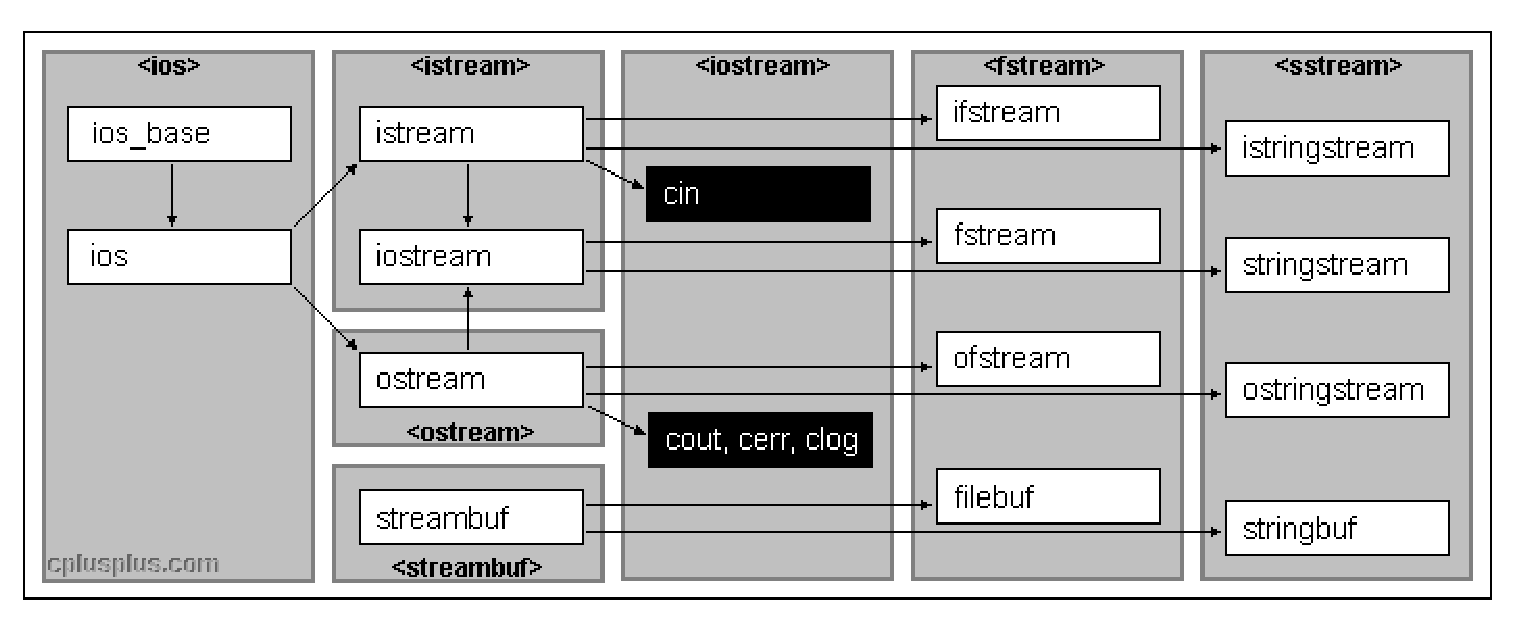
\includegraphics[height=5cm,
    angle=0]{./images/ios_hierarchy.eps}}
  \caption{}
  \label{fig:ios_hierarchy}
\end{figure}

The IO streams class hierarchy is given in Fig.\ref{fig:ios_hierarchy}.  An
important character of IO Stream is serial, we cannot make a random read or
random write to a string. Any built-in data types can be used with IO Streams'
APIs. To export values of user-defined data types, we need to override the {\bf
insertion operator} \verb!<<! to tell how to put objects into the stream, and
the {\bf extraction operator} \verb!>>! to tell how to read objects from the
stream. We can use 
\begin{verbatim}
#include <iostream>
using namespace std;


std::cout << "String to print out"
          << "another line to print out" 
          << std::endl;
\end{verbatim}


To format the parametric output, we use \verb!<iomanip>! (io manipulation). Each
manipulator receives one single argument, and returns one of the six unspecified
type T1 to T6
\footnote{\url{http://publib.boulder.ibm.com/infocenter/comphelp/v9v111/index.jsp?topic=/com.ibm.xlcpp9.aix.doc/standlib/header_iomanip.htm}}
\begin{verbatim}
namespace std {
  T1 resetiosflags(ios_base::fmtflags mask);
  T2 setiosflags(ios_base::fmtflags mask);
  T3 setbase(int base);
     template<class E>
  T4 setfill(E c);
  T5 setprecision(streamsize n);
  T6 setw(streamsize n);
}
\end{verbatim}
\begin{itemize}
  \item How many decimal points to print out after '0'
  \begin{verbatim}
  54.271123 and used setprecision(2) it would print out: 54.27 to the console.
  
  \end{verbatim}
  
  \item
  \begin{verbatim}
cout << setiosflags(ios::fixed) << setiosflags(ios::showpoint);  
  \end{verbatim}
\end{itemize}

\subsection{basic\_streambuf}
\label{sec:basic_streambuf}

\verb!basic_streambfu! is the abstract class, with a number of virtual functions
which are overridden to provide a uniform interface for reading/writing files, strings, etc.

\subsection{pubsetbuf()}

The only required behavior is that stream->pubsetbuf(0, 0) makes the file buffer
unbuffered which you almost certainly don't want. It doesn't make any guarantees
what happens if the arguments are non-null.
In particular, it doesn't guarantee that the buffer being used is the one being
passed! 

\subsection{streambuf}
\label{sec:streambuf}

All stream operations are buffered, with the base class streambuf is used behind
the scenes. It is provided with its own buffer, which size is an implementation
detail.

The stream buffer only affect the maximum number of bytes transferred to or from
the kernel with one syscall. Thus, the ideal buffer size doesn't depend on how
much data you transfer. What is does depend on is

\begin{verbatim}
The overhead cost of syscalls. 
        Higher overhead means you'll want to transfer more data in one go.

The overhead cost of buffer management. Probably larger for larger buffers, if anything.

CPU cache trashing effects. Will strongly favour smaller buffers.
\end{verbatim}
Since (1) works in favour of larger buffers while (2) and (3) work in favour of
smaller buffers, there will be a sweet spot somewhere.


Buffering:

If by default the buffer is very small, increasing the buffer size can definitely improve the performance:

    it reduces the number of HDD hits
    it reduces the number of system calls

Buffer can be set by accessing the underlying streambuf implementation.

\begin{verbatim}
char Buffer[N];

std::ifstream file("file.txt");

file.rdbuf()->pubsetbuf(Buffer, N);
// the pointer reader by rdbuf is guaranteed
// to be non-null after successful constructor
\end{verbatim}


\subsection{ios::rdbuf vs. fstream::rdbuf}

\begin{verbatim}
get (1)	
         streambuf* rdbuf() const;

set (2)	
         streambuf* rdbuf (streambuf* sb);
\end{verbatim}
sets the object pointed by sb as the stream buffer associated with the stream


\subsection{ofstream}

An ofstream by default opens its buffer in output mode only, and either way
you're only passing \verb!std::ios_base::out!, which means the buffer cannot be
read from.

\begin{verbatim}
To fix this you will need to switch to using an fstream and open it with
std::ios_base::in | std::ios_base::out | std::ios_base::binary

You will also need to seek to the start of the file before calling rdbufby
calling seekg(0, std::ios_base::beg).
\end{verbatim}

Use ofstream when textfile is for output only, ifstream for input only, fstream
for both input and output


\subsection{I/O with <istream>, <ostream> or <iostream>: peek(), getline(),
read(), readsome(), ignore()}
\label{sec:iostream}


If we don't care the physical input is a file, a buffer string, or a
console, then we just declare the variable as \verb!std::istream! for input and
\verb!std::ostream! for output. 

\verb!ostream! classes are just wrappers around I/O buffers, and provide
\verb!operator>>! formatting operators. The buffer is provided by an object
derived from \verb!basic_streambuf! (Sect.\ref{sec:basic_streambuf}), which you
can get and set using rdbuf().


There are 2 ways to connect to a file
\begin{verbatim}
// Option 1:
std::ifstream is ("test.txt", std::ifstream::binary);

// Option 2:
std::filebuf fb;
  if (fb.open ("test.txt",std::ios::in))
  {
    std::istream is(&fb);
    while (is)
      std::cout << char(is.get());
    fb.close();
  }
\end{verbatim}
then we can use proper methods to extract data in the form of single character,
a string or a block of data.

It has important functions that can be used in the children classes
\footnote{\url{http://www.cplusplus.com/reference/istream/istream/}}
\begin{itemize}
  \item Read but DON'T extract from the stream
  \begin{verbatim}
  int peek();
  \end{verbatim}
  Read the next character, without extracting. This is useful when you want to
  do parsing
  
  \item Extract character (using C++ string, i.e. you don't have to guess or
  specify the size of the pre-allocate buffer). However, if you read in a file,
  without specifying a \verb!delim! and there is no newline character in the
  file, then \verb!bad_alloc! error may occur.
  \begin{verbatim}
istream& std::getline (istream& is, string& str, char delim);
istream& std::getline (istream& is, string& str);
  \end{verbatim}
which extracts the content from \verb!is! and stores to \verb!str!, until a
delimiter is found (default=newline). NOTE: The delimiter, if found, is
extracted from the stream and is discarded, i.e. not store in \verb!str!.
  
  \item Extract characters (using C-style string):
  \begin{verbatim}
istream& std::istream::getline (char* s, streamsize n );
istream& std::istream::getline (char* s, streamsize n, char delim );
  \end{verbatim}
Extract characters and store them as C-style string \verb!s!, until 
\begin{itemize}
  \item a delimiter is read (default is newline \verb!'\n'!) or 
  \item $n-1$ characters has been read, and written \verb!s! (the $n$-th
  character is the \verb!null! character which is appended automatically)
  \item the end-of-file is reached, , if this occurs first, the \verb!eofbit!
  flag is set.
\end{itemize}
whichever first. A \verb!null! character (\verb!'\0'!) is automatically
appended, even if an empty string is returned.

If you want to be more flexible, you should use \verb!get()! method, which can
does what \verb!getline()! does, and more options: (1) extract a single
character, (2) put to the streambuffer.

  \item Read a block of data from the input (without checking the content nor
  appending NULL character at the end).
  \begin{verbatim}
  istream& istream::read (char* s, streamsize n);
  streamsize istream::readsome (char* s, streamsize n);
  \end{verbatim}
  extract up to $n$ characters, and store them into the array pointed by $s$.
  \verb!readsome()! is designed to work with some types of asynchronous sources
  that may eventually wait for more characters, as the function return as soon
  as the internal buffer is exhausted, i.e. avoiding potential delays.
  
  \item Extract from the input sequence, but discard them, until (whichever
  come first) $n$ characters or a delimiter is read. Default delimiter is EOF
  (end-of-file)
  \begin{verbatim}
  istream& ignore (streamsize n = 1, int delim = EOF);
  \end{verbatim}
  to focus on the delimiter, i.e. ignore as many as possible, we use 
  \begin{lstlisting}
  #include <limist>
  
  file.ignore(std::numeric_limits<std::streamsize>::max(), '}');
  \end{lstlisting}
  
  
  \item Return the number of characters read by the last {\it unformatted input
  operations} called by : \verb!get!, \verb!getline()!, \verb!read!, or
  \verb!readsome()!
  \begin{verbatim}
  streamsize gcount() const;
  \end{verbatim}
\end{itemize}

For output, similarly, we can use \verb!<ostream>!. And if we want to use the
stream for both input + output, we declare it as \verb!<iostream>!.

\subsection{File I/O with <fstream>, <ifstream>, <ofstream>}
\label{sec:std::fstream}

STL also incldue <fstream> which contains input and output stream classes.
\begin{enumerate}
  \item for input only: \verb!ifstream! class
  \item for output only: \verb!ofstream! class
  \item for input + output: \verb!fstream! class. There's an internal buffer
  object calls {\bf filebuf} that performs input/output  operations on the file
  it's associated with.   
\end{enumerate}
% NOTE: std::ifstream is INEFFICIENT compared to fread. The reason is that
% \verb!fread()! put the whole file into memory. So after \verb!fread()!,
% accessing the buffer is faster. 
Beside the standard way to open a file using \verb!.open()! member function, we
can also directly pass the filename when defining the ofstream object.
However, in C++98, the only way to open a file-stream by passing the filename is
to convert to C-style string.
\begin{verbatim}
	std::string filename("text.out");
#if defined(__CXX_EXPERIMENTAL_CXX0X__) || __cplusplus >= 201103L
	std::ofstream ofile(filename);
#else
	std::ofstream ofile(filename.c_str());
#endif	
\end{verbatim}

Another important thing is in C++11, \verb!ofstream! is movable. 

Example: \verb!ifstream:read()! is buffered, and we just tell how much data we
need to read in each time

{\small \begin{verbatim} 
void readFile()
{
    std::ifstream fin;
    fin.open("largefile.dat", ifstream::binary | ifstream::in);
    // in each of these small read methods, there are at least 1 fin.read()
    // call inside.
    readHeaderInfo(fin);
    readPreference(fin);
    readMainContent(fin);
    readVolumeData(fin);
    readTextureData(fin);
    fin.close();
}
\end{verbatim}}

TIPS: Use fread()/fwrite() for binary. maximize chunk size. Use fstreams for
ascii i/o. The best thing around is stream.getline() which saves you any string
ops if you want to extract data by newline (or any other delimiter). 

{\small \begin{verbatim} 
#include <iostream>
#include <fstream>
#include <streambuf>

ofstream ofs("file.txt" );
streambuf* original = cout.rdbuf();
cout.rdbuf( ofs.rdbuf() );  // cout now writes to the file

...

cout.rdbuf( original );  // MUST restore before quitting
\end{verbatim}}

\subsection{Temporay file}
\label{sec:temporary_file}

\verb!std::tmpfile! creates temporary binary file, open for update (``+wb''
mode). The filename is selected by the system, with guarantee that it's
different from any other existing files in the system.
\begin{verbatim}
FILE *pFile;
pFile = tmpfile ( void ); //the pointer to temporary file handle
 
 //work with pFile

fclose(pFile);
\end{verbatim}

To close and also delete the file, we use \verb!fclose(FILE*)!.  If the programs
terminate normally, whether the files are removed depends on the
library implementation.


We can use \verb!ostream!
\begin{verbatim}
char *tmpname = strdup("/tmp/tmpfileXXXXXX");
mkstemp(tmpname);
ofstream f(tmpname);
\end{verbatim}
NOTE: \verb!mkstemp()! can fail and return -1. So the code should catch that
case.

Here is another way
\begin{verbatim}
#include <stdlib.h>
#include <fstream>
#include <iostream>
#include <vector>

std::string open_temp(std::string path, std::ofstream& f) {
    path += "/XXXXXX";
    std::vector<char> dst_path(path.begin(), path.end());
    dst_path.push_back('\0');

    int fd = mkstemp(&dst_path[0]);
    if(fd != -1) {
        path.assign(dst_path.begin(), dst_path.end() - 1);
        f.open(path.c_str(), 
               std::ios_base::trunc | std::ios_base::out);
        close(fd);
    }
    return path;
}

int main() {
    std::ofstream logfile;
    open_temp("/tmp", logfile);
    if(logfile.is_open()) {
        logfile << "hello, dude" << std::endl;
    }
}
\end{verbatim}

References:
\begin{enumerate}
  \item \url{http://www.cplusplus.com/reference/cstdio/tmpfile/}
  
  \item
  \url{http://stackoverflow.com/questions/499636/how-to-create-a-stdofstream-to-a-temp-file}
\end{enumerate}

\subsection{Using user-defined set of routines}

We define a struct that keep the file-handle and file-name.
\begin{verbatim}
typedef struct {
   FILE* file;
   char* name;
} OBJECTFILE
\end{verbatim}

Then, we write a function to open a file \verb!object_fopen()!
\begin{verbatim}
OBJECTFILE file;
file = object_fopen(filename, "r")
\end{verbatim}
with
\begin{verbatim}
OBJECTFILE
object_fopen(const char* filename, char *mode)
{
  OBJECTFILE file;
  file.file = fopen(filename, mode);
  if (file.file == NULL) {
     char *msg;
     int msg_length;
     msg_length = strlen(filename) + 256;
     msg = (char*) Mallloc(msg_length);
     sprintf (msg, "%d: Error opening file=%s with mode %s from object_fopen",
        getRank(0), filename, mode);
     perror(msg);
     Free(msg);
  }
  
  filename = strdup(filename);
  return file;
}

void object_fclose(OBJECTFILE file)
{
  fclose(file.file);
  Free(file.name);
}   

char* object_read(OBJECTFILE file)
{  
}  
\end{verbatim}

\subsection{istringstream}

A stringstream is basically a string, but you can read/write data to it easily
using \verb!<<! and \verb!>>! operator, just like working with file or
\verb!std:cin!.

A stringstream works essentially like an input/output file stream. The
header file required is \verb!<sstream>!. To declare a stringstream, we do
\begin{verbatim}
#include <sstream>

stringstream ss;
\end{verbatim}

We can write to it or read from it using \verb!<<! or \verb!>>! operator
\begin{verbatim}
std::string myString;
char myChar;

ss << mychar ;
ss << myString;

int myInt;

ss >> myInt;
\end{verbatim}
Example:
\begin{lstlisting}
std::string s = "1 2 3"; // this is the original string
std::istringstream is(s); // this istringstream contains a copy of s
int i,j,k; // variables to write to
is >> i >> j >> k; // now i is 1, j is 2, and k is 3
\end{lstlisting}

To convert the entire stringstream to string
\begin{verbatim}
std::string str = ss.str();
\end{verbatim}


Other member functions from stream can be used with stringstream like
\verb!get!, \verb!getline()!, \verb!read!, \verb!write!, \verb!put()!


\section{Boost::Spirit.Karma (Output)}
\label{sec:boost_spirit_Karma}

Typically, \verb!printf, std::stream! formatting, or \verb!boost::format! have
been used for formatting output data. However, for complicated data structure,
it's hard to develop codes for writing data with proper format. A solution is
using \verb!Spirit.Karma! package from Boost::Spirit library. 


This is in opposite of Spirit::Qi which parse the input data from files into
internal data structure (Sect.\ref{sec:boost_spirit_Qi}).

\section{Boost::Spirit::Qi (Input)}
\label{sec:boost_spirit_Qi}

This is the parser library that we use to build recursive descent parsers
(Sect.\ref{sec:boost_spirit}).

Example:
\url{http://www.codeproject.com/Articles/8516/An-Introduction-to-the-Boost-Spirit-Parser-framewo}
We define a grammar class or struct, by inheriting \verb!boost::spirit::grammar!
class. In this class/struct, say \verb!MyGrammar!, we need to define a nested
struct called \verb!definition! (containing the language description that you
want to parse, i.e. a number of rules, ), and a member function call
\verb!start()! (returning the start rule).


\section{Boost::Spirit::Classic (Input)}
\label{sec:boost_spirit_classic}

This is considered depricated and we should use Boost::Spirit::Qi.

\url{http://www.codeproject.com/Articles/8516/An-Introduction-to-the-Boost-Spirit-Parser-framewo}

\url{http://www.codeproject.com/Articles/8522/Implementing-Semantic-Actions-in-the-Boost-Spirit}

{\small \begin{verbatim} 
struct MyGrammar :
    public boost::spirit::grammar<MyGrammar>
{
public:
    MyGrammar( CParser &parser );
    virtual ~MyGrammar();
    template <typename ScannerT>
    struct definition
    {
    public:
        definition( MyGrammar const &self )
        {
            integer =
                lexeme_d[ (+digit_p) ]
                ;
            factor =
                integer |
                vars |
                '(' >> expression >> ')' |
                ( '-' >> factor ) |
                ( '+' >> factor )
                ;
            term =
                factor >> *( ( '*' >> factor) | ( '/' >> factor ) )
                ;
            expression =
                term >> *( ( '+' >> term ) | ( '-' >> term ) )
                ;
            assignment =
                vars
                >> '=' >> expression
                ;
            var_decl =
                lexeme_d
                [
                    ( ( alpha_p >> *( alnum_p | '_' ) )
                    - vars )[vars.add]
                ]
                ;
            declaration =
                "int" >> var_decl >> *( ',' >> var_decl )
                ;
            baseExpression =
                str_p( "exit" )[*self.m_finishedProcessing] |
                str_p( "mod" ) >> integer |
                declaration |
                assignment |
                '?' >> expression
                ;
        }
        boost::spirit::symbols<int> vars;
        boost::spirit::rule<ScannerT> integer, factor, term,
            expression, assignment, var_decl, declaration,
            baseExpression;
        const boost::spirit::rule<ScannerT> &start() const { return baseExpression; }
    };
    friend struct definition;
private:
    Private::FinishedProcessing *m_finishedProcessing;
};
\end{verbatim}}

NOTE: The grammar is described using EBNF rules.
\begin{itemize}
  \item \verb!lexeme_d!: directive to tell the parser NOT to skip white spaces
  \item \verb!+digit_p!: directive to tell matching one or more numeric
  characters
  \item All the rules defined in the \verb!definition! struct, must also be
  defined in the class \verb!MyGrammar! of type
  \verb!boost::spirit::rule<ScannerT>!.
  \begin{verbatim}
        boost::spirit::rule<ScannerT> integer, factor, term,
            expression, assignment, var_decl, declaration,
            baseExpression;  
  \end{verbatim}
  \item The \verb!start()! function returns the entry point rule,
  i.e. baseExpression.
\end{itemize}

Now, after you have read-in the code in the form of a single string, we give it
to the parser.
\begin{verbatim}
//read-in input-file
//storing the content in 'line' string.

boost::spirit::parse_info<> info;
MyGrammar parser;
info = boost::spirit::parse( line.c_str(), parser, boost::spirit::space_p );
\end{verbatim}
NOTE: We can pass a string, or a pair of iterators for begin and end.



\section{Clang: parsing C/C++/Objective-C/Objective-C++ code}

{\bf Clang} is a powerful, free parser that can be used as a front-end for a
compiler \footnote{\url{http://clang.llvm.org/index.html}}. 

\section{Check file status}

We use the \verb!struct stat! structure which is a system struct that is
defined to store information about a given file. There are different field in
this structure. \url{http://codewiki.wikidot.com/c:struct-stat}

 {\small 
\begin{verbatim}
#include <iostream>
#include <sys/types.h>
#include <sys/stat.h>
#include <fcntl.h>
#include <string>
 using namespace std;

int main() {
     struct stat buf;
     std::string filename(``object.data'')
     stat(filename,&buf);

  cout << buf.st_dev << endl;     
 }
\end{verbatim}
}

Another way is to use \verb!filetest()!
\begin{verbatim}
#include <string>

std::string myfile("input.txt");

if (filetest(myfile.c_str(), S_IFREG) != 0) {
  cout << "File not exist";
}
\end{verbatim}

\section{Serialization (copying object's state)}
\label{sec:Serialization_C_C++}

The process to translate data structure or object state into the format that can
be stored (to harddrive), transfered (via network) and then resurrected later is
called {\bf serialization} (deflating, marshalling). This process is not trivial
if the object has extensive use of references. The reverse process, extracting
data structure from a series of bytes is called {\bf deserialization}
(inflating, unmarshalling).

A serialization need to provide at least 4 methods
\begin{enumerate}
  \item to write the object's data to a file or database
  \item to do RPC (remote-procedure call)
  \item to distribute the object
  \item to detect changes in time-varying data
\end{enumerate}
As we need to transfer the data across network, the implementation need to be
portable, i.e. users don't need to concern about byte-ordering, memory layout,
etc.

Serialization, however, breaks the opacity of abstract data type, i.e. you need
to expose private data member (i.e. data encapsulation).

\textcolor{red}{C/C++ do NOT provide direct support to serialization}. However, you can write
your own code for serialization. MFC (Microsoft Foundation Class) library also
provides serialization support. Another library is Boost.Serialization.

\subsection{Boost.Serialization}

The output file format can be: ASCII, XML, binary. The advantage of XML is
useful in debugging. Also, this format is propertary, so you cannot use it to
exchange data with application that doesn't use Boost.Serialization.

You have a simple class:
\begin{verbatim}
/////////////////////////////////////////////////////////////
// gps coordinate
//
// illustrates serialization for a simple type
//
class gps_position
{
private:
    int degrees;
    int minutes;
    float seconds;
public:
    gps_position(){};
    gps_position(int d, int m, float s) :
        degrees(d), minutes(m), seconds(s)
    {}
};
\end{verbatim}

The main concept of Boost.Serialization is an {\bf archive}, which is a sequence
of bytes representing serialized C++ objects. It means that an object can be
loaded into the archive to be serialize from them or to be loaded from it. 
To save the C++ object state to an archive which connect to a particular output
\begin{verbatim}
// Output archive as text stream.
// Even though it's not a stream, it can be used like a stream via << operator
#include <boost/archive/text_oarchive.hpp> 

// save the archive to standard output
boost::archive::text_oarchive oa(std::cout); 
\end{verbatim}


To restore object data from an archive which reads from file, we can use
\begin{verbatim}
#include <boost/archive/text_iarchive.hpp> 

//read from a text file
std::ofstream file("archiv.txt"); 
boost::archive::text_oarchive oa(file); 
\end{verbatim}


\subsubsection{If you can change the class definition}

You need to modify the class and a method name \verb!serialize()! must be
defined. This method is used for both serializing and restoring. The method
should never be called explicitly, and thus should be declared as private, and
the class \verb!boost::serialization::access! is declared as friend.

\begin{verbatim}
class gps_position
{
private:
    friend class boost::serialization::access;
    
    // When the class Archive corresponds to an output archive, the
    // & operator is defined similar to <<.  Likewise, when the class Archive
    // is a type of input archive the & operator is defined similar to >>.
    template<class Archive>
    void serialize(Archive & ar, const unsigned int version)
    {
        ar & degrees;
        ar & minutes;
        ar & seconds;
    }
...
}
\end{verbatim}

Then to save to text file and to restore the class data
\begin{verbatim}
#include <boost/archive/text_oarchive.hpp>
#include <boost/archive/text_iarchive.hpp>


int main() {
    // create and open a character archive for output
    std::ofstream ofs("filename");

    // create class instance
    const gps_position g(35, 59, 24.567f);

    // save data to archive
    {
        boost::archive::text_oarchive oa(ofs);
        // write class instance to archive
        oa << g;
    	// archive and stream closed when destructors are called
    }

    // ... some time later restore the class instance to its orginal state
    gps_position newg;
    {
        // create and open an archive for input
        std::ifstream ifs("filename");
        boost::archive::text_iarchive ia(ifs);
        // read class state from archive
        ia >> newg;
        // archive and stream closed when destructors are called
    }
    return 0;
}
\end{verbatim}

\subsubsection{If you can't (don't want to) change the class definition}

It means the class doesn't have to be derived from a specific class or implement
a specified member function.

You first need to make all data member public or make the class expose enough
information to reconstruct the class state.
\begin{verbatim}
class gps_position
{
public:
    int degrees;
    int minutes;
    float seconds;
    gps_position(){};
    gps_position(int d, int m, float s) :
        degrees(d), minutes(m), seconds(s)
    {}
};
\end{verbatim}

And then define a new member for Boost.Serialization
\begin{verbatim}
namespace boost {
namespace serialization {

template<class Archive>
void serialize(Archive & ar, gps_position & g, const unsigned int version)
{
//put any data member you want to output here
    ar & g.degrees;
    ar & g.minutes;
    ar & g.seconds;
}

} // namespace serialization
} // namespace boost
\end{verbatim}

Typically, we define two function \verb!save()! and \verb!load()!
\begin{verbatim}
void save() 
{ 
  boost::archive::text_oarchive oa(ss); 
  int i = 1; 
  oa << i; 
} 

void load() 
{ 
  boost::archive::text_iarchive ia(ss); 
  int i = 0; 
  ia >> i; 
  std::cout << i << std::endl; 
} 
\end{verbatim}

\subsubsection{Split load/save}

There are two cases: intrusive and non-intrusive approach:

\textcolor{red}{\bf Intrusive}: We need to include \verb!split_member.hpp!
header file, and then define two separate method \verb!save()! and \verb!load()!
to split the serialization into 2 separate functions.

\begin{verbatim}
#include <boost/serialization/split_member.hpp>
 
template<class Archive>
void save(Archive & ar, const unsigned int version) const
{
    // invoke serialization of the base class 
    ar << boost::serialization::base_object<const base_class_of_T>(*this);
    ar << member1;
    ar << member2;
    ar << member3;
}

template<class Archive>
void load(Archive & ar, const unsigned int version)
{
    // invoke serialization of the base class 
    ar >> boost::serialization::base_object<base_class_of_T>(*this);
    ar >> member1;
    ar >> member2;
    if(version > 0)
        ar >> member3;
}

template<class Archive>
void serialize(
    Archive & ar,
    const unsigned int file_version 
){
    boost::serialization::split_member(ar, *this, file_version);
}
\end{verbatim}

\textcolor{red}{\bf Non-intrusive}: 

We need to include \verb!split_free.hpp! file,
\begin{verbatim}
#include < boost/serialization/split_free.hpp>

namespace boost { namespace serialization {

template<class Archive>
inline void serialize(
    Archive & ar,
    my_class & t,
    const unsigned int file_version
){
    split_free(ar, t, file_version); 
}
}}

\end{verbatim}

\subsubsection{Data member as reference/pointer}

In the \verb!serialize()! member function we have
\begin{verbatim}
{
    // save/load class member variables
    ar & member1;
    ar & member2;
}
\end{verbatim}

If it's for a children class, we have
\begin{verbatim}
{
    // invoke serialization of the base class 
    ar & boost::serialization::base_object<base_class_of_T>(*this);
    // save/load class member variables
    ar & member1;
    ar & member2;
}
\end{verbatim}

If you have a data member which is a reference or a pointer, then how and where
the object being referred to are stored and how they are created, e.g.
\verb!member! data member in our case. REMEMBER: reference is a special kind of
pointer, so we serialize the reference as though it is a pointer 
\begin{verbatim}
class object;
class my_class {
private:
    friend class boost::serialization::access;
    int member1;
    object & member2;
    template<class Archive>
    void serialize(Archive &ar, const unsigned int file_version);
public:
    my_class(int m, object & o) :
        member1(m), 
        member2(o)
    {}
};
\end{verbatim}

Then we define an override
\begin{verbatim}
namespace boost { namespace serialization {
template<class Archive>
inline void save_construct_data(
    Archive & ar, const my_class * t, const unsigned int file_version
){
    // save data required to construct instance
    ar << t.member1;
    // serialize reference to object as a pointer
    ar << & t.member2;
}

template<class Archive>
inline void load_construct_data(
    Archive & ar, my_class * t, const unsigned int file_version
){
    // retrieve data from archive required to construct new instance
    int m;
    ar >> m;
    // create and load data through pointer to object
    // tracking handles issues of duplicates.
    object * optr;
    ar >> optr;
    // invoke inplace constructor to initialize instance of my_class
    ::new(t)my_class(m, *optr);
}
}} // namespace ...
\end{verbatim}


\subsubsection{Class versioning}

If we change the class definition, we can use version to determine how to load
the data. When we serialize a class, we have the option to pass the version
information to it.

When it is loaded from the archive, the version number is passed as an argument
to the loading function, we can check using \verb!file_version!
\begin{verbatim}
{
    // invoke serialization of the base class 
    ar & boost::serialization::base_object<base_class_of_T>(*this);
    // save/load class member variables
    ar & member1;
    ar & member2;
    // if its a recent version of the class
    if(1 < file_version)
        // save load recently added class members
        ar & member3;
}
\end{verbatim}

\subsubsection{Using XML}

\begin{verbatim}
boost::archive::xml_oarchive xmlArchive(oStringStream);

xmlArchive.register_type(static_cast<BaseMessage *>(NULL));
xmlArchive.register_type(static_cast<IncomingTradeMessage *>(NULL));
xmlArchive.register_type(static_cast<InternalRequestInfo *>(NULL));
xmlArchive.register_type(static_cast<InternalTradeTransInfo *>(NULL));

const BaseMessage* myMessage =message;

xmlArchive << make_nvp("Message", myMessage);
\end{verbatim}

\subsubsection{Inheritance}

How Boost.Serialization know the class of the object it serializes has a parent,
or even what that parent is.

\begin{lstlisting}
class MyParent {
public:
	
private:
	int ID;
    friend class boost::serialization::access;
    
	template<class Archive> void serialize(Archive& ar,
       const unsigned int version) 
    {
		ar & BOOST_SERIALIZATION_NVP(ID);
	}	
\end{lstlisting}

\begin{lstlisting}
class ChildClass :: MyParent 
{
public:

private:
	friend class boost::serialization::access;
    template<class Archive> void serialize(Archive& ar,
        const unsigned int version) {
          
           /// what should be here???
           /// check below
    }
}
\end{lstlisting}


To serialize the childen class, we need to tell the compiler 
what the object's parent is and provide a reference to it, you can put this line
at the beginning or the end of the \verb!serialize()! member function of the
children class, depening on how you want to structure the output
\begin{verbatim}
ar & boost::serialization::make_nvp("MyParent",
     boost::serialization::base_object<MyParent>(*this))
\end{verbatim}
\url{http://stuartjames.info/Journal/boost-serialization-for-inherited-objects.aspx}

Another option: the children class need have access to
\verb!boost::serialization::base_object()! function inside the
\verb!serialize()! method.
\begin{verbatim}
#include <fstream>
#include <boost/serialization/export.hpp>
#include <boost/archive/text_oarchive.hpp>

class Foo {
    friend class boost::serialization::access;

    template<class Archive>
    void serialize(Archive & ar, const unsigned int version)
    {
        ar & dummy1;
    }

    int dummy1;

public:
    virtual ~Foo() {}
};


class Bar : public Foo {
    friend class boost::serialization::access;

    template<class Archive>
    void serialize(Archive & ar, const unsigned int version)
    {
        // serialize base class information
        ar & boost::serialization::base_object<Foo>(*this);
        ar & dummy2;
    }

    int dummy2;
};

BOOST_CLASS_EXPORT_GUID(Foo, "Foo")
BOOST_CLASS_EXPORT_GUID(Bar, "Bar")

int main(int argc, char *argv[]) {
    std::ofstream ofs("filename");
    boost::archive::text_oarchive oa(ofs);
    Foo *f = new Bar;
    oa << f;

    return 0;
}
\end{verbatim}

\subsection{ACCU}

\url{http://accu.org/index.php/journals/486}


\section{UTF-16 file data}


\subsection{Library: ICU}
\label{sec:ICU}


International Components for Unicode (ICU) provides a cross-platform,
Unicode-based globalization for handling text data in any formats
\footnote{\url{http://site.icu-project.org/home}}.

\begin{itemize}
  \item convert text data to/from Unicode and nearly any other character sets
  \item compare string: based on Unicode Collation Algorithm plus
  locale-specific comparison rules.
  
  \item format string that represents numbers, date, times, currency according
  to a chosen locale.
  \item regular expression: able to handling text left-to-right (English) or
  light-to-left (Arabic, Hebrew) data
  \item text boundaries: 
\end{itemize}

\begin{mdframed}
Why not using ICU?
\begin{itemize}
  \item APIs do not follow modern C++ design, and do not work well with
  newer versions of standard C++ library
  (Sect.\ref{sec:standard-C++-library})
  
  \item UTF-16 oriented. No support for narrow encoding (e.g. ISO 8859)
  
  \item Message translation tool is far from perfect, which can be done with
  GNU \verb!Gettext! model in Boost.Locale (Sect.\ref{sec:Boost.Locale})
  
\end{itemize}

Why using ICU?
\begin{itemize}
  \item one of the best localization/Unicode libraries available
  \item 
\end{itemize}
\end{mdframed}


Compile and install the library before using:
\footnote{\url{http://stuf.ro/reading-a-utf-8-file-in-c-with-icu}}
\begin{verbatim}
// we use -E -H to preserve the environment variables in 'sudo' mode
./configure --enable-static --prefix=/usr && make && sudo -E -H make install

/* statically linking (need to use g++ even for C-code) */
g++ main.c -o main.o -static -lsicuio -lsicui18n -lsicuuc -lsicudata

/* dynamically linking */
gcc main.c -o main.o `icu-config --ld-flags --ld-flags-icuio`
\end{verbatim}


The new data type is \verb!UChar*!, and string operating functions is the same
as C-library except with a prefix \verb!u_!, e.g. \verb!u_printf, u_fclose!. To
allocate and free the string, the function doesn't change, \verb!free()!.
\begin{verbatim}
UChar* str = (UChar*) malloc(sizeof(UChar) * (fsize + 1));
\end{verbatim}

The file object is \verb!UFILE!, with \verb!u_fopen(), u_fclose()! functions.

Example:
\begin{Verbatim}
#include <stdio.h>
#include <stdlib.h>

#include "unicode/ustdio.h"
#include "unicode/uchar.h"

/**
 * Reads a UTF-8 file and returns an UChar array containing the string read.
 *
 * @param filename the path to the file to be read
 * @param size pointer to a variable in which to store the UTF-8 string length
 *
 * @return UTF-8 string (dynamically allocated; must be freed after usage)
 */
UChar* read_utf8_file(const char* filename, long* size) {
    /* open a UTF-8 file for reading */
    UFILE* f = u_fopen(filename, "r", NULL, "UTF-8");

    /* get the file size */
    long fsize;
    fseek(u_fgetfile(f), 0, SEEK_END);
    fsize = ftell(u_fgetfile(f));
    u_frewind(f);

    /* allocate enough memory to store the whole string plus termination */
    UChar* str = (UChar*) malloc(sizeof(UChar) * (fsize + 1));

    /* read the string into the allocated space */
    for ((*size) = 0; !u_feof(f); ++(*size)) {
        str[*size] = u_fgetc(f);
    }

    /* add NULL termination */
    str[*size] = 0;

    /* close the file resource */
    u_fclose(f);

    return str;
}

int main() {
    /* read the string and its size */
    long size;
    UChar* str = read_utf8_file("utf8_test.txt", &size);

    /* print the string size */
    printf("String size: %ld\n\n", size);

    /* print the UTF-8 string */
    UFILE* u_stdout = u_finit(stdout, NULL, NULL);
    u_fprintf(u_stdout, "%S\n", str);
    u_fclose(u_stdout);

    /* free the allocated string */
    free(str);

    return 0;
}
\end{Verbatim}
\section{UTF-8 file data}

If the file is encoded in UTF-8.

\subsection{Microsoft VC++}
\label{sec:wide-character_VC++}

In Microsoft Visual C++ 2005, we can use \verb!fgets()! to decode UTF-8 encoded
file when we create the stream using an extension \verb!ccs=encoding! to open file using
FILE object (Sect.\ref{sec:C-stream-IO}). However, in Visual C++ 2005, this only
work for opening only, not for writing. Other encoded types are also supported
\begin{verbatim}
"ccs=UNICODE" => UTF-16 (Big endian)
"ccs=UTF-8" => UTF-8
"ccs=UTF-16LE" => UTFS-16LE (Little endian) 
"ccs=ANSI" => ANSI (default encoding of the OS)
\end{verbatim}

%wchar_t* unicode_text = L"こんにちは";
Example: reading in
\begin{verbatim}
wchar_t* unicode_text[100];
FILE* f = fopen("C:\\test.txt", "w,ccs=UTF-8");
// fwprintf(f, L"%s\n", unicode_text);
fgets(f, unicode_text);
fclose(f);
\end{verbatim}


For reading in, if you know the locale, you can set with \verb!locale()!
\begin{verbatim}

wchar_t buffer[1000];
FILE* f = fopen("C:\\test.txt", "r");
fgetws(buffer, 1000, f);
fclose(f);

//MessageBoxW(0, buffer, 0, 0);
wprintf (L"% s ", buffer)
\end{verbatim}
Use \verb!fgetws()! to read-in wide-character string.

\subsection{Boost.Locale}
\label{sec:Boost.Locale}

\url{http://www.boost.org/doc/libs/1_55_0/libs/locale/doc/html/index.html}

Boost.Locale connect C++ locale framework, isostreams, and the powerful ICU
library (Sect.\ref{sec:ICU}). Also, Boost.Locale provide non-ICU localization
support.

As ICU is huge (half a million lines of well-tested code), Boost.Locale only
wraps ICU with a modern C++ interface. The entire ICU is hidden behind opaque
pointer and users have no access to it.

% \include{Files}
% \include{DateTime}
% %%
%% GenerateData.tex
%% Login : <hoang-trong@hoang-trong-laptop>
%% Started on  Thu Oct  1 12:07:44 2009 Hoang-Trong Minh Tuan
%% $Id$
%% 
%% Copyright (C) 2009 Hoang-Trong Minh Tuan
%%

\chapter{Generate Data}
\label{chap:generate-data}

The Mersenne Twister algorithm (Sect.\ref{sec:PRNG_Mersenne-Tiwstter}) is
available in C++ language since C++11 standard.

In early version of C++, the header file \verb!cstdlib! (C++) or \verb!stdlib.h! provides function for PRNGs
\begin{itemize}
  \item \verb!RAND_MAX! - a macro that extends to an integer constant
  
  \item \verb!std::rand()! - a function returning a PRN in the interval \verb!(0, RAND_MAX)!
  
  \item \verb!std:srand()! - pass a seed to the PRNG used by \verb!std:rand()!
\end{itemize}
The algorithms underlying even this minimal support have typically been unspecified, and
hence their use has historically been nonportable. 
\url{http://www.open-std.org/jtc1/sc22/wg21/docs/papers/2013/n3551.pdf}

\section{C++11: <random>}
\label{sec:C++11_random}


C++11 provides a new header file for PRNG 
\begin{lstlisting}
#include <random>
\end{lstlisting}
In C++11, there is a clear difference between the {\bf engine} and the {\bf distribution}.
\begin{itemize}
  \item the {\bf engine}'s role is to return unpredictable (random) bits, ensuring the probability (or likelihood) of obtaining
  a 0 bit is always the same as that of obtaining a 1 bit.
  
The purpose of the engine is to serve as a source of randomness. The sequence would be in uniform distribution.  
  
  \item the {\bf distribution}'s role is to convert the bits in uniformly distributed sequence into the number of proper distribution.
\end{itemize}
The terms engine and distribution are applied not only to types meeting certain requirements specified in the C++11
standard, but also to objects of such types.

\subsection{Create an engine}

The engine controls the sequence of PRNG.
The two engines initialized of the same state always return the same two sequence of PRNGs.
Such replication can be very useful while debugging a program or reproducing research, for example.

To escape replication, the engine's seed must vary from run to run
\begin{itemize}
  \item traditional approach: use system clock, \verb!time(0)!, or access to system-specific resource, \verb!/dev/urandom!
  
  \item C++11 approach: use \verb!std::random_device! as the seed
\end{itemize}

There are two ways to initialize an engine: implicit vs. explicit (which we can
also provide a seed). The type of the seed must be the same as (or convertible
to) the type of the values produced by the engine.


\begin{verbatim}
#include <random>

std::default_random_engine e1; // implicitly default-initialized
static std::default_random_engine e{};  // explicit default-initialized

std::default_random_engine e3{13607};

std::random_device rdev{};
std::default_random_engine e{rdev()};
\end{verbatim}

An engine's state can be reset any time after it has been initialized
\begin{lstlisting}
void f( std::default_random_engine & e4, std::random_device & rd )
{
  e4.seed(13607); // e4 state now as if initialized by 13607

  e4.seed(); // now as if default-initialized

  e4.seed(rd()); // now as if initialized via the device-obtained seed
}
\end{lstlisting}

List of all engines:
\begin{itemize}
  \item light-weight use:   \verb!std::default_random_engine!
  \item knowledge use: 
\begin{itemize}
  
  \item \verb!std::mt19937!, \verb!std::mt19947_64!: mersenne twister
  
  \item \verb!minstd_rand0, minstd_rand!: linear congruential engines
  
  \item \verb!ranlux24_base, ranlux48_base!: subtract with carry engine
  
   \item \verb!ranlux24, ranlux48!: discard block engine
   \item \verb!knuth_b! : shuffle order engine
\end{itemize}
  \item for expert (researcher): the following templates can be configured via template parameters 

\begin{verbatim}
linear_congruential_engine 
discard_block_engine
mersenne_twister_engine 
independent_bits_engine
subtract_with_carry_engine 
shuffle_order_engine

\end{verbatim}
\end{itemize}

\subsection{Create a distribution}

{\bf Uniform distribution}:
\begin{lstlisting}
int lbound = 1;
int ubound = 6;
static std::uniform_int_distribution<int> d{lbound, ubound};
\end{lstlisting}

\url{http://www.open-std.org/jtc1/sc22/wg21/docs/papers/2013/n3551.pdf}

\subsection{Return a PRN based on the created distribution and engine}

We pass the engine to the distribution.

\begin{lstlisting}
#include <random>
int roll_a_fair_die( )
{
  static std::default_random_engine e{};
  static std::uniform_int_distribution<int> d{1, 6};
  return d(e);
}
\end{lstlisting}




\section{File with given sizes}

Create file at a given size, containing only zeros
\begin{verbatim}
dd if=/dev/zero bs=1024 count=<number-of-kilobytes> > myfile
\end{verbatim}

%%% Local Variables: 
%%% mode: latex
%%% TeX-master: "fortran_manual"
%%% End: 

% \include{F2003-2008}
% 
\part{Benchmark}
\import*{../Fortran_manual/}{Datetime.tex}
% \chapter{Data type: Date time}
% \label{chap:date_time}
% 


% \section{Date-time}
% \label{sec:date_time}

\section{Year 2038 problem}

Due to the complication of using date time (local vs. GMT time, Year 2038 bug
problems), you are suggested to use 64-bit data type (i.e. \verb!long long! in
GNU C or POSIX/SUS-systems), and use GMT-time all the times. Suggestions
\begin{enumerate}
  \item  Using local time,
even though easier for a human to know the time of the event in referenced to
the time of current geographical area of the user, it's hard to compare with
other time due to the complexity of converting them to the same
references due to daylight saving available in some countries and the saving
varies from countries to countries, as well as the GMT offset complexities.

  \item When you use more than 2 libraries, make sure the data types are of the
same size. This will allows the code to be recompiled easily
  
\end{enumerate}

Example: after it passes the largest number, the 32-bit data
is interepted as year 1901 \url{http://en.wikipedia.org/wiki/Year_2038_problem}
\begin{verbatim}
Hexa (32-bit): 0x7FFFFFFF
Binary :  01111111  11111111  11111111  11111111  
Decimal: 2147483647
Date (interpreted)   : 2038-01-19 03:14:07 (UTC)
Date (true)  : 2038-01-19 03:14:07 (UTC)

//after it pass the maximum value --> it becomes negative
Binary :  10000000  00000000  00000000  00000000
Decimal: -2147483648
Date (interpreted)   : 1901-12-13 20:45:52 (UTC)
Date (true)  : 2038-01-19 03:14:08 (UTC)
\end{verbatim}

This is known as {\bf Unix Millenium bug} which is a serious problems in
embedded systems which still use 8-bit, 16-bit or 32-bit microprocessors.
Embedded systems are being used every where: mirowave ovens, gas stations, car
fuel injection computers, radios, \ldots


There is no universal solution to the Year 2038 problem. A solution is to use
struct \verb!tm! (Sect.\ref{sec:struct_tm}) or using the new 64-bit definition
for \verb!time_t!.
\begin{verbatim}
  // in Cygwin
#typedef unsigned long long time_t


// /usr/include/bits/types.h
typedef long int __time_t;
typedef __time_t time_t;
\end{verbatim}


Another options is to write your own function:
\url{http://www.2038bug.com/developers.html}


\section{struct tm}
\label{sec:struct_tm}

The header file is \verb!<time.h>! (in C) or \verb!<ctime>! (in C++).

In C90 (C++98), the struct \verb!tm! has 9 members, in any order
\begin{verbatim}
int tm_sec; //second (0..61*) [FIXED 0..60 in C99/C++11]
int tm_min; // minutes (0..59)
int tm_hour; //hours since midnight (0..23)
int tm_mday; //day of the month (1..31)
int tm_mon;  //month since Jan (0..11)
int tm_year; // year since 1900
int tm_wday; // day since Sunday (0..6)
int tm_yday; // days since Jan-1 (0..365)
int tm_isdst; //daylight saving flag (0 or 1)
\end{verbatim}
NOTE: \verb!tm_sec! is generally 0..59. However, the extra value is to
accommodate for leap seconds in certain years. [NOTE: {\bf leap seconds} is
one-second adjustment applied to UTC in order to keep the ]

\verb!tm! struct is being used in some functions
\begin{verbatim}
time_t mktime(struct tm*	)		// convert from tm to time_t (local time)
struct tm localtime( )  // return current local time (left or right of GMT)
                        // and inclusive any daylight-saving offsets.
struct tm gmtime( )    // return current GMT-time
char* asctime(const struct tm*	)  //convert from struct tm to string 
\end{verbatim}
The string returned by \verb!asctime()! is in the same format as \verb!ctime()!
function, which uses the information from these fields: 
\begin{verbatim}
tm_wday
tm_mon
tm_mday
tm_hour
tm_min
tm_sec
1900+tm_year
\end{verbatim}

Example:
\begin{verbatim}
  static const char wday_name[][4] = {
    "Sun", "Mon", "Tue", "Wed", "Thu", "Fri", "Sat"
  };
  static const char mon_name[][4] = {
    "Jan", "Feb", "Mar", "Apr", "May", "Jun",
    "Jul", "Aug", "Sep", "Oct", "Nov", "Dec"
  };
  static char result[26];
  sprintf(result, "%.3s %.3s%3d %.2d:%.2d:%.2d %d\n",
    wday_name[timeptr->tm_wday],
    mon_name[timeptr->tm_mon],
    timeptr->tm_mday, timeptr->tm_hour,
    timeptr->tm_min, timeptr->tm_sec,
    1900 + timeptr->tm_year);
  return result;
\end{verbatim} 


\section{time\_t}
\label{sec:time_t}

ISO C define \verb!time_t! as an arithmetic type, but doens't specify any
particular type, or the range, resolution or encoding of it. Also, it doesn't
specify the meaning of arithmetic operations on the data of this type. So, it's
pretty much implementation dependent. The header file is \verb!<time.h>! (in C)
or \verb!<ctime>! (in C++). To check how \verb!time_t! is defined, we write a
simple code and compile like this
\begin{verbatim}
#include <time.h>

int main(int argc, char** argv)
{
        time_t test;
        return 0;
}
\end{verbatim}
and compile
\begin{verbatim}
gcc -E test.c | grep 'time_t'
\end{verbatim}

The function that deals with \verb!time_t! data treat the value as \verb!local!
time. The value of using \verb!local! time, which can changes depending where
the machine is running on the globe (i.e. GMT time or Greenwich Mean Time or UTC
- Coordinated Universal Time). So, if two machines talk to each other, the
current time between them, using this function, can be a few hours difference.
To make sure it's the same, they should be referenced to the same place, i.e.
UTC time. This can be done using \verb!gmtime()! function.

\begin{enumerate}
  \item \verb!time()!: return the current calendar time (in seconds) compared to
  the intial time (as described below). 
  
\begin{verbatim}
time_t time(time_t *);
\end{verbatim}  
If the argument is not a NULL value, then the current calendar time is returned
to this value as well.

   \item \verb!ctime()!: convert the time (in local reference time) to string.

\begin{verbatim}
char* ctime(const time_t * timer); 
\end{verbatim}
This is equivalent to \verb!asctime(localtime(timer)!
   
The C-string is in the format \verb!Www Mmm dd hh:mm:ss yyyy!, followed by a
character \verb!'\n'!, and terminated by a NULL-character.
\begin{verbatim}
Wwww = weekday
Mmm  = month (in letters)
dd   = day of the month
hh:mm:ss = time 
yyyy = year
\end{verbatim}

   \item \verb!gmtime():!
\end{enumerate}

{\bf UNIX and POSIX-compliant system}: 
\begin{verbatim}
   // 32-bit or 64-bit wide depending which CPU architecture
   //                       and operating system
#typedef signed integer time_t
\end{verbatim}
The value of this type tells the number of seconds since the start of the Unix
epoch, i.e. {\it midnight UTC of January 1, 1970} (not counting leap seconds). 

If it's a 32-bit value, then consider the largest value and it causes Year 2038
problem
\begin{verbatim}
#include <stdio.h> /* printf */
#include <time.h>  /* time_t */

time_t biggest_in_seconds = 0x7FFFFFFF;

printf("biggest time in the future = %s ", ctime(&biggest));
\end{verbatim}

\section{Convert to string}
\label{sec:datetime_to_string}

We can use \verb!ctime(), ctime_r()! 

We can use \verb!asctime()!

We can use \verb!strftime()! function, which interprets the data in
\verb!timptr! to the string pointed by \verb!s! using the format given by
\verb!format!. The maximum characters (including the NULL-character) of the
string pointed by \verb!s! is given in \verb!maxsizes!.
\begin{verbatim}
#include <time.h>

size_t strftime(char *s, size_t maxsize, const char *format,
    const struct tm *timptr);
\end{verbatim}
The function returns the total number of characters (not including the
NULL-character) copied to \verb!s! if the total length copied is less than
\verb!maxsizes! (i.e. successful). Otherwise, it returns 0 (which can be used
to detect error) and the contents of the string pointed by \verb!s! is
indeterminate.

\url{http://pubs.opengroup.org/onlinepubs/007908799/xsh/strftime.html}


Example:
\begin{Verbatim}
#include <stdio.h>      /* puts */
#include <time.h>       /* time_t, struct tm, time, localtime, strftime */

int main ()
{
  time_t rawtime;
  struct tm * timeinfo;
  char buffer [80];

  time (&rawtime);
  timeinfo = localtime (&rawtime);

  strftime (buffer,80,"Now it's %I:%M%p.",timeinfo);
  puts (buffer);

\end{Verbatim}


\section{Thread-safe functions}

MinGW provides both \verb!*_r()! and \verb!*_s()! functions. The \verb!*_r()!
are the re-entrant (thread-safe) versions

\subsection{POSIX}

Added to SUS (Single Unix Specification) version 2: \verb!gmtime_r()!,
\verb!asctime_r()!, \verb!ctime_r()!, and \verb!localtime_r()!.

Example: The function \verb!gmtime()! is not thread-safe as it
use a pointer to an internal object of type \verb!struct tm!. A thread-safe
version is \verb!gmtime_r()! (on standard POSIX-compliant system) or
\verb!gmtime_s()! (on Windows system). Using these thread-safe are non-portable
\begin{verbatim}
  // the order of the arguments are different
  
  // return a pointer pointing to the value the same as the second argument
  // or return a NULL pointer if failed
struct tm* gmtime_r(const time_t*, struct tm*)

  // return 0 (successful) 
  // or errno_t value if failed
int gmtime_s(struct tm*, const time_t*)
\end{verbatim}

\subsection{Windows}

These functions are added to Windows' Secure CRT (Secure C run-time):
\verb!gmtime_s()!, \verb!asctime_s()!, \verb!ctime_s()!, and
\verb!localtime_s()!. 

NOTE: Thread-safety is not an issue with \verb!gmtime()! and \verb!localtime()!
in Windows, and the output is allocated per thread. Here, the two new functions
added to do Secure CRT's parameter validation (e.g. checking if the parameter
are NULL to evoke error handling or not).


\section{<chrono> (C++11)}
\label{sec:chrono-header-file}

Since C+=11, the header file \verb!<chrono>! has been added and contains
elements to deal with time.
\begin{enumerate}
  \item measure duration, i.e. time spans
  
  \item a specific time point
  
  \item relate time point to real physical time
\end{enumerate}

This is adopted from Boost::Chrono library (Sect.\ref{sec:Boost.Chrono})

\url{http://www.cplusplus.com/reference/chrono/}

To convert from
\begin{verbatim}
std::chrono::system_clock::time_point
\end{verbatim}
to \verb!time_t!, we use

\begin{lstlisting}
time_t  data = std::chrono::system_clock::to_time_t(...)
\end{lstlisting}

Finally, use the normal C function \verb!ctime()! or strftime to format it.

\begin{verbatim}
std::chrono::system_clock::time_point tp = std::chrono::system_clock::now();

std::time_t time = std::chrono::system_clock::to_time_t(tp);
std::tm timetm = *std::localtime(&time);
std::cout << "output : " << std::put_time(&timetm, "%c %Z") << "+"
          << std::chrono::duration_cast<std::chrono::milliseconds>(tp.time_since_epoch()).count() % 1000 << std::endl;
          
\end{verbatim}

\url{http://www.cplusplus.com/reference/ctime/strftime/} 
\chapter{Benchmark}


\section{Linux shell ``time": whole program}


\begin{lstlisting}
$ time ./a.out
\end{lstlisting}


\section{clock(): <time.h>}
\label{sec:clock()_C}


\verb!clock()! is standard in C language, whichmeasures the CPU time, and the
return a floating number of type \verb!clock_t!, as the number of clocks
ellapsed.
The number of clocks per second is architecture-specific, and can be checked via
\verb!CLOCKS_PER_SEC! constant.

\begin{lstlisting}
#include <time.h>

int main()
{
    clock_t tic = clock();

    my_expensive_function_which_can_spawn_threads();

    clock_t toc = clock();

    printf("Elapsed: %f seconds\n", (double)(toc - tic) / CLOCKS_PER_SEC);

    return 0;
}
\end{lstlisting}


\section{gettimeofday(): <sys/time.h>}	


\section{C++ Boost library: Chrono}

Sect.\ref{sec:Boost.Chrono}


\section{C++11: }


\part{Build \& Compile}
\chapter{Compile}
\label{chap:compiler}


The C source code files can be compiled into different targets (static lib,
shared lib, executable file), for different platform (32-bit, 64-bit, ARM).
In general, compilation goes through 2 steps:
{\bf compiling} and {\bf linking}. 

First, the compiler convert the source code (the .cpp file) to object file
(*.o). At this time, the code may have reference to non-completed types, i.e.
those whose declaration are available via header files; but whose definition are
not available yet.
In the first step, the compiler takes a {\bf compilation unit}
(Sect.\ref{sec:compilation-unit}).

At linkage stage, then, the linker takes all the object files, together with
statistically-linked libraries, to create a binary program.

It's important to know how to best organize the code (Sect.\ref{sec:modules-in-C++}).

Different IDE tools allows us to do this easily. Chap.\ref{chap:Visual_C++}
describes how to compile C/C++ projects using Visual Studio.
Chap.\ref{chap:compile_Csharp} how to use Visual Studio for C\# language. To
compile your code into a library, you should also read Chap.\ref{chap:library}.

\section{Manage complexity of a C/C++ project}
\label{sec:modules-in-C++}

C and C++ programs normally take the form of a collection of separately compiled
modules.
As a big project is developed, an new executable can be built rapidly if only
the changed modules need to be recompiled.

\textcolor{red}{\bf What is a module in C/C++?}:
In C++, the contents of a module consist of structure type (struct)
declarations, class declarations, global variables, and functions.
The functions themselves are normally defined in a source file (a “cpp” file).

Each source (.cpp) file has a header file (a “.h” file) associated with it
that provides the declarations needed by other modules to make use of this
module.

The idea is that other modules can access the functionality in module X simply
by \verb!#include!'ing the “X.h” header file, and the linker will do the rest.

The code in X.cpp needs to be compiled only the first time or if it is changed;
the rest of the time, the linker will link X’s code into the final executable
without needing to recompile it, which enables the Unix make utility and IDEs to
work very efficiently.

Usually, the main module (i.e. the one with \verb!main()! function) does not
have a header file, since it normally uses functionality in the other modules,
rather than providing functionality to them.

IMPORTANT: compilers and linkers need help in enforcing the One Definition Rule
(Sect.\ref{sec:one-definition-rule}).

\textcolor{red}{Well-designed header file to reduce the coupling}:

Reduce the amount of “coupling” between components by minimizing the number of
header files that a module’s header file itself \verb!#include!s. On very large
projects (where C++ is often used), minimizing coupling can make a huge differ-
ence in “build time” as well as simplifying the code organization and debugging.

\subsection{Design a good module}
\label{sec:module-in-C++-good-design}
\label{sec:compilation-unit}

Each module with its .h and .cpp file should correspond to a clear piece of
functionality.
The Standard Library modules <cmath> and <string> are good examples of clearly
distinct modules.
{\it Don’t force together into a module things that will be used or maintained
separately, and don’t separate things that will always be used and maintained
together.}


Always use “include guards” in a header file. Choose a guard symbol based on the
header file name, since these symbols are easy to think up and the header file
names are almost always unique in a project.
For example “Geometry_base.h” would start with:
\begin{verbatim}
#ifndef GEOMETRY_BASE_H
#define GEOMETRY_BASE_H
\end{verbatim}
and end with:
\begin{verbatim}
#endif
\end{verbatim}
 
 
If module A needs to use module X’s functionality, it should always 
\begin{verbatim}
#include “X.h”
\end{verbatim}	
, and never contain hard-coded decla- rations for structs, classes,
globals, or functions that appear in module X.

The reason is that: If module X is changed, but you forget to change the
hard-coded declarations in module A, module A could easily fail with subtle
run-time errors that won’t be detected by either the com- piler or linker.
  

\textcolor{red}{RULE 6}:
Set up global variables for a module with an extern declaration in the header
file, and a defining declaration in the .cpp file.
\begin{verbatim}
// in header file
// place an extern declaration in the .h 
// it means that any files included this header file
//  can use 'g_number_of_entities' (without asking where it is)
//  it's location/definition will be provided at linkage time
//  by linking the object file (compiled form the .C file containing the unique definition
//  of 'g_number_of_entities' (below)

extern int g_number_of_entities;
\end{verbatim}
and in source file
(the .cpp file for the module) must include this same .h file, 
and near the beginning of the file, a defining declaration should appear.
This declaration both defines and initializes the global variables

\begin{verbatim}
// the source file
// where unique-definition occurs

// static/global variables are initialized to zero by default; but initializing
// explicitly to zero is customary because it marks this declaration as the
// defining declaration, meaning that this is the unique point of definition.

int g_number_of_entities = 0;
\end{verbatim}

NOTE: different C compilers and linkers will allow other ways of setting up
global variables, but this is the accepted C++ method for defining global
variables and it also works for C to ensure that the global variables obey the
One Definition Rule.
 
\url{http://umich.edu/~eecs381/handouts/CppHeaderFileGuidelines.pdf}



\section{Translation units}

\label{sec:translation-unit}


A {\bf translation unit} is not "a header and a source file". It could include a
thousand header files (and a thousand source files too).
A translation unit is typically a pre-processed source file (i.e a source file
with all the contents of all header files)

A translation unit is simply what is commonly known as "a source file" or a
``.cpp file'' after being preprocessed. If the source file \#includes other
files the text of those files gets included in the translation unit by the
preprocessor. There is no difference between C and C++ on this matter.

 

\section{Locale of the source files}
\label{sec:locale_source-files}

The source code can be stored in ASCII scheme or Unicode scheme or some other
encoding scheme (Sect.\ref{sec:locale}). Before you can compile your program,
the compile must be able to read the source code. So, it's important to tell the
compiler which encoding scheme of the source file
\begin{itemize}
  \item ILE (Integrated Language Environment) C/C++ compiler from IBM can
  compile code written in single--byte EBCDIC CCSID (Coded Character Set
  Identifier).
  
IBM i (previously named OS/400 then i5/OS) is EBCDIC-based O/S runs on IBM Power
Systems and IBM PureSystems. Extended Binary Coded Decimal Interchange Code
(EBCDIC)  is an 8-bit character encoding used mainly on IBM mainframe and IBM
midrange computer O/S. 
  
  There are two supported locales: *CLD and *LOCALE. Use either but not both
  \begin{itemize}
    \item *LOCALE: based on IEEE POSIX P1003.2, ISO/IEC 9899:1990/Amendment
    1:1994[E], and X/Open Portability Guide standards for global locales and
    coded character set conversion. 
    \item *CLD: for ILE C use only (not ILE C++). Programs compiled prior to
    V3R7 use the *CLD locale support
  \end{itemize}
  \url{http://publib.boulder.ibm.com/iseries/v5r2/ic2924/books/c092712331.htm}
  
  \item GNU C/C++ : 
\end{itemize}

\section{C Preprocessor cpp}
\label{sec:cpp-preprocessor}

\verb!cpp! is the GNU C macro processor, that is used automatically by the C
compiler (or C++ compiler, or Objective-C compiler) to transform your source
code, before compilation.

How it is used: it expects 2 file names as arguments (one for infile, and one
for outfile).
It reads the \verb!infile! file, along with ALL files specified via the
\verb!#include! statement in that file. 
\begin{itemize}
  \item we can substitue one or both with \verb!-! (a dash) which means standard input (i.e. from terminal) or standard output (i.e. the terminal)
\end{itemize}

\begin{verbatim}
cpp <options>
    infile  outfile
\end{verbatim}
Options to use:

\begin{enumerate}
  \item what ISO standard of the code:
  
\begin{verbatim}
-std=c90

-std=c99

-std=c11
\end{verbatim}
  
Also use \verb!-pedantic! to get all the mandatory diagnostics.  
  
  \item any macro to be defined (so that the check \verb!#ifdef MACRO_NAME! or 
  \verb!#if defined(MACRO_NAME)!) returns True
  
\begin{verbatim}
-D MACRO_NAME
\end{verbatim}
you define any name in place of \verb!MACRO_NAME!

  \item any macro to be defined with a given value
\begin{verbatim}
-D MACRO_NAME=value
\end{verbatim}  
  
  
\end{enumerate}


\subsection{Preprocessed files}
\label{sec:preprocessed-file}

To stop after the preprocessing stage, and do no compilation, we use \verb!-E!
option to \verb!g++! or \verb!gcc!. Those who don't need preprocessing are
ignored. The preprocessed output is written to the standard output. 


\subsection{Preprocessed + Compilation}

If we want to stop at compilation, and do no assemble, we use \verb!-S! option.
Those who don't need compilation are ignored. The output is an assembler code
file for each input file specified. By default, the assembler code file has the
same name with the input file, with extension is \verb!.s!


\subsection{Preprocessed + Compilation + Assemble}

If we want to stop at compilation, and do no linking, we use \verb!-c! option.
Unrecognized input files, not requiring compilation or assembly are ignored. The
output is in the form of an object file for each input file, with extension
\verb!.o!


\subsection{Preprocessed + Compilation + Assemble + Linking}
\label{sec:preprocessed_compile_assemble_linking}

When the symbol (function or global identifier) is {\it internal linkage}, it means that it's
only accessible in one translation unit. An {\it external linkage} means that
the symbol is accessible throughout the program.

A linkage to a symbol can be controled as internal or external using
\verb!static! and \verb!extern!, respectively. By default, \verb!const! symbols
are \verb!static!, and non-\verb!const! symbols are \verb!extern!.

\begin{verbatim}
// in namespace or global scope
int i; // extern by default

const int ci; // static by default
extern const int eci; // explicitly extern

static int si; // explicitly static

// the same goes for functions (but there are no const functions)
int foo(); // extern by default
static int bar(); // explicitly static 
\end{verbatim}

For internal linkage, instead of using \verb!static! keyword, it's suggested to
use {\bf anonymous namespaces}

\section{How a C-code runs: -nostartfiles}

When you run a binary C-program, unlike assembly language, some basic
pre-requisites need to be satisified before the control is transferred to this
C-code. These setups include
\begin{enumerate}
  \item stack
  \item global variables: initialized, uninitialized
  \item read-only data
\end{enumerate}

\begin{verbatim}
static int arr[] = { 1, 10, 4, 5, 6, 7 };
static int sum;
static const int n = sizeof(arr) / sizeof(arr[0]);

int main()
{
        int i;

        for (i = 0; i < n; i++)
                sum += arr[i];
}
\end{verbatim}

Stack is used for storing local (auto) variables (Sect.\ref{sec:heap_stack}).
The memory grows downward (i.e. toward lower address). The memory location of
the initial stack pointer is stored in the {\bf r13} register or the alias {\bf
sp} in assembly
\begin{verbatim}
ldr sp, =0xA4000000
\end{verbatim}
The \verb!.data! section contains the initialized global data by the compiler.
The C-language guarantees all uninitialized global variables will be initialized
to zero. The section \verb!.bss! is used for uninitialized variables. The
global \verb!const! data are saved in \verb!.rodata! section (e.g. string
constants); the content of this section cannot be modified.

Once the pre-requisites are satisfied.

\subsection{How a C-code initialize: \_start(), \_\_libc\_start\_main(), \_\_libc\_csu\_init(), main()}	
\label{sec:_start()}
\label{sec:__libc_start_main()}

In the program with blank \verb!main()!
\begin{verbatim}
int main() {}
\end{verbatim}

Once you compile, you can use \verb!objdump -d! on the binary a.out, you will see it evokes two subprograms
\begin{itemize}
  \item \verb!_start()!: setup aligment, push arguments on stack, 
  and then call \verb!__libc_start_main()!.
  
  \item \verb!__libc_start_main()!: the first line to execute is 
  
\begin{verbatim}
jmp *0x8049658
\end{verbatim}
which is the indirect branch instruction, which actually jumping back to \verb!__Libc_start_main()! at this time
is the location loaded in RAM at runtime. The real RAM address of \verb!__libc_start_main()! is found in 
DYNAMIC RELOCATION RECORDS table, which is created in RAM by the dynamic loader when the program is loaded. This is called {\bf lazy loading} mechanism.

This function, once loaded into RAM, evokes \verb!__libc_csu_init()!, main(), and \verb!exit()! in that order.

\verb!__libc_csu_init()! is the constructor of the program, it is called by
\verb!__libc_start_main()! before actually running the user-defined main() function.

\end{itemize}

\url{dbp-consulting.com/tutorials/debugging/linuxProgramStartup.html}


\subsection{main(), wmain()}
\label{sec:main_wmain}

Once the program has been loaded into the memory (i.e. after the execution of
\verb!__start()!, \verb!__libc_start_main()!), the program entry point 
\verb!main()! is executed (both Windows and Linux).
\begin{verbatim}
int main();
int main(int argc, char* argv[]);
\end{verbatim}

In Windows, to adhere to Unicode
programming model, we use \verb!wmain()! to allows the program to handle
wide-character command lines
\footnote{\url{http://msdn.microsoft.com/en-us/library/bky3b5dh.aspx}}
\begin{verbatim}
int wmain( int argc, wchar_t* argv[]);
int wmain( int argc, wchar_t *argv[ ], wchar_t *envp[ ] )
\end{verbatim}
If we use \verb!wmain()!, then all parameters and arguments need to follow
Unicode (Sect.\ref{sec:WindowsDataTypes}).

While Windows applications prefer UTF16, Unix applications still want UTF8 for
Unicode strings encoding. Even not defined in C++, Windows also provide an
extension to entry point, called \verb!_tmain()! to allows easy switching
between multi-byte or Unicode.
\footnote{\url{http://stackoverflow.com/questions/895827/what-is-the-difference-between-tmain-and-main-in-c}}

\begin{verbatim}
 int _tmain(int argc, _TCHAR *argv[]) 
\end{verbatim}
which can be mapped to
\begin{verbatim}
int wmain(int argc, wchar_t *argv[])
\end{verbatim}
or
\begin{verbatim}
int main(int argc, char *argv[])
\end{verbatim}

NOTE: All the identifiers in the code needs to have \verb!_t! prefix, e.g.
\verb!_TCHAR, _tcout!. 
\begin{verbatim}
#include <iostream>
#include <tchar.h>

#if defined(UNICODE)
    #define _tcout std::wcout
#else
    #define _tcout std::cout
#endif

int _tmain(int argc, _TCHAR *argv[]) 
{
   _tcout << _T("There are ") << argc << _T(" arguments:") << std::endl;

   // Loop through each argument and print its number and value
   for (int i=0; i<argc; i++)
      _tcout << i << _T(" ") << argv[i] << std::endl;

   return 0;
}
\end{verbatim}

\subsection{without main()}
\label{sec:without_main()}

The only places we see a C application without main() are either embedded
applications or device drivers. For embeded applications, we can define its own
entry point.
\begin{verbatim}
#include<stdio.h>
#include<stdlib.h>
_start()
{
   exit(my_main());
}
int my_main()
{
   printf("Hello");
   return 0;
}
\end{verbatim}
and then compile with
\begin{verbatim}
gcc  -nostartfiles  hello.c 
\end{verbatim}


The latter one tend to be loaded into a running program.

\subsection{-nostdlib}

Some additional work is required if you want to use standard C library. So
\verb!-nostdlib! means do NOT use it. Then, only the libraries you specify will
be passed to the linker, and any options specifying linkages to the system
libraries (e.g. -static-libgcc, -shared-libgcc) are ignored.

\subsection{How a C-code terminate: exit(), atexit(), \_Exit(), std::quick\_exit (since C++11)}	
\label{sec:exit()}
\label{sec:atexit()}
\label{sec:_Exit()}
\label{sec:quick_exit()}

In C, \verb!exit()! terminates the calling process, and returns the error code
as passed via the argument to the function.

\begin{verbatim}

exit(0); 

exit(1);
\end{verbatim}
\verb!exit()! does some cleaning before termination of the program, e.g.
\begin{itemize}
  \item connection termination
  
  \item flush the buffers
  
  \item \ldots
\end{itemize}
You can registered a list of functions to get called \verb!

In C11 and C++11, it introduces \verb!_Exit()! which terminates the program
immediately, i.e. without performing any cleanup tasks nor running function
registered with \verb!atexit()!.
Example: you won't see any output to the terminal 
\begin{lstlisting}

#include <bits/stdc++.h>  // needs for atexit()
#include <stdlib.h> //needs for _Exit()

int main(void)
{
  int exit_code = 0;
  print("Terminating using _Exit"); //this is buffered, and is not flushed to the terminal right away
  _Exit(exit_code);  //exit, and not flush the buffer
}
\end{lstlisting}


Example: we can register a function, which will be evoked at normal completion of main() or at \verb!exit()! calls
\begin{lstlisting}
void func(void)
{
   std::cout << "Exiting";
}

int main(void)
{
  atexit(func);
  
  exit(10);  //which will evoke func() before termination
}
\end{lstlisting}

\verb!std::atexit()! then calls \verb!__cxa_atexit()! to register that function.
This is not the source standard, and it is only binary standard.
On the other hand, \verb!atexit()! is not in the binary standard, but it is in
the source standard.


Since C++11, it supports \verb!std::quick_exit()! function which causes normal
program termination without complete.y cleaning the resources. What it actually
does is to evokes all the functions registered using
\verb!std::at_quick_exit()!, and in the reverse order of their registration.
If any exception occurs in such functions, \verb!std::terminate()! is called. If
all registered functions complete with no exception, then calls to
\verb!std::_Exit()! occurs, using the given exit code.
IMPORTANT: Functions registered with \verb!std::atexit()! are not called by
\verb!quick_exit()!.


\begin{lstlisting}
#include <cstdlib>

void quick_exit(int exit_code) noexcept;
\end{lstlisting}

\begin{mdframed}

WHY adding \verb!std::quick_exit()!?

The feature was added to specifically deal with the difficulty of ending a
program cleanly when you use threads.
As \verb!exit! is started by a highly asynchronous event, e.g. user closing the
GUI, or admin shutting down the machine, \ldots without regarding to the states
of the threads the program has started, such threads are almost always in a
highly unpredictable state.




\end{mdframed}

\subsection{Threads created with MPI\_Init}


An MPI program, using a minimal 1 process, needs at least 2 threads. It means
that after \verb!MPI_Init()! is evoked, two threads are created by the MPI
library, and after \verb!MPI_Finalize()!, the two threads are closed.

\subsection{When a global scope variable get destructed?}

What is the lifetime of these different file-scope, and probably namespace-scope, variables
\begin{lstlisting}


MyClass myobj;  //global-scope

static MyClass myobj; 

const MyClass myobj;

static const MyClass myobj;


static constexpr MyClass myobj; //since C++11
\end{lstlisting}


For static function-scope variable:
\begin{lstlisting}
void somefunc()
{
   static MyClass myobj; //when its initialization actually occured?
}


\end{lstlisting}


The destructor of file or namespace-scope objects get called when the control
flow leaves main(). So, if the destruction requires a third-party library, which
is already unloaded before the destructor get called. This is a problem.


\section{include (header) files}
\label{sec:include-files}

There are two different ways to include a header file
\begin{verbatim}
// Option 1
#include  "headerfile.h"

// Option 2 
#include <headerfile.h>
\end{verbatim}

\begin{enumerate}
  \item Option 1:
  the preprocessor searches in for the file in folders that are
  implementation-defined
  \begin{verbatim}
  //POSIX-based implementation
  search order
  1. current folder: ./headerfile.h
  2. the directories as specified in -I before -iquote option (or -I- for
  older gcc)  [default: -iquote come last, if not specified] 
  3. directories as used with <> in option2
  
NOTE: -I- (deprecated; use -iquote instead) can be put at any point in the list
of -I options 
  Effect 1:
    Directories appearing before the -I- in the list are searched
    only for headers requested with quote marks.
    Directories after -I- are searched for all headers
  Effect 2:
    the directory containing the current file is not searched for anything,
    unless it happens to be one of the directories named by an -I switch
    
    
NOTE: special folder name '-'
  write -I./-    
  \end{verbatim}
  and causes the replacement of that directive by the
  entire contents of the header. This method is normally used to include programmer-defined header files.
  
NOTE: 
\begin{verbatim}
"mypath/myfile" 
     is short for 
./mypath/myfile
\end{verbatim}  
  
  If this search is not supported, or if the search fails, the directive is
  reprocessed as if it read \verb!#include <headerfile.h>!
  
  \item Option 2:
   searches in an implementation dependent manner, normally in search
  directories pre-designated by the compiler/IDE, 

\begin{verbatim}
  //GCC
  search order
1.
(C & C++) directories specified via -I option
   (if multiple, then search folders specified from left-to-right order)

2.     
(C++ only) libdir/../include/c++/<version>

3.
(C & C++)
     /usr/local/include
     libdir/gcc/<target>/version/include
     /usr/target/include
     /usr/include
     
NOTE: 
  target is the canonical name of the system GCC was configured to compile
code for; often but not always the same as the canonical name of the system it runs on. 
  version is the version of GCC in use.
  
NOTE: You can prevent GCC from searching any of the default directories with the
-nostdinc option
\end{verbatim}
  and causes the replacement of
  that directive by the entire contents of the header.. This method is normally
  used to include standard library header files.
  
NOTE:
\begin{verbatim}
<mypath/myfile> 
     is short for 
<defaultincludepaths>/mypath/myfile
\end{verbatim}
  
\end{enumerate}
\url{https://gcc.gnu.org/onlinedocs/cpp/Search-Path.html}

Use of \verb!-I! option: To tell the directory where the header file (.h) reside, you
use the -I option or specify the full path to the header file
\begin{verbatim}
gcc .... -I /usr/local/pvm/include/
\end{verbatim}

In GNU GCC, an environment variable equivalent to \verb!-I! is 
\verb!CPATH! (which is used regardless of the language is being processed).
Search order: path in \verb!-I! first, and then path in \verb!CPATH!. For
language-specific, we can use the below environment variables:
\begin{itemize}
  \item \verb!C_INCLUDE_PATH!: C-lang (C header files) 
    
  \item \verb!CPLUS_INCLUDE_PATH!: C++-lang (C++ header files)
  
  \item \verb!OBJC_INCLUDE_PATH!: ObjectiveC-lang
  
  \item \verb!CPATH!: for all languages
\end{itemize}

% In the second case, the INCLUDE statement must be the first
% statement\footnote{\url{http://www.netlib.org/pvm3/book/node140.html}}.

A good habit is to define these macros in the beginning of the makefile.
\begin{verbatim}
MAKE =	make
CC   =	gcc
RM   =	rm -rf

OBJS =	main.o foo.o bar.o

prog:	$(OBJS)
	$(CC) -o prog $(OBJS)

clean:
	$(RM) $(OBJS) prog

.c.o:
	$(CC) -c $<
\end{verbatim}


\section{Source files}
\label{sec:source-files}

C/C++ sourfe files are in free-form, rather than column-based or text-line-based
restrictions like FORTRAN 77.

\textcolor{red}{IMPORTANT: The A.c file should first include ``A.h''
file, and then any other headers required for}.

Read Sect.\ref{sec:extern_''C''} to know how to call C++ code from C.

\subsection{C language} 

In C language, typically, you have \verb!main.c!
\begin{lstlisting}
#include <stdio.h>
#include <stdlib.h>
#include "source.h"
int main(void){
    printf("%d", returnSeven());
    return 0;
}
\end{lstlisting}

Source files are typically in pair of source/header, e.g.
\verb!source.c!/\verb!source.h!.
\begin{verbatim}
// header.h
#ifndef __HEADER__H
#define __HEADER__H

int returnSeven(void);
/// ...

#endif
\end{verbatim}
and
\begin{lstlisting}
#include "header.h"

int returnSeven(void){
    return 7;
}
\end{lstlisting}

In order to call a function, it has to be 'declared' before you use it. There
are two ways to 'declare' a function: to write a prototype or to write the
function itself (the definition). If you use a function, just by providing the
prototype, not the definition, it's called {\bf forward declaration}
(Sect.\ref{sec:forward_declaration}).
In C, to tell that a variable is declared somewhere else so that the compiler doesn't
allocate the memory for it, we use \verb!extern! keyword.
\begin{verbatim}
int x; //allocate the memory for 'x' as int type
extern int y;  // don't, as 'y' is assumed to be defined somewhere else
\end{verbatim}
A good programming style is to put all
function definition in the \verb!.c! file, and the function prototype in the
header \verb!.h! file. So, when one source file want to use the function defined
in another file, it just \verb!#include <header-file.h>! the proper header file
name.

In the old C (K\&R style), the function doesn't have prototype
\begin{lstlisting}
main (argc, argv)

  int argc;
  char **argv;

{
  ...
}
\end{lstlisting}
Using C89 and later, it has prototype
\begin{lstlisting}
main (int argc, char **argv) { ... }
\end{lstlisting}
In C89/C90, without the function prototype, it's implicitly assumed as function
taking undefined list of arguments and returning \verb!int!.


\subsection{C++ language}

There is no fixed rule of what extension your code must use. Example: MSVC uses
.cpp; while on Linux, it uses .cc as the extension. Other choices: .cxx. 

For the header files, it can be .hpp (MSVC), .hh (Linux), .hxx, .H, or even
using .h (Microsoft Visual C++).


Example: Boost libraries use .hpp/.cpp. 

References: \url{http://www.parashift.com/c++-faq-lite/hdr-file-ext.html}

\section{Linking}
\label{sec:linking}

Once you compile the code, you may need to link to external libraries (.so, .a). 
The location of these libraries are found (1) first in fodler specified in
\verb!-L! compiler option
\begin{verbatim}
gcc -L/home/mylib/ -lmylib
\end{verbatim}
then (2) from folders specified in the environment variable
 \verb!LIBRARY_PATH!

\section{Online compilers}

When testing your code (with different compiler's versions), you can paste your
code to an online editor, select the compiler to use, and then see the result
quickly.

\begin{enumerate}
  \item \url{http://www.comeaucomputing.com/tryitout/}
\end{enumerate}

\section{Compilers}

The most popular C/C++ compiler in UNIX-liked operating systems is GCC,
Sect.\ref{sec:GCC}.


Some compilers provide enhanced features. To write code that utilize features
from a certain compiler, we can add the macro to detect the present of the
compiler being used as given in Sect.\ref{sec:macro-detect-compiler}.

To write code that utilize the ehnahced features from a certain version of
language, we can use macros to detect the version of the compiler from that
it can be used to infer if a certain language feature is supported -
Sect.\ref{sec:macro-detect-compiler-version}). 
Example, for C++11, to check which features are supported by a given GCC
version: take a look at
\url{http://wiki.apache.org/stdcxx/C++0xCompilerSupport}




\section{Compile MPI code}

When you compile the code with MPI, you can either
\begin{enumerate}
  \item  using the compiler you needs
(e.g. gcc, clang, intel cc, ..) with options that link to libmpi library as well
as path to MPI header file

  \item using a wrapper, e.g. mpiCC (for C++ code), mpicc (for C code), 
  
 The wrapper would call the compiler that was selected when the MPI library,
 e.g. OpenMPI, was installed. These compilers are found during running \verb!configure! script of building say OpenMPI, or
 using those as indicated in these following environment variables, if defined by user
 
\begin{verbatim}
CC
CXX
F77
FC
\end{verbatim}
  
 \item using the wrapper, and also override the default setting of chosen compilers
 
 By using a text files containing this configuration information,
 \begin{verbatim}
 /path/to/openmpi_library/share/openmpi/mpicc-wrapper-data.txt
 \end{verbatim}
 file  [\textcolor{red}{we rarely modify this file, but it's good to know the default setting as stored in these files}],  
 or by setting selected environment variables of the form
 \verb!OMPI_value!, with valid values \begin{verbatim}
 CPPFLAGS
     flags to used when invoking the preprocessor
     
 LDFLAGS
     ... linker 
 
 LIBS
     libraries added when invoking the linker
 
 CC
     chose the C compiler
 CFLAGS
     choose the flag for that C compiler
     
 CXX
 
 CXXFLAGS
 
 FC
 
 FCFLAGS
 \end{verbatim}
 
pass the option to specify the
gcc/g++ version using
\begin{verbatim}
-cc : use with mpicc to change the compiler used
-CC : .....    mpicxx (or mpic++, mpiCC)
-fc            mpif77
-f90           mpif90
\end{verbatim}
\url{https://www.dartmouth.edu/~rc/classes/intro_mpi/compiling_mpi_ex.html}

\end{enumerate}

\section{GCC (gcc, g++)}
\label{sec:GCC}
\label{sec:g++}

GNU compiler system includes
\begin{itemize}
  \item  \verb!gcc! : compile C code
  \item  \verb!g++! : compile C++ code
\end{itemize}

Remember that there are different versions of C or C++ language specification. 
You can force the GNU compiler to use the non-default version by passing to the 
\verb!-std=! option (Sect.\ref{sec:-std-option-GNU}).
\begin{itemize}
  \item since GCC 4.7:  you can find the default version of C++ standard supported
  
\begin{verbatim}
g++ -dM -E -x c++  /dev/null | grep -F __cplusplus

// g++ 7.4
#define __cplusplus 201402L

// g++ 4.8
#define __cplusplus 199711L
\end{verbatim}

NOTE: \verb!__cplusplus! should be so defined
according to ISO C++ section 16.8 
\url{https://gcc.gnu.org/bugzilla/show_bug.cgi?id=1773}

   \item C++14 is the default for GCC 6.1 and later:
   
   \url{https://gcc.gnu.org/projects/cxx-status.html#cxx14}
   
   \item 
\end{itemize}

These compilers utilize a library file that implements the C standard library
(Sect.\ref{sec:C-standard-library}) or C++ standard library
(Sect.\ref{sec:C++-standard-library}).

GCC is very widely used in Linux/Unix world. It compiles the source-code into
binary files targetted to a particular hardware architecture, i.e. the binary
code is in assembly from a given instruction set (e.g. MMX, SSE, SSE2) of CPU.
You can select the target CPU using \verb!-march=cpu-type! option
(Sect.\ref{sec:GCC_CPU_target})

To install multiple versions of GCC in your system, we
can 
\begin{itemize}
  \item use Modules for version selection - Sect.\ref{sec:modules_gcc}
  \item use update-alternatives selection - Sect.\ref{sec:update-alternative}
\end{itemize}

\subsection{Versions}

GCC 1.0 released in 1987, and was extended to support C++ in the same year.
Later on, other languages were also supported (Objective-C, Objective-C++, Fortran, Ada,
Java, etc.).

By 1991, GCC 1.x reached stability but not extendable to incorporate some new
features. 

In 1997, a new project formed to incorporate g77 (FORTRAN), PGCC (P5
Pentium-optimized GCC), many new C++ improvements, and many new architectures
supports. The project is called EGCS (Experimental/Enhanced GNU Compiler
System). To work with it, programmers call \verb!gcc!, a driver to interpret
command arguments, and decide which programming languages to use for each input
files. The files are pre-processed, and then run by the assembler, and finally
the {\bf linker} to produce the complete binary file. There's a low-level
runtime library, \verb!libgcc!, which is required to handle arithmetic
operations that the target processors cannot handle directly.

\begin{mdframed}
Previously, GCC was compiled by C compiler. In May 2010, GCC was compiled by C++
compiler, as it now has a subset of C++ features (destructors and generics). In
Aug. 2012, the transition is completed and GCC is now being implemented by C++
totally (minimum C++ 2003 features).
\end{mdframed}

Prior to GCC 4.0, g77 which only support FORTRAN 77 was used. In newer versions,
g77 was dropped; and \verb!gfortran! was used as the front-end as it supports
Fortran 95, and part of Fortran 2003.

\subsection{-std= option}
\label{sec:-std-option-GNU}


To specify a particular version of language standard to use, we use \verb!std=!
\begin{verbatim}
gcc -std=c89 

  //C99 mode
gcc -std=c99 
gcc -std=gnu99 

\end{verbatim}
In C mode, \verb!-ansi! is equivalent to \verb!std=c89! (as C89 was referred to
as ANSI C; even though nowadays C11 is now the official ANSI C standad).

\begin{verbatim}
g++ -std=c++98

g++ -std=gnu++98
		which is c++98 PLUS GNU extensions

   // C++0x draft or C++11 standard
g++ -std=c++0x

g++ -std=c++11
		//disable GNU extension

g++ -std=gnu++11
		//also enable GNU extension

g++ -std=gnu++1y

g++ -std=gnu++14
\end{verbatim}

To know which features in C++11 supported by GCC, check
\url{http://gcc.gnu.org/projects/cxx0x.html}. 


Since GCC 4.7, C++11 standard is officially suported. 

\subsection{write code to support different versions of C/C++ languages}

In the code, to support code working with different versions of the GNU
compiler, we can  detect if C++11 standard or C++00x draft is used via 
the macro (Sect.\ref{sec:macro-detect-compiler})
\begin{verbatim}
#if defined(__GXX_EXPERIMENTAL_CXX0X__) || __cplusplus >= 201103L
   ...
#else
   ... //old code
#endif      

NOTE: __cplusplus = 199711L (C++98/03)
                  = 201103L (C++11)
\end{verbatim}

You can check the difference using 
\begin{verbatim}
g++ -E -dM -std=c++0x -x c++ /dev/null >b && \
g++ -E  -dM -std=c++98 -x c++ /dev/null >a && \
diff -u a b | grep '[+|-]^&#define' && rm a b
\end{verbatim}

Other macros can be used
\begin{verbatim}
#if __GNUUC__ < 4 || (__GNUC__ == 4 && __GNUC_MINOR__ < 4) // <= gcc 4.4
  #define BOOST_NO_CXX11_HDR_THREAD
#elif (__GNUC__ == 4 && __GNUC_MINOR__ < 8) // gcc 4.8
  #if !(defined(_GLIBCXX_HAS_GTHREAD) &&
  	   defined(_GLIBCXX_USE_C99_STDINT_TR1) &&
  	   defined(_GLIBCXX_USE_SCHED_YIELD) &&
  	   defined(_GLIBCXX_USE_NANOSLEEP) &&
  	   defined(_GLIBCXX_USE_EXPERIMENTAL_CXX0X__)
  	   )
  	 #define BOOST_NO_CXX_HDR_THREAD
#elif __cplusplus < 201103L
     #define BOOST_NO_CXX11_HDR_THREAD
#endif       
\end{verbatim}

\subsection{Install multiple versions of GCC}
\subsection{-- using Modules }
\label{sec:modules_gcc}

Use Modules for version management (Check Sys-admin book). Then we need to
install each gcc version into /modules/gcc/ folders. For example:
\begin{verbatim}
/modules/gcc/4.2
/modules/gcc/4.7
\end{verbatim} 

To be able to compile gcc from source, first we need essential packages 
\begin{verbatim}
 sudo apt-get install g++ gawk m4 gcc-multilib
\end{verbatim}

Next, we need to install packages that GCC depends on, i.e. three other
libraries gmp, mpc and mpfr.
\begin{itemize}
  \item GCC 5.4: needs libgmp 4.2+ (Sect.\ref{sec:GMP-datatypes}), MPFR 2.4+,
  MPC 0.8+.

SUGGEST: GMP 5.0, MPFR 4.3 and MPC 1.0

NOTE:
\begin{verbatim}
MPFR 4.0+ depends on and needs GMP 5.0+

\end{verbatim}
  
\end{itemize}

Then select the source code of the right version of GCC to download and compile:
\url{https://gcc.gnu.org/releases.html}
and \url{https://ftp.gnu.org/gnu/gcc/}
Make sure use \verb!--prefix=! option of \verb!./configure! command as
\begin{verbatim}
./configure --prefix=/packages/gcc/


../configure                           \
    --prefix=/packages/gcc/5.4                           \
    --disable-multilib                 \
    --with-system-zlib                 \
    --enable-languages=c,c++,fortran,go,objc,obj-c++ \
    --with-isl=/packages/isl/lib &&
\end{verbatim}
for each version.

\subsection{-- using update-alternative}
\label{sec:update-alternative}

Suppose the default gcc/g++ version is 4.8, and you want to use gcc/g++ 4.4,
you need to search for the older version and install it.
You can use \verb!aptitude! and search for 
\verb!gcc-4.4! and \verb!g++-4.4!.
NOTE \verb!+! is a special character in regular expression, so make sure to use
\verb!\+! to indicate the plus.

Once the older version is installed, you need to specify the version to use.

\begin{verbatim}
sudo add-apt-repository ppa:ubuntu-toolchain-r/test
sudo apt-get update
sudo apt-get install gcc-4.7 g++-4.7
\end{verbatim}
and then update-alternatives
\begin{verbatim}
sudo update-alternatives --install /usr/bin/gcc gcc /usr/bin/gcc-4.6 60 --slave /usr/bin/g++ g++ /usr/bin/g++-4.6 
sudo update-alternatives --install /usr/bin/gcc gcc /usr/bin/gcc-4.7 40 --slave /usr/bin/g++ g++ /usr/bin/g++-4.7 
sudo update-alternatives --config gcc
\end{verbatim}



\subsection{libgcc\_s.so}
\label{sec:libgcc_s.so}

\verb!libgcc_s.so! is GCC's runtime library. It contains some low-level
functions that GCC emits calls to (like long long division on 32-bit CPUs).
\url{https://gcc.gnu.org/onlinedocs/gccint/Libgcc.html}

\url{http://refspecs.linuxbase.org/LSB_4.1.0/LSB-Core-generic/LSB-Core-generic/libgcc-s.html}


\subsection{Target CPU}
\label{sec:GCC_CPU_target}

\verb!-march=cpu_type! option generates instructions (binary code, assembly
code) for a given CPU type. The generated code thus may not run on other
processors. However, \verb!-mtune=cpu_type! only tunes the generated code for
that CPU type, but the code still be able to run on other processors. NOTE:
\verb!-march=cpu_type! implies \verb!-mtune=cpu_type!.

Values for \verb!cpu_type!
\begin{itemize}
  \item 'native': generate code for the CPU in the local machine (by default)
  \item 'i386':
  \item 'i486':
  \item 'i586':
  \item 'pentium':
  \item 'pentium-mmx': based on Pentium core with MMX instruction set
  \item 'pentiumpro':
  \item 'i686':
  \item 'pentium2': based on Pentium Pro core with MMX instruction set.
  \item 'pentium3': 
  \item 'pentium3m': based on Pentium Pro core with MMX and SSE 
  \item 'pentium-m':  based on Pentium III CPU with MMX, SSE and SSE2
  \item 'pentium4':
  \item 'pentium4m': based on Pentium 4 with MMX, SSE and SSE2
  \item 'prescott':
  \item 'nocona':
  \item 'core2':
  \item 'corei7':
  \item 'corei7-avx':
  \item 'core-avx-i':
  \item 'atom':
  \item 'k6': AMD K6 CPU with MMX
  \item 'k6-2':
  \item 'k6-3': AMD K6 CPU with MMX and 3DNow!
  \item 'athlon':
\end{itemize}
\url{http://gcc.gnu.org/onlinedocs/gcc-4.8.3/gcc/i386-and-x86-64-Options.html}

\subsection{GCC extension: \_\_attribute\_\_}
\label{sec:__attribute__}

One of the best (but little used) feature of GCC extension (since GCC 2.95.3)
\footnote{\url{www.unixwiz.net/techtips/gnu-c-attributes.html}}) is
\verb!__attribute__! mechanism, which tell the compilers to do better
optimization. There is always two sets of parantheses surrounding the content.
\begin{verbatim}
__attribute__((myattribute))
\end{verbatim}

You also need to compile your code with \verb!-Wall! to enable this. This can
apply to either (1) function, (2) variable, and (3) data type.
\begin{enumerate}
  \item Function: 8 keywords ``noreturn'', ``const'', ``format'', ``section'',
  ``constructor'', ``destructor'', ``unused'' and ``weak''
  \item Variable: ``section''
  \item Type: \ldots
\end{enumerate}
NOTE: We may also use attribute keyword with \verb!__! preceding, and follwing
each keyword, e.g. \verb!__noreturn__! and \verb!noreturn! are the same.

{\bf noreturn}: During optimization, the compiler need to consider the case when
'fatal' can occur. However, there are functions we know that this never happens.
So, we can tell the compiler to ignore this, which can help producing better
code, as well as avoidig spurious warnings of uninitizlied variables. An example
is that 
\begin{verbatim}
extern void exit(int) __attribute__((noreturn))

extern void abort(void) __attribute__((noreturn))
\end{verbatim}
IMPORTANT: Functions that use ``noreturn'' must be 'void' function, i.e.
function to return 'void'
\footnote{\url{docs.freebsd.org/info/gcc/gcc.info.Function_Attributes/html}}.



Before C11, using \verb!__attribute__! causes the code to be non-portable. One
solution is to use
\begin{verbatim}
#ifdef __GNUC__
#define UNUSED __atribute__((unused))
#else
#define UNUSED
#endif

void function(void) UNUSED;
\end{verbatim}
However, since C11, the keyword \verb!_Noreturn! has been introduced in the
standard to indicate that a function never turns. This is being used in
functions like \verb!longjmp()!, \verb!exit()!, \verb!abort()!,
\verb!quick_exit()!, and \verb!thrd_exit()!.

To make the code portable, use ANSI C's \verb!#pragma!.  Compilers that are NOT
GCC compatibles use \verb!#pragma! to achieve the similar goals. However, it's
NOT recommended. Since C99, it has \verb!_Pragma! operator tha allows you to
spew pragmas in the middle of your code, and to compose the contents of a pragma
with macros.

\subsection{GCC extension: \_\_builtin\_ prefix}
\label{sec:__builtin_C99functions}

GCC provides built-in versions of the ISO C99/posix. These functions has a
prefix \verb!__builtin_!, e.g. The \verb!<string.h>! functions
like \verb!memcpy! becomes \verb!__builtin_memcpy!.

TIPS: The \verb!<string.h>! functions are only replaced when the size of the
source argument can be known at compile time or even at the first level of
optimization (-O1 or -O). In which case the call to libc is replaced directly by
unrolled code.
\url{http://stackoverflow.com/questions/11747891/when-builtin-memcpy-is-replaced-with-libcs-memcpy}

To avoid using \verb!__builtin_! extension, you compile the code with
\verb!-fno-builtins!, -ansi, -std=c89, or something similar.


\url{https://gcc.gnu.org/onlinedocs/gcc-3.4.6/gcc/Other-Builtins.html}


\subsection{GCC 3.4}

GCC 3.4 uses LSB 3.0 (Sect.\ref{sec:LSB_3.x}).

\subsection{GCC 4.5 (Ubuntu Natty)}

\url{https://wiki.ubuntu.com/NattyNarwhal/ToolchainTransition}

\subsection{GCC 4.6 (Ubuntu 12.04)}

It has 3 minor versions: 4.6.1, 4.6.2, and 4.6.3 (March-2012). 

\subsection{GCC 4.7}

NOTE: gcc-4.7 supports a number of C++11 features.
 \url{https://gcc.gnu.org/gcc-4.7/cxx0x_status.html}

To enable C++11 features, build with
\verb!-std=c++11! or \verb!-std=gnu++11! compiler
options; the former disables GNU extensions.

\subsection{GCC 4.8.1}

This is a major release with all major features C++11 are supported
(Sect.\ref{sec:C++11}). Even though GCC 4.8.1 is C++ complete, libstdc++ (the
standard library that goes with GCC - Sec.\ref{sec:libstdc++}) is not; so one way to
utilize full C++11 is by compiling and linking with libc++ (Sect.\ref{sec:libc++})
\url{https://gcc.gnu.org/projects/cxx0x.html}

In many Linux distro, we need to download and compile it manually to have C++11
features (check sys-admin book). 
\ref{sec:C++11}

\subsection{GCC 5.0 (Ubuntu 14.10)}
\label{sec:GCC-5.0}

Since GCC 5.x, the default is C++11 (Sect.\ref{sec:C++11}), i.e.
\verb!-std=gnu11! rather than C++98 \verb!-std=gnu98!. Also, C++ runtime library
(libstdc++) provides a dual ABI (ABI C++98 and ABI C++11), and uses a new ABI by
default (Sect.\ref{sec:ABI-compatibility-C++98-C++11}).

New extensions:
\begin{enumerate}
  \item OpenACC 2.0a specification (Sect.\ref{sec:OpenACC})
  
  \item OpenMP 4.0 specification
  
  \url{http://openmp.org/mp-documents/OpenMP4.0.0.Examples.pdf}
  
  
  \item Cilk Plus
  
  \item Go language 1.4.2 
\end{enumerate}

New CPUS
\begin{enumerate}
  \item Atmel AVR: ATtiny4/5/9/10/20/40. 
  
  \item 
\end{enumerate}
\url{https://gcc.gnu.org/gcc-5/changes.html}


%Sect.\ref{sec:glibc}

\subsection{GCC 6.0 (Ubuntu 16.x)?}
\label{sec:GCC-6.0}

Since GCC 6.x, the default is C++14 (Sect.\ref{sec:C++14}), i.e.
\verb!-std=gnu14!.

New extensions:
\begin{enumerate}
  \item OpenACC 2.0a specification (Sect.\ref{sec:OpenACC}): improved
  implementation
  
  \item OpenMP 4.5 specification
  
  \url{http://openmp.org/mp-documents/OpenMP4.5.0.Examples.pdf}  
\end{enumerate}

New CPUS
\begin{enumerate}
%  \item Atmel AVR: ATtiny4/5/9/10/20/40. 
  
  \item 
\end{enumerate}

\url{https://gcc.gnu.org/gcc-6/changes.html}


How to install:
\url{https://gist.github.com/application2000/73fd6f4bf1be6600a2cf9f56315a2d91}


\subsection{GCC 7.x}

GCC 7.0 was release in May 2017

\begin{verbatim}
sudo add-apt-repository ppa:ubuntu-toolchain-r/test
sudo apt-get update
sudo apt-get install gcc-7 g++-7
gcc-7 --version
\end{verbatim}


\subsection{GCC 7.2 (Ubuntu 17.10)}

Ubuntu 17.10 has GCC 7.2 and clang 4.0 as default.

\subsection{GCC 7.3}

\url{https://gcc.gnu.org/ml/gcc/2018-01/msg00197.html}

GCC 7.3 has more than 99 bugs fixed since GCC 7.2; besides the adding of new
options to generate safe code - preventing Spectre vulnerabilities.

Retpoline is a spectre v2 mitigation technique, and was added to GCC 7.3 (after
GCC 8.1).

\verb!-mindirect-branch-loop=! option to control loop filler in call
and return thunks generated by \verb!-mindirect-branch=!

\begin{verbatim}
'lfence' uses "lfence" as loop filler.  

'pause' uses "pause" as loop filler.  
'nop' uses "nop"  as loop filler. 

The default is 'lfence'.
\end{verbatim}
As per AMD architects, using "lfence" in "retpoline" is better than "pause" for our targets.
So please allow filler to use "lfence". 

To install GCC 7.3 in Ubuntu 16.04
\begin{verbatim}
sudo apt-get install -y software-properties-common python-software-properties

sudo add-apt-repository ppa:ubuntu-toolchain-r/test
sudo apt update
sudo apt install g++-7 -y

sudo update-alternatives --install /usr/bin/gcc gcc /usr/bin/gcc-7 60 \
                         --slave /usr/bin/g++ g++ /usr/bin/g++-7 
sudo update-alternatives --config gcc
gcc --version
g++ --version
\end{verbatim}
\url{https://gist.github.com/jlblancoc/99521194aba975286c80f93e47966dc5}


\section{Clang (clang, clang++)}
\label{sec:clang}

Clang is an LLVM-based compiler that targets to C/C++/Objective-C/Objective-C++.
The compiler uses libc++ (Sect.\ref{sec:libc++}) which is a 100\% complete C++11
implementation on Apple's OS X.

It uses LLVM as the back-end, and Clang is designed to be able to replace the
full GNU Compiler Collection (GCC). It can  produce code that run faster than
GCC, low memory use and GCC-compatible. Clang is safe in Linux to use since is
configured as a GCC replacement. Its standard library is \verb!libc++!
(Sect.\ref{sec:libc}).


It has two parts
\begin{enumerate}
  \item the driver
  
  \item the front-end:  Sect.\ref{sec:clang-front-end}
  
  The -cc1 argument indicates that the compiler front-end is to be used, and not
  the driver.
\end{enumerate}


Clang is released as part of regular LLVM releases, and thus Clang is designed
to be built as part of an LLVM build. Assuming that the LLVM source code is
located at \verb!$LLVM_SRC_ROOT!, then the clang source code should be installed
as:   \verb!$LLVM_SRC_ROOT/tools/clang!.
\url{https://github.com/llvm-mirror}


Note that functionality provided by <atomic> is only functional with clang.

\subsection{clang front-end}
\label{sec:clang-front-end}

The -cc1 argument indicates that the compiler front-end is to be used, and not
the driver (Sect.\ref{sec:clang-driver}).  It uses LLVM as its back end and has
been part of the LLVM release cycle since LLVM 2.6.

The options for the front-end is meant to be used by developer.


\subsection{clang driver}
\label{sec:clang-driver}

By default, if you run \verb!clang!, the driver is used. If you add \verb!-cc1!,
the front-end is used. A clang driver is a production quality compiler driver
with a compilar chain and tools, using the compatible options with gcc driver.
(Sect.\ref{sec:GCC}). \url{https://clang.llvm.org/docs/DriverInternals.html}

ALL OPTIONS: \url{https://clang.llvm.org/docs/genindex.html}

STAGE 1: parsing source file (i.e. string of texts)
\begin{verbatim}
The clang driver can dump the results of this stage using the 
-### flag (which must precede any actual command line arguments). For example:

clang -### -Xarch_i386 -fomit-frame-pointer -Wa,-fast -Ifoo -I foo t.c
\end{verbatim}


FOR CROSS-COMPILATION:
\begin{verbatim}
  //  <arch><sub>-<vendor>-<sys>-<abi>
"-triple", "x86_64-apple-macosx10.11.0",
"-target", "x86_64-apple-macosx10.11.0",

NOTE:
arch = x86_64, i386, arm, thumb, mips, etc.
sub = for ex. on ARM: v5, v6m, v7a, v7m, etc.
vendor = pc, apple, nvidia, ibm, etc.
sys = none, linux, win32, darwin, cuda, etc.
abi = eabi, gnu, android, macho, elf, etc.
\end{verbatim}
\url{https://clang.llvm.org/docs/CrossCompilation.html}

CHANGE DEFAULT PREFIX to ROOT INCLUDE FOLDER (default: /):
\begin{verbatim}
-isysroot /path/to/build
      , which makes all includes for your library relative to the build
      directory.
\end{verbatim}

Example: if you don't want \verb!<mylib.h>! to be found in
\verb!/usr/include/mylib.h!, then you pass the custom folder to 
\verb!-isysroot! 
\begin{verbatim}
-isysroot /Developer/SDKs/MacOSX10.4u.sdk 
           will look for mylib.h in
/Developer/SDKs/MacOSX10.4u.sdk/usr/include/mylib.h.

SO: all default include paths should be prefixed with
         /Developer/SDKs/MacOSX10.4u.sdk
\end{verbatim}
\url{https://clang.llvm.org/docs/UsersManual.html}


\subsection{clang-tidy}
\label{sec:clang-tidy}

\url{http://clang.llvm.org/extra/clang-tidy/}


clang-tidy is a clang-based C++ “linter” tool. Its purpose is to provide an
extensible framework for diagnosing and fixing typical programming errors, like
style violations, interface misuse, or bugs that can be deduced via static
analysis
\begin{verbatim}

sudo apt-get install clang-tidy-6.0
\end{verbatim}


\subsection{compilation database}
\label{sec:clang-compilation-database}

\url{https://clang.llvm.org/docs/JSONCompilationDatabase.html}

\subsection{.clang file, .clang.ow file}
\label{sec:clang-dot-clang}

Each project can have a dot file at his root, containing
the compiler options. This is useful if you're using some
non-standard include paths.
        
        
Vim-clang uses a file named ".clang" (same as \verb!.clang_complete! for
\verb!clang_complete!) in the project root to save Clang options.

The format of the .clang file is either
\begin{verbatim}
  Each flags option can have one or more compiler arguments. A .clang file can
  have multiple flags options. They will be concatenated in the order of their
  appearance.  
flags=<flags>

flags=-I/home/arakshic/.local/include -DNDEBUG
flags=-I/../src
\end{verbatim}
or
\begin{verbatim}
  // requires the path (relative to the .clang file) to
  // a clang JSON compilation database format specification
compilation_database = "<path to compilation_database>"
\end{verbatim}

The file ".clang" only contains: "-I." to include files in directory "./".
So that the source file should use \verb!#include "yacl/xxx.h"! to include
files.

A new similar file named ".clang.ow" is added to deal with the special
case that one want to overwrite all clang options, which means the one don't
need automatically generated options for clang by the plugin.

NOTE: all options in ".clang" and ".clang.ow" must be safe to be used by the
'shell', that means special chars should always be escaped correctly.

\subsection{.clang-format file}
\label{sec:clang-dot-clang-format}

.clang-format file contains format style

\begin{verbatim}
-style=file to load style configuration from
                .clang-format file located in one of the parent
                directories of the source file (or current
                directory for stdin).
                Use -style="{key: value, ...}" to set specific
                parameters, e.g.:
                  -style="{BasedOnStyle: llvm, IndentWidth: 8}"
\end{verbatim}
\url{https://clang.llvm.org/docs/ClangFormat.html}

An easy way to create this file
\begin{verbatim}
clang-format -style=llvm -dump-config > .clang-format
\end{verbatim}


\subsection{Clang versions}

\subsection{-- Clang 7.0}
\label{sec:clang-7.0}

\begin{verbatim}
sudo apt-get install libedit-dev

// if you get error on ppc64le architecture of ldap-common not found
sudo aptitude safe-upgrade '-o APT::Get::Fix-Missing=true'
\end{verbatim}



\begin{verbatim}

\end{verbatim}

\subsection{-- Clang 6.0}
\label{sec:clang-6.0}

On Ubuntu 16.04, it only has clang 3.8 by default: 

To install Clang 6.0
\begin{verbatim}
wget -O - https://apt.llvm.org/llvm-snapshot.gpg.key | sudo apt-key add -
sudo apt-add-repository "deb http://apt.llvm.org/xenial/ llvm-toolchain-xenial-6.0 main"
sudo apt-get update
sudo apt-get install -y clang-6.0


update-alternatives --install /usr/bin/clang++ clang++ /usr/bin/clang++-3.8 100
update-alternatives --install /usr/bin/clang++ clang++ /usr/bin/clang++-6.0 1000
update-alternatives --install /usr/bin/clang++ clang /usr/bin/clang-3.8 100
update-alternatives --install /usr/bin/clang clang /usr/bin/clang-3.8 100
update-alternatives --install /usr/bin/clang clang /usr/bin/clang-6.0 1000
update-alternatives --config clang
update-alternatives --config clang++
\end{verbatim}
\url{https://blog.kowalczyk.info/article/k/how-to-install-latest-clang-6.0-on-ubuntu-16.04-xenial-wsl.html}

\subsection{-- Clang 4.0}
\label{sec:clang-4.0}

\subsection{-- Clang 3.9}
\label{sec:clang-3.9}

Added
\begin{verbatim}
CXTranslationUnit_KeepGoing
\end{verbatim}


\subsection{-- Clang 3.8}
\label{sec:clang-3.8}

Added
\begin{verbatim}
CXTranslationUnit_CreatePreambleOnFirstParse
\end{verbatim}

\subsection{-- Clang 3.6}
\label{sec:clang-3.6}

\subsection{Download and build }
\label{sec:clang-install}

Use the script
\begin{verbatim}
wget https://raw.githubusercontent.com/Microsoft/ChakraCore/master/tools/compile_clang.sh

// Update LLVM_VERSION="3.9.1" at line 7 to LLVM_VERSION="4.0.0"

sudo ./compile_clang.sh
\end{verbatim}

First download LLVM: LLVM in git: \url{https://github.com/llvm-mirror/llvm}

\begin{verbatim}
git clone ...
\end{verbatim}

Checkout Clang into a folder inside llvm
\begin{verbatim}
cd llvm/tools

// checkout to llvm/tools/clang
git clone ... 
\end{verbatim}
CLANG in git: \url{https://github.com/llvm-mirror/clang}
\footnote{\url{https://github.com/llvm-mirror/clang/blob/979aa4018b0fb1b7acee5c4cdb0b4354816b5a9a/INSTALL.txt}}

NOTE: If using SVN to download the source we can follow:
\url{https://solarianprogrammer.com/2013/01/17/building-clang-libcpp-ubuntu-linux/}

{\bf Folder structure:}
\begin{verbatim}
$LLVM
  llvm
    tools/clang
  build
\end{verbatim}

NOTE: Newer llvm use cmake
\begin{verbatim}
cd $LLVM
mkdir build && cd build
cmake -G <generator> [options] <path to llvm sources>

// 
\end{verbatim}



NOTE: Older llvm use configure and make. To build in location
\verb!/usr/clang_3_4!
\begin{verbatim}
cd $LLVM
mkdir build && cd build
../configure --prefix=/usr/clang_3_4 --enable-optimized --enable-targets=host --disable-compiler-version-checks
make -j 8
\end{verbatim}

References: CPU0
\url{http://jonathan2251.github.io/lbd/about.html}

\subsection{* Build LLVM/CLANG in RedHat}
\label{sec:LLVM-build}
\label{sec:CLANG-build}

As RedHat 6.x only has gcc 4.4.7 which is not supported to build LLVM/CLANG.

You need to download gcc 4.8.2 source and then compile it using gcc 4.4.7.

As we install gcc in a non-standard location, we need to tell the system to
looks for the libraries in non-standard locations as well.

Example: for 
\begin{verbatim}
> /build/share/gcc/4.8.2/bin/g++ -E -x c++ - -v < /dev/null
\end{verbatim}

\begin{enumerate}
  \item Install gcc 4.8.2
  \item Install glibc with right version 2.15+ 
  \item Download the \verb!build-gcc.sh! script

\url{http://btorpey.github.io/blog/2015/01/02/building-clang/}
  
\begin{verbatim}
// follow the steps in the link above first to download

// then
export
EXTRA_CMAKE_ARGS="-DCMAKE_C_COMPILER=/gsa/yktgsa/home/t/m/tmhoangt/bin/gcc/4.8.2/bin/gcc -DCMAKE_CXX_COMPILER=/gsa/yktgsa/home/t/m/tmhoangt/bin/gcc/4.8.2/bin/g++ -DGCC_INSTALL_PREFIX=/gsa/yktgsa/home/t/m/tmhoangt/bin/gcc/4.8.2 -DCMAKE_CXX_LINK_FLAGS='-L/gsa/yktgsa/home/t/m/tmhoangt/bin/gcc/4.8.2/lib64 -Wl,-rpath,/gsa/yktgsa/home/t/m/tmhoangt/bin/gcc/4.8.2/lib64' -DCMAKE_INSTALL_PREFIX= -DLLVM_ENABLE_ASSERTIONS=ON -DCMAKE_BUILD_TYPE=Release -DLLVM_TARGETS_TO_BUILD=X86 -DPYTHON_LIBRARY=/home/tmhoangt/bin/lib/libpython2.7.so -DPYTHON_EXECUTABLE=/home/tmhoangt/bin/bin/python"

mkdir build
cd build
../llvm/configure --prefix=/home/tmhoangt/bin/ --enable-optimized
--enable-targets=host --disable-compiler-version-checks

./build-gcc.sh_short
\end{verbatim}
\end{enumerate}



\section{Intel CC (icc)}
\label{sec:icc}
\label{sec:Intel-C-Compiler}

\section{XL CC (xlcc)}
\label{sec:xlcc}


\section{Visual C++}
\label{sec:VisualC++-Microsoft}
Visual C++ 2010 implemented many C++0x specification. Visual C++ 2012 expands
to include many C++11 features
\footnote{\url{msdn.microsoft.com/en-us/library/vstudio/hh567368.aspx}}.

Extensions:
\begin{enumerate}
  \item SCARY iterators
  \item \verb!<filesystem>! from TR2 proposal. If offers working with
  file/folder intuitively using \verb!path! object, a directory
  iterator \verb!recursive_directory_iterator!.
  This is based on Boost.Filesystem V2. (NOTE: Boost.Filesystem V3 has not been implemented yet
  in Visual C++ 2012)
\end{enumerate}


\section{Intermediate files}

During the compilation, there can be different files are generated, and are
automatically deleted at the end of the compilation.
You can tell the compiler to keep these files using a compiling option.

The content of these files can be useful for debugging purpose
(Sect.\ref{chap:debug}).

\url{https://msdn.microsoft.com/en-us/library/fwkeyyhe.aspx}

\subsection{Listing file (/FA)}
\label{sec:Listing_file_/FA}


A listing file is the file that contains source code, assembler code, or machine code.

\begin{verbatim}

          default file extension      content
/FAc      .cod                       machine code
 
/FAs      .asm                      assembly code

/FAcs     .cod                      source code, machine code, assembly code

/FAsc
\end{verbatim}

\subsection{Map file (/Fm, /MAP)}


A mapfile is the file containing segments of code in the order in which they appear in the final EXE or DLL file.
The content of a map file
\begin{itemize}
  \item module name
  \item timestamp from program header file
  \item list of segments: 
  \item list of public symbols
  \item entry point : \verb!section:offset! address
\end{itemize}

The default name is the base name of the program with the extension \verb!.map!
\begin{verbatim}
/Fm:path

/MAP:filename
\end{verbatim}
\url{https://msdn.microsoft.com/en-us/library/8byw5bh9.aspx}

\url{https://msdn.microsoft.com/en-us/library/8byw5bh9.aspx}

\subsection{Object file (/Fo)}
\label{sec:object_file_/Fo}


\subsection{Hot patchable file (/hotpatch)}
\url{https://msdn.microsoft.com/en-us/library/ms173507.aspx}

\section{Linker}
\label{sec:linker}

Sect.\ref{sec:how-linux-run-a-program} explains how Linux launch a program, and
load the code into memory.

Compiling your code goes through two stages:
\begin{itemize}
  \item compile the code, as organized into a single source file (.c, .cpp, .cxx) into a single object file 
  
  If the code utilize functions in another library, or object file, it only need header files 
  
  So, \verb!-I /path/to/include/! is a commonly used option.
  
   Other options to use at compiling stages: see 
  
  \item (optional) generate an archive file (*.a in Linux, *.lib in Windows)
  that contains many or all object files (*.o in Linux, *.obj in Windows)
  
  
  \item link the main source file, with either (1) all the object files together, (2) with the archive file
  
 So, we have the options: (1) compile everything into a .lib file and then link that .lib file to the executable, 
 (2) link the executable directly against all the .obj file
  
 At this time, it needs to also know the external library, i.e. \verb!-lcudart! (for libcudart.so library), and
 the path to the library, i.e. \verb!-L/path/to/lib! option.  

 Other options to use at linking stages: see below
\end{itemize}

Suppose your program 
\begin{itemize}
  
  \item  if the code call a function - the dynamic object, by loading an external library, using 
  \verb!dlopen! (Sect.\ref{sec:dlopen}), but such dynamic object refers back to the symbols, e.g. the function, 
  defined by the current program, then we need to link such library to the program using option \verb!-rdynamic!.  
  
  Another choice is using \verb!-Wl,--export-dynamic!, this will cause passing
  \verb!--export-dynamic! to the linker.
  
\begin{mdframed}

The \verb!-Wl,xxx! option for gcc passes a comma-separated list of tokens as a space-separated list of arguments to the linker

\begin{verbatim}
gcc -Wl,aaa,bbb,ccc

// turns into 
ld aaa bbb ccc
\end{verbatim}

So, to have 
\begin{verbatim}
ld -rpath

// if we use gcc, then we need
gcc -Wl,-rpath
\end{verbatim}

\end{mdframed}
  
  \item link a static library against your executable, unreferenced symbols
  
  
\verb!-Wl,--whole-archive! if passed to the linker, then for each archive (*.a
file) mentioned on the command line, after the \verb!--whole-archive! option, 
linker is forced to include every object file in the archive in the link, rather
than searching the archive for the required object files.

WHEN TO USE THIS: This is normally used in Makefile's target for buidling a
shared library, i.e. to turn an archive file (*.a) into a shared library, i.e.
forcing every objects to be included in the resulting shared library.

NOTE: In Visual Studio C++ 2015 (Update 2), it use \verb!/WHOLEARCHIVE! flag,
which has equivalent functionality to the \verb!--whole-archive! option to
\verb!ld!.  

NOTE: In Visual Sdtudio, use \verb!/INCLUDE! flag to force inclusion of unused symbols.


   \item if you get the error 

\begin{verbatim}
ld bad rpath option
\end{verbatim}
It means that the linker cannot find the path to the shared library being used, i.e. we need to add \verb!-L/path/to/lib! 
where it can find the library

\end{itemize}



NOTE: The usual gcc switch for passing options to linker is -Wl, and it is
needed because gcc itself may not understand the bare -rpath linker option. 
When using \verb!-rpath! the path is saved in \verb!DT_RPATH!.



\section{Compile your program using a non-standard glibc}

By default, the compiler links to the glibc version being used by the Linux
kernel. If, for some reason, you want to compile the code to use a different
version of glibc
\begin{enumerate}
  \item first, you need to install that version of glibc (Sect.\ref{sec:glibc-install})
  
  \item 
 Then, when you compile your program
\begin{verbatim}
g++ main.o -o myapp ... \
   -Wl,--rpath=/path/to/newglibc \
   -Wl,--dynamic-linker=/path/to/newglibc/ld-linux.so.2
\end{verbatim}

\end{enumerate}

The usual gcc switch for passing options to linker is -Wl,, and it is needed
because gcc itself may not understand the bare -rpath linker option.
The -rpath linker option will make the runtime loader search for libraries in
/path/to/newglibc (so you wouldn't have to set \verb!LD_LIBRARY_PATH! before
running it), and the -dynamic-linker option will "bake" path to correct
ld-linux.so.2 into the application.


	
Now you can use a convenient utility patchelf (nixos.org/patchelf.html), which
allows you to modify rpath and interpreter of already compiled ELF
(Sect.\ref{sec:ELF}).

%\chapter{GCC}
\chapter{Writing/Using a library in C/C++}

\url{http://www.c-sharpcorner.com/Blogs/13113/how-to-know-dll-is-in-releasedebug-mode-in-vs-framework-2-0.aspx}


\section{Library dependencies}

All binary file(including an executable file, or a library file) rely upon the
existence of many libraries, which contain pre-written, presumably well-tested
subroutines that the programs can therefore simply "rely upon''.
In the Linux/Unix systems, you can easily have multiple versions of the same
library installed at the same time, i.e. each one is suffixed with the version
number, e.g. libstdc++.so.6.1, libstdc++.so.6.4. We can also have an alias, e.g.
\begin{verbatim}
libstdc++.so ---> libstdc++.so.6.1
\end{verbatim}
So, a programs can be very-generic or very-specific as to their requirements. 

The library files themselves also contain version-information so the linker can
be sure that the library-file it has found is compatible.
Once a library is built upon many different dynamically linked libraries, we
can check dependencies using \verb!ldd! tool (Sect.\ref{sec:ldd}).



References:
\begin{itemize}
\item
  \burl{http://www.yolinux.com/TUTORIALS/LibraryArchives-StaticAndDynamic.html} 
\end{itemize}

\section{Standard C library implementation}
\label{sec:standard-C-library}


To interact with devices (i.e. hardware), the Linux kernel implements a set of
standardized APIs, e.g. \verb!open()!, \verb!read()!.

However, we cannot directly make system calls in the same way that we call
normal functions because calls to the kernel aren't normal function calls, so they
can't be resolved by the linker. Instead, architecture-specific assembly
language thunks are used to call into the kernel - you can of course write these
directly in your own program too, but you don't need to because \verb!libc! (C
language - Sect.\ref{sec:libc}) or \verb!libstdc++! (C++ language -
Sect.\ref{sec:libstdc++}) provides them for you.

The order of execution-chain from a regular API, e.g. printf() is described
below, Fig.\ref{fig:API-call-chain}
{\tiny
\begin{verbatim}
call to printf()    -----> printf() in C library  -----> write() in the C
 library  ---> write() system call 
\end{verbatim}
}
\url{https://notes.shichao.io/lkd/ch5/}


\begin{figure}[hbt]
  \centerline{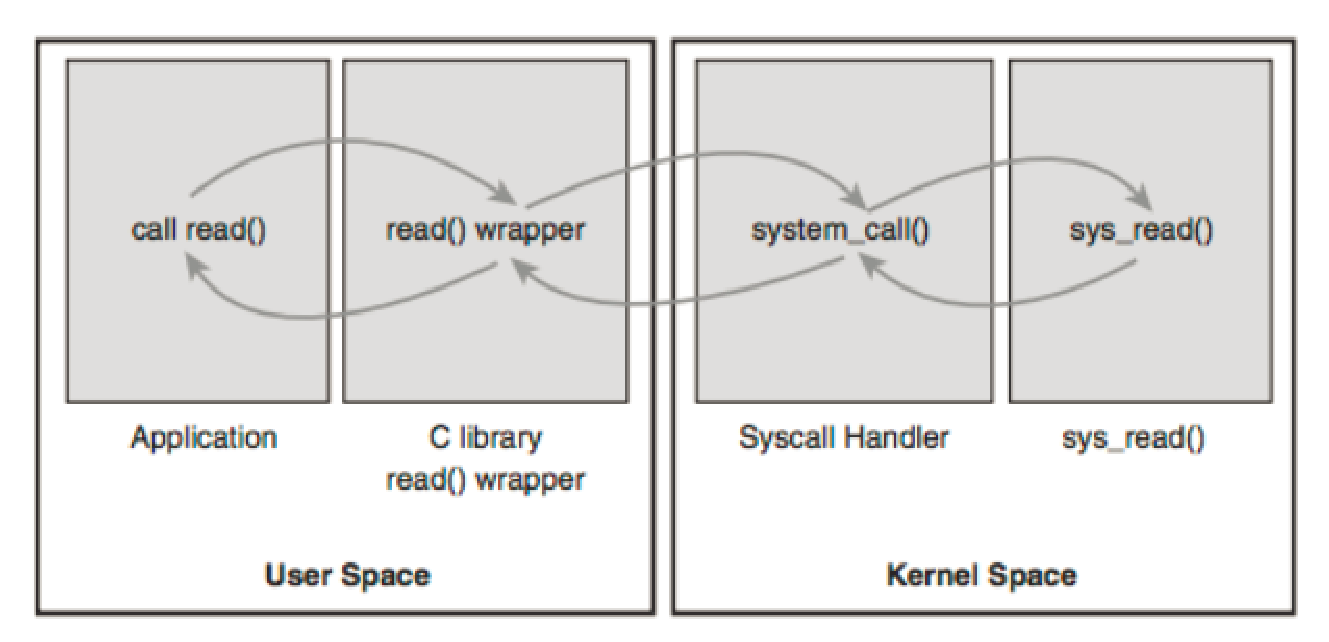
\includegraphics[height=3cm,
    angle=0]{./images/API-call-chain.eps}}
\caption{From a regular functional call to a system call}
\label{fig:API-call-chain}
\end{figure}


\subsection{-- glibc (libc)}
%\label{sec:glibc}

\verb!libc! (Sect.\ref{sec:libc}) is the early fork of glibc.
Later on, glibc is widely adopted (Sect.\ref{sec:glibc}).

So libc is just one of the libraries provided by glibc - and there are other
alternate implementations of libc other than glibc.

Note that not all standard C functions are in libc - most math functions are in
\verb!libm! (Sect.\ref{sec:libm}).
However, the glibc (GNU libc) project provides more than just libc - it also
provides the libm mentioned earlier, and other core libraries like
\verb!libpthread!.

\subsection{-- CRT (Microsoft)}

Sect.\ref{sec:CRT}

\subsection{musl}
\label{sec:musl}

musl is a 'libc', an implementation of the standard library functionality
described in the ISO C and POSIX standards, plus common extensions, intended for
use on Linux-based systems.

\url{http://www.musl-libc.org/faq.html}

\section{Standard C++ library implementation}
\label{sec:standard-C++-library}
\label{sec:C++-standard-library}

A standard C++ library provides system-level APIS implemented based on C++
language standard for a certain operating system.
Most C++ standard libraries are implemented over the OS's C library
(Sect.\ref{sec:standard-C-library}).


\begin{itemize}
  
  \item libstdc++ (implementation for GNU g++ compiler - Sect.\ref{sec:GCC}):
  on GNU/Linux.

Linux components have been developed around GNU libstd++ for ages. Some of them
do not build on anything else.


  \item libc++ (implementation for clang++ compiler - Sect.\ref{sec:clang}): on
  Mac O/S
  
\begin{verbatim}
clang++ -stdlib=libc++
\end{verbatim}

While libc++ is strong in new features, it has some problems with legacy code.
\end{itemize}


Example:
The libstdc++ std::string is a different data structure than the libc++
std::string. The former is a reference counted design, whereas the latter is
not. Although they are API compatible, they are not ABI compatible. That means
that if you construct a std::string with libstdc++, and then pass it to other
code that is linked against libc++, the receiving code would think it has a
libc++ std::string.
To you the programmer the libstdc++ std::string and the libc++ std::string look
like the same type. But to the linker, they look like completely different types
(the clue is the \verb!std::__1! namespace). And the linker's view is correct.
They are completely different types.
\begin{verbatim}
  // libstdc++
std::string, required to be resolved against std::basic_string implementation.

  // libc++
std::string, required to be resolved against the std::__1::basic_string implementation
\end{verbatim}
\url{http://stackoverflow.com/questions/12542971/using-libstdc-compiled-libraries-with-clang-stdlib-libc}

The pre-C++11 gcc std::list is not ABI compatible with the C++11 spec of
std::list. So, libc++ is no more ABI incompatible
with pre-C++11 libstdc++ than a C++11-conforming libstdc++ will be.


\subsection{-- libc++ (LLVM)}
\label{sec:libc++}

\verb!libc++! is the standard C++ library implemented on Mac O/S (since
Marvericks), and being used by clang/clang++ compiler, as well as GCC 4.7+.
\begin{itemize}
  \item On OS X before Mavericks: libstdc++ (Sect.\ref{sec:libstdc++}) was the
  default.
\end{itemize}
Compile the code using libc++ library with \verb!-stdlib=libc++! flag, and 
\verb!-std=c++11! flag.

\begin{verbatim}
g++ -std=c++11 -stdlib=libc++ input.cxx -o a.out
g++ -std=gnu++11 -stdlib=libc++ input.cxx -o a.out
clang++ -std=c++11 -stdlib=libc++ input.cxx -o a.out
clang++ -std=gnu++11 -stdlib=libc++ input.cxx -o a.out
\end{verbatim}

NOTE: libc++ is a new implementation of the C++ standard library, targeting C++11
(Sect.\ref{sec:C++11}). libc++ is not 100\% complete on GNU/Linux, and there's
no real advantage to using it when libstdc++ is more complete.
\url{http://libcxx.llvm.org/docs/}



\subsection{-- libstdc++ (GNU)}
%\subsection{libstdc++ : standard C++ library}
\label{sec:libstdc++}

\verb!libstdc++! is the standard C++ library implemented for GNU C++ Compiler
(Sect.\ref{sec:GCC}).
\begin{itemize}
  \item libstdc++ version 5: mainly needed for older pre-compiled packages
  
  \item libstdc++ version 6:
\end{itemize}
As libstdc++ is tightly integrated with g++ compiler development,
development of libstdc++ tending to be tied fairly closely to the matching
version of g++.

On Linux: In general, all commonly available linux distributions will use
libstdc++ by default.

\begin{verbatim}
clang++ -std=c++11 input.cxx -o a.out
clang++ -std=gnu++11 input.cxx -o a.out
\end{verbatim}

libstdc++ 4.2 is the last version using GPL2 license.

libstdc++ 4.3+ uses GPL3 license.

\subsection{-- libstdcxx (Apache)}
\label{sec:libstdcxx}

It lacks C++11 supports, as it is discontinued, i.e. STDCXX 4.2.1 in May'08.

\subsection{-- STLport}

It lacks C++11 supports, as it is discontinued, i.e.
STLport 5.2.1 was released in Oct'08.

\subsection{-- C++RT (Windows)}

Sect.\ref{sec:C++_RT}.

\section{Write a static library}

\subsection{In Linux}

In C, we do
\begin{verbatim}
cc -Wall -c ctest1.c ctest2.c 

// static library
ar -cvq libctest.a ctest1.o ctest2.o

\end{verbatim}
then
\begin{verbatim}
// linking to executable
cc -o executable-name prog.c libctest.a

cc -o executable-name prog.c -L/path/to/library-directory -lctest
\end{verbatim}

\subsection{Visual Studio}

Create a static library using Visual Studio for C/C++ (Sect.)



\section{Write an DLL}

\subsection{In Linux}

For shared library, we do
\begin{verbatim}
gcc -Wall -fPIC -c *.c
gcc -shared -Wl,-soname,libctest.so.1 -o libctest.so.1.0   *.o
mv libctest.so.1.0 /opt/lib

// create the default version using symbolic link
ln -sf /opt/lib/libctest.so.1.0 /opt/lib/libctest.so
ln -sf /opt/lib/libctest.so.1.0 /opt/lib/libctest.so.1
\end{verbatim}

We use 
\begin{enumerate}
  \item \verb!-fPIC! to produce position-independent code, 

  \item  \verb!-shared! to produce a shared object (*.so) which can be linked with
  other objects to form an executable.

\end{enumerate}

Then
\begin{verbatim}
gcc -Wall -I/path/to/include-files -L/path/to/libraries prog.c -lctest -o prog

gcc -Wall -L/opt/lib prog.c -lctest -o prog

\end{verbatim}


%\subsection{Export DLL's APIs}
\subsection{In Windows (C/C++)}
\label{sec:__declspec(dllexport)}

Writing a DLL in Windows is similar writing code for a static .LIB in Windows,
except we need to explicitly specify which APIs are accessible from outside the
library.


Not all APIs defined in the DLL can be accessed by the code that link to the
DLL. You have two options:
\begin{enumerate}
  \item use a Microsoft specific identifier  \verb!__declspec(dllexport)! declaration in the function definition 
\url{https://msdn.microsoft.com/en-us/library/dabb5z75(VS.80).aspx}

  
Example: C++ code  
\begin{verbatim}
// header file
#ifndef ADD_H
#define ADD_H
int __declspec(dllexport) add(int a, int b);
#endif  // ADD_H
\end{verbatim}

and in the program that use the library 
\begin{verbatim}
#include "add.h"
int add(int a, int b) {
    return a + b;
}
\end{verbatim}
  
  \item
\end{enumerate}

Example: \verb!extern ``C''! is important with C code. 
\begin{verbatim}
#include <stdio.h>

extern "C"
{
  __declspec(dllexport) void DisplayHelloFromDLL()
  {
    printf ("Hello from DLL !\n");
  }
}
\end{verbatim}
\verb!__declspec(dllexport)! is a required prefix for all functions that we
want to make DLL functions available from an external application.


Example: 
\begin{verbatim}
#include <iostream>
#include "cuda.h"
#include "cuda_runtime.h"
#include "device_launch_parameters.h"

extern "C" __declspec(dllexport) int sumTEst(int a, int b)
{
    int c = 0;
    test<<<1,1>>>(a, b, &c);
    return c;
}
\end{verbatim}  

Now we can build and get a DLL.

In Visual Studio, we can create a DLL project
\begin{verbatim}
File/New Project (Ctrl-Shift-N)
   Visual C++ project
      Template: Win32 project
 
Name of Project: <DLL name>

Application Settings (Application Type): choose DLL
Check Empty Project 
\end{verbatim}
\url{http://www.codeproject.com/Articles/9826/How-to-create-a-DLL-library-in-C-and-then-use-it-w}

\begin{mdframed}

A shared library can be in 1 or 5 states when it comes to debug/release DLLs.
To investigate a DLL, in Windows, we can use \verb!ilDasm.exe! utility.

\begin{enumerate}
  \item A non-debugable DLL
  \item An optimized debug DLL
  \item An optimized release DLL
  \item A non-optimized debug DLL
  \item A non-optimized release DLL
\end{enumerate}

\end{mdframed}


Initially, one \verb!.cpp! file whose name the same name as the project; and
\verb!stdafx.cpp! file which is necessary (yet you don't need to edit it - Sect.\ref{sec:stdafx.h})
% To create a DLL project: 
% \begin{itemize}
%   \item File / New Project (Ctrl-Shift-N)
%   \item Visual C++ Templates: select win32 project
%   \item Application Settings: select DLL
% \end{itemize}


Add a new C++ source file, and enter functions. These functions can be exposed
as APIs or just for internal use. Those exposed as APIs can be called by other
codes that reference to this DLL.
Sect.\ref{sec:__declspec(dllexport)} describes how to expose an API.

Now, to build this code into DLL, we need to use \verb!/LD! option in Visual Studio (Sect.\ref{sec:building_DLL_/LD}).

\subsection{Entry point of DLL}

Every application, including library, needs entry point. It is the address that
is used to load in to CPU PC register. It's similar to an entrance in a
building. You can go everywhere on every of that 100 storeys and thousands of
offices but there is only one entrance. The entry point of a DLL is
\verb!__DllMainCRTStartup! for 32-bit DLL and \verb!_DllMainCRTStartup! for
64-bit DLL. The function calls \verb!DllMain()!, and if there is no
\verb!DllMain()!, the DLL will not be loaded.



A DLL can optionally specify an entry-point function. If present, the system
calls the entry-point function whenever a process or thread loads or unloads the
DLL. It can be used to perform simple initialization and cleanup tasks. For
example, it can set up thread local storage when a new thread is created, and
clean it up when the thread is terminated.

The \verb!DllMain! function is an optional entry point into a dynamic-link
library (DLL). However, as \verb!DllMain! is a placeholder for the
library-defined function name, you can define a different name as the entry
point using the \verb!/ENTRY:linker! option and name your entry-point function
something other than DllMain, the C run-time library will not get initialized
properly. Nevertheless, if you decide to write your own entry-point funciton, it
has to duplicate everything that \verb!_DllMainCRTStartup! does
(NOTE: 
.
When building DLLs in Visual C++, \verb!_DllMainCRTStartup! is linked in automatically
and you do not need to specify an entry-point function using the /ENTRY: linker
option.


Examples of entry point function:
\begin{verbatim}
int main() for consoles

WinMain() for Win32-GUI

DLLMain() for DLL's
\end{verbatim}
Sect.\ref{sec:without_main()} describes how use a different name for the entry-point in a console application.

IMPORTANT:  Don't call CreateProcess from DllMain, as it can create dead lock.
he standard way to get things done from DllMain is to create a thread to do the
work.
Calling functions that require DLLs other than Kernel32.dll may result in
problems that are difficult to diagnose.
For example, calling User, Shell, and COM functions can cause access violation
errors, because some functions load other system components.
 Conversely, calling functions such as these during termination can cause access
 violation errors because the corresponding component may already have been
 unloaded or uninitialized.

\section{Using a LIB in your project}

By default, all the symbols in a static library are visible to the linker and available for the linked program. 

Of course to compile your program you need the matching header (normally .h)
files of the static library. A static library has nothing to do with .def or
.exp files.

\section{Using a DLL in your project}

In order to compile an executable file (Sect.\ref{sec:executable_file}) using a
DLL, you need to tell the linker how the DLL can be used when linking.
The header file can only give some information, e.g. the function signature. But
the compiler still need to know the name of the DLL, and what symbols are
available in the DLL. This information can be stored in either
\begin{enumerate}
  \item an import library (Sect.\ref{sec:import_library})
  
The import library (.LIB) is automatically created when you compile a DLL file.
   
  \item a .exp file (export file): 
  
\end{enumerate}

We need both the header file and the binary files. 
\begin{itemize}
  \item Tell the compiler where to  look for your header files
  
  \item Tell the linker where to look for the library files (static or import
  libraries) 
  
There is no need to configure if dynamic library is used.
  
  \item \verb!#include! the header files in your program 
  
  \item (if dynamic libraries or import library is used) then make sure the
  location of the dynamic libraries can be found by the program at runtime.

The .dll file must be available when the executables run at run-time. 

\end{itemize}

In Visual Studio, read Sect.\ref{sec:VS_Configuration_Properties}

\subsection{Troubleshoot DLL version mismatch}

Many third-party uses C/C++ Runtime Library (Sect.\ref{sec:CRT},
Sect.\ref{sec:C++_RT}). However, this can cause a conflict issue when you use
one third-party DLL compiled using Visual Studio 2005, while the other
third-party DLL was compiled using Visual Studio 2008. Two versions of VS use
two different version of the CRT (Sect.\ref{sec:CRT}).

To know which CRT version was used to compile a DLL, we use \verb!DUMPBIN! tool (Sect.\ref{sec:dumpbin_command}). 
\begin{verbatim}
dumpbin /imports <dllname.dll>
\end{verbatim}
and search for MSVCRT**.dll, with \verb!**! will be the version number (70, 71, 80, 90). 


Suppose you are the third-party who develop the DLL. It is best to fix the same 
version of Runtime Library, regardless of which version of Visual Studio you use. 
This can be done by
\begin{enumerate}
  \item disable using default RunTime libraries
\begin{verbatim}
Project Properties->Linker->Input->Ignore All Default Libraries->Yes
\end{verbatim}

  \item create a custom library and link that to the project
\url{https://msdn.microsoft.com/en-US/library/k9a8ehy3(v=VS.80).aspx}
  
Microsoft VS allows you to compile your own version of CRT.
\begin{itemize}
  \item Run the Visual Studio Command Line tool as Administrator
  
  \item type
\begin{verbatim}
set vctools=C:\Program files\Microsoft Visual Studio x.x\VC
\end{verbatim}
with \verb!x.x! is the version of the Visual Studio.

  \item type
\begin{verbatim}
crt\src\bldnt.cmd
\end{verbatim}

This will run for a minute or so, compiling all the necessary libraries for your system, which returns
\begin{verbatim}
libcmt.lib
libcpmt.lib
_sample_.dll
_sample_.lib
\end{verbatim}
NOTE: \verb!_sample_.*! are the actually copies of msvcrXX.dll (where XX is your VS version). 
They are renamed so that they do not conflict with the actual MS libraries.


\end{itemize}

To compile a custom version of CRT that you can pack with your library.

\begin{verbatim}
'Additional Dependencies=.\_sample_lib'
\end{verbatim}
  
The other alternative is just to ignore the default CRT libraries by going to
'Ignore Specific Library=msvcr9.0.lib' and place
\begin{verbatim}
'Additional Dependencies '_sample_.lib' 
\end{verbatim}
so that your library relies on your compiled library and not the
system defaults.

This allows for greater flexibility when sharing your libraries with customers,
as your dependencies get shipped along with your libraries.

\url{http://www.codeproject.com/Articles/85391/Microsoft-Visual-C-Static-and-Dynamic-Libraries}  
\end{enumerate}




\subsection{DLL hell}
\label{sec:DLL_hell}

DLLs were introduced with the first releases of Windows.
DLLs were not only introduced for the core OS, but made available for programs
as well. Microsoft frameworks such as MFC, .NET, ATL, GdiPlus, etc. as well as
for the C (CRT) and C++ runtime libraries made use of DLLs.

Everything would have been okay if the implementation of DLLs would have been
clean and non-ambiguous. Unfortunately that wasn't the case, as Microsoft and
others began releasing different versions of the same (system and non-system)
DLLs that had no proper versioning.

Most applications installed their DLLs in the system directory (and many still
do) in hope to share them with other programs but there was no way to keep two
different versions of a DLL in the system folder as the file name usually
remained unchanged. Then, installing an application could possibly break other
applications (because they were build for a different "version" of the DLL) and
the new installation delete the old DLL file to replace with a new one.
And even worse, uninstalling an application could remove some DLLs that other
 applications depended on. This is called {\bf DLL
hell}.
\footnote{\url{http://www.drdobbs.com/windows/no-end-to-dll-hell/227300037}}

.NET Frameowork tried to resolve this problem by introducing the concept
{\bf side-by-side execution}
\footnote{\url{http://msdn.microsoft.com/en-us/library/8477k21c(v=vs.110).aspx}}
using the so-called Global Assembly Cache.
However, it cannot completely avoid the problem.
The best way to defeat all DLL conflicts is don't use any DLLs at all, but use
static libraries instead. However, this will make the final executable file too
big. Another, that allows using DLL is to include all DLL in a private folder in
the application bin-directory and use private assemblies as far as possible if
assemblies cannot be avoided.

\url{http://stackoverflow.com/questions/1379287/i-keep-hearing-about-dll-hell-what-is-this}

\section{Using nm utility}
\label{sec:using-nm-utility}


{\bf nm} utility allows us to investigate the symbolic names of the
functions defined in the library.
\begin{lstlisting}
nm my_library.a

nm my_library.so
\end{lstlisting}

References:
\begin{itemize}
\item \burl{http://wordaligned.org/articles/hunting-down-globals-with-nm}
\item  \burl{http://www.calvin-studio.fr/docs/Cplusplus/susv3/utilities/nm.html}
\end{itemize}


\section{Link error with vector type and /MD (multi-threaded)}

When you try to build your library with multi-threaded option enabled (/MD) and
using vector type, you can get  linker error 
\begin{verbatim}
 vector<int>& Parameters
 int parameter2 = Parameters.at(1);  //generates a linker error:

CUDAFluxEngine.cu.obj : error LNK2019: unresolved external symbol
__imp__CrtDbgReportW referenced in function "public: char & __cdecl
std::vector<char,class std::allocator<char> >::operator[](unsigned __int64)"
(??A?$vector@DV?$allocator@D@std@@@std@@QEAAAEAD_K@Z)  
\end{verbatim}

The vector class is going to want to tell you that the at() method failed in
debug mode.  Thus the reference to CrtDbgReportW(), the runtime function that
displays diagnostics while debugging.  When you link with /MD, you link with the
release version of the run-time library; the one that doesn't tell you anything
and is missing the CrtDbgReportW() export.  Thus the linker error.    

So, make sure in Debug mode, you choose \verb!/MDd!; while in Release mode, you
choose \verb!/MD!. I'm guessing that using the Multi-Threaded DLL
debug option uses the debug runtime library "msvcrtd.dll", which replaces the
normal runtime library \verb!msvcrtd.dll!.

\url{https://social.msdn.microsoft.com/Forums/en-US/5fcad5be-f597-40fa-8912-9bb3d8ade853/linker-error-with-vector-use-multithreaded-dll-config}

% You can fix this by removing the \verb!_DEBUG! define from the preprocessor
% definitions.  If you don't want to lose that valuable tool, tell us what goes
% wrong when you link with /MDd.  



\section{COM (Component Object Model)}
\label{sec:COM}

Approaches like ATL promotes the reuse of source codes.
COM, on the other hands, promote the reuse of binary codes.
COM is, simply put, a method for sharing binary code across different
applications and languages.

Dynamically linked libraries (Sect.\ref{sec:DLL}) like kernel32.dll, user32.dll
are written in C, and thus can be used only by C or a language that understand
the C calling convention.

{\bf COM } defines a binary standard, and specifies exactly how COM objects are
organized in memory. This allows a code written in one language to be able to
read a binary objects or calling a function written in another language easily.

The structure of COM objects in memory just happens to use the same structure
that is used by C++ virtual functions, so that's why a lot of COM code uses C++.
But remember, the language that the module is written in is irrelevant, because
the resulting binary is usable by all languages.


Incidentally, COM is not Win32-specific. It could, in theory, be ported to Unix
or any other OS. However, I have never seem COM mentioned outside of the Windows
world.

\url{http://www.codeproject.com/Articles/633/Introduction-to-COM-What-It-Is-and-How-to-Use-It}


Component Object Model (COM) is a method to facilitate communication between
different applications and languages. It is a binary standard to enable
software components to interop in a networked environment regardless of the
computing languages in which they were developed. To handle and report errors,
Transaction Integrator (TI) is developed as a standard way. 

Component Services (COM+) consist (1) the latest version of COM, i.e.
distributed COM (DCOM) and (2) Microsoft Distributed Transaction Coordinator
(DTC), plus additional functionality. 

COM and COM+ are the key technologies that provide the infrastructure that
enables clients and objects to work together. Other key COM concepts include
methods, interfaces, classes, references, and components, which build on the
foundation of clients and objects. COM components are unmanaged C++ code
components designed to make software reusable at binary level.

To create a COM, COM+, C++ is the most "natural" language in COM, but COM
components can be created in MANY languages (C\#, VB.NET). To create .NET
component, we need to use a .NET language project (C\#, VB.NET). 
\url{http://stackoverflow.com/questions/688456/what-is-the-difference-between-net-components-and-com-components}

\subsection{Access COM APIs from C++}

For calling COM components based on Interface Definition Language (IDL), the
suggestion is to use C++ interop. The C++ layer can be very thin and the rest of
the managed code can be written in any managed language 


\section{DCOM (Distributed COM)}
\label{sec:DCOM}


DCOM is a method that allow invoking a COM object regardless of its location (local or remote) to the calling process.



\section{Dynamic Load Library}
\label{sec:dynamic-load-library}

Dynamic Load Library refers to the technique that allow a program to
invoke the functions defined in a static or shared library while this
library can be built from the source code written in the same or
different language with the current code.

\subsection{In C}
\label{sec:dynamic-load-library-in-c}
\label{sec:dlopen}

If the library compiled from C language, the common way to load APIs defined in
a library is to (1) link to \verb!-ldl! (dl = dynamic loading, i.e. libdl
library), and (2) use the following APIs.
\begin{verbatim}
void *dlopen(const char
void *dlsym(void *handle, char *symbol);
const char *dlerror();
int dlclose(void *handle);
\end{verbatim}

These APIs allow loading a C functions, as defined in another shared library, at runtime.
See the example below.

\begin{lstlisting}
// bar.c 
// reference to an external function 'foo'
extern void foo(void);

void bar(void)
{
  foo();
}

// main.c
#include <dlfcn.h>
#include <stdio.h>
#include <stdlib.h>


void foo(void)
{
  puts("Hello World!");
}


int main(void)
{
   void* dlh = dlopen("./libbar.so", RTLD_NOW);
   
   if (!dlh) {
      fprintf(stderr, "%s\n", dlerror());
      
      exit(EXIT_FAILURE);
   }
   
   void (*bar)(void) = dlsym(dlh, "bar");  // 'bar' variable is now a pointer 
          // pointing to the "bar" function defined in the 
          // loaded library
          
   bar();   // use 'bar' variable as a function now
 
}
\end{lstlisting}

Basically, we use \verb!dlopen! to load the library and use
\verb!dlsym! to read the required function by passing the function
name in string. We use \verb!dlerror! to detect error and
\verb!dlclose! to unload the library.


The Makefile for the above code
\begin{verbatim}
.PHONY: all clean test

LDFEXTRAFLSGS ?= 

all: prog

bar.o: bar.c
   gcc -c -Wall -fpic -o $@ $<
   
   // make a shared library
   // which use a function 'foo' that is defined by the program
   // then we need to link such program using -rdynamic 
   //   or -Wl,--export-dynamic
libbar.so: bar.o
  gcc -shared -o $@ $<
  
  
prog: main.o | libbar.so
   gcc $(LDEXTRAFLAGS) -o $@ $< -L. -lbar -ldl
   
   // this is where the function 'foo' is defined
main.o: main.c
   gcc -c -Wall -o $@ $<
\end{verbatim}

\subsection{symbol in a shared library}
\label{sec:symbol-shared-library}


\textcolor{red}{IMPORTANT: } When a function is compiled in binary form, it is
represented by a {\it symbol}, i.e. a special string that uniquely identify the
function in the whole program/module/library. In C, the symbol is the same as
the function name. In C, there is no concept of namespace, classes, so it's
impossible for two functions to have the same name.

In C++, the situation is a little bit more complicated as ``class''
are allowed in C++ and ``name mangling'' issue. We'll discuss in the
next section (Sect.\ref{sec:dynamic-load-library-in-c++}). 


Exported symbols are resolved by the dynamic - runtime - linker, through a
process of {\bf dynamic bindings} (Sect.\ref{sec:linker}).

Excutable programs don't usually need to export symbols, and they usually don't
export symbols at all. However, there are rare cases (as given below) where
executables are required to export symbols, e.g. the symbol is used by the
shared library that it loads. This is known as a 'callback' from the library to the program,
or for C++ programs for RTTI to properly work
\begin{verbatim}
program A has a symbol 'foo'
program A load the shared library 'lib_b' 
    shared library 'lib_b' has a function 'bar' which call an external function 'foo'
    
    // now at runtime, program A call 'lib_b   bar' funnction, which use the function 'foo' as implemented in program A
\end{verbatim}
To expose or export symbols, the program needs to be built using \verb!-Wl,--export-dynamic! 
or \verb!--rdynamic! option.

If not, i.e. does not export symbols, the symbols are hidden and thus resolved directly at buildtime


References:
\begin{itemize}
\item \burl{http://www.linuxjournal.com/article/3687}
\end{itemize}

\subsection{In C++}
\label{sec:dynamic-load-library-in-c++}

In C++, there are many new features that violate the above property of C
language (Sect.\ref{sec:dynamic-load-library-in-c}), e.g. function overloading
is a feature that allows two functions can have the same name, yet with
different function arguments. 

To deal with that, C++ compilers use the technique called {\it name mangling} to
generate the unique string based on the function name and other information
(e.g. class name, argument name...). There is no standard for this, so different
compilers can use different technique, and thus it's impossible to know the
symbols for the function in binary form.

\subsubsection{Static functions}
\label{sec:static-functions}

As C++ is a superset of C, it means that we still can define \verb!static!
function in C++. These static functions are not class member functions.  C++
thus provide a special keyword \verb!extern ``C''! that tells the compiler to
use the function name as the symbol. By doing this, user can easily load the
function written in C/C++ from other languages, e.g. Fortran.
\verb!extern ``C''! is a very powerful feature as the function can use full C++
features, it's only the function name are kept during compilation.

We can do
\begin{lstlisting}
extern "C" int foo;
extern "C" void bar();

extern "C" int foo;

\end{lstlisting}
or
\begin{lstlisting}
extern "C" {
     extern int foo;
     extern void bar();
    int foo;
 }
\end{lstlisting}
or we can use the macro \verb!__cplusplus! (Sect.\ref{sec:__cplusplus}) so that
the file can be used for both C and C++. 
\begin{lstlisting}
#ifndef _STDIO_H
#define _STDIO_H
#ifdef __cplusplus
  extern "C" {
#endif /* __cplusplus */
.
. /* Functions and data types defined... */
.
#ifdef __cplusplus
  }
#endif /* __cplusplus */
#endif
\end{lstlisting}

\subsubsection{Class member function}
\label{sec:classs-function}

In C++, we cannot use \verb!extern! on class member functions.  For
class functions, we need to know the instance of the class, beside the
pointer to the function.  We cannot create a class instance from C and
Fortran. So, there is no direct mechanism to load classes at runtime
from C or Fortran.  The only way to work with C++ class is to create a
function in C++ that do the proper construction and destruction, and
then return the pointer to the instance of the object.  We define a
base class called entity.
\begin{lstlisting}
class entity {
private:
   float xyz[3];  // position of the object
public:
   activate(float)=0; // tell the object to move
   render()=0;  // tell the object to draw itself
};
\end{lstlisting}
or we use an interface class that contains only virtual members in the
executable. Generally the interface class is abstract (a class is
abstract if it has pure virtual functions).
\begin{lstlisting}
class image_handler{
public:
   virtual Image loadImage(char *)=0;
   virtual int saveImage(char *, Image &)=0;
};
\end{lstlisting}
and a derived, implementation class in the module.

Next, while still in the module, we define two additional helper
functions, known as class factory functions. One of these functions
creates an instance of the class and returns a pointer to it. The
other function takes a pointer to a class created by the factory and
destroys it. These two functions are qualified as extern "C".
\begin{lstlisting}
map <string, handler, less<string>> handler_map;
char *filename = "flower.tiff";
char ext[MAX_EXT_LEN];

howEverYouWantToParseTheExtensions(filename, ext);
// after parsing "flower.tiff" ext = "tiff"<\n>
Image img1 = handler_map[ext]->loadImage(filename);
// process data here
handler_map[ext]->saveImage(filename, img1);
\end{lstlisting}



\begin{itemize}
\item \burl{http://www.faqs.org/docs/Linux-mini/C++-dlopen.html}
\item \burl{http://www.parashift.com/c++-faq-lite/mixing-c-and-cpp.html}
\end{itemize}

\subsection{Fortran}
\label{sec:fortran-2}

For a library written in Fortran and want to be invoked from 

% \section{Static/Shared Dynamic - loadable libraries Linux}
% \label{sec:stat-dynam-load}
% 
% The technique {\bf shared components} or {\bf archive libraries}
% requires
% \begin{enumerate}
% \item compile the source files into object files, 
% \item group them into a single .a file (static) or .so (dynamic). This
%   is known as the static library or dynamic library, respectively.
%   The C standard libraries and C++ STL are examples of shared
%   components which can be linked with your code.
% \end{enumerate}


\chapter{C/C++ in Linux: glibc, libstdc++/libc++}
\label{chap:CCpp_Linux}

Chap.\ref{chap:CCpp_Windows} will discuss APIs' implementation of C/C++ standard
specification for Windows O/S.
In this chapter, we will discuss API's implementaiton of C/C++ standard
specification for Linux-based O/S and how to write portable code across platform
(Sect.\ref{sec:CCpp_portable-code}).

The Linux kernel is written in C language and the access to the underlying CPU
platform is exposed to users through a set of C-language-based APIs implemented
in a library, which can be either
\begin{enumerate}
  \item POSIX C library (Sect.\ref{sec:POSIX-C-library})
  
  \item C standard library (Sect.\ref{sec:C-standard-library})
\end{enumerate}

%{\bf glibc}.

\section{How the Linux O/S runs a program (ld-linux.so.2)}
\label{sec:how-linux-run-a-program}

The GNU dynamic loader (e.g. \verb!/lib/ld-linux.so.2!) is one of the main
components of the user space in a Linux-based system.

The main task of the dynamic loader is to handle the interaction between the
program and the system's shared libraries by relocating unresolved symbols.


Your executable program is compiled with a given version of GCC
(Sect.\ref{sec:GCC}) which indeed utilizes the APIs as provided by the standard
C or C++ library, i.e. uses a given version of \verb!libstdc.so! or
\verb!libstdc++.so! (Sect.\ref{sec:libstdc++}), this \verb!libstdc++.so! was
compiled and is depending upon a particular version of another library, e.g.
\verb!libgcc_s.o! for example. So, always there is a chain of version
dependency.
  
  
\textcolor{red}{Now, what is actually your executable program?}
\begin{itemize}
  
  \item Under Linux, and on most modern Unix(es), an executable program is just
  the same kind of file of a shared object or shared library
  
  And exactly as shared library, they can also export symbols (Sect.\ref{sec:symbol-shared-library}).
  
  \item 
\end{itemize}

% \begin{itemize}
%   \item 
%   \item the extension for a given compiler is written in C++, which may takes
%   advantage of newer C++ features so it is compiled by a newer version GCC or in
%   other case compiled by an older version of GCC, which in either cases depends
%   on a different version B of \verb!libstdc++.so!
% \end{itemize}


Issues when you try to run your program
\begin{enumerate}
  \item no available dynamically linked library, e.g. \verb!libstdc++.so!, for the program to use
  
\begin{verbatim}
$> ./myapp   

./myapp: error while loading shared libraries: libstdc++.so.6: cannot open shared object file: No such file or directory
\end{verbatim}
SOLUTION: Copy \verb!libstdc++.so.6! 


  \item not the same version of the libstdc++ used to compile the program
\begin{verbatim}
$> ./myapp  

./myapp: /usr/lib64/libstdc++.so.6: version `GLIBCXX_3.4.15` not found ( required by myapp )
\end{verbatim}
EXPLAIN:  As gcc evolves, so do the contents of libstdc++ library, i.e. 

SOLUTION: use the right version, e.g. \verb!libstdc++-4.5.1.so!
\begin{verbatim}
libstdc++.so.6       ---> libstdc++-4.5.1.so
\end{verbatim}

We may want to specify the path of the shared library via \verb!LD_LIBRARY_PATH!
\begin{verbatim}
$>LD_LIBRARY_PATH=libs/ ./myapp   

Hello!
\end{verbatim}

We can check the library dependencies, i.e. one library file uses which other
library files
\begin{verbatim}
$>LD_LIBRARY_PATH=libs/ ldd ./myapp  

linux-vdso.so.1 => (0x00007fffbe9f2000) 
libstdc++.so.6 => libs/libstdc++.so.6 (0x00007fcb13b85000) 
libc.so.6 => /lib/x86_64-linux-gnu/libc.so.6 (0x00007fcb1379b000) 
libm.so.6 => /lib/x86_64-linux-gnu/libm.so.6 (0x00007fcb13496000) 
/lib64/ld-linux-x86-64.so.2 (0x00007fcb13e8b000) 
libgcc_s.so.1 => libs/libgcc_s.so.1 (0x00007fcb13280000)
\end{verbatim}

We can check the ELF
\begin{verbatim}
$> readelf -d myapp
[...]
0x00000001 (NEEDED)                     Shared library: [libtest.so]
0x00000001 (NEEDED)                     Shared library: [libc.so.6]
\end{verbatim}

  \item to eliminate the use of \verb!LD_LIBRARY_PATH! every time you run the program:
  (1) put that setting in the \verb!~/.bashrc! file, (2) compile your program and specify the user-defined path to look for the 
  shared library via \verb!rpath! option
  
\begin{verbatim} 
 // only look for shared library in the default system search path 
 //   (defined in ld.so and ldconfig)
g++ -o myapp myapp.cpp

 // use rpath option
 // with the special token $ORIGIN which causes ld.so to locate
 //    the shared libraries relative to the location of the binary 'myapp'
g++ -Wl,-rpath=\$ORIGIN//lib myapp.cpp -o myapp

 // more flexible
g++ -Wl,-rpath=\$ORIGIN//lib --enable-new-dtags myapp.cpp -o myapp
\end{verbatim}
Sect.\ref{sec:linker} explains how to hard-code a path to a shared library.

We can check the \verb!.dynamic ELF! section
\begin{verbatim}
$> readelf -d main
[...]
0x00000001 (NEEDED)                     Shared library: [libtest.so]
0x00000001 (NEEDED)                     Shared library: [libc.so.6]
0x0000000f (RPATH)                      Library rpath: [$ORIGIN]
\end{verbatim}
The \$ORIGIN variable within the \verb!DT_RPATH! value refers to the current execution directory of the main program.

The general drawback using \verb!DT_RPATH! is that you cannot overwrite this
embedded path setting with \verb!LD_LIBRARY_PATH!. This limits the flexibity of
using shared libraries. There are two options: (1) remove the shared library
from the given path, (2) use \verb!-enable-new-dtags! compiling option which set
the value in \verb!DT_RUNPATH!.
In the later option, the dynamic loader searches the \verb!LD_LIBRARY_PATH!
before the embedded path in the executable.
\url{http://blog.lxgcc.net/?tag=dt_runpath}

  \item we have the right version of \verb!libstdc++.so.6!, but this library depends on another 
  library whose version is not correct
\begin{verbatim}
$> ./myapp

myapp: /lib/x86_64-linux-gnu/libc.so.6: version `GLIBC_2.14' not found (required by libs/libstdc++.so.6)
\end{verbatim}  
EXPLAIN: \verb!libstdc++.so.6! requires version 2.14 of \verb!libc.so.6!, but the system cannot find this version.

SOLUTION: we may do the similar approach, i.e. copy the right version of
\verb!libc.so.6!.


   \item But chances are you will broke your system if you change the
   \verb!libc.so.6!
versions as other programs, e.g. the Linux kernel, may depends on the existing
version of libc.so.6.

\begin{verbatim}
$> ./myapp  

FATAL: kernel too old  
Segmentation fault
\end{verbatim}
SOLUTION: No solution as replacing the Linux kernel is not a good option.
  
\end{enumerate}
\url{http://www.crankuptheamps.com/blog/posts/2014/03/04/Break-The-Chains-of-Version-Dependency/}

\subsection{libc.so.6}

32-bit version
\begin{verbatim}
/lib/i386-linux-gnu/libc.so.6
\end{verbatim}

64-bit version
\begin{verbatim}
/lib/x86_64-linux-gnu/libc.so.6
\end{verbatim}

This 
\begin{verbatim}
/usr/lib/x86_64-linux-gnu/libc.so
\end{verbatim}
 is not a library, but a linker script file, which refers to the above symlinks.
 
 
 First, regardless of libc version installed, the linker will always search for
 libc.so, because the compiler driver will always pass to the linker the -lc
 options. The name libc stays the same and denotes to most recent version of the
 library. The symlinks libc.so.6 are named after the soname of the library,
 which, more or less corresponds to the ABI version of the library. The
 executables, linked against libc.so in fact contain runtime dependencies on
 libc.so.6.

The file is created when you compile glibc 
\begin{verbatim}
#>cat /usr/lib64/libc.so
 
/* GNU ld script
   Use the shared library, but some functions are only in
   the static library, so try that secondarily.  */
OUTPUT_FORMAT(elf64-x86-64)
GROUP ( /lib64/libc.so.6 /usr/lib64/libc_nonshared.a  AS_NEEDED ( /lib64/ld-linux-x86-64.so.2 ) )
\end{verbatim}



\section{IMPORTANT: Understanding GNU C library (glibc) and its variants
(Linux libc, eglibc)}
\label{sec:POSIX-C-library}
\label{sec:library-implement-standard-C-language}

\verb!libc! refers to a specific implementation of the standard library
functionality described in ISO C and POSIX standards, optionally with common
extensions, intended for use on a Linux-based systems.

Whereas the kernel (Linux) governs access to hardware, memory, filesystems, and
the privileges for accessing these resources, the C library is responsible for
providing the actual C function interfaces userspace applications see, and for
constructing higher-level buffered stdio, memory allocation management, thread
creation and synchronization operations, and so on using the lower-level
interfaces the kernel provides, as well as for implementing pure library
routines of the C language like strstr, snprintf, strtol, exp, sqrt, etc.

A libc-type library is the core library that sits between user space and the
kernel. The first implementation of such library was named {\bf glibc}
(Sect.\ref{sec:glibc}) \verb!glibc! was first written mainly by Roland McGrath
from 1980s.

Then, a fork of glibc version, used in early Linux kernel, is \verb!libc!
(Linux libc) library.

\subsection{glibc (version 1, 2)}
\label{sec:glibc}
\label{sec:GLIBC}

{\bf glibc} is the first implementation of the standard specification for C
language (Sect.\ref{sec:library-implement-standard-C-language}).
Nowadays, Glibc is used in majority of distribution: Fedora-like, RHEL,
Debian-like, SuSE, Gentoo, Archlinux.

By 1988, glibc was supposed to have all features based on the standardization of
ANSI C language (Sect.\ref{sec:ANSI-C}). By 1992, features for ANSI C-1989 and
POSIX.1-1990 were also added. So, glibc is also known as POSIX C library.
glibc is known as GNU C library as it was first used by the GNU operating
systems and is managed by FSF (Free Software Foundation).

NOTE: {\bf glibc} is just one implementation of the C language specification
(Sect.\ref{sec:libc}). 

Nowadays, glibc version 2.x is not a single \verb!*.so! file - there are many.
It includes \verb!libc! (libc.so.6), and other essential libraries (\verb!libm!
for math, \verb!libpthread! for p-thread). Because of that, glibc is considered
as the C standard library (Sect.\ref{sec:C-standard-library}) and is being used
for Linux-like O/S or GNU/FreeBSD O/S. This library is also used by the Linux
kernel so is considered as a critical component of the Linux O/S.

Since 1995, Ulrich Drepper made his first contribution to the glibc project and
later become the main contributor. 

Since 2001, the development of glibc has been overseen by a committee, with
Drepper as the lead contributor.

Since 2012, the steering committee voted to disband itself and remove Drepper in
favor of a community-driven development process due to  the long standing
controversies around Drepper's leading style and external contribution
acceptance.

SUMMARY: glibc implements (more details see
Sect.\ref{sec:glibc-2.0})
\begin{enumerate}
  \item C library described in ANSI,c99,c11 standards. It includes macros,
  symbols, function implementations etc.(printf(),malloc() etc)
  
  \item POSIX C standard library. The "userland" glue of system calls.
  (open(),read() etc. 
  
  Actually glibc does not "implement" system calls. kernel does it. But glibc
  provides the user land interface to the services provided by kernel so that
  user application can use a system call just like a ordinary function.
  
  \item  some nonstandard but usefull stuffs.
\end{enumerate}

To tell the compiler to use a particular version of Standard C, we use \verb!-std=!
\begin{verbatim}
-std=c11
-std=gnu99
-std=c99
\end{verbatim}


\subsection{-- glibc 2.x (libc6)}
\label{sec:glibc-2.0}
\label{sec:glibc-2.x}

In Jan 1997, {\bf glibc 2.0} (or known as libc6 in Linux kernel -
Sect.\ref{sec:libc}) was released with (1) better internationlization, (2)
multilingual function, (3) IPv6 capability, (4) 64-bit data access, (5)
multithreaded support, (6) code more portable, (7) future version compatibility,
(8) more complete POSIX standards compliance than Linux libc
(Sect.\ref{sec:libc}).

Different versions of glibc 2.x
\begin{enumerate}

  \item glibc 2.3.4 (Dec. 2004): the standard for operating systems (O/S)
  following LSB-3.0 standard (Sect.\ref{sec:LSB_C-lang})
  
  \item glibc 2.4 (Mar 2006): with partial inotify support
  
  It is the standard for operating systems (O/S)
  following LSB-4.0 standard (Sect.\ref{sec:LSB_3.1}).
   

  \item glibc 2.5: full inotify support
  
\begin{verbatim}
* New Linux interfaces: splice, tee, sync_file_range, vmsplice (glibc 2.5)
* RFC 3542: Advanced socket interface for IPv6 (glibc 2.5)
* Support for the ELF .gnu.hash section (glibc 2.5)
* Real-time priority inheritance mutexes and priority protected mutexes
	(glibc 2.5)
\end{verbatim}
  
  \item glibc 2.6

\begin{verbatim}
* New Linux interfaces: epoll_pwait, sched_getcpu (glibc 2.6)
* New generic interfaces: strerror_l (glibc 2.6) 
\end{verbatim}

  \item glibc 2.7 (Oct 2007): used by Ubuntu 8.04 (Debian 5)

\begin{verbatim}
* New Linux interfaces: mkostemp, mkostemp64 (glibc 2.7)
* New Linux interfaces: signalfd, eventfd, eventfd_read, eventfd_write
	(glibc 2.7)
\end{verbatim}


  \item glibc 2.9 (Nov 2008)
    
  \item glibc 2.11 (Oct 2009): used by Ubuntu 10.04 [NOTE: Debian 6 used eglibc]
  
  \item glibc 2.15 (Mar 2012): used by Ubuntu 12.04 and 12.10 
  
  \item glibc 2.16 (Jun 2012): support ISO C11, x32 API, and SystemTap
  
  \item glibc 2.17 (Dec 2012): support 64-bit ARM, and used by Ubuntu
  13.04, RHEL 7.
  
  \item glibc 2.18 (Aug 2013): improve C++11 support, etc.
  
  \item glibc 2.19 (Feb 2014): ???
  \url{http://en.wikipedia.org/wiki/GNU_C_Library}
\end{enumerate}

Check which version of glibc is being supported in the current libc.so.6 library
\begin{verbatim}
$>strings /lib64/libc.so.6 | grep 'LIBC'

GLIBC_2.2.5
GLIBC_2.2.6
GLIBC_2.3
GLIBC_2.3.2
GLIBC_2.3.3
GLIBC_2.3.4
GLIBC_2.4
GLIBC_2.5
GLIBC_2.6
GLIBC_2.7
GLIBC_2.8
GLIBC_2.9
GLIBC_2.10
GLIBC_2.11
GLIBC_2.12
GLIBC_PRIVATE
LIBC_FATAL_STDERR_
\end{verbatim}


\subsection{-- version (GLIBCXX, GLIBCPP)}
\label{sec:glibc-version}
\label{sec:GLIBCXX}
\label{sec:GLIBCPP}

\url{https://lwn.net/Articles/492624/}

The most static part of GLIBC is the portion that implements standards.
Standards support is important because it allows people and code to move between
different architectures and platforms. The "new-ish" standards support that the
GLIBC community is working on now is the C11 support, which he guesses will be
available in GLIBC 2.16 or 2.17.

One of the more interesting features in C11 is the C-level atomic operations
(Sect.\ref{sec:C11_atomic_op}).

\begin{enumerate}
  \item  Glibc in 3.0.0 to 3.0.4, they are not versioned.
  
  
  \item Glibc in 3.1.0 to 3.3.3: they use \verb!GLIBCPP!

{\tiny
\begin{verbatim}
GCC 3.1.0: GLIBCPP_3.1, CXXABI_1

GCC 3.1.1: GLIBCPP_3.1, CXXABI_1

GCC 3.2.0: GLIBCPP_3.2, CXXABI_1.2

GCC 3.2.1: GLIBCPP_3.2.1, CXXABI_1.2

GCC 3.2.2: GLIBCPP_3.2.2, CXXABI_1.2

GCC 3.2.3: GLIBCPP_3.2.2, CXXABI_1.2

GCC 3.3.0: GLIBCPP_3.2.2, CXXABI_1.2.1

GCC 3.3.1: GLIBCPP_3.2.3, CXXABI_1.2.1

GCC 3.3.2: GLIBCPP_3.2.3, CXXABI_1.2.1

GCC 3.3.3: GLIBCPP_3.2.3, CXXABI_1.2.1

GCC 3.4.0: GLIBCXX_3.4, CXXABI_1.3

GCC 3.4.1: GLIBCXX_3.4.1, CXXABI_1.3
\end{verbatim}
}
   \item Glibc 3.3.4+:
   
{\tiny 
\begin{verbatim}
GCC 3.4.2: GLIBCXX_3.4.2

GCC 3.4.3: GLIBCXX_3.4.3

GCC 4.0.0: GLIBCXX_3.4.4, CXXABI_1.3.1

GCC 4.0.1: GLIBCXX_3.4.5

GCC 4.0.2: GLIBCXX_3.4.6

GCC 4.0.3: GLIBCXX_3.4.7

GCC 4.1.1: GLIBCXX_3.4.8

GCC 4.2.0: GLIBCXX_3.4.9

GCC 4.3.0: GLIBCXX_3.4.10, CXXABI_1.3.2

GCC 4.4.0: GLIBCXX_3.4.11, CXXABI_1.3.3

GCC 4.4.1: GLIBCXX_3.4.12, CXXABI_1.3.3

GCC 4.4.2: GLIBCXX_3.4.13, CXXABI_1.3.3

GCC 4.5.0: GLIBCXX_3.4.14, CXXABI_1.3.4

GCC 4.6.0: GLIBCXX_3.4.15, CXXABI_1.3.5

GCC 4.6.1: GLIBCXX_3.4.16, CXXABI_1.3.5

GCC 4.7.0: GLIBCXX_3.4.17, CXXABI_1.3.6

GCC 4.8.0: GLIBCXX_3.4.18, CXXABI_1.3.7

GCC 4.8.3: GLIBCXX_3.4.19, CXXABI_1.3.7

GCC 4.9.0: GLIBCXX_3.4.20, CXXABI_1.3.8

GCC 5.1.0: GLIBCXX_3.4.21, CXXABI_1.3.9

GCC 6.1.0: GLIBCXX_3.4.22, CXXABI_1.3.10

GCC 7.1.0: GLIBCXX_3.4.23, CXXABI_1.3.11

GCC 7.2.0: GLIBCXX_3.4.24, CXXABI_1.3.11

GCC 8.0.0: GLIBCXX_3.4.25, CXXABI_1.3.11
\end{verbatim}
}
\url{https://gcc.gnu.org/onlinedocs/libstdc++/manual/abi.html}
\end{enumerate}

To know which glibc library is being used
\begin{verbatim}
%> /sbin/ldconfig -p | grep stdc++

libstdc++.so.6 (libc6) => /usr/lib/libstdc++.so.6
\end{verbatim}

In each library, every API is associated with a given 
\verb!GLIBCXX_*!.  So, \verb!GLIBCXX_*! don't apply to the entire library, but
to each symbol (symbol versioning), e.g.
\begin{verbatim}
std::char_traits<wchar_t>::eq@@GLIBCXX_3.4.5 
std::ios_base::Init::~Init()@@GLIBCXX_3.4 
\end{verbatim}
 
Then, using that path, to know which GLIBC versions the library supports
\begin{verbatim}
%> strings /usr/lib/glibstdc++.so.6 | grep GLIBC

GLIBCXX_3.4
GLIBCXX_3.4.1
GLIBCXX_3.4.2
GLIBC_2.2.5
GLIBC_2.3
GLIBC_2.4
GLIBC_2.3.4
GLIBC_2.3.2
GLIBCXX_FORCE_NEW
GLIBCXX_DEBUG_MESSAGE_LENGTH
\end{verbatim}

NOTE: The fact that your program needs \verb!GLIBCXX_3.4.9! probably means that
it has been linked against a symbol that has been introduced/has changed
semantics on \verb!GLIBCXX_3.4.9!.

NOTE: In earlier version of glibc, \verb!GLIBCPP! was used instead
\begin{verbatim}
// libdatestamp.cxx
#include <cstdio>

int main(int argc, char* argv[]){
#ifdef __GLIBCPP__
    std::printf("GLIBCPP: %d\n",__GLIBCPP__);
#endif
#ifdef __GLIBCXX__
    std::printf("GLIBCXX: %d\n",__GLIBCXX__);
#endif
   return 0;
}
\end{verbatim}

\subsection{-- update + troubleshooting}

To update glibc
\begin{verbatim}
sudo apt-get install libstdc++6

sudo ldconfig
\end{verbatim}
or you may need to add the repository path using this PPA 
\begin{verbatim}
apt-get install python-software-properties  !! to use add-apt-repository
sudo add-apt-repository ppa:ubuntu-toolchain-r/test 
sudo apt-get update
sudo apt-get upgrade
sudo apt-get dist-upgrade
\end{verbatim} 

When you add a new PPA, you may get the error
\begin{verbatim}
W: GPG error: http://ppa.launchpad.net lucid Release: The following signatures
couldn't be verified because the public key is not available: NO_PUBKEY 1E9377A2BA9EF27F
\end{verbatim}
This is a new feature of \verb!apt-get! to guarantee the authenticity of
servers. SOLUTION: notice the number (e.g. 1E9377A2BA9EF27F) and
run\footnote{\url{http://en.kioskea.net/faq/809-debian-apt-get-no-pubkey-gpg-error}}
\begin{verbatim}
gpg --keyserver pgpkeys.mit.edu --recv-key  1E9377A2BA9EF27F     
gpg -a --export 1E9377A2BA9EF27F | sudo apt-key add -
\end{verbatim}
You may get the error
\begin{verbatim}
gpg: requesting key BA9EF27F from hkp server pgpkeys.mit.edu
\end{verbatim}
This is due to proxy server setting. An alternate solution is using
\begin{verbatim}
apt-key adv --keyserver hkp://p80.pool.sks-keyservers.net:80
         --recv-keys 1E9377A2BA9EF27F
\end{verbatim}
\url{http://askubuntu.com/questions/53146/how-do-i-get-add-apt-repository-to-work-through-a-proxy}

If you still cannot find the newer verstion, run
\begin{verbatim}
aptitude
\end{verbatim}
search for libstdc++, and select the dependency.

\url{http://stackoverflow.com/questions/10354636/how-do-you-find-what-version-of-libstdc-library-is-installed-on-your-linux-mac}

\subsection{-- glibc.i586, glibc.i686, glibc.x86\_64}

Glibc is a relatively special case, where the compiler optimizations
used to compile it can actually have a significant effect across the
system, even if the other items are not compiled with the same set of
optimizations.


\begin{verbatim}
On 32-bit x86
===
Pick One:
* i586 (good)
* i686 (better, but only if your hardware supports i686)

On 64-bit x86_64
===
Pick one:
* x86_64 (only option)

On a Multilib system (32bit and 64bit libs installed side by side)
===
* Pick One from the 32-bit x86 list (i586 or i686)
* Pick One from the 64-bit x86_64 list (x86_64)
\end{verbatim}

To get \verb!glibc.i686! (on a 64-bit system), run
\begin{verbatim}
// Any commands: RedHat, CentOS
yum install /lib/ld-linux.so.2

sudo yum install glibc.i686

sudo yum install glibc.i386


// Debian (Ubuntu)
sudo apt-get install ia32-libs
\end{verbatim}

\subsection{-- glibXext: glibC with X components}
\label{sec:glibXext}

If you're intending on running an GUI application using 32-bit libs, install
some X components:

NOTE: If you don't use \verb!sudo!, run \verb!su -! to acquire superuser
authority first
\begin{verbatim}
su -c 'yum install glibc.i686 libXext.i586'
\end{verbatim}

\subsection{Linux libc (libc4, libc5)}
\label{sec:libc}
\label{sec:Linux-libc}

In early 1990s, a folk of \verb!glibc! version 1 (Sect.\ref{sec:glibc}) written
for Linux kernel was released under the name {\bf Linux libc}. Linux libc was
released from version 2 to 5, which existed in  various versions (libc5, libc5).

With the mature of \verb!glibc! version 2, the development for Linux libc was
then stopped and Linux kernel switched to using glibc 2.0
(Sect.\ref{sec:glibc-2.0}). The last Linux libc is {\it libc.so.5}. It means
that {\bf libc.so.6} in Linux O/S indeeds refers to glibc 2.x.

Example:
\begin{verbatim}
libc.so.6 ---> glibc.so.2.4
\end{verbatim}

\begin{itemize}
  \item libc.so.6
  
  \item libc.so.6.1: used by DEC Alpha 64-bit and Intel IA64 architectures.
\end{itemize}

\subsection{eglibc (embedded system Linux-kernel, Ubuntu < 15.04)}
\label{sec:eglibc}

NOTE: {\bf eglibc} is a variant of GNU glibc optimized for use in embeded
devices, and maintain source- and binary-compatible with standard glibc. In
2009, Debian project decided to move from standard glibc to eglibc. Then from
2014, Debian project switched back to standard glibc; as eglibc is no longer
being developed.  

Ubuntu (until 14.04) is still using eglibc 2.19. Ubuntu won't convert to glibc
until Ubuntu 15.04. Check with
\begin{verbatim}
ldd --version
\end{verbatim}

\subsection{uClib (embedded-system Linux kernel)}
\label{sec:uClibc}

In embedded systems, we use uClib.

Later uClibc versions added the two typedefs (\verb!typedef long __kernel_long_t!; and
\verb!typedef unsigned long __kernel_ulong_t;!) to
\verb!libc/sysdeps/linux/i386/bits/kernel_types.h! (actually to all
\verb!libc/sysdeps/linux/*/bits/kernel_types.h!), as they were added to by kernels 3.4
and later.


\url{http://stackoverflow.com/questions/18598995/building-uclibc-linux-3-10-2-debian-jessie-x86-64-fails-due-to-missing-types}

\subsection{newlib (embedded-system Linux kernel)}
\label{sec:newlib}

Newlib is a cross-platform C Standard Library (developed by RedHat) for
embedded systems.

\subsection{bionic (Android Linux kernel)}
\label{sec:bionic}

A derivation of BSD's standard C library code targetting Android O/S
for Linux kernel is called Bionic libc. Bionic libc is much smaller than
GNU C library (glibc) and somewhat smaller than uClibc. It is designed
for CPU at relatively low clock frequencies.

\subsection{musl}
\label{sec:musl}

musl is a new general-purpose implementation of the C library. It is
lightweight, fast, simple, free, and aims to be correct in the sense of
standards-conformance and safety.
\url{http://www.etalabs.net/compare_libcs.html}

\verb!musl! requires Linux kernel 2.6 or later.
\verb!musl! library has been compiled on (these supported) cpu architecture:
i386, \verb!x86_64!, arm, mips, microblaze, or powerpc

As of 2015, Linux distributions that use musl as the standard C library include
Alpine Linux, Dragora 3, OpenWRT, Sabotage, Morpheus Linux and
optionally prebuilt for Void Linux.


To build \verb!musl!, you will also need a C99 compiler with support for
gcc-style \verb!__asm__! statements and assembly source files, and weak symbol
support in the linker. gcc 3.3 or later (with the GNU assembler and linker) and
clang 3.2 or later are known to work. Users have also had success building musl
with PCC and Firm/cparser.

\url{https://www.musl-libc.org/faq.html}

\url{https://wiki.musl-libc.org/functional-differences-from-glibc.html}

\section{Compile glibc}


\subsection{Install multiple versions of glibc}
\label{sec:glibc-install}

Each distro of a Linux-based O/S comes with a shared library of a particular
version of glibc. 

Even though it is common to have many versions of a library, the story is quite
different with glibc. glibc consists of many pieces (200+ shared libraries)
which all must match for the O/S to boot and run normally.
Thus, installing multiple versions of glibc is not trivial.

To compile:
\begin{enumerate}
  \item download and extract the glibc with right version
  
  \item run
\begin{verbatim}
mkdir glibc
mv glibc-2.16.0.tar.gz ./glibc
cd glibc
tar -xvf glibc-2.16.0.tar.gz
mkdir build
cd build
../glibc-2.16.0/configure --prefix=$HOME/bin --libdir=$HOME/bin/lib64
\end{verbatim}
\end{enumerate}
For cross-compilation, read
\url{http://www.linuxfromscratch.org/clfs/view/1.0.0/mips64/cross-tools/glibc-64.html}


One of the pieces is \verb!ld-linux.so.2! (Sect.\ref{sec:ld-linux.so.2}), and it
must match libc.so.6, or you'll see the errors you are seeing.
\begin{verbatim}
/myapp: /lib/i686/libc.so.6: version `GLIBC_2.3' not found (required by ./myapp)
./myapp: /lib/i686/libpthread.so.0: version `GLIBC_2.3.2' not found (required by ./myapp)

\end{verbatim}

So compile them and put these files in one folder, called newglibc
\begin{verbatim}
libpthread.so.0
libm.so.6
libc.so.6
ld-2.3.3.so
ld-linux.so.2 -> ld-2.3.3.so
\end{verbatim}


\subsection{Cross-compile glibc}

Three important ./configure flags:

\begin{verbatim}
--build= 
       The system performing the build. 
       Looks like yours is x86_64-pc-linux-gnu.
--host= 
       The system on which the generated objects will be used. 
       You want to set  this to i386-pc-linux-gnu.
       
--target= 
      If you are building a compiler, the system for which the built compiler
    will generate objects.
\end{verbatim}


So, when you build a glibc library, it's important that you need to know (1)
which kernel version the glibc is running on (which can be specified using
\verb!--enable-kernel=2.4.3! it means glibc will cut out any code to support
kernel interfaces older than whatever value you specified, e.g. for Linux kernel
2.4.3, passing to \verb!./configure!. NOTE: we can skip this if we compile for
the current kernel on the current machine), (2) what gcc version you want to
compile the glibc library, (3) the target machine (i.e. 32-bit or 64-bit,
x86/x86-64 or arm)

\begin{verbatim}
./glibc-2.6
./build
\end{verbatim}
We use \verb!--host=!, \verb!--build=! options.


Suppose target machine is 32-bit and host machine is 64-bit
\begin{verbatim}
mkdir build
cd build
../glibc-2.6/configure --prefix=$HOME/glibc32-2.6 \
     CC="gcc -m32" CXX="g++ -m32" \
     CFLAGS="-O2 -march=i686" \
     CXXFLAGS="-O2 -march=i686" \
     i686-linux-gnu
\end{verbatim}

or
\begin{verbatim}
../glibc-2.6/configure --prefix=$HOME/glibc32-2.6 \
     --host=i686-linux-gnu \
     --build=i686-linux-gnu \
     CC="gcc -m32" CXX="g++ -m32" \
     CFLAGS="-O2 -march=i686" \
     CXXFLAGS="-O2 -march=i686"
\end{verbatim}
To perform a cross-compile, you must specify both --build= and --host=. When you
only specify --host=, it will still attempt to build a native (\verb!x86_64!)
glibc.


% \section{LSB in C}
% \label{sec:LSB_C-lang}
% 
% LSB is Linux Standard Base, and ISO standard for GNU/Linux. The purpose is to
% keep hundreds of Linux distros compatible. Thus, LSB encompasses several
% standards, including POSIX. For more information, read the book Sys-Admin
% (Chapter 1). Here, we focus on LSB in C language.


% \section{LSB in C++}



\section{Write portable code}
\label{sec:CCpp_portable-code}

The choice of APIs to use depending upon the 
library file that implements the C standard library
(Sect.\ref{sec:C-standard-library}). In Linux, it is glibc, but in another O/S,
it can be different.

To write portable code,   it is important to be able to detect 
\begin{enumerate}
  \item  the underlying O/S
(Sect.\ref{sec:macro-detect-OS}) or 

  \item CPU architecture
(Sect.\ref{sec:macro-detect-CPU}).

  \item the type of compiler being used to compile the code
(Sect.\ref{sec:macro-detect-compiler}). Some compiler may provide advanced
features than others.

  \item the compiler verion (Sect.\ref{sec:macro-detect-compiler-version}).
  
Newer C/C++ language may provides new constructs and/or functions to help
writing code shorter or run faster.
    
\end{enumerate}

\url{http://nadeausoftware.com/articles/2012/01/c_c_tip_how_use_compiler_predefined_macros_detect_operating_system}

\subsection{Macro to detect O/S}
\label{sec:macro-detect-OS}

Macros are often used to detect the O/S and to choose the correct code to compile at compile-time.
ANSI C defines a number of macros, and Microsoft C++ implements several more.

\begin{itemize}
  \item \verb!_WIN32! (Windows 32-bit) and \verb!_WIN64! (Windows 64-bit): they are both non-POSIX 

\begin{lstlisting}
#if defined(_WIN64)
    /* Microsoft Windows (64-bit) */
#elif defined(_WIN32)
    /* Microsoft Windows (32-bit) */
#endif
\end{lstlisting}
  
  NOTE: There is no \verb!WIN32! macro. If it is being used elsewhere, either the code is wrong, or
  the macro has been explicitly defined by the programmer elsewhere.
  
  \item \verb!_AIX! (IBM AIX):
  
\begin{lstlisting}
#if defined(_AIX)
	/* IBM AIX. ------------------------------------------------- */

#endif
\end{lstlisting}

  \item Apple O/S:
\begin{lstlisting}
#if defined(__APPLE__) && defined(__MACH__)
    /* Apple OSX and iOS (Darwin) */
#include <TargetConditionals.h>
#if TARGET_IPHONE_SIMULATOR == 1
    /* iOS in Xcode simulator */
#elif TARGET_OS_IPHONE == 1
    /* iOS on iPhone, iPad, etc. */    
#elif TARGET_OS_MAC == 1
    /* OS X */
#endif
#endif
\end{lstlisting}

  \item Linux-based OS:
\begin{lstlisting}
#if defined(__linux__)
    /* Linux  */
#endif
\end{lstlisting}

 
  \item Unix-style OS:
\begin{lstlisting}
#if !defined(_WIN32) && (defined(__unix__) || defined(__unix) || (defined(__APPLE__) && defined(__MACH__)))
    /* UNIX-style OS. ------------------------------------------- */

#endif
\end{lstlisting}

In a Unix-style OS, you can then check if it is POSIX-compliant
\begin{lstlisting}
#include <unistd.h>
#if defined(_POSIX_VERSION)
    /* POSIX compliant */
#endif
\end{lstlisting}

or a BSD-derived system
\begin{lstlisting}
#if defined(__unix__) || (defined(__APPLE__) && defined(__MACH__))
#include <sys/param.h>
#if defined(BSD)
    /* BSD (DragonFly BSD, FreeBSD, OpenBSD, NetBSD). ----------- */

#endif
#endif
\end{lstlisting}

  \item Cygwin POSIX under Windows:
\begin{lstlisting}
#if defined(__CYGWIN__) && !defined(_WIN32)
    /* Cygwin POSIX under Microsoft Windows. */
#endif
\end{lstlisting}

Cygwin 1.7.22 is the first 64-bit release. Before that, Cygwin POSIX libraries
are 32-bit-only, so 64-bit POSIX applications cannot be built. So, the macro
\verb!__CYGWIN64__! is not defined until Cygwin 1.7.22.

\end{itemize}

The full list
\begin{lstlisting}
_AIX, __APPLE__, __CYGWIN32__, __CYGWIN__, __DragonFly__, __FreeBSD__,
__gnu_linux, hpux, __hpux, linux, __linux, __linux__, __MACH__, __MINGW32__,
__MINGW64__, __NetBSD__, __OpenBSD__, _POSIX_IPV6, _POSIX_MAPPED_FILES,
_POSIX_SEMAPHORES, _POSIX_THREADS, _POSIX_VERSION, sun, __sun, __SunOS, __sun__,
__SVR4, __svr4__, TARGET_IPHONE_SIMULATOR, TARGET_OS_EMBEDDED, TARGET_OS_IPHONE,
TARGET_OS_MAC, UNIX, unix, __unix, __unix__, WIN32, _WIN32, __WIN32, __WIN32__,
WIN64, _WIN64, __WIN64, __WIN64__, WINNT, __WINNT, __WINNT__
\end{lstlisting}


\subsection{-- BSD 4.4}

To distinguish between 4.4 BSD-derived systems and the rest of the world, you
should use the following code.
\begin{verbatim}
#include <sys/param.h>
#if (defined(BSD) && BSD >= 199306)
/* BSD-specific code goes here */
#else
/* non-BSD-specific code goes here */
#endif

\end{verbatim}


\begin{verbatim}
#define __USE_BSD 1
#define __unix__ 1
#define __linux 1
#define __unix 1
#define __linux__ 1
#define _POSIX_SOURCE 1
#define __STDC_HOSTED__ 1
#define __STDC_IEC_559__ 1
#define __gnu_linux__ 1
#define __USE_SVID 1
#define __USE_XOPEN2K 1
#define __USE_POSIX199506 1
#define _G_USING_THUNKS 1
#define __USE_XOPEN2K8 1
#define _BSD_SOURCE 1
#define unix 1
#define linux 1
#define __USE_POSIX 1
#define __USE_POSIX199309 1
#define __SSP__ 1
#define _SVID_SOURCE 1
#define _G_HAVE_SYS_CDEFS 1
#define __USE_POSIX_IMPLICITLY 1
\end{verbatim} 
\url{http://stackoverflow.com/questions/4575098/documentation-concerning-platform-specific-macros-in-linux-posix}


\subsection{-- Windows: \_WIN32}

\verb!_WIN32!

\subsection{-- POSIX-compliant platforms}

Test the following macros
\begin{verbatim}
Cygwin      __CYGWIN__
DragonFly   __DragonFly__
FreeBSD     __FreeBSD__
Haiku       __HAIKU__
Interix     __INTERIX
IRIX        __sgi (TODO: get a definite source for this)
Linux       linux, __linux, __linux__
Mac OS X    __APPLE__
MirBSD      __MirBSD__ (__OpenBSD__ is also defined)
Minix3      __minix
NetBSD      __NetBSD__
OpenBSD     __OpenBSD__
Solaris     sun, __sun
\end{verbatim}


\subsection{-- XOPEN or POSIX}
\label{sec:_XOPEN_SOURCE}
\label{sec:_POSIX_C_SOURCE}

In early versions of UNIX-based O/S, the APIs may be implemented based on XPG
(i.e. X/Open Portability Guide - Sect.\ref{sec:XPG}) or POSIX
(Sect.\ref{sec:POSIX}).

When 
\begin{verbatim}
  /* source code */
#define _XOPEN_SOURCE <some number>

  # compile
cc -D_XOPEN_SOURCE=<some number>
\end{verbatim}
it tells your compiler to include definitions for some extra functions that are
defined in the X/Open and POSIX standards. This will give you some extra
functionality that exists on most recent UNIX/BSD/Linux systems, but probably
doesn't exist on other systems such as Windows.

\begin{verbatim}
500 - X/Open 5, incorporating POSIX 1995
600 - X/Open 6, incorporating POSIX 2004
700 - X/Open 7, incorporating POSIX 2008
\end{verbatim}
\url{http://man7.org/linux/man-pages/man7/feature_test_macros.7.html}

Check \verb!usr/include/features.h! file
\begin{verbatim}
#XOPEN_SOURCE	Includes POSIX and XPG things.  Set to 500 if
#			Single Unix conformance is wanted.
#_XOPEN_SOURCE_EXTENDED XPG things and X/Open Unix extensions.
_XOPEN_SOURCE	Includes POSIX and XPG things.
           = 500	Single Unix conformance
           = 600	X/Open 2000 conformance
           
_XOPEN_SOURCE_EXTENDED (together with _XOPEN_SOURCE)
               XPG things and X/Open Unix extensions.

 _LARGEFILE_SOURCE	Some more functions for correct standard I/O.
_LARGEFILE64_SOURCE	Additional functionality from LFS for large files.
_FILE_OFFSET_BITS=N	Select default filesystem interface.
    __USE_LARGEFILE64	Define LFS things with separate names.
    __USE_FILE_OFFSET64	Define 64bit interface as default.


_POSIX_C_SOURCE   If ==1, like _POSIX_SOURCE; if >=2 add IEEE Std 1003.2;
 			if >=199309L, add IEEE Std 1003.1b-1993;
 			if >=199506L, add IEEE Std 1003.1c-1995

__USE_POSIX199506	Define IEEE Std 1003.1, .1b, .1c and .1i things.
__USE_XOPEN		Define XPG things.
__USE_XOPEN_EXTENDED	Define X/Open Unix things.
__USE_XOPEN2K	Define X/Open 2000 things.
__USE_UNIX98		Define Single Unix V2 things.

#if defined _BSD_SOURCE || defined _SVID_SOURCE
# define __USE_MISC     1   
           /* which means Define things common to BSD and SystemV Unix. */ 
#endif
\end{verbatim}

\verb!__USE_MISC!:
\url{http://stackoverflow.com/questions/10231885/what-is-use-misc-macro-used-for}

Full list: 
\url{http://www.netbsd.org/docs/pkgsrc/fixes.html#fixes.build.cpp}

% NOTE: XPG = X/Open Portability Guide (Sect.\ref{sec:XPG}) - the specification;
% with XPG3 (1988) was aimed to converge to POSIX.
 
\url{http://sourceware.org/ml/libc-alpha/2000-02/msg00005.html}


\subsection{Macro to detect CPU architecture}
\label{sec:macro-detect-CPU}

Some macros can receive more than two possible values, and the meaning of the
value depends on the compiling option

In Windows:
\begin{itemize}
  
  \item x86 CPU: \verb!_M_IX86! (can be 600 (default: Blend if compile with /GB,
  or (Pentium Pro, II, III) if compile with /G6), 500 (Pentium), 300 (8-386),
  400 (80486))
  
  
  \item x64 CPU: \verb!_M_X64!
  
  
  \item Intel IA64 CPU: \verb!_M_IA64!
\end{itemize}
\url{https://msdn.microsoft.com/en-us/library/b0084kay(VS.80).aspx}


\subsection{-- GNU macros: i386, MIPS, SPARC}
\label{sec:macro-GNU-to-detect-CPU}

\begin{verbatim}
i386        i386, __i386, __i386__
MIPS        __mips
SPARC       sparc, __sparc
\end{verbatim}

{\bf Alpha CPUs}
\begin{verbatim}

\end{verbatim}

{\bf PowerPC CPUs}
\begin{verbatim}
#if defined(__powerpc__) || defined(__ppc__) || defined(__PPC__)
	/* POWER ---------------------------------------------------- */

#if defined(__powerpc64__) || defined(__ppc64__) || defined(__PPC64__) || \
	defined(__64BIT__) || defined(_LP64) || defined(__LP64__)
	/* POWER 64-bit --------------------------------------------- */

#else
	/* POWER 32-bit --------------------------------------------- */

#endif
#endif
\end{verbatim}
\url{http://nadeausoftware.com/articles/2012/02/c_c_tip_how_detect_processor_type_using_compiler_predefined_macros}

\subsection{Macro to detect compiler type}
\label{sec:macro-detect-compiler}

Print out the list of all macros
\begin{verbatim}
gcc -E -dM - < /dev/null |less
\end{verbatim}

\begin{itemize}
  \item \verb!__GNUC__! : GNU C compiler
  
\begin{lstlisting}
#ifdef __GNUC__
// do my gcc specific stuff
#else
// ... handle this for other compilers
#endif
\end{lstlisting}
\end{itemize}

The full list
\begin{lstlisting}
__clang__, 
__GNUC__, __GNUG__, 
__HP_aCC, __HP_cc, 
__IBMCPP__, __IBMC__, 
__ICC, __INTEL_COMPILER, 
_MSC_VER, 
__PGI, 
__SUNPRO_C, __SUNPRO_CC
\end{lstlisting}



\subsection{-- compiler version: GCC, MIPSpro, SUNPro, SunPro C++}
\label{sec:macro-detect-compiler-version}

In Windows and use Visual Studio: we check \verb!_MSC_VER! macro which reports

\begin{verbatim}
GCC         __GNUC__ (major version), __GNUC_MINOR__
MIPSpro     _COMPILER_VERSION (0x741 for MIPSpro 7.41)
SunPro      __SUNPRO_C (0x570 for Sun C 5.7)
SunPro C++  __SUNPRO_CC (0x580 for Sun C++ 5.8)
\end{verbatim}

The full list
\begin{itemize}
  \item Clang - Sect.\ref{sec:clang}
  
  \item GNU C Compiler (gcc)- Sect.\ref{sec:GCC}
  
  \item Intel C Compiler (icc) - Sect.\ref{sec:icc}
  
  \item PGI C compiler (pgcc) - Sect.\ref{sec:pgcc} 
  
  \item XL C compiler (xlcc) - Sect.\ref{sec:xlcc}
\end{itemize}

\begin{lstlisting}
  // Clang (LLVM-based compiler)
__clang_major__, __clang_minor__, __clang_patchlevel__, __clang_version__,
__GNUC_MINOR__, __GNUC_PATCHLEVEL__, __GNUC__, __GNUG__, 
__INTEL_COMPILER_BUILD_DATE, 
_MSC_BUILD, _MSC_FULL_VER, _MSC_VER, 
__PGIC_MINOR__, __PGIC_PATCHLEVEL__, __PGIC__, 
__VERSION__, __xlC_ver__, __xlC__, __xlc__
\end{lstlisting}
%__HP_aCC, __HP_cc, __IBMCPP__, __IBMC__, __ICC, __INTEL_COMPILER,
%__SUNPRO_C, __SUNPRO_CC,

\url{http://stackoverflow.com/questions/2989810/which-cross-platform-preprocessor-defines-win32-or-win32-or-win32}


\import*{../Fortran_manual/}{Patch.tex} 
\import*{../Fortran_manual/}{Debug.tex}
%%\include{GDB} - merged
\import*{../Fortran_manual/}{CMake.tex}
%\import*{../Fortran_manual/}{Maketool.tex}
\import*{../Fortran_manual/}{Autoconf_Automake.tex}
\chapter{Testing}
\label{chap:testing}

For C++ there are quite a number of established frameworks, including (but not
limited to), Google Test, Boost.Test, CppUnit, Cute, many, many more.

\section{Catch unit test framework}


\section{CDash/CTest}


\import*{../Java_manual/}{JUnit.tex}
\import*{../Python_Manual/}{UnitTest.tex}


\chapter{Bug Tracker}
\label{chap:bug-tracker}

\section{Mantis}
\label{sec:mantis}


\chapter{Lex + Yacc}

Lex and Yacc was the two of the most popular tools in the early days of Unix
hacker's kit. They are used to construct the tool that can recognize input from
a given grammar, and help to build grammar parser, and semantic analyzer.
Nowadays, they should be replaced with Flex and Bison (Chap.\ref{chap:Bison}).

They were developped since 1970s and thus during the time, many global
variables and magic macros were added and hanging out all over the place.

It becomes a particular problem if you want to run multiple instances of your
generated parser (or, heaven forfend, multiple parsers with different grammars)
in the same binary without having them interfere with each other.

\section{Compiler overview}
\label{sec:compiler-overview}

A compiler has 3 parts, with the flow of information as given:
\begin{enumerate}
  \item front-end

\begin{verbatim}
Lexer/Scanner  ---> Parser   --> Semantic Analyzer
\end{verbatim}
  
  \item middle-end

\begin{verbatim}
Semantic Analyzer ---> 
     Optimizers
\end{verbatim}  
  
  \item back-end
  
\begin{verbatim}
Optimizers --->
      code generator
\end{verbatim}
\end{enumerate}

{\bf Lexer/Scanner}: is the process of converting a sequence of characters into
a sequence of tokens. \textcolor{red}{Tools that help to generate a
lexer/scanner:} Lex (Sect.\ref{sec:Lex}) or Flex (Sect.\ref{sec:Flex}).

Example: input
\begin{verbatim}
foo = 1 - 3**2
\end{verbatim}
converted into
\begin{verbatim}
Lexeme              Token type
-------------------------------
foo                 Variable
=                   Assignment Operator
1                   Number
-                   Subtraction Operator
3                   Number
**                  Power Operator
2                   Number
\end{verbatim}


{\bf Parser }: The parser will generate a tree of grammar structure; 
identify syntax error during this stage. To help generate a parser, we can use
tools like Yacc (Sect.\ref{sec:Yacc}) or Bison (Sect.\ref{sec:bison}).

{\bf Semantic Analyzer}:  performing semantic checks, e.g. type checking, object
binding, etc. 

{\bf Optimizer}: generate intermediate codes, make program run fasters


{\bf Code generator}: convert intermediate code into machine-dependent code

\section{Lex}
\label{sec:Lex}

Lex was written by Mike Lesk and Eric Schmidt
(the Google guy). It is the tool that enables you to develop/generate a lexical
analyzer. 

It is no longer used, and should be replaced by Flex (Sect.\ref{sec:Flex}).


\chapter{Flex + Bison}
\label{chap:Bison}
\label{chap:Flex}

\url{http://www.cs.uic.edu/~spopuri/cparser.html}

Flex and bison are code-generating tools designed to aid in compiler development
(Sect.\ref{sec:compiler-overview}. Flex is a generator-purpose lexer generator
Bison is a general purpose parser generator. Both virually guaranteed to be
faster than anything you could write manually in a reasonable amount of time.
Also, updating and fixing Flex and Bison source files is a lot easier than
updating and fixing custom parser code. Flex and Bison have mechanisms for error
handling and recovery, which is something you definitely don't want to try to
bolt onto a custom parser. Flex and Bison have been around for a long time, so
they far freer from bugs than newer code.

User needs to define an annotated context-free grammar
(Sect.\ref{sec:bison-grammar-file}), then \verb!bison! utility can help
generating a parser: a GLR parser or LALR(1) parser, that can parse an text
input written in that language.

The generated parser is in C or C++ code, that can be compiled easily into a
binary program or library.

\section{Flex}
\label{sec:Flex}

Flex is {\bf f}ast lexical analyzer generator (Sect.\ref{sec:Lex}). 

Stage 1 done by {\bf Flex} (fast lexical analyzer): we use Flex to
define the grammar.

\begin{verbatim}
*.l ---[flex]---> produce a file containing C/C++ source code 
                       (lex.yy.c or lex.yy.C)
\end{verbatim}

The file \verb!lex.yy.c! contains \verb!yylex()! created by flex (Sect.\ref{sec:yylex}).
The syntax of \verb!.l! specification file is discussed in
Sect.\ref{sec:flex_grammar-file}.
  
NOTE: user-code can also be added here too.

\subsection{Flex version change from 2.5.4 to above}

\verb!FlexLexer! class since Flex 2.5.5 has a few incompatible changes
\begin{verbatim}
FlexLexer.h defines 2 classes: FlexLexer and yyFlexLexer

// the abstract class that provide external (C++ interfaces) provided
//  to flexx C++ lexer objects
class FlexLexer{

  virtual void yyrestart(std::istream* s) = 0; //existing - using pointer
  virtual void yyrestart(std::istream& s) = 0; // new - using reference
  
  // new
  // support using reference, besides the traditional using pointer
  int yylex(std::istream& new_in, std::ostream& new_out)
  {
     switch_streams(new_in, new_out);
     return yylex();
   }
}


class yyFlexLexer: public FlexLexer {
  // a specific lexer class that we can use
  //  or define a subclass of this class
  
  // new 
  // support reference arguments
  yyFlexLexer(std::istream& arg_yyin, std::ostream& arg_yyout);
  
  // new
  yy_buffer_state* yy_create_buffer(std::istream& s, int size);
  
  void yyrestart(std::istream& s);
  
  // new (using stack-based structure)
  //    push and pop
  void yypush_buffer_state(yy_buffer_state* new_buffer);
  void yypop_buffer_state();
  
  // new
  virtual void switch_streams(std::istream* new_in = 0,
                                std::ostream* new_out = 0);
  virtual int yywrap();
  
  
  private:
    void ctor_common();
  
  // removed (obsolete) and is replacec by a stack structure
  protected:
    //struct yy_buffer_state* yy_current_buffer;   
    
  //instead
  //  a stack structure is used
   size_t yy_buffer_stack_top;        /**< index of top of stack. */
   size_t yy_buffer_stack_max;        /**< capacity of stack. */
   yy_buffer_state** yy_buffer_stack; /**< Stack as an array. */
   void yyensure_buffer_stack(void);
    
}

\end{verbatim}

NOTE:
\begin{verbatim}
// to create multiple lexer classes, we use -P flag
//    to rename each yyFlexLexer class to some other name xxFlexLexer
//    see below, e.g. MdlLexer.h file

In this header file, it is important to include the FlexLexer.h only once

 #if !defined(yyFlexLexerOnce)
    #include <FlexLexer.h>
 #endif
\end{verbatim}


\subsection{-- changed required for a user-defined xxxLexer class}


MdlLexer.h: if we write a user-defined class that derive from \verb!yyFlexLexer! class (Sect.\ref{sec:yyFlexLexer})
\begin{verbatim}
 #if !defined(yyFlexLexerOnce)
    #include <FlexLexer.h>
 #endif

class MdlLexer : public yyFlexLexer
{

}
\end{verbatim}

LensLexer.h: if we write a user-defined class that derive from \verb!yyFlexLexer! class (Sect.\ref{sec:yyFlexLexer})
\begin{verbatim}
 #if !defined(yyFlexLexerOnce)
    #include <FlexLexer.h>
 #endif

class LensLexer : public yyFlexLexer
{

}
\end{verbatim}

also, we need to use option 
\begin{verbatim}
%option c++
%option yyclass='LensLexer'
%option noyywrap
\end{verbatim}
inside 

\section{Use C++ with Flex and Bison}
\label{sec:example-Flex-Bison-C++}

Bison and Flex were written in C, but more important their output is C code.
However, what if we want to generate C++ with Flex and Bison!

Example: we want it to parse a source file with 4 portions
\begin{itemize}
  \item a header with just say 'sNaZZle' and version number
  \item a section with a series of statements declaring type, e.g. type foo
  \item a section with a series of statements containing actual data
  \item a section with only a single statement (as a footer), \verb!end!
\end{itemize}
, e.g. the example
code
\begin{verbatim}
sNaZZle 1.3
type foo
type bar
type bas
0 0 10 5        foo
20 10 30 20     foo
7 8 12 13       bas
78 124 100 256  bar
end
\end{verbatim}
check \url{http://aquamentus.com/flex_bison.html}

As a first stage, you need to define the grammar and save in a \verb!.l! file -
this file is readable by Flex - Sect.\ref{sec:flex_grammar-file}. The generated
output file is \verb!lex.yy.c! (Sect.\ref{sec:lex.yy.c})

\section{Flex grammar file or scanner specification (*.l): output is tokens}
\label{sec:flex_grammar-file}

The input file for flex is called a "scanner specification" and it is
conventional for it to have an ``.l'' suffix, e.g. \verb!snazzle.l! file for the
language described in Sect.\ref{sec:example-Flex-Bison-C++}

The grammer file need to be converted into tokens for use by Bison
(Sect.\ref{sec:connect-scanner-parser}).
\verb!flex! is the tool to convert the below file. \verb!flex! is called 
lexer, tokenizer, scanner. This phase is called lexical analysis.

Once having tokens, the parser (created by Bison) can analyze the correctness of
any input file written in the given grammar.

The input file has 3 sections, separated by \verb!%%!, i.e. we have two
\verb!%%! lines: first section is 'definitions', second section is 'rules', and
the third seciton is verbatim code, i.e. user-code that get copied directly to
the generated C/C++ source output.

\begin{verbatim}
definitions
%%
rules
%%
user code
\end{verbatim}

\subsection{definition section}
\label{sec:flex_grammar-definitions-section}

{\bf IMPORTANT}: In the definitions section (but not in the rules section -
Sect.\ref{sec:flex_grammar-rules-section}), an unindented comment (i.e., a line
beginning with "/*") is also copied verbatim to the output up to the next "*/".

\begin{verbatim}
DIGIT    [0-9]
ID       [a-z][a-z0-9]*
\end{verbatim}

In the definitions and rules sections, any indented text or text enclosed in
\verb!%{! and \verb!%}! is copied verbatim to the output (with the \verb!%{}!'s
removed). The \verb!%{}!'s must appear unindented on lines by themselves.

\url{http://dinosaur.compilertools.net/flex/flex_6.html}

\subsection{rules section}
\label{sec:flex_grammar-rules-section}

 The rules section of the flex input contains a series of rules of the form:
\begin{verbatim}
pattern   action
\end{verbatim}
with \verb!pattern! must be unindented, and the action must be on the same line.

Example: \verb!*.l! file with the rules section
\begin{verbatim}
%%
L : L ';' E
  | E
;
E : E ',' P
  | P
;
P : 'a'
  | (M)
;
M : /* nothing */
  | L
;
%%
\end{verbatim}

In the definitions and rules sections, any indented text or text enclosed in
\verb!%{! and \verb!%}! is copied verbatim to the output (with the \verb!%{}!'s
removed). The \verb!%{}!'s must appear unindented on lines by themselves.


In the rules section, any indented or \verb!%{}! text appearing before the first
rule may be used to declare variables which are local to the scanning routine
and (after the declarations) code which is to be executed whenever the scanning
routine is entered

\subsection{user-code section}
\label{sec:flex_grammar-user-code-section}

The user code section is simply being copied to `lex.yy.c' generated output
file (Sect.\ref{sec:lex.yy.c}).

Here, you put any function that you want to be put into the generated
\verb!lex.yy.c! (or .cc) file, that can be used in the Bison *.y file.




\section{Bison}
\label{sec:bison}

Stage 2 done by {\bf Bison}: we use Bison to develop language parsers -
  Sect.\ref{sec:bison-grammar-file}


\begin{verbatim}
*.y ---[bison]--> produce a file containing C/C++ source code
\end{verbatim}  
which contains \verb!yyparse()! function created by bison.

This function will in turn call yylex() created by flex from your scanner
specification. It groups the words into sentences, the sentences into paragraphs
and the paragraphs into sections; and enables users to define specific behavior,
i.e. what function to called; upon reading a particular 
sentence/paragraph/section.


\subsection{yytname: token tables}

There are three ways of writing terminal symbols in the grammar
\begin{enumerate}
  \item a named token, using ALL UPPERCASE
  
\begin{verbatim}
Each such name must be defined with a Bison declaration such as %token
\end{verbatim}
  
  \item A character token type (or literal character token) is written in the
  grammar using the same syntax used in C for character constants; for example,
  '+' is a character token type.
  
  Thus, the token type '+' is used to represent the character `+' as a token
  
  \url{http://dinosaur.compilertools.net/bison/bison_6.html}
  
  \item A literal string token is written like a C string constant; for example, "<=" is a literal string token.
  
\end{enumerate}

Since Bison 2.6, Bison was  changed to use \verb!YY_NULL! instead of NULL to end
its yytname list


\begin{verbatim}
--token-table
	      This switch causes the name.tab.c output to include
	      a list of token names in order by their token  num-
	      bers;   this is defined in the array yytname.  Also
	      generated are #defines for YYNTOKENS, YYNNTS,  YYN-
	      RULES, and YYNSTATES.
\end{verbatim}

\subsection{Bison version change}

\subsection{-- bison 2.4,1}
\label{sec:copyright-bison-2.4}

The generated file, e.g. speclang.tab.C has copyright
\begin{verbatim}
A Bison parser, made by GNU Bison 2.4.1
Copyright (C) 1984, 1989, 1990, 2000, 2001, 2002, 2003, 2004, 2005, 2006
\end{verbatim}

\subsection{-- bison 2.7}
\label{sec:copyright-bison-2.7}

The generated file, e.g. speclang.tab.C has copyright
\begin{verbatim}
Bison implementation for Yacc-like parsers in C

Copyright (C) 1984, 1989-1990, 2000-2012
\end{verbatim}

\url{https://compilers.iecc.com/comparch/article/12-12-006}

\subsection{-- bison 2.6}

Bison was recently changed
to use \verb!YY_NULL! instead of NULL (or 0) to end its yytname list


\subsection{-- bison 2.5.x}

\url{https://lists.gnu.org/archive/html/info-gnu/2012-06/msg00004.html}

Fix bugs:
\begin{enumerate}
  \item  YYBACKUP works as expected.
  
  \item when -std is passed to GCC, i.e. \verb!__STRICT_ANSI__! is defined, then 
  \verb!__attribute__! is no longer disabled (previous Bison versions disable this)
  
  
  \item support C++11: 
  
\begin{verbatim}
C and C++ parsers use "nullptr" instead of "0" when __cplusplus is 201103L
  or higher.
\end{verbatim}
\end{enumerate}

\subsection{-- bison 3.x}

This major release  drop support for generating parsers in K\&R C. Also
\begin{enumerate}
  \item no longer use \verb!%pure_parser! but use Sect.\ref{sec:reentrant-parser}
  
 NOTE: Use \verb!%pure-parser! to be compatible with Bison 2.0 and 3.0; though for future-proof, it should be something else. 
  
  \item no longer use \verb!YYPARSE_PARAM! or \verb!YYLEX_PARAM! and \verb!YYLEX! macro names;
  
   as \verb!yylex! function is called directly, if we need to pass extra
   argument, use \verb!%lex-param! and \verb!%parse-param! option in speclang.y
   file. This may requires modifying yyerror as well.
   
\end{enumerate}

Bison will start using some of the C99 features for its own code, especially the
definition of variables after statements. The generated C parsers still aim at C90.
  

\subsection{-- bison 3.0.2 (2013)}

\url{https://gist.github.com/dajobe/6115089}

\subsection{-- bison 3.0.3 }

\subsection{-- bison 3.0.4 (2015)}

This is a long overdue bug fix release
\begin{enumerate}
  \item support named \verb!%union!

\begin{verbatim}
%union foo {int ival;};

\end{verbatim}
This is for Yacc-compability, but its usefullness is not clear. This is however, not required for POSIX YACC.

  \item Fix bug (broken C parser) when
  
 \verb!%defines! is used together with \verb!%define api.value.type union!
 
 \begin{verbatim}
 %defines
 
 %define api.value.type union
 \end{verbatim}
 
\end{enumerate}

\subsection{-- bison 3.0.5 (2018)}

Documents: \url{https://www.gnu.org/software/bison/manual/html_node/index.html}

\section{Bison grammar file or parser specification (*.y): output is behavior}
\label{sec:bison-grammar-file}

Bison is a general-purpose parser generator that converts a grammar, e.g. an
annotated context-free grammar into a deterministic LR or generalized LR (GLR)
parser employing LALR(1) parser tables. 

NOTE: Bison can also generate IELR(1) or canonical LR(1) parser tables; but it
is at experimental stages. It is recommended to read Sect.\ref{sec:compiler-overview}.

Suppose you want to compile C++ code (i.e. input file whose content follows C++
specification language), then you need to write a \verb!speclang.y! file (or any file with \verb!.y! extension)

\begin{verbatim}
%{
  Prologue
%}

Bison declarations

%%
Grammar rules
%%

Epilogue
\end{verbatim}

This Bison specification file has three sections (separated by lines containing
\verb!%%!). So, there are two \verb!%%! in the file
\begin{enumerate}
  
  \item A Prologue (enclosed within \verb!%{! and \verb!%}!) precedes a Bison
  declaration section
  
  \item Grammar rule section
  
  \item Epilogue (or Additional C code) section
\end{enumerate}


\subsection{-- first section}
\label{sec:bison-grammar-file-first-section}

\textcolor{red}{The first section} of a bison file (from the start of the file
to the first \verb!%%!) is called the Definitions Section.
It contains two parts: 
\begin{enumerate}
  \item a Prologue, i.e. the C code  put between \verb!%{! and
\verb!%}! which is copied directly to the output file uninterpreted. Such code
forms the "C declarations" section of the input file.

  \item Bison declarations
\end{enumerate}
You may have more than one Prologue section, intermixed with the Bison declarations. 
When in doubt, it is usually safer to put prologue code before all Bison declarations, rather than after. 

\url{https://www.gnu.org/software/bison/manual/html_node/Grammar-Outline.html}


\subsection{---- Prologue}

This section provides information that copied (without no modification) to the
C++ generated file, and is placed at the top of the resulting source file or
which is needed by bison to create the parser.

{\tiny
\begin{verbatim}
%{
 // any thing in between %{ %}
 // will be added to the output C/C++ generated source file
 
 #include "some-header.h"
 
 // other choices (to add an additional argument to yyparse function)
 // Bison 2.x only
 #define YYPARSE_PARAM parm
 
 // other choices (to add an additional argument to yylex function)
 // Bison 2.x only
 #define YYLEX_PARAM parm
 
 // if we want to write a custom yyparse function, map the call to yyparse 
 //  to this function
 #define yyparse lensparse
%}
\end{verbatim}  
}

If you have more than one Prologue, i.e. intermixed with Bison declaration, one
way to explicitly tell which block should reside at the top of the generated
file, is by usingg \verb!%code top! directive (for the block to reside at the
beginning of the file) and \verb!%code! unqualified directive (for the other
blocks)
\begin{verbatim}
%code top {
  // C / C++ codes
  
}
\end{verbatim}

IMPORTANT RULES:
\begin{itemize}
  \item lines begining with white-spaces will be copied verbatim into the
  resulting generated C/C++ source file near the top.
  
  you should restrict yourself to comments on such lines because there is no
  guarantee about their exact position in the resulting source file, e.g.
  speclang.tab.C if Bison input file is speclang.y file
  
  \item lines contained between a \verb!%{! and a \verb!%}! are also copied
  verbatim into the generated C/C++ source file.   
\end{itemize}

\subsection{---- Bison declaration}

This contains options that tell Bison how to generate code in speclang.tab.C file

{\tiny
\begin{verbatim}
%pure_parser
%locations
%lex-param parm
%parse-param {void* parm}

%union {
  double V_double;
  int V_int;
  std::string * P_string;
}

%token <V_double> DOUBLE_CONSTANT
%token POST
%token THREADS

 /* types for non-terminal */
%type <P_phase> sharedPhase

%left OR AND EQUAL

%start mdlFile
  /* mdlFile is the root or the first non-terminal rule
     to be considered
  */
%%
\end{verbatim}  
}

IMPORTANT RULES:
\begin{itemize}
  \item lines begining with white-spaces will be copied verbatim into the
  resulting generated C/C++ source file near the top.
  
  you should restrict yourself to comments on such lines because there is no
  guarantee about their exact position in the resulting source file, e.g.
  speclang.tab.C if Bison input file is speclang.y file
  
  \item The other lines beginning with a \% are information that bison needs to
   construct the parser.
   
{\tiny
\begin{verbatim}
%token SOMETOKEN  = list the tokens that the scanner returns to the parser
  conventional to name these with all uppercase letters (I add the T_ prefix as
  well)
  the scanner function yylex(), should use these tokens as return values

%start prog_name  = tells the parser that prog_name is the first rule 
                    to look at (the start-start non-terminal)
   Non-terminals are conventionally written in lower case
   
\end{verbatim}   
}
   
   \item you CANNOT use  automatic storage for C++ \verb!std::string! in
   \verb!%union!  (or any other string class with non-trivial constructor), you
   need to use dynamic (heap)  \verb!std::string *! (string pointer).
\begin{verbatim}
%union {
    std::string *str;
    double V_double;
    C_edgeset_extension* P_edgeset_extension;
}
\end{verbatim}   

The \verb!%union! section declares all data types that you need to use for
semantic values. The data types are given with names, e.g. \verb!str! and
\verb!V_double!; and these names are used in \verb!%type! and
\verb!%token! for the terminal and non-terminal symbols.
\begin{verbatim}
%type <P_edgeset_extension> edgeset_extension
\end{verbatim}

Example:
\begin{verbatim}
edgeset_extension: DOT TYPE '(' declarator ')' {
  SyntaxError* localError = 
       new SyntaxError(CURRENTFILE,
                       @1.first_line,
                       "EdgeSet Extension",
                       ". Type ( Declarator )");
  $$ = new C_edgeset_extension($4, localError);
}
\end{verbatim}
 
You will need to change all of the uses of \verb!yylval->str! or \verb!$$!,
\verb!$1!, etc.where \verb!$N %type! is to use dynamically allocated strings.
So, instead of \verb!$$ = "success";!, we use
\begin{verbatim}
some_terminal: RULE {
   $$ = new std::string("success");
}
\end{verbatim}  
\url{http://stackoverflow.com/questions/24925776/whats-wrong-with-these-yacc-and-lex-file-using-c-string}

   \item \verb!%locations!: 
   
   
   \item \verb!%lex-param! : the value to it is the name of the argument passed to yylex when being called inside yyparse
   
   
   \item \verb!%parse-param!: the list of values to it are pasted exactly to
   arguments (from second argument) to yyparse() and yyerror()
   
\end{itemize}

\subsection{-- second section}
\label{sec:bison-grammar-file-second-section}

\textcolor{red}{The second section} of a bison file (from the start of
the first \verb!%%! to the second \verb!%%!) is called the Rules Section.

This section describes the non-terminals in the grammar (those things which are
built from tokens and other non-terminals). The rule has the form 

{\tiny
\begin{verbatim}
a non-terminal ":"  sequence-of-patterns-separated-by-vertical-bars(|) 
   ;  /* end with a semi-colon */
\end{verbatim}
}

After each pattern, there is an optional to insert the block of C/C++ code by
enclosing them between \verb!{! and \verb!}!.

Example:
\begin{verbatim}
%%

mdlFile:  parserLineList {

}
;

parserLineList: parserLine {

}
| parserLineList parserLine {

}
;

parserLine: struct {
   HIGH_LEVEL_EXECUTE(parm, $1);
}
| interface {
   HIGH_LEVEL_EXECUTE(parm, $1);
}
| edge {
   HIGH_LEVEL_EXECUTE(parm, $1);
}
| node {
   HIGH_LEVEL_EXECUTE(parm, $1);
}
| variable {
   HIGH_LEVEL_EXECUTE(parm, $1);
}
| constant {
   HIGH_LEVEL_EXECUTE(parm, $1);
}
| functor {
   HIGH_LEVEL_EXECUTE(parm, $1);
}
%%
\end{verbatim}
  
\subsection{-- third section}
\label{sec:bison-grammar-file-third-section}

\textcolor{red}{The third section}

\subsection{tokens recognizable by BISON}

Bison 
\url{http://dinosaur.compilertools.net/bison/bison_13.html}


\subsection{running bison}

\begin{verbatim}
bison -v -d lang.y
\end{verbatim}

\url{http://www.di-mgt.com.au/converting_from_lex_and_yacc.html}

\subsection{FlexLexer.h}

There are many changes in FlexLexer.h file at different versions of flex.
So, make sure you use the right one.

The generated scanner uses the line:
\begin{verbatim}
#include <FlexLexer.h>

\end{verbatim}
which means that the FlexLexer.h file will be searched for in system include directories. 
\url{http://stackoverflow.com/questions/25758776/fatal-error-flexlexer-h-no-such-file-or-directory}

\url{https://github.com/bingmann/flex-bison-cpp-example/blob/master/src/FlexLexer.h}

\url{https://panthema.net/2007/flex-bison-cpp-example/flex-bison-cpp-example-0.1.4/doxygen-html/classExampleFlexLexer.html}

\section{Scanner}

Here, we discusses different scanner functions as generated, e.g. in speclang.tab.C from speclang.y file (Sect.\ref{sec:bison-grammar-file})
\begin{itemize}
  \item yylex - Sect.\ref{sec:yylex}
  
  \item yyparse - Sect.\ref{sec:yyparse}
\end{itemize}

The generated file, speclang.tab.C has 
\begin{enumerate}
  \item  The first part is copyright information (Sect.\ref{sec:copyright-bison-2.4}, Sect.\ref{sec:copyright-bison-2.7})

  \item The second part: macros names
  
\begin{verbatim}
#define YYBISON  1 


#define YYBISON_VERSION "2.4.1"

#define YYSKELETON_NAME "yacc.c"

// using %pure-parser or not?
#define YYPURE 1

// push parser?
#define YYPUSH 0

// pull parser?
#define YYPULL 1


// until bison 2.4.1
// ... using location?
#define YYLSP_NEEDED 1

// until bison 2.4.1
//   enabling token table?
#ifndef YYTOKEN_TABLE
 #define YYTOKEN_TABLE 0
#endif
\end{verbatim}

Since Bison 2.6, \verb!YY_NULL! is used to end the yytname table 
\begin{verbatim}
#ifndef YY_NULL
#  if defined __cplusplus && 201103L <= __cplusplus  
#   define YY_NULL nullptr 
#else
# define YY_NULL 0
#endif
#endif
\end{verbatim}


From Bison 2.6 to 2.9
\begin{verbatim}
// this section will be replaced by 
//  #include "speclang.tab.h"
#ifndef YY_YY_SPECLANG_TAB_H_INCLUDED
  # define YY_YY_SPECLANG_TAB_H_INCLUDED
  /* Enabling traces.  */
  #ifndef YYDEBUG
  # define YYDEBUG 0
#endif
\end{verbatim}

   \item YYDEFACT[STATE-NAME]:  
   
The array \verb!yydefact[]! define default reduction number in state STATE-NUM, i.e.
what to perform when YYTABLE doesn't specify something else to do


   \item \verb!YYTABLE[YYPACT[STATE-NUM]]!:
   
The array \verb!yytable[]! define what to do in state STATE-NUM. 
\begin{itemize}
  \item if positive value: shift that token
  
  \item if negative value: reduce the rule which number is opposite
  
  \item (until Bison 2.4.1): if zero, do what YYDEFACT says

Since Bison 2.6, it uses two macros
\begin{verbatim}
#define yypact+value_is_default(Yystate) \
   (!!((Yystate) == (-656)))
   
#define yytable_value_is_error(Yytable_value) \
   YYID (0)
\end{verbatim}
  
  \item if \verb!YYTABLE_NINF!, error
  
\begin{verbatim}
#define YYTABLE_NINF -226
\end{verbatim}
\end{itemize}

Example: bison 2.4.1
\begin{verbatim}
// in Bison 2.4.1
yyn = yypact[yystate];
if (yyn == YYPACT_NINF)
  goto yydefault;


yyn = yytable[yyn];
if (yyn <= 0)
{
  if (yyn == 0 || yyn == YYTABLE_NINF)
     goto yyerrlab;
  yyn = -yyn;
  goto yyreduce;
}
\end{verbatim}

Example: bison 2.7
\begin{verbatim}
if (yypact_value_is_default (yyn))
  goto yydefault;
  
yyn = yytable[yyn];
if (yyn <= 0)
{
  if (yytable_value_is_error (yyn))
     goto yydefault;
  yyn = -yyn;
  goto yyreduce;
}
\end{verbatim}
\end{enumerate}




\subsection{yylex(): non-reentrant vs reentrant}
\label{sec:yylex}

The lexical analyzer function, \verb!yylex!, recognizes tokens from the input stream
and returns them to the parser. 

Bison does not create this function automatically; you must write it so that
yyparse can call it - Sect.\ref{sec:yyparse}. The function \verb!yylex()! is
sometimes referred to as a lexical scanner. To write it, we just need to map the
name \verb!yylex! to the real lexical scanner we write, e.g. \verb!lenslex!


By default, \verb!yylex! has minimal 2 arguments, to use a third argument, we define the name for the macro 
\verb!YYLEX_PARAM!, as this function is called inside \verb!yyparse! the name passed to \verb!YYLEX_PARAM! should be the name of the 
variable inside \verb!yyparse!.

\begin{verbatim}
// in Bison 2.4.1 and earlier, the call to yylex is encapsulated via the macro name YYLEX
#define YYLEX_PARAM parm
#ifdef YYLEX_PARAM
  # define YYLEX yylex (&yylval, &yylloc, YYLEX_PARAM)
#else
  # define YYLEX yylex (&yylval, &yylloc)
#endif


// in Bison 2.7 and earlier, the call to yylex is encapsulated via the macro name YYLEX
// if inside speclang.y we have
//  %lex-param parm
//    then a third argument with name 'parm' is always present
#ifdef YYLEX_PARAM
  # define YYLEX yylex (&yylval, &yylloc, YYLEX_PARAM)
#else
  # define YYLEX yylex (&yylval, &yylloc, parm)
#endif

\end{verbatim}

\subsection{-- example 1 - user-defined lenslex}


Example: in the first section of bison specification file - Sect.\ref{sec:bison-grammar-file-first-section}
\begin{verbatim}
#define yylex lenslex
#define YYLEX_PARAM parm

int lenslex(YYSTYPE *lvalp, YYLTYPE *locp, void *context);

inline int lenslex(YYSTYPE *lvalp, YYLTYPE *locp, void *context)
{
  // must return the numeric code for the type of token 
  //   it has just found, or 0 for end-of-input
  //
  return ((LensContext *) context)->
         lexer->lex(lvalp, locp, (LensContext *) context);
}

\end{verbatim}


\subsection{-- example 2 - simple}

Example:
If you use flex to generate C code, then it uses
\begin{verbatim}
// no argument
int yylex();
\end{verbatim}
 a function without specifying anything about its parameter list.
NOTE: (int yylex(void) would declare it to have no parameters.

Each time it is called, it accesses to the input stream of data using
global communication variables \verb!yylval! and \verb!yylloc!
\begin{verbatim}
yylex ()
{
  ...
  if (c == EOF)     /* Detect end of file. */
    return 0;
  ...
  if (c == '+' || c == '-')
    return c;      /* Assume token type for `+' is '+'. */
  ...
  return INT;      /* Return the type of the token. */
  ...
}

\end{verbatim}


The function \verb!yylex()! takes input (a file name or a sequence of
characters) and break them apart into a series of tokens (words); tokens are
passed to the parser - \verb!yyparse()! which is another function generated by
Bison (Sect.\ref{sec:bison}).

\begin{mdframed}
 
The lexical analyzer function, \verb!yylex!, recognizes tokens from the input
stream and returns them to the parser.
Bison does not create this function automatically; you must write it so that
yyparse can call it. So, \verb!yylex! can be the result of using Flex
(Sect.\ref{sec:Flex}) to create a lexical scanner.
\begin{itemize}

  \item  In simple programs, yylex is often defined at the end of the Bison grammar file. 

  \item If yylex is defined in a separate source file, you need to arrange for the
token-type macro definitions to be available there. To do this, use the `-d'
option when you run Bison, so that it will write these macro definitions into a
separate header file `name.tab.h' (or speclang.tab.h) which you can include in
the other source files that need it.

\url{http://www.iro.umontreal.ca/~fourniep/bison/bison_7.html}

\end{itemize}

\end{mdframed}

\subsection{yyparse(): non-reentrant vs reentrant}

When calling bison and passing the bison specification file, e.g. speclang.y -
Sect.\ref{sec:bison-grammar-file}, it generates the file, with the same name,
and extension \verb!.tab.c!, e.g. \verb!speclang.tab.c!.

\begin{verbatim}
bison -v -d speclang.y
\end{verbatim}

Inside \verb!speclang.tab.c!, it generates \verb!yyparse! function. By default,
this is a non-argument function. However, user can define a \verb!void*!
argument to \verb!yyparse! by defining the macro \verb!YYPARSE_PARAM! in the
first section - Sect.\ref{sec:bison-grammar-file-first-section}

\begin{verbatim}
// in C++
int yyparse (void);

// in C
int yyparse();
\end{verbatim}

Example: the generated code (speclang.tab.c)  has a section like this
\begin{verbatim}
    /* Prevent warnings from -Wmissing-prototypes.  */
    
#ifdef YYPARSE_PARAM
   #if defined __STDC__ || defined __cplusplus
       int yyparse (void *YYPARSE_PARAM);
   #else
       int yyparse ();
   #endif
#else /* ! YYPARSE_PARAM */
       #if defined __STDC__ || defined __cplusplus
       int yyparse (void);
       #else
       int yyparse ();
   #endif
#endif /* ! YYPARSE_PARAM */
\end{verbatim}
and a section for the body of the \verb!yyparse! function
\begin{verbatim}
// in Bison 2.4.1 and earlier, the call to yylex is encapsulated via the macro name YYLEX

#ifdef YYPARSE_PARAM
   #if defined __STDC__ || defined __cplusplus
       int yyparse (void *YYPARSE_PARAM)
   #else
       int yyparse ()
   #endif
#else /* ! YYPARSE_PARAM */
       #if defined __STDC__ || defined __cplusplus
       int yyparse (void)
       #else
       int yyparse ()
   #endif
#endif /* ! YYPARSE_PARAM */
{

  //... 
  
  if (yychar == YYEMPTY)
  {
    YYDPRINTF((stderr, "Reading a token: "));
    
    yychar = YYLEX;
  }
  
  // ...
}

\end{verbatim}

In Bison 2.x, yyparse() call yylex() via the macro name \verb!YYLEX! (Sect.\ref{sec:yylex}).
However, in Bison 3.0, it calls directly \verb!yylex!. This can be a problem, if you define a yylex with 3 arguments. 
\begin{verbatim}
  if (yychar == YYEMPTY)
  {
    YYDPRINTF((stderr, "Reading a token: "));
    
    yychar = yylex(&yylval, &yylloc);
  }
\end{verbatim}

To resolve that issue, enforce passing a third argument with a given name by defining \verb!%lex-param! in speclang.y
\begin{verbatim}
%lex-param parm
\end{verbatim}
then the generated speclang.tab.C will has
\begin{verbatim}
  if (yychar == YYEMPTY)
  {
    YYDPRINTF((stderr, "Reading a token: "));
    
     yychar = yylex(&yylval, &yylloc, parm);
  }
\end{verbatim}


\begin{mdframed}

In C, a function with no argument means 'unknown' parameter list 
\begin{verbatim}
void myfunc(); // unknown parameter list
void myfunc(void); // no parameter
\end{verbatim}

C++ language grammar does not allow function with unknown parameter list, i.e.
you need to provide the precise parameter list.
\end{mdframed}


\subsection{yyerror}
\label{sec:yyerror}

The Bison parser detects a parse error or syntax error whenever it reads a token which cannot satisfy any syntax rule. 

The macro YYERROR 

The Bison parser expects to report the error by calling an error reporting function named yyerror, which you must supply.
It is called by yyparse whenever a syntax error is found, and it receives one argument, which is \verb!char*! argument.

\begin{verbatim}
yyerror (s)
     char *s;
{
  fprintf (stderr, "%s\n", s);
}

\end{verbatim}

However, if speclang.y has
\begin{verbatim}
'%locations %define api.pure' 
\end{verbatim}
then the generated yyerror
\begin{verbatim}
 void yyerror (char const *msg);                 /* Yacc parsers.  */
 
 void yyerror (YYLTYPE *locp, char const *msg);  /* GLR parsers.   */
\end{verbatim}


NOTE: If you need to track line error, you can access to the line using yylloc (YYLTYPE struct):

\begin{verbatim}
#define YY_USER_ACTION {yylloc.first_line = yylineno; \
        yylloc.first_column = colnum;                 \
        colnum=colnum+yyleng;                         \
        yylloc.last_column=colnum;                    \
        yylloc.last_line = yylineno;}


void yyerror (const char *s)
{

        fprintf(stderr, "%s line:%d", s,yylloc.first_line);
}

\end{verbatim}
\url{https://lists.gnu.org/archive/html/help-bison/2010-01/msg00022.html}


If we also use \verb!%parse-param! (Sect.\ref{sec:parse-param-option-bison})

\subsection{non-reentrant parser: yylex(), yyparse()}
\label{sec:yyparse}

For reentrant parser, check Sect.\ref{sec:yyparse-C++}.

For a non-reentrant parser, the Bison parser is actually a C function named
\verb!yyparse!. This functions also uses many C identifiers starting with
\verb!yy!, e.g. yylex.



\begin{mdframed}

We call the function yyparse to cause parsing to occur.
This function reads tokens, executes actions, and ultimately returns when it
encounters end-of-input or an unrecoverable syntax error.
The return value is 0 if parsing was successful; otherwise a non-zero value
indicating the type of error, e.g. 1.

You can also write an action which directs yyparse to return immediately without reading further, by calling either
\begin{verbatim}
YYACCEPT
    Return immediately with value 0 (to report success).
YYABORT
    Return immediately with value 1 (to report failure).
\end{verbatim}

\end{mdframed}

\subsection{C++ : yylex, yyparse}
\label{sec:yyparse-C++}
\label{sec:yylex-C++}

For C non-reentrant parser, check Sect.\ref{sec:yyparse-C++}.
Here, we discuss using C++ reentrant parser (i.e. thread-safe) where global
communication variables \verb!yylval! and \verb!yylloc! cannot be used, as it
does not maintain the property of a reentrant function
(Sect.\ref{sec:reentrant-parser}).


You can add the parameters to yylex(), and yyparse() based on the following
order
\begin{enumerate}
  
  \item YYSTYPE* first (if \verb!%define api.pure full! is used)
  
  \item YYLTYPE* second (if \verb!%locations! is used)
  
  \item Since Bison 3.0: (for yylex()) any number of arguments next (based on the argument of
  \verb!%lex-param!) and (for yyparse()) any number of arguments next (based on
  the argument of \verb!%parse-param!)
  
  In Bison 2.0, we just need to define macros \verb!YYLEX_PARAM! or
  \verb!YYPARSE_PARAM! for the names of the third arguments if needed.
  
  \item finally, arguments defined from \verb!%param! option
\end{enumerate}
\url{http://sourceforge.net/p/urjtag/mailman/message/31850904/}

Example:
\begin{enumerate}
  \item To have
\begin{verbatim}
int yylex   (scanner_mode *mode, environment_type *env);
int yyparse (parser_mode *mode, environment_type *env);
\end{verbatim}

in the *.l file, add
\begin{verbatim}
%lex-param   {scanner_mode *mode}
%parse-param {parser_mode *mode}
%param       {environment_type *env}
\end{verbatim}

IMPORTANT: For C++ reentrant parser, we can use these options to define extra arguments to yylex, yyparse, and yyerror.
\begin{itemize}
  \item If you wish to pass additional arguments to yylex, use \verb!%lex-param! 
  
  \item If you wish to add additional arguments to yyparse and yyerror, use
  \verb!%parse-param!

One or more extra arguments to yyparse
\begin{verbatim}
%parse-param {int *nastiness} {int *randomness}
\end{verbatim}

Example:
\begin{verbatim}
%parse-param {int *randomness}
\end{verbatim}
then speclang.tab.C 
\begin{verbatim}
void yyerror (int *randomness, const char *msg);
int  yyparse (int *randomness);
\end{verbatim}

If if both \verb!%define api.pure full! (or just \verb!%define api.pure!) and \verb!%locations! are used; or (since Bison 3.0) if
\verb!%parse-param! and \verb!%locations! is used:
\begin{verbatim}
void yyerror (YYLTYPE *llocp, int *randomness, const char *msg);
int  yyparse (int *randomness);
\end{verbatim}

So we need to use modify the interface of yyerror, if \verb!%parse-param! is used (since Bison 3.0).

  \item To pass additional arguments to both yylex(\ldots) and yyparse(\ldots), use
  \verb!%param!.
\end{itemize}

  \item To have
\begin{verbatim}
int yylex   (YYSTYPE *lvalp, scanner_mode *mode, environment_type *env);
int yyparse (parser_mode *mode, environment_type *env);
\end{verbatim}  
we need to use 
in the *.l file, add
\begin{verbatim}
%lex-param   {scanner_mode *mode}
%parse-param {parser_mode *mode}
%param       {environment_type *env}
%define api.pure full
\end{verbatim}

  \item To have
\begin{verbatim}
int yylex   (YYSTYPE *lvalp, YYLTYPE *llocp,
             scanner_mode *mode, environment_type *env);
int yyparse (parser_mode *mode, environment_type *env);
\end{verbatim}
\end{enumerate}
in the *.l file, add
\begin{verbatim}
%lex-param   {scanner_mode *mode}
%parse-param {parser_mode *mode}
%param       {environment_type *env}
%define api.pure full
%locations
\end{verbatim}

% Unfortunately, the code block containing the definition of yylex is inserted
% into the generated code before YYLTYPE is defined.

You may have the error
\begin{verbatim}
error: too few arguments to function 'int mdllex(YYSTYPE*,YYLTYPE*, void*)'
\end{verbatim}
as you have \verb!#define yylex mdllex!, 
and somewhere, you use
\begin{verbatim}
yychar = yylex(&yyval, &yylloc);
\end{verbatim}
To fix this, add \verb!%lex-param {context}! to the *.l file.

\url{http://www.gnu.org/software/bison/manual/html_node/Pure-Calling.html}

\url{http://www.gnu.org/software/bison/manual/html_node/Parser-Function.html}

\subsection{C++ : yyerror}

In early version of bison, you only have
\begin{verbatim}
void yyerror (const char *msg);
\end{verbatim}
to call when you want to indicate an error.

However, this is different in newer version of bison, if you add
\begin{verbatim}
%parse-param {int *randomness}
\end{verbatim}
then you will have the generated one
\begin{verbatim}
void yyerror (int *randomness, const char *msg);
int  yyparse (int *randomness);
\end{verbatim}

if you have \verb!%define api.pure full! and \verb!%locations!, then you will
have
\begin{verbatim}
void yyerror (YYLTYPE *llocp, int *randomness, const char *msg);
int  yyparse (int *randomness);
\end{verbatim}

To resolve the missing of the first version, you need to add this to \verb!*.y!
file inside the code block
\begin{verbatim}
%code provides {
void yyerror (char const*);
%}
\end{verbatim}
% int  yylex (YYSTYPE*, YYLTYPE*);
% extern "C" int yyparse ();

\subsection{generate C code or C++ code}
\label{sec:lex.yy.c}
\label{sec:lex.yy.cc}

NOTE: The generated file (from the grammar file \verb!*.l!) is \verb!lex.yy.c!
(C-code) or \verb!lex.yy.cc! (C++-code) depending on the options being used.


Flex provides two different ways to generate scanners for use with C++.

\begin{enumerate}

  \item simply compile the C code generated by flex, i.e. \verb!lex.yy.c!
  file, using a C++ compiler.
  
  You can then use C++ code in your rule actions instead of C code.
  
  IMPORTANT: you remains using \verb!FILE*! variables instead of C++
  \verb!std::istream! or \verb!std::ostream!. Also, default input source for
  your scanner remains \verb!yyin!, and default echoing is still done to \verb!yyout!.
  
  \item generate C++ code with \verb!flex -+! or \verb!flex --c++! (or the
  equivalent \verb!%option c++! in the *.l file) with the generated file is
  \verb!lex.yy.cc!.
  
  The generated scanner includes the header file `FlexLexer.h', which defines
  the interface to two C++ classes. 
  \begin{itemize}
    \item \verb!FlexLexer! class: a base class defines general scanner class
    interface
    
    \item \verb!yyFlexLexer! class: derived from FlexLexer
    
    Note that a yyFlexLexer object contains its entire scanning state. Thus you
    can use such objects to create reentrant scanners
    (Sect.\ref{sec:reentrant-parser}).
    You can instantiate multiple instances of the same yyFlexLexer class, and
    you can also combine multiple C++ scanner classes together in the same program
    using \verb!-P! option
  \end{itemize}

\end{enumerate}
\url{http://flex.sourceforge.net/manual/Code_002dLevel-And-API-Options.html}

\url{http://stackoverflow.com/questions/22239614/bison-how-to-fix-this-too-many-arguments-to-function-int-yylex-error}

\subsection{C++ : yywrap}
\label{sec:yywrap_C++}

If you get the error
\begin{verbatim}
 lex.yy.cc:(.text+0x402): undefined reference to yywrap'
\end{verbatim}

{\bf What yywrap() is for?} (when you work with multiple input files) - The
scanner calls this function on end of file, so you can point it to another file
and continue scanning its contents. If someone calls the compiler with multiple
source files, I store them in a list or array, and then yywrap() is called at
the end of each file to give you a chance to continue with a new file.

\begin{enumerate}
  \item You can use the default \verb!yywrap()! by linking agains \verb!-lfl!
(libfl.so, libfl.a)
\begin{verbatim}
sudo apt-get install libfl-dev
\end{verbatim}

The package is Multi-Arch enabled, so the files are under the
\verb!/usr/lib/i386-linux-gnu/! or \verb!/usr/lib/x86_64-linux-gnu/! directory,
depending on whether you are on 32 or 64 bit. Or possibly under
\verb!/usr/lib/armhf-linux-gnu/! if you are on ARM.
\begin{verbatim}
locate libfl
\end{verbatim}
\url{http://askubuntu.com/questions/289547/where-are-flex-libraries-located}

  \item  If you don't need this, modify \verb!*.l! file
  
add
\begin{verbatim}
%option noyywrap
\end{verbatim}
in *.l file (make sure it is outside \verb!%{! \verb!%}! region
(Sect.\ref{sec:flex_grammar-file}).

\url{http://solaris2linuxport.blogspot.com/2010/12/porting-isuues-for-yacc-and-lex-to.html}

  \item Implement your own yywrap(), and put it into the third section
  in the *.l file (after the second \verb!%%!)
  
\begin{lstlisting}
int yywrap() {
   // open next reference or source file and start scanning
   if((yyin = compiler->getNextFile()) != NULL) {
      line = 0; // reset line counter for next source file
      return 0;
   }
   return 1;
}
\end{lstlisting}
\url{http://stackoverflow.com/questions/1811125/undefined-reference-to-yywrap}

\end{enumerate}


\subsection{C++ : use a custom parser (e.g. MdlLexer class or LensLexer class)}

Options: \url{http://flex.sourceforge.net/manual/Scanner-Options.html}

First, your parser need to be derived from \verb!yyFlexLexer! class.


To use your parser, either
\begin{itemize}
  \item use flex with \verb!--yyclasss=NAME!
  
  \item put into *.l file: \verb!%option yyclass=NAME!

\begin{verbatim}
%option c++
%option yyclass="MdlLexer"
\end{verbatim} 

  \item if your custom parser is only a change in the prefix (as flex use
  \verb!yy! as the default prefix), you have a few option
  
  \begin{enumerate}
    \item put this code in your *.l file,
  
  \begin{verbatim}
#undef yyFlexLexer
#define yyFlexLexer xxFlexLexer
#include <FlexLexer.h>


#undef yyFlexLexer
#define yyFlexLexer zzFlexLexer
#include <FlexLexer.h>
  \end{verbatim}
  
    \item change the prefix dynamically, replace PREFIX with the prefix you want
    to use
\begin{verbatim}
 // compile with 
flex -PPREFIX
flex --prefix=PREFIX

 // or put in the *.l file
%option prefix="PREFIX"
\end{verbatim}
    \end{enumerate}

Example: \verb!%option prefix="zz"! for the zzFlexLexer class scanner  
\end{itemize}

So flex will place your actions in the member function \verb!foo::yylex()!
instead of \verb!yyFlexLexer::yylex()!. It also generates a
\verb!yyFlexLexer::yylex()! member function that emits a run-time error (by
invoking \verb!yyFlexLexer::LexerError()!) if called.

    

\section{Parser: not reentrant vs. reentrant}

How to have multiple instances of your generated parser (or, heaven forfend,
multiple parsers with different grammars) in the same binary without having them
interfere with each other? This requires defining a reentrant parser
(Sect.\ref{sec:reentrant-parser}).
In other words, 
the \verb!yyparse()! and \verb!yylex()! driver functions in the generated code
have to be reentrant. 

Example: Bison/Flex grammar that parses CVS master files  -  often thousands of
them in a single run. The goal is to (a) to be able to spread the job across
multiple processors so the work gets done faster, and (b) not to allow I/O waits
for some masters being parsed to block compute-intensive operations on others. 



\subsection{not reentrant}
\label{sec:not-reentrant-parser}
\label{sec:parser-not-reentrant}

Normally, Bison generates a parser which is not reentrant. This is suitable for
most uses, and it maintains compatibility with Yacc.
So, they use statically allocated variables for communication with yylex(),
including \verb!yylval! and \verb!yylloc!.
\begin{verbatim}
int yylex();
\end{verbatim}

However, a non-reentrant program is not safe to be used in asynchronous
scenario, e.g. called from a signal handler. As it uses static global variable, 
in a multiple threads of control, a nonreentrant program must be called only
within interlocks. 

\subsection{reentrant (pure-parser)}
\label{sec:reentrant-parser}
\label{sec:pure_parser-bison}

In a reentrant function, no globals allowed; they have to keep their parsing and
lexing state in purely stack- and thread-local storage, and deliver their
results back the way ordinary reentrant C functions would do it (that is,
through structures referenced by pointer arguments).

NOTE: Yacc and Lex couldn't do this, as they use a bunch of global variables.

A reentrant program is one which does not alter in the course of execution, i.e.
it maintains itself as pure read-only code. Reentrancy is important whenever
asynchronous execution is possible;

\textcolor{red}{In Bison, to indicate a reentrant parser (for yyparse())
function), we add one of these lines} to the \verb!*.y! file; (and also to
\verb!.l! file - as described shortly)
\begin{verbatim}

  // compatible with Bison 3.x
  // same effect as using pure-parser, except that Bison is 
  // more careful to warn about unreasonable usage in the latter case.
%define api.pure full

  // deprecated since Bison 2.6.2 (still supported in Bison 3.0)
%pure-parser

  // the original keyword (no longer supported in Bison 3.1)  
%pure_parser
\end{verbatim}
\url{https://code.google.com/p/lilypond/issues/detail?id=3488}

\url{https://www.gnu.org/software/bison/manual/html_node/Pure-Decl.html}

NOTE: \verb!yyparse()! is the parser function (Sect.\ref{sec:yyparse-C++}),
and the convention for calling yyparse() itself is unchanged. But if we use 3
lines \url{http://esr.ibiblio.org/?p=6341}
\begin{verbatim}
%define api.pure full
%lex-param {yyscan_t scanner}
%parse-param {yyscan_t scanner}
\end{verbatim}
\verb!yyscan_t! is (in effect) a special private structure used to hold your
scanner state. 
\url{http://www.gnu.org/software/bison/manual/html_node/Pure-Decl.html}
\begin{verbatim}
yyparse(yyscan_t *scanner)
\end{verbatim}


\textcolor{red}{In Flex, to indicate a reentrant scanner (for yylex()
function), you need to update the grammar file}
(Sect.\ref{sec:flex_grammar-file})
\begin{verbatim}
%option reentrant bison-bridge
\end{verbatim}

IMPORTANT: The result is that the communication variables \verb!yylval! and
\verb!yylloc! become local variables in \verb!yyparse()! - Sect.\ref{sec:yyparse}, and a different
calling convention is used for the lexical analyzer function \verb!yylex()!.
\textcolor{red}{Notice the different in the interfaces of yyparse() and yylex()
functions, from no arguments, to}

\verb!lvalp! (or previously yylval) is where yylex() will put its token value
when it's called by yyparse().
\begin{itemize}
  \item either 
\begin{verbatim}
int
yylex (YYSTYPE *lvalp)
{
  ...
  *lvalp = value;  /* Put value onto Bison stack.  */
  return INT;      /* Return the type of the token.  */
  ...
}
\end{verbatim}

  \item or this (if \verb!%locations! is used, i.e. we can get access to
  textual line number via \verb!yylineno! in the parser code)
\begin{verbatim}
int
yylex (YYSTYPE *lvalp, YYLTYPE *llocp)
{
  ...
  *lvalp = value;  /* Put value onto Bison stack.  */
  return INT;      /* Return the type of the token.  */
  ...
}
\end{verbatim}
or
\begin{verbatim}
yylex(YYSTYPE *yylval_param, yyscan_t yyscanner)
\end{verbatim}

\end{itemize}
and the two global variable \verb!yylval! and \verb!yylloc! are replaced by two
pointers passed by arguments to yylex(lvalp, llocp)



\subsection{example}

\url{http://fossies.org/linux/collectd/src/liboconfig/parser.c}

\section{Connect Scanner output to Parser input}
\label{sec:connect-scanner-parser}

The output of a scanner is a token as any tokens defined in \verb!%token!
option. In the *.l file, we define the list of tokens using \verb!%token!
option, and the grammar rule to recognize these token from the input
(Sect.\ref{sec:flex_grammar-file}).

The parser (*.y file) uses the \verb!yyparse()! which returns 1 if the input
satisfies the grammar rule, and then it decides the action to take for each
token detected (Sect.\ref{sec:yyparse}).

The *.y file only has access to tokens names (in uppercase), but not others
(e.g. \verb!YY_CURRENT_BUFFER!, \verb!YY_BUFFER_STATE!) defined by flex which
can only be used in the generated \verb!lex.yy.c! (or \verb!lex.yy.cc!) file.
\textcolor{red}{If you want to access them in a bison grammar}, the easiest way
is to encapsulate the use of them in a small function you define in the 3rd
section of the .l file. Then you call that function from the .y file or any
other source file.



\section{Your compiler}

Your own code will probably call the function \verb!yyparse()! created by bison
from your parser specification, which in turns call \verb!yyflex()! created by
flex.

You can use yylex() independent of yyparse() and you can supply your own yylex()
to be used with a bison generated yyparse(). 


When you call yyparse() from your code, the parser will repeatedly call yylex()
to obtain tokens (words and punctuation) from the input stream. With each new
token, the parser will decide whether to push the token onto its internal stack
or to reduce a sequence of tokens on the stack to create {\bf a new language
part} (called {\bf non-terminal}) to push onto the stack. 
One of the non-terminals is the "start-state". When this non-terminal is
matched, yyparse() will return.
When the parser returns, its internal stack vanishes and so you are responsible
for finding some method of returning the information you need from that stack

Now, you can to execute a block of C/C++ code that you provide each time bison
matches a pattern.

EXPLAINS:
\url{http://www.mactech.com/articles/mactech/Vol.16/16.07/UsingFlexandBison/index.html}
	
\section{Troubleshoort}



\part{(Visual) C++ in Windows}
\chapter{C/C++ APIs in Windows}
\label{chap:CCpp_Windows}

Here, we do not discuss the API for graphics, audio, video.
This is covered in another book - {\bf GUI development}.

To provide interface working with the Windows O/S, Windows API was developed
(Sect.\ref{sec:WinAPI}) which is in C language.
To provide object-oriented APIs via C++ language, MFC that wraps WinAPI was
developed (Sect.\ref{sec:MFC}).

To provide interface with .NET languages via C++ language, different
technologies have been developed: Managed C++ (Sect.\ref{sec:managed_C++}),
C++/CLI (Sect.\ref{sec:C++/CLI}).

Windows RT is the version of Windows running on ARM processors.
To support ARM processors in Windows 8.x, only a subset of current Windows APIs
is available (Sect.\ref{sec:WindowsAPI_Windows-RT})

To support the new WinRT APIs, C++/CX (Sect.\ref{sec:C++/CX}) was developed.

\section{C Runtime (CRT) Library}
\label{sec:CRT}
\label{sec:Standard-C-library-Windows}

Microsoft implemented the C standard library (Sect.\ref{sec:C-standard-library})
in the set of library files and call it {\bf C Runtime (CRT) library}. The
library files are built without \verb!iostream! or standard C++ library.

The library files are provided in 
\begin{itemize}
  
  \item single-threaded: compiled with /ML or /MLd option (\textcolor{red}{it is
  no longer available since VS 2005})

\begin{verbatim}
libc.lib
libcd.lib           (debug version)
\end{verbatim}  
  
  \item multi-threaded: compiled with /MD or \verb!/MDd! option.
  
First column: library you can use. Second column: the compiling option used to
compile that library, and it is the compiling option you need to use for able to
use the library in the first column. Third column: the macros that are defined
once the compiling option in the second column is used
  
\begin{verbatim}
            compile your code with      preprocessor directives
libcmt.lib       /MT                    _MT
        //This one is statistically linked
        
msvcrt.lib       /MD               _MT, _DLL
       /*This one serves as import library (dynamically linked)
       for msvcr71.dll or msvcr80.dll or msvcr90.dll
       depending on Visual C++ version
       */ 

libcmtd.lib      /MTd
msvcrtd.lib      /MDd
       /*This one serves as import library (dynamically linked)
       for msvcr71d.dll or msvcr80.dll or msvcr90.dll
       depending on Visual C++ version
       */
\end{verbatim}
The concept of {\it import library} is given in Sect.\ref{sec:import_library}

Since VS 2005, library files for managed code (C++/CLI) is added
\begin{verbatim}
msvcmrt.lib            /clr
             (import library for
             msvcm80.dll)
             
msvcurt.lib           /clr:pure
             (import library for
             msvcm80.dll)             
\end{verbatim}
\end{itemize}
\url{https://msdn.microsoft.com/en-us/library/vstudio/abx4dbyh(v=vs.71).aspx}

When you build a release version of your project, one of the basic C run-time
libraries (LIBC.LIB, LIBCMT.LIB, and MSVCRT.LIB) is linked by default, depending
on the compiler option you choose (single-threaded, multithreaded, or DLL).

\subsection{msvcrt.dll vs. msvcr**.dll}

\textcolor{red}{msvcrt.dll vs. msvcr**.dll}: Applications built with older
versions of Visual C++ (4.2 to 6.0) are linked to mscvrt.dll. This is not
recommended in newer versions of Visual C++ (8.0, 9.0, \ldots) It should use
static version of CRT library or DLL version of CRT library with a version
number as part of dll names(msvcr80.dll,msvcr90.dll,etc.).

\begin{mdframed}

\verb!msvcrt.dll! is a C Runtime Library but is supposed to be a system
component owned and built by Windows, and should not be used directly in an
application. Windows can continuously updates this library via service packs or
hot fixes.


Once you develop a C/C++ application in Windows, you should use
\verb!msvcr71.dll! (or another \verb!msvcr**.dll! file) and keep a copy of this
DLL in the application's folder. In Visual C++ 7.0, any application built with
Visual C++ .NET using the /MD switch will necessarily use msvcr71.dll.
\end{mdframed}

%If you have more than one DLL or EXE in the project, there is a chance that

NOTE: you link to the import library \verb!msvcrt.lib! and it will dynamically
link to the right DLL library depending on which Visual Studio version you use

\begin{enumerate}
  \item VS 2002: \verb!msvcr70.dll!
  \item VS 2003: \verb!msvcr71.dll!
  \item VS 2005: \verb!msvcr80.dll!
  \item VS 2008:  \verb!msvcr90.dll!
\end{enumerate} 
\url{http://support.microsoft.com/kb/KbView/154753}



\section{C++ Runtime Library}
\label{sec:C++_RT}

Since VS2003,  Visual C++ will no longer ship the old iostream libraries
(Sect.\ref{sec:iostream_library}).
\url{https://msdn.microsoft.com/en-us/library/vstudio/ct1as7hw(v=vs.71).aspx}

The library files are 
\begin{itemize}
  
  \item single-threaded: compiled with /ML or /MLd option (\textcolor{red}{it is
  no longer available since VS 2005})

\begin{verbatim}
libcp.lib
libcpd.lib           (debug version)

\end{verbatim}  
  
  
  \item multi-threaded: compiled with /MD or \verb!/MDd! option.
\begin{verbatim}
                compiled with      preprocessor directives
libcpmt.lib       /MT               _MT
        //This one is statistically linked
        
msvcprt.lib       /MD               _MT, _DLL
       /*This one serves as import library (dynamically linked)
       for msvcpr71.dll or mscvpr80.dll or msvcpr90.dll
       */ 

libcpmtd.lib      /MTd
msvcprtd.lib      /MDd
       /*This one serves as import library (dynamically linked)
       for msvcpr71d.dll or mscvpr80d.dll or msvcpr90d.dll
       */
\end{verbatim}
The concept of {\it import library} is given in Sect.\ref{sec:import_library}

\end{itemize}

\subsection{msvcpp.dll vs. msvcpr**.dl}
\label{sec:msvcpp.dll}

\textcolor{red}{msvcpp.dll vs. msvcpr**.dll}: Applications built with older
versions of Visual C++ (4.2 to 6.0) are linked to mscvpp.dll. This is not
recommended in newer versions of Visual C++ (8.0, 9.0, \ldots) It should use
static version of CRT library or DLL version of CRT library with a version
number as part of dll names(msvcpr80.dll, msvcpr90.dll,etc.).

%\section{Linking with static or dyna}
\subsection{iostream library (new vs. old)}
\label{sec:iostream_library}

Old iostream headers
\begin{verbatim}
fstream.h
iomanip.h
ios.h
iostream.h
istream.h
ostream.h
streamb.h
strstrea.h
\end{verbatim}

Since Visual Studio 2003, the new implementation of the iostream library do not have \verb!.h! suffix.
\begin{verbatim}
<fstream>
<iomanip>
<ios>
<iosfwd>
<iostream>
<istream>
<ostream>
<sstream>
<streambuf>
<strstream>
\end{verbatim}
\url{https://msdn.microsoft.com/en-us/library/aa984818(v=vs.71).aspx}


\url{http://support.microsoft.com/kb/KbView/154753}


NOTE: Replace (Sect.\ref{sec:iostream})
\begin{verbatim}
#include <iostream.h>
\end{verbatim}

with
\begin{verbatim}
using namespace std;

#include <iostream>
\end{verbatim}
\url{http://stackoverflow.com/questions/8506857/how-can-i-use-the-old-iostream-h-in-c-visual-studio-2010}


\section{Extension to C in Windows}
\label{sec:C_Windows}

\subsection{Windows API (WinAPI, Win32)}
\label{sec:WinAPI}

To provide interface working with the Windows O/S, Windows API is the
Microsoft's core set of API (WinAPI, Win32) written in C programming language.
Even though C has no object-oriented support, the WinAPI has sometimes been
described as object-oriented. Wrapper classes and extensions have been
developed that use WinAPI, e.g. MSFC (Sect.\ref{sec:MFC}), VCL, GDI+
(Sect.\ref{sec:GDI+}).

WinAPI is Unicode-friendly, i.e. it provides a macro for switching back and
forth between ANSI and Unicode (Sect.\ref{sec:string_Windows}). The
narrow-character version end with 'A', and the wide-character version end with
'W', and the generic version which is just a macro that call to either version
of the function by accepting \verb!TCHAR*! type.

\begin{verbatim}
DeleteFile   <-  Takes a TCHAR string (LPCTSTR)
DeleteFileA  <-  Takes a char string (LPCSTR)
DeleteFileW  <-  Takes a wchar_t string (LPCWSTR)
\end{verbatim}



\subsection{MSFC (MFC)}
\label{sec:MFC}

Microsoft Foundation Class Library (MSFC, MFC) wraps the WinAPI
(Sect.\ref{sec:WinAPI}) in C++ classes.
Thus, it's important to know WinAPI first.
MFC was first introduced in 1992 (Microsoft C/C++ 7.0 compiler for 16-bit
applications). Direct call to WinAPI is rarely used. Instead, programmers
create an object from one of MFC classes. To use MFC, all codes need to include
the pre-compiled \verb!stdafx.h! header file, and the functions/macros have
prefix \verb!Afx!.

\url{http://en.wikipedia.org/wiki/Microsoft_Foundation_Class_Library}

MFC is not included with the free version Visual C++ Express, but in the
commercial version Visual C++ 2010.
\begin{itemize}
  \item MFC 8.0 was released with Visual Studio 2005.

  \item MFC 9.0  was released with Visual Studio 2008. 
\end{itemize}
A light-weight alternative to MFC is Windows Template Library (WTL). Visual C++
Express use WTL, if Active Template Library is installed.

MFC is no longer widely used, as people changed to .NET framework.
 
\section{Extension to C++ in Windows}
\label{sec:VC++_Windows}

Microsoft Visual C++ IDE allows you to program code in different
languages: C, C++ and C++/CLI. Managed C++ is a deprecated feature
(Sect.\ref{sec:managed_C++}), and the current Windows version is C++/CLI
(Sect.\ref{sec:C++/CLI})

\subsection{Managed C++	 (deprecated)}
\label{sec:managed_C++}

Managed C++ (Managed Extension for C++) is a deprecated Microsoft set of
extension (grammar, keyword, attributes) that allows you to write both native
code and managed code in the same program.  In other words, you can take
advantage of the powerful C++ code, and can write managed code to run on .NET
CLR to take advantage of the garbage collection which relieves the programmer
from memory management.

Managed C++ is used in Visual Studio 2002 and 2003. Managed C++ is replaced by
C++/CLI since VS 2005 (Sect.\ref{sec:C++/CLI}). However, Managed C++ code can
also be compiled in the newer version of Visual Studio using
\verb!/clr:oldSyntax! option (Sect.\ref{sec:VC++_2005}).



\textcolor{red}{New using directive and new namespace so that .NET data type can
be used}: A Managed C++ code file needs to tell which .NET library to use and
which namespace of the file to use, i.e. having a new using directive and a new
using namespace directive
\begin{verbatim}
//hello.cpp
// compile with: /clr /LD

// this is required
#using <mscorlib.dll>

using namespace System;


// We can use .NET classes in Managed C++ code 
int main()  {
  Console::WriteLine("Hello, world!");
  return 0;
}
\end{verbatim}

The intrinsic managed type from .NET can be used in Managed C++. 
Example: we can use either \verb!UInt32! or \verb!unsigned int! in Managed C++
\begin{verbatim}
   C#         .NET type        Managed C++
   uint       System.UInt32     unsigned int
\end{verbatim}
\url{http://msdn.microsoft.com/en-us/library/0wf2yk2k.aspx}

NOTE: We can also import more Base Class Library (check C\# book)
\begin{verbatim}
#using <System.Windows.Forms.dll>

using namespace System::Windows::Forms;
\end{verbatim} 

\textcolor{red}{New compiling option}: \verb!/clr! enables any code referencing the .NET Framework to be compiled as CIL. {\bf To compile into DLL, we need to add /LD option. This is the known limitation.}

\begin{Verbatim}
cl.exe hello.cpp /clr

cl.exe hello.cpp /clr /LD
\end{Verbatim}



\textcolor{red}{New keywords}:  To further extend data types, i.e. to define
class, enums, pointers and references, under the control of CLR garbage
collector, Managed C++ defines some non-standard keywords.
% The managed code is under the garbage collection of the CLR (Common Language
% Runtime).
% Managed C++ uses non-standard keywords like \verb!__gc! or \verb!__value!.
\begin{itemize}
  \item \verb!__gc class! : to indicate a class is reference managed class
  
\begin{verbatim}
__gc class Block {};
\end{verbatim}
An object of this class is allocated on the CLR heap (managed heap) and is garbage collected.
  
  \item \verb!__value class! : to indicate a class is value managed class
  
An object of this class is considered as small, short-lived data items so there is no need for full garbage collection.
  
  \item \verb!__gc __interface! : to indicate a managed interface class
  
Any \verb!__gc! interface can be implemented by a \verb!__gc class!
\begin{verbatim}
// __gc_interfaces.cpp
// compile with: /clr /LD
#using <mscorlib.dll>
__gc __interface Ibase { 
   void f(); 
};
\end{verbatim}
\url{https://msdn.microsoft.com/en-us/library/aa712846(v=vs.71).aspx}  

NOTE: An interface is a class with no body code of its declared function prototypes.

  \item \verb!__value enum! : 
  
\begin{verbatim}
__value enum Color {red, green, blue}; 
\end{verbatim}

  \item \verb!__gc * ! : a pointer pointing to a managed object
  
\begin{verbatim}
__value struct V { int i;};
__gc struct G { V v; };

G __gc* pG = new G;  // pG point into CLR heap
V __gc* pV = &pG->v; 

\end{verbatim}  


  \item \verb!__nogc*! : a pointer cannot point to CLR heap (managed heap). By
  using this in a pointer definition, it helps the compiler to know explicitly
  whether the pointer is C++ pointer or CLR pointer.
  
\begin{verbatim}
V __nogc* pV2 = & v;   // pV2 cannot point into runtime heap 
\end{verbatim}

There are two types of pointers: \verb!__gc! pointers work on
.NET framework, \verb!__nogc! are normal C++ pointers. This helps programmers
to know which objects are under automatic garbage-collection by .NET and which
one need to be manually managed by the programmer.
  

  \item \verb!__gc __abstract! : to indicate a class is an abstract managed class
  
  \item \verb!__gc __sealed! : to indicate a derived class is sealed managed class
  
  \item \verb!__identifier! : to treat a C++ keyword as an identifier. This is
   required when working with class written in another language, and
  the name of this class is the C++ keyword.
  
Example: a class named \verb!operator!.
\begin{verbatim}
#using <mscorlib.dll>
#using "operator.dll"   // contains "operator" class

void () {
   __identifier(operator) *pO = new __identifier(operator);
}
\end{verbatim}
\url{https://msdn.microsoft.com/en-us/library/aa712812(v=vs.71).aspx}

  \item \verb!__delegate! : a delegate is a method pointer (the usage is similar to that in C++/CLI - Sect.\ref{sec:delegates})
  
First define a delegate type
\begin{verbatim}
__delegate int MyDelagate(String * str);
\end{verbatim}

then we define (1) the explicit method of the same interface of the delegate type, (2) and an object as the delegate pointing to the defined method
\begin{verbatim}
__gc class MyClass 
{
public:
	int MethodA(String *str) 
	{
		Console::WriteLine(S"MyClass::MethodA - The value of str is: {0}", str);
		return str->Length;
	}
}
MyDelegate *pDelegate = new MyDelegate(pMC, &MyClass::MethodA);


// to invoke the object's method via delegate
pDelegate->Invoke("Invoking MethodA");


\end{verbatim}
\url{http://www.codeproject.com/Articles/1077/Delegates-in-managed-C}


  \item \verb!__property! : to combine the get and set method into a single property block
  
  \item \verb!__event! : can be applied to method declaration, interface
  declaration, or data member declaration. The usage is similar to that in
  C++/CLI - Sect.\ref{sec:event_handler_C++/CLI}
  \url{https://msdn.microsoft.com/en-us/library/cb1dzt8t.aspx}
  
  \item \verb!__pin! : when a managed object is {\it pinned}, the CLR will not
  move the object location during garbage collection. This allows passing a
  pointer to a managed object as an actual parameter to an unmanaged function
  call.
\begin{verbatim}
G __pin * pG = new G;   // pG is a pinning pointer
   H * h = new H;
   h->incr(& pG -> i);   // pointer to managed data passed as actual
                         // parameter of unmanaged function call
\end{verbatim}  

Example:
\begin{verbatim}
Type __pin* name = dynamic_cast<Type *>(difName);
\end{verbatim}
NOTE: A pinning pointer can be implicitly converted to a \verb!__nogc! pointer.

\end{itemize}

Example:
\begin{verbatim}
__gc class Block {};                           // reference class
__value class Vector {};                       // value class
__gc __interface I {};                        // interface class
__gc __abstract class Shape {};                // abstract class
__gc __sealed class Shape2D : public Shape {}; // derived class


char WinName __gc[];  // declare an array
int object_location __gc[,];
\end{verbatim}

\begin{mdframed}

a \verb!__gc class! can 
\begin{itemize}
  \item have a constructor
  \item have a destructor
  \item implement any number of \verb!__gc! interface
\end{itemize}


Limitations: a \verb!__gc class! cannot
\begin{enumerate}
  \item  have multiple inheritance in managed code: due to the limitation of .NET CLR, i.e. a class managed under CLR's garbage collector cannot inherit more than one class.
  \item inherit a class that is not \verb!__gc! declared
  \item implement an interface that is not \verb!__gc! declared  
  \item no support ASP.NET web application in managed code
  \item no support for generic programming (aka templates)
  
  \item by default, be visible outside of its own assembly    
  
NOTE: To make a \verb!__gc! class visible outside, use \verb!public! keyword as well
\begin{verbatim}
public __gc class hey  { };
\end{verbatim}
%   \item    
% However, it had race
% conditions and other serious bugs. 
\end{enumerate}
\end{mdframed}
% Both have the same goal, i.e. creating .NET assemblies using C++ language. Typically if a
% company is developing .NET apps they don't lean toward C++/CLI, unless critical
% performance is necessary. 
\url{http://en.wikipedia.org/wiki/Managed_Extensions_for_C++\#Additional_or_amended_functionality_provided_in_Managed_C.2B.2B}

\subsection{C++/CLI}
\label{sec:C++/CLI}

Similar to Managed C++, C++/CLI allows you to write .NET code (managed code) and
C++ code (native code) in the same program. C++/CLI (Common Language
Infrastructure) is the replacement for Managed C++ since 2004
(Sect.\ref{sec:managed_C++}). C++/CLI is better in many ways
\begin{itemize}
  \item separate set keywords to use for managed codes, i.e. without sharing the same keyword with C++ code, e.g. to create a managed object we use \verb!gcnew! keyword.  
  
NOTE: C++/CLI was standardized as an extended version of C++ and ECMA defined
355 standards called CLR programs or C++/CLI programs.

  \item introduced the concept of generic (conceptually similar to C++ templates, but different in the implementation)
  
  \item finalizer syntax is introduced \verb.!ClassName(). - a special type of
  non-deterministic destructor that is only called as part of the garbage
  collection.
  
NOTE: the normal destructor is implemented through the IDisposable() interface;
while the finalizer is implemented to override the \verb!Finalize()! method of
the root \verb!Object! class. (Read C\# book to understand finalizable pattern
vs. disposable pattern).
  
  \item  \verb!typeid()! is added to help checking the class type name.
  
NOTE: typeid() does not support reference types. 

\end{itemize}


To use intrinsic .NET data type, we can use .NET types in C++/CLI code. If we
want to know the equivalent C\# data type, a good idea is to map the data type
between C\# and C++, we match with .NET data type from the two following links
\begin{itemize}
  \item C++/CLI and .NET:
  \url{http://msdn.microsoft.com/en-us/library/0wf2yk2k.aspx}
  
  \item C\# and .NET:
  \url{http://msdn.microsoft.com/en-us/library/ya5y69ds.aspx}
\end{itemize}

Example:
\begin{verbatim}
   C#         .NET type        C++/CLI
   uint       System.UInt32     unsigned int
\end{verbatim}


Support for C++/CLI is included in Microsoft Visual Studio 2005, 2008, 2010,
2012 (including Express edition).
A more detailed discusion is given in Sect.\ref{sec:VC++_C++/CLI}.
    
\url{https://msdn.microsoft.com/en-us/library/b23b94s7.aspx}


\subsection{stdafx.h}
\label{sec:stdafx.h}

Pre-compiled header file can greatly speed up the code compilation.
\textcolor{red}{This is only useful for large projects}.
The pre-compiled header file \verb!stdafx.h!  does \verb!#includes! all of the
.h files that you want to be precompiled. The file does not necessary name
\verb!stdafx.h! but the VS project template only picks that name. 

IMPORTANT:
\begin{itemize}
  \item use \verb!#include ``stdafx.h''!, instead of \verb!#include <stdafx.h>!

EXPLAIN: The file is supposed to locate in the current folder of the project, not in the include path.

  \item  using \verb!#include ``stdafx.h''! must be the first line in the .cpp files
  
  \item a file \verb!stdafx.cpp! must also be created, and the content is
\begin{verbatim}
#include "stdafx.h"
\end{verbatim}
The compilation of this file generate a \verb!*.pch! file. 
The name of the \verb!.cpp! file is \verb!stdafx.cpp!. The setting for this file is
different from other files, as it is built with \verb!/Yc! (i.e. create
pre-compiled header file option)
\footnote{\url{http://msdn.microsoft.com/en-us/library/7zc28563.aspx}}
\begin{verbatim}
/Yc[filename]
\end{verbatim}

Once that done, the compiler just use the \verb!.pch! file that is the result of
the first compilation.

% But before that can work, there must be one \verb!.cpp! file that
% \verb!#include! stdafx.h and get compiled first. 

  \item your project's setting must enable 
\begin{verbatim}
Project's properties
   Configuration: All Configurations
   
Configuration Properties
   C/C++
     Precompiled headers

  - Precompiled headers: choose /Yc or /Yu
  - Precompiled header file: "stdafx.h"
  - Precompiled header output file: "$(IntDir)\$(TargetName).pch" 
  (resulting in the compiler switch /Yu:stdafx.h).
 
\end{verbatim}

The corresponding settings for stdafx.cpp should be differentiated 
by the setting "Create precompiled header" (resulting in the compiler switch /Yc:stdafx.h).

\end{itemize}


\subsection{Windows Runtime Library files}


\begin{enumerate}
  \item C Runtime Library: Sect.\ref{sec:CRT}
  \item C++ Runtime Library: : Sect.\ref{sec:C++_RT}
  \item ATL: atl*.dll
  \item MFC: mfc*.dll
  \item VB 6.0 Run Time: MSVBVM60.DLL
  \item .NET: many libraries (mscorlib.dll, Systems.Windows.Forms.dll, \ldots)
\end{enumerate}

\url{http://en.wikipedia.org/wiki/Microsoft_Windows_library_files}


\section{APIs on Windows RT}
\label{sec:WindowsAPI_Windows-RT}
\subsection{WinRT (Windows 8)}
\label{sec:WinRT}

Windows 8, while also provide WinAPI (Sect.\ref{sec:WinAPI}), introduced the
new set of APIs called Windows Runtime (WinRT). WinRT is developed based on
C++, with object-oriented.
WinRT natively support ARM and x86 CPUs.

WinRT is based on Component Object Model (COM), and thus can interface with
different programming languages. WinRT supports development on C++/CX
(Sect.\ref{sec:C++/CX}), managed language C\#, VB.NET, JavaScript and
TypeScript. So, applications written in these language can run on Windows Phone
8 or Windows 8 easily.

WinRT applications run within a sandbox, and require user's approval to access
critical O/S resources and underlying hardware. File access is restricted to
some pre-determined places, e.g. Documents or Pictures.
\subsection{C++/CX}
\label{sec:C++/CX}

C++/CX (Component Extension) language is different from C++, also borrows some
syntaxs from C++/CLI  (Sect.\ref{sec:C++/CLI}), such as the hat character
\verb!^!. While C++/CX is syntactically similar to C++/CLI and thus looks almost
the same in many ways, it is semantically quite different, i.e. C++/CX is native code, no
CLR required. Other differences:
\begin{itemize}
  \item   For example, in C++/CX, the default interface on a class is specified
  through an attribute in the interface list while in C++/CLI it is an attribute
  on the class itself. 
  
  \item In C++/CLI, managed objects can move around in memory as the result of
  GC runs. There are several restrictions with managed class, e.g. we cannot
  put anything except primitive types (e.g. int) in the class, we cannot get
  the real address of a member (without pinning). In C++/CX, objects do not move
  around in memory and thus all of these restrictions are gone.
\end{itemize}

C++/CX has been designed to support the new API model in Windows 8 (WinRT -
Sect.\ref{sec:WinRT}). Initially, a new C++ library for Windows 8 called WRL
(Windows Runtime Library) was designed to support Windows 8. However, there were
so many difficulties to resolve.

\url{http://blogs.msdn.com/b/vcblog/archive/2011/10/20/10228473.aspx}

It enables the creation of Windows Store apps
(Sect.\ref{sec:Windows-store-apps}) and Windows Runtime component
(Sect.\ref{sec:Windows-Runtime-ABI}) that can easily interact with Visual C\#, Visual Basic and Javascript, and other languages that support
Windows Runtime. 

Programming in C++/CLI can be very challenging, as one must deftly juggle two
very different object models at the same time: the C++ object model with its
deterministic object lifetimes, and the garbage-collected CLI object model.



\chapter{C++/CLI}

\section{C++/CLI}
\label{sec:VC++_C++/CLI}

A brief discussion of C++/CLI is given in Sect.\ref{sec:C++/CLI}.
To create a C++/CLI project, since Visual C++ 2005: (1) File/New/Project.. (2)
select Visual C++, and template CLR Empty
project.\footnote{\url{http://www.functionx.com/cppcli/classes/Lesson15c.htm}} 

\textcolor{red}{Compiling options}: A C++/CLI project needs to be compiled with
\verb!/clr! option (Sect.\ref{sec:clr_option}) to control the compiling at
module-level, and optionally using \verb!#pragma managed! to control at the
function-level to tell which function should be compiled to run on CLR
(Sect.\ref{sec:pragma_managed}).
\begin{itemize}
  \item  \verb!stdafx.h! is the default precompiled header for the console project to use
the extended features. Some other files can also be automatically generated. You
can remove them, not manually, but by turning off in the project properties.
  
\end{itemize}


\textcolor{red}{Example: Managed C++ vs. C++/CLI}
\begin{verbatim}
// Managed C++
__value class Vector {};  // value class (C++ context, compared to reference
                         //  class which is .NET context)
__interface I {};  //interface class
__gc __abstract  class Shape {};   // abstract class
__gc __sealed class Shaped2D : public Shape {} ; //derived class
System::ComponentModel::Container __gc *components;
Button* button1 = new Button; // managed heap
int *pi1 = new int;           // native heap
Int32 *pi2 = new Int32;       // managed heap


// C++/CLI
value class Vector {};
interface class I {};
ref class Shape abstract {};
ref clas Shaped2D sealed :: Shape {};
System::ComponentModel::Container ^ components;
Button ^ button1 = gcnew Button;
int * pi1 = new int;   // (no changed)
Int32 ^ pi2 = gcnew Int32; 
\end{verbatim}
\url{http://msdn.microsoft.com/en-us/library/ms235209.aspx}

Compared to Managed C++ (Sect.\ref{sec:managed_C++}), there are major changes in
C++/CLI, especially the new keywords are standardized, and no longer use
preceding two underscores \verb!__!

\begin{itemize}
  \item  standardize the keywords: 
  
  \begin{enumerate}
    \item removing double underscore in front of all keywords, with one
  exception: \verb!__identifier! is retained. 

Example: \verb!delegates! keyword : Sect.\ref{sec:delegates}  
\url{http://msdn.microsoft.com/en-us/library/ms235298.aspx}

     \item \verb!__gc! is replaced by \verb!ref! keyword in class (Sect.\ref{sec:ref_class}).

NOTE: To define a managed class or managed struct, we use \verb!ref class! or
  \verb!ref struct!.

NOTE: \verb!delete! to delete a managed object (which also call Dispose()
  implicitly), and make sure assigning \verb!nullptr! to it after that
\begin{verbatim}
delete pictureBox1->Image;
pictureBox1->Image = nullptr;

//reload
pictureBox1->Image = pictureBox1->Image->FromFile(...);
\end{verbatim}

     \item \verb!__gc *! is replaced by hats \verb!^! keyword, to declare
  a handle, i.e. a reference to a managed object. 

{\bf NOTE}: There are two types of pointers in Managed C++: \verb!__nogc!
pointers (normal C++ pointers), and \verb!__gc! pointers (referencing to managed
object - .NET reference types). In C++/CLI, there is only one pointer, i.e. the
normal C++ pointers. To access managed objects in C++/CLI, we use a {\it handle}
with the new syntax \verb!ClassName ^!, rather than \verb!ClassName *!.
This C++/CLI handle has nothing to do with Win32 HANDLEs and this handle is a
reference to a managed object on the CLI heap.

% \verb!^! symbol: a type decorator, which roughly correlates to \verb!*!
%   in C++. However, \verb!^! means the object is an C++/CLR object, not a
%   traditional C++ object.
\begin{verbatim}
Dog ^ mydog = gcnew Dog();

 // pass by address
void MyFunction(Dog ^ dog)
\end{verbatim}

The object is allocated on the so-called {\bf managed heap}, and passing
argument using \verb!^! means passing by address, similar to by reference like
in pointers.
\begin{verbatim}
// pass by reference
void MyFunction(Dog &dog);
\end{verbatim}
  
Accordingly, to allocate the real memory for that handle, \verb!new! is replaced
by \verb!gcnew! (and in C++/CLI, \verb!new! has only one meaning - allocating a
regular C++ pointer).
  
{\bf IMPORTANT}: Structure are value types, so we don't use \verb!gcnew!. 
  
  \end{enumerate}

% 
%   
%   \item  \verb!ref! keyword : reference class, 
  

  \item \verb!%! symbol: tracking referenence to handle (roughly correlates to \verb!&! in C++ (Sect.\ref{sec:reference-to-pointer}))
  
Example:
\begin{verbatim}
void func(ClassA^% thObj)
{
  //Modify what obj2 is referencing, to g_obj
  thObj=g_obj; // g_obj is a global object.
  
  //You can instantiate a new class
  thObj=gcnew ClassA();
  
  //Modify the variable thObj is referencing, through a its member function, SetInt().
  thObj->SetInt(3);
}


int main()
{
  ClassA^ obj = gcnew ClassA;
  ClassA^% obj2=&obj;
  
  func(obj2);
  ....
  return 0;

    array<String^> ^arr = gcnew array<String^>(10);
    int i = 0;
 
   // String^ is a handle
   // String^% is a reference to handle
    for each(String^% s in arr)
        s = i++.ToString();
} 
\end{verbatim}
  
  

  \item Type cast: C++/CLI provides 3 different operators \verb!static_cast!,
  \verb!dynamic_cast!, \verb!safe_cast!.
  
  \begin{itemize}
    \item \verb!static_cast! : the fastest of the thre operators, but it is the
    most dangerous (as it assumes the programmer know what he/she is doing, and
    it does no validity)
 \begin{verbatim}
 static_cast<int> (var);
 
 static_cast<ClassA ^> (var);
 \end{verbatim}
 
    \item \verb!dynamic_cast!: it is slower than \verb!static_cast! as it
    verifies that the type casting is valid, i.e. if it is not a valid
    conversion, return \verb!nullptr!. 
    
    \item \verb!safe_cast!: the closest match the conversion behavior of all
    other .NET supported languages.
\begin{verbatim}
if (dynamic_cast<ClassA ^> (ClassB) != 0)
{
  //ClassB is of type ClassA
}
\end{verbatim}
  \end{itemize} 
\end{itemize}

Example:
\begin{verbatim}
ref class Block {};                // reference class
value class Vector {};             // value class
interface class I {};        // interface class
ref class Shape abstract {};       // abstract class
ref class Shape2D sealed: Shape{}; // derived class
\end{verbatim}

% The changes from Managed C++ to C++/CLI
% \begin{itemize}
%   \item the double score \verb!__! in front of all keywords have been removed
%   
%   \item 
% \end{itemize}


In C++/CLI, managed objects can move around in memory as the garbage collector
runs. This means you can't get the real address of a member (without pinning) or
even embed anything except primitive types (i.e. int) into your class.  


{\bf SUMMARY}: To declare and define a reference object of a data type to be
managed by CLR, we need to declare that reference object using (1) .NET type,
(2) using hat keyword (\verb!^!), and (3) allocate the memory for that object
using \verb!gcnew!. 


\subsection{Mapping C\# to C++/CLI}

Table.\ref{tab:compare_C++/CLI_Csharp} shows the comparison
between using C\# code and C++/CLI for managed code.


\begin{table}[hbt]
\begin{center}
\caption{Techniques and its purpose}
\begin{tabular}{p{4cm}cc} 
\hline
Operation & C++/CLI & C\# \\
\hline\hline
namespace separation & \verb!::! & \verb!.! \\
access method & \verb!::! & \verb!.! \\
access data member & \verb!->!  & \verb!.! \\
 & \verb!this->components! & \verb!this.components! \\
create managed object & \verb!gcnew! & \verb!new! \\
create unmanaged object & \verb!new! & (not availale) \\ 
pragma & \verb!#pragma region RegionName! & \verb!#region RegionName! \\
 & \verb!#pragma endregion!   & \verb!#endregion! \\
object of reference type & \verb!Type ^ obj = gcnew Type()! & \verb!Type obj = new Type()! \\
after scope modifier & \verb!private: Type ^obj;! & \verb!private Type obj;! \\
floating literal & use dot at least & suffix \verb!f! or \verb!F! \\ 
      & \verb!8.! or \verb!8.2! & \verb!8F! or \verb!8.2F! \\
      & \verb!8.e0! & \\
type of an object & \verb!ClassType::typeid! & \verb!typeof(ClassType)! \\    
null & \verb!0! (Managed C++ only) & null \\
  & \verb!#include <stddef.h>! (add NULL definition) & \\
  & \verb!nullptr! (C++11 - use in C++/CLI) & \\   
\end{tabular}
\end{center}
\label{tab:compare_C++/CLI_Csharp}
\end{table}

To indicate a null object, 
\begin{itemize}
  \item Managed C++ allows using either 0 or NULL
  \item C++/CLI requires using \verb!nullptr!. 
  In the new syntax, 0 no longer represents a null address but is treated as an integer.
\end{itemize}
\url{https://msdn.microsoft.com/en-us/library/ms235261.aspx}

Example
\begin{verbatim}
// C#
System.ComponentModel.Container components;
this.components = new System.ComponentModel.Container();

// C++/CLI
System::ComponentModel::Container ^components;
this->components = gcnew System::ComponentModel::Container();

\end{verbatim}
\verb!gcnew! is for .NET reference objects; objects created with \verb!gcnew!
are automatically garbage-collected; it is important to use \verb!gcnew! with
CLR types

Example: to implement a callback
\begin{verbatim}
// C#
private void loadFieldToolStripMenuItem_Click(object sender, EventArgs e)
{
}

// C++/CLI
private: System::Void loadFieldToolStripMenuItem_Click(System::Object ^sender,
\ System::EventArgs ^e) {
}

\end{verbatim}

Example: 
\begin{verbatim}
// C#
System::ComponentModel::ComponentResourceManager resources =
 new System::ComponentModel::ComponentResourceManager(typeof(Form1));
this.imFruitSmall.ImageStream = 
(<System::Windows::Forms::ImageListStreamer)(resources->GetObject(L"imageList.ImageStream")));



// C++/CLI (old)
System::ComponentModel::ComponentResourceManager^ resources =
 gcnew System::ComponentModel::ComponentResourceManager(typeid<Form1>);
this->imFruitSmall->ImageStream = 
(stdcli::language::safe_cast<System::Windows::Forms::ImageListStreamer^ >
 (resources->GetObject(L"imageList.ImageStream")));

// C++/CLI (new)
System::ComponentModel::ComponentResourceManager^ resources =
 gcnew System::ComponentModel::ComponentResourceManager(Form1::typeid);
this->imFruitSmall->ImageStream = 
(cli::safe_cast<System::Windows::Forms::ImageListStreamer^ >
 (resources->GetObject(L"imageList.ImageStream")));

\end{verbatim}

IMPORTANT: 
\begin{enumerate}
  \item \verb!stdcli::language! namespace is removed in C++/CLI 2012, and is
  replaced by \verb!cli!
  \item \verb!typeid<object>! is replaced with \verb!object::typeid!
  \item \verb!->! is replaced by \verb!.!

\begin{verbatim}
// C#
this->staticColorFV->DrawingArea =
((System::Drawing::RectangleF)(resources->GetObject("staticColorFV->DrawingArea")));

// C++/CLI
this->staticColorFV->DrawingArea =
(cli::safe_cast<System::Drawing::RectangleF>(resources->GetObject(L"staticColorFV.DrawingArea")));
\end{verbatim}  
\end{enumerate}
\url{https://social.msdn.microsoft.com/forums/vstudio/en-US/4e75804b-b803-463f-8334-9d3ce5afa331/unable-to-use-c-express-beta1-project-in-beta2}

When you compile, you may get the error
\begin{verbatim}
DataVisualization is not a member of 
\end{verbatim}
even though you already add
\begin{verbatim}
using
\end{verbatim}
in the code. The reason is that you need to add the reference to the assemblies
\begin{verbatim}
using namespace System::Windows::Forms::DataVisualization;
using namespace System::Windows::Forms::DataVisualization::Charting;
\end{verbatim}

When you compile, you may get the error
\begin{verbatim}
operator = 'function is unavailable in ....
\end{verbatim}
this is because you declare the variable of .NET type without using \verb!^!
prefix.

To check the type of an object, we use \verb!::typeid! in C++/CLI, while in C\#
we use \verb!typeof()! operator.
\begin{verbatim}
MyObject^ mo = gcnew MyObject();
Object^ o = mo;

if( o->GetType() == MyObject::typeid )
{
    // Do somethine with the object
}
else
{
    // Try something else
}
\end{verbatim}
\url{http://stackoverflow.com/questions/2410721/how-to-check-an-objects-type-in-c-cli}

You need to use dynamic cast
\begin{verbatim}
// C#
((System.ComponentModel.ISupportInitialize)(this.trackBar1)).BeginInit();

// C++/CLI
(dynamic_cast<System::ComponentModel::ISupportInitialize^>(this->trackBar1))->BeginInit();
\end{verbatim}
\url{http://msdn.microsoft.com/en-us/library/system.componentmodel.isupportinitialize.aspx}


Reference: 
\begin{enumerate}
  \item \url{http://blogs.msdn.com/b/hsutter/archive/2003/11/23/53519.aspx}

  \item \url{http://en.wikipedia.org/wiki/C++/CLI}
\end{enumerate}

\subsection{namespace}
\label{sec:C++/CLI_namespace}

Using .NET namespace in C++/CLI can be done using \verb!using namespace! keyword
and the namespace are separated using \verb!::!

\begin{verbatim}
// C#
using Tietronix.SolarDataTypes;

// C++/CLI
using namespace Tietronix::SolarDataTypes;
\end{verbatim}


\subsection{enum class vs. enum}
\label{sec:enum-class-C++/CLI}

\verb!enum class! is a new feature from C++11 (Sect.\ref{sec:enum_class-C++11}).
To create a .NET-compatible enumeration, we use \verb!enum class!, not the
old C++ \verb!enum! type (Sect.\ref{sec:enum-C}). Also, later Visual C++ requires
using
\begin{verbatim}
public enum class
\end{verbatim}
to disambiguate from the \verb!enum class! contextual keyword which is part of
C++11 (and therefore creates a native type).

Example:
\begin{verbatim}
// C++/CLI
public enum class X { A, B, C };

// to use it in C++/CLI
X::A
\end{verbatim}

\subsection{array from C\# to C++/CLI}

The way to define an array in C\# is using []
\begin{verbatim}
// C#
System::Windows::Forms::DataGridViewColumn 
  object = new System::Windows::Forms::DataGridViewColumn[] {...};

object abc = new object[] {"None", "By Pies"};   
\end{verbatim}

However, in C++/CLI, we need to use \verb!array<ValueDataType>! or
\verb!array<ReferenceDataType^>!

\begin{verbatim}
System::Windows::Forms::DataGridViewColumn 
 ^object = gcnew array<System::Windows::Forms::DataGridViewColumn^> {...};
 
Object ^abc = gcnew array<Object^> {"None", "By Pies"}; 
\end{verbatim}


Example:
\begin{verbatim}
using namespace System;

array<double> ^ SingleFamilyValues = { 550550, 1215080, 625550, 850450 };

array<double> ^ SingleFamilyValues =
	gcnew array<double> { 550550, 1215080, 625550, 850450 };
	
	
array<double, 2> ^ MarketValues = gcnew array<double, 2>(2, 4);
	
    MarketValues[0,0] = 550550;
    MarketValues[0,1] = 1215080;
    MarketValues[0,2] = 625550;
    MarketValues[0,3] = 850450;

    MarketValues[1,0] = 483045;
    MarketValues[1,1] = 912834;
    MarketValues[1,2] = 328555;
    MarketValues[1,3] = 600425;	
\end{verbatim}

To explicitly indicate an array is one-dimensional array, we can use either (\textcolor{red}{a single list of items})
\begin{verbatim}
array<DataType, 1> ^ VariableName = gcnew array<DataType>(Dimension);

array<DataType, 1> ^ VariableName = gcnew array<DataType, 1>(Dimension);
\end{verbatim}
Example:
\begin{verbatim}
 array<__wchar_t, 1> ^ HouseTypes = gcnew array<__wchar_t>(4)
	{ L'S', L'C', L'S', L'T' };
    array<int, 1> ^ Bedrooms = gcnew array<int>(4) { 5, 2, 3, 3 };
    array<Byte, 1> ^ Stories = gcnew array<Byte>(4) { 3, 1, 3, 2 };
    array<double, 1> ^ Bathrooms = gcnew array<double>(4)
	{ 3.5, 1, 2.5, 1.5 };
    array<bool, 1> ^ HasGarage = gcnew array<bool>(4)
	{ true, true, false, false };
    array<double, 1> ^ Values = gcnew array<double>(4)
	{ 550500, 115000, 425000, 350000 };
\end{verbatim}


To define two dimensional array, we use (\textcolor{red}{two lists of items})
\begin{verbatim}
array<DataType, 2> ^ VariableName = { { Members-List1 }, { Members-List2 } };

array<DataType, 2> ^ VariableName = gcnew array<DataType, 2>(2, Dimension);
\end{verbatim}
The value 2 is called the rank of the array. The rank of an array specifies the number of sub-lists that the array contains. 
The array elements are created inside of curly brackets.
The main array is in fact made of two sub-lists, each sub-list must be created inside its own curly brackets.  

Example:
\begin{verbatim}
 array<double, 2> ^ MarketValues = {
              // List 1 
             { 550550, 1215080, 625550, 850450 },
             // List 2
             { 483045,  912834, 328555, 600425 } 
         };

array<double, 2> ^ MarketValues = gcnew array<double, 2>
    {
        { 550550, 1215080, 625550, 850450 },
        { 483045,  912834, 328555, 600425 }
    };
    
    
\end{verbatim}

To define multi-dimensional array, we can define 
\begin{enumerate}
  \item using the technique of a two-dimensional array
  
\begin{verbatim}
array<DataType, 2> ^ VariableName = gcnew array<DataType, 2>(Rank, Dimension)
{
    { Members-1 },
    { Members-2 },
    { Members-n } };
\end{verbatim}
The Rank factor specifies the number of sub-lists that the array will contain. The Dimension factor represents the number of elements that each sub-list will contain
  
  \item using the rank in the \verb!<>! operator to specify the number of pages of an array
\begin{verbatim}
array<DataType, Lists> ^ Variable = 
	gcnew array<DataType, Lists>(Lists, Sub-Lists, Elements)
\end{verbatim}

Example: the array will have 3 lists. Each list will have 2 sub-lists and each
sub-list will have 4 elements.
\begin{verbatim}
array<double, 3> ^ MarketValues = gcnew array<double, 3>(3, 2, 4)
\end{verbatim}
\end{enumerate}
then assign: To initialize the array when creating it, create the square
brackets for each list. Inside the square brackets of a list, create the square
brackets for the sub-list(s). Inside the square brackets of the sub-list,
specify the value of each element, separating them with commas.

\begin{verbatim}
   array<double, 3> ^ MarketValues = gcnew array<double, 3>(3, 2, 4)
    {
        // First List
        {
            // First Sub List
            {
                2250550, // 1st List - 1st Sub List - 1st Element
                1215080, // 1st List - 1st Sub List - 2nd Element
                1625550, // 1st List - 1st Sub List - 3rd Element
                850450   // 1st List - 1st Sub List - 4th Element
            },
            // Second Sub-List
            {
                558750, // 1st List - 2nd Sub List - 1st Element
                503150, // 1st List - 2nd Sub List - 2nd Element
		362650, // 1st List - 2nd Sub List - 3rd Element
		435755  // 1st List - 2nd Sub List - 4th Element
            }
        },
        // Second List
        {
            // First Sub-List
            {
                483045, // 2nd List - 1st Sub List - 1st Element
	        622440, // 2nd List - 1st Sub List - 2nd Element
                808445, // 2nd List - 1st Sub List - 3rd Element
		600425  // 2nd List - 1st Sub List - 4th Element
	    },
	    // Second Sub-List
	    {
		283045, // 2nd List - 2nd Sub List - 1st Element
                412834, // 2nd List - 2nd Sub List - 2nd Element
		328555, // 2nd List - 2nd Sub List - 3rd Element
		300425  // 2nd List - 2nd Sub List - 4th Element
	    }
	},
	// Third List
	{
	    // First Sub-List
	    {
		 624550,  // 3rd List - 1st Sub List - 1st Element
		 85655,   // 3rd List - 1st Sub List - 2nd Element
		 1250755, // 3rd List - 1st Sub List - 3rd Element
		 904685   // 3rd List - 1st Sub List - 4th Element
	    },
	    // Second Sub-List
	    {
		 324550, // 3rd List - 2nd Sub List - 1st Element
		 15655,  // 3rd List - 2nd Sub List - 2nd Element
		 147576, // 3rd List - 2nd Sub List - 3rd Element
		 92885   // 3rd List - 2nd Sub List - 4th Element
	    }
	}
    };
\end{verbatim}
\url{http://www.functionx.com/cppcli/arrays/multidimension.htm}

\subsection{fixed (C\#) to pin\_ptr or interior\_ptr (C++/CLI) to \_\_pin (Managed C++)}

The location of a managed object can be changed at any time once the garbage
collection is carried out. Thus, it is impossible to use native pointer pointing
to managed object. To resolve this problem, there are some solutions, either in C\#, C++/CLI or Managed C++.

Managed C++ used \verb!__pin! to indicate the CLR not moving the location of the managed object during garbage collection. 

C\# allows pinning the location of a managed object during the execution of a block of statement (not the whole program)
\begin{verbatim}
Point pt = new Point();
// Using fixed allows the address of pt members to be
// taken, and "pins" pt so it isn't relocated.
fixed ( int* p = &pt.x )
{
    *p = 1; 
}
\end{verbatim}
\url{https://msdn.microsoft.com/en-us/library/f58wzh21(v=vs.80).aspx}

C++/CLI provides \verb!pin_ptr! keyword and \verb!interior_ptr! keyword
\begin{itemize}
  
  \item interior pointer: the value of the pointer is updated at runtime to
  reflect the new location of the object's that is pointed to every time the
  managed object is relocated.
\begin{verbatim}
interior_ptr< type > var = [address];
\end{verbatim}  
  The physical address pointed to by the interior pointer never remains the same, but it always points to the same object. 
  
  \item pinning pointer: the value of the pointer is not changed, and it also prevents the GC from relocating the object, i.e. it always points to the same object.
  
 NOTE: We should use pinning pointer if we want to pass the poitner to an unmanaged function. 
   
\end{itemize}

\textcolor{red}{interior\_ptr}
\begin{Verbatim}
ref struct CData
{
    int age;
};

  CData^ d = gcnew CData();
    d->age = 100;
    
interior_ptr<int> pint = &d->age; // ((2))
\end{Verbatim}

With System::String, we can use \verb!PtrToStringChars! helper function
(declared in header file \verb!<vcclr.h>!) to get an interior pointer to the
underlying string buffer of a System::String object.
\begin{verbatim}
#include <vcclr.h>
\end{verbatim}

As it returns a \verb!const! interior pointer to the first character of the
System::String object, we need to \verb!const_cast! to convert to a
non-\verb!const! pointer, which allows us to loop through the string using
\verb!while! loop

\begin{Verbatim}

String^ str = "Nish wrote this book for Manning Publishing";
interior_ptr<Char> ptxt = const_cast< interior_ptr<Char> >(
    PtrToStringChars(str)); // ((1))

interior_ptr<Char> ptxtorig = ptxt; // ((2))

while((*ptxt++)++); // ((3))
Console::WriteLine(str); // ((4))
while((*ptxtorig++)--); // ((5))
Console::WriteLine(str); // ((6))    
\end{Verbatim}

\begin{verbatim}
#using <mscorlib.dll>
#include <vcclr.h>  // PtrToStringChars()

__const_Char_ptr p = PtrToStringChars(str);
\end{verbatim}

\textcolor{red}{pin\_ptr}
\begin{verbatim}
// compile with: /clr 

array<int>^ arr;   // CLR integer array
arr = gcnew array<int>(SIZE);

pin_ptr<int> p = &arr[0];   // pin pointer to first element in arr

// using unmanaged pointer 
int* np = p;   // pointer to the first element in arr

// and pass to the unmanaged function
native_function(np);   // pass pointer to native function
\end{verbatim} 

The difference:
\begin{itemize}
  \item \verb!fixed! (C\#) creates its own scope of execution
  
  \item \verb!pint_ptr! (C++/CLI) scope is from its declaration until the end of the enclosing block
\end{itemize}

\subsection{<app.config>: persistable settings}

In .NET, <app.config> is the file that can be used to store configuration
settings for a given .NET assembly. You first need to add the file to the
project, add some data to it. After successfully compiling the project, the file
is automatically copied to the target folder of the project and renamed into the
name \verb!<appName>.exe.config!.

In C++/CLI, we can also create this file
\begin{verbatim}
Right-clock on Project
   -> add -> new item 
       -> configuration file (app.config)
\end{verbatim}
and add some settings in XML-based format. The major predefined
configuration section is \verb!<configuration></configuration>!

Example:
\begin{verbatim}
<configuration>
  <appSettings>
    <add key="name" value="pyright"/>
    <add key="firstname" value="nico"/>
  </appSettings>
</configuration>
\end{verbatim}
The information is stored in the form of key/value pair. For more information on
this file structure, please read the C\# Manual Book.

In the code, we can read the setting from the file, or save to it
\begin{verbatim}
// read the value using 'key' name as the index 
String ^name = Configuration::ConfigurationManager::AppSettings["name"];
String ^firstName = 
    Configuration::ConfigurationManager::AppSettings["firstname"];
Console::WriteLine("My name's {0} {1}", firstName, name);
\end{verbatim}
We can also use the numerical index, but it can be confused if the order change
\begin{verbatim}
String ^name = Configuration::ConfigurationManager::AppSettings[0];
\end{verbatim}
To iterate all values, we do
\begin{verbatim}
for each(String ^aValue in ConfigurationManager::AppSettings)
{
    Console::WriteLine("User: {0} - {1}", 
        aValue, ConfigurationManager::AppSettings[aValue]);
}
\end{verbatim}

Unfortunately, C++/CLI has no knowledge about configuration file management, and
thus the file, if created, is not automatically copied to the target
destination and renamed properly. To enable this in C++/CLI, we need to add
\verb!System.Configuration! reference to your code
\begin{verbatim}
right click on project -> references 
    -> add new references.
        at .NET tab, choose System.Configuration
\end{verbatim}
and then (3) add post-build events
that copy the file, rename it into the target folder. 
\begin{verbatim}
right-click project properties 
   -> configuration properties -> build events 
         -> post build event 
\end{verbatim}
at \verb!Command Line! add 

\begin{verbatim}
copy app.config "$(TargetPath).config"
\end{verbatim}


\subsection{byte in C\# to unsigned char in C++/CLI}

C\# has two types: byte or System.Byte. However, C++ does not have \verb!byte!
data type; instead it has \verb!unsigned char! which is equivalent to
\verb!System.Byte!. So we need to either (1) switch to using \verb!System.Byte!
or \verb!unsigned char!, or (2) define new type in C++/CLI code

\begin{verbatim}
typedef unsigned char byte;
\end{verbatim}

\subsection{string}

In .NET, \verb!string! and \verb!System.String! are the same, and both are
reference type. 

In C++, \verb!std::string! is ISO C++ data type. In C++/CLI, we use
\verb!System::String^! 

Suppose we have two functions:
\begin{verbatim}
void display( String^ );
void display( const string& );
\end{verbatim}
when we pass a string literal, which one is used?
\begin{verbatim}
display( "which one?" );
\end{verbatim}

Under C++/CLI, a string literal goes through a hierarchical sequence of standard
conversions, as follows (slightly simplified),
\begin{enumerate}
  \item as \verb!const char*! is used for a string literal, the compiler search
  for the version of the function that accept \verb!const char *! first. If not,
  then it discard \verb!const! and try to find the version of the function that
  accept \verb!char *!.
  
  In terms of string literal, C++/CLI by default uses the same as ISO-C++, i.e.
\begin{verbatim}
const char *
\end{verbatim}
   
  \item If there is no version accepting \verb!char *!, then it searchs for
  \verb!String^!.
  
  \item If there is no version accepting \verb!String^!, then it searchs for the
  one that accepts a \verb!String^! base classes, e.g. \verb!Object^! or an
  interface. 
  
  \item If there is none of the above, then it searchs for the best matches as
  a \verb!bool! parameter. 
\end{enumerate}
\url{http://blogs.msdn.com/b/slippman/archive/2004/05/20/135879.aspx}
% However, if we pass a string literal in a context in which a
% \verb!System::String^! Unicode string literal is required

{\bf Empty string}: An empty string is a zero length string, a string that is
equal to null (""), or not assigned. C++/CLI uses
\verb!String::IsNullOrEmpty(s)! to check if a string is empty. 
\url{http://msdn.microsoft.com/en-us/library/system.string.isnullorempty(v=vs.110).aspx}
To check for null string, we compare with \verb!nullptr!

\begin{verbatim}
String^ s;
//s = ""; //Uncomment to test 2nd case.
if (String::IsNullOrEmpty(s))
{
  MessageBox::Show("empty string");
}

static String^ GetValue(String^ section, String^ key, String^ defaultValue)
{
    if (defaultValue == nullptr)
        // special case handling
    ....
}
\end{verbatim}
\url{http://www.prestwood.com/ASPSuite/KB/CrossRef.asp?SyntaxID=56&LangID=14}
\subsection{Construct a decimal value}

\begin{verbatim}
// C#
int[ ] bits;
decimal decimalNum = new decimal( bits );
decimal decimalNum = new decimal( new int[ ] { 0, 0, 0, 0 } );


// C++/CLI
array<int> ^bits;
Decimal decimalNum = Decimal(bits);
Decimal decimalNum = Decimal(gcnew array<Int32> {0,0,0,0};);
 
\end{verbatim}
\url{http://msdn.microsoft.com/en-us/library/t1de0ya1(v=vs.80).aspx?cs-save-lang=1&cs-lang=cpp#code-snippet-4}

Example:
\begin{verbatim}
array<String^>^ gc1 = gcnew array<String^>{"one", "two", "three"};
array<String^>^ gc2 = {"one", "two", "three"};
\end{verbatim}
\url{http://msdn.microsoft.com/en-us/library/dtbydz1t.aspx}


\subsection{Default value: method argument}

If the method belong to a managed type, then it is not allowed, or you will get
C3222 error \url{http://msdn.microsoft.com/en-us/library/zk03y5fe.aspx}
\begin{verbatim}
// error C3222
public ref class ManagedType
{
	void SaveFieldConfigurationAs(bool saveFieldSubset = false)
	{
	}
}
\end{verbatim}
The solution is to create 2 overloadded functions: one without full parameters,
and one without optional arguments. Inside this second overloaded function,
call the first one and pass the default value.

\begin{verbatim}
public ref class ManagedType
{
  private:
	void SaveFieldConfigurationAs()
    {
		SaveFieldConfigurationAs(false);
	}
	void SaveFieldConfigurationAs(bool saveFieldSubset)
	{
	}
}
\end{verbatim}
% , and It is not allowed to pass
% default value to managed type
% \begin{verbatim}
% // COMPILER ERROR
% private: void SaveFieldConfigurationAs(Boolean saveFieldSubset = false)
% \end{verbatim}
% 
% We can use default value for unmanaged type only
% \begin{verbatim}
% private: void SaveFieldConfigurationAs(bool saveFieldSubset = 0)
% \end{verbatim}

We can use C\# 4.0 feature, i.e. the new attribute
\verb!Optional! and C\# 2.0 feature, i.e. \verb!DefaultParameterValue!
attribute. However, we cannot use that in C++/CLI, e.g. the following code
\begin{verbatim}
public ref class MyClass1
{
 public:
  MyClass1([System::Runtime::InteropServices::Optional]
           [System::Runtime::InteropServices::DefaultParameterValue(2)]
           int myParam1)                                            
  {
    System::Console::WriteLine(myParam1);
  }
};
\end{verbatim}

The reason is that the C\# compiler don't use the [DefaultParameterValue] for
setting the correct default value in the metadata; it uses \verb!.param!
directive to get the value embedded in the metadata (Check the specs
in Partition II, Chapter 15.4.1; but 15.4.1.4 is silent about it. The .para m
directive) that is visible in C\#.
So in C\# the deault parameter is visible but only with the system default value. 
In the case of boolean type, \textcolor{red}{a workaround solution is using
Nullable} as for nullable type, the default is always ``null'' (.HasValue ==
false)

\begin{verbatim}
// in C++/CLI header file
String^ test([Optional] Nullable<bool> boolTest);

// in C++/CLI .cpp file
String^ YourClass::test(Nullable<bool> boolTest) 
{ 
if (!boolTest.HasValue) { boolTest = true; } 
return (boolTest ? gcnew String("True") : gcnew String("False")); 
}


// when we use it in C#
MessageBox.Show(YourClass.test());
\end{verbatim}
\url{https://visualstudio.uservoice.com/forums/121579-visual-studio/suggestions/5639618-c-cli-support-for-optional-parameters-for-using}



\url{http://stackoverflow.com/questions/15454394/why-c-cli-has-no-default-argument-on-managed-types}

\subsection{Event handler}
\label{sec:event_handler_C++/CLI}

In C++/CLI, the EventHandler delegate type requires an object of type
\verb!EventArgs! as the second argument, not a string.

There are 4 options:
\begin{enumerate}
  \item create an instance of \verb!System::EventHandler!, if the underlying
  delegate is a global handler and has the standard signature for .NET events
  (object + event args)
  
\begin{verbatim}
delegate void MyOwnEventHandler(Object^ sender, EventArgs^ e) { }  
myEventSource->MyEvent += gcnew EventHandler(MyOwnEventHandler); 
\end{verbatim}
  
  \item create an instance of \verb!System::EventHandler! if the underlying
  delegate has the standard signature for .NET events and the event handler is a
  class method
\begin{verbatim}
ref class EventReceiver {
public:
   void Handler(Object^ sender, EventArgs^ e) {  }
   
   void something()
   {
      // (1)  use inside the class
      myEventSource->MyEvent += gcnew EventHandler(this, \
                               &EventReceiver::Handler);
   }
};

// (2) use outside the class
myEventSource->MyEvent += gcnew EventHandler(myEventReceiver, \
                               &EventReceiver::Handler);
\end{verbatim}
  
  \item define a delegate and create the instance of that delegate, if the event
  is a custom one (you define yourself as a class member)
  
\begin{verbatim}
delegate void Del(int, float);
ref class EventReceiver {
public:
    void Handler(int i , float f) {  }
};


myEventSource->MyEvent += gcnew Del(myEventReceiver, &EventReceiver::Handler);
\end{verbatim}

  \item create an instance of \verb!System::EventHandler! generic that takes
  a \verb!MyEventArgs! arg as parameter
\begin{verbatim}
ref class EventReceiver {
public:
   void Handler(Object^ sender, MyEventArgs^ e) {  }
};
myEventSource->MyEvent += gcnew EventHandler<MyEventArgs^>(this, &EventReceiver::DataReceived);
\end{verbatim}
\end{enumerate}
BEST:
\url{http://stackoverflow.com/questions/4942311/how-do-i-assign-an-event-handler-to-an-event-in-c-cli}


\begin{verbatim}
// C#
someObj.SomeEvent += new EventHandler(Blah_SomeEvent);

private void Blah_SomeEvent(object sender, EventArgs e)
{
}

// C++/CLI
someObj->SomeEvent+= gcnew EventHandler(this, &Blah_SomeEvent);
\end{verbatim}

\url{http://manski.net/2011/04/cpp-cli-cheat-sheet/}
\begin{verbatim}
// C#
class SomeClass 
{
  private void loadFieldToolStripMenuItem_Click(object sender, EventArgs e)
  {
  }
  public void SomeClass::RegisterHandler(){
    textBox.TextChanged += gcnew EventHandler(this->TextChanged_Handler); 
  }
}

// C++/CLI
ref class SomeClass 
{
  private: void loadFieldToolStripMenuItem_Click(Object ^sender, EventArgs ^e)
  {
  }
  
  public: void SomeClass::RegisterHandler(){
    textBox->TextChanged += gcnew EventHandler(this, &SomeClass::TextChanged_Handler);
  }
}  
\end{verbatim}

\url{http://msdn.microsoft.com/en-us/library/58cwt3zh.aspx}


\subsection{User interface}

It is possible to use Winforms in C++/CLI applications (Check the book on GUI
Development, and chapter on Winforms)

\begin{verbatim}
#include "MainForm.h"

using namespace System;
using namespace System::Windows::Forms;

[STAThread]
void main(array<String^>^ arg) 
{
   Application::EnableVisualStyles();
   Application::SetCompatibleTextRenderingDefault(false);
   
   //Create the form instance
   CUDAFluxGUI::MainForm form;
   
   Application::Run(%form);

}
\end{verbatim}

\subsection{Delete a UI control}

During design, we saw that, if you have added a control to your application but
you don't want that control anymore, you could delete it. In some rare cases,
you may also want to allow the user to delete a control (instead of hiding it).
When a control is deleted, the Control::ControlRemoved event is fired.   

\begin{verbatim}
ublic: event ControlEventHandler^ ControlRemoved;
\end{verbatim}
This event is carried by a ControlEventHandler delegate through the
ControlEventArgs class (Sect.\ref{sec:event_handler_C++/CLI}).

\subsection{Link .NET dll to C++/CLI project}

You have two options: (1) \verb!#using! statement; (2) add references.

The first option requires
\begin{itemize}
  \item Name the DLL, with or without path (recommend not to use path as the
  location of the DLL during compiling and running of the application can be
  different)
  
\begin{verbatim}
#using "CUDAFluxGUIComponent.DLL"
\end{verbatim}
You may need to add \verb!/AI! and path name to the DLL in your project's
property
\begin{verbatim}
C/C++
  CommandLine Arguments
\end{verbatim}
or 
\begin{verbatim}
C/C++
  General
    Using (#using) directive
\end{verbatim}
\end{itemize}

For the second option, you just need to add (1) compile dependencies, and (2)
add references to the DLL. Then the Visual Studio implicitly add \verb!/FU!
compiling option and the folder path to the DLL. 

In order to use the class from the DLL, make sure it is \verb!public!.
Otherwise, you may get the error
\begin{verbatim}

\end{verbatim}

\subsection{Link native LIB to C++/CLI}

Just add the reference to the .LIB file.

\url{http://stackoverflow.com/questions/4002269/linking-unmanaged-c-dll-with-managed-c-class-library-dll?lq=1}

\subsection{Link native DLL to C++/CLI  project}

Suppose you have a C++ code in another DLL project
\begin{verbatim}
// In the unmanged file (in the unmanged dll project)
using std::vector;
namespace populationwin32 
{
  class PopulationWin32
  {
  public:
    PopulationWin32();
  // ...
  };
}
\end{verbatim}


\textcolor{red}{IMPORTANT: }

In your current C++/CLI project, you want to call the class defined in that
project. You may get error 
\begin{verbatim}
Error   1   error C2653: 'populationwin32' : is not a class or namespace name
\end{verbatim}

The reason is that you need to tell the compiler that the code being used is
defined in another library, and the interface (i.e. header file) to that code
\begin{enumerate}
  \item Add the path to the header files
\url{http://msdn.microsoft.com/en-us/library/t9az1d21(v=vs.80).aspx}

  \item Add \verb!#include! to the header file in your C++/CLI code
\begin{verbatim}
#include "PopulationWin32.h"
\end{verbatim}
\end{enumerate}


The header file of the DLL
\begin{verbatim}
#ifdef  MYDLL_EXPORTS 
#define DLLCALL __declspec(dllexport)   /* Should be enabled before compiling 
                                           .dll project for creating .dll*/
#else
#define DLLCALL __declspec(dllimport)  /* Should be enabled in Application side
                                          for using already created .dll*/
#endif

// Interface Class
class ImyMath {
public:
    virtual ~ImyMath() {;}
    virtual int Add(int a, int b) = 0;
    virtual int Subtract(int a, int b) = 0;
};

// Concrete Class
class MyMath: public ImyMath {
public:
    MyMath() {}
    int Add(int a, int b);
    int Subtract(int a, int b);
    int a,b;
};

//  Factory function that will return the new object instance. (Only function
//  should be declared with DLLCALL)
extern "C" /*Important for avoiding Name decoration*/
{
    DLLCALL ImyMath* _cdecl CreateMathObject();
};

// Function Pointer Declaration of CreateMathObject() [Entry Point Function]
typedef ImyMath* (*CREATE_MATH) ();
\end{verbatim}

The DLL source file
\begin{verbatim}
#include "dllHeader.h"

// Create Object
DLLCALL ImyMath* _cdecl CreateMathObject() {
    return new MyMath();
}

int MyMath::Add(int a, int b) {
    return a+b;
}

int MyMath::Subtract(int a, int b) {
    return a-b;
}
\end{verbatim}

The code to use the DLL
\begin{verbatim}
 #include <iostream>
#include <windows.h>
#include "dllHeader.h"

int main()
{
    HINSTANCE hDLL = LoadLibrary(L"MyDLL.dll"); // L".\Debug\MyDLL.dll"

    if (hDLL == NULL) {
        std::cout << "Failed to load library.\n";
    }
    else {
        CREATE_MATH pEntryFunction = (CREATE_MATH)GetProcAddress(hDLL,"CreateMathObject");
        ImyMath* pMath = pEntryFunction();
        if (pMath) {
            std::cout << "10+10=" << pMath->Add(10, 10) << std::endl;
            std::cout << "50-10=" << pMath->Subtract(50, 10) << std::endl;
        }
        FreeLibrary(hDLL);
    }
    std::cin.get();
    return 0;
}
\end{verbatim}
\url{http://stackoverflow.com/questions/27998/exporting-a-c-class-from-a-dll/28022#28022}

\subsection{Link a DLL that uses CUDART with C\#/C++/CLI}

Suppose you have C++/CLI code or C\# code and want to use CUDA-capable Thrust
library. As soon as you include Thrust's header file (no need to call a
function), you may get linker errors.

In C\# or C++/CLR, we cannot link anything compiled with /MT. 

Using \verb!/MD cudart!, we can use \verb!cudart! in a DLL that we then link
with a C\#, C++/CLR application. 
An easier way is to use P/Invoke into any native DLL, regardless of linker
setting. However, if it really does get rid of the P/Invoke
overhead (especially when Marshalling is required to use), that could be a
pretty big deal for using CUDA through .NET.
\url{https://devtalk.nvidia.com/default/topic/408277/-mt-versus-md-dlls-for-cuda/}





\chapter{Visual C++}
\label{chap:Visual_C++}

Visual C++ is an IDE for writing C++ codes in Windows.
Windows provides 2 core library: CRT (Sect.\ref{sec:CRT})
and C++RT (Sect:\ref{sec:C++_RT}).

Visual C++ Express provides a subset functionality from other Visual C++
editions.

\section{Visual Studio versions}



\subsection{Visual C++ 2002, 2003}

It has \verb!Managed C++! (Sect.\ref{sec:managed_C++}).

It allows local variables defined inside loops to have scope outside the loop (\textcolor{red}{which is obsolete since VS 2005}).
\begin{verbatim}
for (int i=0; i<max; i++) { // do something } if (i>0) { // do something else }
\end{verbatim} 

Undeclared static variables (both global and local) has default type \verb!integer! (\textcolor{red}{which is obsolete since VS 2005})
\begin{verbatim}
const BUFLEN=255;  // which is understood as 'const int BUFFLEN=255;'
\end{verbatim}
Since VS 2005, you will get error
\begin{verbatim}
error C4430: missing type specifier - int assumed. Note: C++ does not support default-int
\end{verbatim}

\subsection{Visual C++ 2005}
\label{sec:VC++_2005}

Visual C++ 2005 has made major changes to Visual C++ libraries.
Several methods in Standard C++ Library (Sect.\ref{sec:CRT}) have been
identified as potentially unsafe (e.g. lead to buffer overrun or other code defect). Visual C++ 2005 comes
with the so-called Safe Libraries: these safer methods all end in \verb!_s!, and
prefix with an underscore \verb!_!.

Example: 
\begin{verbatim}
basic_string::copy              basic_string::_Copy_s
basic_stream::read              basic_stream::_Read_s
\end{verbatim}
\url{https://msdn.microsoft.com/en-us/library/vstudio/aa985872(v=vs.80).aspx}

\url{https://msdn.microsoft.com/en-us/magazine/cc163794.aspx}

Other changes:
\begin{itemize}
  \item local variable cannot be used outside the scope
  \item all variables need to have explicit type.
  \item new \verb!Safe C! and \verb!Safe C++! libraries
  
   These libraries provide more secure versions for many of the oldfangled C
   runtime (CRT) functions you know and love: strcpy, fopen and others.
   
   \item MFC: minor changes only
   \begin{itemize}
     \item \verb!CWnd::OnNcHitTest! return LRESULT (instead of UINT)
    \end{itemize}
\end{itemize}
\url{https://msdn.microsoft.com/en-us/magazine/cc163602.aspx}

We can also write GUI application using WinForms (check GUI Development ebook).


Managed C++ is replaced by C++/CLI (Sect.\ref{sec:C++/CLI}). 
Since VS 2005 and above, to allow compiling the deprecated Managed C++ (Sect.\ref{sec:managed_C++}), we need to use the compiler
option
\begin{verbatim}
/clr:oldSyntax
\end{verbatim}
This link describes how to port code from Managed C++ to C++/CLI:
\url{http://msdn.microsoft.com/en-US/library/b23b94s7(v=vs.80).aspx}

% C++/CLI includes
% new syntax for writing C++ application that can use managed code, i.e. code to
% run on CLR like any other .NET languages (C\#, VB.NET). You need to compile C++/CLI codes with
% \verb!/clr:[option]! compiling option.

% \begin{mdframed}
% \end{mdframed} 

% REMEMBER: The new syntax is not part of the ISO/ANSI C++ standard, but is a set
% of extension to C++, standardized in the name Ecma C++/CLI Standard.
% \url{http://msdn.microsoft.com/en-US/library/xey702bw(v=vs.80).aspx}





\subsection{Visual C++ 2008}
\label{sec:VS_2008}

VC++ 2008 has 3 main components:
\begin{enumerate}
  \item compiler tools: support native code (targetting x86, x64 and Itanium) or
  CLR (common language runtime)
  \item libraries: industry-standard ATL (active template library), MFC
  (microsoft foundation class) libraries + standard libraries (iostreams, STL
  (standard template library), CRT (C runtime library)). It also add 
  security-enhanced alternatives to functions that are known to pose security
  issues.
  
  It has STL/CLR library to bring STL to managed codes. 
  
  A Microsoft-specific library (C++ Support Library) with new features for data
  marshalling: to simplify codes targetting CLR.
  
  \item integrated development environment (IDE): supports project management,
  and configuration (better support for large projects), source-code
  editing/browsing/debugging. 
  
  IntelliSense can make informed, context-sensitive suggestions on the codes.
  
\end{enumerate}
Apart from conventional GUI application development, it also supports Web
application development: with smart-client Windows-based application,
thin-client and smart-client mobile devices.

To create a CUDA project
\begin{enumerate}
  \item Create new project: Other Languages - Visual C++ - ``Empty project''
  
  %(Other Project Types - Setup and Deployment -
  %Setup Wizard) Choose ``Windows application'',
   \item Create .c or .cpp files: to implement your host (serial) code 
   \item Create .cu files: to implement your wrappers and kernels
   \item Right-click on Projects, select ``Custom Build Rule''
   
   Choose the first one (NvCudaRuntimeApi.rules) if you have only one version of
   CUDA installed or you always want to use the latest one.
   \begin{verbatim}
   NvCudaRuntimeApi.rules 
   
   Cuda.rules
   
   NvCudaRuntimeApi.v3.2.rules
   (CUDA Driver API Build Rule (v3.2))
   
   NvCudaDriverApi.v3.2.rules
   (CUDA Runtime API Build Rule (v3.2))
   \end{verbatim}
  You can choose \verb!NvCudaRuntimeApi.v3.2.rules!. This means that instead
  of looking for the CUDA Toolkit in \verb!%CUDA_PATH%! it will look in
  \verb!%CUDA_PATH_V3_2%!, which in turn means that you can have multiple
  versions of the CUDA Toolkit installed on your system and different projects
  can target different version.
   
  \verb!Cuda.rules! is recommended to use in CUDA Toolkit 3.1 and earlier
  (provided by Nvidia with the SDK) that supports the latest compiler flags in a
  friendly manner. 
   
   \item Right-click Project Properties, then select
   \begin{verbatim}
Linker -> General   --> Additional Library Directories
    $(CUDA_PATH)\lib\$(PlatformName)
Linker -> Input  --> Additional Dependencies
   cudart.lib    
   \end{verbatim}
 Remember to do it for all building configurations.
 Also, similar to above setting, if you want to stabilise on a specific CUDA
 Toolkit version then you should replace \verb!CUDA_PATH! with \verb!CUDA_PATH_V3_2!.   
   
   \item (Optional) add CUDA include files to the search path (if the project
   has any .cpp files) by right-click Project Properties, select
 \begin{verbatim}
C/C++ --> General --> Additional Include Directories
    $(CUDA_PATH)\include	//if CUDA 3.2
    $(CUDA_INC_PATH)		//if CUDA 3.1
 \end{verbatim}
   
   \item Change the code generation to use statistically load C runtime to
   match CUDA runtime 
 \begin{verbatim}
C/C++ --> Code Generation --> Runtime Libraries	
    use /MT or /MD (depending on building the binary or library) for RELEASE
    use /MTd or /MDd (...) for DEBUG
   
 \end{verbatim}   
 Having mismatched version of the C runtime can cause a variety of problems; in
 particular if you have any errors regarding LIBCMT (e.g. LNK4098: defaultlib
 'LIBCMT' conflicts with use of other libs) or multiply defined symbols for
 standard library functions, then this should be your first suspect.  
 
 \item To enable syntax hightlighting:
 \begin{verbatim}
<sdk_install_dir>\C\doc\syntax_highlighting\visual_studio_8 
 \end{verbatim} 
 
 To enable Intellisense support, modify Windows registry (replace 9.0 with 8.0
 for VS2005 instead of VS2008)
 \begin{verbatim}
[HKEY_CURRENT_USER\Software\Microsoft\VisualStudio\9.0\Languages\Language Services\C/C++]
"NCB Default C/C++ Extensions"=".cpp;.cxx;.c;.cc;.h;.hh;.hxx;.hpp;.inl;.tlh;.tli;.cu;.cuh;.cl" 
 \end{verbatim}
 
 \item Avoid using Cutil if possible
 
 The reason is that this helper utilities do so many checking that may not be
 necessary if you know your code well enough. A lot of the cutil functionality
 is provided through online functions or macros, but some is provided by the
 static library cutil32D.lib (or 64, or without D for release mode). Make sure
 you have built cutil and are linking with the lib.  
\end{enumerate}


\url{http://stackoverflow.com/questions/2046228/how-do-i-start-a-new-cuda-project-in-visual-studio-2008}

%\subsection{manifest}

A default CRT/MFC application created using VS2008 need to use DLL-version of
CRT/MFC which are not pre-installed on any operating system. You need either
\begin{enumerate}
  \item Deploy CRT/MFC DLLs with your application
  (Sect.\ref{sec:deploy_CRT/MFC})
  \item Install \verb!vcredist_x86.exe/vcredist_x64.exe! 
  \item Statistically link CRT/MFC to the code when you compile.
\end{enumerate}


\subsubsection{Microsoft.VC90.CRT or Microsoft.VC90.MFC}
\label{sec:deploy_CRT/MFC}

When you deploy your application, written in Visual C++, you can copy either the
two folders
\begin{verbatim}
C:\Program Files (x86)\Microsoft Visual Studio 9.0\VC\redist\x86\Microsoft.VC90.CRT
C:\Program Files (x86)\Microsoft Visual Studio 9.0\VC\redist\x86\Microsoft.VC90.MFC
\end{verbatim}
into the same directory with your program. In the two folders above, each has
the following files
\begin{verbatim}
//folder 1
Microsoft.VC90.CRT.manifest
msvcr90.dll
msvcp90.dll
msvcm90.dll

//folder 2
Microsoft.VC90.MFC.manifest
mfc90.dll
mfc90u.dll
mfcm90.dll
mfcm90u.dll
\end{verbatim}

However, this won't work if you installed VS2008-SP1 (service pack 1). The
problem is that VS2008 SP1 overrites all the files in \verb!VC\redist! directory
with the new version. To resolve the problem on your compiled program, you
should update the content of either the file 
\verb!Microsoft.VC90.CRT.manifest! or \verb!Microsoft.VC90.MFC.manifest!. 

\url{http://blog.kalmbach-software.de/2009/05/27/deployment-of-vc2008-apps-without-installing-anything/}

\subsection{Visual Studo 2010}
\label{sec:VS2010}

When using VS 2010, you are required to convert your existing solutions/projects
to VS 2010 format. One major change is that VCBuild is replaced by MSBuild
(Sect.\ref{sec:MSBuild}). Also, you need to change your project's Target
Framework Version to .NET 4.0.

A custom build rules with \verb!.rules! file is replaced by a number of modules
that need to be specified to make a set of custom build rules to work.
The problem is that MS decided to change the old ".rules" syntax of VS2008 to
something even more messy in VS2010. VS2010 is supposed to convert the old
.rules file, but it doesn't work.

To be able to compile CUDA 3.2 code in Visual Studio 2010, we still need to have
either (1) Visual Studio 2008, (2) VC9 C compiler.  This is the next steps:
\begin{enumerate}
  \item  Setup
VC9INSTALLDIR environment variable to point to VS C++ 2008 installation directory
\begin{verbatim}
C:\Program Files\Microsoft Visual Studio 9.0\VC\
\end{verbatim}
 Make sure the trailing "\" is added to the path.
  
  \item attach a zip file contains 3 files for .cu build rules
  (cuda-build-rules.zip)
  
  The rule files here are slightly different from that in the link
  \url{http://social.msdn.microsoft.com/Forums/en/vcprerelease/thread/d24cba9c-ec87-4e27-83c2-1343a2e62a40}
. There was a problem where double quotes needed to be added in the cuda.props
file, since Windows allows spaces in paths.
  
\url{https://devtalk.nvidia.com/cmd/default/download-comment-attachment/42196/}
  
  Unpack and copy to
\begin{verbatim}
C:\Program Files (x86)\MSBuild\Microsoft.Cpp\v4.0\BuildCustomizations
\end{verbatim}
This path depends on where you installed MSVC2010.


  \item  Open MVSC2010, and convert or create a new project
  
  
  \item Go to menu item "Project | Build Customizations..." and make sure to
  select the "cuda(.targets, .props)" rule.
  
  \item Setup your options for .cu file in the project
\end{enumerate} 
If it still gives you errors the "-1" errors, go to the output window in MSVC
and copy the command it's trying to execute, and see what it's doing. 

Caveats: You should be able to compile .cpp files with the VC10 compiler, .cu
files with \verb!nvcc! (VC9), and link with the runtime in VC10--works for me. However,
you may get problems with linking in some situations, e.g.,
\begin{verbatim}
unresolved external symbol "public: static void __cdecl
std::_String_base::_Xran(void)" (?_Xran@_String_base@std@@SAXXZ)
\end{verbatim}

In that case, you may have to rip apart the .cu file so that
it only has kernel code, device code, and kernel calls, so that it doesn't use
the C runtime. 




\subsection{Visual Studio 2012}

To update project to VS 2012:
\url{http://msdn.microsoft.com/en-us/library/hh266747(v=vs.110).aspx}



\subsection{Visual Studio 2013}


New:
\begin{enumerate}
  \item .NET Framework 4.5.1
\end{enumerate}

Update:
\begin{enumerate}
  \item Update 4:
  \url{http://www.microsoft.com/en-us/download/details.aspx?id=44921}
\end{enumerate}

\subsection{Visual Studio Community 2013}

Visual Studio Community 2013 is a new free edition of Visual Studio that
provides easy access to the Visual Studio core toolset. 

This is a new, full-featured version of Visual Studio 2013 that will be
available at no cost to independent developers, students, small companies and
others not making enterprise applications.  In particular, an unlimited number
of users within an organization can use Visual Studio Community for the
following scenarios: in a classroom learning environment, for academic research,
or for contributing to open source projects; and for all other usage scenarios:
in non-enterprise organizations, up to 5 users can use Visual Studio Community.

\url{http://www.visualstudio.com/products/visual-studio-community-vs}


\subsection{Visual Studio 2015}

Visual Studio 2015 and .NET 2015 with new features for building applications
that run on platforms including Windows, Linux, iOS and Android.

To further support cross-platform mobile development with .NET, as part of their
strategic partnership, Microsoft and Xamarin announced a new streamlined
experience for installing Xamarin from Visual Studio, as well as announced the
addition of Visual Studio support to its free offering Xamarin Starter Edition -
available later in the year. In addition, for Web developers interested in
building cloud-powered apps that target mobile devices, Microsoft delivered the
final release of Apache Cordova tools.

\url{http://www.microsoft.com/en-us/download/confirmation.aspx?id=44934}

\subsection{Visual Studio Online}

It is an online service for development projects, by announcing additional
capabilities for the service, including these:
\begin{enumerate}
  \item Release Management as a service: 
   to enable customers to automate and manage application releases without the
   need to set up or maintain any service infrastructure.
  
  \item Cloud Deployment Projects:  to allow organizations to more easily and
  reliably provision and configure development, test and production environments
  in Azure. 
\end{enumerate}


\subsection{VCBuild to MSBuild}

There is a major change in the buildtool for Visual C++ since VS 2010 which
switched from VCBuild (Sect.\ref{sec:VCBuild}) to MSBuild
(Sect.\ref{sec:MSBuild}).
There are two tools to help updating your projects
\begin{enumerate}
  \item a single project solution: 
  
\begin{verbatim}
vcupgrade.exe <filename>.vcproj
\end{verbatim}  

  \item multiple-project solution: use devenv to converts the whole solutions
  (.sln) and all of the projects within.  Once the project or solution has been
  converted without errors, you can use MSBuild 
\begin{verbatim}

C:\Program Files (x86)\Microsoft Visual Studio 12.0\Common7\IDE\
devenv [SolutionFile | ProjectFile] /upgrade

devenv "MYProject.sln" /upgrade
\end{verbatim}
The whole solution is automatically backed into a \verb!Backup! newly created
folder in the current directoy. 

Troubleshooting when the conversion is not successfull: use a text editor to
open the project file and scan for incorrect file path (especially those
contains Visual Studio version number) and fix it.
\url{http://msdn.microsoft.com/en-us/library/ms185327.aspx}



\end{enumerate}

\subsection{Change TargetFrameWorkVersion}

Modifying this is not supported in VS Express 2012.

The target .NET framework version is given in (.vcxproj) file,
a XML-based file 
\begin{verbatim}
<TargetFrameworkVersion>v4.0</TargetFrameworkVersion>
\end{verbatim}
and, since VS 2013, it is replaced by \verb!ToolsVersion! attribute in the
\verb!Project! element.
\begin{verbatim}
<Project DefaultTargets="Build" ToolsVersion="4.0" xmlns="http://schemas.microsoft.com/developer/msbuild/2003">
\end{verbatim}

The value here appears on 
\begin{verbatim}
Solution Explorer --> Project's Properties -->
       Properties Page: expand Common Properties, select
             Framework and References.
\end{verbatim}



\subsection{Change TargetPlatformToolset}
\label{sec:change-MSBuild-toolset-version}

Modifying this is not supported in VS Express 2012.

Change MSBuild target platform toolset, Fig.\ref{fig:MSBuild_platform-toolset}

\begin{verbatim}
Project's Property Page: expand Configuration Properties
   --> select General, on right pane
   --> select Platform Toolset
\end{verbatim}
%\section{VCBuild to MSBuild }

\section{History of Build tools}
\label{sec:history_Build-tools}

This section discusses tools to help automate build the source-code at the
project level. To know about tools that help managing
installing/removing/upgrading packages (i.e. compiled code), then we need to
read the book {\bf Project Management}, Chapter {\it Package Manager}.

Now, return to the topic of this section. In order to help automating the
building process of a project contains many files, several build tools have been
developed. One of the first and widely used in Unix/Linux world is UNIX's {\bf
Make}. A Java successor of Make is {\bf Apache Ant} which use XML-based
configuration file.

Microsoft .NET remake of Apache Ant and open-source is called {\bf NAnt}
(Sect.\ref{sec:NAnt}). Then, Microsoft used VCBuild (Sect.\ref{sec:VCBuild}),
before switching to MSBuild (Sect.\ref{sec:MSBuild}). The binary file is \verb!MSBuild.exe!. 
NAnt has more features out of the box, but MSBuild has a much better fundamental
structure (item metadata rocks) which makes it much easier to build reusable
MSBuild scripts. 

MSBuild run on Visual Studo (.sln) file, and generate (.proj) files. 
\begin{itemize}
  \item C\# project (.csproj) file which is acutally a (.proj) file with
  importing Microsoft.CSharp.targets
  
  \item C++ project (.vcxproj) file (Visual Studio 2013+) 
\end{itemize}
MSBuild was
first part of .NET framework.

TFSBuild (Team Foundation Build) started with Visual Studio 2005 and is
designed for build manager at enterprise level. It is based on MSBuild 3.5. It
is an extensible system that can automate processes (1) synchronize the sources,
(2) compile the code, (3) run unit tests, (4) perform code analysis, (5) release
build on a file server, (6) publish build reports, etc. It works with
\begin{itemize}
  \item Team Foundation Version Control
  \item Team Foundation Server
\end{itemize}

% enable you to specify the build computer to use, the solution to build, the drop location, the test to run, etc.

Books:
\url{http://www.amazon.com/Inside-Microsoft-Build-Engine-Foundation/dp/0735645248}

\url{http://www.zvolkov.com/clog/2009/04/12/catching-up-on-msbuild/}

\section{VCBuild}
\label{sec:VCBuild}

You are recommended to read Sect.\ref{sec:history_Build-tools} first.

VCBuild is a command-line build tool \verb!vcbuild.exe! being used in Visual
Studio 2008 and earlier.
\begin{verbatim}
C:\Program Files (x86)\Microsoft Visual Studio 9.0\VC\vcpackages\vcbuild.exe
\end{verbatim}

Since Visual Studio 2010, VCBuild is replaced by MSBuild
(Sect.\ref{sec:MSBuild}). Along with that, the project extension
(\verb!.vcproj!) in VCBuild is replaced by \verb!.vcxproj! in MSBuild.
\url{http://msdn.microsoft.com/en-us/library/ee862524.aspx}

\section{MSBuild}
\label{sec:MSBuild}

You are recommended to read Sect.\ref{sec:history_Build-tools} first.

MSBuild is the replacement for VCBuild (Sect.\ref{sec:VCBuild}) since Visual
Studo 2010 (Sect.\ref{sec:VS2010}). Along with that, there are some changes
to certain file types. The new VC++ project file format is \verb!.vcxproj!
extension, rather than \verb!.vcproj!.

\begin{mdframed}
The major difference is that VCBuild builds all Configuration and Platform
matrix by default; while MSBuild only built Debug|Win32 by default.
In MSBuild, any feature enabled by using \verb!/p[property]! can also be enabled
by setting the environment variable with the respective name
\end{mdframed}


MSBuild Toolset contains a number of files
\begin{itemize}
  \item microsoft.common.targets: defines steps in the standard build process
  for .NET projects (Visual Basic, Visual C\#)
  \item microsoft.common.tasks: 
  \item compilers (such as csc.exe, vbc.exe)
\end{itemize}
They are XML-based files and should not be modified. MSBuild 2.0 toolset can be
used to compile code for .NET framework 2.0 only; while newer versions can be
used to compile code to more than one versions of .NET frameworks.

The version of the MSBuild Tool being used is defined in
\verb!MSBuildToolVersion! predefined properties, which can be changed using the
Project Properties dialog box (Sect.\ref{sec:change-MSBuild-toolset-version}).

\begin{figure}[hbt]
  \centerline{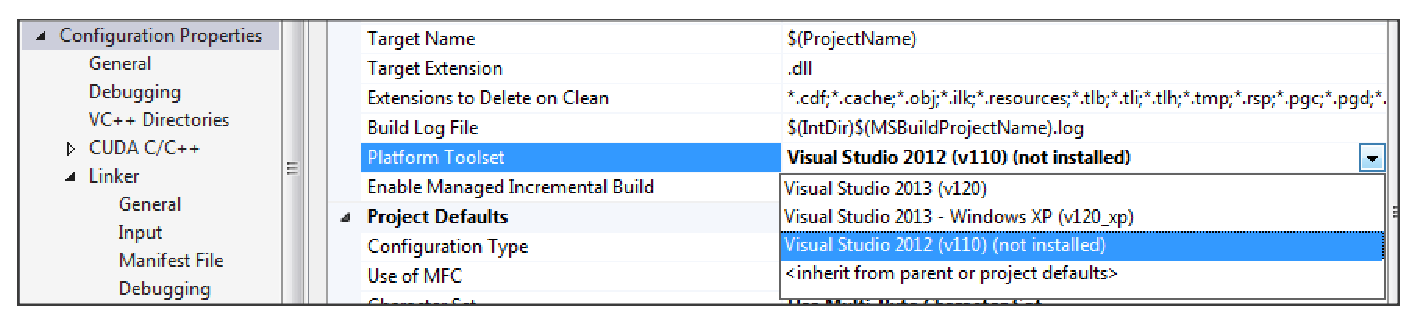
\includegraphics[height=2.7cm,
    angle=0]{./images/MSBuild_platform-toolset.eps}}
\caption{MSBuild platform toolset}
\label{fig:MSBuild_platform-toolset}
\end{figure}


\subsection{Predefined Properties}

MSBuild uses a set of predefined properties (macros) to store information about
the project file and the MSBuild binaries.
\footnote{\url{http://msdn.microsoft.com/en-us/library/ms164309.aspx}}
\begin{verbatim}

MSBuildThisFileFullPath            return the fullpath to the current (.targets)
                                   file, e.g. CUDA 6.0.targets
MSBuildThisFileExtension

MSBuildThisFileName

MSBuildToolsPath				  (cannot be overridden) the installation path of the
                                  MSBuild version that is associated with the
                                  value being chosen in MSBuildToolsVersion
      32-bit MSBuild 12.0+ : %ProgramFiles%\MSBuild\12.0\bin
      64-bit MSBuild 12.0+ : %ProgramFiles%\MSBuild\12.0\bin\amd64 
                                  
MSBuildToolsVersion                                                 
\end{verbatim}

\subsection{.props (property sheet)}

There are multiple property groups (import groups) instead of one. This allows
the last definition overrides the preceding ones.

\begin{verbatim}
<Import Project="$(VCTargetsPath)\Microsoft.Cpp.Default.props" />

<Import Project="$(VCTargetsPath)\Microsoft.Cpp.props" />

 <ImportGroup Label="ExtensionSettings">
    <Import Project="CUDA 6.0.props" />
  </ImportGroup>
  
  <ImportGroup Condition="'$(Configuration)|$(Platform)'=='Release|x64'" Label="PropertySheets">
    <Import Project="$(UserRootDir)\Microsoft.Cpp.$(Platform).user.props" Condition="exists('$(UserRootDir)\Microsoft.Cpp.$(Platform).user.props')" Label="LocalAppDataPlatform" />
  </ImportGroup>  
\end{verbatim}

\begin{enumerate}
  \item Default settings for a VC++ Project (not tool-specific), i.e.
  definitions for properties like Platform, PlatformToolset, OutputPath, TargetName, UseOfAtl,
  etc.
\begin{verbatim}
Import Project="$(VCTargetsPath)\Microsoft.Cpp.default.props" />
\end{verbatim}  

  \item Default values for many tool-specific properties, e.g. compiler's
  Optimization, WarningLevel properties, Midl tool's TypeLibraryName property,
  etc.
\begin{verbatim}
<Import Project="$(VCTargetsPath)\Microsoft.Cpp.props" />
\end{verbatim}
\end{enumerate}


Example:
\begin{verbatim}
<Project DefaultTargets="Build" ToolsVersion="4.0" xmlns='http://schemas.microsoft.com/developer/msbuild/2003' >
  <ItemGroup Label="ProjectConfigurations" />
  <PropertyGroup Label="Globals" />
  <Import Project="$(VCTargetsPath)\Microsoft.Cpp.default.props" />
  <PropertyGroup Label="Configuration" />
  <Import Project="$(VCTargetsPath)\Microsoft.Cpp.props" />
  <ImportGroup Label="ExtensionSettings" />
  <ImportGroup Label="PropertySheets" />
  <PropertyGroup Label="UserMacros" />
  <PropertyGroup />
  <ItemDefinitionGroup />
  <ItemGroup />
  <Import Project="$(VCTargetsPath)\Microsoft.Cpp.targets" />
  <ImportGroup Label="ExtensionTargets" />
</Project>
\end{verbatim}

\url{http://blogs.msdn.com/b/visualstudio/archive/2010/05/14/a-guide-to-vcxproj-and-props-file-structure.aspx}

\subsection{.targets}

There can be one or more \verb!.targets! files in your project. Each file
contains items, properties, targets, and tasks for common scenarios. These files
are typically automatically imported from somewhere else
\begin{itemize}
  \item Microsoft.CSharp.targets
  \item Microsoft.Common.targets
  \item Microsoft.VisualBasic.targets
  \item CUDA 6.0.targets
  \item CUDA 6.5.targets
\end{itemize}
Depending on the value of \verb!ToolsVersion!, the location is a subfolder of
\begin{verbatim}
<WindowsInstallationPath>\Microsoft.NET\Framework
\end{verbatim}
Example: ToolsVersion=4.0, then 
\begin{verbatim}
C:\Windows\Microsoft.NET\Framework\v4.0.30319
\end{verbatim}
The location of these file is defined in \verb!$(MSBuildToolsPath)!

If your project import one of these files, you will see this line in the Project
XML-based file
\begin{verbatim}
<Import Project="Microsoft.Common.targets" />
<Import Project="$(MSBuildToolsPath)\Microsoft.CSharp.targets" />
<Import Project="$(MSBuildToolsPath)\Microsoft.VisualBasic.targets" />
\end{verbatim}



\begin{verbatim}
http://msdn.microsoft.com/en-us/library/ms164312.aspx
\end{verbatim}

\subsection{MSBuild 4.5}

In VS 2012, MSBuild version number is 4.5 with .NET framework 4.5. 

You can build app targets to 
\begin{itemize}
  \item ARM processor
  \item
  \url{http://msdn.microsoft.com/en-us/library/hh162058(v=vs.110).aspx}
\end{itemize}


\subsection{MSBuild 12.0}

Since Visual Studio 2013, MSBuild is part of Visual Studio,
rather than .NET framework (4.5.1), and thus is installed under
\begin{verbatim}
C:\Program Files\MSBuild\.
\end{verbatim}
Also, the version number jumps to (version 12.0).


\url{http://msdn.microsoft.com/en-us/library/hh162058(v=vs.121).aspx}



\subsection{Build CUDA code in VS}

When adding CUDA acceleration to existing applications, the relevant Visual
Studio project files must be updated to include CUDA build customizations.
If you create a new project, remember to select
\begin{verbatim}
File-> New | Project... NVIDIA-> CUDA->
\end{verbatim}
and finally select a template for CUDA toolkit version, e.g. CUDA 6.5. runtime
template.  The new project is technically a C++ project (.vcxproj) that is
preconfigured to use NVIDIA's Build Customizations. 
So, all standard capabilities of Visual Studio C++ projects will be available.
If the location of CUDA toolkit is not standard, then under {\bf CUDA C/C++},
select {\bf Common}, select {\bf CUDA Toolkit Custom Dir}, and type the location
of the CUDA toolkit (you can use \verb!$(CUDA_PATH)! to use the latest
CUDA toolkit version).

If you have an existing project/solution and you want to add CUDA code.
To build CUDA code in Visual Studio, we need to define Custom Build Rules (or
Build Customization), which has already been defined by NVidia, you just need to
tell where the files are
\begin{enumerate}
  \item There are some additional settings you need to do, if you don't
  have Nvidia Nsight. From your project, select Custom Build Rules, select Find
  Existing. Browser to
\begin{verbatim}
C:\Program Files\NVIDIA Corporation\NVIDIA GPU Computing SDK\C
\end{verbatim}
and select CUDA.rules. This add two files (.targets and .props)

   \item Go to Project / Custom Build Rule (later changed to {\bf Build
   Customization}), and select the right CUDA toolkit version
   \footnote{\url{http://blogs.msdn.com/b/visualstudio/archive/2010/04/26/custom-build-steps-tools-and-events.aspx}}
\begin{verbatim}
``Enable CUDA rule''

CUDA 3.1 (.targets, .props)
CUDA 3.2 (.targets, .props)
CUDA 6.0 (.targets, .props)
CUDA 6.5 (.targets, .props)
\end{verbatim}
\url{http://blog.cuvilib.com/2011/02/24/how-to-run-cuda-in-visual-studio-2010/}

   \item You can also configure to use the latest version of CUDA toolkit
   (whose path is given in \verb!$(CUDA_PATH)! environment variable), by opening
   the Project's Properties page, Under CUDA C/C++, select Common, and set the
   CUDA Toolkit Custom Dir field.
\end{enumerate}

Select Include files:
\begin{itemize}
  \item Click Tools / Options / Project and Solutions / VC++ Directories
  \item Specify Include, then show the Directories
  \item For each line below, click 'New' and add them 
\begin{verbatim}
C:\Program Files\NVIDIA Corporation\CUDA\include

C:\Program Files\NVIDIA Corporation\NVIDIA GPU Computing SDK\C\common\inc
\end{verbatim}
\end{itemize} 


Select Lib files
\begin{itemize}
  \item Do the same, sepecify Lib
\begin{verbatim}
C:\Program Files\NVIDIA Corporation\NVIDIA GPU Computing SDK\C\common\lib

C:\Program Files\NVIDIA Corporation\CUDA\lib64
\end{verbatim}  
\end{itemize}

Select the executable files
\begin{itemize}
  \item Do the same, specify the executables
\begin{verbatim}
C:\Program Files\NVIDIA Corporation\CUDA\bin64
\end{verbatim}
\end{itemize}


Select the Linker options
\begin{verbatim}
Project -> Properties  -> Linker -> Input
 -> Additional Dependencies
\end{verbatim}
add 
\begin{verbatim}
cudart.lib
cutil64D.lib
\end{verbatim}
then
\begin{verbatim}
Project -> Properties  -> Linker -> General

and add path
C:\Program Files\NVIDIA Corporation\NVIDIA GPU Computing SDK\C\common\lib

C:\Program Files\NVIDIA Corporation\CUDA\lib64
\end{verbatim}

Increase the stack Reserve size
\begin{verbatim}
Project -> Properties ->
     Linker -> System -> Stack Reserve Size=500000000
\end{verbatim}

Now you can add your CUDA (.cu) source code. 

The last step is to specify the location where to put the output file (which
can be executable file or dynamic-link library DLL). Here, we use Project's
Property page $\rightarrow$ Linker, and modify \verb!Output File! textbox


In order to debug the CUDA code, you need to copy necessary CUDA library files
to the \verb!$(Outdir)! folder where the binary file is created. You can do this
by using Post-Build Event (Sect.\ref{sec:MSBuild_Events})
\begin{verbatim}
copy "$(CudaToolkitBinDir)\cudart*.dll" "$(OutDir)"
copy "$(CudaToolkitBinDir)\curand*.dll" "$(OutDir)"
\end{verbatim}
or you can get the error
\begin{verbatim}
The program can't start because cudart32_50_35.dll is missing from your
computer.
\end{verbatim}




\subsection{Build CUDA source code examples}

CUDA examples are stored in
\begin{verbatim}
%% Windows XP
C:\Documents and Settings\All Users\Application Data\NVIDIA Corporation\CUDA
Samples\v6.5

%% (newer)
C:\ProgramData\NVIDIA Corporation\CUDA Samples\v6.5
\end{verbatim}
\verb!C:\ProgramData! is a hidden folder.

Open the solution files from
\begin{verbatim}
C:\ProgramData\NVIDIA Corporation\CUDA Samples\v6.5\<category>\<sample_name>
\end{verbatim}
or the global solution files
\begin{verbatim}
C:\ProgramData\NVIDIA Corporation\CUDA Samples\v6.5
\end{verbatim}

From CUDA 6.x, CUDA samples are organized in categories
\begin{verbatim}
0_Simple
1_Utilities
2_Graphics
3_Imaging
4_Finance
5_Simulations
6_Advanced
7_CUDALibraries
\end{verbatim}

The environment variables are set automatically using the Buidl Customization 
\begin{verbatim}
CUDA 6.5.props
\end{verbatim}
which is installed as part of CUDA 6.5 toolkit. Location of this file

\begin{verbatim}
%% VS 2010
C:\Program Files (x86)\MSBuild\Microsoft.Cpp\v4.0\V100\BuildCustomizations

%% VS 2012
C:\Program Files (x86)\MSBuild\Microsoft.Cpp\v4.0\V110\BuildCustomizations

%% VS 2013
C:\Program Files (x86)\MSBuild\Microsoft.Cpp\v4.0\V120\BuildCustomizations
\end{verbatim}

The sample projects also use \verb!$(CUDA_PATH)! to detect the necessary files.

\subsection{Build CUDA code with a different CUDA toolkit version without
changing the Project's files}

In the command line, switch to the project's folder, and run
\begin{verbatim}
msbuild <projectname.extension> /t:Rebuild
    /p:CudaToolkitDir="drive:/path/to/new/toolkit/"
\end{verbatim}


\url{http://docs.nvidia.com/cuda/cuda-getting-started-guide-for-microsoft-windows/index.html#axzz3Fd0ryRW3}



\subsection{Build to 64-bit}

Solution / Configuration Manager / Active Solution Platform = New; select
\verb!x64! and import settings from win32.

Make sure Project / Properties / Linker / Advanced / Target Machine = x64

\subsection{Build a DLL}

You may need a module-definition (.def) file which 
 provide the linker with information about exports, attributes, and other
information about the program to be linked.

\begin{verbatim}
Project's Property
   --> LInker
      --> Input
          --> Module Definition File 
                    CUDAFluxEngine.def
\end{verbatim}

In that file, we specify which APIs are exported to use, or we can do explicitly
inside the code with
\begin{verbatim}
__declspec(dllexport) 
\end{verbatim}
as a way to specify exported functions.

\url{http://msdn.microsoft.com/en-us/library/28d6s79h.aspx}

\subsection{Build Events}
\label{sec:MSBuild_Events}

You can specify what to do before or after the build using
\begin{verbatim}
Project's Property
   --> Build Events
       --> Pre-Build Event
           Pre-Link Event
           Post-Build Event
\end{verbatim}

These are indeed batch files. The utility \verb!COMMAND.COM! read one line
from the batch file, execute command, and repeat the process (reading next
line from the file, execute that line). This applies to comment line as well,
i.e. each comment line causes one extra re-read of the batch file. To indicate
a comment line, it use REM (REMarks) to start a comment line.
\url{http://www.robvanderwoude.com/comments.php}

To put the comments or temporarily comment out a command, we put \verb!REM! in
the front
\begin{verbatim}
REM signtool sign /a $(TargetPath) xcopy /Y "$(TargetPath)" "C:\Deploy\$(TargetFileName)"
\end{verbatim}
\url{http://stackoverflow.com/questions/5626166/proper-way-to-put-comments-in-build-events-command-line}

\subsection{Build Linker}

Here, you specify where to put the output file which can be an executable file
or a dynamic-link library.

Make sure that
\begin{verbatim}
$(OutDir), $(TargetName) and $(TargetExt) 
\end{verbatim}
property values match the value specified in \verb!%(Link.OutputFile)!.

To specify additional dependencies, use
\begin{verbatim}
Project's Property
   --> LInker
      --> Input
        --> Additional Dependencies
                  ann.lib;nvapi64.lib;cudart.lib;curand.lib;
\end{verbatim}

\url{http://msdn.microsoft.com/en-us/library/y0zzbyt4.aspx}

NOTE:
\begin{verbatim}
/LTCG specified but no code generation required; remove /LTCG from the link
command line to improve linker performance
\end{verbatim}


\subsection{Build some projects in a solution}	


You can do this from the command-line
\begin{verbatim}
msbuild /P:Configuration=Release PACKAGE.vcxproj
\end{verbatim}
or using Visual Studio: right-click on Solution page, and select {\bf
Configuration Manager}.

You may get the error
\begin{verbatim}
warning MSB3270: There was a mismatch between the processor architecture of the
project being built "MSIL" and the processor architecture of the reference "DocumentServiceModel", "x86".
\end{verbatim}
if some projects in the same solution has a conflict built target between them.

If your solution have multiple projects and some of them are just libraries;
then if you select to debug, you may get the error
\begin{verbatim}
A project with an Output type of Class Library cannot be started directly
\end{verbatim}
To fix this, right click Solution's Property page
\begin{verbatim}
--> Common Properties --> Startup Project
\end{verbatim}
you can choose either below, but just to make sure the project you run is not
the one compiled into the library
\begin{itemize}
  \item Current selection
  \item Single startup project
  \item Multiple startup projects
\end{itemize}

\section{NAnt}
\label{sec:NAnt}

NAnt is used to automate builds.
NAnt 0.92 only supports .NET 4.0

\section{CUDA in Windows}

In order to program CUDA in Windows, you need
\begin{enumerate}
  \item CUDA-capable GPU
  \item a supported version of Windows
  \item a supported version of IDE, e.g. Visual Studio
  \item NVIDIA CUDA Toolkit (which include the driver as well)
  
Example: command line in silent mode  
\begin{verbatim}
<PackageName>.exe -s CUDAToolkit_6.5 Display.Driver
\end{verbatim}  
\end{enumerate}


The default installation location is
\begin{verbatim}

%% Toolkit
C:\Program Files\NVIDIA GPU Computing Toolkit\CUDA\v6.0

C:\Program Files\NVIDIA GPU Computing Toolkit\CUDA\v6.5


%% Samples  (hidden folder)
C:\ProgramData\NVIDIA Corporation\CUDA Samples\v6.0


%% Documentation

\end{verbatim}

There are two driver model can be used on Windows 7 and later
\begin{enumerate}
  \item WDDM: used for display devices
  \item Windows WDM: available for non-display device and Nvidia driver mode TCC
  (Tesla Compute Cluster) uses this. This is not supported in GeForce family.
  Advantages:
  \begin{itemize}
    \item use CUDA with Windows Remote Desktop
    \item use CUDA within processes running as Windows Services
    \item reduce latency in CUDA kernel launches + eliminate timeouts that can
    occur when running under WDDM due to Windows TDR
    \footnote{\url{http://msdn.microsoft.com/en-us/library/windows/hardware/ff570087(v=vs.85).aspx}}
  \end{itemize}
\end{enumerate}
TCC is enabled by default on most recent GPUs (and condition: it must not be
used for display), we can check with
\begin{verbatim}
nvidia-smi
\end{verbatim}

\subsection{Syntax hightlighting}


Visual Studio / Tools / Options / text Editor / File Extension.
\begin{verbatim}
Tools | Options | Projects | VC++ Build | C/C++ File Extensions (VS.NET)

Tools | Options | Projects and Solutions | VC++ Project Settings | C/C++ File Extensions (VS2005, VS2008)

Tools | Options | Projects and Solutions | VC++ Project Settings | Extensions To Include (VS2010)
\end{verbatim}

Then add \verb!cu!, \verb!cuh! to Microsoft Visual C++.
\url{http://stackoverflow.com/questions/14827160/how-do-i-enable-syntax-highlighting-of-cuda-cu-files-in-visual-studio-2010}

If you use Visual Studio 2012 or older, please continue the below steps.
To avoid syntax highlighting of CUDA keywords (like threadldx.x), we need to
include in the CUDA code (so that IDE won't show false syntax errors)
\begin{verbatim}
#include<device_launch_parameters.h>
\end{verbatim}
However, using this may cause \verb!nvcc!'s intrinsic compiler functions for arithmetic
to appear undefined if you have both
\begin{verbatim}
#include "cuda_runtime.h"
#include "device_launch_parameters.h"
\end{verbatim}
The fix is to remove those two includes from the project when you want to
compile.
\url{http://stackoverflow.com/questions/13966469/why-dont-the-cuda-compiler-intrinsics-fadd-rd-etc-work-for-me}

You may use \verb!usertype.dat! in (until CUDA 5.0)
\begin{verbatim}
C:\ProgramData\NVIDIA Corporation\CUDA
Samples\v5.0\doc\syntax_highlighting\visual_studio_8
\end{verbatim}
copy the content and append to the same file name (if existing) or copy (if the
file is not in the below folder) in the below folder
\begin{verbatim}

%% VS 2012 is being used
C:\Program Files\Microsoft Visual Studio 12.0\Common7\IDE
\end{verbatim}

Finally, restart the Visual studio

NOTE: Example of the usertype.dat file content
\begin{verbatim}
__global__
__host__
__device__
__constant__
__shared__
gridDim
blockIdx
blockDim
threadIdx
int1
uint1
int2
uint2
int3
uint3
int4
uint4
float1
float2
float3
float4
char1
char2
char3
char4
uchar1
uchar2
uchar3
uchar4
short1
short2
short3
short4
dim1
dim2
dim3
dim4
tex1D
tex1Dfetch
tex2D
__float_as_int
__int_as_float
__float2int_rn
__float2int_rz
__float2int_ru
__float2int_rd
__float2uint_rn
__float2uint_rz
__float2uint_ru
__float2uint_rd
__int2float_rn
__int2float_rz
__int2float_ru
__int2float_rd
__uint2float_rn
__uint2float_rz
__uint2float_ru
__uint2float_rd
__fadd_rz
__fmul_rz
__fdividef
__mul24
__umul24
__mulhi
__umulhi
__mul64hi
__umul64hi
min
umin
fminf
fmin
max
umax
fmaxf
fmax
abs
fabsf
fabs
sqrtf
sqrt
sinf
__sinf
sin
cosf
__cosf
cos
sincosf
__sincosf
expf
__expf
exp
logf
__logf
log
__syncthreads
\end{verbatim}

\subsection{Relocatable code}

You can put CUDA code into header file (\verb!.cuh! or \verb!.h!) and
implementation in the source file (\verb!.cu!) by adding 

\begin{verbatim}
--relocatable-device-code=true
\end{verbatim}

\begin{verbatim}
View -> Property Pages; Configuration Properties -> 
   CUDA C/C++ -> Common ->
          Generate Relocatable Device Code 
             -> Yes (-rdc=true).
\end{verbatim}

Otherwise, we can get the error
\begin{verbatim}
Error   19  error : Unresolved extern function '_ZN16LibraryNameSpace5int2_aSEi'
      C:\Users\Documents\Project\Test\Testing_Files\ptxas simpleTest
\end{verbatim}

\url{http://stackoverflow.com/questions/17188527/cuda-external-class-linkage-and-unresolved-extern-function-in-ptxas-file}

\subsection{CUDA 3.2}

CUDA 3.2 only supports upto Visual Studio 2008 (Sect.\ref{sec:VS_2008}).

To run CUDA 3.2 code on newer Visual Studio, you also need to have Visual Studio
2008 installed or at least a VC90 C compiler on the machine with the appropriate
Windows SDK.
\begin{verbatim}
Visual Studio 2008
Windows SDK v6.0A
\end{verbatim}
The reason is that CUDA Toolkit 3.2 does not has support for the
VS100 C compiler.

Now the reason why you need to have NSight installed. Without NSight, you will
have to manually specify the CUDA properties and target files so in order to
avoid that, better download and install NSight. Make sure you enable NSight for
both VS 2008 and VS 2010. Now we're ready to roll!

\subsection{CUDA 5.0}

\url{https://code.msdn.microsoft.com/windowsdesktop/CUDA-50-and-Visual-Studio-20e71aa1}


\subsection{CUDA 5.5}

CUDA 5.5 fully supports Visual Studio 2012.

\subsection{CUDA 6.0}

CUDA 6.0 only works with Microsoft Visual Studio 2012.

\subsection{CUDA 6.5}

CUDA 6.5RC officially supports Microsoft Visual Studio 2013.

\begin{itemize}
  \item Building native x86-32 is deprecated, i.e. choose either native x86-64
  or cross (x86-32 binary on x86-64 O/S). However, building native x86-64 is not
  supported using VS Express 2013 for Windows Desktop.
  
  \item No support for Windows XP (32 or 64)
  \item support VS13 (compiler VC++ 12) but not VS Express 2013 for Windows,
  VS12 (compiler VC++ 11), VS10 (compiler VC++ 10)
  
  \item New hardware support: ARM64
\end{itemize}

\section{Microsoft Management Console (MMC)}


MMC = Microsoft Management Console, a component of Windows 2000 that provide
system administrator (and advanced users) an interface to configure and monitor
the system.

To create an application that use MMC, you create an MMC {\it snap-ins}, i.e. a
COM component, which is then registerred in
\begin{verbatim}
[HKEY_CLASSES_ROOT]\{CLSID} and
[HKEY_LOCAL_MACHINE\Software\Microsoft\MMC\Snapins]
\end{verbatim}

Compared to traditional GUI apps, an MMC snap-ins can be loaded remotely to
control some server application. Other pros and cons
\footnote{\url{http://stackoverflow.com/questions/473306/benefits-of-developing-mmc-snap-ins-instead-of-traditional-gui-apps}}
\begin{itemize}
  \item PROS
  \begin{enumerate}
    \item standard UI with sys-admins
    \item treeview + listview model, with classes for implementing element
    properties, selection, context menus, column selection, etc.
    \item good for quick, small configuration interface
  \end{enumerate}
  \item CONS
  \begin{enumerate}
    \item not flexible (e.g. no way to change background color)
    \item no source code, i.e. hard to deal with threading
    \item poor documentation
    \item not a good choice if you want something more complicated
  \end{enumerate}
\end{itemize}

A snap-ins combine with MMC is called a {\it console}, which can be launched by
users using
\begin{verbatim}
mmc path \ filename.msc [/a] [/64] [/32]
\end{verbatim}

Example: \url{http://www.codeproject.com/Articles/2587/Developing-MMC-Snap-ins}


% \section{Using an existing component (.DLL)}
% 
% You can write some components from that you can add to use in another project.
% The component can be compiled into DLL. Then from your project, you add
% {\bf reference} to it.
% 


\section{.NET application: Assembly}

An assembly is a file, automatically generated by the compiler upon a successful
compilation a .NET application. This file can be either a DLL or an executable
file.

An assembly contains IL code (Intermediate Language), similar to Java byte code.
There are two kinds of assembly: {\bf Single file} or {\bf Multi file}.
\begin{itemize}
  \item Single file assembly: contains all the required information (Metada,
  Manifest) in a single package
  \item Multi file assembly: two or more .NET binaries or modules.
\end{itemize}

The goal of using assembly is to enable integrating code written in different
language in the .NET framework.

\url{http://www.codeguru.com/columns/csharp_learning/article.php/c5845/C-FAQ-15--What-is-an-Assembly.htm}



\section{Configuration Properties}
\label{sec:VS_Configuration_Properties}

\subsection{Add header file}

Global-level setting: (until Visual Studio 2008)
\begin{verbatim}
Visual Studio 'Tools' menu
  Options ...
     
click Projects and Solutions
  VC++ Directories ...
     for each Platform
        choose the location for the "Include files"
\end{verbatim}
VS 2008 VC++ Directories were per-user, per-machine and made SCC enlistments
fragile.  VS 2008 VC++ Directories were applied to all projects loaded on that
machine and could not be stopped. This causes problems when working with multiple projects in a solution.
\url{http://blogs.msdn.com/b/vsproject/archive/2009/07/07/vc-directories.aspx}

There is a major change in \verb!VC++ Directories! setting from VS2008 to
VS2010.  Since VS2010, \verb!VC++ Directories! setting is moved to per project
setting.
Using the project properties window, there are two ways of adding the include
directories
\begin{enumerate}
  \item VC++ Directories and \verb!Include Directories!
  

%Since VS2010: the edits are NOT per-user, per-machine as they were in VS 2008. 
  
  \item C/C++ and \verb!Additional Include Directories!
  
\end{enumerate}
\url{http://stackoverflow.com/questions/1124381/what-is-the-diff-b-w-includes-in-vc-directories-options-and-additional-include}

\subsection{Add references to .LIB library (static library or import library)}

The best way is to add reference to the original project file, if the .LIB
project is in the same solution with the project that use the library.
Therefore, Visual Studio can take care of copying and linking the library each
time it is recompiled.

If the library is from a third-party product, i.e. you have no access to the
source code, but you have the header files and .LIB file, 
then there are three ways to link a static library or import library to your project
in Visual Studio

\begin{enumerate} 
  \item Global level (until Visual Studio 2008): done once for a library (\textcolor{red}{This option is
  obsolete since Visual Studio 2010 as it is considered better to configure at
  project's level only})

The setting will be applied for all projects and solutions
\begin{verbatim}
Visual Studio 'Tools' menu
  Options ...
     
click Projects and Solutions
  VC++ Directories ...
     for each Platform
        choose the location for the "Include files"
            and "Library files" 
\end{verbatim}
  
  \item Project level (recommended for third-party library): done once for a project and a library 

We need to add (1) the library search path, (2) the library filenames. We can specify them separately or at once. 

There are two ways to specify the library search path
\begin{itemize}
  \item Configuration Properties / VC++ Directories, select \verb!Library Directories! and add your \verb!*.lib! path
  
  \item Configuration Properties / Linker, select \verb!Additional Library Directories!, and add your \verb!*.lib! path 
\end{itemize}

Then we add the library filenames
\begin{verbatim}
right-click  Project's properties
  select Configuration: All Configurations
     
Configuration Properties
    Linker
       Input
       
Use "Additional Dependencies"
  add the name of the .LIB library
  
         
\end{verbatim}  

We don't need to specify the library search path if we put the relative path as well as the library filename in the 
\verb!Additional Dependencies! section above.
\begin{verbatim}
.\Lib\mystatic.lib
\end{verbatim}
rather than just 
\begin{verbatim}
mystatic.lib
\end{verbatim}
  
  
   \item Project-leve: drag-and-drop the library to
   the project, put in the \verb!Resource Files! folder. Then, in your code, either   
\begin{itemize}
  \item add the reference to header files of the third-party library
  \item add an \verb!extern! reference defining the funciton you want to use before calling the third-party function. 
\end{itemize}
\url{http://www.codeproject.com/Articles/85391/Microsoft-Visual-C-Static-and-Dynamic-Libraries}

  
  \item File level (only work with Visual Studio): done once for a project and a library and a file using \verb!#pragma!
  
\begin{verbatim}
#include "curses.h"

#pragma comment(lib, "PDCurses.lib")
\end{verbatim}
   
\end{enumerate}
\url{http://www.learncpp.com/cpp-tutorial/a2-using-libraries-with-visual-studio-2005-express/}

% If your code using an external library (*.lib, *.dll), there are three ways to add the reference to it
% \begin{enumerate}
% %   Then, add the name of the library file in Configuration Properties / Linker / Input. 
% %   
% %   Then, add the name of the library file in Configuration Properties / Linker / Input.
%   
%   \item  Configuration Properties / Linker, select Additional Library Directories, and add your \verb!*.lib! path along with the library filename. Here, the exact filename full path is used. 
%   
% \end{enumerate} 
\url{https://social.msdn.microsoft.com/Forums/vstudio/en-US/6fa1b12d-95e1-4ecf-bca2-ed2dc8594dd4/additional-lib-path-in-vc-directories-or-in-linker-general?forum=vcgeneral}

\subsection{C++ code add references to .DLL library}

{\bf Scenario 1}: (you own the DLL source) The best way is to add reference to
the original project file, if the .DLL project is in the same solution with the
project that use the library.
Therefore, Visual Studio can take care of copying and linking the library each
time it is recompiled.

{\bf Scenario 2:} If the library is from a third-party product, i.e. you have no
access to the source code, but you have the header files and both the .LIB and
.DLL file, then you use the so-called {\bf implicit linking} (the machine code
is known as compile time, but not actually included in the final application).
\begin{enumerate}
  \item put the .LIB file into \verb!Resource Files!
  \item use \verb!__declspec(dllimport)! in the code
    
\end{enumerate}
Example: in Project explorer
\begin{verbatim}
Header files
  add.h
Resource Files
  add.lib
  
Source files
  main.cpp
\end{verbatim}
%need (1) add reference to the DLL, (2) modify the header file to use

{\bf Scenario 3}: If the library is from a third-party product, i.e. you have no
access to the source code, but you have the header files and .LIB and .DLL file, then you

\begin{enumerate}
  \item add reference to the .LIB file
  
From Project's page, right-click
\begin{verbatim}
 --> Add References ... (VS 2010 and older)
 
 --> Add --> References ...  (VS 2012 and newer)
 
\end{verbatim}
  
  
   \item Tell the compiler that the function to be used is from a DLL library: there are two options
   \begin{enumerate}
     \item use \verb!__declspec(dllimport)! on the function declaration
\begin{verbatim}
#include <stdio.h>
#include "add.h"   // original add.h

extern int __declspec(dllimport) add(int a, int b);
int main() {
    int a = 2;
    int b = 1;
    printf("a=%d, b=%d\n", a,b);
    printf("add: %d\n", add(a,b));
    getchar();
    return 0;
}
\end{verbatim}  
     
   \item The original header file for the DLL project which has \verb!__declspec(dllexport)!, when copied to the
   project that uses the DLL, need to be modified so that the project know which API will be used

Example: modified add.h header file
\begin{verbatim}
#ifndef ADD_H
#define ADD_H
int __declspec(dllimport) add(int a, int b);
#endif  // ADD_H
\end{verbatim}

and then we use it
\begin{verbatim}
#include <stdio.h>
#include "add.h"   // modified add.h

int main() {
    int a = 2;
    int b = 1;
    printf("a=%d, b=%d\n", a,b);
    printf("add: %d\n", add(a,b));
    getchar();
    return 0;
}
\end{verbatim}

NOTE: This tells the compiler that this is referencing a dynamic library.
\begin{verbatim}
 __declspec(dllimport)
\end{verbatim} 
 
 
{\bf TIPS:} reusing the header file, i.e. no need to modify by defining a compiling flag
\verb!BUILD_DLL! (if on, the header file is used for building DLL; if off, the header file is used for linking the DLL), and 
thus define a simple macro \verb!PORT_DLL! that map to either \verb!__declspec(dllexport)! or \verb!__declspec(dllimport)! in the appropriate case.
Then, in Visual Studio's project, add \verb!/D ``BUILD_DLL''! to additional options (Sect.\ref{sec:VS_Configuration_Properties_command-line})
 
\begin{verbatim}
#ifndef ADD_H
#define ADD_H
#ifdef BUILD_DLL
#define PORT_DLL __declspec(dllexport)
#else
#define PORT_DLL __declspec(dllimport)
#endif
int PORT_DLL add(int a, int b);
#endif  // ADD_H
\end{verbatim}
 
 
 \end{enumerate}
 
 

\end{enumerate}


You can modify this in the project (.csproj) file

Example: 
\begin{verbatim}
  <ItemGroup>
    <Reference Include="DockContainer, Version=1.2.0.0, Culture=neutral, PublicKeyToken=6ca3e369254a63c5, processorArchitecture=MSIL">
      <SpecificVersion>False</SpecificVersion>
      <HintPath>..\..\..\CUDAflux\DLLs\DockContainer.dll</HintPath>
    </Reference>
    <Reference Include="SolarClasses, Version=1.0.4113.17144, Culture=neutral, PublicKeyToken=6ca3e369254a63c5, processorArchitecture=MSIL">
      <SpecificVersion>False</SpecificVersion>
      <HintPath>..\..\..\CUDAflux\DLLs\SolarClasses.dll</HintPath>
    </Reference>
    <Reference Include="System" />
    <Reference Include="System.Core">
      <RequiredTargetFramework>3.5</RequiredTargetFramework>
    </Reference>
    <Reference Include="System.Data" />
    <Reference Include="System.Data.DataSetExtensions">
      <RequiredTargetFramework>3.5</RequiredTargetFramework>
    </Reference>
    <Reference Include="System.Deployment" />
    <Reference Include="System.Drawing" />
    <Reference Include="System.Runtime.Serialization" />
    <Reference Include="System.ServiceModel" />
    <Reference Include="System.ServiceModel.Discovery" />
    <Reference Include="System.Transactions" />
    <Reference Include="System.Windows.Forms" />
    <Reference Include="System.Windows.Forms.DataVisualization" />
    <Reference Include="System.Xml" />
  </ItemGroup>
\end{verbatim}

\subsection{Command-line}
\label{sec:VS_Configuration_Properties_command-line}

Choose Project's properties
\begin{verbatim}
Configuration: All Configurations

Configuration Properties
   C/C++
      Command Line
         Additional Options
\end{verbatim}


\subsubsection{System}
\label{sec:configuration-properties_Linker_subsystem}

\verb!SubSystem! option (if it does not appear, make sure you change the
configuration manager to use x64, rather than Win32) has a number of values

\begin{verbatim}
Not Set
Console (/SUBSYSTEM:CONSOLE)
Windows (/SUBSYSTEM:WINDOWS)
Native (/SUBSYSTEM:NATIVE)
EFI Application (/SUBSYSTEM:EFI_APPLICATION)
EFI Boot Service Driver (/SUBSYSTEM:EFI_BOOT_SERVICE_DRIVER)
EFI Rom (/SUBSYSTEM:EFI_ROM)
EFI Runtime Driver (/SUBSYSTEM:EFI_RUNTIME_DRIVER)
POSIX (/SUBSYSTEM:POSIX)
\end{verbatim}

\subsubsection{Advanced}

We can select a specific funciton as the entry point. This is particularly
useful when developping Windows Form application (to run on CLR) where the name
of the entry function is different from the default \verb!main()! function in
Visual C++.

Example: the name is \verb!Main()! 
\begin{verbatim}
Main
\end{verbatim}


\section{Windows Runtime ABI}
\label{sec:Windows-Runtime-ABI}

\url{http://blogs.msdn.com/b/vcblog/archive/2012/08/30/cxxcxpart00anintroduction.aspx}

\section{Windows Store apps}
\label{sec:Windows-store-apps}

C++ Windows Store apps use XAML (Sect.\ref{sec:XAML}) to define the user
interface, and use native stack. 

\url{http://msdn.microsoft.com/en-us/library/hh699871.aspx}

\section{Visual C++ Linker best practices}
\label{sec:Linker_VisualC++}

To know how much time the spent for linking during the code compilation phase,
we can add \verb!/time! flag to the linker command line
\begin{verbatim}
// VC++
Project properties
   Configuration Properties 
       C++
           Command Line: add /time

// CUDA
Project properties
   Configuration Properties
      Linker
         Command Line: add /time             
\end{verbatim}


\begin{verbatim}
// VC++
Project properties
   Configuration Properties 
       C++
           Command Line: add /time

\end{verbatim}

Now, we learn how to link incrementally. When linking incrementally, the linker
directly updates the binaries produced on the previous link rather than building
them from scratch.  In addition to incrementally updating the binary, the linker
incrementally updates the corresponding PDB as well.
 To enable the ability to add code to an existing binary on subsequent links,
the linker inserts extra padding into a binary as it's being built. As a result,
a binary built with incremental linking enabled will be larger than a binary
built without incremental linking.  \textcolor{red}{In the developer iteration
scenario, the additional size is generally accepted as a fair tradeoff for
faster link times.} However, larger binaries will take longer to deploy on
remote hosts so you'll want to verify whether this tradeoff is acceptable in
your particular scenario. 

The \verb!/verbose:incr! switch will print various diagnostic messages you can
use to determine when the linker had to abandon incremental linking and fall back to a
full link. If a full link is done, it prints out
\begin{verbatim}
LINK : library changed; performing full link
\end{verbatim}

If you want to use incremental linking, then continue reading.
\begin{verbatim}
// CUDA
Project properties
   Configuration Properties
      Linker
         Enable Incremental Linking: Yes (/INCREMENTAL)
\end{verbatim}
/INCREMENTAL is on by default in the Debug configuration for projects created
using Visual Studio. Note also, that /INCREMENTAL is implied if you have
specified /DEBUG.


\url{http://blogs.msdn.com/b/vcblog/archive/2013/10/30/the-visual-c-linker-best-practices-developer-iteration.aspx}

\subsection{Force Symbol References}
\label{sec:Linker_ForceSymbolReferences}

Visual C++ projects support a linker property called
'Force Symbol References' which is accessed through the
property pages for the linker.

When this option is set, VS.NET generates additional /INCLUDE parameters to
the linker (link.exe).
\begin{itemize}
  \item 32-bit DLL:
\begin{verbatim}
ForceSymbolReferences="__DllMainCRTStartup@12"
\end{verbatim}

  \item 64-bit DLL:
  
\begin{verbatim}
ForceSymbolReferences="_DllMainCRTStartup"
\end{verbatim}
(one underscore and no trailing \verb!@12!)
\end{itemize}
NOTE: \verb!_DllMainCRTStartup! is the MFC entry point

\url{http://sourceforge.net/p/nant/bugs/356/}


\section{/MT, /MD}
\label{sec:/MT_/MD}

The compiling option /MT, /MD, and /LD specifies which version and which types
(single-threaded or multiple-threaded) of the C/C++ RunTime Libraries
(Sect.\ref{sec:CRT} and Sect.\ref{sec:C++_RT}) to use.

To compile your project to use a specific version of the multi-threaded
statically linked RunTime Library, we use \verb!/MT!
\begin{itemize}
  
  \item The application compiled with this option is statistically linked to
  \verb!mscvrt.lib!, but this lib is dynamically linked to a specific version of
  the RunTime Library DLL depending on the version of Visual Studio being used. 
  
  \item Two macros \verb!_MT! and \verb!_DLL! are defined automatically, which can be used to check in your code 
  to specify which code path to run 
\end{itemize}

To compile your project to use a specific version of the multi-threaded, dynamically linked 
Runtime Library, we use \verb!/MD!
\begin{itemize}
  \item The application compiled with this option is statistically linked to
  \verb!mscvrt.lib!, but this lib is dynamically linked to a specific version of
  the RunTime Library DLL depending on the version of Visual Studio being used. 

  \item 
\end{itemize}




DLL file, the DLL must be
compiled with \verb!/LD! or \verb!/LDd!, and then in your project, you pass
\verb!/DLL! option
\begin{verbatim}
/DLL "libname.dll"
\end{verbatim} 
The linker 

\section{Building DLL: /LD, /LDd }
\label{sec:building_DLL_/LD}

An explanation about DLL is given in Sect.\ref{sec:DLL}. In Visual Studio, to
build a DLL, you need to create a DLL project.
Behind the scence, the compiling option \verb!/LD! or \verb!/LDd! is used. In
Windows, an important concept is {\bf import library}
(Sect.\ref{sec:import_library}) which is a static library (.LIB) created during
the compilation of the DLL if the export file (*.exp) is not specified.


Unlike LIB, in DLL, by default, none of the symbols in a DLL is visible to
outside.  There is a number of ways to specify what symbols in a DLL are available to its users
\begin{enumerate}
  \item using .def file ({\bf module definition file}): is used to help create the .dll and
its import library .lib file.

In a .def file, you can specify what symbols in a DLL are available to its
users, and then the linker reads the information in .def and generates the .lib
import library file accordingly. 
  
NOTE: def was a must in early Win16 DLL programming, it is no longer necessary
to build a DLL in Win32 and thereafter.
  
   \item using \verb!__declspec(dllexport)! for the symbols in the source code
   
   \item using linker /EXPORT option to export a function on the LIB command (Sect.\ref{sec:LIB_command})
\begin{verbatim}
/EXPORT: entryname[= internalname][,@ ordinal[, NONAME]][, DATA]
\end{verbatim}   
\url{https://msdn.microsoft.com/en-us/library/0b9xe492.aspx}

\end{enumerate}

\textcolor{red}{SPECIAL CASE} (circular referencing): We need to build two executable files A.dll and B.dll, A use a
function in B, and B use a funciton in A. The problem is we cannot build any of
them using the above method, as in order to build A we need B and in order to
build B we need A. To resolve this problem, Microsoft introduced the concept of
an export file (*.exp).  When LIB creates an import library, it also creates an .exp file. 
Export (.exp) files contain information about exported functions and data items. 
So, the compilation works like a two-phase linking
\begin{itemize}
  \item phase 1: generate A.exp and B.exp
  \item phase 2: build A.dll use B.exp, and build B.dll use A.exp
\end{itemize}
In general the circular referencing is not a good idea, so hopefully you will not need .exp files in your project.
\url{http://binglongx.com/2008/10/01/dll-lib-def-and-exp-file-types/}

To build an import library and export file
\begin{verbatim}
LIB /DEF[:deffile] [options] [objfiles] [libraries]
\end{verbatim}
\url{https://msdn.microsoft.com/en-us/library/f0z8kac4.aspx}


Also, depending on whether the DLL needs to use
\begin{itemize}
  \item single-thread or multi-threaded
  \item statistically or dynamically-linked
\end{itemize}
version of the Runtime Library (Sect.\ref{sec:CRT} or Sect.\ref{sec:C++_RT}), an
appropriate compiling option need to be added as well (i.e. /ML[d], /MT, /MD) - Sect.\ref{sec:/MT_/MD}.


\section{/SUBSYSTEM}
\label{sec:/SUBSYSTEM}

The compiliing option /SUBSYSTEM:CONSOLE is for console based applications. The default entry point is 
\begin{itemize}
  \item \verb!main()! function native code
  \item \verb!wmain()! function native code
  \item \verb!int main(array^)! function C++/CLI code
\end{itemize}
NOTE: \verb!/SUBSYSTEM:CONSOLE! is the default for project build with \verb!/clr:safe! (Sect.\ref{sec:clr_option}).

The compiling option /SUBSYSTEM:WINDOWS is for an applications (not necessarily
GUI) without console, e.g. a service. The default entry point is 
\begin{itemize}
  \item \verb!WinMain()!
or \verb!wWinMain()! function for native code.
  \item C++/CLI code
\begin{verbatim}
WinMain(HISTANCE *, HINSTANCE *, char *, int) 

wWinMain(HINSTANCE *, HINSTANCE *, wchar_t *, int) 
\end{verbatim}
\end{itemize}

If you compile an application targetting Windows XP using MSVC 2013, 
use SUBSYSTEM:WINDOWS,5.1 (or :CONSOLE,5.1)

Program entry point is defined by /ENTRY linker option.

\section{\_\_stdcall vs. \_\_cdecl vs. \_\_thiscall vs. \_\_fastcall vs. \_\_vectorcall}

A calling convention is a way to define a function, that help the compiler to
follow the predefined rule on how to setup the stack, pushing arguments and
getting return value. This is not part of the C/C++ language specification, but is compiler extensions. 
\url{http://en.wikipedia.org/wiki/X86_calling_conventions}

\verb!__stdcall! is the calling convention used in Win32 APIs. This is how to
define a function following the same convention as Win32 API
\begin{verbatim}
return-type __stdcall function-name[(argument-list)]
\end{verbatim}
Example:
\begin{verbatim}
struct CMyClass {
   void __stdcall mymethod();
};

// Example of the __stdcall keyword on function pointer
typedef BOOL (__stdcall *funcname_ptr)(void * arg1, const char * arg2, DWORD flags, ...);
\end{verbatim}
\url{https://msdn.microsoft.com/en-us/library/zxk0tw93.aspx}

\url{http://www.codeproject.com/Articles/1388/Calling-Conventions-Demystified}

\section{WINAPI vs. APIENTRY}

WINAPI and APIENTRY both do pretty much the same thing (i.e. mapping to
\verb!__stdcall!). I prefer to use WINAPI for my executables and use APIENTRY
for the entry-point in DLLs

\begin{verbatim}
#define CALLBACK __stdcall
#define WINAPI __stdcall
#define WINAPIV __cdecl
#define APIENTRY WINAPI
#define APIPRIVATE __stdcall
#define PASCAL __stdcall
\end{verbatim}


\section{Utilities}

\subsection{DUMPBIN command}
\label{sec:dumpbin_command}


To check which version of Visual Studio was used to compiled the DLL.
\begin{verbatim}
dumpbin /imports <dllname.dll>
\end{verbatim}

Example: static library
\begin{verbatim}
D:\OpenSource\opencv_2.4.10\build\x64\vc12\staticlib>dumpbin opencv_calib3d2410.lib
Microsoft (R) COFF/PE Dumper Version 12.00.21005.1
Copyright (C) Microsoft Corporation.  All rights reserved.


Dump of file opencv_calib3d2410.lib

File Type: LIBRARY

  Summary

          20 .CRT$XCU
          37 .bss
          28 .data
         3EF .data$r
      20E480 .debug$S
         83C .debug$T
        3FC7 .drectve
        77C4 .pdata
        C6D2 .rdata
         A14 .rdata$r
          BD .text$di
       BA4B9 .text$mn
        F19B .text$x
          69 .text$yd
       22014 .xdata
\end{verbatim}


Example: import library
\begin{verbatim}
D:\OpenSource\opencv_2.4.10\build\x64\vc12\lib>dumpbin opencv_calib3d2410d.lib
Microsoft (R) COFF/PE Dumper Version 12.00.21005.1
Copyright (C) Microsoft Corporation.  All rights reserved.


Dump of file opencv_calib3d2410d.lib

File Type: LIBRARY

  Summary

          E7 .debug$S
          14 .idata$2
          14 .idata$3
           8 .idata$4
           8 .idata$5
          18 .idata$6
\end{verbatim}

Example:
\begin{verbatim}
D:\OpenSource\opencv_2.4.10\build\x64\vc12\bin>dumpbin opencv_calib3d2410.dll
Microsoft (R) COFF/PE Dumper Version 12.00.21005.1
Copyright (C) Microsoft Corporation.  All rights reserved.


Dump of file opencv_calib3d2410.dll

File Type: DLL

  Summary

        1000 .data
        8000 .pdata
       44000 .rdata
        1000 .reloc
        1000 .rsrc
       D9000 .text
\end{verbatim}

\subsection{LIB command}
\label{sec:LIB_command}

Open Visual Studio
\begin{verbatim}
Tools
   Visual Studio Command Prompts
\end{verbatim}

Run LIB command
\begin{verbatim}
usage: LIB [options] [files]

   options:

      /DEF[:filename]
      /ERRORREPORT:{NONE|PROMPT|QUEUE|SEND}
      /EXPORT:symbol
      /EXTRACT:membername
      /INCLUDE:symbol
      /LIBPATH:dir
      /LIST[:filename]
      /LTCG
      /MACHINE:{ARM|ARM64|EBC|X64|X86}
      /NAME:filename
      /NODEFAULTLIB[:library]
      /NOLOGO
      /OUT:filename
      /REMOVE:membername
      /SUBSYSTEM:{BOOT_APPLICATION|CONSOLE|EFI_APPLICATION|
                  EFI_BOOT_SERVICE_DRIVER|EFI_ROM|EFI_RUNTIME_DRIVER|
                  NATIVE|POSIX|WINDOWS|WINDOWSCE}[,#[.##]]
      /VERBOSE
      /WX[:NO]

\end{verbatim}

Generate the list of function from a .LIB file
\begin{verbatim}
lib -list libcmt.lib

  // to extract one of the object files
lib -extract
\end{verbatim}
then use dumpbin /symbols to find out what functionsa available from that object file.

\subsection{Dependency walker}


\url{http://www.dependencywalker.com/}

\section{Driver framework for Windows}

This section describes the framework for writing driver (audio, video, \ldots) running on Windows.

\subsection{VxD}
\label{sec:VxD}

 {\bf VxD} is device driver model used in Windows 95 and Windows 3.1, as well as
 the Windows NT Driver Model.
 VxD = virtual xxx driver", where "xxx" is some class of hardware device.
 
 VxDs usually have the filename extension .386 under Windows 3.x and .vxd under Windows 95.
 Some examples are: vjoyd.386 (joystick), vmm.386 (memory manager). 

\subsection{Windows Driver Model (WDM)}
\label{sec:WDM}

Windows Driver Model (WDM) - also known at one point as the Win32 Driver Model - is a framework for device drivers 
used in Windows 98, Windows 2000 to replace VxD (Sect.\ref{sec:VxD}).
\url{http://en.wikipedia.org/wiki/Windows_Driver_Model}

WDM drivers are layered in a complex hierarchy and communicate with each other
via I/O request packets (IRPs).
WDM exists in the intermediary layer of Windows 2000 kernel-mode drivers and was
introduced to increase the functionality and ease of writing drivers for
Windows.

A {\bf function driver} is the main driver for a device. A function driver is typically written by the device vendor and is required (unless the device is being used in raw mode).


A bus driver services a bus controller, adapter, or bridge; which is provided by
Microsoft for most common buses (e.g. PCI, SCSI, USB, Firewire).

WDM is replaced by WDF (Sect.\ref{sec:WDF}) due to several issues
\begin{itemize}
  \item hard to achieve I/O cancellation
  \item each driver requires thousands of lines of support code
  \item no support for writing pure user-mode drivers
  \item conflict with power management and plug-n-play, that cause issues prohibiting Windows sleep or wakeup
  properly 
\end{itemize}

\subsection{Windows Driver Frameworks (WDF)}
\label{sec:WDF}

The Windows Driver Frameworks (WDF), formerly the Windows Driver Foundation, are
a set of Microsoft tools and libraries that aid in the creation of device
drivers for Windows 2000 and later versions of Windows.

The WDF consists of 2 individual frameworks: the Kernel-Mode Driver Framework
(KMDF) and User-Mode Driver Framework (UMDF).
\url{http://en.wikipedia.org/wiki/Windows_Driver_Frameworks}


\section{Graphics driver model}
 
On XPDM, all attempts to create a Direct3D 9 device on a remote desktop will fail.
On WDDM, remote desktop does support creating a HAL device over a remote desktop session.
\url{https://msdn.microsoft.com/en-us/library/windows/desktop/ff471598(v=vs.85).aspx}
 
\subsection{Display Driver Model (DDM, XDDM)}
\label{sec:DDM}

The Windows XP Display Driver Model (XPDM, XDDM, DDM) is the display driver model used in
the Windows XP and Windows 2000 operating systems.
\url{https://technet.microsoft.com/en-us/library/dd349451(v=ws.10).aspx}


\subsection{Windows Display Driver Model (WDDM)}
\label{sec:WDDM}

Windows Display Driver Model (WDDM) is the {\bf graphic driver} architecture for
video card drivers running Microsoft Windows versions beginning with Windows
Vista and Windows Server 2008.

Since the desktop and application windows managed by  Desktop Window Manager (DWM) are Direct3D
applications, the number of open windows directly affects the amount of video
memory required.

\url{https://msdn.microsoft.com/en-us/library/windows/hardware/ff538245(v=vs.85).aspx}

\subsubsection{WDDM 1.0}

Limitation: WDDM driver model version 1.0 is that it does not support multiple
drivers in a multi-adapter, multi-monitor setup.

\subsubsection{WDDM 1.1}

WDDM 1.1. fixed the limitation in WDDM 1.0.


WDDM 1.0/1.1 does not allow some modes that were previously handled by the driver such as spanning mode (stretching the desktop across two monitors)

\subsubsection{WDM 1.2}

\subsubsection{WDM 1.3}

\subsubsection{WDM 2.0}

Direct3D 12 API, announced at Build 2014, will require WDDM 2.0.
WDDM 2.0 is shipped with Windows 10.

\url{http://en.wikipedia.org/wiki/Windows_Display_Driver_Model}




\import*{../Csharp_Manual/}{Compile_VisualStudio.tex}
\import*{../Csharp_Manual/}{NET_framework.tex}

\chapter{Code::Block IDE}
\label{chap:Code::Block}

Code::Blocks is a free C, C++ and Fortran IDE built to meet the most demanding
needs of its users. It is designed to be very extensible and fully configurable.


\url{http://www.codeblocks.org/}


\section{Add references to DLL}
\label{sec:using_LIB_Code::Block}

\url{http://www.learncpp.com/cpp-tutorial/a3-using-libraries-with-codeblocks/}
%%\include{NET_framework}
\chapter{Troubleshoot compiling error}

\begin{enumerate}
  \item You pass \verb!std::string! to a function that accepts only \verb!char *!
\begin{verbatim}
error: no matching function for call to 'std::basic_ifstream<char,
std::char_trait<char> > ::basic_ifstream(std::string&)'

... note: candidate are: std::basic_ifstream<_CharT,
      _Traits>::basic_ifstream(const char*,
\end{verbatim}  
The solution
\begin{verbatim}
#if defined(__CXX_EXPERIMENTAL_C0XX_) || __cplusplus >= 201103L
	ifstream file(filename);
#else
	ifstream file(filename.c_str());
#endif	
\end{verbatim}


   \item \verb!warning: incompatible implicit declaration of built-in function!
   
Typically, the standard functions are defined in some header files. Recently, 
the compiler gcc has some built-in definitions for some of these standard
functions. However, if you don't \verb!#include! these header files, and using
the function with an implicit declaration that doesn't match the built-in
definitions of gcc, then you get this warning. 

THE SOLUTION: Add the proper header files
\begin{verbatim}
#include <stdlib.h>
#include <string.h>
\end{verbatim}


\end{enumerate}

\chapter{Source code documentation (C++)}
\label{chap:source-code-docum}


A documentation part of the code can be inlined with the code by putting them
inside the comments. C++ support 2 forms of comments
\begin{itemize}
  \item single-line comment: start with \verb!//!
  \item multi-line comment: start with \verb!/*! and end with \verb!*/!
  
\end{itemize}

There are different styles for writing documentation and there are different
tools to extract the information written in these styles. Here are some styles
\begin{enumerate}
  \item XML style: each line starts with three forward slases (\verb!///!), and
  then there comes a number of tags, e.g. \verb!<summary>...</summary>!. More
  information: Sect.\ref{sec:Documentation_XMLstyle}.
    
  \item JavaDoc-style
  \item C/C++-style
\end{enumerate}

A quite comprehensive list of tools for document generation:
\url{http://engtech.wordpress.com/2006/07/05/inline-source-code-documentation-language-independent/}

You can automate the task of template generation by using some add-ins depending
on the IDE and the style you use
\begin{enumerate}
  \item Visual Studio IDE and XML comment style:
  \begin{itemize}
    \item GhostDoc: \url{http://submain.com/products/ghostdoc.aspx}
    (Ctrl-Shift-D)
    \item Atominer Pro Documentation:
    \url{https://visualstudiogallery.msdn.microsoft.com/7912CCF4-60B8-4132-BACE-5ACACEB7233B/}
    (10\$)
  \end{itemize} 
  \item 
\end{enumerate}
\url{http://www.hlrnet.com/frprdocu.htm}


\section{Visual Studio}

Visual Studio has a built-in tool to extract the documentation written in
XML-comment style. You compile the code with \verb!/doc! option, the compiler
then search and generate an XML documentation file. Then, using this file, we
can create a final document (PDF, HTML, \ldots) using a custom tool

\url{http://msdn.microsoft.com/en-us/library/b2s063f7.aspx}
\begin{enumerate}
  \item Sandcastle
  \item Doxygen
\end{enumerate}

\section{ROBOdoc}
\label{sec:robodoc}


ROBOdoc\footnote{\url{http://www.xs4all.nl/~rfsber/Robo/stabledownload.html}}
allows us to document the source code from any programming
language. To install RoboDOC, we can either download the source code, compile
ourself or using a binary package
\begin{verbatim}
// Ubuntu
apt-get install robodoc
\end{verbatim}


Each source file (.c, .f95, etc.) needs to follow some rules:
\begin{itemize}
\item headers (Sect.\ref{sec:headers}): At each subroutine/function, the
documentation is called a header
\item items (Sect.\ref{sec:items}): inside each header
\item sections (Sect.\ref{sec:sections})
\end{itemize}

\subsection{Headers and header types}
\label{sec:headers}

Each header contains 3 different elements (a beginner marker, a number
of items (Sect.\ref{sec:items}), an end marker). 

\begin{verbatim}
/****f* financial.library/StealMoney
  *  NAME
  *    StealMoney -- Steal money from the Federal Reserve Bank. (V77)
  *  SYNOPSIS
  *    error = StealMoney( userName, amount, destAccount, falseTrail )
  *  FUNCTION
  *    Transfer money from the Federal Reserve Bank into the
  *    specified interest-earning checking account.  No records of
  *    the transaction will be retained.
  *  INPUTS
  *    userName    - name to make the transaction under.  Popular
  *                  favorites include "Ronald Reagan" and
  *                  "Mohamar Quadaffi".
  *    amount      - Number of dollars to transfer (in thousands).
  *    destAccount - A filled-in AccountSpec structure detailing the
  *                  destination account (see financial/accounts.h).
  *                  If NULL, a second Great Depression will be
  *                  triggered.
  *    falseTrail  - If the DA_FALSETRAIL bit is set in the
  *                  destAccount, a falseTrail structure must be
  *                  provided.
  *  RESULT
  *    error - zero for success, else an error code is returned
  *           (see financial/errors.h).
  *  EXAMPLE
  *    Federal regulations prohibit a demonstration of this function.
  *  NOTES
  *    Do not run on Tuesdays!
  *  BUGS
  *    Before V88, this function would occasionally print the
  *    address and home phone number of the caller on local police
  *    976 terminals.  We are confident that this problem has been
  *    resolved.
  *  SEE ALSO
  *    CreateAccountSpec(),security.device/SCMD_DESTROY_EVIDENCE,
  *    financial/misc.h
  ******
  * You can use this space for remarks that should not be included
  * in the documentation.
  */
\end{verbatim}

The beginner marker is in the
first line which tells
\begin{itemize}
\item the header type or the element (f = function, c=class, d=constant (from
define), h=module, m=method, s=structure, t=types, u=unit-test, v=variable,
*=generic header for everything else).

Header types:
\begin{verbatim}
c	Header for a class
d	Header for a constant (from define)
f	Header for a function
h	Header for a module in a project
m	Header for a method
s	Header for a structure
t	Header for a types
u	Header for a unit test
v	Header for a variable
*	Generic header for everything else
\end{verbatim}

You can use two-character header where the first one is 'i' and the second one
is any of the above character. i=internal. An internal header type is special to
document internal function that you don't want client to see (i.e. a
programmer's manual rather than a user's manual). So, if you want to include
them in the manual, you need to run robodoc with \verb!--internal! option, or
\verb!--internalonly!.

You can also define your own header-type by modifying \verb!robodoc.rc! file.
If you want to define a new header type, use the configuration file,
and add three new information (for each header type) 
\begin{enumerate}
\item the single character
\item title for this type as used in the master index
\item name of the file in which the index of this type is stored. 
\item (optional) sorting priority - which decides whether order of the
  header to appear in the generated file
\end{enumerate}
For example:
\begin{verbatim}
headertypes:
    J  "Projects"          robo_projects    2
\end{verbatim}

\item the name of the element (e.g. StealMoney)
\item the module where the element belong to (e.g. financial.library)
\end{itemize}
\begin{verbatim}
****f* financial.library/StealMoney  
\end{verbatim}
ROBOdoc use ``/'' as the separator between the module name and element
name. If multiple elements have the similar documentation, we can
group them using comma (``,'') and can span multiple lines
\begin{verbatim}
****f* financial.library/StealMoney, Steal_Money
\end{verbatim}

The default header marker, line marker, and end line marker are
\begin{verbatim}

/****       C, C++
 *
 ***/

//****      C++
//
//***
\end{verbatim}

The header marker block and the end marker can be changed to fit to
your programming language. For example:
\begin{verbatim}
header markers:
    !>****
end markers:
    !_****
\end{verbatim}



\subsection{Items}
\label{sec:items}

Inside a header (Sect.~\ref{sec:headers}), there is a number of items.
Each item begins with an item name, e.g. NAME, SYNOPSIS, followed by
an item body (at the new line). Each line of an item (name/body) starts with a
remark marker, e.g. \verb!*! for C/C++ (Sect.~\ref{sec:remarks-comments}).
\begin{verbatim}
  *  FUNCTION
  *    Transfer money from the Federal Reserve Bank into the
  *    specified interest-earning checking account.  No records of
  *    the transaction will be retained.
\end{verbatim}


\begin{verbatim}
/****f* financial.library/StealMoney
  *  NAME
  *
  *  SYNOPSIS
  *
  *  FUNCTION
  *
  *  INPUTS
  *
  *  RESULT
  *
  *  EXAMPLE
  *
  *  NOTES
  *
  *  BUGS
  *
  *
  *  SEE ALSO
  *
  ******
\end{verbatim}

Some items you may want not to be extracted by default. So, you need
to add them to the list of ``ignore items'' in the configuration file
(Sect.~\ref{sec:conf-file-robod}).


\subsection{Sections}
\label{sec:sections}

\subsection{Remarks (comments)}
\label{sec:remarks-comments}

Inside the code, you may have comment (remarks) that you don't want it
to be added to the documentation. You can tell ROBOdoc to recognize
such lines using ``remark markers'' block
\begin{verbatim}
remark markers:
  !!$
\end{verbatim}
The remark marker is also used to start the item name and item body. 


If you want to intervene the code with the 

If you want block comment, you define ``remark begin markers'' and
``remark end markers''. However, it's worthy to know that Fortran have
no support for block comment. 

\subsection{Configuration file (robodoc.rc)}
\label{sec:conf-file-robod}

ROBODoc can be configured with a configuration file, with the default
name is \verb!robodoc.rc!. ROBODoc searches the your current directory
for the configuration file. If it can't find it there it will search
in \$HOME/, then \$HOMEDRIVE\$HOMEPATH/, and finally in
/usr/share/robodoc/.  You can also tell ROBOdoc to use a configuration
file with different name
\begin{verbatim}
robodoc --rc  htmlsingle.rc
robodoc --rc  rtfsingle.rc
robodoc --rc  htmlmulti.rc
\end{verbatim}

\begin{framed}
  This file lists out the names of items, ignore items, source items,
  frequently used options, headertypes, ignore files, accept files,
  header markers, remark markers, end markers, remark begin markers,
  remark end markers, and translations for English terms.

  Each name, followed by semicolon (``:''), marks the start of a
  block. Inside each block, you can define a number of values, which
  must be preceded by at least one space. 

\end{framed}

\begin{verbatim}
items:
    NAME
    FUNCTION
    SYNOPSIS
    INPUTS
    OUTPUTS
    SIDE EFFECTS
    HISTORY
    BUGS
    EXAMPLE
ignore items:
    HISTORY
    BUGS
item order:
    FUNCTION
    SYNOPSIS
    INPUTS
    OUTPUTS
source items:
    SYNOPSIS
preformatted items:
    INPUTS
    OUTPUTS
format items:
    FUNCTION
    SIDE EFFECTS
options:
    --src ./source
    --doc ./doc
    --html
    --multidoc
    --index
    --tabsize 8
headertypes:
    J  "Projects"          robo_projects    2
    F  "Files"             robo_files       1
    e  "Makefile Entries"  robo_mk_entries
    x  "System Tests"      robo_syst_tests
    q  Queries             robo_queries
ignore files:
    README
    CVS
    *.bak
    *~
    "a test_*"
accept files:
    *.c
    *.h
    *.pl
header markers:
    /****
    #****
remark markers:
    *
    #
end markers:
    ****
    #****
header separate characters:
    ,
header ignore characters:
    [
remark begin markers:
    /*
remark end markers:
    */
source line comments:
    //
keywords:
    if
    do
    while
    for
\end{verbatim}


For example, the default setting for Fortran is
\begin{verbatim}
__****f* ModuleName/Foo
__ FUNCTION
__   Foo computes the foo factor
__   using a fudge factor.
__ SYNOPSIS
int Foo( int fudge )
__ INPUTS
__   fudge -- the fudge factor
__ SOURCE

 more source code..

__****
\end{verbatim}



\subsection{A complete sample in C/C++}
\label{sec:complete-sample-cc++}

\begin{verbatim}
/****f* financial.library/StealMoney
  *  NAME
  *    StealMoney -- Steal money from the Federal Reserve Bank. (V77)
  *  SYNOPSIS
  *    error = StealMoney( userName, amount, destAccount, falseTrail )
  *  FUNCTION
  *    Transfer money from the Federal Reserve Bank into the
  *    specified interest-earning checking account.  No records of
  *    the transaction will be retained.
  *  INPUTS
  *    userName    - name to make the transaction under.  Popular
  *                  favorites include "Ronald Reagan" and
  *                  "Mohamar Quadaffi".
  *    amount      - Number of dollars to transfer (in thousands).
  *    destAccount - A filled-in AccountSpec structure detailing the
  *                  destination account (see financial/accounts.h).
  *                  If NULL, a second Great Depression will be
  *                  triggered.
  *    falseTrail  - If the DA_FALSETRAIL bit is set in the
  *                  destAccount, a falseTrail structure must be
  *                  provided.
  *  RESULT
  *    error - zero for success, else an error code is returned
  *           (see financial/errors.h).
  *  EXAMPLE
  *    Federal regulations prohibit a demonstration of this function.
  *  NOTES
  *    Do not run on Tuesdays!
  *  BUGS
  *    Before V88, this function would occasionally print the
  *    address and home phone number of the caller on local police
  *    976 terminals.  We are confident that this problem has been
  *    resolved.
  *  SEE ALSO
  *    CreateAccountSpec(),security.device/SCMD_DESTROY_EVIDENCE,
  *    financial/misc.h
  ******
  * You can use this space for remarks that should not be included
  * in the documentation.
  */
\end{verbatim}

References:
\begin{itemize}
\item
  \url{http://www.sesp.cse.clrc.ac.uk/Publications/tools_report_2005/node16.html}
\end{itemize}


\section{Doxygen (Doxymacs)}
\label{sec:doxygen-doxymacs}

Doxygen is a mature tool, equivalent to Javadoc. It can be used from its
graphical wizard, from the command line or as part of a make process.
With C++, doxygen supports 2 style of comments.
\begin{verbatim}
/**/ multi-line comment
// until the end of line comment
\end{verbatim}
However, you needs to add more details for Doxygen to recognize, which can be in
different forms
\footnote{\url{http://www.stack.nl/~dimitri/doxygen/manual/docblocks.html\#cppblock}}

\begin{enumerate}
  \item Use two \verb!*! (JavaDoc style) and the intermediate \verb!*! for
  each new line is required as well
\begin{verbatim}
/**
 * ... text ...
 */
\end{verbatim}

  \item Use \verb/*!/ (Qt style)
\begin{verbatim}
/*!
 * ... text ...
 */
 
 /*!
 ... text ...
*/
\end{verbatim}

  \item Use block of at least two \verb!///! or  \verb.//!. We need a blank line
  to ends the documentation block
\begin{verbatim}
///
/// ... text ...
///

//!
//!... text ...
//!
\end{verbatim}
  \item More visible way (with two slashes to the end of )
\begin{verbatim}
/********************************************//**
 *  ... text
 ***********************************************/
 
/////////////////////////////////////////////////
/// ... text ...
///////////////////////////////////////////////// 
\end{verbatim}
  \item 
\end{enumerate}

If you use multi-line commment, to disable code, you cannot use /* and */. So
you need to use
\begin{verbatim}
#if 0 / #endif
\end{verbatim} 


Remember that
\begin{enumerate}
  \item Entities that are members of classes are only documented if their class
  is documented. 
  
  \item Entities declared at namespace scope are only documented if their
  namespace is documented. 
  
  \item Entities declared at file scope are only documented if their file is
  documented. 
  
  So to document functions at file scope, we need this below line in the header
  file in which it is declared
  \begin{verbatim}
  /** @file */
  \end{verbatim}
  or
  \begin{verbatim}
  /*! \file */
  \end{verbatim}
\end{enumerate}



\url{http://www.stack.nl/~dimitri/doxygen/history.html}

\subsection{Tips}
Avoid the temptation to comment too much. Describe what you need, and no more.
Doxygen gives you lots of tags, but you don't have to use them all.
\begin{verbatim}
You don't always need a @brief and a detailed description.
You don't need to put the function name in the comments.
You don't need to comment the function prototype AND implementation.
You don't need the file name at the top of every file.
You don't need a version history in the comments. (You're using a version control tool, right?)
You don't need a "last modified date" or similar.

You should tell the return code, and any exceptions that the function can raise. 
\end{verbatim}

Doxygen work well with C-style code. However, it also support
different programming language (Fortran, ...). Doxygen uses a configuration file
to control its behavior. This file contains entities called tags
\begin{enumerate}
  \item \verb!PROJECT_NAME!:
  \item \verb!INPUT=./src!
  \item \verb!OUTPUT_DIRECTORY!:
  \item \verb!STRIP_FROM_PATH!:
  \item \verb!OPTIMIZE_FOR_FORTRAN=YES!:
  \item \verb!FILE_PATTERNS = *.f95!
  \item \verb!IMAGE_PATH=./images!: location where we put images to be included
  in the source code using \verb!\image! command
  \item \verb!GENERATE_HTML=YES! : generate navigable pages using a browser
  
  We can also export the documentation in LaTeX, Doc, HTML, etc.
\end{enumerate}



Documentation should be added into the header files, using the style
\begin{verbatim}
!> @file
!! This is the information about this file

!> @brief a test module
!------------------------------------------------------------------------------
! NASA/GSFC, Software Integration & Visualization Office, Code 610.3
!------------------------------------------------------------------------------
!
! MODULE: Module Name
!
!> @author
!> Module Author Name and Affiliation
!
! DESCRIPTION: 
!> Brief description of module.
!
! REVISION HISTORY:
! DD Mmm YYYY - Initial Version
! TODO_dd_mmm_yyyy - TODO_describe_appropriate_changes - TODO_name
!------------------------------------------------------------------------------

module MyModule_mod
   
   use AnotherModule_mod
   
   implicit none
   
   public MyModule_type            ! TODO_brief_description
 
   public someFunction             ! TODO_brief_description
   
   ! NOTE_avoid_public_variables_if_possible
   
contains
 
   !---------------------------------------------------------------------------  
   !> @author 
   !> Routine Author Name and Affiliation.
   !
   ! DESCRIPTION: 
   !> Brief description of routine. 
   !> @brief
   !> Flow method (rate of change of position) used by integrator.
   !> Compute \f$ \frac{d\lambda}{dt} , \frac{d\phi}{dt},  \frac{dz}{dt} \f$
   !
   ! REVISION HISTORY:
   ! TODO_dd_mmm_yyyy - TODO_describe_appropriate_changes - TODO_name
   !
   !> @param[in] inParam      
   !> @param[out] outParam      
   !> @return returnValue
   !---------------------------------------------------------------------------  
   
   function someFunction
      use AnotherModule  
      
      real, intent(in) :: inParam        
      real, intent(out) :: outParam       
      real, intent(inout) :: inOutParam   !TODO_description
      real :: returnValue                 
      
      real :: someVariable                !> @var Variable description
 
      ! TODO_insert_code_here
 
   end function someFunction
   
end module MyModule_mod
\end{verbatim}

To run doxygen
\begin{verbatim}
doxygen doxyfile.conf
\end{verbatim}

RULES:
\begin{enumerate}
  \item Comments relevant for Doxygen start with \verb.!>.
  \item The documentation for subroutine/function should be placed above it.
  Paragraphs are separated by a blank line. The first paragraph is used as a
  short description in the overview tables.
  
  \item The tags start with either \verb!\! or \verb!@!. Here are examples
\begin{verbatim}
@author
@authors
@version
@warning = some warning related to the code
@param   = documentation on parameters. The documentation for parameters can be
placed right next to them
   subroutine ...(...)
      logical intent(IN):: test !> what 'test' means here

@bug 
@deprecated
@details
@return
@see   = refers to another entity
@todo      
\end{verbatim}

   \item To add LaTeX code, put them between \verb!\f$! and \verb!\f$!.
   
\begin{verbatim}
\f$ \frac{d\lambda}{dt} , \frac{d\phi}{dt},  \frac{dz}{dt} \f$
\end{verbatim}

\end{enumerate}

IMPORTANT THINGS TO AVOID: 'in-body' comments (comment starting with \verb.!>.
in the body of the subroutine/function) don't seem to work for Fortran.


\begin{enumerate}
  \item Multi-line comment:
  \begin{verbatim}
  /*
   * This is the description
   * for the following function
   */
   void do_this(int argc, char **argv)
  \end{verbatim}
  \item Single-line comment:
\end{enumerate}


References:
\begin{itemize}
\item \url{http://www.stack.nl/~dimitri/doxygen/install.html}
\end{itemize}

\subsection{Doxygen with IDE}

\begin{itemize}
  \item Eclipse IDE: Eclipse CDT has doxygen support (even if awkward) and will
  create empty doxygen comments for you if you request it to
  
  \item Visual Studio: you need to use 

  \item 
\end{itemize}
\subsection{Doxygen in Windows}

We can use \verb!DoxyWizard! tool to create the configuration
file called \verb!doxyfile!. 

There are reports that Doxygen doesn't generate documentation for C function or
C++ global functions (i.e. those not belonging to a class).
\footnote{\url{http://linux.m2osw.com/doxygen-does-not-generate-documentation-my-c-functions-or-any-global-function}}
Doxygen ignores the documentation of global entities (like functions) if 
the file itself which contains them is not documented. This behavior 
comes as a surprise to many. A quote from 
\url{http://www.stack.nl/~dimitri/doxygen/docblocks.html\#structuralcommands}

Question 3: \url{http://www.star.bnl.gov/public/comp/sofi/doxygen/faq.html}
\begin{verbatim}
To document a member of a C++ class, you must also document the class 
itself. The same holds for namespaces. To document a global C function, 
typedef, enum or preprocessor definition you must first document the 
file that contains it (usually this will be a header file, because that 
file contains the information that is exported to other source files). 
\end{verbatim} 

Let's repeat that, because it is often overlooked: to document global 
objects (functions, typedefs, enum, macros, etc), you must document the 
file in which they are defined. In other words, there must at least be a 

\begin{verbatim}
/*! \file */
\end{verbatim} 

or a 

\begin{verbatim}
/** @file */ 
\end{verbatim}

line in this file. 



%%% Local Variables: 
%%% mode: latex
%%% TeX-master: "fortran_manual"
%%% End: 


\part{Inter-process communication}
\import*{../Python_Manual/}{ObjectSerialization.tex}
\import*{../Sys_admin/}{OS_kernels.tex}
\import*{../Reverse_Engineering/}{Library.tex}
\import*{../Linux_Computing/}{InterProcessCommunication.tex}
\chapter{Executing string as code in other languages from C/C++}


\section{string as Python code}

compile and link your C program with \verb!-lpython2.7! (or a
proper version tag like \verb!-lpython3.3!)

inside your code, include \verb!#include <Python.h>!

write 



\section{strings as Scheme code (using libguile)}
\label{sec:libguile}

Libguile is the library which allows C programs to start a Scheme interpreter
and execute Scheme code. 
\begin{itemize} 
  \item All low-level public APIs have \verb!scm_! prefix.
  
  \item All high-level public APIs have \verb!gh_! prefix. This is more stable,
  as it is simpler.
\end{itemize} 

compile and linke your C program with \verb!-lguile!.


inside your code, include \verb!guile/gh.h>! 

initialize the code with 
\begin{verbatim}
gh_enter()  //to start Scheme interpreter
gh_enter(argc, argv, main_prog); //or pass to it the entry function
 
void main_prog(int argc, char *argv[])
{
gh_eval_str("(display \"hello Guile\")");

gh_eval_str("(define (square x) (* x x))");
gh_eval_str("(define (fact n) (if (= n 1) 1 (* n (fact (- n 1)))))");
gh_eval_str("(square 9)");
}      
\end{verbatim}




\url{https://www.gnu.org/software/guile/docs/master/guile-tut.html/What-is-libguile.html}
\chapter{BSD Socket}
\label{chap:Socket}

The basic abstraction of a construct for inter-process communication is a {\bf
socket}. A socket object represents a single (bidirectional) connection between
two processes. NOTE: The processes can be on the same machines, or on different
machines. Depending on the implementation, the support can be one or both.

\begin{enumerate}

  \item  {\bf Unix domain sockets} do not use the network. 
  \label{sec:socket-Unix-domain}
  
  Their api makes it appear to be (mostly) the same to the developer as a
  network socket but all the communication is done through the kernel and the
  sockets are limited to talking to processes on the machine upon which they are
  running.
  
  \item {\bf BSD socket (Berkeley socket)}:  are what we know as network sockets
  on POSIX platforms today.
  
  In the past there were different lines of Unix development (e.g. Berkeley or
  BSD, System V or sysV, etc.) Berkeley sockets essentially won in the
  marketplace and are effectively synonymous with Unix sockets today.

  Sockets uses the BSD interface that was developed by BBN for the TCP/IP
  protocol suite under DARPA contract on 4.1aBSD and released in 4.2BSD. BSD
  Sockets provides a set of primary API functions that are typically
   implemented as system calls. The BSD Sockets interface is non-standard,
   operated differently from the POSIX interface in subtle ways, and is now
   deprecated in favour of the POSIX/SUS standard Sockets interface.
  
  \item  {\bf POSIX socket}: POSIX Sockets. Sockets were standardized by X/Open,
   later the OpenGroup, and IEEE in the POSIX standardization process. They appear in
  XNS 5.2 [XNS99], SUSv1 [SUS95], SUSv2 [SUS98] and SUSv3 [SUS03]. POSIX/SUS
  Sockets is now the common application environment for accessing networking,
  deprecating the XTI for TCP/IP networking applications.

  Strictly speaking there isn't a TCP socket. There are network sockets that can
  communicate using the TCP protocol. It's just a linguist shorthand to refer to
  them as a tcp socket to distinguish them from a socket using another protocol
  e.g. UDP, a routing protocol or whatnot  
  
  An "internet" socket is a mostly a meaningless distinction. It's a socket
  using a network protocol. That eliminates unix domain sockets,but most network
  protocols can be used to communicate on a LAN or the internet, which is just
  collection of networks. (Though do note there are protocols specific to local
  networks as well as those that manage collections of networks.)   
  
  \item {\bf winsock}: 
  
  \url{http://tangentsoft.net/wskfaq/articles/bsd-compatibility.html}
  
  winsocks supports overlapped I/O (with callbacks etc.) through functions like
   WSARecv (and other similar), which can make porting to bsd-sockets harder
   
\end{enumerate}
\url{https://stackoverflow.com/questions/22897972/unix-vs-bsd-vs-tcp-vs-internet-sockets}

In BSD socket, i.e. a socket implementation that support processes on different
machines, there are 3 types of sockets: stream socket, datagram socket, and raw
socket. Each type of socket uses a given communication protocol, e.g. TCP or
UDP.


%Different libraries that implement sockets have been developed: \ldots

\section{Introduction}

\subsection{TCP}

\subsection{UDP}

\subsection{SCTP}

Stream Control Transmission Protocol (SCTP) [RFC2960] is an end-to-end transport
protocol. SCTP supports
\begin{enumerate}
  \item multistream: multiple, independent logical streams of messages within an
  SCTP association. Data within a single stream is delivered in order. Data
  between different streams have no order constraint. 
\end{enumerate}

\section{Ethernet vs. Infiniband}

Gigabit Ethernet can deliver 10 Gbps.

Infiniband can deliver 40 Gbps, with RDMA feature to enable direct memory access
from one machine to another. The protocol to transfer data can be IPoIB. 

At booting up, if a host channel adapter (HCA) is detected, Ubuntu loads these
modules \verb!ib_mthca! and \verb!mlx4_*!. 
\begin{itemize}
  \item \verb!ib_mthca! : supports older Mellanox InfiniHost III HCAs
  \item \verb!mlx4_*! (\verb!mlx4_core, mlx4_ib!) : provide support ConnectX and
  newer Mellanox HCAs. In Ubuntu, the later module \verb!mlx4_core! is not
  loaded by default. 
  
  \item \verb!ib_ipoib! : the last module required for an IPoIB node.
  
  \item \verb!ib_umad! : not required to use IPoIB (but is required to use
  OpenSM), but is useful to load, which enables us to use scripts like
  \verb!ibstat, ibhosts! from infiniband-diags package.
  
  \item a subnet manager: which is required for any Infiniband fabric. An option
  is to use OpenSM (cross-platform open-source subnet manager) which requires
  \verb!ib_umad!. 
\end{itemize}
\url{http://www.servethehome.com/configure-ipoib-mellanox-hcas-ubuntu-12041-lts/}



\section{stream socket (uses TCP)}


\section{datagram socket (uses UDP)}


\section{raw socket}






\part{Parallel Computing}
\import*{../Parallel_programming/}{Parallel.tex}
\import*{../Parallel_programming/}{ThreadProgramming.tex}
\chapter{Threads in Windows}

\url{http://forums.codeguru.com/printthread.php?t=453057}

\begin{itemize}
  \item In Windows: the lowelest level is \verb!_beginthread! 
  
  \verb!CreateThread! is Windows API \url{https://msdn.microsoft.com/en-us/library/windows/desktop/ms682516(v=vs.85).aspx}
  
  \verb!AfxBeginThread! is MFC specific global function (returns a CWinThread*) \url{http://msdn.microsoft.com/en-us/library/48xz4yz9(VS.80).aspx}
  
  \verb!_beginthread[ex]! is a runtime library function \url{https://msdn.microsoft.com/en-us/library/kdzttdcb.aspx}
  
  \item In Linux POSIX: \verb!pthread_create! \url{http://www.yolinux.com/TUTORIALS/LinuxTutorialPosixThreads.html}
\end{itemize}
\chapter{Boost Threads library}
\label{chap:Boost_Threads}


\chapter{C++11 multithreading (std::thread)}
\label{chap:multithreading_C++11}

\url{https://solarianprogrammer.com/2011/12/16/cpp-11-thread-tutorial/}

Before C++11 and C11, there was no support for concurrency in the language; the
standard libraries and the compilers are free to give some guarantees, and the
programmers need to use explicit tools to handle this
(Chap.\ref{chap:PThreads}, Chap.\ref{chap:OpenMP}, Chap.\ref{chap:OOMPH-Lib}
and other libraries from the Parallel Programming book).

What news in C++11 and C11?
\begin{enumerate}  
  \item New keyword \verb!thread_local! for defining variables with
  thread-specific values.
  
  \item New memory models (Sect.\ref{sec:memory_model}): update on two different
  data objects by two different threads are indepenedent of each other, i.e. 2
  different variables are guarantees to reside at two different physical  memory
  addresses.
   
  \item Support start multiple threads, including passing arguments, return
  values, and exception across thread boundaries, synchronize multiple threads
  (synchronize both control flow and data access).
\end{enumerate}
that can provides concurrency at 2 levels: high-level programming, low-level
programming

\section{high-level programming}

C++11 STL has \verb!std::async()! and class \verb!std::future<ReturnType>:! to
create a future-callable object.

\begin{enumerate}
  \item \verb!std::async()!	accept a {\it callable object} (e.g. a function,
  member function, function object, or lambda (Sect.\ref{sec:C++11_lambda})) and
  create a new thread to run it in the background, if possible. 
  \begin{verbatim}
    std::future<long> result1 = std::async(func1)
  \end{verbatim}
  By default, the system itself define when to start the background task. 
  \begin{itemize}
    \item  To create a thread and force it run immediately (if not possible,
    throw \verb!std::system_error!), we pass \verb!std::launch::async! policy
  \begin{verbatim}
  std::future<long> result1 = std::async(std::launch::async, func1)
  \end{verbatim}
  The error code, if occurs, is \verb!resource_unavailable_try_again!
  (equivalent to POSIX errno EAGAIN).
  
%   There are different launch policy:
% \begin{itemize}
%   \item \verb!std::async(std::launch::async,...)!
  \item \verb!std::async(std::launch::deferred, ...)! (postpone the execution
  of the callable object until \verb!get()! method is called)
  \begin{lstlisting}
  auto f1 = std::async( std::launch::deferred, task1);
  auto f2 = std::async( std::launch::deferred, task2);
  ...
  auto val = thisOrThatIsTheCase() ? f1.get() : f2.get();
  \end{lstlisting}
% \end{itemize}
  
    \item Later on, if not start, trigger it, and wait and get the result
    back using \verb!get()! metod
    \item Later on, if not start, trigger it, and wait until it completes (no
    need to use the result) using \verb!wait()! method
    \item Later on, wait a certain limited time using \verb!wait_for()! method
    (don't force the thread to start)
    \item Later on, wait until a specific time point is reached using
    \verb!wait_until()! method (don't force the thread to start)
  \end{itemize}
  The two later methods return either (1) \verb!std::future_status::deferred!
  (the background task has not started yet), (2)
  \verb!std::future_status::timeout! (the task started but hasn't finished
  yet), (3) \verb!std::future_status::ready! (the task completed).
  
\begin{mdframed}
Using \verb!auto! keyword, we can reduce the amount of code to write
(Sect.\ref{sec:C++11_auto})
\begin{verbatim}
auto result1(std::async(func1))
\end{verbatim}
\textcolor{red}{A function can accept arguments either by copy or by reference}.
We also have example for this, but it's RECOMMENDED to pass by value; unless
copying it TOO expensive. If we have to pass by reference, it's RECOMMENDED to
pass by constant reference and \verb!mutable! is not used.

NOTE: If we expect the background task to return nothing, we use
\verb!std::future<void>!.
\end{mdframed}
  
  NOTE: EAGAIN is raised when performing non-blocking I/O but resources is
  temporarily unavailable, try again later. 
  
  \item \verb!std::future<>! class allows you to wait for the thread to be
  finished and provides access to its outcome (a returned value or an
  exception), if any. \verb!get()! method can be used ONLY once for a
  \verb!std::<future>! instance. After the call to get() method, the object is
  in an invalid state (which can be checked using \verb!valid()! method for the
  instance) [Compilers are encouraged to throw \verb!std::future_error!].
  \textcolor{red}{Result can be used only once}.
  
  \item \verb!std::shared_future<>! allows using \verb!get()! method multiple
  times. The results from all shared futures are put into a memory region called
  {\it share state} so that can be reused later.
  \begin{lstlisting}
  std::shared_future<int> f = async(func1);
  
  //or using 'auto'
  auto f = async(func1).share();
  \end{lstlisting}
  then we define a function that accept a pointer to \verb!shared_future!
  object, so that it can call \verb!get()! method as many time as we want (see
  Example below)
\end{enumerate}

The using of \verb!get()! method in \verb!shared_future<>! is different
from \verb!future<>! in the following situations

\begin{minipage}[t]{0.5\textwidth}
\begin{verbatim}
//return a copy of the result
T future<T>::get()    


//specialization for references
T& future<T&>::get() 
//specialization for void
void future<void>::get()
\end{verbatim}
\end{minipage}
\begin{minipage}[t]{0.5\textwidth}
\begin{verbatim}
//return a reference to the result
//stored in the 'share state' memory region
const T& shared_future<T>::get()   


T& shared_future<T&>::get()
    
void shared_future<void>::get()  
\end{verbatim}
\end{minipage}

\begin{mdframed}
Without using \verb!get()! method and no \verb!async! launch policy, the program
can exit without running the background thread.

Without using \verb!get()! method, but \verb!async! launch policy is used, at
the end of the code, the program don't exit but waits for the background
task to end. However, it's suggested to use \verb!get()! method before a program
ends. 
\end{mdframed}

Example: to find the sume of the returned value of two functions
\begin{verbatim}
a = func1() + func2()
\end{verbatim}
If func1() and func2() are data-independent; then they can be executed
concurrently. This can be done in C++11, in a multi-processor system

Example: func1() run in the background and func2() is the foreground task
\begin{lstlisting}
#include <future>
#include <thread>
#include <iostream>
#include <exception>
using namespace std; // so that we don't have to repeat std:: everytime

int func1() {
  ..
  return a;
}
int func2() {
  ...
  return b;
}

int main() {
  std:cout << "..." << std::endl;
  
  // start a function asynchronously (now or later or never)
  std::future<int> result1(std::async(func1));
  
  // call func2() synchronously (here and now)
  int result 2 = func2(); 

  // wait for func1() to finish and add it to the result of func2()
  int result = result1.get() + result2;
    
  std::cout << "Result is: " << result
            << std:endl;
\end{lstlisting}
EXPLANATION: using \verb!std::async()! to start func1() in a new thread
(without blocking the execution of the current process), and put the result to
an object of class \verb!std::future<>!. The using of \verb!std::future<>! is
IMPORTANT for 2 reasons: (1) when C++ code see object of this class, it
understand that it should wait until the result is available (which is a
'future' outcome of some function); (2) force the background task to start (if
it has not started yet, when we really need the result of it). The method
\verb!get()! does a few things: check if func1() has been started and completed
(easy, just get the result); if func1() started but not completed (it blocks
and wait for the result); if func1() not started (it forces to start, and
blocks the foreground, wait to get the result).

HACKER'S TIPS: The order is important to achieve a better performance. If we put
func2() to the same line (as given below), there's a chance that your code
runs as sequential again
\begin{verbatim}
  int result = func2() + result1.get() ;
\end{verbatim} 
\textcolor{red}{The evaluation on the right-hand side of the assignment
statement is unspecified; so when result1.get() is called before  func2(); the
code is sequential.} TIPS: Maximize the distance between calling async() and
calling get(), i.e. call early and return late.

Example:
\begin{lstlisting}
auto f(std::async(func1))

...
f.wait();    // trigger func1 if it has not been start; and 
             // wait until it completes
             
f.wait_for(std::chrono::seconds(10)); //wait at most 10 seconds

f.wait_until(std::system_clock::now()+std::chrono::minutes(1));
\end{lstlisting}

Example: We use \verb!wait_for()! or \verb!wait_until()! under the situation
that we have an certain amount of time, and we need some result with as much
accurate as possible. So, we have two threads, one do a task that
gives high-accuracy and the other one give lower accuracy. After the waiting
time, i.e. we can't wait longer, we check if thread A completed or not, if yes,
get the high-accuracy result; otherwise, it's okay, get the less accuracy result
\begin{lstlisting}
int quickComputation();
int accurateComputation();

std::future<int> f;  

int bestResultInTime() {
  auto tp = std::chrono::system_clock::now() + std::chrono::minutes(1);
  
  f = std::async (std::launch::async, accurateComputation);
  int guess = quickComputation();
  
  auto s = f.wait_until(tp);
  
  if (s = std::future_status::ready) {
     return f.get();
   }else{
     return guess;
   }
}
\end{lstlisting}
NOTE: If we declare 'f' inside the function, at the end of the function, the
destructor of 'f' will have to wait until \verb!accurateComputation()! to
complete. This is not what we expect.

Example: When we have a parallel code that we don't know when it completes; we
can design the program to to do something, while waiting for it to complete.
Bad code: the following code can be endless if the background task has not
started yet
\begin{lstlisting}
while (f.wait_for(chrono::seconds(0) != future_status::ready)) {
   //do something
   ...
}
\end{lstlisting}
Solution: using \verb!std::launch::async! policy or reschedule so that other
threads to run (call \verb!std::this_thread::yield()! inside the loop) or check
for \verb!future_status::deferred! (see below)
\begin{lstlisting}
std::future<int> f(async(func1)) ; 

//check if it has started
if (f.wait_for(std::chrono::seconds(0)) != future_status::deferred) {
  // do something else while waiting for it
  while (f.wait_for(std::chrono::seconds(0) != future_status::ready) {
    ...
  }
}

auto result = f.get();
\end{lstlisting}


Example: Using \verb!async()! with lambda, i.e. we have a block of code to run,
or the function need to receive arguments. 
\begin{enumerate}
  \item  The argument can be literal
\begin{lstlisting}
void doSomething(char c) {
   ...
}


auto f1 = std::async( [] { doSomething('.'); });
auto f2 = std::async( [] { doSomething('+'); });
\end{lstlisting}

   \item Pass by value 
   \begin{lstlisting}
   char c = '+';
   auto f = std::async( [=] { doSomething(c); });
   \end{lstlisting}
   The use of capture as [=] means a {\it copy} of c and all other visible
   objects to the lambda.
   
   \item Pass by reference, even a function pointer using \verb!std::future<>!
   \begin{lstlisting}
void doSomething(const char& c) {
    ...
}
   
char c = '.';
auto f = std::async(doSomething, c);
   //pass by reference
auto f = std::async([&] {doSomething(c); }); //risky
auto f = std::async(doSomething, std::ref(c); //risky

f.get() ; //variable 'c' must be existing after this point
\end{lstlisting}
   It's risky as we need to make sure the lifetime of the arguments passed
   longer the time the execution of the background task completed.
   
   \item Pass by reference an instance of \verb!std::shared_future<>! 
   \begin{lstlisting}
   using namespace std;
   void doSomething(char c, shared_future<int> f) {
     //wait for number
     int num = f.get(); 
     ...
   }
   
   
   int queryNumber();
   void doSomething(char c, const shared_future<int>& f);
   
   auto f = async(queryNumber).share();
   
   auto f1 = async(launch::async, doSomething, '.', std::ref(f))
   auto f2 = async(launch::async, doSomething, '+', std::ref(f))
   
   f1.get();
   f2.get();
   \end{lstlisting}
   The above using multiple shared-future objects (all sharing the same {\it
   share state}), we can use a single shared-future object, and perform
   \verb!get()! multiple times.
   \begin{lstlisting}
   f1.get();
   f1.get();
   \end{lstlisting}
   In any way, passing by reference is risky (as we need to make sure the
   lifetime of 'f' is longer than 'f1'); but copying a shared future is
   expensive. So be careful to use !
   
   \item A pointer to a class member function
   \begin{lstlisting}
class X {
   public: 
      void mem (int num);
      ...
};

X x;
auto a = std::async(&X::mem, x, 32);
\end{lstlisting}
First is the pointer to member function; Second is the instance object, and from
Third are arguments.
\end{enumerate}









\section{low-level programming (std::thread, mutex, atomic)}

We declare an object of class \verb!std::thread! and pass the desired task an
initial argument, which automatically start the background task at the time the
object is created (otherwise, it throws \verb!std::system_error! with error
code \verb!resource_unavailable_try_again!). To be able to pass data, we need to
use \verb!std::promise<>! 
\begin{verbatim}
#include <thread>

void doSomething();

std::thread t(doSomething); // start the background task

...

t.join();
\end{verbatim}
To synchronize the code, i.e. wait until the thread complete, we use
\verb!join()! method. Compare with \verb!async()!, we
\begin{enumerate}
  \item DON't have the control to data; but know the thread ID
  using \verb!get_id()! method
  \begin{lstlisting}
  std::thread::id id = t.get_id();
  \end{lstlisting}
  The class constructor \verb!std::thread::id()! yields a unique ID representing
  'no thread' [NOTE: No guarantee that the main thread has id 1, or 'no
  thread' has id 0].
  
  \item NEED to make sure before the end of the foreground thread, either (1)
  join() is called; or (2) \verb!detach()! is called on the background task.
  Otherwise, the program aborts (\verb!std::terminate()!). When  \verb!detach()!
  is called, the background task is free to run without any  control.
  \item When there are 'detached' background tasks, and the program run to the
  end of \verb!main()!, then these background tasks continue to run. If they
  access global or static objects that are already destroyed or under
  destruction (as it's the end of the program), the result is undefined
  behavior. If detached threads need to use global or static objects, a solution
  (to make sure these data are not destroyed before datached objects finish) is
  \begin{enumerate}
    \item Use a condition variable, that detached threads use to signal that
    they have finished; and before calling exit() or end of main() code, signal
    these condition variables
    \item Call \verb!quick_exit()! at the end of the program (end the program
    without calling the destruction for global or static objects)
    \item Force the main thread to wait until detached threads complete using
    \verb!..at_thread_exit()!.
  \end{enumerate}
\end{enumerate}

\begin{mdframed}
HACKER'S TIP: Detached threads can be come a problem if they use non-local
resources. Thus, passing data to a thread by reference is always a risk. It's
strongly recommended passing by value.
\end{mdframed}

Example: function with arguments
\begin{lstlisting}
void doSomething(int num, char c);

std::thread t(doSomething, 5, '.');
\end{lstlisting}



To protect concurrent access to a shared data, mutexes or atomic functions need
to be used.

\section{std::thread() vs. boost::thread()}


One of the biggest change to the C++ language is the addition of multithreading
support since C++11.

To compile code, make sure use 
\begin{verbatim}
# Linux
g++ -std=c++11 -pthread file_name.cpp

# Mac XCode
clang++ -std=c++11 -stdlib=libc++ file_name.cpp

# Windows, use commercial library just::thread
\end{verbatim}





\chapter{Parallel Programming with OpenMP}
\label{chap:OpenMP}

Nowadays, every single CPU is multi-cores architecture. How to take advantage of
this, while current programming language is designed for sequential execution?
One important solution is using OpenMP.

\section{OpenMP}

OpenMP standard was formulated in 1997 as a method for writing portable,
multi-threaded applications. It started first as a Fortran-based standard, and
then was accepted in C/C++. Both task parallelism and data parallelism can be
achieved using OpenMP directives. The number of threads can be defined
(Sect.\ref{sec:set_num_threads}).

OpenMP 1.0 only for Fortran (1997), and OpenMP for C/C++ in 1998. In 2000,
OpenMP 2.0 was released for Fortran, and in 2002 for C/C++. OpenMP 2.5 for C/C++
and Fortran was released in 2005. OpenMP 3.0 was released in 2008. OpenMP 3.1
was released in 2011. OpenMP 4.0 is expected to be released in Jul, 2013.

\begin{mdframed}
OpenMP 2.0: supported by Microsoft Visual C++ 2005, Xbox 360 platform.
\begin{itemize}
  \item VC++ 2005 (DONOT support static linking): Configuration properties
  $\rightarrow$ C/C++ $\rightarrow$ Language, then modify OpenMP support property to invoke /openmp
  switch, which cause the compiler to define the symbol \verb!_OPENMP!. This
  macro is important in the code where we use \verb!#ifndef _OPENMP! to check
  for OPENMP support. OpenMP is linked to the application through import lib
  \verb!vcomp.lib!, with runtime library \verb!vcomp.dll!. The correspondingly
  debug version is \verb!vcompd.lib! and \verb!vcompd.dll!.
  \item Xbox 360 (support static linking): 
\end{itemize}
\end{mdframed}

OpenMP begins with a master thread, Fig.\ref{fig:OpenMP_concept}. As the program
executes, it may encounter parallel regions, at which the master thread creates
thread teams (which include the master thread). From within a parallel region,
there can be nested parallel regions where each thread of the original parallel
region becomes the master of its own thread team. Again, nested parallelism can
continue to further nest other parallel regions.
At the end of a parallel region, the thread teams are parked and the master
thread continues execution

 \begin{figure}[hbt]
  \centerline{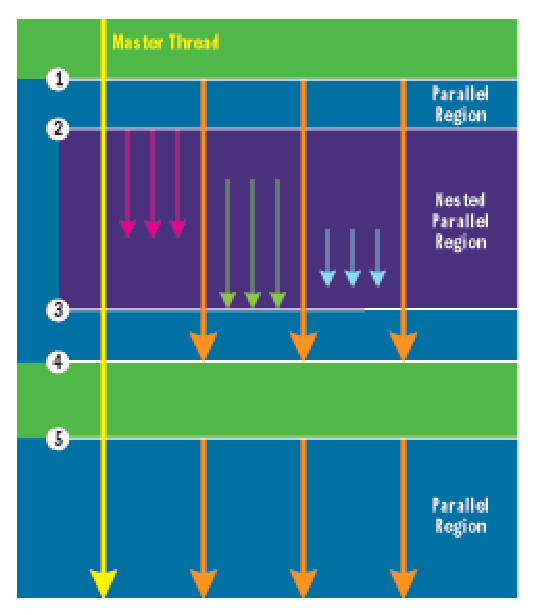
\includegraphics[height=5cm,
  angle=0]{./images/OpenMP_concept.eps}}
  \caption{OpenMP parallel sections}
  \label{fig:OpenMP_concept}
\end{figure}


\begin{figure}[hbt]
  \centerline{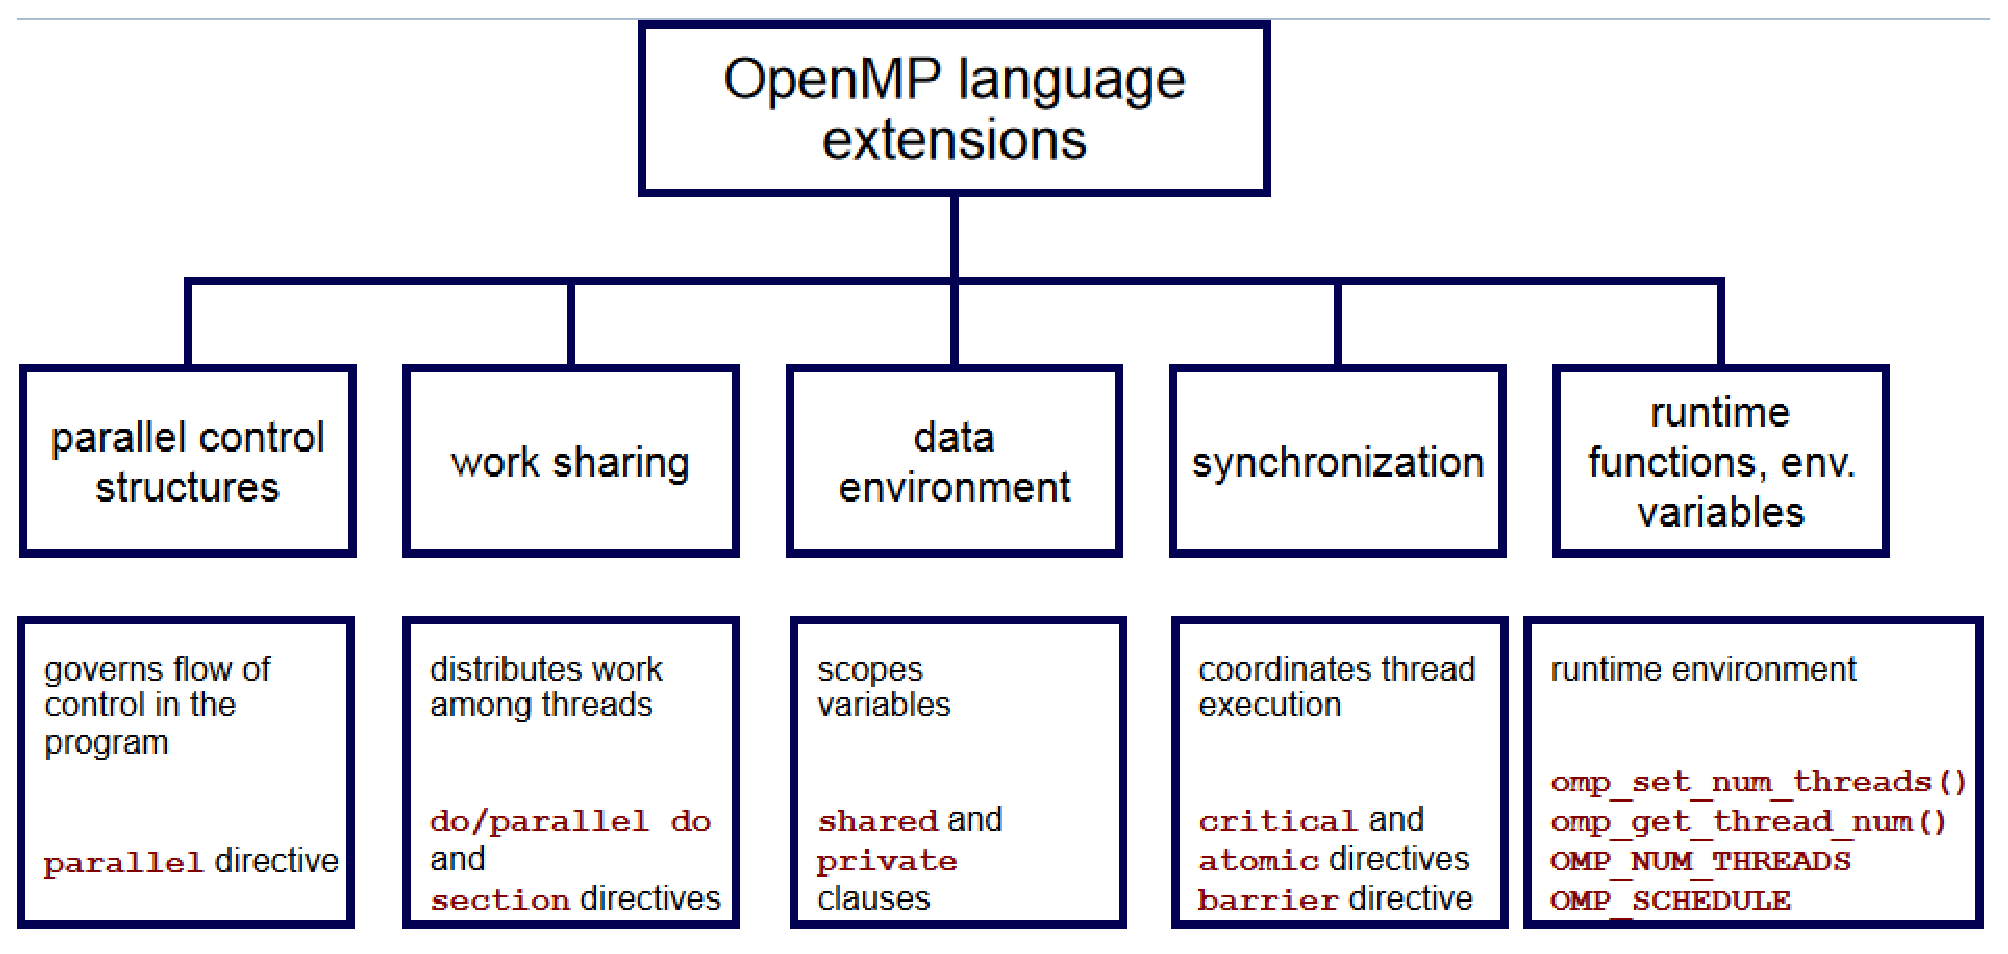
\includegraphics[height=5cm,
    angle=0]{./images/openMP_structure.eps}}
  \caption{OpenMP constructs}
\label{fig:OpenMP_core_elements}
\end{figure}

The core elements are the constructrs for thread creation, workload distribution
(work sharing), data-environment management, synchronization, and user-level
runtime functions, , Fig.\ref{fig:OpenMP_core_elements}. OpenMP consists of 2
basic constructs: pragmas and runtime routines. All OpenMP pragmas begin with
\verb!#pragma omp!.
\begin{verbatim}
#pragma omp <directive> [clause[ [,] clause]...]
\end{verbatim}

To use OpenMP, we need to include <omp.h> file
\begin{verbatim}
#include <omp.h>
\end{verbatim}
and depending the compiler, compile the code with 
\begin{itemize}
  \item \verb!-fopenmp!: GNU (gcc, g++, gfortran) with default behavior as many
  threads as available cores
  \item \verb!-openmp!: Intel (icc, ifort) with default behavior as many threads
  as available cores
  \item \verb!-mp! : Portland Group (pgf90, pgcc, pgCC, pgf77) with default
  behavior is 1 thread
\end{itemize}
To explicitly control the number of threads, see Sect.\ref{sec:set_num_threads}.

\subsection{OpenMP 2.5}

Support GNU Compiler 4.2+, MSV C++ 2005 (to enable add \verb!/openmp! to
commandline), Intel C 10.1 (use \verb!-openmp!, if enable but don't do actual
parallel execution use \verb!-openmp-stubs!).

\subsection{OpenMP 3.0}

Support GNU Compiler 4.4+, Intel C 11.0.

New features: the concept of \verb!task! and \verb!task! construct.

\subsection{OpenMP 3.1}


\subsection{OpenMP 4.0}

New features: support accelerators (heterogeneous computing), atomics
operations, error handling, thread affinity, tasking extensions, and user
defined reduction, SIMP support and Fortran 2003 support.


\section{Set number of threads}
\label{sec:set_num_threads}

The number of threads are set by the system (compilers) or can be overloaded by
environment variable or using code function. By default, the number of set is
given by the system or the compiler. Next, we can overload this using we set the
environment variable \verb!OMP_NUM_THREADS!.
\begin{verbatim}
export OMP_NUM_THREADS=4
\end{verbatim}

or at the highest level, in the code
\begin{verbatim}
#include <omp.h>

#define NUM_THREADS 4
omp_set_num_threads(NUM_THREADS);
\end{verbatim}



\section{Directives}
\label{sec:openmp_directives}

They are: parallel, for, parallel for, section, sections, single, master, critical, flush,
ordered, and atomic.

The directives can be classified into 2 forms:
\begin{enumerate}
  \item work-sharing directives: it do not create parallelism, but rather
  distribute the work into threads in the thread-team in a logical way to speed
  up the execution, i.e. the chunk of work to different threads must be
  independent.   They are:
  \verb!for!, \verb!ordered!, \verb!section!, \verb!sections!, \verb!single!.
  \item thread creation: \verb!parallel!
\end{enumerate}


\subsection{parallel ***}

This is the most important and most common directive, which create a parallel
region for the dynamic extent of the structured-block that follows
\begin{verbatim}
#pragma omp parallel [clause[ [, ]clause] ...] 
structured-block
\end{verbatim}
It tells the compiler that the code in the structured-block should be executed
in parallel on multiple threads. Each thread will execute on the 
instruction-stream, however not necessarily the same set of instructions. The
number of threads $N$ is chosen at runtime (Sect.\ref{sec:set_num_threads}).

Example:
\begin{verbatim}
#pragma omp parallel
{ 
    printf("Hello World\n");
    printf("ABC");
}
\end{verbatim}
If we don't put the block \verb!{  }!, only the next statement are put into
threads. Example:
\begin{verbatim}
#pragma omp parallel 
    printf("Hello World\n");
printf("ABC");  //only master do
\end{verbatim}

Depending on your setting, a number of threads will print out to the terminal
the two strings. As they share the  standard output, {\it race conditions}
may occur, i.e. the string are overlapped as character by character are
concurrently printed out by more than one thread.

\begin{mdframed}
Internally, GCC implements parallelism by creating amagic function and moving
the associated code into that function, and variables declared within that
blocks (or those declared outside but we ask to be private to each thread)
become local variables to the magic function (and thus, local to each thread).

Variables shared by threads are handled transparently, e.g. by passing reference
or using register variables which are flushed at the end of the parallel block
(or whenever \verb!flush! is executed).
\end{mdframed}

To be more specify in how the work should be distributed to threads, there are
additional clauses to be used
\begin{enumerate}
  \item \verb!for! or \verb!do!: $\rightarrow$ data parallelism 
  \item \verb!sections!: put consecutive (but independent) blocks of codes to
  different threads 
  \item \verb!single!: force only one thread to execute the code, a barrier is
  implied to the end
  \item \verb!master! : like \verb!single!, but ask the master thread to
  execute, and no barrier implied at the end.
\end{enumerate}

Parallelism can also be made {\it conditional}, i.e. depending on the value of
some logical expression, using  an \verb!if! clause
\begin{verbatim}
extern int some_value;

#pragma omp parallel for if (some_value)
for (int c=0; c<n; c++} {
		//do something
}

// NOTE: zero means false
\end{verbatim}

If we ignore \verb!parallel! keyword, then whatever threads available in the
current team is used to run the code in parallel. In the begining, the thread
team has only one member, the master thread. So
\begin{lstlisting}
#pragma omp for 
for (int i=0; i<n; i++){
	//do something
}
\end{lstlisting}
may be executed by only one thread, i.e. the master thread.

You can create a new thread team using 
\begin{lstlisting}
#pragma omp parallel 
{
   #pragma omp for 
   for (int i=0; i<n; i++){
      //do something
  }
	
  #pragma omp for
  for (int i=0; i<n; i++) {
      //do other things
  }

  SomeMoreCode(); //all threads execute this, but not before 
        // all threads complete the previous loop
        // NOTE: We can avoid this, i.e. allow whatever thread
        //      complete the loop to execute this code
        //      : by using 'nowait' clause in the previous #pragma
}
// always synchronize here

\end{lstlisting}
IMPORTANT: \verb!nowait! can only be used with \verb!sections!, \verb!for! and
\verb!single!. We can not use with \verb!parallel!, nor \verb!ordered! clause.

We can also specify exactly how many threads we want to create using clause
\verb!nu_threads(4)!.

\begin{verbatim}
#pragma omp parallel num_threads(4)
{


}
\end{verbatim}


More example:
\begin{verbatim}
#pragma omp parallel num_threads(2)
{
  Work1();
  #pragma omp single
  {
  	Work2();
  } //implied barrier here
  
  Work3();
}
\end{verbatim}
So, Work1() is done twice, Work2() is done once (by which thread is due to
implementation-defined, e.g. in GCC, \verb!libgomp! decides), and Work3() is
done twice. We can force the master thread to execute Work2() using
\verb!master! clause (and other threads free to execute Work3() without waiting)
\begin{verbatim}
#pragma omp master
{

} // no implicit barrier here
\end{verbatim}



\subsection{parallel + for $\rightarrow$ parallel for}
\label{sec:directive_for}

This is not what we want, as every thread does the full loop
\begin{verbatim}
#pragma omp parallel // probably not what was intended
{
for(int i = 1; i < size; ++i)
        x[i] = (y[i-1] + y[i+1])/2;
}
\end{verbatim}

What we want is that each thread does partial of the loop
\begin{verbatim}
#pragma omp parallel    
{
#pragma omp for
for(int i = 1; i < size; ++i)
        x[i] = (y[i-1] + y[i+1])/2;
}
\end{verbatim}
At the end of the parallel region, there is an {\it implicit} barrier
synchronization  that block there until the last thread completes.

Since this is the most common parallelized work-sharing construct, OpenMP
provides a short-hand 
\begin{verbatim}
#pragma omp parallel for
for(int i = 1; i < size; ++i)
    x[i] = (y[i-1] + y[i+1])/2;
\end{verbatim}

\textcolor{red}{IMPORTANT: The important of using work-sharing directives is
that we need to have a loop, and there is no dependency between iterations of
the loop.}


\verb!parallel for! or \verb!for! can be combined with some clauses:
\verb!reduction! (Sect.\ref{sec:clause_reduction})


\subsection{sections}
\label{sec:directive_sections}

\section{Data share/private}

OpenMP is the shared memory programming model, so any variable declared before
the thread creation are shared and seen by all threads. Sometimes, you want to
make them private to each thread (to avoid race conditions), we can tell the
compiler to generate new memory for these variable to each thread using data
sharing attribute clauses

\begin{enumerate}
  \item \verb!shared!
  \item \verb!private!
  \item \verb!default!
  \item \verb!firstprivate! : private and initialize to original value
  \item \verb!lastprivate!: private and original value is updated after
  construct
  \item \verb!reduction!: a safe way of joining work from all threads after the
  construct
\end{enumerate}

 By default

\section{Clauses}

\subsection{reduction}
\label{sec:clause_reduction}

\begin{verbatim}
reduction(operation:var)
\end{verbatim}


This clause can be used with some directives: \verb!for!
(Sect.\ref{sec:directive_for}), \verb!sections!
(Sect.\ref{sec:directive_sections}).


\section{Synchronization}

With multiple threads running concurrently, it's sometimes that we need to
synchronize one thread with another. One common situations is at the end of the
parallel region, before the sequential code can be executed by the master
thread, an implicit barrier synchronization is given to wait for all threads in
the thread-team to complete. 

Other places with implied barrier synchronization, at the end of each 
\verb!#pragma omp for!, \verb!#pragma omp single!, and 
\verb!#pragma omp sections! block. To remove implied barrier synchronization, we
use \verb!nowait! clause
\begin{verbatim}
#pragma omp parallel    
{
    #pragma omp for nowait
    for(int i = 1; i < size; ++i)
        x[i] = (y[i-1] + y[i+1])/2;
} // implicit barrier here

CodeWork();
\end{verbatim}

To causes all threads to wait until all other threads in the same team reach a
certain point, we put a single line with
\begin{verbatim}
#pragma omp parallel
{
   SomeCode();
   
   #pragma omp barrier
   
   // All threads need to complete SomeCode()
   // before can execute here
   SomeMoreCode();  
\end{verbatim}
to tell all threads in the thread-team to reach here before parallel execution
can be continue.

\chapter[Intel Thread Building Block]{Intel Thread Building Block (multi-core)
library}
\label{chap:TBB}

Threading Building Blocks (TBB) is a C++ template library developed by Intel for
writing software programs that take advantage of multi-core processors.

TBB is better than the following lower-level libraries
\begin{enumerate}
  \item  use of native threading packages such as POSIX threads, 
  
  \item Windows  threads, or 
  
  \item the portable Boost Threads
\end{enumerate}
as such libraries require individual threads of execution are created,
synchronized, and terminated manually.

A TBB program creates, synchronizes and destroys graphs of dependent tasks
according to algorithms, i.e. high-level parallel programming paradigms (a.k.a.
Algorithmic Skeletons - Sect.\ref{sec:Algorithmic_Skeletons}).
\textcolor{red}{Tasks are then executed respecting graph dependencies.}

\section{Introduction}

Intel TBB was under GPL license until August 2016. As of September 2016 Intel
TBB is relicensed under Apache v2.0 license.

As of September 2016 Intel TBB is dual-licensed, with a commercial (COM)
license as part of the suite products (Intel Parallel Studio, Intel System
Studio), and as open source under Apache v2.0 license.

If we run
\begin{verbatim}
make -j10
\end{verbatim}
it creates
\begin{verbatim}
./build/macos_intel64_gcc_cc4.2.1_os10.8.2_release

./build/macos_intel64_gcc_cc4.2.1_os10.8.2_debug
\end{verbatim}
in such folder, there should be tbbvars.sh and tbbvars.csh, where we can source


\url{https://github.com/01org/tbb}



\section{Algorithmic Skeletons}
\label{sec:Algorithmic_Skeletons}

Algorithmic skeletons take advantage of common programming patterns to hide the
complexity of parallel and distributed applications. Starting from a basic set
of patterns (skeletons), more complex patterns can be built by combining the
basic ones. Algorithmic skeletons were first introduced by Cole in 1989


{\it The most outstanding feature of algorithmic skeletons}, which
differentiates them from other high-level parallel programming models, is that
orchestration and synchronization of the parallel activities is implicitly
defined by the skeleton patterns. \textcolor{red}{Programmers do not have to
specify the synchronizations between the application's sequential parts.}

\url{https://en.wikipedia.org/wiki/Algorithmic_skeleton}

{\bf Non-object oriented algorithmic skeleton frameworks}

\begin{enumerate}
  \item Eden library: Haskell language
\end{enumerate}


{\bf Object oriented algorithmic skeleton frameworks}
\begin{enumerate}
  \item FastFlow library (2009-): C++ used for CUDA/OpenCL/C++11
  
   Initially developed to target multi-core platforms, and then extended to
   heterogeneous platforms composed of clusters of shared-memory platforms,
   possibly equippped with computing accelerators (CUDA, Xeon Phi, Tilera
   TILE64)
  
  FastFlow is typically comparable to (and is some cases slightly faster than)
  state-of-the-art parallel programming frameworks such as Intel TBB, OpenMP, Cilk, 
  
  {\it Skeleton set}: 
  Pipeline, Farm, ParallelFor, ParallelForReduce, MapReduce, StencilReduce,
  PoolEvolution, MacroDataFlow
  
  \item Marrow library (2013-): C++   
\end{enumerate}
\chapter[Intel Cilk]{Intel Cilk (parallel programming language)}
\label{chap:Intel_Cilk}

Like Intel TBB, Intel Cilk (Cilk++, CilkPlus) also target parallelism on
multicore processors. Intel Cilk Plus offers a competitive alternative for
parallel programming that is far easier to use than MPI.  
It is intended to complement TBB and OpenMP, enabling programmers to parallelize
applications that may be too complex or cumbersome to fit into one of these frameworks.
The tradeoff is that Cilk Plus may not be as finely tuned for specific
programming patterns or environments as TBB or OpenMP. 

\begin{mdframed}

In general, one should not expect to see performance improvements by convert an
existing parallel code in TBB or OpenMP to Cilk Plus.   TBB, OpenMP and MPI
continue to be good choices for writing High Performance Computing applications.

\end{mdframed}

Cilk is a pure programming language, started from MIT since 1990s, originally
based on ANSI C, with additional keywords target to parallelism.
Cilk became Cilk++ as the product of a new company, Cilk Arts, in 2006, and then
acquired by Intel in 2009. The final name is Intel Cilk Plus.

Intel Cilk Plus 
\begin{itemize}
  \item  eliminate the need for several of the original Cilk keywords while adding the
ability to spawn functions and to deal with variables involved in reduction operations.

  \item add array extensions, being incorporated in a commercial compiler (from
Intel), and compatibility with existing debuggers
  
\end{itemize}

The idea of Cilk: {\it the programmers expose and tell the compiler which parts
(elements) that can be safely parallelized; and the run-time environment (i.e.
the scheduler) will decide during execution how to actually divide the work
between processors}, i.e. the program runs without rewriting on different number
of co-processors (including 1).

Keywords: we need to include the header file, and use
\begin{verbatim}
_Cilk_spawn 
_Cilk_sync
cilk_spawn 
cilk_sync
\end{verbatim}
The functions that uses this must be defined with \verb!cilk! keyword.

The two main purposes of the keywords are (1) spawn a new thread, (2) sync
between the threads.

\section{\_Cilk\_spawn}

\verb!_Cilk_spawn!

\begin{verbatim}
cilk int fibonacy(int n)
{
  if (n<2) return n;
  else
  {
    int x, y;
    x = spawn fibonacy(n-1)
    y = spawn fibonacy(n-2)
    
    sync;
    return x+y;
  
  }

}
\end{verbatim}

% 
% \section{Inlet (advanced)} (no longer available in Cilk Plus)
% 
% By default, the spawn process put the returned value into the memory variable to
% the parent's frame. The alternate way is to use {\bf inlet}.
% 
% 
% An inlet is a function internal to a Cilk procedure which handles the results
% of a spawned procedure call as they return.
% A function is an inlet if it has the \verb!inlet! keyword.
% If an \verb!abort! keyword is used inside the inlet, it tells the scheduler that
% any other procedures spawned off by the parent procedure can safely be aborted.
% 
% IMPORTANT: All the inlets of a procedure are guaranteed to operate atomically
% with regards to each other and to the parent procedure, thus avoiding the bugs
% that could occur if the multiple returning procedures tried to update the same
% variables in the parent frame at the same time.
% 

\section{Hyperobjects}
\label{sec:CilkPlus_hyperobjects}


 
\part{Library}

\chapter{Algorithms}


\section{Very large computation (e.g. n!)}

Suppose factorial problem n!, when using \verb!long long! data type, it exceeds
the size at 20!
\begin{verbatim}

121645100408832000      <-  18!
2432902008176640000     <-  19!
-4249290049419214848    <-  20!
\end{verbatim}


This is based on the idea of carried over of multiplication
\begin{verbatim}
   12
 x 13
 -------
   36  = 3x12
  12   = 1x12
 --------
  158   
\end{verbatim}

Solution, either use a string of character, or an array in which each element
keep a single digit. NOTICE that as we now the less-significant number first, so
they will be stored as the first element in the array. So '123' is stored as 
a = [3,2,1]. This is important for I/O purpose that we need to go through from
a[m-1] to a[0].

\begin{verbatim}
int a[200]; //array will have the capacity to store 200 digits.
            // we actually can use 'byte' to save memory

int m;  //keep the maximum index being used, i.e. a[0] ... a[m-1]
int temp; //keep the carry value
\end{verbatim}

\begin{verbatim}
a[0] = 1;
m = 1;
temp = 0;

for (int i = 0; i <= n; i++)
{
  for (int j = 0;j < m; j++)
  {
     int x = a[j] * i + temp; //digit-by-number product
     a[j] = x%10; //contain the less-significant digit
     temp = x/10; //contain the carry value
  }
  while (temp > 0)
  {
     a[m] = temp%10;
     temp = temp/10;
     m++;
  }
} 
\end{verbatim}

Now to print,
\begin{verbatim}
for (int i = m-1;0; i--)
  print(%d, a[i]);
  
\end{verbatim}
\section{Recursion}

A function that call itself is called a recursive function
\begin{verbatim}
def recsum(x):
 if x == 1:
  return x
 else:
  return x + recsum(x - 1)
\end{verbatim}
The function doesn't returns, as it need to call a function and that function
need to be completed before a sum with 'x' can be done and return the value.

Each functional call creates a stack frame in the call stack
(Sect.\ref{sec:heap_stack}). The problem with this is that if the number of
recursive call is too large, \textcolor{red}{stack overflow} error may occur.

A solution is to use {\it tail-recursive} function. The recursive call is the
last thing that happens so the functional call can be replaced with a jump to
the function's entry point. \textcolor{red}{Most current gcc compilers do
tail-call optimization.} Here, the result is passed as an argument to the
function, so that the result is constantly updated as each function call
\begin{verbatim}
def tailrecsum(x, running_total=0):
  if x == 0:
    return running_total
  else:
    return tailrecsum(x - 1, running_total + x)
\end{verbatim}
The function returns, and call another function. So, we don't have the problem
of stack overflow.

In C++: the n! = 1.2.3\ldots. n
\begin{verbatim}
int factorial(int n, int acc=1) {
  if (n <= 1) return acc;
  else        return factorial(n-1, n*acc);
}
\end{verbatim}
However, this actually calculate n.(n-1).(n-2)\ldots1. It means that it requires
the operator, i.e. multiplication, is both associative and commutative. This is
luckily correct, in this case, but again, not true for a general operator. A
better solution is
\begin{verbatim}
int factorial(int n, int k = 1, int acc=1) {
  if (n <= 1) return acc;
  else        return factorial(n-1, k+1, k*acc);
}
\end{verbatim}
\url{http://stackoverflow.com/questions/15537432/convert-recursion-to-tail-recursion}

What if the problem is double-recursion, like the Fibonacci problem
\begin{verbatim}
F(n) = F(n-1) + F(n-2)
\end{verbatim}
with
\begin{verbatim}
F1 = 1, F2 = 1
or 
F1 = 0, F2 = 1
\end{verbatim}

Using \verb!f_a! as F(n-1) and \verb!f_b! as F(n-2)
\begin{verbatim}
int fibonacci(int n, int f_a =1, int f_b = 1)
  if (n == 0) return f_a;
  else   return fibonacci(n-1, f_a+f_b, f_a)
}
\end{verbatim}

CONCLUSION: By keep adding enough parameters to the tail-recursive function, it
can solve for a recursive sequence where each element can be expressed by some
formula of the previous $k$ elements.

\section{std::transform}
\label{sec:std::transform}

We can apply unitary operation or binary operation.
However, std::transform does not guarantee in-order application.
To apply a function to a sequence in-order or to apply a function that modifies
the elements of a sequence, use \verb!std::for_each!
(Sect.\ref{sec:std::for_each})

{\bf unitary operation}
\begin{verbatim}
#include <algorithm>

//assume 's' is some iterable object (e.g. array, vector)
std::transform( s.begin(), s.end(), unitary_operator)

// with unitary_operator can be
// 1. lambda
 std::string s("hello");
    std::transform(s.begin(), s.end(), s.begin(),
                   [](unsigned char c) { return std::toupper(c); });
    std::cout << s;
\end{verbatim}
Sect.\ref{sec:}

{\bf binary operator}
\begin{lstlisting}
//assume 'si' is some iterable object (e.g. array, vector)
std::transform( s.begin(), s.end(), s2.begin(), result.begin(), binary_operator)
\end{lstlisting}
\url{http://stackoverflow.com/questions/13728430/element-wise-multiplication-of-two-vectors-in-c}

\section{std::for\_each}
\label{sec:std::for_each}

\section{Reduction}

\subsection{Sum}

\begin{verbatim}
vector<int> V{1,2,3};  

sum = 0;  // 0 - value of 3rd param
for (auto x : V)  sum += x;
\end{verbatim}

Another way is using 
\begin{enumerate}
  \item std::accumulate
\end{enumerate}

\subsection{-- std::accumulate}
\label{sec:std::accumulate}

This is a reduction operation
\begin{verbatim}
vector<int> V{1,2,3};  
// NOTE: 0 is the initial value for the reduction operation
// sum = 0 + V[0] + V[1] + ...
int sum = accumulate(V.begin(), V.end(), 0);
// sum == 6
\end{verbatim}
It is important to choose the right matrix.

There is also optional 4th parameter, which allow to replace addition with any
other operation.

\begin{verbatim}
vector<int> V{1,2,3};
int product = accumulate(V.begin(), V.end(), 1, multiplies<int>());
\end{verbatim}

\url{http://stackoverflow.com/questions/12633950/understanding-stdaccumulate}
\chapter{Boost library}
\label{chap:Boost-library}
\label{sec:Boost-library}

There are three kinds of libraries:
\begin{enumerate}
  \item Header-only libraries: dependencies are resolved at compile time
  \item Static libraries: dependencies are resolved at link time
  \item Dynamic (shared) libraries: dependencies are resolved at run-time
\end{enumerate}

Boost is not a single library, but a collection of many libraries (58
libraries in Boost 1.32.0), written by different authors. Many of Boost
components are header-only libraries. 

The Boost organization has a standard for adding a new library into Boost. Boost
makes C++ programming more elegant, robust and productive.

Many libraries in Boost are now a part of the Standard Template Library (STL) in
the new C++ specification, C++11. So, it's suggested to use C++11 features if
possible. 

NOTE: Any thing from the STL, it starts with \verb!std::!; while those from
Boost, it starts with \verb!boost::!. 

Comparison of features in C++11 STL vs. Boost
\footnote{\url{http://stackoverflow.com/questions/8851670/relevant-boost-features-vs-c11}}
\begin{enumerate}
  \item Boost.Lambda = lambda expression (in non-polymorphic case) 
  
  NOTE: Boost.Lambda is still useful for polymorphic lambdas
  
  \item Chrono (Sect.\ref{sec:Boost.Chrono}) = now part of C++11 \verb!#include!
  \verb!<chrono>! - Sect.\ref{sec:chrono-header-file}
   
    
  \item Foreach (\verb!BOOST_FOREACH!) = range-based for
  
  \item Functional/Forward = perfect forwarding (rvalue references, variadic
  templates, std::forward)
  
  NOTE: Boost Functional/Hash
  \footnote{\url{http://www.boost.org/doc/libs/1_53_0/doc/html/hash.html}}
  contains some functions not found in C++11, e.g. \verb!hash_combine!
  
  NOTE: A large part of Boost MPL library
  \footnote{\url{http://www.boost.org/doc/libs/1_53_0/libs/mpl/doc/index.html}}
  can be replaced by using variadic templates
  
  \item Local function = Lambda expression

  \item Some common use cases of Boost Lexical-cast
  \footnote{\url{http://www.boost.org/doc/libs/1_53_0/doc/html/boost_lexical_cast.html}}
  can be replaced by \verb!std::to_string! and \verb!std::stoX!.
  
  \item Min-Max = std::minmax, \verb!std::minmax_element!
  \item Move = rvalue reference
  \item Ratio = \verb!std::ratio!
  \item static assert = \verb!static_assert!
  \item Thread = \verb!#include <thread>!
  \item Typeof = 'auto', 'decltype' keywords
  \item Value initialization = List-initialization
  \item Array = \verb!std::array!
  \item Bind = \verb!std::bind!
  \item Enable If = \verb!std::enable_if!
  \item Function = \verb!std::function!
  \item Member function = \verb!std::mem_fn!
  \item Random = \verb!#include <random>!
  \item Ref  = \verb!std::ref!, \verb!std::cref!
  \item Regex = regular expression \verb!#include <regex>!
  
  NOTE: C++11 doesn't support Perl5 regular expression like Boost Regex. Certain
  \verb!regex! interface members (e.g. \verb!boost::basic_regex<>::empty()!) is
  exactly matched with Boost Xpressive; and play much more nicely with Boost
  String Algorithms, which doesn't a C++11 standard counterparts yet.
  
  \item Utility, e.g. \verb!boost::result_of<>! =  \verb!std::result_of!
  
  \item Smart Pointer = \verb!std::unique_ptr!, \verb!std::shared_ptr!,
  \verb!std::weak_ptr! (KEEP \verb!boost::intrusive_ptr!)
  
  NOTE: \verb!std::unique_ptr! is part of TR1 (Sect.\ref{sec:unique_ptr}).
  
  \verb!const std::unique_ptr! replaces the use of \verb!boost::scoped_ptr! and
  \verb!boost::scoped_array!
  
  \item Swap (swapping arrays) = now part of C++11 \verb!std::swap!
  
  \item Tuple = now part of C++11 \verb!std::tuple! - Sect.\ref{sec:std::tuple}
  
  \item Type Traits = now part of C++11 \verb!#include <type_traits>! -
  Sect.\ref{sec:type_traits-header}
  
  NOTE: C++11 doesn't support \verb!call_traits! like Boost Type Traits.
  
  \item Unordered = \verb!#include <unordered_set>!, \verb!#include!
  \verb!<unordered_map>!
   
  \item Range = \verb!std::tie!, \verb!std::begin!
\end{enumerate}


\section{Overview}

\subsection{What is Boost.Build (b2)?}
\label{sec:Boost.Build}
\label{sec:b2-program}

Boost.Build is a high-level build system which makes it as easy as possible to
manage C++ projects.
The idea is to use configuration files just as much as necessary to build a
program.
Boost.Build supports many compilers out of the box and knows how to use them.
\url{https://boostorg.github.io/build/}

\url{https://www.boost.org/doc/libs/1_64_0/tools/build/tutorial.html}

Boost.Build translates options in configuration files to command line options
expected by the selected compiler.

However, regardless as nice as it sounds, Boost.Build can only be used for C++ and C projects.
Boost.Build doesn't know how to use other compilers like a Java compiler. 


ORIGINAL APPLICATATION:
Boost.Build was created to build and install the Boost C++ libraries easily with
different compilers on different platforms.

\url{https://www.boost.org/doc/libs/1_63_0/tools/build/tutorial.html}

Boost.Build uses a programm called {\bf b2} (previously it is called {\bf
bjam}). b2 looks for configuration files, reads them and builds a project
accordingly. b2 does indeed look for two more configuration files when it
starts.
\begin{enumerate}
  
  \item site-config.jam: used to set options for an entire system. This file is
  controlled by sys-admin, and not everyone can modify it.
  
In Boost, the file name is \verb!project-config.jam! file [which is generated by ./bootstrap.sh script]
\begin{verbatim}
./bootstrap --prefix=/path/to/install
\end{verbatim}

  \item \verb!user-config.jam!: b2 also looks for a file user-config.jam in a user's home director
  
As the file user-config.jam can be maintained by users it is probably used more
often than site-config.jam.
 
As these configuration files do not belong to a project but to a machine or a
user on a machine they are allowed to contain machine-specific options.

\end{enumerate}


\begin{mdframed}


The Boost.Build engine is derived from an earlier build tool called Perforce
Jam.
Originally, there were just minor changes, and the filename was bjam.
With more changes, as of Boost 1.47.0, the official name of the executable was
changed to b2. A copy named bjam is still created for compatibility, but you are
encouraged to use the new name in all cases.

\end{mdframed}


The configuration file b2 is looking for is a file with extension \verb!*.jam!,
called Jamfile.jam.


When the build system is loaded it also prepares itself to use a certain
compiler, linker and maybe other tools required to build a project. Boost.Build
refers to these programs as a {\bf toolset}. As of today there are more than 10 toolsets supported.

If no command line option is used to start b2 the build system tries to find a
toolset it can use automatically. To manually select a toolset, run ./b2 with option
toolset=something.

\begin{verbatim}
#If you want GCC to be used 
./b2 toolset=gcc


warning: No toolsets are configured.
warning: Configuring default toolset "msvc".
warning: If the default is wrong, your build may not work correctly.
warning: Use the "toolset=xxxxx" option to override our guess.
warning: For more configuration options, please consult
warning: http://boost.org/boost-build2/doc/html/bbv2/advanced/configuration.html
\end{verbatim}

\subsection{example *.jam file: simplest}

The programming language Boost.Build is based on knows only one data type:
Everything is a list of strings. A list can be empty or contain one or more
strings.


It means create an 'exe' file, name 'hello', using source file 'hello.cpp'
\begin{verbatim}
exe hello : hello.cpp ; 
\end{verbatim}
Boost.Build will detect the proper toolset, e.g. GCC in this case.

Boost.Build provides a lot of built-in rules and {\bf exe} is one of them, which
is a function. The function exe is called with two parameters each one a list
containing one string. In the Jamfile above the function exe is called with the
two parameters hello and hello.cpp.

It is possible to use quotes
\begin{verbatim}
exe "hello" : "hello.cpp" ; 
\end{verbatim}
There is no special character to separate a rule name and the first parameter, i.e. just a space is enough.
Then, a colon must be used to separate other parameters; and a space must be followed. 

IMPORTANT: Without spaces around tokens b2 won't be able to parse Jamfiles correctly.

Another important rule is lib. It is used to build a library.
\begin{verbatim}
lib world : world.cpp ; 
\end{verbatim}
By default, a shared library is built.
\begin{verbatim}
lib world : world.cpp : <link>static ; 
\end{verbatim}


\subsection{example *.jam file: <variant> option}

The fourth parameter contains features which are used by default but which can be overwritten.
\begin{verbatim}
exe hello : hello.cpp : <variant>release ; 

exe hello : hello.cpp : : <variant>debug <variant>release ; 
\end{verbatim}
As a program can't be a debug and a release version at the same time <variant> must be set in the default values, 
the <variant> feature needs to be set twice to debug and release.

Only then Boost.Build understands that two versions of hello.exe should be built.

\subsection{: <define> option}
\begin{verbatim}
exe hello : hello.cpp : <define>WIN32 <define>_WIN32 : <variant>debug <variant>release ; 

\end{verbatim}

The feature <define> is used to define preprocessor directives

A debug version optimized for speed, a debug version with no optimization, a release version optimized for speed and a release version with no optimization.
All of these versions are built in seperate directories which are automatically created.
\begin{verbatim}

exe hello : hello.cpp : : <variant>debug <variant>release <optimization>speed <optimization>off ; 

\end{verbatim}


A variant is a debug or release version of a program. For each variant another
directory is used to build a program - again for the reason not to overwrite
files produced by another variant.

By default the debug variant is used. If you want a release version to be
created you can specify the variant on the command line with b2 variant=release
or, even simpler, b2 release .

There are not only toolset-specific directories but also variant-specific
directories.


If you don't want to specify the variant on the command line but want to build
release versions of hello.exe by default the Jamfile has to be changed.
\begin{verbatim}
exe hello : hello.cpp : <variant>release ; 
\end{verbatim}

\subsection{How to install}

There is a script \verb!./bootstrap.sh! which accepts a number of command-line options to help creating 
\begin{verbatim}
JAM_CONFIG_OUT=project-config.jam
\end{verbatim}
file. 

\begin{verbatim}
./bootstrap.sh --prefix=/usr/local/boost-1.68.0

./bootstrap.sh --prefix=/packages/boost/1.68.0 --with-python-version=3.6

\end{verbatim}

or check python location, e.g. /packages/anaconda3/3.4.1/bin
\begin{verbatim}
./bootstrap.sh  --prefix=/packages/boost/1.68.0 \
     --with-python=/packages/anaconda3/3.4.1/bin/python3
     --with-python-version=3.6
     --with-python-root=/packages/anaconda3/3.4.1/

\end{verbatim}
or just run with 
\begin{verbatim}
./bootstrap.sh  --prefix=/packages/boost/1.68.0 --with-python-version=X.Y
\end{verbatim}


Then, we can modify this file accordingly. In earlier version of Boost, they
mentions the file \verb!user-config.jam!.
NOTE: We can either rename to the oldname by editing \verb!bootstrap.sh!
\begin{verbatim}
//change this
cat > project-config.jam <<EOF

//to
cat > user-config.jam <<EOF
\end{verbatim} 
or to use your own file we pass
\begin{verbatim}
./bjam --user-config=user-config.jam
\end{verbatim}

NOTE: We should use \verb!project-config.jam!, rather than
\verb!user-config.jam!.


Finally, to build, we run
\begin{verbatim}
sudo ./b2 -d+2  install
\end{verbatim}

 \url{https://lists.boost.org/Archives/boost/2017/10/239485.php}
\begin{verbatim}
On a not entirely unrelated note, Rene Rivera has added a new feature 
<cxxstd> to Boost.Build that controls the C++ standard in use. So for 
instance, instead of the old 
    b2 libs/mylib/test toolset=gcc cxxflags=-std=c++11 
one can now use 
    b2 libs/mylib/test toolset=gcc cxxstd=11 
In addition to being more convenient, this also allows several invocations 
to be combined into one: 
    b2 libs/mylib/test toolset=clang cxxstd=03,11,14,1z 
\end{verbatim}
\url{https://gist.github.com/dennycd/5890475}

\subsection{-- explains}

As \verb!b2! (Boost.Build) is used, it loads the first jam file
\verb!boost-build.jam!, regardless from which Boost library subfolder. It allows us to choose 
which Boost.Build installation to use, unless overriden via command-line options, and
\begin{verbatim}
BOOST_BUILD ?= tools/build/src
\end{verbatim}
The file 
\begin{verbatim}
$BOOST_BUILD/build-system.jam
\end{verbatim}
tells the default toolset, based on the O/S.

In Mac O/S, Clang is the default; while in Linux, GCC is the default. 


IMPORTANT: a C++ library compiled with GCC is not compatible with Clang and
vice-versa. So, you won’t be able to use a Clang build Boost with GCC.
 
\subsection{-- project-config.jam file}

If you use the default setting, the build is straightforward, run boostrap.sh to generate 
project-config.jam file 
\begin{verbatim}

# default (install all Boost libraries)
./bootstrap.sh --prefix=/usr/local/boost-1.68.0

# (select some libraries)
./bootstrap.sh --prefix=/usr/local/boost/1_68_0 --with-libraries=chrono,system,thread,timer,signals,random,date_time,coroutine

#  it's probably better to use the dedicated cxxstd feature. 
# You could add it to project-config.jam as <cxxstd>14, or pass it when building, as in b2 cxxstd=14.

# compile with C++14 standard --> some functions in Boost libraries are only available with C++14
sudo ./b2 cxxstd=14 install

\end{verbatim}

If you want to use a different GCC version, first be sure that you have GCC 8
installed and available in your path.

\begin{verbatim}

#edit project-config.jam [see below]

sudo ./b2 cxxflags=-std=c++17 install
\end{verbatim}

Edit file: Feel free to change 8.1 to match the version of GCC you have 

\begin{verbatim}
#if ! darwin in [ feature.values <toolset> ]
#{
#    using darwin ;
#}

#project : default-build <toolset>darwin ;
 
#using gcc : 8.1 : /usr/local/gcc-8.1/bin/g++-8.1 : <cxxstd>14 ; # C++ 14

using gcc : 7.3 : /packages/gcc/7.3/bin/gcc : <cxxflags>-std=c++14 <link>=shared ; # C++ 14

#using gcc : 8.1 : /usr/local/gcc-8.1/bin/g++-8.1 : <cxxflags>-std=c++14 ; # C++ 14

import python ;
#if ! [ python.configured ]
#{
#    using python : 3.6 : /packages/anaconda3/5.2.0 ;
#}
using python
    : 3.6                   # Version
    : /packages/anaconda3/5.2.0/bin/python # Python path
    : /packages/anaconda3/5.2.0/include/python3.6m/  # include path
    : /packages/anaconda3/5.2.0/lib  # lib paths
;

\end{verbatim}
\url{https://github.com/boostorg/system/issues/26}

\url{https://boostorg.github.io/build/manual/develop/index.html}

NOTE: We can define as many variants/toolset as we like, with the tilde to delineate a variation
\begin{verbatim}
using gcc : 5 : g++-5 : ; # default is C++ 98
using gcc : 5~c++03 : g++-5 : <cxxflags>-std=c++03 ; # C++ 03
using gcc : 5~gnu03 : g++-5 : <cxxflags>-std=gnu++03 ; # C++ 03 with GNU
using gcc : 5~c++11 : g++-5 : <cxxflags>-std=c++11 ; # C++ 11
using gcc : 5~c++14 : g++-5 : <cxxflags>-std=c++14 ; # C++ 14
\end{verbatim}

and when we run with \verb!./b2! we can select 
\begin{verbatim}
# toolset name first (gcc) and then dash (-) before the version+variation (5~c++14)
b2 toolset=gcc-5 stage
b2 toolset=gcc-5~c++14 stage
\end{verbatim}

ISSUE with Anaconda Python in project-config.jam
\begin{verbatim}
using python : 3.6 : /home/myUser/anaconda3 ; 

\end{verbatim}
If we build
\begin{verbatim}
sudo ./b2 --with-python -j8 install
\end{verbatim}
then an error
\begin{verbatim}
./boost/python/detail/wrap_python.hpp:50:11: fatal error: 
pyconfig.h: No such file or directory
# include <pyconfig.h>
          ^~~~~~~~~~~~
compilation terminated.
\end{verbatim}
SOLUTION: we need to use
\begin{verbatim}
C_INCLUDE_PATH /packages/anaconda3/5.2.0/include/python3.6m/
CPLUS_INCLUDE_PATH /packages/anaconda3/5.2.0/include/python3.6m/
\end{verbatim}
\url{https://stackoverflow.com/questions/54152667/how-to-fix-pyconfig-h-not-found-with-anaconda}

EDIT THE FILE: Btw, to enable MPI support, we add to the file project-config.jam
\begin{verbatim}
using mpi ; #to enable MPI support

#or tell it where to look for the file as well
# check <boost>/build/v2/tools/mpi.jam

using mpi : /usr/local/mpich2-1.0.4/bin/mpiCC;
\end{verbatim}
\url{https://www.boost.org/doc/libs/1_61_0/doc/html/mpi/getting_started.html}


EDIT THE FILE: TO compile with python 3
\begin{verbatim}
   using python : 3.5 :  /path/to/python/root : /path/to/python/include : /path/to/python/libs ;
\end{verbatim}
[NOTE: In Windows, use \verb!\\! for path]

Example:
\begin{verbatim}
  // early name when it is a folk of JAM build system
./bjam install --prefix=PREFIX

 // now is b2 as it is very much different from the original 'JAM'
./b2 install --prefix=PREFIX


./b2 toolset=clang cxxflags="-stdlib=libc++ -std=c++11" linkflags="-stdlib=libc++ -std=c++11" 

./b2 toolset=gcc cxxflags=-std=c++14 --prefix=/packages/boost/1.6.80s --with-mpi
\end{verbatim}

Here we use PREFIX=\verb!/usr/local/boost!. Other useful options
\begin{verbatim} 
  //to provide more details
--debug-configuration 
  //to force enable MPI
--with-mpi
  //suppress the warning message when no MPI is supported
--without-mpi

  // to build only Boost.Python
--with-python
\end{verbatim}


HOW TO USE: here we link to two different libraries inside boost (e.g. boost:system and boost::filesystem)
\begin{verbatim}
g++-8.1 -std=c++17 -I /usr/local/boost-1.68.0/include -L /usr/local/boost-1.68.0/lib test.cpp -o test -lboost_system -lboost_filesystem

clang++ -std=c++17 -I /usr/local/boost-1.68.0/include -L /usr/local/boost-1.68.0/lib test.cpp -o test -lboost_system -lboost_filesystem

\end{verbatim}

\url{https://solarianprogrammer.com/2018/08/07/compiling-boost-gcc-clang-macos/}

You may want to install first
\begin{enumerate}
  \item bzip2 header files: 
  \begin{verbatim}
  #RED-HAT
  sudo yum install bzip2-devel.x86_64
  
  #UBUNTU
  \end{verbatim}
  NOTE: To search for package names, if you don't remember exactly the name in
  RedHat
  \begin{verbatim}
  sudo yum search bzip
  \end{verbatim}
  
  \item python header files:
  \begin{verbatim}
  sudo yum install python-devel.x86_64
  \end{verbatim}
  
  \item You may also want to modify the \verb!user-config.jam! file
  
  Copy the template from
  \begin{verbatim}
  boost_<version>/tools/build/v2/user-config.jam

OR
  boost/tools/build/user-config.jam

  \end{verbatim}
  into boost source directory
  
\end{enumerate}

The default installation folder is /usr/local/
\begin{verbatim}
Boost_DIR=/usr/local/boost_1_53_0
Boost_INCLUDE_DIR=/usr/local/boost_1_53_0/include/

Boost_LIB_DIR=/usr/local/boost_1_53_0/lib
\end{verbatim}
For many of the libraries in Boost, we only need the header files. However, some
requires the compiled shared libraries as well.

\subsection{Link your code agains boost}


If your code use Boost MPI, then you need to link against \verb!boost_mpi! and
\verb!boost_serialization!
\begin{verbatim}
mpic++ your_code.cpp   \
   -Llibdir -lboost_mpi-gcc-mt-1_35 -lboost_resialization-gcc-d-1_35.a
\end{verbatim}
If you also want to use Python-bindings for Boost.MPI, then
\begin{verbatim}
... 
-lboost_mpi_python-gcc-mt-1_35
\end{verbatim}
to your link command. This is necessary only if you register C++ types and use
skeleton/content mechanism (i.e. how to transfer large data structures
created in C++ to be used in Python code) from Python.

\section{a new way of using Boost with CMake}


Now for every Boost library there is a *.cmake file) instead of the one from CMake distribution


\section{boost::spirit (format data, parse data)}
\label{sec:boost_spirit}


Spirit was added to Boost since Boost 1.30.0 (March, 19th, 2003). The code base
of Spirit 1.8.x becomes \verb!Spirit.Classic! component in Spirit 2.x. 
\begin{itemize}
  \item Spirit 2.0 was added to Boost 1.37.0
  \item Spirit 2.1 was added to Boost 1.41.0:
  \item \ldots 
  \item Spirit 2.5 was added to Boost 1.47.0
  \item Spirit 2.5.1 was added to Boost 1.48.0
\end{itemize}

Spirit 2.5.1 has 4
components:\footnote{\url{http://boost-spirit.com/home/wp-content/uploads/2010/05/spirit_presentation.pdf}}
\begin{enumerate}
  \item boost::spirit::qi    (parsing input)
  \item boost::spirit::karma (generating output)
  \item boost::spirit::lex   (a lexer)
  \item boost::spirit::classic (old-parsing input). Any
existing code either uses the old Spirit (example:
Sect.\ref{sec:boost_spirit_classic}), or need to update the header files in
\begin{verbatim}
$BOOST_ROOT/boost/spirit/include
\end{verbatim} 
with \verb!classic_! prefix in the
names. E.g. 
\begin{verbatim}
#include <boost/spirit/include/core.hpp>
\end{verbatim}
becomes 
\begin{verbatim}
#include <boost/spirit/include/classic_core.hpp>
\end{verbatim}
and use the new namespace \verb!boost::spirit::classic!.

\end{enumerate}

\subsection{Lexer vs. Parser}

{\bf A lexer vs. A parser}: a lexer converts a sequence of characters into a
sequence of {\it tokens}. A lexer often exist as a single function which is
called by the parser. A token is a string of one or more characters that can be
classified into {\it token-type}. E.g.: 'sum'=identifier, '=' is assigment
operator, '3' or '2'=integer literal, ';' = end of statement. To define a token,
we can use {\it regular expressions}.

To interpret the data (in any form), and convert it into another form
using, the tool is called a {\it parser}. The parser can check if the input has
a correct format (in the case of file I/O), or a correct syntax (in the case of a
scripting language or programming language).


\subsection{Grammar presentation}

By defining a proper grammar specification, it can tell whether input follow the
grammar or not. What we want to parse can be anything (from email, command
lines, scritting languages, etc.). Languages are often ambiguous by nature. To
avoid this ambiguity (as much as we can), programming language are often
designed as {\bf context-free grammar} (CFG).

The rules are called Extended Backus-Nauer Form (EBNF) production rules. The
grammar describes both input and output. There are different ways to define a
grammar specification. The two major families of approaches are bottom-up
parsing and top-down parsing. It's expected that the language to be parsed is
{\bf context-free grammar}, i.e. the production rule is in the form
$V\rightarrow w$ ($w$ can be empty or a string of terminals or non-terminals,
$V$ is single non-terminal symbol).
\begin{enumerate}
  \item Top-down parsing: LL parser (or LL(k) parser if it use $k$ tokens of
  lookahead when parsing the input: parse from Left to Right, and construct
  Leftmost derivation
  tree)\footnote{\url{http://en.wikipedia.org/wiki/LL_parser}}. 
  
  Recursive descent parser is a kind of top-down parser that works only for
  LL($k$) grammars, built from a set of mutually recursive procedures (or
  non-recursive equivalent), each procedure implement one of the production rule
  of the grammar. It's pretty to implement using functional languages (Haskell,
  Lisp, etc.). \textcolor{red}{C and C++ parser of GCC uses this approach}.
  
  Tools to generate LL parsers are ANTLR (which can generate parser in C,
  C\#, Java, JavaScript, Objective-C, Perl, Ada95,
  etc.\footnote{\url{http://en.wikipedia.org/wiki/ANTLR}}),
  \verb!boost::spirit!.

  \item Bottom-up parsing: LR parser
  (Donald Knuth invented LR parser (Left-to-Right, Rightmost derivation) in
  1965). Variants of LR parser are LALR parser (Look-Ahead LR parser: done by
  shift-reduce parser), SLR parser (Simple LR parser), both proposed by Frank
  DeRemer in 1969 to avoid using large memory.
  
  Tools to generate LALR parsers are YACC, Bison
\end{enumerate}
NOTE: Understanding righe-derivation is harder than left-derivation. 

\verb!boost::spirit! is a recursive descent parser; with
\verb!boost::spirit::qi! is a fully object-oriented LL(k) parser and
lexical analyzer. Spirit treats both processes virtually identical. In
\verb!boost::spirit::qi!, a {\bf parser} is a small object that know how to
parse a particular string.  Traditionally, \verb!lex/flex!/ \verb!yacc/bison!
are widely used tools. The grammar can be built using primitive parsers, and
can be combined using overloadeed C++ operators. 

A grammar always start with the first parser, whose associated attribute is the
{\bf abstract syntax tree} (AST), which is a tree representation of the
syntactic structure of the source code.

An example of LL(1) from, terminals are expressed in quotes
{\small \begin{verbatim}
 program = block "." .
 
 block =
     ["const" ident "=" number {"," ident "=" number} ";"]
     ["var" ident {"," ident} ";"]
     {"procedure" ident ";" block ";"} statement .
 
 statement =
     ident ":=" expression
     | "call" ident
     | "begin" statement ";" {statement ";"} "end"
     | "if" condition "then" statement
     | "while" condition "do" statement .
 
 condition =
     "odd" expression
     | expression ("="|"#"|"<"|"<="|">"|">=") expression .
 
 expression = ["+"|"-"] term {("+"|"-") term} .
 
 term = factor {("*"|"/") factor} .
 
 factor =
     ident
     | number
     | "(" expression ")" .
\end{verbatim}}

A C implementation of a parser for the above grammar using recursive descent
parser approach
\lstset{language=C,
numberstyle=\footnotesize,
basicstyle=\ttfamily\footnotesize,
frame=shadowbox,
breaklines=true
}
\begin{lstlisting}
typedef enum {ident, number, lparen, rparen, times, slash, plus,
    minus, eql, neq, lss, leq, gtr, geq, callsym, beginsym, semicolon,
    endsym, ifsym, whilesym, becomes, thensym, dosym, constsym, comma,
    varsym, procsym, period, oddsym} Symbol;
 
Symbol sym;
void getsym(void);
void error(const char msg[]);
void expression(void);
 
int accept(Symbol s) {
    if (sym == s) {
        getsym();
        return 1;
    }
    return 0;
}
 
int expect(Symbol s) {
    if (accept(s))
        return 1;
    error("expect: unexpected symbol");
    return 0;
}
 
void factor(void) {
    if (accept(ident)) {
        ;
    } else if (accept(number)) {
        ;
    } else if (accept(lparen)) {
        expression();
        expect(rparen);
    } else {
        error("factor: syntax error");
        getsym();
    }
}
 
void term(void) {
    factor();
    while (sym == times || sym == slash) {
        getsym();
        factor();
    }
}
 
void expression(void) {
    if (sym == plus || sym == minus)
        getsym();
    term();
    while (sym == plus || sym == minus) {
        getsym();
        term();
    }
}
 
void condition(void) {
    if (accept(oddsym)) {
        expression();
    } else {
        expression();
        if (sym == eql || sym == neq || sym == lss || sym == leq || sym == gtr || sym == geq) {
            getsym();
            expression();
        } else {
            error("condition: invalid operator");
            getsym();
        }
    }
}
 
void statement(void) {
    if (accept(ident)) {
        expect(becomes);
        expression();
    } else if (accept(callsym)) {
        expect(ident);
    } else if (accept(beginsym)) {
        do {
            statement();
        } while (accept(semicolon));
        expect(endsym);
    } else if (accept(ifsym)) {
        condition();
        expect(thensym);
        statement();
    } else if (accept(whilesym)) {
        condition();
        expect(dosym);
        statement();
    } else {
        error("statement: syntax error");
        getsym();
    }
}
 
void block(void) {
    if (accept(constsym)) {
        do {
            expect(ident);
            expect(eql);
            expect(number);
        } while (accept(comma));
        expect(semicolon);
    }
    if (accept(varsym)) {
        do {
            expect(ident);
        } while (accept(comma));
        expect(semicolon);
    }
    while (accept(procsym)) {
        expect(ident);
        expect(semicolon);
        block();
        expect(semicolon);
    }
    statement();
}
 
void program(void) {
    getsym();
    block();
    expect(period);
}
\end{lstlisting}  

\subsection{Change Logs}

\begin{enumerate}
  \item  Spirit::Qi V2.1 code changes: (1)
  \verb!qi::phrase_parse!, \verb!qi::phrase_format! do post-skip by default, (2)
  attributes is always the last parameter in the functions
  \begin{verbatim}
  qi::phrase_parse()
  qi::phrase_match() 
  karma::generate_delimited()
  match_delimited()
  \end{verbatim}
  
  \item Spirit::Qi V2.1.
  \url{http://www.boost.org/doc/libs/1_42_0/libs/spirit/doc/html/spirit/what_s_new.html}
  
  \item \ldots
  
  \item Spirit X3: the redesign of Spirit for C++11. Here, the
  simplicity of Spirit.Classic will be regained the porpularity (Spirit V2.x is
  more complex )
  \url{http://boost-spirit.com/home/2013/02/23/spirit-x3/}
\end{enumerate}

\subsection{Test a parser}

The library provides some free functions to make parsing easy
\begin{enumerate}
  \item boost::spirit::qi::parse(\ldots)
  \item \verb!boost::spirit::qi::phrase_parse!(\ldots): we need to use this if
  the grammar has a \verb!skip!-parser.
\end{enumerate}
which returns 'true' if parsing is successful.

\url{http://www.boost.org/doc/libs/1_41_0/libs/spirit/doc/html/spirit/advanced/indepth/parsers_indepth.html}
{\bf Parser} class is the base class for all parsers. This class doesn't really
know how to parse anything, but rely on the template parameter \verb!Derived! to
do the actual parsing which is a real parser. It uses the technique called
{Curiously Recurring Template Pattern} in template meta-programming circles.
\begin{lstlisting}
template <typename Derived>
struct parser
{
    struct parser_id;
    typedef Derived derived_type;
    typedef qi::domain domain;

    // Requirement: p.parse(f, l, context, skip, attr) -> bool
    //
    //  p:          a parser
    //  f, l:       first/last iterator pair
    //  context:    enclosing rule context (can be unused_type)
    //  skip:       skipper (can be unused_type)
    //  attr:       attribute (can be unused_type)

    // Requirement: p.what(context) -> info
    //
    //  p:          a parser
    //  context:    enclosing rule context (can be unused_type)

    // Requirement: P::template attribute<Ctx, Iter>::type
    //
    //  P:          a parser type
    //  Ctx:        A context type (can be unused_type)
    //  Iter:       An iterator type (can be unused_type)
    
    Derived const& derived() const {
        return *static_cast<Derived const*>(this);
    }
};
\end{lstlisting}

Using inheritance, we can avoid the overhead of virtual functions
(Sect.\ref{sec:overhead-of-virtual-function}), i.e. the required functions like
\verb!parse()! doesn't have to be in \verb!Parser! class, but its inheritance
will define it. The predefined {\it Derived} class in Boost.Spirit are
PrimitiveParser (Sect.\ref{sec:primitive_parsers}), UnaryParser
(Sect.\ref{sec:unary_parsers}), BinaryParser and NaryParser; and they need to
support
\begin{lstlisting}
bool parse(f, l, context, skip, attr)
\end{lstlisting}
The parser implementation is derived from \verb!boost::spirit::qi::primitive_parser<>!.

\begin{mdframed}
A \verb!Parser! is the most fundamental concept in Boost::Spirit::Qi, with a
member function \verb!parse()!, that accepts a first-last {\it ForwardIterator}
\footnotemark[1] {\bf pair} of the input (string need to be checked with
grammar) using the rule context \verb!context! and returns \verb!bool! as its
result (TRUE=parsing success, FALSE=failed).
\begin{verbatim}
p.parse(f, l, [context, [skip, [attr]]])
\end{verbatim}
with $f,l$ is the ForwardIterator pair (or two arguments as first/last iterator
pair), the parser's \verb!context! (e.g.
\verb!char_! or some complicated \verb!grammar!), \verb!skip! parser, and
\verb!attrib! is a compatible attribute where the parser is supposed to store
its result. [] means optional \footnotemark[2].

Upon entry the \verb!parse()! function, PrimitiveParser is required to do a
pre-\verb!skip! using the \verb!skipp! parser. It means that leading \verb!skip!
characters/tokens will be skipped prior to parsing, which is typically carried
out through a call to \verb!qi::skip_over(f,l,skip)!. However, only
PrimitiveParser is required to perform this step \footnotemark[3].

If parsing successfully, $f$ is incremented $N$ number of times, with $N$ is the
number of characters parsed ($N$ can be zero). If successfull, the parsed result
is assigned to \verb!attr!. If parsing failed, $f$ is reset to the position
before entering the parser function, and \verb!attr! is untouched.
\end{mdframed}
\footnotetext[1]{\url{http://www.sgi.com/tech/stl/ForwardIterator.html}}
\footnotetext[2]{\url{http://www.boost.org/doc/libs/1_41_0/libs/spirit/doc/html/spirit/qi/reference/parser_concepts/parser.html}}
\footnotetext[3]{\url{http://www.boost.org/doc/libs/1_41_0/libs/spirit/doc/html/spirit/qi/reference/parser_concepts/primitiveparser.html}}



To test parser without attribute
\begin{lstlisting}
#include <boost/spirit/include/support_utree.hpp>
#include <boost/spirit/include/qi.hpp>
#include <boost/spirit/include/phoenix_core.hpp>
#include <boost/spirit/include/phoenix_operator.hpp>
#include <boost/fusion/include/adapt_struct.hpp>
#include <boost/assert.hpp>
#include <iostream>
#include <string>
#include <cstdlib>

template <typename P>
void test_parser(
    char const* input, P const& p, bool full_match = true)
{
    using boost::spirit::qi::parse;

    char const* f(input);
    char const* l(f + strlen(f));
    if (parse(f, l, p) && (!full_match || (f == l)))
        std::cout << "ok" << std::endl;
    else
        std::cout << "fail" << std::endl;
}

template <typename P>
void test_phrase_parser(
    char const* input, P const& p, bool full_match = true)
{
    using boost::spirit::qi::phrase_parse;
    using boost::spirit::qi::ascii::space;
    
    char const* f(input);
    char const* l(f + strlen(f));
    if (phrase_parse(f, l, p, space) && (!full_match || (f == l)))
        std::cout << "ok" << std::endl;
    else
        std::cout << "fail" << std::endl;
}
\end{lstlisting}

If we want to test user-defined parser with user supplied attributes.
\begin{lstlisting}
template <typename P, typename T>
void test_parser_attr(
    char const* input, P const& p, T& attr, bool full_match = true)
{
    using boost::spirit::qi::parse;

    char const* f(input);
    char const* l(f + strlen(f));
    if (parse(f, l, p, attr) && (!full_match || (f == l)))
        std::cout << "ok" << std::endl;
    else
        std::cout << "fail" << std::endl;
}

template <typename P, typename T>
void test_phrase_parser_attr(
    char const* input, P const& p, T& attr, bool full_match = true)
{
    using boost::spirit::qi::phrase_parse;
    using boost::spirit::qi::ascii::space;

    char const* f(input);
    char const* l(f + strlen(f));
    if (phrase_parse(f, l, p, space, attr) && (!full_match || (f == l)))
        std::cout << "ok" << std::endl;
    else
        std::cout << "fail" << std::endl;
}
\end{lstlisting}

\subsection{Primitive parsers (boost::spirit::qi)}
\label{sec:primitive_parsers}

To help building complicated parsers, there are existing simple parsers written
in boost::spirit, Fig.\ref{fig:Boost_Spirit_parsers}, which makes heavy use of
template meta-programming and functors. Example
\begin{lstlisting}
#include <boost/spirit/include/qi_int.hpp>
using boost::spirit::qi::int_; // to recognize a string 
               // preresenting an integer

bool info = test_parser("+12345", int_); //integer parser

#include <boost/spirit/include/qi_real.hpp>
using boost::spirit::qi::double_;
using boost::spirit::qi::real_parser;

test_parser("+12345e6", double_); //double parser

real_parser<double, ts_real_policies<double> > ts_real;
test_parser("123,456,789.01", ts_real);
...
\end{lstlisting}
NOTE: Remember to link the code \verb!-I/path/to/boost/include-folder!.

Like other primitive parsers, \verb!int_, double_!, \ldots are just placeholder
symbols denoting the type of the parser component required to match the input. It means that they will be
compiled into real parser instances responsible for the actual matching of the
input. \verb!boost::spirit::compile! is the built-in facility to perform the
conversion of the parser expression into corresponding parser instance
\footnote{\url{http://www.boost.org/doc/libs/1_47_0/libs/spirit/doc/html/spirit/qi/quick_reference/qi_parsers.html}}.

\begin{enumerate}
  \item Character parsers:
  \url{http://www.boost.org/doc/libs/1_47_0/libs/spirit/doc/html/spirit/qi/quick_reference/qi_parsers/char.html}
  
  \item String parsers:
  \url{http://www.boost.org/doc/libs/1_47_0/libs/spirit/doc/html/spirit/qi/quick_reference/qi_parsers/string.html}
  
  \item \ldots
\end{enumerate}


\begin{figure}[hbt]
  \centerline{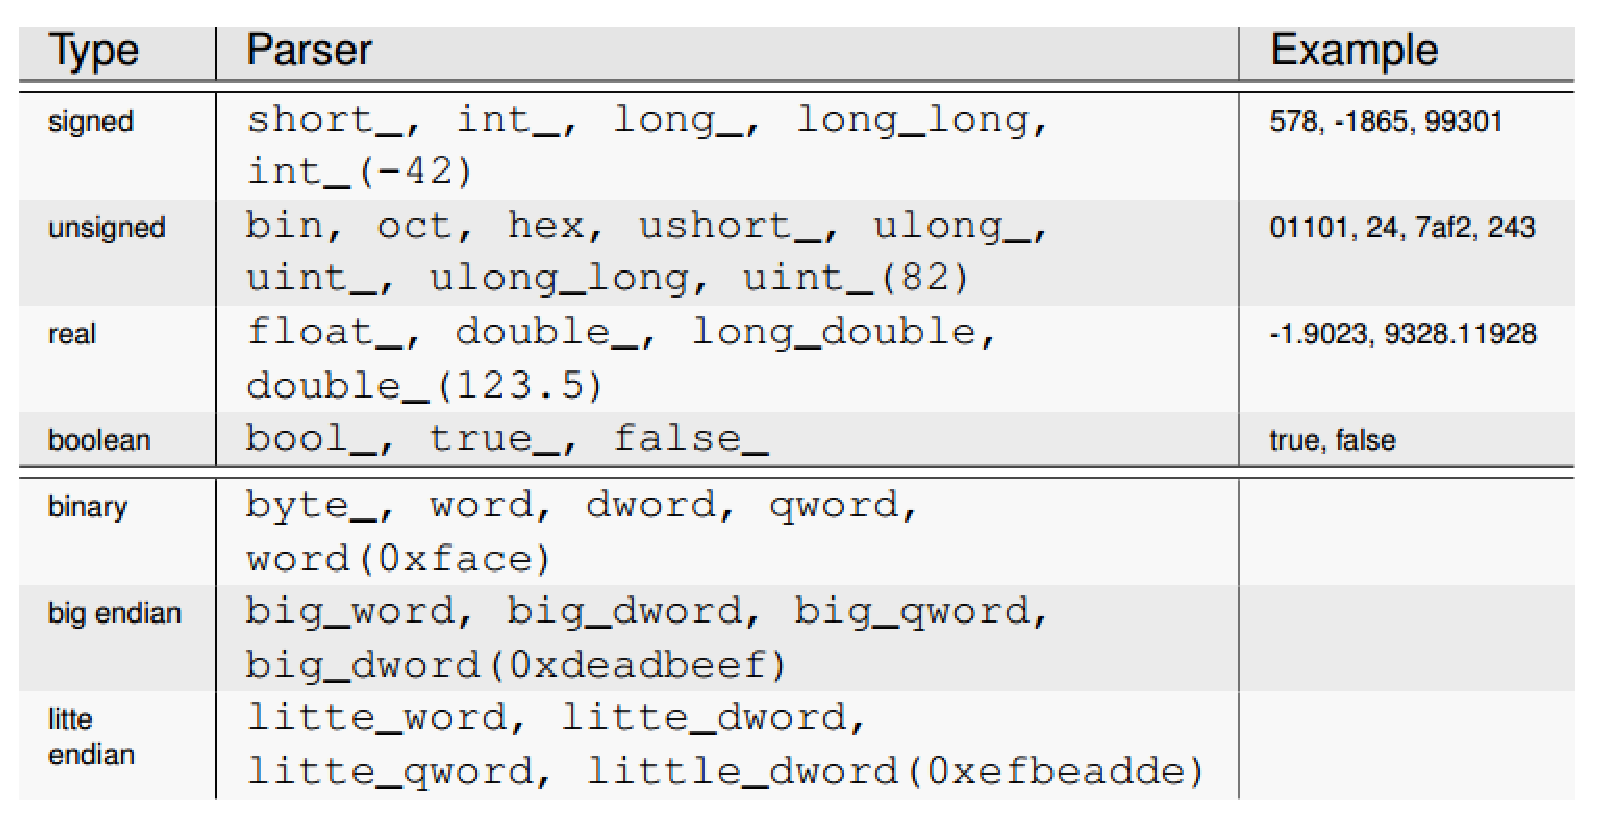
\includegraphics[height=5cm,
    angle=0]{./images/Boost_Spirit_parsers.eps}}
  \centerline{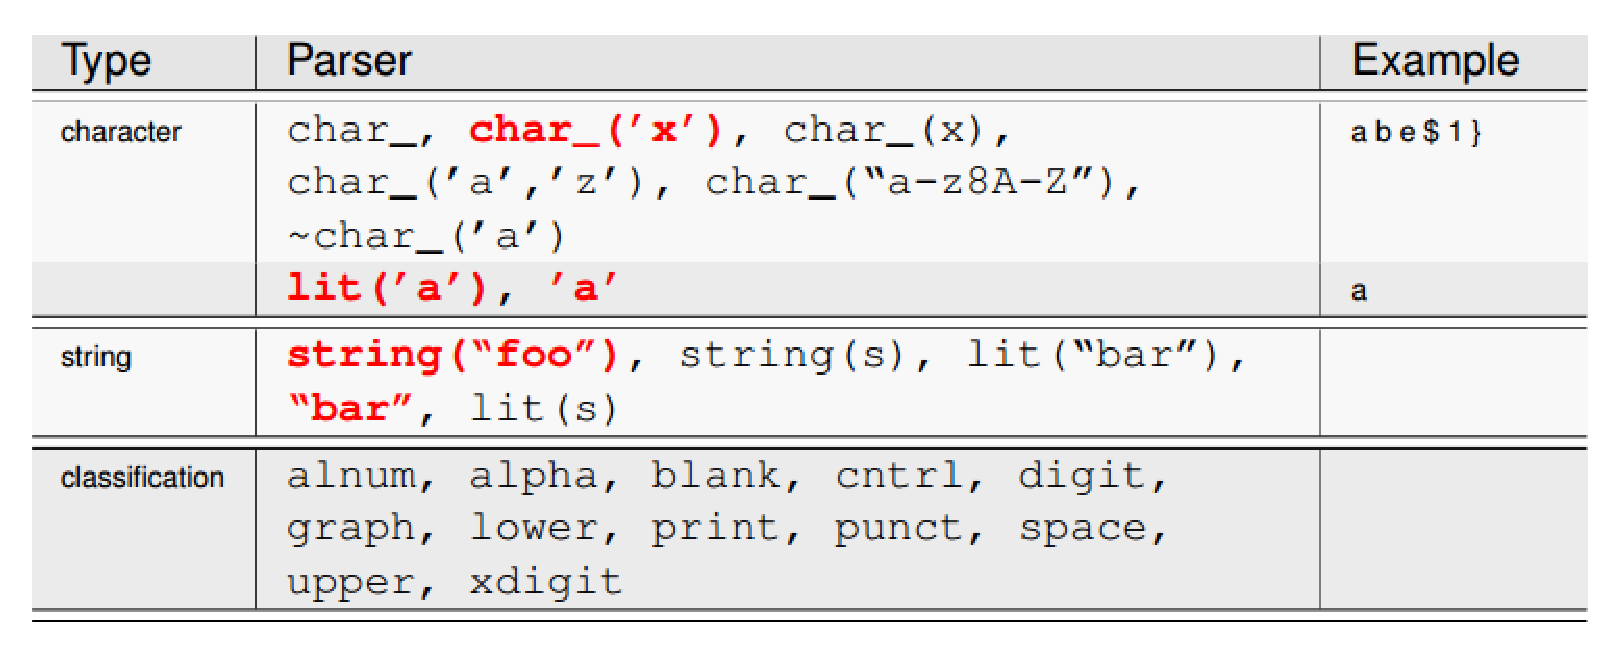
\includegraphics[height=4cm,
    angle=0]{./images/Boost_Spirit_parsers_2.eps}}
  \caption{Available parsers in Spirit::Qi}
  \label{fig:Boost_Spirit_parsers}
\end{figure}

\textcolor{red}{\bf Parsing characters and string need to be careful, due to
different ways to be done, and different character encoding namespace}.  The
possible choices are
\begin{verbatim}
boost::spirit::ascii
boost::spirit::iso8859_1
boost::spirit::standard
boost::spirit::standard_wide
\end{verbatim}
which are also brought into \verb!qi! sub-namespace
\begin{verbatim}
boost::spirit::qi::ascii
boost::spirit::qi::iso8859_1
boost::spirit::qi::standard
boost::spirit::qi::standard_wide
\end{verbatim}
Most of the time, we'll work with \verb!boost::spirit::qi::ascii!.

\textcolor{red}{\bf Character matching}: There are also important notices.
\verb!char_! is a boost::spirit::terminal (grammar[1]) that recognizes a single
character (an alphabet, a numeric, a comma, a dot, etc.), and return the
character as the associated attribute of type \verb!char!. To recognize a single
character, say 'a', we can use \verb!char_("a")!; or a single character (any
one from 'a' to 'z'), we can use \verb!char_("a-z")!. To recognize a single
character, but don't return it to the associated attribute, we use \verb!lit()!
parser.

\begin{verbatim}
//to match a single character, in variable 'ch'
char ch; ch='a';
bool info;

//we have 3 options (but associated attribute can be different)
info = qi::parse("a", ch);
info = qi::parse("a", lit(ch));
info = qi::parse("a", char_(ch));

//to match a single character literal, say 'c'
info = qi::parse('c', char_('c'));

// match any character, e.g. '+', '-' are also character
info = qi::parse('a', char_);
info = qi::parse('b', char_);

// alphabetic only (a-zA-Z)
info = qi::parse('a', alpha) ;

// alphanumeric (a-zA-Z0-9)
info = qi::parse('4', alnum);

//match a string
boost::spirit::qi::lit("some string") ; //string literal parser
\end{verbatim}
with \verb!info! is true for parsing successfully.


NOTE: These primitive parsers can be combined to build more complex parsers
(to be discussed at Sect.\ref{sec:boost_spirit::qi_user_defined_parser}). A good reference
is\footnote{\url{http://boost-spirit.com/home/articles/qi-example/creating-your-own-parser-component-for-spirit-qi/}}

\textcolor{red}{\bf Running the parser is simple}. What we need: (1) an input
string we want to parse, (2) the parser containing the grammar (primitie
parser, a combination of these primitive parsers using operators, or write your
own grammar), (3) calling \verb!qi::parse()! which returns the
successful/failure information of the parsing process. Example: \verb!qi::parse!
API to call the parser \verb!qi::int_!, using the input data given by 2
iterators.

\begin{verbatim}
using namespace boost::spirit;

boost::spirit::parse_info<> info;
std::string input( "1234" );
std::string::iterator iter = input.begin();
std::string::iterator end_iter = input.end();

info = qi::parse( iter, end_iter, int_ );
\end{verbatim}

Example: Another example using \verb!qi::parse! to call the parser
\verb!qi::double_!
\begin{verbatim}
std::string input( "1234.56" );

...
qi::parse( iter, end_iter, double_ );
\end{verbatim}

\verb!parse()! is called on the returned parser instance. Also, the parser
instance additionally exposes its attribute type
\begin{verbatim}
namespace boost { namespace spirit { namespace traits
{
    template <typename Component, typename Context = unused_type
      , typename Iterator = unused_type>
    struct attribute_of;
}}}
\end{verbatim}
\url{http://boost-spirit.com/home/2010/01/31/what-is-the-attribute-type-exposed-by-a-parser/}

\subsection{Skip parser}
\label{sec:skip_parser}

A $skip$ parser is a parser that is used to help tokenize the input by deciding
what is not relevant. So, any thing can be recognized by the $skip$ parser is
not recorded to the semantic actions, except those put into \verb!lexeme [...]!
rule. Usually, the $skip$ parsers skips space and comments. There are two
standard $skip$ parsers:
\begin{verbatim}
boost::spirit::ascii::space
boost::spirit::ascii::space_type
\end{verbatim}
\textcolor{red}{IMPORTANT: The $skip$ parser must be passed right after the
grammar instance, and then comes to the parser assiciated attribute instance
where you keep the parsed result.}

The $skip$ parser is called before each individual subparser.
Example:
\begin{lstlisting}
template <typename Iterator>
struct sequence : boost::spirit::qi::grammar< Iterator,
std::pair<std::string, std::string>(),
boost::spirit::qi::ascii::space_type >
{
        sequence() : sequence::base_type(start)
        {
                start %=
                        literal_ >> literal_
                        ;

                literal_
                        = *(boost::spirit::ascii::alnum | '_')
                        ;
        }
        boost::spirit::qi::rule<Iterator, std::pair<std::string,
std::string>(), boost::spirit::ascii::space_type > start;
        boost::spirit::qi::rule<Iterator, std::string(),
boost::spirit::ascii::space_type > literal_;

};

int main()
{
        grammar sequence_parser;
        std::pair<std::string,std::string> v;
        std::string line = "abc xyz";
        phrase_parse(line.begin(), line.end(), sequence_parser,
boost::spirit::ascii::space, v);
        std::cout << v.first << ", " << v.second << std::endl;
}
\end{lstlisting}


Example: Define a $skip$ parser that ignore comment in the form of 
\begin{verbatim}
// anything to end-of-line
\end{verbatim}
then
\begin{verbatim}	
ascii::space | "//" >> *(char_ - eol) >> eol;
\end{verbatim}


To define  a $skip$ parser, we can define it as a child of \verb!qi::grammar!
too
\begin{verbatim}
using boost::spirit;

template<typename Iterator>
struct pl0_skipper : public qi::grammar<Iterator> {

    pl0_skipper() : pl0_skipper::base_type(skip, "PL/0") {
        skip = ascii::space | ('{' >> *(qi::char_ - '}') >> '}');
    }
    qi::rule<Iterator> skip;
};

template<typename Iterator, typename Skipper = pl0_skipper<Iterator>>
struct pl0_grammar : public qi::grammar<Iterator, Skipper> {

    /* The rules use our skipper */
    qi::rule<Iterator, Skipper> start;
    qi::rule<Iterator, Skipper> block;
    qi::rule<Iterator, Skipper> statement;

};
\end{verbatim}
\url{http://stackoverflow.com/questions/8521314/custom-skip-parser-with-boostspirit}

When we use a $skip$ parser, we need to call
\verb!boost::spirit::qi::phrase_parse()! and pass the $skip$ parser instance as
the last argument
\begin{verbatim}
typedef std::string::const_iterator iterator_t;
typedef parser::pl0_grammar<iterator_t> grammar;
typedef parser::pl0_skipper<iterator_t> skipper;

grammar g;
skipper ws;

iterator_t iter = str.begin();
iterator_t end = str.end();
bool r = phrase_parse(iter, end, g, ws);
\end{verbatim}


\subsection{Unary Parsers}
\label{sec:unary_parsers}

\verb.!p. and \verb!~p! with $p$ is the parser. 

If the component $p$ parsed successfully, then \verb.!p. and \verb.~p. fail. If
$p$ fails, then \verb.!p. and \verb.~p. succeed. IMPORTANT: The unary operator
\verb.~. is applicable to character and character class parsers only.
\begin{verbatim}
~char_	does not match anything
~digit	matches everything except digits
~char_("a-z")   matches every character outside the character range spanned by
                'a' and 'z'
\end{verbatim}
 
While the unary operator \verb.!. is creating a not-predicate parser, i.e. it
doesn't move the current input position forward (or it doesnt consume any
input). It's mainly used to check if a word is a keyword or not, e.g. \verb!for!
is a keyword, but if there is 'now' after that, i.e. \verb!for now!, it is not.

\url{http://boost-spirit.com/home/2010/01/17/whats-the-difference-between-qis-and/}

\subsection{A parser with associated attribute}
\label{sec:associate_attribute}

Each parser has an associated attribute. To extract the data from the parser, we
use this associated attribute. For each parser, it has its own assiciated
attribute type, but we can also use compatible type
(Sect.\ref{sec:associate_attribute_compatible-type})
\begin{enumerate}
  \item \verb!char_! : type is \verb!char!, with \verb!std::string! is a
  compatible type
  \item \verb!hex!: type is \verb!int!
  \item \verb!int_!: type is \verb!int!
  \item \verb!double_!: type is \verb!double!
  \item \verb!*double_!: type is \verb!std::vector<double>!
\end{enumerate}
Interestingly, if parser $p$ has attribute of type A, then parser \verb!*p! has
an attribute of type \verb!std::vector<A>!.

When you define your own grammar, try to avoid the automatic attribute
generation entirely, but use {\bf semantic actions} to manually construct your
own associate type. Semantic action can attach to any point in the grammar
specification. A sementic action can be a plain function or a function object
that is called whenever the part of the parse succesffully recognize a token,
e.g. a parser $p$ and a C++ function $F$, then the expression (in the grammar)
\begin{verbatim}
p[F] 
\end{verbatim}
link $F$ to $p$. Section \ref{sec:semantic_action} describes how to define this
$F$ function for a parser.



\subsection{Semantic actions with parsers}
\label{sec:semantic_action}

NOTE: All Qi, Karma, and Lex - support semantic actions. However, there are
some differences in using for each case. Here, we focus on Qi
\footnote{\url{http://boost-spirit.com/home/2010/03/03/the-anatomy-of-semantic-actions-in-qi/}}.

We can use different ways to link a semantic action to a parser:
\textcolor{red}{global} plain functions, function object, \verb!Boost.Bind!,
\verb!Boost.Lambda!, or \verb!Boost.Phoenix!.  Simplicity, a semantic action is
a callable object that is executed on successful recognition of the token.

NOTE: All these placeholders are available from the namespace 
\verb!boost::spirit::qi!. The latter three allow you to use special place
holders to control parameter placement, i.e.
\begin{enumerate}
  \item Boost.Bind: we use \verb!_1!, \verb!_2!, etc. to represent the $N$-th
  attribute of a parser $p$. It means that a parser can have more than one
  attributes.
  \item Boost.Lambda we use the placeholders defined in \verb!boost::lambda!.
  \item Boost.Phoenix, we use the placeholders defined in the namespace
  \verb!boost::spirit!.
  \begin{itemize}
    \item we use \verb!_1!, \verb!_2!, etc. to represent the $N$-th
  attribute of a parser $p$. It means that a parser can have more than one
  attributes.
    \item \verb!_pass! : if we assign \verb!false! to \verb!_pass!, then it
    forces the generator to fail, regardless of the grammar.
    
    \item \verb!_val!: the synthesized attribute of the associated rule
    \item \verb!_r1, _r2, \ldots, _rN!: the $N$-th inherited attribute of the
    associated rule
    \item \verb!_a, _b, \ldots, _j!: the local variables of the associated rule
    (with \verb!_a! refers to the first one)
  \end{itemize} 
\end{enumerate}
\textcolor{red}{It's recommended to use Boost.Phoenix}.

Example: when using \verb!_1, _2!, as the resulting of whole parsing process
with \verb!qi::_1! refers to the attribute matched by the first integer parser,
and \verb!qi::_2! to the second one.
\begin{verbatim}
std::string input("1234,2345");
std::string::const_iterator begin = input.begin();
std::string::const_iterator end = input.end();
qi::parse(begin, end,
    (qi::int_ >> ',' >> qi::int_)
    [
        std::cout << "Matched integers: "
              << qi::_1 << " and " << qi::_2 << "\n";
    ]
);
\end{verbatim}
This to avoid the case when expected execution can occur, when using this 
\begin{verbatim}
qi::parse(begin, end,
    (qi::int_[f1] >> ',' >> qi::int_[f2])
\end{verbatim}
which execute \verb!f1! when the integer is detected, regardless of whether the
second integer is detected or not.

The signature of a plain function (or function object)  depends on the type of
the parser to which it is attached. Generally, a plain function (or function
object) can take upto 3 parameters
\footnote{\url{http://stackoverflow.com/questions/3066701/boost-spirit-semantic-action-parameters}}:
\begin{enumerate}
  \item the matched attribute type, i.e. the value to be returned when a token
  is matched by the parser
  \item parser context, i.e. the \verb!qi::phoenix! interface, which is useful
  if the semantic action attaches to somewhere to the right hand-side of a rule.
  
  \item a reference to a boolean 'hit' parameter (the match flag, i.e. to
  manipulate the match state)
\end{enumerate}
Typically, we only define a function with one parameter, which represent the
value of the associate attribute type
\begin{verbatim}
// double_ parser, then 
void F(double n)
\end{verbatim}



To link an action, when a token is detected from a parser, we put them inside
[  ]
\begin{verbatim}
parse(first, last, '{' >> int_[&print] >> '}');

parse(first, last, '{' >> int_[print_action()] >> '}');


// A plain function
    void print(int const& i)
    {
        std::cout << i << std::endl;
    }
    
// A function object
// which requires defining operator()
// with function objects, we need to have an operator() with 3 arguments. Since
// we don't care about the other two, we can use unused_type for these. We'll
// see more of unused_type elsewhere. unused_type is a Spirit supplied
// support class.

 struct print_action {
        void operator()(int const& i, qi::unused_type, qi::unused_type) const
        {
            std::cout << i << std::endl;
        }
    };    
\end{verbatim}

Example: calling a member function using Boost.Phoenix
\begin{verbatim}
struct foo{ 
   void f(int ) {...}
}


foo a_f;

//pass to the parser 'p'
// here a_f.f(qi::_1) is called

p[phoenix::bind(&foo::f, a_f, qi::_1)]
\end{verbatim}

Example: calling a member function using Boost.Bind
\begin{verbatim}
// A member function
    struct writer
    {
        void print(int const& i) const
        {
            std::cout << i << std::endl;
        }
    };
    
    
writer w;
parse(first, last, '{' >> int_[boost::bind(&writer::print, &w, _1)] >> '}');

// or we can assign to a member variable, then we don't need to call a function
// but just assignment
std::string input( "12 * 8" );

rule<iter_t, int(), space_type> mult =
int_ [ _val = _1 ]
>> '*'
>> int_ [ _val *= _1 ]
;
\end{verbatim}

\subsection{Simple user-defined parsers}
\label{sec:boost_spirit::qi_user_defined_parser}

We can combine primitive parsers using the operator as shown in
Fig.\ref{fig:boost_spirit::qi_operators}. 

Example: the string to be parsed in the form of 'an integer' + spaces +
'a double'. Here, we use \verb!>>! to combine parsers. 
\begin{verbatim}
std::string input( "876 1234.56" );
std::string::iterator iter = input.begin();
std::string::iterator end_iter = input.end();

bool infor = boost::spirit::qi::parse( iter, end_iter,
         int_ >> ' ' >> double_ );
\end{verbatim}

Example: Matching \verb!{0xbeef}! as 48879 using
\begin{verbatim}
char_('{') >> string("0x") >> hex >> char_('}')
\end{verbatim}


\begin{enumerate}
  \item  'a >> b' is read as '$a$ is followed by $b$'.
  \item 'a > b' means a must be followed by 'b'
  \begin{verbatim}
  char_('o') > char_('k')
  \end{verbatim}
  This rule expects 'ok'. Otherwise, \verb!expectation_failure<iter>! is thrown.
  
  \item 'a | b' is read as either $a$ or $b$ is allowed
  \item '-a' means zero-or-one time occurence of 'a'
  \item '*a' means zero-or-any time occurence of 'a'
  \item '\&a' just provide a basic look-ahead, but not consuming 'a'
  \begin{verbatim}
  #include <boost/spirit/include/qi_and_predicate.hpp>
  
  using boost::spirit::lit;
  test_phrase_parser("Hello ;", lit("Hello") >> &lit(';'), false);
  \end{verbatim}
  
  \item  '!a' provides a basic look-ahead, but not consuming the match in the
  return, e.g. the rule
  \begin{verbatim}
  // 'for' >> !(alnum | '_')  
  \end{verbatim}
  is designed to catch the 'for' keyword. So, the string \verb!for()! is okay,
  but \verb!forty! gives an error to the parser.
  
  
  \item 'a-b' means match 'a' but not 'b'. This is used to detect a
  C-style comment
  \begin{verbatim}
"/*"
>> *(char_ - "*/")
>> "*/"
  \end{verbatim}
  As \verb!char_! is a greedy parser, it accepts any type of characters,
  including \verb!*/!. So to stop when seeing \verb!*/!, we meed use 
  \verb!char_ - ``*/''!.
  
  
  \item 'a \% b' is used to detect a list, with 'b' is the separator (a short
  cut for a >> *( b >> a )). Example: to match the list ``9,2,42,-187,76'', we
  use
  \begin{verbatim}
  int_ % ','
  \end{verbatim}
  
  \item 'a \^{} b' means 'a' and 'b' can be in any order, but each element can
  occur 0:1 times
\end{enumerate}

\begin{figure}[hbt]
  \centerline{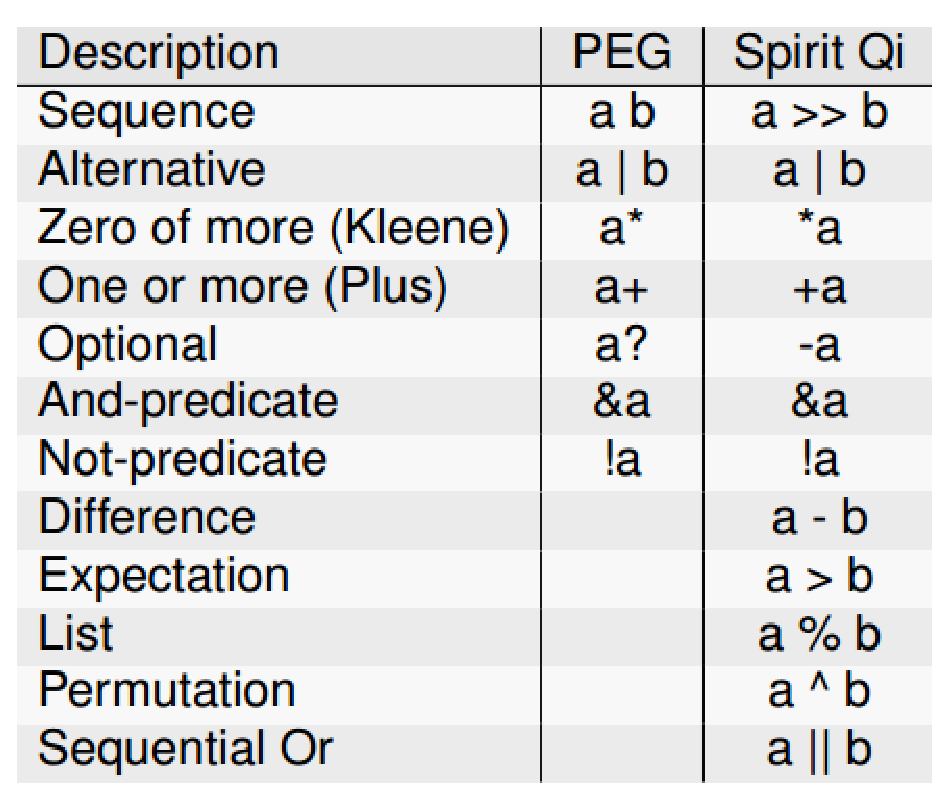
\includegraphics[height=6cm,
    angle=0]{./images/Boost_Spirit_operators.eps}}
  \caption{PEG (Parsing Expression Grammar) and its equivalent form in
  boost::spirit::qi}
  \label{fig:boost_spirit::qi_operators}
\end{figure}

Example: Write a parser that can detect a multi-line string, each line is the
form 'word : word'. Whenever we use \verb!phrase_parse()!, we need to provide a
$skip$ parsers as the last-argument, e.g \verb!space! is the skip parser here

\begin{verbatim}
#include <boost/spirit/include/qi_parse.hpp>

// the input string
std::string input( "foo : bar "
    "gorp : smart "
    "falcou : \"crazy frenchman\" "
    "arm8 : risc " );

// two iterators
std::string::iterator iter = input.begin();
std::string::iterator iter_end = input.end();

boost::spirit::qi::phrase_parse( iter, iter_end,
// ------ start parser -------
*( (alpha >> *alnum)
>> ':'
>> ('"' >> *( ~char_('"') ) >> '"')
|
(alpha >> *alnum)
)
// ------- end parser --------
, space );
\end{verbatim}

However, so far we haven't discussed how to retrived the information from the
input string, when the parsing is successful.


Example: We can define rules to simplify the parser passed to the
\verb!phrase_parse()! command. Consider the example above:
multiple lines, each with \verb!keyword: value! form. We use \verb!qi::rule! to
define the grammar, and parse the input string using \verb!parse_phrase()!.
Here, \verb!space_type! is the $skip$-parser.

\begin{verbatim}
qi::rule<iter_t, space_type> name;
name = alpha >> *alnum;

qi::rule<iter_t, space_type> quote;
quote = '"' >> *( ~char_('"') ) >> '"';
\end{verbatim}
Here, the rule needs an iterator \verb!iter_t!, and a skipper type to be used by
the rule \verb!space_type!.
\begin{verbatim}
std::string input( "foo : bar "
				"gorp : smart "
				"falcou : \"crazy frenchman\" "
				"arm8 : risc " );

typedef std::string::iterator iter_t;
iter_t iter = input.begin();
iter_t iter_end = input.end();

rule<iter_t, space_type> name = alpha >> *alnum;
rule<iter_t, space_type> quote = '"'
			>> *(~char_('"'))
			>> '"';

phrase_parse( iter, iter_end,
		// ------ start parser -------
	*( name >> ':' >> ( quote | name ) )
		// ------- end parser --------
		, space );
\end{verbatim}


%\cprotect\subsection[Using grammar class]{Using \verb!grammar! class} 
\subsection{Using 'grammar' class}

In the case the grammar is quite complicated, you can create your own parser as
a child of the \verb!boost::spirit::qi::grammar! class and using \verb!rule!
inside the grammar.

You should write your grammar first in PEG (Parsing Expression Grammar) which is
easy to understand. PEG is well-suited for parsing computer language, but not
for natural languages
\footnote{\url{http://en.wikipedia.org/wiki/Parsing_expression_grammar}}.

\begin{verbatim}
#include <boost/spirit/include/support_utree.hpp>
#include <boost/spirit/include/qi.hpp>
#include <boost/spirit/include/phoenix_core.hpp>
#include <boost/spirit/include/phoenix_operator.hpp>
#include <boost/fusion/include/adapt_struct.hpp>
#include <boost/assert.hpp>
#include <iostream>
#include <string>
#include <cstdlib>

using boost::spirit::qi;

template <typename Iter>
struct MyGrammar : grammar<Iter, space_type>
{
 //start = name of the starting rule
  MyGrammar() : MyGrammar::base_type(start)
  {
    start = *item;
    item = key >> ':' >> value;
    key = alpha >> *alnum;
    value = ('"' >> *(~char_('"')) >> '"')
            |
            *alnum;
  };

  rule<Iter, space_type> start;
  rule<Iter, space_type> item;
  rule<Iter, space_type> key;
  rule<Iter, space_type> value;
  
};   // IMPORTANT: Don't forget the semicolon here
\end{verbatim}

Now, we  can parse the input string, using \verb!space! as the $skip$ parser.
\begin{verbatim}
int main() {
  std::string input( "foo : bar "
		"gorp : smart "
		"falcou : \"crazy frenchman\" "
		"arm8 : risc " );

  typedef std::string::iterator iter_t;
  iter_t iter = input.begin();
  iter_t iter_end = input.end();

  MyGrammar<iter_t> list_grammar;

  boost::spirit::qi::phrase_parse( iter, iter_end,
        list_grammar,
        space );
		
}
\end{verbatim}



\subsection{Action: Get parsed results}

What if we want to get the parsed results, i.e. we want to keep a list of
'key' and its associated 'value'. That is we need to use the attribute type
associated with each parsers, Fig.\ref{fig:boost_spirit_qi_attribute-type}. The
argument(s) to \verb!parse()! or \verb!parse_phrase()! counting from the
fourth-argument to the one before the last argument, returns the value(s) of the
attribute type associated with the parser.  

Example: here, we use two variables to save the attribute values for two
parsers.

\begin{verbatim}
std::string input( "cosmic pizza" );
std::string::iterator iter = input.begin();
std::string::iterator end_iter = input.end();
std::string result1;
std::string result2;

boost::spirit::qi::parse( iter, end_iter,
		*(~char_(' ')) >> ' ' >> *char_,
		result1,
		result2 );

\end{verbatim}



If you look at the way a parser is defined, the second template type, i.e. T, is
the type of the attribute.
\begin{verbatim}
template <typename P, typename T>
MyGrammar : qi::grammar<P, T> 
{
  ...
}
\end{verbatim}

\begin{figure}[hbt]
  \centerline{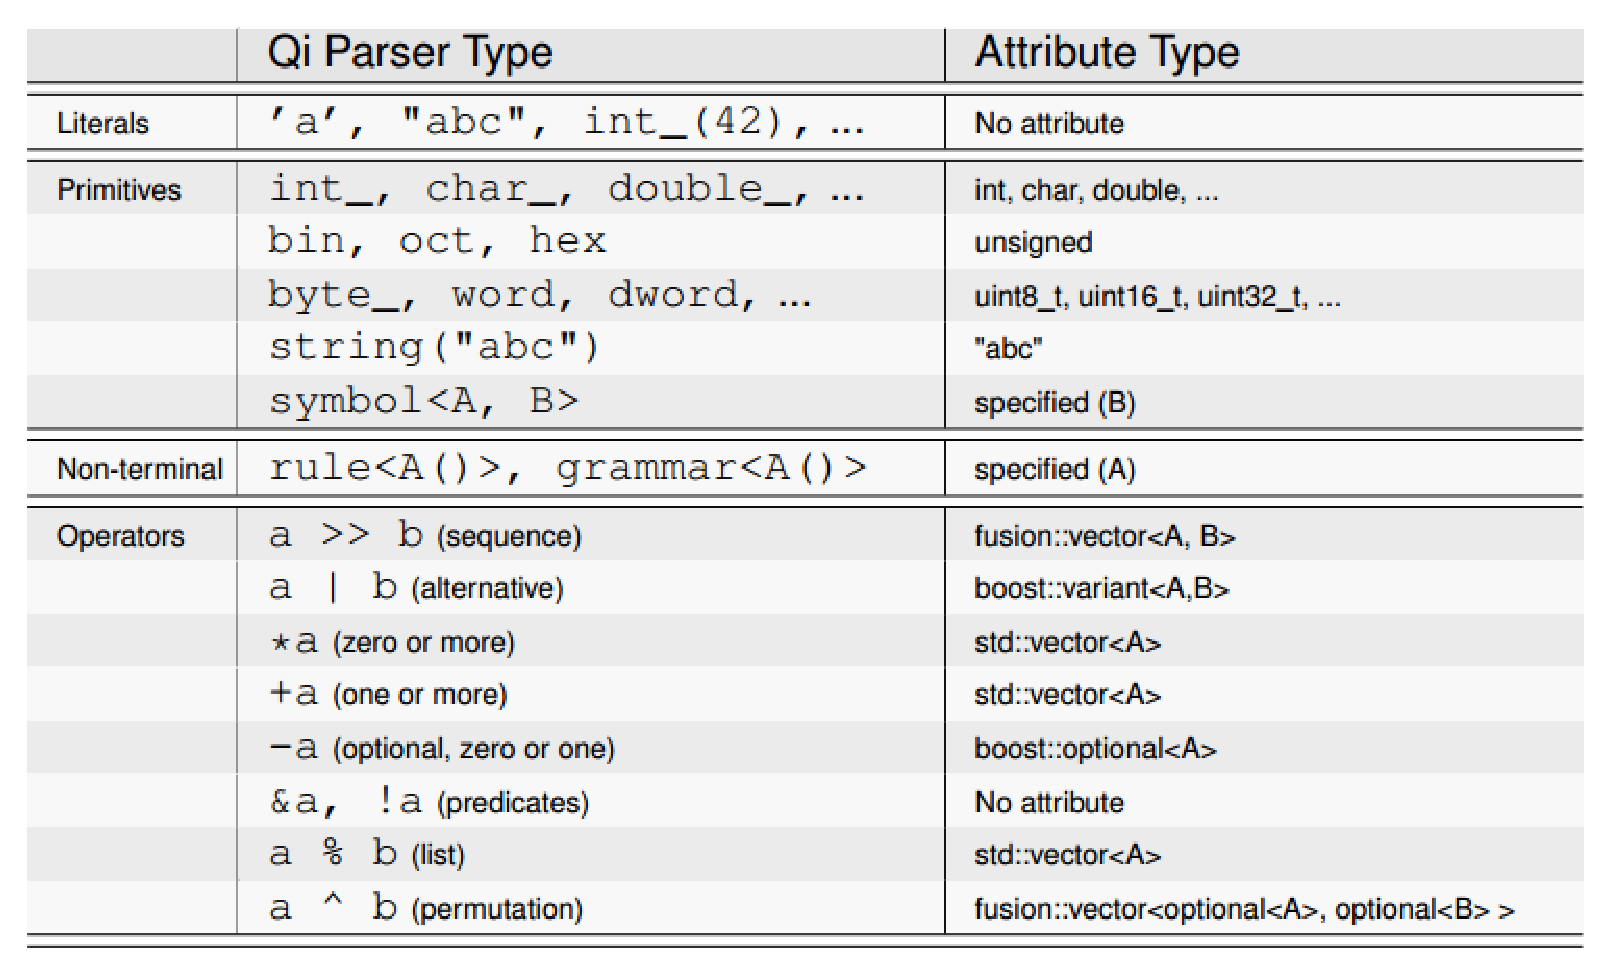
\includegraphics[height=7cm,
    angle=0]{./images/Boost_Spirit_attribute-type.eps}}
\caption{Attribute type associated with primitives parsers}
\label{fig:boost_spirit_qi_attribute-type}
\end{figure}

\subsubsection{Return integer}
 
A simple example below return the integer value of the string, if parsing is
successful.
\begin{verbatim}
std::string input( "1234" );
std::string::iterator iter = input.begin();
std::string::iterator end_iter = input.end();
int result;
parse( iter, end_iter,
        int_,
        result );
\end{verbatim}

NOTE: Compatible attribute type can also be used to get the result, e.g
std::string is compatible with std::vector<char>
attribute of the \verb!*char_! parser.
\begin{verbatim}
std::string input( "pizza" );
std::string::iterator iter = input.begin();
std::string::iterator end_iter = input.end();
std::string result;
parse( iter, end_iter,
		*char_,
		result );
\end{verbatim}

\subsubsection{Return a pair of strings}

If the grammar contains of 2 types of token, we can use more than one parsers
(separated by \verb!>>!, and extract the string value from each parser by using
more than one variable , to get the corresponding associated attrubute
\begin{verbatim}
std::string input( "cosmic pizza" );
std::string::iterator iter = input.begin();
std::string::iterator end_iter = input.end();
std::string result1;
std::string result2;

boost::spirit::qi::parse( iter, end_iter,
		*(~char_(' ')) >> ' ' >> *char_,
		result1,
		result2 );
\end{verbatim}
Here \verb!result1! keep the value for \verb!*(~char_(' '))!, the attribute for
' ' is \verb!unused! or it has no attribute, and \verb!result2! keeps the value
for \verb!*char_!. 

If we want to use $skip$ parser, we need to make sure the white space is not
removed before exttracting the tokens.
\begin{verbatim}
// with skip parser, we don't need to use ' ' token.
// However, you will get unexpected result here
// as result1 keep the 2 words without spaces between 
// and result2 is empty
boost::spirit::qi::phrase_parse( iter, end_iter,
		*(~char_(' ')) >> ' ' >> *char_, ascii:space_type
		result1,
		result2 );

// to resolve the issue
// the solution is lexeme[ ... ]
// any space between will not be removed before applying the sub-parser
boost::spirit::qi::phrase_parse( iter, end_iter,
		lexeme[*(~char_(' '))] >>  *char_, ascii:space_type
		result1,
		result2 );
\end{verbatim}

\subsubsection{Return a vector of strings}

\subsubsection{Return a map of <string, string>}

Again, the two string can be compatible to a map of two string. 
\begin{verbatim}
std::pair<std::string, std::string> result;
parse( iter, end_iter,
		*(~char_(' ')) >> ' ' >> *char_,
		result );
\end{verbatim}

Example: put into the vector
\begin{verbatim}
std::list<int> list;

void got_it (int n) { list.push_back (n); }

*('{' >> lit("0x") >> hex[&got_it] >> '}'))
\end{verbatim}
The idea is simple: when a hexadecimal number is recognized, call a function
which pushes the number onto a list"
\footnote{\url{http://climbing-the-hill.blogspot.com/2010/05/boost-your-spirits.html}}.

Example: Here, we use <map>
\begin{verbatim}
std::map< std::string, std::string > key_value_map;

std::string input( "foo : bar ,"
				"gorp : smart ,"
				"falcou : \"crazy frenchman\" " );

typedef std::string::iterator iter_t;
iter_t iter = input.begin();
iter_t iter_end = input.end();

rule<iter_t, std::string(), space_type> name = alpha >> *alnum;
rule<iter_t, std::string(), space_type> quote = '"'
				>> lexeme[ *(~char_('"')) ]
				>> '"';
rule<iter_t, std::pair<std::string, std::string>(), space_type>
			item = name >> ':' >> ( quote | name );

std::map< std::string, std::string > key_value_map;

phrase_parse( iter, iter_end,
			item % ',',
			space,
			key_value_map );
\end{verbatim}
NOTE: How the starting rule \verb!item! has the associated attribute type of
\verb!std::pair<std::string, std::string>()!, and its two sub-rules \verb!name!
and \verb!quote! has the associated attribute types as \verb!std::string()!.

Example: Fig.\ref{fig:Boost_Spirit_example_1} also include the printint out
parsed result using \verb!std::for_each! loop. \textcolor{red}{QUESTIONS: What
is }\verb!phx::at_c<0>(arg1)!
\footnote{\url{http://www.boost.org/doc/libs/1_46_1/libs/fusion/doc/html/fusion/adapted/std__pair.html}}.
\verb!at_c<N>(seq)! returns the $N$-th element from the beginning of the
sequence.

\begin{verbatim}
std::pair<int, std::string> p(123, "Hola!!!");
std::cout << at_c<0>(p) << std::endl;
std::cout << at_c<1>(p) << std::endl;
std::cout << p << std::endl;

vector<int, int, int> v(1, 2, 3);
assert(at_c<1>(v) == 2);
\end{verbatim}


\begin{figure}[hbt]
  \centerline{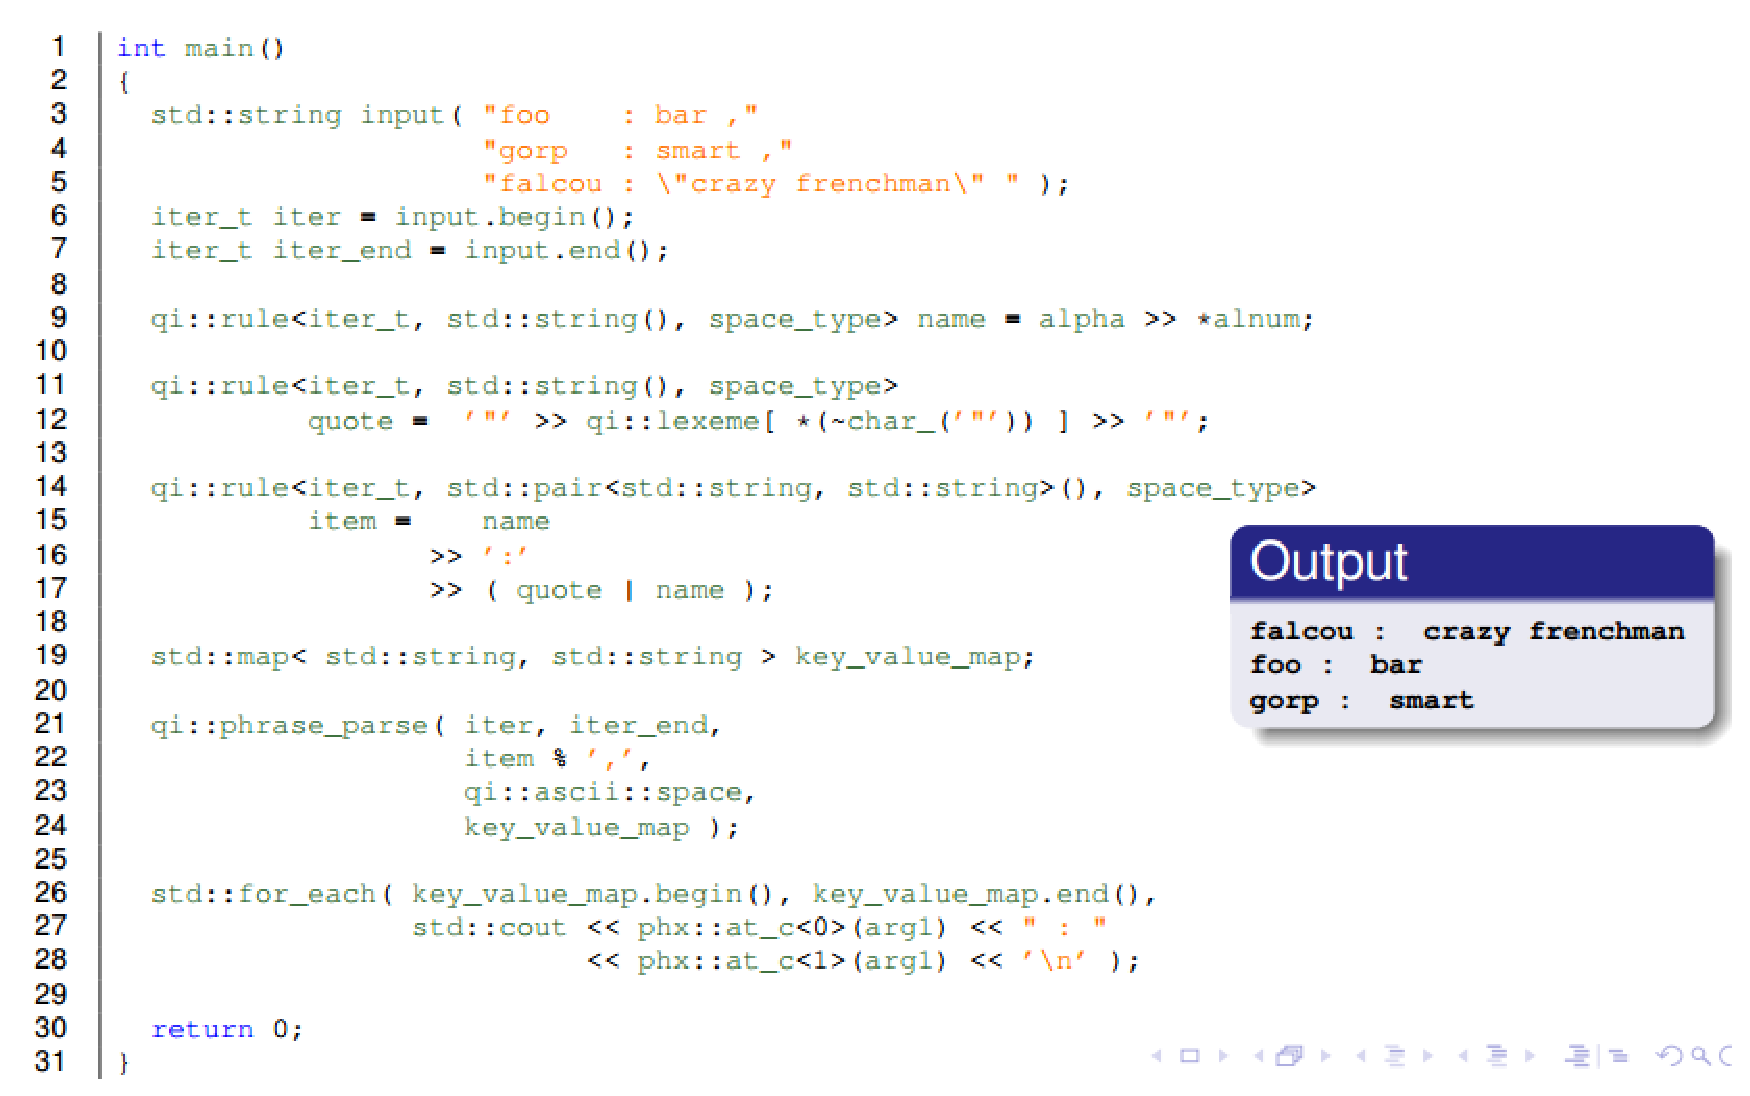
\includegraphics[height=8cm,
    angle=0]{./images/Boost_Spirit_example_1.eps}}
\caption{A complete example of using Boost::spirit::qi}
\label{fig:Boost_Spirit_example_1}
\end{figure}

\subsubsection{Return a struct}

There are two ways: the not-a-smart-way is to create a struct with a
proper construction. The second way is discussed in the next section, using
Boost.Fusion.

\subsubsection{Return a struct (using Boost.Fusion)}


First we create a struct that we want to store the parsed data
\begin{verbatim}
namespace myclient {
  struct employee
  {
  int age;
  std::string firstname;
  std::string lastname;
  double salary;
//  std::map<std::string, std::string> some_record;
  }
}
\end{verbatim}
NOTE: The problem of using a comma (,) in the type, which when pass to macro
expansion it can give you errors like
\begin{verbatim}
macro "BOOST_FUSION_ADAPT_STRUCT_FILLER_0" passed 3 arguments, but takes just 2
\end{verbatim}
when you do something
\begin{verbatim}
BOOST_FUSION_ADAPT_STRUCT(TestStruct, (int, myint)(double, mydouble)
       (std::pair<std::string, std::string>, some_record));
\end{verbatim}
To resolve this problem, just use \verb!typedef! to define a new name, and then
use the alias name for the data type.
\begin{verbatim}
typedef std::pair<std::string, std::string> my_type_t;

BOOST_FUSION_ADAPT_STRUCT(TestStruct, (int, myint)(double, mydouble)
       (my_type_t, some_record));
\end{verbatim}


Then, at the global namespace, use Boost.Fusion
\begin{verbatim}
BOOST_FUSION_ADAPT_STRUCT(TestStruct, (int, myint)(double, mydouble));
\end{verbatim}

Then, next in the \verb!myclient! namespace, we define
\begin{verbatim}
template <typename Iterator, typename Skipper>
struct MyGrammar : qi::grammar<Iterator, TestStruct(), Skipper> {
    MyGrammar() : MyGrammar::base_type(mystruct) {
        mystruct = qi::int_ >> ":" >> qi::double_;
    }
    qi::rule<Iterator, TestStruct(), Skipper> mystruct;
};
\end{verbatim}

Finally, you can use it
\begin{verbatim}
int main() {
    typedef std::string::const_iterator It;
    const std::string input("2: 3.4");
    It it(input.begin()), end(input.end());

    MyGrammar<It, qi::space_type> gr;
    TestStruct ts;

    if (qi::phrase_parse(it, end, gr, qi::space, ts) && it == end)
        std::cout << ts.myint << ", " << ts.mydouble << std::endl;

    return 0;
}
\end{verbatim}

\subsection{Attribute parsing - compatibility}
\label{sec:associate_attribute_compatible-type}

\begin{verbatim}
a: char, b: std::vector<char> 
  -->  ( a >> b ): std::vector<char>

a: unused, b: vector<char>, c: unused 
  --> ( a >> b >> c): std::vector<char>

a: string, b: string 
  --> ( a | b): variant<string, string> ! string

a: string, b: unused, c: string 
  --> ( a >> b >> c): tuple<string, string>

a: std::pair<string, string> 
  --> ( a % b ): vector< std::pair<string, string> >
    
\end{verbatim}


\subsection{Minimum headers to use}

When we implement the parser
\begin{verbatim}
#include <boost/spirit/include/qi.hpp>
#include <boost/spirit/include/phoenix.hpp>
#include <boost/fusion/include/adapt_struct.hpp>
\end{verbatim}

When we use the parser, we need
\begin{verbatim}
#include <boost/fusion/include/std_pair.hpp>
\end{verbatim}
This is important if your parser using \verb!std::pair< , >!.

\subsection{Detecting error when parsing}

\url{http://boost-spirit.com/home/articles/qi-example/tracking-the-input-position-while-parsing/}



\subsection{C++ preprocessor using Qi::Classic}

\url{http://www.codeproject.com/Articles/3853/Wave-a-Standard-conformant-C-preprocessor-library}

\section{High-order function objects}

To write code more concise, expressive and readable. 

\section{Smart pointers}

Smart pointers provide automatic lifetime management of objects and simplify
resource sharing. This is now part of C++11 

\section{Conversion to containers and data structures}


\section{Regular expression: Boost.Regex, Boost.Tokenizer}

If we have sophisticated text processing, we can use Boost.Regex, 
Boost.Tokenizer, or Boost.Spirit. 

\section{Function objects defined at the call site: Boost.Bind and
Boost.Lambda}

For functional programming, we can use \verb!Boost.Lambda!.

\section{Flexible callbacks: Boost.Function}

\section{Manage signals + slots: Boost.Signals}

\section{Convert text and numbers: Boost.lexical\_cast}

To convert between text and numbers, or between any streamable types, we use
\verb!Boost.lexical_cast!


\section{Math: Boost.Math}
\label{sec:boost_math}


\url{http://www.boost.org/doc/libs/1_53_0/libs/math/doc/html/index.html}

\section{Random: Boost.Random}


\section{Rational number: Boost.Rational}

\section{Complex number: Boost.Quaternion}

Quaternion provides an efficient way to parameterize rotation in 3D and 4D.

\url{http://www.boost.org/doc/libs/1_41_0/libs/math/doc/quaternion/html/}

\section{Multi-dimensional array: Boost.MultiArray}



\section{Graph: Boost.Graph}

\section{Timer/IO utilities: Boost.Chrono}
\label{sec:Boost-Chrono}
\label{sec:Chrono-library}
\label{sec:Boost.Chrono}

\url{http://www.boost.org/doc/libs/1_58_0/doc/html/chrono.html}
\begin{lstlisting}
// Include all of Chrono files
#include <boost/chrono.hpp>

\end{lstlisting}


Some features is now part of C++11 \verb!#include! \verb!<chrono>! - Sect.\ref{sec:chrono-header-file}
   
NOTE: Boost Chrono has I/O, rounding and many other clock utilities that C++11
doesn't have. So, we may still want to use Boost Chrono in these situations.

\section{Utilities}


\begin{verbatim}
#include <boost/utility.hpp>
\end{verbatim}



\subsection{result\_of}
\label{sec:result_of-BOOST}

\verb!boost::result_of<>! =  \verb!std::result_of!

It was introduced in Boost, and then included into C++ TR1, then C++0x, and now
is part of C++11 standard.
In C++11, we can use a similar language feature called \verb!decltype! which is
an entirely new thing in C++0x, does not restrict only to return type of a
function, and is a language feature.

In C++0x, \verb!result_of! is implemented based on \verb!decltype!
\begin{verbatim}
 template<typename _Signature>
    class result_of;

  template<typename _Functor, typename... _ArgTypes>
    struct result_of<_Functor(_ArgTypes...)>
    {
      typedef
        decltype( std::declval<_Functor>()(std::declval<_ArgTypes>()...) )
        type;
    };
\end{verbatim}

\url{https://www.boost.org/doc/libs/1_42_0/boost/utility/result_of.hpp}

The class template \verb!result_of! helps determine the type of a call
expression.
For example, given an lvalue (Sect.\ref{sec:lvalue}) f of type F and lvalues
t1, t2, ..., tN of types T1, T2, ..., TN, respectively, the type
\verb!result_of<F(T1, T2, ..., TN)>::type! defines the result type of the
expression f(t1, t2, ...,tN).

\begin{verbatim}

\end{verbatim}

This implementation permits the type F to be a function pointer, function
reference, member function pointer, or class type.

Boost::\verb!result_of! has, by default, N may be any value between 0 and 16.
To change the upper limit, define the macro \verb!BOOST_RESULT_OF_NUM_ARGS! to the maximum value for N, as defined in 
\verb!boost/utility/result_of.hpp! file.



\begin{verbatim}
//namespace boost

template<typename F> struct result_of;
\end{verbatim}

\section{C++ and other language}

\subsection{Python: Boost.Python}


\chapter{OOMPH-Lib}
\label{chap:OOMPH-Lib}

\section{Introduction}

This is a parallel library for single or multiple-physics simulation. 
The current version is 0.90. The essential third-party packages that comes with
oomph-lib are:
\begin{enumerate}
  \item BLAS: (non-parallel)
  \item LAPACK: parallel implementation of BLAS, EISPACK, and LINPACK
  \item SuperLU: direct-solver for large, sparse, non-symmetric system of linear
  equations on high-performance machines. It performs LU-decomposition with
  partial pivoting and triangular system CAN BE SOLVED using forward and
  backward substitution.
  \item METIS: a set of serial programs for partitioning finite-element meshes,
  and producing fill reducing ordering for sparse matrices. The algorithms
  implemented here are based on multi-level recursive-bisection, multi-level
  $k$-way, and multi-constraint partitioning schemes.
\end{enumerate}

Also, you may want to include to compile with some third-party libraries
\begin{enumerate}
  \item Hypre 2.0.0: Sect.\ref{sec:hypre}

  \item Trilinos 9.0.2: Object-oriented software framework for the solution of
  large-scale, complex multi-physics engineering
  
\end{enumerate}

Scalability involves architecture of the parallel computer, parallel
implementation of the algorithm, and the scalibility of the algorithm itself.
So, it describes how the system required grows with the size of the problem.

In many large-scale scientific simulation codes, the majority of run times is
spent on linear-solver which solve large, sparse linear systems of equations on
parallel computers.

Prerequisites:
\begin{enumerate}
  \item Install doxygen: 1.8.4
  \item Install Hypre: Sect.\ref{sec:hypre}
  \item Triangle: \url{www.cs.cmu.edu/~quake/triangle.html}, which generate
  exact Delaunay triangulations, Voronoi diagrams, constrained Delaunay
  triangulations, conforming Delaunay triangulations, and high-quality
  triangular meshes. The triangular meshes then can be used for finite-element
  analysis. Compile and add to PATH. 
  \item TetGen: generate tetrahedral meshes of any 3D polyhedral domains.
  Compile and add to PATH.
  \item Modify the files in \verb!external_src/oomph-metis-4.0.0/! by renaming
  \verb!log2! into \verb!log2_function!. This is to avoid the name conflict with
  /usr/include/bits/mathcalls.h:145
\end{enumerate}


How to compile-and-install:
\begin{verbatim}

## Make sure /home/minhtuan/local/hypre/ has 2 subdirs: include, lib
## oomph-lib
mkdir /home/minhtuan/local/oomph-lib
./configure --prefix=/home/minhtuan/local/oomph-lib/ \ 
    --with-hypre=/home/minhtuan/local/hypre/
make --jobs=4 2>&1 | tee m.txt
make install 2>&1 | tee mi.txt
\end{verbatim}

How to link your code to use oomph-lib? Demo codes are provided in
\verb!demo_drivers! folder.
\begin{itemize}
  \item set \verb!LIBDIR! to the /home/minhtuan/local/oomph-lib/lib
  \item add \verb!-LLIBDIR! to the compiler option (to be able to compile the
  code that use the oomph-lib)
  \item add \verb!$LIBDIR! to \verb!LD_RUN_PATH! (to be able to link the
  components) or add any of the following \verb!-Wl, --rpath -Wl, LIBDIR!
  linker flag.
  \item add \verb!$LIBDIR! to the environment variable \verb!LD_LIBRARY_PATH!
  (to be able to run the compiled program)
  \item 
\end{itemize}

\textcolor{red}{How to use it?} - See Sect.\ref{sec:oomph-lib_how2use}.

\textcolor{red}{How to analyze the data?} - The post-processing of oomph-lib
produces ASCII-data in a format that can be read-in by {\bf tecplot} - a commercial plotting
package. We can also use {\bf gnuplot} for simple visualization (not 3D). A
python script written by Angelo Simone can convert the output to VTU format that
can be read by {\bf paraview} (Read visualization book on this section).

\section{Poisson equation}

The Poisson equation is very simple, yet has very powerful applications. Given
the function G, solve for $F$ with the property
\begin{equation}
\Delta F = G
\end{equation}
with $\Delta$ is a symmetric linear operator.

This can be used to \footnote{\url{www.cs.jhu.edu/~misha/Fall07/}} 
\begin{enumerate}
  \item FFT
  \item Jacobi/Gauss-Seidel solvers
  \item Conjugate Gradients
  \item Multigrid
  \item Pre-conditioning
\end{enumerate}

We'll focus on its application in smoothing, i.e. removing artifacts/noise from
surface meshes. Given a function $F:\mathcal{R}^2\rightarrow \mathcal{R}$, the
{\bf gradient of F} is the vector field $\nabla F: \mathcal{R}^2 \rightarrow\mathcal{R}^2$ 
defined as the partial derivatives
\begin{equation}
\nabla F(x,y) = \left( \frac{\partial F}{\partial x}, \frac{\partial
F}{\partial y}\right)
\end{equation}
So, at the point $p_o$, the vector $\nabla F(p_o)$ points in the direction of
greatest change of $F$, Fig.\ref{fig:gradient}.


\begin{figure}[hbt]
  \centerline{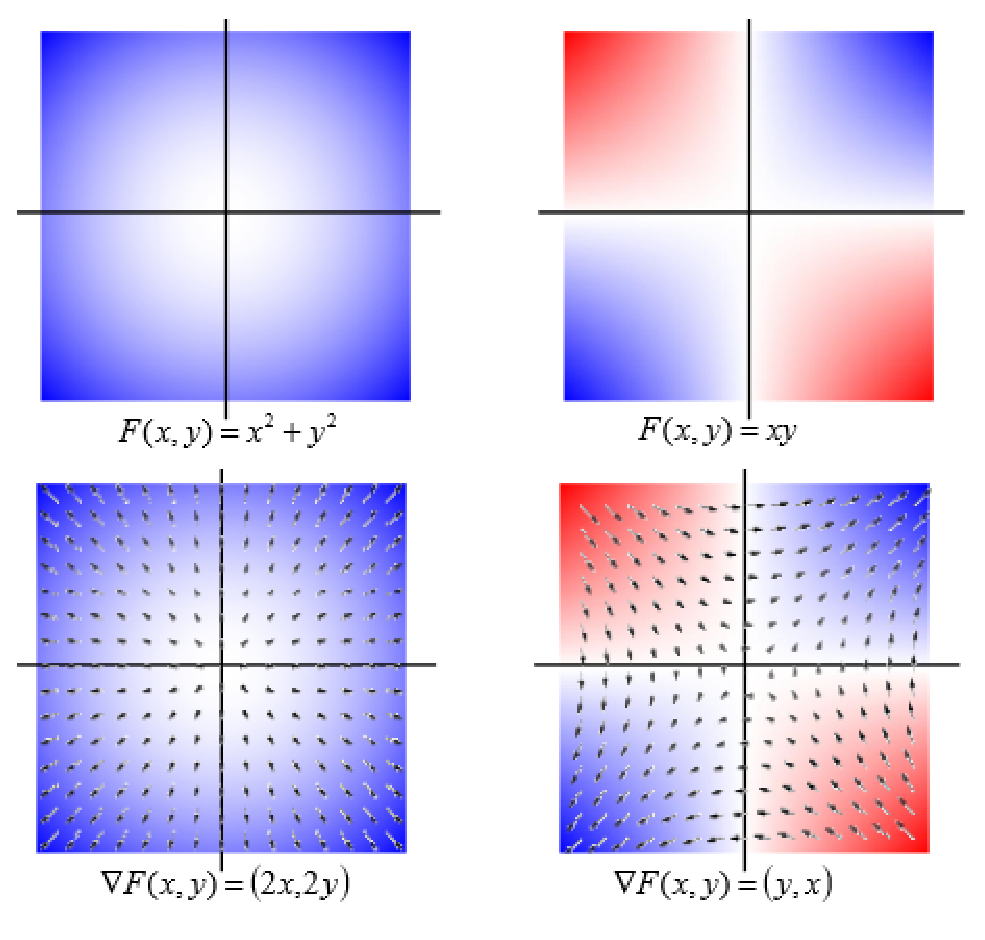
\includegraphics[height=4cm,
    angle=0]{./images/gradient.eps}}
  \caption{The vector fields}
\label{fig:gradient}
\end{figure}

The set of all gradients is called the vector field. Given a vector field
$\vec{F}=(F_1,F_2): \mathcal{R}^2\rightarrow \mathcal{R}^2$, the {\bf divergence
of $\vec{F}$} is the function: $\nabla \cdot \vec{F}: \mathcal{R}^2\rightarrow
\mathcal{R}$, defined by the partial derivatives
\begin{equation}
\nabla \cdot \vec{F}(x,y) = \frac{\partial F_1}{\partial x} + \frac{\partial
F_2}{\partial y}
\end{equation}
So, at the point $p_o$, the divergence $\nabla\cdot F(p_o)$ is a measure of the
extent to which the flow (de)compresses at $p_o$.

{\bf The Laplacian of F} is the function $\Delta F: \mathcal{R}^2\rightarrow
\mathcal{R}$ (or $\nabla^2F$)
\begin{equation}
\Delta F(x,y) = \nabla\cdot\left(\nabla F(x,y) \right) = \frac{\partial^2
F}{\partial x^2} + \frac{\partial^2 F}{\partial y^2}
\end{equation}
So, at the point $p_o$, the Laplacian of F measures the extent to which the
value of F at $p_o$ differs from the average value of $F$ of its neighbors.  

The Laplacian of F can be defined by considering the family of smoothed
functions
\begin{equation}
G(t,x,y) = F(x,y)\star e^{-\left(x^2+y^2\right)/t}
\end{equation}
which satisfies the property: 
\begin{equation}
\frac{\partial G}{\partial t}|_{t=0}=\Delta F
\end{equation}

The function F can be updated to perform a small amount of function smoothing on
the function F
\begin{equation}
F(x,y) \leftarrow F(x,y) + \varepsilon \Delta F(x,y)
\end{equation}





\section{Using oomph-lib}
\label{sec:oomph-lib_how2use}

We define the problem as an object, and then call the appropriate solver. By
default, the problem is assumed to be non-linear and the Newton's method is used
(using Jacobian matrix).

\begin{verbatim}
 main()
        {
          // Create the problem object
          MyProblem problem; 
          
          // Solve the problem, using oomph-lib's default Newton solver
          problem.newton_solve();
        }
\end{verbatim}
The problem is an instance of the {\bf MyProblem} class. So, basically, you need
to write your own class, say MyProblem, which is an inheritance from the generic
{\bf oomph::Problem} class. How much effort to write your own class depends on
the problem. A few member functions need to be implemented
\begin{enumerate}
  \item \verb!MyProblem()!: the constructor
  \item \verb!Problem::actions_before_newton_solve()! and 
\verb!Problem::actions_after_newton_solve()!: two member functions 
\end{enumerate}

To write the constructor, we need to tell
\begin{enumerate}
  \item the time-step: 
  \begin{verbatim}
  Problem::add_time_stepper_pt(new SomeTimeStepper());
  \end{verbatim}
 \item the {\bf Mesh} object (for finite-element simulation):
 Sect.\ref{sec:oomph_mesh}
 \begin{verbatim}
 Problem::mesh_pt() = new SomeMesh<SomeElement>(...);
 \end{verbatim}
 
 \item the boundary condition: (by default) all nodal values are assumed to be
 free and be zero initially. So, for those that are boundary values and/or
 initial values are not zero, then we need to set. For example: node 0 is the
 boundary and is always to be 10, then we 'pin' a value 10 to it
 \begin{verbatim}
 Problem::mesh_pt()->node_pt(0)->pin(0);
 
 // Set the first element (0,) to value 1.0
 Problem::mesh_pt()->node_pt(0)->set_value(0,1.0);
 \end{verbatim}
 NOTE: \textcolor{red}{The first element is zero-th index based on C++
 indexing scheme.}
 
 \item 
\end{enumerate}

and is treated as a set of algebraic
equations of unknown {\bf u} and the parameters $\mathbf{\lambda}$:
$\mathbf{R(u,\lambda)}=0)$.

\subsection{Documentation}

OOMPH-Lib comes with \verb!DocInfo! class which uses ifstream and ofstream to
test if folder for writing exists. However, in BG/Q it doesn't work, then we can
derive a new class which contais the data member to keep the folder name
\verb!Folder!, and the 
\begin{lstlisting}
//cardiac_utilities.h
class CardiacDocInfo
{

private:
  std::string Folder;
  unsigned Number;
public:

  CardiacDocInfo();

  void set_directory(std::string folder);

  std::string& directory();

  unsigned& number();

};
\end{lstlisting}




\subsection{Build Mesh}
\label{sec:oomph_mesh}

\subsection{Example: Poisson 1D}

Poisson problem or Poisson equation has a very broad range of applications in
mechanical engineering, electrostatics, etc. It's a PDE of elliptic type, with
the general form which arises in steady-state heat conduction with distributed
source $\phi$ (temperature), and $\phi(x,y)$ is the stress function:
\begin{equation}
\nabla^2\phi + g = 0
\end{equation}

Example 1:
\begin{equation}
\frac{\partial^2 u}{\partial x^2} = \pm 30\sin(\sqrt{3x})
\end{equation}
with $x\in [0,1]$, and boundary conditions $u(0)=1, u(1)=\mp 1$

Another example is
\begin{equation}
\frac{\partial^2 u}{\partial x^2}= s(x) = 4\pi^2.\sin(\pi x).\cos(\pi x)
\end{equation}
with $x\in [0,1]$, and boundary condition $u(0)=u(1)=0$.

Now, how to represent the PDE as a \verb!Problem! object.
 
\chapter{GMP library}
\label{chap:GMP-lib}

There are two header files that you can choose
\begin{itemize}
  \item C lang: \verb!gmp.h!
  
  \item C++ lang: \verb!gmpxx.h!
\end{itemize}
To make sure GMP support C++, compile with \verb!--enable-cxx! 
\begin{verbatim}
./configure --prefix=~/gmp --enable-cxx
make
make install
\end{verbatim}

In Code
\begin{verbatim}
#include <stdio.h> // required for FILE* parameter

#include <stdarg.h> // required for va_list parameter
                    // e.g. gmp_vprintf()
#include <obstack.h>  // required for 'struct obstack' parameter
                   // e.g. gmp_obstack_printf()
#include <gmp.h> 
\end{verbatim}


Compile: 
\begin{verbatim}
 // 
g++ mycxxprog.cc -lgmp

// GMP C++ functions
g++ mycxxprog.cc -lgmpxx -lgmp
\end{verbatim}

NOTE: If the GMP library is installed to non-standard location, use '-I' and
'-L' compiler options to point to the right directories.

\section{Data type }
\label{sec:GMP-datatypes}

GMP uses a different name for intrinsic data type, e.g. integer usually means a
multiple precision integer.

GMP uses 
\begin{enumerate}
  \item \verb!mpz_t! type for integers with multiple precision
  
  \item \verb!mpq_t! type for rational numbers with multiple precision
  
  \item \verb!mpf_t! type for floating-point numbers with arbitrary precision
  mantissa with a limited precision exponent. 
  
  
  \item \verb!mp_limb_t! type:
  
  A limb means the part of a multi-precision number that fits in a single
  machine word. (We chose this word because a limb of the human body is
  analogous to a digit, only larger, and containing several digits.) Normally a
  limb is 32 or 64 bits. 

  \item \verb!mp_size_t! type: which counts of limbs of a multi-precision
  number. Currently this is normally a long, but on some systems it's an
  \verb!int! for efficiency, and on some systems it will be \verb!long long! in
  the future.
  
  \item \verb!mp_bitcnt_t! type: which counts of bits of a multi-precision
  number. Currently this is always an \verb!unsigned long!, but on some systems
  it will be an unsigned long long in the future.
  
  \item \verb!gmp_randstate_t! type: represents an algorithm selection and
  current state data.
  
  
\end{enumerate}
In general \verb!mp_bitcnt_t! is used for bit counts and ranges, and
\verb!size_t! is used for byte or character counts.

Example:
\begin{verbatim}
mpz_t sum;

struct foo { mpz_t x, y; };

mpz_t vec[20];
\end{verbatim}


\subsection{integer}

\url{https://gmplib.org/manual/Initializing-Integers.html}


\subsection{floating-point}



\section{IMPORTANT: before using data}

As data type in GMP is defined as a single data element, it is important to
initialize them before using it
\begin{verbatim}
mpz_t data;
mpz_init(data);

// use 'data'
\end{verbatim}


\section{Types of functions}

There are 6 classes of functions in GMP which can be distinguish based on the
prefix
\begin{enumerate}
  \item \verb!mpz_! functions (about 150 functions): those manipulate signed
  integer arithmetic:
  
  \item \verb!mpq_! functions (about 35 functions): 
  
  \item \verb!mpf_! functions (about 75 functions)
  
  \item \verb!mpn_! functions (about 60 functions):
  operate on natural numbers, mainly works with \verb!mp_limb_t! datas, and hard
  to use.
  
  
  \item miscellaneous functions: those for generating random numbers; and
  custome allocations.
\end{enumerate}

\section{Classes}

Instead of using intrinsic data types in Sect.\ref{sec:GMP-datatypes}, we can
use a class-form of these types by adding \verb!gmpxx.h! header file.

Three classes
\begin{verbatim}
Class: mpz_class
Class: mpq_class
Class: mpf_class
\end{verbatim}
The standard operators and various standard functions are overloaded to allow
arithmetic with these classes.

\begin{verbatim}
mpz_class a, b, c;
...
mpz_gcd (a.get_mpz_t(), b.get_mpz_t(), c.get_mpz_t());
\end{verbatim}

There are no namespace setups in gmpxx.h, all types and functions are simply put
into the global namespace. This is what gmp.h has done in the past, and
continues to do for compatibility. The extras provided by gmpxx.h follow GMP
naming conventions and are unlikely to clash with anything.


\section{Convert back to C data type}

IMPORTANT: All operations in GMP mainly utilized data of GMP data types. 
At the end, we need to convert back to C types for further processing using
other APIs.

\begin{itemize}
  \item for integer:
  \url{https://gmplib.org/manual/Converting-Integers.html}
\end{itemize}

\section{Passing data type as function parameter}

\url{https://gmplib.org/manual/Parameter-Conventions.html}

When a GMP variable is used as a function parameter, it's effectively a
call-by-reference, meaning if the function stores a value there it will change
the original in the caller. Parameters which are input-only can be designated
const to provoke a compiler error or warning on attempting to modify them.

How could this happens? For interest, the GMP types \verb!mpz_t! etc. are
implemented as one-element arrays of certain structures. This is why declaring a
variable creates an object with the fields GMP needs, but then using it as a
parameter passes a pointer to the object. Note that the actual fields in each
\verb!mpz_t! etc are for internal use only and should not be accessed directly
by code that expects to be compatible with future GMP releases.


\chapter{GSL library}
\label{chap:GSL-lib}

GSL library is GNU Scientific Library that has 
a collection of numerical routines for numerical and scientific computing.

\url{https://www.gnu.org/software/gsl/manual/html_node/index.html}

\begin{verbatim}
Complex Numbers      Roots of Polynomials
Special Functions      Vectors and Matrices
Permutations      Combinations
Sorting      BLAS Support
Linear Algebra      CBLAS Library
Fast Fourier Transforms      Eigensystems
Random Numbers      Quadrature
Random Distributions      Quasi-Random Sequences
Histograms      Statistics
Monte Carlo Integration      N-Tuples
Differential Equations      Simulated Annealing
Numerical Differentiation      Interpolation
Series Acceleration      Chebyshev Approximations
Root-Finding      Discrete Hankel Transforms
Least-Squares Fitting      Minimization
IEEE Floating-Point      Physical Constants
Basis Splines      Wavelets
\end{verbatim}
\chapter{Special Codes}
\label{chap:special_code}


\section{CRC (Cyclic Redundancy Check)}
\label{sec:CRC}

It's important to check the integrity of a raw-data after being transmitted via
a digital network. The reason is that data is transmitted in blocks via a noisy
(error-introducing) channel. To avoid error, the transmitter generate a value
(i.e. the {\bf checksum}) based on a given function with the input is the
transmitted datablock
\begin{verbatim}
CRC-value = f(datablock)
\end{verbatim}
and then append this to the message. 

When the message (datablock + the CRC-value) is received at the other end, it
uses the same function, generate a new value using the datablock, and compare
with the CRC-value. If the two values are the same, then the datablock is
correctly received.

The worst case is that the datablock and/or CRC-value is corrupted, but the
final calculation gives a match CRC-value. It's impossible to avoid this
completely, but we can minimize the chance to occur by increasing the amount of
information in the checksum function, e.g. using two bytes instead of one byte. 

The basic idea of an CRC algorithm is to treat the datablock as an enormous
binary number, divided it by another fixed binary number, and then get the
remainder from this division as the CRC-value.

 Examples of check-sum function
\begin{enumerate}
  \item the datablock is viewed as sequence of positive integers
  
Example: simply the sum of the bytes in the message mode 256
  
\begin{verbatim}
   Message                    :  6 23  4
   Message with checksum      :  6 23  4 33
   Message after transmission :  6 27  4 33
\end{verbatim}
Here, the chance for error to be undetected is 1/256.

NOTE: A better approach is to widen the bytes, e.g. using 16-bit register
instead of 8-bit, and then sum the bytes mod 65536 instead of 256. Here, the
chance for error to be undetected is 1/65536, which is much smaller.
 
 
  \item the datablock is viewed as a (message) polynomials with binary
  coefficients, e.g. each number is treated as a bit-string whose bits are the
  coefficient of a polynomial, i.e. the polynomial whose coefficients are either
  0 or 1. Then the CRC-value is the remainder of this operation: the polynomial
  representation of the datablock is multiplied by $x^n$, and then divided
  by a given CRC-polynomial. The coefficients of the remainder polynomial is the
  CRC-value.
\begin{equation}
M(x) \times x^n = Q(x) \times G(x) + R(x)
\end{equation}
with M(x) is the representation of the datablock, G(x) is the CRC-polynomial,
and R(x) is the remainder or the CRC-value.

Example: the number 23 (decimal) is 10111, so each bit is the coefficient
\begin{verbatim}
1*x^4 + 0*x^3 + 1*x^2 + 1*x^1 + 1*x^0
\end{verbatim}
or simply
\begin{verbatim}
x^4 + x^2 + x^1 + x^0
\end{verbatim}
  
  Here, \verb!x! is assumed 2. By changing the rule how the coefficients work,
  different CRC functions were developed. Selecting a good polys is very
  important. The goal is to avoid: SINGLE-BIT ERROR, TWO-BIT ERROR, ERROR WITH
  AN ODD NUMBER OF BITS, BURST ERRORS
 \end{enumerate}


Using poly is important in developping CRC algorithms. It turns out that the
reflection of a good poly (e.g. G=11101) is also a good poly, e.g. if
G=10111. The set of standard good polys are defined as CRC-CCITT

\begin{verbatim}
   X25   standard: 1-0001-0000-0010-0001
   X25   reversed: 1-0000-1000-0001-0001

   CRC16 standard: 1-1000-0000-0000-0101
   CRC16 reversed: 1-0100-0000-0000-0011
\end{verbatim}


References:
\begin{enumerate}
  \item \url{http://www.zlib.net/crc_v3.txt}
  \item
  \url{http://www.drdobbs.com/implementing-the-ccitt-cyclical-redundan/199904926}
\end{enumerate}

\import*{../MatLab_Manual/}{Mex_Oct_files.tex}
\chapter{Intel MKL}
\label{chap:Intel_MKL}

Intel MKL is designed to run on multiple processors and O/Ss. To work with
different compilers and libraries, it provides different interfaces
(Sect.\ref{sec:LinkLine-Advisor}).

The current version (11.1) supports a number of different packages
\begin{enumerate}
  \item BLAS: provide basic linear algebra subprograms (consider as the {\it
  de factor } APIs for linear algebra libraries). There are three levels: Level
  1 (vector operations), Level 2 (matrix-vector), Level 3 (matrix-matrix).
  
This is the building block for many other libraries: LAPACK, LINPACK, MatLab,
NumPy, R, Mathematica.
  
NOTE: \verb![D]GEMM! is the general matrix multiplication, D=double, and is
the target for optimization due to its widely use in solving problems. 

Other implementations optimized for different hardwares: ATLAS (portable
self-optimizing BLAS), GotoBLAS. To run on GPU, Nvidia provided CUDA BLAS

Other implementations to balance between speed and its ease of use: Armadillo
(using template class), uBLAS (part of Boost library, using advanced C++
features) \url{http://en.wikipedia.org/wiki/General_Matrix_Multiply}




  \item LAPACK: linear algebra package 

NOTE: LINKACK is designed to run on vector computers with shared memory. LAPACK
does the same thing, yet is designed to exploit caches. LAPACK needs to use BLAS

  \item sparse BLAS: 
  \item Extended EigenSolver
  \item PARDISO (Intel MKL): based on PARDISO 2006, a thread-safe,
  high-performance, robust and memory efficient, easy to use for solving large
  sparse matrix (symmatrix and unsymmetric linear systems of equations) on {\it
  shared-memory} and {\it distributed-memory} systems.
  
NOTE: PARDISO has many featuers not available here.
\footnote{\url{http://www.pardiso-project.org/}}
  
  \item FFT: fast-fourier-transform (optimized for Intel AVX-512, improved
  performance when length is not power of 2 on Intel MIC)
  
  \item VML:
  \item VSL RNG: random number generators (MRG32K3A, and MT2203 BRNGs)
\end{enumerate}
\url{https://software.intel.com/en-us/articles/intel-math-kernel-library-documentation}

\section{Link-Line Advisor}
\label{sec:LinkLine-Advisor}


\url{https://software.intel.com/en-us/articles/intel-mkl-link-line-advisor/}


\section[SDL]{Single-Dynamics Library (Intel MKL 10.3+)}
\label{sec:SDL}

When a code is compiled into library, it can be statically link to the program
that use it, which makes the program bigger; or it can be compiled as shared
library, and can be loaded, when needed, by one or more programs that
dynamically link to the library. If we have multiple programs, which all link to
the same library, then dynamic loading will help reduced the
memory.\footnote{\url{http://stackoverflow.com/questions/311882/what-do-statically-linked-and-dynamically-linked-mean}}

In high performance computing, it is simpler and preferred to statically link.
When one node has mainly one process running at one time, the advantage of
dynamic loading (i.e. less memory use) is not available. Secondly, scientific
codes tend not so sophisticated in terms of language features or program design,
i.e. rarely needs to use plugin modules. Third, dynamic libraries make the
program less portable across operating systems, which typically requires some
tools to detect the missing libraries for automatic installation of the dynamic
libraries, which can sometimes create more problems than they
solve.\footnote{\url{http://scicomp.stackexchange.com/questions/1673/what-does-static-dynamic-and-single-dynamic-linking-mean}}
\textcolor{red}{On some HPD systems, static linking is REQUIRED, e.g. IBM
BlueGene/L, as the reduced O/S doesn't support dynamic linking}. 

\subsection{Problem 1}

The size of a primitive integer type varies from system to system. There
different {\bf interface layers} to choose: LP64, LLP64, ILP64.
\begin{Verbatim}
Type	ILP64	LP64	LLP64
int	64	32	32
long	64	64	32
pointer	64	64	64
long long	64	64	64
\end{Verbatim}
Windows 64-bit uses LLP64, while Solaris and Unix use LP64 platfoms. 


\textcolor{red}{In Intel MKL 9.1 and older, there is only one interface
available: LP64.} After that, Intel MKL use ILP64 for 64-bit integer type, and
LP64 for indexing 32-bit integer type, which are compiled into separate libraries
\begin{verbatim}

    libmkl_intel_lp64.a or libmkl_intel_ilp64.a for static linking
    libmkl_intel_lp64.so or libmkl_intel_ilp64.so for dynamic linking

\end{verbatim}
ILP64 interface supports (1) large data arrays ($> 2^{31}-1$ elements), (2)
enable compiling the Fortran code with \verb!-i8! compiler option. To simplify
this, i.e. linking only a single library which can be mapped to LP64 or ILP64
easily, Intel provided Single-Dynamics Library.

\subsection{Problem 2}


\subsection{Why SDL?}

\textcolor{red}{Intel MKL is suggested to use dynamic linking, support different
compilers and interfaces, different OpenMP* implementations (serial and multiple
threads), wide range of processors}, which is important to resolve the problem
above.
\begin{enumerate}
  \item Interface layer
  \item Threading layer
  \item Computational layer
\end{enumerate}
Traditionally, depending on which option for each layer being used, we need to
use a different compiling option. To know which library to link to, typically
we check in the order (1) choose the interface library, (2) the threading
library for that interface layer, and (3) which computational library

{\bf Single Dynamics Library} is an Intel-specific term which help reduce the
problem mentioned above when using dynamic libraries. To simplify the linking
process, Intel MKL packages the dynamic libraries into a single meta-library
\verb!libmkl_rt.so! which need to be linked when compiling your program

\begin{verbatim}
icc <yourcode.c> -lmkl_rt
\end{verbatim}

\url{http://scc.ustc.edu.cn/zlsc/chinagrid/intel/mkl/mkl_userguide/GUID-87821148-338B-4022-8C90-F24C866F2878.htm}


\section{Issues and workaround solution}

\subsection{11.1}

{\bf Update 3}:
\begin{enumerate}
  \item crash on 64-bit AMD Jaguar processor (Sect.\ref{sec:AMD_Jaguar}): try to
  reduce optimization from AVX to SSE4.2 by setting
\begin{verbatim}
MKL_CBWR=SSE4_2
\end{verbatim}

 
\end{enumerate}
\chapter{Windows Driver Library}


\section{BazisLib}
\label{sec:BazisLib}


\url{http://bazislib.sysprogs.org/}

BazisLib is a library that simplifies development of drivers and applications
for Windows x86/x64 and Windows Mobile. It consists of an object-oriented
framework for creating Windows drivers (including a patched version of STLPort),
a set of common interfaces for kernel- and user-mode services, and a set of
classes for simplifying several user-mode Windows tasks, such as dealing with
files or managing Windows Services. Many open-source projects provided by
SysProgs, such as WinCDEmu, are based on BazisLib.




\part{Interoperability}
\chapter{Interoperability: Managed Code vs. Native Code}
\label{chap:managed-code_native-code}

This chapter discusses how to interoperate managed code (written in any .NET languages)
with native code (written in C/C++). 

\section{Managed vs. Native code}

\subsection{Managed Code}
\label{sec:managed_code}

Code written using a .NET languages (C\#, J\#, VB.NET, JScript.NET) are called
{\bf managed code}. Managed code is the concept introduced since .NET Framework
1.0 and C\# 1.0.
Code for a managed application can directly manipulate data in stack, managed
heap, and TLS. To access data in other forms of memory (e.g. registers, virtual
memory, heap), we need to use {\bf interoperability}.

Like Java code runs under the control of Java Virtual Machine (JVM), managed
code runs under the control of CLR garbage collector. Some .NET technologies are
only available to managed code, i.e. only managed code can call it. Example: WPF
(Sect.\ref{sec:WPF}).

One of the biggest benefits to programming in .NET is that you don't have to
know the Win32 API set and MFC. A large number of the Framework BCL (Base Class
Library) classes actually wrap the call to Win32 APIs on your behalf,  without
exposing the unmanaged resource to you. The majority of these unmanaged types
are handles. A handle is essentially a pointer to a portion of memory. We can
wrap insie a managed type using \verb!IntPtr! object or \verb!SafeHandle!
(Sect.\ref{sec:NET_tools}).


\subsection{Native Code (Unmanaged code)}
\label{sec:unmanaged_code}

Native code is the code compiled into processor-specific instructions.
Example: Windows API (Sect.\ref{sec:WinAPI}) or MFC (Sect.\ref{sec:MFC}). This
code is therefore not controlled by CLR garbage collector.


\section{Interop native code vs. managed code}

% There are three scenarios:
% \begin{itemize}
%   \item C++/CLI: 
%   
%   \item write managed code and native code in the same program: we use Managed C++ (obsoleted) or C++/CLI
%   
%   \item call managed code from native code: 
%   
%   \begin{itemize}
%     \item write the native C++ wrapper for managed code
%   \end{itemize} 
%   
%   
%   \item call native code from managed code:
%   \begin{itemize}
%     \item write managed C++/CLI wrapper
%   \end{itemize}
%   
% \end{itemize}
%This is an important part for those who use Visual C++ (Chap.\ref{chap:Visual_C++} - C/C++ manual).

The section answer the question how to call a managed code from native code or vice versa.
The method we choose depending upon
\begin{itemize}
  \item do we have the source code of the unmanaged code or just the DLL?
  \item if we just have the DLL, is DLL compiled with /MD or not?
  
  \item if we have the source code fo the unmanaged code, do the API of the unmanaged code is under development and can change often?
  
  \item if we want to create a project that you can write both managed and unmanaged code? 
  
  \item the complexity of the memory layout of the data object from that a conversion method is used to interop the data structure between the two languages. 
\end{itemize}
\url{http://msdn.microsoft.com/en-us/library/ms973872.aspx}


An important information when exchanging data between different languages is how
data are layout in memory. The different techniques below have the appropriate
tools to tell how the data are layout in other language so that it knows how to
read invididual data components.

% There are two mechanisms for calling into unmanaged flat APIs from managed code:
% through Platform Invoke (P/Invoke: available in all managed languages -
% Sect.\ref{sec:P/Invoke}) or through C++ interop (Visual C++ language -
% Sect.\ref{sec:interop_C_Csharp}).


Before we look into details, there are a few terminologies that need to be
considered as it can affect the performance, execution and security of the
applications
\begin{enumerate}
  \item {\bf Marshalling}: As the memory layout of data type representation in
  managed code can be different from that in native code, marshalling describes the conversion
  between the two different representation of the same data type (Sect.\ref{sec:marshalling}).
  
  \item {\bf Thunking}: regardless of the interoperablity technique being used, there
  is always a special transition sequences, known as {\bf thunk}, required each
  time a managed function calls a native function, and vice-versa. This creates
  overhead, which can negatively affect the performance.
  
  
  \item {\bf Code access security}: native codes are subject to code acccess security
  limitation, i.e. it cannot access data from another memory space which
  prevents it from calling managed code. This can be disabled through the
  compiler if it is safe to do so.
  
  \item {\bf Threading models}: calling between managed code and native code can occur
  in the same COM apartment or different COM apartment?
  \begin{itemize}
    \item the same COM apartment: the interop marshaler is the only marshaler
    involved
    
    \item different COM apartments (or different processes): involve both
    interop marshaler and COM marshaler
  \end{itemize}
\end{enumerate}

% There are several types of unmanaged APIs and several types of interop
% technologies available for calling into them. 


\subsection{Access unmanaged flat APIs from managed code}

{\bf Suppose you have compiled native code in DLL, and you want to use in .NET managed code}: using C++/CLI to build the wrapper DLL (C++ Interop method - Sect.\ref{sec:interop_C_Csharp})
\begin{itemize}
  \item write a wrapper for the compiled native code using C++/CLI: 
     
{\bf REQUIREMENT:}
\begin{enumerate}
  \item  the native source code is compiled to use C++ Runtime Library using
Multi-threaded DLL for release (\verb!/MD!) or Multi-threaded DLL for Debug (\verb!/MDd!), as this is the only supported CRT model for managed code. 


NOTE: A \verb!.LIB! file is typically a static library, but can also be an {\bf import library for a DLL}. 


  \item  the API can be used from the DLL must be compiled with
  \verb!__declspec(dllexport)! (Sect.\ref{sec:__declspec(dllexport)})
  
  \item on C++/CLI code, using \verb!__declspec(dllimport)! is optional for accessing DLL's function, but is required for accessing DLL's public data symbols and objects.
  
  \item on C++/CLI project, link to the DLL, and put the DLL in the C++/CLI build folder. 
\end{enumerate}


  \item write a managed class wrapper in C++/CLI, compile into DLL
  \item in C\# code, call the managed class as a regular .NET class
  
\end{itemize}


CLR promotes the interaction of managed code (Sect.\ref{sec:managed_code})
with unmanaged code which can be
\begin{enumerate}
  \item COM components (object models such as those exposed by Microsoft Word,
  Excel, Internet Explorer, ActiveX Data Objects (ADO) and so forth)
  \item COM+ services
  \item Win32 APIs
  \item other types of unmanaged code
\end{enumerate}
Data types, error-handling mechanisms, creation and destruction rules, and
design guidelines vary between managed and unmanaged object models. To simplify
interoperation between managed and unmanaged code and to ease the migration
path, the CLR interop layer conceals the differences between these object models
from both clients and servers.   

{\bf Suppose you have compiled native code in DLL, and you want to use in .NET managed code}: using P/Invoke (Interop Marshalling) - Sect.\ref{sec:P/Invoke}
\begin{itemize}
  \item making sure the APIs to be used from the DLL is defined with \verb!__declspec(dllexport)! (Sect.\ref{sec:__declspec(dllexport)})
  
  \item check if marshalling is required for the data type used in the APIs parameters.
  
  \item declare the equivalent API name in .NET language (e.g. C\#) by using \verb!DllImport("library_name.dll")! and \verb!MarshalAs()! 
  
\end{itemize}

Before you decide to call a flat API using either of these interop technologies,
you should determine whether there is equivalent functionality available in the
.NET Framework. It is suggested that, whenever possible, you use .NET Framework
functionality instead of calling unmanaged APIs. If you can't, check
Fig.\ref{fig:how2call_unmanagedAPI} to see what to do.

Two complementary technologies to call unmanaged flat APIs
\begin{enumerate}
  \item 
  \item 
\end{enumerate}

\begin{figure}[hbt]
  \centerline{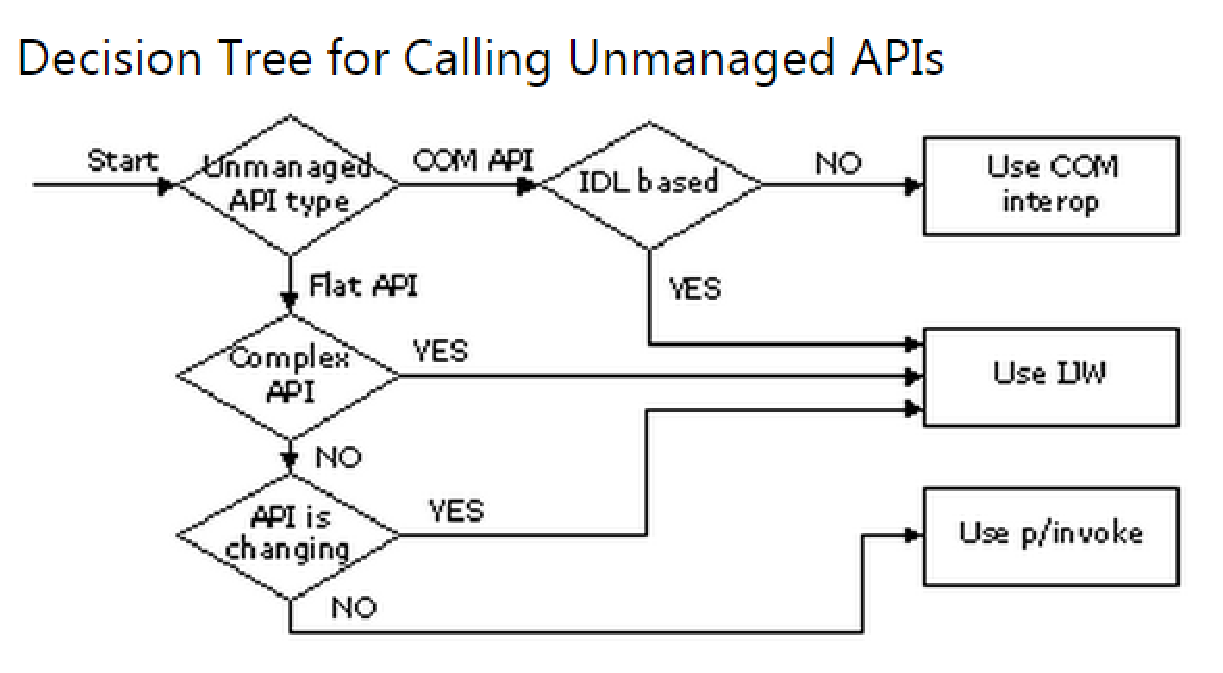
\includegraphics[height=6cm,
    angle=0]{./images/how2call_unmanagedAPI.eps}}
  \caption{Decesiion tree for calling unmanaged APIs}
  \label{fig:how2call_unmanagedAPI}
\end{figure}


Platform Invoke (P/Invoke) and COM (Component Object Model) interoperation
allows managed code to use native functionality.

P/Invoke provides the functionality to access functions, structs, and callbacks
in unmanaged DLLs. P/Invoke provides a translation layer to assist developers by
allowing them to extend the library of available functionality beyond the
managed library of the BCL. 

P/Invoke is a nice technology and it works fairly well, except for issues in
loading the target dll. We've found that the best way to do things is to create
a static library of native functions and link that into a Managed C++ (or
C++/CLI) project that depends upon it.  To call C++ code from C\#, one easy way
is to create a wrapper assembly in C++/CLI. In C++/CLI you can call into
unmanaged code as if you were writing native code, but you can call into C++/CLI
code from C\# as if it were written in C\#.

Example: Step 1 - C++/CLI
\begin{verbatim}
// compile: /CLR 
#include "NativeType.h"

public ref class ManagedType
{
     NativeType*   NativePtr; 

public:
     ManagedType() : NativePtr(new NativeType()) {}
     ~ManagedType() { delete NativePtr; }

     void ManagedMethod()
      { NativePtr->NativeMethod(); } 
}; 
\end{verbatim}

Example: Step 2 - in C\#
\begin{verbatim}
ManagedType mt = new ManagedType();
mt.ManagedMethod();
\end{verbatim}

Example: Step 1 - C++/CLI
\begin{verbatim}
#pragma managed(push, off)
#include "oldskool.h"
#pragma comment(lib, "oldskool.lib")
#pragma managed(pop)

using namespace System;

public ref class Wrapper {
private:
    COldSkool* pUnmanaged;
public:
    Wrapper() { pUnmanaged = new COldSkool; }
    ~Wrapper() { delete pUnmanaged; pUnmanaged = 0; }
    !Wrapper() { delete pUnmanaged; }
    void sampleMethod() { 
        if (!pUnmanaged) throw gcnew ObjectDisposedException("Wrapper");
        pUnmanaged->sampleMethod(); 
    }
};
\end{verbatim}

\subsection{Access COM APIs from managed code}


{\bf Suppose you have a COM and you want to use in .NET managed code}: 



There are only one way
\begin{enumerate}
  \item COM interop: available in all managed languages
\end{enumerate}
OLE Automation-compatible COM components. The CLR will take care of COM
component activation and parameter marshaling. 

COM interop relies on information from type libraries to make correct interop
calls, but type libraries typically do not contain all the information present
in IDL files. Using C++ interop solves this problem by allowing direct access to
these COM APIs.  

For companies that own COM APIs that have already shipped, it is important to
consider shipping primary interop assemblies (PIAs) for these APIs, thus making
them easy to consume for managed clients. 




\subsection{Access managed code from native code}


{\bf Suppose you have .NET managed code in assembly, and you want to use in C++ code}
\begin{itemize}
  \item write the C++/CLI code to mix the .NET managed code and C++ code (Sect.\ref{sec:C++/CLI}).
\end{itemize}


There are two main ways to expose a managed API to purely unmanaged callers
\begin{enumerate}
  \item as COM API via COM interop: enable call to COM APIs in any managed
  language from unmanaged code. COM interop is comprised of core services provided by the CLR,
  plus some tools and APIs in the System.Runtime.InteropServices namespace.
  
  Every public managed class can be exposed to unmanaged clients through COM
  interop. This process is easy to implement. Despite the fact that exposing
  managed APIs as COM APIs is easy, managed and COM object models are very
  different.
  Some features available in the managed world have no equivalent in the COM
  world and will not be usable from COM clients. Because of this, there is often
  tension between managed API design guidelines (DG) and compatibility with COM.
  
  Every managed class appears to implement IUnknown, IDispatch,
  ISupportErrorInfo, and a few other standard COM interfaces. 
  
  \item as a flat API (if the native code is C++)
  
  Sometimes unmanaged clients cannot use COM. For example, they might already be
  written to use flat APIs and cannot be changed or recompiled. C++ is the only
  high-level language that allows you to expose managed APIs as flat APIs. Doing
  this is not as straightforward as exposing a managed API as a COM API. It is a
  very advanced technique that requires advanced knowledge of C++ interop and
  the differences between the managed and unmanaged worlds.  
  
  \item (if the native code is C++ and we can recompile the C++ code into mixed
  mode image using VS.NET C++ compiler (i.e. C++/CLI compiler), then the
  unmanaged code can directly access any managed API) via C++ interop (sometimes referred to as It Just
  Works (IJW)) is a C++-specific feature, which enables flat APIs and COM APIs
  to be used directly, as they have always been used. This is more powerful than
  COM interop, but it requires much more care. Make sure that you check the C++
  resources before you use this technology.
  
  For C++ unmanaged clients that are willing to recompile their code with Visual
  Studio .NET, there is a third option: directly accessing managed
  functionality through C++ interop. Suggestions for how and when to use these
  options are described in this section.  
\end{enumerate}

C++/CLI programming language (See C/C++ manual book) let us write managed and
native code in the same program. First, compile the program with \verb!/clr!
switch, then the compiler create metadata for the application that can be
consumed by other managed asemblies, and enables the applications to consume
types and data in the metadata of other managed components.

\url{http://msdn.microsoft.com/en-us/library/ms717435(v=vs.100).aspx}


\subsection{Mixed code}

{\bf Suppose you want to write a program that accepts both native code and managed code}
\begin{itemize}	
  \item Managed C++ (Sect.\ref{sec:managed_C++}) 
  \item C++/CLI (Sect.\ref{sec:C++/CLI})
\end{itemize}


\section{.NET tools}
\label{sec:NET_tools}

.NET provde 3 new tools
\begin{enumerate}
  \item \verb!IntPtr!: a platform-dependent representation of a memory address
  \item \verb!GCHandle! :  can pin and retrieve the address of data in the
  managed memory heap
  \item \verb!Marshal! class: a one-stop portal for all memory operations, e.g.
  allocation, cleanup, and manipulaiton needs.
\end{enumerate}

In .NET 1.0 and 1.1, all operating system handles could be encapsulated only by
an \verb!IntPtr! object. However, this managed way to interact with unmanaged
resource is not safe.  IntPtr allowed handles to be leaked, particularly by
asynchronous exceptions. These exceptions present a huge hurdle for the garbage
collector (GC) being able to clean up those resources.  
To resolve such problems, .NET 2.0 then provides \verb!SafeHandle! and
\verb!ContrainedExecutionRegion! (CER) region. 
\url{http://www.codeproject.com/Articles/16157/SafeHandle-and-Constrained-Execution-Regions}



\section{IntPtr}
\label{sec:IntPtr}

\verb!IntPtr! is a structure to represent both addresses and handles (most
handles are pointers to Windows pointers). 
\begin{itemize}
  \item it is 32-bit on a 32-bit O/S
  \item it is 64-bit on a 64-bit O/S
\end{itemize}
Any function within the .NET Framework that exposes a way to work with addresses
and handles, uses the IntPtr type.

IMPORTANT: \verb!IntPtr! is similar to \verb!void *! in C/C++, i.e. a pointer
pointing to any object.

\section{SafeHandle vs. CriticalHandle vs. IntPtr}
\label{sec:SafeHandle}

\url{http://msdn.microsoft.com/en-us/library/ms182294.aspx}

\url{http://stackoverflow.com/questions/11973109/can-i-use-safehandle-instead-of-intptr}


\section{P/Invoke (.NET languages): Interop Marshalling}
\label{sec:marshalling}
\label{sec:P/Invoke}

.NET Framework 1.0 provides a way for managed code to call unmanaged functions
residing in DLLs, e.g. Win32 APIs.
P/Invoke: enable call any function in any unmanaged language as long as
  its signature is redeclared in managed source code. \textcolor{red}{If we just
  use a few flat APIs (or even complex flat APIs), then this is recommended to
  use.}
  
\begin{mdframed}
\textcolor{red}{complex flat API: APIs that have signatures that are hard to
declare in managed language. For example, methods with variable size structure parameters
are hard to declare since there is no equivalent concept in the managed type
system.}
\end{mdframed}
  
  
This include 3 primary steps in the managed
code
\begin{enumerate}
  \item declaration, i.e. define the interface of the unmanged code API (Sect.\ref{sec:P/Invoke_declaration}).
  
     At design time, we need to tell which unmanaged API you intend to call.
     This
includes (1) DLL name (i.e. the module), (2) function name (i.e. entry point),
(3) calling convention to use which includes Marshalling the data type so that
.NET understand the equivalent data type representation for parameter passing.
  
  \item invocation, i.e. calling the API via this interace
  
  
  \item error handling 
\end{enumerate}


\subsection{Declaration}
\label{sec:P/Invoke_declaration}

\subsubsection{Declaration: marshall functions}
\label{sec:marshall_API}

REQUIREMENT: The methods in the DLL need to be coded using 
\verb!__declspec(dllexport)! (Sect.\ref{sec:__declspec(dllexport)})
\begin{verbatim}
extern "C"  __declspec(dllexport) int MyMethod(int x)
{

}
\end{verbatim}

NOTE: We just provide the method declaration (ended with a semicolon) and it is
often use with \verb!DllImport! attribute.
\begin{itemize}
  \item we can put the API inside a class if we like
  

TIPS: It is suggested to put all APIs of a DLL inside the same class, within an
appropriate namespace. This class can be packaged in its own assembly and
distributed to all of the developers on your team or in your organization.
  
  \item alias can be used: the function name being used in the managed code can
  be different from the DLL's API. Then, \verb!EntryPoint! attribute need to be
  used to indicate the DLL's API name.
  
  
  \item another important thing is to use \verb!System.Runtime.InteropServices! in your
C\# code. The System.Runtime.InteropServices namespace provides a collection of
classes useful for accessing COM objects, and native APIs from .NET
  
  \item Final step, in order to build and run your C\# application, the DLL file must be
in the same folder of the C\# EXE file.
  
\end{itemize}
\begin{verbatim}
using System;
using System.Runtime.InteropServices;

class MyClass
{
  [DllImport("User32.dll")]
  public static extern Int32 MyMethod(Int32 x);
  
  
}

[DllImport("TestLib.dll")]

public static extern void DisplayHelloFromDLL ();

\end{verbatim}
The keyword \verb!extern! means that the method is implemented externally
(Sect.\ref{sec:keyword_extern}).


As \verb!Int32! is the equivalent .NET data type of C++ \verb!int! data type, there is no need for interop marshalling. The list of equivalent data type is given
\begin{verbatim}
C++ Type      .NET Framework Type           Blittable

bool           System.Boolean               N

signed char    System.SByte                 Y

unsigned char  System.Byte                  Y

wchar_t        System.Char                  N

double, long double
              System.Double                 Y

Float         System.Single                 Y

int, signed int, long, signed long
              System.Int32                  Y

unsigned int, unsigned long
              System.UInt32                 Y

__int64, signed __int64
             System.Int64                   Y

Unsigned __int64
             System.UInt64                  Y

short, signed short
             System.Int16                   Y

Unsigned short
             System.UInt16                 Y


\end{verbatim}
\url{http://www.codeproject.com/Articles/16987/C-Interop-is-for-the-Performance-Minded-Developer}

% In the C\# project, if we want to use the DLL above, in one source file, we add
% (suppose the DLL name is TestLib.dll, and the function we want to use from the
% DLL is DisplayHelloFromDLL())
% \begin{verbatim}
% \end{verbatim}

Example: define an alias
\begin{verbatim}
[DllImport("coredll.dll", EntryPoint="SHGetSpecialFolderPath")]
static extern bool GetFolderPath( //the rest of the declaration
\end{verbatim}
You can also define an alias of the function to use in managed code, and the
original name in unmanaged API should be given as the value of \verb!EntryPoint!
inside \verb!DllImport! attribute.


Example:
\begin{verbatim}
using System;
using System.Runtime.InteropServices;     // DLL support

class HelloWorld
{
    [DllImport("TestLib.dll")]
    public static extern void DisplayHelloFromDLL ();

    static void Main ()
    {
        Console.WriteLine ("This is C# program");
        DisplayHelloFromDLL ();
    }
}
\end{verbatim}

%\subsection{In the original DLL code}

Example:
\begin{verbatim}
[DllImport("coredll.dll", SetLastError=true)]
private static extern bool SHGetSpecialFolderPath(
   int hwndOwner, 
   string lpszPath,
   ceFolders nFolder,
   bool fCreate);
\end{verbatim} 
The function \verb!SHGetSpecialFolderPath! is marked as private as we only want
it to be called inside the class in which it is declared. Using \verb!extern!
modifier is required to indicate that the function is implemented externally
and using \verb!static! means the method can be called without creating an
instance of the class. The data type we use here must be the equivalent type
mentioned in Sect.\ref{sec:marshal_types}.
\url{http://msdn.microsoft.com/en-us/library/aa446536.aspx}

\begin{mdframed}
NOTE: coredll.dll is the Windows CE APIs equivalent to Win32 API filename: 
kernel32.dll, user32.dll.
\end{mdframed}




% \subsection{Expose function name inside a class}
% 
% At first, we need to wrap these unmanaged methods inside a class, i.e. declare
% the unmanaged function as a method of this class. To do so, we use \verb!DllImport! attribute which
% contains the DLL filename, then come the interface of the funciton using
% \verb!static extern! modifier.



\subsubsection{Declaration: marshall data types}
\label{sec:marshal_types}

During the invocation process (Sect.\ref{sec:invoke_wrapper-methods}), the
P/Invoke service is responsible for marshalling parameter values passed to the
DLL function. This is done by the component called {\bf marshaller} in the
P/Invoke service. 

There are two cases of data types: {\bf blittable types}
(Sect.\ref{sec:marshall_blittable-types}) and non-blittable data types.

\subsection{Passing blitable types}
\label{sec:marshall_blittable-types}

If the data type has the same representation between managed code and unmanaged
code, we call them {\bf blittable types} then the marshaller does not have to do
any special handdling to convert the data so that it is interpreted correctly by
the unmanaged code (i.e. marshalling process for the arguments) and
the managed code (i.e. unmarshalling process for the returned value). If the one
dimensional array of these blittable types, or even structure or classes that
contains only these types (except \verb!System.String!), the marshaller does not
have to do anything.

and we can use the right keyword
\begin{verbatim}
 System                     C# keyword-to-use        C/C++
System.Byte                   byte                   int
System.SByte                  sbyte
System.Int16                  short
System.UInt16                 ushort
System.Int32                  int
System.Int64                  long
System.UInt64                 ulong
System.IntPtr                 *   (using 'unsafe' keyword)


    (additional to .NET Compact Framework)
System.Char                    char
System.String                  string
System.Boolean                 bool
    
\end{verbatim}
As .NET Compact Framework only support Unicode, the  marshaler always marshals
System.Char as a 2-byte Unicode char and System.String as a Unicode
null-terminated array. Also, System.Boolean is marshalled as 1-byte integer
value; whereas .NET Framework use 4-byte integer value. 

At the time of invocation, \verb!System.String! is a reference type (it is
allocated in the managed heap, and the address is stored in the reference
variable), even though it is passed by value, the marshaller still passes a
pointer to the string to the unmanaged function.

IMPORTANT: .NET Compact Framework always passes a pointer to a reference type,
and does not support passing reference type by reference (i.e. using \verb!ref!
keyword in C\#), which makes the unmanaged code to see the string as one of the
following type
\begin{verbatim}
WCHAR*
TCHAR*
LPTSTR
LPSTR
\end{verbatim}
and manipulate the string using pointer (\textcolor{red}{This is different
from .NET Framework}). Nevertheless, when the function completes, the caller can
inspect the string as normal. 

In .NET Framework, the marshaler must take the character set into consideration.
As a result, the full .NET Framework does not support passing strings by value
or by reference into unmanaged functions and allowing the unmanaged function to
modify the contents of the buffer. Instead, we need to wrap the string into a
\verb!System.Text.StringBuilder! object and pass this object by pointer to the
unmanaged code. The only caveat is that if we decide to modify the content, the
object must be pre-allocated with enough space for the return value, or the text
will overflow, causing an exception thrown by P/Invoke service.

\begin{verbatim}
[DllImport("coredll.dll", SetLastError=true)]
private static extern bool SHGetSpecialFolderPath(
   int hwndOwner, 
   StringBuilder lpszPath,
   ceFolders nFolder,
   bool fCreate);


.............

Dim sPath As New StringBuilder(MAX_PATH)
ret = SHGetSpecialFolderPath(0, sPath, folder, False)
\end{verbatim}
 
IMPORTANT: Although System.String is a blittable type in the .NET Compact
Framework, it is not blittable when used inside a complex object, such as a
structure or class.

\subsection{Passing objects of structure or class type}

If the structure or class only contains data members of blittable types
(Sect.\ref{sec:marshall_blittable-types}), then you can pass directly the
structure or class type without worrying. The choose between struct and class is
that object of type struct is passed by value; while object of class type is
passed by reference. With pass by reference, marshaller always use a 4-byte
pointer to the reference type in the unmanaged code. Also, the layout of the
data members in the structure and the class is in the order in which they appear
in the managed code. However, to have a control on the layout, we can 
decorate the structure with \verb!StructLayout! attribute and
\verb!LayoutKind.Sequential! 

Example: when we define the wrapper method
\begin{verbatim}
// VB.NET
Private Structure MEMORY_STATUS
  Public dwLength As UInt32
  Public dwMemoryLoad As UInt32
  Public dwTotalPhys As UInt32
  Public dwAvailPhys As Integer
  Public dwTotalPageFile As UInt32
  Public dwAvailPageFile As UInt32
  Public dwTotalVirtual As UInt32
  Public dwAvailVirtual As UInt32
End Structure

<DllImport("coredll.dll", SetLastError:=True)> _
Private Shared Sub GlobalMemoryStatus(ByRef ms As MEMORY_STATUS)
End Sub
\end{verbatim}

\begin{mdframed}
In .NET Compact Framework, the marshaller cannot marshall complex objects
(reference types) within structures. This means that if the structure contain a
member of a type not of blittable types, the structure cannot be fully
marshalled. 
\end{mdframed}

To marshall a complex object in .NET Framework, we use \verb!MarshallAs!
attribute, to explicitly tell the marshaller how to marshall the data members. 

\subsection{Invoke the wrapped method}
\label{sec:invoke_wrapper-methods}

After you define the class with the methods marshalling the unmanaged APIs
(Sect.\ref{sec:marshall_API}) and the equivalent data types
(Sect.\ref{sec:marshal_types}), we can compile the class into an assembly, and
use it as a regular managed code inside another managed code.

As the wrapper method can raises an error, whenever we call it, we need to wrap
inside a \verb!try/catch! block (Sect.\ref{sec:marshall_handling-errors}
describes potential exceptions)
\begin{verbatim}

public string MyFunctionUseUnmanagedFunction()
{ 
   try{
     ret = SHGetSpecialFolderPath(0, sPath, folder, False);
   }
   catch (ex As Exception)
   {
        HandleCeError(ex, "GetSpecialFolderPath");
        Return Nothing;
   }   
   if (!ret)
   {
    // API error and retrieve error number
    int errNum = Marshal.GetLastWin32Error();
   }
   
   return sPath;
}      
\end{verbatim}

At runtime, the code is JIT compiled at runtime and the P/Invoke service of the
CLR extracts the \verb!DllImport! definition from the metadata of the assembly,
locate and load the DLL containing the function into memory, and then retrieve
the address of the function using the entry point information.
If all goes well, the function will then be invoked, its arguments marshaled,
and any return values passed back to the caller.

\subsection{Handling errors}
\label{sec:marshall_handling-errors}


Although developers never expect their code to generate runtime errors, it is
important to remember that functions invoked on DLLs using P/Invoke can generate
two different kinds of errors.
\begin{enumerate}
  \item \verb!NotSupportedException! is raised: exception generated by the
  P/Invoke service itself, i.e. when the arguments passed to the method
  contains invalid data, or the function is declared with incompatible interface with the entrypoint's function in
  unmanaged DLL.
  
  \item \verb!MissingMethodException! is raised: P/Invoke service throw this
  exception if the entrypoint is not found in the unmanaged DLL.
\end{enumerate}


\subsection{TIPS: string encoding}


\section{Using pointers: unsafe code}

In CLR,  unsafe code is referred to as unverifiable code.Unsafe code in C\# is
not necessarily dangerous; it is simply code whose safety cannot be verified by
the CLR. Also, remember that  unsafe code cannot be executed in an untrusted environment.
For example, you cannot run unsafe code directly from the Internet.


Using pointers in C\# is recommended in scenarios
\begin{enumerate}
  \item performance-critical code
  
Example: In situations where you are doing extremely intensive operations
against large blobs in memory, for example image manipulation, it is faster to
step outside the normal safety the runtime provides.


  \item advanced COM or P/Invoke scenarios that involves structures with pointer
  in them.
  \item dealing with existing structures on disk
\end{enumerate}

There, we need to put the code inside \verb!unsafe! context to allow pointers.

\section{C++ interop (Visual C++): dllexport, dllimport}
\label{sec:interop_C_Csharp}

Since Visual Studio 2005, Visual C++ (under the name C++/CLI -
Sect.\ref{sec:C++/CLI} of C/C++ manual book) supports interoparability that
enables both managed code and unmanaged code to exist in the same application,
and even in the same file (using \verb!#managed!, \verb!#unmanaged! pragmas).
Visual C++ supports the creation of three distinct types of components and
applications: mixed, pure, and verifiable. All three are available through the
\verb!/clr! (Common Language Runtime Compilation) compiler option.

C++ interop (available in C++): it requires to introduce a whole new
  module written in C++. So use this if the unmanaged flat APIs are changing
  while managed code is under development. The C++ layer can be very thin and
  the rest of the managed code can be written in any other managed language of
  choice. Using C++ interop solves this problem by allowing direct access to
  unmanaged APIs - which requires no rewriting, just the inclusion of a header
  file. 

This allows Visual C++ to integrate .NET functionality into existing Visual C++
applications without disturbing the rest of application. 

C++ Interop is better than P/Invoke (Sect.\ref{sec:P/Invoke}) if the interface
of the functions from DLL keeps changing. It also provides better type safety,
and make performance enhancements possible that are not possible with P/Invoke.
C++ Interop uses the fastest possible method of data marshaling, whereas
P/Invoke uses the most robust method. This means that C++ Interop (in a fashion
typical for C++) provides optimal performance by default, and the programmer is
responsible for addressing cases where this behavior is not safe or appropriate.  
 
However, C++ Interop is not possible if the unmanaged source code is not
available or when compiling with /clr:safe

% \section{C++ COM Interop}
% 

% 
% 
% \section{C++ code call managed classes directly}
% 
% 
% There are two options
% \begin{enumerate}
%   \item make the C++ code become C++/CLI code, by compiling with \verb!/clr! options
%   
%   \item wrap the managed classes in a DLL with native entry points
% \end{enumerate}

\section{/clr option}
\label{sec:clr_option}

The \verb!/clr! option is used to compile mixed code (managed + native) -
Sect.\ref{sec:managed_C++} and Sect.\ref{sec:C++/CLI}.
There are different options, Fig.\ref{fig:clr_option}.
\url{https://msdn.microsoft.com/en-us/library/k8d11d4s.aspx}

\begin{figure}[hbt]
  \centerline{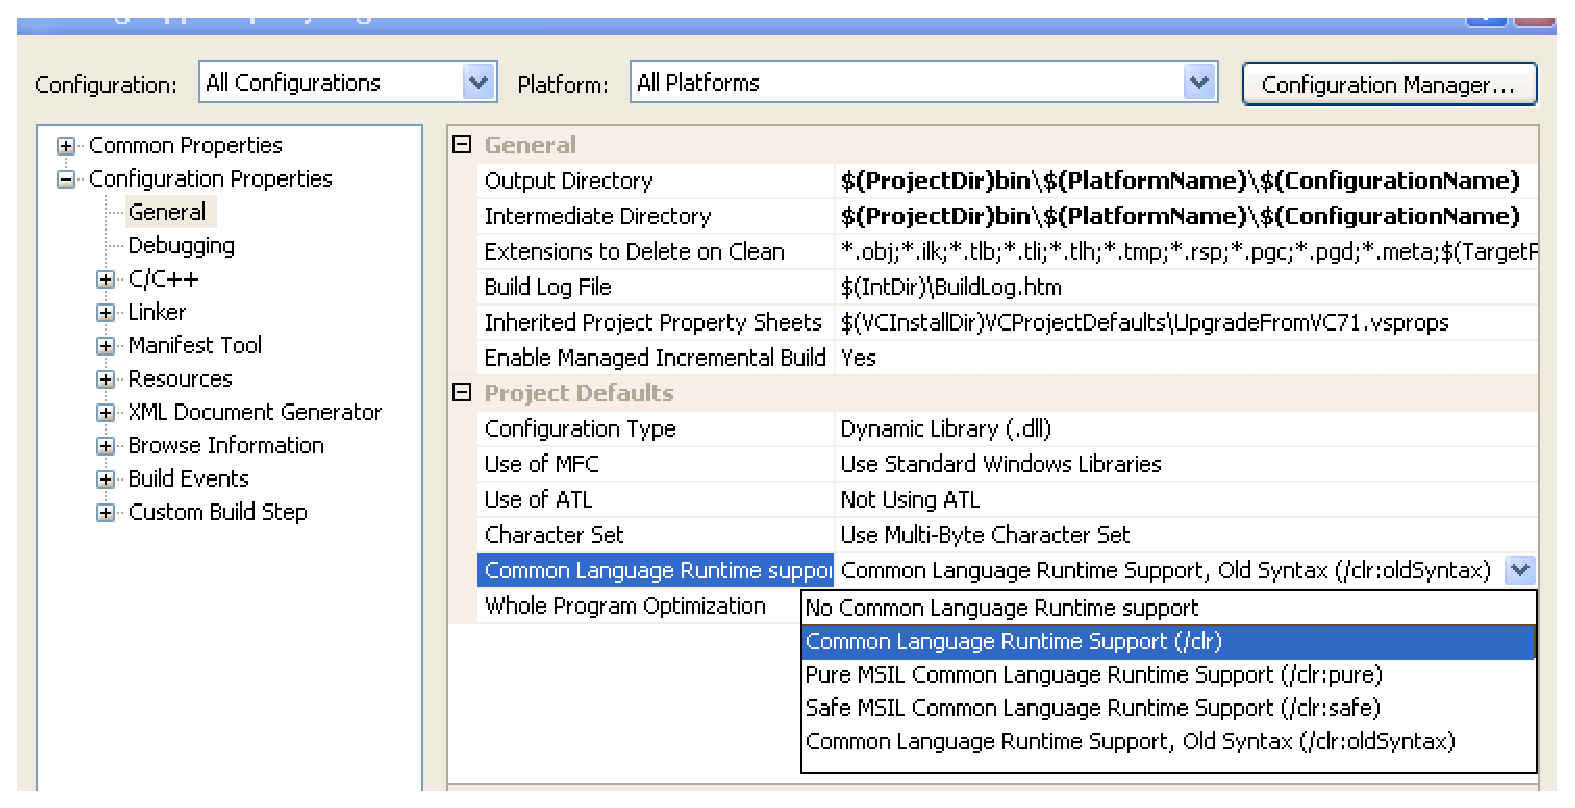
\includegraphics[height=2.7cm,
    angle=0]{./images/clr_option.eps}}
\caption{/clr options}
\label{fig:clr_option}
\end{figure}


\begin{verbatim}
Project properties
   Configuration Properties
      General
\end{verbatim}
There are a few options:
\begin{enumerate}
  \item No Common Language Runtime Support: compile your code as native code

  \item Common Language Runtime Support, Old syntax (/clr:oldSyntax) : compile Managed C++ code (Sect.\ref{sec:managed_C++}) in Visual Studio 2008 and above. 
  
  This can be removed anytime in the future.
  
  \item Common Language Runtime Support (/clr): compile C++/CLI code
  
  \item Pure MSIL Common Language Runtime Support (/clr:pure): Produces a Microsoft Intermediate Language (MSIL)-only output file that has no native executable code. However, it can contain native types compiled to MSIL. 
  
  \item Safe MSIL Common Language Runtime Support (/clr:pure): Produces an MSIL-only (no native executable code)
  
\end{enumerate}

\url{http://stackoverflow.com/questions/4094832/converting-from-c-cli-oldsyntax-how-to-and-can-this-be-automated}

The mixed code can be an executable file, or a library. 
\begin{itemize}
  \item To enable debugging: add \verb!/ASSEMBLYDEBUG! 
  \url{https://msdn.microsoft.com/en-us/library/cta4x5hc.aspx}
  
  \item Use \verb!#pragma unmanaged! to specify the region of code to be compiled to native code.
  and use \verb!#pragma managed! to switch back to managed code region.
   
  \item Code must be compiled with \verb!/MD!, which ensure 
  the dynamically linked, multithreaded versions of the runtime routines are selected from the standard header. 
  This is a known limitation as the CLR garbage collector runs finalizers on a different thread.
   
\end{itemize}
\url{https://msdn.microsoft.com/en-us/library/k8d11d4s.aspx}

\section{Troubleshoot}


In VS 2008 (Sect.\ref{sec:VS_2008}),  the 32-bit mixed code can give an
exception about some code that was not created on the managed heap, when
something calls \verb!CrtIsValidHeapPointer()!. A solution was
adding 
\begin{verbatim}
__DllMainCRTStartup@12
\end{verbatim}
to 
\begin{verbatim}
Project properties
   Linker 
     Input
        Force Symbol References
         __DllMainCRTStartup%4012;%(ForceSymbolReferences)
\end{verbatim}

However, in 64-bit application, this gives an error
\begin{verbatim}
Linking...
1>LINK : error LNK2001: unresolved external symbol __DllMainCRTStartup@12
-------------------
\end{verbatim}
A solution for 64-bit application is adding
\begin{verbatim}
_DllMainCRTStartup

// or

_DllMainCRTStartup;%(ForceSymbolReferences) 
\end{verbatim}
(one underscore, no "@12" postfix) as the exported functions are not decorated
\url{https://social.msdn.microsoft.com/Forums/en-US/bf162181-864c-4c25-88b0-b56d1affe350/crtisvalidheappointer-vs-dllmaincrtstartup12-in-vs2008-x64?forum=netfx64bit}
\import*{../Fortran_Manual/}{FortranCpp.tex}
\chapter{Swig}

SWIG is a compiler that makes it easier to integrate C/C++ code with
many other languages (Perl, PHP, Tcl, Ruby, Python, Java, OCaml, C\#, \ldots).

Swig takes a set of ANSI C/C++ declarations and generates the
equivalent interfaces in other languages. 

\begin{verbatim}
sudo apt-get install swig
\end{verbatim}

\chapter{Vala programming language}
\label{chap:vala-language}


\section{vala programming language: valac compiler}
\label{sec:valac}
\label{sec:vala-language}

Vala is a new object-oriented programming language, that translate vala source
code into C source and header files. It uses GObject type system to create classes and
interfaces (Sect.\ref{sec:GObject}).

Vala aims to bring modern programming language features to GNOME developers
without imposing any additional runtime requirements and without using a
different ABI compared to applications and libraries written in C.

Ubuntu 14.04 only has valac 0.22; if you needs newer version, follow the steps
\begin{verbatim}
sudo add-apt-repository ppa:ricotz/testing 
sudo apt-get update
sudo apt-get install valac
\end{verbatim}
\url{https://askubuntu.com/questions/612342/how-to-install-the-vala-environemt}

Vala is syntactically similar to \verb!C#! and includes several features such
as:
anonymous functions, signals, properties, Ggenerics, assisted memory management,
exception handling, type inference, and foreach statements 


\section{GObject}
\label{sec:GObject}

GObject is used by vala language (Sect.\ref{sec:vala-language})

If we need GObject introspection, we need to install
\begin{verbatim}
sudo apt-get install gobject-introspection  -y
  // the below package also include
  // gobject-introspection1.0-dev 
  //  handling GObject introspection data (development files)
sudo apt-get install libgirepository1.0-dev -y 
\end{verbatim}

\part{Extras}
\chapter{Interview Questions}


\section{Encapsulation vs. Polymorphism}
\label{sec:encapsulation}
\label{sec:polymorphism}

Encapsulation is a mechanism of a programming language to limit the access from
one class to another. In C++, there are three level of encapsulation: private,
public and protected:
\begin{enumerate}
  \item protected: only the current class and its subclass can have access to
  its field data and methods.
  \item public: the field data or method can be access from outside  
  \item private: only the current class can access to its field data or method
\end{enumerate}


Polymorphism refers to the programming language's ability to process objects
differently depending on their data type/class it is pointing to. It ties
closely with the concept {\it inheritance}. Polymorphism is NOT the same as
method overloading (i.e. methods same name but different output interface) or
method overriding (i.e. rewrite the content).


\section{Compile-time polymorphism vs. Run-time polymorphism}


\subsection{runtime polymorphism (dynamic polymorphism)}
\label{sec:polymorphism-runtime}
\label{sec:runtime-polymorphism}

{\bf It's about subclassing (and method overriding)}: It's being used in
pointer, i.e. reference of class X can hold object of class X or an object of
any sub classes of class X.
\begin{verbatim}
X obj = new Y(); // class Y:: X {}

X obj = new X();
\end{verbatim}

If the derived class Y has override the method defined in X, so at runtime, the
compiler need to know whether \verb!obj! is pointing to X or Y to call the right
method. This is known as runtime polymorphism.

\subsection{compile-time polymorphism (static polymorphism)}
\label{sec:polymorphism-static}
\label{sec:compile-time-polymorphism}

{\bf It's about method overloading} (C++, Java)
A class can have more than one methods with same name but with different number
of arguments or different types of arguments or both. 
It may or may not have same return type. IMPORTANT: We cannot overload just by
return type, i.e. at least one parameter must be different. This behavior is
same in Java and C++.

When the compiler scanning through the code for compiling, the compiler is able
to figure out the exact method call at compile-time that's the reason it is
known as compile time polymorphism.

In C++, templating is a case of method overloading
(Sect.\ref{sec:template-C++98}), i.e. different types can be used in a function
to represent the same concept, despite being completely unrelated.
\begin{lstlisting}
template <typename T>
T add(const T& lhs, const T& rhs) { return lhs + rhs; }
\end{lstlisting}
Here, there is no need for subclassing, except the type T just has to define
the + operator. 

\begin{mdframed}
Templates as in C++ do not exist in Java. The best approximation is generics.
\url{http://stackoverflow.com/questions/2159338/what-is-the-java-equivalent-of-cs-templates}
\end{mdframed}

\url{http://stackoverflow.com/questions/2128838/compile-time-polymorphism-and-runtime-polymorphism}

\section{Code execute only once}

Suppose that you have a function that get call multiple times, yet there is once
piece of code in that function that you want to be run only once.

\subsection{pthread\_once\_t (Linux only)}

Use \verb!pthread_once_t!, and make the function/method that you want to call
once a \verb!static! function/method.

\begin{lstlisting}
#include <pthread.h>

//1. define a variable as static 
static pthread_once_t semaphore = PTHREAD_ONCE_INIT;

class FooBar()
{
 public:
   static void test(); //must be static and void
   int somefunction();
}

//2. map that variable to the function to be called once
void FooBar::test()
{ // code to run once
}
int FooBar::somefunction()
{
   pthread_once( & semaphore, FooBar::test() );
   
   // do others
   ...
}
\end{lstlisting}
\url{http://stackoverflow.com/questions/6911126/is-it-possible-to-define-the-static-member-function-of-a-class-in-cpp-file-inst}

\url{http://apiexamples.com/c/pthread/pthread_once.html#L0}
\url{https://www-01.ibm.com/support/knowledgecenter/ssw_aix_71/com.ibm.aix.basetrf1/PTHREAD_ONCE_INIT.htm}


\subsection{boost::call\_once, boost::once\_flag (portable, thread-safe)}
\label{sec:boost::call_once}

We use \verb!boost::call_once!.
This has become part of C++11 (Sect.\ref{sec:std::call_once-C++11})


\begin{lstlisting}
    static boost::once_flag flag = BOOST_ONCE_INIT;
    boost::call_once([]{callee();}, flag);  
\end{lstlisting}
The first line can be inside or outside a function, since it is static.

\subsection{Define a static class}

Suppose the function you want to call once is \verb!callee()!, to be called by 
the function \verb!caller()!. The treat is define a static class object; with
the constructor calls \verb!callee()!.

IMPORTANT: This is not thread-safe in C++03, thread-safe in C++0x. 

\begin{verbatim}
void caller()
{
    static class Once { public: Once(){callee();}} Once_;
}
\end{verbatim}
\url{http://stackoverflow.com/questions/4173384/how-to-make-sure-a-function-is-only-called-once}

\subsection{std::call\_once, std::once\_flag (C++11)}
\label{sec:std::call_once-C++11}


\begin{verbatim}
template< class Callable, class... Args >
void call_once( std::once_flag& flag, Callable&& f, Args&&... args );
\end{verbatim}
The Callable $f$ is called only once, even if called from several threads.

We need to pass an object of \verb!std::once_flag! along with the function to be
called $f$ to \verb!call_once()!. Any call to $f$ with the same
\verb!std::once_flag! object ensures $f$ only run 1 time.

\begin{lstlisting}
#include <thread>
#include <mutex>

std::once_flag flag1, flag2;

void may_throw_function(bool do_throw)
{
}

void do_once(bool do_throw)
{
  try {
  // do_throw is the argument of may_throw_function
    std::call_once(flag2, may_throw_function, do_throw);
  }
  catch (...) {
  }
}

\end{lstlisting}
\url{http://en.cppreference.com/w/cpp/thread/call_once}

\subsection{constructor attribute GCC}

constructor function \verb!__attribute__! of GCC

\url{http://stackoverflow.com/questions/8412630/how-to-execute-a-piece-of-code-only-once}

\section{Write a function that dynamically allocate a 2D array and return it
back to the caller}

\begin{lstlisting}
int ** pdata; // a 2D array [X][Y]

void createData(pdata, int &X, int &Y); 

// free memory
for(int i = 0; i < X; ++i) {
    delete [] ary[i];
}
delete [] ary;

\end{lstlisting}

NOTE: We can pass by reference
\begin{verbatim}
void createData(int** &pdata, int &x, int &y)
{
 // do some calculation to find 'x' and 'y'
 
 // allocate memory
 // Option 1:
 pdata = new int*[x];
 for(int i = 0; i < X; ++i) {
    pdata[i] = new int[Y];
 }
 // Option 2:
 pdata = (int**) malloc(sizeof(int*) * (X));
}

\end{verbatim}
 
\chapter{Project structure}

\section{Folder structure}

We should use one version manager, e.g. SVN. In one project, we should have the
following folders
\begin{verbatim}
branches
tools
trunk
vendor 
\end{verbatim}
and one file \verb!00README.TXT! to contains disclaiming information.
\begin{enumerate} 
  \item \verb!branches! should contain side-line development, experimental,
  development lines of multiple version of the same products (before putting in
  the stable release in \verb!trunk!.
  \item \verb!trunk! should contains only the main line of development
  \item \verb!vendor! to contain third-party libraries. When installing we
  should use the PREFIX=../../trunk/base.
\end{enumerate}


\subsection{trunk}

We should have the following folders
\begin{verbatim}
base
bin
doc
src
test
timing
verification
\end{verbatim}
where
\begin{itemize}
  \item \verb!base!: contains the folders of third-party libraries
  \item \verb!bin!: binary files
  \item \verb!doc!: documents (example or code manuals)
  \item \verb!test!: some test cases
  \item \verb!timing!:
  \item \verb!verification!: 
\end{itemize}

\subsection{src}

In the \verb!src! folder, we should have the following folders
\begin{verbatim}
arch
	- linux_laptop.mk
	- osx.mk
	- ...	
\end{verbatim}
and any other codes subfolders (to be discribed later). Important files
\begin{verbatim}
Makefile
Makefile.arch
\end{verbatim}
and other source codes files.

\subsection{Makefile}
\label{sec:Makefile_EP_EM}


We realize that using system name would help better select the proper setting,
rather using information about system architecture of 'uname' or any other
utilities. That's why we define the \verb!arc! folder, with files describing the
compiling configuration using the system name. The \verb!arch! should contains
different configuration setting for different system, e.g.
\verb!./arch/linux_laptop.mk! for the system \verb!LINUX_LAPTOP!. To know which
file is selected, \verb!Makefile! should include the file \verb!Makefile.arch!
first

Example: This is for EM
\begin{verbatim}
CXX=mpic++
CC=mpicc
LD=$(CXX)

#flags for defining macros
DFLAGS += -DWITH_MPI -DADD_ -D$(PLAT) -DUSE_CSTDIO_LFS

#base directory where to look for other third-party packages
BASE_DIR = $(PWD)/../base
# third-party packages
OOMPH_DIR = $(BASE_DIR)/oomph
SCOTCH_DIR = $(BASE_DIR)/scotch

##################
# Installation specific information
##################
# Flags for C pre-processor
EM_CPPFLAG = -DCARDIAC_BOOST -DCARDIAC_OPENMP -DWITH_MPI
AM_CPPFLAG = -DHAVE_CONFIG_H -I. -I$(OOMPH_DIR) -DOOMPH_HAS_MPI \
         -DOOMPH_HAS_TRIANGLE_LIB -DOOMPH_HAS_TETGEN_LIB \
         -DUSING_OOMPH_SUPERLU -DUSING_OOMPH_SUPERLU_DIST \
         -I$(OOMPH_DIR)/build/include -I$(SCOTCH_DIR)/build/include \
         -DLINUX_LAPTOP -I../base $(EM_CPPFLAGS)
         
# The solver is coded based on omph-lib         
# Include files and libraries for third_party
OOMPH-LIB_INCLUDE_DIR=$(OOMPH_DIR)/build/include
OOMPH-LIB_LIB_DIR=$(OOMPH_DIR)/build/lib
OOMPH-LIB_EXTERNAL_LIBS= -lHYPRE -lptscotch -lptscotcherr -loomph_hsl \
	-loomph_arpack -loomph_triangle -loomph_tetgen -loomph_superlu_3.0
	-loomph_parmetis_3.1.1 -loomph_superlu_dist_2.3 \
	-loomph_metis_from_parmetis_3.1.1 -lblas -llapack

EXTERNAL_DIST_LIBRARIES=-L$(BASE_DIR)/hypre/build/lib \
 	-L$(BASE_DIR)/scotch/build/lib
EXTERNAL_DIST_INCLUDE_DIR=$(BASE_DIR)/hypre/build/include

#Additional machine specific linking information that
# allows mixed-language compilation/linking
# e.g. Here is for RedHat Linux
FLIBS=-L/usr/lib/gcc/x86_64-redhat-linux/4.4.6 \
	-L/usr/lib64 -L/usr/lib/ -L/lib/ -L/lib64 \
	-lm -lgcc_s -L/reader_files
	
# Flags required for the shared libraries
SHARED_LIBRARY_PATH=-Wl, --rpath -Wl,$(OOMPH_DIR)/build/lib

CXXFLAGS_OPT = -g2 -O2 $(AM_CPPFLAGS) -I$(OOMPH-LIB_INCLUDE_DIR) \
	-I(EXTERNAL_DIST_INCLUDE_DIR)
CXXFLAGS_DEBUG = -g -O0 $(AM_CPPFLAGS) -I$(OOMPH-LIB_INCLUDE_DIR) \
	-I(EXTERNAL_DIST_INCLUDE_DIR)
\end{verbatim}
Depending on which system, we may need different APIs; what's why we need to
define a macro using the name of the system, e.g. \verb!LINUX_LAPTOP!. So, in
the code, if the API has different version, and to choose which one depending
on the system, we use 
\begin{verbatim}
#ifdef LINUX_LAPTOP
    call this_API
#else 
    call that_API
#endif
\end{verbatim}

The \verb!Makefile.arch! tells us the information about the \verb!ARCHGUESS!
macro, which is the name of the \verb!mk! file in the \verb!./arch! folder.
\begin{verbatim}
## Makefile.arch

#guess hostname with hostname command, stripping off all numbers
HOSTNAME := $(shell hostname -s | sed 's/[0-9]*//g')

#depending on the hostname, we define ARCHGUESS
ifeq ($(HOSTNAME), thunder)
  ARCHGUESS = thunder
endif
ifeq ($HOSTNAME), titan)
  ARCHGUESS = titan
 endif
 
# or we just simply override it
ARCHGUESS = linux_laptop

#Finally, if no result
ifndef ARCHGUESS
	$(error Unrecognized build host. Edit Makefile.arch)
endif
\end{verbatim}
the value of \verb!ARCHGUESS! will be used in \verb!Makefile! file as
\verb!ARCH! macro.

So \verb!Makefile! file
\begin{verbatim}
# Get name of architecture-specific incldue file 
SHELL = /bin/bash

# Define what are target-command
.PHONY: DEFAULT COMMON_TARGETS makedirs clean distclean depend

include Makefile.arch

ARCH ?= $(ARCHGUESS)

include arch/$(ARCH).mk

#keep version number of SVN
SVNVERSION := $(shell svnversion ./ )

#where to save binary (compiled file)
BINDIR = ../bin

HEARTSRC = \
	Cardioid.cc \
	... \  [here we list all source files]
	... \  [.cc = C++ source]

SPISRC= spi_impl.c
SIMDSRC= clooper.c TT06GatesSimd.c TT06Gates.c TT06NonGates.c \
	TT06NonGatesSimd.c workBound.c svd.c

DDCMD_FILES = \
	codata.h \
	ddcMalloc.c \
	ddcMalloc.h \
	... \
	...
	
DDCMDSRC = $(filter %.c, $(DDCMD_FILES))

HEARTOBJS = $(HEARTSRC:%.cc=$(OBJDIR)
\end{verbatim}


\verb!objs-$ARCH_FILENAME!

Example: This is for EP
{\small \begin{verbatim}
# Get name of architecture-specific include file from hostname
SHELL = /bin/bash

.PHONY: DEFAULT COMMON_TARGETS makedirs clean distclean depend

include Makefile.arch
# If defined, use architecture file set with ARCH variable
ARCH ?= $(ARCHGUESS)
include arch/$(ARCH).mk
\end{verbatim}}
which needs to read the compiling options from the architecture file, e.g. in
the case of system called \verb!peloton! with Intel microprocesors, we use
\verb!arch/peloton.mk!
\begin{verbatim}

CXX=mpic++ -fopenmp
CC=mpicc --std=gnu99 
LD=$(CXX)

DFLAGS = -DPELOTON -DWITH_PIO -DWITH_MPI \
    -DADD_ -DUSE_CSTDIO_LFS -D_LARGEFILE_SOURCE -D_FILE_OFFSET_BITS=64

INCLUDE =

CFLAGS_BASE = $(INCLUDE) $(DFLAGS)
CXXFLAGS_BASE = $(INCLUDE) $(DFLAGS)


CFLAGS_OPT =   $(CFLAGS_BASE) -g -O3
CFLAGS_DEBUG = $(CFLAGS_BASE) -g -ggdb -O0 -fno-inline
CFLAGS_PROF =  $(CFLAGS_BASE) -g -pg -O3 -DPROFILE

CXXFLAGS_OPT =   $(CXXFLAGS_BASE) -g -O3
CXXFLAGS_DEBUG = $(CXXFLAGS_BASE) -g -ggdb -O0 -fno-inline
CXXFLAGS_PROF =  $(CXXFLAGS_BASE) -g -pg -O3 -DPROFILE

LDFLAGS_OPT   = $(LDFLAGS_BASE) $(CFLAGS_OPT) $(CXXFLAGS_OPT)
LDFLAGS_DEBUG = $(LDFLAGS_BASE) $(CFLAGS_DEBUG) $(CXXFLAGS_DEBUG)
LDFLAGS_PROF  = $(LDFLAGS_BASE) $(CFLAGS_PROF) $(CXXFLAGS_PROF)
\end{verbatim} 

Now, the next content in the Makefile
 {\small \begin{verbatim}
SVNVERSION := $(shell svnversion ./ )

#------------------------------------------------------------------------------
#

BINDIR = ../bin

#NO main file is put here
HEARTSRC= \
    ThreadServer.cc \
    ThreadUtils.cc \
    stringUtils.cc \
    readCellList.cc \
    PioHeaderData.cc \
    ...

SPISRC=  spi_impl.c
SIMDSRC=  clooper.c TT06GatesSimd.c TT06Gates.c TT06NonGates.c TT06NonGatesSimd.c workBound.c svd.c

DDCMD_FILES = \
    codata.h \
    ddcMalloc.c \
    ddcMalloc.h \
    ddcMath.h \
    error.c \
    error.h \
    external.h \
    ...
DDCMDSRC = $(filter %.c, $(DDCMD_FILES)

\end{verbatim} }
All the source files of EP is \verb!HEARTSRC! macro, except the main file
(cardioid.cc). Now we add the main file
\begin{verbatim}
HEARTOBJS = $(HEARTSRC:%.cc=$(OBJDIR)/%.o)
HEARTOBJS += $(DDCMDSRC:%.c=$(OBJDIR)/%.o)
HEARTOBJS += $(SPISRC:%.c=$(OBJDIR)/%.o)
HEARTOBJS += $(SIMDSRC:%.c=$(OBJDIR)/%.o)

CARDIOIDSRC = $(HEARTSRC) cardioid.cc
CARDIOIDOBJS = $(CARDIOIDSRC:%.cc=$(OBJDIR)/%.o)
CARDIOIDOBJS += $(DDCMDSRC:%.c=$(OBJDIR)/%.o)
CARDIOIDOBJS += $(SPISRC:%.c=$(OBJDIR)/%.o)
CARDIOIDOBJS += $(SIMDSRC:%.c=$(OBJDIR)/%.o)
\end{verbatim}
As we can build for different architectures, we need to put the object files in
different folder, then we add the architecture as the prefix to the folder for
object files
\begin{verbatim}
OBJDIR := objs-$(ARCH)
OBJDIR_PRECOMPILED := objs_precompiled-$(ARCH)
\end{verbatim}
The executable file
\begin{verbatim}
EXENAME = cardioid
\end{verbatim}
Compiling options 
\begin{verbatim}
DFLAGS += -DDiff_Weight_Type_Single

DEFAULT: opt

COMMON_TARGETS: $(DDCMD_FILES) makedirs
\end{verbatim}
There are different build targets (default: opt = optimized binary). Other
options: \verb!debug!, \verb!profile! (generate profile to use with gprof),
\verb!clean! or \verb!distclean!. For ddcMD developers, i.e. those who want to
chage the I/O files, use \verb!ddcMD_dist! which compress the files into tar.gz
file for distribution. NOTE: \textcolor{red}{For each build target, a different
suffix is added to make a different binary files}
\begin{verbatim}
opt:
    @$(MAKE) --no-print-directory COMMON_TARGETS \
    $(BINDIR)/cardioid-$(ARCH) \
    BUILD_SUFFIX=$(ARCH) OBJDIR=objs-$(ARCH) \
    CFLAGS="$(CFLAGS_OPT)" CXXFLAGS="$(CXXFLAGS_OPT)" \
    LDFLAGS="$(LDFLAGS_OPT)"  EXENAME=cardioid-$(ARCH)
\end{verbatim}
Then the directives to compile the source codes (C and C++)
\begin{verbatim}
$(OBJDIR)/%.o: %.cc
    $(CXX) $(CXXFLAGS) -o $@ -c $<

$(OBJDIR)/%.o: %.c
    $(CC) $(CFLAGS) -o $@ -c $<
\end{verbatim}
There are other targets we may want to know for testing
\begin{verbatim}
testLoadBalancer:
    @$(MAKE) --no-print-directory makedirs testLoadBalancer-target \
    BUILD_SUFFIX=$(ARCH) OBJDIR=objs-$(ARCH) \
    CFLAGS="$(CFLAGS_OPT)" CXXFLAGS="$(CXXFLAGS_OPT)" \
    LDFLAGS="$(LDFLAGS_OPT)"  EXENAME=testLoadBalancer-$(ARCH)

testLoadBalancer-target: $(CARDIOIDOBJS) $(OBJDIR)/testLoadBalancer.o
    $(LD) $(DFLAGS) -o $(BINDIR)/$(EXENAME) $(OBJDIR)/testLoadBalancer.o $(CARDIOIDOBJS) $(LDFLAGS)

testGridRouter: makedirs $(CARDIOIDOBJS) $(OBJDIR)/testGridRouter.o
    $(LD) $(DFLAGS) -o testGridRouter $(OBJDIR)/testGridRouter.o $(CARDIOIDOBJS) $(LDFLAGS)

compareSnapshots: 
    @$(MAKE) --no-print-directory makedirs compareSnapshots-target \
    BUILD_SUFFIX=$(ARCH) OBJDIR=objs-$(ARCH) \
    CFLAGS="$(CFLAGS_OPT)" CXXFLAGS="$(CXXFLAGS_OPT)" \
    LDFLAGS="$(LDFLAGS_OPT)"  EXENAME=compareSnapshots-$(ARCH)

compareSnapshots-target: $(HEARTOBJS) $(OBJDIR)/compareSnapshots.o Version.cc
    $(LD) Version.cc $(DFLAGS) -o $(BINDIR)/$(EXENAME) $(HEARTOBJS) $(OBJDIR)/compareSnapshots.o $(LDFLAGS)
 
\end{verbatim}
and for profiling as well as performance analysis
\begin{verbatim}
profile:
    @$(MAKE) --no-print-directory COMMON_TARGETS \
    $(BINDIR)/cardioid-$(ARCH)-prof \
    BUILD_SUFFIX=$(ARCH)-prof OBJDIR=objs-$(ARCH)-prof \
    CFLAGS="$(CFLAGS_PROF)" CXXFLAGS="$(CXXFLAGS_PROF)" \
    LDFLAGS="$(LDFLAGS_PROF)"  EXENAME=cardioid-$(ARCH)-prof
mpip:
    @$(MAKE) --no-print-directory COMMON_TARGETS \
    $(BINDIR)/cardioid-$(ARCH)-mpip \
    BUILD_SUFFIX=$(ARCH)-mpip OBJDIR=objs-$(ARCH)-mpip \
    CFLAGS="$(CFLAGS_MPIP)" CXXFLAGS="$(CXXFLAGS_MPIP)" \
    LDFLAGS="$(LDFLAGS_MPIP)"  EXENAME=cardioid-$(ARCH)-mpip
flops:
    @$(MAKE) --no-print-directory COMMON_TARGETS \
    $(BINDIR)/cardioid-$(ARCH)-hpm \
    BUILD_SUFFIX=$(ARCH) OBJDIR=objs-$(ARCH)-hpm \
    CFLAGS="$(CFLAGS_OPT) -DNDEBUG -DNTIMING -DHPM" CXXFLAGS="$(CXXFLAGS_OPT) -DNDEBUG -DNTIMING -DHPM" \
    LDFLAGS="-L/usr/local/tools/mpitrace/lib -lmpihpm_smp $(LDFLAGS_OPT)"  EXENAME=cardioid-$(ARCH)-hpm 
oss:
    @$(MAKE) --no-print-directory COMMON_TARGETS \
    $(BINDIR)/cardioid-$(ARCH)-oss \
    BUILD_SUFFIX=$(ARCH) OBJDIR=objs-$(ARCH) \
    CFLAGS="$(CFLAGS_OPT)" CXXFLAGS="$(CXXFLAGS_OPT)" \
    LDFLAGS="$(LDFLAGS_OPT)"  EXENAME=cardioid-$(ARCH)-oss \
   LD="/usr/global/tools/openspeedshop/oss-dev/bgq/oss202/bgq/bin/osslink -c pcsamp $(CXX)"
\end{verbatim}


\section{EP}
\label{sec:EP}

EP is the project for doing electrophysiology, the main branch of Cardioid
project.  IMPORTANT: EP doesn't use oomph-lib nor hypre packages. The solver may
be self-contained in the code. It's finite difference method with explicit
operator-splitting method for numerical solving. The mesh is organized into
a grid of cubes.

% {\small \begin{verbatim}
% int main(int argc, char** argv)
% {
%    int npes, mype;
%    MPI_Init(&argc,&argv);
%    MPI_Comm_size(MPI_COMM_WORLD, &npes);
%    MPI_Comm_rank(MPI_COMM_WORLD, &mype);  
% 
%    // See units above.
%    units_internal(1e-3, 1e-9, 1e-3, 1e-3, 1, 1e-9, 1); 
%    units_external(1e-3, 1e-9, 1e-3, 1e-3, 1, 1e-9, 1); 
%    
%    profileInit();
%    profileStart("Total");
%    // heap_start moved to initializeSimulate so that the size can be set
%    // in the input deck.
% //   heap_start(500);
% 
%    if (mype == 0)
%      printBanner();
%    parseCommandLineAndReadInputFile(argc, argv, MPI_COMM_WORLD);
%    
%    timestampBarrier("Starting initializeSimulate", MPI_COMM_WORLD);
%    Simulate sim;
%    initializeSimulate("simulate", sim);
%    timestampBarrier("Finished initializeSimulate", MPI_COMM_WORLD);
% 
% #ifdef HPM
%   HPM_Start("Loop");
% #endif
%    timestampBarrier("Starting Simulation Loop", MPI_COMM_WORLD);
%    profileStart_HW("Loop");
%    switch (sim.loopType_)
%    {
%      case Simulate::omp:
%       simulationLoop(sim);
%       break;
%      case Simulate::pdr:
%      // printf("Cardioid pdr ptr=%p %p %p\n",sim.diffusion_->blockIndex(),sim.diffusion_->dVmBlock(),sim.diffusion_->VmBlock());  fflush(stdout); 
%       simulationLoopParallelDiffusionReaction(sim);
%       break;
%      default:
%       assert(false);
%    }
%    profileStop_HW("Loop");
%    timestampBarrier("Finished Simulation Loop", MPI_COMM_WORLD);
% #ifdef HPM
%   HPM_Stop("Loop");
% #endif
% 
%    profileStop("Total");
%    profileSetRefTimer("00:Loop");
% 
%    profileSetPrintOrder("Total");
%    profileSetPrintOrder("Assignment");
%    profileSetPrintOrder("Loop");
%    profileSetPrintOrder("parallelDiffReac");
%    profileSetPrintOrder("DiffusionLoop");
%    profileSetPrintOrder("ReactionLoop");
%    profileSetPrintOrder("Dummy");
%    profileSetPrintOrder("HaloExchMove2Buf");
%    profileSetPrintOrder("Integrator");
%    profileSetPrintOrder("ReactionWait");
%    profileSetPrintOrder("reactionL2Arrive");
%    profileSetPrintOrder("reactionL2Rest");
%    profileSetPrintOrder("Reaction");
%    profileSetPrintOrder("Reaction_nonGate");
%    profileSetPrintOrder("GateNonGateBarrier");
%    profileSetPrintOrder("Reaction_Gate");
% 
%    //profileSetPrintOrder("");
%    if (mype == 0)
%    {
%       profileDumpTimes(cout);
%       cout << "\n" << endl;
%    }
%    profileDumpStats(cout);
%    stringstream dirname;
%    dirname << "snapshot."<<setfill('0')<<setw(12)<<sim.loop_;
%    profileDumpAll(dirname.str());
%    heap_deallocate();
%    MPI_Finalize();
% 
%    return 0;
% }
% \end{verbatim}}

NOTE: The main() file in \verb!cardioid.cc!, after removing not important parts,
e.g. \verb!profile...! (to do performance test
Sect.\ref{sec:EP_performanceTest}).
\begin{enumerate}
  \item The program accepts maximum one argument, which is the name of the input
  file (by default: \verb!object.data!), and read in, if presence,
  \verb!restart! file as well using \verb!parseCommandLineAndReadInputFile()!
  function. 
  \item Read-in input files (Sect.\ref{sec:EP_input})
  \item Initialize the simulation (Sect.\ref{sec:EP_initialize})
  \item Run the loop (Sect.\ref{sec:EP_loop})
\end{enumerate}

{\small \begin{verbatim}
int main(int argc, char** argv)
{
   int npes, mype;
   MPI_Init(&argc,&argv);
   MPI_Comm_size(MPI_COMM_WORLD, &npes);
   MPI_Comm_rank(MPI_COMM_WORLD, &mype);  

   // See units above.
   units_internal(1e-3, 1e-9, 1e-3, 1e-3, 1, 1e-9, 1); 
   units_external(1e-3, 1e-9, 1e-3, 1e-3, 1, 1e-9, 1); 
   
//read-in input (object.data, restart)
   parseCommandLineAndReadInputFile(argc, argv, MPI_COMM_WORLD);
   
//initialize simulation   
   Simulate sim;
   initializeSimulate("simulate", sim);

//the loop of the simulation
   switch (sim.loopType_)
   {
     case Simulate::omp:
      simulationLoop(sim);
      break;
     case Simulate::pdr:
      simulationLoopParallelDiffusionReaction(sim);
      break;
     default:
      assert(false);
   }

//free memory
   heap_deallocate(); //ddcMD_files/src/heap.c
   MPI_Finalize();

   return 0;
}
\end{verbatim}}


\subsection{Read-in Input}
\label{sec:EP_input}

Depending on the settings, it can read-in different types of files. However, the
main one that it must read is the \verb!object.data! and, if presence,
\verb!restart! file.

Input file (\verb!object.data!): The input file \verb!object.data! has
  the format as described in Sect.\ref{sec:EM}. Here, the primary or root object
  is the SIMULATE object. There can be a \verb!restart! file that, if present,
  is read after the \verb!object.data! file. The \verb!restart! file is not a
  regular file, but a symbolic link (created by the command \verb!ln -s!) that
  point to the actual files somewhere else, e.g. the location of the checkpoint
  file, which is automatically updated when a new snapshort directory is
  created. So, we can easily choose which checkpoint file to restart the
  simulation by changing this symbolic link. This to guarantee that no actual
  data will be deleted, only pointers to the data.
\begin{verbatim}
object.data 
  // the main file tells the program what to do in 
  // the SIMULATE object 
  
\end{verbatim}

  \verb!ddcMD_files!: these are the files that read object.data file and
  parse it, as well as do parallel io (PIO). In EM code, the files are moved
  into \verb!./io! folder. The list of all I/O files are put in the macro of the
  Makefile \verb!DDCMD_FILES! (both header and source codes). Thus, to extract
  source code we use
  \begin{verbatim}
  DDCMDSRC = $(filter %.c, $(DDCMD_FILES)
  \end{verbatim}
  
  The files were extracted from ddcMD (a domain decomposition molecular-dynamics
  software package). The package is the first to run atomic-scale model of metal
  solidfication from the liquid phase with results that were {\it independent of
  system size}. The code runs on BlugeGene/L, BlueGene/P supercomputers. To
  evaluate the performance of nuclear weapon systems, scientists must understand
  how materials behave under extreme conditions (high pressures, temperatures),
  at which experiments are often difficult or impossible to conduct.
  Computational models to be used are those validated with experimental data
  \citep{streitz2006}.
  
In order to run the simulation, it may need to read-in the anatomy structure,
which is specified by the ANATOMY struture and \verb!anatomy! keywrod in the
SIMULATE structure. By default, the filenames are 

\begin{verbatim}
snapshot.initial/anatomy#....  
  //each file contain the anatomy information
  // each line has
  //
  // global_cellID cellType  [x1 .. x8] 0
  //
  // with global_cellID is the grid-point 1D-index in the
  // finite-difference mesh telling which grid-point contains the tissue, 
  // and also the cell-type for that tissue (100 (Epi),101 (M-cell),102 (Endo))
   
\end{verbatim}



{\small 
\begin{verbatim}
void usage_string_output()
{
  std::cout << "Usage: exec -t N [-b N2]" << std::endl;
  std::cout << "N: 1 - fiber problem, 2 - ecg wedge problem, 3 - ecg torso problem" << std::endl;
  std::cout << "4 - mechanics with pressure constraint, 5 - mechanics with volume constraint" << std::endl << "6 - mechanics test with bar" << std::endl;
  std::cout << "7 - infarct" << std::endl;
  std::cout << "8 - ecg wedge problem(parallel version), 9 - ecg torso problem(parallel version) " << std::endl;
  std::cout << "10 - phase_singularities, 11 - mixed bar" << std::endl;
  std::cout << "Default N = 5" << std::endl;
  std::cout << "-b is the option for the bar test, N2: 0 - pressure, 1 - rotation, 2 - contraction" << std::endl << "3 - body force"
            << std::endl;
}
\end{verbatim}
}

\begin{verbatim}
parseCommandLineAndReadInput(argc, argv, MPI_COMM_WORLD);

\end{verbatim}

\subsection{Initialize}
\label{sec:EP_initialize}

Everything is saved in the object of  \verb!Simulate! class.
\begin{verbatim}
//initialize simulation   
   Simulate sim;
   initializeSimulate("simulate", sim);
\end{verbatim}

NOTE: Currently, the information is read-in into a global static variable
\begin{verbatim}
static int nobject=0, mobject=0;
static niobject=0, miobject=0;
static OBJECT* object=NULL;
static OBJECT **object_list=NULL:
\end{verbatim}
GOAL: To remove this and put into regular class.


TRICK: The program use a static heap data
\begin{verbatim}
static void* heapBuffer=NULL;
\end{verbatim}
We specify the amount of heap memory (in bytes) to use (default 500 bytes).

The heap memory is supposed to be quad-aligned, i.e. the heap size should be a
multiple of 16.
\begin{verbatim}
static const int alignOffset = 16;

#define QUAD_WORD_ALIGN_HEAP
  _heapCapcity = n;
#if QUAD_WORD_ALIGN_HEAP
  _heapCapacity = (alignOffset - (_heapCapacity % alignOffset)) % alignOffset;
  ddcMallocAligned((void*) &heapBuffer, alignOffset, _heapCapacity);
#else
  _heapCapcity = ddcMalloc(_heapCapcity);
#endif
\end{verbatim}

Here, we also interpret data read-in from object.data file, the
\verb!object_cc.cc! file wraps the handling of read-in data written in
\verb!object.cc! to free user from data allocation/free management.
\begin{enumerate}
  \item At first, we need to detect the object structure, using the given
  classname, e.g. SIMULATE
\begin{verbatim}
OBJECT * obj = objectFind(name, "SIMULATE");
\end{verbatim}
  \item then we can check for the keyword=value[s]
  
The function
\begin{verbatim}
objectGet(obj, 'keyword-name', output-value, default-value, 
\end{verbatim}
can accepts [output-value, default-value] as
\begin{itemize}
  \item [string, string]
  \item [double, string]
  \item [bool, string]
  \item [int, string]
  \item [unsigned, string]
  \item [uint64\_t, string]
  \item [int64\_t, string]
  \item [string, vector<string>]
  \item [string, vector<int>]
  \item [string, vector<unsigned>]
  \item [string, vector<uint64\_t>]
  \item [string, vector<double>]
\end{itemize}

For the case [double, string], it accepts one more parameter unitConvertTo 
\begin{verbatim}
   doble& value,
   const string &defVal,
   const string & unitConvertTo
\end{verbatim}

\end{enumerate}

where the original function use
\begin{verbatim}
object(obj, 'keyword-name', output-value, type, 
\end{verbatim}
with \verb!type! can be \verb!WITH_UNITS!

\subsection{Output}

Output: The data are captured using PIO system in the form of  snapshots,
written in different directories, named \verb!snapshot.xxxxxxxx! (8-digits  the
simulation loop counter). Each folder contains the different checkpoint  files,
corresponding to different kinds of data you want to output.   
  


\subsection{Loop}
\label{sec:EP_loop}

\subsection{Performance Test}
\label{sec:EP_performanceTest}

It uses 2 pairs of files: PerformanceTimers.cc/hh and
\verb!PerformanceTimersBGQ.cc/hh!
\begin{verbatim}
PerformanceTimers.cc:void  profileInit()
PerformanceTimers.hh:void profileInit();
PerformanceTimersBGQ.hh:void profileInitBGQ(void)
PerformanceTimersBGQ.hh:void (*machineSpecficInit)() = profileInitBGQ; 
\end{verbatim}


\section{EM}	
\label{sec:EM}

EM is the project for solving a number of problems. The type of problems are
defined in the \verb!Params.cc/h! files.
 
IMPORTANT MACROS: used in compliling the code
\begin{verbatim}
-DWITH_MPI  : to tell if MPI is enabled
\end{verbatim}

\begin{enumerate}
  \item \verb!io!: 
  \begin{enumerate}
    \item  code for handling I/O in parallel (PIO), see
  \verb!ddcMD_files! in EP code; and 
    \item code for parsing input data in \verb!object.data!
  file, or \verb!restart! file (Sect.\ref{sec:object.data}). 
  \end{enumerate}
PLAN: switch to using Boost.Spirit lexer.  
  
  \item \verb!mixed!: contain code using mixed solver
  
\end{enumerate}

\subsection{Read-in Input}

The expected command-line for running the program.
{\small \begin{verbatim} 
Usage: your_excutable [input file]
\end{verbatim}}

The main object
\begin{verbatim}
problem PROBLEM {
	fiberProblem = fiber;
	//ecgProblem = ecg;
	//mechanicsProblem = mechanics;
	//infarctProblem = infarct;
	//psProblem = ps; //ps = phase singularities
\end{verbatim}
With
\begin{enumerate}
  \item fiberProblem (Sect.\ref{sec:fiber_generation})
\end{enumerate}

The subroutine is \verb!Params::read_input_file()! from \verb!Params.cc! file.
The main.cc file
\begin{verbatim}
int main (int argc, char **argv) {
   //oomph::CommandLineArgs is the namespace
   // setup(int argc, char **argv)
   oomph::CommandLineArgs::setup(argc, argv);
	
   MPI_Init (&argc, &argv);

   Params myParam;
   //each MPI task need to read in the same data
   myParam.read_input_file(argc, argv, MPI_COMM_WORLD);
   ....
}
\end{verbatim}


At first, it check how many
files passed to the program and read all of them.

By default, if there is no argument, at least one file must be used as the input
which is \verb!object.data! by default. We need to define 
\begin{verbatim}
Params.h / Params.cc
ProblemParams.h / ProblemParams.cc
\end{verbatim}
they are put in the namespace \verb!cardiac_mechanics!.
 {\small
\begin{verbatim}
#ifndef _PARAMS_H
#define _PARAMS_H

#include <string>

#ifdef WITH_MPI
#include <mpi.h>
#endif

namespace cardiac_mechanics
{
  class Params {
  public:
    enum ProblemType {FIBER = 0, ECG=1, MECHANICS=2, 
           INFARCT=3, PHASE_SINGULARITIES=4};
    Params(void);
    void read_input_file(int argc, char** argv, MPI_Comm comm);
    int get_problem_type(std::string &keyword, std::string &value);
  private:
    //a list of valid keywords in the PROBLEM class
      static const char* const problemClass[];
      ProblemType ptype_;
  }; 
}
   
#endif
\end{verbatim}
}

Here, we define different problem we need to solve: FIBER, ECG, MECHANICS,
INFARCT, etc. We can add more simulation type, for each type, we need to
specify a proper configuration in the object.data file
{\small
\begin{verbatim}
#include ``Params.h''
namespace cardiac_mechanics
{
  const char* const Params::problemClass[] = {``fiberProblem'',
  ``ecgProblem'', ``mechanicsProblem'', ``infarctProblem'', ``psProblem''} }
\end{verbatim} 
}
NOTE: The order of what we define here must match order of \verb!ProblemType!
enum. \textcolor{red}{What each problem does?}
  

The input to the simulation is always the \verb!object.data! file. To parse the
data we use codes in \verb!io! folder: \verb!objects.c/h! which define
functions like \verb!object_set()!, \verb!object_compile()!.

{\small
\begin{verbatim}
int Params::read_input_file(argc, argv, MPI_Comm comm)
{
  int myRank;
  std::string input_file(``object.data'');
  
  MPI_Comm_rank(comm, &myrank);
  if (argc !=2 && argc != 1){
    //to make sure only printing out on the root process
    //we check with myRank == 0
    if (myRank == 0){
      std::cout << ``Usage: your_executable [input-file] << std::endl;
    }
  }
  if (argc == 2) then {
     std::string argFile(argv[2]);
     input_file = argFile;
  }
  
  //parse input file 
  object_set(``files'', input_file.c_str());
  object_compile();
}
\end{verbatim} } 
  

 Then, depending on the information we parse from the \verb!object.data! files,
 i.e. the problem type, we choose a proper system setting through the
 \verb!ProblemParam! class.
\begin{verbatim}
 ### main()
 
 std::string obj_name;
 std::string obj_class;
 int ptype = myParams.get_problem_type(obj_class, obj_name);
 
  ProblemParams pinput = ProblemParams(obj_class, obj_name);
\end{verbatim}
  

The problem-type is read in
  {\small \begin{verbatim}
  ##main.cc
  std::string obj_name;
  std::string obj_class;
  int ptype = myParams.get_problem_type(obj_class, obj_name)
  
  int Params::
  get_problem_type(std::string &keyword, std::string &value)
  {
    if (!object_exists(``problem'', ``PROBLEM'')){
       std::cout << ``Cannot find PROBLEM block \n'';
       exit(-1);
    }
    OBJECT*obj = object_find(``problem'', ``PROBLEM'')
    
  }
  \end{verbatim} }
  
\section{Parsing object.data file}
\label{sec:object.data}
  
\subsection{Data format}

An example of the \verb!object.data! file
  {\small
  \begin{verbatim}
// An example of object.data
  
problem PROBLEM{
  mechanicsProblem = mechanics;
}
  
mechanics MECHANICSPROBLEM{
  type = barTest; //volume, barTest 
  mixed = 1; // choose solver:  0=SolidLinearSystem; 1=MixedLinearSystem 
  barTestType = 1; 
     //for barTest &  barMixedTest: choose either
     // pressure(0), rotation(1), contraction(2) or body force(3)
}
\end{verbatim} 
} 
This file follow C-style and C++-style comments. All identifiers are 
case-sensitive. 
  
The file is a number of 'object' blocks which is in the form
{\small \begin{verbatim}
ObjectName CLASSNAME{
  keyword1 = value1;
  keyword2 = value2;
  keyword3 = value3.1 value3.2 value3.3;
  ...
}
\end{verbatim}}
By convention, the object name are mixed-case, while the class-name are ALL
CAPS. 

Information contained in a block is a number of lines. Each line completes
with a semi-colon (;) and is in the form
\begin{verbatim}
keyword=value1 [ value2 [ value3]]; 
\end{verbatim}
So, a value here can be a string, float, integer, or a vector of scalar values.
The name set of keywords are open and arbitrary, i.e. programmers need to take
care how to interpret them. Unit can also be following the value
\begin{verbatim}
diffusionScale = 714 mm^3/mF;
\end{verbatim}

The order of these 'object' blocks are not important. If the two 'object' blocks
with the same name and Classname, then the keyword value lists are concatenated. If a
single keyword \verb!keywordX! appears multiple times in one block, the last
\verb!keywordX=valueY! is accepted.

In C code, to keep these information, we define OBJECT struct to keep one
'object' block
\begin{verbatim}
typedef struct object_st {
  char *name;
  char *objclass;
  char *value;
  char *valueptr;
  struct object_st *parent;
} OBJECT;
  \end{verbatim}
  
Eventually, all the read-in data are stored in a global static variable
\begin{verbatim}
static OBJECT *object = NULL;
static OBJECT **object_list = NULL;

static int nobject = 0, mobject = 0;
static int niobject= 0, miobject = 0;
\end{verbatim}

\subsection{Utilities}

Here is the code \verb!object.c/h!
  
{\small \begin{verbatim} 
#ifndef _OBJECT_H
#define _OBJECT_H

#include <stdio.h>

#ifdef __cplusplus
extern ``C''
{
#endif

void object_set(const char *get, ...)


#ifdef __cplusplus
}
#endif
\end{verbatim} }

There can be one or more files containing the structure like \verb!object.data!,
e.g. \verb!restart! file. The list of these files is read in by
\verb!object_set()!. \verb!object_set()! reads in ether (1) a single string that
contains one or more file names (separated by one or more white-spaces), or (2)
a number of arguments (each argument is a string of file name). The array of
filenames are saved into
\begin{verbatim}
static char *filenames[] = { "object.data", NULL, NULL, NULL, NULL, 
        NULL, NULL, NULL, NULL };
\end{verbatim}

Example 1: approach 1st (use in EP) 
\begin{verbatim}
// parse input file
string objectFile("object.data");
string restartFile("restart");
string inputFiles = objectFile;

if (filetest(restartFile.c_str(), S_IFREG) == 0)
   inputFiles += " " + restartFile;

object_set("files", inputFiles.c_str());
\end{verbatim}
 
\verb!object_compile()! (to parse the contents in all these files, and save into
appropriate data structure).
\begin{verbatim}
static OBJECT *object = NULL;
static OBJECT **object_list = NULL;
\end{verbatim}
What \verb!object_compile()! does is to loop through the files, call
\verb!object_compilefile(filename)! to read in the data from that file.
\begin{verbatim}
void object_compile(void){
  int k;
  ...
  for (k=0; k<nfiles; k++){
     object_compilefile(filename[k]);
  }
}
\end{verbatim}

\verb!object_compilefile()! then decide to read from which block to which block
in the file, i.e. \verb!object_compilefilesubset(filename, first, last)!. By
default, it reads from first block to the last block (by default). This is
actually the {\bf parser}.
\begin{verbatim}
void object_compilefile(const char* filename)
{
  // 0x7fffffff = the maximum number in INT32
  // NOTE: The min value (-,147,483,648) is 0x80000000
  object_compilefilesubset(filename, 0, 0x7fffffff);
}
\end{verbatim}
which save the opening file into the structure OBJECTFILE (filename and the
pointer to file handle (FILE*).
\begin{lstlisting}
typedef struct {
   FILE* file;
   char* name;
} OBJECTFILE

void object_comilefilesubset(const char* filename, int first, int last)
{ //read from line 'first' to line 'last' in the file
  char*line; 
  OBJECTFILE file;
  
  file = object_fopen(filename, "r");
  n = 0;
  
  if (file.file != NULL) {
  //here it doesn't read the single line
  //but considered the whole object as a single line
  //(as newline characters in between are removed)
     while ((line = object_read(file)) != NULL) {
   	   if (n >= first) { //read this line
   	     object_compilestring(line);
   	     if (++n > last) break; //exit the loop        
   	   }  
     }
  }
  object_fclose(file);
}
\end{lstlisting}

NOTE: It may be confused that $n$ represent the line-number. Indeed, it
represents the block-index. Here, each 'object' block is read-in using the
function \verb!object_read()!, reads in from the current cursor position to
the next '\}' character, and returns as a single string (i.e.
\textcolor{red}{all new-line characters are converted to white-space}). When we
have a presumably syntax-correct object block (NOTE: anything after // is
considered comment and are ignored), we parse the information inside using
\verb!object_compilestring(line)! which is actually the {\bf lexer}.
{\small \begin{verbatim}
char *object_read(OBJECTFILE ofile)
{
  FILE *file;
  static char *line = NULL;
  static int nline = 0; 
  int n, c, len, nitems, offset;
  file = ofile.file;
  n = 0; 
  c = getc(file);
  while (!feof(file))
  {  
    while (nline < n + 5) 
    {
      nline += 256; 
      line = (char*) Realloc(line, nline);
    }
    switch (c)
    {
    case '"': 
      line[n++] = (char)c;
      c = getc(file);
      int quoteStart = n; 
      while (c != '"') 
      {
        if (nline < n + 5 )
        {
          nline += 256; 
          line = (char*) Realloc(line, nline);
        }
        line[n++] = (char)c;
        c = getc(file);
        if (c==EOF) 
        {
          int lEnd = MIN(quoteStart+1,n);
          line[lEnd]='\0';
          error_action("String termination  for string in line starting with:\n\n****" , line  ,"****\n\n not found in object file : ", ofile.name, ERROR_IN("object_read", ABORT));
        }
      }
      break;
    case '/':
      c = getc(file);
      int commentStart = n;
      int m=n;
      switch (c)
      {
        case '*':
        c = getc(file);
        char clast = c;
        while (c != EOF)
        {
          if (c == '/'  && clast == '*') {c = ' '; break;}
          clast = c;
          c = getc(file);
          m++;
        }
        if (c==EOF)
        {
          int lEnd = MIN(commentStart+2,m);
          line[lEnd]='\0';
          error_action("Comment termination of (/*) in line starting with:\n\n****",line,"****\n\n not found in object file : ", ofile.name, ERROR_IN("object_read", ABORT));
        }
        break;
        case '/':
        clast = c = getc(file);
        while (c != EOF)
        {
          if (c == '\n'  && clast != '\\') {c = ' '; break;}
          clast = c;
          c = getc(file);
          m++;
        }
        if (c==EOF)
        {
          int lEnd = MIN(commentStart+2,m);
          line[lEnd]='\0';
          error_action("Comment termination of (//) in line starting with:\n\n****",line,"****\n\n not found in object file : ", ofile.name, ERROR_IN("object_read", ABORT));
        }
        break;
        default:
        ungetc(c, file);
        c = '/';
        break;
      }
      break;
    case '\n':
      c = ' ';
      break;
    case '\t':
      c = ' ';
    case ' ':
      break;
    case '{':
      break;
    case '}':
      break;
    case '\\':
      c = (char)getc(file);
      switch (c)
      {
      case 'n':
        c = '\n';
        break;
      case 't':
        c = '\t';
      }
      break;
    case '$':
      c = (char)getc(file);
      switch (c)
      {
      case 'S':
        nitems = fscanf(file, "%d", &offset);
        c = (char)getc(file);
        while (!isgraph(c))
        {
           if (feof(file)) return NULL;
          c = (char)getc(file);
        }
        long first = ftell(file) - 1;
        if (nitems > 0) fseek(file, offset, SEEK_CUR);
        while (c != ';' && c != '}')
        {
          if (feof(file)) return NULL;
          c = (char)getc(file);
        }
        long last = ftell(file) - 1;
        len = strlen(ofile.name);
        while (nline < n + len + 1 + 2 + 64)
        {
          nline += 256;
          line = (char*) Realloc(line, nline);
        }
        len = sprintf(line + n, "%s@%ld-%ld", ofile.name, first, last);
        n += len;
        break;
      case 'B':
        line[n++] = '$';
        break;
      }
      break;
    case ';':
      break;
    default:
      break;
    }
    line[n++] = (char)c;
    if (c == '}')
    {
      line[n++] = 0x0;
      trim(line);
      return line;
    }
    c = (char)getc(file);
  }
  return NULL;
}
\end{verbatim}}


To interpret the block
\begin{lstlisting}
void object_compilestring(char *string)
{
  OBJECT obj;
  char *line;
  int rc, i, l;
  
  line = strdup(string);
  rc = object_lineparse(line, &obj);
  if (rc < 2) {
    //do something
  }
}
\end{lstlisting}

Here, the work is done by \verb!object_lineparse()! function to
extract the object value+classname, as well as keywords and the associated
values.
\begin{verbatim}
typedef struct object_st {
  char *name;
  char *objclass;
  char *value;
  char *valueptr;
  struct object_st *parent;
} OBJECT;

int object_lineparse(char *line, OBJECT *object)
{
  char *tok, *last, *end;
  last = NULL;
  int rc, l;
  
  rc = 0;
  trim(line);
  object_check(line);
  end = line+strlen(line);
  *tok = '\0';
  tok++; 
  l = strlen(tok);
    if (tok[l-1] != '}' )  rc += 8;
    tok[l-1] = '\0'; 
    object->value = strdup(tok); 
    tok = strtok_r(line, " ",&last);
    object->name = strdup(tok);
    tok = strtok_r(NULL, " ",&last);
    object->objclass = strdup(tok);

    trim(object->name);
    trim(object->objclass);
    trim(object->value);
    if (object->value != NULL)
    {
        l = strlen(object->value);
        if (l>0 && object->value[l - 1] != ';')
        {         
            object->value = (char*) Realloc(object->value, l + 2);
            strcat(object->value, ";");
        }
    }
    if (object->name == NULL) rc += 4; 
    if (object->objclass == NULL) rc += 2;
   if (object->value == NULL) rc += 1;
    return rc;
  
}
\end{verbatim}

Eventually, all the read-in data are stored in a global static variable
\begin{verbatim}
static OBJECT *object = NULL;
static OBJECT **object_list = NULL;

static int nobject = 0, mobject = 0;
static int niobject= 0, miobject = 0;
\end{verbatim}


then we compile it 
\begin{verbatim}
object_compile();
\end{verbatim}

  
There are utilities function to deal with this data
\begin{enumerate}
  \item To check for the existence of an object, we look for ObjectName and
  CLASSNAME. The list of objects are saved in the global array
  \verb!object! with each element of type OBJECT
  
\begin{verbatim}
int object_exist(const char* name, const char *objclass)
{
   int i;
   for (i = 0; i < nobject; i++){
   if (!strcmp(object[i].name, name) &&
       !strcmp(object[i].objclass,objclass)) return 1; //found
   }
   return 0; //not found
}
\end{verbatim}
    
    \item 
  \end{enumerate}
  
The content of all these files are parsed using
\begin{verbatim}
object_compile()
\end{verbatim}
Then, in an MPI application, we only want the root process (rank=0) to parse,
and it will broadcast to all other process using \verb!object_Bcast()!
\begin{verbatim}
if (myRank == 0)
{
   object_set();
   object_compile();
}
#ifdef WITH_MPI
  object_Bcast();
#endif
\end{verbatim}
To send a package to other process, we need to pack in into a structure called
\verb!PACKBUF!, using \verb!object_pack()! where the child processes can read-in
using \verb!object_unpack()!
\begin{verbatim}
typedef struct pack_buf_st
{
    int n, nobject,mobject;
    char *buffer;
} PACKBUF;

void object_Bcast(int root, MPI_Comm comm)
{
    PACKBUF buf;
    buf.buffer=NULL;
    int myRank;
    MPI_Comm_rank(comm, &myRank);
    if (myRank==root) object_pack(&buf);
    MPI_Bcast(&buf,3,MPI_INT,root,comm);
    buf.buffer=Realloc(buf.buffer,buf.n);
    MPI_Bcast(buf.buffer,buf.n,MPI_CHAR,root,comm);
    if (myRank!=root) object_unpack(&buf);
    Free(buf.buffer);
}
\end{verbatim}


  
\section{How to code a problem EM}
  
  
There are two types of solvers that we can choose to solve: Solid-Linear and 
Mixed-Linear. Let's notice the common theme for codes using the same solver to
solve different problems.

To know the which problem to solve
\begin{verbatim}
std::string obj_name;
std::string obj_class;
int ptype = myParams.get_problem_type(obj_class, obj_name);
\end{verbatim} 

The steps to define in the constructor of a problem of type oomph::Problem
\begin{enumerate}
  \item timestep (if required)
\begin{verbatim}
Problem::add_time_stepper_pt(new SomeTimeStepper());
\end{verbatim}  

  \item the Mesh (which may requires passing an element type)
\begin{verbatim}
Problem::mesh_pt() = new SomeMesh<SomeElement>(...); 
\end{verbatim}  

  \item The boundary condition (by default: all nodal values are free and
  initial values are initialized to zeros, so we only need to 'pin' the values
  at boundary)
\begin{verbatim}
// at a node, for a value of zero
 Problem::mesh_pt()->node_pt(0)->pin(0); 
 
// at a ode, for a particular
val = 1.0
//using zero-based index
Problem::mesh_pt()->node_pt(0)->set_value(0,val); 
\end{verbatim}
  
  \item Add any further information to mesh element. The reason is that the
  constructor of mesh class accept no argument (to allow generic implementation
  of the mesh creation process). Thus, to add like global variable to each mesh
  element, we need to define a suitable access function to the mesh element, and
  pass the global variable to this function call.
  
  \item Assign global and local equation
\begin{verbatim}
// a generic functioin
Problem::assign_eqn_numbers(); 
\end{verbatim}  

  \item By default, the solver is assumed to solve a non-linear problem. With
  linear problem, there are some steps that can be avoided. To save time, we
  just set
\begin{verbatim}
bool oomph::Problem::Problem_is_nonlinear
\end{verbatim}  
to \verb!false! for solving a linear problem.

  \item Call the proper solver
\begin{verbatim}
// Solve the problem, using oomph-lib's default Newton solver
problem.newton_solve();
\end{verbatim}  
This is a black-box
\footnote{\url{http://oomph-lib.maths.man.ac.uk/doc/order_of_action_functions/html/}}.
During Newton iteration, sometimes we want to perform certain additional tasks,
e.g. to analyze the convergence (or divergence) of the iteration. At key stages
of this solving, \verb!oomph::Problem! already provides some \verb!virtual!
empty member functions so that users can override them.

The two pure virtual function need to be implemented, though they can be defined
as empty
\begin{verbatim}
// often used to update boundary condition
// when performing parameter studies
Problem::actions_before_newton_solve() 


// to perform post processing
// when a solution has been obtained
Problem::actions_after_newton_solve()
\end{verbatim}

  \item Synchronize
\begin{verbatim}
//synchronise the solution on different processors (on each submesh)
problem.synchronise_all_dofs();
\end{verbatim}


\end{enumerate}



\subsection{Volume Constraint}

\begin{verbatim}
void
calculate_mechanics_volume_constraint(ProblemParams& pinput, CardiacActivationType read_calcium_from_file = CardiacActivationType_Regular, int readerArg = 0)
{

  // Set up the problem, we are using active anisotropic elelements
  const bool read_tensors = false; 
  VentricularProblem<MechanicsElementFactoryBasicModel<ArtsFilamentModel> > problem(read_tensors, read_calcium_from_file);
  std::string sensor_file;
  pinput.get_value("sensorFileName", sensor_file, "sensor.txt");
  problem.volume_constraint_simulation(LumpedCirculatoryModel,
                                       read_calcium_from_file, readerArg, sensor_file);

}
\end{verbatim}
  
\subsection{BarTest- ! Mixed}
  
\subsection{BarTest - Mixed}
  
Consider simulate \verb!barTest! with mixed-linear solver (mixed=1).
  \begin{verbatim}
void
calculate_mechanics_test_with_bar_mixed(ProblemParams& pinput, BarTestType test)
{
  HBarProblem<HElementFactory<BasicActiveModel> > problem;
  problem.set_simulation_type(test);
  problem.initialize();
  problem.simulation();
}
  \end{verbatim}
with 'H' = hybrid.

We need to define the HBarProblem class
\begin{verbatim}
template <class FACTORY>
class HBarProblem :  public BlockMixedLinearProblem
//public BlockSolidLinearSystemProblem
{

protected:
  void rotation(double angle);
  void shift(double shift);
  virtual void initialize_const_law();
  CardiacMechanicsMesh<FACTORY>* get_mesh();

  double& get_pressure();
  GravityFct get_gravity();

public:

  HBarProblem():
    rotation_(false), smoothed_vectors_(false)
  {};


  void set_simulation_type(BarTestType test);

  virtual void initialize();

  void doc_solution(CardiacDocInfo& doc_info,
                    bool need_only_node_value = false, unsigned n_variables = 4);

  virtual void simulation();

  void set_rotation_test(bool rotation);

  void use_smooth_vectors() {
    smoothed_vectors_ = true;
  }
\end{verbatim}
with 
\begin{verbatim}
// mixed/BlockMixedLinearProblem.cc
class BlockMixedLinearProblem : public BlockSolidLinearSystemProblem
{

}
\end{verbatim}
witth 
\begin{verbatim}
// BlockSolidLinearSystemProblem
class BlockSolidLinearSystemProblem : public BlockLinearSystemProblem
{
public:
}
\end{verbatim}
with
\begin{verbatim}
class BlockLinearSystemProblem: public DistributedProblem
{
public
}
\end{verbatim}
with
\begin{verbatim}
class DistributedProblem: public oomph::Problem
{
public:
  virtual unsigned long assign_eqn_numbers(const bool &assign_local_eqn_numbers = true);
  
  void add_mesh(CardiacDistributedMesh *mesh) {
    submeshes_.push_back(mesh);
    Problem::add_sub_mesh(mesh);
  }

  unsigned get_n_submeshes() {
    return submeshes_.size();
  }
   
  CardiacDistributedMesh* get_submesh(unsigned index) {
    return submeshes_[index];
  }
    
private:
  std::vector<CardiacDistributedMesh*> submeshes_;
};
\end{verbatim}

\subsection{Heart Infarct}
  
\begin{verbatim}
void
calculate_infarct(ProblemParams& pinput)
{
  const bool read_tensors = true;
  ActiveModel::get_transverse_tension() = true;
  VentricularProblem<MechanicsElementFactoryBasicModelOrt<ArtsFilamentModel> > problem(read_tensors, CardiacActivationType_ActivationTime);
  std::string sensor_file;
  pinput.get_value("sensorFileName", sensor_file, "sensor.txt");
  problem.volume_constraint_simulation(LumpedCirculatoryModel,
                                       CardiacActivationType_ActivationTime, 0, sensor_file);
}
\end{verbatim}   

\subsection{Heart Infarct - Mixed}

\begin{verbatim}
void
calculate_mixed_infarct(ProblemParams& pinput)
{
  const bool read_tensors = true;
  ActiveModel::get_transverse_tension() = true;
  HVentricularProblem<HElementFactoryOrt<ArtsFilamentModel> > problem(read_tensors, CardiacActivationType_ActivationTime);
  std::string sensor_file;
  pinput.get_value("sensorFileName", sensor_file, "sensor.txt");
  problem.volume_constraint_simulation(LumpedCirculatoryModel,
                                       CardiacActivationType_ActivationTime, 0, sensor_file);
}
\end{verbatim}
  
\subsection{VentricularProblem.cc}
  
This file contains the code to solve 
\begin{verbatim}
void 
\end{verbatim}
  
\subsection{Generate Fibers (meshes + gradients)}
\label{sec:fiber_generation}

The class to deal with the problem is \verb!FiberGenerationProblem.cc/.h!. 
This class uses information from a mesh and a Poission function
\begin{verbatim}
FiberGenerationMesh* Ventricular_mesh_pt;
oomph::PoissonEquations<dimension>::PoissonSourceFctPt Source_fct_pt;
\end{verbatim}

Here is the main() code
\begin{lstlisting}
  Params myParams;
  //Parse the input to firgure out the problem type
  // Should call read_input_file exactly once for each MPI task
  myParams.read_input_file(argc, argv, MPI_COMM_WORLD);
  std::string obj_name;
  std::string obj_class;
  int ptype = myParams.get_problem_type(obj_class, obj_name);
// pinput will contain all the related parameters for the ptype problem
ProblemParams pinput = ProblemParams(obj_class, obj_name);

  switch(ptype) {
  
  case Params::FIBER :
    oomph::oomph_info << "Generating fibers ..."  << std::endl;
    generate_fibers(pinput);
    break;
  }
  
//FiberGenerationProblem.cc/h
void generate_fibers(ProblemParams& pinput );
\end{lstlisting}

The function uses \verb!FiberGenerationProblem! which is a child of
\verb!DistributedProblem! which is a child of \verb!oomph::Problem!.
\begin{verbatim}
void generate_fibers(ProblemParams& pinput)
{
  FiberGenerationProblem fg(pinput); 
  fg.fiber_generation();
}
\end{verbatim}
IMPORTANT: Every problem is a derivative of \verb!oomph::Problem!.

\begin{lstlisting}
FiberGenerationProblem:: public DistributedProblem
{
private:

  void setup_solver();

  void clear_boundary();
  void pin_boundary(unsigned boundary);
  void set_boundary_value(unsigned boundary, double value);
  void set_boundary(bool is_pin);

  static const unsigned dimension = 3;

  /// \short Tetgen ventricular mesh.
  FiberGenerationMesh* Ventricular_mesh_pt;
  oomph::PoissonEquations<dimension>::PoissonSourceFctPt Source_fct_pt;

  unsigned generation_phase_;
};

class DistributedProblem: public oomph::Problem
{ 
  void add_mesh(CardiacDistributedMesh *mesh) {
    submeshes_.push_back(mesh);
    Problem::add_sub_mesh(mesh);
  }
  
  unsigned get_n_submeshes() {
    return submeshes_.size();
  }
  
  CardiacDistributedMesh* get_submesh(unsigned index) {
    return submeshes_[index];
  }

private:
  std::vector<CardiacDistributedMesh*> submeshes_;
};
\end{lstlisting}
Here, we use distributed approach so that each node can process a region of the
mesh.

At first, we need to modify the constructor to read-in the input information
from the object file, and make necessary setup for the problem
\begin{verbatim}
//constructor
void FiberGenerationProblem::
FiberGenerationProblem(...) 
{
//Setup the solver
  this->setup_solver() ; //check below
  Newton_solver_tolerance = 1.0e-6;
  //this is required for Poisson problem
  Source_fct_pt = fiber_problem::source_function;

{
....//read in information from object.data
}


//Create the mesh from 3 files
// these three files are generated using TetGen
  this->Ventricular_mesh_pt = new FiberGenerationMesh('fiber.node', 
            'fiber.ele', 'fiber.face');
// Solid bulk mesh
  this->add_mesh(Ventricular_mesh_pt);
// oomph::Problem::build_global_mesh()
// to build  global mesh by combining all the submeshes
// which are passed as a vector of pointers to the submeshes
  this->build_global_mesh();
//NOTE: if one of the submesh has changed, we need to rebuild
//using oomph::Problem::rebuild_global_mesh()
}

class FiberGenerationProblem : public DistributedProblem
{
private:
  FiberGenerationMesh * Ventricular_mesh_pt;
  oomph::PoissonEquation<dimension>::PoissonSourceFctPt Source_fct_pt;
}
\end{verbatim}

The mesh to be generated is Tetgen which is defined in
\verb!FiberGenerationMesh!
\begin{verbatim}
class FiberGenerationMesh: public virtual CardiacDistributedMesh,
  public virtual AnisotropicMesh
{
 ...
private:
  unsigned phase_;
}

class CardiacDistributedMesh:
  public virtual MeshWithEnumeratedNodes
{ 

protected:
  oomph::TimeStepper *Time_stepper_pt;
  static const unsigned number_of_tet_vertices_ = 4;
  static const unsigned number_of_tet_edges_ = 6;
  static const unsigned number_of_edge_vertices_ = 2;

private:
  bool quadratic_;
}

class MeshWithEnumeratedNodes: public virtual oomph::Mesh
{  
protected:
  std::vector<std::pair<unsigned, oomph::Node*> > sorted_nodes;

private:
  unsigned n_vertex_nodes_;
};

class AnisotropicMesh : public virtual MeshWithDataAtIntegrationPoints
{
protected:
  /// \short Action after data initialization in integration points for element.
  ///
  /// We precalculate transformation tensors in integration points of anisotropic elemenent
  void after_initialization_data_at_integration_points(oomph::GeneralisedElement* const finite_element);

private:
  bool read_vectors_;
};

class MeshWithDataAtIntegrationPoints: public virtual MeshWithEnumeratedNodes
{
protected:
  /// \short Action after data initialization in integration points for element.
  virtual void after_initialization_data_at_integration_points(oomph::GeneralisedElement* const) = 0;
};
\end{verbatim}




\begin{lstlisting}
void FiberGenerationProblem::
setup_solver() 
{
  oomph::HypreSolver* hypre_linear_solver_pt = new oomph::HypreSolver;

  ...
  this->linear_solver_pt() = hypre_linear_solver_pt;
  this->Max_residuals = 100000; //the maximum desired residual (program exit if 
  //the maximum residual exceeds this value.
}
\end{lstlisting}


\textcolor{red}{\bf MAIN STAGE}: Here, a very important function
\verb!FiberGenerationProblem::fiber_generation()! which goes through a number of
steps
\begin{enumerate}
  \item Generate gradient from LV endo(0) to epi(1)

  \item Generte gradient from RV endo(0) to epi(1)
  
  \item Generate gradient from LV endo(0), RV endo(1), to epi(2)
  
  \item Map ventricles
  
  \item Smoothing between LV and RV 
  
  \item Smoothing trabecular vs. the bulk
  
  \item Trabecular fiber vectors
  
  \item Final fiber generations
  
  \item M-cellgeneration
  
  \item Smoothing M-cells
  
  \item Generating mesh (the most important part)
\end{enumerate}

Let's take one phase as example
\begin{verbatim}
const bool is_pin = true;
oomph::oomph_info << "################Gradient from endo (0) to epi (1) ##########" << std::endl;
  {
    // saving transmural gradeint magnitude
    generation_phase_ = 0;
    this->set_boundary(is_pin);
    unsigned long eqn_number = this->assign_eqn_numbers();
    oomph::oomph_info << "Phase 0, Number of equations: " << eqn_number << std::endl;

    this->newton_solve();
    this->doc_solution(doc_info, true);
    doc_info.number()++;
    this->synchronise_all_dofs();

    Ventricular_mesh_pt->calculate_gradient();
    const unsigned output_scalar_index = 3;
    Ventricular_mesh_pt->save_gradient_magnitude_to_scalar(output_scalar_index, this);
    Ventricular_mesh_pt->zero_node_values();
  } 
\end{verbatim}


The object structure
\begin{verbatim}
fiber FIBERPROBLEM {

}
\end{verbatim}


% \include{Maketool}
% \include{Portability}
% \include{CMake}
% \include{Debug}
% \include{Profiler}
% \include{UnitTest}
% \include{CodingConvention}
% \include{Optimization}
% \include{Patch}
% 
\chapter{Source code documentation (C++)}
\label{chap:source-code-docum}


A documentation part of the code can be inlined with the code by putting them
inside the comments. C++ support 2 forms of comments
\begin{itemize}
  \item single-line comment: start with \verb!//!
  \item multi-line comment: start with \verb!/*! and end with \verb!*/!
  
\end{itemize}

There are different styles for writing documentation and there are different
tools to extract the information written in these styles. Here are some styles
\begin{enumerate}
  \item XML style: each line starts with three forward slases (\verb!///!), and
  then there comes a number of tags, e.g. \verb!<summary>...</summary>!. More
  information: Sect.\ref{sec:Documentation_XMLstyle}.
    
  \item JavaDoc-style
  \item C/C++-style
\end{enumerate}

A quite comprehensive list of tools for document generation:
\url{http://engtech.wordpress.com/2006/07/05/inline-source-code-documentation-language-independent/}

You can automate the task of template generation by using some add-ins depending
on the IDE and the style you use
\begin{enumerate}
  \item Visual Studio IDE and XML comment style:
  \begin{itemize}
    \item GhostDoc: \url{http://submain.com/products/ghostdoc.aspx}
    (Ctrl-Shift-D)
    \item Atominer Pro Documentation:
    \url{https://visualstudiogallery.msdn.microsoft.com/7912CCF4-60B8-4132-BACE-5ACACEB7233B/}
    (10\$)
  \end{itemize} 
  \item 
\end{enumerate}
\url{http://www.hlrnet.com/frprdocu.htm}


\section{Visual Studio}

Visual Studio has a built-in tool to extract the documentation written in
XML-comment style. You compile the code with \verb!/doc! option, the compiler
then search and generate an XML documentation file. Then, using this file, we
can create a final document (PDF, HTML, \ldots) using a custom tool

\url{http://msdn.microsoft.com/en-us/library/b2s063f7.aspx}
\begin{enumerate}
  \item Sandcastle
  \item Doxygen
\end{enumerate}

\section{ROBOdoc}
\label{sec:robodoc}


ROBOdoc\footnote{\url{http://www.xs4all.nl/~rfsber/Robo/stabledownload.html}}
allows us to document the source code from any programming
language. To install RoboDOC, we can either download the source code, compile
ourself or using a binary package
\begin{verbatim}
// Ubuntu
apt-get install robodoc
\end{verbatim}


Each source file (.c, .f95, etc.) needs to follow some rules:
\begin{itemize}
\item headers (Sect.\ref{sec:headers}): At each subroutine/function, the
documentation is called a header
\item items (Sect.\ref{sec:items}): inside each header
\item sections (Sect.\ref{sec:sections})
\end{itemize}

\subsection{Headers and header types}
\label{sec:headers}

Each header contains 3 different elements (a beginner marker, a number
of items (Sect.\ref{sec:items}), an end marker). 

\begin{verbatim}
/****f* financial.library/StealMoney
  *  NAME
  *    StealMoney -- Steal money from the Federal Reserve Bank. (V77)
  *  SYNOPSIS
  *    error = StealMoney( userName, amount, destAccount, falseTrail )
  *  FUNCTION
  *    Transfer money from the Federal Reserve Bank into the
  *    specified interest-earning checking account.  No records of
  *    the transaction will be retained.
  *  INPUTS
  *    userName    - name to make the transaction under.  Popular
  *                  favorites include "Ronald Reagan" and
  *                  "Mohamar Quadaffi".
  *    amount      - Number of dollars to transfer (in thousands).
  *    destAccount - A filled-in AccountSpec structure detailing the
  *                  destination account (see financial/accounts.h).
  *                  If NULL, a second Great Depression will be
  *                  triggered.
  *    falseTrail  - If the DA_FALSETRAIL bit is set in the
  *                  destAccount, a falseTrail structure must be
  *                  provided.
  *  RESULT
  *    error - zero for success, else an error code is returned
  *           (see financial/errors.h).
  *  EXAMPLE
  *    Federal regulations prohibit a demonstration of this function.
  *  NOTES
  *    Do not run on Tuesdays!
  *  BUGS
  *    Before V88, this function would occasionally print the
  *    address and home phone number of the caller on local police
  *    976 terminals.  We are confident that this problem has been
  *    resolved.
  *  SEE ALSO
  *    CreateAccountSpec(),security.device/SCMD_DESTROY_EVIDENCE,
  *    financial/misc.h
  ******
  * You can use this space for remarks that should not be included
  * in the documentation.
  */
\end{verbatim}

The beginner marker is in the
first line which tells
\begin{itemize}
\item the header type or the element (f = function, c=class, d=constant (from
define), h=module, m=method, s=structure, t=types, u=unit-test, v=variable,
*=generic header for everything else).

Header types:
\begin{verbatim}
c	Header for a class
d	Header for a constant (from define)
f	Header for a function
h	Header for a module in a project
m	Header for a method
s	Header for a structure
t	Header for a types
u	Header for a unit test
v	Header for a variable
*	Generic header for everything else
\end{verbatim}

You can use two-character header where the first one is 'i' and the second one
is any of the above character. i=internal. An internal header type is special to
document internal function that you don't want client to see (i.e. a
programmer's manual rather than a user's manual). So, if you want to include
them in the manual, you need to run robodoc with \verb!--internal! option, or
\verb!--internalonly!.

You can also define your own header-type by modifying \verb!robodoc.rc! file.
If you want to define a new header type, use the configuration file,
and add three new information (for each header type) 
\begin{enumerate}
\item the single character
\item title for this type as used in the master index
\item name of the file in which the index of this type is stored. 
\item (optional) sorting priority - which decides whether order of the
  header to appear in the generated file
\end{enumerate}
For example:
\begin{verbatim}
headertypes:
    J  "Projects"          robo_projects    2
\end{verbatim}

\item the name of the element (e.g. StealMoney)
\item the module where the element belong to (e.g. financial.library)
\end{itemize}
\begin{verbatim}
****f* financial.library/StealMoney  
\end{verbatim}
ROBOdoc use ``/'' as the separator between the module name and element
name. If multiple elements have the similar documentation, we can
group them using comma (``,'') and can span multiple lines
\begin{verbatim}
****f* financial.library/StealMoney, Steal_Money
\end{verbatim}

The default header marker, line marker, and end line marker are
\begin{verbatim}

/****       C, C++
 *
 ***/

//****      C++
//
//***
\end{verbatim}

The header marker block and the end marker can be changed to fit to
your programming language. For example:
\begin{verbatim}
header markers:
    !>****
end markers:
    !_****
\end{verbatim}



\subsection{Items}
\label{sec:items}

Inside a header (Sect.~\ref{sec:headers}), there is a number of items.
Each item begins with an item name, e.g. NAME, SYNOPSIS, followed by
an item body (at the new line). Each line of an item (name/body) starts with a
remark marker, e.g. \verb!*! for C/C++ (Sect.~\ref{sec:remarks-comments}).
\begin{verbatim}
  *  FUNCTION
  *    Transfer money from the Federal Reserve Bank into the
  *    specified interest-earning checking account.  No records of
  *    the transaction will be retained.
\end{verbatim}


\begin{verbatim}
/****f* financial.library/StealMoney
  *  NAME
  *
  *  SYNOPSIS
  *
  *  FUNCTION
  *
  *  INPUTS
  *
  *  RESULT
  *
  *  EXAMPLE
  *
  *  NOTES
  *
  *  BUGS
  *
  *
  *  SEE ALSO
  *
  ******
\end{verbatim}

Some items you may want not to be extracted by default. So, you need
to add them to the list of ``ignore items'' in the configuration file
(Sect.~\ref{sec:conf-file-robod}).


\subsection{Sections}
\label{sec:sections}

\subsection{Remarks (comments)}
\label{sec:remarks-comments}

Inside the code, you may have comment (remarks) that you don't want it
to be added to the documentation. You can tell ROBOdoc to recognize
such lines using ``remark markers'' block
\begin{verbatim}
remark markers:
  !!$
\end{verbatim}
The remark marker is also used to start the item name and item body. 


If you want to intervene the code with the 

If you want block comment, you define ``remark begin markers'' and
``remark end markers''. However, it's worthy to know that Fortran have
no support for block comment. 

\subsection{Configuration file (robodoc.rc)}
\label{sec:conf-file-robod}

ROBODoc can be configured with a configuration file, with the default
name is \verb!robodoc.rc!. ROBODoc searches the your current directory
for the configuration file. If it can't find it there it will search
in \$HOME/, then \$HOMEDRIVE\$HOMEPATH/, and finally in
/usr/share/robodoc/.  You can also tell ROBOdoc to use a configuration
file with different name
\begin{verbatim}
robodoc --rc  htmlsingle.rc
robodoc --rc  rtfsingle.rc
robodoc --rc  htmlmulti.rc
\end{verbatim}

\begin{framed}
  This file lists out the names of items, ignore items, source items,
  frequently used options, headertypes, ignore files, accept files,
  header markers, remark markers, end markers, remark begin markers,
  remark end markers, and translations for English terms.

  Each name, followed by semicolon (``:''), marks the start of a
  block. Inside each block, you can define a number of values, which
  must be preceded by at least one space. 

\end{framed}

\begin{verbatim}
items:
    NAME
    FUNCTION
    SYNOPSIS
    INPUTS
    OUTPUTS
    SIDE EFFECTS
    HISTORY
    BUGS
    EXAMPLE
ignore items:
    HISTORY
    BUGS
item order:
    FUNCTION
    SYNOPSIS
    INPUTS
    OUTPUTS
source items:
    SYNOPSIS
preformatted items:
    INPUTS
    OUTPUTS
format items:
    FUNCTION
    SIDE EFFECTS
options:
    --src ./source
    --doc ./doc
    --html
    --multidoc
    --index
    --tabsize 8
headertypes:
    J  "Projects"          robo_projects    2
    F  "Files"             robo_files       1
    e  "Makefile Entries"  robo_mk_entries
    x  "System Tests"      robo_syst_tests
    q  Queries             robo_queries
ignore files:
    README
    CVS
    *.bak
    *~
    "a test_*"
accept files:
    *.c
    *.h
    *.pl
header markers:
    /****
    #****
remark markers:
    *
    #
end markers:
    ****
    #****
header separate characters:
    ,
header ignore characters:
    [
remark begin markers:
    /*
remark end markers:
    */
source line comments:
    //
keywords:
    if
    do
    while
    for
\end{verbatim}


For example, the default setting for Fortran is
\begin{verbatim}
__****f* ModuleName/Foo
__ FUNCTION
__   Foo computes the foo factor
__   using a fudge factor.
__ SYNOPSIS
int Foo( int fudge )
__ INPUTS
__   fudge -- the fudge factor
__ SOURCE

 more source code..

__****
\end{verbatim}



\subsection{A complete sample in C/C++}
\label{sec:complete-sample-cc++}

\begin{verbatim}
/****f* financial.library/StealMoney
  *  NAME
  *    StealMoney -- Steal money from the Federal Reserve Bank. (V77)
  *  SYNOPSIS
  *    error = StealMoney( userName, amount, destAccount, falseTrail )
  *  FUNCTION
  *    Transfer money from the Federal Reserve Bank into the
  *    specified interest-earning checking account.  No records of
  *    the transaction will be retained.
  *  INPUTS
  *    userName    - name to make the transaction under.  Popular
  *                  favorites include "Ronald Reagan" and
  *                  "Mohamar Quadaffi".
  *    amount      - Number of dollars to transfer (in thousands).
  *    destAccount - A filled-in AccountSpec structure detailing the
  *                  destination account (see financial/accounts.h).
  *                  If NULL, a second Great Depression will be
  *                  triggered.
  *    falseTrail  - If the DA_FALSETRAIL bit is set in the
  *                  destAccount, a falseTrail structure must be
  *                  provided.
  *  RESULT
  *    error - zero for success, else an error code is returned
  *           (see financial/errors.h).
  *  EXAMPLE
  *    Federal regulations prohibit a demonstration of this function.
  *  NOTES
  *    Do not run on Tuesdays!
  *  BUGS
  *    Before V88, this function would occasionally print the
  *    address and home phone number of the caller on local police
  *    976 terminals.  We are confident that this problem has been
  *    resolved.
  *  SEE ALSO
  *    CreateAccountSpec(),security.device/SCMD_DESTROY_EVIDENCE,
  *    financial/misc.h
  ******
  * You can use this space for remarks that should not be included
  * in the documentation.
  */
\end{verbatim}

References:
\begin{itemize}
\item
  \url{http://www.sesp.cse.clrc.ac.uk/Publications/tools_report_2005/node16.html}
\end{itemize}


\section{Doxygen (Doxymacs)}
\label{sec:doxygen-doxymacs}

Doxygen is a mature tool, equivalent to Javadoc. It can be used from its
graphical wizard, from the command line or as part of a make process.
With C++, doxygen supports 2 style of comments.
\begin{verbatim}
/**/ multi-line comment
// until the end of line comment
\end{verbatim}
However, you needs to add more details for Doxygen to recognize, which can be in
different forms
\footnote{\url{http://www.stack.nl/~dimitri/doxygen/manual/docblocks.html\#cppblock}}

\begin{enumerate}
  \item Use two \verb!*! (JavaDoc style) and the intermediate \verb!*! for
  each new line is required as well
\begin{verbatim}
/**
 * ... text ...
 */
\end{verbatim}

  \item Use \verb/*!/ (Qt style)
\begin{verbatim}
/*!
 * ... text ...
 */
 
 /*!
 ... text ...
*/
\end{verbatim}

  \item Use block of at least two \verb!///! or  \verb.//!. We need a blank line
  to ends the documentation block
\begin{verbatim}
///
/// ... text ...
///

//!
//!... text ...
//!
\end{verbatim}
  \item More visible way (with two slashes to the end of )
\begin{verbatim}
/********************************************//**
 *  ... text
 ***********************************************/
 
/////////////////////////////////////////////////
/// ... text ...
///////////////////////////////////////////////// 
\end{verbatim}
  \item 
\end{enumerate}

If you use multi-line commment, to disable code, you cannot use /* and */. So
you need to use
\begin{verbatim}
#if 0 / #endif
\end{verbatim} 


Remember that
\begin{enumerate}
  \item Entities that are members of classes are only documented if their class
  is documented. 
  
  \item Entities declared at namespace scope are only documented if their
  namespace is documented. 
  
  \item Entities declared at file scope are only documented if their file is
  documented. 
  
  So to document functions at file scope, we need this below line in the header
  file in which it is declared
  \begin{verbatim}
  /** @file */
  \end{verbatim}
  or
  \begin{verbatim}
  /*! \file */
  \end{verbatim}
\end{enumerate}



\url{http://www.stack.nl/~dimitri/doxygen/history.html}

\subsection{Tips}
Avoid the temptation to comment too much. Describe what you need, and no more.
Doxygen gives you lots of tags, but you don't have to use them all.
\begin{verbatim}
You don't always need a @brief and a detailed description.
You don't need to put the function name in the comments.
You don't need to comment the function prototype AND implementation.
You don't need the file name at the top of every file.
You don't need a version history in the comments. (You're using a version control tool, right?)
You don't need a "last modified date" or similar.

You should tell the return code, and any exceptions that the function can raise. 
\end{verbatim}

Doxygen work well with C-style code. However, it also support
different programming language (Fortran, ...). Doxygen uses a configuration file
to control its behavior. This file contains entities called tags
\begin{enumerate}
  \item \verb!PROJECT_NAME!:
  \item \verb!INPUT=./src!
  \item \verb!OUTPUT_DIRECTORY!:
  \item \verb!STRIP_FROM_PATH!:
  \item \verb!OPTIMIZE_FOR_FORTRAN=YES!:
  \item \verb!FILE_PATTERNS = *.f95!
  \item \verb!IMAGE_PATH=./images!: location where we put images to be included
  in the source code using \verb!\image! command
  \item \verb!GENERATE_HTML=YES! : generate navigable pages using a browser
  
  We can also export the documentation in LaTeX, Doc, HTML, etc.
\end{enumerate}



Documentation should be added into the header files, using the style
\begin{verbatim}
!> @file
!! This is the information about this file

!> @brief a test module
!------------------------------------------------------------------------------
! NASA/GSFC, Software Integration & Visualization Office, Code 610.3
!------------------------------------------------------------------------------
!
! MODULE: Module Name
!
!> @author
!> Module Author Name and Affiliation
!
! DESCRIPTION: 
!> Brief description of module.
!
! REVISION HISTORY:
! DD Mmm YYYY - Initial Version
! TODO_dd_mmm_yyyy - TODO_describe_appropriate_changes - TODO_name
!------------------------------------------------------------------------------

module MyModule_mod
   
   use AnotherModule_mod
   
   implicit none
   
   public MyModule_type            ! TODO_brief_description
 
   public someFunction             ! TODO_brief_description
   
   ! NOTE_avoid_public_variables_if_possible
   
contains
 
   !---------------------------------------------------------------------------  
   !> @author 
   !> Routine Author Name and Affiliation.
   !
   ! DESCRIPTION: 
   !> Brief description of routine. 
   !> @brief
   !> Flow method (rate of change of position) used by integrator.
   !> Compute \f$ \frac{d\lambda}{dt} , \frac{d\phi}{dt},  \frac{dz}{dt} \f$
   !
   ! REVISION HISTORY:
   ! TODO_dd_mmm_yyyy - TODO_describe_appropriate_changes - TODO_name
   !
   !> @param[in] inParam      
   !> @param[out] outParam      
   !> @return returnValue
   !---------------------------------------------------------------------------  
   
   function someFunction
      use AnotherModule  
      
      real, intent(in) :: inParam        
      real, intent(out) :: outParam       
      real, intent(inout) :: inOutParam   !TODO_description
      real :: returnValue                 
      
      real :: someVariable                !> @var Variable description
 
      ! TODO_insert_code_here
 
   end function someFunction
   
end module MyModule_mod
\end{verbatim}

To run doxygen
\begin{verbatim}
doxygen doxyfile.conf
\end{verbatim}

RULES:
\begin{enumerate}
  \item Comments relevant for Doxygen start with \verb.!>.
  \item The documentation for subroutine/function should be placed above it.
  Paragraphs are separated by a blank line. The first paragraph is used as a
  short description in the overview tables.
  
  \item The tags start with either \verb!\! or \verb!@!. Here are examples
\begin{verbatim}
@author
@authors
@version
@warning = some warning related to the code
@param   = documentation on parameters. The documentation for parameters can be
placed right next to them
   subroutine ...(...)
      logical intent(IN):: test !> what 'test' means here

@bug 
@deprecated
@details
@return
@see   = refers to another entity
@todo      
\end{verbatim}

   \item To add LaTeX code, put them between \verb!\f$! and \verb!\f$!.
   
\begin{verbatim}
\f$ \frac{d\lambda}{dt} , \frac{d\phi}{dt},  \frac{dz}{dt} \f$
\end{verbatim}

\end{enumerate}

IMPORTANT THINGS TO AVOID: 'in-body' comments (comment starting with \verb.!>.
in the body of the subroutine/function) don't seem to work for Fortran.


\begin{enumerate}
  \item Multi-line comment:
  \begin{verbatim}
  /*
   * This is the description
   * for the following function
   */
   void do_this(int argc, char **argv)
  \end{verbatim}
  \item Single-line comment:
\end{enumerate}


References:
\begin{itemize}
\item \url{http://www.stack.nl/~dimitri/doxygen/install.html}
\end{itemize}

\subsection{Doxygen with IDE}

\begin{itemize}
  \item Eclipse IDE: Eclipse CDT has doxygen support (even if awkward) and will
  create empty doxygen comments for you if you request it to
  
  \item Visual Studio: you need to use 

  \item 
\end{itemize}
\subsection{Doxygen in Windows}

We can use \verb!DoxyWizard! tool to create the configuration
file called \verb!doxyfile!. 

There are reports that Doxygen doesn't generate documentation for C function or
C++ global functions (i.e. those not belonging to a class).
\footnote{\url{http://linux.m2osw.com/doxygen-does-not-generate-documentation-my-c-functions-or-any-global-function}}
Doxygen ignores the documentation of global entities (like functions) if 
the file itself which contains them is not documented. This behavior 
comes as a surprise to many. A quote from 
\url{http://www.stack.nl/~dimitri/doxygen/docblocks.html\#structuralcommands}

Question 3: \url{http://www.star.bnl.gov/public/comp/sofi/doxygen/faq.html}
\begin{verbatim}
To document a member of a C++ class, you must also document the class 
itself. The same holds for namespaces. To document a global C function, 
typedef, enum or preprocessor definition you must first document the 
file that contains it (usually this will be a header file, because that 
file contains the information that is exported to other source files). 
\end{verbatim} 

Let's repeat that, because it is often overlooked: to document global 
objects (functions, typedefs, enum, macros, etc), you must document the 
file in which they are defined. In other words, there must at least be a 

\begin{verbatim}
/*! \file */
\end{verbatim} 

or a 

\begin{verbatim}
/** @file */ 
\end{verbatim}

line in this file. 



%%% Local Variables: 
%%% mode: latex
%%% TeX-master: "fortran_manual"
%%% End: 


% 
% 

% \include{Library}
% %\include{FortranC}
% 
% 
% \part{Parallel}
% \include{Parallel}
% \include{OpenMP}
% \include{HPF}
% \include{Cluster}
% 
\part{Data Management}

\import*{../Fortran_Manual/}{Parallel_IO.tex}
\import*{../Fortran_Manual/}{HDF.tex}
\import*{../Fortran_Manual/}{Silo.tex}
%\include{Matlab_MAT}

%\include{Xdmf}
% 
% \part{Numerical Recipes}
% \include{Calculus}
% \include{RootEquation}
% \include{RootSetEquations}
% \include{UnconstrainedOptimization}
% \include{Regression}
% \include{Interpolation}
% \include{Differentiation}
% \include{Integration}
% \include{ODE}
% \include{PDE}
% \include{ReactionDiffusion}
% \include{MatrixVector}
% 
% \part{Plotting Data}
%  
%\part{Hardware Information}
 
% \include{NVIDIA}


% PGI : http://www.pgroup.com/support/release_tprs.htm

%\part{Appendix}
%\include{Appendix}
Convention:

\begin{itemize}
\item Text with \textcolor{red}{red color}: obsolete feature,
  statement...
\item Text with \textcolor{yellow}{yellow color}: not available in this
  version
\end{itemize}
\backmatter 
%\include{glossary}
%\include{notat}
\bibliographystyle{biophysj} 
%\bibliographystyle{amsalpha} %The style you want to
% use for references.
\bibliography{../ref_C_Cpp} %The files containing all
                                %the articles and books you ever
                                %referenced. 
\printindex %Make an index AUTOMATICALLY

\end{document} 
